% ===== pg-001 .. pg-012 （前置部分：封面、扉页、版权页、译者序、原序、致谢、目录） =====

% ---------- 前置部分专用版式 ----------
\newcommand{\fmhead}[3]{%
  \thispagestyle{empty}%
  \markboth{#1}{#1}%
  \par\noindent
  \begin{tikzpicture}[baseline=(bb.base)]
    \node[anchor=west,inner sep=1pt] (aa) {\heiti\zihao{1} #1};
    \node[anchor=west,inner sep=4pt,fill=black!9,rounded corners=1.5pt,right=3pt of aa] (bb)
      {\begin{tabular}{@{}l@{}}{\heiti\zihao{5} #2}\\[1.5pt]{\rmfamily\itshape\zihao{6} #3}\end{tabular}};
  \end{tikzpicture}%
  \par\vspace{16pt}%
}
\newcommand{\tocch}[2]{\par\vspace{7pt}\noindent{\heiti\zihao{4} #1}\dotfill\ {\heiti #2}\par\vspace{1pt}}
\newcommand{\tocsec}[2]{\par\noindent\hspace{2.4em}#1\dotfill\ #2\par}
\newcommand{\tocraw}[2]{\par\noindent\hspace{2.4em}#1\dotfill\ #2\par}

% =========================================================
% ---- pg-001 （封面） ----
% =========================================================
\begin{titlepage}
\thispagestyle{empty}
\centering

\includegraphics[width=\textwidth,height=\textheight,keepaspectratio]{figs/cover.png}
\end{titlepage}

% =========================================================
% ---- pg-003 （扉页） ----
% =========================================================
\clearpage
\thispagestyle{empty}
\begin{center}
\vspace*{2.6cm}

{\setlength{\fboxsep}{6pt}%
 \colorbox{black!55}{\color{white}\heiti\zihao{1} 实用多元统计分析}}\\[10pt]

{\setlength{\fboxsep}{3pt}%
 \colorbox{black!55}{\color{white}\heiti\zihao{4} 第 6 版}}

\vspace{14pt}

{\zihao{5}\heiti
\begin{tabular}{@{}r@{}l@{}}
\multirow{2}{*}{（美）} & 理查德·A. 约翰逊（Richard A. Johnson）\\
                        & 迪安·W. 威克恩（Dean W. Wichern）
\end{tabular}\hspace{0.5em}著}

\vspace{2.2cm}

{\zihao{4} 陆璇\quad 叶俊\quad 译}

\vfill

{\heiti\zihao{3} 清华大学出版社}\\[4pt]
{\zihao{5} 北\quad 京}

\end{center}

% =========================================================
% ---- pg-004 （版权页） ----
% =========================================================
\clearpage
\thispagestyle{empty}
{\zihao{6}
\noindent 北京市版权局著作权合同登记号\quad 图字：01-2007-5699

\vspace{8pt}
\noindent Authorized translation from the English language edition, entitled APPLIED MULTIVARIATE
STATISTICAL ANALYSIS, 6\textsuperscript{th} Edition, 0131877151 by RICHARD A. JOHNSON and DEAN W.
WICHERN, published by Pearson Education, Inc., publishing as Prentice Hall, copyright \copyright\ 2007.

\vspace{5pt}
\noindent All Rights Reserved. No part of this book may be reproduced or transmitted in any form or by any
means, electronic or mechanical, including photocopying, recording or by any information storage retrieval
system, without permission from Pearson Education, Inc. CHINESE SIMPLIFIED language edition
published by TSINGHUA UNIVERSITY PRESS Copyright \copyright\ 2008.

\vspace{5pt}
\noindent 本书中文简体翻译版由培生教育出版集团授权给清华大学出版社出版发行.未经许可,不得以任何方式复制或抄袭本书的任何部分.

\vspace{3pt}
\noindent 本书封面贴有培生教育出版集团防伪标签,无标签者不得销售.

\noindent 版权所有,侵权必究.侵权举报电话：010-62782989\quad 13701121933

\vspace{8pt}
\noindent{\heiti\zihao{5} 图书在版编目（CIP）数据}

\vspace{3pt}
\noindent 实用多元统计分析：第 6 版/（美）约翰逊（Johnson, R. A.）,（美）威克恩（Wichern, D. W.）著；
陆璇,叶俊译.—北京：清华大学出版社,2008.11\\
（工商管理优秀教材译丛·管理学系列）\\
书名原文：Applied Multivariate Statistical Analysis, 6e\\
ISBN 978-7-302-18343-3

\vspace{3pt}
\noindent Ⅰ. 实…\quad Ⅱ. ①约… ②威… ③陆… ④叶…\quad Ⅲ. 多元分析：统计分析—高等学校—教材\quad Ⅳ. O212.4

\vspace{3pt}
\noindent 中国版本图书馆 CIP 数据核字（2008）第 119261 号

\vspace{8pt}
\noindent 责任编辑：江\quad 娅\\
责任校对：王凤芝\\
责任印制：孟凡玉\\
出版发行：清华大学出版社\\
\hspace{4em}地\quad 址：北京清华大学学研大厦 A 座\\
\hspace{4em}http://www.tup.com.cn\\
\hspace{4em}邮\quad 编：100084\\
\hspace{4em}社\quad 总\quad 机：010-62770175\\
\hspace{4em}邮\quad 购：010-62786544\\
\hspace{4em}投稿与读者服务：010-62776969, c-service@tup.tsinghua.edu.cn\\
\hspace{4em}质\quad 量\quad 反\quad 馈：010-62772015, zhiliang@tup.tsinghua.edu.cn\\
印\quad 刷\quad 者：北京市清华园胶印厂\\
装\quad 订\quad 者：北京鑫海金澳胶印有限公司\\
经\quad\quad\quad 销：全国新华书店\\
开\quad\quad\quad 本：185$\times$260\quad 印\quad 张：38\quad 插\quad 页：2\quad 字\quad 数：897 千字\\
版\quad\quad\quad 次：2008 年 11 月第 1 版\quad 印\quad 次：2008 年 11 月第 1 次印刷\\
印\quad\quad\quad 数：1\~{}4000\\
定\quad\quad\quad 价：68.00 元

\vspace{8pt}
\noindent\rule{\linewidth}{0.4pt}

\vspace{3pt}
\noindent 本书如存在文字不清、漏印、缺页、倒页、脱页等印装质量问题,请与清华大学出版社出版部联系调换.联系电话：（010）62770177 转 3103\quad 产品编号：026794-01
}

% =========================================================
% ---- pg-005 （译者序，罗马页码 I 起） ----
% =========================================================
\clearpage
\pagenumbering{Roman}
\setcounter{page}{1}

\fmhead{译者序}{实用多元统计分析}{Applied Multivariate Statistical Analysis}

\noindent 多元统计分析是统计学中内容十分丰富、应用范围极为广泛的一个分支.在自然科学和社会科学的许多学科中,研究者都有可能需要分析处理有多个变量的数据的问题.从表面上看起来杂乱无章的数据中发现和提炼出规律性的结论,不仅需要对所研究的专业领域有很好的训练,而且需要掌握必要的统计分析工具.对实际领域中的研究者和高等院校的研究生来说,要学习掌握多元统计分析的各种模型和方法,手头有一本好的、有长久价值的参考书是非常必要的.这样一本书应该满足以下条件：首先,它应该是"浅入深出"的,也就是说,既可供初学者入门,又能使有较深基础的人受益.其次,它应该是既侧重于应用,又兼顾必要的推理论证,使学习者既能学到"如何"做,而且在一定程度上了解"为什么"这样做.最后,它应该是内涵丰富、全面的,不仅要基本包括各种在实际中常用的多元统计分析方法,而且还要对现代统计学的最新思想和进展有所介绍、交代.

\noindent 我们认为 R. A. 约翰逊（R. A. Johnson）和 D. W. 威克恩（D. W. Wichern）合著的《实用多元统计分析》（第 6 版）（Applied Multivariate Statistical Analysis, 6\textsuperscript{th} Ed）就是这样一本有长久价值的多元统计分析参考书.本书的内容十分丰富,涵盖了多元统计分析的各种有广泛应用的、经典和现代的模型和方法.为便于学习者对方法的理解,本书对各种方法的计算过程介绍得很详细,从简单的数据出发,将计算过程一步一步、不厌其烦地展开,使学习者对计算方法获得感性认识.在此基础上,对实际数据用计算机软件进行分析,并给出输入方法的说明和输出结果的解释,使得学习者能够掌握统计软件的操作步骤,并读懂输出结果的含义.书中有大量来自实际问题的案例,通过对这些案例的分析,学习者可以学到如何将实际问题转化为恰当的统计问题,进而选择恰当的模型与方法来分析.

\noindent 由清华大学出版社出版的本书第 4 版的中文译本（2000 年）在我国拥有广泛的读者群,并且已经被选为许多高校本科或研究生相关课程的教科书.作为第 4 版的中文译者,我们又有幸翻译了本书的第 6 版.第 6 版对第 4 版有所修改与补充,在作者原序中已经作了较为具体的说明.我们在这里再强调一下第 6 版新增加的两个内容.首先是在第 11 章中增加了逻辑斯蒂回归（Logistic regression）.平行于经典的线性回归,逻辑斯蒂回归处理对二值响应变量的预测（分类）问题.其次是在第 12 章中增加了一节补充材料,介绍近年来非常热门并得到广泛应用的数据分析领域——数据挖掘（data mining）,以及多元统计分析方法在数据挖掘中的应用.

\noindent 本书由叶俊翻译第 1 章至第 6 章,由陆璇翻译第 7 章至第 12 章并统稿；研究生冯汉杰、向红旭、廖新国和郑灿亮也参与了翻译工作.由于我们的水平有限,因此在翻译中难免有错误或不要之处.希望各位专家和读者发现问题后及时告知我们,以便以后有机会时予以更正.

\vspace{10pt}
\begin{flushright}
译\quad 者\\
2008 年 7 月于清华园
\end{flushright}

% =========================================================
% ---- pg-006 （原序） ----
% =========================================================
\clearpage
\fmhead{原序}{实用多元统计分析}{Applied Multivariate Statistical Analysis}

\mvsub{读者对象}

\noindent 本书最初来自我们为威斯康星大学麦迪逊分校统计系和商学院开设的"实用多元分析"课程的讲稿.《实用多元统计分析》第 6 版的内容,介绍了描述和分析多元数据的统计方法.尽管数据分析在一个变量时就很有趣,但当涉及几个变量时,它才真正变得具有吸引力和富于挑战性.生物学、物理学和社会科学诸领域中的研究人员经常收集几个变量的测量结果,而现代计算机程序包则能轻易地提供复杂统计分析的数值结果.本书试图为读者提供一些必要的支持性知识,使他们能对统计分析结果作出适当的解释,能选择恰当的分析方法并了解这些方法的优点和缺点.我们希望,本书内容能满足实验科学家们的需要,在广泛多样的研究课题领域内,成为一本对多元观测结果进行统计分析的人门书.

\mvsub{水平}

\noindent 我们的目标是在这样的水平上介绍多元分析的概念和方法：使那些已学过两门或更多门统计学课程的读者能毫无困难地理解这些内容.本书侧重讨论多元方法的应用,因而我们尽可能地使数学有趣味.书中避免使用微积分,另一方面,矩阵及矩阵变换的概念却十分重要.我们假定读者不熟悉矩阵代数.所以当矩阵自然地出现在讨论中时,我们会先对它进行介绍,然后告诉你它如何简化了多元模型及方法的叙述.

\noindent 本书第 2 章介绍了矩阵代数,对矩阵代数应用于多元分析时的一些重要结论作了强调.第 2 章的补充部分为那些很少或从未接触过这一学科的人提供了一个矩阵代数结论汇总.补充材料不仅使本书在内容上实现自给自足,而且被用来完成各种论证.这些论证在初次阅读时可以跳过.我们希望通过这种方式使本书能为更多的读者所接受.

\noindent 为了吸引从事实际工作和理论工作的广大读者学习多元分析,我们不得不在某种程度上牺牲本书内容难度的一致性；有些章节的难度要比其余部分大些.特别在第 7 章中,我们概括了有关回归问题的大量材料,而结论表述又相当简略,因而初次阅读时会感到很困难.希望教师们在选择适合学生的章节时设法弥补这种不平衡性,必要时可降低要求.

\mvsub{组织和方法}

\noindent 第 5 章至第 12 章讨论多元分析的方法论"工具".这几章是本书的核心,不过要是没有第 1 至第 4 章的大量导论性材料,这些内容是无法理解的.即使对矩阵代数具备良好知识或愿意接受数学结论的读者,也应至少精读第 3 章的样本几何和第 4 章的多元正态分布.

\noindent 在涉及方法论的各章中,我们的做法是使讨论直截了当而有条不紊地进行.典型的情况是,我们从总体模型的表述开始,对相应的样本结果作出描述,然后用例子对每件事情作出解释.例子分两类：一类比较简单,其中的计算可用手算轻易完成；另一类则依赖实际数据和计算机软件.这些情况提供了一种机会,使我们能够：（1）重复做过的分析,（2）完成练习所要

% =========================================================
% ---- pg-007 （原序续） ----
% =========================================================
\clearpage
\noindent 求的分析,或（3）用我们未曾用过或未曾提出过的另一种方法来分析数据.

\noindent 将叙述方法论的各章（5 至 12 章）分成三部分,就能使教师们在将材料剪辑成适合自己需要的课程方面具有某种可塑性.兹将一学期（两个季度）课程的可能安排图示如下：

\begin{mvfigure}
\begin{tikzpicture}[
  every node/.style={font=\zihao{6},align=center},
  box/.style={draw,thick,inner sep=4pt,minimum height=9mm},
  arr/.style={-{Latex[length=2mm]},thick}
]
\node[box,minimum width=34mm] (a) at (0,0) {预备知识\\1~4 章};
\node[box,minimum width=34mm] (b) at (-2.6,-1.9) {关于均值的推断\\5~7 章};
\node[box,minimum width=34mm] (c) at ( 2.6,-1.9) {分类和分组\\11~12 章};
\node[box,minimum width=34mm] (d) at (-2.6,-3.8) {协方差结构的分析\\8~10 章};
\node[box,minimum width=34mm] (e) at ( 2.6,-3.8) {协方差结构的分析\\8~10 章};
\draw[arr] (a.south) -- ++(0,-0.35) -| (b.north);
\draw[arr] (a.south) -- ++(0,-0.35) -| (c.north);
\draw[arr] (b.south) -- (d.north);
\draw[arr] (c.south) -- (e.north);
\end{tikzpicture}
\end{mvfigure}

\noindent 每个教师无疑都会放弃某几章中的某几节内容,以形成比上述两种选择更宽广的课题选择.

\noindent 对于大多数学生,我们建议他们迅速通过最初 4 章（主要是第 1 章,2.1 节,2.2 节,2.3 节,2.5 节,2.6 节和 3.6 节,以及第 4 章中"评估正态性假定"那一节）,然后便选择方法论课题.例如,人们也许会讨论均值向量、主成分、因子分析、判别分析和聚类等的比较.这些讨论可以以包含在这几章中的那些"设计出来的"例子为特色.教师可依靠图表和文字说明来讲授相应的理论推导.如果学生们的数学水平较高而且程度均衡,本书大部分内容可在一学期内成功地授完.

\noindent 我们发现个别数据分析方案有助于将来自方法论各章的材料组成一个整体.所以我们对多元方差分析、回归分析、因子分析、典型相关、判别分析等内容进行相当完善的论述是有益的,尽管这些内容在讲课时也许不会专门提到.

\mvsub{第 6 版的内容更动}

\noindent{\heiti 新材料}\quad 本书前几版的读者会注意到第 6 版有以下几个改动.

\begin{itemize}[leftmargin=1.6em,itemsep=1pt,topsep=2pt]
\item 12 个新的数据集,主要有：各国男子和女子的径赛记录,心理评分,汽车车身装置测量结果,手机故障,纸浆和纸张的性能测试,马里家庭农场数据,股票收益率以及布拉索斯河的水蛇数据.
\item 添加了 37 道新习题和修正了 20 道原来的习题,而且其中很多新习题都是基于新的数据集.
\item 添加了 4 个基于新数据的习题并修正了 15 个习题.
\item 6 个新添的或扩充的节
\end{itemize}

\begin{enumerate}[label=\arabic*.,leftmargin=2.6em,itemsep=1pt,topsep=2pt]
\item 6.6 节的协方差矩阵相等性的检验
\item 11.7 节的逻辑斯蒂（Logistic）回归和分类
\item 12.5 节的基于统计模型的聚类
\item 扩充了 6.3 节,新增了"样本量不大时,对正态总体的 $T^2$ 分布的逼近"
\item 扩充了 7.6 节和 7.7 节,新增了赤池（Akaike）信息准则
\item 将以前关于两组别的判别式分析的 11.3 节和 11.5 节合并成 11.3 一节
\end{enumerate}

\noindent{\heiti 网址}\quad 为了突出多变量分析的方法,我们删除了结论 7.2,7.4,7.10 和 10.1 冗长的证明,但是将证明放在了以下网站：www.prenhall.com/statistics,点击"Multivariate Statistics",然

% =========================================================
% ---- pg-008 （原序续 + 致谢） ----
% =========================================================
\clearpage
\noindent 后点击本书可获得这些证明.此外,本书所用的所有数据集的 ASCII 文件可以在该网站下载.

\noindent{\heiti 教师使用手册}\quad 我们在网站 www.prenhall.com/statistics 上提供了教师使用手册.如果想知道更多与本书相关的资料或更多感兴趣的主题等信息,读者可以访问 Prentice Hall 的网站：www.prenhall.com.

\mvsub{致谢}

\noindent 首先感谢我的同事们,他们贡献了自己的数据作为本书的例题和练习,完善了本书的应用.在本书的修订过程中,很多人给了我很大帮助,也非常感谢他们,他们是 Minnesota 大学的 Christopher Bingham,Michigan 大学的 Steve Coad,Florida 大学的 Richard Kiltie,George Mason 大学的 Sam Kotz,Michigan 州立大学的 Him Koul,Drexel 大学的 Bruce McCullough,Virginia 大学的 Shyamal Peddada,Illinois 大学 Chicago 分校的 K. Sivakumar,Virginia 理工大学的 Eric Smith 以及 Illinois 大学 Urbana-Champaign 分校的 Stanley Wasserman.我们还要感谢过去 35 年来参加多元分析课程学习的同学们,他们的反馈意见很有意义,他们的评论和建议对本书的成稿有很大帮助.此外,特别感谢 Wai Kwong Cheang,Shanghong Guan,Jialiang Li 和 Zhiguo Xiao,他们对本书许多例题的计算给予了很大帮助.

\noindent 我们还应该感谢 Dianne Hall 帮忙完成了教师使用手册,Steve Verrill 帮助完成了很多计算,感谢 Alison Pollack 完成了切尔诺夫（Chernoff）脸的编程工作.感谢 Cliff Gilman 在第 12 章中讨论多维标度例子中提供的帮助.Jacquelayn Forer 负责了本书的大部分打字工作,在此我们感谢她的专业与耐心.最后,感谢 Petra Recter,Debbie Ryan,Michael Bell,Linda Behrens,Joanne Wendelken 以及 Prentice Hall 的相关工作人员对本项目的支持.

\vspace{12pt}
\begin{flushright}
R. A. Johnson\\
rich@stat.wisc.edu\\
D. W. Wichern\\
d-wichern@tamu.edu
\end{flushright}

% =========================================================

\clearpage
\tableofcontents
\clearpage

% 注：封底（pg-002）原在此处，会在正文之前渲染，且该处的 \centering
% 未加分组、会泄漏到全书正文，导致整本正文被居中。
% 现已移至 main.tex 的 % ==== 由 assemble.py 自动汇编（逐页文件） ====

%% ===== pg-013 =====

% ---- pg-013 ----
\chapter{多元分析概述}
\phantomsection\label{chap:1}

\section{引言}
\phantomsection\label{sec:1.1}

科学研究是一个反复学习的过程.首先必须指定一些与某种社会现象或自然现象有关的解释作为目标,然后通过收集数据和分析数据对这些目标进行检验.对通过实验或观察收集来的数据进行分析之后,人们通常会对现象提出一个改进的解释.在这个反复学习的全过程中,往往有些变量会被增添到研究中去,有些则会被剔除.因此大多数现象的复杂性要求研究人员去收集许多不同变量的观测值.本书讨论能从这几类数据集中获取信息的各种统计方法.由于这些数据包含许多变量的同时测量值,所以这一类方法称为多元分析.

人们需要了解许多变量之间的关系,这就使多元分析必然成为一个困难问题.因为一方面人的头脑常常被一大堆数据弄得不知所措;另一方面,供推断用的多元统计方法的推导却比在一元情形下需要更多的数学知识.我们选择的做法是只提供基于代数概念的解释,避开需要用到多元微积分学的统计结果的推导.我们的目标是以一种清晰的方式,利用大量说明性的例子和最低限度的数学,向读者介绍几种有用的多元方法.不过某些数学上的复杂知识仍是需要的,也要求读者具有进行定量思考的愿望.

我们的主要侧重点在于对那些不受控制或操纵的变量所提供的测量值进行分析,只是在第 6 和第 7 两章中,我们才处理少数几个实验设计方案,以产生人们主动操纵重要变量时才会出现的数据.尽管实验设计通常是一项科学研究中最重要的部分,但要在某学科中控制适当数据的生成通常是不可能的.(情况的确是这样,例如在商业、经济学、生态学、地质学及社会学中就是如此.)实验设计原理的详情可参考文献[6]和[7],幸运的是,这些文献的内容也适用于多元情形.

许多多元方法的基本依据是一种被称为多元正态分布的基本概率模型,这点以后将看得越来越清楚.另一些方法就性质而言属于特殊方法,其正确性要由逻辑或常识方面的论据来证明.无论多元方法的来源如何,都必须在计算机上实现.计算机技术的最新进展已产生出一些相当复杂的统计软件包,从而使实现步骤变得比较容易.

多元分析是一个“混合包”.很难为多元方法建立一个分类体系,使之既能被广泛接受,又能指明这种方法的合适性.有一种分类法可将旨在研究相互依赖关系的方法同旨在研究从属关系的方法区分开来.另一种方法则根据所研究总体的个数及变量集的数目对多元方法进行分类.本书根据各种处理均值的推断、协方差结构的推断以及分类或分组技术来对各章进行分节,但决不应将这种做法看成是试图将每一种方法定位.相反,方法的选择和分析类型的采%

%% ===== pg-014 =====

% ---- pg-014 ----
用很大程度上取决于研究目标.在 1.2 节中我们列出少量实际问题,用以说明统计方法的选择与研究目标之间的联系.这些问题加上书中的例子将对多元方法在不同领域的适用性提供正确评价.

多元方法能最自然地发挥作用之处,便是下列科学研究目标:

\begin{enumerate}[label=\arabic*.,leftmargin=*,itemsep=2pt]
\item \mvbold{数据简化或结构简化}\quad 在不损失有价值信息的情况下尽可能简单地将被研究的现象描述出来.希望这样能使解释变得容易些.
\item \mvbold{分类与分组}\quad 根据所测量的特征将一些“类似的”对象或变量分组.另外,或许需要一些分类规则,以便将对象归入明确定义的各组.
\item \mvbold{变量间依赖性的研究}\quad 人们对变量间关系的本质感兴趣.是否所有变量都相互独立?还是有一个或多个变量依赖于其他变量? 如果是后者,那又是怎样依赖的?
\item \mvbold{预测}\quad 为了根据某些变量的观测值预测另一个或另一些变量的值,必须确定诸变量之间的关系.
\item \mvbold{假设的构造与检验}\quad 对以多元总体参数形式陈述的多种特殊统计假设进行检验.这样做可以验证某些假设或增强事先建立的信念.
\end{enumerate}

我们引用 F. H. C. 马里奥特(Marriott)的一段话为多元分析做一简要的综述(参见文献[19]).这段话是在讨论聚类分析时说的,不过我们觉得它适用于更多的方法.无论何时,在你尝试或阅读某种数据分析方法时,应该记住这一点.它可以使你保持正确的眼光,不致被理论中某些漂亮词句所左右.

\begin{quote}
要是所得结果与你所获的看法不一致,不要接受一个简单的逻辑解释,也不要在某种图形表示中清楚显露出来,因为这些结果可能是错的.数值方法并非魔术,招致失败的原因有很多.它们对数据解释来说不过是有用的帮手,不是能将大量数字自动转变成一组科学事实的碎肉灌肠机.
\end{quote}

\section{多元方法的应用}
\phantomsection\label{sec:1.2}

有关多元方法应用的出版物近年来有了惊人的增加.现在已很难像本书先前那些版本那样用简短的讨论来概括这些方法各式各样的实际应用了.然而,为了说明多元方法的实用价值,我们对来自若干学科的研究成果作一个简要介绍.所介绍的内容是依据前一节中给出的目标类别组织的.当然,我们的许多例子具有多面性,可适用于一个以上的类别.

\mvsub{数据缩减或简化}

\begin{itemize}[leftmargin=*,itemsep=2pt]
\item 用一些进行放射治疗的癌症患者的变量数据构造一个进行放射治疗的患者的简单测量法(参见练习 1.15).
\item 用许多国家和地区的径赛运动记录为男女运动员建立一个成绩标准(参见文献[8]和[22]).
\item 由高精度扫描仪获得的多光谱图像数据被简化成一种形式,可被看做是一个二维的海岸线的图像(参见文献[23]).
\item 利用与产量及蛋白质含量有关的几个变量的数据,建立一个选择母体的标准以改善下几代豆类植物(参见文献[13]).
\item 由职业仲裁人获得的数据所导出的策略相似性矩阵.通过这个矩阵,可帮助职业仲裁人确定评价解决争端所用策略的维数(参见文献[21]).
\end{itemize}

%% ===== pg-015 =====

% ---- pg-015 ----
\mvsub{分类与分组}

\begin{itemize}[leftmargin=*,itemsep=2pt]
\item 使用与计算机用途有关的几个变量的数值,按计算机工作的类型分成几组,以便更好地决定如何利用现存的(或计划的)计算机资源(参见文献[2]).
\item 一些生理学的变量的测量值可用来产生一种筛选法将酗酒者与不酗酒者区分开(参见文献[26]).
\item 有关对视觉刺激的反应的数据可用来形成一条规则区分由多发性硬化症引起的视觉疾病患者与未曾患病者(参见习题 1.14).
\item 美国国内税务署根据从所得税申报单上收集的数据,将纳税人分为两类:需要进行审计的和不需要审计的(参见文献[31]).
\end{itemize}

\mvsub{变量间依赖性的研究}

\begin{itemize}[leftmargin=*,itemsep=2pt]
\item 几个变量的数据被用来识别令委托人成功地雇用外来顾问的因素(参见文献[12]).
\item 对于创新以及商业环境和商业组织的有关变量的测量,使我们可以发现为什么一些公司实现了产品创新,而另一些公司却没有(参见文献[3]).
\item 对于纸浆纤维和用其所生产的纸的特征的测量,可被用来研究纸浆纤维和所生产出的纸张的性质之间的关系.目的是确定生产高质量纸张所需的纤维(参见文献[17]).
\item 对高水平企业经理的冒险倾向的测量与社会经济学特性的测量结合起来,以评估冒险行为与个人业绩间的联系(参见文献[18]).
\end{itemize}

\mvsub{预测}

\begin{itemize}[leftmargin=*,itemsep=2pt]
\item 利用考试得分以及几个高中成绩变量与几个大学成绩变量之间的联系,构造用来预测在大学里会成功与否的指标(参见文献[10]).
\item 关于沉积物分布尺寸的几个变量数据可用来建立预报不同的沉积物的周围环境的规则(参见文献[7]和[20]).
\item 利用会计财务方面的变量的测量值,可构造识别潜在的无偿还能力的财产保险公司的方法(参见文献[28]).
\item cDNA 微序列实验(基因表示数据)越来越广泛地用于研究癌肿瘤中的分子变化情况.肿瘤的可靠分类方法对成功的诊断和治疗癌症起着本质的作用(参见文献[9]).
\end{itemize}

\mvsub{假设检验}

\begin{itemize}[leftmargin=*,itemsep=2pt]
\item 测量一些与污染有关的变量,以确定一个大城市地区的污染程度是在一周中大致保持不变,还是在工作日与周末之间会有明显的不同(参见练习 1.6).
\item 用几个变量的实验性数据可看出,教育的性质是否造成发觉风险的任何差异,由测验分数来度量(参见文献[27]).
\item 利用众多变量的数据来研究美国职业结构的差别,以决定支持两个对立的社会学理论中的哪一个(参见文献[16]和[25]).
\item 利用几个变量的数据来确定在新兴工业化国家中不同类型的公司是否呈现出不同的改革模式(参见文献[15]).
\end{itemize}

前面的描述使我们看到了多元方法在各种领域中的广泛应用.

%% ===== pg-016 =====

% ---- pg-016 ----
\section{数据的组织}
\phantomsection\label{sec:1.3}

在本书中,我们将分析由几个变量或特征构成的测量值.这些测量值(通常称为\mvbold{数据})常常必须以不同方式排列和显示.例如,曲线图和列表方式是数据分析的重要手段.概括数字可定量地描绘数据的某些特征,对于任何描述都是必要的.

现在我们介绍一些初步的概念,作为数据组织的第一步.

\mvsub{阵列}

每当一个研究者试图了解一个社会现象或自然现象时,他会选择 $p(p\geqslant 1)$ 个变量或事物的特征来进行记录,从而出现多元数据.对每个个别的项目、个体或实验单元,这些变量的值都被记录下来.

我们将用记号 $x_{jk}$ 表示第 $k$ 个变量在第 $j$ 项上或第 $j$ 次试验中的观测值,即
\[
x_{jk} = \text{第 }k\text{ 个变量的第 }j\text{ 项测量值}
\]

因此,$p$ 个变量的 $n$ 个测量值可以表示如下:

\[
\begin{array}{ccccccc}
 & \text{变量 }1 & \text{变量 }2 & \cdots & \text{变量 }k & \cdots & \text{变量 }p \\[2pt]
\text{项目 }1: & x_{11} & x_{12} & \cdots & x_{1k} & \cdots & x_{1p} \\[2pt]
\text{项目 }2: & x_{21} & x_{22} & \cdots & x_{2k} & \cdots & x_{2p} \\[2pt]
\vdots & \vdots & \vdots & & \vdots & & \vdots \\[2pt]
\text{项目 }j: & x_{j1} & x_{j2} & \cdots & x_{jk} & \cdots & x_{jp} \\[2pt]
\vdots & \vdots & \vdots & & \vdots & & \vdots \\[2pt]
\text{项目 }n: & x_{n1} & x_{n2} & \cdots & x_{nk} & \cdots & x_{np}
\end{array}
\]

或者我们可用一个有 $n$ 行 $p$ 列的矩形阵列来表示这些数据,称为 $\bm{X}$

\[
\bm{X} =
\begin{bmatrix}
x_{11} & x_{12} & \cdots & x_{1k} & \cdots & x_{1p} \\
x_{21} & x_{22} & \cdots & x_{2k} & \cdots & x_{2p} \\
\vdots & \vdots & & \vdots & & \vdots \\
x_{j1} & x_{j2} & \cdots & x_{jk} & \cdots & x_{jp} \\
\vdots & \vdots & & \vdots & & \vdots \\
x_{n1} & x_{n2} & \cdots & x_{nk} & \cdots & x_{np}
\end{bmatrix}
\]

于是,阵列 $\bm{X}$ 包含了全部变量的所有观测值.

\mvbold{例 1.1} (一个数据阵列)

从一所大学的书店选出四张收据来了解书籍的销售情况.每张收据提供了售书数量及每笔买卖的总金额.用第一个变量表示总销售金额,第二个变量表示售出书的数量.然后我们可将收据上相关数据看做是这两个变量的四组测量值.假定数据如下所示:

\[
\begin{array}{l}
\text{变量 }1(\text{销售金额}):\quad 42 \quad 52 \quad 48 \quad 58 \\[2pt]
\text{变量 }2(\text{书的总数}):\quad 4 \quad 5 \quad 4 \quad 3
\end{array}
\]

用我们刚才引入的记号,就有

\[
\begin{array}{llll}
x_{11} = 42 & x_{21} = 52 & x_{31} = 48 & x_{41} = 58 \\[2pt]
x_{12} = 4 & x_{22} = 5 & x_{32} = 4 & x_{42} = 3
\end{array}
\]

而数据阵列 $\bm{X}$ 由 4 行 2 列组成,即

%% ===== pg-017 =====

% ---- pg-017 ----
\[
\bm{X} =
\begin{bmatrix}
42 & 4 \\
52 & 5 \\
48 & 4 \\
58 & 3
\end{bmatrix}
\quad\blacksquare
\]

以阵列格式考虑数据,简化了对问题的说明,并使数字计算以一种有序且有效的方式进行.从以下两点得到的是双重益处:(1)以阵列运算描述数字计算;(2)以计算机为实现计算的工具,现在在计算机上用多种语言及统计程序包来进行阵列运算.在第 2 章我们考虑数字阵列的变换.目前,我们只考虑它们作为展示数据方法的价值.

\mvsub{描述统计量}

一个大的数据集是很庞大的,而正是它的庞大严重地干扰了任何从中提取适当信息的企图.包含在数据中的许多信息,可以通过计算某些通称为描述统计量的概括数字进行估计.例如,算术平均值,或样本均值,是一种描述统计量,它提供了一种定位测量——即一个数据集的“中心值”.而从均值到所有数的距离的平方的平均值提供出用这些数的分布程度或变差.

我们将尽量依靠描述统计量来测量定位、变差以及线性结合.这些量的正式定义如下:

设 $x_{11},x_{21},\cdots,x_{n1}$ 是第一个变量的 $n$ 个测量值,则这些测量值的算术平均值是
\[
\bar{x}_1 = \frac{1}{n}\sum_{j=1}^{n} x_{j1}
\]

如果这 $n$ 个测量值代表被观测的全部测量值集合的一个子集,则 $\bar{x}_1$ 也称为第一个变量的样本均值.我们采用这个术语是由于本书的大部分内容是用于研究为了分析来自较大聚集的测量值样本而设计的计算方法.

样本均值可用 $p$ 个变量中的每一个变量的 $n$ 个测量值计算出来,因此,一般的,将有 $p$ 个样本均值:
\phantomsection\label{eq:1-1}
\begin{equation}
\bar{x}_k = \frac{1}{n}\sum_{j=1}^{n} x_{jk} \qquad k=1,2,\cdots,p \tag{1-1}
\end{equation}

分布的程度由样本方差给出,对第一个变量的 $n$ 个观测值定义为
\[
s_1^2 = \frac{1}{n}\sum_{j=1}^{n}(x_{j1}-\bar{x}_1)^2
\]

其中 $\bar{x}_1$ 是 $x_{j1}$ 的样本均值.一般的,对于 $p$ 个变量,我们有
\phantomsection\label{eq:1-2}
\begin{equation}
s_k^2 = \frac{1}{n}\sum_{j=1}^{n}(x_{jk}-\bar{x}_k)^2 \qquad k=1,2,\cdots,p \tag{1-2}
\end{equation}

有两点说明.首先许多作者定义样本方差时,用 $n-1$ 而不是 $n$ 作为除数.后面我们将看到这样做是有理论上的理由的,并且当测量值的数目 $n$ 较小时,这样做尤其适当.样本方差的两种形式总能用适当的式子区分开来.

其次,尽管记号 $s^2$ 是样本方差传统的表示方法,我们仍将考虑一个样本方差位于主对角线的数量阵列.在这种情况下,为了表明方差在阵列中的位置,使用双下标是比较方便的.因此,引入记号 $s_{ii}$ 来表示由第 $i$ 个变量的测量值计算出的方差,并有式子
\phantomsection\label{eq:1-3}
\begin{equation}
s_k^2 = s_{kk} = \frac{1}{n}\sum_{j=1}^{n}(x_{jk}-\bar{x}_k)^2 \qquad k=1,2,\cdots,p \tag{1-3}
\end{equation}

样本方差的平方根 $\sqrt{s_{ii}}$,称为样本标准差.这个变差的度量单位和观测值的单位相同.

考虑变量 1 和 2 的 $n$ 对测量值:

%% ===== pg-018 =====

% ---- pg-018 ----
\[
\begin{bmatrix} x_{11} \\ x_{12} \end{bmatrix},\quad
\begin{bmatrix} x_{21} \\ x_{22} \end{bmatrix},\quad \cdots,\quad
\begin{bmatrix} x_{n1} \\ x_{n2} \end{bmatrix}
\]

其中 $x_{j1}$ 和 $x_{j2}$ 是由第 $j$ 次试验项观测的($j=1,2,\cdots,n$).变量 1 和 2 的测量值的线性结合由样本协方差给出
\[
s_{12} = \frac{1}{n}\sum_{j=1}^{n}(x_{j1}-\bar{x}_1)(x_{j2}-\bar{x}_2)
\]

或是它们各自的平均值的偏差之积的平均值.若对一个变量的大观测值与对另一变量的大观测值一起出现,而小值也一起出现,$s_{12}$ 将为正数.若一个变量的大值与另一变量的小值一起出现,$s_{12}$ 将为负数.若两个变量的值间没有什么特别的联系,$s_{12}$ 将近似等于零.

\mvsub{样本协方差}
\phantomsection\label{eq:1-4}
\begin{equation}
s_{ik} = \frac{1}{n}\sum_{j=1}^{n}(x_{ji}-\bar{x}_i)(x_{jk}-\bar{x}_k) \qquad i=1,2,\cdots,p, k=1,2,\cdots,p \tag{1-4}
\end{equation}

度量第 $i$ 个和第 $k$ 个变量间的结合.我们注意到,当 $i=k$ 时,协方差就简化为样本方差.此外,对所有的 $i$ 和 $k$ 都有 $s_{ik}=s_{ki}$.

在此,描述统计量最后一个要考虑的是样本相关系数(或皮尔逊积矩相关系数;参见文献[14]).两个变量间线性结合的这个度量不依赖于测量单位,第 $i$ 个和第 $k$ 个变量的样本相关系数定义为
\phantomsection\label{eq:1-5}
\begin{equation}
r_{ik} = \frac{s_{ik}}{\sqrt{s_{ii}}\sqrt{s_{kk}}} = \frac{\sum\limits_{j=1}^{n}(x_{ji}-\bar{x}_i)(x_{jk}-\bar{x}_k)}{\sqrt{\sum\limits_{j=1}^{n}(x_{ji}-\bar{x}_i)^2}\sqrt{\sum\limits_{j=1}^{n}(x_{jk}-\bar{x}_k)^2}} \tag{1-5}
\end{equation}

其中 $i=1,2,\cdots,p$ 和 $k=1,2,\cdots,p$.注意对所有 $i,k$ 都有 $r_{ik}=r_{ki}$.

样本相关系数是样本协方差的一个标准化形式,其中样本方差的平方根的乘积提供了标准化.请注意,对于 $s_{ii},s_{kk}$ 和 $s_{ik}$ 不论是用 $n$ 或 $n-1$ 作为除数,$r_{ik}$ 的值都是相同的.

样本相关系数 $r_{ik}$ 也可看做是一个样本协方差.假设初始值 $x_{ji},x_{jk}$ 由标准化值 $(x_{ji}-\bar{x}_i)/\sqrt{s_{ii}}$ 和 $(x_{jk}-\bar{x}_k)/\sqrt{s_{kk}}$ 取代.标准化值是可通约的,因为两个集合都是中心在零,并用单位标准差表达.样本相关系数正是标准观测值的样本协方差.

尽管样本相关系数与样本协方差的记号相同,通常相关较容易解释,因为它的大小是有界的.概括地讲,样本相关系数 $r$ 有以下性质:

\begin{enumerate}[label=\arabic*.,leftmargin=*,itemsep=2pt]
\item $r$ 的值必定在 $-1$ 与 $+1$ 之间.
\item 这里 $r$ 度量的是线性结合的强度.如果 $r=0$,这就意味着分量之间无线性结合.另外,$r$ 的正负号指出了结合的方向; $r<0$ 意味着一个趋势,即当一对数中一个值大于它的平均值,另一个值则小于它的平均值; $r>0$ 表示这样的趋势,即当一对数中一个值大时另一个值也大,或者两值一起小.
\item 若第 $i$ 个变量的测量值变为 $y_{ji}=ax_{ji}+b, j=1,2,\cdots,n$,且第 $k$ 个变量的测量值变为 $y_{jk}=cx_{jk}+d, j=1,2,\cdots,n$,假定常数 $a$ 和 $c$ 的正负号相同,则 $r_{ik}$ 的值保持不变.
\end{enumerate}

参量 $s_{ik}$ 和 $r_{ik}$ 一般不能传送有关两个变量间结合的全部信息.可能存在不被描述统计量揭示的非线性结合.协方差和相关系数提供了线性结合或沿直线结合的度量.它们的值对其他类型的结合不能给出太多信息.另一方面,这些参量对于“杂乱的”观测值(“离群值”)非常敏感,可能会表示出事实上几乎不存在的结合.尽管有这些缺点,协方差和相关系数仍常常被



% UNCERTAIN: pg-013 章首页上方横排英文 "Applied Multivariate Statistical Analysis" 为章首装饰带（版式元素，非正文），未转写；如主文档需要，请指示。
% UNCERTAIN: pg-013 末行 "…分析类型的采" 与 pg-014 首行 "用很大程度上…" 跨页断词，已用行尾 % 接续为 "采用"，请核对。
% UNCERTAIN: pg-018 末行 "…协方差和相关系数仍常常被" 为页末断句，续文在 pg-019（超出本次范围）。
% UNCERTAIN: pg-016 "数据" 二字在原书为黑体（"(通常称为数据)"），已按 \mvbold{数据} 处理。
% UNCERTAIN: pg-017 例 1.1 矩阵右侧的实心方块 ■ 为原书"例结束"符号，已用 \blacksquare 还原。
% UNCERTAIN: pg-015 "cDNA 微序列实验" 一词已放大核对，字形为"微序列"（非"微阵列"），存疑待复核。

%% ===== pg-019 =====

% ---- pg-019 （书页 7） ----

用于计算与分析. 当数据没有显示出明显的非线性结合模式且没有出现杂乱的观测值时,它们能提供有说服力的结合的数值概括.

必须考虑可疑的观测值,以便改正明显的记录错误并根据所发现的原因而采取相应措施. $s_{kk}$ 和 $r_{ik}$ 的值应该同时用它们的观测值或同时不用这些观测值来引证.

来自均值的偏差的平方和与偏差的交叉乘积的和常常是有用的.这些参量是:

\phantomsection\label{eq:1-6}
\begin{equation}
w_{kk} = \sum_{i=1}^{n}(x_{ik}-\bar{x}_k)^2 \qquad k=1,2,\cdots,p \tag{1-6}
\end{equation}

和

\phantomsection\label{eq:1-7}
\begin{equation}
w_{ik} = \sum_{j=1}^{n}(x_{ji}-\bar{x}_i)(x_{jk}-\bar{x}_k) \qquad i=1,2,\cdots,p, \quad k=1,2,\cdots,p \tag{1-7}
\end{equation}

由 $p$ 个变量的 $n$ 组测量值计算出的描述统计量也可用阵列来构成.

\begin{center}
\mvbold{基本的描述统计量阵列}
\end{center}

样本均值\ \ $\bar{\bm{x}} = \begin{bmatrix}\bar{x}_1\\ \bar{x}_2\\ \vdots\\ \bar{x}_p\end{bmatrix}$

样本方差和协方差

\phantomsection\label{eq:1-8}
\begin{equation}
\bm{S}_n = \begin{bmatrix} s_{11} & s_{12} & \cdots & s_{1p}\\ s_{21} & s_{22} & \cdots & s_{2p}\\ \vdots & \vdots & \ddots & \vdots\\ s_{p1} & s_{p2} & \cdots & s_{pp}\end{bmatrix} \tag{1-8}
\end{equation}

样本相关系数\ \ $\bm{R} = \begin{bmatrix} 1 & r_{12} & \cdots & r_{1p}\\ r_{21} & 1 & \cdots & r_{2p}\\ \vdots & \vdots & \ddots & \vdots\\ r_{p1} & r_{p2} & \cdots & 1\end{bmatrix}$

样本均值阵列由 $\bar{\bm{x}}$ 表示.样本方差和协方差阵列用大写字母 $\bm{S}_n$ 表示,而样本相关系数阵列用 $\bm{R}$ 表示.在阵列 $\bm{S}_n$ 中下标 $n$ 作为助记符来提醒你 $n$ 被当做元素 $s_{ik}$ 的除数.所有阵列的大小取决于变量的个数 $p$.

阵列 $\bm{S}_n$ 和 $\bm{R}$ 由 $p$ 行 $p$ 列组成.$\bar{\bm{x}}$ 是个只有 1 列 $p$ 行的阵列.阵列 $\bm{S}_n$ 和 $\bm{R}$ 中每个元素的第 1 个下标表示行,第 2 个下标表示列.由于 $s_{ik}=s_{ki}$ 和 $r_{ik}=r_{ki}$ 对所有的 $i,k$ 成立,阵列 $\bm{S}_n$ 和 $\bm{R}$ 中与主对角线对称位置上的元素是相同的,并且这样的阵列称为是对称的.

\mvbold{例 1.2} (关于二元数据的阵列 $\bar{\bm{x}},\bm{S}_n$ 和 $\bm{R}$)

考虑例 1.1 中所用数据.每张收据产生一对测量值,总销售金额和售书总数.求阵列 $\bar{\bm{x}},\bm{S}_n$ 和 $\bm{R}$.

由于有 4 张收据,共得到每个变量的 4 个测量值.

样本均值是

\begin{align*}
\bar{x}_1 &= \frac{1}{4}\sum_{j=1}^{4}x_{j1} = \frac{1}{4}\times(42+52+48+58) = 50 \\
\bar{x}_2 &= \frac{1}{4}\sum_{j=1}^{4}x_{j2} = \frac{1}{4}\times(4+5+4+3) = 4
\end{align*}

% UNCERTAIN: pg-019 第1段 "有说服力的结合的数值概括" 中 "结合" 二字辨认存疑

%% ===== pg-020 =====

% ---- pg-020 （书页 8） ----

\[
\bar{\bm{x}} = \begin{bmatrix} \bar{x}_1 \\ \bar{x}_2 \end{bmatrix} = \begin{bmatrix} 50 \\ 4 \end{bmatrix}
\]

样本方差和协方差是

\[
\begin{aligned}
s_{11} &= \frac{1}{4}\sum_{j=1}^{4}(x_{j1}-\bar{x}_1)^2 \\
&= \frac{1}{4}\times[(42-50)^2+(52-50)^2+(48-50)^2+(58-50)^2]=34
\end{aligned}
\]

\[
\begin{aligned}
s_{22} &= \frac{1}{4}\sum_{j=1}^{4}(x_{j2}-\bar{x}_2)^2 \\
&= \frac{1}{4}\times[(4-4)^2+(5-4)^2+(4-4)^2+(3-4)^2]=0.5
\end{aligned}
\]

\[
\begin{aligned}
s_{12} &= \frac{1}{4}\sum_{j=1}^{4}(x_{j1}-\bar{x}_1)(x_{j2}-\bar{x}_2) \\
&= \frac{1}{4}\times[(42-50)(4-4)+(52-50)(5-4) \\
&\quad +(48-50)(4-4)+(58-50)(3-4)]=-1.5
\end{aligned}
\]

和

\[
s_{21}=s_{12}
\]

\[
\bm{S}_n = \begin{bmatrix} 34 & -1.5 \\ -1.5 & 0.5 \end{bmatrix}
\]

样本相关系数是

\[
r_{12} = \frac{s_{12}}{\sqrt{s_{11}}\sqrt{s_{22}}} = \frac{-1.5}{\sqrt{34}\times\sqrt{0.5}} = -0.36
\]

\[
r_{21}=r_{12}
\]

故

\[
\bm{R} = \begin{bmatrix} 1 & -0.36 \\ -0.36 & 1 \end{bmatrix}
\]

\mvsub{图解法}

作图是进行数据分析的重要的辅助手段,但常常被人们忽略.尽管不可能同时对几个变量的所有测量值作图并研究它们的形状,但单个变量的图形和一对变量的图形仍可提供很多信息.高级计算机程序和显示设备使我们可以相对容易地从一维、二维或三维空间轻松而直观地检查数据.另一方面,利用纸和笔绘图,也可从数据中领悟许多有价值的东西.表示数据的简单、优美且有效的方法可以从文献[29]得到.为一对对的变量作图并直观地考察连结的模式,这是一种很好的统计学做法.考虑以下两个变量的 7 对观测值:

变量 1($x_1$): \quad 3 \quad 4 \quad 2 \quad 6 \quad 8 \quad 2 \quad 5

变量 2($x_2$): \quad 5 \quad 5.5 \quad 4 \quad 7 \quad 10 \quad 5 \quad 7.5

这些数据在二维平面上用 7 个点表示(每个坐标轴代表一个变量),如\hyperref[fig:1.1]{图 1.1} 所示.每个点的坐标由一对测量值确定: (3,5),(4,5.5),$\cdots$,(5,7.5),所得到的二维图形称为散布图表或散布图.

\hyperref[fig:1.1]{图 1.1} 还分别显示了由变量 1 和变量 2 的观测值单独作的散点图.这种图称为(边缘)点%

%% ===== pg-021 =====

% ---- pg-021 （书页 9） ----

图,它们可以从原始观测值直接得到,也可将点投影到散布图的每个坐标轴上得到.

单变量点图中所包含的信息可被用来计算样本均值 $\bar{x}_1$ 和 $\bar{x}_2$ 及样本方差 $s_{11}$ 和 $s_{22}$(参考练习 1.1.)散布图表明了点的方位,这些点的坐标可用来计算样本协方差 $s_{12}$.在\hyperref[fig:1.1]{图 1.1} 的散布图中,$x_1$ 的大值与 $x_2$ 的大值一起出现,而 $x_1$ 的小值与 $x_2$ 的小值一起出现.因此,$s_{12}$ 将是正的.

点图与散布图包含了不同类型的信息.边缘点图中所含信息不足以构造出散布图.作为一个说明,假设对前面\hyperref[fig:1.1]{图 1.1} 中的数据重新配对之后,使得变量 $x_1$ 和 $x_2$ 的测量值如下:

变量 1$(x_1)$: \quad 5 \quad 4 \quad 6 \quad 2 \quad 2 \quad 8 \quad 3

变量 2$(x_2)$: \quad 5 \quad 5.5 \quad 4 \quad 7 \quad 10 \quad 5 \quad 7.5

(我们已简单地重新排列了变量 1 的数值.)数据重新排列过的散布图和点图如\hyperref[fig:1.2]{图 1.2} 所示.比较\hyperref[fig:1.1]{图 1.1} 和\hyperref[fig:1.2]{图 1.2},我们发现边缘点图是相同的,而散布图却明显不同了.在\hyperref[fig:1.2]{图 1.2} 中,$x_1$ 的大值与 $x_2$ 的小值一起出现,而 $x_1$ 的小值又与 $x_2$ 的大值同时出现.因此,描述统计量中单独的变量 $\bar{x}_1,\bar{x}_2,s_{11}$ 和 $s_{22}$ 保持不变,而度量一对变量间结合的样本协方差 $s_{12}$ 现在却变为负数.

\begin{mvfigure}
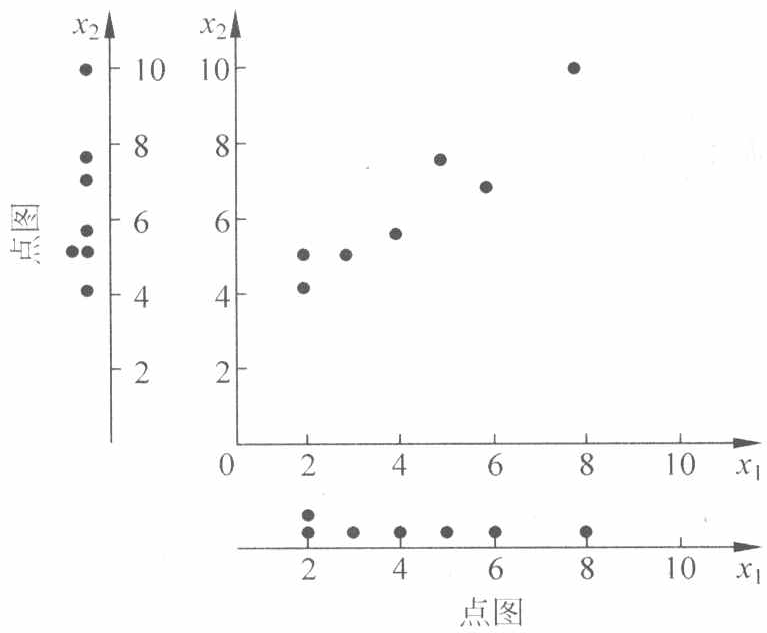
\includegraphics[width=64.9mm]{figs/fig_pg021_1.png}
\phantomsection\label{fig:1.1}\mvcap{图 1.1\quad 散布图和边缘点图}
\end{mvfigure}

\begin{mvfigure}
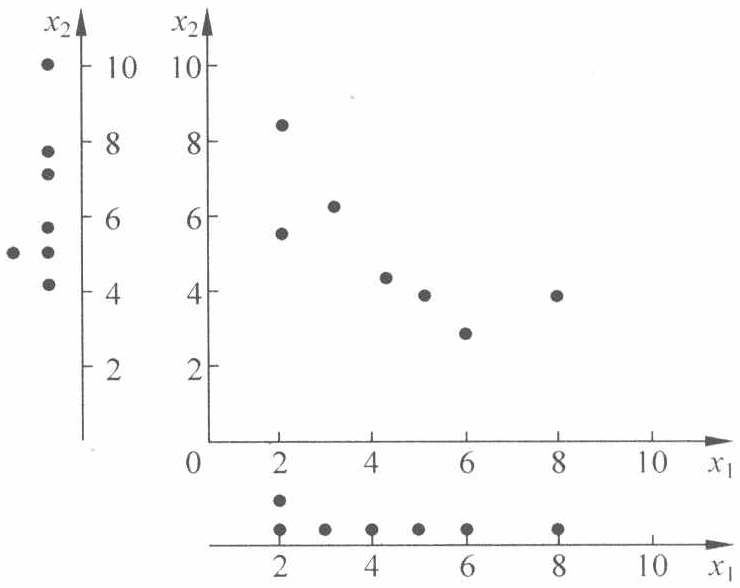
\includegraphics[width=62.7mm]{figs/fig_pg021_2.png}
\phantomsection\label{fig:1.2}\mvcap{图 1.2\quad 数据重新排列后的散布图和点图}
\end{mvfigure}

\hyperref[fig:1.1]{图 1.1} 和\hyperref[fig:1.2]{图 1.2} 中数据的不同取向无法通过单独的边缘点图辨别.然而,在两种情况下边缘点图是相同的,这个事实也无法立即从散布图中显示出来.这两种图解法不是对立的,而是相互补充的.

接下来两个例子可进一步说明通过图形表示可以传递的信息.

\mvbold{例 1.3}\quad (异常的观测值对样本相关系数的影响)

\begin{mvfigure}
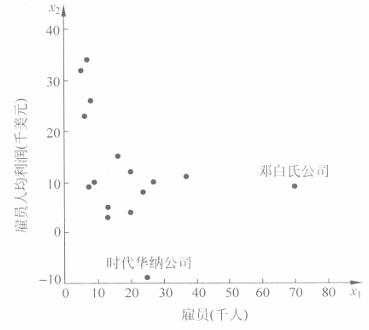
\includegraphics[width=72.9mm]{figs/fig_pg021_fig13.png}
\phantomsection\label{fig:1.3}\mvcap{图 1.3\quad 16 家出版公司的雇员人均利润和雇员人数}
\end{mvfigure}

% ---- 以下内容在源 PDF 中已损坏丢失（书页 9 图像自页高约 68\% 处截断）----
% 已依据用户提供的同一扫描件完好副本（clipboard-2026-10-04）补齐：
%   1) 正文一段："接下来两个例子可进一步说明通过图形表示可以传递的信息." + 例 1.3 标题
%   2) \hyperref[fig:1.3]{图 1.3}（纵轴"利润(千美元)"、刻度 20/30/40；数据点旁标注"邓白氏公司"）
% 来源：用户提供的同一扫描件完好副本（原书书页 9 对应页）
% UNCERTAIN: \hyperref[fig:1.3]{图 1.3} 的图题（caption）与下文在损坏区域中，未见；待用户补充后核对。

%% ===== pg-022 =====

% ---- pg-022 （书页 10） ----

的公司,但从每个雇员所创利润看是很“典型的”.时代华纳公司在雇员人数方面是很“典型的”,而在人均创利润上则相当的少(负值).

由 $x_1$ 和 $x_2$ 的值算出的样本相关系数是

\[
r_{12} = \begin{cases}
-0.39 & \text{对所有 16 个公司}\\
-0.56 & \text{对除邓白氏公司之外的所有公司}\\
-0.39 & \text{对除时代华纳公司之外的所有公司}\\
-0.50 & \text{对除邓白氏公司和时代华纳公司}\\
      & \text{之外的所有公司}
\end{cases}
\]

显然异常的观测值对于样本相关系数有着相当大的影响.\hfill$\blacksquare$

\mvbold{例 1.4}\quad（棒球数据的散布图）

1978 年 7 月 17 日,《体育画报》上一篇关于体育界工资的文章,为 $x_1 = $ 美国东部联盟棒球队为球员发放的工资总额提供了一些数据.

我们增加了 $x_2 = $ 1977 年的胜负比的数据.数据由\hyperref[tab:1.1]{表 1.1} 给出.

\begin{mvtable}
\begin{tabular}{lcc}
\toprule
队 & $x_1 = $ 运动员工资 & $x_2 = $ 胜负比 \\
\midrule
Philadelphia Phillies & 3 497 900 & 0.623 \\
Pittsburgh Pirates & 2 485 475 & 0.593 \\
St. Louis Cardinals & 1 782 875 & 0.512 \\
Chicago Cubs & 1 725 450 & 0.500 \\
Montreal Expos & 1 645 575 & 0.463 \\
New York Mets & 1 469 800 & 0.395 \\
\bottomrule
\end{tabular}
\phantomsection\label{tab:1.1}\mvtabcap{表 1.1\quad 关于美国东部联盟棒球队 1977 年工资和胜负比}
\end{mvtable}

\hyperref[fig:1.4]{图 1.4} 的散布图支持了一种看法: 冠军是可以买来的.当然,这种因果关系是无法证实的,因为实验不包括随机的工资总额的分配.因此,统计量无法回答这个问题: 如果 Mets 队有 400 万美元来支付运动员的薪水,是否就会赢?

\begin{mvfigure}
% 纵横比按原书实测校正：x 轴 167.6 px/单位、y 轴 417.5 px/单位
% （取 x=1.45cm/单位 → y = 1.45×417.5/167.6 = 3.61cm/单位；旧值 3.9cm 比原图高约 8%）
\begin{tikzpicture}[x=1.45cm,y=3.61cm,>=stealth]
\draw[->] (0,0) -- (4.6,0) node[below right=-1pt] {$x_1$};
\draw[->] (0,0) -- (0,1.03) node[above] {$x_2$};
\node[below,inner sep=1.5pt,font=\small] at (0,-0.018) {0};
\foreach \t in {1,2,3,4}{
  \draw (\t,0) -- (\t,-0.018);
  \node[below,inner sep=1.5pt,font=\small] at (\t,-0.018) {\t.0};
}
\foreach \t/\l in {0.4/0.400,0.8/0.800}{
  \draw (0,\t) -- (-0.10,\t);
  \node[left,inner sep=1.5pt,font=\small] at (-0.10,\t) {\l};
}
\foreach \x/\y in {1.4698/0.395,1.6456/0.463,1.7255/0.500,1.7829/0.512,2.4855/0.593,3.4979/0.623}{
  \fill (\x,\y) circle (1.5pt);
}
\node[below,font=\small] at (2.3,-0.13) {运动员工资(百万美元)};
\node[rotate=90,font=\small] at (-0.82,0.4) {胜负比};
\end{tikzpicture}
\phantomsection\label{fig:1.4}\mvcap{图 1.4\quad 从表 1.1 得到的工资和胜负比}
\end{mvfigure}

为了构造散布图,例如\hyperref[fig:1.4]{图 1.4},我们把\hyperref[tab:1.1]{表 1.1} 中的 6 对观测值看做是二维空间中 6 个点的坐标.此图让我们直观地检查相对于工资总额和胜负比的分组方法.\hfill$\blacksquare$

\mvbold{例 1.5}\quad（关于纸张强度观测结果的多重散布图）

纸是由几英尺宽的连续薄片制成的.由于纸中纤维的方向性,沿着机器造纸的方向测量的纸的强度,不同于沿着与机器造纸方向交叉或成直角的方向测量的结果.\hyperref[tab:1.2]{表 1.2} 列出了下%

%% ===== pg-023 =====

% ---- pg-023 （书页 11） ----

列变量的测量值.

\begin{mvtable}
\begin{longtable}{cccc}\toprule
\multirow{2}{*}{标本} & \multirow{2}{*}{密度} & \multicolumn{2}{c}{强度} \\
 & & 机器方向 & 交叉方向 \\
\midrule
\endfirsthead
\multicolumn{4}{c}{\zihao{6}续表}\\
\toprule
\multirow{2}{*}{标本} & \multirow{2}{*}{密度} & \multicolumn{2}{c}{强度} \\
 & & 机器方向 & 交叉方向 \\
\midrule
\endhead
\bottomrule
\endlastfoot

1 & 0.801 & 121.41 & 70.42 \\
2 & 0.824 & 127.70 & 72.47 \\
3 & 0.841 & 129.20 & 78.20 \\
4 & 0.816 & 131.80 & 74.89 \\
5 & 0.840 & 135.10 & 71.21 \\
6 & 0.842 & 131.50 & 78.39 \\
7 & 0.820 & 126.70 & 69.02 \\
8 & 0.802 & 115.10 & 73.10 \\
9 & 0.828 & 130.80 & 79.28 \\
10 & 0.819 & 124.60 & 76.48 \\
11 & 0.826 & 118.31 & 70.25 \\
12 & 0.802 & 114.20 & 72.88 \\
13 & 0.810 & 120.30 & 68.23 \\
14 & 0.802 & 115.70 & 68.12 \\
15 & 0.832 & 117.51 & 71.62 \\
16 & 0.796 & 109.81 & 53.10 \\
17 & 0.759 & 109.10 & 50.85 \\
18 & 0.770 & 115.10 & 51.68 \\
19 & 0.759 & 118.31 & 50.60 \\
20 & 0.772 & 112.60 & 53.51 \\
21 & 0.806 & 116.20 & 56.53 \\
22 & 0.803 & 118.00 & 70.70 \\
23 & 0.845 & 131.00 & 74.35 \\
24 & 0.822 & 125.70 & 68.29 \\
25 & 0.971 & 126.10 & 72.10 \\
26 & 0.816 & 125.80 & 70.64 \\
27 & 0.836 & 125.50 & 76.33 \\
28 & 0.815 & 127.80 & 76.75 \\
29 & 0.822 & 130.50 & 80.33 \\
30 & 0.822 & 127.90 & 75.68 \\
31 & 0.843 & 123.90 & 78.54 \\
32 & 0.824 & 124.10 & 71.91 \\
33 & 0.788 & 120.80 & 68.22 \\
34 & 0.782 & 107.40 & 54.42 \\
35 & 0.795 & 120.70 & 70.41 \\
36 & 0.805 & 121.91 & 73.68 \\
37 & 0.836 & 122.31 & 74.93 \\
38 & 0.788 & 110.60 & 53.52 \\
39 & 0.772 & 103.51 & 48.93 \\
40 & 0.776 & 110.71 & 53.67 \\
41 & 0.758 & 113.80 & 52.42 \\
\end{longtable}
\phantomsection\label{tab:1.2}\mvtabcap{表 1.2\quad 纸张性能测量结果}
\end{mvtable}

{\zihao{6} 资料来源：数据经 SONOCO 制造公司许可使用.}

%% ===== pg-024 =====

% ---- pg-024 （书页 12） ----

\[
\begin{aligned}
x_1 &= \text{密度(克 / 立方厘米)}\\
x_2 &= \text{强度(磅): 沿机器方向}\\
x_3 &= \text{强度(磅): 沿交叉方向}
\end{aligned}
\]

一种新颖的图形用来表示这些数据,见\hyperref[fig:1.5]{图 1.5}.散布图作为协方差阵列的非对角线元素,而盒形图作为对角线元素.用这一方法后者有不同的标度,故我们只用总的形状对称性给出信息,并为每个单独的特性提供可能的离群值.可对图形和异常的观测值来观察散布图.在\hyperref[fig:1.5]{图 1.5} 中,有一个异常的观测值: 样本 25 的密度.某些散布图表明,其观测值是相互分离的两簇.阵列的这些散布图将在下一节中新的软件图解方法的讨论中还会涉及.

\begin{mvfigure}
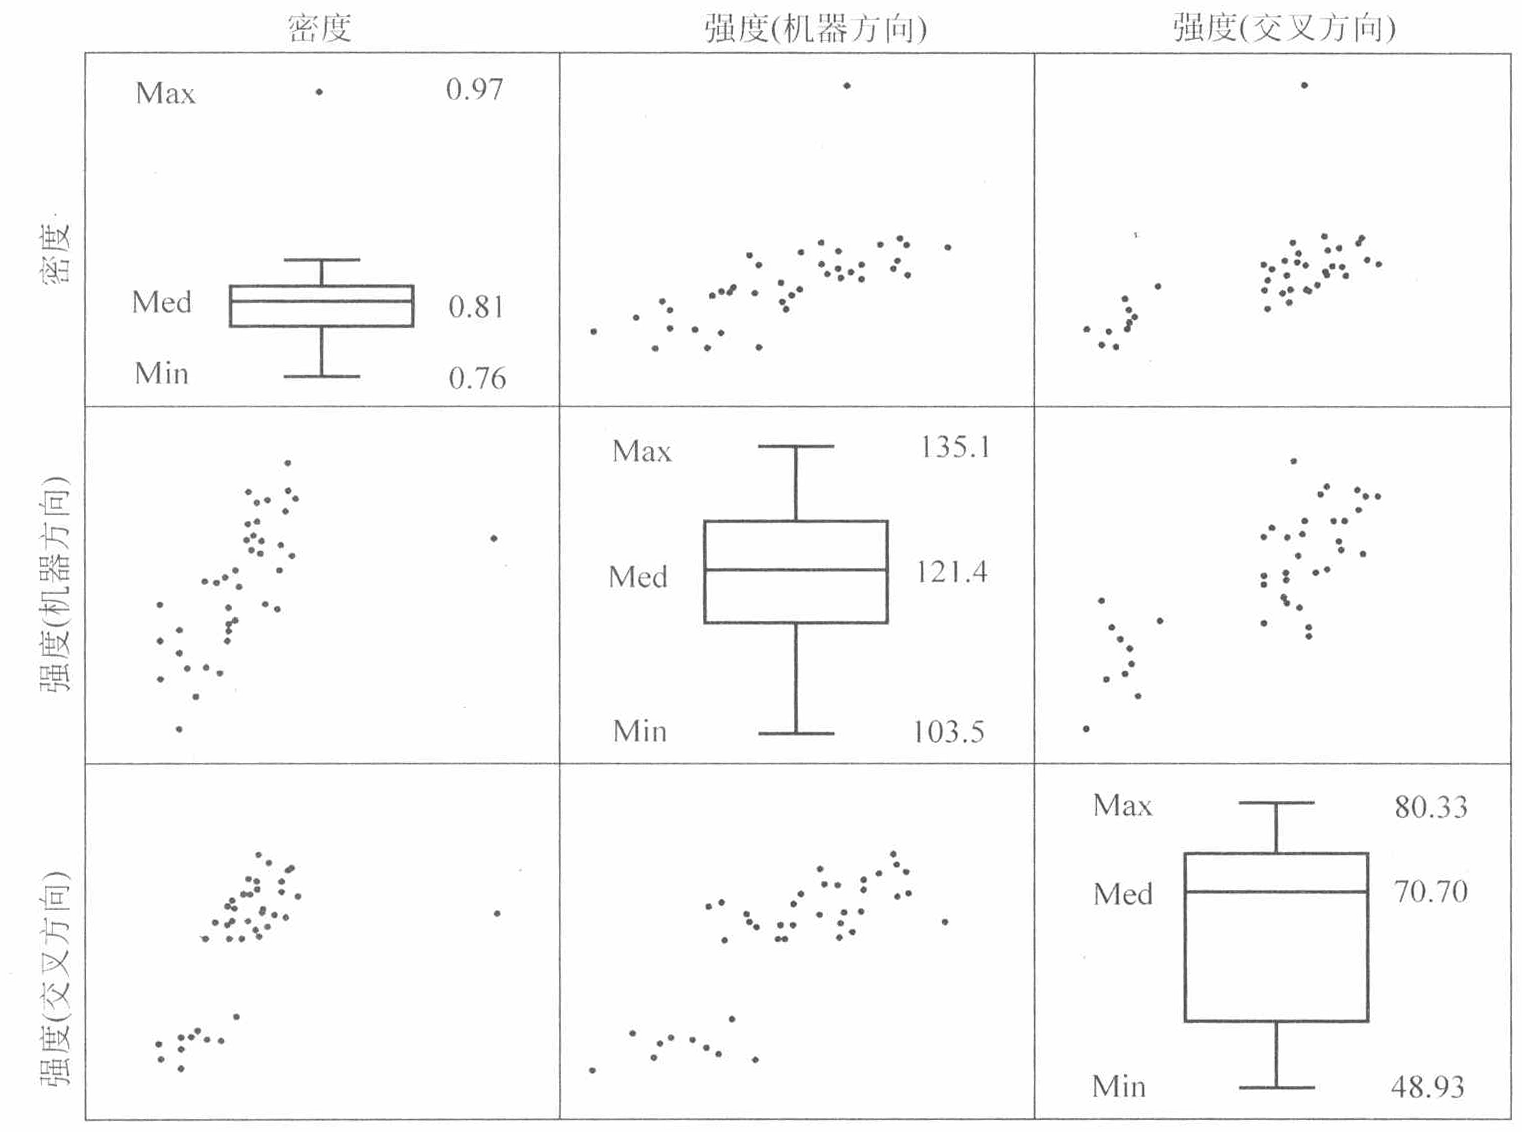
\includegraphics[width=128.9mm]{figs/fig_pg024_1.png}
\phantomsection\label{fig:1.5}\mvcap{图 1.5\quad 来自表 1.2 的纸张性能数据的散布图和盒形图}
\end{mvfigure}

在一般的多种响应的情况下, $p$ 个变量同时进行 $n$ 项记录.应该为几对重要的变量作散布图,并且如果工作量没有大到得不偿失,应该对每一对变量作图.

由于我们被限定在一个三维世界,我们经常无法描述整个的数据集合.然而,两种进一步的数据几何表示为观察多元统计方法提供了一个重要的概念框架.假如在三维空间捕捉到数据的本质是可能的,就可以用实际图形表示.

\mvbold{$p$ 维空间中的 $n$ 个点($p$ 维散布图)}\quad 考虑将散布图自然地扩展到 $p$ 维空间,其中 $p$ 个观测结果

\[
(x_{j1}, x_{j2}, \cdots, x_{jp})
\]

表示一个点在 $p$ 维空间中的坐标在第 $j$ 项的值.每个坐标轴与变量相对应,则第 $j$ 个点沿着第一个坐标轴是 $x_{j1}$ 个单位,沿第二个坐标轴是 $x_{j2}$ 个单位,$\cdots$,沿第 $p$ 个坐标轴是 $x_{jp}$ 个单位的点.由此得到的有 $n$ 个点的结果的图形不仅显示了变异性的总的模型,而且会显示出 $n$ 项中

%% ===== pg-025 =====

% ---- pg-025 （书页 13） ----

的相似(和不同)之处.项目的分组会在这个表象中表现出来.

下面的例子说明三维散布图.

\mvbold{例 1.6}\quad （寻找降维结构）

一位动物学家得到了 $n=25$ 组蜥蜴的数据.其重量(体重)的单位为克,嘴到排泄口的体长(SVL)和后肢跨距(HLS)的单位为毫米.\hyperref[tab:1.3]{表 1.3} 中列出了对应的数据.

\begin{mvtable}
\begin{tabular}{cccc|cccc}
\toprule
蜥蜴 & 体重 & SVL & HLS & 蜥蜴 & 体重 & SVL & HLS \\
\midrule
1 & 5.526 & 59.0 & 113.5 & 14 & 10.067 & 73.0 & 136.5 \\
2 & 10.401 & 75.0 & 142.0 & 15 & 10.091 & 73.0 & 135.5 \\
3 & 9.213 & 69.0 & 124.0 & 16 & 10.888 & 77.0 & 139.0 \\
4 & 8.953 & 67.5 & 125.0 & 17 & 7.610 & 61.5 & 118.0 \\
5 & 7.063 & 62.0 & 129.5 & 18 & 7.733 & 66.5 & 133.5 \\
6 & 6.610 & 62.0 & 123.0 & 19 & 12.015 & 79.5 & 150.0 \\
7 & 11.273 & 74.0 & 140.0 & 20 & 10.049 & 74.0 & 137.0 \\
8 & 2.447 & 47.0 & 97.0 & 21 & 5.149 & 59.5 & 116.0 \\
9 & 15.493 & 86.5 & 162.0 & 22 & 9.158 & 68.0 & 123.0 \\
10 & 9.004 & 69.0 & 126.5 & 23 & 12.132 & 75.0 & 141.0 \\
11 & 8.199 & 70.5 & 136.0 & 24 & 6.978 & 66.5 & 117.0 \\
12 & 6.601 & 64.5 & 116.0 & 25 & 6.890 & 63.0 & 117.0 \\
13 & 7.622 & 67.5 & 135.0 & & & & \\
\bottomrule
\end{tabular}
\phantomsection\label{tab:1.3}\mvtabcap{表 1.3\quad 蜥蜴数据}
\end{mvtable}

{\zihao{6} 资料来源：数据经 Kevin E. Bonine 许可使用.}

尽管有 3 种大小的测量数据,我们感兴趣的是大部分的变化是否都基本限制在二维甚至于一维空间上.

为了回答上面关于降维的问题,在\hyperref[fig:1.6]{图 1.6} 中我们画出了数据的三维散布图.很明显大部分的变化都集中在一条一维的直线上.知道了沿这些点的主轴直线的位置,也就大致知道了这三维数据(重量,SVL 和 HLS)的情况.

可是,如果在一个变量的变化比其他的变化大得多的情况下,这种分析会误导大家.所以,我们首先要将数值标准化,即 $z_{jk} = (x_{jk} - \bar{x})/\sqrt{s_{kk}}$,这样各个变量在散布图中有相同的作用.\hyperref[fig:1.7]{图 1.7} 为标准化后变量的散布图,大部分的变化都能被由这些点决定的直线所对应的单个变量来解释.

\begin{mvfigure}
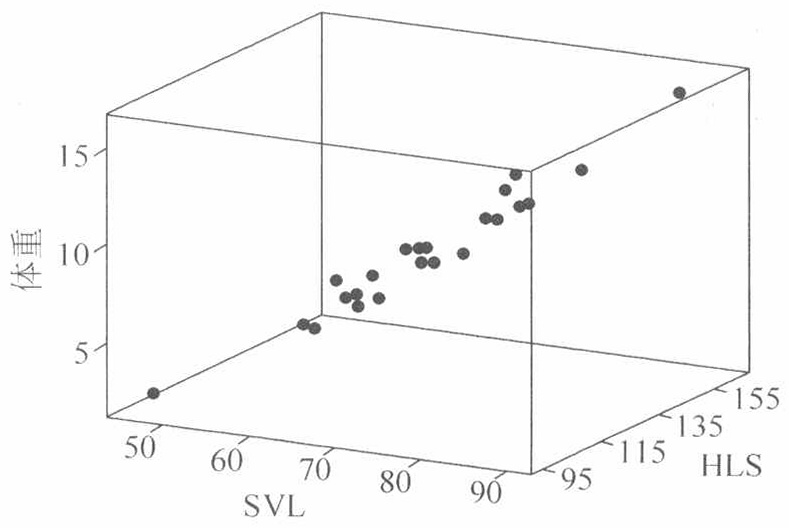
\includegraphics[width=66.8mm]{figs/fig_pg025_1.png}
\phantomsection\label{fig:1.6}\mvcap{图 1.6\quad 表 1.3 的蜥蜴数据的三维散布图}
\end{mvfigure}

\begin{mvfigure}
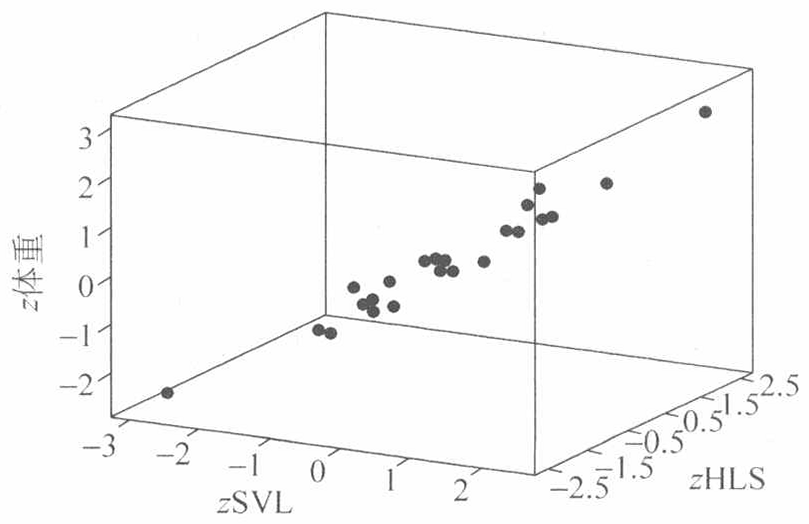
\includegraphics[width=68.4mm]{figs/fig_pg025_2.png}
\phantomsection\label{fig:1.7}\mvcap{图 1.7\quad 标准化后数据的三维散布图\quad$\blacksquare$}
\end{mvfigure}

% UNCERTAIN: pg-025 \hyperref[fig:1.7]{图 1.7} 图题行右端实心方块 ■ 为原书"节/例结束"符号，已用 $\blacksquare$ 还原（参 pg-017 先例）。

%% ===== pg-026 =====

% ---- pg-026 （书页 14） ----
一个三维散布图通常能用来揭示群组结构.

\mvbold{例 1.7} （三维情形下群组结构的搜寻）

参见例 1.6, 考虑雄性蜥蜴和雌性蜥蜴在三维数据空间中是否占据空间的不同部分, 是很有趣的. \hyperref[tab:1.3]{表 1.3} 中对应的数据中, 蜥蜴的性别(用行表示)分别为

\[
\begin{array}{cccccccccccc}
f & m & f & f & m & f & m & f & m & f & m & m \\
m & m & m & f & m & m & m & f & f & m & f & f
\end{array}
\]

\hyperref[fig:1.8]{图 1.8} 重复了原来的数据散布图, 只不过这里用空心点表示雌性, 用实心点表示雄性. 显然, 雄性的体型一般都比雌性的要大.

\begin{mvfigure}
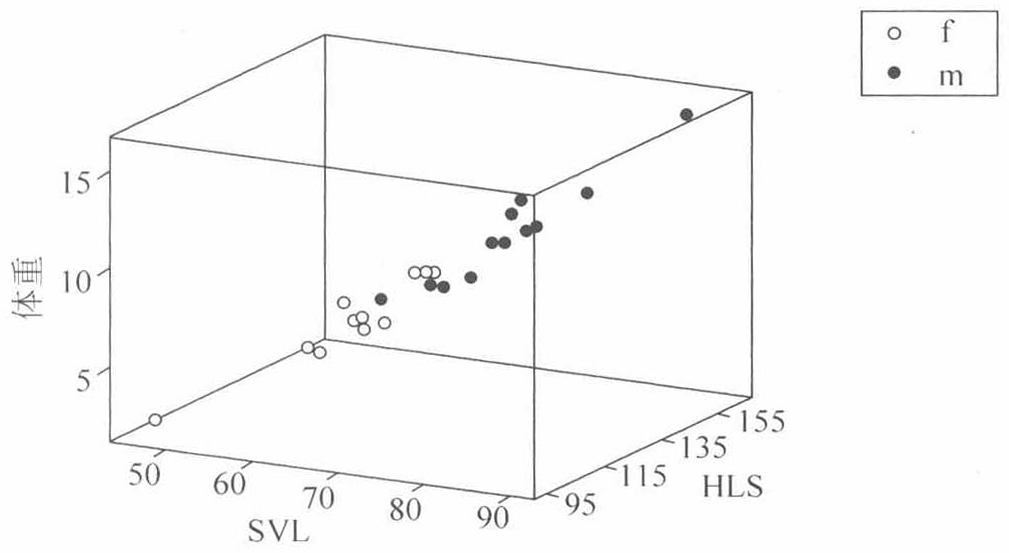
\includegraphics[width=85.3mm]{figs/fig_pg026_1.png}
\phantomsection\label{fig:1.8}\mvcap{图 1.8\quad 雄性和雌性蜥蜴的三维散布图}
\end{mvfigure}

$n$ 维空间中 $p$ 个点 \quad $p$ 个变量的 $n$ 个观测结果也可看做是 $n$ 维空间中的 $p$ 个点. $\bm{X}$ 的每一列确定其中的一个点. 由第 $i$ 个变量的所有 $n$ 个观测值组成的第 $i$ 列确定了第 $i$ 个点

\[
\begin{bmatrix}
x_{1i} \\
x_{2i} \\
\vdots \\
x_{ni}
\end{bmatrix}
\]

在第 3 章中, 我们将介绍 $n$ 维空间中点的封闭性如何与相关变量之间联合的测量相联系.

\section{数据的展示及图表示}  % 原书 1.4
\phantomsection\label{sec:1.4}

强大的个人电脑与计算机工作站的迅速发展, 导致为数据分析和图解法而设计的复杂统计软件增加. 例如, 坐在书桌前就能通过灵巧的计算机生成的图片来观察多维数据的本质, 这已是可能的. 这些图片对于了解数据极有帮助, 并常常防止许多错误的出现以及随后的推理上的问题.

正如我们将在第 8 章和第 12 章看到的, 有许多方法企图用不多的维数表示 $p$ 维观测值, 使得每对观测值的初始距离(或相似性)几乎保持不变. 一般的, 如果多维观测值可以表现在二维空间中, 则离群值, 各种关系及可分辨的分组常常可以用眼睛辨别. 我们将讨论并说明几种在二维空间中显示多元数据的方法. 关于图解法的更多讨论的优秀初始资料见文献[11].

%% ===== pg-027 =====

% ---- pg-027 （书页 15） ----

\mvsub{多种二维散布图的联系}

在许多令人兴奋的新的图解法中,有一种是用计算机来联系众多二维散布图.

\mvbold{例 1.8}\quad（散布图的联系及刷亮）

参看\hyperref[tab:1.2]{表 1.2} 的纸张性能数据,我们来说明二维散布图的联系.这些数据表示了三个变量的测量值: $x_1=$ 密度, $x_2=$ 沿机器方向的强度; $x_3=$ 与机器交叉方向的强度.\hyperref[fig:1.9]{图 1.9} 显示了一个 $3\times3$ 阵列,由每对变量做成的二维散布图组成.例如,图中左上角那个图是由 $(x_1, x_2)$ 这一对观测值做成的散布图.即, $x_1$ 的值是沿着水平坐标轴绘图,而 $x_2$ 的值则沿着垂直坐标轴绘图.图中右下角的散布图是由 $(x_2, x_3)$ 这对观测值做成的,将坐标轴颠倒一下就成.图中其他散布图的相应说明也成立.注意变量及它们的二维排列在框图中表示时是沿着西南-东北对角线方向的.将\hyperref[fig:1.9]{图 1.9} 的 $(x_1, x_2)$ 散布图中明显的离群值做出标记(选择出),产生了\hyperref[fig:1.10]{图 1.10}(a),离群值被标为样本 25,同一个数据点在所有的散布图中被突出标示.可发现样本 25 也以离群值出现在 $(x_1, x_3)$ 的散布图中,但不是 $(x_2, x_3)$ 的散布图的离群值.删掉这个样本形成改变后的见\hyperref[fig:1.10]{图 1.10}(b)散布图.

\begin{mvfigure}
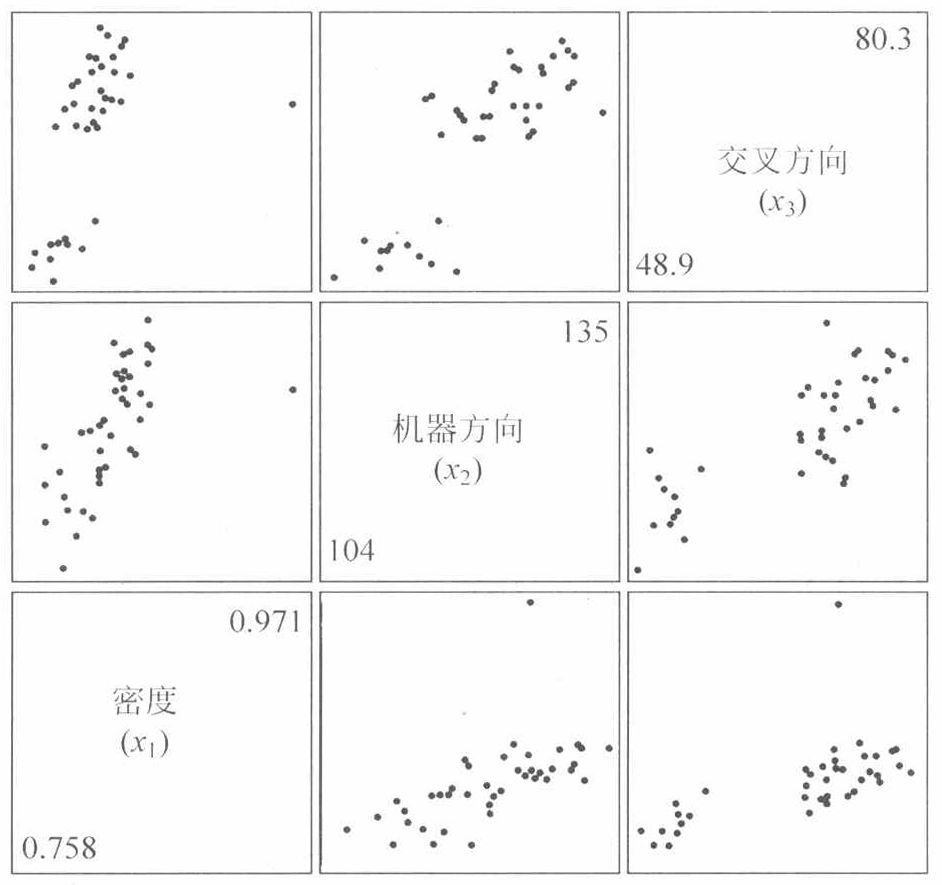
\includegraphics[width=79.8mm]{figs/fig_pg027_1.png}
\phantomsection\label{fig:1.9}\mvcap{图 1.9\quad 表 1.2 纸张性能数据散布图}
\end{mvfigure}

从\hyperref[fig:1.10]{图 1.10} 中,我们注意到,在 $(x_3, x_c)$ 散布图中一些点看起来与其他的点没有联系.用一个虚线矩形框将这些点框起,在其他所有散布图中高亮显示这些选中的点,如\hyperref[fig:1.11]{图 1.11}(a) 所示.进一步检查显示出样本 16$\sim$21,样本 34 及样本 38$\sim$41 实际上是从一卷旧纸中选取的样本,它们是为了使生产的卡纸板有足够的厚度.删除离群值及与旧纸相关的点,调整剩下的观测值的排列,得到\hyperref[fig:1.11]{图 1.11}(b)中的散布图.

高亮显示对应于一个变量散布图中被选中的区域的点,称为刷亮.刷亮可以从一个矩形开始,如\hyperref[fig:1.11]{图 1.11}(a),然后,刷子可以移动给出一个高亮显示点的序列.这个过程可在任何时候停止,以得到一个当前情况的瞬态.\quad$\blacksquare$

像例 1.8 中的那种散布图对数据分析非常有帮助.另一个新的重要的图解法使用了计算机软件,使数据分析者可用种种不同的三维透视图来观察高维数据.这可以动态地,持续地进%

%% ===== pg-028 =====

% ---- pg-028 （书页 16） ----

\begin{mvfigure}
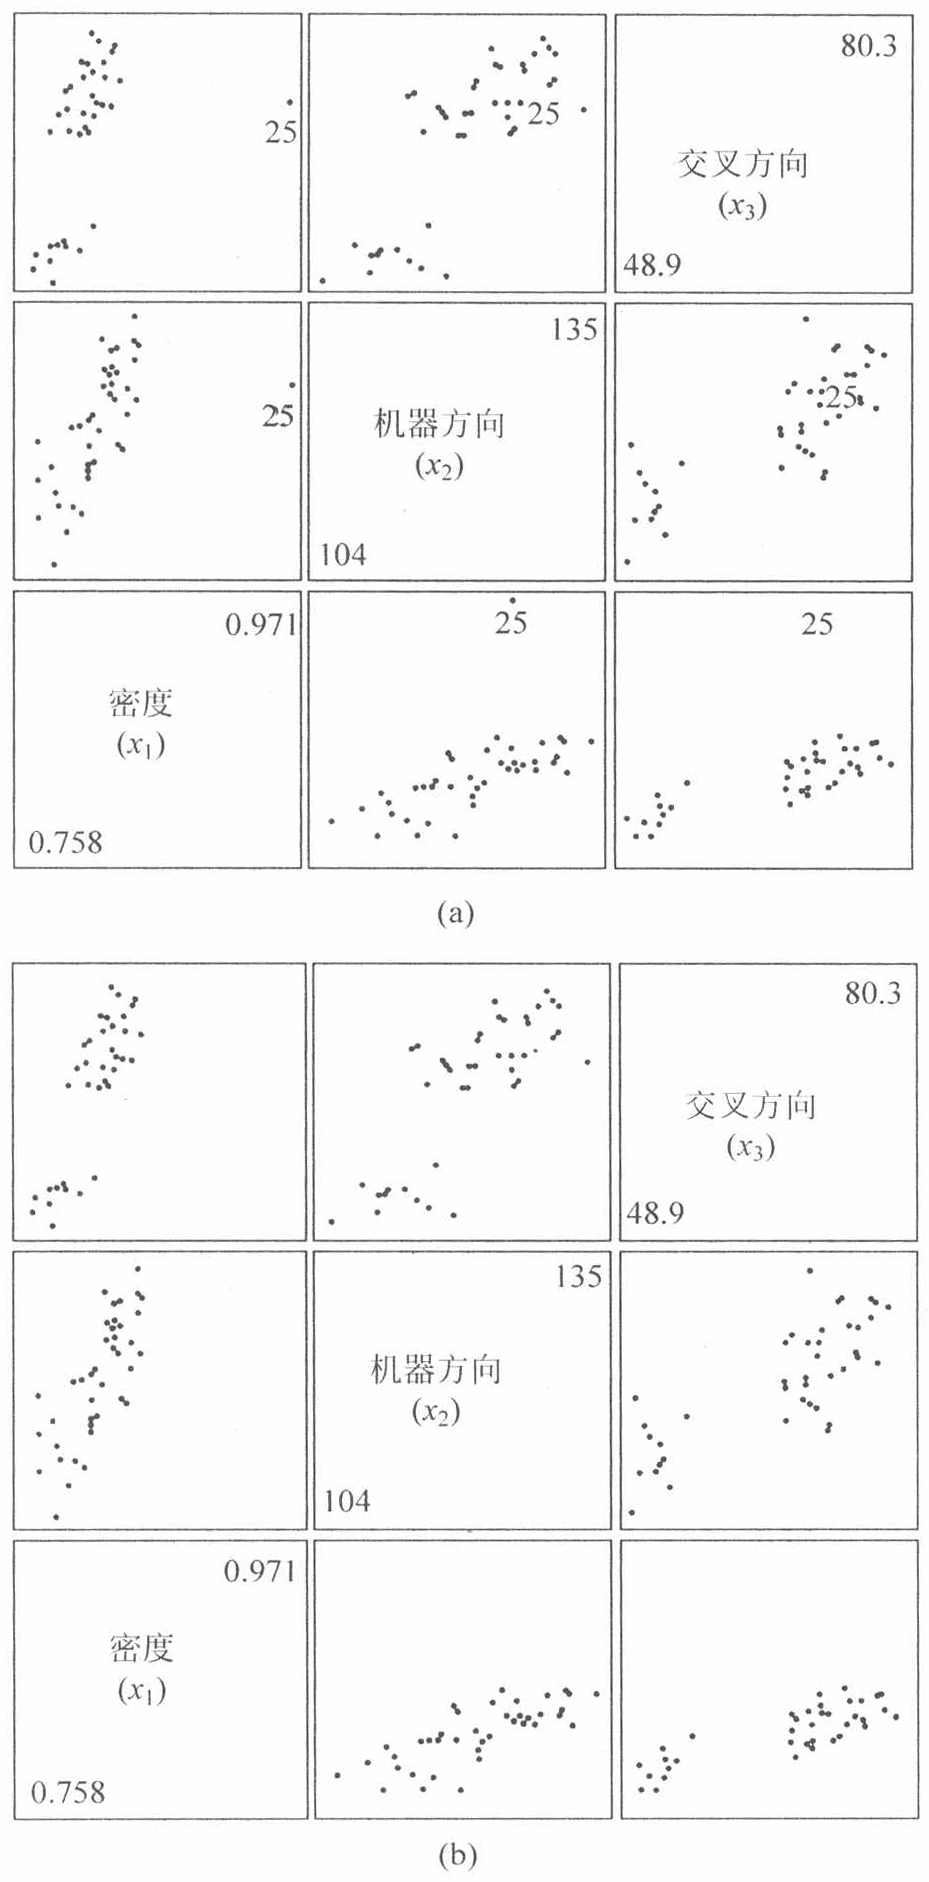
\includegraphics[width=78.7mm]{figs/fig_pg028_1.png}
\phantomsection\label{fig:1.10}\mvcap{图 1.10\quad 纸张性能数据的改进散布图}
{\zihao{6} (a) 选择离群值(25); (b) 删除离群值(25)}
\end{mvfigure}

行直到获得足够的信息.关于动态图解法的全面讨论可参见文献[1].关于与主机联在一起工作的多元探测图解分析的一个策略参见[32],该策略的动机是为了得到一个可寻找多元数据结构的常规程序.

\mvbold{例 1.9} (在三维空间作图)

第 4 章中的\hyperref[tab:4.3]{表 4.3} 给出了木材硬度的四个不同测量值.在例 4.14 中,样本(木板)16 及可能样本(木板)9 被标为异常观测值.\hyperref[fig:1.12]{图 1.12}(a),(b)和(c)显示出硬度数据在 $x_1,x_2,x_3$ 空间上%

%% ===== pg-029 =====

% ---- pg-029 （书页 17） ----

\begin{mvfigure}
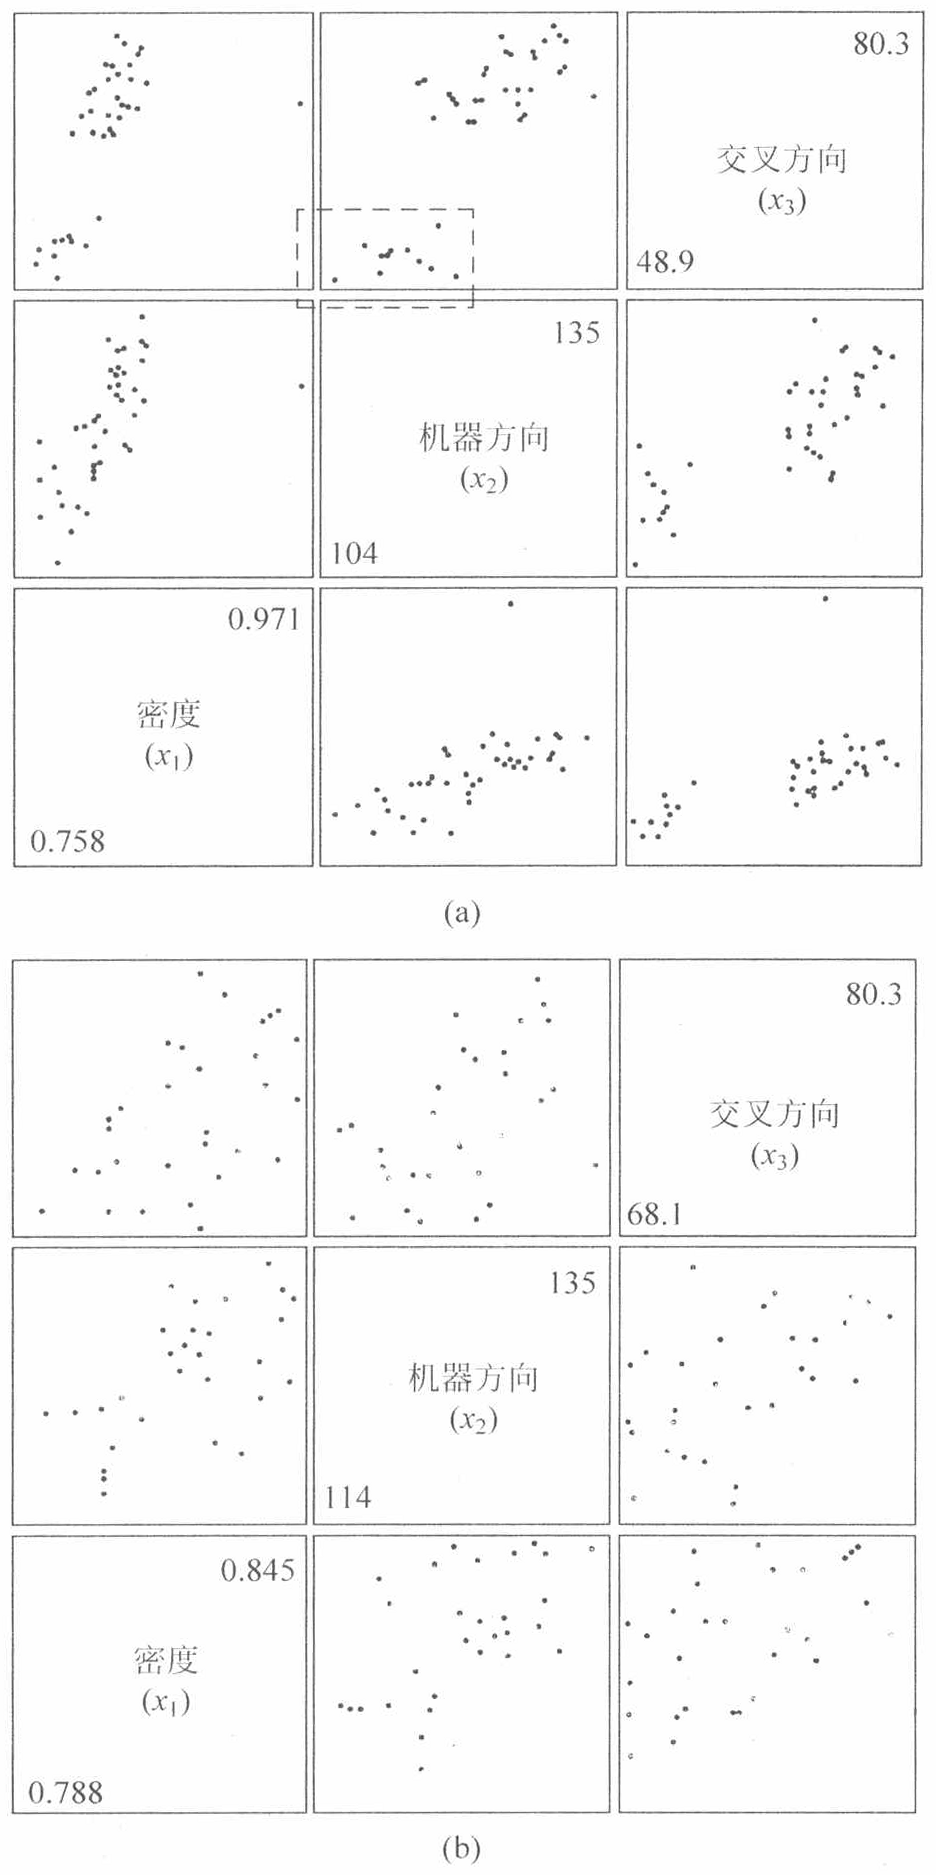
\includegraphics[width=79.2mm]{figs/fig_pg029_1.png}
\phantomsection\label{fig:1.11}\mvcap{图 1.11\quad 改进的散布图对(a)选择的点的组和(b)删去标本 25 在内的诸点,并重画散布图}
\end{mvfigure}

的透视图.这些视图是通过连续地旋转及转换三维坐标轴得到的.旋转坐标轴我们可得到对数据的三维外观的更好的了解.\hyperref[fig:1.12]{图 1.12}(d)给出硬度数据在 $x_3, x_1, x_2$ 空间的图片.注意到\hyperref[fig:1.12]{图 1.12}(a)和(d)清楚地证实了样本 9 和 16 是离群值.样本 9 的数值在所有的三维坐标中都非常大.把\hyperref[fig:1.12]{图 1.12}(a)的坐标轴逆时针旋转得到\hyperref[fig:1.12]{图 1.12}(b),两个异常的观测值在这个视图中被屏蔽了.进一步旋转坐标轴 $x_2, x_3$ 得到\hyperref[fig:1.12]{图 1.12}(c);此时离群值之一标本 16 隐藏起来.

通过这些缓慢旋转的数据进行目测有时可获得额外的认识.统计学家们对这种动态的方式刚刚才开始了解和利用.

%% ===== pg-030 =====

% ---- pg-030 （书页 18） ----

\begin{mvfigure}
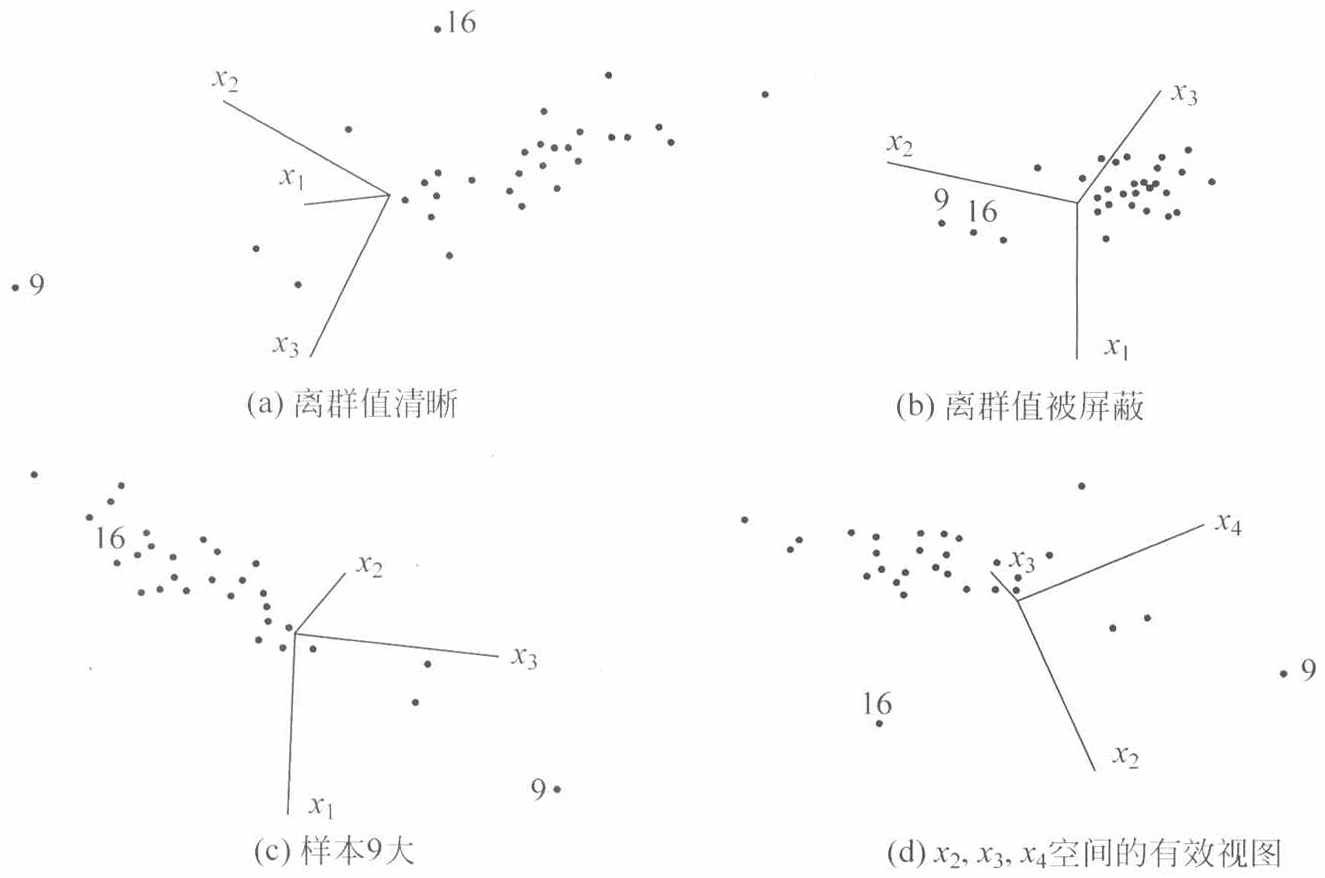
\includegraphics[width=112.2mm]{figs/fig_pg030_1.png}
\phantomsection\label{fig:1.12}\mvcap{图 1.12\quad 对木材硬度数据的三维透视}
\end{mvfigure}

像\hyperref[fig:1.12]{图 1.12} 这样的图使我们可以迅速地识别出那些与其他数据不一致的观测值和可能会严重影响到基于标准数据生成模型所得推论的观测值.

\mvsub{生长曲线图}

如果在每年生日的时候都测一下小孩的身高,然后将点画出来,连接成图.这就是一个典型的生长曲线图.一般来说,如果测量值随着时间有上升、下降或者既有上升又有下降的情况,我们就在相同的单位和对象下,可以重复测量该值,得到生长曲线图.

\mvbold{例 1.10} (生长曲线阵列)

阿拉斯加渔业和狩猎部门为了保持灰熊健康的种群量,对灰熊实施监测.熊被催眠针催眠然后挂在三脚架上测量它们的体重,并用钢卷尺测量它们的身长.\hyperref[tab:1.4]{表 1.4} 中给出了 7 只母熊在 2,3,4 和 5 岁时的体重(简记为 Wt,单位: 公斤)和身长(简记为 Lngth,单位: 厘米)的数据.

\begin{mvtable}
\begin{tabular}{ccccccccc}
\toprule
熊序号 & Wt2 & Wt3 & Wt4 & Wt5 & Lngth2 & Lngth3 & Lngth4 & Lngth5 \\
\midrule
1 & 48 & 59 & 95 & 82 & 141 & 157 & 168 & 183 \\
2 & 59 & 68 & 102 & 102 & 140 & 168 & 174 & 170 \\
3 & 61 & 77 & 93 & 107 & 145 & 162 & 172 & 177 \\
4 & 54 & 43 & 104 & 104 & 146 & 159 & 176 & 171 \\
5 & 100 & 145 & 185 & 247 & 150 & 158 & 168 & 175 \\
6 & 68 & 82 & 95 & 118 & 142 & 140 & 178 & 189 \\
7 & 68 & 95 & 109 & 111 & 139 & 171 & 176 & 175 \\
\bottomrule
\end{tabular}
\phantomsection\label{tab:1.4}\mvtabcap{表 1.4\quad 母熊数据}
\end{mvtable}

{\zihao{6} 资料来源: 数据经 H. Roberts 许可使用.}

%% ===== pg-031 =====

% ---- pg-031 （书页 19） ----

首先,对每只熊,我们描出体重对年龄的图然后用直线连接,这样能够近似给出生长曲线图.\hyperref[fig:1.13]{图 1.13} 是所有 7 只熊的生长曲线图.很明显的是,第 5 只熊相对于其他来说有很大不同.这是外族还是自然变异的?在野外,熊的体重是用磅来度量的.进一步的观测表明,这种情况是由于助手在建立电子数据库时,没有将单位换算成公斤,正确的体重为$(45,66,84,112)$公斤.

\begin{mvfigure}
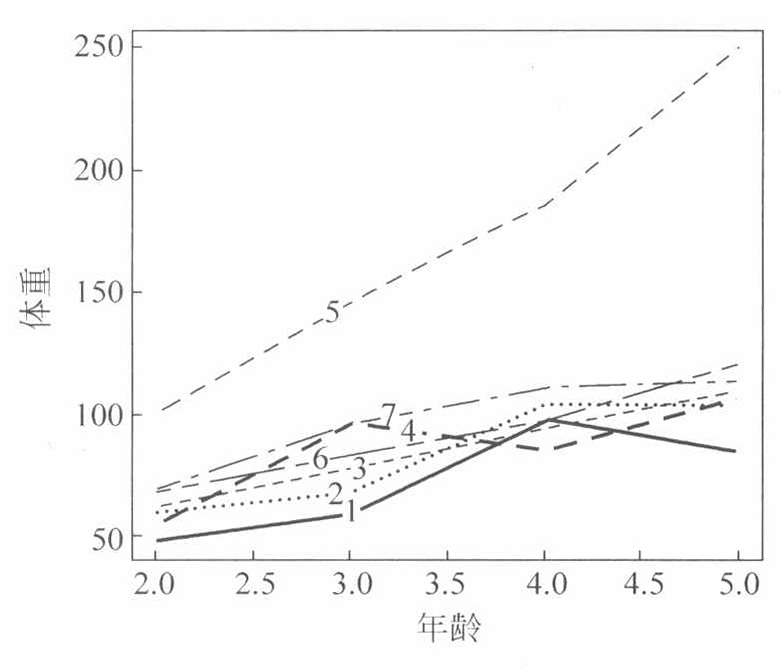
\includegraphics[width=66.2mm]{figs/fig_pg031_1.png}
\phantomsection\label{fig:1.13}\mvcap{图 1.13\quad 7 只母灰熊体重的联合生长曲线列}
\end{mvfigure}

因为在一个联合生长曲线图上观测个体变化很难,于是可以逐一画出一系列单个生长曲线,这样相似性和差别都能够很容易地观测出来.\hyperref[fig:1.14]{图 1.14} 给出了 7 条体重生长曲线,有些体重生长曲线是线性的,有些是二次的.

\begin{mvfigure}
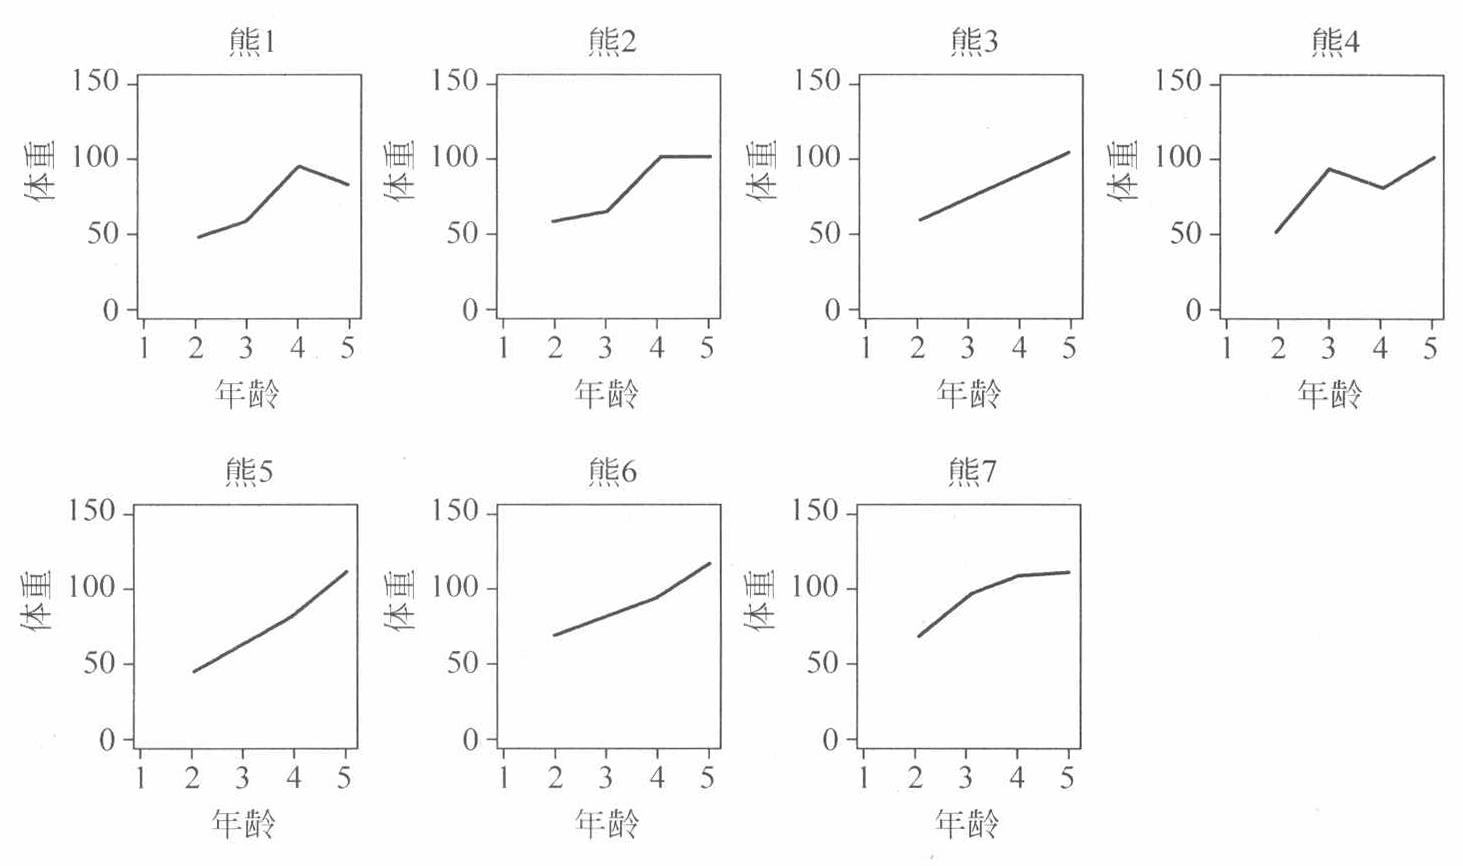
\includegraphics[width=123.8mm]{figs/fig_pg031_2.png}
\phantomsection\label{fig:1.14}\mvcap{图 1.14\quad 单个母灰熊体重的生长曲线列}
\end{mvfigure}

\hyperref[fig:1.15]{图 1.15} 给出了单个母灰熊身长的生长曲线列.有一只熊好像在第 2 年到第 3 年变得越来越短了,但是研究人员知道,测量身长用的卷尺会由于打了镇静剂的熊的姿势脱落,进而导致结果的偏差.

现在我们转向多元数据在二维空间中的两个常见的图示表示法: 星形和切尔诺夫脸.

%% ===== pg-032 =====

% ---- pg-032 （书页 20） ----

\begin{mvfigure}
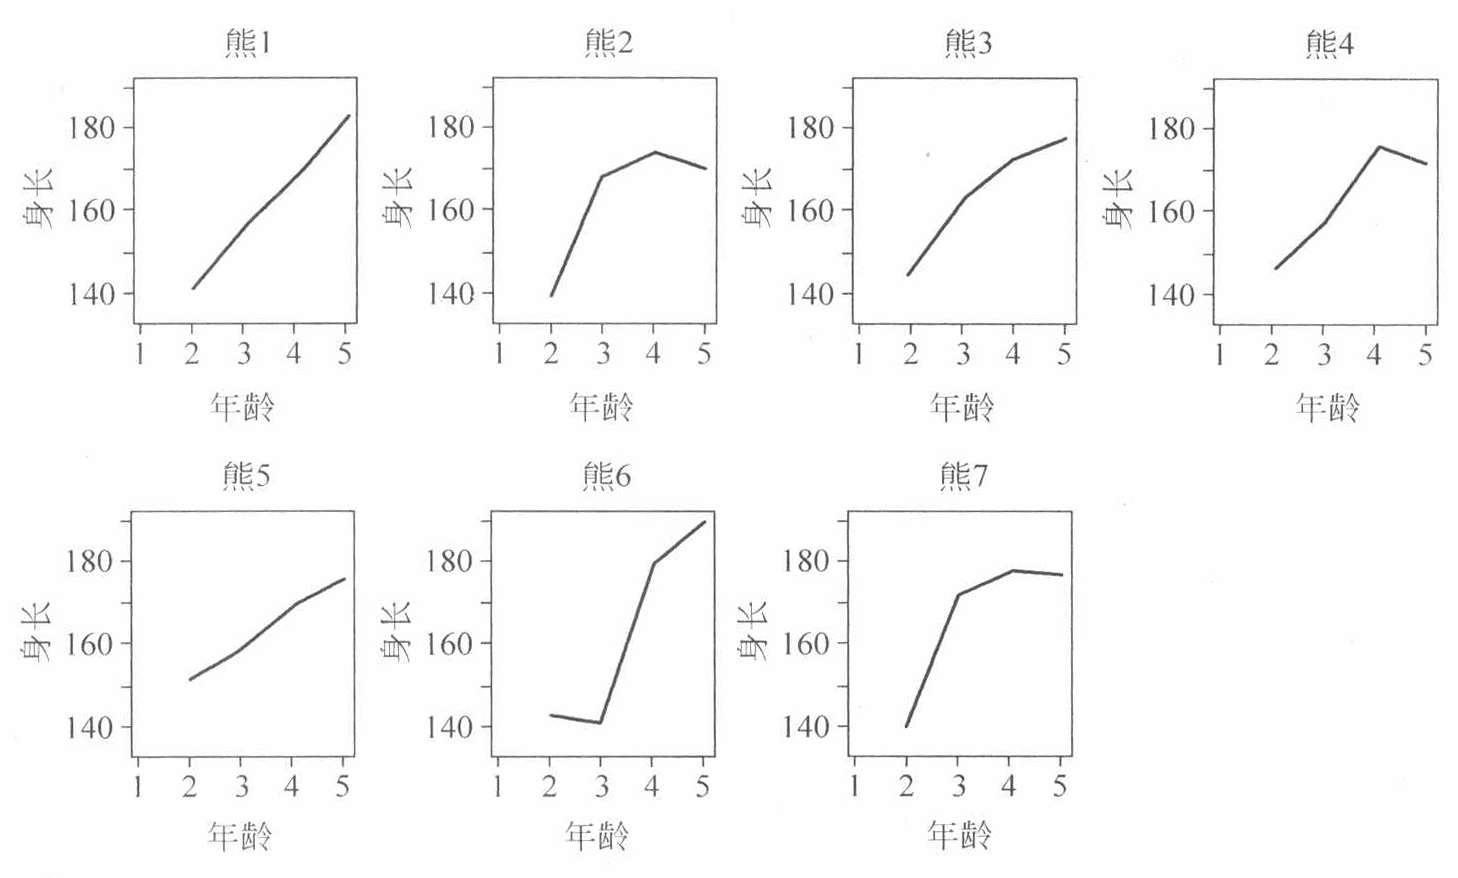
\includegraphics[width=123.5mm]{figs/fig_pg032_1.png}
\phantomsection\label{fig:1.15}\mvcap{图 1.15\quad 单个母灰熊身长的生长曲线列}
\end{mvfigure}

\mvsub{星形}

假设每个数据单元由 $p\geqslant 2$ 个变量的非负观测值组成.在二维空间中,我们可构造具有固定(参照)半径的圆,从圆心引出 $p$ 条等距的射线,这些射线的长度代表变量的数值,以直线连接射线的端点即形成一个星形.每个星形代表一个多元观测值,这些星形可根据它们(主观的)的相似性分组.

在构造星形时,将观测值标准化常常会有所帮助.在这种情况下,一些观测值会是负数.观测值可以重新表示,使得圆心代表整个数据集中的最小标准化观测值.

\mvbold{例 1.11}\quad(星形的实用数据)

\hyperref[fig:1.16]{图 1.16} 给出 5 个星形图.它们代表第 12 章\hyperref[tab:12.4]{表 12.4} 所列出的 22 个公用事业公司中的前 5 个公司的观测值.共有 8 个变量,因此,这些星形是变形的八边形.

所有变量的观测值都是经过标准化的.在这前 5 个公司中,对任何变量最小的标准化观测值是 $-1.6$.将这个值作为零点,沿着从圆心引出的 8 条等角射线以相同的比例画出 8 个变量,这些变量以 12 点钟的位置为起点,按顺时针方向排序.

初看起来,这些公司中没有一个与其他任何一个是相似的.由于星形的构造方法,不管怎样,每个变量在感观上权数是相等的.如果我们仔细观察变量 6(以每年使用千瓦时为单位的销售额总量)和变量 8(以美分/千瓦时为单位的燃料费用),则发现,波士顿爱迪生和联合爱迪生是相似的(小变量 6,大变量 8),以及亚利桑那公共服务公司、中央路易斯安那电力公司和联邦爱迪生公司是相似的(中等变量 6 和中等变量 8).

\mvsub{切尔诺夫脸}

人们的反应表现在脸上.切尔诺夫(见文献[4])假定用二维平面的脸来表示 $p$ 维观测结果,脸的特征(如脸的形状,嘴的弯曲率,鼻子的长度,眼睛的大小,瞳孔的位置等等)是由 $p$ 个变量的测量值所决定的.

按照最初的设计,切尔诺夫脸可处理多达 18 个变量.脸部容貌对应的变量的分配是由实%

%% ===== pg-033 =====

% ---- pg-033 （书页 21） ----

验者完成的,不同选择会产生不同的结果.为了取得令人满意的表示常常需要一些重复步骤.

\begin{mvfigure}
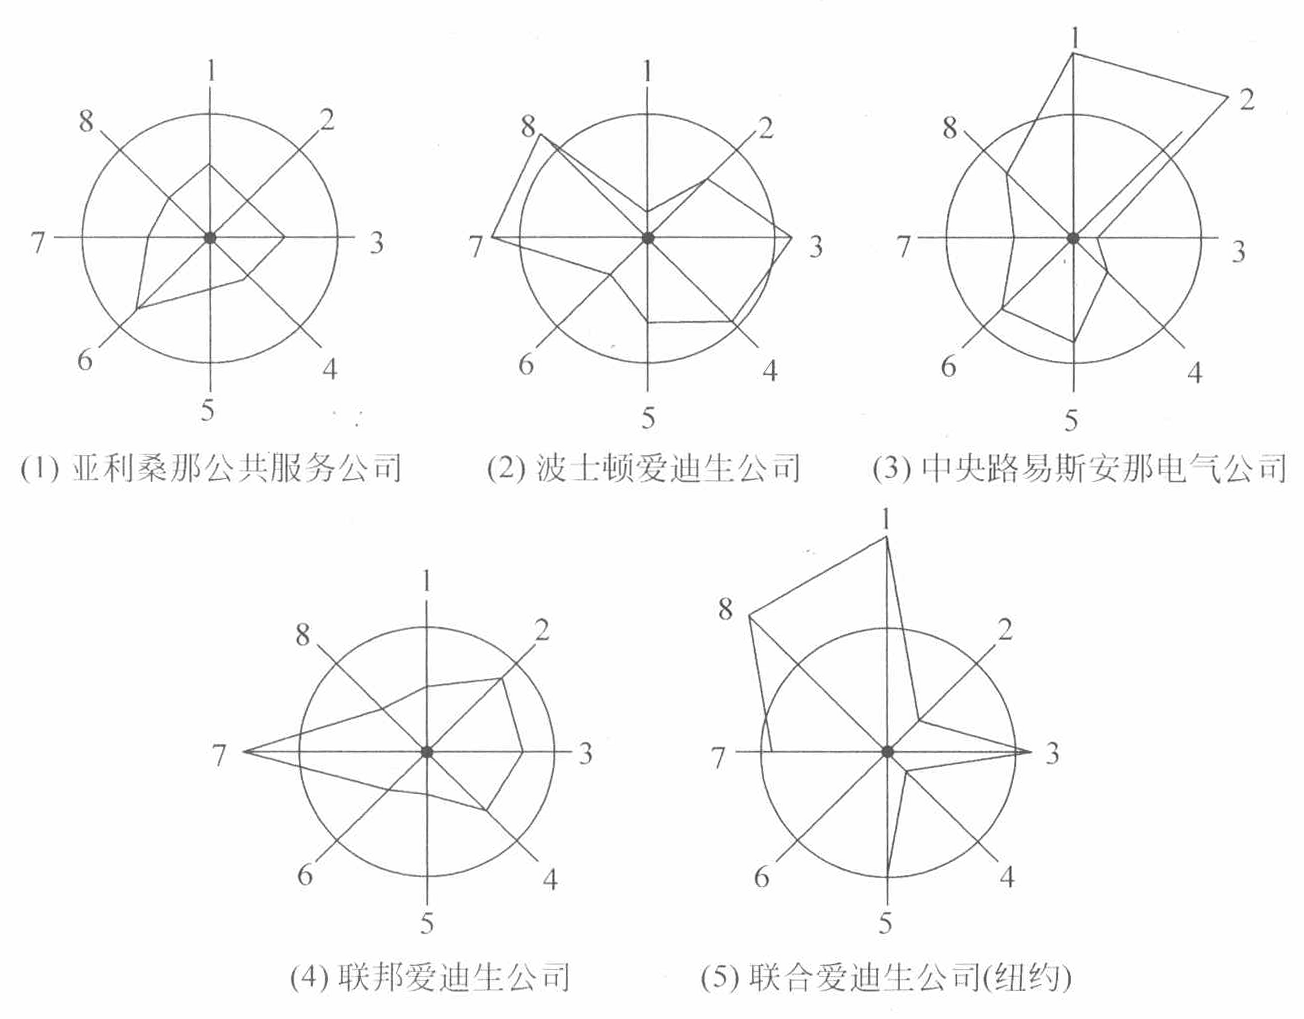
\includegraphics[width=110.4mm]{figs/fig_pg033_1.png}
\phantomsection\label{fig:1.16}\mvcap{图 1.16\quad 前 5 家公用事业公司的星形}
\end{mvfigure}

切尔诺夫脸对核实以下两点很有帮助:(1)由题材知识和直觉知识提出的最初的分组;(2)由聚类算法产生的最终的分组.

\mvbold{例 1.12}\quad(切尔诺夫脸的实用数据)

根据\hyperref[tab:12.4]{表 12.4} 中的数据,22 家公用事业公司的观测值用切尔诺夫脸表示出来.我们得到以下的对应关系:

\begin{mvtable}
\begin{tabular}{ll}
\toprule
\textbf{变\quad 量} & \textbf{面部特征} \\
\midrule
$x_1$: 固定费用保障比率 & $\leftrightarrow$ 脸的半高度 \\
$x_2$: 资本回报率 & $\leftrightarrow$ 脸的宽度 \\
$x_3$: 每千瓦负载量的费用 & $\leftrightarrow$ 嘴中心的位置 \\
$x_4$: 每年负载因子 & $\leftrightarrow$ 眼睛的倾斜 \\
$x_5$: 从 1974 年起高峰期千瓦时需求的增长量 & $\leftrightarrow$ 眼睛的离心率(高/宽) \\
$x_6$: 销售额总量(每年使用千瓦时) & $\leftrightarrow$ 眼睛的半长 \\
$x_7$: 核的百分比 & $\leftrightarrow$ 嘴的曲率 \\
$x_8$: 总的燃料费用(美分/千瓦时) & $\leftrightarrow$ 鼻子长度 \\
\bottomrule
\end{tabular}
\end{mvtable}

\hyperref[fig:1.17]{图 1.17} 给出了切尔诺夫脸.我们已主观地将“相似的”脸分为 7 组.如果需要组的数目更少一些,我们可组合 5,6 和 7 组,甚至可将 2 和 3 组合并最终得到 4 或 5 个组.由于我们对与脸部容貌对应的变量的分配,公司的分组很大程度是依据地理位置.

完成构造切尔诺夫脸的工作必须有计算机的帮助.为了确定脸部特征的位置、尺寸和方向,在计算机程序中,通常把数据标准化作为过程的一部分.经过一些练习,我们可用切尔诺夫脸来传达相似性或不相似性,如下面的例子所说明的.

%% ===== pg-034 =====

% ---- pg-034 （书页 22） ----

\begin{mvfigure}
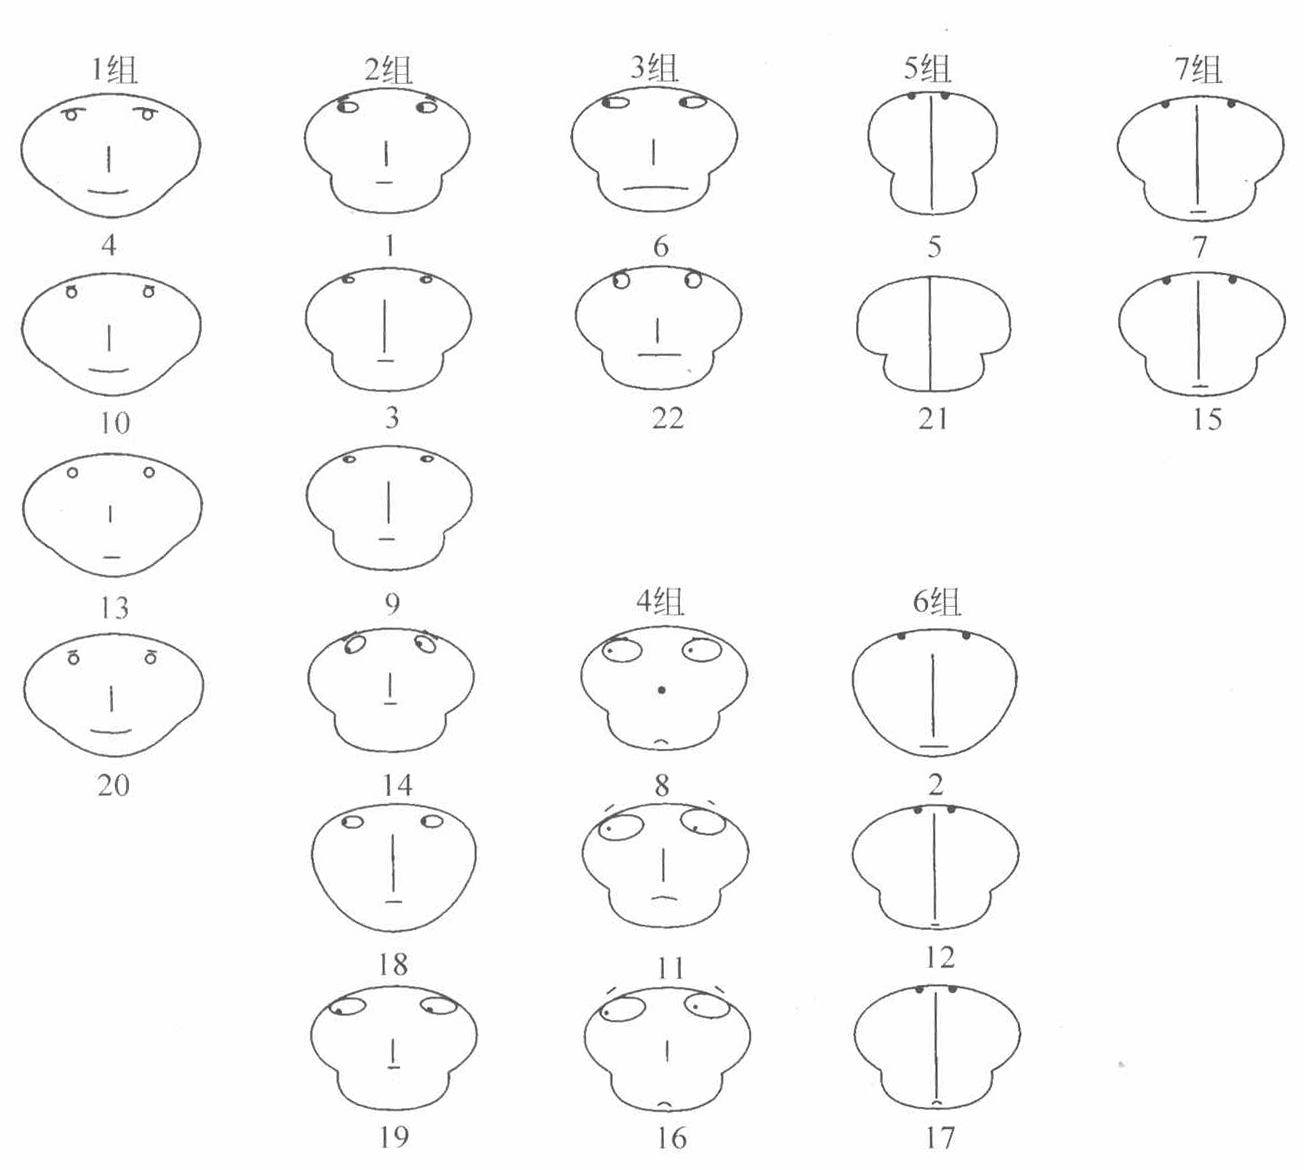
\includegraphics[width=110.4mm]{figs/fig_pg034_1.png}
\phantomsection\label{fig:1.17}\mvcap{图 1.17\quad 22 家公用事业公司的切尔诺夫脸}
\end{mvfigure}

\mvbold{例 1.13}\quad（利用切尔诺夫脸表示整个时期的变化）

\hyperref[fig:1.18]{图 1.18} 显示了切尔诺夫脸的额外的用法(参见文献[24]).在图中,脸被用来追踪一个公司在整个时期内的财务情况.如前面所说,每个脸部特征代表一个独立的经济指标,而这些指标的纵向变化是如此明显.

\begin{mvfigure}
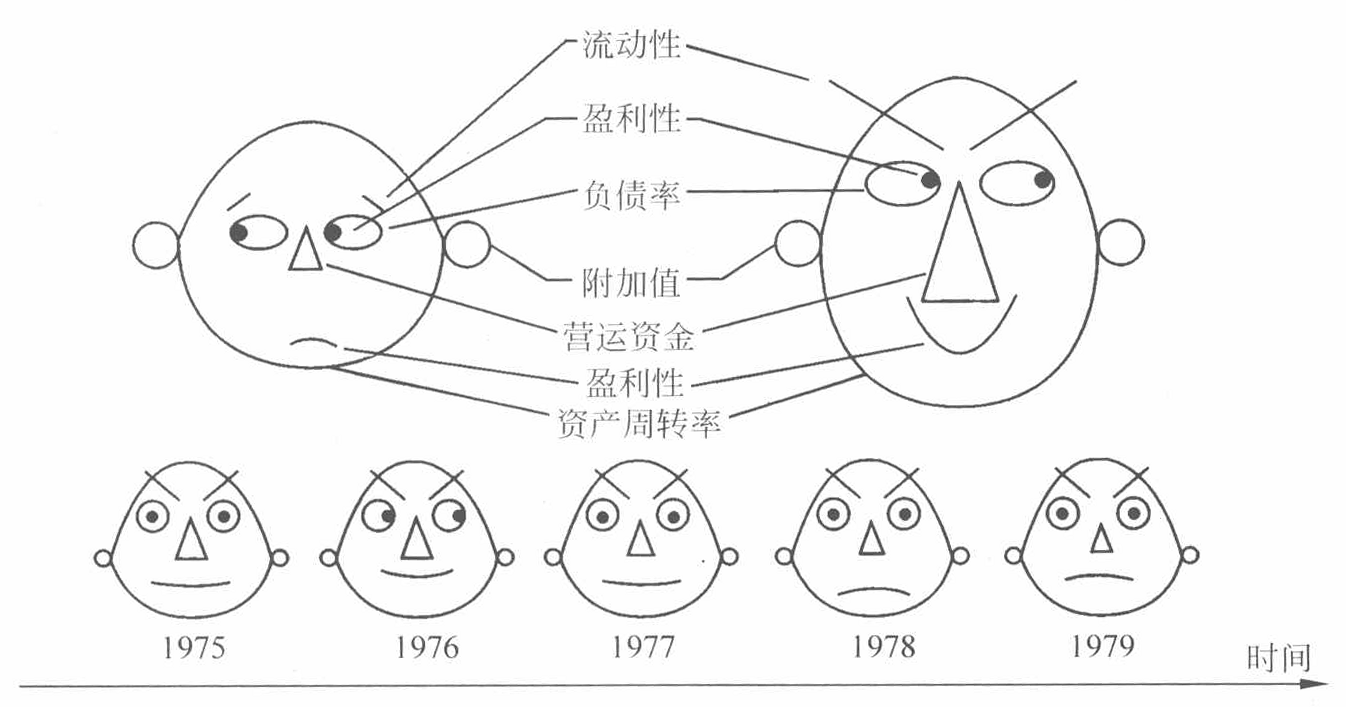
\includegraphics[width=114.0mm]{figs/fig_pg034_2.png}
\phantomsection\label{fig:1.18}\mvcap{图 1.18\quad 整个时期的切尔诺夫脸}
\end{mvfigure}

切尔诺夫脸也被用来显示多元观测值在二维空间中的差异.例如,二维空间的坐标轴可表示经度和纬度(地理位置),脸图可以表示几个美国城市的多元测量值.这一类的其他例子%

%% ===== pg-035 =====

% ---- pg-035 （书页 23） ----
见文献[30]中的讨论.

有许多灵巧的方法可以在二维空间中为多元数据作图. 我们已介绍其中几种, 利用先进的计算机作图是可能的而且几乎一定会取得更大的进展.

\section{距离}  % 原书 1.5
\phantomsection\label{sec:1.5}

尽管距离最初显得很难, 但大多数多元方法都基于简单的距离概念. 直线或欧几里德距离是我们所熟悉的. 如果我们考虑平面上的点 $P(x_1, x_2)$, 从 $P$ 点到原点 $O(0,0)$ 的直线距离 $d(O, P)$, 根据勾股定理, 是
\phantomsection\label{eq:1-9}
\begin{equation}
d(O, P) = \sqrt{x_1^2 + x_2^2} \tag{1-9}
\end{equation}
这种情况用\hyperref[fig:1.19]{图 1.19} 说明. 一般的, 若点 $P$ 有 $p$ 个坐标, 则 $P = (x_1, x_2, \cdots, x_p)$, $P$ 到原点 $O = (0, 0, \cdots, 0)$ 的直线距离为
\phantomsection\label{eq:1-10}
\begin{equation}
d(O, P) = \sqrt{x_1^2 + x_2^2 + \cdots + x_p^2} \tag{1-10}
\end{equation}
(参见第 2 章.)离原点有常数距离的平方(例如 $c^2$)的所有点 $(x_1, x_2, \cdots, x_p)$ 满足方程
\phantomsection\label{eq:1-11}
\begin{equation}
d^2(O, P) = x_1^2 + x_2^2 + \cdots + x_p^2 = c^2 \tag{1-11}
\end{equation}
由于这是一个超球面的方程(当 $p=2$ 时是个圆), 与原点等距的点都在超球面上.

坐标为 $P = (x_1, x_2, \cdots, x_p)$ 和 $Q = (y_1, y_2, \cdots, y_p)$ 的任意两个点 $P$ 和 $Q$ 的直线距离为
\phantomsection\label{eq:1-12}
\begin{equation}
d(P, Q) = \sqrt{(x_1 - y_1)^2 + (x_2 - y_2)^2 + \cdots + (x_p - y_p)^2} \tag{1-12}
\end{equation}

\begin{mvfigure}
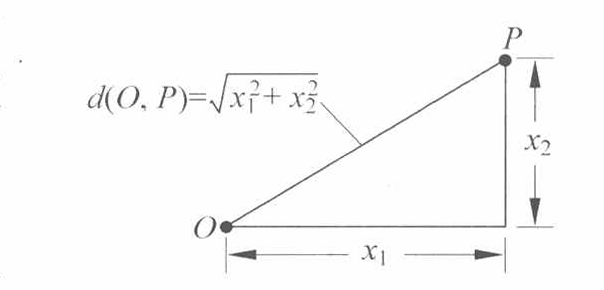
\includegraphics[width=51.2mm]{figs/fig_pg035_1.png}
\phantomsection\label{fig:1.19}\mvcap{图 1.19\quad 由勾股定理给出的距离}
\end{mvfigure}

直线或欧几里德距离对大多数的统计目的是不合用的. 这是因为每个坐标对于计算欧几里德距离起着相等的作用. 当坐标被用来表示不同随机波动的测量值时, 经常需要对那些可变性大的坐标加权大大少于对没有很大变化性的坐标的加权, 这就需要一种距离的不同的度量.

我们现在的目的是导出一个“统计的”距离. 这是由于考虑到变差的不同以及相关性的存在. 由于我们的选择取决于样本方差及协方差, 在这一点上我们用术语统计距离来将它和通常的欧几里德里距离区分开. 统计距离正是多元分析的基础.

开始, 我们把作 $p$ 维散布图的观测值集合看做是固定的. 根据这些我们将构造从原点到一点 $P = (x_1, x_2, \cdots, x_p)$ 的距离的度量. 在我们的论证中, $P$ 的坐标 $(x_1, x_2, \cdots, x_p)$ 可以变化以产生该点的不同位置. 然而, 确定距离的数据仍然保持固定.

\begin{mvfigure}
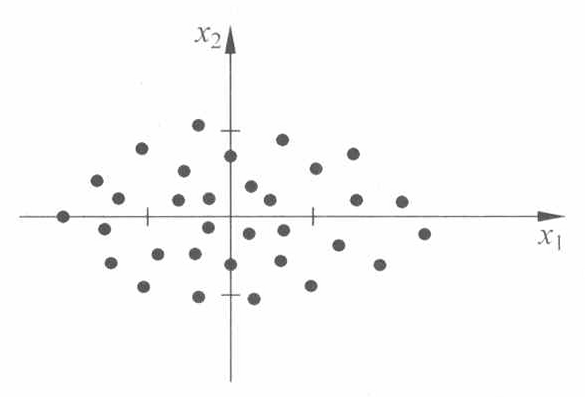
\includegraphics[width=49.5mm]{figs/fig_pg035_2.png}
\phantomsection\label{fig:1.20}\mvcap{图 1.20\quad 在 $x_1$ 方向上比在 $x_2$ 方向上变化性更大的散布图}
\end{mvfigure}

为举例说明, 假设我们有两个变量的 $n$ 对测量值, 称两个变量为 $x_1$ 和 $x_2$, 并假定变量 $x_1$ 的测量值关于 $x_2$ 的测量值独立地变化.\footnote{在这方面,“独立地”意指 $x_2$ 测量结果不能以任何的精确度预言来自 $x_1$ 的测量结果, 反之亦然.} 此外, 假设 $x_1$ 测量结果的可变性大于 $x_2$ 的测量结果的可变性. 数据的散布图看上去有点像\hyperref[fig:1.20]{图 1.20} 中的图片.

观察\hyperref[fig:1.20]{图 1.20}, 我们发现, 从原点出发向 $x_1$ 的方向给定的偏差的值不像从原点向 $x_2$ 方向等距离的值那样“惊人”或“不正常”. 这是因为 $x_1$ 方向内在的可变性大

%% ===== pg-036 =====

% ---- pg-036 （书页 24） ----

于 $x_2$ 方向的可变性.因此,大的 $x_1$ 坐标(用绝对值)不像大的 $x_2$ 坐标那样意外.当计算到原点的“距离”时,为 $x_2$ 坐标加权比为相同数值的 $x_1$ 坐标加权大一些,看起来是合理的.

接下来采用的方法是用样本标准差去除每个坐标.因此,被标准差除之后,得到“标准化”坐标 $x_1^* = x_1/\sqrt{s_{11}}$ 和 $x_2^* = x_2/\sqrt{s_{22}}$.现在这些标准化的坐标相互是在一个等同的基础上.在考虑变异性方面的不同后,我们利用标准欧几里德公式确定距离.

因此,从原点 $O = (0,0)$ 到点 $P = (x_1,x_2)$ 的统计距离可以由它的标准化坐标 $x_1^* = x_1/\sqrt{s_{11}}$ 和 $x_2^* = x_2/\sqrt{s_{22}}$ 计算出来.

\phantomsection\label{eq:1-13}
\begin{equation}
\begin{aligned}
d(O,P) &= \sqrt{(x_1^*)^2 + (x_2^*)^2} \\
&= \sqrt{\left(\frac{x_1}{\sqrt{s_{11}}}\right)^2 + \left(\frac{x_2}{\sqrt{s_{22}}}\right)^2} = \sqrt{\frac{x_1^2}{s_{11}} + \frac{x_2^2}{s_{22}}}
\end{aligned} \tag{1-13}
\end{equation}

比较\hyperref[eq:1-13]{式(1-13)}和\hyperref[eq:1-9]{式(1-9)},我们发现两式的不同是由于\hyperref[eq:1-13]{式(1-13)}中为 $x_1^2$ 和 $x_2^2$ 增加了权数 $k_1 = 1/s_{11}$ 和 $k_2 = 1/s_{22}$.注意,若样本方差是相同的, $k_1 = k_2$,则 $x_1^2$ 和 $x_2^2$ 将得到相同的权数.当权数相同时,忽略公因子,使用普通的欧几里德距离公式是很合适的.换言之,如果 $x_1$ 方向的变异性与 $x_2$ 方向的相同,并且 $x_1$ 值的变化不依赖于 $x_2$ 的值,欧几里德距离是适用的.

使用\hyperref[eq:1-13]{式(1-13)},我们看到所有到原点的距离的平方为常数 $c^2$ 的点,设坐标为 $(x_1,x_2)$,都满足

\phantomsection\label{eq:1-14}
\begin{equation}
\frac{x_1^2}{s_{11}} + \frac{x_2^2}{s_{22}} = c^2 \tag{1-14}
\end{equation}

\hyperref[eq:1-14]{式(1-14)}是一个椭圆方程,该椭圆以原点为中心,长轴和短轴分别与坐标轴重合.也就是说,\hyperref[eq:1-12]{式(1-12)}中统计距离的含义是,到原点距离为某常数的所有点的轨迹构成一椭圆.\hyperref[fig:1.21]{图 1.21} 表示了这种一般情况.

\begin{mvfigure}
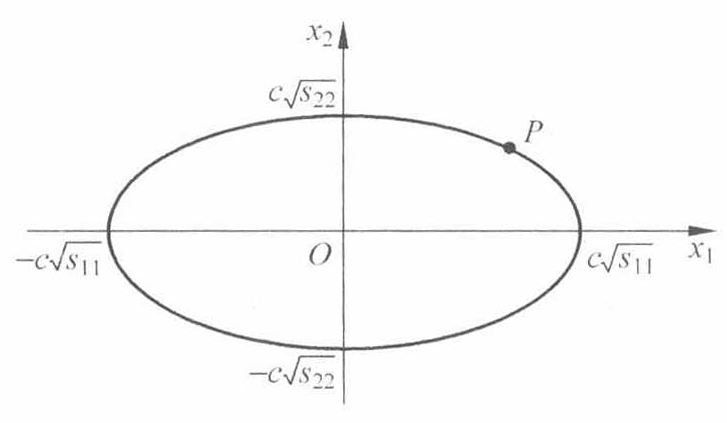
\includegraphics[width=61.6mm]{figs/fig_pg036_1.png}
\phantomsection\label{fig:1.21}\mvcap{图 1.21\quad 常数统计距离的椭圆}
\end{mvfigure}

$d^2(O,P) = x_1^2/s_{11} + x_2^2/s_{22} = c^2$

\mvbold{例 1.14}\quad （计算统计距离）

两个变量的一组测量值 $(x_1,x_2)$ 得出 $\bar{x}_1 = \bar{x}_2 = 0, s_{11} = 4$ 和 $s_{22} = 1$.假设测量值 $x_1$ 与测量值 $x_2$ 无关,即一对测量值中任一个量的变化都不依赖于另一个.由于样本方差不相等,我们用

\[
d^2(O,P) = \frac{x_1^2}{4} + \frac{x_2^2}{1}
\]

度量任意点 $P = (x_1,x_2)$ 到原点 $O = (0,0)$ 的距离平方.所有到原点固定距离为 1 的点 $(x_1,x_2)$ 满足方程

\[
\frac{x_1^2}{4} + \frac{x_2^2}{1} = 1
\]

距离原点 1 个单位的一些点的坐标如下表所示：

\begin{mvtable}
\begin{tabular}{ll|l|l}
\multicolumn{2}{c|}{坐标: $(x_1,x_2)$} & \multicolumn{2}{c}{距离: $\dfrac{x_1^2}{4} + \dfrac{x_2^2}{1} = 1$} \\
\hline
$(0,1)$ & & $\dfrac{0^2}{4} + \dfrac{1^2}{1} = 1$ & \\
$(0,-1)$ & & $\dfrac{0^2}{4} + \dfrac{(-1)^2}{1} = 1$ & \\
$(2,0)$ & & $\dfrac{2^2}{4} + \dfrac{0^2}{1} = 1$ & \\
$(1,\sqrt{3}/2)$ & & $\dfrac{1^2}{4} + \dfrac{(\sqrt{3}/2)^2}{1} = 1$ & \\
\end{tabular}
\end{mvtable}

方程 $x_1^2/4 + x_2^2/1 = 1$ 的图形是一个中心在 $(0,0)$ 的椭圆,它的长轴沿着 $x_1$ 坐标轴,短轴则

%% ===== pg-037 =====

% ---- pg-037 （书页 25） ----

沿着 $x_2$ 坐标轴.长轴与短轴的半轴长分别为 $\sqrt{4} = 2$ 和 $\sqrt{1} = 1$.单位距离的椭圆在\hyperref[fig:1.22]{图 1.22} 中画出.椭圆上的所有点到原点有相等的统计距离.在此例中,距离为 1. \ $\blacksquare$

\begin{mvfigure}
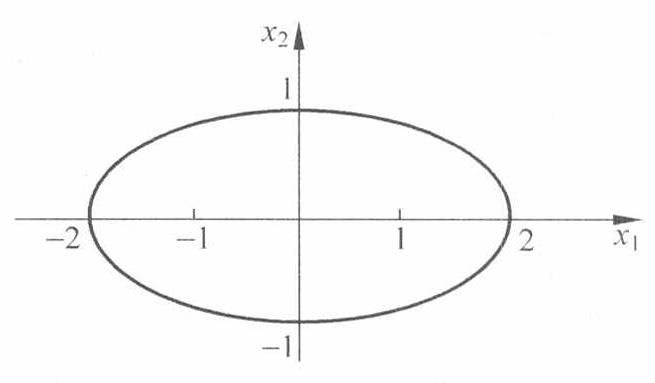
\includegraphics[width=55.5mm]{figs/fig_pg037_1.png}
\phantomsection\label{fig:1.22}\mvcap{图 1.22\quad 单位距离的椭圆}
\vspace{2pt}
$\dfrac{x_1^2}{4} + \dfrac{x_2^2}{1} = 1$
\end{mvfigure}

\hyperref[eq:1-13]{式(1-13)}可以加以引申来适应计算任意一点 $P = (x_1,x_2)$ 到任何固定点 $Q = (y_1,y_2)$ 的统计距离.如果我们假定一个变量坐标的变化独立于另一个,则 $P$ 到 $Q$ 的距离为

\phantomsection\label{eq:1-15}
\begin{equation}
d(P,Q) = \sqrt{\frac{(x_1 - y_1)^2}{s_{11}} + \frac{(x_2 - y_2)^2}{s_{22}}} \tag{1-15}
\end{equation}

这一统计距离公式可直接推广到大于二维的空间中.令点 $P$ 和 $Q$ 含有 $p$ 个坐标,即 $P = (x_1,x_2,\cdots,x_p)$ 和 $Q = (y_1,y_2,\cdots,y_p)$.假设 $Q$ 是一固定点[它可以是原点 $O = (0,0,\cdots,0)$]且变量坐标的变化相互独立.令 $s_{11},s_{22},\cdots,s_{pp}$ 分别是由 $x_1,x_2,\cdots,x_p$ 的 $n$ 个测量值构造的样本方差,则从 $P$ 到 $Q$ 的统计距离是

\phantomsection\label{eq:1-16}
\begin{equation}
d(P,Q) = \sqrt{\frac{(x_1 - y_1)^2}{s_{11}} + \frac{(x_2 - y_2)^2}{s_{22}} + \cdots + \frac{(x_p - y_p)^2}{s_{pp}}} \tag{1-16}
\end{equation}

所有到 $Q$ 的距离平方为某定值的点 $P$ 分布在一个超椭球面上,其中心为 $Q$,长轴及短轴平行于坐标轴.我们应注意下列几点:

1. 要得到 $P$ 到原点 $O$ 的距离,需对\hyperref[eq:1-16]{式(1-16)}设 $y_1 = y_2 = \cdots = y_p = 0$.
2. 如果 $s_{11} = s_{22} = \cdots = s_{pp}$,\hyperref[eq:1-12]{式(1-12)}中的欧几里德距离公式是适用的.

\begin{mvfigure}
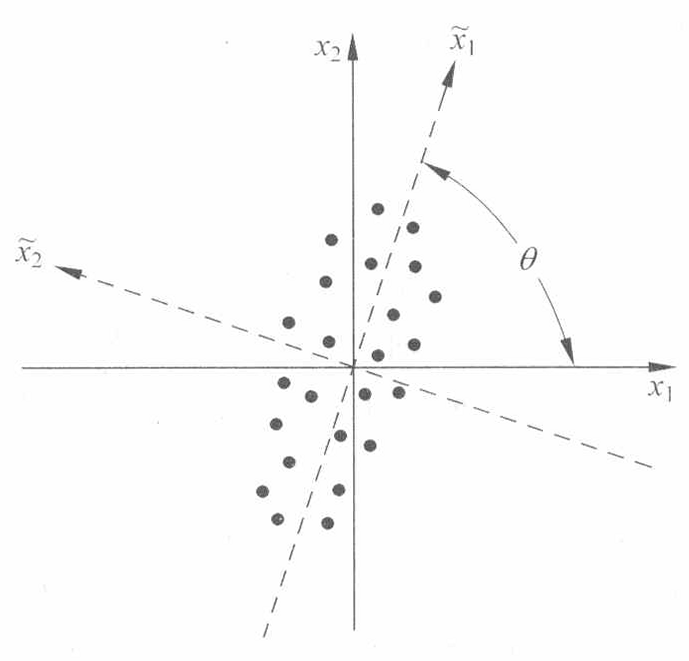
\includegraphics[width=58.3mm]{figs/fig_pg037_2.png}
\phantomsection\label{fig:1.23}\mvcap{图 1.23\quad 对正相关测量值和一个\\旋转坐标系的散布图}
\end{mvfigure}

由于假设坐标是独立的,\hyperref[eq:1-16]{式(1-16)}中的距离公式仍未包括我们将要遇到的许多重要情况.\hyperref[fig:1.23]{图 1.23} 的散布图描述了一个二维空间中 $x_1$ 的测量值的变化依赖于 $x_2$ 的情况.实际上,这一对变量 $(x_1,x_2)$ 的坐标显示出同大或同小的趋势,并且样本相关系数是正的.此外, $x_2$ 方向的可变性大于 $x_1$ 方向的可变性.

当 $x_1$ 方向的可变性与 $x_2$ 方向的可变性不同并且变量 $x_1$ 与 $x_2$ 相关时,什么是有意义的距离的度量？实际上,只要我们用正确的方法观察事物,我们就可以利用已介绍过的方法.从\hyperref[fig:1.23]{图 1.23},我们发现如果在保持散布不变的基础上,将原始的坐标系旋转 $\theta$ 角并标出旋转过的坐标轴 $\tilde{x}_1$ 和 $\tilde{x}_2$,在新坐标轴下的散布图看起来非常像\hyperref[fig:1.20]{图 1.20} 中所画的.(你可以将书旋转,使 $\tilde{x}_1$ 和 $\tilde{x}_2$ 轴回到它们通常的位置.)假设我们用 $\tilde{x}_1$ 和 $\tilde{x}_2$ 坐标计算样本方差,用\hyperref[eq:1-13]{式(1-13)}度量距离,即,根据 $\tilde{x}_1$ 和 $\tilde{x}_2$,我们把点 $P = (\tilde{x}_1,\tilde{x}_2)$ 到原点 $O = (0,0)$ 的距离定义为

\phantomsection\label{eq:1-17}
\begin{equation}
d(O,P) = \sqrt{\frac{\tilde{x}_1^2}{\tilde{s}_{11}} + \frac{\tilde{x}_2^2}{\tilde{s}_{22}}} \tag{1-17}
\end{equation}

其中 $\tilde{s}_{11}$ 和 $\tilde{s}_{22}$ 分别表示由 $\tilde{x}_1$ 和 $\tilde{x}_2$ 的测量值计算出的样本方差.

%% ===== pg-038 =====

% ---- pg-038 （书页 26） ----

原始坐标 $(x_1, x_2)$ 与旋转后所得坐标 $(\tilde{x}_1, \tilde{x}_2)$ 之间的关系如下
\[
\tilde{x}_1 = x_1\cos(\theta) + x_2\sin(\theta)
\]
\phantomsection\label{eq:1-18}
\begin{equation}
\tilde{x}_2 = -x_1\sin(\theta) + x_2\cos(\theta) \tag{1-18}
\end{equation}
根据\hyperref[eq:1-18]{式(1-18)} 给出的关系式，我们可以替换\hyperref[eq:1-17]{式(1-17)} 中的 $\tilde{x}_1$ 和 $\tilde{x}_2$，用原来的坐标来表示
距离.

经过一些简单的代数变换，从 $P=(\tilde{x}_1, \tilde{x}_2)$ 到原点 $O=(0, 0)$ 的距离可以用 $P$ 的原始坐标
$x_1$ 和 $x_2$ 表示为
\phantomsection\label{eq:1-19}
\begin{equation}
d(O, P) = \sqrt{a_{11}x_1^2 + 2a_{12}x_1x_2 + a_{22}x_2^2} \tag{1-19}
\end{equation}
其中 $a$ 为使得 $x_1$ 和 $x_2$ 取所有可能值时，距离都为非负的数. 这里，$a_{11}, a_{12}$ 和 $a_{22}$ 由角 $\theta$ 决定，
且 $s_{11}, s_{12}$ 和 $s_{22}$ 是由原始数据计算出来的. \footnote{具体地，
\[
a_{11} = \frac{\cos^2(\theta)}{\cos^2(\theta)s_{11} + 2\sin(\theta)\cos(\theta)s_{12} + \sin^2(\theta)s_{22}} + \frac{\sin^2(\theta)}{\cos^2(\theta)s_{22} - 2\sin(\theta)\cos(\theta)s_{12} + \sin^2(\theta)s_{11}}
\]
\[
a_{22} = \frac{\sin^2(\theta)}{\cos^2(\theta)s_{11} + 2\sin(\theta)\cos(\theta)s_{12} + \sin^2(\theta)s_{22}} + \frac{\cos^2(\theta)}{\cos^2(\theta)s_{22} - 2\sin(\theta)\cos(\theta)s_{12} + \sin^2(\theta)s_{11}}
\]
\[
a_{12} = \frac{\cos(\theta)\sin(\theta)}{\cos^2(\theta)s_{11} + 2\sin(\theta)\cos(\theta)s_{12} + \sin^2(\theta)s_{22}} - \frac{\sin(\theta)\cos(\theta)}{\cos^2(\theta)s_{22} - 2\sin(\theta)\cos(\theta)s_{12} + \sin^2(\theta)s_{11}}
\]} 此处 $a_{11}, a_{12}$ 和 $a_{22}$
的特定形式并不重要的. 重要的是非零相关系数 $r_{12}$ 所需要的交叉乘积项 $2a_{12}x_1x_2$ 的出现.

比较\hyperref[eq:1-13]{式(1-13)} 与\hyperref[eq:1-19]{式(1-19)}，\hyperref[eq:1-13]{式(1-13)} 可看做是\hyperref[eq:1-19]{式(1-19)} 在 $a_{11} = 1/s_{11}, a_{22} = 1/s_{22}$ 且 $a_{12} = 0$
时的特殊情况.

一般的，在变量相关的情况下，从固定点 $Q=(y_1, y_2)$ 到点 $P=(x_1, x_2)$ 的统计距离的一般
形式为
\phantomsection\label{eq:1-20}
\begin{equation}
d(P, Q) = \sqrt{a_{11}(x_1 - y_1)^2 + 2a_{12}(x_1 - y_1)(x_2 - y_2) + a_{22}(x_2 - y_2)^2} \tag{1-20}
\end{equation}
且当 $a_{11}, a_{12}$ 及 $a_{22}$ 为已知时，距离总是可计算出来的. 此外，所有与 $Q$ 的距离平方为常数 $c^2$ 的
点 $P=(x_1, x_2)$ 的坐标满足
\phantomsection\label{eq:1-21}
\begin{equation}
a_{11}(x_1 - y_1)^2 + 2a_{12}(x_1 - y_1)(x_2 - y_2) + a_{22}(x_2 - y_2)^2 = c^2 \tag{1-21}
\end{equation}

\begin{mvfigure}
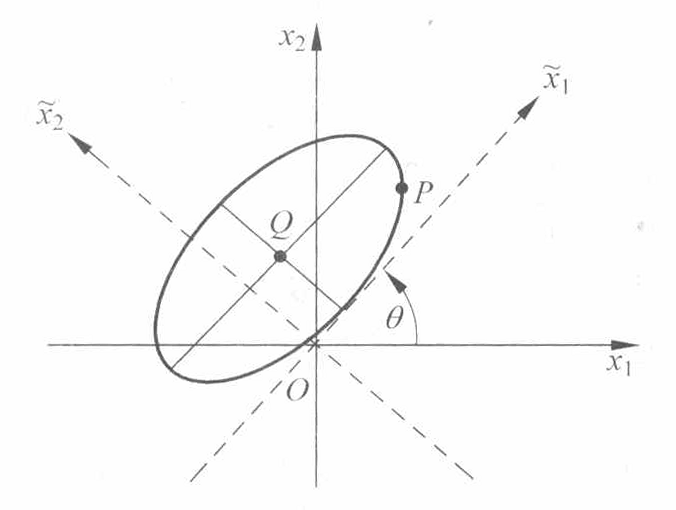
\includegraphics[width=57.3mm]{figs/fig_pg038_1.png}
\phantomsection\label{fig:1.24}\mvcap{图 1.24\quad 到点 $Q$ 为常数距离的点的椭圆}
\end{mvfigure}

按照定义，这是一个中心在 $Q$ 的椭圆方程. 方程的
图形如\hyperref[fig:1.24]{图 1.24} 所示，长轴与短轴被标出来了，它
们分别平行于 $\tilde{x}_1$ 轴与 $\tilde{x}_2$ 轴. 由于选择了脚注中的
$a_{11}, a_{12}$ 及 $a_{22}$，$\tilde{x}_1$ 和 $\tilde{x}_2$ 轴相对于 $x_1$ 和 $x_2$ 轴成 $\theta$ 角.

\hyperref[eq:1-19]{式(1-19)} 及\hyperref[eq:1-20]{式(1-20)} 的距离公式可直接推广
到 $p$ 维空间. 设 $P=(x_1, x_2, \cdots, x_p)$ 为一点，其坐
标表示一组相关且服从内在可变性的变量. $O=$
$(0, 0, \cdots, 0)$ 表示原点，$Q=(y_1, y_2, \cdots, y_p)$ 为一指
定的固定点，则 $P$ 到 $O$ 和 $P$ 到 $Q$ 的距离具有一般
形式
\phantomsection\label{eq:1-22}
\begin{equation}
d(O, P) = \sqrt{a_{11}x_1^2 + a_{22}x_2^2 + \cdots + a_{pp}x_p^2 + 2a_{12}x_1x_2 + 2a_{13}x_1x_3 + \cdots + 2a_{p-1,p}x_{p-1}x_p} \tag{1-22}
\end{equation}

%% ===== pg-039 =====

% ---- pg-039 （书页 27） ----

和

\phantomsection\label{eq:1-23}
\begin{equation}
\begin{aligned}
d(P, Q) &= [a_{11}(x_1 - y_1)^2 + a_{22}(x_2 - y_2)^2 + \cdots + a_{pp}(x_p - y_p)^2 + 2a_{12}(x_1 - y_1)(x_2 - y_2) \\
&\quad + 2a_{13}(x_1 - y_1)(x_3 - y_3) + \cdots + 2a_{p-1,p}(x_{p-1} - y_{p-1})(x_p - y_p)]^{1/2}
\end{aligned} \tag{1-23}
\end{equation}
其中 $a$ 为使得距离总为非负的数. \footnote{式 (1-22) 和\hyperref[eq:1-23]{式(1-23)} 中的距离平方的代数表达式被称为二次型，具体被称为正定二次型. 用矩阵以简单形式表示这些二次型是可能的，我们将在 2.3 节中讲述.}

我们注意到\hyperref[eq:1-22]{式(1-22)} 及\hyperref[eq:1-23]{式(1-23)} 中的距离完全由系数（权数）$a_{ik}, i = 1, 2, \cdots, p, k = 1, 2, \cdots, p$，决定. 这些系数可在一矩形阵列中表示出来
\phantomsection\label{eq:1-24}
\begin{equation}
\begin{bmatrix}
a_{11} & a_{12} & \cdots & a_{1p} \\
a_{12} & a_{22} & \cdots & a_{2p} \\
\vdots & \vdots & & \vdots \\
a_{1p} & a_{2p} & \cdots & a_{pp}
\end{bmatrix} \tag{1-24}
\end{equation}
其中系数 $a_{ik} (i \neq k)$ 出现了两次，这是因为它们在距离公式中被乘了 2. 因此，这个阵列中的元素确定距离函数. $a_{ik}$ 不能是任意数值，它们必须使得计算出的每一对点的距离都为非负的数（参见练习 1.10）\footnote{式(1-22)和\hyperref[eq:1-23]{式(1-23)}中的距离平方的代数表达式被称为二次型，具体被称为正定二次型. 用矩阵以一简单形式表示这些二次型是可能的，我们将在 2.3 节中讲述.}.

由\hyperref[eq:1-22]{式(1-22)} 和\hyperref[eq:1-23]{式(1-23)} 计算出的定常数距离的轮廓线是一超椭球面，当 $p = 3$ 时，超椭球面像一个橄榄球；超过三维时，其形象化是不可能的.

\begin{mvfigure}
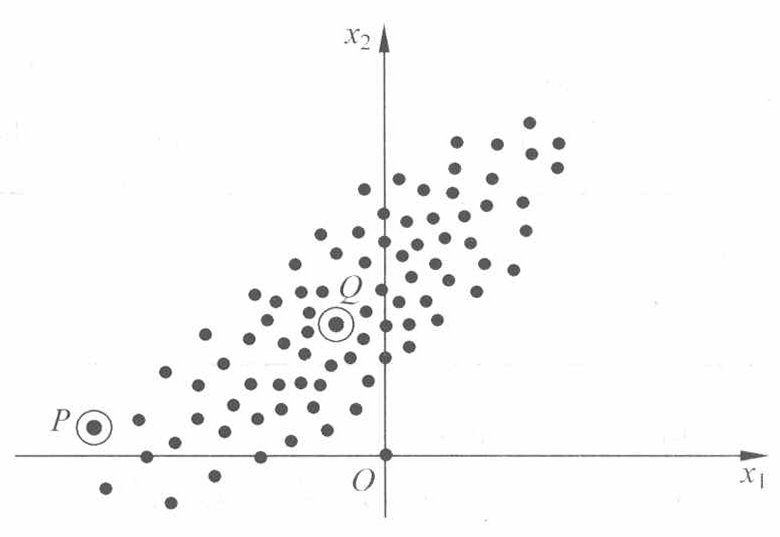
\includegraphics[width=66.1mm]{figs/fig_pg039_1.png}
\phantomsection\label{fig:1.25}\mvcap{图 1.25\quad 相对于点 $P$ 和原点的一组点}
\end{mvfigure}

\hyperref[fig:1.25]{图 1.25} 启发性地说明了需要考虑统计距离而不是欧几里德距离. \hyperref[fig:1.25]{图 1.25} 描述了重心（样本均值）在点 $Q$ 的一组点. 考虑从点 $Q$ 到点 $P$ 和到原点 $O$ 的欧几里德距离. $Q$ 到 $P$ 的欧几里德距离大于 $Q$ 到 $O$ 的欧几里德距离. 然而，$P$ 点比原点显得更像是属于这一组点内的点. 如果我们考虑到这一组点的可变性，并用\hyperref[eq:1-20]{式(1-20)} 的统计距离来度量距离，则 $Q$ 距离 $P$ 比距离 $O$ 要近. 这个结果看来合理地给出了散布的本质.

还有一些其他的距离的度量方法（参见练习 1.12）. 有时，考虑不涉及圆或椭圆的距离是有益的. $P$ 和 $Q$ 两点之间的任何距离度量 $d(P, Q)$ 如果满足下面的性质，都是有效的，其中 $R$ 是任一个其他中间点：
\phantomsection\label{eq:1-25}
\begin{equation}
\begin{aligned}
&d(P, Q) = d(Q, P) \\
&d(P, Q) > 0, \text{若 } P \neq Q \\
&d(P, Q) = 0, \text{若 } P = Q \\
&d(P, Q) \leqslant d(P, R) + d(R, Q) \quad \text{（三角不等式）}
\end{aligned} \tag{1-25}
\end{equation}

\section{最终评注}  % 原书 1.6
\phantomsection\label{sec:1.6}

我们试图推动多元分析的研究，并为您提供一些组织、概括及展示数据的基本而重要的

%% ===== pg-040 =====

% ---- pg-040 （书页 28） ----

方法. 此外，还介绍了一个一般性的距离概念，在后面的章节将会反复用到它.

{\large\bfseries 练习}

\mvbold{1.1} 考虑\hyperref[fig:1.1]{图 1.1} 中所画的 7 对测量值 $(x_1, x_2)$：

\begin{mvtable}
\begin{tabular}{lccccccc}
\toprule
$x_1$ & 3 & 4 & 2 & 6 & 8 & 2 & 5 \\
$x_2$ & 5 & 5.5 & 4 & 7 & 10 & 5 & 7.5 \\
\bottomrule
\end{tabular}
\end{mvtable}

计算样本均值 $\bar{x}_1$ 和 $\bar{x}_2$，样本方差 $s_{11}$ 和 $s_{22}$ 及样本协方差 $s_{12}$.

\mvbold{1.2} 一家晨报列出一种外国小轿车的二手车价格，车龄 $x_1$ 以年度量，销售价格 $x_2$ 以千美元度量：

\begin{mvtable}
\begin{tabular}{lccccccccccc}
\toprule
$x_1$ & 1 & 2 & 3 & 3 & 4 & 5 & 6 & 8 & 9 & 11 \\
$x_2$ & 18.95 & 19.00 & 17.95 & 15.54 & 14.00 & 12.95 & 8.94 & 7.49 & 6.00 & 3.99 \\
\bottomrule
\end{tabular}
\end{mvtable}

(a) 作数据的散布图及边缘点图.

(b) 根据散布图推断样本协方差的正负号.

(c) 计算样本均值 $\bar{x}_1$ 和 $\bar{x}_2$ 及样本方差 $s_{11}$ 和 $s_{22}$，计算样本协方差 $s_{12}$ 和样本相关系数 $r_{12}$. 解释这些参数.

(d) 利用\hyperref[eq:1-8]{式(1-8)} 写出样本均值阵列 $\bar{\bm{x}}$，样本方差-协方差阵列 $\bm{S}_n$ 和样本相关阵列 $\bm{R}$.

\mvbold{1.3} 下面是变量 $x_1, x_2$ 和 $x_3$ 的 5 个测量值：

\begin{mvtable}
\begin{tabular}{lccccc}
\toprule
$x_1$ & 9 & 2 & 6 & 5 & 8 \\
$x_2$ & 12 & 8 & 6 & 4 & 10 \\
$x_3$ & 3 & 4 & 0 & 2 & 1 \\
\bottomrule
\end{tabular}
\end{mvtable}

求阵列 $\bar{\bm{x}}, \bm{S}_n$ 和 $\bm{R}$.

\mvbold{1.4} 全球 10 大公司的收益数据如下：

\begin{mvtable}
\mvtabcap{全球 10 大公司 \hfill （10 亿美元）}
\begin{tabular}{lrrr}
\toprule
公司 & $x_1 = $ 销售总额 & $x_2 = $ 利润 & $x_3 = $ 资产 \\
\midrule
花旗集团 & 108.28 & 17.05 & 1 484.10 \\
通用电气 & 152.36 & 16.59 & 750.33 \\
美国国际集团 & 95.04 & 10.91 & 766.42 \\
美洲银行 & 65.45 & 14.14 & 1 110.46 \\
汇丰集团 & 62.97 & 9.52 & 1 031.29 \\
埃克森美孚 & 263.99 & 25.33 & 195.26 \\
皇家荷兰壳牌 & 265.19 & 18.54 & 193.83 \\
英国石油 & 285.06 & 15.73 & 191.11 \\
荷兰国际 & 92.01 & 8.10 & 1 175.16 \\
丰田摩托 & 165.68 & 11.13 & 211.15 \\
\bottomrule
\end{tabular}
\end{mvtable}

{\zihao{6} 资料来源：www. Forbes. com 及福布斯集团的《福布斯》杂志 (2005 年 4 月 18 日).}

(a) 为变量 $x_1$ 和 $x_2$ 作散布图及边缘点图，并加以解释.

(b) 计算 $\bar{x}_1, \bar{x}_2, s_{11}, s_{22}, s_{12}$ 和 $r_{12}$. 解释 $r_{12}$.

%% ===== pg-041 =====

% ---- pg-041 （书页 29） ----

\mvbold{1.5} 利用练习 1.4 中的数据

(a) 画出 $(x_2, x_1)$ 和 $(x_1, x_2)$ 的散布图和边缘点图. 解释这些图形.

(b) 计算 $(x_1, x_2, x_3)$ 的阵列 $\bar{\bm{x}}, \bm{S}$ 和 $\bm{R}$.

\mvbold{1.6} \hyperref[tab:1.5]{表 1.5} 中的数据是对洛杉矶地区空气污染变量的 42 个测量值的记录，这些测量值是在不同日子的中午 12 点采集的（可参见 www. prenhall. com/statistics 的空气污染数据）.

\begin{mvtable}
\phantomsection\label{tab:1.5}\mvtabcap{表 1.5\quad 空气污染数据}
\begin{longtable}{rrrrrrrr}\toprule
风 $(x_1)$ & 日光辐射 $(x_2)$ & $\mathrm{CO}(x_3)$ & $\mathrm{NO}(x_4)$ & $\mathrm{NO}_2(x_5)$ & $\mathrm{O}_3(x_6)$ & $\mathrm{HC}(x_7)$ \\
\midrule
\endfirsthead
\multicolumn{7}{c}{\zihao{6}续表}\\
\toprule
风 $(x_1)$ & 日光辐射 $(x_2)$ & $\mathrm{CO}(x_3)$ & $\mathrm{NO}(x_4)$ & $\mathrm{NO}_2(x_5)$ & $\mathrm{O}_3(x_6)$ & $\mathrm{HC}(x_7)$ \\
\midrule
\endhead
\bottomrule
\endlastfoot

8 & 98 & 7 & 2 & 12 & 8 & 2 \\
7 & 107 & 4 & 3 & 9 & 5 & 3 \\
7 & 103 & 4 & 3 & 5 & 6 & 3 \\
10 & 88 & 5 & 2 & 8 & 15 & 4 \\
6 & 91 & 4 & 2 & 8 & 10 & 3 \\
8 & 90 & 5 & 2 & 12 & 12 & 4 \\
9 & 84 & 7 & 4 & 12 & 15 & 5 \\
5 & 72 & 6 & 4 & 21 & 14 & 4 \\
7 & 82 & 5 & 1 & 11 & 11 & 3 \\
8 & 64 & 5 & 2 & 13 & 9 & 4 \\
6 & 71 & 5 & 4 & 10 & 3 & 3 \\
6 & 91 & 4 & 2 & 12 & 7 & 3 \\
7 & 72 & 7 & 4 & 18 & 10 & 3 \\
10 & 70 & 4 & 2 & 11 & 7 & 3 \\
10 & 72 & 4 & 1 & 8 & 10 & 3 \\
9 & 77 & 4 & 1 & 9 & 10 & 3 \\
8 & 76 & 4 & 1 & 7 & 7 & 3 \\
8 & 71 & 5 & 3 & 16 & 4 & 4 \\
9 & 67 & 4 & 2 & 13 & 2 & 3 \\
9 & 69 & 3 & 3 & 9 & 5 & 3 \\
10 & 62 & 5 & 3 & 14 & 4 & 3 \\
9 & 88 & 4 & 2 & 7 & 6 & 3 \\
8 & 80 & 4 & 2 & 13 & 11 & 4 \\
5 & 30 & 3 & 3 & 5 & 2 & 3 \\
6 & 83 & 5 & 1 & 10 & 23 & 4 \\
8 & 84 & 3 & 2 & 7 & 6 & 3 \\
6 & 78 & 4 & 2 & 11 & 11 & 3 \\
8 & 79 & 2 & 1 & 7 & 10 & 3 \\
6 & 62 & 4 & 3 & 9 & 8 & 3 \\
10 & 37 & 3 & 1 & 7 & 2 & 3 \\
8 & 71 & 4 & 1 & 10 & 7 & 3 \\
7 & 52 & 4 & 1 & 12 & 8 & 4 \\
5 & 48 & 6 & 5 & 8 & 4 & 3 \\
6 & 75 & 4 & 1 & 10 & 24 & 3 \\
10 & 35 & 4 & 1 & 6 & 9 & 2 \\
8 & 85 & 4 & 1 & 9 & 10 & 2 \\
5 & 86 & 3 & 1 & 6 & 12 & 2 \\
5 & 86 & 7 & 2 & 13 & 18 & 3 \\
7 & 79 & 7 & 4 & 9 & 25 & 2 \\
7 & 79 & 5 & 2 & 8 & 6 & 2 \\
6 & 68 & 6 & 2 & 11 & 14 & 3 \\
8 & 40 & 4 & 3 & 6 & 5 & 2 \\
\end{longtable}
\end{mvtable}

{\zihao{6} 资料来源：数据经 G. C. Tiao 教授许可使用.}

%% ===== pg-042 =====

% ---- pg-042 （书页 30） ----

(a) 为所有变量作边缘点图.

(b) 构造阵列 $\bar{\bm{x}}, \bm{S}$, 和 $\bm{R}$ 并对 $\bm{R}$ 中元素作解释.

\mvbold{1.7} 下面给出对 $p = 2$ 个变量的 $n = 3$ 个观测值：

变量 1：\quad $x_{11} = 2$ \quad $x_{21} = 3$ \quad $x_{31} = 4$

变量 2：\quad $x_{12} = 1$ \quad $x_{22} = 2$ \quad $x_{32} = 4$

(a) 为每对观测值在二维“变量空间”作图，即构造数据的二维散布图.

(b) 在三维“项目空间”中将数据作为两点标出.

\mvbold{1.8} 用\hyperref[eq:1-12]{式(1-12)} 的欧几里德距离公式，取 $p = 2$ 及用\hyperref[eq:1-20]{式(1-20)} 的统计距离公式，取 $a_{11} = 1/3, a_{22} = 4/27, a_{12} = 1/9$. 计算点 $P = (-1, 1)$ 到点 $Q = (1, 0)$ 的距离. 画出到点 $Q$ 的统计距离平方为常数 1 的点的轨迹.

\mvbold{1.9} 考虑下面两个变量 $x_1$ 和 $x_2$ 的 8 对测量值：

\begin{mvtable}
\begin{tabular}{lcccccccc}
\toprule
$x_1$ & $-6$ & $-3$ & $-2$ & 1 & 2 & 5 & 6 & 8 \\
$x_2$ & $-2$ & $-3$ & 1 & $-1$ & 2 & 1 & 5 & 3 \\
\bottomrule
\end{tabular}
\end{mvtable}

(a) 画出数据的散布图，并计算 $s_{11}, s_{22}$ 及 $s_{12}$.

(b) 假定将原始坐标轴旋转角度 $\theta = 26^\circ$ [已知 $\cos(26^\circ) = 0.899$ 和 $\sin(26^\circ) = 0.438$]. 利用\hyperref[eq:1-18]{式(1-18)} 计算与变量 $x_1, \tilde{x}_2$ 对应的测量值.

(c) 根据 (b) 中求出的 $\tilde{x}_1, \tilde{x}_2$ 的测量值，计算样本方差 $\tilde{s}_{11}$ 及 $\tilde{s}_{22}$.

(d) 设一对新的测量值 $(x_1, x_2) = (4, -2)$. 用\hyperref[eq:1-18]{式(1-18)} 将它们变换为 $\tilde{x}_1$ 和 $\tilde{x}_2$ 的测量值，并用\hyperref[eq:1-17]{式(1-17)} 计算原点 $O = (0, 0)$ 到新点 $P = (\tilde{x}_1, \tilde{x}_2)$ 的距离 $d(O, P)$.

注意：需要用到 (c) 中求出的 $\tilde{s}_{11}$ 和 $\tilde{s}_{22}$.

(e) 用\hyperref[eq:1-19]{式(1-19)} 及脚注 2 中给出的关于 $a_{11}, a_{12}$ 及 $a_{22}$ 的表达式，计算点 $P = (4, -2)$ 到原点 $O = (0, 0)$ 的距离.

注意：需用到 (a) 中求出的 $s_{11}, s_{22}$ 及 $s_{12}$.

将这一计算出的距离和 (d) 中用 $\tilde{x}_1$ 和 $\tilde{x}_2$ 的值算出的距离进行比较（在舍入误差范围内，数值应是相同的）.

\mvbold{1.10} 下面的距离函数对于计算从原点出发的距离是否有效？试解释.

(a) $x_1^2 + 4x_2^2 + x_1x_2 = $(距离)$^2$

(b) $x_1^2 - 2x_2^2 = $(距离)$^2$

\mvbold{1.11} 设 $a_{11} = 4, a_{22} = 1$ 和 $a_{12} = -1$，证明\hyperref[eq:1-20]{式(1-20)} 定义的距离满足\hyperref[eq:1-25]{式(1-25)} 中的前三个条件（三角不等式较难证明）.

\mvbold{1.12} 定义从点 $P = (x_1, x_2)$ 到原点 $O = (0, 0)$ 的距离为
\[
d(O, P) = \max\{|x_1|, |x_2|\}
\]

(a) 计算从点 $P = (-3, 4)$ 到原点的距离.

(b) 画出到原点的距离平方为 1 的点的轨迹.

(c) 将上述距离公式推广到 $p$ 维空间中的点.

\mvbold{1.13} 一个大城市的主要道路被设计成网格形，如下图所示. 街道 1 至街道 5 的方向为从北至南 (NS)，街道 A 至街道 E 方向为从东至西 (EW). 假设在交点 $(A, 2), (E, 3)$ 和 $(C, 5)$ 上有零售商店. 又假定在一条街上两个交点之间的距离不论是南北方向还是东西方向都为 1 个单位. 网格上任何两个交点（点）间的距离称为“城市街区”距离. （例如交点 $(D, 1)$ 和 $(C, 2)$ 间的距离，我们可以称之为 $d((D, 1), (C, 2))$，可以这样算出 $d((D, 1), (C, 2)) = d((D, 1)$，

%% ===== pg-043 =====

% ---- pg-043 （书页 31） ----

$(D,2))+d((D,2),(C,2))=1+1=2$, 或是 $d((D,1),(C,2))=d((D,1),(C,1))+d((C,1),%
(C,2))=1+1=2$. )

\begin{mvfigure}
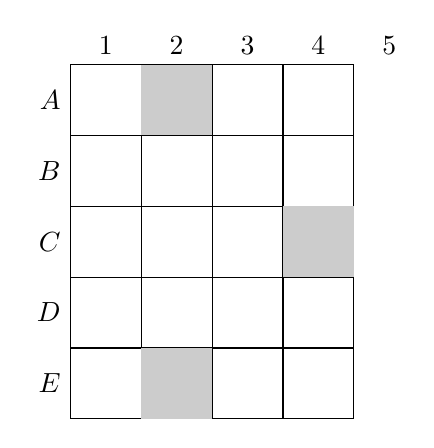
\begin{tikzpicture}[scale=0.9]
\draw[step=1cm] (0,0) grid (4,5);
\fill[gray!40] (1,4) rectangle (2,5);
\fill[gray!40] (3,2) rectangle (4,3);
\fill[gray!40] (1,0) rectangle (2,1);
\foreach \y/\l in {4.5/A,3.5/B,2.5/C,1.5/D,0.5/E} \node[left] at (0,\y) {$\l$};
\foreach \x/\n in {0.5/1,1.5/2,2.5/3,3.5/4,4.5/5} \node[above] at (\x,5) {\n};
\end{tikzpicture}
\end{mvfigure}

在一个交点上设置一个供应机构(仓库), 使得从仓库到 3 个零售商店的距离总和最小. 以下的练习包含相当大的数据集, 或许需要一台计算机来完成所需的计算.

\mvbold{1.14} \hyperref[tab:1.6]{表 1.6} 包含一些在 1.2 节中讨论过的未处理的数据 (参见网页 www. prenhall. com/statistics 上的多发性硬化症数据), 两种不同的视觉刺激 (S1 和 S2) 对研究人群中实验对象的左眼(L)和右眼(R)都产生影响. 表中记录的值包括 $x_1$(参加实验者的年龄); $x_2$(刺激 S1 对两眼总影响, 即 $\mathrm{S1L}+\mathrm{S1R}$); $x_3$(刺激 S1 对两眼影响之差, 即 $|\mathrm{S1L}-\mathrm{S1R}|$); 如此类推.

\begin{mvtable}
\phantomsection\label{tab:1.6}\mvtabcap{表 1.6\quad 多发性硬化症数据}
\begin{tabular}{ccccc}
\toprule
\multicolumn{5}{c}{非多发性硬化症人群数据} \\
\midrule
实验对象 & $x_1$ & $x_2$ & $x_3$ & $x_4$ \\
序号 & (年龄) & $(\mathrm{S1L}+\mathrm{S1R})$ & $(\mathrm{S1L}-\mathrm{S1R})$ & $(\mathrm{S2L}+\mathrm{S2R})$ \\
\midrule
1 & 18 & 152.0 & 1.6 & 198.4 \\
2 & 19 & 138.0 & 0.4 & 180.8 \\
3 & 20 & 144.0 & 0.0 & 186.4 \\
4 & 20 & 143.6 & 3.2 & 194.8 \\
5 & 20 & 148.8 & 0.0 & 217.6 \\
$\vdots$ & $\vdots$ & $\vdots$ & $\vdots$ & $\vdots$ \\
65 & 67 & 154.4 & 2.4 & 205.2 \\
66 & 69 & 171.2 & 1.6 & 210.4 \\
67 & 73 & 157.2 & 0.4 & 204.8 \\
68 & 74 & 175.2 & 5.6 & 235.6 \\
69 & 79 & 155.0 & 1.4 & 204.4 \\
\midrule
\multicolumn{5}{c}{多发性硬化症人群数据} \\
\midrule
实验对象 & $x_1$ & $x_2$ & $x_3$ & $x_4$ \\
序号 &  &  &  &  \\
\midrule
1 & 23 & 148.0 & 0.8 & 205.4 \\
2 & 25 & 195.2 & 3.2 & 262.8 \\
3 & 25 & 158.0 & 8.0 & 209.8 \\
4 & 28 & 134.4 & 0.0 & 198.4 \\
5 & 29 & 190.2 & 14.2 & 243.8 \\
$\vdots$ & $\vdots$ & $\vdots$ & $\vdots$ & $\vdots$ \\
25 & 57 & 165.6 & 16.8 & 229.2 \\
26 & 58 & 238.4 & 8.0 & 304.4 \\
27 & 58 & 164.0 & 0.8 & 216.8 \\
28 & 58 & 169.8 & 0.0 & 219.2 \\
29 & 59 & 199.8 & 4.6 & 250.2 \\
\bottomrule
\end{tabular}
\end{mvtable}

{\zihao{6} 资料来源：数据经 G. G. Celeisa 博士许可使用.}

% UNCERTAIN: pg-043 \hyperref[tab:1.6]{表 1.6} 表头第五列 $x_5$ 及其下方 $(\mathrm{S2L}-\mathrm{S2R})$ 的列位置按原书排在其右侧,本转写合并为一个五列表; 数据行末第五列值(如 0.0,1.6,…)原书印在 $x_5$ 列,此处未单列(原页右侧边缘截断)

%% ===== pg-044 =====

% ---- pg-044 （书页 32） ----

(a) 画出多发性硬化症人群关于变量 $x_2$ 和 $x_4$ 的二元散布图,并加以说明.

(b) 对非多发性硬化症和多发性硬化症人群分别计算阵列 $\bar{\bm{x}}$,$\bm{S}_n$ 和 $\bm{R}$.

\mvbold{1.15} \hyperref[tab:1.7]{表 1.7} 中所列数据是 1.2 节中描述的 98 个测量值的一部分(见网页 www. prenhall. com/statistics 上的放射疗法数据). 数据包括病人接受放射性治疗整个过程的平均评价. 所测变量包括 $x_1$(症状次数,如喉咙疼痛或恶心); $x_2$(活动量,分为 1$\sim$5 个等级); $x_3$(睡眠量,分为 1$\sim$5 个等级); $x_4$(食物摄取量,分为 1$\sim$3 个等级); $x_5$(食欲,分为 1$\sim$5 个等级)和 $x_6$(皮肤反应,分为 0$\sim$3 个等级).

\begin{mvtable}
\phantomsection\label{tab:1.7}\mvtabcap{表 1.7\quad 放射疗法数据}
\begin{tabular}{cccccc}
\toprule
$x_1$ & $x_2$ & $x_3$ & $x_4$ & $x_5$ & $x_6$ \\
症状 & 运动 & 睡眠 & 食物摄取 & 食欲 & 皮肤反应 \\
\midrule
0.889 & 1.389 & 1.555 & 2.222 & 1.945 & 1.000 \\
2.813 & 1.437 & 0.999 & 2.312 & 2.312 & 2.000 \\
1.454 & 1.091 & 2.364 & 2.455 & 2.909 & 3.000 \\
0.294 & 0.941 & 1.059 & 2.000 & 1.000 & 1.000 \\
2.727 & 2.545 & 2.819 & 2.727 & 4.091 & 0.000 \\
$\vdots$ & $\vdots$ & $\vdots$ & $\vdots$ & $\vdots$ & $\vdots$ \\
4.100 & 1.900 & 2.800 & 2.000 & 2.600 & 2.000 \\
0.125 & 1.062 & 1.437 & 1.875 & 1.563 & 0.000 \\
6.231 & 2.769 & 1.462 & 2.385 & 4.000 & 2.000 \\
3.000 & 1.455 & 2.090 & 2.273 & 3.272 & 2.000 \\
0.889 & 1.000 & 1.000 & 2.000 & 1.000 & 2.000 \\
\bottomrule
\end{tabular}
\end{mvtable}

{\zihao{6} 资料来源：以上数据由 Annette Tealey,R. N. 夫人提供. $x_2$ 和 $x_3$ 的值小于 1.0 是由于数据收集过程的误差引起的. 包含小于 1.0 的 $x_2$ 和 $x_3$ 值的行可忽略.}

(a) 画出关于变量 $x_2$ 和 $x_3$ 的二维散布图和边缘点图(或直方图). $x_2$ 数据中有错误吗?

(b) 计算阵列 $\bar{\bm{x}}$,$\bm{S}_n$ 和 $\bm{R}$. 解释两两的相关性.

\mvbold{1.16} 某项研究的目的是为确定老年妇女是进行体育锻炼还是增加营养会减缓骨骼损坏. 在研究之初,一名研究者用光子吸收法测量了骨骼中无机物含量,对三根骨头主侧和非主侧记录了测量值并列于\hyperref[tab:1.8]{表 1.8} 中(见网页 www. prenhall. com/statistics 上的无机物含量数据).

计算阵列 $\bar{\bm{x}}$,$\bm{S}_n$ 和 $\bm{R}$. 解释两两的相关性.

\begin{mvtable}
\phantomsection\label{tab:1.8}\mvtabcap{表 1.8\quad 骨骼中无机物含量}
\begin{tabular}{ccccccc}
\toprule
受实验者序号 & 主桡骨 & 桡骨 & 主肱骨 & 肱骨 & 主尺骨 & 尺骨 \\
\midrule
1 & 1.103 & 1.052 & 2.139 & 2.238 & 0.873 & 0.872 \\
2 & 0.842 & 0.859 & 1.873 & 1.741 & 0.590 & 0.744 \\
3 & 0.925 & 0.873 & 1.887 & 1.809 & 0.767 & 0.713 \\
4 & 0.857 & 0.744 & 1.739 & 1.547 & 0.706 & 0.674 \\
5 & 0.795 & 0.809 & 1.734 & 1.715 & 0.549 & 0.654 \\
6 & 0.787 & 0.779 & 1.509 & 1.474 & 0.782 & 0.571 \\
7 & 0.933 & 0.880 & 1.695 & 1.656 & 0.737 & 0.803 \\
8 & 0.799 & 0.851 & 1.740 & 1.777 & 0.618 & 0.682 \\
9 & 0.945 & 0.876 & 1.811 & 1.759 & 0.853 & 0.777 \\
\bottomrule
\end{tabular}
\end{mvtable}

%% ===== pg-045 =====

% ---- pg-045 （书页 33） ----

\begin{mvtable}
{\zihao{5} 续表}
\begin{tabular}{ccccccc}
\toprule
受实验者序号 & 主桡骨 & 桡骨 & 主肱骨 & 肱骨 & 主尺骨 & 尺骨 \\
\midrule
10 & 0.921 & 0.906 & 1.954 & 2.009 & 0.823 & 0.765 \\
11 & 0.792 & 0.825 & 1.624 & 1.657 & 0.686 & 0.668 \\
12 & 0.815 & 0.751 & 2.204 & 1.846 & 0.678 & 0.546 \\
13 & 0.755 & 0.724 & 1.508 & 1.458 & 0.662 & 0.595 \\
14 & 0.880 & 0.866 & 1.786 & 1.811 & 0.810 & 0.819 \\
15 & 0.900 & 0.838 & 1.902 & 1.606 & 0.723 & 0.677 \\
16 & 0.764 & 0.757 & 1.743 & 1.794 & 0.586 & 0.541 \\
17 & 0.733 & 0.748 & 1.863 & 1.869 & 0.672 & 0.752 \\
18 & 0.932 & 0.898 & 2.028 & 2.032 & 0.836 & 0.805 \\
19 & 0.856 & 0.786 & 1.390 & 1.324 & 0.578 & 0.610 \\
20 & 0.890 & 0.950 & 2.187 & 2.087 & 0.758 & 0.718 \\
21 & 0.688 & 0.532 & 1.650 & 1.378 & 0.533 & 0.482 \\
22 & 0.940 & 0.850 & 2.334 & 2.225 & 0.757 & 0.731 \\
23 & 0.493 & 0.616 & 1.037 & 1.268 & 0.546 & 0.615 \\
24 & 0.835 & 0.752 & 1.509 & 1.422 & 0.618 & 0.664 \\
25 & 0.915 & 0.936 & 1.971 & 1.869 & 0.869 & 0.868 \\
\bottomrule
\end{tabular}
\end{mvtable}

{\zihao{6} 资料来源：数据经 Everett Smith 许可使用.}

\mvbold{1.17} \hyperref[tab:1.9]{表 1.9} 中所列数据是 1.2 节中描述过的部分数据(见网页 www. prenhall. com/statistics 上的国家和地区径赛记录). 54 个国家和地区的女子径赛记录可以用来研究赛跑项目间的关系. 计算阵列 $\bar{\bm{x}}$,$\bm{S}_n$ 和 $\bm{R}$. 当你从短跑(100 米)转到长跑(马拉松)时,注意相关系数的大小,解释这两两相关关系.

\mvbold{1.18} 把\hyperref[tab:1.9]{表 1.9} 中所列的女子国家和地区的径赛记录换算为以米/秒来度量的速度. 例如阿根廷女子 100 米短跑全国速度记录为 100 米 $/11.57$ 秒$=8.643$ 米/秒,注意,800 米、1 500 米、3 000 米和马拉松赛跑的记录是用分度量的. 马拉松全程为 26.2 英里或 42 195 米. 计算阵列 $\bar{\bm{x}}$,$\bm{S}_n$ 和 $\bm{R}$. 当你从短跑(100 米)转到长跑(马拉松)时,注意相关系数的大小,解释这两两相关性. 试比较本题结果与练习 1.17 的结果.

\begin{mvtable}
\phantomsection\label{tab:1.9}\mvtabcap{表 1.9\quad 女子径赛运动记录}
\begin{tabular}{lccccccc}
\toprule
国家和地区 & 100 米 & 200 米 & 400 米 & 800 米 & 1 500 米 & 3 000 米 & 马拉松 \\
 & (秒) & (秒) & (秒) & (分) & (分) & (分) & (分) \\
\midrule
阿根廷 & 11.57 & 22.94 & 52.50 & 2.05 & 4.25 & 9.19 & 150.32 \\
澳大利亚 & 11.12 & 22.23 & 48.63 & 1.98 & 4.02 & 8.63 & 143.51 \\
奥地利 & 11.15 & 22.70 & 50.62 & 1.94 & 4.05 & 8.78 & 154.35 \\
比利时 & 11.14 & 22.48 & 51.45 & 1.97 & 4.08 & 8.82 & 143.05 \\
百慕大群岛 & 11.46 & 23.05 & 53.30 & 2.07 & 4.29 & 9.81 & 174.18 \\
巴西 & 11.17 & 22.60 & 50.62 & 1.97 & 4.17 & 9.04 & 147.41 \\
加拿大 & 10.98 & 22.62 & 49.91 & 1.97 & 4.00 & 8.54 & 148.36 \\
智利 & 11.65 & 23.84 & 53.68 & 2.00 & 4.22 & 9.26 & 152.23 \\
中国 & 10.79 & 22.01 & 49.81 & 1.93 & 3.84 & 8.10 & 139.39 \\
哥伦比亚 & 11.31 & 22.92 & 49.64 & 2.04 & 4.34 & 9.37 & 155.19 \\
库利岛 & 12.52 & 25.91 & 61.65 & 2.28 & 4.82 & 11.10 & 212.37 \\
\bottomrule
\end{tabular}
\end{mvtable}

%% ===== pg-046 =====

% ---- pg-046 （书页 34） ----

\begin{mvtable}
{\zihao{5} 续表}
\begin{longtable}{lccccccc}\toprule
国家和地区 & 100 米 & 200 米 & 400 米 & 800 米 & 1 500 米 & 3 000 米 & 马拉松 \\
 & (秒) & (秒) & (秒) & (分) & (分) & (分) & (分) \\
\midrule
\endfirsthead
\multicolumn{8}{c}{\zihao{6}续表}\\
\toprule
国家和地区 & 100 米 & 200 米 & 400 米 & 800 米 & 1 500 米 & 3 000 米 & 马拉松 \\
 & (秒) & (秒) & (秒) & (分) & (分) & (分) & (分) \\
\midrule
\endhead
\bottomrule
\endlastfoot

哥斯达黎加 & 11.72 & 23.92 & 52.57 & 2.10 & 4.52 & 9.84 & 164.33 \\
捷克 & 11.09 & 21.97 & 47.99 & 1.89 & 4.03 & 8.87 & 145.19 \\
丹麦 & 11.42 & 23.36 & 52.92 & 2.02 & 4.12 & 8.71 & 149.34 \\
多米尼加共和国 & 11.63 & 23.91 & 53.02 & 2.09 & 4.54 & 9.89 & 166.46 \\
芬兰 & 11.13 & 22.39 & 50.14 & 2.01 & 4.10 & 8.69 & 148.00 \\
法国 & 10.73 & 21.99 & 48.25 & 1.94 & 4.03 & 8.64 & 148.27 \\
德国 & 10.81 & 21.71 & 47.60 & 1.92 & 3.96 & 8.51 & 141.45 \\
英国 & 11.10 & 22.10 & 49.43 & 1.94 & 3.97 & 8.37 & 135.25 \\
希腊 & 10.83 & 22.67 & 50.56 & 2.00 & 4.09 & 8.96 & 153.40 \\
危地马拉 & 11.92 & 24.50 & 55.64 & 2.15 & 4.48 & 9.71 & 171.33 \\
匈牙利 & 11.41 & 23.06 & 51.50 & 1.99 & 4.02 & 8.55 & 148.50 \\
印度 & 11.56 & 23.86 & 55.08 & 2.10 & 4.36 & 9.50 & 154.29 \\
印度尼西亚 & 11.38 & 22.82 & 51.05 & 2.00 & 4.10 & 9.11 & 158.10 \\
爱尔兰 & 11.43 & 23.02 & 51.07 & 2.01 & 3.98 & 8.36 & 142.23 \\
以色列 & 11.45 & 23.15 & 52.06 & 2.07 & 4.24 & 9.33 & 156.36 \\
意大利 & 11.14 & 22.60 & 51.31 & 1.96 & 3.48 & 8.59 & 143.47 \\
日本 & 11.36 & 23.33 & 51.93 & 2.01 & 4.16 & 8.74 & 139.41 \\
肯尼亚 & 11.62 & 23.37 & 51.56 & 1.97 & 3.96 & 8.39 & 138.47 \\
韩国 & 11.49 & 23.80 & 53.67 & 2.09 & 4.24 & 9.01 & 146.12 \\
朝鲜 & 11.80 & 25.10 & 56.23 & 1.97 & 4.25 & 8.96 & 145.31 \\
卢森堡 & 11.76 & 23.96 & 56.07 & 2.07 & 4.35 & 9.21 & 149.23 \\
马来西亚 & 11.50 & 23.37 & 52.56 & 2.12 & 4.39 & 9.31 & 169.28 \\
毛里求斯 & 11.72 & 23.83 & 54.62 & 2.06 & 4.33 & 9.24 & 167.09 \\
墨西哥 & 11.09 & 23.13 & 48.89 & 2.02 & 4.19 & 8.89 & 144.06 \\
缅甸 & 11.66 & 23.69 & 52.96 & 2.03 & 4.20 & 8.68 & 158.42 \\
荷兰 & 11.08 & 22.81 & 51.35 & 1.93 & 4.06 & 8.57 & 143.43 \\
新西兰 & 11.32 & 23.13 & 51.60 & 1.97 & 4.10 & 8.76 & 146.46 \\
挪威 & 11.41 & 23.31 & 52.45 & 2.03 & 4.01 & 8.53 & 141.06 \\
巴布亚新几内亚 & 11.96 & 24.68 & 55.18 & 2.24 & 4.62 & 10.21 & 221.14 \\
菲律宾 & 11.28 & 23.35 & 54.75 & 2.12 & 4.41 & 9.81 & 165.48 \\
波兰 & 10.93 & 22.13 & 49.28 & 1.95 & 3.99 & 8.53 & 144.18 \\
葡萄牙 & 11.30 & 22.88 & 51.92 & 1.98 & 3.96 & 8.50 & 143.29 \\
罗马尼亚 & 11.30 & 22.35 & 49.88 & 1.92 & 3.90 & 8.36 & 142.50 \\
俄罗斯 & 10.77 & 21.87 & 49.11 & 1.91 & 3.87 & 8.38 & 141.31 \\
萨摩亚 & 12.38 & 25.45 & 56.32 & 2.29 & 5.42 & 13.12 & 191.58 \\
新加坡 & 12.13 & 24.54 & 55.08 & 2.12 & 4.52 & 9.94 & 154.41 \\
西班牙 & 11.06 & 22.38 & 49.67 & 1.96 & 4.01 & 8.48 & 146.51 \\
瑞典 & 11.16 & 22.82 & 51.69 & 1.99 & 4.01 & 8.48 & 150.39 \\
瑞士 & 11.34 & 22.88 & 51.32 & 1.98 & 3.97 & 8.60 & 145.51 \\
中国台湾 & 11.22 & 22.56 & 52.74 & 2.08 & 4.38 & 9.63 & 159.53 \\
泰国 & 11.33 & 23.30 & 52.60 & 2.06 & 4.38 & 10.07 & 162.39 \\
土耳其 & 11.25 & 22.71 & 53.15 & 2.01 & 3.92 & 8.53 & 151.43 \\
美国 & 10.49 & 21.34 & 48.83 & 1.94 & 3.95 & 8.43 & 141.16 \\
\end{longtable}
\end{mvtable}

{\zihao{6} 资料来源：赫尔辛基(2005 年)IAAF/ATFS 田径手册(数据经 Ottavio Castellini 许可使用).}

%% ===== pg-047 =====

% ---- pg-047 （书页 35） ----

\mvbold{1.19} 对以下数据画出类似\hyperref[fig:1.5]{图 1.5} 的散布图和盒形图:

(a) \hyperref[tab:1.8]{表 1.8} 中的无机物含量数据.

(b) \hyperref[tab:1.9]{表 1.9} 中的国家和地区径赛记录数据.

\mvbold{1.20} 参看第 11 章\hyperref[tab:11.4]{表 11.4} 的破产数据和网页 www. prenhall. com/statistics 上的数据. 利用适当的计算机软件:

(a) 观察 $x_1,x_2,x_3$ 空间中的全部数据集. 向不同的方向旋转坐标轴. 检查异常观测值.

(b) 高亮显示破产公司对应的点集. 检查各种三维透视图, 存在能辨别破产公司和非破产公司的三维空间的某些方向性吗? 根据数据计算出样本均值、样本方差和样本协方差,以得出划分破产公司与非破产公司的规律. 在这两类公司中是否有观测值会对该规律有重大影响(参见练习 11.24)?

\mvbold{1.21} 参考第 6 章\hyperref[tab:6.10]{表 6.10} 的牛奶运输费用数据和网页 www. prenhall. com/statistics 上的数据,用适当的计算机软件:

(a) 观察三维空间中的全部数据集. 在不同的方向旋转坐标轴,检查异常观测值.

(b) 高亮显示汽油卡车对应的点集. 汽油卡车对应点中是否有多元离群值(参见练习 6.17)? 是否存在 $x_1,x_2,x_3$ 空间的某些方向能很快地区分汽油卡车对应的点集与柴油卡车对应的点集?

\mvbold{1.22} 参看第 6 章\hyperref[tab:6.12]{表 6.12} 耗氧量数据和网页 www. prenhall. com/statistics 上的数据. 用适当的计算机软件:

(a) 运用三个变量不同组合表示坐标轴,在三维空间中观察全部数据. 从 $x_1,x_2,x_3$ 空间开始.

(b) 检查数据集合的离群值.

\mvbold{1.23} 参看第 11 章\hyperref[tab:11.9]{表 11.9} 的数据和网页 www. prenhall. com/statistics 上的数据,用以下每种方法表示谷类.

(a) 星形.

(b) 切尔诺夫的(试着将变量分配给面部特征).

\mvbold{1.24} 用第 12 章\hyperref[tab:12.4]{表 12.4} 的公用事业公司数据和网页 www. prenhall. com/statistics 上的数据,将公用事业公司表示为切尔诺夫的. 把变量分配给面部特征时采用与例 1.12 中不同的分配方法. 比较这次的切尔诺夫脸和\hyperref[fig:1.17]{图 1.17} 中的切尔诺夫脸,是否显示出不同的分组?

\mvbold{1.25} 根据\hyperref[tab:12.4]{表 12.4} 中的数据和网页 www. prenhall. com/statistics 上的数据,用星形表示 22 个公用事业公司,用观察把 22 个公司分成 4 类或 5 类.

\mvbold{1.26} \hyperref[tab:1.10]{表 1.10} 列出了(参见网页 www. prenhall. com/statistics 上的公牛数据)拍卖的 76 头小公牛(小于 2 岁的公牛)所测量的特征数据. 表中还包括这些公牛的售价. 栏目的标题(变量)定义如下:

\[
\mathrm{Breed}=\text{品种}=\begin{cases} 1 & \text{Angus} \\ 5 & \text{Hereford} \\ 8 & \text{Simmental} \end{cases} \qquad \text{YrHgt}=\text{小牛肩膀高度}(\text{英寸})
\]

FiFrBody$=$无脂肪身体(磅)\quad PrctFFB$=$无脂肪身体的百分比

Frame$=$从 1(小)至 8(大)的尺寸\quad BkFat$=$脊背脂肪(英寸)

SaleHt$=$卖出时的肩膀高度(英寸)\quad SaleWt$=$卖出时的重量(磅)

(a) 计算阵列 $\bar{\bm{x}}$,$\bm{S}_n$ 和 $\bm{R}$. 解释两两的相关性. 这些变量的某些是否显示出区分一个品种与另一个品种?

%% ===== pg-048 =====

% ---- pg-048 （书页 36） ----

(b) 用变量 Breed,Frame 和 BkFat 观察三维空间中的数据. 旋转坐标轴到不同的方向,检
查离群值. 在这个坐标系中各品种是否完全分开?

(c) 用变量 Breed,FrFrBody 和 SaleHt 重复做(b). 哪种三维透视图看起来好像把三种公
牛能最好地区分开?

\begin{mvtable}
\phantomsection\label{tab:1.10}\mvtabcap{表 1.10\quad 关于公牛的数据}
\begin{tabular}{cccccccc}
\toprule
Breed & SalePr & YrHgt & FtFrBody & PrctFFB & Frame & BkFat & SaleHt \\
\midrule
1 & 2\,200 & 51.0 & 1\,128 & 70.9 & 7 & 0.25 & 54.8 \\
1 & 2\,250 & 51.9 & 1\,108 & 72.1 & 7 & 0.25 & 55.3 \\
1 & 1\,625 & 49.9 & 1\,011 & 71.6 & 6 & 0.15 & 53.1 \\
1 & 4\,600 & 53.1 & 993 & 68.9 & 8 & 0.35 & 56.4 \\
1 & 2\,150 & 51.2 & 996 & 68.6 & 7 & 0.25 & 55.0 \\
$\vdots$ & $\vdots$ & $\vdots$ & $\vdots$ & $\vdots$ & $\vdots$ & $\vdots$ & $\vdots$ \\
8 & 1\,450 & 51.4 & 997 & 73.4 & 7 & 0.10 & 55.2 \\
8 & 1\,200 & 49.8 & 991 & 70.8 & 6 & 0.15 & 54.6 \\
8 & 1\,425 & 50.0 & 928 & 70.8 & 6 & 0.10 & 53.9 \\
8 & 1\,250 & 50.1 & 990 & 71.0 & 6 & 0.10 & 54.9 \\
8 & 1\,500 & 51.7 & 992 & 70.6 & 7 & 0.15 & 55.1 \\
\bottomrule
\end{tabular}

{\zihao{6} 资料来源：数据经 Mark Ellersieck 许可使用.}
\end{mvtable}

1.27 \hyperref[tab:1.11]{表 1.11} 列出了 2005 年 15 个最受欢迎的国家公园的游客人数(百万)和对应的公
园大小(英亩).

(a) 画出散布图并计算相关系数.

(b) 确定表现不正常的公园. 除去这个数据点,重新计算相关系数. 评价这点对相关性的
影响.

(c) 如果将测量单位由英亩改成平方公里,(b)中相关系数会改变吗? 试解释之.

\begin{mvtable}
\phantomsection\label{tab:1.11}\mvtabcap{表 1.11\quad 国家公园的游客数和面积}
\begin{tabular}{lrr}
\toprule
国家公园 & 面积(英亩) & 游客数(百万) \\
\midrule
阿卡迪亚 & 47.4 & 2.05 \\
布鲁斯峡谷 & 35.8 & 1.02 \\
凯霍加谷地 & 32.9 & 2.53 \\
埃弗格莱兹 & 1\,508.5 & 1.23 \\
大峡谷 & 1\,217.4 & 4.40 \\
大蒂顿 & 310.0 & 2.46 \\
大雾山 & 521.8 & 9.19 \\
温泉城 & 5.6 & 1.34 \\
奥林匹克 & 922.7 & 3.14 \\
雷尼尔山 & 235.6 & 1.17 \\
落基山 & 265.8 & 2.80 \\
谢南多厄 & 199.0 & 1.09 \\
黄石 & 2\,219.8 & 2.84 \\
约塞米蒂 & 761.3 & 3.30 \\
宰恩 & 146.6 & 2.59 \\
\bottomrule
\end{tabular}
\end{mvtable}

%% ===== pg-049 =====

% ---- pg-049 （书页 37） ----

\begin{center}
\phantomsection\label{bib:1}
{\zihao{3} \mvbold{参考文献}}
\end{center}

\begin{enumerate}
\item Becker, R. A., W. S. Cleveland, and A. R. Wilks. ``Dynamic Graphics for Data Analysis.'' \textit{Statistical Science}, \textbf{2}, no. 4 (1987), 355--395.

\item Benjamin, Y., and M. Igbariia. ``Clustering Categories for Better Prediction of Computer Resources Utilization.'' \textit{Applied Statistics}, \textbf{40}, no. 2 (1991), 295--307.

\item Capon, N., J. Farley, D. Lehman, and J. Hulbert. ``Profiles of Product Innovators among Large U. S. Manufacturers.'' \textit{Management Science}, \textbf{38}, no. 2 (1992), 157--169.

\item Chernoff, H. ``Using Faces to Represent Points in $K$-Dimensional Space Graphically.'' \textit{Journal of the American Statistical Association}, \textbf{68}, no. 342 (1973), 361--368.

\item Cochran, W. G. \textit{Sampling Techniques} (3rd ed.). New York: John Wiley, 1977.

\item Cochran, W. G., and G. M. Cox. \textit{Experimental Designs} (2nd ed., paperback). New York: John Wiley, 1992.

\item Davis, J. C. ``Information Contained in Sediment Size Analysis.'' \textit{Mathematical Geology}, \textbf{2}, no. 2 (1970), 105--112.

\item Dawkins, B. ``Multivariate Analysis of National Track Records.'' \textit{The American Statistician}, \textbf{43}, no. 2 (1989), 110--115.

\item Dudot, S., J. Fridlyand, and T. P. Speed. ``Comparison of Discrimination Methods for the Classification of Tumors Using Gene Expression Data.'' \textit{Journal of the American Statistical Association}, \textbf{97}, no. 457 (2002), 77--87.

\item Dunham, R. B., and D. J. Kravetz. ``Canonical Correlation Analysis in a Predictive System.'' \textit{Journal of Experimental Education}, \textbf{43}, no. 4 (1975), 35--42.

\item Everitt, B. \textit{Graphical Techniques for Multivariate Data}. New York: North-Holland, 1978.

\item Gable, G. G. ``A Multidimensional Model of Client Success when Engaging External Consultants.'' \textit{Management Science}, \textbf{42}, no. 8 (1996) 1175--1198.

\item Halinar, J. C. ``Principal Component Analysis in Plant Breeding.'' Unpublished report based on data collected by Dr. F. A. Bliss, University of Wisconsin, 1979.

\item Johnson, R. A., and G. K. Bhattacharyya. \textit{Statistics: Principles and Methods} (5th ed.). New York: John Wiley, 2005.

\item Kim, L., and Y. Kim. ``Innovation in a Newly Industrializing Country: A Multiple Discriminant Analysis.'' \textit{Management Science}, \textbf{31}, no. 3 (1985) 312--322.

\item Klatzky, S. R., and R. W. Hodge. ``A Canonical Correlation Analysis of Occupational Mobility.'' \textit{Journal of the American Statistical Association}, \textbf{66}, no. 333 (1971), 16--22.

\item Lee, J. ``Relationships Between Properties of Pulp-Fibre and Paper.'' Unpublished doctoral thesis, University of Toronto. Faculty of Forestry (1992).

\item MacCrimmon, K., and D. Wehrung. ``Characteristics of Risk Taking Executives.'' \textit{Management Science}, \textbf{36}, no. 4 (1990), 422--435.

\item Marriott, F. H. C. \textit{The Interpretation of Multiple Observations}. London: Academic Press, 1974.

\item Mather, P. M. ``Study of Factors Influencing Variation in Size Characteristics in Fluvioglacial Sediments.'' \textit{Mathematical Geology}, \textbf{4}, no. 3 (1972), 219--234.

\item McLaughlin, M., et al. ``Professional Mediators' Judgments of Mediation Tactics: Multidimensional Scaling and Cluster Analysis.'' \textit{Journal of Applied Psychology}, \textbf{76}, no. 3 (1991), 465--473.
\end{enumerate}

%% ===== pg-050 =====

% ---- pg-050 （书页 38） ----

\begin{enumerate}
\setcounter{enumi}{21}
\item Naik, D. N., and R. Khattree. ``Revisiting Olympic Track Records: Some Practical Considerations in the Principal Component Analysis.'' \textit{The American Statistician}, \textbf{50}, no. 2 (1996), 140--144.

\item Nason, G. ``Three-dimensional Projection Pursuit.'' \textit{Applied Statistics}, \textbf{44}, no. 4 (1995), 411--430.

\item Smith, M., and R. Taffler. ``Improving the Communication Function of Published Accounting Statements.'' \textit{Accounting and Business Research}, \textbf{14}, no. 54 (1984), 139--146.

\item Spenner, K. I. ``From Generation to Generation: The Transmission of Occupation.'' Ph.D. dissertation, University of Wisconsin, 1977.

\item Tabakoff, B., et al. ``Differences in Platelet Enzyme Activity between Alcoholics and Nonalcoholics.'' \textit{New England Journal of Medicine}, \textbf{318}, no. 3 (1988), 134--139.

\item Timm, N. H. \textit{Multivariate Analysis with Applications in Education and Psychology}. Monterey, CA: Brooks/Cole, 1975.

\item Trieschmann, J. S., and G. E. Pinches. ``A Multivariate Model for Predicting Financially Distressed P-L Insurers.'' \textit{Journal of Risk and Insurance}, \textbf{40}, no. 3 (1973), 327--338.

\item Tukey, J. W. \textit{Exploratory Data Analysis}. Reading, MA: Addison-Wesley, 1977.

\item Wainer, H., and D. Thissen. ``Graphical Data Analysis.'' \textit{Annual Review of Psychology}, \textbf{32}, (1981), 191--241.

\item Wartzman, R. ``Don't Wave a Red Flag at the IRS.'' \textit{The Wall Street Journal} (February 24, 1993), C1, C15.

\item Weihs, C., and H. Schmidli. ``OMEGA (On Line Multivariate Exploratory Graphical Analysis): Routine Searching for Structure.'' \textit{Statistical Science}, \textbf{5}, no. 2 (1990), 175--226.
\end{enumerate}

%% ===== pg-051 =====

% ---- pg-051 （书页 39） ----
\chapter{矩阵代数与随机向量}
\phantomsection\label{chap:2}
% 章首页 pg-051

\section{引言}  % 原书 2.1
\phantomsection\label{sec:2.1}

在第 1 章中我们看到,多元数据能方便地用一个数字阵列来表示. 一般的,一个 $n$ 行 $p$ 列
的矩形数字阵列称为 $n\times p$ 维矩阵. 矩阵代数的应用将给多元方法的研究带来很多便利.

本章所提供的一些矩阵代数结论将使我们能简明地表述统计模型. 此外,用矩阵表示的
各种关系很容易在计算机上编程,从而使一些重要统计量的计算可由程序来完成.

我们从引入一些极基本的概念开始,这对以后的一些统计方法的几何解释和代数说明是
必不可少的. 如果以前没有接触过基本的矩阵代数知识,可以先学习本章 2.2 节和补充 2A 中
所提供的材料,前者简明扼要,后者比较详细.

\section{矩阵和向量代数基础}  % 原书 2.2
\phantomsection\label{sec:2.2}

\mvsub{向量}

由 $n$ 个实数 $x_1,x_2,\cdots,x_n$ 组成的一个数组 $\bm{x}$ 称为向量,写做

\[
\bm{x}=\begin{bmatrix}x_1\\x_2\\\vdots\\x_n\end{bmatrix}
\quad\text{或}\quad
\bm{x}'=[x_1,x_2,\cdots,x_n]
\]

其中字母右上角的撇($'$)表示将列变换成行的转置运算.

向量 $\bm{x}$ 在几何上可表示为一个 $n$ 维有向线段,它沿第一个轴的分量为 $x_1$,沿第二个轴的
分量为 $x_2,\cdots$,沿第 $n$ 个轴的分量为 $x_n$. 对 $n=3$ 的情形,可用\hyperref[fig:2.1]{图 2.1} 说明.

向量可通过乘一个常数 $c$ 来实现伸长或缩短. 具体地说,
我们定义向量 $c\bm{x}$ 为

\[
c\bm{x}=\begin{bmatrix}cx_1\\cx_2\\\vdots\\cx_n\end{bmatrix}
\]

\begin{mvfigure}
\begin{tikzpicture}[scale=1.1]
\draw[->] (0,0) -- (3.6,0) node[right] {$x_2$};
\draw[->] (0,0) -- (0,2.7) node[above] {$x_1$};
\draw[->] (0,0) -- (-1.3,-0.85) node[below left] {$x_3$};
\draw[dashed] (2.6,0) -- (2.6,2.1) -- (0,2.1);
\draw[dashed] (2.6,2.1) -- (1.5,1.55) (0,0) -- (2.6,2.1);
\draw[dashed] (1.5,1.55) -- (1.5,0.9) -- (2.6,2.1);
\draw[dashed] (1.5,0.9) -- (-0.5,0.1) (1.5,1.55) -- (-0.5,0.1);
\draw[very thick,->] (0,0) -- (1.5,1.55);
\draw (-0.05,2.1) -- (0.05,2.1) node[left,pos=0] {\small 2};
\draw (2.55,0.05) -- (2.55,-0.05) node[below] {\small 3};
\draw (0,0.95) node[left,inner sep=1pt] {\small 0};
\draw (1.75,0.65) node {\small 1};
\draw (0.62,0.95) node {\small $\bm{x}$};
\end{tikzpicture}
\phantomsection\label{fig:2.1}\mvcap{图 2.1\quad 向量 $\bm{x}'=[1,3,2]$}
\end{mvfigure}

即 $c\bm{x}$ 是用 $c$ 去乘 $\bm{x}$ 的每个元素而得到的向量[见\hyperref[fig:2.2]{图 2.2}(a)].

两个向量可以相加. $\bm{x}$ 和 $\bm{y}$ 的加法定义为

%% ===== pg-052 =====

% ---- pg-052 （书页 40） ----

\begin{mvfigure}
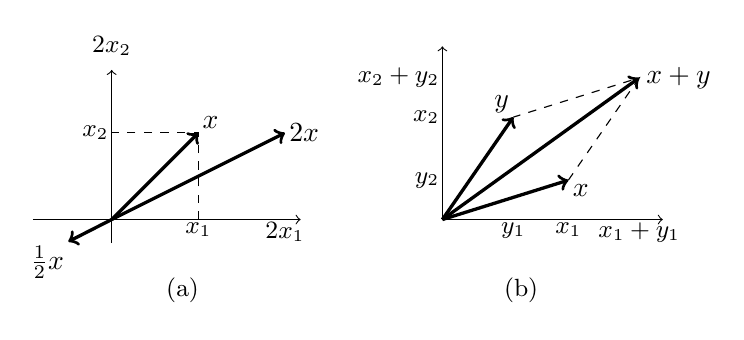
\begin{tikzpicture}[scale=1.0]
\begin{scope}[shift={(0,0)}]
\draw[->] (-1.0,0) -- (2.4,0);
\draw[->] (0,-0.3) -- (0,1.9);
\draw[dashed] (1.1,0) -- (1.1,1.1) -- (0,1.1);
\draw[very thick,->] (0,0) -- (1.1,1.1) node[above right,inner sep=1pt] {$\bm{x}$};
\draw[very thick,->] (0,0) -- (2.2,1.1) node[right,inner sep=1pt] {$2\bm{x}$};
\draw[very thick,->] (0,0) -- (-0.55,-0.28) node[below left,inner sep=1pt] {$\frac{1}{2}\bm{x}$};
\draw (0,1.1) node[left,inner sep=1pt] {\small $x_2$};
\draw (1.1,0) node[below,inner sep=1pt] {\small $x_1$};
\draw (2.2,0) node[below,inner sep=1pt] {\small $2x_1$};
\draw (0,2.2) node {\small $2x_2$};
\draw (0.9,-0.9) node {\small (a)};
\end{scope}
\begin{scope}[shift={(4.2,0)}]
\draw[->] (0,0) -- (2.8,0);
\draw[->] (0,0) -- (0,2.2);
\draw[very thick,->] (0,0) -- (1.6,0.5) node[below right,inner sep=1pt] {$\bm{x}$};
\draw[very thick,->] (0,0) -- (0.9,1.3) node[above left,inner sep=1pt] {$\bm{y}$};
\draw[dashed] (1.6,0.5) -- (2.5,1.8) -- (0.9,1.3);
\draw[very thick,->] (0,0) -- (2.5,1.8) node[right,inner sep=2pt] {$\bm{x}+\bm{y}$};
\draw (0,0.5) node[left,inner sep=1pt] {\small $y_2$};
\draw (0,1.3) node[left,inner sep=1pt] {\small $x_2$};
\draw (0,1.8) node[left,inner sep=1pt] {\small $x_2+y_2$};
\draw (1.6,0) node[below,inner sep=1pt] {\small $x_1$};
\draw (0.9,0) node[below,inner sep=1pt] {\small $y_1$};
\draw (2.5,0) node[below,inner sep=1pt] {\small $x_1+y_1$};
\draw (1.0,-0.9) node {\small (b)};
\end{scope}
\end{tikzpicture}
\phantomsection\label{fig:2.2}\mvcap{图 2.2\quad 标量乘法与向量加法}
\end{mvfigure}

\[
\bm{x}+\bm{y}=\begin{bmatrix}x_1\\x_2\\\vdots\\x_n\end{bmatrix}+\begin{bmatrix}y_1\\y_2\\\vdots\\y_n\end{bmatrix}=\begin{bmatrix}x_1+y_1\\x_2+y_2\\\vdots\\x_n+y_n\end{bmatrix}
\]

因此,$\bm{x}+\bm{y}$ 是一个向量,其第 $i$ 个元素为 $x_i+y_i$.

两个从坐标原点出发的向量之和,是以这两个向量为邻边所构成的平行四边形的对角
线,其几何解释见\hyperref[fig:2.2]{图 2.2}(b).

一个向量既有方向又有长度. 考虑 $n=2$ 维情形下的向量

\[
\bm{x}=\begin{bmatrix}x_1\\x_2\end{bmatrix}
\]

$\bm{x}$ 的长度记做 $L_x$,其定义为

\[
L_x=\sqrt{x_1^2+x_2^2}
\]

一个二维向量的长度在几何上可视做直角三角形斜边的长度,如\hyperref[fig:2.3]{图 2.3} 所示.

\begin{mvfigure}
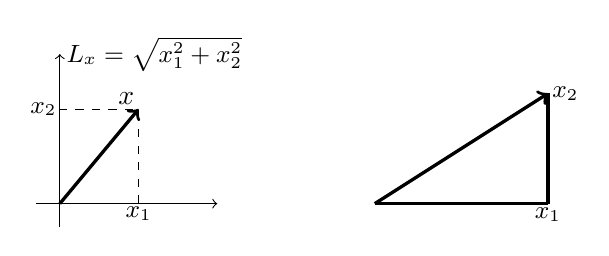
\begin{tikzpicture}[scale=1.0]
\begin{scope}[shift={(0,0)}]
\draw[->] (-0.3,0) -- (2.0,0);
\draw[->] (0,-0.3) -- (0,1.9);
\draw[dashed] (1.0,0) -- (1.0,1.2) -- (0,1.2);
\draw[very thick,->] (0,0) -- (1.0,1.2) node[above left,inner sep=1pt] {$\bm{x}$};
\draw (0,1.2) node[left,inner sep=1pt] {\small $x_2$};
\draw (1.0,0) node[below,inner sep=1pt] {\small $x_1$};
\draw (1.2,1.9) node {\small $L_x=\sqrt{x_1^2+x_2^2}$};
\end{scope}
\begin{scope}[shift={(4.0,0)}]
\draw[very thick] (0,0) -- (2.2,0) node[below,inner sep=1pt] {\small $x_1$};
\draw[very thick] (2.2,0) -- (2.2,1.4) node[right,inner sep=1pt] {\small $x_2$};
\draw[very thick,->] (0,0) -- (2.2,1.4);
\end{scope}
\end{tikzpicture}
\phantomsection\label{fig:2.3}\mvcap{图 2.3\quad $\bm{x}$ 的长度$=\sqrt{x_1^2+x_2^2}$}
\end{mvfigure}

有 $n$ 个分量的向量 $\bm{x}'=[x_1,x_2,\cdots,x_n]$ 的长度可用下式定义：

\phantomsection\label{eq:2-1}
\begin{equation}
L_x=\sqrt{x_1^2+x_2^2+\cdots+x_n^2} \tag{2-1}
\end{equation}

向量 $\bm{x}$ 乘以标量 $c$ 之后其长度发生改变,由\hyperref[eq:2-1]{式(2-1)}可知：

\begin{align*}
L_{cx}&=\sqrt{c^2x_1^2+c^2x_2^2+\cdots+c^2x_n^2}\\
&=|c|\sqrt{x_1^2+x_2^2+\cdots+x_n^2}=|c|\,L_x
\end{align*}

若 $c>0$,则用 $c$ 乘向量 $\bm{x}$ 不改变 $\bm{x}$ 的方向. 然而用负数 $c$ 乘 $\bm{x}$ 则产生一个与 $\bm{x}$ 方向相反的
向量. 从

\phantomsection\label{eq:2-2}
\begin{equation}
L_{cx}=|c|\,L_x \tag{2-2}
\end{equation}

%% ===== pg-053 =====

% ---- pg-053 （书页 41） ----
看得很清楚:若 $|c|>1$,则 $\bm{x}$ 延长;若 $0<|c|<1$,则 $\bm{x}$ 缩短[回顾\hyperref[fig:2.2]{图 2.2}(a)].选取 $c = L_x^{-1}$,便得到长度为 1 且与 $\bm{x}$ 同方向的单位向量 $L_x^{-1}\bm{x}$.

第二个几何概念是角.考虑平面内两个向量以及它们之间的夹角 $\theta$,如\hyperref[fig:2.4]{图 2.4} 所示.由图可见,$\theta$ 可表示成这两个向量分别同第一坐标轴的夹角 $\theta_1$ 和 $\theta_2$ 之差.因为,根据定义,

\[
\cos(\theta_1) = \frac{x_1}{L_x} \qquad \cos(\theta_2) = \frac{y_1}{L_y}
\]
\[
\sin(\theta_1) = \frac{x_2}{L_x} \qquad \sin(\theta_2) = \frac{y_2}{L_y}
\]

因而

\[
\cos(\theta) = \cos(\theta_2 - \theta_1) = \cos(\theta_2)\cos(\theta_1) + \sin(\theta_2)\sin(\theta_1)
\]

两个向量 $\bm{x}' = [x_1, x_2]$ 和 $\bm{y}' = [y_1, y_2]$ 之间的夹角 $\theta$ 由下式确定:

\phantomsection\label{eq:2-3}
\begin{equation}
\cos(\theta) = \cos(\theta_2 - \theta_1) = \left(\frac{y_1}{L_y}\right)\left(\frac{x_1}{L_x}\right) + \left(\frac{y_2}{L_y}\right)\left(\frac{x_2}{L_x}\right) = \frac{x_1y_1 + x_2y_2}{L_xL_y} \tag{2-3}
\end{equation}

我们发现引进两个向量的内积是方便的.对于 $n=2$ 维情形,$\bm{x}$ 和 $\bm{y}$ 的内积为

\[
\bm{x}'\bm{y} = x_1y_1 + x_2y_2
\]

根据这个定义和\hyperref[eq:2-3]{式(2-3)},有

\[
L_x = \sqrt{\bm{x}'\bm{x}} \qquad \cos(\theta) = \frac{\bm{x}'\bm{y}}{L_xL_y} = \frac{\bm{x}'\bm{y}}{\sqrt{\bm{x}'\bm{x}}\sqrt{\bm{y}'\bm{y}}}
\]

因为 $\cos(90^\circ) = \cos(270^\circ) = 0$,且仅当 $\bm{x}'\bm{y} = 0$ 时 $\cos(\theta) = 0$,所以当 $\bm{x}'\bm{y} = 0$ 时 $\bm{x}$ 与 $\bm{y}$ 互相垂直.

对任意维数 $n$,定义 $\bm{x}$ 与 $\bm{y}$ 的内积如下:

\phantomsection\label{eq:2-4}
\begin{equation}
\bm{x}'\bm{y} = x_1y_1 + x_2y_2 + \cdots + x_ny_n \tag{2-4}
\end{equation}

内积用 $\bm{x}'\bm{y}$ 或 $\bm{y}'\bm{x}$ 表示.

利用内积,就能将 $n$ 个分量的向量的长度和夹角自然地推广为

\phantomsection\label{eq:2-5}
\begin{equation}
L_x = \bm{x} \text{ 的长度} = \sqrt{\bm{x}'\bm{x}} \tag{2-5}
\end{equation}

\phantomsection\label{eq:2-6}
\begin{equation}
\cos(\theta) = \frac{\bm{x}'\bm{y}}{L_xL_y} = \frac{\bm{x}'\bm{y}}{\sqrt{\bm{x}'\bm{x}}\sqrt{\bm{y}'\bm{y}}} \tag{2-6}
\end{equation}

还是因为仅当 $\bm{x}'\bm{y} = 0$ 时 $\cos(\theta) = 0$,所以我们说,当 $\bm{x}'\bm{y} = 0$ 时 $\bm{x}$ 与 $\bm{y}$ 互相垂直.

\mvbold{例 2.1} （计算向量的长度和它们之间的夹角）

给定向量 $\bm{x}' = [1, 3, 2]$ 和 $\bm{y}' = [-2, 1, -1]$,求 $3\bm{x}$ 和 $\bm{x} + \bm{y}$.然后确定 $\bm{x}$ 的长度,$\bm{y}$ 的长度以及 $\bm{x}$ 与 $\bm{y}$ 之间的夹角.最后检验 $3\bm{x}$ 的长度是 $\bm{x}$ 长度的 3 倍.

首先,

\[
3\bm{x} = 3\begin{bmatrix} 1 \\ 3 \\ 2 \end{bmatrix} = \begin{bmatrix} 3 \\ 9 \\ 6 \end{bmatrix}
\]

\[
\bm{x} + \bm{y} = \begin{bmatrix} 1 \\ 3 \\ 2 \end{bmatrix} + \begin{bmatrix} -2 \\ 1 \\ -1 \end{bmatrix} = \begin{bmatrix} 1 - 2 \\ 3 + 1 \\ 2 - 1 \end{bmatrix} = \begin{bmatrix} -1 \\ 4 \\ 1 \end{bmatrix}
\]

\begin{mvfigure}
\begin{tikzpicture}[scale=1.1]
\draw[->] (0,0) -- (3.6,0) node[right] {$x$};
\draw[->] (0,0) -- (0,2.6) node[above] {$y$};
\draw[->] (0,0) -- (2.6,1.5) node[right] {$\bm{y}$};
\draw[->] (0,0) -- (3.0,1.0) node[above right] {$\bm{x}$};
\draw (0.9,0) arc (0:22:0.9);
\draw (1.2,0) arc (0:30:1.2);
\node at (1.35,0.16) {$\theta_2$};
\node at (1.75,0.30) {$\theta$};
\node at (0.55,0.35) {$\theta_1$};
\node[left] at (0,2.0) {$y_2$};
\node[below] at (2.0,0) {$x_2$};
\node[below] at (0.95,0) {$y_1$};
\node[below] at (2.85,0) {$x_1$};
\draw[dashed] (0,1.5) -- (2.0,1.5);
\draw[dashed] (2.0,0) -- (2.0,1.5);
\draw[dashed] (0,1.0) -- (1.0,1.0);
\draw[dashed] (1.0,0) -- (1.0,1.0);
\node at (1.9,1.85) {$\cos(\theta) = \dfrac{x_1y_1 + x_2y_2}{L_xL_y}$};
\end{tikzpicture}
\phantomsection\label{fig:2.4}\mvcap{图 2.4\quad $\bm{x}' = [x_1, x_2]$ 与 $\bm{y}' = [y_1, y_2]$ 之间的夹角 $\theta$}
\end{mvfigure}

%% ===== pg-054 =====

% ---- pg-054 （书页 42） ----
其次,由 $\bm{x}'\bm{x} = 1^2 + 3^2 + 2^2 = 14$，$\bm{y}'\bm{y} = (-2)^2 + 1^2 + (-1)^2 = 6$,以及 $\bm{x}'\bm{y} = 1 \times (-2) + 3 \times 1 + 2 \times (-1) = -1$,有

\[
L_x = \sqrt{\bm{x}'\bm{x}} = \sqrt{14} = 3.742 \qquad L_y = \sqrt{\bm{y}'\bm{y}} = \sqrt{6} = 2.449
\]

和

\[
\cos(\theta) = \frac{\bm{x}'\bm{y}}{L_xL_y} = \frac{-1}{3.742 \times 2.449} = -0.109
\]

于是 $\theta = 96.3^\circ$.最后

\[
L_{3x} = \sqrt{3^2 + 9^2 + 6^2} = \sqrt{126}, \quad 3L_x = 3\sqrt{14} = \sqrt{126}
\]

可见 $L_{3x} = 3L_x$.

一对同维向量 $\bm{x}$ 和 $\bm{y}$,如果存在两个不全为零的常数 $c_1$ 和 $c_2$,满足

\phantomsection\label{eq:2-7}
\begin{equation}
c_1\bm{x} + c_2\bm{y} = \bm{0} \tag{2-7}
\end{equation}

就说这对向量线性相关.一组向量 $\bm{x}_1, \bm{x}_2, \cdots, \bm{x}_k$,如果存在不全为零的常数 $c_1, c_2, \cdots, c_k$,使得

\[
c_1\bm{x}_1 + c_2\bm{x}_2 + \cdots + c_k\bm{x}_k = \bm{0}
\]

就说这组向量线性相关.

线性相关意味着:这组向量中至少有一个向量能写成其余向量的线性组合.如果几个同维向量并不线性相关,就说它们线性无关.

\mvbold{例 2.2} （识别线性无关向量）

考虑向量组

\[
\bm{x}_1 = \begin{bmatrix} 1 \\ 2 \\ 1 \end{bmatrix} \qquad \bm{x}_2 = \begin{bmatrix} 1 \\ 0 \\ -1 \end{bmatrix} \qquad \bm{x}_3 = \begin{bmatrix} 1 \\ -2 \\ 1 \end{bmatrix}
\]

令

\[
c_1\bm{x}_1 + c_2\bm{x}_2 + c_3\bm{x}_3 = \bm{0}
\]

可推出

\[
c_1 + c_2 + c_3 = 0
\]
\[
2c_1 \qquad - 2c_3 = 0
\]
\[
c_1 - c_2 + c_3 = 0
\]

有唯一解 $c_1 = c_2 = c_3 = 0$.由于找不到不全为零的常数 $c_1$,$c_2$ 和 $c_3$,使得 $c_1\bm{x}_1 + c_2\bm{x}_2 + c_3\bm{x}_3 = \bm{0}$,因而向量 $\bm{x}_1$,$\bm{x}_2$ 和 $\bm{x}_3$ 线性无关.

向量 $\bm{x}$ 在向量 $\bm{y}$ 上的投影(或影子)为

\phantomsection\label{eq:2-8}
\begin{equation}
\bm{x} \text{ 在 } \bm{y} \text{ 上的投影} = \left(\frac{\bm{x}'\bm{y}}{\bm{y}'\bm{y}}\right)\bm{y} = \left(\frac{\bm{x}'\bm{y}}{L_y}\right)\frac{1}{L_y}\bm{y} \tag{2-8}
\end{equation}

其中向量 $L_y^{-1}\bm{y}$ 的长度为 1.投影的长度为

\phantomsection\label{eq:2-9}
\begin{equation}
\text{投影的长度} = \left| \frac{\bm{x}'\bm{y}}{L_y} \right| = L_x\left| \frac{\bm{x}'\bm{y}}{L_xL_y} \right| = L_x| \cos(\theta) | \tag{2-9}
\end{equation}

其中 $\theta$ 是 $\bm{x}$ 与 $\bm{y}$ 间的夹角(见\hyperref[fig:2.5]{图 2.5}).

\begin{mvfigure}
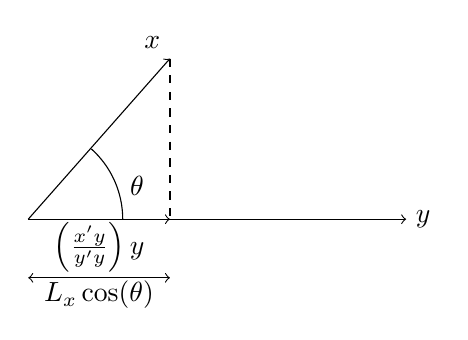
\begin{tikzpicture}[scale=1.2]
\draw[->] (0,0) -- (4.0,0) node[right] {$\bm{y}$};
\draw[->] (0,0) -- (1.5,1.7) node[above left] {$\bm{x}$};
\draw[dashed] (1.5,1.7) -- (1.5,0);
\draw[->] (0,0) -- (1.5,0);
\node[below,inner sep=1pt] at (0.75,0) {$\left(\frac{\bm{x}'\bm{y}}{\bm{y}'\bm{y}}\right)\bm{y}$};
\draw (1.0,0) arc (0:48:1.0);
\node at (1.15,0.35) {$\theta$};
\draw[<->] (0,-0.62) -- (1.5,-0.62);
\node[below,inner sep=1pt] at (0.75,-0.62) {$L_x\cos(\theta)$};
\end{tikzpicture}
\phantomsection\label{fig:2.5}\mvcap{图 2.5\quad $\bm{x}$ 在 $\bm{y}$ 上的投影}
\end{mvfigure}

\mvsub{矩阵}

由实数组成的任何矩形数表称为矩阵.我们将一个 $n$ 行 $p$ 列的任意数表示成

%% ===== pg-055 =====

% ---- pg-055 （书页 43） ----

\[
\underset{(n\times p)}{\bm{A}} =
\begin{bmatrix}
a_{11} & a_{12} & \cdots & a_{1p} \\
a_{21} & a_{22} & \cdots & a_{2p} \\
\vdots & \vdots & \ddots & \vdots \\
a_{n1} & a_{n2} & \cdots & a_{np}
\end{bmatrix}
\]

刚才引进的许多向量概念可直接推广到矩阵.

矩阵的转置运算 $\bm{A}'$ 把列变成行.这样变换后,$\bm{A}$ 的第一列成为 $\bm{A}'$ 的第一行,第二列成为第二行,依此类推.

\mvbold{例 2.3}\quad (矩阵的转置)

如果
\[
\underset{(2\times 3)}{\bm{A}} =
\begin{bmatrix}
3 & -1 & 2 \\
1 & 5 & 4
\end{bmatrix}
\]
则
\[
\underset{(3\times 2)}{\bm{A}'} =
\begin{bmatrix}
3 & 1 \\
-1 & 5 \\
2 & 4
\end{bmatrix}
\quad\blacksquare
\]

矩阵也可乘以常数 $c$.乘积 $c\bm{A}$ 也是矩阵,其元素为矩阵 $\bm{A}$ 的每个元素乘 $c$ 后所得之结果,即
\[
\underset{(n\times p)}{c\bm{A}} =
\begin{bmatrix}
ca_{11} & ca_{12} & \cdots & ca_{1p} \\
ca_{21} & ca_{22} & \cdots & ca_{2p} \\
\vdots & \vdots & \ddots & \vdots \\
ca_{n1} & ca_{n2} & \cdots & ca_{np}
\end{bmatrix}
\]

相同维数的两个矩阵 $\bm{A}$ 和 $\bm{B}$ 可以相加.矩阵和 $\bm{A}+\bm{B}$ 的第 $(i,j)$ 个元素为 $a_{ij}+b_{ij}$.

\mvbold{例 2.4}\quad (两矩阵之和及矩阵与常数之积)

如果
\[
\underset{(2\times 3)}{\bm{A}} =
\begin{bmatrix}
0 & 3 & 1 \\
1 & -1 & 1
\end{bmatrix}
\quad\text{和}\quad
\underset{(2\times 3)}{\bm{B}} =
\begin{bmatrix}
1 & -2 & -3 \\
2 & 5 & 1
\end{bmatrix}
\]
则
\[
\underset{(2\times 3)}{4\bm{A}} =
\begin{bmatrix}
0 & 12 & 4 \\
4 & -4 & 4
\end{bmatrix}
\quad\text{和}
\]
\[
\underset{(2\times 3)}{\bm{A}} + \underset{(2\times 3)}{\bm{B}} =
\begin{bmatrix}
0+1 & 3-2 & 1-3 \\
1+2 & -1+5 & 1+1
\end{bmatrix}
=
\underset{(2\times 3)}{\begin{bmatrix}
1 & 1 & -2 \\
3 & 4 & 2
\end{bmatrix}}
\quad\blacksquare
\]

如果两个矩阵的维数符合下面的要求,也可定义两个矩阵的乘法: 当 $\bm{A}$ 为 $(n\times k)$ 时,$\bm{B}$ 为 $(k\times p)$ 矩阵.就是说,当 $\bm{A}$ 的行元素个数与 $\bm{B}$ 的列元素个数相同时,就可以构造矩阵的乘积 $\bm{A}\bm{B}$.新矩阵 $\bm{A}\bm{B}$ 的元素由 $\bm{A}$ 的每一行与 $\bm{B}$ 的每一列的内积构成.

矩阵乘积 $\bm{A}\bm{B}$ 为
\[
\begin{gathered}
\underset{(n\times k)}{\bm{A}}\,\underset{(k\times p)}{\bm{B}} = (n\times p)\ \text{矩阵,其中第 } i \text{ 行第 } j \text{ 列元素是 } \bm{A} \text{ 的第 } i \text{ 行} \\
\text{与 } \bm{B} \text{ 的第 } j \text{ 列的内积}
\end{gathered}
\]

或
\phantomsection\label{eq:2-10}
\begin{equation}
\bm{A}\bm{B} \text{ 的第 } (i,j) \text{ 元素} = a_{i1}b_{1j} + a_{i2}b_{2j} + \cdots + a_{ik}b_{kj} = \sum_{l=1}^{k} a_{il}b_{lj} \tag{2-10}
\end{equation}

当 $k=4$ 时,矩阵 $\bm{A}\bm{B}$ 中的每一元素便是 4 项乘积之和.因此,%

%% ===== pg-056 =====

% ---- pg-056 （书页 44） ----

\[
\begin{gathered}
\underset{(n\times 4)}{\bm{A}}\ \underset{(4\times p)}{\bm{B}} =
\left[\begin{array}{cccc}
a_{11} & a_{12} & a_{13} & a_{14} \\
\vdots & \vdots & \vdots & \vdots \\
\cline{1-4}
a_{i1} & a_{i2} & a_{i3} & a_{i4} \\
\cline{1-4}
\vdots & \vdots & \vdots & \vdots \\
a_{n1} & a_{n2} & a_{n3} & a_{n4}
\end{array}\right]
\left[\begin{array}{cc|c|cc}
b_{11} & \cdots & b_{1j} & \cdots & b_{1p} \\
b_{21} & \cdots & b_{2j} & \cdots & b_{2p} \\
b_{31} & \cdots & b_{3j} & \cdots & b_{3p} \\
b_{41} & \cdots & b_{4j} & \cdots & b_{4p}
\end{array}\right] \\[4pt]
\begin{array}{c}
\text{列} \\
j \\
\vdots \\
= \text{行 } i\left[\cdots\left(a_{i1}b_{1j} + a_{i2}b_{2j} + a_{i3}b_{3j} + a_{i4}b_{4j}\right)\cdots\right] \\
\vdots
\end{array}
\end{gathered}
\]

\mvbold{例 2.5}\quad (矩阵乘法)

如果
\[
\bm{A} =
\begin{bmatrix}
3 & -1 & 2 \\
1 & 5 & 4
\end{bmatrix},
\quad
\bm{B} =
\begin{bmatrix}
-2 \\
7 \\
9
\end{bmatrix}
\quad\text{和}\quad
\bm{C} =
\begin{bmatrix}
2 & 0 \\
1 & -1
\end{bmatrix}
\]
则
\[
\underset{(2\times 3)}{\bm{A}}\,\underset{(3\times 1)}{\bm{B}} =
\begin{bmatrix}
3 & -1 & 2 \\
1 & 5 & 4
\end{bmatrix}
\begin{bmatrix}
-2 \\
7 \\
9
\end{bmatrix}
=
\begin{bmatrix}
3\times(-2)+(-1)\times 7+2\times 9 \\
1\times(-2)+5\times 7 \quad +4\times 9
\end{bmatrix}
=
\underset{(2\times 1)}{\begin{bmatrix}
5 \\
69
\end{bmatrix}}
\]
和
\[
\underset{(2\times 2)}{\bm{C}}\,\underset{(2\times 3)}{\bm{A}} =
\begin{bmatrix}
2 & 0 \\
1 & -1
\end{bmatrix}
\begin{bmatrix}
3 & -1 & 2 \\
1 & 5 & 4
\end{bmatrix}
\]
\[
=
\begin{bmatrix}
2\times 3+0\times 1 & 2\times(-1)+0\times 5 & 2\times 2+0\times 4 \\
1\times 3-1\times 1 & 1\times(-1)-1\times 5 & 1\times 2-1\times 4
\end{bmatrix}
=
\underset{(2\times 3)}{\begin{bmatrix}
6 & -2 & 4 \\
2 & -6 & -2
\end{bmatrix}}
\]

当矩阵 $\bm{B}$ 由一列组成时,通常采用小写的向量符号 $\bm{b}$.\hfill$\blacksquare$

\mvbold{例 2.6}\quad (某些典型的乘积以及它们的维数)

设
\[
\bm{A} =
\begin{bmatrix}
1 & -2 & 3 \\
2 & 4 & -1
\end{bmatrix}
\qquad
\bm{b} =
\begin{bmatrix}
7 \\
-3 \\
6
\end{bmatrix}
\qquad
\bm{c} =
\begin{bmatrix}
5 \\
8 \\
-4
\end{bmatrix}
\qquad
\bm{d} =
\begin{bmatrix}
2 \\
9
\end{bmatrix}
\]

此时 $\bm{A}\bm{b},\bm{b}\bm{c}',\bm{b}'\bm{c}$ 和 $\bm{d}'\bm{A}\bm{b}$ 为典型的乘积.

\[
\bm{A}\bm{b} =
\begin{bmatrix}
1 & -2 & 3 \\
2 & 4 & -1
\end{bmatrix}
\begin{bmatrix}
7 \\
-3 \\
6
\end{bmatrix}
=
\begin{bmatrix}
31 \\
-4
\end{bmatrix}
\]

乘积 $\bm{A}\bm{b}$ 是一个向量,其维数等于 $\bm{A}$ 的行数.

\[
\bm{b}'\bm{c} =
\begin{bmatrix}
7 & -3 & 6
\end{bmatrix}
\begin{bmatrix}
5 \\
8 \\
-4
\end{bmatrix}
=
\begin{bmatrix}
-13
\end{bmatrix}
\]

%% ===== pg-057 =====

% ---- pg-057 （书页 45） ----

乘积 $\bm{b}'\bm{c}$ 是一个 $1\times 1$ 向量或一个数,在这里等于 $-13$.
\[
\bm{b}\bm{c}' =
\begin{bmatrix}
7 \\
-3 \\
6
\end{bmatrix}
\begin{bmatrix}
5 & 8 & -4
\end{bmatrix}
=
\begin{bmatrix}
35 & 56 & -28 \\
-15 & -24 & 12 \\
30 & 48 & -24
\end{bmatrix}
\]

乘积 $\bm{b}\bm{c}'$ 是一矩阵,其行数等于 $\bm{b}$ 的维数,列数等于 $\bm{c}$ 的维数.这个积与 $\bm{b}'\bm{c}$ 不同,$\bm{b}'\bm{c}$ 是一个数.

\[
\bm{d}'\bm{A}\bm{b} =
\begin{bmatrix}
2 & 9
\end{bmatrix}
\begin{bmatrix}
1 & -2 & 3 \\
2 & 4 & -1
\end{bmatrix}
\begin{bmatrix}
7 \\
-3 \\
6
\end{bmatrix}
=
\begin{bmatrix}
26
\end{bmatrix}
\]

乘积 $\bm{d}'\bm{A}\bm{b}$ 是一个 $1\times 1$ 向量或一个数,在这里等于 26.\hfill$\blacksquare$

方阵在统计方法的开发中将具有特殊的重要性.对一个方阵,如果 $\bm{A}=\bm{A}'$ 或对所有 $i$ 和 $j$,$a_{ij}=a_{ji}$,则称此方阵为对称阵.

\mvbold{例 2.7}\quad (对称阵)

矩阵
\[
\begin{bmatrix}
3 & 5 \\
5 & -2
\end{bmatrix}
\]
是对称阵; 矩阵
\[
\begin{bmatrix}
3 & 6 \\
4 & -2
\end{bmatrix}
\]
则不是对称阵.\hfill$\blacksquare$

当两个方阵 $\bm{A}$ 和 $\bm{B}$ 维数相同时,两个乘积 $\bm{A}\bm{B}$ 和 $\bm{B}\bm{A}$ 均有定义,尽管它们未必相等(见补充 2A).若以 $\bm{I}$ 表示主对角线上元素均为 1,其余元素均为 0 的方阵,则按照矩阵乘法的定义,$\bm{A}\bm{I}$ 的第 $(i,j)$ 个元素为 $a_{i1}\times 0+\cdots+a_{i,i-1}\times 0+a_{ii}\times 1+a_{i,i+1}\times 0+\cdots+a_{ik}\times 0=a_{ij}$,于是 $\bm{A}\bm{I}=\bm{A}$.类似有 $\bm{I}\bm{A}=\bm{A}$.因此,对任何 $\bm{A}$ 有
\phantomsection\label{eq:2-11}
\begin{equation}
\underset{(k\times k)}{\bm{I}}\,\underset{(k\times k)}{\bm{A}} = \underset{(k\times k)}{\bm{A}}\,\underset{(k\times k)}{\bm{I}} = \underset{(k\times k)}{\bm{A}} \tag{2-11}
\end{equation}

矩阵 $\bm{I}$ 就像数字 1 在普通乘法中所起的作用一样 $(1\cdot a=a\cdot 1=a)$,因此称为单位矩阵.

如果 $a\neq 0$,就存在一个倒数 $a^{-1}$,能使 $a^{-1}a=aa^{-1}=1$,这个基本的数量关系在矩阵代数中有如下推广: 如果存在矩阵 $\bm{B}$,使得
\[
\underset{(k\times k)}{\bm{B}}\,\underset{(k\times k)}{\bm{A}} = \underset{(k\times k)}{\bm{A}}\,\underset{(k\times k)}{\bm{B}} = \underset{(k\times k)}{\bm{I}}
\]
则称 $\bm{B}$ 为 $\bm{A}$ 的逆矩阵,并记作 $\bm{A}^{-1}$.

存在逆矩阵的条件是: $\bm{A}$ 的 $k$ 个列 $\bm{a}_1,\bm{a}_2,\cdots,\bm{a}_k$ 线性无关.就是说,$\bm{A}^{-1}$ 的存在等价于
\phantomsection\label{eq:2-12}
\begin{equation}
c_1\bm{a}_1 + c_2\bm{a}_2 + \cdots + c_k\bm{a}_k = \bm{0} \quad\text{仅当}\quad c_1 = \cdots = c_k = 0 \text{ 时} \tag{2-12}
\end{equation}
(见补充 2A 中结论 2A.9.)

\mvbold{例 2.8}\quad (逆矩阵的存在性)

对于
\[
\underset{(2\times 2)}{\bm{A}} =
\begin{bmatrix}
3 & 2 \\
4 & 1
\end{bmatrix}
\]
可以验证
\[
\begin{bmatrix}
-0.2 & 0.4 \\
0.8 & -0.6
\end{bmatrix}
\begin{bmatrix}
3 & 2 \\
4 & 1
\end{bmatrix}
=
\begin{bmatrix}
(-0.2)\times 3 + \quad 0.4\times 4 & (-2)\times 2 + \quad 0.4\times 1 \\
0.8\times 3+(-0.6)\times 4 & 0.8\times 2+(-0.6)\times 1
\end{bmatrix}
\]

%% ===== pg-058 =====

% ---- pg-058 （书页 46） ----
\[
= \begin{bmatrix} 1 & 0 \\ 0 & 1 \end{bmatrix}
\]

于是

\[
\begin{bmatrix} -0.2 & 0.4 \\ 0.8 & -0.6 \end{bmatrix}
\]

便是 $\bm{A}^{-1}$.注意到

\[
c_1\begin{bmatrix} 3 \\ 4 \end{bmatrix} + c_2\begin{bmatrix} 2 \\ 2 \end{bmatrix} = \begin{bmatrix} 0 \\ 0 \end{bmatrix}
\]

意味着 $c_1 = c_2 = 0$,所以 $\bm{A}$ 的各列线性无关.这证实了\hyperref[eq:2-12]{式(2-12)}中所说的条件.

当逆矩阵存在时,其计算方法见补充 2A.这些冗长的程式化计算,通常由计算机完成,尤其当维数大于 3 时更是这样.即使如此,还是必须预先警告:如果对某些常数 $c_1$, $c_2, \cdots, c_k$ 来说\hyperref[eq:2-12]{式(2-12)}中的列和接近于 $\bm{0}$,由于舍入误差极大,计算机会产生错误的逆.因此当 $\bm{A}^{-1}$ 由一个计算机软件包所产生时,最好用乘积 $\bm{A}\bm{A}^{-1}$ 和 $\bm{A}^{-1}\bm{A}$ 是否等于 $\bm{I}$ 作一下检验(见练习 2.10).

有逆的对角阵很容易计算.例如,如果所有 $a_{ii} \neq 0$,则

\[
\begin{bmatrix}
a_{11} & 0 & 0 & 0 & 0 \\
0 & a_{22} & 0 & 0 & 0 \\
0 & 0 & a_{33} & 0 & 0 \\
0 & 0 & 0 & a_{44} & 0 \\
0 & 0 & 0 & 0 & a_{55}
\end{bmatrix}
\qquad \text{有逆矩阵} \qquad
\begin{bmatrix}
\dfrac{1}{a_{11}} & 0 & 0 & 0 & 0 \\[2mm]
0 & \dfrac{1}{a_{22}} & 0 & 0 & 0 \\[2mm]
0 & 0 & \dfrac{1}{a_{33}} & 0 & 0 \\[2mm]
0 & 0 & 0 & \dfrac{1}{a_{44}} & 0 \\[2mm]
0 & 0 & 0 & 0 & \dfrac{1}{a_{55}}
\end{bmatrix}
\]

我们要熟悉的另一类特殊方阵是正交矩阵,其特征为

\phantomsection\label{eq:2-13}
\begin{equation}
\bm{Q}\bm{Q}' = \bm{Q}'\bm{Q} = \bm{I} \quad \text{或} \quad \bm{Q}' = \bm{Q}^{-1} \tag{2-13}
\end{equation}

正交矩阵的名称来自其性质,即如果 $\bm{Q}$ 的第 $i$ 行是 $\bm{q}_i'$,则 $\bm{Q}\bm{Q}' = \bm{I}$ 意味着 $\bm{q}_i'\bm{q}_i = 1$ 和 $\bm{q}_i'\bm{q}_j = 0$ $(i \neq j)$,因此,每一行均具有单位长度且行与行之间互相垂直(正交).根据条件 $\bm{Q}'\bm{Q} = \bm{I}$ 列也有同样的性质.

在结束对矩阵代数原理的简单介绍时,我们引入一个多元统计分析的基本概念.一个方阵 $\bm{A}$,如果有

\phantomsection\label{eq:2-14}
\begin{equation}
\bm{A}\bm{x} = \lambda\bm{x} \tag{2-14}
\end{equation}

则说方阵 $\bm{A}$ 具有特征值 $\lambda$ 和对应的特征向量 $\bm{x} \neq \bm{0}$.通常,将 $\bm{x}$ 标准化使其具有单位长度,即 $1 = \bm{x}'\bm{x}$.为方便起见,在下文中用 $\bm{e}$ 表示标准化的特征向量.我们省去详细的推导过程(见[1]),给出如下的基本结论:

\begin{mvbox}
设 $\bm{A}$ 是 $k \times k$ 对称方阵,则 $\bm{A}$ 有 $k$ 对特征值和特征向量,即

\phantomsection\label{eq:2-15}
\begin{equation}
\lambda_1, \bm{e}_1, \qquad \lambda_2, \bm{e}_2, \qquad \cdots \qquad \lambda_k, \bm{e}_k \tag{2-15}
\end{equation}

可以选择特征向量,使其满足 $1 = \bm{e}_i'\bm{e}_i = \cdots = \bm{e}_k'\bm{e}_k$ 且互相垂直.除非两个或多个特征值是相等的,对应特征值的特征向量是唯一的.
\end{mvbox}

%% ===== pg-059 =====

% ---- pg-059 （书页 47） ----
\mvbold{例 2.9} （检验特征值和特征向量）

设

\[
\bm{A} = \begin{bmatrix} 1 & -5 \\ -5 & 1 \end{bmatrix}
\]

则,因为

\[
\begin{bmatrix} 1 & -5 \\ -5 & 1 \end{bmatrix}\begin{bmatrix} \dfrac{1}{\sqrt{2}} \\[2mm] -\dfrac{1}{\sqrt{2}} \end{bmatrix} = 6\begin{bmatrix} \dfrac{1}{\sqrt{2}} \\[2mm] -\dfrac{1}{\sqrt{2}} \end{bmatrix}
\]

所以 $\lambda_1 = 6$ 是一个特征值,且

\[
\bm{e}_1 = \begin{bmatrix} \dfrac{1}{\sqrt{2}} \\[2mm] -\dfrac{1}{\sqrt{2}} \end{bmatrix}
\]

是 $\lambda_1$ 对应的标准化特征向量.可以证明还有一对特征值-特征向量是 $\lambda_2 = -4$, $\bm{e}_2' = [1/\sqrt{2}, 1/\sqrt{2}]$.

在补充 2A 中,给出了计算 $\lambda$ 和 $\bm{e}$ 的一种方法.当方阵维数大于 2 或 3 时,通常要依靠计算机计算.可以做几个实例计算来理解该方法,这是有好处的.

\section{正定矩阵}  % 原书 2.3
\phantomsection\label{sec:2.3}

研究多元数据中的变量及其相互关系时,通常以距离和数据多元正态分布假设为基础.距离的平方(见第 1 章)和多元正态密度可以用称为二次型(见第 4 章)的矩阵乘积来表示.因此,毫不奇怪,在多元分析中二次型起着重要作用.在本节中,我们考虑总是非负的二次型及相关联的正定矩阵.

涉及二次型和对称矩阵的许多结论,在多数情况下,可直接由对称阵的称为谱分解的展开式得出.一个 $k \times k$ 对称阵 $\bm{A}$ 的谱分解由\hyperref[eq:2-16]{式(2-16)}给出.\footnote{式(2-16)的证明超出本书范围.有兴趣的读者可以在第 8 章的文献[6]找到证明方法.}

\phantomsection\label{eq:2-16}
\begin{equation}
\begin{array}{llclclclclcl}
\bm{A} & = & \lambda_1 & \bm{e}_1 & \bm{e}_1' & +\ \lambda_2 & \bm{e}_2 & \bm{e}_2' & +\ \cdots & +\ \lambda_k & \bm{e}_k & \bm{e}_k' \\
(k \times k) & & & (k \times 1) & (1 \times k) & & (k \times 1) & (1 \times k) & & & (k \times 1) & (1 \times k)
\end{array} \tag{2-16}
\end{equation}

其中 $\lambda_1, \lambda_2, \cdots, \lambda_k$ 是 $\bm{A}$ 的特征值,$\bm{e}_1, \bm{e}_2, \cdots, \bm{e}_k$ 是相对应的标准化特征向量(参考补充 2A 中 2A.14 结论).因此有 $\bm{e}_i'\bm{e}_i = 1, i = 1, 2, \cdots, k$,且对 $i \neq j$, $\bm{e}_i'\bm{e}_j = 0$.

\mvbold{例 2.10} （矩阵的谱分解）

考虑对称矩阵

\[
\bm{A} = \begin{bmatrix} 13 & -4 & 2 \\ -4 & 13 & -2 \\ 2 & -2 & 10 \end{bmatrix}
\]

从特征方程 $|\bm{A} - \lambda\bm{I}| = 0$ 得到的特征值是 $\lambda_1 = 9$, $\lambda_2 = 9$ 和 $\lambda_3 = 18$(定义 2A.30).对应的特征向量 $\bm{e}_1$, $\bm{e}_2$ 和 $\bm{e}_3$ 是方程 $\bm{A}\bm{e}_i = \lambda_i\bm{e}_i$ $(i = 1, 2, 3)$ 的(标准化)解.因此,由 $\bm{A}\bm{e}_1 = \lambda\bm{e}_1$ 有

%% ===== pg-060 =====

% ---- pg-060 （书页 48） ----
\[
\begin{bmatrix} 13 & -4 & 2 \\ -4 & 13 & -2 \\ 2 & -2 & 10 \end{bmatrix}\begin{bmatrix} e_{11} \\ e_{21} \\ e_{31} \end{bmatrix} = 9\begin{bmatrix} e_{11} \\ e_{21} \\ e_{31} \end{bmatrix}
\]

或

\[
13e_{11} - 4e_{21} + 2e_{31} = 9e_{11}
\]
\[
-4e_{11} + 13e_{21} - 2e_{31} = 9e_{21}
\]
\[
2e_{11} - 2e_{21} + 10e_{31} = 9e_{31}
\]

把等号右边的项移至左边得到三个含三个未知数的齐次方程,其中两个方程是重复的.选择其中的一个方程并任意设 $e_{11} = 1$ 及 $e_{31} = 1$,求得 $e_{21} = 0$.由于标准化特征向量各元素的平方和是 1,因此,标准化特征向量为

\[
\bm{e}_1' = \left[1/\sqrt{1^2 + 1^2 + 0^2},\, 1/\sqrt{1^2 + 1^2 + 0^2},\, 0/\sqrt{1^2 + 1^2 + 0^2}\right] = [1/\sqrt{2}, 1/\sqrt{2}, 0]
\]

可以证明 $\bm{e}_2' = [1/\sqrt{18}, -1/\sqrt{18}, -4/\sqrt{18}]$ 也是 $\lambda_1 = 9$ 的标准化特征向量, $\bm{e}_3' = [2/3, -2/3, 1/3]$ 是特征值 $\lambda_3 = 18$ 相应的标准化特征向量.而且,对 $i \neq j$, $\bm{e}_i'\bm{e}_j = 0$.

容易证明,$\bm{A}$ 的谱分解是

\[
\bm{A} = \lambda_1\bm{e}_1\bm{e}_1' + \lambda_2\bm{e}_2\bm{e}_2' + \lambda_3\bm{e}_3\bm{e}_3'
\]

或

\[
\begin{bmatrix} 13 & -4 & 2 \\ -4 & 13 & -2 \\ 2 & -2 & 10 \end{bmatrix} = 9\begin{bmatrix} \dfrac{1}{\sqrt{2}} \\[2mm] \dfrac{1}{\sqrt{2}} \\[2mm] 0 \end{bmatrix}\begin{bmatrix} \dfrac{1}{\sqrt{2}} & \dfrac{1}{\sqrt{2}} & 0 \end{bmatrix}
\]
\[
+ 9\begin{bmatrix} \dfrac{1}{\sqrt{18}} \\[2mm] -\dfrac{1}{\sqrt{18}} \\[2mm] -\dfrac{4}{\sqrt{18}} \end{bmatrix}\begin{bmatrix} \dfrac{1}{\sqrt{18}} & -\dfrac{1}{\sqrt{18}} & -\dfrac{4}{\sqrt{18}} \end{bmatrix} + 18\begin{bmatrix} \dfrac{2}{3} \\[2mm] -\dfrac{2}{3} \\[2mm] \dfrac{1}{3} \end{bmatrix}\begin{bmatrix} \dfrac{2}{3} & -\dfrac{2}{3} & \dfrac{1}{3} \end{bmatrix}
\]
\[
= 9\begin{bmatrix} \dfrac{1}{2} & \dfrac{1}{2} & 0 \\[2mm] \dfrac{1}{2} & \dfrac{1}{2} & 0 \\[2mm] 0 & 0 & 0 \end{bmatrix} + 9\begin{bmatrix} \dfrac{1}{18} & -\dfrac{1}{18} & -\dfrac{4}{18} \\[2mm] -\dfrac{1}{18} & \dfrac{1}{18} & \dfrac{4}{18} \\[2mm] -\dfrac{4}{18} & \dfrac{4}{18} & \dfrac{16}{18} \end{bmatrix}
\]
\[
+ 18\begin{bmatrix} \dfrac{4}{9} & -\dfrac{4}{9} & \dfrac{2}{9} \\[2mm] -\dfrac{4}{9} & \dfrac{4}{9} & -\dfrac{2}{9} \\[2mm] \dfrac{2}{9} & -\dfrac{2}{9} & \dfrac{1}{9} \end{bmatrix}
\]

谱分解是一种重要的分析工具,利用它可以顺利地论证某些统计学结论.首先,我们研究距离的矩阵解释.

%% ===== pg-061 =====

% ---- pg-061 （书页 49） ----

设 $k\times k$ 对称矩阵 $\bm{A}$ 对于一切 $\bm{x}'=[x_1,x_2,\cdots,x_k]$，满足

\phantomsection\label{eq:2-17}
\begin{equation}
0\leqslant \bm{x}'\bm{A}\bm{x} \tag{2-17}
\end{equation}

则称 $\bm{A}$ 是非负定的.若仅当向量 $\bm{x}'=[0,0,\cdots,0]$ 时，\hyperref[eq:2-17]{式(2-17)}中等号才成立，则称 $\bm{A}$ 是正定的.换言之，如果对一切 $\bm{x}\neq \bm{0}$ 的向量，有

\phantomsection\label{eq:2-18}
\begin{equation}
0<\bm{x}'\bm{A}\bm{x} \tag{2-18}
\end{equation}

则称 $\bm{A}$ 是正定的.因为 $\bm{x}'\bm{A}\bm{x}$ 中只含有平方项 $x_i^2$ 及乘积项 $x_ix_j$，故称为二次型.

\mvbold{例 2.11} \quad (正定矩阵和二次型)

证明以下二次型是正定的：

\[
3x_1^2+2x_2^2-2\sqrt{2}x_1x_2
\]

为了说明一般方法，首先写出二次型的矩阵表示形式

\[
[x_1 \quad x_2]
\begin{bmatrix}
3 & -\sqrt{2}\\
-\sqrt{2} & 2
\end{bmatrix}
\begin{bmatrix}
x_1\\
x_2
\end{bmatrix}
=\bm{x}'\bm{A}\bm{x}
\]

由定义 2A.30，$\bm{A}$ 的特征值是方程 $|\bm{A}-\lambda \bm{I}|=0$ 或 $(3-\lambda)(2-\lambda)-2=0$ 的解.求解得，$\lambda_1=4$，$\lambda_2=1$.利用\hyperref[eq:2-16]{式(2-16)}的谱分解，有

\[
\underset{(2\times2)}{\bm{A}}=\underset{(2\times1)}{\lambda_1\bm{e}_1}\underset{(1\times2)}{\bm{e}_1'}+\underset{(2\times1)}{\lambda_2\bm{e}_2}\underset{(1\times2)}{\bm{e}_2'}
\]
\[
=\underset{(2\times1)}{4\bm{e}_1}\underset{(1\times2)}{\bm{e}_1'}+\underset{(2\times1)}{\bm{e}_2}\underset{(1\times2)}{\bm{e}_2'}
\]

其中 $\bm{e}_1$ 和 $\bm{e}_2$ 是分别对应于特征值 $\lambda_1=4$ 和 $\lambda_2=1$ 的标准化的正交的特征向量.因为 $4$ 和 $1$ 是标量，用 $\bm{x}'$ 和 $\bm{x}$ 分别左乘和右乘 $\bm{A}$，其中 $\bm{x}'=[x_1,x_2]$ 是任一非零向量，得

\[
\underset{(1\times2)}{\bm{x}'}\underset{(2\times2)}{\bm{A}}\underset{(2\times1)}{\bm{x}}=\underset{(1\times2)}{4\bm{x}'}\underset{(2\times1)}{\bm{e}_1}\underset{(1\times2)}{\bm{e}_1'}\underset{(2\times1)}{\bm{x}}+\underset{(1\times2)}{\bm{x}'}\underset{(2\times1)}{\bm{e}_2}\underset{(1\times2)}{\bm{e}_2'}\underset{(2\times1)}{\bm{x}}
\]
\[
=4y_1^2+y_2^2\geqslant 0
\]

其中

\[
y_1=\bm{x}'\bm{e}_1=\bm{e}_1'\bm{x} \qquad \text{和} \qquad y_2=\bm{x}'\bm{e}_2=\bm{e}_2'\bm{x}
\]

这表明，$y_1$ 和 $y_2$ 不全为零，因此，$\bm{x}'\bm{A}\bm{x}=4y_1^2+y_2^2>0$，即 $\bm{A}$ 是正定的.

从 $y_1$ 和 $y_2$ 的定义，有

\[
\begin{bmatrix}
y_1\\
y_2
\end{bmatrix}
=
\begin{bmatrix}
\bm{e}_1'\\
\bm{e}_2'
\end{bmatrix}
\begin{bmatrix}
x_1\\
x_2
\end{bmatrix}
\]

或

\[
\underset{(2\times1)}{\bm{y}}=\underset{(2\times2)}{\bm{E}}\underset{(2\times1)}{\bm{x}}
\]

现在 $\bm{E}$ 是正交阵，因而有逆矩阵 $\bm{E}'$.于是，$\bm{x}=\bm{E}'\bm{y}$.$\bm{x}$ 是非零向量，则 $\bm{0}\neq \bm{x}=\bm{E}'\bm{y}$ 意味着 $\bm{y}\neq \bm{0}$.

运用谱分解，很容易证明，当且仅当 $\bm{A}$ 的所有特征值均大于零时，$k\times k$ 对称阵 $\bm{A}$ 是正定矩阵(参考练习 2.17).当且仅当 $\bm{A}$ 的所有特征值大于或等于零时，$\bm{A}$ 是非负定阵.

现在假定向量 $\bm{x}$ 的 $p$ 个元素 $x_1,x_2,\cdots,x_p$ 被视为 $p$ 个随机变量 $X_1,X_2,\cdots,X_p$.正如第 1 章中指出的，可以把这些元素当做 $p$ 维空间中一个点的坐标；在这种情况下，点 $(x_1,x_2,\cdots,x_p)$ 到原点的“距离”应当利用单位标准偏差来表示.这样，我们可以解释观察结果中所固有的不确定性(变化性).具有相同的“不确定性”的点，可以看成与原点的距离相同.

利用第 1 章中介绍的距离公式[参见\hyperref[eq:1-22]{式(1-22)}]，假定对所有的 $[x_1,x_2,\cdots,x_p]\neq[0,0,\cdots,0]$，有(距离)$^2>0$，则到原点的距离满足一般公式

%% ===== pg-062 =====

% ---- pg-062 （书页 50） ----

\[
(\text{距离})^2=a_{11}x_1^2+a_{22}x_2^2+\cdots+a_{pp}x_p^2
\]
\[
\hspace{4em}+2(a_{12}x_1x_2+a_{13}x_1x_3+\cdots+a_{p-1,p}x_{p-1}x_p)
\]

令 $a_{ij}=a_{ji},i\neq j,i=1,2,\cdots,p,j=1,2,\cdots,p$，有

\[
0<(\text{距离})^2=[x_1,x_2,\cdots,x_p]
\begin{bmatrix}
a_{11} & a_{12} & \cdots & a_{1p}\\
a_{21} & a_{22} & \cdots & a_{2p}\\
\vdots & \vdots & & \vdots\\
a_{p1} & a_{p2} & \cdots & a_{pp}
\end{bmatrix}
\begin{bmatrix}
x_1\\
x_2\\
\vdots\\
x_p
\end{bmatrix}
\]

或

\phantomsection\label{eq:2-19}
\begin{equation}
0<(\text{距离})^2=\bm{x}'\bm{A}\bm{x},\text{对 } \bm{x}\neq \bm{0} \tag{2-19}
\end{equation}

从\hyperref[eq:2-19]{式(2-19)}可见，$p\times p$ 对称阵 $\bm{A}$ 是正定的.总之，距离是由一正定二次型 $\bm{x}'\bm{A}\bm{x}$ 所确定的.反过来，一个正定二次型可以解释为一个距离平方.

\mvbold{评注} \quad 设点 $\bm{x}'=[x_1,x_2,\cdots,x_p]$ 到原点的距离平方由 $\bm{x}'\bm{A}\bm{x}$ 给出，其中 $\bm{A}$ 是 $p\times p$ 对称正定矩阵，则从 $\bm{x}$ 到任意一固定点 $\bm{\mu}'=[\mu_1,\mu_2,\cdots,\mu_p]$ 的距离平方由一般表达式 $(\bm{x}-\bm{\mu})'\bm{A}(\bm{x}-\bm{\mu})$ 给出.

用一个正定二次型的平方根表示距离，使我们给出一个基于矩阵 $\bm{A}$ 的特征值和特征向量的几何解释.例如，设 $p=2$，则到原点的距离为常数 $c$ 的点 $\bm{x}'=[x_1,x_2]$，满足

\[
\bm{x}'\bm{A}\bm{x}=a_{11}x_1^2+a_{22}x_2^2+2a_{12}x_1x_2=c^2
\]

如例 2.11 中，按照谱分解

\[
\bm{A}=\lambda_1\bm{e}_1\bm{e}_1'+\lambda_2\bm{e}_2\bm{e}_2' \qquad \text{所以} \qquad \bm{x}'\bm{A}\bm{x}=\lambda_1(\bm{x}'\bm{e}_1)^2+\lambda_2(\bm{x}'\bm{e}_2)^2
\]

现在，令 $y_1=\bm{x}'\bm{e}_1,y_2=\bm{x}'\bm{e}_2,c^2=\lambda_1y_1^2+\lambda_2y_2^2$ 是一个椭圆，因为当 $\bm{A}$ 为正定时 $\lambda_1,\lambda_2>0$(参见练习 2.17).易证 $\bm{x}=c\lambda_1^{-1/2}\bm{e}_1$ 满足 $\bm{x}'\bm{A}\bm{x}=\lambda_1(c\lambda_1^{-1/2}\bm{e}_1')^2=c^2$.同样地，$\bm{x}=c\lambda_2^{-1/2}\bm{e}_2$ 给出了沿 $\bm{e}_2$ 方向的适当的距离.因此，距离为 $c$ 的点落在椭圆上，它的轴由 $\bm{A}$ 的特征向量给出，其长度与特征值的平方根的倒数成比例，比例常数就是 $c$.其位置如\hyperref[fig:2.6]{图 2.6} 所示.

如果 $p>2$，到原点距离为常数 $c=\sqrt{\bm{x}'\bm{A}\bm{x}}$ 的点 $\bm{x}'=[x_1,x_2,\cdots,x_p]$ 落在超椭球 $c^2=\lambda_1(\bm{x}'\bm{e}_1)^2+\cdots+\lambda_p(\bm{x}'\bm{e}_p)^2$ 上，其轴由 $\bm{A}$ 的特征向量给出.沿 $\bm{e}_i$ 方向的半轴长等于 $c/\sqrt{\lambda_i},i=1,2,\cdots,p$，其中 $\lambda_1,\lambda_2,\cdots,\lambda_p$ 是 $\bm{A}$ 的特征值.

\begin{mvfigure}
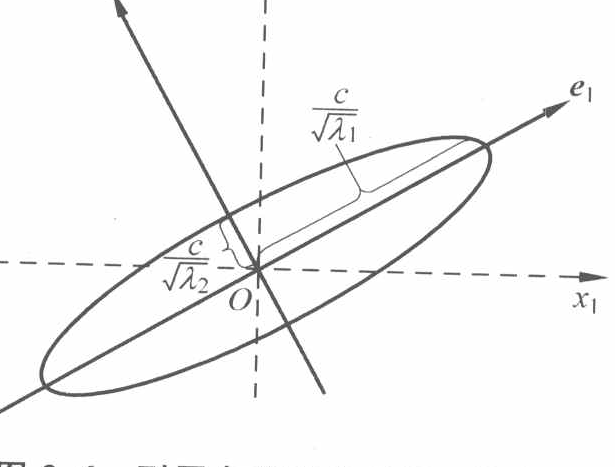
\includegraphics[width=52.1mm]{figs/fig_pg062_1.png}
\phantomsection\label{fig:2.6}\mvcap{图 2.6\quad 到原点距离为常数 $c$ 的点 $（p=2,1<\lambda_1<\lambda_2）$}
\end{mvfigure}

\section{平方根矩阵}  % 原书 2.4
\phantomsection\label{sec:2.4}

谱分解使我们可用方阵的特征值和特征向量来表示该方阵的逆，同时还带来一个有用的概念：平方根矩阵.

设 $\bm{A}$ 是 $k\times k$ 正定矩阵，有谱分解 $\bm{A}=\sum\limits_{i=1}^{k}\lambda_i\bm{e}_i\bm{e}_i'$.设标准化特征向量是另一矩阵的列向量 $\bm{P}=[\bm{e}_1,\bm{e}_2,\cdots,\bm{e}_k]$.于是有

\phantomsection\label{eq:2-20}
\begin{equation}
\underset{(k\times k)}{\bm{A}}=\sum_{i=1}^{k}\underset{(k\times1)}{\lambda_i\bm{e}_i}\underset{(1\times k)}{\bm{e}_i'}=\underset{(k\times k)}{\bm{P}}\underset{(k\times k)}{\bm{\Delta}}\underset{(k\times k)}{\bm{P}'} \tag{2-20}
\end{equation}

%% ===== pg-063 =====

% ---- pg-063 （书页 51） ----

其中 $\bm{P}\bm{P}'=\bm{P}'\bm{P}=\bm{I}$，且 $\bm{\Delta}$ 为如下对角矩阵

\[
\underset{(k\times k)}{\bm{\Delta}}=
\begin{bmatrix}
\lambda_1 & 0 & \cdots & 0\\
0 & \lambda_2 & \cdots & 0\\
\vdots & \vdots & \ddots & \vdots\\
0 & 0 & \cdots & \lambda_k
\end{bmatrix}
\qquad \lambda_i>0
\]

因为 $(\bm{P}\bm{\Delta}^{-1}\bm{P}')\bm{P}\bm{\Delta}\bm{P}'=\bm{P}\bm{\Delta}^{-1}\bm{P}'\bm{P}\bm{\Delta}\bm{P}'=\bm{P}\bm{P}'=\bm{I}$，有

\phantomsection\label{eq:2-21}
\begin{equation}
\bm{A}^{-1}=\bm{P}\bm{\Delta}^{-1}\bm{P}'=\sum_{i=1}^{k}\frac{1}{\lambda_i}\bm{e}_i\bm{e}_i' \tag{2-21}
\end{equation}

接下来，令 $\bm{\Delta}^{1/2}$ 为以 $\sqrt{\lambda_i}$ 为第 $i$ 个对角元素的对角阵.矩阵 $\sum\limits_{i=1}^{k}\sqrt{\lambda_i}\bm{e}_i\bm{e}_i'=\bm{P}\bm{\Delta}^{1/2}\bm{P}'$ 称为 $\bm{A}$ 的平方根，用 $\bm{A}^{1/2}$ 表示.

\begin{mvframe}
\mvbold{平方根矩阵}

\phantomsection\label{eq:2-22}
\begin{equation}
\bm{A}^{1/2}=\sum_{i=1}^{k}\sqrt{\lambda_i}\bm{e}_i\bm{e}_i'=\bm{P}\bm{\Delta}^{1/2}\bm{P}' \tag{2-22}
\end{equation}

有下列性质：

1. $(\bm{A}^{1/2})'=\bm{A}^{1/2}$ （即 $\bm{A}^{1/2}$ 是对称的）.

2. $\bm{A}^{1/2}\bm{A}^{1/2}=\bm{A}$.

3. $(\bm{A}^{1/2})^{-1}=\sum\limits_{i=1}^{k}\frac{1}{\sqrt{\lambda_i}}\bm{e}_i\bm{e}_i'=\bm{P}\bm{\Delta}^{-1/2}\bm{P}'$ 其中 $\bm{\Delta}^{-1/2}$ 是以 $1/\sqrt{\lambda_i}$ 作为第 $i$ 个对角线上元素的对角阵.

4. $\bm{A}^{1/2}\bm{A}^{-1/2}=\bm{A}^{-1/2}\bm{A}^{1/2}=\bm{I}$，且 $\bm{A}^{-1/2}\bm{A}^{-1/2}=\bm{A}^{-1}$，其中 $\bm{A}^{-1/2}=(\bm{A}^{1/2})^{-1}$.
\end{mvframe}

\section{随机向量和矩阵}  % 原书 2.5
\phantomsection\label{sec:2.5}

随机向量是元素为随机变量的向量.类似地，随机矩阵是元素为随机变量的矩阵.随机矩阵(或向量)的期望值是由它的每个元素的期望值组成的矩阵(向量).具体地说，设 $\bm{X}=\{X_{ij}\}$ 是 $n\times p$ 随机矩阵，则 $\bm{X}$ 的期望值记做 $E(\bm{X})$，是数值为如下所示的 $n\times p$ 矩阵(如果它们存在)

\phantomsection\label{eq:2-23}
\begin{equation}
E(\bm{X})=
\begin{bmatrix}
E(X_{11}) & E(X_{12}) & \cdots & E(X_{1p})\\
E(X_{21}) & E(X_{22}) & \cdots & E(X_{2p})\\
\vdots & \vdots & & \vdots\\
E(X_{n1}) & E(X_{n2}) & \cdots & E(X_{np})
\end{bmatrix}
\tag{2-23}
\end{equation}

其中，矩阵的每个元素\footnote{如果不熟悉微积分，则应该注重对期望值和方差的理解.我们的研究主要是基于期望值的性质，而不是对连续型或离散型随机变量的具体计算.}

\[
E(X_{ij})=
\begin{cases}
\displaystyle\int_{-\infty}^{\infty}x_{ij}f_{ij}(x_{ij})\,\mathrm{d}x_{ij} & \text{若 } X_{ij} \text{ 是概率密度函数为 } f_{ij}(x_{ij}) \text{ 的连续型随机变量}\\[2ex]
\displaystyle\sum_{\text{一切 }x_{ij}}x_{ij}p_{ij}(x_{ij}) & \text{若 } X_{ij} \text{ 是概率函数为 } p_{ij}(x_{ij}) \text{ 的离散型随机变量}
\end{cases}
\]

\mvbold{例 2.12} \quad (对离散型随机变量计算期望值)

设 $p=2$ 和 $n=1$，考虑随机向量 $\bm{X}'=[X_1,X_2]$.设离散型随机变量 $X_1$ 的概率函数如下：

%% ===== pg-064 =====

% ---- pg-064 （书页 52） ----

\begin{mvtable}
\begin{tabular}{lccc}
\toprule
$x_1$ & $-1$ & $0$ & $1$ \\
\midrule
$p_1(x_1)$ & $0.3$ & $0.3$ & $0.4$ \\
\bottomrule
\end{tabular}
\end{mvtable}

则
\[
E(X_1)=\sum_{\text{一切 }x_1}x_1p_1(x_1)=(-1)\times0.3+0\times0.3+1\times0.4=0.1
\]

类似地，设离散型随机变量 $X_2$ 有概率函数

\begin{mvtable}
\begin{tabular}{lcc}
\toprule
$x_2$ & $0$ & $1$ \\
\midrule
$p_2(x_2)$ & $0.8$ & $0.2$ \\
\bottomrule
\end{tabular}
\end{mvtable}

则
\[
E(X_2)=\sum_{\text{一切 }x_2}x_2p_2(x_2)=0\times0.8+1\times0.2=0.2
\]

因此
\[
E(\bm{X})=
\begin{bmatrix}
E(X_1)\\
E(X_2)
\end{bmatrix}
=
\begin{bmatrix}
0.1\\
0.2
\end{bmatrix}
\]

直接由随机矩阵期望值的定义以及期望的性质 $E(X_i+Y_i)=E(X_i)+E(Y_i)$ 和 $E(cX_i)=cE(X_i)$，可得到关于矩阵的和的期望与乘积的期望的两个结论.设 $\bm{X}$ 和 $\bm{Y}$ 是同维的随机矩阵，并令 $\bm{A}$ 和 $\bm{B}$ 是常数的可相乘矩阵，则(参见练习 2.40)

\begin{mvframe}
\phantomsection\label{eq:2-24}
\begin{equation}
\begin{aligned}
E(\bm{X}+\bm{Y})&=E(\bm{X})+E(\bm{Y})\\
E(\bm{A}\bm{X}\bm{B})&=\bm{A}E(\bm{X})\bm{B}
\end{aligned}
\tag{2-24}
\end{equation}
\end{mvframe}

\section{均值向量和协方差矩阵}  % 原书 2.6
\phantomsection\label{sec:2.6}

设 $\bm{X}=[X_1,X_2,\cdots,X_p]$ 是 $p\times1$ 随机向量，则 $\bm{X}$ 的每个元素都是一个有着自己的边缘概率函数的随机变量(参考例 2.12).边缘均值 $\mu_i$ 和方差 $\sigma_i^2$ 分别定义为 $\mu_i=E(X_i)$ 和 $\sigma_i^2=E(X_i-\mu_i)^2,i=1,2,\cdots,p$.具体地说，

\[
\mu_i=
\begin{cases}
\displaystyle\int_{-\infty}^{\infty}x_if_i(x_i)\,\mathrm{d}x_i & \text{若 } X_i \text{ 是概率密度函数为 } f_i(x_i) \text{ 的连续型随机变量}\\[2ex]
\displaystyle\sum_{\text{一切 }x_i}x_ip_i(x_i) & \text{若 } X_i \text{ 是概率函数为 } p_i(x_i) \text{ 的离散型随机变量}
\end{cases}
\]

\[
\sigma_i^2=
\begin{cases}
\displaystyle\int_{-\infty}^{\infty}(x_i-\mu_i)^2f_i(x_i)\,\mathrm{d}x_i & \text{若 } X_i \text{ 是概率密度函数为 } f_i(x_i) \text{ 的连续型随机变量}\\[2ex]
\displaystyle\sum_{\text{一切 }x_i}(x_i-\mu_i)^2p_i(x_i) & \text{若 } X_i \text{ 是概率函数为 } p_i(x_i) \text{ 的离散型随机变量}
\end{cases}
\]

\phantomsection\label{eq:2-25}
\begin{equation}
\tag{2-25}
\end{equation}

在以后的各节中，采用记号 $\sigma_{ii}$ 而不是更传统的 $\sigma_i^2$ 来表示边缘方差，较为方便.因此，我们将使用这一记号.

任何一对随机变量 $X_i$ 和 $X_k$ 的特性，可用它们的联合概率函数来描述.它们之间的线性联系的程度可用协方差来表示.

\[
\sigma_{ik}=E(X_i-\mu_i)(X_k-\mu_k)
\]

%% ===== pg-065 =====

% ---- pg-065 （书页 53） ----

\[
=
\begin{cases}
\displaystyle\int_{-\infty}^{\infty}\int_{-\infty}^{\infty}(x_i-\mu_i)(x_k-\mu_k)f_{ik}(x_i,x_k)\,\mathrm{d}x_i\,\mathrm{d}x_k & \text{若 } X_i,X_k \text{ 是联合密度函数为}\\
& f_{ik}(x_i,x_k) \text{ 的连续型随机变量}\\[1ex]
\displaystyle\sum_{\text{一切 }x_i}\sum_{\text{一切 }x_k}(x_i-\mu_i)(x_k-\mu_k)p_{ik}(x_i,x_k) & \text{若 } X_i,X_k \text{ 是联合概率函数为}\\
& p_{ik}(x_i,x_k) \text{ 的离散型随机变量}
\end{cases}
\]

\phantomsection\label{eq:2-26}
\begin{equation}
\tag{2-26}
\end{equation}

其中 $\mu_i$ 和 $\mu_k(i,k=1,2,\cdots,p)$ 是边缘均值.当 $i=k$ 时，协方差变成边缘方差.

更一般的，$p$ 个随机变量 $X_1,X_2,\cdots,X_p$ 的集体特性或等价地，随机向量 $\bm{X}=[X_1,X_2,\cdots,X_p]'$ 的特性是通过联合概率密度函数 $f(x_1,x_2,\cdots,x_p)=f(x)$ 来描述.正如在本书中已经指出的，$f(x)$ 通常是多元正态密度函数(参见第 4 章).

如果联合概率 $P[X_i\leqslant x_i \text{ 和 } X_k\leqslant x_k]$，对一切 $x_i,x_k$，都能写成对应边缘概率之积，即

\phantomsection\label{eq:2-27}
\begin{equation}
P[X_i\leqslant x_i \quad \text{和} \quad X_k\leqslant x_k]=P[X_i\leqslant x_i]P[X_k\leqslant x_k] \tag{2-27}
\end{equation}

则称 $X_i$ 和 $X_k$ 是统计独立的.当 $X_i$ 与 $X_k$ 是联合密度为 $f_{ik}(x_i,x_k)$、边缘密度为 $f_i(x_i)$ 和 $f_k(x_k)$ 的连续型随机变量时，对各对 $(x_i,x_k)$，独立条件变为

\[
f_{ik}(x_i,x_k)=f_i(x_i)f_k(x_k)
\]

对于 $p$ 个连续型随机变量 $X_1,X_2,\cdots,X_p$，如果对所有 $p$ 元数组 $(x_1,x_2,\cdots,x_p)$，它们的联合密度函数能分解成

\phantomsection\label{eq:2-28}
\begin{equation}
f_{12\cdots p}(x_1,x_2,\cdots,x_p)=f_1(x_1)f_2(x_2)\cdots f_p(x_p) \tag{2-28}
\end{equation}

则称它们是相互统计独立的.

统计独立对于协方差有着重要意义.\hyperref[eq:2-28]{式(2-28)}中的因式分解意味着 $\operatorname{Cov}(X_i,X_k)=0$.因此，

\phantomsection\label{eq:2-29}
\begin{mvframe}
若 $X_i$ 与 $X_k$ 独立，则 $\operatorname{Cov}(X_i,X_k)=0$ \hfill (2-29)
\end{mvframe}

\hyperref[eq:2-29]{式(2-29)}的逆命题并非普遍成立.在有些情况下，$\operatorname{Cov}(X_i,X_k)=0$，而 $X_i$ 与 $X_k$ 却不独立(见文献[5]).

$p\times1$ 随机向量 $\bm{X}$ 的均值和协方差可以用矩阵形式表示.每个元素的期望值构成均值向量 $\bm{\mu}=E(\bm{X})$，$p$ 个方差 $\sigma_i$ 和 $p(p-1)/2$ 个不同的协方差 $\sigma_{ik}(i<k)$ 构成对称的方差-协方差矩阵 $\bm{\Sigma}=E(\bm{X}-\bm{\mu})(\bm{X}-\bm{\mu})'$.具体地，

\phantomsection\label{eq:2-30}
\begin{equation}
E(\bm{X})=
\begin{bmatrix}
E(X_1)\\
E(X_2)\\
\vdots\\
E(X_p)
\end{bmatrix}
=
\begin{bmatrix}
\mu_1\\
\mu_2\\
\vdots\\
\mu_p
\end{bmatrix}
=\bm{\mu} \tag{2-30}
\end{equation}

和

\[
\begin{aligned}
\bm{\Sigma}&=E(\bm{X}-\bm{\mu})(\bm{X}-\bm{\mu})'\\
&=E
\begin{bmatrix}
X_1-\mu_1\\
X_2-\mu_2\\
\vdots\\
X_p-\mu_p
\end{bmatrix}
\begin{bmatrix}
X_1-\mu_1,X_2-\mu_2,\cdots,X_p-\mu_p
\end{bmatrix}
\end{aligned}
\]

%% ===== pg-066 =====

% ---- pg-066 （书页 54） ----

\[
=E\begin{bmatrix}
(X_1-\mu_1)^2 & (X_1-\mu_1)(X_2-\mu_2) & \cdots & (X_1-\mu_1)(X_p-\mu_p)\\
(X_2-\mu_2)(X_1-\mu_1) & (X_2-\mu_2)^2 & \cdots & (X_2-\mu_2)(X_p-\mu_p)\\
\vdots & \vdots & & \vdots\\
(X_p-\mu_p)(X_1-\mu_1) & (X_p-\mu_p)(X_2-\mu_2) & \cdots & (X_p-\mu_p)^2
\end{bmatrix}
\]

\[
=\begin{bmatrix}
E(X_1-\mu_1)^2 & E(X_1-\mu_1)(X_2-\mu_2) & \cdots & E(X_1-\mu_1)(X_p-\mu_p)\\
E(X_2-\mu_2)(X_1-\mu_1) & E(X_2-\mu_2)^2 & \cdots & E(X_2-\mu_2)(X_p-\mu_p)\\
\vdots & \vdots & & \vdots\\
E(X_p-\mu_p)(X_1-\mu_1) & E(X_p-\mu_p)(X_2-\mu_2) & \cdots & E(X_p-\mu_p)^2
\end{bmatrix}
\]

或

\phantomsection\label{eq:2-31}
\begin{equation}
\bm{\Sigma}=\operatorname{Cov}(\bm{X})=\begin{bmatrix}
\sigma_{11} & \sigma_{12} & \cdots & \sigma_{1p}\\
\sigma_{21} & \sigma_{22} & \cdots & \sigma_{2p}\\
\vdots & \vdots & & \vdots\\
\sigma_{p1} & \sigma_{p2} & \cdots & \sigma_{pp}
\end{bmatrix} \tag{2-31}
\end{equation}

\mvbold{例 2.13} （计算协方差矩阵）

例 2.12 中的两个随机变量 $X_1$ 和 $X_2$,设其联合概率函数 $p_{12}(x_1,x_2)$ 如下表所示：

\begin{mvtable}
\begin{tabular}{ccccc}
\toprule
$X_1 \backslash X_2$ & & 0 & 1 & $p_1(x_1)$ \\
\midrule
& $-1$ & 0.24 & 0.06 & 0.3 \\
& 0 & 0.16 & 0.14 & 0.3 \\
& 1 & 0.40 & 0.00 & 0.4 \\
$p_2(x_2)$ & & 0.8 & 0.2 & 1 \\
\bottomrule
\end{tabular}
\end{mvtable}

求其协方差矩阵.

我们已经求出 $\mu_1=E(X_1)=0.1$ 和 $\mu_2=E(X_2)=0.2$(参见例 2.12). 此外,

\[
\sigma_{11}=E(X_1-\mu_1)^2=\sum_{\text{所有 }x_1}(x_1-0.1)^2p_1(x_1)
\]

\[
=(-1-0.1)^2\times 0.3+(0-0.1)^2\times 0.3+(1-0.1)^2\times 0.4=0.69
\]

\[
\sigma_{22}=E(X_2-\mu_2)^2=\sum_{\text{所有 }x_2}(x_2-0.2)^2p_2(x_2)
\]

\[
=(0-0.2)^2\times 0.8+(1-0.2)^2\times 0.2=0.16
\]

\[
\sigma_{12}=E(X_1-\mu_1)(X_2-\mu_2)=\sum_{\text{所有 }(x_1,x_2)}(x_1-0.1)(x_2-0.2)p_{12}(x_1,x_2)
\]

\[
=(-1-0.1)(0-0.2)\times 0.24+(-1-0.1)(1-0.2)\times 0.06
\]

\[
+\cdots+(1-0.1)(1-0.2)\times 0.00=-0.08
\]

\[
\sigma_{21}=E(X_2-\mu_2)(X_1-\mu_1)=E(X_1-\mu_1)(X_2-\mu_2)=\sigma_{12}=-0.08
\]

因此,由 $\bm{X}'=[X_1,X_2]$ 有

\[
\bm{\mu}=E(\bm{X})=\begin{bmatrix}E(X_1)\\E(X_2)\end{bmatrix}=\begin{bmatrix}\mu_1\\\mu_2\end{bmatrix}=\begin{bmatrix}0.1\\0.2\end{bmatrix}
\]

和

\[
\bm{\Sigma}=E(\bm{X}-\bm{\mu})(\bm{X}-\bm{\mu})'
\]

%% ===== pg-067 =====

% ---- pg-067 （书页 55） ----

\[
=E\begin{bmatrix}
(X_1-\mu_1)^2 & (X_1-\mu_1)(X_2-\mu_2)\\
(X_2-\mu_2)(X_1-\mu_1) & (X_2-\mu_2)^2
\end{bmatrix}
\]

\[
=\begin{bmatrix}
E(X_1-\mu_1)^2 & E(X_1-\mu_1)(X_2-\mu_2)\\
E(X_2-\mu_2)(X_1-\mu_1) & E(X_2-\mu_2)^2
\end{bmatrix}
\]

\[
=\begin{bmatrix}\sigma_{11} & \sigma_{12}\\\sigma_{21} & \sigma_{22}\end{bmatrix}=\begin{bmatrix}0.69 & -0.08\\-0.08 & 0.16\end{bmatrix}
\]

我们注意到离散型随机变量的均值、方差和协方差的计算涉及累加(如例 2.12 和例 2.13),
而对连续型随机变量类似的计算则涉及积分.

因为 $\sigma_{ik}=E(X_i-\mu_i)(X_k-\mu_k)=\sigma_{ki}$,可以方便地把\hyperref[eq:2-31]{式(2-31)}中的矩阵写成

\phantomsection\label{eq:2-32}
\begin{equation}
\bm{\Sigma}=E(\bm{X}-\bm{\mu})(\bm{X}-\bm{\mu})'=\begin{bmatrix}
\sigma_{11} & \sigma_{12} & \cdots & \sigma_{1p}\\
\sigma_{12} & \sigma_{22} & \cdots & \sigma_{2p}\\
\vdots & \vdots & & \vdots\\
\sigma_{1p} & \sigma_{2p} & \cdots & \sigma_{pp}
\end{bmatrix} \tag{2-32}
\end{equation}

$\bm{\mu}$ 和 $\bm{\Sigma}$ 可分别称为总体均值(向量)和总体方差-协方差矩阵(矩阵).

多元正态分布在均值向量 $\bm{\mu}$ 和方差-协方差矩阵 $\bm{\Sigma}$ 给定的情况下是完全确定的(见第 4 章),因而这些量在许多多元方法中起着重要作用.

把包含在方差 $\sigma_{ii}$ 中的信息,与包含在关联性度量,尤其正被称为总体相关系数 $\rho_{ik}$ 的关联性度量中的信息分离,常常能提供更多的信息. 相关系数 $\rho_{ik}$ 可用协方差 $\sigma_{ik}$ 和方差 $\sigma_{ii}$ 和 $\sigma_{kk}$ 定义为

\phantomsection\label{eq:2-33}
\begin{equation}
\rho_{ik}=\frac{\sigma_{ik}}{\sqrt{\sigma_{ii}}\,\sqrt{\sigma_{kk}}} \tag{2-33}
\end{equation}

相关系数度量随机变量 $X_i$ 和 $X_k$ 之间线性联系的程度(可参见文献[5]).

设总体相关矩阵是 $p\times p$ 对称阵

\phantomsection\label{eq:2-34}
\begin{equation}
\bm{\rho}=\begin{bmatrix}
\dfrac{\sigma_{11}}{\sqrt{\sigma_{11}}\,\sqrt{\sigma_{11}}} & \dfrac{\sigma_{12}}{\sqrt{\sigma_{11}}\,\sqrt{\sigma_{22}}} & \cdots & \dfrac{\sigma_{1p}}{\sqrt{\sigma_{11}}\,\sqrt{\sigma_{pp}}}\\[2ex]
\dfrac{\sigma_{12}}{\sqrt{\sigma_{11}}\,\sqrt{\sigma_{22}}} & \dfrac{\sigma_{22}}{\sqrt{\sigma_{22}}\,\sqrt{\sigma_{22}}} & \cdots & \dfrac{\sigma_{2p}}{\sqrt{\sigma_{22}}\,\sqrt{\sigma_{pp}}}\\[2ex]
\vdots & \vdots & & \vdots\\[1ex]
\dfrac{\sigma_{1p}}{\sqrt{\sigma_{11}}\,\sqrt{\sigma_{pp}}} & \dfrac{\sigma_{2p}}{\sqrt{\sigma_{22}}\,\sqrt{\sigma_{pp}}} & \cdots & \dfrac{\sigma_{pp}}{\sqrt{\sigma_{pp}}\,\sqrt{\sigma_{pp}}}
\end{bmatrix}
=\begin{bmatrix}
1 & \rho_{12} & \cdots & \rho_{1p}\\
\rho_{12} & 1 & \cdots & \rho_{2p}\\
\vdots & \vdots & & \vdots\\
\rho_{1p} & \rho_{2p} & \cdots & 1
\end{bmatrix} \tag{2-34}
\end{equation}

并设 $p\times p$ 标准差矩阵是

\phantomsection\label{eq:2-35}
\begin{equation}
\bm{V}^{1/2}=\begin{bmatrix}
\sqrt{\sigma_{11}} & 0 & \cdots & 0\\
0 & \sqrt{\sigma_{22}} & \cdots & 0\\
\vdots & \vdots & & \vdots\\
0 & 0 & \cdots & \sqrt{\sigma_{pp}}
\end{bmatrix} \tag{2-35}
\end{equation}

%% ===== pg-068 =====

% ---- pg-068 （书页 56） ----

则易证(参见练习 2.23)

\phantomsection\label{eq:2-36}
\begin{equation}
\bm{V}^{1/2}\bm{\rho}\bm{V}^{1/2}=\bm{\Sigma} \tag{2-36}
\end{equation}

与

\phantomsection\label{eq:2-37}
\begin{equation}
\bm{\rho}=(\bm{V}^{1/2})^{-1}\bm{\Sigma}(\bm{V}^{1/2})^{-1} \tag{2-37}
\end{equation}

即 $\bm{\Sigma}$ 可由 $\bm{V}^{1/2}$ 和 $\bm{\rho}$ 得到,反之 $\bm{\rho}$ 可由 $\bm{\Sigma}$ 得到. 而且,用矩阵来表达这些关系式,就可以方便地在计算机上进行计算.

\mvbold{例 2.14} （从协方差矩阵计算相关矩阵）

设

\[
\bm{\Sigma}=\begin{bmatrix}4 & 1 & 2\\1 & 9 & -3\\2 & -3 & 25\end{bmatrix}=\begin{bmatrix}\sigma_{11} & \sigma_{12} & \sigma_{13}\\\sigma_{12} & \sigma_{22} & \sigma_{23}\\\sigma_{13} & \sigma_{23} & \sigma_{33}\end{bmatrix}
\]

求 $\bm{V}^{1/2}$ 和 $\bm{\rho}$.

这里

\[
\bm{V}^{1/2}=\begin{bmatrix}\sqrt{\sigma_{11}} & 0 & 0\\0 & \sqrt{\sigma_{22}} & 0\\0 & 0 & \sqrt{\sigma_{33}}\end{bmatrix}=\begin{bmatrix}2 & 0 & 0\\0 & 3 & 0\\0 & 0 & 5\end{bmatrix}
\]

和

\[
(\bm{V}^{1/2})^{-1}=\begin{bmatrix}\dfrac{1}{2} & 0 & 0\\[2ex]0 & \dfrac{1}{3} & 0\\[2ex]0 & 0 & \dfrac{1}{5}\end{bmatrix}
\]

因此,从\hyperref[eq:2-37]{式(2-37)},相关阵 $\bm{\rho}$ 由下式给出

\[
(\bm{V}^{1/2})^{-1}\bm{\Sigma}(\bm{V}^{1/2})^{-1}=\begin{bmatrix}\dfrac{1}{2} & 0 & 0\\[2ex]0 & \dfrac{1}{3} & 0\\[2ex]0 & 0 & \dfrac{1}{5}\end{bmatrix}\begin{bmatrix}4 & 1 & 2\\1 & 9 & -3\\2 & -3 & 25\end{bmatrix}\begin{bmatrix}\dfrac{1}{2} & 0 & 0\\[2ex]0 & \dfrac{1}{3} & 0\\[2ex]0 & 0 & \dfrac{1}{5}\end{bmatrix}
\]

\[
=\begin{bmatrix}1 & \dfrac{1}{6} & \dfrac{1}{5}\\[2ex]\dfrac{1}{6} & 1 & -\dfrac{1}{5}\\[2ex]\dfrac{1}{5} & -\dfrac{1}{5} & 1\end{bmatrix}
\]

\mvsub{分块协方差矩阵}

通常,在单个试验中测得的特征会自然地分成两个或更多的类.例如,考虑表示消耗和收人的变量的测量结果或代表人的性格和身体特征的变量的测量结果.处理这些情况的一种方法就是,规定区分不同类别的特性是全体特性集合的子集.如果全体集合用 $p\times 1$ 维随机向量 $\bm{X}$ 表示,子集可以看做是 $\bm{X}$ 的分量并可用划分 $\bm{X}$ 的方法来分类.

一般的说,可把含有 $p$ 个特征的 $p\times 1$ 维随机向量 $\bm{X}$ 划分成大小分别为 $q$ 和 $p-q$ 的两类.例如,可以写成

%% ===== pg-069 =====

% ---- pg-069 （书页 57） ----

\[
\bm{X}=\begin{bmatrix}X_1\\\vdots\\X_q\\\hline X_{q+1}\\\vdots\\X_p\end{bmatrix}\ \begin{array}{l}\left.\vphantom{\begin{array}{c}X_1\\\vdots\\X_q\end{array}}\right\}q\\[1ex]\left.\vphantom{\begin{array}{c}X_{q+1}\\\vdots\\X_p\end{array}}\right\}p-q\end{array}\quad=\begin{bmatrix}\bm{X}^{(1)}\\[1ex]\bm{X}^{(2)}\end{bmatrix}
\]

和

\phantomsection\label{eq:2-38}
\begin{equation}
\bm{\mu}=E(\bm{X})=\begin{bmatrix}\mu_1\\\vdots\\\mu_q\\\hline\mu_{q+1}\\\vdots\\\mu_p\end{bmatrix}=\begin{bmatrix}\bm{\mu}^{(1)}\\[1ex]\bm{\mu}^{(2)}\end{bmatrix} \tag{2-38}
\end{equation}

由转置和矩阵乘法定义有

\[
(\bm{X}^{(1)}-\bm{\mu}^{(1)})(\bm{X}^{(2)}-\bm{\mu}^{(2)})'
\]

\[
=\begin{bmatrix}X_1-\mu_1\\X_2-\mu_2\\\vdots\\X_q-\mu_q\end{bmatrix}[X_{q+1}-\mu_{q+1},X_{q+2}-\mu_{q+2},\cdots,X_p-\mu_p]
\]

\[
=\begin{bmatrix}
(X_1-\mu_1)(X_{q+1}-\mu_{q+1}) & (X_1-\mu_1)(X_{q+2}-\mu_{q+2}) & \cdots & (X_1-\mu_1)(X_p-\mu_p)\\
(X_2-\mu_2)(X_{q+1}-\mu_{q+1}) & (X_2-\mu_2)(X_{q+2}-\mu_{q+2}) & \cdots & (X_2-\mu_2)(X_p-\mu_p)\\
\vdots & \vdots & & \vdots\\
(X_q-\mu_q)(X_{q+1}-\mu_{q+1}) & (X_q-\mu_q)(X_{q+2}-\mu_{q+2}) & \cdots & (X_q-\mu_q)(X_p-\mu_p)
\end{bmatrix}
\]

对矩阵 $(\bm{X}^{(1)}-\bm{\mu}^{(1)})(\bm{X}^{(2)}-\bm{\mu}^{(2)})'$ 取期望,得

\phantomsection\label{eq:2-39}
\begin{equation}
E(\bm{X}^{(1)}-\bm{\mu}^{(1)})(\bm{X}^{(2)}-\bm{\mu}^{(2)})'=\begin{bmatrix}
\sigma_{1,q+1} & \sigma_{1,q+2} & \cdots & \sigma_{1,p}\\
\sigma_{2,q+1} & \sigma_{2,q+2} & \cdots & \sigma_{2,p}\\
\vdots & \vdots & & \vdots\\
\sigma_{q,q+1} & \sigma_{q,q+2} & \cdots & \sigma_{q,p}
\end{bmatrix}=\bm{\Sigma}_{12} \tag{2-39}
\end{equation}

\hyperref[eq:2-39]{式(2-39)}给出了 $\bm{X}^{(1)}$ 的分量与 $\bm{X}^{(2)}$ 的分量之间的所有的协方差,$\sigma_{ij},i=1,2,\cdots,q,j=q+1,q+2,\cdots,p$.注意,$\bm{\Sigma}_{12}$ 不必是对称的,甚至不必是方阵.

利用\hyperref[eq:2-38]{式(2-38)}的分块,容易证明

\[
(\bm{X}-\bm{\mu})(\bm{X}-\bm{\mu})'
\]

\[
=\begin{bmatrix}
(\bm{X}^{(1)}-\bm{\mu}^{(1)})(\bm{X}^{(1)}-\bm{\mu}^{(1)})' & (\bm{X}^{(1)}-\bm{\mu}^{(1)})(\bm{X}^{(2)}-\bm{\mu}^{(2)})'\\
{}_{(q\times q)}\\
(\bm{X}^{(2)}-\bm{\mu}^{(2)})(\bm{X}^{(1)}-\bm{\mu}^{(1)})' & (\bm{X}^{(2)}-\bm{\mu}^{(2)})(\bm{X}^{(2)}-\bm{\mu}^{(2)})'\\
{}_{(p-q)\times(p-q)}
\end{bmatrix}
\]

因此,

\phantomsection\label{eq:2-40}
\begin{equation}
\underset{(p\times p)}{\bm{\Sigma}}=E(\bm{X}-\bm{\mu})(\bm{X}-\bm{\mu})'=\begin{array}{c}q\\p-q\end{array}\begin{bmatrix}\bm{\Sigma}_{11} & \bm{\Sigma}_{12}\\\bm{\Sigma}_{21} & \bm{\Sigma}_{22}\end{bmatrix}\begin{array}{c}q\\p-q\end{array} \tag{2-40}
\end{equation}

\[
=\begin{bmatrix}
\sigma_{11} & \cdots & \sigma_{1q} & \sigma_{1,q+1} & \cdots & \sigma_{1p}\\
\vdots & \ddots & \vdots & \vdots & \ddots & \vdots\\
\sigma_{q1} & \cdots & \sigma_{qq} & \sigma_{q,q+1} & \cdots & \sigma_{qp}\\
\sigma_{q+1,1} & \cdots & \sigma_{q+1,q} & \sigma_{q+1,q+1} & \cdots & \sigma_{q+1,p}\\
\vdots & \ddots & \vdots & \vdots & \ddots & \vdots\\
\sigma_{p1} & \cdots & \sigma_{pq} & \sigma_{p,q+1} & \cdots & \sigma_{pp}
\end{bmatrix}
\]

%% ===== pg-070 =====

% ---- pg-070 （书页 58） ----

注意有 $\bm{\Sigma}_{12} = \bm{\Sigma}_{21}'$, $\bm{X}^{(1)}$ 的协方差阵是 $\bm{\Sigma}_{11}$, $\bm{X}^{(2)}$ 的是 $\bm{\Sigma}_{22}$,且来自 $\bm{X}^{(1)}$ 和 $\bm{X}^{(2)}$ 元素的协方差阵是 $\bm{\Sigma}_{12}$(或 $\bm{\Sigma}_{21}$).

有时候用记号 $\operatorname{Cov}(\bm{X}^{(1)},\bm{X}^{(2)})$ 更为方便些,这里

\[
\operatorname{Cov}(\bm{X}^{(1)},\bm{X}^{(2)}) = \bm{\Sigma}_{12}
\]

是一个由 $\bm{X}^{(1)}$ 和 $\bm{X}^{(2)}$ 的分量之间的协方差构成的矩阵.

\mvsub{随机变量线性组合的均值向量和协方差阵}

如果单个随机变量,如 $X_1$,乘以一个常数 $c$,则有

\[
E(cX_1) = cE(X_1) = c\mu_1
\]

和

\[
\operatorname{Var}(cX_1) = E(cX_1 - c\mu_1)^2 = c^2\operatorname{Var}(X_1) = c^2\sigma_{11}
\]

如果 $X_2$ 是另一个随机变量且 $a, b$ 为常数,则利用期望的可加性,有

\begin{equation*}
\begin{aligned}
\operatorname{Cov}(aX_1,bX_2) &= E(aX_1 - a\mu_1)(bX_2 - b\mu_2) \\
&= abE(X_1 - \mu_1)(X_2 - \mu_2) \\
&= ab\operatorname{Cov}(X_1,X_2) = ab\sigma_{12}
\end{aligned}
\end{equation*}

最后,对于线性组合 $aX_1 + bX_2$,有

\phantomsection\label{eq:2-41}
\begin{equation}
\begin{aligned}
E(aX_1 + bX_2) &= aE(X_1) + bE(X_2) = a\mu_1 + b\mu_2 \\
\operatorname{Var}(aX_1 + bX_2) &= E[(aX_1 + bX_2) - (a\mu_1 + b\mu_2)]^2 \\
&= E[a(X_1 - \mu_1) + b(X_2 - \mu_2)]^2 \\
&= E\big[a^2(X_1 - \mu_1)^2 + b^2(X_2 - \mu_2)^2 + 2ab(X_1 - \mu_1)(X_2 - \mu_2)\big] \\
&= a^2\operatorname{Var}(X_1) + b^2\operatorname{Var}(X_2) + 2ab\operatorname{Cov}(X_1,X_2) \\
&= a^2\sigma_{11} + b^2\sigma_{22} + 2ab\sigma_{12}
\end{aligned} \tag{2-41}
\end{equation}

引入 $\bm{c}' = [a,b]$, $aX_1 + bX_2$ 可写为

\[
[a \quad b]\begin{bmatrix} X_1 \\ X_2 \end{bmatrix} = \bm{c}'\bm{X}
\]

类似的, $E(aX_1 + bX_2) = a\mu_1 + b\mu_2$ 可表示为

\[
[a \quad b]\begin{bmatrix} \mu_1 \\ \mu_2 \end{bmatrix} = \bm{c}'\bm{\mu}
\]

如果设

\[
\bm{\Sigma} = \begin{bmatrix} \sigma_{11} & \sigma_{12} \\ \sigma_{12} & \sigma_{22} \end{bmatrix}
\]

是 $\bm{X}$ 的方差-协方差矩阵,由于

\[
\bm{c}'\bm{\Sigma}\,\bm{c} = [a \quad b]\begin{bmatrix} \sigma_{11} & \sigma_{12} \\ \sigma_{12} & \sigma_{22} \end{bmatrix}\begin{bmatrix} a \\ b \end{bmatrix} = a^2\sigma_{11} + 2ab\sigma_{12} + b^2\sigma_{22}
\]

\hyperref[eq:2-41]{式(2-41)}变为

\phantomsection\label{eq:2-42}
\begin{equation}
\operatorname{Var}(aX_1 + bX_2) = \operatorname{Var}(\bm{c}'\bm{X}) = \bm{c}'\bm{\Sigma}\,\bm{c} \tag{2-42}
\end{equation}

上述结论可推广到 $p$ 个随机变量的线性组合：

%% ===== pg-071 =====

% ---- pg-071 （书页 59） ----

线性组合 $c'\bm{X} = c_1X_1 + \cdots + c_pX_p$ ,有

\phantomsection\label{eq:2-43}
\begin{equation}
\begin{aligned}
\text{均值} &= E(c'\bm{X}) = c'\bm{\mu} \\
\text{方差} &= \operatorname{Var}(c'\bm{X}) = c'\bm{\Sigma}c
\end{aligned} \tag{2-43}
\end{equation}

其中 $\bm{\mu} = E(\bm{X})$ , $\bm{\Sigma} = \operatorname{Cov}(\bm{X})$.

一般的,考虑 $p$ 个随机变量 $X_1, \cdots, X_p$ 的 $q$ 个线性组合:

\[
\begin{aligned}
Z_1 &= c_{11}X_1 + c_{12}X_2 + \cdots + c_{1p}X_p \\
Z_2 &= c_{21}X_1 + c_{22}X_2 + \cdots + c_{2p}X_p \\
&\qquad \vdots \qquad \qquad \qquad \vdots \\
Z_q &= c_{q1}X_1 + c_{q2}X_2 + \cdots + c_{qp}X_p
\end{aligned}
\]

或

\phantomsection\label{eq:2-44}
\begin{equation}
\bm{Z} =
\begin{bmatrix}
Z_1 \\ Z_2 \\ \vdots \\ Z_q
\end{bmatrix}_{(q \times 1)}
=
\begin{bmatrix}
c_{11} & c_{12} & \cdots & c_{1p} \\
c_{21} & c_{22} & \cdots & c_{2p} \\
\vdots & \vdots & & \vdots \\
c_{q1} & c_{q2} & \cdots & c_{qp}
\end{bmatrix}_{(q \times p)}
\begin{bmatrix}
X_1 \\ X_2 \\ \vdots \\ X_p
\end{bmatrix}_{(p \times 1)}
= \bm{C}\bm{X} \tag{2-44}
\end{equation}

线性组合 $\bm{Z} = \bm{C}\bm{X}$ 有

\phantomsection\label{eq:2-45}
\begin{equation}
\begin{aligned}
\bm{\mu}_Z &= E(\bm{Z}) = E(\bm{C}\bm{X}) = \bm{C}\bm{\mu}_X \\
\bm{\Sigma}_Z &= \operatorname{Cov}(\bm{Z}) = \operatorname{Cov}(\bm{C}\bm{X}) = \bm{C}\bm{\Sigma}_X\bm{C}'
\end{aligned} \tag{2-45}
\end{equation}

其中 $\bm{\mu}_X$ 和 $\bm{\Sigma}_X$ 分别是 $\bm{X}$ 的均值向量和方差-协方差矩阵(参考练习 2.28 对于 $\bm{C}\bm{\Sigma}_X\bm{C}'$ 中非对角线上的项的计算).

在后面第 8 章和第 9 章中讨论关于主成分分析和因子分析时,我们将主要根据\hyperref[eq:2-45]{式(2-45)}的结论.

\mvbold{例 2.15} (线性组合的均值和协方差)

设 $\bm{X}' = [X_1, X_2]$ 是一随机向量,其均值向量 $\bm{\mu}_X' = [\mu_1, \mu_2]$,方差-协方差矩阵

\[
\bm{\Sigma}_X =
\begin{bmatrix}
\sigma_{11} & \sigma_{12} \\
\sigma_{12} & \sigma_{22}
\end{bmatrix}
\]

利用 $\bm{\mu}_X$ 与 $\bm{\Sigma}_X$,求线性组合 $\begin{aligned} Z_1 &= X_1 - X_2 \\ Z_2 &= X_1 + X_2 \end{aligned}$ 或 $\bm{Z} = \begin{bmatrix} Z_1 \\ Z_2 \end{bmatrix} = \begin{bmatrix} 1 & -1 \\ 1 & 1 \end{bmatrix}\begin{bmatrix} X_1 \\ X_2 \end{bmatrix} = \bm{C}\bm{X}$ 的均值向量和协方差矩阵.

这里

\[
\bm{\mu}_Z = E(\bm{Z}) = \bm{C}\bm{\mu}_X = \begin{bmatrix} 1 & -1 \\ 1 & 1 \end{bmatrix}\begin{bmatrix} \mu_1 \\ \mu_2 \end{bmatrix} = \begin{bmatrix} \mu_1 - \mu_2 \\ \mu_1 + \mu_2 \end{bmatrix}
\]

且

\[
\begin{aligned}
\bm{\Sigma}_Z &= \operatorname{Cov}(\bm{Z}) = \bm{C}\bm{\Sigma}_X\bm{C}' = \begin{bmatrix} 1 & -1 \\ 1 & 1 \end{bmatrix}\begin{bmatrix} \sigma_{11} & \sigma_{12} \\ \sigma_{12} & \sigma_{22} \end{bmatrix}\begin{bmatrix} 1 & 1 \\ -1 & 1 \end{bmatrix} \\
&= \begin{bmatrix} \sigma_{11} - 2\sigma_{12} + \sigma_{22} & \sigma_{11} - \sigma_{22} \\ \sigma_{11} - \sigma_{22} & \sigma_{11} + 2\sigma_{12} + \sigma_{22} \end{bmatrix}
\end{aligned}
\]

注意,若 $\sigma_{12} = \sigma_{22}$ —— 即 $X_1$ 与 $X_2$ 方差相等 —— $\bm{\Sigma}_Z$ 中的非对角线元素等于零.这说明了

%% ===== pg-072 =====

% ---- pg-072 （书页 60） ----

一个众所周知的结论,方差相等的两个随机变量的和与差是不相关的.

\mvsub{分块样本均值向量和协方差矩阵}

本节中,矩阵的许多结论已经用总体均值和方差(协方差)来表示.如果总体量由合理定义的样本量取代,\hyperref[eq:2-36]{式(2-36)},(2-37),(2-38)和(2-40)中的结论也成立.

设 $\bar{\bm{x}}' = [\bar{x}_1, \bar{x}_2, \cdots, \bar{x}_p]$ 是由 $p$ 个变量 $X_1, X_2, \cdots, X_p$ 的 $n$ 个观察结果所构成的样本均值向量,并设

\[
\begin{aligned}
\bm{S}_n &=
\begin{bmatrix}
s_{11} & \cdots & s_{1p} \\
\vdots & \ddots & \vdots \\
s_{1p} & \cdots & s_{pp}
\end{bmatrix} \\[4pt]
&=
\begin{bmatrix}
\dfrac{1}{n}\sum_{j=1}^{n}(x_{j1} - \bar{x}_1)^2 & \cdots & \dfrac{1}{n}\sum_{j=1}^{n}(x_{j1} - \bar{x}_1)(x_{jp} - \bar{x}_p) \\
\vdots & \ddots & \vdots \\
\dfrac{1}{n}\sum_{j=1}^{n}(x_{j1} - \bar{x}_1)(x_{jp} - \bar{x}_p) & \cdots & \dfrac{1}{n}\sum_{j=1}^{n}(x_{jp} - \bar{x}_p)^2
\end{bmatrix}
\end{aligned}
\]

是对应的样本方差-协方差矩阵.

样本均值向量和协方差矩阵可以分块,以便区分对应各类变量的量.因此,

\phantomsection\label{eq:2-46}
\begin{equation}
\bar{\bm{x}}'_{(p \times 1)} =
\begin{bmatrix}
\bar{x}_1 \\ \vdots \\ \bar{x}_q \\ \hline \bar{x}_{q+1} \\ \vdots \\ \bar{x}_p
\end{bmatrix}
=
\begin{bmatrix}
\bar{\bm{x}}^{(1)} \\ \hline \bar{\bm{x}}^{(2)}
\end{bmatrix} \tag{2-46}
\end{equation}

和

\phantomsection\label{eq:2-47}
\begin{equation}
\begin{aligned}
\bm{S}_{(p \times p)} &=
\begin{bmatrix}
s_{11} & \cdots & s_{1q} & s_{1,q+1} & \cdots & s_{1,p} \\
\vdots & & \vdots & \vdots & & \vdots \\
s_{q1} & & s_{qq} & s_{q,q+1} & & s_{qp} \\ \hline
s_{q+1,1} & & s_{q+1,q} & s_{q+1,q+1} & & s_{q+1,p} \\
\vdots & & \vdots & \vdots & & \vdots \\
s_{p1} & \cdots & s_{pq} & s_{p,q+1} & \cdots & s_{pp}
\end{bmatrix} \\[4pt]
&= \begin{array}{c} q \\ p - q \end{array}
\begin{array}{c} \begin{bmatrix} \bm{S}_{11} & \vdots & \bm{S}_{12} \\ \hline \bm{S}_{21} & \vdots & \bm{S}_{22} \end{bmatrix} \end{array}
\end{aligned} \tag{2-47}
\end{equation}

其中 $\bar{\bm{x}}^{(1)}$ 和 $\bar{\bm{x}}^{(2)}$ 是分别由观测值 $\bm{x}^{(1)'} = [x_1, \cdots, x_q]$ 和 $\bm{x}^{(2)'} = [x_{q+1}, \cdots, x_p]$ 构成的样本均值向量; $\bm{S}_{11}$ 是由观测值 $\bm{x}^{(1)}$ 计算的样本协方差阵; $\bm{S}_{22}$ 是由观测值 $\bm{x}^{(2)}$ 计算的样本协方差阵; 且 $\bm{S}_{12} = \bm{S}_{21}'$ 是关于 $\bm{x}^{(1)}$ 和 $\bm{x}^{(2)}$ 的元素间的样本协方差矩阵.

\section{矩阵不等式和极大化}  % 原书 2.7
\phantomsection\label{sec:2.7}

极大化原理在多种多元方法中起着重要作用.例如,线性判别分析就涉及把诸多观察结果分配到预定的聚类.通常,分配的规则是测量值的一个线性函数,它使得聚类的分离相对于

%% ===== pg-073 =====

% ---- pg-073 （书页 61） ----

聚类内的差异性达到最大.又如,主成分是有最大变异性的测量值的线性组合.

本节中介绍的矩阵不等式,使我们容易推导出在以后章节将要用到的某些极大化结论.

\mvbold{柯西-施瓦茨(Cauchy-Schwarz)不等式} 设 $\bm{b}$ 和 $\bm{d}$ 是任意两个 $p \times 1$ 向量,则

\phantomsection\label{eq:2-48}
\begin{equation}
(\bm{b}'\bm{d})^2 \leqslant (\bm{b}'\bm{b})(\bm{d}'\bm{d}) \tag{2-48}
\end{equation}

且等号当且仅当对某个常数 $c$ 有 $\bm{b} = c\bm{d}$ (或 $\bm{d} = c\bm{b}$) 时成立.

\mvbold{证明} 如果 $\bm{b} = \bm{0}$ 或 $\bm{d} = \bm{0}$,不等式显然成立.排除这种可能后,考虑向量 $\bm{b} - x\bm{d}$,其中 $x$ 是任意标量.由于对于 $\bm{b} - x\bm{d} \neq \bm{0}$, $\bm{b} - x\bm{d}$ 的长度为正,在此情况下,

\[
\begin{aligned}
0 < (\bm{b} - x\bm{d})'(\bm{b} - x\bm{d}) &= \bm{b}'\bm{b} - x\bm{d}'\bm{b} - \bm{b}'(x\bm{d}) + x^2\bm{d}'\bm{d} \\
&= \bm{b}'\bm{b} - 2x(\bm{b}'\bm{d}) + x^2(\bm{d}'\bm{d})
\end{aligned}
\]

这最后的表达式是 $x$ 的二次式,若加上和减去标量 $(\bm{b}'\bm{d})^2/\bm{d}'\bm{d}$,使之完全平方,得到

\[
\begin{aligned}
0 < \bm{b}'\bm{b} - \frac{(\bm{b}'\bm{d})^2}{\bm{d}'\bm{d}} + \frac{(\bm{b}'\bm{d})^2}{\bm{d}'\bm{d}} - 2x(\bm{b}'\bm{d}) + x^2(\bm{d}'\bm{d}) \\
= \bm{b}'\bm{b} - \frac{(\bm{b}'\bm{d})^2}{\bm{d}'\bm{d}} + (\bm{d}'\bm{d})\left(x - \frac{\bm{b}'\bm{d}}{\bm{d}'\bm{d}}\right)^2
\end{aligned}
\]

若取 $x = \bm{b}'\bm{d}/\bm{d}'\bm{d}$,则括号中的项为零,由此得出结论

\[
0 < \bm{b}'\bm{b} - \frac{(\bm{b}'\bm{d})^2}{\bm{d}'\bm{d}}
\]

若对某个 $x$, $\bm{b} \neq x\bm{d}$,则有 $(\bm{b}'\bm{d})^2 < (\bm{b}'\bm{b})(\bm{d}'\bm{d})$.

注意,若 $\bm{b} = c\bm{d}$, $0 = (\bm{b} - c\bm{d})'(\bm{b} - c\bm{d})$,同样的论证可得 $(\bm{b}'\bm{d})^2 = (\bm{b}'\bm{b})(\bm{d}'\bm{d})$.

下面是柯西-施瓦茨不等式的一个简单而重要的推广.

\mvbold{广义柯西-施瓦茨不等式} 令 $\bm{b}$ 和 $\bm{d}$ 是任意两个向量, $\bm{B}$ 是正定矩阵,则

\phantomsection\label{eq:2-49}
\begin{equation}
(\bm{b}'\bm{d})^2 \leqslant (\bm{b}'\bm{B}\bm{b})(\bm{d}'\bm{B}^{-1}\bm{d}) \tag{2-49}
\end{equation}

且等号当且仅当对某个常数 $c$ 有 $\bm{b} = c\bm{B}^{-1}\bm{d}$ 或 $\bm{d} = c\bm{B}\bm{b}$ 时成立.

\mvbold{证明} 当 $\bm{b} = \bm{0}$ 或 $\bm{d} = \bm{0}$ 时,不等式显然成立.对其他情况,考虑平方根矩阵 $\bm{B}^{1/2}$,它以其特征值 $\lambda_i$ 和标准化特征向量 $\bm{e}_i$ 定义为 $\bm{B}^{1/2} = \sum_{i=1}^{p}\sqrt{\lambda_i}\bm{e}_i\bm{e}_i'$.如果我们令[见\hyperref[eq:2-22]{式(2-22)}]

\[
\bm{B}^{-1/2} = \sum_{i=1}^{p}\frac{1}{\sqrt{\lambda_i}}\bm{e}_i\bm{e}_i'
\]

由此得出

\[
\bm{b}'\bm{d} = \bm{b}'\bm{I}\bm{d} = \bm{b}'\bm{B}^{1/2}\bm{B}^{-1/2}\bm{d} = (\bm{B}^{1/2}\bm{b})'(\bm{B}^{-1/2}\bm{d})
\]

把柯西-施瓦茨不等式运用到向量 $(\bm{B}^{1/2}\bm{b})$ 和 $(\bm{B}^{-1/2}\bm{d})$ 上,证明即可完成.

广义柯西-施瓦茨不等式导致下面的极大化结论.

\mvbold{极大化引理} 令 $\bm{B}_{(p \times p)}$ 为正定矩阵且 $\bm{d}_{(p \times 1)}$ 为给定向量,则对任意非零向量 $\bm{x}_{(p \times 1)}$ 有

\phantomsection\label{eq:2-50}
\begin{equation}
\max_{\bm{x} \neq \bm{0}} \frac{(\bm{x}'\bm{d})^2}{\bm{x}'\bm{B}\bm{x}} = \bm{d}'\bm{B}^{-1}\bm{d} \tag{2-50}
\end{equation}

对任意非零常数 $c$,当 $\bm{x}_{(p \times 1)} = c\bm{B}_{(p \times p)}^{-1}\bm{d}_{(p \times 1)}$ 时,达到最大值.

\mvbold{证明} 由广义柯西-施瓦茨不等式,有 $(\bm{x}'\bm{d})^2 \leqslant (\bm{x}'\bm{B}\bm{x})(\bm{d}'\bm{B}^{-1}\bm{d})$.因为 $\bm{x} \neq \bm{0}$ 且 $\bm{B}$ 为正定, $\bm{x}'\bm{B}\bm{x} > 0$.用正标量 $\bm{x}'\bm{B}\bm{x}$ 除以不等式两边,得出上界

\[
\frac{(\bm{x}'\bm{d})^2}{\bm{x}'\bm{B}\bm{x}} \leqslant \bm{d}'\bm{B}^{-1}\bm{d}
\]

%% ===== pg-074 =====

% ---- pg-074 （书页 62） ----

由于 $\bm{x} = c\bm{B}^{-1}\bm{d}$ 时达到上界,因此,通过此 $\bm{x}$ 取得最大值,得出\hyperref[eq:2-50]{式(2-50)}.

最后一个极大化结论可提供对特征值的一种解释.

\mvbold{单位球面上的点的二次型的极大化} 令 $\bm{B}_{(p \times p)}$ 是正定矩阵,它的特征值是 $\lambda_1 \geqslant \lambda_2 \geqslant \cdots \geqslant \lambda_p \geqslant 0$,其相应的标准化特征向量是 $\bm{e}_1, \bm{e}_2, \cdots, \bm{e}_p$,则

\phantomsection\label{eq:2-51}
\begin{equation}
\begin{aligned}
\max_{\bm{x} \neq \bm{0}} \frac{\bm{x}'\bm{B}\bm{x}}{\bm{x}'\bm{x}} &= \lambda_1 \quad (\text{当 } \bm{x} = \bm{e}_1 \text{ 时达到}) \\
\min_{\bm{x} \neq \bm{0}} \frac{\bm{x}'\bm{B}\bm{x}}{\bm{x}'\bm{x}} &= \lambda_p \quad (\text{当 } \bm{x} = \bm{e}_p \text{ 时达到})
\end{aligned} \tag{2-51}
\end{equation}

更进一步,

\phantomsection\label{eq:2-52}
\begin{equation}
\max_{\bm{x} \neq \bm{0}, \bm{x} \perp \bm{e}_1, \cdots, \bm{e}_k} \frac{\bm{x}'\bm{B}\bm{x}}{\bm{x}'\bm{x}} = \lambda_{k+1} \quad (\text{当 } \bm{x} = \bm{e}_{k+1}, k = 1, 2, \cdots, p - 1 \text{ 时达到}) \tag{2-52}
\end{equation}

其中符号上读做“垂直于”.

\mvbold{证明} 令 $\bm{P}_{(p \times p)}$ 是正交阵,其列是特征向量 $\bm{e}_1, \bm{e}_2, \cdots, \bm{e}_p$,且 $\bm{\Lambda}$ 是由特征值 $\lambda_1, \lambda_2, \cdots, \lambda_p$ 沿主对角线排列的对角阵.令 $\bm{B}^{1/2} = \bm{P}\bm{\Lambda}^{1/2}\bm{P}'$[见\hyperref[eq:2-22]{式(2-22)}]且 $\bm{y}_{(p \times 1)} = \bm{P}'_{(p \times p)}\bm{x}_{(p \times 1)}$.因此, $\bm{x} \neq \bm{0}$ 意味着 $\bm{y} \neq \bm{0}$.于是,

\phantomsection\label{eq:2-53}
\begin{equation}
\begin{aligned}
\frac{\bm{x}'\bm{B}\bm{x}}{\bm{x}'\bm{x}} &= \frac{\bm{x}'\bm{B}^{1/2}\bm{B}^{1/2}\bm{x}}{\bm{x}'\bm{x}} = \frac{\bm{x}'\bm{P}\bm{\Lambda}^{1/2}\bm{P}'\bm{P}\bm{\Lambda}^{1/2}\bm{P}'\bm{x}}{\bm{x}'\bm{P}\bm{P}'\bm{x}} = \frac{\bm{y}'\bm{\Lambda}\bm{y}}{\bm{y}'\bm{y}} \\
&\qquad\qquad \bm{I}_{(p \times p)} \\
&= \frac{\sum_{i=1}^{p}\lambda_i y_i^2}{\sum_{i=1}^{p}y_i^2} \leqslant \lambda_1 \frac{\sum_{i=1}^{p}y_i^2}{\sum_{i=1}^{p}y_i^2} = \lambda_1
\end{aligned} \tag{2-53}
\end{equation}

令 $\bm{x} = \bm{e}_1$,

由于

\[
\bm{e}_k'\bm{e}_1 = \begin{cases} 1, & k = 1 \\ 0, & k \neq 1 \end{cases}
\]

有

\[
\bm{y} = \bm{P}'\bm{e}_1 = \begin{bmatrix} 1 \\ 0 \\ \vdots \\ 0 \end{bmatrix}
\]

对 $\bm{x}$ 的这种选择,有 $\bm{y}'\bm{\Lambda}\bm{y}/\bm{y}'\bm{y} = \lambda_1/1 = \lambda_1$,或

\phantomsection\label{eq:2-54}
\begin{equation}
\frac{\bm{e}_1'\bm{B}\bm{e}_1}{\bm{e}_1'\bm{e}_1} = \bm{e}_1'\bm{B}\bm{e}_1 = \lambda_1 \tag{2-54}
\end{equation}

类似的证明可得出\hyperref[eq:2-51]{式(2-51)}的第二部分.

现在, $\bm{x} = \bm{P}\bm{y} = y_1\bm{e}_1 + y_2\bm{e}_2 + \cdots + y_p\bm{e}_p$,因此 $\bm{x} \perp \bm{e}_1, \cdots, \bm{e}_k$ 这条件蕴涵了 $0 = \bm{e}_i'\bm{x} = y_1\bm{e}_i'\bm{e}_1 + y_2\bm{e}_i'\bm{e}_2 + \cdots + y_p\bm{e}_i'\bm{e}_p = y_i, i \leqslant k$

所以,在 $\bm{x}$ 垂直于前 $k$ 个特征向量 $\bm{e}_i$ 的情况下,\hyperref[eq:2-53]{式(2-53)}的右边变为

\[
\frac{\bm{x}'\bm{B}\bm{x}}{\bm{x}'\bm{x}} = \frac{\sum_{i=k+1}^{p}\lambda_i y_i^2}{\sum_{i=k+1}^{p}y_i^2}
\]

%% ===== pg-075 =====

% ---- pg-075 （书页 63） ----

取 $y_{k+1} = 1, y_{k+2} = \cdots = y_p = 0$,得出所求的最大值.

对于一个固定的 $\bm{x}_1 \neq \bm{0}$, $\bm{x}'\bm{B}\bm{x}/\bm{x}'\bm{x}_1$ 有与 $\bm{x}'\bm{B}\bm{x}$ 相同的值,这里 $\bm{x}' = \bm{x}_1'/\sqrt{\bm{x}_1'\bm{x}_1}$ 是单位向量.因此,\hyperref[eq:2-51]{式(2-51)}表明,对于到原点距离为单位长度的一切点 $\bm{x}$ 来说,最大特征值 $\lambda_1$ 是二次型 $\bm{x}'\bm{B}\bm{x}$ 的最大值.类似的,对于到原点距离为单位一个单位的所有点 $\bm{x}$ 来说, $\lambda_p$ 是二次型的最小值.对单位球面上的点来说,最大和最小特征值表示 $\bm{x}'\bm{B}\bm{x}$ 的极值.当进一步限制 $\bm{x}$,使其垂直于先前选择的向量时, $p \times p$ 正定矩阵 $\bm{B}$ 的“中间”特征值也有一个如同极值的解释.

\mvsub{补充 2A\quad 向量与矩阵:基本概念}

\mvbold{向量}

许多概念,例如人的健康、智力或个性,不可能适当地量化为一个单一数字.相反,需要用若干不同的测量结果 $x_1, x_2, \cdots, x_m$ 来描述.

\mvbold{定义 2A.1} 含 $m$ 元实数的数组 $(x_1, x_2, \cdots, x_i, \cdots, x_m)$ 排列成一列,称为一个向量.

下面是几个实例.

\[
\bm{x} = \begin{bmatrix} x_1 \\ x_2 \\ \vdots \\ x_m \end{bmatrix}, \quad
\bm{a} = \begin{bmatrix} 1 \\ 0 \\ 0 \end{bmatrix}, \quad
\bm{b} = \begin{bmatrix} -1 \\ -1 \\ -1 \end{bmatrix}, \quad
\bm{y} = \begin{bmatrix} 1 \\ 2 \\ -2 \end{bmatrix}
\]

若两个向量中对应元素相同,则这两个向量相等.

\mvbold{定义 2A.2} (标量乘法) 设 $c$ 是任意常数,则乘积 $c\bm{x}$ 是一个向量,其第 $i$ 个元素为 $cx_i$.为了说明标量乘法,取 $c_1 = 5$ 和 $c_2 = -1.2$,则

\[
c_1\bm{y} = 5\begin{bmatrix} 1 \\ 2 \\ -2 \end{bmatrix} = \begin{bmatrix} 5 \\ 10 \\ -10 \end{bmatrix}
\quad \text{和} \quad
c_2\bm{y} = (-1.2)\begin{bmatrix} 1 \\ 2 \\ -2 \end{bmatrix} = \begin{bmatrix} -1.2 \\ -2.4 \\ 2.4 \end{bmatrix}
\]

\mvbold{定义 2A.3} (向量加法) 设两个向量 $\bm{x}$ 和 $\bm{y}$ 的元素个数相同,则 $\bm{x}$ 与 $\bm{y}$ 的和为向量 $\bm{z} = \bm{x} + \bm{y}$,其第 $i$ 个元素 $z_i = x_i + y_i$.

因此,

\[
\begin{bmatrix} 3 \\ -1 \\ 4 \end{bmatrix} + \begin{bmatrix} 1 \\ 2 \\ -2 \end{bmatrix} = \begin{bmatrix} 4 \\ 1 \\ 2 \end{bmatrix}
\]
\[
\bm{x} \qquad + \qquad \bm{y} \qquad = \qquad \bm{z}
\]

取零向量 $\bm{0}$ 是 $m$ 元数组 $(0, 0, \cdots, 0)$ 且向量 $-\bm{x}$ 是 $m$ 元数组 $(-x_1, -x_2, \cdots, -x_m)$.标量乘法和向量加法这两种运算可以以一种有用的方式进行组合.

\mvbold{定义 2A.4} 具有刚才定义的标量乘法和向量加法的一切 $m$ 元实数组的空间叫做一个向量空间.

\mvbold{定义 2A.5} 向量 $\bm{y} = a_1\bm{x}_1 + a_2\bm{x}_2 + \cdots + a_k\bm{x}_k$ 是向量 $\bm{x}_1, \bm{x}_2, \cdots, \bm{x}_k$ 的一个线性组合. $\bm{x}_1, \bm{x}_2, \cdots, \bm{x}_k$ 的一切线性组合的集合叫做它们的线性生成.

\mvbold{定义 2A.6} 如果存在 $k$ 个不全为零的数 $(a_1, a_2, \cdots, a_k)$,使得

\[
a_1\bm{x}_1 + a_2\bm{x}_2 + \cdots + a_k\bm{x}_k = \bm{0}
\]

则称向量集 $\bm{x}_1, \bm{x}_2, \cdots, \bm{x}_k$ 是线性相关的.否则,向量集是线性无关的.

%% ===== pg-076 =====

% ---- pg-076 （书页 64） ----

如果向量中的一个,如 $\bm{x}_1$ 是 $\bm{0}$,则向量集是线性相关的(令 $a_1$ 是定义 2A.6 中唯一的非零系数).

只有一个元素是 1,而别处是零的向量集是线性无关的.如 $m=4$ 时,

\[
\bm{x}_1 = \begin{bmatrix} 1 \\ 0 \\ 0 \\ 0 \end{bmatrix}, \quad
\bm{x}_2 = \begin{bmatrix} 0 \\ 1 \\ 0 \\ 0 \end{bmatrix}, \quad
\bm{x}_3 = \begin{bmatrix} 0 \\ 0 \\ 1 \\ 0 \end{bmatrix}, \quad
\bm{x}_4 = \begin{bmatrix} 0 \\ 0 \\ 0 \\ 1 \end{bmatrix}
\]

因此,

\[
\bm{0} = a_1\bm{x}_1 + a_2\bm{x}_2 + a_3\bm{x}_3 + a_4\bm{x}_4
= \begin{bmatrix}
a_1 \cdot 1 + a_2 \cdot 0 + a_3 \cdot 0 + a_4 \cdot 0 \\
a_1 \cdot 0 + a_2 \cdot 1 + a_3 \cdot 0 + a_4 \cdot 0 \\
a_1 \cdot 0 + a_2 \cdot 0 + a_3 \cdot 1 + a_4 \cdot 0 \\
a_1 \cdot 0 + a_2 \cdot 0 + a_3 \cdot 0 + a_4 \cdot 1
\end{bmatrix}
= \begin{bmatrix} a_1 \\ a_2 \\ a_3 \\ a_4 \end{bmatrix}
\]

意味着 $a_1 = a_2 = a_3 = a_4 = 0$.

又如,令 $k=3$ 和 $m=3$ 且设

\[
\bm{x}_1 = \begin{bmatrix} 1 \\ 1 \\ 1 \end{bmatrix}, \quad
\bm{x}_2 = \begin{bmatrix} 2 \\ 5 \\ -1 \end{bmatrix}, \quad
\bm{x}_3 = \begin{bmatrix} 0 \\ 1 \\ -1 \end{bmatrix}
\]

则

\[
2\bm{x}_1 - \bm{x}_2 + 3\bm{x}_3 = \bm{0}
\]

因此,$\bm{x}_1 ,\bm{x}_2 ,\bm{x}_3$ 是一个线性相关的向量集,因为其中的任何一个都可以表示成其他向量的线性组合(例如 $\bm{x}_1 = 2\bm{x}_2 + 3\bm{x}_3$).

\mvbold{定义 2A.7} \quad 任意 $m$ 个线性无关的向量集合称为由所有 $m$ 元实数构成的向量空间的一组基.

\mvthm{结论 2A.1}{} \quad 每一个向量可以表示成一组固定基的一个唯一的线性组合.

对于 $m=4$,通常选择的基是

\[
\begin{bmatrix} 1 \\ 0 \\ 0 \\ 0 \end{bmatrix},
\begin{bmatrix} 0 \\ 1 \\ 0 \\ 0 \end{bmatrix},
\begin{bmatrix} 0 \\ 0 \\ 1 \\ 0 \end{bmatrix},
\begin{bmatrix} 0 \\ 0 \\ 0 \\ 1 \end{bmatrix}
\]

已经证明这四个向量是线性无关的.任一向量 $\bm{x}$ 可以唯一地表示为

\[
x_1 \begin{bmatrix} 1 \\ 0 \\ 0 \\ 0 \end{bmatrix} + x_2 \begin{bmatrix} 0 \\ 1 \\ 0 \\ 0 \end{bmatrix} + x_3 \begin{bmatrix} 0 \\ 0 \\ 1 \\ 0 \end{bmatrix} + x_4 \begin{bmatrix} 0 \\ 0 \\ 0 \\ 1 \end{bmatrix} = \begin{bmatrix} x_1 \\ x_2 \\ x_3 \\ x_4 \end{bmatrix} = \bm{x}
\]

由 $m$ 个元素组成的一个向量在几何上可以认为是 $m$ 维空间中的一个点.例如,当 $m=2$,可以认为向量 $\bm{x}$ 是平面上坐标为 $x_1$ 和 $x_2$ 的点.

向量有长度和方向等几何性质.

\mvbold{定义 2A.8} \quad 一个从原点射出的含 $m$ 个元素的向量的长度由勾股定理公式给出:

\begin{mvfigure}
\begin{tikzpicture}[scale=0.9]
\draw[->] (0,0) -- (4.6,0) node[right]{$x_1$};
\draw[->] (0,0) -- (0,2.6) node[left]{$x_2$};
\draw[->] (0,0) -- (3.2,2.0) node[above right]{$\bm{x} = \begin{bmatrix} x_1 \\ x_2 \end{bmatrix}$};
\draw[dashed] (3.2,0) -- (3.2,2.0);
\draw[dashed] (0,2.0) -- (3.2,2.0);
\node at (1.6,-0.35) {$x_1$};
\node at (-0.45,1.0) {$x_2$};
\node[above] at (1.6,1.3) {$2$};
\node[right] at (3.35,1.0) {$1$};
\end{tikzpicture}
\end{mvfigure}

%% ===== pg-077 =====

% ---- pg-077 （书页 65） ----

$\bm{x}$ 的长度 $= L_x = \sqrt{x_1^2 + x_2^2 + \cdots + x_m^2}$

\mvbold{定义 2A.9} \quad 分别含 $m$ 个元素的两个向量 $\bm{x}$ 和 $\bm{y}$ 之间的夹角 $\theta$,定义为

\[
\cos(\theta) = \frac{(x_1 y_1 + x_2 y_2 + \cdots + x_m y_m)}{L_x L_y}
\]

其中 $L_x = \bm{x}$ 的长度,$L_y = \bm{y}$ 的长度,$x_1 ,x_2 ,\cdots ,x_m$ 是 $\bm{x}$ 的元素,$y_1 ,y_2 ,\cdots ,y_m$ 是 $\bm{y}$ 的元素.

令

\[
\bm{x} = \begin{bmatrix} -1 \\ 5 \\ 2 \\ -2 \end{bmatrix}, \quad
\bm{y} = \begin{bmatrix} 4 \\ -3 \\ 0 \\ 1 \end{bmatrix}
\]

则 $\bm{x}$ 的长度、$\bm{y}$ 的长度及两向量之间夹角的余弦为

$\bm{x}$ 的长度 $= \sqrt{(-1)^2 + 5^2 + 2^2 + (-2)^2} = \sqrt{34} = 5.83$

$\bm{y}$ 的长度 $= \sqrt{4^2 + (-3)^2 + 0^2 + 1^2} = \sqrt{26} = 5.10$

及

\begin{align*}
\cos(\theta) &= \frac{1}{L_x} \frac{1}{L_y} [x_1 y_1 + x_2 y_2 + x_3 y_3 + x_4 y_4] \\
&= \frac{1}{\sqrt{34}} \times \frac{1}{\sqrt{26}} [(-1) \times 4 + 5 \times (-3) + 2 \times 0 + (-2) \times 1] \\
&= \frac{1}{5.83 \times 5.10} \times (-21) = -0.706
\end{align*}

因此,$\theta = 135^\circ$.

\mvbold{定义 2A.10} \quad 元素个数相同的两个向量 $\bm{x}$ 和 $\bm{y}$ 的内(或点)积定义为分量积之和:

\[
x_1 y_1 + x_2 y_2 + \cdots + x_m y_m
\]

我们用符号 $\bm{x}'\bm{y}$ 或 $\bm{y}'\bm{x}$ 表示这个内积.

用符号 $\bm{x}'\bm{y}$,可以表示向量的长度以及两向量之间夹角的余弦,如:

\[
L_x = \bm{x} \text{ 的长度} = \sqrt{x_1^2 + x_2^2 + \cdots + x_m^2} = \sqrt{\bm{x}'\bm{x}}
\]

\[
\cos(\theta) = \frac{\bm{x}'\bm{y}}{\sqrt{\bm{x}'\bm{x}} \, \sqrt{\bm{y}'\bm{y}}}
\]

\mvbold{定义 2A.11} \quad 当两个向量 $\bm{x}$ 和 $\bm{y}$ 之间的夹角 $\theta = 90^\circ$ 或 $270^\circ$ 时,就说 $\bm{x}$ 和 $\bm{y}$ 是垂直的.由于仅当 $\theta = 90^\circ$ 或 $270^\circ$ 时,$\cos(\theta) = 0$,这条件变为

\[
\text{若 } \bm{x}'\bm{y} = 0,\bm{x} \text{ 和 } \bm{y} \text{ 是垂直的}
\]

我们写做 $\bm{x} \perp \bm{y}$.

\mvsub{基向量}

\[
\begin{bmatrix} 1 \\ 0 \\ 0 \\ 0 \end{bmatrix},
\begin{bmatrix} 0 \\ 1 \\ 0 \\ 0 \end{bmatrix},
\begin{bmatrix} 0 \\ 0 \\ 1 \\ 0 \end{bmatrix},
\begin{bmatrix} 0 \\ 0 \\ 0 \\ 1 \end{bmatrix}
\]

是互相垂直的,而且每个都为单位长度.对任意元素个数 $m$,同样的结构成立.

\mvthm{结论 2A.2}{}

(a) 当且仅当 $\bm{z} = \bm{0}$ 时,$\bm{z}$ 垂直于每个向量.

%% ===== pg-078 =====

% ---- pg-078 （书页 66） ----

(b) 如果 $\bm{z}$ 垂直于每个向量 $\bm{x}_1 ,\bm{x}_2 ,\cdots ,\bm{x}_k$,则 $\bm{z}$ 垂直于由它们所生成的子空间.

(c) 互相垂直的向量是线性无关的.

\mvbold{定义 2A.12} \quad 向量 $\bm{x}$ 在向量 $\bm{y}$ 上的投影(或影子)为

\[
\text{$\bm{x}$ 在 $\bm{y}$ 上的投影} = \frac{(\bm{x}'\bm{y})}{L_y^2} \bm{y}
\]

如果 $\bm{y}$ 为单位长度即 $L_y = 1$,则

\[
\text{$\bm{x}$ 在 $\bm{y}$ 上的投影} = (\bm{x}'\bm{y}) \bm{y}
\]

如果 $\bm{y}_1 ,\bm{y}_2 ,\cdots ,\bm{y}_n$ 互相垂直,则向量 $\bm{x}$ 在 $\bm{y}_1 ,\bm{y}_2 ,\cdots ,\bm{y}_n$ 生成的空间的投影(或影子)为

\[
\frac{(\bm{x}'\bm{y}_1)}{\bm{y}_1'\bm{y}_1} \bm{y}_1 + \frac{(\bm{x}'\bm{y}_2)}{\bm{y}_2'\bm{y}_2} \bm{y}_2 + \cdots + \frac{(\bm{x}'\bm{y}_n)}{\bm{y}_n'\bm{y}_n} \bm{y}_n
\]

\mvthm{结论 2A.3}{} （格拉姆-施密特(Gram-Schmidt)方法) \quad 给定线性无关向量 $\bm{x}_1 ,\bm{x}_2 ,\cdots ,\bm{x}_k$,在同一个生成子空间上存在互相垂直向量 $\bm{u}_1 ,\bm{u}_2 ,\cdots ,\bm{u}_k$.这些向量可以用以下方法逐个地构造出来.

\begin{align*}
\bm{u}_1 &= \bm{x}_1 \\
\bm{u}_2 &= \bm{x}_2 - \frac{(\bm{x}_2'\bm{u}_1)}{\bm{u}_1'\bm{u}_1} \bm{u}_1 \\
&\vdots \qquad \vdots \\
\bm{u}_k &= \bm{x}_k - \frac{(\bm{x}_k'\bm{u}_1)}{\bm{u}_1'\bm{u}_1} \bm{u}_1 - \cdots - \frac{(\bm{x}_k'\bm{u}_{k-1})}{\bm{u}_{k-1}'\bm{u}_{k-1}} \bm{u}_{k-1}
\end{align*}

也可以通过令 $\bm{z}_i = \bm{u}_i / \sqrt{\bm{u}_i'\bm{u}_i}$ 把 $\bm{u}$ 转换为单位长度.在此结构中,$(\bm{x}_i'\bm{z}_i)\bm{z}_i$ 是 $\bm{x}_i$ 在 $\bm{z}_i$ 上的投影且 $\sum\limits_{l=1}^{i-1} (\bm{x}_i'\bm{z}_l)\bm{z}_l$ 是 $\bm{x}_i$ 在 $\bm{x}_1 ,\bm{x}_2 ,\cdots ,\bm{x}_{i-1}$ 所生成的线性子空间上的投影.

例如,由

\[
\bm{x}_1 = \begin{bmatrix} 4 \\ 0 \\ 0 \\ 2 \end{bmatrix} \quad \text{和} \quad
\bm{x}_2 = \begin{bmatrix} 3 \\ 1 \\ 0 \\ -1 \end{bmatrix}
\]

构成垂直向量.

取

\[
\bm{u}_1 = \bm{x}_1 = \begin{bmatrix} 4 \\ 0 \\ 0 \\ 2 \end{bmatrix}
\]

于是

\[
\bm{u}_1'\bm{u}_1 = 4^2 + 0^2 + 0^2 + 2^2 = 20
\]

和

\[
\bm{x}_2'\bm{u}_1 = 3 \times 4 + 1 \times 0 + 0 \times 0 - 1 \times 2 = 10
\]

因此

\[
\bm{u}_2 = \begin{bmatrix} 3 \\ 1 \\ 0 \\ -1 \end{bmatrix} - \frac{10}{20} \begin{bmatrix} 4 \\ 0 \\ 0 \\ 2 \end{bmatrix} = \begin{bmatrix} 1 \\ 1 \\ 0 \\ -2 \end{bmatrix}
\quad \text{和} \quad
\bm{z}_1 = \frac{1}{\sqrt{20}} \begin{bmatrix} 4 \\ 0 \\ 0 \\ 2 \end{bmatrix},
\quad \bm{z}_2 = \frac{1}{\sqrt{6}} \begin{bmatrix} 1 \\ 1 \\ 0 \\ -2 \end{bmatrix}
\]

%% ===== pg-079 =====

% ---- pg-079 （书页 67） ----

\mvsub{矩阵}

\mvbold{定义 2A.13} \quad 一个 $m \times k$ 矩阵是 $m$ 行 $k$ 列个元素组成的矩阵阵列,用黑体大写字母表示,如 $\bm{A},\bm{R},\bm{\Sigma}$ 等.

下面给出几个矩阵实例.

\[
\bm{A} = \begin{bmatrix} -7 & 2 \\ 0 & 1 \\ 3 & 4 \end{bmatrix}, \quad
\bm{B} = \begin{bmatrix} x & 3 & 0 \\ 4 & -2 & 1/x \end{bmatrix}, \quad
\bm{I} = \begin{bmatrix} 1 & 0 & 0 \\ 0 & 1 & 0 \\ 0 & 0 & 1 \end{bmatrix},
\]

\[
\bm{\Sigma} = \begin{bmatrix} 1 & 0.7 & -0.3 \\ 0.7 & 2 & 1 \\ -0.3 & 1 & 8 \end{bmatrix}, \quad
\bm{E} = [\bm{e}_1]
\]

在本书中,矩阵元素是实数或取值为实数的函数.

\mvbold{定义 2A.14} \quad 一个 $m \times k$ 矩阵的维数(缩写为 dim)是有序对 $(m,k)$;$m$ 是行维,$k$ 是列维.通常一个矩阵的维数记在代表矩阵的字母下方的括号中.如 $m \times k$ 矩阵 $\bm{A}$ 用 $\underset{(m \times k)}{\bm{A}}$ 表示.在上述的例子中,矩阵 $\bm{\Sigma}$ 的维数是 $3 \times 3$,可以表示成 $\underset{(3 \times 3)}{\bm{\Sigma}}$.

一个任意常数组成的 $m \times k$ 矩阵 $\bm{A}$,可写做

\[
\underset{(m \times k)}{\bm{A}} = \begin{bmatrix}
a_{11} & a_{12} & \cdots & a_{1k} \\
a_{21} & a_{22} & \cdots & a_{2k} \\
\vdots & \vdots & \ddots & \vdots \\
a_{m1} & a_{m2} & \cdots & a_{mk}
\end{bmatrix}
\]

或更简洁地记做 $\underset{(m \times k)}{\bm{A}} = (a_{ij})$,其中符号 $i$ 代表行,符号 $j$ 代表列.

一个 $m \times 1$ 矩阵叫做列向量,$1 \times k$ 矩阵叫做行向量.由于矩阵可以看做由向量排列组成,因此可以自然地定义数乘和两个同维数的矩阵的加法.

\mvbold{定义 2A.15} \quad 如果 $a_{ij} = b_{ij} ,i=1,2,\cdots ,m,j=1,2,\cdots ,k$,则两个矩阵 $\underset{(m \times k)}{\bm{A}} = (a_{ij})$ 和 $\underset{(m \times k)}{\bm{B}} = (b_{ij})$ 相等,记做 $\bm{A} = \bm{B}$.即如果:

(a) 它们的维数相同,

(b) 各对应元素相同,

则称两矩阵相等.

\mvbold{定义 2A.16} \quad （矩阵加法) \quad 设矩阵 $\bm{A}$ 和 $\bm{B}$ 是两个 $m \times k$ 维的矩阵,其任意元素分别为 $a_{ij}$ 和 $b_{ij} ,i=1,2,\cdots ,m,j=1,2,\cdots ,k$,矩阵 $\bm{A}$ 与 $\bm{B}$ 的和是一个 $m \times k$ 矩阵 $\bm{C}$,记做 $\bm{C} = \bm{A} + \bm{B}$,$\bm{C}$ 的任意元素满足

\[
c_{ij} = a_{ij} + b_{ij} \qquad i=1,2,\cdots ,m,j=1,2,\cdots ,k
\]

注意矩阵加法仅对同维数的矩阵定义.

例如,

\[
\begin{bmatrix} 3 & 2 & 3 \\ 4 & 1 & 1 \end{bmatrix} + \begin{bmatrix} 3 & 6 & 7 \\ 2 & -1 & 0 \end{bmatrix} = \begin{bmatrix} 6 & 8 & 10 \\ 6 & 0 & 1 \end{bmatrix}
\]

\[
\underset{}{\bm{A}} \qquad + \qquad \underset{}{\bm{B}} \qquad = \qquad \underset{}{\bm{C}}
\]

\mvbold{定义 2A.17} \quad （标量乘法) \quad 设 $c$ 为任一标量,$\underset{(m \times k)}{\bm{A}} = (a_{ij})$,则 $c\bm{A} = \bm{A}c = \underset{(m \times k)}{\bm{B}} = (b_{ij})$,其中 $b_{ij} = c a_{ij} = a_{ij} c ,i=1,2,\cdots ,m,j=1,2,\cdots ,k$.

%% ===== pg-080 =====

% ---- pg-080 （书页 68） ----

矩阵的数乘生成一新矩阵,其元素是用这个数去乘原来矩阵的每个元素.

例如,如果 $c=2$,

\[
2 \begin{bmatrix} 3 & -4 \\ 2 & 6 \\ 0 & 5 \end{bmatrix} = \begin{bmatrix} 3 & -4 \\ 2 & 6 \\ 0 & 5 \end{bmatrix} 2 = \begin{bmatrix} 6 & -8 \\ 4 & 12 \\ 0 & 10 \end{bmatrix}
\]

\[
\underset{}{c\bm{A}} \qquad = \qquad \underset{}{\bm{A}c} \qquad = \qquad \underset{}{\bm{B}}
\]

\mvbold{定义 2A.18} \quad （矩阵减法) \quad 设 $\underset{(m \times k)}{\bm{A}} = (a_{ij})$ 和 $\underset{(m \times k)}{\bm{B}} = (b_{ij})$ 是两个维数相等的矩阵.则 $\bm{A}$ 与 $\bm{B}$ 的差写做 $\bm{A} - \bm{B}$,是一个 $m \times k$ 矩阵 $\bm{C} = (c_{ij})$,由下式给出

\[
\bm{C} = \bm{A} - \bm{B} = \bm{A} + (-1)\bm{B}
\]

即

\[
c_{ij} = a_{ij} + (-1)b_{ij} = a_{ij} - b_{ij} ,i=1,2,\cdots ,m,j=1,2,\cdots ,k.
\]

\mvbold{定义 2A.19} \quad 考虑 $m \times k$ 矩阵 $\bm{A}$,其任意元素为 $a_{ij} ,i=1,2,\cdots ,m,j=1,2,\cdots ,k$.矩阵 $\bm{A}$ 的转置,记做 $\bm{A}'$,是 $k \times m$ 矩阵,它的元素为 $a_{ji} ,j=1,2,\cdots ,k,i=1,2,\cdots ,m$.即矩阵 $\bm{A}$ 的转置是由 $\bm{A}$ 的行与列互换得到的.

例,如果

\[
\underset{(2 \times 3)}{\bm{A}} = \begin{bmatrix} 2 & 1 & 3 \\ 7 & -4 & 6 \end{bmatrix}, \quad \text{则} \quad
\underset{(3 \times 2)}{\bm{A}'} = \begin{bmatrix} 2 & 7 \\ 1 & -4 \\ 3 & 6 \end{bmatrix}
\]

\mvthm{结论 2A.4}{} \quad 对所有的矩阵 $\bm{A}$,$\bm{B}$ 和 $\bm{C}$(维数相等)以及标量 $c$ 和 $d$,以下性质成立:

(a) $(\bm{A} + \bm{B}) + \bm{C} = \bm{A} + (\bm{B} + \bm{C})$

(b) $\bm{A} + \bm{B} = \bm{B} + \bm{A}$

(c) $c(\bm{A} + \bm{B}) = c\bm{A} + c\bm{B}$

(d) $(c + d)\bm{A} = c\bm{A} + d\bm{A}$

(e) $(\bm{A} + \bm{B})' = \bm{A}' + \bm{B}'$ \quad （即和的转置等于转置的和)

(f) $(cd)\bm{A} = c(d\bm{A})$

(g) $(c\bm{A})' = c\bm{A}'$

\mvbold{定义 2A.20} \quad 如果任一矩阵 $\bm{A}$ 的行数与列数相同,则称 $\bm{A}$ 是方阵.在定义 2A.13 之后给出的 $\bm{\Sigma}$,$\bm{I}$ 和 $\bm{E}$ 都是方阵.

\mvbold{定义 2A.21} \quad 设 $\bm{A}$ 是 $k \times k$(方)阵.如果 $\bm{A} = \bm{A}'$,则称 $\bm{A}$ 是对称的.即当 $a_{ij} = a_{ji} ,i=1,2,\cdots ,k,j=1,2,\cdots ,k$ 时 $\bm{A}$ 是对称的.

以下为几个对称矩阵.

\[
\underset{(3 \times 3)}{\bm{I}} = \begin{bmatrix} 1 & 0 & 0 \\ 0 & 1 & 0 \\ 0 & 0 & 1 \end{bmatrix}, \quad
\underset{(2 \times 2)}{\bm{A}} = \begin{bmatrix} 2 & 4 \\ 4 & 1 \end{bmatrix}, \quad
\underset{(4 \times 4)}{\bm{B}} = \begin{bmatrix} a & c & e & f \\ c & b & g & d \\ e & g & c & a \\ f & d & a & d \end{bmatrix}
\]

\mvbold{定义 2A.22} \quad $k \times k$ 单位矩阵用 $\underset{(k \times k)}{\bm{I}}$ 表示,它是主对角线左上方至右下方元素为 1,其他元素为零的方阵.上面我们已经给出了一个 $3 \times 3$ 的单位矩阵.

\mvbold{定义 2A.23} \quad （矩阵乘法) \quad 设一个 $m \times n$ 矩阵 $\bm{A} = (a_{ij})$ 和一个 $n \times k$ 矩阵 $\bm{B} = (b_{ij})$ 的乘积 $\bm{A}\bm{B}$ 是 $m \times k$ 矩阵 $\bm{C}$,它的元素是

\[
c_{ij} = \sum_{l=1}^{n} a_{il} b_{lj} \qquad i=1,2,\cdots ,m \quad j=1,2,\cdots ,k
\]

%% ===== pg-081 =====

% ---- pg-081 （书页 69） ----

注意关于乘积 $\bm{A}\bm{B}$ 的定义,要求 $\bm{A}$ 的列维必须等于 $\bm{B}$ 的行维. 在此条件下,所得 $\bm{A}\bm{B}$ 的行维等于 $\bm{A}$ 的行维,$\bm{A}\bm{B}$ 的列维等于 $\bm{B}$ 的列维.

例如,设
\[
\bm{A} = \begin{bmatrix} 3 & -1 & 2 \\ 4 & 0 & 5 \end{bmatrix}_{(2\times 3)}
\qquad \text{和} \qquad
\bm{B} = \begin{bmatrix} 3 & 4 \\ 6 & -2 \\ 4 & 3 \end{bmatrix}_{(3\times 2)}
\]

则
\[
\begin{bmatrix} 3 & -1 & 2 \\ 4 & 0 & 5 \end{bmatrix}_{(2\times 3)}
\begin{bmatrix} 3 & 4 \\ 6 & -2 \\ 4 & 3 \end{bmatrix}_{(3\times 2)}
= \begin{bmatrix} 11 & 20 \\ 32 & 31 \end{bmatrix}_{(2\times 2)}
= \begin{bmatrix} c_{11} & c_{12} \\ c_{21} & c_{22} \end{bmatrix}
\]

其中
\[
c_{11} = 3 \times 3 + (-1) \times 6 + 2 \times 4 = 11
\]
\[
c_{12} = 3 \times 4 + (-1) \times (-2) + 2 \times 3 = 20
\]
\[
c_{21} = 4 \times 3 + 0 \times 6 + 5 \times 4 = 32
\]
\[
c_{22} = 4 \times 4 + 0 \times (-2) + 5 \times 3 = 31
\]

再举一个例子,考虑两个向量的乘积,设
\[
\bm{x} = \begin{bmatrix} 1 \\ 0 \\ -2 \\ 3 \end{bmatrix}
\qquad \text{和} \qquad
\bm{y} = \begin{bmatrix} 2 \\ -3 \\ -1 \\ -8 \end{bmatrix}
\]

则 $\bm{x}' = [\,1 \quad 0 \quad -2 \quad 3\,]$ 且
\[
\bm{x}'\bm{y} = [\,1 \quad 0 \quad -2 \quad 3\,]
\begin{bmatrix} 2 \\ -3 \\ -1 \\ -8 \end{bmatrix}
= [-20] = [\,2 \quad -3 \quad -1 \quad -8\,]
\begin{bmatrix} 1 \\ 0 \\ -2 \\ 3 \end{bmatrix}
= \bm{y}'\bm{x}
\]

注意:乘积 $\bm{x}\bm{y}$ 是无意义的.因为 $\bm{x}$ 是 $4\times 1$ 矩阵,$\bm{y}$ 是 $4\times 1$ 矩阵,故 $\bm{x}$ 的列维 1 不等于 $\bm{y}$ 的行维 4. 如果 $\bm{x}$ 与 $\bm{y}$ 是同维向量,如 $n\times 1$,乘积 $\bm{x}'\bm{y}$ 和 $\bm{x}\bm{y}'$ 两者都有意义. 具体地,$\bm{y}'\bm{x} = \bm{x}'\bm{y} = x_1y_1 + x_2y_2 + \cdots + x_ny_n$, 而 $\bm{x}\bm{y}'$ 是一个 $n\times n$ 矩阵,其第 $i,j$ 个元素为 $x_iy_j$.

\mvthm{结论 2A.5}{对于所有矩阵 $\bm{A},\bm{B}$ 和 $\bm{C}$(其维数符合乘法规定)和一标量 $c$,}

(a) $c(\bm{A}\bm{B}) = (c\bm{A})\bm{B}$

(b) $\bm{A}(\bm{B}\bm{C}) = (\bm{A}\bm{B})\bm{C}$

(c) $\bm{A}(\bm{B}+\bm{C}) = \bm{A}\bm{B} + \bm{A}\bm{C}$

(d) $(\bm{B}+\bm{C})\bm{A} = \bm{B}\bm{A} + \bm{C}\bm{A}$

(e) $(\bm{A}\bm{B})' = \bm{B}'\bm{A}'$

一般的,对任何使得 $\bm{A}\bm{x}_j$ 有定义的 $\bm{x}_j$,有

(f) $\displaystyle\sum_{j}\bm{A}\bm{x}_j = \bm{A}\sum_{j}\bm{x}_j$

(g) $\displaystyle\sum_{j}(\bm{A}\bm{x}_j)(\bm{A}\bm{x}_j)' = \bm{A}\left(\sum_{j}\bm{x}_j\bm{x}_j'\right)\bm{A}'$

矩阵代数与实数代数之间有若干重要差别.其中两点如下所述:

%% ===== pg-082 =====

% ---- pg-082 （书页 70） ----

1. 一般来说,矩阵乘法没有交换律,即一般有 $\bm{A}\bm{B} \neq \bm{B}\bm{A}$. 下面几个例子将说明对矩阵交换律是不成立的.
\[
\begin{bmatrix} 3 & -1 \\ 4 & 7 \end{bmatrix}\begin{bmatrix} 0 \\ 2 \end{bmatrix} = \begin{bmatrix} -2 \\ 14 \end{bmatrix}
\]

而
\[
\begin{bmatrix} 0 \\ 2 \end{bmatrix}\begin{bmatrix} 3 & -1 \\ 4 & 7 \end{bmatrix}
\]

是没有定义的.
\[
\begin{bmatrix} 1 & 0 & 1 \\ 2 & -3 & 6 \end{bmatrix}\begin{bmatrix} 7 & 6 \\ -3 & 1 \\ 2 & 4 \end{bmatrix} = \begin{bmatrix} 9 & 10 \\ 35 & 33 \end{bmatrix}
\]

而
\[
\begin{bmatrix} 7 & 6 \\ -3 & 1 \\ 2 & 4 \end{bmatrix}\begin{bmatrix} 1 & 0 & 1 \\ 2 & -3 & 6 \end{bmatrix} = \begin{bmatrix} 19 & -18 & 43 \\ -1 & -3 & 3 \\ 10 & -12 & 26 \end{bmatrix}
\]

又
\[
\begin{bmatrix} 4 & -1 \\ 0 & 1 \end{bmatrix}\begin{bmatrix} 2 & 1 \\ -3 & 4 \end{bmatrix} = \begin{bmatrix} 11 & 0 \\ -3 & 4 \end{bmatrix}
\]

而
\[
\begin{bmatrix} 2 & 1 \\ -3 & 4 \end{bmatrix}\begin{bmatrix} 4 & -1 \\ 0 & 1 \end{bmatrix} = \begin{bmatrix} 8 & -1 \\ -12 & 7 \end{bmatrix}
\]

2. 设 $\bm{0}$ 为零矩阵,即每个元素都为零的矩阵.在实数代数中,若两个数的乘积 $ab$ 是零,则 $a=0$ 或 $b=0$. 然而,在矩阵代数中,两个非零矩阵的乘积可以是零矩阵.因此,
\[
\bm{A}\bm{B}_{(m\times k)\;(k\times n)} = \bm{0}_{(m\times n)}
\]

并不意味着 $\bm{A}=\bm{0}$ 或 $\bm{B}=\bm{0}$. 例如
\[
\begin{bmatrix} 3 & 1 & 3 \\ 1 & 2 & 2 \end{bmatrix}\begin{bmatrix} 4 \\ 3 \\ -5 \end{bmatrix} = \begin{bmatrix} 0 \\ 0 \end{bmatrix}
\]

然而,当 $\bm{A} = \bm{0}_{(m\times k)}$ 或 $\bm{B} = \bm{0}_{(k\times n)}$ 时,则 $\bm{A}\bm{B} = \bm{0}_{(m\times n)}$,这是成立的.

\mvthm{定义 2A.24}{$k\times k$ 方阵 $\bm{A}=\{a_{ij}\}$ 的行列式记做 $|\bm{A}|$,它是一个标量.}
\[
|\bm{A}| = a_{11} \qquad \text{如果 } k=1
\]
\[
|\bm{A}| = \sum_{j=1}^{k}a_{1j}\,|\bm{A}_{1j}|\,(-1)^{1+j} \qquad \text{如果 } k>1
\]

其中 $\bm{A}_{1j}$ 是除去 $\bm{A}$ 的第 1 行和第 $j$ 列而得到的 $(k-1)\times(k-1)$ 矩阵. 若除去第 $i$ 行而不是第 1 行,则有 $|\bm{A}| = \sum\limits_{j=1}^{k}a_{ij}\,|\bm{A}_{ij}|\,(-1)^{i+j}$.

下面举出行列式的实例(利用定义 2A.24 计算)
\[
\left|\begin{matrix} 1 & 3 \\ 6 & 4 \end{matrix}\right| = 1\times|4|\times(-1)^2 + 3\times|6|\times(-1)^3 = 1\times4 + 3\times6\times(-1) = -14
\]

%% ===== pg-083 =====

% ---- pg-083 （书页 71） ----

一般的,
\[
\left|\begin{matrix} a_{11} & a_{12} \\ a_{21} & a_{22} \end{matrix}\right| = a_{11}a_{22}(-1)^2 + a_{12}a_{21}(-1)^3 = a_{11}a_{22} - a_{12}a_{21}
\]
\[
\left|\begin{matrix} 3 & 1 & 6 \\ 7 & 4 & 5 \\ 2 & -7 & 1 \end{matrix}\right|
= 3\left|\begin{matrix} 4 & 5 \\ -7 & 1 \end{matrix}\right|(-1)^2
+ 1\left|\begin{matrix} 7 & 5 \\ 2 & 1 \end{matrix}\right|(-1)^3
+ 6\left|\begin{matrix} 7 & 4 \\ 2 & -7 \end{matrix}\right|(-1)^4
\]
\[
= 3\times39 - 1\times(-3) + 6\times(-57) = -222
\]
\[
\left|\begin{matrix} 1 & 0 & 0 \\ 0 & 1 & 0 \\ 0 & 0 & 1 \end{matrix}\right|
= 1\left|\begin{matrix} 1 & 0 \\ 0 & 1 \end{matrix}\right|(-1)^2
+ 0\left|\begin{matrix} 0 & 0 \\ 0 & 1 \end{matrix}\right|(-1)^3
+ 0\left|\begin{matrix} 0 & 1 \\ 0 & 0 \end{matrix}\right|(-1)^4
\]
\[
= 1\times1 = 1
\]

如果 $\bm{I}$ 是 $k\times k$ 单位矩阵,则 $|\bm{I}| = 1$.
\[
\left|\begin{matrix} a_{11} & a_{12} & a_{13} \\ a_{21} & a_{22} & a_{23} \\ a_{31} & a_{32} & a_{33} \end{matrix}\right|
\]
\[
= a_{11}\left|\begin{matrix} a_{22} & a_{23} \\ a_{32} & a_{33} \end{matrix}\right|(-1)^2
+ a_{12}\left|\begin{matrix} a_{21} & a_{23} \\ a_{31} & a_{33} \end{matrix}\right|(-1)^3
+ a_{13}\left|\begin{matrix} a_{21} & a_{22} \\ a_{31} & a_{32} \end{matrix}\right|(-1)^4
\]
\[
= a_{11}a_{22}a_{33} + a_{12}a_{23}a_{31} + a_{21}a_{32}a_{13} - a_{31}a_{22}a_{13} - a_{21}a_{12}a_{33} - a_{32}a_{23}a_{11}
\]

任一 $3\times3$ 矩阵的行列式可按下面图形计算,即沿实线方向的元素乘积相加,再减去沿虚线方向的元素乘积.这种方法对更高维数的矩阵不成立.不过,一般可利用定义 2A.24 来计算更高维数的情况.

下面我们将要陈述的结论描述了行列式的一些性质.但是,必须先引入与逆矩阵有关的概念.

\begin{mvfigure}
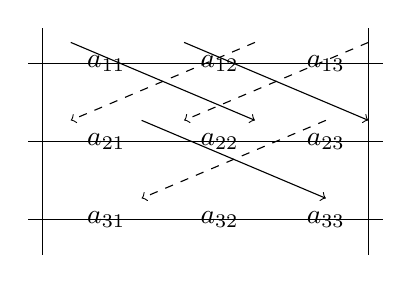
\begin{tikzpicture}[scale=0.9]
% three horizontal lines
\draw (0,2.6) -- (5.0,2.6);
\draw (0,1.5) -- (5.0,1.5);
\draw (0,0.4) -- (5.0,0.4);
% vertical-ish separator lines
\draw (0.2,3.1) -- (0.2,-0.1);
\draw (4.8,3.1) -- (4.8,-0.1);
% nodes
\node at (1.1,2.6) {$a_{11}$};
\node at (2.7,2.6) {$a_{12}$};
\node at (4.2,2.6) {$a_{13}$};
\node at (1.1,1.5) {$a_{21}$};
\node at (2.7,1.5) {$a_{22}$};
\node at (4.2,1.5) {$a_{23}$};
\node at (1.1,0.4) {$a_{31}$};
\node at (2.7,0.4) {$a_{32}$};
\node at (4.2,0.4) {$a_{33}$};
% solid arrows (down-right)
\draw[->] (0.6,2.9) -- (3.2,1.8);
\draw[->] (2.2,2.9) -- (4.8,1.8);
\draw[->] (1.6,1.8) -- (4.2,0.7);
% dashed arrows (down-left)
\draw[dashed,->] (4.8,2.9) -- (2.2,1.8);
\draw[dashed,->] (3.2,2.9) -- (0.6,1.8);
\draw[dashed,->] (4.2,1.8) -- (1.6,0.7);
\end{tikzpicture}
\end{mvfigure}

\mvthm{定义 2A.25}{如果把一个矩阵的行看成向量(即行向量),矩阵的行秩就是线性无关的行的最大数目.如果把矩阵的列看成向量,一个矩阵的列秩是它的列集合的秩.}

例如,设矩阵
\[
\bm{A} = \begin{bmatrix} 1 & 1 & 1 \\ 2 & 5 & -1 \\ 0 & 1 & -1 \end{bmatrix}
\]

把 $\bm{A}$ 的行写成向量形式,定义 2A.6 后的例子已证明它们是线性相关的.注意 $\bm{A}$ 的列秩也是 2,因为

%% ===== pg-084 =====

% ---- pg-084 （书页 72） ----

\[
-2\begin{bmatrix} 1 \\ 2 \\ 0 \end{bmatrix} + 5\begin{bmatrix} 1 \\ 1 \\ 1 \end{bmatrix} + \begin{bmatrix} -1 \\ -1 \\ -1 \end{bmatrix} = \begin{bmatrix} 0 \\ 0 \\ 0 \end{bmatrix}
\]

而第 1 列和第 2 列是线性无关的.正如下面结论所指出的,这并非巧合.

\mvthm{结论 2A.6}{一个矩阵的行秩和列秩是相等的.}

因此,一个矩阵的秩既是行秩也是列秩.

\mvthm{定义 2A.26}{对方阵 $\bm{A}$,如果 $\bm{A}\,\bm{x}_{(k\times 1)} = \bm{0}_{(k\times 1)}$ 意味着 $\bm{x}_{(k\times 1)} = \bm{0}_{(k\times 1)}$,则称此方阵是非奇异的.如果一个矩阵不是非奇异的,则称它是奇异的.等价地说,如果一个方阵的秩等于它的行(或列)数,则此方阵是非奇异的.}

注意 $\bm{A}\bm{x} = x_1\bm{a}_1 + x_2\bm{a}_2 + \cdots + x_k\bm{a}_k$,其中 $\bm{a}_i$ 是 $\bm{A}$ 的第 $i$ 列,于是 $\bm{A}$ 是非奇异 的条件恰好就是 $\bm{A}$ 的列向量线性无关.

\mvthm{结论 2A.7}{设 $\bm{A}$ 是一个非奇异的 $k\times k$ 维方阵,则存在唯一的 $k\times k$ 矩阵 $\bm{B}$,使得}
\[
\bm{A}\bm{B} = \bm{B}\bm{A} = \bm{I}
\]
其中 $\bm{I}$ 是 $k\times k$ 单位矩阵.

\mvthm{定义 2A.27}{若 $\bm{B}$ 满足 $\bm{A}\bm{B}=\bm{B}\bm{A}=\bm{I}$,称 $\bm{B}$ 为 $\bm{A}$ 的逆并用 $\bm{A}^{-1}$ 表示.事实上,如果 $\bm{B}\bm{A}=\bm{I}$ 或 $\bm{A}\bm{B}=\bm{I}$,则 $\bm{B}=\bm{A}^{-1}$,且两个乘积必定等于 $\bm{I}$.}

例如,
\[
\bm{A} = \begin{bmatrix} 2 & 3 \\ 1 & 5 \end{bmatrix} \qquad \text{有} \qquad
\bm{A}^{-1} = \begin{bmatrix} \dfrac{5}{7} & -\dfrac{3}{7} \\[8pt] -\dfrac{1}{7} & \dfrac{2}{7} \end{bmatrix}
\]

因为
\[
\begin{bmatrix} 2 & 3 \\ 1 & 5 \end{bmatrix}\begin{bmatrix} \dfrac{5}{7} & -\dfrac{3}{7} \\[8pt] -\dfrac{1}{7} & \dfrac{2}{7} \end{bmatrix}
= \begin{bmatrix} \dfrac{5}{7} & -\dfrac{3}{7} \\[8pt] -\dfrac{1}{7} & \dfrac{2}{7} \end{bmatrix}\begin{bmatrix} 2 & 3 \\ 1 & 5 \end{bmatrix}
= \begin{bmatrix} 1 & 0 \\ 0 & 1 \end{bmatrix}
\]

\mvthm{结论 2A.8}{}

(a) 任一 $2\times2$ 矩阵
\[
\bm{A} = \begin{bmatrix} a_{11} & a_{12} \\ a_{21} & a_{22} \end{bmatrix}
\]

的逆是
\[
\bm{A}^{-1} = \frac{1}{|\bm{A}|}\begin{bmatrix} a_{22} & -a_{12} \\ -a_{21} & a_{11} \end{bmatrix}
\]

(b) 任一 $3\times3$ 矩阵
\[
\bm{A} = \begin{bmatrix} a_{11} & a_{12} & a_{13} \\ a_{21} & a_{22} & a_{23} \\ a_{31} & a_{32} & a_{33} \end{bmatrix}
\]

的逆是

%% ===== pg-085 =====

% ---- pg-085 （书页 73） ----

\[
\bm{A}^{-1} = \frac{1}{|\bm{A}|}
\begin{bmatrix}
\left|\begin{matrix} a_{22} & a_{23} \\ a_{32} & a_{33} \end{matrix}\right| & -\left|\begin{matrix} a_{12} & a_{13} \\ a_{32} & a_{33} \end{matrix}\right| & \left|\begin{matrix} a_{12} & a_{13} \\ a_{22} & a_{23} \end{matrix}\right| \\[12pt]
-\left|\begin{matrix} a_{21} & a_{23} \\ a_{31} & a_{33} \end{matrix}\right| & \left|\begin{matrix} a_{11} & a_{13} \\ a_{31} & a_{33} \end{matrix}\right| & -\left|\begin{matrix} a_{11} & a_{13} \\ a_{21} & a_{23} \end{matrix}\right| \\[12pt]
\left|\begin{matrix} a_{21} & a_{22} \\ a_{31} & a_{32} \end{matrix}\right| & -\left|\begin{matrix} a_{11} & a_{12} \\ a_{31} & a_{32} \end{matrix}\right| & \left|\begin{matrix} a_{11} & a_{12} \\ a_{21} & a_{22} \end{matrix}\right|
\end{bmatrix}
\]

在 (a) 和 (b) 中,如果逆存在,显然 $|\bm{A}| \neq 0$.

(c) 一般的,$\bm{A}^{-1}$ 的第 $j,i$ 个元素为 $[|\bm{A}_{ij}|\,/\,|\bm{A}|]\,(-1)^{i+j}$,其中 $\bm{A}_{ij}$ 是从 $\bm{A}$ 中除去第 $i$ 行和第 $j$ 列后得到的矩阵.

\mvthm{结论 2A.9}{对一个 $k\times k$ 维的方阵 $\bm{A}$,有如下等价表述:}

(a) $\bm{A}\,\bm{x}_{(k\times 1)} = \bm{0}_{(k\times 1)}$ 意味着 $\bm{x}_{(k\times 1)} = \bm{0}_{(k\times 1)}$ ($\bm{A}$ 是非奇异的).

(b) $|\bm{A}| \neq 0$.

(c) 存在一个矩阵 $\bm{A}^{-1}$,使得 $\bm{A}\bm{A}^{-1} = \bm{A}^{-1}\bm{A} = \bm{I}_{(k\times k)}$.

\mvthm{结论 2A.10}{设 $\bm{A}$ 和 $\bm{B}$ 是同维数方阵,且存在逆矩阵,则如下性质成立:}

(a) $(\bm{A}^{-1})' = (\bm{A}')^{-1}$

(b) $(\bm{A}\bm{B})^{-1} = \bm{B}^{-1}\bm{A}^{-1}$

行列式具有如下性质.

\mvthm{结论 2A.11}{设 $\bm{A}$ 和 $\bm{B}$ 是 $k\times k$ 方阵.}

(a) $|\bm{A}| = |\bm{A}'|$

(b) 若 $\bm{A}$ 中一行(列)的每一元素均为零,则 $|\bm{A}| = 0$

(c) 若 $\bm{A}$ 的任两行(列)相同,则 $|\bm{A}| = 0$

(d) 若 $\bm{A}$ 是非奇异的,则 $|\bm{A}| = 1/|\bm{A}^{-1}|$,即 $|\bm{A}|\,|\bm{A}^{-1}| = 1$.

(e) $|\bm{A}\bm{B}| = |\bm{A}|\,|\bm{B}|$

(f) $|c\bm{A}| = c^k|\bm{A}|$,其中 $c$ 为标量.

结论 2A.9 和 2A.11 的部分证明参看文献 [6],这些证明有的相当复杂,超出了本书的范围.

\mvthm{定义 2A.28}{设 $\bm{A} = \{a_{ij}\}$ 是 $k\times k$ 方阵,矩阵 $\bm{A}$ 的迹记做 $\operatorname{tr}(\bm{A})$,它是对角线上元素的和,即}
\[
\operatorname{tr}(\bm{A}) = \sum_{i=1}^{k}a_{ii}
\]

\mvthm{结论 2A.12}{设 $\bm{A}$ 和 $\bm{B}$ 是 $k\times k$ 矩阵且 $c$ 为标量.}

(a) $\operatorname{tr}(c\bm{A}) = c\operatorname{tr}(\bm{A})$

(b) $\operatorname{tr}(\bm{A}\pm\bm{B}) = \operatorname{tr}(\bm{A}) \pm \operatorname{tr}(\bm{B})$

(c) $\operatorname{tr}(\bm{A}\bm{B}) = \operatorname{tr}(\bm{B}\bm{A})$

(d) $\operatorname{tr}(\bm{B}^{-1}\bm{A}\bm{B}) = \operatorname{tr}(\bm{A})$

(e) $\operatorname{tr}(\bm{A}\bm{A}') = \sum_{i=1}^{k}\sum_{j=1}^{k}a_{ij}^2$

\mvthm{定义 2A.29}{把方阵 $\bm{A}$ 的行看成是向量,若行与行互相垂直且都为单位长度,则说 $\bm{A}$ 是正交的.即 $\bm{A}\bm{A}' = \bm{I}$.}

%% ===== pg-086 =====

% ---- pg-086 （书页 74） ----

\mvbold{结论 2A.13}\quad 当且仅当 $\bm{A}^{-1} = \bm{A}'$ 时,矩阵 $\bm{A}$ 是正交的.对于一个正交矩阵, $\bm{A}\bm{A}' = \bm{A}'\bm{A} = \bm{I}$.因此,列向量互相垂直且为单位长度. \ $\blacksquare$

下面是正交矩阵的一个例子

\[
\bm{A} = \begin{bmatrix}
-\dfrac{1}{2} & \dfrac{1}{2} & \dfrac{1}{2} & \dfrac{1}{2} \\[3mm]
\dfrac{1}{2} & -\dfrac{1}{2} & \dfrac{1}{2} & \dfrac{1}{2} \\[3mm]
\dfrac{1}{2} & \dfrac{1}{2} & -\dfrac{1}{2} & \dfrac{1}{2} \\[3mm]
\dfrac{1}{2} & \dfrac{1}{2} & \dfrac{1}{2} & -\dfrac{1}{2}
\end{bmatrix}
\]

显然, $\bm{A} = \bm{A}'$,因此, $\bm{A}\bm{A}' = \bm{A}'\bm{A} = \bm{A}\bm{A}$.我们验证 $\bm{A}\bm{A} = \bm{I} = \bm{A}\bm{A}' = \bm{A}'\bm{A}$,或

\[
\underbrace{\begin{bmatrix}
-\dfrac{1}{2} & \dfrac{1}{2} & \dfrac{1}{2} & \dfrac{1}{2} \\[3mm]
\dfrac{1}{2} & -\dfrac{1}{2} & \dfrac{1}{2} & \dfrac{1}{2} \\[3mm]
\dfrac{1}{2} & \dfrac{1}{2} & -\dfrac{1}{2} & \dfrac{1}{2} \\[3mm]
\dfrac{1}{2} & \dfrac{1}{2} & \dfrac{1}{2} & -\dfrac{1}{2}
\end{bmatrix}}_{\bm{A}}
\underbrace{\begin{bmatrix}
-\dfrac{1}{2} & \dfrac{1}{2} & \dfrac{1}{2} & \dfrac{1}{2} \\[3mm]
\dfrac{1}{2} & -\dfrac{1}{2} & \dfrac{1}{2} & \dfrac{1}{2} \\[3mm]
\dfrac{1}{2} & \dfrac{1}{2} & -\dfrac{1}{2} & \dfrac{1}{2} \\[3mm]
\dfrac{1}{2} & \dfrac{1}{2} & \dfrac{1}{2} & -\dfrac{1}{2}
\end{bmatrix}}_{\bm{A}}
=
\underbrace{\begin{bmatrix} 1 & 0 & 0 & 0 \\ 0 & 1 & 0 & 0 \\ 0 & 0 & 1 & 0 \\ 0 & 0 & 0 & 1 \end{bmatrix}}_{\bm{I}}
\]

于是 $\bm{A}' = \bm{A}^{-1}$,且 $\bm{A}$ 必定是一个正交阵.

通过特征值和特征向量等量,可以最充分地理解方阵.

\mvbold{定义 2A.30}\quad 设 $\bm{A}$ 是 $k \times k$ 方阵, $\bm{I}$ 是 $k \times k$ 单位阵,则满足多项式方程 $|\bm{A} - \lambda\bm{I}| = 0$ 的标量 $\lambda_1, \lambda_2, \cdots, \lambda_k$ 称为矩阵 $\bm{A}$ 的特征值(或特征根).方程 $|\bm{A} - \lambda\bm{I}| = 0$ ($\lambda$ 的函数)称为特征方程.

例如,设

\[
\bm{A} = \begin{bmatrix} 1 & 0 \\ 1 & 3 \end{bmatrix}
\]

则

\begin{equation*}
\begin{aligned}
|\bm{A} - \lambda\bm{I}| &= \left|\begin{bmatrix} 1 & 0 \\ 1 & 3 \end{bmatrix} - \lambda\begin{bmatrix} 1 & 0 \\ 0 & 1 \end{bmatrix}\right| \\
&= \begin{vmatrix} 1 - \lambda & 0 \\ 1 & 3 - \lambda \end{vmatrix} = (1 - \lambda)(3 - \lambda) = 0
\end{aligned}
\end{equation*}

意味着有两个根, $\lambda_1 = 1$ 和 $\lambda_2 = 3$. $\bm{A}$ 的特征值是 3 和 1.设

\[
\bm{A} = \begin{bmatrix} 13 & -4 & 2 \\ -4 & 13 & -2 \\ 2 & -2 & 10 \end{bmatrix}
\]

则方程

\[
|\bm{A} - \lambda\bm{I}| = \begin{vmatrix} 13 - \lambda & -4 & 2 \\ -4 & 13 - \lambda & -2 \\ 2 & -2 & 10 - \lambda \end{vmatrix} = -\lambda^3 + 36\lambda^2 - 405\lambda + 1\,458 = 0
\]

有三个根: $\lambda_1 = 9$, $\lambda_2 = 9$ 和 $\lambda_3 = 18$;即 9, 9 和 18 是 $\bm{A}$ 的特征值.

%% ===== pg-087 =====

% ---- pg-087 （书页 75） ----

\mvbold{定义 2A.31}\quad 设 $\bm{A}$ 是一个 $k \times k$ 维矩阵, $\lambda$ 是 $\bm{A}$ 的一个特征值.如果非零向量 $\bm{x}_{(k \times 1)}$($\bm{x} \neq \bm{0}$)满足

\[
\bm{A}\bm{x} = \lambda\bm{x}
\]

则称 $\bm{x}$ 是矩阵 $\bm{A}$ 的相应于特征值 $\lambda$ 的特征向量.

$\lambda$ 是特征值-特征向量方程的解的一个等价条件是 $|\bm{A} - \lambda\bm{I}| = 0$.这是因为,对于某个 $\lambda$ 和 $\bm{x} \neq \bm{0}$, $\bm{A}\bm{x} = \lambda\bm{x}$ 意味着

\[
\bm{0} = (\bm{A} - \lambda\bm{I})\bm{x} = x_1 \cdot \text{列}_1(\bm{A} - \lambda\bm{I}) + \cdots + x_k \cdot \text{列}_k(\bm{A} - \lambda\bm{I})
\]

也就是说, $\bm{A} - \lambda\bm{I}$ 的列向量是线性相关的,故由结论 2A.9(b)可断言 $|\bm{A} - \lambda\bm{I}| = 0$.按照定义 2A.30,我们指出

\[
\bm{A} = \begin{bmatrix} 1 & 0 \\ 1 & 3 \end{bmatrix}
\]

的特征值是 $\lambda_1 = 1$ 和 $\lambda_2 = 3$.对应于这些特征值的特征向量可以通过解下述方程来确定：

\[
\begin{bmatrix} 1 & 0 \\ 1 & 3 \end{bmatrix}\begin{bmatrix} x_1 \\ x_2 \end{bmatrix} = 1\begin{bmatrix} x_1 \\ x_2 \end{bmatrix}
\]
\[
\bm{A}\bm{x} = \lambda_1\bm{x}
\]
\[
\begin{bmatrix} 1 & 0 \\ 1 & 3 \end{bmatrix}\begin{bmatrix} x_1 \\ x_2 \end{bmatrix} = 3\begin{bmatrix} x_1 \\ x_2 \end{bmatrix}
\]
\[
\bm{A}\bm{x} = \lambda_2\bm{x}
\]

从第一式

\[
\begin{aligned}
x_1 &= x_1 \\
x_1 + 3x_2 &= x_2
\end{aligned}
\]

或

\[
x_1 = -2x_2
\]

可求出 $x_1$ 和 $x_2$ 的许多解.

令 $x_2 = 1$(任意的),得出 $x_1 = -2$,因此,

\[
\bm{x} = \begin{bmatrix} -2 \\ 1 \end{bmatrix}
\]

是对应于特征值 1 的一个特征向量.从第二式,

\[
\begin{aligned}
x_1 &= 3x_1 \\
x_1 + 3x_2 &= 3x_2
\end{aligned}
\]

可以推出 $x_1 = 0$ 和 $x_2 = 1$(任意地),因此,

\[
\bm{x} = \begin{bmatrix} 0 \\ 1 \end{bmatrix}
\]

是特征值 3 对应的特征向量.通常习惯于确定一个特征向量使它为单位长度.即,如果 $\bm{A}\bm{x} = \lambda\bm{x}$,取 $\bm{e} = \bm{x}/\sqrt{\bm{x}'\bm{x}}$ 作为 $\lambda$ 对应的特征向量.例如, $\lambda_1 = 1$ 时其特征向量为 $[-2/\sqrt{5}, 1/\sqrt{5}]'$.

\mvbold{定义 2A.32}\quad $k$ 个变量 $x_1, x_2, \cdots, x_k$ 的二次型 $Q(\bm{x})$ 为 $Q(\bm{x}) = \bm{x}'\bm{A}\bm{x}$,其中 $\bm{x}' = [x_1, x_2, \cdots, x_k]$,且 $\bm{A}$ 是一个 $k \times k$ 对称矩阵.

注意二次型可以写做 $Q(\bm{x}) = \sum\limits_{i=1}^{k}\sum\limits_{j=1}^{k}a_{ij}x_i x_j$.例如,

%% ===== pg-088 =====

% ---- pg-088 （书页 76） ----

\[
Q(\bm{x}) = [x_1 \quad x_2]\begin{bmatrix} 1 & 1 \\ 1 & 1 \end{bmatrix}\begin{bmatrix} x_1 \\ x_2 \end{bmatrix} = x_1^2 + 2x_1x_2 + x_2^2
\]
\[
Q(\bm{x}) = [x_1 \quad x_2 \quad x_3]\begin{bmatrix} 1 & 3 & 0 \\ 3 & -1 & -2 \\ 0 & -2 & 2 \end{bmatrix}\begin{bmatrix} x_1 \\ x_2 \\ x_3 \end{bmatrix} = x_1^2 + 6x_1x_2 - x_2^2 - 4x_2x_3 + 2x_3^2
\]

任何对称方阵可以由它的特征值和特征向量重构.这个特殊的表达式揭示了依据特征值的相对大小和特征向量的方向,每一个特征值-特征向量对的相对重要性.

\mvbold{结论 2A.14}\quad （谱分解）设 $\bm{A}$ 是 $k \times k$ 对称矩阵,则 $\bm{A}$ 可用它的 $k$ 个特征值-特征向量对 $(\lambda_i, \bm{e}_i)$ 表示为

\[
\bm{A} = \sum_{i=1}^{k}\lambda_i\bm{e}_i\bm{e}_i' \qquad \blacksquare
\]

假如,设

\[
\bm{A} = \begin{bmatrix} 2.2 & 0.4 \\ 0.4 & 2.8 \end{bmatrix}
\]

则

\[
|\bm{A} - \lambda\bm{I}| = \lambda^2 - 5\lambda + 6.16 - 0.16 = (\lambda - 3)(\lambda - 2)
\]

因此 $\bm{A}$ 的特征值 $\lambda_1 = 3$ 和 $\lambda_2 = 2$.相应的特征向量分别为 $\bm{e}_1' = [1/\sqrt{5}, 2/\sqrt{5}]$ 和 $\bm{e}_2' = [2/\sqrt{5}, -1/\sqrt{5}]$.于是,

\begin{equation*}
\begin{aligned}
\bm{A} &= \begin{bmatrix} 2.2 & 0.4 \\ 0.4 & 2.8 \end{bmatrix} = 3\begin{bmatrix} \dfrac{1}{\sqrt{5}} \\[2mm] \dfrac{2}{\sqrt{5}} \end{bmatrix}\begin{bmatrix} \dfrac{1}{\sqrt{5}} & \dfrac{2}{\sqrt{5}} \end{bmatrix} + 2\begin{bmatrix} \dfrac{2}{\sqrt{5}} \\[2mm] -\dfrac{1}{\sqrt{5}} \end{bmatrix}\begin{bmatrix} \dfrac{2}{\sqrt{5}} & -\dfrac{1}{\sqrt{5}} \end{bmatrix} \\
&= \begin{bmatrix} 0.6 & 1.2 \\ 1.2 & 2.4 \end{bmatrix} + \begin{bmatrix} 1.6 & -0.8 \\ -0.8 & 0.4 \end{bmatrix}
\end{aligned}
\end{equation*}

谱分解的思想可以推广到给出长方阵而不只是方阵的分解.若 $\bm{A}$ 是一个长方阵,则 $\bm{A}$ 的展开式中的向量分别是方阵 $\bm{A}\bm{A}'$ 和 $\bm{A}'\bm{A}$ 的特征向量.

\mvbold{结论 2A.15}\quad （奇异值分解）设 $\bm{A}$ 是 $m \times k$ 的实数矩阵,则存在一个 $m \times m$ 正交阵 $\bm{U}$ 和一个 $k \times k$ 正交阵 $\bm{V}$ 使得

\[
\bm{A} = \bm{U}\bm{\Delta}\bm{V}'
\]

此处 $m \times k$ 矩阵 $\bm{\Delta}$ 中, $(i,i)$ 元素 $\lambda_i \geqslant 0$, $i = 1, 2, \cdots, \min(m,k)$,其他元素是零.正数 $\lambda_i$ 称为 $\bm{A}$ 的奇异值. \ $\blacksquare$

奇异值分解也能表示为一个基于 $\bm{A}$ 的秩 $r$ 的矩阵展开式.具体地说,存在 $r$ 个正数 $\lambda_1, \lambda_2, \cdots, \lambda_r$, $r$ 个正交 $m \times 1$ 单位向量 $\bm{u}_1, \bm{u}_2, \cdots, \bm{u}_r$ 和 $r$ 个正交 $k \times 1$ 单位向量 $\bm{v}_1, \bm{v}_2, \cdots, \bm{v}_r$,使得

\[
\bm{A} = \sum_{i=1}^{r}\lambda_i\bm{u}_i\bm{v}_i' = \bm{U}_r\bm{\Delta}_r\bm{V}_r'
\]

其中 $\bm{U}_r = [\bm{u}_1, \bm{u}_2, \cdots, \bm{u}_r]$, $\bm{V}_r = [\bm{v}_1, \bm{v}_2, \cdots, \bm{v}_r]$,而 $\bm{\Delta}_r$ 是一个对角元素为 $\lambda_i$ 的 $r \times r$ 对角阵.

这里 $\bm{A}\bm{A}'$ 有特征值-特征向量对 $(\lambda_i^2, \bm{u}_i)$,于是,

\[
\bm{A}\bm{A}'\bm{u}_i = \lambda_i^2\bm{u}_i
\]

且 $\lambda_1^2, \lambda_2^2, \cdots, \lambda_r^2 > 0 = \lambda_{r+1}^2, \lambda_{r+2}^2, \cdots, \lambda_m^2$(对 $m > k$).因而, $\bm{v}_i = \lambda_i^{-1}\bm{A}'\bm{u}_i$.换言之, $\bm{v}_i$ 是 $\bm{A}'\bm{A}$ 的对应于同一个非零特征值 $\lambda_i^2$ 的特征向量.

%% ===== pg-089 =====

% ---- pg-089 （书页 77） ----

奇异值分解的矩阵展开式用满维矩阵 $\bm{U}, \bm{V}, \bm{\Delta}$ 可写为

\[
\bm{A}_{(m \times k)} = \bm{U}_{(m \times m)}\bm{\Delta}_{(m \times k)}\bm{V}_{(k \times k)}'
\]

其中 $\bm{U}$ 的列为 $\bm{A}\bm{A}'$ 的 $m$ 个正交特征向量, $\bm{V}$ 的列为 $\bm{A}'\bm{A}$ 的 $k$ 个正交特征向量, $\bm{\Delta}$ 如结论 2A.15 中所示.

设

\[
\bm{A} = \begin{bmatrix} 3 & 1 & 1 \\ -1 & 3 & 1 \end{bmatrix}
\]

则

\[
\bm{A}\bm{A}' = \begin{bmatrix} 3 & 1 & 1 \\ -1 & 3 & 1 \end{bmatrix}\begin{bmatrix} 3 & -1 \\ 1 & 3 \\ 1 & 1 \end{bmatrix} = \begin{bmatrix} 11 & 1 \\ 1 & 11 \end{bmatrix}
\]

可以验证 $\bm{A}\bm{A}'$ 的特征值 $\gamma = \lambda^2$ 满足方程 $\gamma^2 - 22\gamma + 120 = (\gamma - 12)(\gamma - 10)$,因此,特征值是 $\gamma_1 = \lambda_1^2 = 12$ 和 $\gamma_2 = \lambda_2^2 = 10$,对应的特征向量分别是 $\bm{u}_1' = \left[\dfrac{1}{\sqrt{2}}, \dfrac{1}{\sqrt{2}}\right]$ 和 $\bm{u}_2' = \left[\dfrac{1}{\sqrt{2}}, -\dfrac{1}{\sqrt{2}}\right]$.

又

\[
\bm{A}'\bm{A} = \begin{bmatrix} 3 & -1 \\ 1 & 3 \\ 1 & 1 \end{bmatrix}\begin{bmatrix} 3 & 1 & 1 \\ -1 & 3 & 1 \end{bmatrix} = \begin{bmatrix} 10 & 0 & 2 \\ 0 & 10 & 4 \\ 2 & 4 & 2 \end{bmatrix}
\]

所以 $|\bm{A}'\bm{A} - \gamma\bm{I}| = -\gamma^3 - 22\gamma^2 - 120\gamma = -\gamma(\gamma - 12)(\gamma - 10)$,且特征值为 $\gamma_1 = \lambda_1^2 = 12$, $\gamma_2 = \lambda_2^2 = 10$ 及 $\gamma_3 = \lambda_3^2 = 0$.非零特征值与 $\bm{A}\bm{A}'$ 的非零特征值是相同的.用计算机算出特征向量为 $\bm{v}_1' = \left[\dfrac{1}{\sqrt{6}}, \dfrac{2}{\sqrt{6}}, \dfrac{1}{\sqrt{6}}\right]$, $\bm{v}_2' = \left[\dfrac{2}{\sqrt{5}}, -\dfrac{1}{\sqrt{5}}, 0\right]$ 及 $\bm{v}_3' = \left[\dfrac{1}{\sqrt{30}}, \dfrac{2}{\sqrt{30}}, -\dfrac{5}{\sqrt{30}}\right]$.对特征向量 $\bm{v}_1$ 和 $\bm{v}_2$ 可以进行检验：

\[
\bm{A}'\bm{A}\bm{v}_1 = \begin{bmatrix} 10 & 0 & 2 \\ 0 & 10 & 4 \\ 2 & 4 & 2 \end{bmatrix}\begin{bmatrix} 1 \\ 2 \\ 1 \end{bmatrix}\frac{1}{\sqrt{6}} \times \frac{1}{\sqrt{6}} = 12 \times \frac{1}{\sqrt{6}}\begin{bmatrix} 1 \\ 2 \\ 1 \end{bmatrix} = \lambda_1^2\bm{v}_1
\]
\[
\bm{A}'\bm{A}\bm{v}_2 = \begin{bmatrix} 10 & 0 & 2 \\ 0 & 10 & 4 \\ 2 & 4 & 2 \end{bmatrix}\begin{bmatrix} 2 \\ -1 \\ 0 \end{bmatrix}\frac{1}{\sqrt{5}} = 10 \times \frac{1}{\sqrt{5}}\begin{bmatrix} 2 \\ -1 \\ 0 \end{bmatrix} = \lambda_2^2\bm{v}_2
\]

选取 $\lambda_1 = \sqrt{12}$ 和 $\lambda_2 = \sqrt{10}$,我们求得 $\bm{A}$ 的奇异值分解是

\begin{equation*}
\begin{aligned}
\bm{A} &= \begin{bmatrix} 3 & 1 & 1 \\ -1 & 3 & 1 \end{bmatrix} \\
&= \sqrt{12}\begin{bmatrix} \dfrac{1}{\sqrt{2}} \\[2mm] \dfrac{1}{\sqrt{2}} \end{bmatrix}\left[\frac{1}{\sqrt{6}} \quad \frac{2}{\sqrt{6}} \quad \frac{1}{\sqrt{6}}\right] + \sqrt{10}\begin{bmatrix} \dfrac{1}{\sqrt{2}} \\[2mm] -\dfrac{1}{\sqrt{2}} \end{bmatrix}\left[\frac{2}{\sqrt{5}} \quad -\frac{1}{\sqrt{5}} \quad 0\right]
\end{aligned}
\end{equation*}

可以完成右边的计算来检验该等式.

奇异值分解与一个用低维矩阵逼近三角矩阵的结果有紧密的联系,该工作主要由 Eckart 和 Young(见文献[2])完成.如果做一个 $m \times k$ 矩阵 $\bm{A}$ 可以用具有相同维度但秩更低的矩阵 $\bm{B}$ 来逼近,差的平方和为

%% ===== pg-090 =====

\begin{equation}
\sum_{i=1}^{m}\sum_{j=1}^{k}(a_{ij}-b_{ij})^{2}=\operatorname{tr}\left[(\mathbf{A}-\mathbf{B})(\mathbf{A}-\mathbf{B})'\right]
\end{equation}

\noindent\textbf{结论 2A.16}\quad $\mathbf{A}$ 是 $m\times k(m\ge k)$ 阶实矩阵, 并且有奇异值分解 $\mathbf{U}\boldsymbol{\Delta}\mathbf{V}'$, 设 $s<k=\mathbf{A}$ 的秩, 则
$\mathbf{B}=\sum_{i=1}^{s}\lambda_{i}\mathbf{u}_{i}\mathbf{v}_{i}'$ 是 $\mathbf{A}$ 的秩-$s$ 最小二乘逼近, 使得在所有秩小于 $s$ 的 $m\times k$ 阶矩阵 $\mathbf{B}$ 中, $\operatorname{tr}\left[(\mathbf{A}-\mathbf{B})(\mathbf{A}-\mathbf{B})'\right]$ 最小, 且最小值或者逼近误差是 $\sum_{i=s+1}^{k}\lambda_{i}^{2}$.\hfill$\blacksquare$

\medskip
为了得到以上的结论, 我们利用 $\mathbf{U}\mathbf{U}'=\mathbf{I}_{m}$ 和 $\mathbf{V}\mathbf{V}'=\mathbf{I}_{k}$, 然后将平方和写成
\begin{align*}
\operatorname{tr}\left[(\mathbf{A}-\mathbf{B})(\mathbf{A}-\mathbf{B})'\right]
&=\operatorname{tr}\left[\mathbf{U}\mathbf{U}'(\mathbf{A}-\mathbf{B})\mathbf{V}\mathbf{V}'(\mathbf{A}-\mathbf{B})'\right]\\
&=\operatorname{tr}\left[\mathbf{U}'(\mathbf{A}-\mathbf{B})\mathbf{V}\mathbf{V}'(\mathbf{A}-\mathbf{B})'\mathbf{U}\right]\\
&=\operatorname{tr}\left[(\boldsymbol{\Delta}-\mathbf{C})(\boldsymbol{\Delta}-\mathbf{C})'\right]
=\sum_{i=1}^{m}\sum_{j=1}^{k}(\lambda_{ij}-c_{ij})^{2}
=\sum_{i=1}^{k}(\lambda_{i}-c_{ii})^{2}+\sum_{i\ne j}\sum_{i\ne j}c_{ij}^{2}
\end{align*}
这里 $\mathbf{C}=\mathbf{U}'\mathbf{B}\mathbf{V}$, 显然, 当 $\mathbf{C}$ 取如下值时取到最小值, 即当 $i\ne j$ 时, 取 $c_{ij}=0$ 且对 $s$ 个最大奇异值取 $c_{ii}=\lambda_{i}$. 而其他的 $c_{ii}=0$. 这就是说, $\mathbf{U}'\mathbf{B}\mathbf{V}=\boldsymbol{\Delta}_{s}$ 或 $\mathbf{B}=\sum_{i=1}^{s}\lambda_{i}\mathbf{u}_{i}\mathbf{v}_{i}'$.

\vspace{6pt}
{\large\bfseries 练习}

\medskip
\noindent 2.1\quad 设 $\mathbf{x}'=[5,1,3]$ 和 $\mathbf{y}'=[-1,3,1]$.

\noindent (a) 画两个向量的图形.

\noindent (b) 求 (i) $\mathbf{x}$ 的长度, (ii) $\mathbf{x}$ 和 $\mathbf{y}$ 之间的夹角, (iii) $\mathbf{y}$ 在 $\mathbf{x}$ 上的投影.

\noindent (c) 因为 $\bar{x}=3$ 和 $\bar{y}=1$, 画出 $[5-3,1-3,3-3]=[2,-2,0]$ 和 $[-1-1,3-1,1-1]=[-2,2,0]$.

\medskip
\noindent 2.2\quad 已知矩阵
\[
\mathbf{A}=\begin{bmatrix}-1&3\\4&2\end{bmatrix},\quad
\mathbf{B}=\begin{bmatrix}4&-3\\1&-2\\-2&0\end{bmatrix}\ \text{及}\
\mathbf{C}=\begin{bmatrix}5\\-4\\2\end{bmatrix}
\]
做下述指定的乘法.
\begin{tabbing}
\hspace*{2em}\=(a)\quad \= $5\mathbf{A}$\\[2pt]
\>(b)\> $\mathbf{B}\mathbf{A}$\\[2pt]
\>(c)\> $\mathbf{A}'\mathbf{B}'$\\[2pt]
\>(d)\> $\mathbf{C}'\mathbf{B}$\\[2pt]
\>(e)\> $\mathbf{A}\mathbf{B}$ 有定义吗?
\end{tabbing}

\medskip
\noindent 2.3\quad 当
\[
\mathbf{A}=\begin{bmatrix}2&1\\1&3\end{bmatrix},\quad
\mathbf{B}=\begin{bmatrix}1&4&2\\5&0&3\end{bmatrix}\ \text{及}\
\mathbf{C}=\begin{bmatrix}1&4\\3&2\end{bmatrix}
\]
时, 证明转置的下列性质:
\begin{tabbing}
\hspace*{2em}\=(a)\quad \= $(\mathbf{A}')'=\mathbf{A}$\\[2pt]
\>(b)\> $(\mathbf{C}^{-1})'=(\mathbf{C}^{-1})'$\\[2pt]
\>(c)\> $(\mathbf{A}\mathbf{B})'=\mathbf{B}'\mathbf{A}'$\\[2pt]
\>(d)\> 对一般的 $\mathbf{A}$ 和 $\mathbf{B}$, $(\mathbf{A}\mathbf{B})'=\mathbf{B}'\mathbf{A}'$.
\end{tabbing}

\medskip
\noindent 2.4\quad 当 $\mathbf{A}^{-1}$ 和 $\mathbf{B}^{-1}$ 存在时, 证明下列性质:

%% ===== pg-091 =====

\begin{tabbing}
\hspace*{2em}\=(a)\quad \= $(\mathbf{A}')^{-1}=(\mathbf{A}^{-1})'$\\[2pt]
\>(b)\> $(\mathbf{A}\mathbf{B})^{-1}=\mathbf{B}^{-1}\mathbf{A}^{-1}$
\end{tabbing}

\noindent 提示: 由 $\mathbf{A}\mathbf{A}^{-1}=\mathbf{I},\mathbf{I}=\mathbf{I}'$ 及 $(\mathbf{A}\mathbf{A}^{-1})'=(\mathbf{A}^{-1})'\mathbf{A}'$ 可证明 (a). 由 $(\mathbf{B}^{-1}\mathbf{A}^{-1})\mathbf{A}\mathbf{B}=\mathbf{B}^{-1}(\mathbf{A}^{-1}\mathbf{A})\mathbf{B}=\mathbf{B}^{-1}\mathbf{B}=\mathbf{I}$ 可证明 (b).

\medskip
\noindent 2.5\quad 检验
\[
\mathbf{Q}=\begin{bmatrix}\dfrac{5}{13}&\dfrac{12}{13}\\[6pt]-\dfrac{12}{13}&\dfrac{5}{13}\end{bmatrix}
\]
是一个正交矩阵.

\medskip
\noindent 2.6\quad 设
\[
\mathbf{A}=\begin{bmatrix}9&-2\\-2&6\end{bmatrix}
\]
\begin{tabbing}
\hspace*{2em}\=(a)\quad \= $\mathbf{A}$ 是对称的吗?\\[2pt]
\>(b)\> 证明 $\mathbf{A}$ 是正定的.
\end{tabbing}

\medskip
\noindent 2.7\quad 设 $\mathbf{A}$ 是练习 2.6 中所给出的矩阵.
\begin{tabbing}
\hspace*{2em}\=(a)\quad \= 确定 $\mathbf{A}$ 的特征值和特征向量.\\[2pt]
\>(b)\> 写出 $\mathbf{A}$ 的谱分解.\\[2pt]
\>(c)\> 求 $\mathbf{A}^{-1}$.\\[2pt]
\>(d)\> 求 $\mathbf{A}^{-1}$ 的特征值和特征向量.
\end{tabbing}

\medskip
\noindent 2.8\quad 给定矩阵
\[
\mathbf{A}=\begin{bmatrix}1&2\\2&-2\end{bmatrix}
\]
求特征值 $\lambda_{1}$ 和 $\lambda_{2}$, 并求相应的标准化特征向量 $\mathbf{e}_{1}$ 和 $\mathbf{e}_{2}$. 确定 $\mathbf{A}$ 的谱分解 (2-16).

\medskip
\noindent 2.9\quad 设 $\mathbf{A}$ 是练习 2.8 中的矩阵.
\begin{tabbing}
\hspace*{2em}\=(a)\quad \= 求 $\mathbf{A}^{-1}$.\\[2pt]
\>(b)\> 计算 $\mathbf{A}^{-1}$ 的特征值和特征向量.\\[2pt]
\>(c)\> 写出 $\mathbf{A}^{-1}$ 的谱分解, 并与练习 2.8 中 $\mathbf{A}$ 的谱分解比较.
\end{tabbing}

\medskip
\noindent 2.10\quad 考虑矩阵
\[
\mathbf{A}=\begin{bmatrix}4&4.001\\4.001&4.002\end{bmatrix}\quad\text{和}\quad
\mathbf{B}=\begin{bmatrix}4&4.001\\4.001&4.002\,001\end{bmatrix}
\]
此二矩阵除了 (2,2) 位置上有小的差别外是相等的, 而且 $\mathbf{A}$ (和 $\mathbf{B}$) 的列差不多是线性相关的. 证明 $\mathbf{A}^{-1}\doteq(-3)\mathbf{B}^{-1}$. 因此, 小的变化——也许是由于舍入的原因——可能得出明显不同的逆.

\medskip
\noindent 2.11\quad 证明 $p\times p$ 对角矩阵 $\mathbf{A}=\{a_{ij}\}$, 其中 $a_{ij}=0, i\ne j$ 的行列式是由对角线元素的乘积给出, 即 $|\mathbf{A}|=a_{11}a_{22}\cdots a_{pp}$.

\noindent 提示: 由定义 2A.24, $|\mathbf{A}|=a_{11}|\mathbf{A}_{11}|+0+\cdots+0$. $\mathbf{A}_{11}$ 是除去 $\mathbf{A}$ 的第 1 行和第 1 列元素而得到的子矩阵. 对 $|\mathbf{A}_{11}|$ 重复上述过程.

\medskip
\noindent 2.12\quad 证明 $p\times p$ 对称方阵 $\mathbf{A}$ 的行列式可表示成其特征值 $\lambda_{1},\lambda_{2},\cdots,\lambda_{p}$ 的乘积, 即 $|\mathbf{A}|=\prod_{i=1}^{p}\lambda_{i}$.

%% ===== pg-092 =====

\noindent 提示: 由\hyperref[eq:2-16]{式(2-16)} 和\hyperref[eq:2-20]{式(2-20)}, $\mathbf{A}=\mathbf{P}\boldsymbol{\Lambda}\mathbf{P}'$, 其中 $\mathbf{P}'\mathbf{P}=\mathbf{I}$. 由结论 2A.11(e), $|\mathbf{A}|=|\mathbf{P}\boldsymbol{\Lambda}\mathbf{P}'|=|\mathbf{P}|\,|\boldsymbol{\Lambda}\mathbf{P}'|=|\mathbf{P}|\,|\boldsymbol{\Lambda}|\,|\mathbf{P}'|=|\boldsymbol{\Lambda}|\,|\mathbf{I}|$, 因为 $|\mathbf{I}|=|\mathbf{P}'\mathbf{P}|=|\mathbf{P}'|\,|\mathbf{P}|$. 运用练习 2.11 的结论.

\medskip
\noindent 2.13\quad 若 $\mathbf{Q}$ 是 $p\times p$ 正交阵, 证明 $|\mathbf{Q}|=+1$ 或 $-1$.

\noindent 提示: $|\mathbf{Q}\mathbf{Q}'|=|\mathbf{I}|$. 又从结论 2A.11, $|\mathbf{Q}\mathbf{Q}'|=|\mathbf{Q}|\,|\mathbf{Q}'|=|\mathbf{Q}|^{2}$. 这样, $|\mathbf{Q}|^{2}=|\mathbf{I}|$. 现在利用练习 2.11 的结论.

\medskip
\noindent 2.14\quad 如果 $\mathbf{Q}$ 是正交阵, 证明 $\underset{(p\times p)}{Q'}\underset{(p\times p)}{A}\underset{(p\times p)}{Q}$ 和 $\mathbf{A}$ 有相同的特征值.

\noindent 提示: 设 $\lambda$ 是 $\mathbf{A}$ 的一个特征值, 则 $0=|\mathbf{A}-\lambda\mathbf{I}|$. 由练习 2.13 和结论 2A.11(e), 因为 $\mathbf{Q}'\mathbf{Q}=\mathbf{I}$, 可有 $0=|\mathbf{Q}'|\,|\mathbf{A}-\lambda\mathbf{I}|\,|\mathbf{Q}|=|\mathbf{Q}'\mathbf{A}\mathbf{Q}-\lambda\mathbf{I}|$.

\medskip
\noindent 2.15\quad 如果矩阵 $\mathbf{A}$ 是正定的, 则说二次型 $\mathbf{x}'\mathbf{A}\mathbf{x}$ 是正定的. 二次型 $3x_{1}^{2}+3x_{2}^{2}-2x_{1}x_{2}$ 是否正定?

\medskip
\noindent 2.16\quad 设任一 $n\times p$ 矩阵 $\mathbf{A}$, 则 $\mathbf{A}'\mathbf{A}$ 是一 $p\times p$ 对称矩阵. 证明 $\mathbf{A}'\mathbf{A}$ 必是非负定的.

\noindent 提示: 令 $\mathbf{y}=\mathbf{A}\mathbf{x}$, 因而 $\mathbf{y}'\mathbf{y}=\mathbf{x}'\mathbf{A}'\mathbf{A}\mathbf{x}$.

\medskip
\noindent 2.17\quad 证明 $k\times k$ 正定矩阵 $\mathbf{A}$ 的每个特征值都是正的.

\noindent 提示: 考虑特征值定义, 其中 $\mathbf{A}\mathbf{e}=\lambda\mathbf{e}$. 用 $\mathbf{e}'$ 左乘, 从而有 $\mathbf{e}'\mathbf{A}\mathbf{e}=\lambda\mathbf{e}'\mathbf{e}$.

\medskip
\noindent 2.18\quad 考虑点 $(x_{1},x_{2})$ 的集合. 对于 $c^{2}=1$ 和 $c^{2}=4$ 从原点到该点的“距离”由下式给出
\[
c^{2}=4x_{1}^{2}+3x_{2}^{2}-2\sqrt{2}x_{1}x_{2}
\]
确定常数距离椭圆的长短轴及其相应的长度, 画其草图并注明位置. 当 $c^{2}$ 增大时会怎样?

\medskip
\noindent 2.19\quad 设 $\mathbf{A}^{1/2}=\sum_{i=1}^{p}\sqrt{\lambda_{i}}\mathbf{e}_{i}\mathbf{e}_{i}'=\mathbf{P}\boldsymbol{\Lambda}^{1/2}\mathbf{P}'$, 其中 $\mathbf{P}\mathbf{P}'=\mathbf{P}'\mathbf{P}=\mathbf{I}$. ($\lambda_{i}$ 和 $\mathbf{e}_{i}$ 是矩阵 $\mathbf{A}$ 的特征值和对应的标准化特征向量.) 证明\hyperref[eq:2-22]{式(2-22)} 中平方根矩阵的性质 (1)$\sim$(4).

\medskip
\noindent 2.20\quad 利用练习 2.3 中的矩阵 $\mathbf{A}$, 确定平方根矩阵 $\mathbf{A}^{1/2}$ 及 $\mathbf{A}^{-1/2}$, 并证明 $\mathbf{A}^{1/2}\mathbf{A}^{-1/2}=\mathbf{A}^{-1/2}\mathbf{A}^{1/2}=\mathbf{I}$.

\medskip
\noindent 2.21\quad (参见结论 2A.15) 利用矩阵
\[
\mathbf{A}=\begin{bmatrix}1&1\\2&-2\\2&2\end{bmatrix}
\]
\begin{tabbing}
\hspace*{2em}\=(a)\quad \= 计算 $\mathbf{A}'\mathbf{A}$ 及其特征值和特征向量.\\[2pt]
\>(b)\> 计算 $\mathbf{A}\mathbf{A}'$ 及其特征值和特征向量, 核对非零特征值与 (a) 中是否一样.\\[2pt]
\>(c)\> 求出 $\mathbf{A}$ 的奇异值分解.
\end{tabbing}

\medskip
\noindent 2.22\quad (参见结论 2A.15) 利用矩阵
\[
\mathbf{A}=\begin{bmatrix}4&8&8\\3&6&-9\end{bmatrix}
\]
\begin{tabbing}
\hspace*{2em}\=(a)\quad \= 计算 $\mathbf{A}\mathbf{A}'$ 及其特征值和特征向量.\\[2pt]
\>(b)\> 计算 $\mathbf{A}'\mathbf{A}$ 及其特征值和特征向量, 该对非零特征值与 (a) 中是否一样.\\[2pt]
\>(c)\> 求出 $\mathbf{A}$ 的奇异值分解.
\end{tabbing}

\medskip
\noindent 2.23\quad 设 $\boldsymbol{\Sigma}$ 是 $p\times p$ 总体协方差矩阵[\hyperref[eq:2-32]{式(2-32)}], $\boldsymbol{\rho}$ 是 $p\times p$ 总体相关矩阵[\hyperref[eq:2-34]{式(2-34)}] 和 $\mathbf{V}^{1/2}$ 是总体标准差矩阵[\hyperref[eq:2-35]{式(2-35)}]. 证明关系式 $\mathbf{V}^{-1/2}\boldsymbol{\rho}\mathbf{V}^{1/2}=\boldsymbol{\Sigma}$ 和 $\boldsymbol{\rho}=(\mathbf{V}^{1/2})^{-1}\boldsymbol{\Sigma}(\mathbf{V}^{1/2})^{-1}$.

\medskip
\noindent 2.24\quad 设 $\mathbf{X}$ 有协方差矩阵
\[
\boldsymbol{\Sigma}=\begin{bmatrix}4&0&0\\0&9&0\\0&0&1\end{bmatrix}
\]

%% ===== pg-093 =====

\noindent 求
\begin{tabbing}
\hspace*{2em}\=(a)\quad \= $\boldsymbol{\Sigma}^{-1}$.\\[2pt]
\>(b)\> $\boldsymbol{\Sigma}$ 的特征值和特征向量.\\[2pt]
\>(c)\> $\boldsymbol{\Sigma}^{-1}$ 的特征值和特征向量.
\end{tabbing}

\medskip
\noindent 2.25\quad 设 $\mathbf{X}$ 有协方差矩阵
\[
\boldsymbol{\Sigma}=\begin{bmatrix}25&-2&4\\-2&4&1\\4&1&9\end{bmatrix}
\]
\begin{tabbing}
\hspace*{2em}\=(a)\quad \= 确定 $\boldsymbol{\rho}$ 和 $\mathbf{V}^{1/2}$.\\[2pt]
\>(b)\> 用矩阵乘法验证关系式 $\mathbf{V}^{-1/2}\boldsymbol{\rho}\mathbf{V}^{1/2}=\boldsymbol{\Sigma}$.
\end{tabbing}

\medskip
\noindent 2.26\quad 利用练习 2.25 中所给的 $\boldsymbol{\Sigma}$.

\noindent (a) 求 $\rho_{13}$.

\noindent (b) 求 $X_{1}$ 与 $\dfrac{1}{2}X_{2}+\dfrac{1}{2}X_{3}$ 之间的相关关系.

\medskip
\noindent 2.27\quad 利用随机变量 $X_{1},X_{2}$ 和 $X_{3}$ 的均值和方差推导下列线性组合的均值和方差的表达式.

\begin{tabbing}
\hspace*{2em}\=(a)\quad \= $X_{1}-2X_{2}$\\[2pt]
\>(b)\> $-X_{1}+3X_{2}$\\[2pt]
\>(c)\> $X_{1}+X_{2}+X_{3}$\\[2pt]
\>(e)\> $X_{1}+2X_{2}-X_{3}$\\[2pt]
\>(f)\> $3X_{1}-4X_{2}$ (若 $X_{1}$ 和 $X_{2}$ 是独立的随机变量).
\end{tabbing}

\medskip
\noindent 2.28\quad 证明
\[
\operatorname{Cov}(c_{11}X_{1}+c_{12}X_{2}+\cdots+c_{1p}X_{p},\,c_{21}X_{1}+c_{22}X_{2}+\cdots+c_{2p}X_{p})=\mathbf{c}_{1}'\boldsymbol{\Sigma}\mathbf{c}_{2}
\]
其中 $\mathbf{c}_{1}'=[c_{11},c_{12},\cdots,c_{1p}]$ 及 $\mathbf{c}_{2}'=[c_{21},c_{22},\cdots,c_{2p}]$. 这可以验证如果 $\mathbf{c}_{1}=\mathbf{c}_{2}$, \hyperref[eq:2-45]{式(2-45)} 中的 $\mathbf{C}\boldsymbol{\Sigma}\mathbf{C}'$ 的非对角线元素或 $\mathbf{c}_{1}=\mathbf{c}_{2}$ 时对角线元素是正确的.

\noindent 提示: 由\hyperref[eq:2-43]{式(2-43)}, $Z_{1}-E(Z_{1})=c_{11}(X_{1}-\mu_{1})+\cdots+c_{1p}(X_{p}-\mu_{p})$ 和 $Z_{2}-E(Z_{2})=c_{21}(X_{1}-\mu_{1})+\cdots+c_{2p}(X_{p}-\mu_{p})$. 因此,
\begin{align*}
\operatorname{Cov}(Z_{1},Z_{2})&=E[(Z_{1}-E(Z_{1}))(Z_{2}-E(Z_{2}))]=E[(c_{11}(X_{1}-\mu_{1})+\cdots\\
&\qquad+c_{1p}(X_{p}-\mu_{p}))(c_{21}(X_{1}-\mu_{1})+\cdots+c_{2p}(X_{p}-\mu_{p}))]
\end{align*}

\noindent 乘积
\begin{align*}
&(c_{11}(X_{1}-\mu_{1})+c_{12}(X_{2}-\mu_{2})+\cdots\\
&\qquad+c_{1p}(X_{p}-\mu_{p}))(c_{21}(X_{1}-\mu_{1})+c_{22}(X_{2}-\mu_{2})+\cdots+c_{2p}(X_{p}-\mu_{p}))\\
&=\Bigl(\sum_{i=1}^{p}c_{1i}(X_{i}-\mu_{i})\Bigr)\Bigl(\sum_{m=1}^{p}c_{2m}(X_{m}-\mu_{m})\Bigr)\\
&=\sum_{i=1}^{p}\sum_{m=1}^{p}c_{1i}c_{2m}(X_{i}-\mu_{i})(X_{m}-\mu_{m})
\end{align*}

\noindent 有期望值
\[
\sum_{i=1}^{p}\sum_{m=1}^{p}c_{1i}c_{2m}\sigma_{im}=[c_{11},\cdots,c_{1p}]\,\boldsymbol{\Sigma}\,[c_{21},\cdots,c_{2p}]'
\]
根据矩阵乘法的定义证明最后一步, 对所有元素相同步骤成立.

%% ===== pg-094 =====

\noindent 2.29\quad 考虑任意随机向量 $\mathbf{X}'=[X_{1},X_{2},X_{3},X_{4},X_{5}]$ 和均值向量 $\boldsymbol{\mu}'=[\mu_{1},\mu_{2},\mu_{3},\mu_{4},\mu_{5}]$. 划分 $\mathbf{X}$ 为
\[
\mathbf{X}=\begin{bmatrix}\mathbf{X}^{(1)}\\\mathbf{X}^{(2)}\end{bmatrix}
\]
其中
\[
\mathbf{X}^{(1)}=\begin{bmatrix}X_{1}\\X_{2}\end{bmatrix}\quad\text{和}\quad
\mathbf{X}^{(2)}=\begin{bmatrix}X_{3}\\X_{4}\\X_{5}\end{bmatrix}
\]
设 $\boldsymbol{\Sigma}$ 是 $\mathbf{X}$ 的协方差矩阵, 一般元素为 $\sigma_{ik}$. 划分 $\boldsymbol{\Sigma}$ 为 $\mathbf{X}^{(1)}$ 和 $\mathbf{X}^{(2)}$ 的协方差矩阵, 以及 $\mathbf{X}^{(1)}$ 的一个元素和 $\mathbf{X}^{(2)}$ 的一个元素的协方差矩阵.

\medskip
\noindent 2.30\quad 给出随机向量 $\mathbf{X}'=[X_{1},X_{2},X_{3},X_{4}]$, 均值向量 $\boldsymbol{\mu}_{\mathbf{X}}'=[4,3,2,1]$ 以及方差-协方差矩阵
\[
\boldsymbol{\Sigma}_{\mathbf{X}}=\begin{bmatrix}3&0&2&2\\0&1&1&0\\2&1&9&-2\\2&0&-2&4\end{bmatrix}
\]
$\mathbf{X}$ 划分为
\[
\mathbf{X}=\begin{bmatrix}X_{1}\\X_{2}\\\hdashline X_{3}\\\hdashline X_{4}\end{bmatrix}
=\begin{bmatrix}\mathbf{X}^{(1)}\\\mathbf{X}^{(2)}\end{bmatrix}
\]
令
\[
\mathbf{A}=\begin{bmatrix}1&2\end{bmatrix}\quad\text{和}\quad
\mathbf{B}=\begin{bmatrix}1&-2\\2&-1\end{bmatrix}
\]
考虑 $\mathbf{A}\mathbf{X}^{(1)}$ 和 $\mathbf{B}\mathbf{X}^{(2)}$ 的线性组合, 求
\begin{tabbing}
\hspace*{6em}\=(a)\quad \= $E(\mathbf{X}^{(1)})$ \hspace{3em} \=(f)\quad \= $E(\mathbf{B}\mathbf{X}^{(2)})$\\[2pt]
\>(b)\> $E(\mathbf{A}\mathbf{X}^{(1)})$ \>(g)\> $\operatorname{Cov}(\mathbf{X}^{(2)})$\\[2pt]
\>(c)\> $\operatorname{Cov}(\mathbf{X}^{(1)})$ \>(h)\> $\operatorname{Cov}(\mathbf{B}\mathbf{X}^{(2)})$\\[2pt]
\>(d)\> $\operatorname{Cov}(\mathbf{A}\mathbf{X}^{(1)})$ \>(i)\> $\operatorname{Cov}(\mathbf{X}^{(1)},\mathbf{X}^{(2)})$\\[2pt]
\>(e)\> $E(\mathbf{X}^{(2)})$ \>(j)\> $\operatorname{Cov}(\mathbf{A}\mathbf{X}^{(1)},\mathbf{B}\mathbf{X}^{(2)})$
\end{tabbing}

\medskip
\noindent 2.31\quad 重复练习 2.30, 但 $\mathbf{A}$ 和 $\mathbf{B}$ 变换为
\[
\mathbf{A}=\begin{bmatrix}1&-1\end{bmatrix}\quad\text{和}\quad
\mathbf{B}=\begin{bmatrix}2&-1\\0&1\end{bmatrix}
\]

\medskip
\noindent 2.32\quad 给定随机向量 $\mathbf{X}'=[X_{1},X_{2},\cdots,X_{6}]$, 均值向量 $\boldsymbol{\mu}_{\mathbf{X}}'=[2,4,-1,3,0]$ 及方差-协方差

%% ===== pg-095 =====

\noindent 矩阵
\[
\boldsymbol{\Sigma}_{\mathbf{X}}=\begin{bmatrix}
4&-1&\dfrac{1}{2}&-\dfrac{1}{2}&0\\[6pt]
-1&3&1&-1&0\\[6pt]
\dfrac{1}{2}&1&6&1&-1\\[6pt]
-\dfrac{1}{2}&-1&1&4&0\\[6pt]
0&0&-1&0&2
\end{bmatrix}
\]
$\mathbf{X}$ 划分为
\[
\mathbf{X}=\begin{bmatrix}X_{1}\\X_{2}\\\hdashline X_{3}\\\hdashline X_{4}\\X_{5}\end{bmatrix}
=\begin{bmatrix}\mathbf{X}^{(1)}\\\mathbf{X}^{(2)}\end{bmatrix}
\]
设
\[
\mathbf{A}=\begin{bmatrix}1&-1\\1&1\end{bmatrix}\quad\text{和}\quad
\mathbf{B}=\begin{bmatrix}1&1&1\\1&1&-2\end{bmatrix}
\]
考虑 $\mathbf{A}\mathbf{X}^{(1)}$ 和 $\mathbf{B}\mathbf{X}^{(2)}$ 的线性组合, 求
\begin{tabbing}
\hspace*{6em}\=(a)\quad \= $E(\mathbf{X}^{(1)})$ \hspace{3em} \=(f)\quad \= $E(\mathbf{B}\mathbf{X}^{(2)})$\\[2pt]
\>(b)\> $E(\mathbf{A}\mathbf{X}^{(1)})$ \>(g)\> $\operatorname{Cov}(\mathbf{X}^{(2)})$\\[2pt]
\>(c)\> $\operatorname{Cov}(\mathbf{X}^{(1)})$ \>(h)\> $\operatorname{Cov}(\mathbf{B}\mathbf{X}^{(2)})$\\[2pt]
\>(d)\> $\operatorname{Cov}(\mathbf{A}\mathbf{X}^{(1)})$ \>(i)\> $\operatorname{Cov}(\mathbf{X}^{(1)},\mathbf{X}^{(2)})$\\[2pt]
\>(e)\> $E(\mathbf{X}^{(2)})$ \>(j)\> $\operatorname{Cov}(\mathbf{A}\mathbf{X}^{(1)},\mathbf{B}\mathbf{X}^{(2)})$
\end{tabbing}

\medskip
\noindent 2.33\quad 重复练习 2.32, 但 $\mathbf{X}$ 划分为
\[
\mathbf{X}=\begin{bmatrix}X_{1}\\X_{2}\\\hdashline X_{3}\\\hdashline X_{4}\\X_{5}\end{bmatrix}
=\begin{bmatrix}\mathbf{X}^{(1)}\\\mathbf{X}^{(2)}\end{bmatrix}
\]
$\mathbf{A}$ 和 $\mathbf{B}$ 变为
\[
\mathbf{A}=\begin{bmatrix}2&-1&0\\1&1&3\end{bmatrix}\quad\text{和}\quad
\mathbf{B}=\begin{bmatrix}1&2\\1&-1\end{bmatrix}
\]

\medskip
\noindent 2.34\quad 设向量 $\mathbf{b}'=[2,-1,4,0]$ 和 $\mathbf{d}'=[-1,3,-2,1]$, 验证柯西-施瓦茨不等式 $(\mathbf{b}'\mathbf{d})^{2}\le$

%% ===== pg-096 =====

\noindent $(\mathbf{b}'\mathbf{b})(\mathbf{d}'\mathbf{d})$.

\medskip
\noindent 2.35\quad 利用向量 $\mathbf{b}'=[-4,3]$ 和 $\mathbf{d}'=[1,1]$, 又若矩阵
\[
\mathbf{B}=\begin{bmatrix}2&-2\\-2&5\end{bmatrix}
\]
验证广义柯西-施瓦茨不等式 $(\mathbf{b}'\mathbf{d})^{2}\le(\mathbf{b}'\mathbf{B}\mathbf{b})(\mathbf{d}'\mathbf{B}^{-1}\mathbf{d})$.

\medskip
\noindent 2.36\quad 对所有满足 $\mathbf{x}'\mathbf{x}=1$ 的点 $\mathbf{x}'=[x_{1},x_{2}]$, 求二次型 $4x_{1}^{2}+4x_{2}^{2}+6x_{1}x_{2}$ 的最大值和最小值.

\medskip
\noindent 2.37\quad 给定练习 2.6 中的 $\mathbf{A}$, 对于 $\mathbf{x}'\mathbf{x}=1$, 求 $\mathbf{x}'\mathbf{A}\mathbf{x}$ 的最大值.

\medskip
\noindent 2.38\quad 如果
\[
\mathbf{A}=\begin{bmatrix}13&-4&2\\-4&13&-2\\2&-2&10\end{bmatrix}
\]
对任何非零向量 $\mathbf{x}'=[x_{1},x_{2},x_{3}]$, 求比率 $\mathbf{x}'\mathbf{A}\mathbf{x}/\mathbf{x}'\mathbf{x}$ 的最大值和最小值.

\medskip
\noindent 2.39\quad 证明
\[
\underset{(n\times k)(k\times m)(m\times q)}{A\quad B\quad C}\ \text{的第}\ (i,j)\ \text{个元素为}\ \sum_{l=1}^{k}\sum_{s=1}^{m}a_{il}b_{ls}c_{sj}.
\]
提示: $\mathbf{B}\mathbf{C}$ 的第 $(l,j)$ 个元素为 $\sum_{s=1}^{m}b_{ls}c_{sj}=d_{lj}$. 因此, $\mathbf{A}(\mathbf{B}\mathbf{C})$ 的第 $(i,j)$ 个元素为
\[
a_{i1}d_{1j}+a_{i2}d_{2j}+\cdots+a_{ik}d_{kj}=\sum_{l=1}^{k}a_{il}\Bigl(\sum_{s=1}^{m}b_{ls}c_{sj}\Bigr)=\sum_{l=1}^{k}\sum_{s=1}^{m}a_{il}b_{ls}c_{sj}
\]

\medskip
\noindent 2.40\quad 证明\hyperref[eq:2-24]{式(2-24)}: $E(\mathbf{X}+\mathbf{Y})=E(\mathbf{X})+E(\mathbf{Y})$ 和 $E(\mathbf{A}\mathbf{X}\mathbf{B})=\mathbf{A}E(\mathbf{X})\mathbf{B}$.

\noindent 提示: $\mathbf{X}+\mathbf{Y}$ 的第 $(i,j)$ 个元素为 $X_{ij}+Y_{ij}$, 由期望的性质有 $E(X_{ij}+Y_{ij})=E(X_{ij})+E(Y_{ij})$ 量 $E(X_{ij})+E(Y_{ij})$ 是 $E(\mathbf{X})+E(\mathbf{Y})$ 的第 $(i,j)$ 个元素. 接下来 (参考练习 2.39), $\mathbf{A}\mathbf{X}\mathbf{B}$ 的第 $(i,j)$ 个元素是 $\sum_{l}\sum_{s}a_{il}X_{ls}b_{sj}$, 由期望的加法性质,
\[
E\Bigl(\sum_{l}\sum_{s}a_{il}X_{ls}b_{sj}\Bigr)=\sum_{l}\sum_{s}a_{il}E(X_{ls})b_{sj}
\]
这是 $\mathbf{A}E(\mathbf{X})\mathbf{B}$ 的第 $(i,j)$ 个元素.

\medskip
\noindent 2.41\quad 给定随机向量 $\mathbf{X}'=[X_{1},X_{2},X_{3},X_{4}]$, 其均值向量为 $\boldsymbol{\mu}_{\mathbf{X}}'=[3,2,-2,0]$, 协方差阵为
\[
\boldsymbol{\Sigma}_{\mathbf{X}}=\begin{bmatrix}3&0&0&0\\0&3&0&0\\0&0&3&0\\0&0&0&3\end{bmatrix}
\]
设
\[
\mathbf{A}=\begin{bmatrix}1&-1&0&0\\1&1&-2&0\\1&1&1&-3\end{bmatrix}
\]
\begin{tabbing}
\hspace*{2em}\=(a)\quad \= 求 $\mathbf{A}\mathbf{X}$ 的均值 $E(\mathbf{A}\mathbf{X})$.\\[2pt]
\>(b)\> 求 $\operatorname{Cov}(\mathbf{A}\mathbf{X})$, 即 $\mathbf{A}\mathbf{X}$ 的方差和协方差.
\end{tabbing}

%% ===== pg-097 =====

\noindent (c) 哪几对线性组合有零协方差?

\medskip
\noindent 2.42\quad 重复练习 2.41, 但
\[
\boldsymbol{\Sigma}_{\mathbf{X}}=\begin{bmatrix}3&1&1&1\\1&3&1&1\\1&1&3&1\\1&1&1&3\end{bmatrix}
\]

\vspace{18pt}
\begin{center}
\phantomsection\label{bib:2}
{\large\bfseries 参考文献}
\end{center}
\vspace{4pt}

\begin{enumerate}[label=\arabic*.,leftmargin=*]
\item Bellman, R. \emph{Introduction to Matrix Analysis} (2nd ed.) Philadelphia: Soc for Industrial \& Applied Math (SIAM), 1997.
\item Eckart, C., and G. Young. ``The Approximation of One Matrix by Another of Lower Rank.'' \emph{Psychometrika}, \textbf{1} (1936), 211--218.
\item Graybill, F. A. \emph{Introduction to Matrices with Applications in Statistics}. Belmont, CA: Wadsworth, 1969.
\item Halmos, P. R. \emph{Finite-Dimensional Vector Spaces}. New York: Springer-Verlag, 1993.
\item Johnson, R. A., and G. K. Bhattacharyya. \emph{Statistics: Principles and Methods} (5th ed.) New York: John Wiley, 2005.
\item Noble, B., and J. W. Daniel. \emph{Applied Linear Algebra} (3rd ed.). Englewood Cliffs, NJ: Prentice Hall, 1988.
\end{enumerate}

%% ===== pg-098 =====

\chapter{样本几何与随机抽样}
\phantomsection\label{chap:3}

\section{引言}
\phantomsection\label{sec:3.1}

用前一章中介绍的向量概念, 现在可以较深入地研究描述性统计量 $\bar{\mathbf{x}},\mathbf{S}_{n}$ 和 $\mathbf{R}$ 的几何解释; 在 3.2 节中我们的许多解释采用把 $\mathbf{X}$ 的列表示成 $p$ 个 $n$ 维向量的方法. 在 3.3 节中我们引入一个假设: 把观测结果组成一个随机样本. 简单地说, 随机抽样的意思是, (1) 不同项 (或试验) 的观测结果是互不相关的, (2) 所有 $p$ 个变量的联合分布对所有项保持相同. 最后, 正是随机样本的构造证明了距离的一个特殊的选择是正确的并且决定用几何形式表示 $n$ 维数据. 此外, 当数据可以作为一个随机样本处理时, 统计推断是建立在坚实的基础上的.

返回到 3.4 节中的几何解释, 我们引入一个用来描述变化性的单一的称为广义方差. 方差的推广是构成多元均值比较不可缺少的部分. 在随后几节我们利用矩阵代数提供关于矩阵积与和的简明表达式, 以使我们能直接从数据矩阵 $\mathbf{X}$ 计算 $\bar{\mathbf{x}}$ 和 $\mathbf{S}_{n}$. 利用矩阵乘积的概念也清楚地刻画了 $\bar{\mathbf{x}},\mathbf{S}_{n}$ 以及变量的线性组合的均值和协方差之间的联系.

\section{样本几何}
\phantomsection\label{sec:3.2}

单个的多元观测值是取自同一项目或试验的 $p$ 个不同变量的测量结果的聚集. 正如在第 1 章中, 若获得了 $n$ 个观测值, 把全部数据集放在一个 $n\times p$ 的阵列 (矩阵) 中:
\[
\mathbf{X}=\begin{bmatrix}
x_{11}&x_{12}&\cdots&x_{1p}\\
x_{21}&x_{22}&\cdots&x_{2p}\\
\vdots&\vdots&&\vdots\\
x_{n1}&x_{n2}&\cdots&x_{np}
\end{bmatrix}
\]
$\mathbf{X}$ 的每一行表示一个多元观测值. 因为测量结果全体的集合通常是可以观察到的结果的一个具体实现, 我们说数据是来自 $p$ 个变量的“总体”的大小为 $n$ 的一个样本. 当样本由 $n$ 个测量结果组成时, 其中的每一个有 $p$ 个分量.

如我们已经看到的, 数据可以用两种不同的方法划分. 对 $p$ 维散布图而言, $\mathbf{X}$ 的行表示 $p$ 维空间中的 $n$ 个点, 可以写为
\phantomsection\label{eq:3-1}
\begin{equation}
\mathbf{X}=\begin{bmatrix}
x_{11}&x_{12}&\cdots&x_{1p}\\
x_{21}&x_{22}&\cdots&x_{2p}\\
\vdots&\vdots&&\vdots\\
x_{n1}&x_{n2}&\cdots&x_{np}
\end{bmatrix}
=\begin{bmatrix}
\mathbf{x}_{1}'\\[2pt]
\mathbf{x}_{2}'\\[2pt]
\vdots\\[2pt]
\mathbf{x}_{n}'
\end{bmatrix}
\begin{array}{l}
\leftarrow\ \text{第一个 (多元) 观测值}\\\\
\leftarrow\ \text{第}\ n\ \text{个 (多元) 观测值}
\end{array}
\tag{3-1}
\end{equation}

%% ===== pg-099 =====

行向量 $\mathbf{x}_{j}'$ 表示第 $j$ 个观测值, 它表示第 $j$ 个点的坐标.

在 $p$ 维空间中, $n$ 个点的散布图提供出这些点的位置和变化性方面的信息. 如果把这些点当做实心球, 由\hyperref[eq:1-8]{式(1-8)} 所给出的样本均值向量 $\bar{\mathbf{x}}$ 是平衡中心. 在一个以上方向上出现的变化性, 用样本方差-协方差矩阵 $\mathbf{S}_{n}$ 来量化. 变化性的单一数值量度由样本方差-协方差矩阵的行列式给出. 当 $p$ 大于 3 时, 实际上不能用图形显示这个散布图. 不过, 把数据看成 $p$ 维的 $n$ 个点所能提供的信息, 是不能从代数表达方法中轻易得到的. 此外, 对于 $p=2$ 或 $p=3$ 时阐明的概念对其他情况仍然是有效的.

\medskip
\noindent\textbf{例 3.1}\quad (计算均值向量)

从数据矩阵计算均值向量 $\bar{\mathbf{x}}$.
\[
\mathbf{X}=\begin{bmatrix}4&1\\-1&3\\3&5\end{bmatrix}
\]
在 $p=2$ 空间画 $n=3$ 个数据点的散布图, 在所得图上定位 $\bar{\mathbf{x}}$.

第一个点 $\mathbf{x}_{1}$ 坐标为 $\mathbf{x}_{1}'=[4,1]$, 类似的, 其余两点是 $\mathbf{x}_{2}'=[-1,3]$ 和 $\mathbf{x}_{3}'=[3,5]$. 最后,
\[
\bar{\mathbf{x}}=\begin{bmatrix}\dfrac{4-1+3}{3}\\[8pt]\dfrac{1+3+5}{3}\end{bmatrix}=\begin{bmatrix}2\\3\end{bmatrix}
\]

\hyperref[fig:3.1]{图 3.1} 表明 $\bar{\mathbf{x}}$ 是散布图的平衡点 (重心).\hfill$\blacksquare$

\begin{figure}[H]
\centering
\begin{tikzpicture}[scale=0.72]
\draw[->] (-2.2,0)--(5.6,0) node[right]{$x_{1}$};
\draw[->] (0,-2.2)--(0,6.2) node[above]{$x_{2}$};
\foreach \x in {-2,-1,1,2,3,4,5} \draw (\x,0.08)--(\x,-0.08) node[below,font=\scriptsize]{\x};
\foreach \y in {-2,-1,1,2,3,4,5,6} \draw (0.08,\y)--(-0.08,\y) node[left,font=\scriptsize]{\y};
\fill (-1,3) circle (2.6pt); \node[right,font=\small] at (-1,3) {$\mathbf{x}_{2}$};
\fill (4,1) circle (2.6pt); \node[right,font=\small] at (4,1) {$\mathbf{x}_{1}$};
\fill (3,5) circle (2.6pt); \node[right,font=\small] at (3,5) {$\mathbf{x}_{3}$};
\draw[line width=0.9pt] (2,3) circle (4.5pt);
\draw[line width=0.9pt] (2,3) circle (1.6pt);
\node[right,font=\small] at (2.35,3.05) {$\bar{\mathbf{x}}$};
\draw[dashed] (2,3)--(2,0);
\draw[dashed] (2,3)--(0,3);
\end{tikzpicture}
\phantomsection\label{fig:3.1}\mvcap{图 3.1\quad 在 $p=2$ 维空间中 $n=3$ 个点的数据矩阵 $\mathbf{X}$ 的散布图}
\end{figure}

另一种几何表示法是通过把数据看做 $n$ 维空间中的 $p$ 个向量来构造的. 这里, 选取数据矩阵的列的元素作为向量的坐标. 令
\phantomsection\label{eq:3-2}
\begin{equation}
\mathbf{X}=\begin{bmatrix}
x_{11}&x_{12}&\cdots&x_{1p}\\
x_{21}&x_{22}&\cdots&x_{2p}\\
\vdots&\vdots&&\vdots\\
x_{n1}&x_{n2}&\cdots&x_{np}
\end{bmatrix}
=\begin{bmatrix}\mathbf{y}_{1}\,\vdots\,\mathbf{y}_{2}\,\vdots\,\cdots\,\vdots\,\mathbf{y}_{p}\end{bmatrix}
\tag{3-2}
\end{equation}
则第一个点的坐标 $\mathbf{y}_{1}'=[x_{11},x_{21},\cdots,x_{n1}]$ 是第一个变量的 $n$ 个测量结果. 一般的, 第 $i$ 个点的坐标 $\mathbf{y}_{i}'=[x_{1i},x_{2i},\cdots,x_{ni}]$ 是由第 $i$ 个变量的所有 $n$ 个测量值所确定. 在这一几何表示中, $\mathbf{y}_{1},\mathbf{y}_{2},\cdots,\mathbf{y}_{p}$ 是作为向量而不是作为 $p$ 维散布图的点来描述的. 我们马上将利用第 2 章中讨论的向量代数来运用这些量.

\medskip
\noindent\textbf{例 3.2}\quad (把数据当做 $n$ 维的 $p$ 个向量)

将如下数据作为 $n=3$ 维空间中的 $p=2$ 个向量来作图:
\[
\mathbf{X}=\begin{bmatrix}4&1\\-1&3\\3&5\end{bmatrix}
\]
这里, $\mathbf{y}_{1}'=[4,-1,3]$ 和 $\mathbf{y}_{2}'=[1,3,5]$. 这些向量如图 3.2 所示.\hfill$\blacksquare$

在多元分析中, 我们将遇到许多代数表达式可以与长度、角度以及体积等几何概念联系起来. 这是很重要的, 因为通常几何表示能促进和加深理解.

%% ===== pg-100 =====

\begin{figure}[H]
\centering
\begin{tikzpicture}[scale=0.95]
% 3D 坐标轴（斜投影）
\draw[->] (0,0,0)--(4.2,0,0) node[right]{$2$};
\draw[->] (0,0,0)--(0,3.4,0) node[above]{$3$};
\draw[->] (0,0,0)--(-1.6,-1.3,0) node[below left]{$1$};
% 刻度标签
\node[font=\scriptsize,below] at (2.2,0,0){$1$};
\node[font=\scriptsize,below] at (3.2,0,0){$2$};
\node[font=\scriptsize,left] at (0,1.2,0){$1$};
\node[font=\scriptsize,left] at (0,2.2,0){$2$};
\node[font=\scriptsize,left] at (0,3.0,0){$3$};
\node[font=\scriptsize,above left] at (-0.8,-0.65,0){$1$};
\node[font=\scriptsize,above left] at (-1.3,-1.05,0){$2$};
% 向量 y1 = (4,-1,3)
\draw[->,line width=1.1pt] (0,0,0)--(3.05,-0.85,0) coordinate (Y1);
\node[right,font=\small] at (3.05,-0.85,0) {$\mathbf{y}_{1}$};
% 向量 y2 = (1,3,5)
\draw[->,line width=1.1pt] (0,0,0)--(0.55,2.6,0) coordinate (Y2);
\node[right,font=\small] at (0.55,2.6,0) {$\mathbf{y}_{2}$};
% 虚线投影
\draw[dashed] (3.05,-0.85,0)--(3.05,0,0);
\draw[dashed] (3.05,-0.85,0)--(0,-0.85,0);
\draw[dashed] (0.55,2.6,0)--(0.55,0,0);
\draw[dashed] (0.55,2.6,0)--(0,2.6,0);
\end{tikzpicture}
\caption{数据矩阵 $\mathbf{X}$ 作为 $n=3$ 维空间中 $p=2$ 个向量的图形}
\end{figure}

可惜, 我们局限于只能在三维中使对象形象化, 因此, 数据矩阵 $\mathbf{X}$ 的 $n$ 维表示法对于 $n>3$ 似乎不会是特别有用. 然而, 对任何 3 个向量描述的几何关系和相联系的统计概念, 不论它们的维数是多少仍然是有效的. 这是因为, 3 个向量, 即使是 $n$ 维的, 可以生成不超过 3 维的空间, 正如任意多个分量的 2 个向量必定在一个平面中. 通过选择一个适当的三维透视——即 $n$ 维空间中包含 3 个感兴趣向量的那一部分——得到了保持其长度和角度的一个视图. 这样, 在正确选择了轴的情况下, 利用任意维数 $n$ 的 2 个或 3 个向量, 说明某些代数统计概念是可能的. 由于轴的具体选择与几何形状是不相关的, 我们总是标明坐标轴 1,2 和 3.

给出求样本均值方法的几何解释是可能的. 首先, 定义 $n\times1$ 向量 $\mathbf{1}_{n}'=[1,1,\cdots,1]$ (为了简化符号, 当向量 $\mathbf{1}_{n}$ 的维数从上下文可以清楚看出时, 下标 $n$ 可省略). 向量 $\mathbf{1}$ 与 $n$ 个坐标轴的每一个形成等角, 这样向量 $(1/\sqrt{n})\mathbf{1}$ 在等角方向上为单位长度. 设向量 $\mathbf{y}_{j}'=[x_{1j},x_{2j},\cdots,x_{nj}]$. 由\hyperref[eq:2-8]{式(2-8)}, $\mathbf{y}_{j}$ 在单位向量 $(1/\sqrt{n})\mathbf{1}$ 上的投影是,
\phantomsection\label{eq:3-3}
\begin{equation}
\mathbf{y}_{j}'\Bigl(\frac{1}{\sqrt{n}}\mathbf{1}\Bigr)\frac{1}{\sqrt{n}}=\frac{x_{1j}+x_{2j}+\cdots+x_{nj}}{n}\mathbf{1}=\bar{x}_{j}\mathbf{1}
\tag{3-3}
\end{equation}
即样本均值 $\bar{x}_{j}=(x_{1j}+x_{2j}+\cdots+x_{nj})/n=\mathbf{y}_{j}'\mathbf{1}/n$ 对应于 $\mathbf{1}$ 的倍数, 该倍数给出 $\mathbf{y}_{j}$ 在由 $\mathbf{1}$ 确定的直线方向上的投影.

更进一步, 对每个 $\mathbf{y}_{j}$ 有分解

\begin{center}
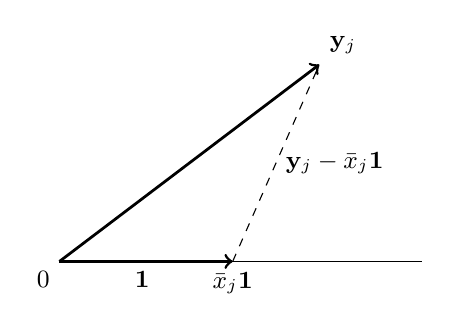
\begin{tikzpicture}[scale=1.0]
\draw (0,0)--(4.6,0);
\draw[->,line width=1.0pt] (0,0)--(3.3,2.5) node[above right,font=\small]{$\mathbf{y}_{j}$};
\draw[->,line width=1.0pt] (0,0)--(2.2,0) node[below,font=\small]{$\bar{x}_{j}\mathbf{1}$};
\draw[dashed] (2.2,0)--(3.3,2.5);
\node[right,font=\small] at (2.75,1.25){$\mathbf{y}_{j}-\bar{x}_{j}\mathbf{1}$};
\node[below left,font=\small] at (0,0){$0$};
\node[below,font=\small] at (1.05,0){$\mathbf{1}$};
\end{tikzpicture}
\end{center}

其中 $\bar{\mathbf{x}}_{j}\mathbf{1}$ 垂直于 $\mathbf{y}_{j}-\bar{x}_{j}\mathbf{1}$. 偏差 (或均值修正) 向量为
\phantomsection\label{eq:3-4}
\begin{equation}
\mathbf{d}_{j}=\mathbf{y}_{j}-\bar{x}_{j}\mathbf{1}=\begin{bmatrix}x_{1j}-\bar{x}_{j}\\x_{2j}-\bar{x}_{j}\\\vdots\\x_{nj}-\bar{x}_{j}\end{bmatrix}
\tag{3-4}
\end{equation}

%% ===== pg-101 =====

$\mathbf{d}_{j}$ 的元素是第 $i$ 个变量的测量值与样本均值的偏差. \hyperref[fig:3.3]{图 3.3} 显示了 $p=3$ 和 $n=3$ 时, $\mathbf{y}_{i}$ 向量分解成均值分量和偏差分量.

\begin{figure}[H]
\centering
\begin{tikzpicture}[scale=0.95]
% 三维斜投影坐标轴
\draw[->] (0,0)--(4.5,0) node[right]{$2$};
\draw[->] (0,0)--(0,3.4) node[above]{$3$};
\draw[->] (0,0)--(-1.9,-1.55) node[below left]{$1$};
\node[font=\scriptsize,below] at (1.6,0){$1$};
\node[font=\scriptsize,below] at (3.4,0){$2$};
\node[font=\scriptsize,left] at (0,1.4){$1$};
\node[font=\scriptsize,left] at (0,2.4){$2$};
\node[font=\scriptsize,above left] at (-1.0,-0.8){$1$};
% 主对角线方向（等角线）
\draw[line width=1.0pt] (0,0)--(1.5,1.15);
% y1 与 d1
\draw[->,line width=1.0pt] (0,0)--(-1.55,-1.25) node[left,font=\small]{$\mathbf{y}_{1}$};
\draw[->,line width=0.9pt] (-1.55,-1.25)--(-0.75,-0.62);
\node[left,font=\scriptsize] at (-1.15,-0.9){$\mathbf{d}_{1}$};
% y2
\draw[->,line width=1.0pt] (2.6,0.35)--(3.15,1.75) node[right,font=\small]{$\mathbf{y}_{2}$};
\node[right,font=\scriptsize] at (0.9,0.72){$\bar{x}_{1}\mathbf{1}$};
\draw[->,line width=0.9pt] (2.55,0.3)--(2.95,1.15);
\node[right,font=\scriptsize] at (2.75,0.65){$\mathbf{d}_{2}$};
% y3
\draw[->,line width=1.0pt] (1.05,0.05)--(1.65,1.35) node[right,font=\small]{$\mathbf{y}_{3}$};
\node[right,font=\scriptsize] at (1.35,-0.05){$\mathbf{d}_{3}$};
\end{tikzpicture}
\phantomsection\label{fig:3.3}\mvcap{图 3.3\quad $\mathbf{y}_{i}$ 分解为一个 $\bar{x}_{i}\mathbf{1}$ 分量和一个偏差分量 $\mathbf{d}_{i}=\mathbf{y}_{i}-\bar{x}_{i}\mathbf{1},i=1,2,3$}
\end{figure}

\medskip
\noindent\textbf{例 3.3}\quad (把一个向量分解成均值分量和偏差分量)

对例 3.2 中所给数据 $\mathbf{X}=\begin{bmatrix}4&1\\-1&3\\3&5\end{bmatrix}$, 把 $\mathbf{y}_{i}$ 分解为 $\bar{x}_{i}\mathbf{1}$ 和 $\mathbf{d}_{i}=\mathbf{y}_{i}-\bar{x}_{i}\mathbf{1},i=1,2$.

这里 $\bar{x}_{1}=(4-1+3)/3=2,\bar{x}_{2}=(1+3+5)/3=3$, 因此,
\[
\bar{x}_{1}\mathbf{1}=2\begin{bmatrix}1\\1\\1\end{bmatrix}=\begin{bmatrix}2\\2\\2\end{bmatrix}\qquad
\bar{x}_{2}\mathbf{1}=3\begin{bmatrix}1\\1\\1\end{bmatrix}=\begin{bmatrix}3\\3\\3\end{bmatrix}
\]
所以,
\[
\mathbf{d}_{1}=\mathbf{y}_{1}-\bar{x}_{1}\mathbf{1}=\begin{bmatrix}4\\-1\\3\end{bmatrix}-\begin{bmatrix}2\\2\\2\end{bmatrix}=\begin{bmatrix}2\\-3\\1\end{bmatrix}
\]
和
\[
\mathbf{d}_{2}=\mathbf{y}_{2}-\bar{x}_{2}\mathbf{1}=\begin{bmatrix}1\\3\\5\end{bmatrix}-\begin{bmatrix}3\\3\\3\end{bmatrix}=\begin{bmatrix}-2\\0\\2\end{bmatrix}
\]
注意, 因为
\[
(\bar{x}_{1}\mathbf{1})'(\mathbf{y}_{1}-\bar{x}_{1}\mathbf{1})=[2\quad2\quad2]\begin{bmatrix}2\\-3\\1\end{bmatrix}=4-6+2=0
\]
所以 $\bar{x}_{1}\mathbf{1}$ 和 $\mathbf{d}_{1}=\mathbf{y}_{1}-\bar{x}_{1}\mathbf{1}$ 是垂直的.

对于 $\bar{x}_{1}\mathbf{1}$ 和 $\mathbf{d}_{2}=\mathbf{y}_{2}-\bar{x}_{2}\mathbf{1}$, 类似的结论成立. 分解式为
\[
\mathbf{y}_{1}=\begin{bmatrix}4\\-1\\3\end{bmatrix}=\begin{bmatrix}2\\2\\2\end{bmatrix}+\begin{bmatrix}2\\-3\\1\end{bmatrix}
\]
\[
\mathbf{y}_{2}=\begin{bmatrix}1\\3\\5\end{bmatrix}=\begin{bmatrix}3\\3\\3\end{bmatrix}+\begin{bmatrix}-2\\0\\2\end{bmatrix}
\]
\hfill$\blacksquare$

%% ===== pg-102 =====

目前我们感兴趣的是偏差 (或剩余) 向量 $\mathbf{d}_{j}=\mathbf{y}_{j}-\bar{x}_{j}\mathbf{1}$. 在图 3.4 中给出了\hyperref[fig:3.3]{图 3.3} 中的偏差向量图. 我们在不改变偏差向量的长度和方向的情况下, 把它们平移到原点.

现在考虑偏差向量的长度的平方. 利用\hyperref[eq:2-5]{式(2-5)} 和\hyperref[eq:3-4]{式(3-4)}, 得到
\phantomsection\label{eq:3-5}
\begin{equation}
L_{\mathbf{d}_{j}}^{2}=\mathbf{d}_{j}'\mathbf{d}_{j}=\sum_{i=1}^{n}(x_{ij}-\bar{x}_{j})^{2}
\tag{3-5}
\end{equation}
(偏差向量长度)$^{2}$ = 偏差的平方和.

从\hyperref[eq:1-3]{式(1-3)} 可见, 长度的平方是与第 $j$ 个变量的测量值的方差成比例的. 等价地, 长度是与标准差成比例的. 较长的向量比较短的向量表现出更多的变化性.

对于任何两个偏差向量 $\mathbf{d}_{j}$ 和 $\mathbf{d}_{k}$,
\phantomsection\label{eq:3-6}
\begin{equation}
\mathbf{d}_{j}'\mathbf{d}_{k}=\sum_{i=1}^{n}(x_{ij}-\bar{x}_{j})(x_{ik}-\bar{x}_{k})
\tag{3-6}
\end{equation}
令 $\theta_{jk}$ 表示向量 $\mathbf{d}_{j}$ 和 $\mathbf{d}_{k}$ 所成的角. 从\hyperref[eq:2-6]{式(2-6)}, 得到
\[
\mathbf{d}_{j}'\mathbf{d}_{k}=L_{\mathbf{d}_{j}}L_{\mathbf{d}_{k}}\cos(\theta_{jk})
\]
或利用\hyperref[eq:3-5]{式(3-5)} 和\hyperref[eq:3-6]{式(3-6)}, 得到
\[
\sum_{i=1}^{n}(x_{ij}-\bar{x}_{j})(x_{ik}-\bar{x}_{k})=\sqrt{\sum_{i=1}^{n}(x_{ij}-\bar{x}_{j})^{2}}\sqrt{\sum_{i=1}^{n}(x_{ik}-\bar{x}_{k})^{2}}\cos(\theta_{jk})
\]
因此 [参见\hyperref[eq:1-5]{式(1-5)}],
\phantomsection\label{eq:3-7}
\begin{equation}
r_{ik}=\frac{s_{ik}}{\sqrt{s_{ii}}\sqrt{s_{kk}}}=\cos(\theta_{jk})
\tag{3-7}
\end{equation}
夹角的余弦是样本相关系数. 若两个偏差向量几乎方向相同, 其样本相关系数将接近于 1. 若两个向量几乎是垂直的, 其样本相关系数将接近零. 若两个向量几乎是相反方向的, 其样本相关系数将接近于 $-1$.

\begin{figure}[H]
\centering
\begin{tikzpicture}[scale=0.85]
\draw[->] (0,0)--(3.6,0) node[right]{$2$};
\draw[->] (0,0)--(0,3.2) node[above]{$3$};
\draw[->] (0,0)--(-1.7,-1.4) node[below left]{$1$};
\draw[->,line width=1.0pt] (0,0)--(1.9,2.1) node[right,font=\small]{$\mathbf{d}_{2}$};
\draw[->,line width=1.0pt] (0,0)--(1.3,-1.05) node[right,font=\small]{$\mathbf{d}_{1}$};
\draw[->,line width=1.0pt] (0,0)--(2.2,-0.35) node[right,font=\small]{$\mathbf{d}_{3}$};
\end{tikzpicture}
\caption{图 3.3 中的偏差向量 $\mathbf{d}_{i}$}
\end{figure}

\medskip
\noindent\textbf{例 3.4}\quad (由偏差向量计算 $\mathbf{S}_{n}$ 和 $\mathbf{R}$)

给定例 3.3 中的偏差向量, 利用刚刚介绍过的几何概念计算样本方差-协方差矩阵 $\mathbf{S}_{n}$ 和样本相关矩阵 $\mathbf{R}$.

\begin{figure}[H]
\centering
\begin{tikzpicture}[scale=0.68]
\draw[->] (-3.4,0)--(4.6,0) node[right]{$x_{1}$};
\draw[->] (0,-2.6)--(0,7.2) node[above]{$x_{2}$};
\foreach \x in {-3,-2,-1,1,2,3,4} \draw (\x,0.08)--(\x,-0.08) node[below,font=\scriptsize]{\x};
\foreach \y in {-2,-1,1,2,3,4,5,6} \draw (0.08,\y)--(-0.08,\y) node[left,font=\scriptsize]{\y};
% d1=(-2,2), d2=(2,0)
\draw[->,line width=1.0pt] (0,0)--(-2,2) node[below left,font=\small]{$\mathbf{d}_{1}$};
\draw[->,line width=1.0pt] (0,0)--(2,0) node[right,font=\small]{$\mathbf{d}_{2}$};
\draw (1.0,0) arc (0:135:1.0);
\node[font=\scriptsize] at (0.95,0.42){$\theta_{12}$};
\end{tikzpicture}
\caption{偏差向量 $\mathbf{d}_{1}$ 和 $\mathbf{d}_{2}$}
\end{figure}

由例 3.3,
\[
\mathbf{d}_{1}=\begin{bmatrix}2\\-3\\1\end{bmatrix}\quad\text{和}\quad \mathbf{d}_{2}=\begin{bmatrix}-2\\0\\2\end{bmatrix}
\]
这两个向量平移到原点后, 如图 3.5 所示. 现在
\[
\mathbf{d}_{1}'\mathbf{d}_{1}=\begin{bmatrix}2&-3&1\end{bmatrix}\begin{bmatrix}2\\-3\\1\end{bmatrix}=14=3s_{11}
\]
即 $s_{11}=14/3$. 又
\[
\mathbf{d}_{2}'\mathbf{d}_{2}=\begin{bmatrix}-2&0&2\end{bmatrix}\begin{bmatrix}-2\\0\\2\end{bmatrix}=8=3s_{22}
\]

%% ===== pg-103 =====

即 $s_{22}=8/3$. 最后,
\[
\mathbf{d}_{1}'\mathbf{d}_{2}=\begin{bmatrix}2&-3&1\end{bmatrix}\begin{bmatrix}-2\\0\\2\end{bmatrix}=-2=3s_{12}
\]
即 $s_{12}=-2/3$. 因此,
\[
r_{12}=\frac{s_{12}}{\sqrt{s_{11}}\sqrt{s_{22}}}=\frac{-\dfrac{2}{3}}{\sqrt{\dfrac{14}{3}}\times\sqrt{\dfrac{8}{3}}}=-0.189
\]
和
\[
\mathbf{S}_{n}=\begin{bmatrix}\dfrac{14}{3}&-\dfrac{2}{3}\\[8pt]-\dfrac{2}{3}&\dfrac{8}{3}\end{bmatrix},\quad
\mathbf{R}=\begin{bmatrix}1&-0.189\\-0.189&1\end{bmatrix}
\]
\hfill$\blacksquare$

长度、角度和投影的概念已经给我们提供了样本的几何解释, 可概述如下:

\begin{mvbox}
\begin{center}
\textbf{样本的几何解释}
\end{center}
1.\quad 数据矩阵 $\mathbf{X}$ 的一列 $\mathbf{y}_{i}$ 在等角向量 $\mathbf{1}$ 上的投影是向量 $\bar{x}_{i}\mathbf{1}$, 向量 $\bar{x}_{i}\mathbf{1}$ 的长度为 $\sqrt{n}\,|\bar{x}_{i}|$. 因此, 第 $i$ 个样本均值 $\bar{x}_{i}$ 与 $\mathbf{y}_{i}$ 在 $\mathbf{1}$ 上的投影的长度有关.

2.\quad 从偏差向量 $\mathbf{d}_{j}=\mathbf{y}_{j}-\bar{x}_{j}\mathbf{1}=[x_{1j}-\bar{x}_{j},x_{2j}-\bar{x}_{j},\cdots,x_{nj}-\bar{x}_{j}]'$ 可得到 $\mathbf{S}_{n}$ 的有关信息. $\mathbf{d}_{j}$ 长度的平方是 $ns_{jj}$, 且 $\mathbf{d}_{j}$ 和 $\mathbf{d}_{k}$ 的 (内) 积是 $ns_{jk}$. \footnote{{\footnotesize 当因子 $n-1$ 用于样本方差和协方差的定义中时, 长度的平方以及内积分别是 $(n-1)s_{jj}$ 和 $(n-1)s_{jk}$.}}

3.\quad 样本相关系数 $r_{jk}$ 是 $\mathbf{d}_{j}$ 和 $\mathbf{d}_{k}$ 之间夹角的余弦.
\end{mvbox}

\section{随机样本以及样本均值和协方差矩阵的期望值}
\phantomsection\label{sec:3.3}

为了研究诸如 $\bar{\mathbf{x}}$ 和 $\mathbf{S}_{n}$ 等统计量的抽样变异性, 以便最终作出推断, 我们必须对其观测值构成数据 $\mathbf{X}$ 的变量作出假设.

假定, 数据还没有观测, 但我们想要对 $p$ 个变量收集 $n$ 组测量结果. 在测量之前, 通常不能准确地预计它们的值. 因此, 把它们当做随机变量来处理. 本书中令数据矩阵中第 $(j,k)$ 个元素代表随机变量 $X_{jk}$ 的 $p$ 个变量的每组测量结果 $\mathbf{X}_{j}$, 是一个随机向量, 且有随机矩阵
\phantomsection\label{eq:3-8}
\begin{equation}
\mathbf{X}=\begin{bmatrix}
X_{11}&X_{12}&\cdots&X_{1p}\\
X_{21}&X_{22}&\cdots&X_{2p}\\
\vdots&\vdots&&\vdots\\
X_{n1}&X_{n2}&\cdots&X_{np}
\end{bmatrix}
=\begin{bmatrix}\mathbf{X}_{1}'\\\mathbf{X}_{2}'\\\vdots\\\mathbf{X}_{n}'\end{bmatrix}
\tag{3-8}
\end{equation}
现在就来定义随机样本.

如果\hyperref[eq:3-8]{式(3-8)} 中的行向量 $\mathbf{X}_{1}',\mathbf{X}_{2}',\cdots,\mathbf{X}_{n}'$ 代表来自密度函数为 $f(\mathbf{x})=f(x_{1},x_{2},\cdots,x_{p})$ 的一个公共联合分布的独立观测值, 则称 $\mathbf{X}_{1},\mathbf{X}_{2},\cdots,\mathbf{X}_{n}$ 构成一个来自 $f(\mathbf{x})$ 的随机样本. 在数学上, 若 $\mathbf{X}_{1},\mathbf{X}_{2},\cdots,\mathbf{X}_{n}$ 的联合密度函数由乘积 $f(\mathbf{x}_{1})f(\mathbf{x}_{2})\cdots f(\mathbf{x}_{n})$ 给出, 其中 $f(\mathbf{x}_{j})=f(x_{j1},x_{j2},\cdots,x_{jp})$ 是第 $j$ 个行向量的密度函数, 则称它们构成一个随机样本.

%% ===== pg-104 =====

对随机样本的定义有两点特别值得注意:

1.\quad 在单个试验中, $p$ 个变量的测量结果, 例如 $\mathbf{X}_{j}'=[X_{j1},X_{j2},\cdots,X_{jp}]$, 常常是相关的. 的确, 我们期望这是事实. 然而, 从不同试验得到的测量结果必须是独立的.

2.\quad 当变量可能会随时间缓慢地变化时, 例如 $p$ 种股票价格或 $p$ 个经济指标构成的集合, 各次试验的测量结果的独立性可能不成立. 违背独立性的临时假设对统计推断的性质会有严重影响.

下列例子将说明这些道理.

\medskip
\noindent\textbf{例 3.5}\quad (选择一个随机样本)

为了设计一种准入制度使野外划舟区不至于太拥挤, 一位自然资源经理首先对客户进行了调查. 整个野外区域被分成许多子区域, 并要求应答者给出有关访问区域、逗留时间及其他变量的信息.

接下来的办法是, 在特定一周内对进入该野外区域的所有人进行随机抽选 (可以利用随机数表). 所有人员以等可能的机会被选为样本, 因此, 划舟者的比例越大表示进入此区域的人越多.

这里, 我们会期望样本观测值严格符合用户或潜在用户总体的随机样本的标准. 另一方面, 如果一个取样者等待在深入区域内部的营地, 并仅调查到达该地的划舟者, 那么相继的观测结果不会是独立的. 例如, 停留时间会趋向于较长.\hfill$\blacksquare$

\medskip
\noindent\textbf{例 3.6}\quad (非随机样本)

由于关注未来如何对固体废品进行处理, 因而对美国每年产生的固体废品的总重量进行了研究 (环境保护署). \hyperref[tab:3.1]{表 3.1} 给出了所选年份中 $x_{1}=$ 废纸及废记录纸和 $x_{2}=$ 塑料废品 (按百万吨计算) 的估计总量. $\mathbf{X}'=[X_{1},X_{2}]$ 中的这些观测结果可否作为一个 $n=7$ 的随机样本来处理? 不! 其实除了在 2003 年的废纸及废纸板数据略有下降外, 这两个变量是随时间而增加的. 各年的值是来自同一分布的独立观测值, 这种情况是很少的.

\begin{mvtable}
\phantomsection\label{tab:3.1}\mvtabcap{表 3.1\quad 固体废品}
\centering
\begin{tabular}{lccccccc}
\toprule
年 & 1960 & 1970 & 1980 & 1990 & 1995 & 2000 & 2003\\
\midrule
$x_{1}$(纸) & 29.2 & 44.3 & 55.2 & 72.7 & 81.7 & 87.7 & 83.1\\
$x_{2}$(塑料) & 0.4 & 2.9 & 6.8 & 17.1 & 18.9 & 24.7 & 26.7\\
\bottomrule
\end{tabular}
\end{mvtable}

在第 1 章中, 我们初步讨论过, 统计独立的概念对测量距离有重要的意义. 若向量的分量之间是独立的并有相同的方差, 欧几里得距离是合适的. 假定我们考虑作为 $n$ 维空间中一点 $\mathbf{X}$ 的第 $k$ 列 $\mathbf{Y}_{k}=[X_{1k},X_{2k},\cdots,X_{nk}]$ 的位置. 该点的位置是由联合分布 $f(\mathbf{y}_{k})=f(x_{1k},x_{2k},\cdots,x_{nk})$ 确定的. 当测量结果 $X_{1k},X_{2k},\cdots,X_{nk}$ 是一随机样本时, $f(\mathbf{y}_{k})=f(x_{1k},x_{2k},\cdots,x_{nk})=f_{k}(x_{1k})f_{k}(x_{2k})\cdots f_{k}(x_{nk})$. 因此, 每个坐标 $x_{ik}$ 通过相同的边缘分布 $f_{k}(x_{jk})$ 同等地影响着位置.

若 $n$ 个分量不是独立的或边缘分布是不相同的, 单个的观测结果 (坐标) 对位置的影响是不对称的. 因此, 应考虑一个距离函数, 其中不同的坐标将不等地加权, 如同第 1 和第 2 章中介绍的“统计”距离或二次型.

在不对变量的基本联合分布的形式作更多假定的情况下, 可以得到关于 $\bar{\mathbf{x}}$ 和 $\mathbf{S}_{n}$ 的抽样分布的某些结论. 具体地说, 我们可以看到 $\bar{\mathbf{x}}$ 和 $\mathbf{S}_{n}$ 如何作为相应的总体均值向量 $\boldsymbol{\mu}$ 和协方差矩阵 $\boldsymbol{\Sigma}$ 的点估计.

%% ===== pg-105 =====

\mvthm{结论 3.1}{设 $\mathbf{X}_{1},\mathbf{X}_{2},\cdots,\mathbf{X}_{n}$ 是来自均值向量为 $\boldsymbol{\mu}$, 协方差矩阵为 $\boldsymbol{\Sigma}$ 的联合分布的一个随机样本, 则 $\bar{\mathbf{X}}$ 是 $\boldsymbol{\mu}$ 的一个无偏估计量, 它的协方差矩阵是 $\dfrac{1}{n}\boldsymbol{\Sigma}$}

即
\phantomsection\label{eq:3-9}
\begin{equation}
\begin{aligned}
E(\bar{\mathbf{X}})&=\boldsymbol{\mu}\qquad(\text{总体均值向量})\\[4pt]
\operatorname{Cov}(\bar{\mathbf{X}})&=\frac{1}{n}\boldsymbol{\Sigma}\qquad(\text{总体方差-协方差矩阵除以样本大小})
\end{aligned}
\tag{3-9}
\end{equation}
对协方差矩阵 $\mathbf{S}_{n}$,
\[
E(\mathbf{S}_{n})=\frac{n-1}{n}\boldsymbol{\Sigma}=\boldsymbol{\Sigma}-\frac{1}{n}\boldsymbol{\Sigma}
\]
因此,
\phantomsection\label{eq:3-10}
\begin{equation}
E\Bigl(\frac{n}{n-1}\mathbf{S}_{n}\Bigr)=\boldsymbol{\Sigma}
\tag{3-10}
\end{equation}
所以 $[n/(n-1)]\mathbf{S}_{n}$ 是 $\boldsymbol{\Sigma}$ 的无偏估计量, 而 $\mathbf{S}_{n}$ 是有偏估计量, 偏差 $=E(\mathbf{S}_{n})-\boldsymbol{\Sigma}=-(1/n)\boldsymbol{\Sigma}$.

\medskip
\noindent\mvbold{证明}\quad 现在, $\bar{\mathbf{X}}=(\mathbf{X}_{1}+\mathbf{X}_{2}+\cdots+\mathbf{X}_{n})/n$, 对两个向量重复利用\hyperref[eq:2-24]{式(2-24)} 中期望的性质, 得出
\begin{align*}
E(\bar{\mathbf{X}})&=E\Bigl(\frac{1}{n}\mathbf{X}_{1}+\frac{1}{n}\mathbf{X}_{2}+\cdots+\frac{1}{n}\mathbf{X}_{n}\Bigr)\\
&=E\Bigl(\frac{1}{n}\mathbf{X}_{1}\Bigr)+E\Bigl(\frac{1}{n}\mathbf{X}_{2}\Bigr)+\cdots+E\Bigl(\frac{1}{n}\mathbf{X}_{n}\Bigr)\\
&=\frac{1}{n}E(\mathbf{X}_{1})+\frac{1}{n}E(\mathbf{X}_{2})+\cdots+\frac{1}{n}E(\mathbf{X}_{n})=\frac{1}{n}\boldsymbol{\mu}+\frac{1}{n}\boldsymbol{\mu}+\cdots+\frac{1}{n}\boldsymbol{\mu}\\
&=\boldsymbol{\mu}
\end{align*}
接下来,
\begin{align*}
(\bar{\mathbf{X}}-\boldsymbol{\mu})(\bar{\mathbf{X}}-\boldsymbol{\mu})'
&=\Bigl(\frac{1}{n}\sum_{l=1}^{n}(\mathbf{X}_{l}-\boldsymbol{\mu})\Bigr)\Bigl(\frac{1}{n}\sum_{l=1}^{n}(\mathbf{X}_{l}-\boldsymbol{\mu})\Bigr)'\\
&=\frac{1}{n^{2}}\sum_{l=1}^{n}\sum_{l'=1}^{n}(\mathbf{X}_{l}-\boldsymbol{\mu})(\mathbf{X}_{l'}-\boldsymbol{\mu})'
\end{align*}
因此,
\[
\operatorname{Cov}(\bar{\mathbf{X}})=E(\bar{\mathbf{X}}-\boldsymbol{\mu})(\bar{\mathbf{X}}-\boldsymbol{\mu})'
=\frac{1}{n^{2}}\Bigl(\sum_{l=1}^{n}\sum_{l'=1}^{n}E(\mathbf{X}_{l}-\boldsymbol{\mu})(\mathbf{X}_{l'}-\boldsymbol{\mu})'\Bigr)
\]
对于 $j\ne l$, 由于 $\mathbf{X}_{j}$ 的分量与 $\mathbf{X}_{l}$ 的分量之间是相互独立的, 其间的协方差是零, 所以 $E(\mathbf{X}_{l}-\boldsymbol{\mu})(\mathbf{X}_{l'}-\boldsymbol{\mu})'$ 中的每一项都是零 [参考练习 3.17 和\hyperref[eq:2-29]{式(2-29)}].

因此,
\[
\operatorname{Cov}(\bar{\mathbf{X}})=\frac{1}{n^{2}}\Bigl(\sum_{l=1}^{n}E(\mathbf{X}_{l}-\boldsymbol{\mu})(\mathbf{X}_{l}-\boldsymbol{\mu})'\Bigr)
\]
由于 $\boldsymbol{\Sigma}=E(\mathbf{X}_{l}-\boldsymbol{\mu})(\mathbf{X}_{l}-\boldsymbol{\mu})'$ 为每个 $\mathbf{X}_{l}$ 的共同的总体协方差矩阵, 我们有
\begin{align*}
\operatorname{Cov}(\bar{\mathbf{X}})&=\frac{1}{n^{2}}\Bigl(\sum_{l=1}^{n}E(\mathbf{X}_{l}-\boldsymbol{\mu})(\mathbf{X}_{l}-\boldsymbol{\mu})'\Bigr)
=\frac{1}{n^{2}}(\underbrace{\boldsymbol{\Sigma}+\boldsymbol{\Sigma}+\cdots+\boldsymbol{\Sigma}}_{n\ \text{个}})\\
&=\frac{1}{n^{2}}(n\boldsymbol{\Sigma})=\Bigl(\frac{1}{n}\Bigr)\boldsymbol{\Sigma}
\end{align*}

%% ===== pg-106 =====

为了得到 $\mathbf{S}_{n}$ 的期望值, 首先注意到 $(X_{il}-\bar{X}_{i})(X_{kl}-\bar{X}_{k})$ 是 $(\mathbf{X}_{l}-\bar{\mathbf{X}})(\mathbf{X}_{l}-\bar{\mathbf{X}})'$ 的第 $(i,k)$ 个元素. 由于 $\sum_{l=1}^{n}(\mathbf{X}_{l}-\bar{\mathbf{X}})=\mathbf{0}$ 和 $n\bar{\mathbf{X}}'=\sum_{l=1}^{n}\mathbf{X}_{l}'$, 代表平方和与交叉乘积的矩阵可以写做
\begin{align*}
\sum_{l=1}^{n}(\mathbf{X}_{l}-\bar{\mathbf{X}})(\mathbf{X}_{l}-\bar{\mathbf{X}})'
&=\sum_{l=1}^{n}(\mathbf{X}_{l}-\bar{\mathbf{X}})\mathbf{X}_{l}'+\Bigl(\sum_{l=1}^{n}(\mathbf{X}_{l}-\bar{\mathbf{X}})\Bigr)(-\bar{\mathbf{X}})'\\
&=\sum_{l=1}^{n}\mathbf{X}_{l}\mathbf{X}_{l}'-n\bar{\mathbf{X}}\bar{\mathbf{X}}'
\end{align*}
因此, 它的期望值是
\[
E\Bigl(\sum_{l=1}^{n}\mathbf{X}_{l}\mathbf{X}_{l}'-n\bar{\mathbf{X}}\bar{\mathbf{X}}'\Bigr)=\sum_{l=1}^{n}E(\mathbf{X}_{l}\mathbf{X}_{l}')-nE(\bar{\mathbf{X}}\bar{\mathbf{X}}')
\]
对任何随机向量 $\mathbf{V}$, $E(\mathbf{V})=\boldsymbol{\mu}_{V}$ 和 $\operatorname{Cov}(\mathbf{V})=\boldsymbol{\Sigma}_{V}$, 我们有 $E(\mathbf{V}\mathbf{V}')=\boldsymbol{\Sigma}_{V}+\boldsymbol{\mu}_{V}\boldsymbol{\mu}_{V}'$ (参考练习 3.16). 因此,
\[
E(\mathbf{X}_{l}\mathbf{X}_{l}')=\boldsymbol{\Sigma}+\boldsymbol{\mu}\boldsymbol{\mu}'\quad\text{和}\quad
E(\bar{\mathbf{X}}\bar{\mathbf{X}}')=\frac{1}{n}\boldsymbol{\Sigma}+\boldsymbol{\mu}\boldsymbol{\mu}'
\]
利用这些结论, 我们得到
\[
\sum_{l=1}^{n}E(\mathbf{X}_{l}\mathbf{X}_{l}')-nE(\bar{\mathbf{X}}\bar{\mathbf{X}}')
=n\boldsymbol{\Sigma}+n\boldsymbol{\mu}\boldsymbol{\mu}'-n\Bigl(\frac{1}{n}\boldsymbol{\Sigma}+\boldsymbol{\mu}\boldsymbol{\mu}'\Bigr)=(n-1)\boldsymbol{\Sigma}
\]
又因为 $\mathbf{S}_{n}=(1/n)\Bigl(\sum_{l=1}^{n}\mathbf{X}_{l}\mathbf{X}_{l}'-n\bar{\mathbf{X}}\bar{\mathbf{X}}'\Bigr)$, 因此立即得到
\[
E(\mathbf{S}_{n})=\frac{(n-1)}{n}\boldsymbol{\Sigma}
\]
\hfill$\blacksquare$

结论 3.1 指出, $[n/(n-1)]\mathbf{S}_{n}$ 的第 $(i,k)$ 项 $(n-1)^{-1}\sum_{l=1}^{n}(X_{il}-\bar{X}_{i})(X_{kl}-\bar{X}_{k})$ 是 $\sigma_{ik}$ 的一个无偏估计量. 然而, 无论是用 $n$ 或用 $n-1$ 作除数计算得到的单个的样本标准差 $\sqrt{s_{ii}}$ 都不是对应的总体量 $\sqrt{\sigma_{ii}}$ 的无偏估计量. 而且, 相关系数 $r_{ik}$ 不是总体量 $\rho_{ik}$ 的无偏估计量. 不过, 若样本容量 $n$ 适当大, 偏差 $E(\sqrt{s_{ii}})-\sqrt{\sigma_{ii}}$ 或 $E(r_{ik})-\rho_{ik}$ 通常是可以忽略.

考虑偏差后, 对样本方差-协方差矩阵定义需要进行一个微小的修改. 结论 3.1 提供了 $\boldsymbol{\Sigma}$ 的无偏估计量 $\mathbf{S}$:

\begin{mvbox}
\begin{center}
\mvbold{(无偏) 样本方差-协方差矩阵}
\end{center}
\phantomsection\label{eq:3-11}
\begin{equation}
\mathbf{S}=\Bigl(\frac{n}{n-1}\Bigr)\mathbf{S}_{n}=\frac{1}{n-1}\sum_{l=1}^{n}(\mathbf{X}_{l}-\bar{\mathbf{X}})(\mathbf{X}_{l}-\bar{\mathbf{X}})'
\tag{3-11}
\end{equation}
\end{mvbox}

此处 $\mathbf{S}$ 没有下标, 其第 $(i,k)$ 项为 $(n-1)^{-1}\sum_{l=1}^{n}(X_{il}-\bar{X}_{i})(X_{kl}-\bar{X}_{k})$. 样本协方差的这一定义在许多多元检验统计中被普遍使用. 因此, 在本书后面的许多地方, $\mathbf{S}$ 将取代 $\mathbf{S}_{n}$ 作为样本协方差矩阵.

\section{广义方差}
\phantomsection\label{sec:3.4}

在单变量情形下, 样本方差通常用来描述该变量的观测值变差的程度. 当在每组观测到 $p$ 个变量时, 变差是用样本方差-协方差矩阵来描述.

%% ===== pg-107 =====

\[
\mathbf{S}=\begin{bmatrix}
s_{11}&s_{12}&\cdots&s_{1p}\\
s_{12}&s_{22}&\cdots&s_{2p}\\
\vdots&\vdots&\ddots&\vdots\\
s_{1p}&s_{2p}&\cdots&s_{pp}
\end{bmatrix}
=\Bigl\{s_{ik}=\frac{1}{n-1}\sum_{j=1}^{n}(x_{ji}-\bar{x}_{i})(x_{jk}-\bar{x}_{k})\Bigr\}
\]
该样本协方差矩阵包含 $p$ 个方差和 $\dfrac{1}{2}p(p-1)$ 个可能的不同的协方差. 有时, 希望对用 $\mathbf{S}$ 表示的变差能给定一数值. 我们选择这一数值为 $\mathbf{S}$ 的行列式, 当 $p=1$ 时它就是单一特征的一般样本方差. 该行列式\footnote{{\footnotesize 补充 2A.24 定义了“行列式”, 并指明了计算行列式的值的方法.}}称为广义样本方差.

\begin{mvbox}
\centering
\mvbold{广义样本方差} $=|\mathbf{S}|$ \hspace{3em} (3-12)
\end{mvbox}

\medskip
\noindent\textbf{例 3.7}\quad (计算广义方差)

美国 16 家最大的出版公司的雇员 $(x_{1})$ 和雇员人均利润 $(x_{2})$ 由\hyperref[fig:1.3]{图 1.3} 给出. 从 1990 年 4 月 30 日《福布斯》中的数据得到的样本协方差矩阵为
\[
\mathbf{S}=\begin{bmatrix}252.04&-68.43\\-68.43&123.67\end{bmatrix}
\]
求广义方差的值.

这时, 我们计算
\[
|\mathbf{S}|=252.04\times123.67-(-68.43)\times(-68.43)=26\,487
\]
\hfill$\blacksquare$

广义样本方差提供一种方法, 把所有方差和协方差的信息写成单个的数值. 当然, 在 $p>1$ 时, 用这一方法会丢失样本的某些信息. $|\mathbf{S}|$ 的几何解释将帮助我们了解它作为一个描述性的概括量所具有的优点和缺点.

考虑由两个偏差向量 $\mathbf{d}_{1}=\mathbf{y}_{1}-\bar{x}_{1}\mathbf{1}$ 和 $\mathbf{d}_{2}=\mathbf{y}_{2}-\bar{x}_{2}\mathbf{1}$ 在平面内生成的一个区域. 令 $L_{\mathbf{d}_{1}}$ 是 $\mathbf{d}_{1}$ 的长度, $L_{\mathbf{d}_{2}}$ 是 $\mathbf{d}_{2}$ 的长度, 由初等几何学, 有图

\begin{center}
\begin{tikzpicture}[scale=0.92]
\coordinate (O) at (0,0);
\coordinate (D1) at (1.6,2.1);
\coordinate (D2) at (4.2,0.5);
\coordinate (C) at (5.8,2.6);
\draw[->,line width=1.0pt] (O)--(D1) node[above left,font=\small]{$\mathbf{d}_{1}$};
\draw[->,line width=1.0pt] (O)--(D2) node[below right,font=\small]{$\mathbf{d}_{2}$};
\draw[dashed] (D1)--(C);
\draw[dashed] (D2)--(C);
% 垂线（高）
\draw[dashed] (D1)--(1.913,0.228);
\node[right,font=\scriptsize] at (1.72,1.25){高$=L_{\mathbf{d}_{1}}\sin(\theta)$};
% 角
\draw (0.85,0) arc (0:52.7:0.85);
\node[font=\scriptsize] at (1.02,0.36){$\theta$};
% 长度标注
\node[font=\scriptsize,left] at (0.62,1.15){$L_{\mathbf{d}_{1}}$};
\node[font=\scriptsize,above] at (2.35,0.15){$L_{\mathbf{d}_{2}}$};
\node[font=\scriptsize,above right] at (5.35,2.72){$L_{\mathbf{d}_{2}}$};
\end{tikzpicture}
\end{center}

且此平行四边形的面积是 $|L_{\mathbf{d}_{1}}\sin(\theta)|L_{\mathbf{d}_{2}}$. 由 $\cos^{2}(\theta)+\sin^{2}(\theta)=1$, 此面积可表示为
\[
\text{面积}=L_{\mathbf{d}_{1}}L_{\mathbf{d}_{2}}\sqrt{1-\cos^{2}(\theta)}
\]
由\hyperref[eq:3-5]{式(3-5)} 和\hyperref[eq:3-7]{式(3-7)},
\[
L_{\mathbf{d}_{1}}=\sqrt{\sum_{j=1}^{n}(x_{j1}-\bar{x}_{1})^{2}}=\sqrt{(n-1)s_{11}}
\]
\[
L_{\mathbf{d}_{2}}=\sqrt{\sum_{j=1}^{n}(x_{j2}-\bar{x}_{2})^{2}}=\sqrt{(n-1)s_{22}}
\]
和
\[
\cos(\theta)=r_{12}
\]
因此,

%% ===== pg-108 =====

\phantomsection\label{eq:3-13}
\begin{equation}
\text{面积}=(n-1)\sqrt{s_{11}}\sqrt{s_{22}}\sqrt{1-r_{12}^{2}}=(n-1)\sqrt{s_{11}s_{22}(1-r_{12}^{2})}
\tag{3-13}
\end{equation}
又
\phantomsection\label{eq:3-14}
\begin{equation}
\begin{aligned}
|\mathbf{S}|&=\begin{vmatrix}s_{11}&s_{12}\\s_{12}&s_{22}\end{vmatrix}
=\begin{vmatrix}s_{11}&\sqrt{s_{11}}\sqrt{s_{22}}r_{12}\\[4pt]\sqrt{s_{11}}\sqrt{s_{22}}r_{12}&s_{22}\end{vmatrix}\\[6pt]
&=s_{11}s_{22}-s_{11}s_{22}r_{12}^{2}=s_{11}s_{22}(1-r_{12}^{2})
\end{aligned}
\tag{3-14}
\end{equation}
如果我们比较\hyperref[eq:3-14]{式(3-14)} 和\hyperref[eq:3-13]{式(3-13)}, 可见
\[
|\mathbf{S}|=(\text{面积})^{2}/(n-1)^{2}
\]
对于由 $p-1$ 个偏差向量 $\mathbf{d}_{1},\mathbf{d}_{2},\cdots,\mathbf{d}_{p-1}$ 所产生的 $n$ 维空间的体积, 假定 $|\mathbf{S}|=(n-1)^{-(p-1)}(\text{体积})^{2}$ 成立, 那么, 对于 $p$ 个偏差向量, 由归纳法, 我们可以确定以下一般性的结论 (参见文献 [1]):
\phantomsection\label{eq:3-15}
\begin{equation}
\text{广义样本方差}=|\mathbf{S}|=(n-1)^{-p}(\text{体积})^{2}
\tag{3-15}
\end{equation}
\hyperref[eq:3-15]{式(3-15)} 说明, 对于一个固定的数据集合, 广义样本方差是与由 $p$ 个偏差向量\footnote{如果广义方差是用样本协方差矩阵 $\mathbf{S}_{n}=[(n-1)/n]\mathbf{S}$ 定义, 则利用结论 2A.11, $|\mathbf{S}_{n}|=|[(n-1)/n]\mathbf{I}_{p}||\mathbf{S}|=[(n-1)/n]^{p}|\mathbf{I}_{p}||\mathbf{S}|=[(n-1)/n]^{p}|\mathbf{S}|$. 因此, 利用\hyperref[eq:3-15]{式(3-15)}, 我们也可以有: 广义样本方差 $=|\mathbf{S}_{n}|=n^{-p}(\text{体积})^{2}$.} $\mathbf{d}_{1}=\mathbf{y}_{1}-\bar{x}_{1}\mathbf{1}$, $\mathbf{d}_{2}=\mathbf{y}_{2}-\bar{x}_{2}\mathbf{1},\cdots,\mathbf{d}_{p}=\mathbf{y}_{p}-\bar{x}_{p}\mathbf{1}$ 生成的体积的平方成比例的. \hyperref[fig:3.6]{图 3.6}(a) 和 (b) 指出了由 $p=3$ 所对应的“大的”和“小的”广义方差的剩余向量生成的梯形区域.

\begin{center}
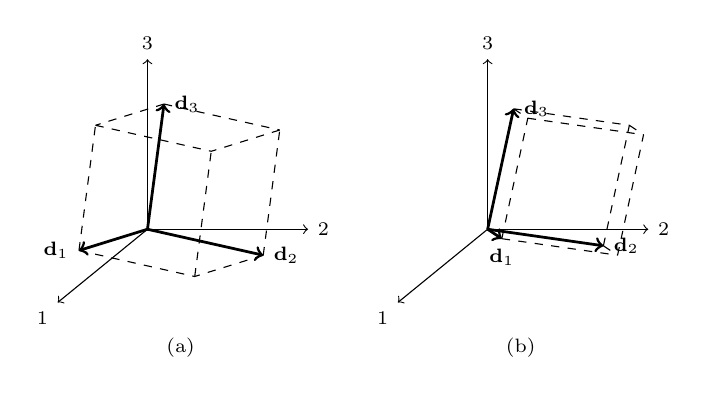
\begin{tikzpicture}[scale=0.60]
% ===== (a) 大的广义样本方差 =====
\begin{scope}
\draw[->] (0,0)--(3.4,0) node[right,font=\scriptsize]{$2$};
\draw[->] (0,0)--(0,3.6) node[above,font=\scriptsize]{$3$};
\draw[->] (0,0)--(-1.9,-1.55) node[below left,font=\scriptsize]{$1$};
\coordinate (O) at (0,0);
\coordinate (A) at (-1.45,-0.45);
\coordinate (B) at (2.45,-0.55);
\coordinate (C) at (0.35,2.65);
\coordinate (D) at (1.00,-1.00);
\coordinate (E) at (-1.10,2.20);
\coordinate (F) at (2.80,2.10);
\coordinate (G) at (1.35,1.65);
\draw[->,line width=1.0pt] (O)--(A) node[left,font=\scriptsize]{$\mathbf{d}_{1}$};
\draw[->,line width=1.0pt] (O)--(B) node[right,font=\scriptsize]{$\mathbf{d}_{2}$};
\draw[->,line width=1.0pt] (O)--(C) node[right,font=\scriptsize]{$\mathbf{d}_{3}$};
\draw[dashed] (A)--(D) (B)--(D) (A)--(E) (C)--(E) (B)--(F) (C)--(F) (D)--(G) (E)--(G) (F)--(G);
\node[font=\scriptsize] at (0.7,-2.5){(a)};
\end{scope}
% ===== (b) 小的广义样本方差 =====
\begin{scope}[shift={(7.2,0)}]
\draw[->] (0,0)--(3.4,0) node[right,font=\scriptsize]{$2$};
\draw[->] (0,0)--(0,3.6) node[above,font=\scriptsize]{$3$};
\draw[->] (0,0)--(-1.9,-1.55) node[below left,font=\scriptsize]{$1$};
\coordinate (O2) at (0,0);
\coordinate (A2) at (0.55,2.55);
\coordinate (B2) at (2.45,-0.35);
\coordinate (C2) at (0.30,-0.20);
\coordinate (D2) at (3.00,2.20);
\coordinate (E2) at (0.85,2.35);
\coordinate (F2) at (2.75,-0.55);
\coordinate (G2) at (3.30,2.00);
\draw[->,line width=1.0pt] (O2)--(A2) node[right,font=\scriptsize]{$\mathbf{d}_{3}$};
\draw[->,line width=1.0pt] (O2)--(B2) node[right,font=\scriptsize]{$\mathbf{d}_{2}$};
\draw[->,line width=1.0pt] (O2)--(C2) node[below,font=\scriptsize]{$\mathbf{d}_{1}$};
\draw[dashed] (A2)--(E2) (C2)--(E2) (B2)--(F2) (C2)--(F2) (A2)--(D2) (B2)--(D2) (E2)--(G2) (F2)--(G2) (D2)--(G2);
\node[font=\scriptsize] at (0.7,-2.5){(b)};
\end{scope}
\end{tikzpicture}
\end{center}

\begin{center}
\phantomsection\label{fig:3.6}{\zihao{6}\heiti 图 3.6}\\[2pt]
{\zihao{6} (a) 对 $p=3$, “大的”广义样本方差}\\[2pt]
{\zihao{6} (b) 对 $p=3$, “小的”广义样本方差}
\end{center}

对于一个固定大小的样本, 根据几何学, 当任何 $\mathbf{d}_{i}=\mathbf{y}_{i}-\bar{x}_{i}\mathbf{1}$ (或 $\sqrt{s_{ii}}$) 的长度增加时, 明显地体积或 $|\mathbf{S}|$ 也增加. 另外, 如果移动固定长度的剩余向量直到它们互相成直角为止时, 体积也将增加, 如\hyperref[fig:3.6]{图 3.6}(a). 另一方面, 如果仅仅 $s_{ii}$ 的一个是小的, 或者偏差向量之一几乎在由其他向量或两个向量构成的 (超) 平面中时, 体积或 $|\mathbf{S}|$ 将是小的. 在第二种情况中, 不规则四边形在平面上有很小的高. 这情况如\hyperref[fig:3.6]{图 3.6}(b) 所示, 其中 $\mathbf{d}_{1}$ 几乎在由 $\mathbf{d}_{2}$ 和 $\mathbf{d}_{3}$ 所构成的平面内.

在 $p$ 维空间广义方差也有解释, 即数据的散布图表示法. 大多数直观的解释涉及关于样

%% ===== pg-109 =====

本均值点 $\bar{\mathbf{x}}'=(\bar{x}_{1},\bar{x}_{2},\cdots,\bar{x}_{p})$ 的散布范围. 考虑在\hyperref[eq:2-19]{式(2-19)} 下面的评注中所给出的距离的测度, $\bar{\mathbf{x}}$ 起不变的点的作用, $\mathbf{S}^{-1}$ 起 $\mathbf{A}$ 的作用. 作出选择后, 距 $\bar{\mathbf{x}}$ 为常数距离 $c$ 的点的坐标 $\mathbf{x}'=[x_{1},x_{2},\cdots,x_{p}]$ 满足
\phantomsection\label{eq:3-16}
\begin{equation}
(\mathbf{x}-\bar{\mathbf{x}})'\mathbf{S}^{-1}(\mathbf{x}-\bar{\mathbf{x}})=c^{2}
\tag{3-16}
\end{equation}
(当 $p=1$ 时, $(\mathbf{x}-\bar{\mathbf{x}})'\mathbf{S}^{-1}(\mathbf{x}-\bar{\mathbf{x}})=(x_{1}-\bar{x}_{1})^{2}/s_{11}$ 是从 $\bar{x}_{1}$ 到 $x_{1}$ 的单位标准差的距离平方.)

\hyperref[eq:3-16]{式(3-16)} 定义一个中心在 $\bar{\mathbf{x}}$ 的超椭球 (如果 $p=2$, 则为椭圆). 可以利用积分计算证明这个超椭球的体积与 $|\mathbf{S}|$ 有关, 具体的,
\phantomsection\label{eq:3-17}
\begin{equation}
\{\mathbf{x}:(\mathbf{x}-\bar{\mathbf{x}})'\mathbf{S}^{-1}(\mathbf{x}-\bar{\mathbf{x}})\le c^{2}\}\ \text{的体积}=k_{p}|\mathbf{S}|^{1/2}c^{p}
\tag{3-17}
\end{equation}
或
\[
(\text{椭球的体积})^{2}=(\text{常数})\times(\text{广义样本方差})
\]
其中常数 $k_{p}$ 很难计算.\footnote{{\footnotesize 对那些好奇的人, 我们给出 $k_{p}=2\pi^{p/2}/p\Gamma(p/2)$, 其中 $\Gamma(z)$ 是在 $z$ 处的伽马函数值.}} 一个大的体积对应于一个大的广义方差.

虽然广义方差有一些直观合意的几何解释, 作为样本协方差矩阵 $\mathbf{S}$ 的一个描述性概括量, 它有一个基本缺点, 如下例所示.

\medskip
\noindent\textbf{例 3.8}\quad (解释广义方差)

\hyperref[fig:3.7]{图 3.7} 给出三个相关模式很不同的散布图. 全部三个数据集有 $\bar{\mathbf{x}}'=[1,2]$ 且协方差矩阵是
\[
\mathbf{S}=\begin{bmatrix}5&4\\4&5\end{bmatrix},\ r=0.8\qquad
\mathbf{S}=\begin{bmatrix}3&0\\0&3\end{bmatrix},\ r=0\qquad
\mathbf{S}=\begin{bmatrix}5&-4\\-4&5\end{bmatrix},\ r=-0.8
\]

\begin{mvfigure}
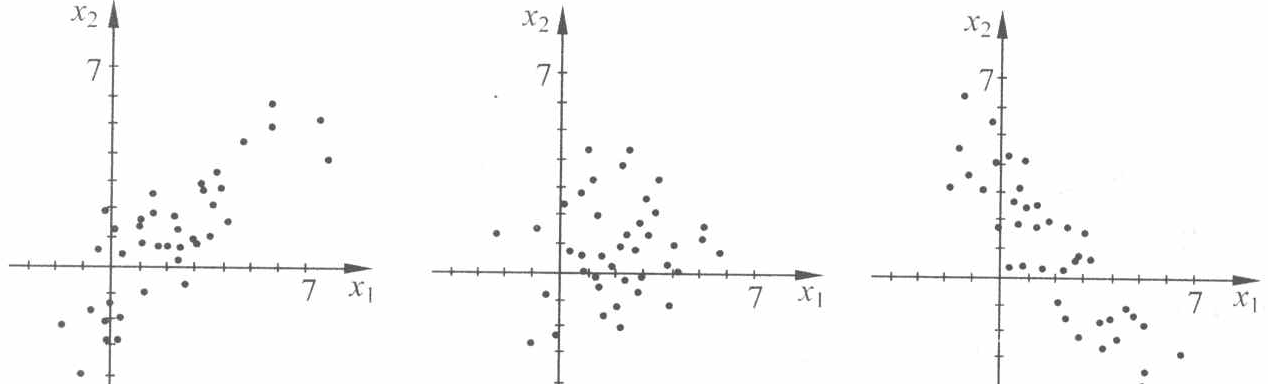
\includegraphics[width=107.3mm]{figs/fig_pg109_1.png}
\phantomsection\label{fig:3.7}\mvcap{图 3.7\quad 三个不同定向的散布图}
\end{mvfigure}

每个协方差矩阵 $\mathbf{S}$ 含有关于变量分量的可变性的信息, 还含有计算相关系数所需的信息. 在这个意义上, $\mathbf{S}$ 刻画了散布图的定向和大小.

从 $\mathbf{S}$ 计算出的特征值和特征向量可更进一步描述散布图中的模型. 对于
\[
\mathbf{S}=\begin{bmatrix}5&4\\4&5\end{bmatrix},\ \text{特征值满足}\quad 0=(\lambda-5)^{2}-4^{2}=(\lambda-9)(\lambda-1)
\]
确定特征值-特征向量对 $\lambda_{1}=9,\mathbf{e}_{1}'=[1/\sqrt{2},1/\sqrt{2}]$ 和 $\lambda_{2}=1,\mathbf{e}_{2}'=[1/\sqrt{2},-1/\sqrt{2}]$.

对于所有三种情况, 中心是 $\bar{\mathbf{x}}'=[1,2]$ 的均值中心椭圆是
\[
(\mathbf{x}-\bar{\mathbf{x}})'\mathbf{S}^{-1}(\mathbf{x}-\bar{\mathbf{x}})\le c^{2}
\]

%% ===== pg-110 =====

为了如 2.3 节中用 $\mathbf{A}=\mathbf{S}^{-1}$ 来描述这个椭圆, 我们注意到如果 $(\lambda,\mathbf{e})$ 是 $\mathbf{S}$ 的一个特征值-特征向量对, 则 $(\lambda^{-1},\mathbf{e})$ 是 $\mathbf{S}^{-1}$ 的一个特征值-特征向量对. 也就是说, 如果 $\mathbf{S}\mathbf{e}=\lambda\mathbf{e}$, 则用 $\mathbf{S}^{-1}$ 左乘, 得出 $\mathbf{S}^{-1}\mathbf{S}\mathbf{e}=\lambda\mathbf{S}^{-1}\mathbf{e}$ 或 $\mathbf{S}^{-1}\mathbf{e}=\lambda^{-1}\mathbf{e}$. 因此, 利用 $\mathbf{S}$ 的特征值, 我们知道从 $\bar{\mathbf{x}}$ 沿 $\mathbf{e}$ 的方向椭圆延伸为 $c\sqrt{\lambda_{i}}$.

当 $p=2$ 维时, 选取 $c^{2}=5.99$ 产生一个椭圆, 它包含着大约 $95\%$ 的观测结果. 向量 $3\sqrt{5.99}\,\mathbf{e}_{1}$ 和 $\sqrt{5.99}\,\mathbf{e}_{2}$ 如\hyperref[fig:3.8]{图 3.8}(a) 所示. 注意方向是怎样成为椭圆的自然轴, 并注意观察每个方向上这些换算过的特征向量的长度与模型的大小相差不大.

\begin{mvfigure}
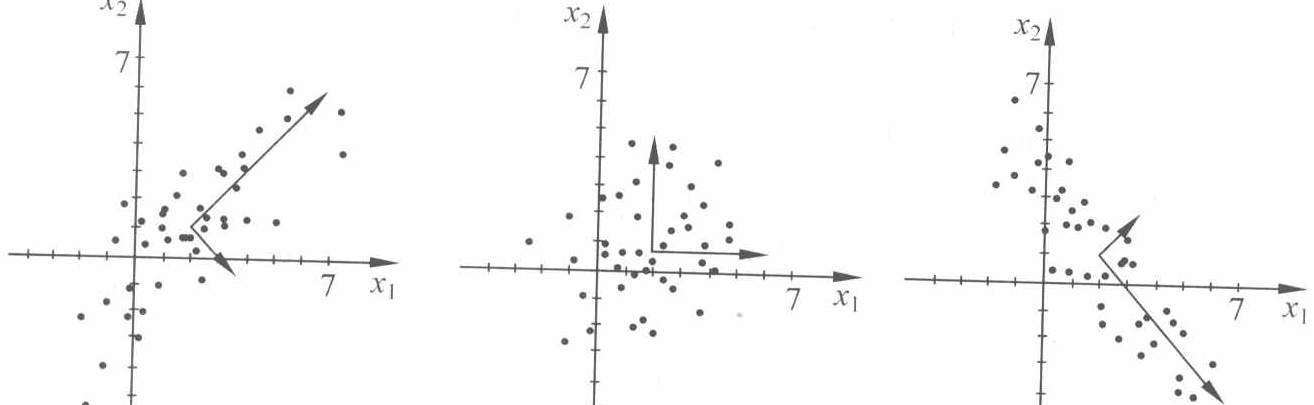
\includegraphics[width=111.3mm]{figs/fig_pg110_1.png}
\phantomsection\label{fig:3.8}\mvcap{图 3.8\quad 图 3.7 中散布图的 $95\%$ 均值中心椭圆的轴}
\end{mvfigure}

接下来, 对于
\[
\mathbf{S}=\begin{bmatrix}3&0\\0&3\end{bmatrix},\ \text{特征值满足}\quad 0=(\lambda-3)^{2}
\]
我们任意地选择特征向量为 $\lambda_{1}=3,\mathbf{e}_{1}'=[1,0]$ 和 $\lambda_{2}=3,\mathbf{e}_{2}'=[0,1]$, 向量 $\sqrt{3}\times\sqrt{5.99}\,\mathbf{e}_{1}$ 和 $\sqrt{3}\times\sqrt{5.99}\,\mathbf{e}_{2}$ 如\hyperref[fig:3.8]{图 3.8}(b) 所示.

最后, 对于
\[
\mathbf{S}=\begin{bmatrix}5&-4\\-4&5\end{bmatrix},\ \text{特征值满足}\quad 0=(\lambda-5)^{2}-(-4)^{2}=(\lambda-9)(\lambda-1)
\]
我们确定特征值-特征向量对 $\lambda_{1}=9,\mathbf{e}_{1}'=[1/\sqrt{2},-1/\sqrt{2}]$ 和 $\lambda_{2}=1,\mathbf{e}_{2}'=[1/\sqrt{2},1/\sqrt{2}]$. 换算特征向量 $3\sqrt{5.99}\,\mathbf{e}_{1}$ 和 $\sqrt{5.99}\,\mathbf{e}_{2}$ 如\hyperref[fig:3.8]{图 3.8}(c) 所示.

在二维中, 经常可以用眼睛看出均值中心椭圆的轴. 然而, 对于不能直观地检验的高维数据特征向量方法也有效.

注意: 这里广义方差 $|\mathbf{S}|$ 对所有三个模型给出同一值 $|\mathbf{S}|=9$. 但广义方差不包含有关图形定向的任何信息. 当进行比较的两个或更多个样本 (模型) 有几乎相同的定向时, 广义方差更容易解释.

注意到我们的三个散布图覆盖了大约相同的区域. 由于所有的 $|\mathbf{S}|=9$, 因此概括变化性的椭圆
\[
(\mathbf{x}-\bar{\mathbf{x}})'\mathbf{S}^{-1}(\mathbf{x}-\bar{\mathbf{x}})\le c^{2}
\]
恰好有相同的区域 [参见\hyperref[eq:3-17]{式(3-17)}].

正如\hyperref[fig:3.8]{图 3.8} 所表明的, 不能由 $|\mathbf{S}|$ 发现不同的相关结构. 对于 $p>2$ 的情况, 甚至可能更加模糊.\hfill$\blacksquare$

%% ===== pg-111 =====

因此, 经常希望不仅仅用单一数 $|\mathbf{S}|$ 作为 $\mathbf{S}$ 的一个概括量. 从练习 2.12 可知, $|\mathbf{S}|$ 可以表示为 $\mathbf{S}$ 的特征值的乘积 $\lambda_{1}\lambda_{2}\cdots\lambda_{p}$. 而且, 基于 $\mathbf{S}^{-1}$ 的均值中心椭球[参见\hyperref[eq:3-16]{式(3-16)}]具有长度与 $\lambda$ 的平方根成比例的轴(参考 2.3 节). 因此, 这些特征值提供了在 $p$ 维空间中表现数据在所有方向上变化性的信息. 所以, 报告它们的个别值与它们的乘积一样是有用的. 以后当我们讨论主成分时, 将连续这个题目.

\mvsub{广义样本方差为零的情况}

在某些情况中, 广义样本方差将是零. 在偏差矩阵
\phantomsection\label{eq:3-18}
\begin{equation}
\begin{aligned}
\begin{bmatrix}\mathbf{x}'_{1}-\bar{\mathbf{x}}'\\[2pt]\mathbf{x}'_{2}-\bar{\mathbf{x}}'\\[2pt]\vdots\\[2pt]\mathbf{x}'_{n}-\bar{\mathbf{x}}'\end{bmatrix}_{(n\times p)}
&=\begin{bmatrix}x_{11}-\bar{x}_{1}&x_{12}-\bar{x}_{2}&\cdots&x_{1p}-\bar{x}_{p}\\[2pt]x_{21}-\bar{x}_{1}&x_{22}-\bar{x}_{2}&\cdots&x_{2p}-\bar{x}_{p}\\[2pt]\vdots&\vdots&&\vdots\\[2pt]x_{n1}-\bar{x}_{1}&x_{n2}-\bar{x}_{2}&\cdots&x_{np}-\bar{x}_{p}\end{bmatrix}\\[6pt]
&=\underset{(n\times p)}{\mathbf{X}-\dfrac{1}{n}\mathbf{1}\bar{\mathbf{x}}'}
\end{aligned}
\tag{3-18}
\end{equation}
至少有一列可表示为其他列的线性组合时, 一个为零的广义方差表示极值退化. 正如我们曾经从几何上说明过的, 这是偏差向量之一——例如 $\mathbf{d}'_{i}=[x_{i1}-\bar{x}_{1},\cdots,x_{ip}-\bar{x}_{p}]$——位于由 $\mathbf{d}_{1},\cdots,\mathbf{d}_{i-1},\mathbf{d}_{i+1},\cdots,\mathbf{d}_{n}$ 生成的(超)平面内.

\mvthm{结论 3.2}{广义方差为零, 当且仅当至少一个偏差向量位于由其他向量的所有线性组合形成的(超)平面内——也就是说, \hyperref[eq:3-18]{式(3-18)} 中的偏差矩阵的列线性相关.}

\noindent\mvbold{证明}\quad 如果偏差矩阵 $(\mathbf{X}-\frac{1}{n}\mathbf{1}\bar{\mathbf{x}}')$ 的列是线性相关的, 存在一个列的线性组合使得
\begin{align*}
0&=a_{1}\cdot\text{列}_{1}(\mathbf{X}-\tfrac{1}{n}\mathbf{1}\bar{\mathbf{x}}')+\cdots+a_{p}\cdot\text{列}_{p}(\mathbf{X}-\tfrac{1}{n}\mathbf{1}\bar{\mathbf{x}}')\\
&=(\mathbf{X}-\tfrac{1}{n}\mathbf{1}\bar{\mathbf{x}}')\mathbf{a}\qquad\text{对某个}\ \mathbf{a}\ne0
\end{align*}
但是, 正如可以证明 $(n-1)\mathbf{S}=(\mathbf{X}-\frac{1}{n}\mathbf{1}\bar{\mathbf{x}}')'(\mathbf{X}-\frac{1}{n}\mathbf{1}\bar{\mathbf{x}}')$ 和 $(n-1)\mathbf{S}\mathbf{a}=(\mathbf{X}-\frac{1}{n}\mathbf{1}\bar{\mathbf{x}}')'(\mathbf{X}-\frac{1}{n}\mathbf{1}\bar{\mathbf{x}}')\mathbf{a}=0$ 一样, 同样的 $\mathbf{a}$, 在 $\mathbf{S}$ 的列中对应于一个线性相关性 $a_{1}\cdot\text{列}_{1}(\mathbf{S})+\cdots+a_{p}\cdot\text{列}_{p}(\mathbf{S})=\mathbf{S}\mathbf{a}=0$. 因此, 由结论 2A.9, $|\mathbf{S}|=0$.

另一方面, 如果 $|\mathbf{S}|=0$, 则存在 $\mathbf{S}$ 的列的某个线性组合 $\mathbf{S}\mathbf{a}$, 使得 $\mathbf{S}\mathbf{a}=0$, 即 $0=(n-1)\mathbf{S}\mathbf{a}=(\mathbf{X}-\frac{1}{n}\mathbf{1}\bar{\mathbf{x}}')'(\mathbf{X}-\frac{1}{n}\mathbf{1}\bar{\mathbf{x}}')\mathbf{a}$. 用 $\mathbf{a}'$ 左乘得
\[
0=\mathbf{a}'(\mathbf{X}-\tfrac{1}{n}\mathbf{1}\bar{\mathbf{x}}')'(\mathbf{X}-\tfrac{1}{n}\mathbf{1}\bar{\mathbf{x}}')\mathbf{a}=L^{2}_{1\times1}
\]
且因为长度等于零, 必须有 $(\mathbf{X}-\frac{1}{n}\mathbf{1}\bar{\mathbf{x}}')\mathbf{a}=0$. 因此, $(\mathbf{X}-\frac{1}{n}\mathbf{1}\bar{\mathbf{x}}')$ 的列是线性相关的.\hfill$\blacksquare$

\noindent\textbf{例 3.9}\quad (广义方差为零的一个实例)

对
\[
\underset{(3\times3)}{\mathbf{X}}=\begin{bmatrix}1&2&5\\4&1&6\\4&0&4\end{bmatrix}
\]
证明 $|\mathbf{S}|=0$ 且确定退化.

这里 $\bar{\mathbf{x}}'=[3,1,5]$, 因此
\[
\mathbf{X}-\mathbf{1}\bar{\mathbf{x}}'=\begin{bmatrix}1-3&2-1&5-5\\4-3&1-1&6-5\\4-3&0-1&4-5\end{bmatrix}=\begin{bmatrix}-2&1&0\\1&0&1\\1&-1&-1\end{bmatrix}
\]

%% ===== pg-112 =====

% ---- pg-112 （书页 100） ----

偏差(列)向量为 $\mathbf{d}'_{1}=[-2,1,1], \mathbf{d}'_{2}=[1,0,-1]$ 和 $\mathbf{d}'_{3}=[0,1,-1]$. 由于 $\mathbf{d}_{3}=\mathbf{d}_{1}+2\mathbf{d}_{2}$, 有列退化(注意也有行退化). 这意味着偏差向量之一, 例如 $\mathbf{d}_{3}$, 位于其他两个剩余向量生成的平面内. 因此, 三维体积是零. 这情况如\hyperref[fig:3.9]{图 3.9} 所示, 并可以通过证明 $|\mathbf{S}|=0$ 作代数检验. 我们有

\begin{mvfigure}
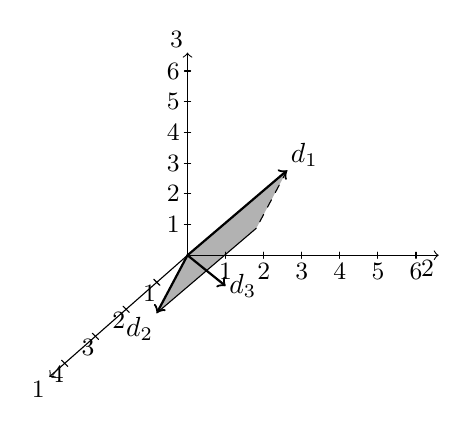
\begin{tikzpicture}[scale=0.78,line join=round,line cap=round]
% 坐标基: 轴1 单位向量 (-0.50,-0.44), 轴2 单位向量 (0.62,0), 轴3 单位向量 (0,0.50)
% 向量: d1=(-2,1,1) d2=(1,0,-1) d3=(0,1,-1)
% 阴影: 由 d1 与 d2 张成的平行四边形
\fill[black!30] (0,0) -- (1.62,1.38) -- (1.12,0.44) -- (-0.50,-0.94) -- cycle;
\draw[dashed] (1.62,1.38) -- (1.12,0.44);
\draw (1.12,0.44) -- (-0.50,-0.94);
% 轴2
\draw[->] (0,0) -- (4.09,0);
\foreach \k in {1,...,6} {
  \draw (0.62*\k,-0.05) -- (0.62*\k,0.05);
  \node[below,inner sep=1.5pt,font=\small] at (0.62*\k,-0.05) {\k};
}
\node[below left,inner sep=1.5pt,font=\small] at (4.09,0) {2};
% 轴3
\draw[->] (0,0) -- (0,3.30);
\foreach \k in {1,...,6} {
  \draw (-0.05,0.5*\k) -- (0.05,0.5*\k);
  \node[left,inner sep=1.5pt,font=\small] at (-0.05,0.5*\k) {\k};
}
\node[above left,inner sep=1.5pt,font=\small] at (0,3.30) {3};
% 轴1
\draw[->] (0,0) -- (-2.25,-1.98);
\foreach \k in {1,...,4} {
  \draw (-0.50*\k+0.05,-0.44*\k-0.05) -- (-0.50*\k-0.05,-0.44*\k+0.05);
}
\node[font=\small] at (-0.62,-0.62) {1};
\node[font=\small] at (-1.12,-1.06) {2};
\node[font=\small] at (-1.62,-1.50) {3};
\node[font=\small] at (-2.12,-1.94) {4};
\node[below left,inner sep=1.5pt,font=\small] at (-2.25,-1.98) {1};
% 向量
\draw[->,thick] (0,0) -- (1.62,1.38) node[above right,inner sep=1pt] {$d_{1}$};
\draw[->,thick] (0,0) -- (-0.50,-0.94) node[below left,inner sep=1pt] {$d_{2}$};
\draw[->,thick] (0,0) -- (0.62,-0.50) node[right,inner sep=1pt] {$d_{3}$};
\end{tikzpicture}
\phantomsection\label{fig:3.9}\mvcap{图 3.9\quad 三维体积为零的一个实例($|\mathbf{S}|=0$)}
\end{mvfigure}

\[
\underset{(3\times3)}{\mathbf{S}}=\begin{bmatrix}3&-\dfrac{3}{2}&0\\[3pt]-\dfrac{3}{2}&1&\dfrac{1}{2}\\[3pt]0&\dfrac{1}{2}&1\end{bmatrix}
\]

并从定义 2A.24,
\begin{align*}
|\mathbf{S}|&=3\begin{vmatrix}1&\frac{1}{2}\\\frac{1}{2}&1\end{vmatrix}(-1)^{2}+\left(-\frac{3}{2}\right)\begin{vmatrix}-\frac{3}{2}&\frac{1}{2}\\0&1\end{vmatrix}(-1)^{3}+0\begin{vmatrix}-\frac{3}{2}&1\\0&\frac{1}{2}\end{vmatrix}(-1)^{4}\\
&=3\times\left(1-\frac{1}{4}\right)+\frac{3}{2}\times\left(-\frac{3}{2}-0\right)+0=\frac{9}{4}-\frac{9}{4}=0\qquad\blacksquare
\end{align*}

当用电子化方式传送和接收大的数据集时, 研究者有时会意外发现零广义方差的情况, 使得 $\mathbf{S}$ 没有逆. 我们曾遇到这样的情况, 而且在未弄明情况以前会带来困难. 例如, 当数据是许多测验分数并且研究者已经把是其他变量之和的变量也包含进来时, 一个奇异的协方差矩阵就出现了. 比如说, 代数分数与几何分数可以合起来给出一个总的数学分数, 或随堂期中测验和期末考试分数加起来得到总成绩. 再如, 许多化学制品的总重量已包括了每个分量的重量.

由诸原始变量之和产生新变量, 并把它们都包含在数据集中, 这种常见做法会使我们失去了大量时间, 因而必须强调这种后果.

\noindent\textbf{例 3.10}\quad (产生的新变量会导致零广义方差)

考虑数据矩阵
\[
\mathbf{X}=\begin{bmatrix}1&9&10\\4&12&16\\2&10&12\\5&8&13\\3&11&14\end{bmatrix}
\]
其中第三列是第一、二列之和. 这些数据分别是钟点雇工和全时雇工每天成功的电话求职个数. 这样, 第三列是每天成功求职的总数.

证明广义方差 $|\mathbf{S}|=0$, 并确定数据的自然相关性.

我们求得每一项为 $x_{ik}-\bar{x}_{k}$ 的被均值修正的数据矩阵, 是
\[
\mathbf{X}-\mathbf{1}\bar{\mathbf{x}}'=\begin{bmatrix}-2&-1&-3\\1&2&3\\-1&0&-1\\2&-2&0\\0&1&1\end{bmatrix}
\]

%% ===== pg-113 =====

% ---- pg-113 （书页 101） ----

所得到的协方差矩阵是
\[
\mathbf{S}=\begin{bmatrix}2.5&0&2.5\\0&2.5&2.5\\2.5&2.5&5.0\end{bmatrix}
\]

此时, 我们证明广义方差为零即
\[
|\mathbf{S}|=2.5^{2}\times5+0+0-2.5^{3}-2.5^{3}-0=0
\]

一般的, 如果数据矩阵 $\mathbf{X}$ 的三列满足线性约束 $a_{1}x_{j1}+a_{2}x_{j2}+a_{3}x_{j3}=c$ 对所有 $j$ 为常数, 则 $a_{1}\bar{x}_{1}+a_{2}\bar{x}_{2}+a_{3}\bar{x}_{3}=c$, 因此, 对所有 $j$, 有
\[
a_{1}(x_{j1}-\bar{x}_{1})+a_{2}(x_{j2}-\bar{x}_{2})+a_{3}(x_{j3}-\bar{x}_{3})=0
\]
即
\[
(\mathbf{X}-\mathbf{1}\bar{\mathbf{x}}')\mathbf{a}=\mathbf{0}
\]
且被均值修正的数据矩阵的列是线性相关的. 于是, 把与第一、二个有线性关系的第三个变量包括进来, 导致广义方差为零. 只要当被均值修正的数据矩阵的列线性相关,
\[
(n-1)\mathbf{S}\mathbf{a}=(\mathbf{X}-\mathbf{1}\bar{\mathbf{x}}')'(\mathbf{X}-\mathbf{1}\bar{\mathbf{x}}')\mathbf{a}=(\mathbf{X}-\mathbf{1}\bar{\mathbf{x}}')\mathbf{0}=\mathbf{0}
\]
且 $\mathbf{S}\mathbf{a}=\mathbf{0}$ 确定了 $\mathbf{S}$ 的列的线性相关性. 因此 $|\mathbf{S}|=0$.

因为 $\mathbf{S}\mathbf{a}=\mathbf{0}=0\mathbf{a}$, 可见, $\mathbf{a}$ 是 $\mathbf{S}$ 的一个与特征值零相对应的换算过的特征向量. 这导致一个重要的诊断方法: 如果我们没意识到任一多余变量是其余变量的线性组合, 我们可以通过计算 $\mathbf{S}$ 的特征向量并辨别出与零特征值相对应的那一个, 找到它们. 即如果我们没意识到此例中的相关性, 由于
\[
\mathbf{S}\mathbf{a}=\begin{bmatrix}2.5&0&2.5\\0&2.5&2.5\\2.5&2.5&5.0\end{bmatrix}\begin{bmatrix}1\\1\\-1\end{bmatrix}=\begin{bmatrix}0\\0\\0\end{bmatrix}=0\begin{bmatrix}1\\1\\-1\end{bmatrix}
\]
计算机计算会找到一个与特征向量 $\mathbf{a}'=[1,1,-1]$ 相应的特征值.

系数揭示了对所有 $j$ 有
\[
1(x_{j1}-\bar{x}_{1})+1(x_{j2}-\bar{x}_{2})+(-1)(x_{j3}-\bar{x}_{3})=0
\]
而且, 对所有 $n$ 个单位元前两个变量的和减第三个变量后是一常数 $c$. 这里第三个变量实际上是前两个变量之和, 所以原始数据矩阵的列满足 $c=0$ 时的一个线性约束. 因为 $c=0$ 这一特殊情况, 该约束确定了数据矩阵的列是线性相关这一事实.

我们对上述例子中讨论的广义方差为零的情况, 可以总结出重要的等价条件. 无论何时, 只要非零向量 $\mathbf{a}$ 满足下列三个条件之一, 它就满足所有三个条件:

\begin{mvtable}
\begin{tabular}{@{}p{0.30\linewidth}@{}p{0.33\linewidth}@{}p{0.35\linewidth}@{}}
$\underbrace{(1)\ \mathbf{S}\mathbf{a}=\mathbf{0}}_{\substack{\text{\footnotesize $a$ 是与特征值零}\\\text{\footnotesize 对应的 $\mathbf{S}$ 的一个换}\\\text{\footnotesize 算过的特征向量.}}}$
&
$\underbrace{(2)\ \mathbf{a}'(\mathbf{x}_{j}-\bar{\mathbf{x}})=\mathbf{0},\ \text{对所有 } j}_{\substack{\text{\footnotesize 利用 $a$, 被均值修正的数据}\\\text{\footnotesize 的线性组合为零.}}}$
&
$\underbrace{(3)\ \mathbf{a}'\mathbf{x}_{j}=c,\ \text{对所有 } j\quad(c=\mathbf{a}'\bar{\mathbf{x}})}_{\substack{\text{\footnotesize 利用 $a$, 原始数据的}\\\text{\footnotesize 线性组合是常数.}}}$
\end{tabular}
\end{mvtable}

我们已证明, 若满足条件(3)——即若一个变量的值可以用其余变量来表示——则由于 $\mathbf{S}$ 有一个零特征值, 所以广义方差为零. 另一方面, 若条件(1)成立, 则特征向量 $\mathbf{a}$ 对被均值修正的数据的线性相关性给出了系数.

在任何统计分析中, $|\mathbf{S}|=0$ 就数学计算而论, 意味着某些变量的测量结果应从研究中除去. 所得的对应数据矩阵将化为一个满秩的协方差矩阵, 广义方差不为零. 在退化的情况下哪

%% ===== pg-114 =====

% ---- pg-114 （书页 102） ----

些测量结果应除去, 这一问题并不容易回答. 在有选择时, 我们应保留表示原因的(假定)变量, 而不是那些次要特征变量的测量结果. 在主成分的讨论中, 将再次讲到这个问题.

此刻, 我们暂时只描述 $\mathbf{S}$ 为满秩或降秩的一些简单条件.

\mvthm{结论 3.3}{如果 $n\le p$, 即(样本大小)$\le$(变量的个数), 则对所有样本有 $|\mathbf{S}|=0$.}

\noindent\textbf{证明}\quad 我们必须证明 $\mathbf{S}$ 的秩小于或等于 $p$, 然后应用结论 2A.9.

对任何固定样本, \hyperref[eq:3-18]{式(3-18)}的 $n$ 个行向量加起来是零向量. 这个线性组合的存在, 意味着 $\mathbf{X}-\mathbf{1}\bar{\mathbf{x}}'$ 的秩小于或等于 $n-1$, 又因为 $n\le p$, 所以秩小于或等于 $p-1$. 由于
\[
(n-1)\underset{(p\times p)}{\mathbf{S}}=\underset{(p\times n)}{(\mathbf{X}-\mathbf{1}\bar{\mathbf{x}}')'}\underset{(n\times p)}{(\mathbf{X}-\mathbf{1}\bar{\mathbf{x}}')}
\]
$\mathbf{S}$ 的第 $k$ 列, 列$_{k}(\mathbf{S})$, 可写成 $(\mathbf{X}-\mathbf{1}\bar{\mathbf{x}}')'$ 的行的一个线性组合, 具体的,
\begin{align*}
(n-1)\cdot\text{列}_{k}(\mathbf{S})&=(\mathbf{X}-\mathbf{1}\bar{\mathbf{x}}')'\cdot\text{列}_{k}(\mathbf{X}-\mathbf{1}\bar{\mathbf{x}}')\\
&=(x_{1k}-\bar{x}_{k})\cdot\text{行}_{1}(\mathbf{X}-\mathbf{1}\bar{\mathbf{x}}')'+\cdots+(x_{nk}-\bar{x}_{k})\cdot\text{行}_{n}(\mathbf{X}-\mathbf{1}\bar{\mathbf{x}}')'
\end{align*}
由于 $(\mathbf{X}-\mathbf{1}\bar{\mathbf{x}}')'$ 的行向量加起来是零向量, 我们可以把行$_{1}(\mathbf{X}-\mathbf{1}\bar{\mathbf{x}}')'$写为剩余行向量之和的负值. 将它代入上述方程式的行$_{1}(\mathbf{X}-\mathbf{1}\bar{\mathbf{x}}')'$中, 列$_{k}(\mathbf{S})$可表示为至多 $n-1$ 个线性独立的行向量行$_{2}(\mathbf{X}-\mathbf{1}\bar{\mathbf{x}}')',\cdots$, 行$_{n}(\mathbf{X}-\mathbf{1}\bar{\mathbf{x}}')'$ 的一个线性组合. 因此, $\mathbf{S}$ 的秩小于或等于 $n-1$——如同在证明开始时所指明的——小于或等于 $p-1$, 且 $\mathbf{S}$ 是奇异的. 这就意味着, 由结论 2A.9, $|\mathbf{S}|=0$.\hfill$\blacksquare$

\mvthm{结论 3.4}{设行向量 $\mathbf{x}_{1},\mathbf{x}_{2},\cdots,\mathbf{x}_{n}$ 是独立的随机向量 $\mathbf{X}_{1},\mathbf{X}_{2},\cdots,\mathbf{X}_{n}$ 的实现, 其中 $\mathbf{x}'_{j}$ 是数据矩阵 $\mathbf{X}$ 的第 $j$ 行. 则}

1.\quad 若对于每个常数向量 $\mathbf{a}\ne\mathbf{0}$, 线性组合 $\mathbf{a}'\mathbf{X}_{j}$ 有正方差, 则在 $p<n$ 时, $\mathbf{S}$ 以概率 1 满秩且 $|\mathbf{S}|>0$.

2.\quad 若对所有 $j$, $\mathbf{a}'\mathbf{X}_{j}$ 以概率 1 为常数(例如, $c$), 则 $|\mathbf{S}|=0$.

\noindent\textbf{证明}\quad (2) 若以概率 1 有 $\mathbf{a}'\mathbf{X}_{j}=a_{1}X_{j1}+a_{2}X_{j2}+\cdots+a_{p}X_{jp}=c$, 则对所有 $j$, $\mathbf{a}'\mathbf{x}_{j}=c$, 且该线性组合的样本均值是 $\bar{c}=\sum_{j=1}^{n}(a_{1}x_{j1}+a_{2}x_{j2}+\cdots+a_{p}x_{jp})/n=a_{1}\bar{x}_{1}+a_{2}\bar{x}_{2}+\cdots+a_{p}\bar{x}_{p}=\mathbf{a}'\bar{\mathbf{x}}$. 那么,
\begin{align*}
(\mathbf{X}-\mathbf{1}\bar{\mathbf{x}}')\mathbf{a}&=a_{1}\begin{bmatrix}x_{11}-\bar{x}_{1}\\\vdots\\x_{n1}-\bar{x}_{1}\end{bmatrix}+\cdots+a_{p}\begin{bmatrix}x_{1p}-\bar{x}_{p}\\\vdots\\x_{np}-\bar{x}_{p}\end{bmatrix}\\
&=\begin{bmatrix}\mathbf{a}'\mathbf{x}_{1}-\mathbf{a}'\bar{\mathbf{x}}\\\vdots\\\mathbf{a}'\mathbf{x}_{n}-\mathbf{a}'\bar{\mathbf{x}}\end{bmatrix}=\begin{bmatrix}c-c\\\vdots\\c-c\end{bmatrix}=\mathbf{0}
\end{align*}
表明线性相关; 由结论 3.2 得出结论成立.

(1) 的证明很困难, 可以在文献[2]中找到.\hfill$\blacksquare$

\mvsub{由 $|\mathbf{R}|$ 确定广义方差及其几何解释}

广义样本方差受到单个变量观测结果的变化性的过度影响. 例如, 假定某个 $s_{ii}$ 或者大或者很小. 从几何上看, 对应的偏差向量 $\mathbf{d}_{i}=(\mathbf{y}_{i}-\bar{x}_{i}\mathbf{1})$ 会很长或很短, 因而在确定体积时很明显地是一个重要因素. 因此, 有时改变所有偏差向量的比例, 使它们有相同的长度, 是有用的.

%% ===== pg-115 =====

% ---- pg-115 （书页 103） ----

改变剩余向量的比例, 相当于对每一个原始的观测值 $x_{ik}$ 用它的标准化值 $(x_{ik}-\bar{x}_{k})/\sqrt{s_{kk}}$ 替换. 标准化变量的样本协方差矩阵就是 $\mathbf{R}$, 即原始变量的样本相关阵(参考练习 3.13). 我们定义
\begin{mvbox}
\phantomsection\label{eq:3-19}
\begin{equation}
(\text{标准化变量的广义样本方差})=|\mathbf{R}| \tag{3-19}
\end{equation}
\end{mvbox}
由于所得到的向量
\[
[(x_{1k}-\bar{x}_{k})/\sqrt{s_{kk}},(x_{2k}-\bar{x}_{k})/\sqrt{s_{kk}},\cdots,(x_{nk}-\bar{x}_{k})/\sqrt{s_{kk}}]=(\mathbf{y}_{k}-\bar{x}_{k}\mathbf{1})'/\sqrt{s_{kk}}
\]
的长度都为 $\sqrt{n-1}$, 当这些向量几乎正交时, 标准化变量的广义样本方差较大, 而当这些向量的两个或更多个几乎是同一方向时, 广义样本方差较小. 利用推导出\hyperref[eq:3-7]{式(3-7)}的方法, 容易求出 $(\mathbf{y}_{i}-\bar{x}_{i}\mathbf{1})/\sqrt{s_{ii}}$ 和 $(\mathbf{y}_{k}-\bar{x}_{k}\mathbf{1})/\sqrt{s_{kk}}$ 之间夹角 $\theta_{ik}$ 的余弦是样本相关系数 $r_{ik}$. 因此, 我们可以作出结论: 当所有 $r_{ik}$ 接近零时, $|\mathbf{R}|$ 较大, 而当 $r_{ik}$ 中一个或多个是接近 1 或 $-1$ 时, $|\mathbf{R}|$ 较小.

总而言之, 有如下结论: 设
\[
\frac{(\mathbf{y}_{i}-\bar{x}_{i}\mathbf{1})}{\sqrt{s_{ii}}}=\begin{bmatrix}\dfrac{x_{1i}-\bar{x}_{i}}{\sqrt{s_{ii}}}\\\dfrac{x_{2i}-\bar{x}_{i}}{\sqrt{s_{ii}}}\\\vdots\\\dfrac{x_{ni}-\bar{x}_{i}}{\sqrt{s_{ii}}}\end{bmatrix},\quad i=1,2,\cdots,p
\]
是标准化变量的偏差向量. 这些偏差向量在 $\mathbf{d}_{i}$ 的方向上, 而长度平方为 $n-1$. 在 $p$ 维空间中由偏差向量生成的体积, 与广义样本方差有关. 采用与推导\hyperref[eq:3-15]{式(3-15)}同样的步骤, 有:
\phantomsection\label{eq:3-20}
\begin{equation}
\left(\begin{matrix}\text{标准化变量的}\\\text{广义样本方差}\end{matrix}\right)=|\mathbf{R}|=(n-1)^{-p}(\text{体积})^{2} \tag{3-20}
\end{equation}

对于\hyperref[fig:3.6]{图 3.6} 中的偏差向量, 标准化变量的偏差向量所形成的体积, 如\hyperref[fig:3.10]{图 3.10} 所示. 比较\hyperref[fig:3.10]{图 3.10} 与\hyperref[fig:3.6]{图 3.6}, 显示出 $\mathbf{d}_{2}$ 向量(在 $x_{2}$ 上较大的变化性)对体积平方 $|\mathbf{S}|$ 的影响比它对体积平方 $|\mathbf{R}|$ 的影响大得多.

\begin{mvfigure}
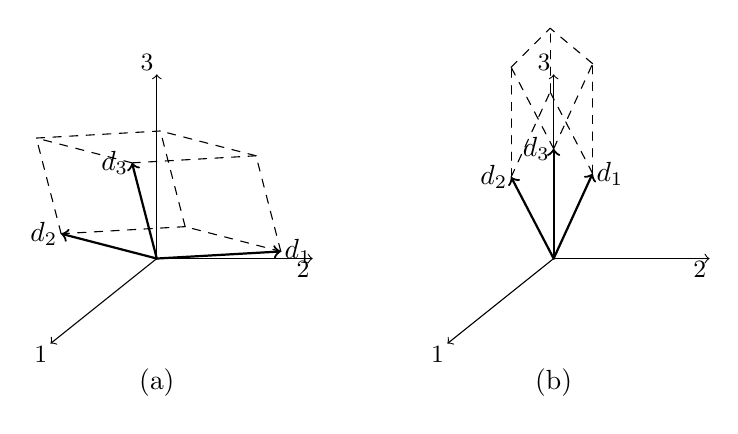
\begin{tikzpicture}[scale=0.9,line join=round,line cap=round]
% ---------- (a) 原偏差向量 ----------
\begin{scope}
\draw[->] (0,0) -- (2.20,0) node[below left,inner sep=1pt,font=\small] {2};
\draw[->] (0,0) -- (0,2.60) node[above left,inner sep=1pt,font=\small] {3};
\draw[->] (0,0) -- (-1.50,-1.20) node[below left,inner sep=1pt,font=\small] {1};
\draw[->,thick] (0,0) -- (1.75,0.10) node[right,inner sep=1pt] {$d_{1}$};
\draw[->,thick] (0,0) -- (-1.35,0.35) node[left,inner sep=1pt] {$d_{2}$};
\draw[->,thick] (0,0) -- (-0.35,1.35) node[left,inner sep=1pt] {$d_{3}$};
% 平行六面体（虚线）
\draw[dashed] (1.75,0.10) -- (0.40,0.45);
\draw[dashed] (-1.35,0.35) -- (0.40,0.45);
\draw[dashed] (1.75,0.10) -- (1.40,1.45);
\draw[dashed] (-0.35,1.35) -- (1.40,1.45);
\draw[dashed] (-1.35,0.35) -- (-1.70,1.70);
\draw[dashed] (-0.35,1.35) -- (-1.70,1.70);
\draw[dashed] (0.40,0.45) -- (0.05,1.80);
\draw[dashed] (1.40,1.45) -- (0.05,1.80);
\draw[dashed] (-1.70,1.70) -- (0.05,1.80);
\node at (0,-1.75) {(a)};
\end{scope}
% ---------- (b) 标准化偏差向量 ----------
\begin{scope}[xshift=5.6cm]
\draw[->] (0,0) -- (2.20,0) node[below left,inner sep=1pt,font=\small] {2};
\draw[->] (0,0) -- (0,2.60) node[above left,inner sep=1pt,font=\small] {3};
\draw[->] (0,0) -- (-1.50,-1.20) node[below left,inner sep=1pt,font=\small] {1};
\draw[->,thick] (0,0) -- (0.55,1.20) node[right,inner sep=1pt] {$d_{1}$};
\draw[->,thick] (0,0) -- (-0.60,1.15) node[left,inner sep=1pt] {$d_{2}$};
\draw[->,thick] (0,0) -- (0.00,1.55) node[left,inner sep=1pt] {$d_{3}$};
% 平行六面体（虚线）
\draw[dashed] (0.55,1.20) -- (-0.05,2.35);
\draw[dashed] (-0.60,1.15) -- (-0.05,2.35);
\draw[dashed] (0.55,1.20) -- (0.55,2.75);
\draw[dashed] (0.00,1.55) -- (0.55,2.75);
\draw[dashed] (-0.60,1.15) -- (-0.60,2.70);
\draw[dashed] (0.00,1.55) -- (-0.60,2.70);
\draw[dashed] (-0.05,2.35) -- (-0.05,3.25);
\draw[dashed] (0.55,2.75) -- (-0.05,3.25);
\draw[dashed] (-0.60,2.70) -- (-0.05,3.25);
\node at (0,-1.75) {(b)};
\end{scope}
\end{tikzpicture}
\phantomsection\label{fig:3.10}\mvcap{图 3.10\quad 由标准化变量的等长度偏差向量生成的体积}
\end{mvfigure}

%% ===== pg-116 =====

% ---- pg-116 （书页 104） ----

量 $|\mathbf{S}|$ 和 $|\mathbf{R}|$ 通过关系
\phantomsection\label{eq:3-21}
\begin{equation}
|\mathbf{S}|=(s_{11}s_{22}\cdots s_{pp})|\mathbf{R}| \tag{3-21}
\end{equation}
相联系, 因此
\phantomsection\label{eq:3-22}
\begin{equation}
(n-1)^{p}|\mathbf{S}|=(n-1)^{p}(s_{11}s_{22}\cdots s_{pp})|\mathbf{R}| \tag{3-22}
\end{equation}
[\hyperref[eq:3-21]{式(3-21)}的证明作为练习 3.12, 留给读者.]

用体积解释\hyperref[eq:3-22]{式(3-22)}, 从\hyperref[eq:3-15]{式(3-15)}和\hyperref[eq:3-20]{式(3-20)}可见, 体积平方 $(n-1)^{-p}|\mathbf{S}|$ 与体积平方 $(n-1)^{-p}|\mathbf{R}|$ 成比例. 比例常数是方差的乘积, 而它同样也正比于 $\mathbf{d}_{i}$ 的长度 $(n-1)s_{ii}$ 的平方之积. \hyperref[eq:3-21]{式(3-21)}从代数上说明了对 $x_{1}$ 等量的标度的变化如何改变广义方差之间的关系. 因为 $|\mathbf{R}|$ 是基于标准化测量值, 它不会受到标度变化的影响. 然而, 每当乘积因子 $s_{ii}$ 变化时, $|\mathbf{S}|$ 的相对值将随之改变.

\noindent\textbf{例 3.11}\quad (说明 $|\mathbf{S}|$ 与 $|\mathbf{R}|$ 之间的关系)

让我们来说明当 $p=3$ 时, 广义方差 $|\mathbf{S}|$ 与 $|\mathbf{R}|$ 在\hyperref[eq:3-21]{式(3-21)}中的关系. 设
\[
\underset{(3\times3)}{\mathbf{S}}=\begin{bmatrix}4&3&1\\3&9&2\\1&2&1\end{bmatrix}
\]
则 $s_{11}=4$, $s_{22}=9$ 和 $s_{33}=1$. 而且,
\[
\mathbf{R}=\begin{bmatrix}1&\dfrac{1}{2}&\dfrac{1}{2}\\[4pt]\dfrac{1}{2}&1&\dfrac{2}{3}\\[4pt]\dfrac{1}{2}&\dfrac{2}{3}&1\end{bmatrix}
\]
利用定义 2A.24, 我们得到
\begin{align*}
|\mathbf{S}|&=4\begin{vmatrix}9&2\\2&1\end{vmatrix}(-1)^{2}+3\begin{vmatrix}3&2\\1&1\end{vmatrix}(-1)^{3}+1\begin{vmatrix}3&9\\1&2\end{vmatrix}(-1)^{4}\\
&=4\times(9-4)-3\times(3-2)+1\times(6-9)=14
\end{align*}
\begin{align*}
|\mathbf{R}|&=1\begin{vmatrix}1&\frac{2}{3}\\\frac{2}{3}&1\end{vmatrix}(-1)^{2}+\frac{1}{2}\begin{vmatrix}\frac{1}{2}&\frac{2}{3}\\\frac{1}{2}&1\end{vmatrix}(-1)^{3}+\frac{1}{2}\begin{vmatrix}\frac{1}{2}&1\\\frac{1}{2}&\frac{2}{3}\end{vmatrix}(-1)^{4}\\
&=\left(1-\frac{4}{9}\right)-\frac{1}{2}\times\left(\frac{1}{2}-\frac{1}{3}\right)+\frac{1}{2}\times\left(\frac{1}{3}-\frac{1}{2}\right)=\frac{7}{18}
\end{align*}
因此有
\[
14=|\mathbf{S}|=s_{11}s_{22}s_{33}|\mathbf{R}|=4\times9\times1\times\frac{7}{18}=14\qquad\text{(检验)}\quad\blacksquare
\]

\mvsub{方差的其他推广}

我们来叙述方差的另一推广形式来结束这一讨论. 具体的, 我们定义总样本方差作为样本方差-协方差矩阵 $\mathbf{S}$ 的对角线元素之和. 这样

\begin{mvbox}
\phantomsection\label{eq:3-23}
\begin{equation}
\text{总样本方差}=s_{11}+s_{22}+\cdots+s_{pp} \tag{3-23}
\end{equation}
\end{mvbox}

\noindent\textbf{例 3.12}\quad (计算总样本方差)

对于例 3.7 和例 3.9 中的方差-协方差矩阵 $\mathbf{S}$ 计算总样本方差.

%% ===== pg-117 =====

% ---- pg-117 （书页 105） ----

从例 3.7,
\[
\mathbf{S}=\begin{bmatrix}252.04&-68.43\\-68.43&123.67\end{bmatrix}
\]
且

总样本方差 $=s_{11}+s_{22}=252.04+123.67=375.71$

从例 3.9,
\[
\mathbf{S}=\begin{bmatrix}3&-\dfrac{3}{2}&0\\[3pt]-\dfrac{3}{2}&1&\dfrac{1}{2}\\[3pt]0&\dfrac{1}{2}&1\end{bmatrix}
\]
且

总样本方差 $=s_{11}+s_{22}+s_{33}=3+1+1=5$\hfill$\blacksquare$

从几何上看, 总样本方差是 $p$ 个偏差向量 $\mathbf{d}_{1}=(\mathbf{y}_{1}-\bar{x}_{1}\mathbf{1}),\cdots,\mathbf{d}_{p}=(\mathbf{y}_{p}-\bar{x}_{p}\mathbf{1})$ 的长度平方之和除以 $n-1$. 总样本方差准则不涉及剩余向量的方向性(相关关系结构). 例如, 它对\hyperref[fig:3.6]{图 3.6}(a)和(b)中剩余向量的两个集合都给定相同的值.

\section{作为矩阵运算的样本均值、协方差与相关系数}  % 原书 3.5
\phantomsection\label{sec:3.5}

我们已提出了数据矩阵 $\mathbf{X}$ 的几何解释, 并导出了描述性统计量 $\bar{\mathbf{x}}$ 和 $\mathbf{S}$. 而且利用矩阵运算, 把对 $\bar{\mathbf{x}}$ 和 $\mathbf{S}$ 的计算从代数上与 $\mathbf{X}$ 直接联系起来是可能的. 简明地描述 $\bar{\mathbf{x}}$, $\mathbf{S}$ 以及整个数据 $\mathbf{X}$ 之间关系的表达式, 很容易在电子计算机上编程. 我们有 $\bar{x}_{i}=(x_{1i}\cdot1+x_{2i}\cdot1+\cdots+x_{ni}\cdot1)/n=\mathbf{y}'_{i}\mathbf{1}/n$. 因此
\[
\bar{\mathbf{x}}=\begin{bmatrix}\bar{x}_{1}\\\bar{x}_{2}\\\vdots\\\bar{x}_{p}\end{bmatrix}=\begin{bmatrix}\dfrac{\mathbf{y}'_{1}\mathbf{1}}{n}\\\dfrac{\mathbf{y}'_{2}\mathbf{1}}{n}\\\vdots\\\dfrac{\mathbf{y}'_{p}\mathbf{1}}{n}\end{bmatrix}=\frac{1}{n}\begin{bmatrix}x_{11}&x_{12}&\cdots&x_{1n}\\x_{21}&x_{22}&\cdots&x_{2n}\\\vdots&\vdots&\ddots&\vdots\\x_{p1}&x_{p2}&\cdots&x_{pn}\end{bmatrix}\begin{bmatrix}1\\1\\\vdots\\1\end{bmatrix}
\]
或
\phantomsection\label{eq:3-24}
\begin{equation}
\bar{\mathbf{x}}=\frac{1}{n}\mathbf{X}'\mathbf{1} \tag{3-24}
\end{equation}
即 $\bar{\mathbf{x}}$ 是由转置数据矩阵右乘向量 $\mathbf{1}$ 后, 再乘常数 $1/n$ 而得到的.

接下来, 我们通过转置\hyperref[eq:3-24]{式(3-24)}的两侧并用 $\mathbf{1}$ 左乘, 建立一个 $n\times p$ 均值矩阵, 即
\phantomsection\label{eq:3-25}
\begin{equation}
\mathbf{1}\bar{\mathbf{x}}'=\frac{1}{n}\mathbf{1}\mathbf{1}'\mathbf{X}=\begin{bmatrix}\bar{x}_{1}&\bar{x}_{2}&\cdots&\bar{x}_{p}\\\bar{x}_{1}&\bar{x}_{2}&\cdots&\bar{x}_{p}\\\vdots&\vdots&\ddots&\vdots\\\bar{x}_{1}&\bar{x}_{2}&\cdots&\bar{x}_{p}\end{bmatrix} \tag{3-25}
\end{equation}
从 $\mathbf{X}$ 减去这一结果, 产生 $n\times p$ 偏差(剩余)矩阵

%% ===== pg-118 =====

% ---- pg-118 （书页 106） ----

\phantomsection\label{eq:3-26}
\begin{equation}
\mathbf{X}-\frac{1}{n}\mathbf{1}\mathbf{1}'\mathbf{X}=\begin{bmatrix}x_{11}-\bar{x}_{1}&x_{12}-\bar{x}_{2}&\cdots&x_{1p}-\bar{x}_{p}\\x_{21}-\bar{x}_{1}&x_{22}-\bar{x}_{2}&\cdots&x_{2p}-\bar{x}_{p}\\\vdots&\vdots&&\vdots\\x_{n1}-\bar{x}_{1}&x_{n2}-\bar{x}_{2}&\cdots&x_{np}-\bar{x}_{p}\end{bmatrix} \tag{3-26}
\end{equation}
现在, 代表平方和与交叉乘积之和的矩阵 $(n-1)\mathbf{S}$, 恰好是\hyperref[eq:3-26]{式(3-26)}矩阵的转置乘以它本身, 或
\begin{align*}
(n-1)\mathbf{S}&=\begin{bmatrix}x_{11}-\bar{x}_{1}&x_{21}-\bar{x}_{1}&\cdots&x_{n1}-\bar{x}_{1}\\x_{12}-\bar{x}_{2}&x_{22}-\bar{x}_{2}&\cdots&x_{n2}-\bar{x}_{2}\\\vdots&\vdots&\ddots&\vdots\\x_{1p}-\bar{x}_{p}&x_{2p}-\bar{x}_{p}&\cdots&x_{np}-\bar{x}_{p}\end{bmatrix}\\
&\quad\times\begin{bmatrix}x_{11}-\bar{x}_{1}&x_{12}-\bar{x}_{2}&\cdots&x_{1p}-\bar{x}_{p}\\x_{21}-\bar{x}_{1}&x_{22}-\bar{x}_{2}&\cdots&x_{2p}-\bar{x}_{p}\\\vdots&\vdots&\ddots&\vdots\\x_{n1}-\bar{x}_{1}&x_{n2}-\bar{x}_{2}&\cdots&x_{np}-\bar{x}_{p}\end{bmatrix}\\
&=\left(\mathbf{X}-\frac{1}{n}\mathbf{1}\mathbf{1}'\mathbf{X}\right)'\left(\mathbf{X}-\frac{1}{n}\mathbf{1}\mathbf{1}'\mathbf{X}\right)=\mathbf{X}'\left(\mathbf{I}-\frac{1}{n}\mathbf{1}\mathbf{1}'\right)\mathbf{X}
\end{align*}
由于
\[
\left(\mathbf{I}-\frac{1}{n}\mathbf{1}\mathbf{1}'\right)'\left(\mathbf{I}-\frac{1}{n}\mathbf{1}\mathbf{1}'\right)=\mathbf{I}-\frac{1}{n}\mathbf{1}\mathbf{1}'-\frac{1}{n}\mathbf{1}\mathbf{1}'+\frac{1}{n^{2}}\mathbf{1}\mathbf{1}'\mathbf{1}\mathbf{1}'=\mathbf{I}-\frac{1}{n}\mathbf{1}\mathbf{1}'
\]
概括起来, 使 $\bar{\mathbf{x}}$ 和 $\mathbf{S}$ 与数据集 $\mathbf{X}$ 相联系的矩阵表达式是
\phantomsection\label{eq:3-27}
\begin{equation}
\begin{aligned}
\bar{\mathbf{x}}&=\frac{1}{n}\mathbf{X}'\mathbf{1}\\
\mathbf{S}&=\frac{1}{n-1}\mathbf{X}'\left(\mathbf{I}-\frac{1}{n}\mathbf{1}\mathbf{1}'\right)\mathbf{X}
\end{aligned} \tag{3-27}
\end{equation}
除了用 $1/n$ 代替作为第一因子的 $1/(n-1)$ 之外, 对 $\mathbf{S}_{n}$ 的结论是同样的.

关系\hyperref[eq:3-27]{式(3-27)}清楚地指出, 对数据矩阵 $\mathbf{X}$ 的矩阵运算怎样推导出 $\bar{\mathbf{x}}$ 和 $\mathbf{S}$.

一旦 $\mathbf{S}$ 被计算出来, 它可以与样本相关矩阵 $\mathbf{R}$ 建立关系. 所得到的表示式, 也可以“颠倒”建立 $\mathbf{R}$ 与 $\mathbf{S}$ 的关系. 我们首先定义 $p\times p$ 样本标准偏差矩阵 $\mathbf{D}^{1/2}$, 并计算它的逆, $(\mathbf{D}^{1/2})^{-1}=\mathbf{D}^{-1/2}$. 设
\phantomsection\label{eq:3-28}
\begin{equation}
\underset{(p\times p)}{\mathbf{D}^{1/2}}=\begin{bmatrix}\sqrt{s_{11}}&0&\cdots&0\\0&\sqrt{s_{22}}&\cdots&0\\\vdots&\vdots&\ddots&\vdots\\0&0&\cdots&\sqrt{s_{pp}}\end{bmatrix} \tag{3-28}
\end{equation}
则
\[
\underset{(p\times p)}{\mathbf{D}^{-1/2}}=\begin{bmatrix}\dfrac{1}{\sqrt{s_{11}}}&0&\cdots&0\\0&\dfrac{1}{\sqrt{s_{22}}}&\cdots&0\\\vdots&\vdots&\ddots&\vdots\\0&0&\cdots&\dfrac{1}{\sqrt{s_{pp}}}\end{bmatrix}
\]

%% ===== pg-119 =====

由于
\[
\mathbf{S}=\begin{bmatrix}
s_{11}&s_{12}&\cdots&s_{1p}\\
\vdots&\vdots&\ddots&\vdots\\
s_{p1}&s_{p2}&\cdots&s_{pp}
\end{bmatrix}
\]

且
\[
\mathbf{R}=\begin{bmatrix}
\dfrac{s_{11}}{\sqrt{s_{11}}\sqrt{s_{11}}}&\dfrac{s_{12}}{\sqrt{s_{11}}\sqrt{s_{22}}}&\cdots&\dfrac{s_{1p}}{\sqrt{s_{11}}\sqrt{s_{pp}}}\\[2mm]
\vdots&\vdots&\ddots&\vdots\\[2mm]
\dfrac{s_{p1}}{\sqrt{s_{pp}}\sqrt{s_{11}}}&\dfrac{s_{p2}}{\sqrt{s_{pp}}\sqrt{s_{22}}}&\cdots&\dfrac{s_{pp}}{\sqrt{s_{pp}}\sqrt{s_{pp}}}
\end{bmatrix}
=\begin{bmatrix}
1&r_{12}&\cdots&r_{1p}\\
\vdots&\vdots&\ddots&\vdots\\
r_{p1}&r_{p2}&\cdots&1
\end{bmatrix}
\]

我们有
\phantomsection\label{eq:3-29}
\begin{equation}
\mathbf{R}=\mathbf{D}^{-1/2}\mathbf{S}\mathbf{D}^{-1/2} \tag{3-29}
\end{equation}
在\hyperref[eq:3-29]{式(3-29)}的两边用 $\mathbf{D}^{1/2}$ 右乘和左乘, 并注意到 $\mathbf{D}^{-1/2}\mathbf{D}^{1/2}=\mathbf{D}^{1/2}\mathbf{D}^{-1/2}=\mathbf{I}$, 得出
\phantomsection\label{eq:3-30}
\begin{equation}
\mathbf{S}=\mathbf{D}^{1/2}\mathbf{R}\mathbf{D}^{1/2} \tag{3-30}
\end{equation}
即 $\mathbf{R}$ 可以由 $\mathbf{S}$ 里的信息得到, 反之, $\mathbf{S}$ 可以由 $\mathbf{D}^{1/2}$ 和 $\mathbf{R}$ 得到. \hyperref[eq:3-29]{式(3-29)}和\hyperref[eq:3-30]{式(3-30)}是\hyperref[eq:2-36]{式(2-36)}和\hyperref[eq:2-37]{式(2-37)}的样本模拟量.

\section{变量的线性组合的样本值}
\phantomsection\label{sec:3.6}

在 2.6 节中, 我们已引进了 $p$ 个变量的线性组合. 在许多多元方法中, 我们自然地会考虑一个形如
\[
c'\mathbf{X}=c_1X_1+c_2X_2+\cdots+c_pX_p
\]
的线性组合, 它在第 $j$ 次试验中的观测值是
\phantomsection\label{eq:3-31}
\begin{equation}
c'\mathbf{x}_j=c_1x_{j1}+c_2x_{j2}+\cdots+c_px_{jp}, \quad j=1,2,\cdots,n \tag{3-31}
\end{equation}
从\hyperref[eq:3-31]{式(3-31)}得到 $n$ 个观测值, 有
\phantomsection\label{eq:3-32}
\begin{align}
\text{样本均值}&=\frac{(c'\mathbf{x}_1+c'\mathbf{x}_2+\cdots+c'\mathbf{x}_n)}{n}\notag\\
&=c'(\mathbf{x}_1+\mathbf{x}_2+\cdots+\mathbf{x}_n)\,\frac{1}{n}=c'\bar{\mathbf{x}} \tag{3-32}
\end{align}
由于 $(c'\mathbf{x}_i-c'\bar{\mathbf{x}})^2=(c'(\mathbf{x}_i-\bar{\mathbf{x}}))^2=c'(\mathbf{x}_i-\bar{\mathbf{x}})(\mathbf{x}_i-\bar{\mathbf{x}})'c$, 我们有
\begin{align}
\text{样本方差}&=\frac{(c'\mathbf{x}_1-c'\bar{\mathbf{x}})^2+(c'\mathbf{x}_2-c'\bar{\mathbf{x}})^2+\cdots+(c'\mathbf{x}_n-c'\bar{\mathbf{x}})^2}{n-1}\notag\\
&=\frac{c'(\mathbf{x}_1-\bar{\mathbf{x}})(\mathbf{x}_1-\bar{\mathbf{x}})'c+c'(\mathbf{x}_2-\bar{\mathbf{x}})(\mathbf{x}_2-\bar{\mathbf{x}})'c+\cdots+c'(\mathbf{x}_n-\bar{\mathbf{x}})(\mathbf{x}_n-\bar{\mathbf{x}})'c}{n-1}\notag\\
&=c'\left[\frac{(\mathbf{x}_1-\bar{\mathbf{x}})(\mathbf{x}_1-\bar{\mathbf{x}})'+(\mathbf{x}_2-\bar{\mathbf{x}})(\mathbf{x}_2-\bar{\mathbf{x}})'+\cdots+(\mathbf{x}_n-\bar{\mathbf{x}})(\mathbf{x}_n-\bar{\mathbf{x}})'}{n-1}\right]c\notag
\end{align}
或
\phantomsection\label{eq:3-33}
\begin{equation}
c'\mathbf{X}\ \text{的样本方差}=c'\mathbf{S}c \tag{3-33}
\end{equation}
\hyperref[eq:3-32]{式(3-32)}和\hyperref[eq:3-33]{式(3-33)}是\hyperref[eq:2-43]{式(2-43)}的样本模拟量. 它们把\hyperref[eq:2-43]{式(2-43)}中的总体量 $\boldsymbol{\mu}$ 和 $\boldsymbol{\Sigma}$ 分别用样本量 $\bar{\mathbf{x}}$ 和 $\mathbf{S}$ 代替.

现考虑另一个线性组合
\[
b'\mathbf{X}=b_1X_1+b_2X_2+\cdots+b_pX_p
\]

%% ===== pg-120 =====

在第 $j$ 次试验中观测值是
\phantomsection\label{eq:3-34}
\begin{equation}
b'\mathbf{x}_j=b_1x_{j1}+b_2x_{j2}+\cdots+b_px_{jp}, \quad j=1,2,\cdots,n \tag{3-34}
\end{equation}
由\hyperref[eq:3-32]{式(3-32)}和\hyperref[eq:3-33]{式(3-33)}, 所得的这些观测结果的样本均值和方差是
\[
b'\mathbf{X}\ \text{的样本均值}=b'\bar{\mathbf{x}}
\]
\[
b'\mathbf{X}\ \text{的样本方差}=b'\mathbf{S}b
\]
而且, 由 $b'\mathbf{X}$ 和 $c'\mathbf{X}$ 的观测结果可计算出样本协方差:
\begin{align}
\text{样本协方差}&=\frac{(b'\mathbf{x}_1-b'\bar{\mathbf{x}})(c'\mathbf{x}_1-c'\bar{\mathbf{x}})+(b'\mathbf{x}_2-b'\bar{\mathbf{x}})(c'\mathbf{x}_2-c'\bar{\mathbf{x}})+\cdots+(b'\mathbf{x}_n-b'\bar{\mathbf{x}})(c'\mathbf{x}_n-c'\bar{\mathbf{x}})}{n-1}\notag\\
&=\frac{b'(\mathbf{x}_1-\bar{\mathbf{x}})(\mathbf{x}_1-\bar{\mathbf{x}})'c+b'(\mathbf{x}_2-\bar{\mathbf{x}})(\mathbf{x}_2-\bar{\mathbf{x}})'c+\cdots+b'(\mathbf{x}_n-\bar{\mathbf{x}})(\mathbf{x}_n-\bar{\mathbf{x}})'c}{n-1}\notag\\
&=b'\left[\frac{(\mathbf{x}_1-\bar{\mathbf{x}})(\mathbf{x}_1-\bar{\mathbf{x}})'+(\mathbf{x}_2-\bar{\mathbf{x}})(\mathbf{x}_2-\bar{\mathbf{x}})'+\cdots+(\mathbf{x}_n-\bar{\mathbf{x}})(\mathbf{x}_n-\bar{\mathbf{x}})'}{n-1}\right]c\notag
\end{align}
或
\phantomsection\label{eq:3-35}
\begin{equation}
b'\mathbf{X}\ \text{和}\ c'\mathbf{X}\ \text{的样本协方差}=b'\mathbf{S}c \tag{3-35}
\end{equation}
总之, 我们有下列结论.

\mvthm{结论 3.5}{线性组合}
\begin{align*}
b'\mathbf{X}&=b_1X_1+b_2X_2+\cdots+b_pX_p\\
c'\mathbf{X}&=c_1X_1+c_2X_2+\cdots+c_pX_p
\end{align*}
的样本均值、方差和协方差由下式与 $\bar{\mathbf{x}}$ 及 $\mathbf{S}$ 联系起来.
\phantomsection\label{eq:3-36}
\begin{align}
b'\mathbf{X}\ \text{的样本均值}&=b'\bar{\mathbf{x}}\notag\\
c'\mathbf{X}\ \text{的样本均值}&=c'\bar{\mathbf{x}}\notag\\
b'\mathbf{X}\ \text{的样本方差}&=b'\mathbf{S}b \tag{3-36}\\
c'\mathbf{X}\ \text{的样本方差}&=c'\mathbf{S}c\notag\\
b'\mathbf{X}\ \text{和}\ c'\mathbf{X}\ \text{的样本协方差}&=b'\mathbf{S}c\notag
\end{align}

\noindent\textbf{例 3.13}\quad (关于线性组合的均值和协方差)

我们考虑两个线性组合和它们的导出值, 对于 $n=3$, 利用例 3.9 中给出的观测值, 为
\[
\mathbf{X}=\begin{bmatrix}
x_{11}&x_{12}&x_{13}\\
x_{21}&x_{22}&x_{23}\\
x_{31}&x_{32}&x_{33}
\end{bmatrix}
=\begin{bmatrix}
1&2&5\\
4&1&6\\
4&0&4
\end{bmatrix}
\]
考虑两个线性组合
\[
b'\mathbf{X}=\begin{bmatrix}2&2&-1\end{bmatrix}
\begin{bmatrix}X_1\\X_2\\X_3\end{bmatrix}
=2X_1+2X_2-X_3
\]
和
\[
c'\mathbf{X}=\begin{bmatrix}1&-1&3\end{bmatrix}
\begin{bmatrix}X_1\\X_2\\X_3\end{bmatrix}
=X_1-X_2+3X_3
\]
先直接计算均值、方差与协方差的值, 然后再用\hyperref[eq:3-36]{式(3-36)}计算.

这些线性组合中的观测结果是通过用 $X_1$, $X_2$ 和 $X_3$ 的观测值替换而得到的. 例如, $b'\mathbf{X}$ 的

%% ===== pg-121 =====

$n=3$ 个观测值是
\begin{align*}
b'\mathbf{x}_1&=2x_{11}+2x_{12}-x_{13}=2\times1+2\times2-5=1\\
b'\mathbf{x}_2&=2x_{21}+2x_{22}-x_{23}=2\times4+2\times1-6=4\\
b'\mathbf{x}_3&=2x_{31}+2x_{32}-x_{33}=2\times4+2\times0-4=4
\end{align*}
这些值的样本均值和方差分别是
\[
\text{样本均值}=\frac{1+4+4}{3}=3
\]
\[
\text{样本方差}=\frac{(1-3)^2+(4-3)^2+(4-3)^2}{3-1}=3
\]
用同样的方法, $c'\mathbf{X}$ 的 $n=3$ 个观测值是
\begin{align*}
c'\mathbf{x}_1&=1x_{11}-1x_{12}+3x_{13}=1\times1-1\times2+3\times5=14\\
c'\mathbf{x}_2&=1\times4-1\times1+3\times6=21\\
c'\mathbf{x}_3&=1\times4-1\times0+3\times4=16
\end{align*}
及
\[
\text{样本均值}=\frac{14+21+16}{3}=17
\]
\[
\text{样本方差}=\frac{(14-17)^2+(21-17)^2+(16-17)^2}{3-1}=13
\]
进而, 由观测结果对 $(b'\mathbf{x}_1,c'\mathbf{x}_1)$, $(b'\mathbf{x}_2,c'\mathbf{x}_2)$ 和 $(b'\mathbf{x}_3,c'\mathbf{x}_3)$, 计算得到的样本协方差是
\[
\text{样本协方差}=\frac{(1-3)\times(14-17)+(4-3)\times(21-17)+(4-3)\times(16-17)}{3-1}=\frac{9}{2}
\]
另一方面, 我们利用由原始数据矩阵 $\mathbf{X}$ 推导出来的样本均值向量 $\bar{\mathbf{x}}$ 和样本协方差矩阵 $\mathbf{S}$, 计算线性组合的样本均值、方差与协方差. 于是, 若所关心的仅仅是描述性统计量, 我们甚至不必去计算 $b'\mathbf{x}_j$ 和 $c'\mathbf{x}_j$ 的观测值.

从例 3.9,
\[
\bar{\mathbf{x}}=\begin{bmatrix}3\\1\\5\end{bmatrix}
\quad\text{和}\quad
\mathbf{S}=\begin{bmatrix}
3&-\dfrac{3}{2}&0\\[2mm]
-\dfrac{3}{2}&1&\dfrac{1}{2}\\[2mm]
0&\dfrac{1}{2}&1
\end{bmatrix}
\]
因此, 利用\hyperref[eq:3-36]{式(3-36)}, 对于导出的观测值我们求出两个样本均值为
\[
b'\mathbf{X}\ \text{的样本均值}=b'\bar{\mathbf{x}}=\begin{bmatrix}2&2&-1\end{bmatrix}
\begin{bmatrix}3\\1\\5\end{bmatrix}=3 \quad(\text{校验})
\]
\[
c'\mathbf{X}\ \text{的样本均值}=c'\bar{\mathbf{x}}=\begin{bmatrix}1&-1&3\end{bmatrix}
\begin{bmatrix}3\\1\\5\end{bmatrix}=17 \quad(\text{校验})
\]
利用\hyperref[eq:3-36]{式(3-36)}, 还有
\[
b'\mathbf{X}\ \text{的样本方差}=b'\mathbf{S}b
\]

%% ===== pg-122 =====

\[
=\begin{bmatrix}2&2&-1\end{bmatrix}
\begin{bmatrix}
3&-\dfrac{3}{2}&0\\[2mm]
-\dfrac{3}{2}&1&\dfrac{1}{2}\\[2mm]
0&\dfrac{1}{2}&1
\end{bmatrix}
\begin{bmatrix}2\\2\\-1\end{bmatrix}
\]
\[
=\begin{bmatrix}2&2&-1\end{bmatrix}
\begin{bmatrix}3\\[1mm]-\dfrac{3}{2}\\[1mm]0\end{bmatrix}
=3 \quad(\text{校验})
\]
\[
c'\mathbf{X}\ \text{的样本方差}=c'\mathbf{S}c
\]
\[
=\begin{bmatrix}1&-1&3\end{bmatrix}
\begin{bmatrix}
3&-\dfrac{3}{2}&0\\[2mm]
-\dfrac{3}{2}&1&\dfrac{1}{2}\\[2mm]
0&\dfrac{1}{2}&1
\end{bmatrix}
\begin{bmatrix}1\\-1\\3\end{bmatrix}
\]
\[
=\begin{bmatrix}1&-1&3\end{bmatrix}
\begin{bmatrix}\dfrac{9}{2}\\[2mm]-1\\[2mm]\dfrac{5}{2}\end{bmatrix}
=13 \quad(\text{校验})
\]
\[
b'\mathbf{X}\ \text{和}\ c'\mathbf{X}\ \text{的样本协方差}=b'\mathbf{S}c
\]
\[
=\begin{bmatrix}2&2&-1\end{bmatrix}
\begin{bmatrix}
3&-\dfrac{3}{2}&0\\[2mm]
-\dfrac{3}{2}&1&\dfrac{1}{2}\\[2mm]
0&\dfrac{1}{2}&1
\end{bmatrix}
\begin{bmatrix}1\\-1\\3\end{bmatrix}
\]
\[
=\begin{bmatrix}2&2&-1\end{bmatrix}
\begin{bmatrix}\dfrac{9}{2}\\[2mm]-1\\[2mm]\dfrac{5}{2}\end{bmatrix}
=\frac{9}{2} \quad(\text{校验})
\]
正如已指出的, 这些最后结果与用线性组合的观测结果直接计算对应的样本量的结果逐个校验无误. \hfill$\blacksquare$

结论 3.5 中的样本均值与协方差关系式适合于任意个数的线性组合. 考虑 $q$ 个线性组合
\phantomsection\label{eq:3-37}
\begin{equation}
a_{i1}X_1+a_{i2}X_2+\cdots+a_{ip}X_p, \quad i=1,2,\cdots,q \tag{3-37}
\end{equation}
用矩阵记号可以表示为
\phantomsection\label{eq:3-38}
\begin{equation}
\begin{bmatrix}
a_{11}X_1+a_{12}X_2+\cdots+a_{1p}X_p\\
a_{21}X_1+a_{22}X_2+\cdots+a_{2p}X_p\\
\vdots\\
a_{q1}X_1+a_{q2}X_2+\cdots+a_{qp}X_p
\end{bmatrix}
=
\begin{bmatrix}
a_{11}&a_{12}&\cdots&a_{1p}\\
a_{21}&a_{22}&\cdots&a_{2p}\\
\vdots&\vdots&\ddots&\vdots\\
a_{q1}&a_{q2}&\cdots&a_{qp}
\end{bmatrix}
\begin{bmatrix}
X_1\\X_2\\\vdots\\X_p
\end{bmatrix}
=\mathbf{A}\mathbf{X} \tag{3-38}
\end{equation}

%% ===== pg-123 =====

取 $\mathbf{A}$ 的第 $i$ 行 $a_i'$ 为 $b'$, 取 $\mathbf{A}$ 的第 $k$ 行 $a_k'$ 为 $c'$, 我们看到, \hyperref[eq:3-36]{式(3-36)}意味着 $\mathbf{A}\mathbf{X}$ 的第 $i$ 行有样本均值 $a_i'\bar{\mathbf{x}}$, $\mathbf{A}\mathbf{X}$ 的第 $k$ 行有样本协方差 $a_i'\mathbf{S}a_k$, 注意 $a_i'\mathbf{S}a_k$ 是 $\mathbf{A}'\mathbf{S}\mathbf{A}$ 的第 $(i,k)$ 个元素.

\mvthm{结论 3.6}{} 在\hyperref[eq:3-38]{式(3-38)}中, $q$ 个线性组合 $\mathbf{A}\mathbf{X}$ 有样本均值向量 $\mathbf{A}\bar{\mathbf{x}}$ 和样本协方差矩阵 $\mathbf{A}\mathbf{S}\mathbf{A}'$. \hfill$\blacksquare$

\vspace{6pt}
{\large\bfseries 练习}

\medskip
\noindent 3.1\quad 已知数据矩阵
\[
\mathbf{X}=\begin{bmatrix}
9&1\\
5&3\\
1&2
\end{bmatrix}
\]

(a)\ 在 $p=2$ 维平面上作散布图, 在图上定位样本均值.

(b)\ 在 $n=3$ 维空间中, 画出数据表达式草图并画出偏差向量 $\mathbf{y}_1-\bar{x}_1\mathbf{1}$ 和 $\mathbf{y}_2-\bar{x}_2\mathbf{1}$.

(c)\ 从原点出发的 (b) 中偏差向量草图, 计算这些向量的长度和它们之间夹角的余弦. 建立这些量与 $\mathbf{S}_n$ 和 $\mathbf{R}$ 的关系式.

\noindent 3.2\quad 已知数据矩阵
\[
\mathbf{X}=\begin{bmatrix}
3&4\\
6&-2\\
3&1
\end{bmatrix}
\]

(a)\ 在 $p=2$ 维平面上作散布图, 在图上定位样本均值.

(b)\ 在 $n=3$ 维空间画出数据表示图, 并画出偏差向量 $\mathbf{y}_1-\bar{x}_1\mathbf{1}$ 和 $\mathbf{y}_2-\bar{x}_2\mathbf{1}$.

(c)\ 从原点出发的 (b) 中偏差向量草图, 计算这些向量的长度和它们之间夹角的余弦. 建立这些量与 $\mathbf{S}_n$ 和 $\mathbf{R}$ 的关系式.

\noindent 3.3\quad 利用例题 3.9 中数据矩阵的第一列将 $\mathbf{y}_1$ 分解为 $\bar{x}_1\mathbf{1}$ 和 $\mathbf{y}_1-\bar{x}_1\mathbf{1}$.

\noindent 3.4\quad 利用\hyperref[tab:1.1]{表 1.1} 中变量 $X_1$ 的 6 个观测值(以百万美元为单位).

(a)\ 求在 $\mathbf{1}'=[1,1,1,1,1,1]$ 上的投影.

(b)\ 计算偏差向量 $\mathbf{y}_1-\bar{x}_1\mathbf{1}$, 求出其长度与样本标准差的关系.

(c)\ 用 $\mathbf{y}_1$, $\bar{x}_1\mathbf{1}$ 和 $\mathbf{y}_1-\bar{x}_1\mathbf{1}$ 作三角形, 并在图中区别每个分量的长度.

(d)\ 对\hyperref[tab:1.1]{表 1.1} 中的变量 $X_2$ 重复 (a)$\sim$(c) 部分.

(e)\ 作两个偏差向量 $\mathbf{y}_1-\bar{x}_1\mathbf{1}$ 和 $\mathbf{y}_2-\bar{x}_2\mathbf{1}$ 的图形(按比例), 计算它们之间夹角的值.

\noindent 3.5\quad 对以下数据矩阵计算广义样本方差 $|\mathbf{S}|$: (a)练习 3.1 中数据矩阵 $\mathbf{X}$ 和 (b)练习 3.2 中数据矩阵 $\mathbf{X}$.

\noindent 3.6\quad 设数据矩阵
\[
\mathbf{X}=\begin{bmatrix}
-1&3&-2\\
2&4&2\\
5&2&3
\end{bmatrix}
\]

(a)\ 计算偏差(剩余)矩阵 $\mathbf{X}-\mathbf{1}\bar{\mathbf{x}}'$. 这是满秩矩阵吗? 说明理由.

(b)\ 确定 $\mathbf{S}$ 并计算广义样本方差 $|\mathbf{S}|$, 对 $|\mathbf{S}|$ 作几何解释.

(c)\ 利用 (b) 中结果, 计算总样本方差[参见\hyperref[eq:3-23]{式(3-23)}].

\noindent 3.7\quad 对以下三个矩阵画实心椭球 $(\mathbf{x}-\bar{\mathbf{x}})'\mathbf{S}^{-1}(\mathbf{x}-\bar{\mathbf{x}})\le1$ 的草图[参见\hyperref[eq:3-16]{式(3-16)}].

%% ===== pg-124 =====

\[
\mathbf{S}=\begin{bmatrix}5&4\\4&5\end{bmatrix},\quad
\mathbf{S}=\begin{bmatrix}5&-4\\-4&5\end{bmatrix},\quad
\mathbf{S}=\begin{bmatrix}3&0\\0&3\end{bmatrix}
\]
(注意这些矩阵有同样的广义方差 $|\mathbf{S}|$)

\noindent 3.8\quad 已知
\[
\mathbf{S}=\begin{bmatrix}1&0&0\\0&1&0\\0&0&1\end{bmatrix}
\quad\text{和}\quad
\mathbf{S}=\begin{bmatrix}
1&-\dfrac{1}{2}&-\dfrac{1}{2}\\[2mm]
-\dfrac{1}{2}&1&-\dfrac{1}{2}\\[2mm]
-\dfrac{1}{2}&-\dfrac{1}{2}&1
\end{bmatrix}
\]

(a)\ 对每个 $\mathbf{S}$ 计算总样本方差并比较结果.

(b)\ 对每个 $\mathbf{S}$ 计算广义样本方差并比较结果.

找出若 (a) 和 (b) 之间存在差异, 试评论.

\noindent 3.9\quad 下面的数据矩阵包含了考试的分数, 其中 $x_1=$ 第一次考试的分数, $x_2=$ 第二次考试的分数和 $x_3=$ 两次考试的总分:
\[
\mathbf{X}=\begin{bmatrix}
12&17&29\\
18&20&38\\
14&16&30\\
20&18&38\\
16&19&35
\end{bmatrix}
\]

(a)\ 求出被均值修正的数据矩阵, 并证明它的列是线性相关的. 确定一个向量 $a'=[a_1,a_2,a_3]$, 建立线性相关性.

(b)\ 求得样本协方差矩阵 $\mathbf{S}$, 并证明广义方差是零, 再证明 $\mathbf{S}a=0$, 所以 $a$ 可以更改比例成为对应于零特征值的特征向量.

(c)\ 证明数据矩阵的第三列是前两列的和, 即证明存在有 $a_1=1$, $a_2=1$, $a_3=-1$ 的线性相关关系.

\noindent 3.10\quad 当广义方差是零时, 被均值修正的数据矩阵 $\mathbf{X}=\mathbf{X}-\mathbf{1}\bar{\mathbf{x}}'$ 的列是线性相关的, 而数据矩阵本身的列未必线性相关. 已知数据
\[
\mathbf{X}=\begin{bmatrix}
3&1&0\\
6&4&6\\
4&2&2\\
7&0&3\\
5&3&4
\end{bmatrix}
\]

(a)\ 求出被均值修正的数据矩阵, 并证明列是线性相关的. 确定一个向量 $a'=[a_1,a_2,a_3]$, 建立该相关性.

(b)\ 求出样本协方差矩阵 $\mathbf{S}$, 并证明广义方差是零.

(c)\ 证明数据矩阵的列在这种情况下不是线性无关的.

\noindent 3.11\quad 利用例 3.7 中所得到的样本协方差, 证明\hyperref[eq:3-29]{式(3-29)}和\hyperref[eq:3-30]{式(3-30)}, 即证明 $\mathbf{R}=\mathbf{D}^{-1/2}\mathbf{S}\mathbf{D}^{-1/2}$ 和 $\mathbf{D}^{1/2}\mathbf{R}\mathbf{D}^{1/2}=\mathbf{S}$.

\noindent 3.12\quad 证明 $|\mathbf{S}|=(s_{11}s_{22}\cdots s_{pp})|\mathbf{R}|$.

%% ===== pg-125 =====

提示: 从\hyperref[eq:3-30]{式(3-30)}, $\mathbf{S}=\mathbf{D}^{1/2}\mathbf{R}\mathbf{D}^{1/2}$, 取行列式得 $|\mathbf{S}|=|\mathbf{D}^{1/2}||\mathbf{R}||\mathbf{D}^{1/2}|$(参考结论 2A.11). 再检查 $|\mathbf{D}^{1/2}|$.

\noindent 3.13\quad 已知一数据矩阵 $\mathbf{X}$ 和所得到的样本相关矩阵 $\mathbf{R}$, 考虑标准化观测值 $(x_{jk}-\bar{x}_k)/\sqrt{s_{kk}}$, $k=1,2,\cdots,p$, $j=1,2,\cdots,n$. 证明这些标准化量有样本协方差矩阵 $\mathbf{R}$.

\noindent 3.14\quad 设练习 3.1 中的数据矩阵 $\mathbf{X}$, 对 $p=2$ 个变量 $X_1$ 和 $X_2$ 有 $n=3$ 个测量值. 形成线性组合
\[
c'\mathbf{X}=\begin{bmatrix}-1&2\end{bmatrix}\begin{bmatrix}X_1\\X_2\end{bmatrix}=-X_1+2X_2
\]
\[
b'\mathbf{X}=\begin{bmatrix}2&3\end{bmatrix}\begin{bmatrix}X_1\\X_2\end{bmatrix}=2X_1+3X_2
\]

(a)\ 计算 $b'\mathbf{X}$ 和 $c'\mathbf{X}$ 的样本均值、方差与协方差, 即计算 $b'\mathbf{X}$ 和 $c'\mathbf{X}$ 的观测值, 然后利用样本均值、方差与协方差的公式.

(b)\ 利用\hyperref[eq:3-36]{式(3-36)}计算 $b'\mathbf{X}$ 和 $c'\mathbf{X}$ 的样本均值、方差与协方差. 比较 (a) 和 (b) 中的结果.

\noindent 3.15\quad 利用数据矩阵
\[
\mathbf{X}=\begin{bmatrix}
1&4&3\\
6&2&6\\
8&3&3
\end{bmatrix}
\]
及线性组合
\[
b'\mathbf{X}=\begin{bmatrix}1&1&1\end{bmatrix}\begin{bmatrix}X_1\\X_2\\X_3\end{bmatrix}
\]
和
\[
c'\mathbf{X}=\begin{bmatrix}1&2&-3\end{bmatrix}\begin{bmatrix}X_1\\X_2\\X_3\end{bmatrix}
\]
重复练习 3.14.

\noindent 3.16\quad 设 $\mathbf{V}$ 是一个均值向量 $E(\mathbf{V})=\boldsymbol{\mu}_V$ 和协方差矩阵 $E(\mathbf{V}-\boldsymbol{\mu}_V)(\mathbf{V}-\boldsymbol{\mu}_V)'=\boldsymbol{\Sigma}_V$ 的随机向量. 证明
\[
E(\mathbf{V}\mathbf{V}')=\boldsymbol{\Sigma}_V+\boldsymbol{\mu}_V\boldsymbol{\mu}_V'
\]

\noindent 3.17\quad 证明如果 $\mathbf{X}$ 和 $\mathbf{Z}$ 是独立的, 则 $\mathbf{X}$ 的每个分量与 $\mathbf{Z}$ 的每个分量也是独立的.

提示: 由独立性
\begin{align*}
&P[X_1\le x_1, X_2\le x_2,\cdots, X_p\le x_p\ \text{和}\ Z_1\le z_1,\cdots, Z_q\le z_q]\\
&\quad=P[X_1\le x_1, X_2\le x_2,\cdots, X_p\le x_p]\cdot P[Z_1\le z_1,\cdots, Z_q\le z_q],
\end{align*}
令 $x_2,\cdots,x_p$ 和 $z_2,\cdots,z_q$ 趋向无穷大, 得到, 对所有 $x_1, z_1$,
\[
P[X_1\le x_1\ \text{和}\ Z_1\le z_1]=P[X_1\le x_1]\cdot P[Z_1\le z_1]
\]
所以 $X_1, Z_1$ 是独立的. 对于其他对重复该过程.

\noindent 3.18\quad 2001 年美国能源的消耗主要有 4 个来源(单位: $10^{15}$ BTU; 资料来源: 2006 年美国统计摘要):
\[
x_1=\text{石油}, \quad x_2=\text{天然气}, \quad x_3=\text{水电力}, \quad x_4=\text{核电力}
\]

%% ===== pg-126 =====

数据的均值和协方差矩阵为
\[
\bar{\mathbf{x}}=\begin{bmatrix}
0.766\\
0.508\\
0.438\\
0.161
\end{bmatrix},
\quad
\mathbf{S}=\begin{bmatrix}
0.856&0.635&0.173&0.096\\
0.635&0.568&0.128^{*}&0.067\\
0.173&0.128^{*}&0.171&0.039\\
0.096&0.067&0.039&0.043
\end{bmatrix}
\]

(a)\ 利用汇总统计量, 确定美国对这些主要能源的总消耗量的样本均值和样本方差.

(b)\ 确定石油消耗超出天然气消耗部分的样本均值和样本方差, 同时求出这个超出部分与 (a) 中的总消耗量的样本协方差.

\noindent 3.19\quad 利用练习 3.18 中前 3 个变量的汇总统计量, 证明如下关系式
\[
|\mathbf{S}|=(s_{11}\ s_{22}\ s_{33})|\mathbf{R}|
\]

\noindent 3.20\quad 在北方, 暴风雪之后必须马上对道路进行扫雪. 对暴风雪强度的一个衡量是 $x_1=$ 它的持续时间(单位: 小时), 扫雪的效果可以用 $x_2=$ 工作人员和机器花在扫雪上的时间(单位: 小时)来衡量. 如\hyperref[tab:3.2]{表 3.2} 中列出了威斯康星州 25 次暴风雪数值结果.

\begin{mvtable}
\phantomsection\label{tab:3.2}\mvtabcap{表 3.2\quad 暴风雪数据}
\begin{tabular}{cc@{\hspace{2em}}cc@{\hspace{2em}}cc}
\toprule
$x_1$&$x_2$&$x_1$&$x_2$&$x_1$&$x_2$\\
\midrule
12.5&13.7&9.0&24.4&3.5&26.1\\
14.5&16.5&6.5&18.2&8.0&14.5\\
8.0&17.4&10.5&22.0&17.5&42.3\\
9.0&11.0&10.0&32.5&10.5&17.5\\
19.5&23.6&4.5&18.7&12.0&21.8\\
8.0&13.2&7.0&15.8&6.0&10.4\\
9.0&32.1&8.5&15.6&13.0&25.6\\
7.0&12.3&6.5&12.0&&\\
7.0&11.8&8.0&12.8&&\\
\bottomrule
\end{tabular}
\end{mvtable}

(a)\ 通过先计算汇总统计量, 求出差 $x_2-x_1$ 的样本均值和方差.

(b)\ 通过得到个体值 $x_{j2}-x_{j1}(j=1,2,\cdots,25)$, 计算它的均值和方差, 把这些值与由 (a) 中得到的值进行比较.

\vspace{6pt}
\phantomsection\label{bib:3}
{\large\bfseries 参考文献}

\medskip
\begin{enumerate}
\item Anderson, T. W. \textit{An Introduction to Multivariate Statistical Analysis} (3rd ed.). New York: John Wiley, 2003.
\item Eaton, M., and M. Perlman. ``The Non-Singularity of Generalized Sample Covariance Matrices.'' \textit{Annals of Statistics}, \textbf{1}(1973), 710--717.
\end{enumerate}

\vspace{2em}
\noindent\rule{\linewidth}{0.4pt}

{\footnotesize $^*$ 原书中此处为 0.127, 应更正为 0.128. ——译者注}

%% ===== pg-127 =====

\chapter{多元正态分布}
\phantomsection\label{chap:4}

\section{引 言}
\phantomsection\label{sec:4.1}

把我们熟悉的钟形正态密度向多维推广,在多元分析中起着十分重要的作用. 其实,在本书中所遇到的大多数方法都是基于数据从一个多元正态分布生成的假设. 虽然实际的数据从来不会恰好是多元正态的,正态密度常常是“真实的”总体分布的一种有效的近似.

多元正态分布的一个优点来源于这个事实,即数学上的易处理和可以得到“良好的”结果. 对于生成数据的其他分布,常常不是这样. 当然,数学的吸引力对实际工作者本身用处不大. 然而,正态分布在实践中是有用的,原因在于:第一,正态分布在有些情况中可以充当一个真实的总体模型;第二,由于中心极限效应,不论母总体的类型,许多多元统计的抽样分布是近似正态的.

概括地说,现实世界许多问题自然地归入正态理论的范围内. 正态分布的重要性在于它的双重作用,既可作为某些自然现象的总体模型,又可作为许多统计量近似抽样分布.

\section{多元正态密度及其性质}
\phantomsection\label{sec:4.2}

多元正态密度是一元正态密度向 $p\geqslant 2$ 维的推广. 回想具有均值 $\mu$ 和方差 $\sigma^{2}$ 的一元正态分布,有概率密度函数
\phantomsection\label{eq:4-1}
\begin{equation}
f(x)=\frac{1}{\sqrt{2\pi}\sigma}\mathrm{e}^{-(x-\mu)^{2}/(2\sigma^{2})}\qquad -\infty<x<\infty
\tag{4-1}
\end{equation}
该函数的图形可得出熟悉的钟形曲线,如\hyperref[fig:4.1]{图 4.1} 所示. 图中表示出,在均值的 $\pm 1$ 标准差和 $\pm 2$ 标准差的范围内曲线下的近似面积值. 这些面积表示概率,于是,对于正态随机变量 $X$,
\[
P(\mu-\sigma\leqslant X\leqslant \mu+\sigma)\doteq 0.68
\]
\[
P(\mu-2\sigma\leqslant X\leqslant \mu+2\sigma)\doteq 0.95
\]

\begin{mvfigure}
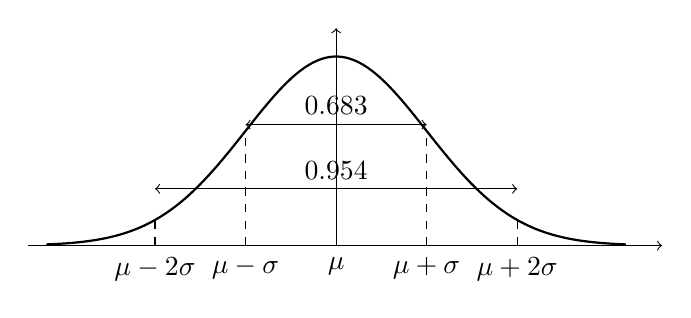
\begin{tikzpicture}[x=1.15cm,y=2.4cm]
  \draw[->] (-3.4,0) -- (3.6,0);
  \draw[->] (0,0) -- (0,1.15);
  \draw[thick,domain=-3.2:3.2,samples=120,smooth] plot (\x,{exp(-(\x*\x)/2)});
  \foreach \x in {-2,-1,1,2}
    \draw[dashed] (\x,0) -- (\x,{exp(-(\x*\x)/2)});
  \draw[dashed] (0,0) -- (0,1);
  \node[below] at (-2,-0.01) {$\mu-2\sigma$};
  \node[below] at (-1,-0.01) {$\mu-\sigma$};
  \node[below] at (0,-0.01) {$\mu$};
  \node[below] at (1,-0.01) {$\mu+\sigma$};
  \node[below] at (2,-0.01) {$\mu+2\sigma$};
  \draw[<->] (-1,0.64) -- (1,0.64) node[midway,above]{$0.683$};
  \draw[<->] (-2,0.30) -- (2,0.30) node[midway,above]{$0.954$};
\end{tikzpicture}
\phantomsection\label{fig:4.1}\mvcap{图 4.1\quad 具有均值 $\boldsymbol{\mu}$ 和方差 $\sigma^{2}$ 的正态密度及曲线下选定的面积}
\end{mvfigure}

用 $N(\mu,\sigma^{2})$ 表示具有均值 $\mu$ 和方差 $\sigma^{2}$ 的正态密度函数是方便的. 因此,$N(10,4)$ 表明\hyperref[eq:4-1]{式(4-1)}中的函数有 $\mu=10$ 和 $\sigma=2$. 这个表示法将扩展到以后的多元情况.

%% ===== pg-128 =====

在一元正态密度函数的指数中,以单位标准差测量从 $x$ 到 $\mu$ 的距离的平方
\phantomsection\label{eq:4-2}
\begin{equation}
\mvfit{$\displaystyle
\left(\frac{x-\mu}{\sigma}\right)^{2}=(x-\mu)(\sigma^{2})^{-1}(x-\mu)
$} \tag{4-2}
\end{equation}
这可以推广到根据关于若干个变量的观测结果的 $p\times1$ 向量 $\mathbf{x}$ 上,如
\phantomsection\label{eq:4-3}
\begin{equation}
\mvfit{$\displaystyle
(\mathbf{x}-\boldsymbol{\mu})'\boldsymbol{\Sigma}^{-1}(\mathbf{x}-\boldsymbol{\mu})
$} \tag{4-3}
\end{equation}
$p\times1$ 向量 $\boldsymbol{\mu}$ 表示随机向量 $\mathbf{X}$ 的期望值,$p\times p$ 矩阵 $\boldsymbol{\Sigma}$ 是 $\mathbf{X}$ 的方差-协方差矩阵[参见\hyperref[eq:2-30]{式(2-30)}和\hyperref[eq:2-31]{式(2-31)}]. 我们假定对称矩阵 $\boldsymbol{\Sigma}$ 是正定的,所以表达\hyperref[eq:4-3]{式(4-3)}是从 $\mathbf{x}$ 到 $\boldsymbol{\mu}$ 的广义距离的平方.

在\hyperref[eq:4-1]{式(4-1)}的密度函数中,用\hyperref[eq:4-3]{式(4-3)}的多元广义距离替换\hyperref[eq:4-2]{式(4-2)}中的一元距离,就得到多元正态密度. 当这个替换完成时,一元标准化常数 $(2\pi)^{-1/2}(\sigma^{2})^{-1/2}$ 必须变成一个更一般的常数,使得对任何 $p$,多元密度函数表面下的体积为 1. 这是必要的,因为在多元情况,概率是由 $x_i$ 值的区间定义的区域上方表面下的体积表示. 可以证明(参见文献[1])这个常数是 $(2\pi)^{-p/2}|\boldsymbol{\Sigma}|^{-1/2}$,因此,对随机向量 $\mathbf{X}=[X_1,X_2,\cdots,X_p]$,$p$ 维正态密度如下所示
\phantomsection\label{eq:4-4}
\begin{equation}
\mvfit{$\displaystyle
f(\mathbf{x})=\frac{1}{(2\pi)^{p/2}|\boldsymbol{\Sigma}|^{1/2}}\mathrm{e}^{-(\mathbf{x}-\boldsymbol{\mu})'\boldsymbol{\Sigma}^{-1}(\mathbf{x}-\boldsymbol{\mu})/2}
$} \tag{4-4}
\end{equation}
其中 $-\infty<x_i<\infty,i=1,2,\cdots,p$. 类似于一元情况的正态密度,我们用 $N_p(\boldsymbol{\mu},\boldsymbol{\Sigma})$ 表示 $p$ 维正态密度.

\noindent\textbf{例 4.1}\quad (二元正态密度)

根据参数 $\mu_1=E(X_1),\mu_2=E(X_2),\sigma_{11}=\operatorname{Var}(X_1),\sigma_{22}=\operatorname{Var}(X_2)$ 和 $\rho_{12}=\sigma_{12}/(\sqrt{\sigma_{11}}\sqrt{\sigma_{22}})=\operatorname{Corr}(X_1,X_2)$,计算 $p=2$ 元正态密度.

利用结论 2A.8,我们求得协方差矩阵
\[
\boldsymbol{\Sigma}=\begin{bmatrix}\sigma_{11}&\sigma_{12}\\\sigma_{12}&\sigma_{22}\end{bmatrix}
\]
的逆是
\[
\boldsymbol{\Sigma}^{-1}=\frac{1}{\sigma_{11}\sigma_{22}-\sigma_{12}^{2}}\begin{bmatrix}\sigma_{22}&-\sigma_{12}\\-\sigma_{12}&\sigma_{11}\end{bmatrix}
\]
由 $\sigma_{12}=\rho_{12}\sqrt{\sigma_{11}}\sqrt{\sigma_{22}}$,引入相关系数 $\rho_{12}$,我们得到 $\sigma_{11}\sigma_{22}-\sigma_{12}^{2}=\sigma_{11}\sigma_{22}(1-\rho_{12}^{2})$,且距离平方变为
\phantomsection\label{eq:4-5}
\begin{equation}
\mvfit{$\displaystyle\begin{aligned}
(\mathbf{x}-\boldsymbol{\mu})'\boldsymbol{\Sigma}^{-1}(\mathbf{x}-\boldsymbol{\mu})
&=[x_1-\mu_1,x_2-\mu_2]\frac{1}{\sigma_{11}\sigma_{22}(1-\rho_{12}^{2})}\begin{bmatrix}\sigma_{22}&-\rho_{12}\sqrt{\sigma_{11}}\sqrt{\sigma_{22}}\\-\rho_{12}\sqrt{\sigma_{11}}\sqrt{\sigma_{22}}&\sigma_{11}\end{bmatrix}\begin{bmatrix}x_1-\mu_1\\x_2-\mu_2\end{bmatrix}\\
&=\frac{\sigma_{22}(x_1-\mu_1)^{2}+\sigma_{11}(x_2-\mu_2)^{2}-2\rho_{12}\sqrt{\sigma_{11}}\sqrt{\sigma_{22}}(x_1-\mu_1)(x_2-\mu_2)}{\sigma_{11}\sigma_{22}(1-\rho_{12}^{2})}\\
&=\frac{1}{1-\rho_{12}^{2}}\left[\left(\frac{x_1-\mu_1}{\sqrt{\sigma_{11}}}\right)^{2}+\left(\frac{x_2-\mu_2}{\sqrt{\sigma_{22}}}\right)^{2}-2\rho_{12}\left(\frac{x_1-\mu_1}{\sqrt{\sigma_{11}}}\right)\left(\frac{x_2-\mu_2}{\sqrt{\sigma_{22}}}\right)\right]\end{aligned}$} \tag{4-5}
\end{equation}
最后表达式是依据标准化值 $(x_1-\mu_1)/\sqrt{\sigma_{11}}$ 和 $(x_2-\mu_2)/\sqrt{\sigma_{22}}$ 写出的.

接下来,由于 $|\boldsymbol{\Sigma}|=\sigma_{11}\sigma_{22}-\sigma_{12}^{2}=\sigma_{11}\sigma_{22}(1-\rho_{12}^{2})$,我们可以替换\hyperref[eq:4-4]{式(4-4)}中的 $\boldsymbol{\Sigma}^{-1}$ 和 $|\boldsymbol{\Sigma}|$ 而得到包含各个参数 $\mu_1,\mu_2,\sigma_{11},\sigma_{22}$ 和 $\rho_{12}$ 的二元($p=2$)正态密度:
\phantomsection\label{eq:4-6}
\begin{equation}
\mvfit{$\displaystyle
f(x_1,x_2)=\frac{1}{2\pi\sqrt{\sigma_{11}\sigma_{22}(1-\rho_{12}^{2})}}\exp\left\{-\frac{1}{2(1-\rho_{12}^{2})}\left[\left(\frac{x_1-\mu_1}{\sqrt{\sigma_{11}}}\right)^{2}+\left(\frac{x_2-\mu_2}{\sqrt{\sigma_{22}}}\right)^{2}-2\rho_{12}\left(\frac{x_1-\mu_1}{\sqrt{\sigma_{11}}}\right)\left(\frac{x_2-\mu_2}{\sqrt{\sigma_{22}}}\right)\right]\right\}
$} \tag{4-6}
\end{equation}

%% ===== pg-129 =====

\hyperref[eq:4-6]{式(4-6)}中的表达方法有点不便使用,而\hyperref[eq:4-4]{式(4-4)}中简洁通用的形式在许多方面提供信息更多. 另一方面,\hyperref[eq:4-6]{式(4-6)}中的表达方法对于讨论正态分布的某些性质是有用的. 例如,若随机向量 $X_1$ 和 $X_2$ 不相关,则 $\rho_{12}=0$,联合密度可以写作每个都如\hyperref[eq:4-1]{式(4-1)}所示的两个一元正态密度之积,即 $f(x_1,x_2)=f(x_1)f(x_2)$ 且 $X_1$ 和 $X_2$ 独立[参见\hyperref[eq:2-28]{式(2-28)}]. 该结论在一般情况下是正确的(参见结论 4.5).

$\sigma_{11}=\sigma_{22}$ 的两个二元正态分布如\hyperref[fig:4.2]{图 4.2} 所示. 在\hyperref[fig:4.2]{图 4.2}(a)中,$X_1$ 和 $X_2$ 是独立的($\rho_{12}=0$). 在\hyperref[fig:4.2]{图 4.2}(b)中,$\rho_{12}=0.75$. 注意,(b)中由于相关性的存在,促使概率沿一直线集中.

\begin{mvfigure}
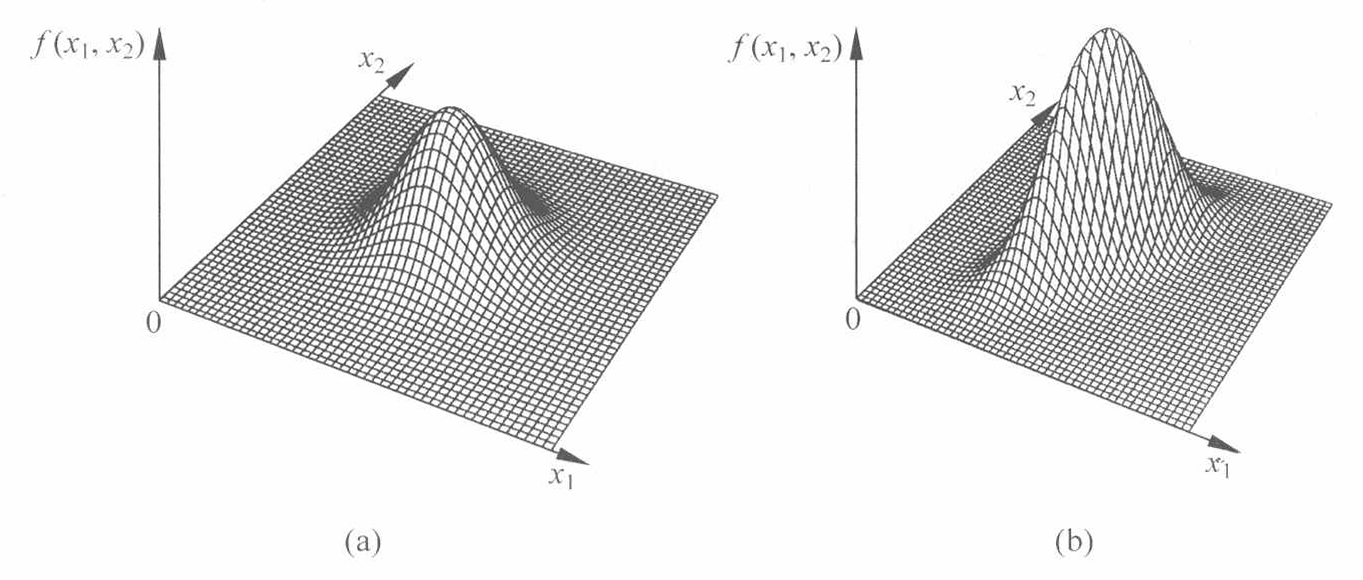
\includegraphics[width=115.4mm]{figs/fig_pg129_1.png}
\phantomsection\label{fig:4.2}\mvcap{图 4.2\quad 两个二元正态分布\\
(a) $\sigma_{11}=\sigma_{22}$ 且 $\rho_{12}=0$; (b) $\sigma_{11}=\sigma_{22}$ 且 $\rho_{12}=0.75$}
\end{mvfigure}

考虑一个 $p$ 维正态变量的密度,从\hyperref[eq:4-4]{式(4-4)}很清楚,对于密度产生一个常高的 $\mathbf{x}$ 值的路线为椭球面. 即在距离 $(\mathbf{x}-\boldsymbol{\mu})'\boldsymbol{\Sigma}^{-1}(\mathbf{x}-\boldsymbol{\mu})$ 的平方为常数的表面上多元正态密度是常数. 这些路线被称为轮廓线.

\begin{center}
常数概率密度轮廓线 $=\{$ 满足 $(\mathbf{x}-\boldsymbol{\mu})'\boldsymbol{\Sigma}^{-1}(\mathbf{x}-\boldsymbol{\mu})=c^{2}$ 的所有 $\mathbf{x}\}$\\
$=$ 中心在 $\boldsymbol{\mu}$ 的椭球的表面
\end{center}

常数密度的每个椭球面的轴在 $\boldsymbol{\Sigma}^{-1}$ 的特征向量的方向上,而且它们的长度是与 $\boldsymbol{\Sigma}^{-1}$ 的特征值的平方根的倒数成比例的. 幸运的是,当确定轴时,我们可以避免计算 $\boldsymbol{\Sigma}^{-1}$,因为这些椭球也是由 $\boldsymbol{\Sigma}$ 的特征值和特征向量所决定的. 为了以后参考方便,我们正式地陈述相应内容.

\mvthm{结论 4.1}{若 $\boldsymbol{\Sigma}$ 是正定的,于是 $\boldsymbol{\Sigma}^{-1}$ 存在,则
\[
\boldsymbol{\Sigma}\mathbf{e}=\lambda\mathbf{e}\quad\text{意味着}\quad \boldsymbol{\Sigma}^{-1}\mathbf{e}=\left(\frac{1}{\lambda}\right)\mathbf{e}
\]
所以 $(\lambda,\mathbf{e})$ 是 $\boldsymbol{\Sigma}$ 的一个特征值-特征向量对,对应于 $\boldsymbol{\Sigma}^{-1}$ 的特征值-特征向量对为 $(1/\lambda,\mathbf{e})$. 且 $\boldsymbol{\Sigma}^{-1}$ 也是正定的.}

\noindent\textbf{证明}\quad 对于 $\boldsymbol{\Sigma}$ 正定及一个特征向量 $\mathbf{e}\neq0$,我们有 $0<\mathbf{e}'\boldsymbol{\Sigma}\mathbf{e}=\mathbf{e}'(\boldsymbol{\Sigma}\mathbf{e})=\mathbf{e}'(\lambda\mathbf{e})=\lambda\mathbf{e}'\mathbf{e}=\lambda$. 而且 $\mathbf{e}=\boldsymbol{\Sigma}^{-1}(\boldsymbol{\Sigma}\mathbf{e})=\boldsymbol{\Sigma}^{-1}(\lambda\mathbf{e})$,或 $\mathbf{e}=\lambda\boldsymbol{\Sigma}^{-1}\mathbf{e}$,且用 $\lambda>0$ 除,得到 $\boldsymbol{\Sigma}^{-1}\mathbf{e}=(1/\lambda)\mathbf{e}$. 于是,$(1/\lambda,\mathbf{e})$ 是 $\boldsymbol{\Sigma}^{-1}$ 的一对特征值-特征向量. 又,对任何 $p\times1$ 的 $\mathbf{x}$,因为每项 $\lambda_i^{-1}(\mathbf{x}'\mathbf{e}_i)^{2}$ 是非负的,由\hyperref[eq:2-21]{式(2-21)},有

%% ===== pg-130 =====

\[
\mathbf{x}'\boldsymbol{\Sigma}^{-1}\mathbf{x}=\mathbf{x}'\left(\sum_{i=1}^{p}\left(\frac{1}{\lambda_i}\right)\mathbf{e}_i\mathbf{e}_i'\right)\mathbf{x}
=\sum_{i=1}^{p}\left(\frac{1}{\lambda_i}\right)(\mathbf{x}'\mathbf{e}_i)^{2}\geqslant 0
\]
而且,对所有 $i$,仅当 $\mathbf{x}=\mathbf{0}$ 时,$\mathbf{x}'\mathbf{e}_i=0$. 因此,$\mathbf{x}\neq\mathbf{0}$ 意味着 $\sum_{i=1}^{p}(1/\lambda_i)(\mathbf{x}'\mathbf{e}_i)^{2}>0$,由此得出 $\boldsymbol{\Sigma}^{-1}$ 是正定的.\hfill$\blacksquare$

这些概念可总结如下:

\begin{mvbox}
对 $p$ 维正态分布,常数密度的轮廓线是由 $\mathbf{x}$ 所确定的椭球面,满足
\phantomsection\label{eq:4-7}
\begin{equation}
(\mathbf{x}-\boldsymbol{\mu})'\boldsymbol{\Sigma}^{-1}(\mathbf{x}-\boldsymbol{\mu})=c^{2}
\tag{4-7}
\end{equation}
这些椭球面的中心在 $\boldsymbol{\mu}$ 且轴为 $\pm c\sqrt{\lambda_i}\mathbf{e}_i$,其中 $\boldsymbol{\Sigma}\mathbf{e}_i=\lambda_i\mathbf{e}_i$,对 $i=1,2,\cdots,p$.
\end{mvbox}

对 $\sigma_{11}=\sigma_{22}$ 的二元正态分布,下例求出常数密度的轮廓线.

\noindent\textbf{例 4.2}\quad (二元正态密度的轮廓线)

对二元正态分布,当 $\sigma_{11}=\sigma_{22}$ 时,我们将得到常数概率密度轮廓线的轴. 从\hyperref[eq:4-7]{式(4-7)},这些轴由 $\boldsymbol{\Sigma}$ 的特征值和特征向量给出. 这里 $|\boldsymbol{\Sigma}-\lambda\mathbf{I}|=0$ 变为
\begin{align*}
0&=\begin{vmatrix}\sigma_{11}-\lambda&\sigma_{12}\\\sigma_{12}&\sigma_{11}-\lambda\end{vmatrix}=(\sigma_{11}-\lambda)^{2}-\sigma_{12}^{2}\\
&=(\lambda-\sigma_{11}-\sigma_{12})(\lambda-\sigma_{11}+\sigma_{12})
\end{align*}
因此,特征值是 $\lambda_1=\sigma_{11}+\sigma_{12}$ 和 $\lambda_2=\sigma_{11}-\sigma_{12}$. 特征向量 $\mathbf{e}_1$ 是由
\[
\begin{bmatrix}\sigma_{11}&\sigma_{12}\\\sigma_{12}&\sigma_{11}\end{bmatrix}\begin{bmatrix}e_1\\e_2\end{bmatrix}=(\sigma_{11}+\sigma_{12})\begin{bmatrix}e_1\\e_2\end{bmatrix}
\]
或
\begin{align*}
\sigma_{11}e_1+\sigma_{12}e_2&=(\sigma_{11}+\sigma_{12})e_1\\
\sigma_{12}e_1+\sigma_{11}e_2&=(\sigma_{11}+\sigma_{12})e_2
\end{align*}
确定的. 这些等式意味着 $e_1=e_2$. 在标准化之后,第一对特征值-特征向量为
\[
\lambda_1=\sigma_{11}+\sigma_{12},\qquad \mathbf{e}_1=\begin{bmatrix}\dfrac{1}{\sqrt{2}}\\[2ex]\dfrac{1}{\sqrt{2}}\end{bmatrix}
\]
同样的,$\lambda_2=\sigma_{11}-\sigma_{12}$ 得出特征向量 $\mathbf{e}_2'=[1/\sqrt{2},-1/\sqrt{2}]$.

当协方差 $\sigma_{12}$(或相关系数 $\rho_{12}$)为正时,$\lambda_1=\sigma_{11}+\sigma_{12}$ 是最大特征值,它对应的特征向量 $\mathbf{e}_1'=[1/\sqrt{2},1/\sqrt{2}]$ 位于通过点 $\boldsymbol{\mu}'=[\mu_1,\mu_2]$ 的 $45^\circ$ 线上. 这对于协方差(相关系数)的任何正值都是正确的. 由于常数密度椭圆的轴是由 $\pm c\sqrt{\lambda_1}\mathbf{e}_1$ 和 $\pm c\sqrt{\lambda_2}\mathbf{e}_2$(参见\hyperref[eq:4-7]{式(4-7)})给出,且每个特征向量为单位长度,长轴将对应最大的特征值. 对于正相关正态随机变量,则常数密度椭圆的长轴是在通过 $\boldsymbol{\mu}$ 点的 $45^\circ$ 线上(参见\hyperref[fig:4.3]{图 4.3}). 当协方差(相关系数)是负值时,$\lambda_2=\sigma_{11}-\sigma_{12}$ 是最大的特征值,且常数密度椭圆的长轴在与过 $\boldsymbol{\mu}$ 点的 $45^\circ$ 线相垂直的线上(这些结论仅对 $\sigma_{11}=\sigma_{22}$ 是正确的).

总之,对于 $\sigma_{11}=\sigma_{22}$ 的二元正态分布,常数密度椭圆的轴由下式确定

%% ===== pg-131 =====

\[
\pm c\sqrt{\sigma_{11}+\sigma_{12}}\begin{bmatrix}\dfrac{1}{\sqrt{2}}\\[2ex]\dfrac{1}{\sqrt{2}}\end{bmatrix}
\quad\text{和}\quad
\pm c\sqrt{\sigma_{11}-\sigma_{12}}\begin{bmatrix}\dfrac{1}{\sqrt{2}}\\[2ex]-\dfrac{1}{\sqrt{2}}\end{bmatrix}
\]
\hfill$\blacksquare$

我们指出在结论 4.7 中,选择 $c^{2}=\chi_p^{2}(\alpha)$,这里 $\chi_p^{2}(\alpha)$ 是自由度为 $p$ 的 $\chi^{2}$ 分布的上 $(100\alpha)$ 百分位数,将导致含概率 $(1-\alpha)100\%$ 的轮廓线. 特别对 $p$ 维正态分布,以下命题是正确的:

\begin{mvbox}
满足
\phantomsection\label{eq:4-8}
\begin{equation}
(\mathbf{x}-\boldsymbol{\mu})'\boldsymbol{\Sigma}^{-1}(\mathbf{x}-\boldsymbol{\mu})\leqslant\chi_p^{2}(\alpha)
\tag{4-8}
\end{equation}
的 $\mathbf{x}$ 值的实心椭球有概率 $1-\alpha$.
\end{mvbox}

\hyperref[fig:4.2]{图 4.2} 中的二元正态分布的概率 $50\%$ 和 $90\%$ 的常数密度轮廓线如\hyperref[fig:4.4]{图 4.4} 所示.

\begin{mvfigure}
\begin{minipage}{0.48\linewidth}\centering
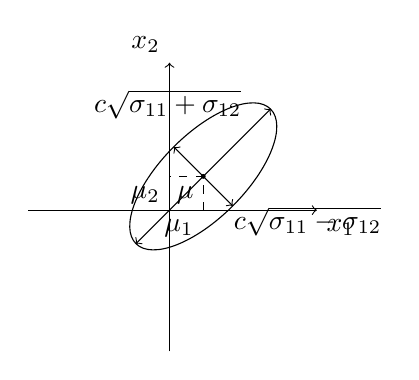
\begin{tikzpicture}[scale=0.78]
  \draw[->] (-2.3,0) -- (2.4,0) node[below right]{$x_1$};
  \draw[->] (0,-2.3) -- (0,2.4) node[above left]{$x_2$};
  \coordinate (m) at (0.55,0.55);
  \draw[dashed] (0.55,0) -- (0.55,0.55) -- (0,0.55);
  \fill (0.55,0.55) circle (0.04);
  \node[below left] at (0.55,0.55) {$\mu$};
  \node[below left] at (0.55,0) {$\mu_1$};
  \node[below left] at (0,0.55) {$\mu_2$};
  \draw[rotate around={45:(0.55,0.55)}] (0.55,0.55) ellipse (1.55 and 0.68);
  \draw[<->] (0.55-1.10,0.55-1.10) -- (0.55+1.10,0.55+1.10);
  \node[above left] at (0.55+0.78,0.55+0.78) {$c\sqrt{\sigma_{11}+\sigma_{12}}$};
  \draw[<->] (0.55-0.48,0.55+0.48) -- (0.55+0.48,0.55-0.48);
  \node[below right] at (0.55+0.34,0.55-0.34) {$c\sqrt{\sigma_{11}-\sigma_{12}}$};
\end{tikzpicture}
\phantomsection\label{fig:4.3}\mvcap{图 4.3\quad 对于 $\sigma_{11}=\sigma_{22}$ 且 $\sigma_{12}>0$(或 $\rho_{12}>0$)的\\ 二元正态分布的常数密度轮廓线}
\end{minipage}\hfill
\begin{minipage}{0.48\linewidth}\centering
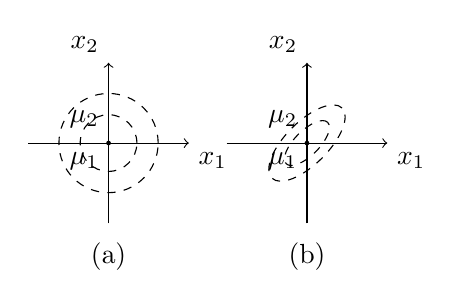
\begin{tikzpicture}[scale=0.6]
  \begin{scope}
    \draw[->] (-1.7,0) -- (1.7,0) node[below right]{$x_1$};
    \draw[->] (0,-1.7) -- (0,1.7) node[above left]{$x_2$};
    \draw[dashed] (0,0) circle (0.6);
    \draw[dashed] (0,0) circle (1.05);
    \draw[dashed] (0,-0.05) -- (0,0);
    \fill (0,0) circle (0.05);
    \node[below left] at (0,0) {$\mu_1$};
    \node[below left] at (0,0.9) {$\mu_2$};
    \node[below] at (0,-1.9) {(a)};
  \end{scope}
  \begin{scope}[xshift=4.2cm]
    \draw[->] (-1.7,0) -- (1.7,0) node[below right]{$x_1$};
    \draw[->] (0,-1.7) -- (0,1.7) node[above left]{$x_2$};
    \draw[dashed,rotate around={45:(0,0)}] (0,0) ellipse (1.05 and 0.45);
    \draw[dashed,rotate around={45:(0,0)}] (0,0) ellipse (0.62 and 0.26);
    \fill (0,0) circle (0.05);
    \node[below left] at (0,0) {$\mu_1$};
    \node[below left] at (0,0.9) {$\mu_2$};
    \node[below] at (0,-1.9) {(b)};
  \end{scope}
\end{tikzpicture}
\phantomsection\label{fig:4.4}\mvcap{图 4.4\quad \hyperref[fig:4.2]{图 4.2} 中的二元正态分布的概率 $50\%$ 和\\ $90\%$ 的常数密度轮廓线}
\end{minipage}
\end{mvfigure}

当\hyperref[eq:4-3]{式(4-3)}中的距离平方是零——即当 $\mathbf{x}=\boldsymbol{\mu}$ 时,\hyperref[eq:4-4]{式(4-4)}中的 $p$ 元正态密度有最大值. 因此,$\boldsymbol{\mu}$ 是密度最大的点,或众数,也是 $\mathbf{X}$ 的期望值(或均值). $\boldsymbol{\mu}$ 为多元正态分布的均值,这是由常数密度轮廓线所显示的对称性得出的:这些轮廓线中心在 $\boldsymbol{\mu}$ 或对称于 $\boldsymbol{\mu}$.

\mvsub{多元正态分布的可加性}

在我们对于统计模型和方法的解释中,必须重复正态分布的一些性质. 这些性质使我们有可能轻松熟练地使用正态分布,并且正如我们在 4.1 节所指出的,这些性质对正态分布的广泛运用起到了一部分作用. 我们可以相当简洁地陈述主要性质,并很快从数学角度详细讨论.

对于具有多元正态分布的随机向量 $\mathbf{X}$,下列性质是正确的:

1. $\mathbf{X}$ 的分量的线性组合是正态分布.

2. $\mathbf{X}$ 的分量的所有的子集有一个(多元)正态分布.

3. 零协方差意味着相应的分量是独立分布的.

4. 分量的条件分布是(多元)正态的.

这些性质在下面的结论中用数学方法重新表述. 这些结论中的多数用例题来说明. 所给出的证明有助于提高对矩阵运算的理解,并且促进对这些结论相继建立的方式的认识.

结论 4.2 可以用来作为正态分布的一个实用的定义. 采用该定义,以后的性质几乎可以直接得到. 结论 4.2 的部分的证明指出,一个正态密度的线性组合定义如何与\hyperref[eq:4-4]{式(4-4)}中的多元密度相联系.

\mvthm{结论 4.2}{若 $\mathbf{X}$ 的分布为 $N_p(\boldsymbol{\mu},\boldsymbol{\Sigma})$,则多个变量的任何线性组合 $\mathbf{a}'\mathbf{X}=a_1X_1+a_2X_2+\cdots+$}

%% ===== pg-132 =====

$a_pX_p$ 服从 $N(\mathbf{a}'\boldsymbol{\mu},\mathbf{a}'\boldsymbol{\Sigma}\mathbf{a})$ 分布. 而且,对每个 $\mathbf{a}$,若 $\mathbf{a}'\mathbf{X}$ 服从 $N(\mathbf{a}'\boldsymbol{\mu},\mathbf{a}'\boldsymbol{\Sigma}\mathbf{a})$ 分布,则 $\mathbf{X}$ 必须是 $N_p(\boldsymbol{\mu},\boldsymbol{\Sigma})$.

\noindent\textbf{证明}\quad 从\hyperref[eq:2-43]{式(2-43)}得出 $\mathbf{a}'\mathbf{X}$ 的期望值和方差. 若 $\mathbf{X}$ 是多元正态的,证明 $\mathbf{a}'\mathbf{X}$ 是正态分布会很困难. 可以在文献[1]中找到证明. 结论 4.2 的第二部分也在文献[1]中有证明.\hfill$\blacksquare$

\noindent\textbf{例 4.3}\quad (正态随机向量的分量的一个线性组合的分布)

考虑由选择 $\mathbf{a}'=[1,0,\cdots,0]$ 所确定的多元正态随机向量的线性组合 $\mathbf{a}'\mathbf{X}$,由于
\[
\mathbf{a}'\mathbf{X}=[1,0,\cdots,0]\begin{bmatrix}X_1\\X_2\\\vdots\\X_p\end{bmatrix}=X_1
\]
和
\[
\mathbf{a}'\boldsymbol{\mu}=[1,0,\cdots,0]\begin{bmatrix}\mu_1\\\mu_2\\\vdots\\\mu_p\end{bmatrix}=\mu_1
\]
我们有
\[
\mathbf{a}'\boldsymbol{\Sigma}\mathbf{a}=[1,0,\cdots,0]\begin{bmatrix}\sigma_{11}&\sigma_{12}&\cdots&\sigma_{1p}\\\sigma_{12}&\sigma_{22}&\cdots&\sigma_{2p}\\\vdots&\vdots&&\vdots\\\sigma_{1p}&\sigma_{2p}&\cdots&\sigma_{pp}\end{bmatrix}\begin{bmatrix}1\\0\\\vdots\\0\end{bmatrix}=\sigma_{11}
\]
且从结论 4.2 得出的 $X_1$ 服从 $N(\mu_1,\sigma_{11})$ 分布. 更一般的,$\mathbf{X}$ 的任何分量 $X_i$ 的边缘分布是 $N(\mu_i,\sigma_{ii})$.\hfill$\blacksquare$

下面的结论考虑一个多元正态向量 $\mathbf{X}$ 的若干个线性组合.

\mvthm{结论 4.3}{如果 $\mathbf{X}$ 服从 $N_p(\boldsymbol{\mu},\boldsymbol{\Sigma})$ 分布,$q$ 个线性组合
\[
\underset{(q\times p)}{\mathbf{A}}\mathbf{X}=\begin{bmatrix}a_{11}X_1+\cdots+a_{1p}X_p\\a_{21}X_1+\cdots+a_{2p}X_p\\\vdots\\a_{q1}X_1+\cdots+a_{qp}X_p\end{bmatrix}
\]
服从 $N_q(\mathbf{A}\boldsymbol{\mu},\mathbf{A}\boldsymbol{\Sigma}\mathbf{A}')$ 分布. 又,$\mathbf{X}+\mathbf{d}$ 服从 $N_p(\boldsymbol{\mu}+\mathbf{d},\boldsymbol{\Sigma})$ 分布,其中 $\mathbf{d}$ 为常数向量.}

\noindent\textbf{证明}\quad 从\hyperref[eq:2-45]{式(2-45)}得出 $\mathbf{A}\mathbf{X}$ 的期望值 $E(\mathbf{A}\mathbf{X})$ 和协方差矩阵. 任何线性组合 $\mathbf{b}'(\mathbf{A}\mathbf{X})$ 是 $\mathbf{X}$ 的形如 $\mathbf{a}'\mathbf{X}$ 的一个线性组合,其中 $\mathbf{a}=\mathbf{A}'\mathbf{b}$. 于是,从结论 4.2 直接得出关于 $\mathbf{A}\mathbf{X}$ 的最后结论.

结论的第二部分通过考察 $\mathbf{a}'(\mathbf{X}+\mathbf{d})=\mathbf{a}'\mathbf{X}+(\mathbf{a}'\mathbf{d})$ 可以得到,其中 $\mathbf{a}'\mathbf{X}$ 服从 $N(\mathbf{a}'\boldsymbol{\mu},\mathbf{a}'\boldsymbol{\Sigma}\mathbf{a})$ 分布. 从一元情况可知,加一个常数 $\mathbf{a}'\mathbf{d}$ 到随机变量 $\mathbf{a}'\mathbf{X}$ 上,方差不会变化,而均值变为 $\mathbf{a}'\boldsymbol{\mu}+\mathbf{a}'\mathbf{d}=\mathbf{a}'(\boldsymbol{\mu}+\mathbf{d})$. 由于 $\mathbf{a}$ 是任意的,$\mathbf{X}+\mathbf{d}$ 服从 $N_p(\boldsymbol{\mu}+\mathbf{d},\boldsymbol{\Sigma})$ 分布.\hfill$\blacksquare$

\noindent\textbf{例 4.4}\quad (正态随机向量的分量的两个线性组合的分布)

考虑 $\mathbf{X}$ 服从 $N_3(\boldsymbol{\mu},\boldsymbol{\Sigma})$ 分布,求
\[
\begin{bmatrix}X_1-X_2\\X_2-X_3\end{bmatrix}=\begin{bmatrix}1&-1&0\\0&1&-1\end{bmatrix}\begin{bmatrix}X_1\\X_2\\X_3\end{bmatrix}=\mathbf{A}\mathbf{X}
\]

%% ===== pg-133 =====

的分布.

由结论 4.3,$\mathbf{A}\mathbf{X}$ 的分布为多元正态,其均值为
\[
\mathbf{A}\boldsymbol{\mu}=\begin{bmatrix}1&-1&0\\0&1&-1\end{bmatrix}\begin{bmatrix}\mu_1\\\mu_2\\\mu_3\end{bmatrix}=\begin{bmatrix}\mu_1-\mu_2\\\mu_2-\mu_3\end{bmatrix}
\]
协方差矩阵为
\begin{align*}
\mathbf{A}\boldsymbol{\Sigma}\mathbf{A}'&=\begin{bmatrix}1&-1&0\\0&1&-1\end{bmatrix}\begin{bmatrix}\sigma_{11}&\sigma_{12}&\sigma_{13}\\\sigma_{12}&\sigma_{22}&\sigma_{23}\\\sigma_{13}&\sigma_{23}&\sigma_{33}\end{bmatrix}\begin{bmatrix}1&0\\-1&1\\0&-1\end{bmatrix}\\
&=\begin{bmatrix}\sigma_{11}-\sigma_{12}&\sigma_{12}-\sigma_{22}&\sigma_{13}-\sigma_{23}\\\sigma_{12}-\sigma_{13}&\sigma_{22}-\sigma_{23}&\sigma_{23}-\sigma_{33}\end{bmatrix}\begin{bmatrix}1&0\\-1&1\\0&-1\end{bmatrix}\\
&=\begin{bmatrix}\sigma_{11}-2\sigma_{12}+\sigma_{22}&\sigma_{12}+\sigma_{13}-\sigma_{22}-\sigma_{23}\\\sigma_{12}+\sigma_{13}-\sigma_{22}-\sigma_{23}&\sigma_{22}-2\sigma_{23}+\sigma_{33}\end{bmatrix}
\end{align*}
换言之,通过直接计算两个随机变量 $Y_1=X_1-X_2$ 和 $Y_2=X_2-X_3$ 的均值和协方差,可以验证均值向量 $\mathbf{A}\boldsymbol{\mu}$ 和协方差矩阵 $\mathbf{A}\boldsymbol{\Sigma}\mathbf{A}'$.\hfill$\blacksquare$

我们提到过一个多元正态随机向量 $\mathbf{X}$ 的所有子集本身是正态的. 在结论 4.4 中我们正式地描述这一性质.

\mvthm{结论 4.4}{$\mathbf{X}$ 的所有子集是正态分布. 若我们分别把 $\mathbf{X}$ 及其均值向量 $\boldsymbol{\mu}$ 和协方差矩阵 $\boldsymbol{\Sigma}$ 划分为
\[
\underset{(p\times1)}{\mathbf{X}}=\begin{bmatrix}\underset{(q\times1)}{\mathbf{X}_1}\\[2ex]\underset{((p-q)\times1)}{\mathbf{X}_2}\end{bmatrix},\qquad
\underset{(p\times1)}{\boldsymbol{\mu}}=\begin{bmatrix}\underset{(q\times1)}{\boldsymbol{\mu}_1}\\[2ex]\underset{((p-q)\times1)}{\boldsymbol{\mu}_2}\end{bmatrix}
\]
和
\[
\underset{(p\times p)}{\boldsymbol{\Sigma}}=\left[\begin{array}{c|c}
\underset{(q\times q)}{\boldsymbol{\Sigma}_{11}}&\underset{(q\times(p-q))}{\boldsymbol{\Sigma}_{12}}\\
\hdashline
\underset{((p-q)\times q)}{\boldsymbol{\Sigma}_{21}}&\underset{((p-q)\times(p-q))}{\boldsymbol{\Sigma}_{22}}
\end{array}\right]
\]
则 $\mathbf{X}_1$ 服从 $N_q(\boldsymbol{\mu}_1,\boldsymbol{\Sigma}_{11})$ 分布.}

\noindent\textbf{证明}\quad 令结论 4.3 中的 $\mathbf{A}=\left[\underset{(q\times q)}{\mathbf{I}}\quad\underset{(q\times(p-q))}{\mathbf{0}}\right]$,结论成立. 至于把结论 4.4 应用于 $\mathbf{X}$ 的分量的任意子集,我们只需把感兴趣的子集重新标为 $\mathbf{X}_1$,并分别选择相应的均值和协方差分量为 $\boldsymbol{\mu}_1$ 和 $\boldsymbol{\Sigma}_{11}$.\hfill$\blacksquare$

\noindent\textbf{例 4.5}\quad (正态随机向量的子集的分布)

若 $\mathbf{X}$ 服从 $N_3(\boldsymbol{\mu},\boldsymbol{\Sigma})$ 分布,求 $\begin{bmatrix}X_2\\X_1\end{bmatrix}$ 的分布.

设
\[
\mathbf{X}_1=\begin{bmatrix}X_2\\X_1\end{bmatrix},\qquad \boldsymbol{\mu}=\begin{bmatrix}\mu_2\\\mu_1\end{bmatrix},\qquad \boldsymbol{\Sigma}_{11}=\begin{bmatrix}\sigma_{22}&\sigma_{21}\\\sigma_{21}&\sigma_{11}\end{bmatrix}
\]
且注意到,在该分布下,$\mathbf{X},\boldsymbol{\mu}$ 和 $\boldsymbol{\Sigma}$ 分别可以重新排列和划分为

%% ===== pg-134 =====

\[
\mathbf{X}=\begin{bmatrix}X_2\\X_4\\X_1\\X_3\\X_5\end{bmatrix},\qquad
\boldsymbol{\mu}=\begin{bmatrix}\mu_2\\\mu_4\\\mu_1\\\mu_3\\\mu_5\end{bmatrix},\qquad
\boldsymbol{\Sigma}=\begin{bmatrix}\sigma_{22}&\sigma_{24}&\sigma_{12}&\sigma_{23}&\sigma_{25}\\\sigma_{24}&\sigma_{44}&\sigma_{14}&\sigma_{34}&\sigma_{45}\\\sigma_{12}&\sigma_{14}&\sigma_{11}&\sigma_{13}&\sigma_{15}\\\sigma_{23}&\sigma_{34}&\sigma_{13}&\sigma_{33}&\sigma_{35}\\\sigma_{25}&\sigma_{45}&\sigma_{15}&\sigma_{35}&\sigma_{55}\end{bmatrix}
\]
或
\[
\mathbf{X}=\begin{bmatrix}\underset{(2\times1)}{\mathbf{X}_1}\\[2ex]\underset{(3\times1)}{\mathbf{X}_2}\end{bmatrix},\qquad
\boldsymbol{\mu}=\begin{bmatrix}\underset{(2\times1)}{\boldsymbol{\mu}_1}\\[2ex]\underset{(3\times1)}{\boldsymbol{\mu}_2}\end{bmatrix},\qquad
\boldsymbol{\Sigma}=\begin{bmatrix}\underset{(2\times2)}{\boldsymbol{\Sigma}_{11}}&\underset{(2\times3)}{\boldsymbol{\Sigma}_{12}}\\[2ex]\underset{(3\times2)}{\boldsymbol{\Sigma}_{21}}&\underset{(3\times3)}{\boldsymbol{\Sigma}_{22}}\end{bmatrix}
\]
于是,从结论 4.4,对于
\[
\mathbf{X}_1=\begin{bmatrix}X_2\\X_4\end{bmatrix}
\]
我们有分布
\[
N_2(\boldsymbol{\mu}_1,\boldsymbol{\Sigma}_{11})=N_2\left(\begin{bmatrix}\mu_2\\\mu_4\end{bmatrix},\begin{bmatrix}\sigma_{22}&\sigma_{24}\\\sigma_{24}&\sigma_{44}\end{bmatrix}\right)
\]
从本例可清楚看出,对于任何子集正态分布可以通过仅仅从原来的 $\boldsymbol{\mu}$ 和 $\boldsymbol{\Sigma}$ 选择适当的均值和协方差来表示. 形式上的重新标号和划分的过程是多余的.\hfill$\blacksquare$

现在我们能够指出,正态随机变量之间或正态随机变量的集合之间的零相关与统计独立是等价的.

\mvthm{结论 4.5}{(a) 若 $\underset{(q_1\times1)}{\mathbf{X}_1}$ 和 $\underset{(q_2\times1)}{\mathbf{X}_2}$ 独立,则 $\operatorname{Cov}(\mathbf{X}_1,\mathbf{X}_2)=\mathbf{0}$,即一个 $q_1\times q_2$ 的零矩阵.

(b) 若 $\begin{bmatrix}\mathbf{X}_1\\\mathbf{X}_2\end{bmatrix}$ 为 $N_{q_1+q_2}\left(\begin{bmatrix}\boldsymbol{\mu}_1\\\boldsymbol{\mu}_2\end{bmatrix},\begin{bmatrix}\boldsymbol{\Sigma}_{11}&\boldsymbol{\Sigma}_{12}\\\boldsymbol{\Sigma}_{21}&\boldsymbol{\Sigma}_{22}\end{bmatrix}\right)$,则当且仅当 $\boldsymbol{\Sigma}_{12}=\mathbf{0}$ 时,$\mathbf{X}_1$ 和 $\mathbf{X}_2$ 独立.

(c) 若 $\mathbf{X}_1$ 和 $\mathbf{X}_2$ 独立且分别服从 $N_{q_1}(\boldsymbol{\mu}_1,\boldsymbol{\Sigma}_{11})$ 分布和 $N_{q_2}(\boldsymbol{\mu}_2,\boldsymbol{\Sigma}_{22})$ 分布,则 $\begin{bmatrix}\mathbf{X}_1\\\mathbf{X}_2\end{bmatrix}$ 为多元正态分布
\[
N_{q_1+q_2}\left(\begin{bmatrix}\boldsymbol{\mu}_1\\\boldsymbol{\mu}_2\end{bmatrix},\begin{bmatrix}\boldsymbol{\Sigma}_{11}&\mathbf{0}\\\mathbf{0}'&\boldsymbol{\Sigma}_{22}\end{bmatrix}\right)
\]}

\noindent\textbf{证明}\quad (当 $\boldsymbol{\Sigma}_{12}=\mathbf{0}$ 时,部分证明根据密度函数的因式分解,参见练习 4.14.)\hfill$\blacksquare$

\noindent\textbf{例 4.6}\quad (对于正态变量,零协方差与独立性等价)

设 $\underset{(3\times1)}{\mathbf{X}}$ 为 $N_3(\boldsymbol{\mu},\boldsymbol{\Sigma})$,其中
\[
\boldsymbol{\Sigma}=\begin{bmatrix}4&1&0\\1&3&0\\0&0&2\end{bmatrix}
\]
$X_1$ 和 $X_3$ 是否独立? $(X_1,X_2)$ 和 $X_3$ 是否独立?

因为 $X_1$ 和 $X_2$ 的协方差 $\sigma_{12}=1$,它们不是独立的. 然而,$\mathbf{X}$ 和 $\boldsymbol{\Sigma}$ 划分为
\[
\mathbf{X}=\begin{bmatrix}X_1\\X_2\\X_3\end{bmatrix},\qquad
\boldsymbol{\Sigma}=\begin{bmatrix}4&1&0\\1&3&0\\0&0&2\end{bmatrix}=\begin{bmatrix}\underset{(2\times2)}{\boldsymbol{\Sigma}_{11}}&\underset{(2\times1)}{\boldsymbol{\Sigma}_{12}}\\\underset{(1\times2)}{\boldsymbol{\Sigma}_{21}}&\underset{(1\times1)}{\boldsymbol{\Sigma}_{22}}\end{bmatrix}
\]

%% ===== pg-135 =====

我们看到 $\mathbf{X}_1=\begin{bmatrix}X_1\\X_2\end{bmatrix}$ 和 $X_3$ 的协方差矩阵 $\boldsymbol{\Sigma}_{12}=\begin{bmatrix}0\\0\end{bmatrix}$。因此，$(X_1,X_2)$ 和 $X_3$ 根据结论 4.5 是独立的。这意味着 $X_3$ 对 $X_1$ 独立，对 $X_2$ 也独立。\hfill$\blacksquare$

在二元正态分布的讨论中，我们已指出 $\rho_{12}=0$（零相关）意味着独立，这是因为联合密度函数[参见\hyperref[eq:4-6]{式(4-6)}]可写成 $X_1$ 和 $X_2$ 的边缘（正态）密度之积。这种情况，只不过是结论 4.5 在 $q_1=q_2=1$ 时的一个特例，这一点可以直接证明。

\mvthm{结论 4.6}{设 $\mathbf{X}=\begin{bmatrix}\mathbf{X}_1\\\mathbf{X}_2\end{bmatrix}$ 是服从 $N_p(\boldsymbol{\mu},\boldsymbol{\Sigma})$ 的分布，$\boldsymbol{\mu}=\begin{bmatrix}\boldsymbol{\mu}_1\\\boldsymbol{\mu}_2\end{bmatrix}$，$\boldsymbol{\Sigma}=\begin{bmatrix}\boldsymbol{\Sigma}_{11}&\boldsymbol{\Sigma}_{12}\\\boldsymbol{\Sigma}_{21}&\boldsymbol{\Sigma}_{22}\end{bmatrix}$，且 $|\boldsymbol{\Sigma}_{22}|>0$。}

则给定 $\mathbf{X}_2=\mathbf{x}_2$ 时，$\mathbf{X}_1$ 的条件分布是正态的，并且

\[
\text{均值}=\boldsymbol{\mu}_1+\boldsymbol{\Sigma}_{12}\boldsymbol{\Sigma}_{22}^{-1}(\mathbf{x}_2-\boldsymbol{\mu}_2)
\]

和

\[
\text{协方差}=\boldsymbol{\Sigma}_{11}-\boldsymbol{\Sigma}_{12}\boldsymbol{\Sigma}_{22}^{-1}\boldsymbol{\Sigma}_{21}
\]

注意协方差不取决于条件变量的值 $\mathbf{x}_2$。

\noindent\textbf{证明}\quad 我们将给出一个间接的证明（参见练习 4.13，其中直接利用密度）。取

\[
A=\begin{bmatrix}
I_{q_1\times q_1} & -\boldsymbol{\Sigma}_{12}\boldsymbol{\Sigma}_{22}^{-1}\\[2pt]
\mathbf{0}_{(p-q_1)\times q_1} & I_{(p-q_1)\times(p-q_1)}
\end{bmatrix}
\]

于是

\[
A(\mathbf{X}-\boldsymbol{\mu})=A\begin{bmatrix}\mathbf{X}_1-\boldsymbol{\mu}_1\\\mathbf{X}_2-\boldsymbol{\mu}_2\end{bmatrix}
=\begin{bmatrix}
\mathbf{X}_1-\boldsymbol{\mu}_1-\boldsymbol{\Sigma}_{12}\boldsymbol{\Sigma}_{22}^{-1}(\mathbf{X}_2-\boldsymbol{\mu}_2)\\[2pt]
\mathbf{X}_2-\boldsymbol{\mu}_2
\end{bmatrix}
\]

是联合正态的，协方差矩阵 $A\boldsymbol{\Sigma}A'$ 由

\[
\begin{bmatrix}
I & -\boldsymbol{\Sigma}_{12}\boldsymbol{\Sigma}_{22}^{-1}\\
\mathbf{0} & I
\end{bmatrix}
\begin{bmatrix}
\boldsymbol{\Sigma}_{11} & \boldsymbol{\Sigma}_{12}\\
\boldsymbol{\Sigma}_{21} & \boldsymbol{\Sigma}_{22}
\end{bmatrix}
\begin{bmatrix}
I & \mathbf{0}\\
(-\boldsymbol{\Sigma}_{12}\boldsymbol{\Sigma}_{22}^{-1})' & I
\end{bmatrix}
=\begin{bmatrix}
\boldsymbol{\Sigma}_{11}-\boldsymbol{\Sigma}_{12}\boldsymbol{\Sigma}_{22}^{-1}\boldsymbol{\Sigma}_{21} & \mathbf{0}\\
\mathbf{0} & \boldsymbol{\Sigma}_{22}
\end{bmatrix}
\]

给出。

由于 $\mathbf{X}_1-\boldsymbol{\mu}_1-\boldsymbol{\Sigma}_{12}\boldsymbol{\Sigma}_{22}^{-1}(\mathbf{X}_2-\boldsymbol{\mu}_2)$ 与 $\mathbf{X}_2-\boldsymbol{\mu}_2$ 有零协方差，它们独立。而且，量 $\mathbf{X}_1-\boldsymbol{\mu}_1-\boldsymbol{\Sigma}_{12}\boldsymbol{\Sigma}_{22}^{-1}(\mathbf{X}_2-\boldsymbol{\mu}_2)$ 服从 $N_{q_1}(\mathbf{0},\boldsymbol{\Sigma}_{11}-\boldsymbol{\Sigma}_{12}\boldsymbol{\Sigma}_{22}^{-1}\boldsymbol{\Sigma}_{21})$ 分布。给定 $\mathbf{X}_2=\mathbf{x}_2$，$\boldsymbol{\mu}_1+\boldsymbol{\Sigma}_{12}\boldsymbol{\Sigma}_{22}^{-1}(\mathbf{x}_2-\boldsymbol{\mu}_2)$ 是一常数。因为 $\mathbf{X}_1-\boldsymbol{\mu}_1-\boldsymbol{\Sigma}_{12}\boldsymbol{\Sigma}_{22}^{-1}(\mathbf{X}_2-\boldsymbol{\mu}_2)$ 和 $\mathbf{X}_2-\boldsymbol{\mu}_2$ 独立，$\mathbf{X}_1-\boldsymbol{\mu}_1-\boldsymbol{\Sigma}_{12}\boldsymbol{\Sigma}_{22}^{-1}(\mathbf{X}_2-\boldsymbol{\mu}_2)$ 的条件分布与 $\mathbf{X}_1-\boldsymbol{\mu}_1-\boldsymbol{\Sigma}_{12}\boldsymbol{\Sigma}_{22}^{-1}(\mathbf{X}_2-\boldsymbol{\mu}_2)$ 的无条件分布是相同的。由于 $\mathbf{X}_1-\boldsymbol{\mu}_1-\boldsymbol{\Sigma}_{12}\boldsymbol{\Sigma}_{22}^{-1}(\mathbf{X}_2-\boldsymbol{\mu}_2)$ 服从 $N_{q_1}(\mathbf{0},\boldsymbol{\Sigma}_{11}-\boldsymbol{\Sigma}_{12}\boldsymbol{\Sigma}_{22}^{-1}\boldsymbol{\Sigma}_{21})$ 分布，因此，当 $\mathbf{X}_2$ 有特定值 $\mathbf{x}_2$ 时，随机向量 $\mathbf{X}_1-\boldsymbol{\mu}_1-\boldsymbol{\Sigma}_{12}\boldsymbol{\Sigma}_{22}^{-1}(\mathbf{x}_2-\boldsymbol{\mu}_2)$ 也是同一分布。等价地，给定 $\mathbf{X}_2=\mathbf{x}_2$ 时，$\mathbf{X}_1$ 服从 $N_{q_1}(\boldsymbol{\mu}_1+\boldsymbol{\Sigma}_{12}\boldsymbol{\Sigma}_{22}^{-1}(\mathbf{x}_2-\boldsymbol{\mu}_2),\boldsymbol{\Sigma}_{11}-\boldsymbol{\Sigma}_{12}\boldsymbol{\Sigma}_{22}^{-1}\boldsymbol{\Sigma}_{21})$ 分布。\hfill$\blacksquare$

\noindent\textbf{例 4.7}\quad （二元正态分布的条件密度）

对任何二元分布，在给定 $X_2=x_2$ 时，$X_1$ 的条件密度被定义为

\[
f(x_1\mid x_2)=\{\text{给定 }X_2=x_2,\ X_1 \text{ 的条件密度}\}=\frac{f(x_1,x_2)}{f_2(x_2)}
\]

其中 $f_2(x_2)$ 是 $X_2$ 的边缘分布。若 $f(x_1,x_2)$ 是二元正态密度，证明 $f(x_1\mid x_2)$ 为

\[
N\left(\mu_1+\frac{\sigma_{12}}{\sigma_{22}}(x_2-\mu_2),\ \sigma_{11}-\frac{\sigma_{12}^2}{\sigma_{22}}\right)
\]

这里 $\sigma_{11}-\sigma_{12}^2/\sigma_{22}=\sigma_{11}(1-\rho_{12}^2)$。在二元正态密度[参见\hyperref[eq:4-6]{式(4-6)}]的指数中，除去相乘的常数 $-1/2(1-\rho_{12}^2)$ 以外，包含 $x_1-\mu_1$ 的两项变成

%% ===== pg-136 =====

\[
\frac{(x_1-\mu_1)^2}{\sigma_{11}}-2\rho_{12}\frac{(x_1-\mu_1)(x_2-\mu_2)}{\sqrt{\sigma_{11}}\sqrt{\sigma_{22}}}
=\frac{1}{\sigma_{11}}\left[x_1-\mu_1-\rho_{12}\frac{\sqrt{\sigma_{11}}}{\sqrt{\sigma_{22}}}(x_2-\mu_2)\right]^2-\frac{\rho_{12}^2}{\sigma_{22}}(x_2-\mu_2)^2
\]

由于 $\rho_{12}=\sigma_{12}/\sqrt{\sigma_{11}}\sqrt{\sigma_{22}}$ 或 $\rho_{12}\sqrt{\sigma_{11}}/\sqrt{\sigma_{22}}=\sigma_{12}/\sigma_{22}$，全指数是

\[
\mvfit{$\displaystyle\begin{aligned}
&-\frac{1}{2(1-\rho_{12}^2)}\left(\frac{(x_1-\mu_1)^2}{\sigma_{11}}-2\rho_{12}\frac{(x_1-\mu_1)(x_2-\mu_2)}{\sqrt{\sigma_{11}}\sqrt{\sigma_{22}}}+\frac{(x_2-\mu_2)^2}{\sigma_{22}}\right)\\
&=-\frac{1}{2\sigma_{11}(1-\rho_{12}^2)}\left(x_1-\mu_1-\rho_{12}\frac{\sqrt{\sigma_{11}}}{\sqrt{\sigma_{22}}}(x_2-\mu_2)\right)^2-\frac{1}{2(1-\rho_{12}^2)}\left(\frac{1}{\sigma_{22}}-\frac{\rho_{12}^2}{\sigma_{22}}\right)(x_2-\mu_2)^2\\
&=-\frac{1}{2\sigma_{11}(1-\rho_{12}^2)}\left(x_1-\mu_1-\frac{\sigma_{12}}{\sigma_{22}}(x_2-\mu_2)\right)^2-\frac{1}{2}\frac{(x_2-\mu_2)^2}{\sigma_{22}}
\end{aligned}$}
\]

常数项 $2\pi\sqrt{\sigma_{11}\sigma_{22}(1-\rho_{12}^2)}$ 也分解为

\[
\sqrt{2\pi\sigma_{22}}\times\sqrt{2\pi\sigma_{11}(1-\rho_{12}^2)}
\]

用边缘密度

\[
f_2(x_2)=\frac{1}{\sqrt{2\pi}\sqrt{\sigma_{22}}}e^{-(x_2-\mu_2)^2/2\sigma_{22}}
\]

除 $X_1$ 和 $X_2$ 的联合密度，消去某些项得出条件密度

\[
\mvfit{$\displaystyle
f(x_1\mid x_2)=\frac{f(x_1,x_2)}{f_2(x_2)}=\frac{1}{\sqrt{2\pi}\sqrt{\sigma_{11}(1-\rho_{12}^2)}}e^{-[x_1-\mu_1-(\sigma_{12}/\sigma_{22})(x_2-\mu_2)]^2/2\sigma_{11}(1-\rho_{12}^2)},\qquad -\infty<x_1<\infty
$}
\]

于是，用我们通常的记号，在给定 $X_2=x_2$ 时 $X_1$ 的条件分布是 $N_1(\mu_1+(\sigma_{12}/\sigma_{22})(x_2-\mu_2),\ \sigma_{11}(1-\rho_{12}^2))$。现在，$\boldsymbol{\Sigma}_{11}-\boldsymbol{\Sigma}_{12}\boldsymbol{\Sigma}_{22}^{-1}\boldsymbol{\Sigma}_{21}=\sigma_{11}-\sigma_{12}^2/\sigma_{22}=\sigma_{11}(1-\rho_{12}^2)$，$\boldsymbol{\Sigma}_{12}\boldsymbol{\Sigma}_{22}^{-1}=\sigma_{12}/\sigma_{22}$，与通过间接方法得到的结论 4.6 一致。\hfill$\blacksquare$

对于多元正态情形，需要强调以下几点：

1. 所有的条件分布是（多元）正态的。

2. 条件均值的形式为

\phantomsection\label{eq:4-9}
\begin{equation}
\mvfit{$\displaystyle
\begin{aligned}
&\mu_1+\beta_{1,q_1+1}(x_{q_1+1}-\mu_{q_1+1})+\cdots+\beta_{1,p}(x_p-\mu_p)\\
&\qquad\qquad\qquad\qquad\vdots\\
&\mu_{q_1}+\beta_{q_1,q_1+1}(x_{q_1+1}-\mu_{q_1+1})+\cdots+\beta_{q_1,p}(x_p-\mu_p)
\end{aligned}
$} \tag{4-9}
\end{equation}

其中 $\boldsymbol{\beta}$ 由下式定义

\[
\boldsymbol{\Sigma}_{12}\boldsymbol{\Sigma}_{22}^{-1}=\begin{bmatrix}
\beta_{1,q_1+1} & \beta_{1,q_1+2} & \cdots & \beta_{1,p}\\
\beta_{2,q_1+1} & \beta_{2,q_1+2} & \cdots & \beta_{2,p}\\
\vdots & \vdots & \ddots & \vdots\\
\beta_{q_1,q_1+1} & \beta_{q_1,q_1+2} & \cdots & \beta_{q_1,p}
\end{bmatrix}
\]

3. 条件协方差 $\boldsymbol{\Sigma}_{11}-\boldsymbol{\Sigma}_{12}\boldsymbol{\Sigma}_{22}^{-1}\boldsymbol{\Sigma}_{21}$，不取决于条件变量的值。

我们通过介绍多元正态随机向量的最后两个性质来结束本节。一个性质是与常数密度的

%% ===== pg-137 =====

椭球面的概率含量有关，另一个性质是讨论另一种线性组合形式的分布。

对于从一元正态总体中抽取的样本，$\chi^2$ 分布确定样本方差 $s^2=s_{11}$ 的变化值。在多元情况中它也起基本的作用。

\mvthm{结论 4.7}{设 $X$ 分布为 $N_p(\boldsymbol{\mu},\boldsymbol{\Sigma})$，且 $|\boldsymbol{\Sigma}|>0$，则}

（a）$(\mathbf{X}-\boldsymbol{\mu})'\boldsymbol{\Sigma}^{-1}(\mathbf{X}-\boldsymbol{\mu})$ 的分布为 $\chi_p^2$，其中 $\chi_p^2$ 表示自由度为 $p$ 的卡方分布。

（b）$N_p(\boldsymbol{\mu},\boldsymbol{\Sigma})$ 分布，给定属于椭球 $\{\mathbf{x}:(\mathbf{x}-\boldsymbol{\mu})'\boldsymbol{\Sigma}^{-1}(\mathbf{x}-\boldsymbol{\mu})\leqslant\chi_p^2(\alpha)\}$ 的概率为 $1-\alpha$，其中 $\chi_p^2(\alpha)$ 表示 $\chi_p^2$ 分布的上 $(100\alpha)$ 百分位数。

\noindent\textbf{证明}\quad 已知 $\chi_p^2$ 定义为 $Z_1^2+Z_2^2+\cdots+Z_p^2$ 这一总和的分布，其中 $Z_1,Z_2,\cdots,Z_p$ 是独立的 $N(0,1)$ 随机变量。接下来，由谱分解[参见\hyperref[eq:2-16]{式(2-16)}和\hyperref[eq:2-21]{式(2-21)}]利用 $A=\boldsymbol{\Sigma}$，并参见结论 4.1，$\boldsymbol{\Sigma}^{-1}=\sum\limits_{i=1}^{p}\frac{1}{\lambda_i}\mathbf{e}_i\mathbf{e}_i'$，其中 $\boldsymbol{\Sigma}\mathbf{e}_i=\lambda_i\mathbf{e}_i$，因此，$\boldsymbol{\Sigma}^{-1}\mathbf{e}_i=(1/\lambda_i)\mathbf{e}_i$。从而，$(\mathbf{X}-\boldsymbol{\mu})'\boldsymbol{\Sigma}^{-1}(\mathbf{X}-\boldsymbol{\mu})=\sum\limits_{i=1}^{p}(1/\lambda_i)(\mathbf{X}-\boldsymbol{\mu})'\mathbf{e}_i\mathbf{e}_i'(\mathbf{X}-\boldsymbol{\mu})=\sum\limits_{i=1}^{p}(1/\lambda_i)(\mathbf{e}_i'(\mathbf{X}-\boldsymbol{\mu}))^2=\sum\limits_{i=1}^{p}[(1/\sqrt{\lambda_i})\mathbf{e}_i'(\mathbf{X}-\boldsymbol{\mu})]^2=\sum\limits_{i=1}^{p}Z_i^2$。现在，$Z=A(\mathbf{X}-\boldsymbol{\mu})$，其中

\[
Z_{(p\times1)}=\begin{bmatrix}Z_1\\Z_2\\\vdots\\Z_p\end{bmatrix},\qquad
A_{(p\times p)}=\begin{bmatrix}\frac{1}{\sqrt{\lambda_1}}\mathbf{e}_1'\\\frac{1}{\sqrt{\lambda_2}}\mathbf{e}_2'\\\vdots\\\frac{1}{\sqrt{\lambda_p}}\mathbf{e}_p'\end{bmatrix}
\]

并且 $\mathbf{X}-\boldsymbol{\mu}$ 的分布为 $N_p(\mathbf{0},\boldsymbol{\Sigma})$。所以，由结论 4.3，$Z=A(\mathbf{X}-\boldsymbol{\mu})$ 的分布为 $N_p(\mathbf{0},A\boldsymbol{\Sigma}A')$。其中

\begin{align*}
A_{(p\times p)}\boldsymbol{\Sigma}_{(p\times p)}A'_{(p\times p)}&=\begin{bmatrix}\frac{1}{\sqrt{\lambda_1}}\mathbf{e}_1'\\\frac{1}{\sqrt{\lambda_2}}\mathbf{e}_2'\\\vdots\\\frac{1}{\sqrt{\lambda_p}}\mathbf{e}_p'\end{bmatrix}\left[\sum_{i=1}^{p}\lambda_i\mathbf{e}_i\mathbf{e}_i'\right]\begin{bmatrix}\frac{1}{\sqrt{\lambda_1}}\mathbf{e}_1 & \frac{1}{\sqrt{\lambda_2}}\mathbf{e}_2 & \cdots & \frac{1}{\sqrt{\lambda_p}}\mathbf{e}_p\end{bmatrix}\\
&=\begin{bmatrix}\sqrt{\lambda_1}\mathbf{e}_1'\\\sqrt{\lambda_2}\mathbf{e}_2'\\\vdots\\\sqrt{\lambda_p}\mathbf{e}_p'\end{bmatrix}\begin{bmatrix}\frac{1}{\sqrt{\lambda_1}}\mathbf{e}_1 & \frac{1}{\sqrt{\lambda_2}}\mathbf{e}_2 & \cdots & \frac{1}{\sqrt{\lambda_p}}\mathbf{e}_p\end{bmatrix}=I
\end{align*}

由结论 4.5，$Z_1,Z_2,\cdots,Z_p$ 是独立标准正态变量，并得出结论 $(\mathbf{X}-\boldsymbol{\mu})'\boldsymbol{\Sigma}^{-1}(\mathbf{X}-\boldsymbol{\mu})$ 为 $\chi_p^2$ 分布。

对于(b)，注意 $P[(\mathbf{X}-\boldsymbol{\mu})'\boldsymbol{\Sigma}^{-1}(\mathbf{X}-\boldsymbol{\mu})\leqslant c^2]$ 是由 $N_p(\boldsymbol{\mu},\boldsymbol{\Sigma})$ 密度所给定的属于椭球 $(\mathbf{X}-\boldsymbol{\mu})'\boldsymbol{\Sigma}^{-1}(\mathbf{X}-\boldsymbol{\mu})\leqslant c^2$ 下的概率。而由(a)，$P[(\mathbf{X}-\boldsymbol{\mu})'\boldsymbol{\Sigma}^{-1}(\mathbf{X}-\boldsymbol{\mu})\leqslant\chi_p^2(\alpha)]=1-\alpha$，(b)成立。\hfill$\blacksquare$

\mvsub{评注}\quad （统计距离的解释）

结论 4.7 给出了统计距离平方的一个解释。当 $X$ 分布为 $N_p(\boldsymbol{\mu},\boldsymbol{\Sigma})$，

%% ===== pg-138 =====

\[
(\mathbf{X}-\boldsymbol{\mu})'\boldsymbol{\Sigma}^{-1}(\mathbf{X}-\boldsymbol{\mu})
\]

是从 $\mathbf{X}$ 到总体均值向量 $\boldsymbol{\mu}$ 的统计距离平方。如果一个分量有比其他分量大得多的方差，它将对距离平方影响较小。再者，两个高度相关的随机变量比两个几乎不相关的变量影响更小。本质上，利用协方差矩阵的逆，(1)使所有的变量标准化，(2)消除相关的影响。从结论 4.7 的证明，

\[
(\mathbf{X}-\boldsymbol{\mu})'\boldsymbol{\Sigma}^{-1}(\mathbf{X}-\boldsymbol{\mu})=Z_1^2+Z_2^2+\cdots+Z_p^2
\]

依据 $\boldsymbol{\Sigma}^{-1/2}$（参见\hyperref[eq:2-22]{式(2-22)}），$\mathbf{Z}=\boldsymbol{\Sigma}^{-1/2}(\mathbf{X}-\boldsymbol{\mu})$ 有 $N_p(\mathbf{0},I_p)$ 分布，且

\begin{align*}
(\mathbf{X}-\boldsymbol{\mu})'\boldsymbol{\Sigma}^{-1}(\mathbf{X}-\boldsymbol{\mu})&=(\mathbf{X}-\boldsymbol{\mu})'\boldsymbol{\Sigma}^{-1/2}\boldsymbol{\Sigma}^{-1/2}(\mathbf{X}-\boldsymbol{\mu})\\
&=\mathbf{Z}'\mathbf{Z}=Z_1^2+Z_2^2+\cdots+Z_p^2
\end{align*}

统计距离平方似乎可以计算如下：首先，把随机向量 $\mathbf{X}$ 变换为 $p$ 个独立的标准正态随机变量，然后应用通常的距离平方，即变量的平方和。

下面，考虑向量随机变量的线性组合

\phantomsection\label{eq:4-10}
\begin{equation}
c_1\mathbf{X}_1+c_2\mathbf{X}_2+\cdots+c_n\mathbf{X}_n=[\mathbf{X}_1:\mathbf{X}_2:\cdots:\mathbf{X}_n]_{(p\times n)}\mathbf{c}_{(n\times1)}
\tag{4-10}
\end{equation}

这个线性组合不同于以前考虑过的线性组合，原因在于：它定义的一个 $p\times1$ 向量随机变量是向量的一个线性组合。以前，我们讨论过单一的随机变量能写成其他一元随机变量的线性组合。

\mvthm{结论 4.8}{设 $\mathbf{X}_1,\mathbf{X}_2,\cdots,\mathbf{X}_n$ 是相互独立的，且 $\mathbf{X}_j$ 的分布为 $N_p(\boldsymbol{\mu}_j,\boldsymbol{\Sigma})$（注意，每个 $\mathbf{X}_j$ 有相同的协方差矩阵 $\boldsymbol{\Sigma}$）。则}

\[
V_1=c_1\mathbf{X}_1+c_2\mathbf{X}_2+\cdots+c_n\mathbf{X}_n
\]

服从 $N_p\left(\sum\limits_{j=1}^{n}c_j\boldsymbol{\mu}_j,\left(\sum\limits_{j=1}^{n}c_j^2\right)\boldsymbol{\Sigma}\right)$ 分布，而且 $V_1$ 和 $V_2=b_1\mathbf{X}_1+b_2\mathbf{X}_2+\cdots+b_n\mathbf{X}_n$ 是协方差矩阵为

\[
\begin{bmatrix}
\left(\sum\limits_{j=1}^{n}c_j^2\right)\boldsymbol{\Sigma} & (b'c)\boldsymbol{\Sigma}\\[6pt]
(b'c)\boldsymbol{\Sigma} & \left(\sum\limits_{j=1}^{n}b_j^2\right)\boldsymbol{\Sigma}
\end{bmatrix}
\]

的联合多元正态。所以，若 $b'c=\sum\limits_{j=1}^{n}c_jb_j=0$，则 $V_1$ 与 $V_2$ 独立。

\noindent\textbf{证明}\quad 由结论 4.5(c)，$np$ 个分量向量

\[
[X_{11},\cdots,X_{1p},X_{12},\cdots,X_{2p},\cdots,X_{np}]=[\mathbf{X}_1',\mathbf{X}_2',\cdots,\mathbf{X}_n']_{(1\times np)}=\mathbf{X}_{(np\times1)}'
\]

为多元正态。特别的，$\mathbf{X}$ 服从 $N_{np}(\boldsymbol{\mu},\boldsymbol{\Sigma}_x)$ 分布，其中

\[
\boldsymbol{\mu}_{(np\times1)}=\begin{bmatrix}\boldsymbol{\mu}_1\\\boldsymbol{\mu}_2\\\vdots\\\boldsymbol{\mu}_n\end{bmatrix},\qquad
\boldsymbol{\Sigma}_{x\ (np\times np)}=\begin{bmatrix}
\boldsymbol{\Sigma} & \mathbf{0} & \cdots & \mathbf{0}\\
\mathbf{0} & \boldsymbol{\Sigma} & \cdots & \mathbf{0}\\
\vdots & \vdots & \ddots & \vdots\\
\mathbf{0} & \mathbf{0} & \cdots & \boldsymbol{\Sigma}
\end{bmatrix}
\]

选择

\[
A_{(2p\times np)}=\begin{bmatrix}c_1I & c_2I & \cdots & c_nI\\ b_1I & b_2I & \cdots & b_nI\end{bmatrix}
\]

其中 $I$ 是 $p\times p$ 单位矩阵，得到

%% ===== pg-139 =====

\[
A\mathbf{X}=\begin{bmatrix}\sum\limits_{j=1}^{n}c_j\mathbf{X}_j\\[6pt]\sum\limits_{j=1}^{n}b_j\mathbf{X}_j\end{bmatrix}=\begin{bmatrix}V_1\\V_2\end{bmatrix}
\]

且由结论 4.3，$A\mathbf{X}$ 是正态的 $N_{2p}\left(A\boldsymbol{\mu},A\boldsymbol{\Sigma}_xA'\right)$。直接作矩阵分块乘法，得到 $A\boldsymbol{\Sigma}_xA'$ 的第一个分块对角线项

\[
[c_1\boldsymbol{\Sigma},c_2\boldsymbol{\Sigma},\cdots,c_n\boldsymbol{\Sigma}]\times[c_1I,c_2I,\cdots,c_nI]'=\left(\sum_{j=1}^{n}c_j^2\right)\boldsymbol{\Sigma}
\]

非对角线的项是

\[
[c_1\boldsymbol{\Sigma},c_2\boldsymbol{\Sigma},\cdots,c_n\boldsymbol{\Sigma}][b_1I,b_2I,\cdots,b_nI]'=\left(\sum_{j=1}^{n}c_jb_j\right)\boldsymbol{\Sigma}
\]

该项是关于 $V_1,V_2$ 的协方差矩阵。因此，当 $\sum\limits_{j=1}^{n}c_jb_j=b'c=0$，于是 $\left(\sum\limits_{j=1}^{n}c_jb_j\right)\boldsymbol{\Sigma}=\mathbf{0}_{(p\times p)}$，由结论 4.5(b)，$V_1$ 和 $V_2$ 是独立的。\hfill$\blacksquare$

对于\hyperref[eq:4-10]{式(4-10)}中的类型的和，零相关性等价于要求系数向量 $\boldsymbol{b}$ 和 $\boldsymbol{c}$ 是正交的。

\noindent\textbf{例 4.8}\quad （随机向量的线性组合）

设 $\mathbf{X}_1,\mathbf{X}_2,\mathbf{X}_3$ 和 $\mathbf{X}_4$ 是独立同分布 $3\times1$ 随机向量，有

\[
\boldsymbol{\mu}=\begin{bmatrix}3\\-1\\1\end{bmatrix},\qquad
\boldsymbol{\Sigma}=\begin{bmatrix}3&-1&1\\-1&1&0\\1&0&2\end{bmatrix}
\]

我们首先考虑 $\mathbf{X}_1$ 的三个分量的一个线性组合 $a'\mathbf{X}_1$，这是一个均值为

\[
a'\boldsymbol{\mu}=3a_1-a_2+a_3
\]

方差为

\[
a'\boldsymbol{\Sigma}a=3a_1^2+a_2^2+2a_3^2-2a_1a_2+2a_1a_3
\]

的随机变量。即一个随机向量分量的线性组合 $a'\mathbf{X}_1$，是由每个变量乘以常数后相加组成的单一随机变量。这与随机向量的线性组合很不同，例如，

\[
c_1\mathbf{X}_1+c_2\mathbf{X}_2+c_3\mathbf{X}_3+c_4\mathbf{X}_4
\]

它本身是一个随机向量。这里，其中的每一项是一个常数乘以一个随机向量。

现在考虑随机向量的两个线性组合

\[
\frac{1}{2}\mathbf{X}_1+\frac{1}{2}\mathbf{X}_2+\frac{1}{2}\mathbf{X}_3+\frac{1}{2}\mathbf{X}_4
\]

和

\[
\mathbf{X}_1+\mathbf{X}_2+\mathbf{X}_3-3\mathbf{X}_4
\]

对这些向量的每个线性组合求均值向量与协方差矩阵，并求它们两者之间的协方差。

由结论 4.8，且 $c_1=c_2=c_3=c_4=1/2$，第一个线性组合均值向量为

\[
(c_1+c_2+c_3+c_4)\boldsymbol{\mu}=2\boldsymbol{\mu}=\begin{bmatrix}6\\-2\\2\end{bmatrix}
\]

协方差矩阵为

%% ===== pg-140 =====

\[
(c_1^2+c_2^2+c_3^2+c_4^2)\boldsymbol{\Sigma}=1\times\boldsymbol{\Sigma}=\begin{bmatrix}3&-1&1\\-1&1&0\\1&0&2\end{bmatrix}
\]

对于随机向量的第二个线性组合，应用结论 4.8，且 $b_1=b_2=b_3=1$ 及 $b_4=-3$，得到均值向量

\[
(b_1+b_2+b_3+b_4)\boldsymbol{\mu}=0\boldsymbol{\mu}=\begin{bmatrix}0\\0\\0\end{bmatrix}
\]

和协方差矩阵

\[
(b_1^2+b_2^2+b_3^2+b_4^2)\boldsymbol{\Sigma}=12\times\boldsymbol{\Sigma}=\begin{bmatrix}36&-12&12\\-12&12&0\\12&0&24\end{bmatrix}
\]

最后，对随机向量的两个线性组合，协方差矩阵为

\[
(c_1b_1+c_2b_2+c_3b_3+c_4b_4)\boldsymbol{\Sigma}=0\boldsymbol{\Sigma}=\begin{bmatrix}0&0&0\\0&0&0\\0&0&0\end{bmatrix}
\]

随机向量的第一个线性组合的每个分量与随机向量的第二个线性组合的每个分量有零协方差。

而且，若每个 $\mathbf{X}$ 有三元正态分布，则两个线性组合有一联合六元正态分布，且向量的两个线性组合是独立的。\hfill$\blacksquare$

\section{从多元正态分布抽样与极大似然估计}  % 原书 4.3
\phantomsection\label{sec:4.3}

在第 3 章中，我们简短地讨论了抽样和简单随机样本。本节我们将涉及来自多元正态总体的样本——特别是 $\mathbf{X}$ 和 $\mathbf{S}$ 的抽样分布。

\mvsub{多元正态似然}

假定 $p\times1$ 向量 $\mathbf{X}_1,\mathbf{X}_2,\cdots,\mathbf{X}_n$ 是一个来自均值向量为 $\boldsymbol{\mu}$ 和协方差矩阵为 $\boldsymbol{\Sigma}$ 的多元正态总体的随机样本。由于 $\mathbf{X}_1,\mathbf{X}_2,\cdots,\mathbf{X}_n$ 是相互独立的，且每个为 $N_p(\boldsymbol{\mu},\boldsymbol{\Sigma})$ 分布，所有观测结果的联合密度函数是边缘正态密度之积：

\phantomsection\label{eq:4-11}
\begin{equation}
\mvfit{$\displaystyle
\begin{aligned}
&\{\mathbf{X}_1,\mathbf{X}_2,\cdots,\mathbf{X}_n\}\text{ 的联合密度}\\[2pt]
&\quad=\prod_{j=1}^{n}\left\{\frac{1}{(2\pi)^{p/2}|\boldsymbol{\Sigma}|^{1/2}}e^{-(\mathbf{x}_j-\boldsymbol{\mu})'\boldsymbol{\Sigma}^{-1}(\mathbf{x}_j-\boldsymbol{\mu})/2}\right\}\\[2pt]
&\quad=\frac{1}{(2\pi)^{np/2}|\boldsymbol{\Sigma}|^{n/2}}e^{-\sum_{j=1}^{n}(\mathbf{x}_j-\boldsymbol{\mu})'\boldsymbol{\Sigma}^{-1}(\mathbf{x}_j-\boldsymbol{\mu})/2}
\end{aligned}
$} \tag{4-11}
\end{equation}

当可得到观测结果的数值时，它们可以代入\hyperref[eq:4-11]{式(4-11)}中的 $\mathbf{x}_j$。对于观测结果 $\mathbf{x}_1,\mathbf{x}_2,\cdots,\mathbf{x}_n$ 固定的集合，所得表达式作为 $\boldsymbol{\mu}$ 和 $\boldsymbol{\Sigma}$ 的一个函数，称为似然函数。

许多好的统计方法使用能“最好地”解释观测数据的总体参数值。“最好”的一个含意是，选择使得在该组观测值下所求出的联合密度值最大的参数值。这个方法称为极大似然估计法，使联合密度最大化的参数值称为极大似然估计值。

此处，我们将考虑对多元正态总体参数 $\boldsymbol{\mu}$ 和 $\boldsymbol{\Sigma}$ 的极大似然估计。为此，我们取固定的观测值 $\mathbf{x}_1,\mathbf{x}_2,\cdots,\mathbf{x}_n$，并考虑对这些值计算\hyperref[eq:4-11]{式(4-11)}中的联合密度。其结果就是似然函数。为了简化问题，我们用另一形式重写似然函数。我们需要追加关于方阵的迹的某些性质（一个矩阵的

%% ===== pg-141 =====

迹是它的对角线元素之和，迹的性质在定义 2A.28 和结论 2A.12 中已讨论过).

\mvthm{结论 4.9}{设 $\mathbf{A}$ 为 $k\times k$ 对称矩阵且 $\mathbf{x}$ 为 $k\times1$ 向量，则}

(a) $\mathbf{x}'\mathbf{A}\mathbf{x}=\operatorname{tr}(\mathbf{x}'\mathbf{A}\mathbf{x})=\operatorname{tr}(\mathbf{A}\mathbf{x}\mathbf{x}')$.

(b) $\operatorname{tr}(\mathbf{A})=\sum\limits_{i=1}^{k}\lambda_i$，其中 $\lambda_i$ 是 $\mathbf{A}$ 的特征值.

\noindent\textbf{证明}\quad 对于(a)，我们注意到 $\mathbf{x}'\mathbf{A}\mathbf{x}$ 是一个标量，所以 $\mathbf{x}'\mathbf{A}\mathbf{x}=\operatorname{tr}(\mathbf{x}'\mathbf{A}\mathbf{x})$. 在结论 2A.12 中曾指出，对任何两个分别为 $m\times k$ 和 $k\times m$ 的矩阵 $\mathbf{B}$ 和 $\mathbf{C}$，$\operatorname{tr}(\mathbf{B}\mathbf{C})=\operatorname{tr}(\mathbf{C}\mathbf{B})$. 这是因为 $\mathbf{B}\mathbf{C}$ 有 $\sum\limits_{j=1}^{k}b_{ij}c_{ji}$ 作为它的对角线上第 $i$ 个元素，所以 $\operatorname{tr}(\mathbf{B}\mathbf{C})=\sum\limits_{i=1}^{m}\left(\sum\limits_{j=1}^{k}b_{ij}c_{ji}\right)$. 类似的，$\mathbf{C}\mathbf{B}$ 的对角线上第 $j$ 个元素是 $\sum\limits_{i=1}^{m}c_{ji}b_{ij}$，所以 $\operatorname{tr}(\mathbf{C}\mathbf{B})=\sum\limits_{j=1}^{k}\left(\sum\limits_{i=1}^{m}c_{ji}b_{ij}\right)=\sum\limits_{j=1}^{k}\left(\sum\limits_{i=1}^{m}b_{ij}c_{ji}\right)=\operatorname{tr}(\mathbf{B}\mathbf{C})$. 设 $\mathbf{x}'$ 为 $m=1$ 的矩阵 $\mathbf{B}$，并设 $\mathbf{A}\mathbf{x}$ 起矩阵 $\mathbf{C}$ 的作用. 于是，$\operatorname{tr}(\mathbf{x}'(\mathbf{A}\mathbf{x}))=\operatorname{tr}((\mathbf{A}\mathbf{x})\mathbf{x}')$，从而得到结论.

(b) 利用\hyperref[eq:2-20]{式(2-20)}的谱分解来证明，有 $\mathbf{A}=\mathbf{P}\boldsymbol{\Lambda}\mathbf{P}'$，其中 $\mathbf{P}\mathbf{P}'=\mathbf{I}$，$\boldsymbol{\Lambda}$ 是元素为 $\lambda_1,\lambda_2,\cdots,\lambda_k$ 的对角阵. 因此，$\operatorname{tr}(\mathbf{A})=\operatorname{tr}(\mathbf{P}'\boldsymbol{\Lambda}\mathbf{P})=\operatorname{tr}(\boldsymbol{\Lambda}\mathbf{P}\mathbf{P}')=\operatorname{tr}(\boldsymbol{\Lambda})=\lambda_1+\lambda_2+\cdots+\lambda_k$.\hfill$\blacksquare$

现在，在\hyperref[eq:4-11]{式(4-11)}中，联合密度的指数可以简化. 由结论 4.9(a)，

\phantomsection\label{eq:4-12}
\begin{equation}
\begin{aligned}
(\mathbf{x}_j-\boldsymbol{\mu})'\boldsymbol{\Sigma}^{-1}(\mathbf{x}_j-\boldsymbol{\mu})
&=\operatorname{tr}\left[(\mathbf{x}_j-\boldsymbol{\mu})'\boldsymbol{\Sigma}^{-1}(\mathbf{x}_j-\boldsymbol{\mu})\right]\\
&=\operatorname{tr}\left[\boldsymbol{\Sigma}^{-1}(\mathbf{x}_j-\boldsymbol{\mu})(\mathbf{x}_j-\boldsymbol{\mu})'\right]
\end{aligned}
\tag{4-12}
\end{equation}

接下来

\phantomsection\label{eq:4-13}
\begin{equation}
\begin{aligned}
\sum_{j=1}^{n}(\mathbf{x}_j-\boldsymbol{\mu})'\boldsymbol{\Sigma}^{-1}(\mathbf{x}_j-\boldsymbol{\mu})
&=\sum_{j=1}^{n}\operatorname{tr}\left[(\mathbf{x}_j-\boldsymbol{\mu})'\boldsymbol{\Sigma}^{-1}(\mathbf{x}_j-\boldsymbol{\mu})\right]\\
&=\sum_{j=1}^{n}\operatorname{tr}\left[\boldsymbol{\Sigma}^{-1}(\mathbf{x}_j-\boldsymbol{\mu})(\mathbf{x}_j-\boldsymbol{\mu})'\right]\\
&=\operatorname{tr}\left[\boldsymbol{\Sigma}^{-1}\left(\sum_{j=1}^{n}(\mathbf{x}_j-\boldsymbol{\mu})(\mathbf{x}_j-\boldsymbol{\mu})'\right)\right]
\end{aligned}
\tag{4-13}
\end{equation}

因为依照结论 2A.12(b)，矩阵和的迹等于矩阵迹的和. 我们可以在 $\sum\limits_{j=1}^{n}(\mathbf{x}_j-\boldsymbol{\mu})(\mathbf{x}_j-\boldsymbol{\mu})'$ 中的每一项 $(\mathbf{x}_j-\boldsymbol{\mu})$ 里加上和减去 $\bar{\mathbf{x}}=(1/n)\sum\limits_{j=1}^{n}\mathbf{x}_j$，得

\phantomsection\label{eq:4-14}
\begin{equation}
\begin{aligned}
&\sum_{j=1}^{n}(\mathbf{x}_j-\bar{\mathbf{x}}+\bar{\mathbf{x}}-\boldsymbol{\mu})(\mathbf{x}_j-\bar{\mathbf{x}}+\bar{\mathbf{x}}-\boldsymbol{\mu})'\\
&\quad=\sum_{j=1}^{n}(\mathbf{x}_j-\bar{\mathbf{x}})(\mathbf{x}_j-\bar{\mathbf{x}})'+\sum_{j=1}^{n}(\bar{\mathbf{x}}-\boldsymbol{\mu})(\bar{\mathbf{x}}-\boldsymbol{\mu})'\\
&\quad=\sum_{j=1}^{n}(\mathbf{x}_j-\bar{\mathbf{x}})(\mathbf{x}_j-\bar{\mathbf{x}})'+n(\bar{\mathbf{x}}-\boldsymbol{\mu})(\bar{\mathbf{x}}-\boldsymbol{\mu})'
\end{aligned}
\tag{4-14}
\end{equation}

这是因为交叉乘积项 $\sum\limits_{j=1}^{n}(\mathbf{x}_j-\bar{\mathbf{x}})(\bar{\mathbf{x}}-\boldsymbol{\mu})'$ 与 $\sum\limits_{j=1}^{n}(\bar{\mathbf{x}}-\boldsymbol{\mu})(\mathbf{x}_j-\bar{\mathbf{x}})'$ 是两个零矩阵(参见练习 4.15). 因此，利用\hyperref[eq:4-13]{式(4-13)}和\hyperref[eq:4-14]{式(4-14)}，我们把多元正态总体的一个随机样本的联合密度写为

\phantomsection\label{eq:4-15}
\begin{equation}
\begin{aligned}
&\{\mathbf{X}_1,\mathbf{X}_2,\cdots,\mathbf{X}_n\text{ 的联合密度}\}=(2\pi)^{-np/2}|\boldsymbol{\Sigma}|^{-n/2}\\
&\quad\times\exp\left\{-\operatorname{tr}\left[\boldsymbol{\Sigma}^{-1}\left(\sum_{j=1}^{n}(\mathbf{x}_j-\bar{\mathbf{x}})(\mathbf{x}_j-\bar{\mathbf{x}})'+n(\bar{\mathbf{x}}-\boldsymbol{\mu})(\bar{\mathbf{x}}-\boldsymbol{\mu})'\right)\right]\Big/2\right\}
\end{aligned}
\tag{4-15}
\end{equation}

%% ===== pg-142 =====

把观测值 $\mathbf{x}_1,\mathbf{x}_2,\cdots,\mathbf{x}_n$ 代入到联合密度得出似然函数。用 $L(\boldsymbol{\mu},\boldsymbol{\Sigma})$ 表示这个函数，以强调它是（未知）总体参数 $\boldsymbol{\mu}$ 和 $\boldsymbol{\Sigma}$ 的函数。因此，当向量 $\mathbf{x}$ 含有实际观测到的具体数值时，我们有

\phantomsection\label{eq:4-16}
\begin{equation}
L(\boldsymbol{\mu},\boldsymbol{\Sigma})=\frac{1}{(2\pi)^{np/2}|\boldsymbol{\Sigma}|^{n/2}}e^{-\operatorname{tr}\left[\boldsymbol{\Sigma}^{-1}\left(\sum_{j=1}^{n}(\mathbf{x}_j-\bar{\mathbf{x}})(\mathbf{x}_j-\bar{\mathbf{x}})'+n(\bar{\mathbf{x}}-\boldsymbol{\mu})(\bar{\mathbf{x}}-\boldsymbol{\mu})'\right)\right]/2}
\tag{4-16}
\end{equation}

在本书后面的章节中，将可以方便地用不同形式表示似然函数(4-16)中的指数。特别地，我们利用恒等式

\phantomsection\label{eq:4-17}
\begin{equation}
\begin{aligned}
&\operatorname{tr}\left[\boldsymbol{\Sigma}^{-1}\left(\sum_{j=1}^{n}(\mathbf{x}_j-\bar{\mathbf{x}})(\mathbf{x}_j-\bar{\mathbf{x}})'+n(\bar{\mathbf{x}}-\boldsymbol{\mu})(\bar{\mathbf{x}}-\boldsymbol{\mu})'\right)\right]\\
&\quad=\operatorname{tr}\left[\boldsymbol{\Sigma}^{-1}\left(\sum_{j=1}^{n}(\mathbf{x}_j-\bar{\mathbf{x}})(\mathbf{x}_j-\bar{\mathbf{x}})'\right)\right]+n\operatorname{tr}\left[\boldsymbol{\Sigma}^{-1}(\bar{\mathbf{x}}-\boldsymbol{\mu})(\bar{\mathbf{x}}-\boldsymbol{\mu})'\right]\\
&\quad=\operatorname{tr}\left[\boldsymbol{\Sigma}^{-1}\left(\sum_{j=1}^{n}(\mathbf{x}_j-\bar{\mathbf{x}})(\mathbf{x}_j-\bar{\mathbf{x}})'\right)\right]+n(\bar{\mathbf{x}}-\boldsymbol{\mu})'\boldsymbol{\Sigma}^{-1}(\bar{\mathbf{x}}-\boldsymbol{\mu})
\end{aligned}
\tag{4-17}
\end{equation}

\mvsub{$\boldsymbol{\mu}$ 和 $\boldsymbol{\Sigma}$ 的极大似然估计}

下面的结论可让我们得到 $\boldsymbol{\mu}$ 和 $\boldsymbol{\Sigma}$ 的极大似然估计。

\mvthm{结论 4.10}{已知一个 $p\times p$ 对称正定矩阵 $\boldsymbol{B}$ 和一个标量 $b>0$，对所有正定矩阵 $\boldsymbol{\Sigma}_{(p\times p)}$，有
\[
\frac{1}{|\boldsymbol{\Sigma}|^b}e^{-\operatorname{tr}(\boldsymbol{\Sigma}^{-1}\boldsymbol{B})/2}\leqslant\frac{1}{|\boldsymbol{B}|^b}(2b)^{pb}e^{-pb}
\]
仅当 $\boldsymbol{\Sigma}=(1/2b)\boldsymbol{B}$，等式成立。}

\noindent\textbf{证明}\quad 设 $\boldsymbol{B}^{1/2}$ 是对称矩阵 $\boldsymbol{B}$ 的平方根[参见\hyperref[eq:2-22]{式(2-22)}]，因此，$\boldsymbol{B}^{1/2}\boldsymbol{B}^{1/2}=\boldsymbol{B}$，$\boldsymbol{B}^{1/2}\boldsymbol{B}^{-1/2}=I$，$\boldsymbol{B}^{-1/2}\boldsymbol{B}^{-1/2}=\boldsymbol{B}^{-1}$。于是 $\operatorname{tr}(\boldsymbol{\Sigma}^{-1}\boldsymbol{B})=\operatorname{tr}[(\boldsymbol{\Sigma}^{-1}\boldsymbol{B}^{1/2})\boldsymbol{B}^{1/2}]=\operatorname{tr}[\boldsymbol{B}^{1/2}(\boldsymbol{\Sigma}^{-1}\boldsymbol{B}^{1/2})]$。令 $\eta$ 是 $\boldsymbol{B}^{1/2}\boldsymbol{\Sigma}^{-1}\boldsymbol{B}^{1/2}$ 的特征值。因为若 $\boldsymbol{B}^{-1/2}\mathbf{y}\neq0$ 或等价地 $\mathbf{y}\neq0$，有 $\mathbf{y}'\boldsymbol{B}^{1/2}\boldsymbol{\Sigma}^{-1}\boldsymbol{B}^{1/2}\mathbf{y}=(\boldsymbol{B}^{1/2}\mathbf{y})'\boldsymbol{\Sigma}^{-1}(\boldsymbol{B}^{1/2}\mathbf{y})>0$，所以这个矩阵是正定的。于是，由练习 2.17 可知 $\boldsymbol{B}^{1/2}\boldsymbol{\Sigma}^{-1}\boldsymbol{B}^{1/2}$ 的特征值 $\eta_i$ 为正。结论 4.9(b)给出

\[
\operatorname{tr}(\boldsymbol{\Sigma}^{-1}\boldsymbol{B})=\operatorname{tr}(\boldsymbol{B}^{1/2}\boldsymbol{\Sigma}^{-1}\boldsymbol{B}^{1/2})=\sum_{i=1}^{p}\eta_i
\]

并且由练习 2.12 有 $|\boldsymbol{B}^{1/2}\boldsymbol{\Sigma}^{-1}\boldsymbol{B}^{1/2}|=\prod\limits_{i=1}^{p}\eta_i$。从结论 2A.11 中行列式的性质，我们有

\begin{align*}
|\boldsymbol{B}^{1/2}\boldsymbol{\Sigma}^{-1}\boldsymbol{B}^{1/2}|&=|\boldsymbol{B}^{1/2}|\cdot|\boldsymbol{\Sigma}^{-1}|\cdot|\boldsymbol{B}^{1/2}|=|\boldsymbol{\Sigma}^{-1}||\boldsymbol{B}^{1/2}||\boldsymbol{B}^{1/2}|\\
&=|\boldsymbol{\Sigma}^{-1}||\boldsymbol{B}|=\frac{1}{|\boldsymbol{\Sigma}|}|\boldsymbol{B}|
\end{align*}

或

\[
\frac{1}{|\boldsymbol{\Sigma}|}=\frac{|\boldsymbol{B}^{1/2}\boldsymbol{\Sigma}^{-1}\boldsymbol{B}^{1/2}|}{|\boldsymbol{B}|}=\frac{\prod\limits_{i=1}^{p}\eta_i}{|\boldsymbol{B}|}
\]

合并对迹与行列式的结论，得出

\[
\frac{1}{|\boldsymbol{\Sigma}|^b}e^{-\operatorname{tr}(\boldsymbol{\Sigma}^{-1}\boldsymbol{B})/2}=\frac{\left(\prod\limits_{i=1}^{p}\eta_i\right)^b}{|\boldsymbol{B}|^b}e^{-\sum\limits_{i=1}^{p}\eta_i/2}=\frac{1}{|\boldsymbol{B}|^b}\prod_{i=1}^{p}\eta_i^be^{-\eta_i/2}
\]

但是，函数 $\eta^be^{-\eta/2}$ 相对于 $\eta$ 有一个出现在 $\eta=2b$ 处的最大值 $(2b)^be^{-b}$。对每个 $i$，选择 $\eta_i=2b$，可以给出

\[
\frac{1}{|\boldsymbol{\Sigma}|^b}e^{-\operatorname{tr}(\boldsymbol{\Sigma}^{-1}\boldsymbol{B})/2}\leqslant\frac{1}{|\boldsymbol{B}|^b}(2b)^{pb}e^{-pb}
\]

%% ===== pg-143 =====

当 $\boldsymbol{\Sigma}=(1/2b)\mathbf{B}$ 时, 唯一地达到该上界, 因为对于这个选择, 有
\[
\mathbf{B}^{1/2}\boldsymbol{\Sigma}^{-1}\mathbf{B}^{1/2}=\mathbf{B}^{1/2}(2b)\mathbf{B}^{-1}\mathbf{B}^{1/2}=(2b)\underset{(p\times p)}{\mathbf{I}}
\]
和
\[
\operatorname{tr}[\boldsymbol{\Sigma}^{-1}\mathbf{B}]=\operatorname{tr}[\mathbf{B}^{1/2}\boldsymbol{\Sigma}^{-1}\mathbf{B}^{1/2}]=\operatorname{tr}[(2b)\mathbf{I}]=2bp
\]
进一步,
\[
\frac{1}{|\boldsymbol{\Sigma}|}=\frac{|\mathbf{B}^{1/2}\boldsymbol{\Sigma}^{-1}\mathbf{B}^{1/2}|}{|\mathbf{B}|}=\frac{|(2b)\mathbf{I}|}{|\mathbf{B}|}=\frac{(2b)^{p}}{|\mathbf{B}|}
\]
对于 $\operatorname{tr}|\boldsymbol{\Sigma}^{-1}\mathbf{B}|$ 和 $1/|\boldsymbol{\Sigma}|^{b}$ 直接地代入得到所指出界.\hfill$\blacksquare$

$\boldsymbol{\mu}$ 和 $\boldsymbol{\Sigma}$ 的极大似然估计是使\hyperref[eq:4-16]{式(4-16)} 中函数 $L(\boldsymbol{\mu},\boldsymbol{\Sigma})$ 最大的值, 估计值用 $\hat{\boldsymbol{\mu}}$ 和 $\hat{\boldsymbol{\Sigma}}$ 表示. 估计值 $\hat{\boldsymbol{\mu}}$ 和 $\hat{\boldsymbol{\Sigma}}$ 通过概括性统计量 $\bar{\mathbf{x}}$ 和 $\mathbf{S}$ 随观测值 $\mathbf{x}_{1},\mathbf{x}_{2},\cdots,\mathbf{x}_{n}$ 而定.

\mvthm{结论 4.11}{设 $\mathbf{X}_{1},\mathbf{X}_{2},\cdots,\mathbf{X}_{n}$ 是一个来自均值为 $\boldsymbol{\mu}$ 和协方差为 $\boldsymbol{\Sigma}$ 的正态总体的随机样本. 则}
\[
\hat{\boldsymbol{\mu}}=\bar{\mathbf{X}}\ \text{和}\ \hat{\boldsymbol{\Sigma}}=\frac{1}{n}\sum_{j=1}^{n}(\mathbf{X}_{j}-\bar{\mathbf{X}})(\mathbf{X}_{j}-\bar{\mathbf{X}})'=\frac{(n-1)}{n}\mathbf{S}
\]
分别是 $\boldsymbol{\mu}$ 和 $\boldsymbol{\Sigma}$ 的极大似然估计量. 它们的观测值 $\bar{\mathbf{x}}$ 和 $(1/n)\sum_{j=1}^{n}(\mathbf{x}_{j}-\bar{\mathbf{x}})(\mathbf{x}_{j}-\bar{\mathbf{x}})'$, 称为 $\boldsymbol{\mu}$ 和 $\boldsymbol{\Sigma}$ 的极大似然估计值.

\noindent\textbf{证明}\quad 除了乘数因子 $-1/2$ 以外, 似然函数 [参见\hyperref[eq:4-16]{式(4-16)}] 中的指数是 [参见\hyperref[eq:4-17]{式(4-17)}]
\[
\operatorname{tr}\left[\boldsymbol{\Sigma}^{-1}\left(\sum_{j=1}^{n}(\mathbf{x}_{j}-\bar{\mathbf{x}})(\mathbf{x}_{j}-\bar{\mathbf{x}})'\right)\right]+n(\bar{\mathbf{x}}-\boldsymbol{\mu})'\boldsymbol{\Sigma}^{-1}(\bar{\mathbf{x}}-\boldsymbol{\mu})
\]
由结论 4.1, $\boldsymbol{\Sigma}^{-1}$ 是正定的, 因此, 除非 $\boldsymbol{\mu}=\bar{\mathbf{x}}$, 距离 $(\bar{\mathbf{x}}-\boldsymbol{\mu})'\boldsymbol{\Sigma}^{-1}(\bar{\mathbf{x}}-\boldsymbol{\mu})>0$. 所以, 关于 $\boldsymbol{\mu}$ 在 $\hat{\boldsymbol{\mu}}=\bar{\mathbf{x}}$ 处使似然达到最大值. 我们还须使
\[
L(\boldsymbol{\mu},\boldsymbol{\Sigma})=\frac{1}{(2\pi)^{np/2}}\frac{1}{|\boldsymbol{\Sigma}|^{n/2}}e^{-\operatorname{tr}\left[\boldsymbol{\Sigma}^{-1}\left(\sum_{j=1}^{n}(\mathbf{x}_{j}-\bar{\mathbf{x}})(\mathbf{x}_{j}-\bar{\mathbf{x}})'\right)\right]/2}
\]
关于 $\boldsymbol{\Sigma}$ 达到最大. 由结论 4.10 和 $b=n/2$ 及 $\mathbf{B}=\sum_{j=1}^{n}(\mathbf{x}_{j}-\bar{\mathbf{x}})(\mathbf{x}_{j}-\bar{\mathbf{x}})'$, 在 $\hat{\boldsymbol{\Sigma}}=(1/n)\sum_{j=1}^{n}(\mathbf{x}_{j}-\bar{\mathbf{x}})(\mathbf{x}_{j}-\bar{\mathbf{x}})'$ 处, 出现所述的最大值.

极大似然估计量是随机量. 它们是通过用相应的随机向量 $\mathbf{X}_{1},\mathbf{X}_{2},\cdots,\mathbf{X}_{n}$ 去替换关于 $\boldsymbol{\mu}$ 和 $\boldsymbol{\Sigma}$ 表达式中的观测值 $\mathbf{x}_{1},\mathbf{x}_{2},\cdots,\mathbf{x}_{n}$ 而得到的.\hfill$\blacksquare$

我们注意到极大似然估计量 $\bar{\mathbf{X}}$ 是一个随机向量且极大似然估计量 $\hat{\boldsymbol{\Sigma}}$ 是一个随机矩阵. 对于给定的数据集, 极大似然估计是它们的特殊值. 而且, 该似然的最大值为
\phantomsection\label{eq:4-18}
\begin{equation}
L(\hat{\boldsymbol{\mu}},\hat{\boldsymbol{\Sigma}})=\frac{1}{(2\pi)^{np/2}}e^{-np/2}\frac{1}{|\hat{\boldsymbol{\Sigma}}|^{n/2}} \tag{4-18}
\end{equation}
或, 由于 $|\hat{\boldsymbol{\Sigma}}|=[(n-1)/n]^{n}|\mathbf{S}|$,
\phantomsection\label{eq:4-19}
\begin{equation}
L(\hat{\boldsymbol{\mu}},\hat{\boldsymbol{\Sigma}})=\text{常数}\times(|\mathbf{S}|)^{-n/2} \tag{4-19}
\end{equation}
广义方差决定似然函数的“最大值”, 因此, 当母总体是多元正态时, 它是变异性的自然度量.

极大似然估计量具有不变性质. 设 $\hat{\boldsymbol{\theta}}$ 是 $\boldsymbol{\theta}$ 的极大似然估计量, 并考虑参数 $h(\boldsymbol{\theta})$, 它是 $\boldsymbol{\theta}$ 的

%% ===== pg-144 =====

% ---- pg-144 （书页 132） ----

函数. 则 $h(\boldsymbol{\theta})$ 的极大似然估计是由 $h(\hat{\boldsymbol{\theta}})$ 给定的, 即
\phantomsection\label{eq:4-20}
\begin{equation}
\underset{(\boldsymbol{\theta}\text{的一个函数})}{h(\boldsymbol{\theta})}\qquad\text{由}\qquad\underset{(\hat{\boldsymbol{\theta}}\text{的同一函数})}{h(\hat{\boldsymbol{\theta}})}\qquad\text{给定} \tag{4-20}
\end{equation}
(参见文献 [1] 和文献 [15]). 例如:

1.\quad $\boldsymbol{\mu}'\boldsymbol{\Sigma}^{-1}\boldsymbol{\mu}$ 的极大似然估计量是 $\hat{\boldsymbol{\mu}}'\hat{\boldsymbol{\Sigma}}^{-1}\hat{\boldsymbol{\mu}}$, 其中 $\hat{\boldsymbol{\mu}}=\bar{\mathbf{X}}$ 和 $\hat{\boldsymbol{\Sigma}}=((n-1)/n)\mathbf{S}$ 分别是 $\boldsymbol{\mu}$ 和 $\boldsymbol{\Sigma}$ 的极大似然估计量.

2.\quad $\sqrt{\sigma_{ii}}$ 的极大似然估计量是 $\sqrt{\hat{\sigma}_{ii}}$, 其中
\[
\hat{\sigma}_{ii}=\frac{1}{n}\sum_{j=1}^{n}(X_{ij}-\bar{X}_{i})^{2}
\]
是 $\sigma_{ii}=\operatorname{Var}(X_{i})$ 的极大似然估计量.

\mvsub{充分统计量}

从\hyperref[eq:4-15]{式(4-15)}, 联合密度仅仅通过样本均值 $\bar{\mathbf{x}}$ 以及平方与交叉乘积之和矩阵 $\sum_{j=1}^{n}(\mathbf{x}_{j}-\bar{\mathbf{x}})(\mathbf{x}_{j}-\bar{\mathbf{x}})'=(n-1)\mathbf{S}$ 取决于观测值 $\mathbf{x}_{1},\mathbf{x}_{2},\cdots,\mathbf{x}_{n}$ 的整个集合. 我们用 $\bar{\mathbf{x}}$ 和 $(n-1)\mathbf{S}$ (或 $\mathbf{S}$) 是充分统计量的说法来表达这一事实:

% 原书此结论在细线方框内排两行：(4-21) 编号附着于方框右缘。
\begin{mvbox}
设 $\mathbf{X}_{1},\mathbf{X}_{2},\cdots,\mathbf{X}_{n}$ 是来自均值为 $\boldsymbol{\mu}$ 和协方差为 $\boldsymbol{\Sigma}$ 的一个多元正态总体的随机样本, 则

$\bar{\mathbf{X}}$ 和 $\mathbf{S}$ 是充分统计量
\phantomsection\label{eq:4-21}
\begin{equation}
\tag{4-21}
\end{equation}
\end{mvbox}

充分统计量对于正态总体的重要性在于, 无论样本容量 $n$ 多么大, 数据矩阵 $\mathbf{X}$ 中关于 $\mu$ 和 $\boldsymbol{\Sigma}$ 的全部信息都包含在 $\bar{\mathbf{x}}$ 和 $\mathbf{S}$ 中. 对于非正态总体这一般是不成立的. 由于许多多元方法先从样本均值和协方差开始, 因此应慎重检查多元正态假定的适当性(参见 4.6 节). 若不能把数据当作多元正态, 单独依赖于 $\bar{\mathbf{x}}$ 和 $\mathbf{S}$ 的方法可能会忽视其他有用的样本信息.

\section{$\bar{X}$ 和 $S$ 的抽样分布}
\phantomsection\label{sec:4.4}

初步假定 $\mathbf{X}_{1},\mathbf{X}_{2},\cdots,\mathbf{X}_{n}$ 组成一个来自均值为 $\boldsymbol{\mu}$ 和协方差为 $\boldsymbol{\Sigma}$ 的正态总体的随机样本, 这就完全决定了 $\bar{\mathbf{X}}$ 和 $\mathbf{S}$ 的抽样分布. 这里我们用与熟悉的一元结论相比较的办法提出关于 $\bar{X}$ 和 $S$ 的抽样分布的结论.

在一元情况($p=1$), 我们已知 $\bar{X}$ 是正态的, 且具有均值 $\mu=$(总体均值)和方差
\[
\frac{1}{n}\sigma^{2}=\frac{\text{总体方差}}{\text{样本容量}}
\]

对于多元情况($p\geq 2$)结论是类似的, $\bar{\mathbf{X}}$ 为正态分布, 其均值为 $\boldsymbol{\mu}$ 和协方差矩阵为 $(1/n)\boldsymbol{\Sigma}$.

对于样本方差, 回想 $(n-1)s^{2}=\sum_{j=1}^{n}(X_{j}-\bar{X})^{2}$ 的分布为 $\sigma^{2}$ 乘以一个自由度(d.f.)为 $n-1$ 的卡方变量, 该卡方量度是独立的标准正态随机变量的平方和的分布, 即 $(n-1)s^{2}$ 分布为 $\sigma^{2}(\chi_{1}^{2}+\cdots+\chi_{n-1}^{2})=\sigma^{2}Z_{1}^{2}+\cdots+\sigma^{2}Z_{n-1}^{2}=(\sigma Z_{1})^{2}+\cdots+(\sigma Z_{n-1})^{2}$, 单个项 $\sigma Z_{i}$ 独立地服从 $N(0,\sigma^{2})$ 分布, 对于样本协方差矩阵正是后面的形式, 可以适当地推广到基本抽样分布.

样本协方差矩阵的抽样分布以其发现者的名字命名为威沙特分布; 它被定义为多元正态随机向量的独立乘积之和, 具体地,

% UNCERTAIN: pg-144 原书"多元正态随机向量的独立乘积之和"疑为"独立乘积之和"的
%   通行译法（威沙特分布定义为 $\sum_{j=1}^{n}\mathbf{Z}_{j}\mathbf{Z}_{j}'$），
%   但页面上确为此字样，故照原样转写。
% NOTE: 本页 4.4 节标题在原书中带有一个球形图标装饰，已省略（非文字内容）。

%% ===== pg-145 =====

\phantomsection\label{eq:4-22}
\begin{equation}
W_{m}(\cdot\mid\boldsymbol{\Sigma})=\text{自由度为}\ m\ \text{的威沙特分布}=\sum_{j=1}^{m}\mathbf{Z}_{j}\mathbf{Z}_{j}'\ \text{的分布} \tag{4-22}
\end{equation}
其中, $\mathbf{Z}_{j}$ 是相互独立的 $N_{p}(\mathbf{0},\boldsymbol{\Sigma})$ 分布.

我们概括抽样分布结论如下:

\begin{mvbox}
设 $\mathbf{X}_{1},\mathbf{X}_{2},\cdots,\mathbf{X}_{n}$ 是容量为 $n$ 的随机样本, 来自均值为 $\boldsymbol{\mu}$ 和协方差矩阵为 $\boldsymbol{\Sigma}$ 的 $p$ 元正态分布, 则:

1.\quad $\bar{\mathbf{X}}$ 的分布为 $N_{p}(\boldsymbol{\mu},(1/n)\boldsymbol{\Sigma})$.

2.\quad $(n-1)\mathbf{S}$ 的分布为自由度为 $n-1$ 的威沙特随机矩阵. \hfill (4-23)

3.\quad $\bar{\mathbf{X}}$ 和 $\mathbf{S}$ 是独立的.
\end{mvbox}

因为 $\boldsymbol{\Sigma}$ 未知, $\bar{\mathbf{X}}$ 的分布不能直接用于对 $\boldsymbol{\mu}$ 作推断. 但是, $\mathbf{S}$ 提供了关于 $\boldsymbol{\Sigma}$ 的独立信息, 且 $\mathbf{S}$ 的分布不取决于 $\boldsymbol{\mu}$. 这使我们能构造一个可对 $\boldsymbol{\mu}$ 作推断的统计量, 正如我们将在第 5 章将见到的.

目前, 我们对多元分布理论有一些更进一步的结论. 威沙特分布的下列性质是从它作为独立乘积 $\mathbf{Z}_{j}\mathbf{Z}_{j}'$ 之和的定义直接推导出来的. 证明可以在文献 [1] 中找到.

\mvsub{威沙特分布的性质}

1.\quad 若 $\mathbf{A}_{1}$ 与 $\mathbf{A}_{2}$ 独立, 其分布分别为 $W_{m_{1}}(\mathbf{A}_{1}\mid\boldsymbol{\Sigma})$ 和 $W_{m_{2}}(\mathbf{A}_{2}\mid\boldsymbol{\Sigma})$, 则 $\mathbf{A}_{1}+\mathbf{A}_{2}$ 的分布为
\[
W_{m_{1}+m_{2}}(\mathbf{A}_{1}+\mathbf{A}_{2}\mid\boldsymbol{\Sigma}),\ \text{即自由度相加} \tag{4-24}
\]

2.\quad 若 $\mathbf{A}$ 的分布为 $W_{m}(\mathbf{A}\mid\boldsymbol{\Sigma})$, 则 $\mathbf{C}\mathbf{A}\mathbf{C}'$ 分布为 $W_{m}(\mathbf{C}\mathbf{A}\mathbf{C}'\mid\mathbf{C}\boldsymbol{\Sigma}\mathbf{C}')$.

虽然我们对于威沙特分布的概率密度函数没有任何特殊需要, 但也许有兴趣看看它的相当复杂的形式. 除非样本容量 $n$ 比变量 $p$ 的数目更大, 该密度是不存在的. 当它存在时, 它在正定矩阵 $\mathbf{A}$ 处的值是
\phantomsection\label{eq:4-25}
\begin{equation}
w_{n-1}(\mathbf{A}\mid\boldsymbol{\Sigma})=\frac{|\mathbf{A}|^{(n-p-2)/2}e^{-\operatorname{tr}[\mathbf{A}\boldsymbol{\Sigma}^{-1}]/2}}{2^{p(n-1)/2}\pi^{p(p-1)/4}|\boldsymbol{\Sigma}|^{(n-1)/2}\prod_{i=1}^{p}\Gamma\left(\frac{1}{2}(n-i)\right)},\quad \mathbf{A}\ \text{正定} \tag{4-25}
\end{equation}
其中 $\Gamma(\cdot)$ 是伽马函数 (参见文献 [1] 和文献 [11]).

\section{4.5 $\bar{\mathbf{X}}$ 和 $\mathbf{S}$ 的大样本特性}
\phantomsection\label{sec:4.5}

假定量 $X$ 是由独立的大量原因 $V_{1},V_{2},\cdots,V_{n}$ 所确定, 其中随机变量 $V_{i}$ 表示的原因具有大致相同的变化性. 若 $X$ 为和式
\[
X=V_{1}+V_{2}+\cdots+V_{n}
\]
则应用中心极限定理, 我们断定 $X$ 的分布近乎正态. 这对于 $V_{i}$ 的几乎任何母体分布, 只要 $n$ 足够大都是正确的.

一元中心极限定理还告诉我们样本均值的抽样分布, 无论基本总体分布是什么形式, 对一个大样本容量都是接近正态的. 对于许多其他重要的一元统计量也有类似的结论.

某些多元统计量, 诸如 $\bar{\mathbf{X}}$ 和 $\mathbf{S}$, 有与一元情形类似的大样本特性. 随样本容量的无限增加, 不管总体的形式如何, 某些规律性影响着 $\bar{\mathbf{X}}$ 和 $\mathbf{S}$ 中的抽样变差. 因此, 本节提到的结论不要求多元正态总体. 不论总体的分布形式如何, 只要具有均值 $\boldsymbol{\mu}$ 与有限协方差 $\boldsymbol{\Sigma}$ 即可.

%% ===== pg-146 =====

\mvthm{结论 4.12}{（大数定律）\quad 设 $Y_{1},Y_{2},\cdots,Y_{n}$ 是来自具有均值 $E(Y_{i})=\mu$ 的总体的独立观测结果. 则}
\[
\bar{Y}=\frac{Y_{1}+Y_{2}+\cdots+Y_{n}}{n}
\]
在 $n$ 无限增加时, 依概率收敛于 $\mu$. 即, 对任一给定的 $\varepsilon>0$, 当 $n\to\infty$ 时, $P(-\varepsilon<\bar{Y}-\mu<\varepsilon)$ 接近于 1.

\noindent\textbf{证明}\quad 参见文献 [9].\hfill$\blacksquare$

作为大数定律的一个直接推论, 即每个 $\bar{X}_{i}$ 依概率收敛到 $\mu_{i},i=1,2,\cdots,p$, $\bar{\mathbf{X}}$ 依概率收敛到 $\boldsymbol{\mu}$\phantomsection\label{eq:4-26}\hfill (4-26)

又, 每个样本协方差 $s_{ik}$ 依概率收敛到 $\sigma_{ik},k=1,2,\cdots,p$, 且
\phantomsection\label{eq:4-27}
\begin{equation}
\mathbf{S}\ (\text{或}\ \hat{\boldsymbol{\Sigma}}=\mathbf{S}_{n})\ \text{依概率收敛到}\ \boldsymbol{\Sigma} \tag{4-27}
\end{equation}
\hyperref[eq:4-27]{式(4-27)} 由下式可得
\begin{align*}
(n-1)s_{ik}&=\sum_{j=1}^{n}(X_{ji}-\bar{X}_{i})(X_{jk}-\bar{X}_{k})\\
&=\sum_{j=1}^{n}(X_{ji}-\mu_{i}+\mu_{i}-\bar{X}_{i})(X_{jk}-\mu_{k}+\mu_{k}-\bar{X}_{k})\\
&=\sum_{j=1}^{n}(X_{ji}-\mu_{i})(X_{jk}-\mu_{k})+n(\bar{X}_{i}-\mu_{i})(\bar{X}_{k}-\mu_{k})
\end{align*}
令 $Y_{j}=(X_{ji}-\mu_{i})(X_{jk}-\mu_{k})$, 且 $E(Y_{j})=\sigma_{ik}$, 通过应用大数定律, 可知 $s_{ik}$ 中的第一项收敛到 $\sigma_{ik}$ 且第二项收敛于零.

\hyperref[eq:4-26]{式(4-26)} 和\hyperref[eq:4-27]{式(4-27)} 的实际的解释就是, 每当样本容量很大时, 将以大概率有 $\bar{\mathbf{X}}$ 接近于 $\boldsymbol{\mu}$ 以及 $\mathbf{S}$ 接近于 $\boldsymbol{\Sigma}$. 通过中心极限定理的多元形式, 关于 $\bar{\mathbf{X}}$ 的陈述甚至可以更精确.

\mvthm{结论 4.13}{（中心极限定理）\quad 设 $\mathbf{X}_{1},\mathbf{X}_{2},\cdots,\mathbf{X}_{n}$ 是来自任何有均值 $\boldsymbol{\mu}$ 与有限协方差 $\boldsymbol{\Sigma}$ 的总体的独立观测结果. 则对大样本容量, 有}
\[
\sqrt{n}(\bar{\mathbf{X}}-\boldsymbol{\mu})\ \text{有一个近似的}\ N_{p}(\mathbf{0},\boldsymbol{\Sigma})\ \text{分布}
\]
这里, $n$ 相对于 $p$ 也应是大的.

\noindent\textbf{证明}\quad 参见文献 [1].\hfill$\blacksquare$

由中心极限定理提供的近似值适用于离散的以及连续的多元总体. 从数学上看, 极限是精确的, 而且对正态性的接近常常是十分迅速的. 此外, 从 4.4 节的结论, 我们已知当基本总体是正态时, $\bar{\mathbf{X}}$ 精确地服从正态分布. 因此, 我们可以期望, 当总体接近正态时, 对中等大小的 $n$, 中心极限定理近似效果也很好.

正如我们所见到的, 当 $n$ 大时, $\mathbf{S}$ 以大概率接近于 $\boldsymbol{\Sigma}$. 因此, $\bar{\mathbf{X}}$ 逼近正态分布时用 $\mathbf{S}$ 替换 $\boldsymbol{\Sigma}$, 对随后的概率计算的影响可以忽略.

结论 4.7 可以用来证明当 $\bar{\mathbf{X}}$ 的分布为 $N_{p}\left(\boldsymbol{\mu},\frac{1}{n}\boldsymbol{\Sigma}\right)$ 或者等价, 当 $\sqrt{n}(\bar{\mathbf{X}}-\boldsymbol{\mu})$ 有 $N_{p}(\mathbf{0},\boldsymbol{\Sigma})$ 分布时, $n(\bar{\mathbf{X}}-\boldsymbol{\mu})'\boldsymbol{\Sigma}^{-1}(\bar{\mathbf{X}}-\boldsymbol{\mu})$ 为 $\chi_{p}^{2}$ 分布. 当 $\bar{\mathbf{X}}$ 近似正态分布时, $n(\bar{\mathbf{X}}-\boldsymbol{\mu})'\boldsymbol{\Sigma}^{-1}(\bar{\mathbf{X}}-\boldsymbol{\mu})$ 的抽样分布近似服从 $\chi_{p}^{2}$ 分布. 用 $\mathbf{S}^{-1}$ 替换 $\boldsymbol{\Sigma}^{-1}$, 对于比 $p$ 大得多的大 $n$ 来说, 并不会严重影响这一近似.

我们概括本节的主要结论如下:

%% ===== pg-147 =====

\begin{mvbox}
设 $\mathbf{X}_{1},\mathbf{X}_{2},\cdots,\mathbf{X}_{n}$ 是来自均值为 $\boldsymbol{\mu}$ 与有限 (非奇异) 协方差 $\boldsymbol{\Sigma}$ 的总体的独立观测结果, 则对于大的 $n-p$,
\[
\sqrt{n}(\bar{\mathbf{X}}-\boldsymbol{\mu})\ \text{是近似的}\ N_{p}(\mathbf{0},\boldsymbol{\Sigma})\ \text{分布}
\]
且
\phantomsection\label{eq:4-28}
\begin{equation}
n(\bar{\mathbf{X}}-\boldsymbol{\mu})'\mathbf{S}^{-1}(\bar{\mathbf{X}}-\boldsymbol{\mu})\ \text{是近似的}\ \chi_{p}^{2}\ \text{分布} \tag{4-28}
\end{equation}
\end{mvbox}

在下面三节里, 我们考虑检验正态性假定的方法, 以及将非正态观测结果变换成近似正态的观测结果的方法.

\section{4.6 评估正态性假定}
\phantomsection\label{sec:4.6}

正如我们所指出的, 以后各章讨论的大多数统计方法都假定每个观测向量 $\mathbf{X}_{j}$ 来自多元正态分布. 另一方面, 在样本容量很大, 且所用的方法只取决于 $\mathbf{X}$ 的特性或形为 $n(\bar{\mathbf{X}}-\boldsymbol{\mu})'\mathbf{S}^{-1}(\bar{\mathbf{X}}-\boldsymbol{\mu})$ 的包含 $\bar{\mathbf{X}}$ 的距离时, 对于单个的观测结果的正态性假定并不是决定性的. 但在一定程度上, 由这些方法所作出的推断的质量随真实总体类似于多元正态形式的程度而定. 因此, 当数据显示出与多元正态的中度至极端的背离时, 必须要有能发现这种情况的方法存在.

我们要回答这个问题: 观测结果 $\mathbf{X}_{j}$ 是否违背它们来自正态总体的假定? 基于正态分布的性质, 我们已知正态变量的所有线性组合是正态的且多元正态密度的轮廓线是椭球面. 因此, 我们提出下述问题:

1.\quad $\mathbf{X}$ 的元素的边缘分布是否呈正态?

分量 $X_{i}$ 的几个线性组合是否呈正态?

2.\quad 根据各种特征的观测结果对作出的散布图, 是否给出正态总体所期望的椭圆形状?

3.\quad 是否存在应该进行检验以确保精确度的“杂乱”观测值?

我们的正态性研究将集中于对一维或二维中观测结果的特性 (例如, 边缘分布和散布图), 这将会很清楚. 不出所料, 结果表明要构造一个“好的”高于二维的联合正态性的全面的检验是困难的, 因为大量的东西可能出错. 在某种程度上, 我们必须为集中于一元和二元正态性的检验付出代价: 我们从来不能确保, 我们没有漏掉仅在高维中才能显示的某种特性. (这是可能的, 例如, 用正态的边缘分布构造一个非正态二元分布 [参见练习 4.8].) 然而非正态的许多类型通常是反映在边缘分布和散布图中. 另外, 对于大多数实际工作, 一维和二维的研究通常是足够的. 幸而, 在低维情况为正态而在高维情况为非正态的病态数据集, 在实际中并不是经常碰到.

\mvsub{评估一元边缘分布的正态性}

$n$ 较小时的点图和 $n>25$ 时的直方图有助于揭示一元分布的一个尾部比另一个长得多的的情况. 如果关于一个变量 $X_{i}$ 的直方图似乎较为对称, 我们可以通过计算在某个区间上的观测值的数目作进一步的检验. 一个一元正态分布属于区间 $(\mu_{i}-\sqrt{\sigma_{ii}},\mu_{i}+\sqrt{\sigma_{ii}})$ 的概率赋值为 0.683, 属于区间 $(\mu_{i}-2\sqrt{\sigma_{ii}},\mu_{i}+2\sqrt{\sigma_{ii}})$ 的概率为 0.954. 因此, 用一个大样本容量 $n$, 我们期望观察到位于区间 $(\bar{x}_{i}-\sqrt{s_{ii}},\bar{x}_{i}+\sqrt{s_{ii}})$ 的观测结果的比例 $\hat{p}_{1}$ 大约是 0.683. 类似的, 位于 $(\bar{x}_{i}-2\sqrt{s_{ii}},\bar{x}_{i}+2\sqrt{s_{ii}})$ 中的观测结果的比例 $\hat{p}_{2}$ 大约是 0.954. 利用关于 $\hat{p}_{i}$ 的抽样分布的正态近似 (参见文献 [9]), 我们观察到

%% ===== pg-148 =====

\[
|\hat{p}_{i1}-0.683|>3\times\sqrt{\frac{0.683\times0.317}{n}}=\frac{1.396}{\sqrt{n}}
\]
或者
\phantomsection\label{eq:4-29}
\begin{equation}
|\hat{p}_{i2}-0.954|>3\times\sqrt{\frac{0.954\times0.046}{n}}=\frac{0.628}{\sqrt{n}}
\tag{4-29}
\end{equation}
表明了对第 $i$ 个特性的正态分布假定的偏离. 当观测比例太小时，建议采用比正态粗尾的母体分布.

在任何数据分析中，画图总是有效的方法. 有一类可专门用于评估正态性假定的图形，叫做 $Q$-$Q$ 图. 对每个变量的样本观测值的边缘分布可以作此图. 实际上，它们展示的是样本分位数与观测值确实是正态分布时所会观察到的分位数之间的关系. 当各点离一条直线很近时，正态性假定仍然是保持的；若点偏离直线，正态性就较为可疑. 而且，偏差的图形可提供有关非正态性种类的线索. 一旦非正态的原因被确定，修正工作通常是可能的（参见 4.8 节）.

为了简化记号，令 $x_{i1},x_{i2},\cdots,x_{in}$ 表示任何单一特征 $X_i$ 的 $n$ 个观测值. 这些观测值按大小排序以后表示为 $x_{i(1)}\leqslant x_{i(2)}\leqslant\cdots\leqslant x_{i(n)}$. 例如，$x_{i(2)}$ 是第二小的观测值，$x_{i(n)}$ 是最大的观测值. 当 $x_{ij}$ 互不相同时，恰好有 $j$ 个观测值小于或等于 $x_{i(j)}$，$x_{i(j)}$ 是样本分位数（当观测值是我们通常假定的连续型时，这在理论上总是成立的）. 为了分析方便，样本在位于 $x_{i(j)}$ 的左边的比例 $j/n$ 通常用 $\left(j-\dfrac{1}{2}\right)\big/n$ 近似.\footnote{$(j-1/2)/n$ 的分子中，$1/2$ 是一个“连续性”修正. 有些作者（参见文献[5]和文献[10]）建议用 $(j-3/8)/(n+1/4)$ 代替 $(j-1/2)/n$.}

对于标准正态分布，分位数 $q_{i(j)}$ 由下述关系定义
\phantomsection\label{eq:4-30}
\begin{equation}
P[Z\leqslant q_{i(j)}]=\int_{-\infty}^{q_{i(j)}}\frac{1}{\sqrt{2\pi}}e^{-z^{2}/2}dz=p_{i(j)}=\frac{j-\frac{1}{2}}{n}
\tag{4-30}
\end{equation}
（参见附录中的表 1.）这里 $p_{i(j)}$ 是从标准正态总体取一次值会小于或等于 $q_{i(j)}$ 的概率.

基本想法是在有关的累积概率 $(j-1/2)/n$ 相同的情况下，考察分位数对 $(q_{i(j)},x_{i(j)})$. 若数据由正态总体产生，由于 $\sigma q_{i(j)}+\mu$ 近乎是期望的样本分位数，点对 $(q_{i(j)},x_{i(j)})$ 会近似线性相关.\footnote{一个较好的方法是画出 $(m_{i(j)},x_{i(j)})$，其中 $m_{i(j)}=E(x_{i(j)})$ 是从一个标准正态分布中抽取容量为 $n$ 的样本的第 $j$ 个顺序统计量的期望值（参见文献[12]以便进一步讨论）.}

\noindent\textbf{例 4.9}\quad (作 $Q$-$Q$ 图)

由下表给出一个 $n=10$ 的观测值的样本：

\begin{mvtable}
\mvfit{%
\begin{tabular}{|c|c|c|c|c|c|}
\hline
顺序观测值 $x_{i(j)}$ & 概率水平 $\left(j-\dfrac{1}{2}\right)\big/n$ & 标准正态分位数 $q_{i(j)}$ & 顺序观测值 $x_{i(j)}$ & 概率水平 $\left(j-\dfrac{1}{2}\right)\big/n$ & 标准正态分位数 $q_{i(j)}$\\
\hline
$-1.00$ & $0.05$ & $-1.645$ & $0.80$ & $0.55$ & $0.125$\\
$-0.10$ & $0.15$ & $-1.036$ & $1.26$ & $0.65$ & $0.385$\\
$0.16$ & $0.25$ & $-0.674$ & $1.54$ & $0.75$ & $0.674$\\
$0.41$ & $0.35$ & $-0.385$ & $1.71$ & $0.85$ & $1.036$\\
$0.62$ & $0.45$ & $-0.125$ & $2.30$ & $0.95$ & $1.645$\\
\hline
\end{tabular}
}
\end{mvtable}

%% ===== pg-149 =====

其中，例如，$P[Z\leqslant0.385]=\int_{-\infty}^{0.385}\frac{1}{\sqrt{2\pi}}e^{-z^{2}/2}dz=0.65$ [参见\hyperref[eq:4-30]{式(4-30)}].

让我们构造 $Q$-$Q$ 图并评述其形状. 对于上述数据，该 $Q$-$Q$ 图描述的是顺序数据 $x_{i(j)}$ 与正态分位数 $q_{i(j)}$ 之间的关系，如\hyperref[fig:4.5]{图 4.5} 所示. 点对 $(q_{i(j)},x_{i(j)})$ 的位置很接近一条直线，并且我们不拒绝这些数据服从正态分布的看法——特别是在样本容量像 $n=10$ 这么小的时候.

\begin{mvfigure}
\begin{tikzpicture}[scale=0.85]
\draw[->] (-2.9,0) -- (3.0,0) node[below right] {$q_{i(j)}$};
\draw[->] (0,-1.7) -- (0,3.0) node[left] {$x_{i(j)}$};
\foreach \x in {-2,-1,1,2} {\draw (\x,0.08) -- (\x,-0.08) node[below] {\x};}
\node[below left] at (0,0) {$0$};
\foreach \y in {-1,1,2} {\draw (0.08,\y) -- (-0.08,\y) node[left] {\y};}
\draw (-2.0,-1.30) -- (2.0,2.72);
\foreach \p in {(-1.645,-1.00),(-1.036,-0.10),(-0.674,0.16),(-0.385,0.41),(-0.125,0.62),(0.125,0.80),(0.385,1.26),(0.674,1.54),(1.036,1.71),(1.645,2.30)}
  {\fill \p circle (2.2pt);}
\end{tikzpicture}
\phantomsection\label{fig:4.5}\mvcap{图 4.5\quad 例 4.9 中数据的 $Q$-$Q$ 图 \hfill$\blacksquare$}
\end{mvfigure}

为了画 $Q$-$Q$ 图所需要的计算，用计算机很容易编程. 在市场上有许多统计程序能画出这种图形.

作 $Q$-$Q$ 图的步骤是：

1. 把原始观测值排序，得到 $x_{i(1)},x_{i(2)},\cdots,x_{i(n)}$ 和它们的对应概率值 $\left(1-\dfrac{1}{2}\right)\big/n,\left(2-\dfrac{1}{2}\right)\big/n,\cdots,\left(n-\dfrac{1}{2}\right)\big/n$;

2. 计算标准正态分位数 $q_{i(1)},q_{i(2)},\cdots,q_{i(n)}$;

3. 作观测值的点对 $(q_{i(1)},x_{i(1)}),(q_{i(2)},x_{i(2)}),\cdots,(q_{i(n)},x_{i(n)})$ 的图形，并检查结果的“直线性”.

$Q$-$Q$ 图并不是特别能够提供信息，除非样本容量为中等或较大——例如，$n\geqslant20$. 对于小样本，即使在已知观测值是来自正态总体时，$Q$-$Q$ 图的直线性也可能存在很大变异.

\noindent\textbf{例 4.10}\quad (放射性数据的 $Q$-$Q$ 图)

一个微波炉制造厂家的质量控制部门根据联邦政府的要求，监控当炉门关闭着时的辐射量. 测量了随机选取的 $n=42$ 个微波炉在炉门关闭时的辐射量. 数据列于\hyperref[tab:4.1]{表 4.1} 中.

\begin{mvtable}
\phantomsection\label{tab:4.1}\mvtabcap{表 4.1\quad 辐射量数据（关门）}
\mvfit{%
\begin{tabular}{|c|c|c|c|c|c|}
\hline
炉号 & 辐射量 & 炉号 & 辐射量 & 炉号 & 辐射量\\
\hline
1 & 0.15 & 15 & 0.10 & 29 & 0.08\\
2 & 0.09 & 16 & 0.10 & 30 & 0.18\\
3 & 0.18 & 17 & 0.02 & 31 & 0.10\\
4 & 0.10 & 18 & 0.10 & 32 & 0.20\\
5 & 0.05 & 19 & 0.01 & 33 & 0.11\\
6 & 0.12 & 20 & 0.40 & 34 & 0.30\\
7 & 0.08 & 21 & 0.10 & 35 & 0.02\\
8 & 0.05 & 22 & 0.05 & 36 & 0.20\\
9 & 0.08 & 23 & 0.03 & 37 & 0.20\\
10 & 0.10 & 24 & 0.05 & 38 & 0.30\\
11 & 0.07 & 25 & 0.15 & 39 & 0.30\\
12 & 0.02 & 26 & 0.10 & 40 & 0.40\\
13 & 0.01 & 27 & 0.15 & 41 & 0.30\\
14 & 0.10 & 28 & 0.09 & 42 & 0.05\\
\hline
\end{tabular}
}
\end{mvtable}
\noindent\rule{\linewidth}{0.4pt}\par
{\footnotesize 资料来源：数据经 J. D. Cryer 许可使用.}

%% ===== pg-150 =====

% ---- pg-150 （书页 138） ----

为了确定超过规定容许水平的概率, 需要有辐射量的概率分布. 能否把观测值当作是正态分布呢?

使用计算机来综合处理点对 $(q_{(i)},x_{(i)})$ 以及构造这 Q-Q 图, 示于\hyperref[fig:4.6]{图 4.6}. 由数据作的散点图从整体来看似乎不是正态分布. 图中用圆圈标出的点是离群值——这些值相对于其他观测值太大了.

\begin{mvfigure}
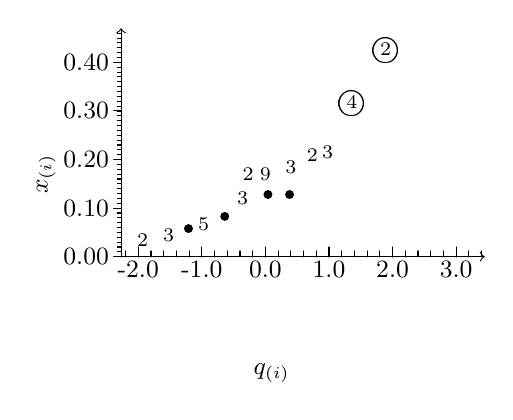
\begin{tikzpicture}[scale=0.95,line join=round,line cap=round]
% 数据坐标 -> cm: x 每单位 0.85cm, y 每单位 6.5cm
\draw[->] (-2.30*0.85,0) -- (3.45*0.85,0);
\draw[->] (-2.27*0.85,0) -- (-2.27*0.85,0.47*6.5);
% x 轴小刻度(每 0.2)与主刻度
\foreach \t in {-2.2,-2.0,...,3.4} {
  \draw (\t*0.85,0) -- (\t*0.85,0.012*6.5);
}
\foreach \t/\lab in {-2/-2.0,-1/-1.0,0/0.0,1/1.0,2/2.0,3/3.0} {
  \draw (\t*0.85,0) -- (\t*0.85,0.020*6.5);
  \node[below,inner sep=1.5pt,font=\small] at (\t*0.85,0) {\lab};
}
% y 轴小刻度(每 0.01)与主刻度
\foreach \t in {0.00,0.01,...,0.46} {
  \draw (-2.27*0.85,\t*6.5) -- (-2.27*0.85-0.05,\t*6.5);
}
\foreach \t/\lab in {0/0.00,0.1/0.10,0.2/0.20,0.3/0.30,0.4/0.40} {
  \draw (-2.27*0.85,\t*6.5) -- (-2.27*0.85-0.10,\t*6.5);
  \node[left,inner sep=1.5pt,font=\small] at (-2.27*0.85-0.10,\t*6.5) {\lab};
}
\node[font=\small,rotate=90] at (-2.27*0.85-1.00,0.17*6.5) {$x_{(i)}$};
\node[font=\small] at (0.1*0.85,-0.24*6.5) {$q_{(i)}$};
% 数据点（同一位置上的点重合为一个点，旁边的整数为点的个数）
\fill (-1.21*0.85,0.058*6.5) circle (1.7pt);
\fill (-0.64*0.85,0.083*6.5) circle (1.7pt);
\fill (0.04*0.85,0.128*6.5) circle (1.7pt);
\fill (0.38*0.85,0.128*6.5) circle (1.7pt);
% 数据点个数标签：\scriptsize + inner sep=1pt，并抬高"2""9"两处避免压点
\node[font=\scriptsize,inner sep=1pt] at (-1.93*0.85,0.033*6.5) {2};
\node[font=\scriptsize,inner sep=1pt] at (-1.52*0.85,0.044*6.5) {3};
\node[font=\scriptsize,inner sep=1pt] at (-0.97*0.85,0.067*6.5) {5};
\node[font=\scriptsize,inner sep=1pt] at (-0.36*0.85,0.120*6.5) {3};
\node[font=\scriptsize,inner sep=1pt] at (-0.27*0.85,0.170*6.5) {2};
\node[font=\scriptsize,inner sep=1pt] at (0.00*0.85,0.170*6.5) {9};
\node[font=\scriptsize,inner sep=1pt] at (0.40*0.85,0.184*6.5) {3};
\node[font=\scriptsize,inner sep=1pt] at (0.74*0.85,0.208*6.5) {2};
\node[font=\scriptsize,inner sep=1pt] at (0.98*0.85,0.214*6.5) {3};
% 离群值
\node[font=\small] at (1.36*0.85,0.310*6.5) {\textcircled{\scriptsize 4}};
\node[font=\small] at (1.89*0.85,0.420*6.5) {\textcircled{\scriptsize 2}};
\end{tikzpicture}
\phantomsection\label{fig:4.6}\mvcap{图 4.6\quad 例 4.10 的辐射量(炉门关闭)数据的 $Q$-$Q$ 图\\
(图中的整数表明在同一位置上的点的个数)}
\end{mvfigure}

对放射量数据, 有些观测值是相等的. 在这情况出现时, 有相同值的那些观测值伴有相同的正态分位数. 这个分位数是用观测值在全都略有不同时所有的分位数的平均值算出的.\hfill$\blacksquare$

Q-Q 图的直线性可以通过计算图中点的相关系数来度量. Q-Q 图的相关系数由下式定义
\phantomsection\label{eq:4-31}
\begin{equation}
r_{Q}=\frac{\sum_{j=1}^{n}(x_{(j)}-\bar{x})(q_{(j)}-\bar{q})}{\sqrt{\sum_{j=1}^{n}(x_{(j)}-\bar{x})^{2}}\sqrt{\sum_{j=1}^{n}(q_{(j)}-\bar{q})^{2}}} \tag{4-31}
\end{equation}
并且可以根据它对正态性进行有力的检验(参见文献[5], [10]和[12]). 形式上, 在显著性水平 $\alpha$ 下, 如果 $r_{Q}$ 降为\hyperref[tab:4.2]{表 4.2} 中适当值之下, 我们拒绝正态性假定.

\begin{mvtable}
\phantomsection\label{tab:4.2}\mvtabcap{表 4.2\quad 对正态性的 $Q$-$Q$ 图相关系数检验的临界点}
\begin{tabular}{cccc}
\toprule
\multirow{2}{*}{样本容量 $n$} & \multicolumn{3}{c}{显著性水平 $\alpha$} \\
\cmidrule(lr){2-4}
 & 0.01 & 0.05 & 0.10 \\
\midrule
5 & 0.829 9 & 0.878 8 & 0.903 2 \\
10 & 0.880 1 & 0.919 8 & 0.935 1 \\
15 & 0.912 6 & 0.938 9 & 0.950 3 \\
20 & 0.926 9 & 0.950 8 & 0.960 4 \\
25 & 0.941 0 & 0.959 1 & 0.966 5 \\
30 & 0.947 9 & 0.965 2 & 0.971 5 \\
35 & 0.953 8 & 0.968 2 & 0.974 0 \\
40 & 0.959 9 & 0.972 6 & 0.977 1 \\
45 & 0.963 2 & 0.974 9 & 0.979 2 \\
\bottomrule
\end{tabular}
\end{mvtable}

%% ===== pg-151 =====

\begin{mvtable}
\centering
{\zihao{6}续表\par}\vspace{2pt}
\begin{tabular}{cccc}
\toprule
\multirow{2}{*}{样本容量 $n$} & \multicolumn{3}{c}{显著性水平 $\alpha$} \\
\cmidrule(lr){2-4}
 & 0.01 & 0.05 & 0.10 \\
\midrule
50 & 0.967 1 & 0.976 8 & 0.980 9 \\
55 & 0.969 5 & 0.978 7 & 0.982 2 \\
60 & 0.972 0 & 0.980 1 & 0.983 6 \\
75 & 0.977 1 & 0.983 8 & 0.986 6 \\
100 & 0.982 2 & 0.987 3 & 0.989 5 \\
150 & 0.987 9 & 0.991 3 & 0.992 8 \\
200 & 0.990 5 & 0.993 1 & 0.994 2 \\
300 & 0.993 5 & 0.995 3 & 0.996 0 \\
\bottomrule
\end{tabular}
\end{mvtable}

\noindent\textbf{例 4.11}\quad \textbf{(正态性的相关系数检验法)}

让我们计算例 4.9(参见\hyperref[fig:4.5]{图 4.5})的 Q-Q 图的相关系数 $r_{Q}$ 并检验正态性.

利用例 4.9 的数据, 我们有 $\bar{x}=0.770$ 以及
\[
\sum_{j=1}^{10}(x_{(j)}-\bar{x})q_{(j)}=8.584,\quad \sum_{j=1}^{10}(x_{(j)}-\bar{x})^{2}=8.472\quad\text{和}\quad \sum_{j=1}^{10}q_{(j)}^{2}=8.795
\]

由于 $\bar{q}=0$
\[
r_{Q}=\frac{8.584}{\sqrt{8.472\times 8.795}}=0.994
\]

在显著性水平 10\% 下, 通过把 $r_{Q}=0.994$ 与\hyperref[tab:4.2]{表 4.2} 中对应于 $n=10$ 和 $\alpha=0.10$ 的表项相对照, 来进行正态性检验. 表项为 0.935 1. 由于 $r_{Q}>0.935\ 1$, 我们不拒绝正态性假定.\hfill$\blacksquare$

与 $r_{Q}$ 不同, 有些软件包评估由夏皮罗(Shapiro)和威尔克(Wilk)(参见文献[12])提出的原始统计量. 它的相关形式对应于用一个标准正态顺序统计量的期望值和它们的协方差的函数来替换 $q_{(j)}$. 我们喜欢 $r_{Q}$, 因为它直接对应于正态的许多散布图中的点. 对于大样本容量, 这两个统计量几乎是相同的(参见文献[13]), 因此, 任何一个都可用来判断拟合的不足.

可以研究多于一个特性的线性组合. 许多统计学家建议标绘
\[
\hat{\mathbf{e}}_{1}'\mathbf{x},\quad \text{其中}\quad \mathbf{S}\hat{\mathbf{e}}_{1}=\hat{\lambda}_{1}\hat{\mathbf{e}}_{1}
\]
式中的 $\hat{\lambda}_{1}$ 是 $\mathbf{S}$ 的最大特征值. 这里 $\mathbf{x}_{(j)}'=[x_{(j1)},x_{(j2)},\cdots,x_{(jp)}]$ 是对 $p$ 个变量 $X_{1},X_{2},\cdots,X_{p}$ 的第 $j$ 个的观测值. 对应于最小特征值的线性组合 $\hat{\mathbf{e}}_{p}'\mathbf{x}_{(j)}$ 也常常被挑选出来进行检验(有关进一步的细节参见第 8 章和文献[6]).

\mvsub{评估二元正态性}

我们会希望检验所有 $2,3,\cdots,p$ 维的分布的正态性假定. 然而, 正如我们已指出的, 对于实际工作, 研究一元和二元分布通常就足够了. 前面我们考虑过一元边缘分布. 现在感兴趣的是检查二元情况.

在第 1 章中, 我们对于表示特征的点对作了散布图. 如果观测值是从一个多元正态分布生成的, 每个二元分布会是正态的, 并且常数密度轮廓线会是椭圆. 散布图显示一个近乎椭圆

%% ===== pg-152 =====

的总形状, 从而与这个结构一致.

此外, 由结论 4.7, 二元结果的集合 $\mathbf{x}$ 满足
\[
(\mathbf{x}-\boldsymbol{\mu})'\boldsymbol{\Sigma}^{-1}(\mathbf{x}-\boldsymbol{\mu})\le \chi_{2}^{2}(0.5)
\]
其概率为 0.5. 因此, 我们应当粗略地期望对于所给椭圆上的样本观测值有相同的百分比(50\%), 该椭圆由下式给出
\[
\{\text{一切满足 } (\mathbf{x}-\bar{\mathbf{x}})'\mathbf{S}^{-1}(\mathbf{x}-\bar{\mathbf{x}})\le \chi_{2}^{2}(0.5) \text{ 的 } \mathbf{x}\}
\]
其中我们用 $\boldsymbol{\mu}$ 的估计值 $\bar{\mathbf{x}}$ 来代替 $\boldsymbol{\mu}$ 并用 $\boldsymbol{\Sigma}^{-1}$ 的估计值 $\mathbf{S}^{-1}$ 来代替 $\boldsymbol{\Sigma}^{-1}$. 否则, 正态性假定就是可疑的.

\noindent\textbf{例 4.12}\quad \textbf{(二元正态性检验)}

虽然不是一个随机样本, 在练习 1.4 中列举了对美国最大的 10 家工业公司的观测值对 $(x_{1}=\text{销售额},x_{2}=\text{利润})$ 组成的数据. 这些数据给出
\[
\bar{\mathbf{x}}=\begin{bmatrix}155.60\\14.70\end{bmatrix},\quad \mathbf{S}=\begin{bmatrix}7\,476.45 & 303.62\\303.62 & 26.19\end{bmatrix}
\]
于是
\[
\mathbf{S}^{-1}=\frac{1}{103\,623.12}\begin{bmatrix}26.19 & -303.62\\-303.62 & 7\,476.45\end{bmatrix}
=\begin{bmatrix}0.000\,253 & -0.002\,930\\-0.002\,930 & 0.072\,148\end{bmatrix}
\]
根据附表 3, $\chi_{2}^{2}(0.5)=1.39$. 因此, 任意满足
\[
\begin{bmatrix}x_{1}-155.60\\x_{2}-14.70\end{bmatrix}'\begin{bmatrix}0.000\,253 & -0.002\,930\\-0.002\,930 & 0.072\,148\end{bmatrix}\begin{bmatrix}x_{1}-155.60\\x_{2}-14.70\end{bmatrix}\le 1.39
\]
的观测值 $\mathbf{x}'=[x_{1},x_{2}]$ 处于估计 50\% 轮廓线的线上或内部, 否则观测值在轮廓线的外部. 在练习 1.4 中第一对观测值是 $[x_{1},x_{2}]'=[108.28,17.05]$. 此时
\[
\begin{bmatrix}108.28-155.60\\17.05-14.70\end{bmatrix}'\begin{bmatrix}0.000\,253 & -0.002\,930\\-0.002\,930 & 0.072\,148\end{bmatrix}\begin{bmatrix}108.28-155.60\\17.05-14.70\end{bmatrix}=1.61>1.39
\]
并且该点落在 50\% 轮廓线之外. 其余 9 个点距 $\bar{\mathbf{x}}$ 的广义距离分别为 0.30, 0.62, 1.79, 1.30, 4.38, 1.64, 3.53, 1.71 和 1.16. 由于这些距离中有 4 个小于 1.39, 数据落在 50\% 轮廓线之内的比例占 0.4. 如果观测值服从正态分布, 我们应期望它们中的大约一半或 5 个处于轮廓线之内. 比例上的差别通常为拒绝二元正态性的看法提供证据; 但是, 本例中的样本容量太小, 仅为 10, 不足以得出这一结论(也参见例 4.13).\hfill$\blacksquare$

计算处于轮廓线内的点的比例, 并将其与理论上的概率进行主观比较, 这是有用的方法, 不过有点粗略. 在判断一个数据集的联合正态性时, 一种更正式的方法是基于广义平方距离
\phantomsection\label{eq:4-32}
\begin{equation}
d_{j}^{2}=(\mathbf{x}_{j}-\bar{\mathbf{x}})'\mathbf{S}^{-1}(\mathbf{x}_{j}-\bar{\mathbf{x}}),\quad j=1,2,\cdots,n \tag{4-32}
\end{equation}
其中 $\mathbf{x}_{1},\mathbf{x}_{2},\cdots,\mathbf{x}_{n}$ 是样本观测值. 我们准备描述的方法不仅仅局限于二元情况, 它对所有 $p\ge 2$ 的情况都适用.

当总体是多元正态的, 且 $n$ 和 $n-p$ 都比 25 或 30 更大时, 平方距离 $d_{1}^{2},d_{2}^{2},\cdots,d_{n}^{2}$ 中的每一个应该表现为一个卡方随机变量[参见结论 4.7 以及\hyperref[eq:4-26]{式(4-26)}和\hyperref[eq:4-27]{式(4-27)}]. 即使这些距离

%% ===== pg-153 =====

不是独立的或不是精确的卡方分布, 把它们当做如此来作图, 也是有用的. 所得到的图称为卡方图或伽马图, 因为卡方分布是更一般的伽马分布的特殊情况(参见文献[6]).

构造卡方图的步骤如下:

\begin{enumerate}[label=\arabic*.,leftmargin=2em,itemsep=2pt]
\item 把\hyperref[eq:4-32]{式(4-32)}中的平方距离从最小到最大排序为 $d_{(1)}^{2}\le d_{(2)}^{2}\le\cdots\le d_{(n)}^{2}$.
\item 画出点对 $\Bigl(q_{c,p}\Bigl(\dfrac{j-\frac{1}{2}}{n}\Bigr),d_{(j)}^{2}\Bigr)$ 的图形, 其中 $q_{c,p}\Bigl(\dfrac{j-\frac{1}{2}}{n}\Bigr)$ 是自由度为 $p$ 的卡方分布的 $100\Bigl(\dfrac{j-\frac{1}{2}}{n}\Bigr)$ 分位数.
\end{enumerate}

分位数是用比例来规定的, 而百分位数是用百分比来规定的.

分位数 $q_{c,p}\Bigl(\dfrac{j-\frac{1}{2}}{n}\Bigr)$ 与卡方分布的上百分位数有关. 具体的, $q_{c,p}\Bigl(\dfrac{j-\frac{1}{2}}{n}\Bigr)=\chi_{p}^{2}\Bigl(\dfrac{n-j+\frac{1}{2}}{n}\Bigr)$.

图形应当类似于一条通过原点且斜率为 1 的直线. 一个系统的弯曲图形表明缺乏正态性. 一个或两个远离直线的点表示大的距离, 或是离群的观测值, 这些都值得进一步注意.

\noindent\textbf{例 4.13}\quad \textbf{(构造卡方图)}

让我们构造在例 4.12 中所给的广义距离的卡方图. 对于 $p=2$ 和 $n=10$ 的有序距离和相应的卡方百分位数列表如下:

\begin{mvtable}
\centering
\mvfit{%
\begin{tabular}{cccccc}
\toprule
$j$ & $d_{(j)}^{2}$ & $q_{c,2}\Bigl(\dfrac{j-\frac{1}{2}}{10}\Bigr)$ & $j$ & $d_{(j)}^{2}$ & $q_{c,2}\Bigl(\dfrac{j-\frac{1}{2}}{10}\Bigr)$ \\
\midrule
1 & 0.30 & 0.10 & 6 & 1.64 & 1.60 \\
2 & 0.62 & 0.33 & 7 & 1.71 & 2.10 \\
3 & 1.16 & 0.58 & 8 & 1.79 & 2.77 \\
4 & 1.30 & 0.86 & 9 & 3.53 & 3.79 \\
5 & 1.61 & 1.20 & 10 & 4.38 & 5.99 \\
\bottomrule
\end{tabular}
}
\end{mvtable}

点对 $\Bigl(q_{c,2}\Bigl(\dfrac{j-\frac{1}{2}}{10}\Bigr),d_{(j)}^{2}\Bigr)$ 的图形示于\hyperref[fig:4.7]{图 4.7}. \hyperref[fig:4.7]{图 4.7} 中的点基本上在一条直线上, 但给定的样本容量小, 我们从该图形的特征很难来拒绝数据的二元正态性. 如果需要对数据作进一步分析, 把它们变换为更接近二元正态的观测值是合理的. 适当的变换方法在 4.8 节中讨论.

除了检验单变量图和散布图外, 我们应通过构造卡方图或 $d^{2}$ 图来检验多元正态性. \hyperref[fig:4.8]{图 4.8} 给出了对计算机生成的含 30 个四元正态随机向量的两个样本所作的 $d^{2}$ 图. 正如所期望的, 该图为直线模式, 但最高的两个或三个有序平方距离的变异性很大.

下面给出一个真实的数据集, 可与生成\hyperref[fig:4.8]{图 4.8} 的模拟数据集进行比较.

\noindent\textbf{例 4.14}\quad \textbf{(评估一个四元数据集的多元正态性)}

\hyperref[tab:4.3]{表 4.3} 中的数据是对 $n=30$ 块木板的每一块的硬度的四种不同的测量 $x_{1},x_{2},x_{3}$ 和 $x_{4}$. 第一个测量需要给木板传送一个向下的冲击波, 第二个测量是当木板振动时测得的, 后两个测量是从静态试验中得到的, 平方距离 $d_{j}^{2}=(\mathbf{x}_{j}-\bar{\mathbf{x}})'\mathbf{S}^{-1}(\mathbf{x}_{j}-\bar{\mathbf{x}})$ 也在表中给出.

%% ===== pg-154 =====

\begin{mvfigure}
\centering
\begin{tikzpicture}[scale=0.62]
\draw[->] (0,0)--(7.8,0) node[right,font=\small]{$q_{c,2}\Bigl(\dfrac{j-\frac{1}{2}}{10}\Bigr)$};
\draw[->] (0,0)--(0,5.5) node[above,font=\small]{$d_{(j)}^{2}$};
\foreach \x in {1,2,3,4,5,6,7} \draw (\x,0.08)--(\x,-0.08) node[below,font=\scriptsize]{\x};
\foreach \y in {0.5,1,1.5,2,2.5,3,3.5,4,4.5,5} \draw (0.08,\y)--(-0.08,\y) node[left,font=\scriptsize]{\y};
\foreach \p in {(0.10,0.30),(0.33,0.62),(0.58,1.16),(0.86,1.30),(1.20,1.61),(1.60,1.64),(2.10,1.71),(2.77,1.79),(3.79,3.53),(5.99,4.38)} \fill \p circle (2pt);
\end{tikzpicture}
\phantomsection\label{fig:4.7}\mvcap{图 4.7\quad 例 4.13 中有序距离的卡方图}
\end{mvfigure}

\begin{mvfigure}
\centering
\begin{tikzpicture}[scale=0.5]
\draw[->] (0,0)--(13,0) node[right,font=\small]{$q_{c,4}\Bigl(\dfrac{j-\frac{1}{2}}{30}\Bigr)$};
\draw[->] (0,0)--(0,10.5) node[above,font=\small]{$d_{(j)}^{2}$};
\foreach \x in {2,4,6,8,10,12} \draw (\x,0.1)--(\x,-0.1) node[below,font=\scriptsize]{\x};
\foreach \y in {2,4,6,8,10} \draw (0.1,\y)--(-0.1,\y) node[left,font=\scriptsize]{\y};
\foreach \p in {(0.3,0.2),(0.6,0.5),(0.9,0.7),(1.2,0.9),(1.5,1.1),(1.8,1.4),(2.1,1.7),(2.4,2.0),(2.7,2.3),(3.0,2.6),(3.3,2.9),(3.6,3.2),(3.9,3.5),(4.2,3.8),(4.5,4.1),(4.8,4.4),(5.1,4.7),(5.4,5.0),(5.7,5.2),(6.0,5.4),(6.3,5.6),(6.6,5.9),(6.9,6.1),(7.2,6.3),(7.5,6.5),(7.8,6.7),(8.1,6.9),(8.4,7.1),(9.6,7.5),(11.2,9.2)} \fill \p circle (1.7pt);
\end{tikzpicture}
\hspace{1.2cm}
\begin{tikzpicture}[scale=0.5]
\draw[->] (0,0)--(13,0) node[right,font=\small]{$q_{c,4}\Bigl(\dfrac{j-\frac{1}{2}}{30}\Bigr)$};
\draw[->] (0,0)--(0,10.5) node[above,font=\small]{$d_{(j)}^{2}$};
\foreach \x in {2,4,6,8,10,12} \draw (\x,0.1)--(\x,-0.1) node[below,font=\scriptsize]{\x};
\foreach \y in {2,4,6,8,10} \draw (0.1,\y)--(-0.1,\y) node[left,font=\scriptsize]{\y};
\foreach \p in {(0.4,0.2),(0.7,0.4),(1.0,0.6),(1.3,0.9),(1.6,1.2),(1.9,1.5),(2.2,1.8),(2.5,2.1),(2.8,2.4),(3.1,2.7),(3.4,3.0),(3.7,3.3),(4.0,3.6),(4.3,3.9),(4.6,4.2),(4.9,4.5),(5.2,4.8),(5.5,5.0),(5.8,5.2),(6.1,5.4),(6.4,5.6),(6.7,5.8),(7.0,6.0),(7.3,6.2),(7.6,6.4),(7.9,6.6),(8.2,6.8),(8.5,7.0),(9.8,7.4),(11.6,8.6)} \fill \p circle (1.7pt);
\end{tikzpicture}
\phantomsection\label{fig:4.8}\mvcap{图 4.8\quad 两个 $n=30$ 的模拟四元正态数据集的卡方图}
\end{mvfigure}

\begin{mvtable}
\centering
\phantomsection\label{tab:4.3}\mvtabcap{表 4.3\quad 硬度的四种测量值}
\mvfit{%
\begin{tabular}{cccccc@{\qquad}cccccc}
\toprule
\makecell{观测值\\序号} & $x_{1}$ & $x_{2}$ & $x_{3}$ & $x_{4}$ & $d^{2}$ & \makecell{观测值\\序号} & $x_{1}$ & $x_{2}$ & $x_{3}$ & $x_{4}$ & $d^{2}$ \\
\midrule
1 & 1\,889 & 1\,651 & 1\,561 & 1\,778 & 0.60 & 16 & 1\,954 & 2\,149 & 1\,180 & 1\,281 & 16.85 \\
2 & 2\,403 & 2\,048 & 2\,087 & 2\,197 & 5.48 & 17 & 1\,325 & 1\,170 & 1\,002 & 1\,176 & 3.50 \\
3 & 2\,119 & 1\,700 & 1\,815 & 2\,222 & 7.62 & 18 & 1\,419 & 1\,371 & 1\,252 & 1\,308 & 3.99 \\
4 & 1\,645 & 1\,627 & 1\,110 & 1\,533 & 5.21 & 19 & 1\,828 & 1\,634 & 1\,602 & 1\,755 & 1.36 \\
5 & 1\,976 & 1\,916 & 1\,614 & 1\,883 & 1.40 & 20 & 1\,725 & 1\,594 & 1\,313 & 1\,646 & 1.46 \\
6 & 1\,712 & 1\,712 & 1\,439 & 1\,546 & 2.22 & 21 & 2\,276 & 2\,189 & 1\,547 & 2\,111 & 9.90 \\
7 & 1\,943 & 1\,685 & 1\,271 & 1\,671 & 4.99 & 22 & 1\,899 & 1\,614 & 1\,422 & 1\,477 & 5.06 \\
8 & 2\,104 & 1\,820 & 1\,717 & 1\,874 & 1.49 & 23 & 1\,633 & 1\,513 & 1\,290 & 1\,516 & 0.80 \\
9 & 2\,983 & 2\,794 & 2\,412 & 2\,581 & 12.26 & 24 & 2\,061 & 1\,867 & 1\,646 & 2\,037 & 2.54 \\
10 & 1\,745 & 1\,600 & 1\,384 & 1\,508 & 0.77 & 25 & 1\,856 & 1\,493 & 1\,356 & 1\,533 & 4.58 \\
11 & 1\,710 & 1\,591 & 1\,518 & 1\,667 & 1.93 & 26 & 1\,727 & 1\,412 & 1\,238 & 1\,469 & 3.40 \\
12 & 2\,046 & 1\,907 & 1\,627 & 1\,898 & 0.46 & 27 & 2\,168 & 1\,896 & 1\,701 & 1\,834 & 2.38 \\
13 & 1\,840 & 1\,841 & 1\,595 & 1\,741 & 2.70 & 28 & 1\,655 & 1\,675 & 1\,414 & 1\,597 & 3.00 \\
14 & 1\,867 & 1\,685 & 1\,493 & 1\,678 & 0.13 & 29 & 2\,326 & 2\,301 & 2\,065 & 2\,234 & 6.28 \\
15 & 1\,859 & 1\,649 & 1\,389 & 1\,714 & 1.08 & 30 & 1\,490 & 1\,382 & 1\,214 & 1\,284 & 2.58 \\
\bottomrule
\end{tabular}
}
\end{mvtable}

\noindent{\zihao{6}资料来源: 数据经 William Galligan 许可使用.}

%% ===== pg-155 =====

边缘分布很像是正态的, 只有样本 (木板)9 有可能例外 (参见练习 4.33).

为了进一步评价多元正态性, 我们作卡方图, 如\hyperref[fig:4.9]{图 4.9} 所示. 具有最大平方距离的两个样本很清楚偏离了直线图形. 这两个点以及平方距离其次大的一个两点, 使得图形在上面的末端弯曲. 在例 4.15 中我们将回过来再对这一图形进行讨论.

\begin{mvfigure}
\centering
\begin{tikzpicture}[scale=0.62]
\draw[->] (0,0)--(13.2,0) node[right,font=\small]{$q_{c,2}\Bigl(\dfrac{j-\frac{1}{2}}{30}\Bigr)$};
\draw[->] (0,0)--(0,17) node[above,font=\small]{$d_{(j)}^{2}$};
\foreach \x in {2,4,6,8,10,12} \draw (\x,0.15)--(\x,-0.15) node[below,font=\scriptsize]{\x};
\foreach \y in {2,4,6,8,10,12,14,16} \draw (0.15,\y)--(-0.15,\y) node[left,font=\scriptsize]{\y};
% 参考直线 y = x
\draw[dashed] (0,0)--(11,11);
% 数据点（近似 q-q 图）
\foreach \p in {(0.3,0.3),(0.7,0.7),(1.0,0.9),(1.4,1.5),(1.8,1.7),(2.2,2.2),(2.6,2.5),(3.0,3.0),(3.4,3.3),(3.8,3.9),(4.2,4.1),(4.6,4.5),(5.0,5.0),(5.4,5.3),(5.8,5.9),(6.2,6.1),(6.6,6.5),(7.0,7.0),(7.4,7.6),(7.8,8.0),(8.2,8.6),(8.6,9.2),(9.0,9.8),(9.4,10.4),(9.8,11.2)} \fill \p circle (2.2pt);
% 末端偏离点
\fill (10.2,12.0) circle (2.2pt);
\fill (10.6,12.8) circle (2.2pt);
\draw (10.6,12.8) circle (5pt);
\fill (11.0,16.0) circle (2.2pt);
\end{tikzpicture}
\phantomsection\label{fig:4.9}\mvcap{图 4.9\quad 例 4.14 中数据的卡方图}
\end{mvfigure}

我们已经讨论了一些检验正态性假定的简单方法. 特别地, 我们提倡计算 $d_{j}^{2},j=1,2,\cdots,n$ [参见\hyperref[eq:4-32]{式(4-32)}], 并将结果与 $\chi^{2}$ 分位数相比较. 例如, 如果:

1.\quad 大约有一半的 $d_{j}^{2}$ 小于或等于 $q_{c,2}(0.50)$.

2.\quad 分别与 $q_{c,2}\Bigl(\dfrac{1-\frac{1}{2}}{n}\Bigr),q_{c,2}\Bigl(\dfrac{2-\frac{1}{2}}{n}\Bigr),\cdots,q_{c,2}\Bigl(\dfrac{n-\frac{1}{2}}{n}\Bigr)$ 相对应的顺序.

平方距离 $d_{(1)}^{2}\le d_{(2)}^{2}\le\cdots\le d_{(n)}^{2}$ 的图形近似是一条通过原点且斜率为 1 的直线. 那么, 就表明是 $p$ 元正态的 (关于确定正态性方法的更完整的说明参见文献 [6]).

我们在本节结束时, 要注意一切拟合优度的度量方法具有同样严重的缺点. 当样本容量很小, 只有最异常的情况会确定为缺乏拟合. 另一方面, 样本很大时, 总量产生统计上显著的缺乏拟合. 然而, 对规定的分布的偏离可能很小, 这对推断结论在技术上并不重要.

\section{搜寻离群值及“清洁”数据}
\phantomsection\label{sec:4.7}

大多数数据集含有一个或几个异常的观测结果, 它们似乎不属于这个由其他观测值产生的变异性的模型. 在一个单一特性的数据中, 异常观测值相对于其他值来说, 或者是很大或者是很小. 在多元数据下情况可能会更为复杂. 在着手鉴别离群值的问题之前, 必须强调不是所有的离群值都是错误的数据. 它们有可能是一聚类的一部分, 并可以使我们更好地理解所研究的现象.

只要可能, 最好是直观地搜寻出离群值. 当观测值的个数 $n$ 很大时, 点图是不可行的. 当特性 $p$ 的数目很大时, 散布图的数目 $p(p-1)/2$ 很大, 会阻止对它们进行总的观察. 即使如此, 我们建议只要有可能, 应当首先直观地观察数据.

我们应当观察什么? 对于一个单一的随机变量, 问题是一维的, 我们寻找远离其他点的观测值. 例如, 点图

%% ===== pg-156 =====

\begin{center}
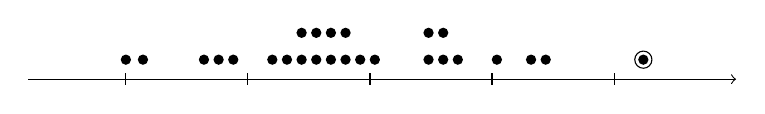
\begin{tikzpicture}[scale=0.62]
\draw[->] (0,0)--(14.5,0);
\foreach \x in {2,4.5,7,9.5,12} \draw (\x,0.12)--(\x,-0.12);
\foreach \x in {2.0,2.35,3.6,3.9,4.2,5.0,5.3,5.6,5.9,6.2,6.5,6.8,7.1,8.2,8.5,8.8,9.6,10.3,10.6} \fill (\x,0.4) circle (3pt);
\foreach \x in {5.6,5.9,6.2,6.5,8.2,8.5} \fill (\x,0.95) circle (3pt);
\draw (12.6,0.4) circle (5pt);
\fill (12.6,0.4) circle (3pt);
\end{tikzpicture}
\end{center}

中显示了唯一的一个大观测值(带圈的点).

在二维情形中, 情况较为复杂. \hyperref[fig:4.10]{图 4.10} 显示了有两个异常观测值的情况.

\begin{mvfigure}
\centering
\begin{tikzpicture}[scale=0.72]
\draw[->] (0,0)--(8.8,0) node[right,font=\small]{$x_{1}$};
\draw[->] (0,0)--(0,9.6) node[above,font=\small]{$x_{2}$};
% x2 的垂直边缘点图
\foreach \y in {0.5,0.8,1.1,1.35,1.5,1.65,1.8,2.0,2.15,2.3,2.45,2.6,2.75,2.9,3.05,3.2,3.35,3.5,3.65,3.8,3.95,4.1,4.3,4.5,4.7,4.9,5.1,5.3,5.5,5.7,5.9,6.1,6.3,6.5} \fill (1.0,\y) circle (2.2pt);
% 散布点云
\foreach \p in {(2.6,1.4),(3.0,1.6),(3.3,1.3),(3.6,2.0),(3.9,2.4),(4.2,2.2),(4.4,2.7),(4.6,3.0),(4.8,3.3),(5.0,2.9),(5.2,3.5),(5.4,3.8),(5.6,3.6),(5.8,4.1),(6.0,4.3),(6.2,4.0),(6.4,4.5),(6.6,4.2),(6.8,4.7),(7.0,5.0),(7.2,4.6),(7.4,5.2),(7.6,5.4),(6.3,5.0),(6.5,5.4),(5.9,4.8),(5.6,4.6),(5.2,4.4),(4.8,3.9),(4.4,3.4)} \fill \p circle (2.2pt);
% 带圈的离群值
\draw (1.0,8.4) circle (5pt); \fill (1.0,8.4) circle (2.2pt);
\draw (6.2,7.5) circle (5pt); \fill (6.2,7.5) circle (2.2pt);
\draw (6.6,2.0) circle (5pt); \fill (6.6,2.0) circle (2.2pt);
% x1 的底部边缘点图
\foreach \x in {0.6,0.9,1.2,1.5,1.8,2.1,2.4,2.7,3.0,3.3,3.6,3.9,4.2,4.5,4.8,5.1,5.4,5.7,6.0,6.3,7.0,7.3} \fill (\x,-0.8) circle (2.2pt);
\draw (6.6,-0.8) circle (5pt); \fill (6.6,-0.8) circle (2.2pt);
\end{tikzpicture}
\phantomsection\label{fig:4.10}\mvcap{图 4.10\quad 两个离群值: 一个单变量和一个双变量}
\end{mvfigure}

该图右上角带圈的数据点远离图中的图形, 并且它的第二个坐标较其余的 $x_{2}$ 的测量值大, 正如垂直点图所显示的. 也用圆圈圈起的第二个离群值远离其余点的椭圆形状, 但分别来看, 它的每一个分量都有一个正常的值. 这个离群值不可能靠观察边缘点图搜寻出来.

在高维中, 可能有的离群值不能从单变量散布图或者甚至二维散布图中搜寻出来. 在这里, $(\mathbf{x}_{j}-\bar{\mathbf{x}})'\mathbf{S}^{-1}(\mathbf{x}_{j}-\bar{\mathbf{x}})$ 的大值表明有异常观测值, 即使它不能直观地看到.

\mvsub{搜寻离群值的步骤}

\begin{enumerate}[label=\arabic*.,leftmargin=2em,itemsep=2pt]
\item 对于每个变量作一个点图.
\item 对于每对变量作一个散布图.
\item 对于 $j=1,2,\cdots,n$ 和每列 $k=1,2,\cdots,p$, 计算标准化值 $z_{jk}=(x_{jk}-\bar{x}_{k})/\sqrt{s_{kk}}$, 检查这些标准化值中的大值和小值.
\item 计算广义平方距离 $(\mathbf{x}_{j}-\bar{\mathbf{x}})'\mathbf{S}^{-1}(\mathbf{x}_{j}-\bar{\mathbf{x}})$, 对异常大的值检查这些距离. 在卡方图中, 这些点应当是离原点最远的点.
\end{enumerate}

步骤 3 中, “大”应当理解为与样本容量和变量个数相比较而言. 有 $n\times p$ 个标准化值. 当 $n=100$ 且 $p=5$ 时, 有 500 个值. 即使数据来自一个恰好正态的多元分布, 可预期这些值中的 1 或 2 个大于 3 或小于 $-3$. 对于一个中等的样本容量, 作为一个指标, 3.5 可以认为是大的.

在步骤 4 中, “大”是由自由度为 $p$ 的卡方分布的一个恰当的百分位数来度量的. 如果样

%% ===== pg-157 =====

本容量是 $n=100$, 我们应当预期有 5 个观测值的 $d_{j}^{2}$ 值超过卡方分布的上第 5 个百分位数. 一个较为极端的百分位数应用于确定不拟合其余数据的图形的观测值.

\hyperref[tab:4.3]{表 4.3} 中给出的关于木板的数据已经进行过一些清理. 来自同一研究的类似数据集还包含对 $x_{5}=$张力强度的数据. 下表的各行列出的是从 112 个观测值向量中选出的 9 个向量, 并给出了其标准化值.

\begin{mvtable}
\centering
\begin{tabular}{ccccc|ccccc}
\toprule
$x_{1}$ & $x_{2}$ & $x_{3}$ & $x_{4}$ & $x_{5}$ & $z_{1}$ & $z_{2}$ & $z_{3}$ & $z_{4}$ & $z_{5}$ \\
\midrule
$\vdots$ & $\vdots$ & $\vdots$ & $\vdots$ & $\vdots$ & $\vdots$ & $\vdots$ & $\vdots$ & $\vdots$ & $\vdots$ \\
1\,631 & 1\,528 & 1\,452 & 1\,559 & 1\,602 & 0.06 & -0.15 & 0.05 & 0.28 & -0.12 \\
1\,770 & 1\,677 & 1\,707 & 1\,738 & 1\,785 & 0.64 & 0.43 & 1.07 & 0.94 & 0.60 \\
1\,376 & 1\,190 & 723 & 1\,285 & 2\,791 & -1.01 & -1.47 & -2.87 & -0.73 & \tikz[baseline=(a.base)]\node[draw,circle,inner sep=1pt](a){4.57}; \\
1\,705 & 1\,577 & 1\,332 & 1\,703 & 1\,664 & 0.37 & 0.04 & -0.43 & 0.81 & 0.13 \\
1\,643 & 1\,535 & 1\,510 & 1\,494 & 1\,582 & 0.11 & -0.12 & 0.28 & 0.04 & -0.20 \\
1\,567 & 1\,510 & 1\,301 & 1\,405 & 1\,553 & -0.21 & -0.22 & -0.56 & -0.28 & -0.31 \\
1\,528 & 1\,591 & 1\,714 & 1\,685 & 1\,698 & -0.38 & 0.10 & 1.10 & 0.75 & 0.26 \\
1\,803 & 1\,826 & 1\,748 & 2\,746 & 1\,764 & 0.78 & 1.01 & 1.23 & \tikz[baseline=(b.base)]\node[draw,circle,inner sep=1pt](b){4.65}; & 0.52 \\
1\,587 & 1\,554 & 1\,352 & 1\,554 & 1\,551 & -0.13 & -0.05 & -0.35 & 0.26 & -0.32 \\
$\vdots$ & $\vdots$ & $\vdots$ & $\vdots$ & $\vdots$ & $\vdots$ & $\vdots$ & $\vdots$ & $\vdots$ & $\vdots$ \\
\bottomrule
\end{tabular}
\end{mvtable}

标准化值是根据从所有 112 个观测值计算出的样本均值和方差得到的. 表中有两个极端标准化值. 这两个值都太大, 超过 4.5. 在研究时, 研究人员是在记录本中用手记录测量值, 然后进行计算, 得出表中的值. 当他们根据分析结果核对这两个值的记录时, 发现了错误所在. 值 $x_{5}=2791$ 被改为 1241, $x_{4}=2746$ 被改为 1670. 通过找到标准化值的大约首位数字的位置, 就可以迅速地发现在个别变量上的错误读数.

下面的例题返回到例 4.14 中讨论过的木板数据.

\noindent\textbf{例 4.15}\quad \textbf{(在木板数据中搜寻离群值)}

\hyperref[tab:4.4]{表 4.4} 包含了\hyperref[tab:4.3]{表 4.3} 的数据以及标准化观测值. 这些数据由硬度的四种不同的测量值 $x_{1},x_{2},x_{3}$ 和 $x_{4}$ 组成, 每种都有 $n=30$ 块木板. 第一个测量值是向下传送一个冲击波给木板, 第二个测量值是当木板振动时确定的, 最后两个测量值是从静态的试验得到的. 标准化的测量值是
\[
z_{jk}=\frac{x_{jk}-\bar{x}_{k}}{\sqrt{s_{kk}}},\quad k=1,2,3,4;\quad j=1,2,\cdots,30
\]
距离的平方是 $d_{j}^{2}=(\mathbf{x}_{j}-\bar{\mathbf{x}})'\mathbf{S}^{-1}(\mathbf{x}_{j}-\bar{\mathbf{x}})$.

\hyperref[tab:4.4]{表 4.4} 中最后一栏显示出样本 16 是一个多元离群值, 因为 $\chi_{4}^{2}(0.005)=14.86$; 所有的单个测量值都处于它们各自的单变量散布范围之内. 样本 9 也有一个大的 $d^{2}$ 值.

这两个平方距离较大的样本(9 和 16), 十分明显与\hyperref[fig:4.9]{图 4.9} 中的其余部分不同. 一旦这两点被除去, 剩余部分的图形符合期望的直线关系. 对于木板硬度测量的散布图, 在\hyperref[fig:4.11]{图 4.11} 中给出. 图中的实心圆点对应于样本 9 和 16. 虽然样本 16 的点在所有图中都与众不同, 样本 9 的点在 $x_{3}$ 与 $x_{1}$ 的散布图中是“隐藏”的, 并且在 $x_{1}$ 与 $x_{2}$ 的散布图中几乎是隐藏的. 然而, 当所有四个变量都考虑时, 样本 9 很清楚地确定为一个多元离群值.

%% ===== pg-158 =====

\begin{mvtable}
\centering
\phantomsection\label{tab:4.4}\mvtabcap{表 4.4\quad 硬度的四种测量值及标准化值}
\begin{longtable}{cccc@{\qquad}c@{\qquad}ccccc}\toprule
$x_{1}$ & $x_{2}$ & $x_{3}$ & $x_{4}$ & \makecell{观测值\\序号} & $z_{1}$ & $z_{2}$ & $z_{3}$ & $z_{4}$ & $d^{2}$ \\
\midrule
\endfirsthead
\multicolumn{10}{c}{\zihao{6}续表}\\
\toprule
$x_{1}$ & $x_{2}$ & $x_{3}$ & $x_{4}$ & \makecell{观测值\\序号} & $z_{1}$ & $z_{2}$ & $z_{3}$ & $z_{4}$ & $d^{2}$ \\
\midrule
\endhead
\bottomrule
\endlastfoot

1\,889 & 1\,651 & 1\,561 & 1\,778 & 1 & -0.1 & -0.3 & 0.2 & 0.2 & 0.60 \\
2\,403 & 2\,048 & 2\,087 & 2\,197 & 2 & 1.5 & 0.9 & 1.9 & 1.5 & 5.48 \\
2\,119 & 1\,700 & 1\,815 & 2\,222 & 3 & 0.7 & -0.2 & 1.0 & 1.5 & 7.62 \\
1\,645 & 1\,627 & 1\,110 & 1\,533 & 4 & -0.8 & -0.4 & -1.3 & -0.6 & 5.21 \\
1\,976 & 1\,916 & 1\,614 & 1\,883 & 5 & 0.2 & 0.5 & 0.3 & 0.5 & 1.40 \\
1\,712 & 1\,712 & 1\,439 & 1\,546 & 6 & -0.6 & -0.1 & -0.2 & -0.6 & 2.22 \\
1\,943 & 1\,685 & 1\,271 & 1\,671 & 7 & 0.1 & -0.2 & -0.8 & -0.2 & 4.99 \\
2\,104 & 1\,820 & 1\,717 & 1\,874 & 8 & 0.6 & 0.2 & 0.7 & 0.5 & 1.49 \\
2\,983 & 2\,794 & 2\,412 & 2\,581 & 9 & 3.3 & 3.3 & 3.0 & 2.7 & \tikz[baseline=(a.base)]\node[draw,circle,inner sep=1pt](a){12.26}; \\
1\,745 & 1\,600 & 1\,384 & 1\,508 & 10 & -0.5 & -0.5 & -0.4 & -0.7 & 0.77 \\
1\,710 & 1\,591 & 1\,518 & 1\,667 & 11 & -0.6 & -0.5 & 0.0 & -0.2 & 1.93 \\
2\,046 & 1\,907 & 1\,627 & 1\,898 & 12 & 0.4 & 0.5 & 0.4 & 0.5 & 0.46 \\
1\,840 & 1\,841 & 1\,595 & 1\,741 & 13 & -0.2 & 0.3 & 0.3 & 0.0 & 2.70 \\
1\,867 & 1\,685 & 1\,493 & 1\,678 & 14 & -0.1 & -0.2 & -0.1 & -0.1 & 0.13 \\
1\,859 & 1\,649 & 1\,389 & 1\,714 & 15 & -0.1 & -0.3 & -0.4 & -0.0 & 1.08 \\
1\,954 & 2\,149 & 1\,180 & 1\,281 & 16 & 0.1 & 1.3 & -1.1 & -1.4 & \tikz[baseline=(b.base)]\node[draw,circle,inner sep=1pt](b){16.85}; \\
1\,325 & 1\,170 & 1\,002 & 1\,176 & 17 & -1.8 & -1.8 & -1.7 & -1.7 & 3.50 \\
1\,419 & 1\,371 & 1\,252 & 1\,308 & 18 & -1.5 & -1.2 & -0.8 & -1.3 & 3.99 \\
1\,828 & 1\,634 & 1\,602 & 1\,755 & 19 & -0.2 & -0.4 & 0.3 & 0.1 & 1.36 \\
1\,725 & 1\,594 & 1\,313 & 1\,646 & 20 & -0.6 & -0.5 & -0.6 & -0.2 & 1.46 \\
2\,276 & 2\,189 & 1\,547 & 2\,111 & 21 & 1.1 & 1.4 & 0.1 & 1.2 & 9.90 \\
1\,899 & 1\,614 & 1\,422 & 1\,477 & 22 & -0.0 & -0.4 & -0.3 & -0.8 & 5.06 \\
1\,633 & 1\,513 & 1\,290 & 1\,516 & 23 & -0.8 & -0.7 & -0.7 & -0.6 & 0.80 \\
2\,061 & 1\,867 & 1\,646 & 2\,037 & 24 & 0.5 & 0.4 & 0.5 & 1.0 & 2.54 \\
1\,856 & 1\,493 & 1\,356 & 1\,533 & 25 & -0.2 & -0.8 & -0.5 & -0.6 & 4.58 \\
1\,727 & 1\,412 & 1\,238 & 1\,469 & 26 & -0.6 & -1.1 & -0.9 & -0.8 & 3.40 \\
2\,168 & 1\,896 & 1\,701 & 1\,834 & 27 & 0.8 & 0.5 & 0.6 & 0.3 & 2.38 \\
1\,655 & 1\,675 & 1\,414 & 1\,597 & 28 & -0.8 & -0.2 & -0.3 & -0.4 & 3.00 \\
2\,326 & 2\,301 & 2\,065 & 2\,234 & 29 & 1.3 & 1.7 & 1.8 & 1.6 & 6.28 \\
1\,490 & 1\,382 & 1\,214 & 1\,284 & 30 & -1.3 & -1.2 & -1.0 & -1.4 & 2.58 \\
\end{longtable}
\end{mvtable}

专门研究木材性质的科学家们, 推测样本 9 是异乎寻常的没有疤痕, 所以十分坚硬. 样本 16 也显得有点异常, 因为它的两个动态的测量值超过平均数而两个静态的测量值都低于平均数. 可惜, 对于这个样本进一步的研究已不可能, 因为无法再获得资料了.

%% ===== pg-159 =====

% ---- pg-159 （书页 147） ----

\begin{mvfigure}
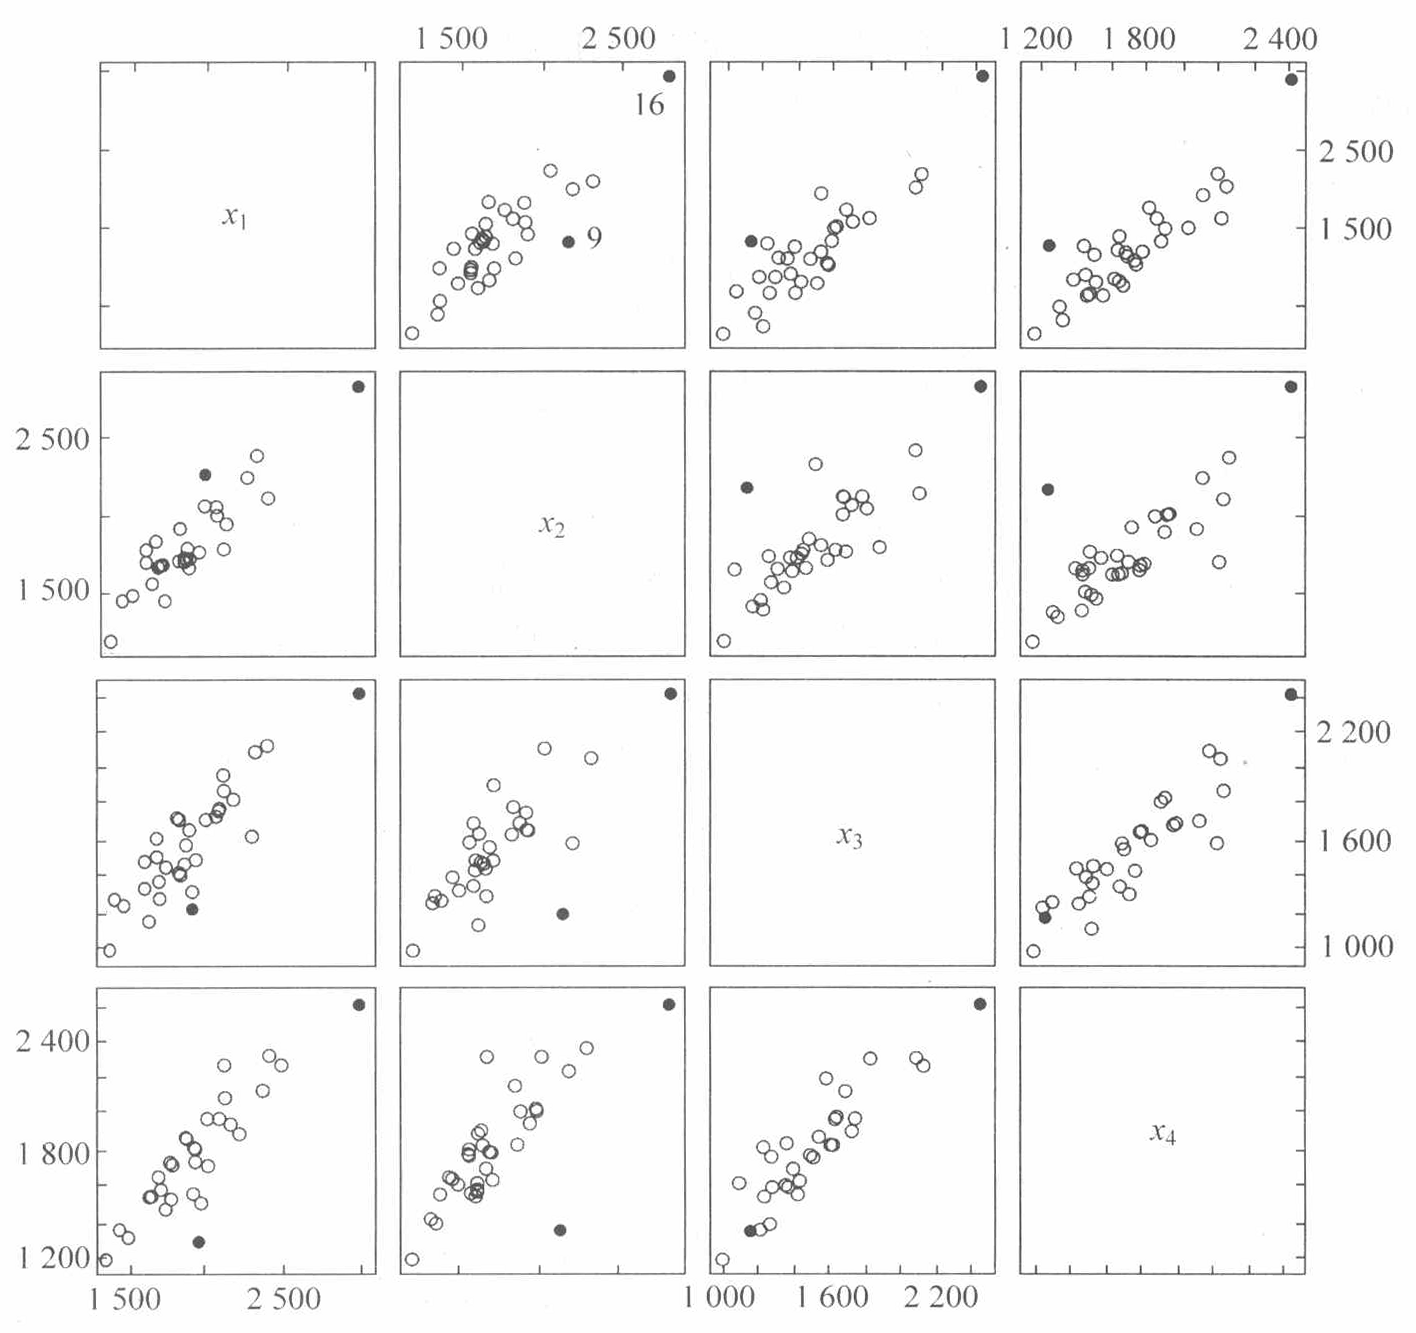
\includegraphics[width=119.9mm]{figs/fig_pg159_1.png}
\phantomsection\label{fig:4.11}\mvcap{图 4.11\quad 木板硬度数据的散布图,其中样本 9 和 16 用实圆点代表}
\end{mvfigure}
\hfill$\blacksquare$

如果离群值被确定, 应当对其内容细查, 正如例 4.15 中在木板硬度数据的例子中所做的. 视离群值的特性和研究的目的而定, 在以后的分析中, 离群值可以删去或适当地“加权”.

虽然许多统计方法假定正态总体, 那些基于样本均值向量的方法通常不会受几个中等的离群值干扰. 霍金斯(Hawkins)(参见文献[7])给出了关于离群值问题的广泛论述.

\section{变换到接近正态性}  % 原书 4.8
\phantomsection\label{sec:4.8}

如果正态性不是一个可行的假定, 下一步该怎么办? 一个选择是不管正态性检验的结论, 把数据当做正态分布来继续进行. 我们不推荐这种做法. 因为在许多情况下, 它可能会导致错误的结论. 第二个选择是通过考虑数据变换, 使非正态数据更加“朝向正态”. 在适当数据变换后, 就可以实现正态理论分析.

变换无非是用不同的单位对数据进行重新表述. 例如, 正观测值的直方图显示出长的右尾时, 通过取对数或平方根来变换观测值, 经常显著地改进其关于均值的对称性, 并且提高对正态分布的近似程度. 新单位对所研究的特性常常提供更自然的表达式.

按照(1)理论上的考虑或(2)数据本身(或两者)提出适当的变换. 理论上已经证明对属于计数的数据取平方根通常可使之更接近正态. 类似地, 对数变换适用于比例, 而将费希尔(Fisher)的 $z$ 变换应用于相关系数, 可产生近似正态分布的量.

%% ===== pg-160 =====

% ---- pg-160 （书页 148） ----

\begin{mvframe}[向正态性接近的有用变换]
\begin{tabular}{llr}
原来的标度 & 变换后的标度 & \\
1. 计数, $y$ & $\sqrt{y}$ & \\
2. 比例, $\hat{p}$ & $\mathrm{logit}(\hat{p}) = \dfrac{1}{2}\log\left(\dfrac{\hat{p}}{1-\hat{p}}\right)$ & (4-33)\\
3. 相关系数, $r$ & 费希尔 $z(r) = \dfrac{1}{2}\log\left(\dfrac{1+r}{1-r}\right)$ & \\
\end{tabular}
\end{mvframe}

在许多情况中, 选择何种变换来改进对正态性的近似, 不是很明显. 对于这种情况, 令数据假设一个变换是方便的. 为此目的一个有效的变换类是幂变换.

幂变换只对正变量定义. 然而, 这并不像看起来的那样有局限性, 因为如果某些值是负的, 可以把数据集中的每个观测值加上一个常数.

设 $x$ 表示一个任意的观测值. 幂变换是用参数 $\lambda$ 来标记. 对于 $\lambda$ 来说, 一个给定值意味着一个具体的变换. 例如, 对 $x$ 采用 $\lambda = -1$, 由于 $x^{-1} = 1/x$, $\lambda$ 的这个选择相当于倒数变换. 我们可以按照 $x$ 的幂 $\lambda$ 的范围从负到正来描绘变换的类. 对于 $\lambda = 0$, 我们定义 $x^0 = \ln x$. 可能变换的系列为
\[
\underbrace{\cdots, x^{-1} = \frac{1}{x}, x^0 = \ln x, x^{1/4} = \sqrt[4]{x}, x^{1/2} = \sqrt{x}}_{x\text{ 的大值缩小}}, \qquad \underbrace{x^2, x^3, \cdots}_{x\text{ 的大值增加}}
\]

为了选择一个幂变换, 研究者察看边缘点图或直方图, 并判断是否有大值要“向里拉”或“向外推”以改进关于均值的对称性. 用上述的几个变换反复计算, 以达到改进的目的. 最后的选择总是应当通过 Q-Q 图或其他方法进行检查, 以弄清尝试性的正态假定是否令人满意.

我们已讨论过的变换是基于数据进行的, 即只有数据形态本身影响对适当变换方法的选择. 我们没有考虑外部因素, 虽然实际使用何种变换方法, 要由数据和数据之外的因素(例如解释的简单性或容易性)所反映的综合信息来确定.

有一种方便的分析方法可用于选择幂变换. 我们首先把注意力集中在一元情况.

博克斯(Box)和考克斯(Cox)考虑有稍微修改的幂类变换(参见文献[3])
\phantomsection\label{eq:4-34}
\begin{equation}
x^{(\lambda)} = \begin{cases} \dfrac{x^\lambda - 1}{\lambda} & \lambda \neq 0 \\[2ex] \ln x & \lambda = 0 \end{cases} \tag{4-34}
\end{equation}
它在 $x>0$ 时对 $\lambda$ 是连续的(参见文献[8]). 给定观测值 $x_1, x_2, \cdots, x_n$, 选择适当的幂 $\lambda$ 的博克斯-考克斯解就是使式
\phantomsection\label{eq:4-35}
\begin{equation}
l(\lambda) = -\frac{n}{2}\ln\left[\frac{1}{n}\sum_{j=1}^{n}\left(x_j^{(\lambda)} - \overline{x^{(\lambda)}}\right)^2\right] + (\lambda - 1)\sum_{j=1}^{n}\ln x_j \tag{4-35}
\end{equation}
最大化的解.

注意到 $x_j^{(\lambda)}$ 是由\hyperref[eq:4-34]{式(4-34)}定义, 且
\phantomsection\label{eq:4-36}
\begin{equation}
\overline{x^{(\lambda)}} = \frac{1}{n}\sum_{j=1}^{n} x_j^{(\lambda)} = \frac{1}{n}\sum_{j=1}^{n}\left(\frac{x_j^\lambda - 1}{\lambda}\right) \tag{4-36}
\end{equation}
是变换后的观测值的算术平均值. \hyperref[eq:4-35]{式(4-35)}中的第一项, 在对总体均值和方差参数求最大值后, 除一个常数外, 是一个正态似然函数的对数.

%% ===== pg-161 =====

% ---- pg-161 （书页 149） ----

对许多 $\lambda$ 值计算 $l(\lambda)$, 对计算机来讲是件容易的工作. 为了研究接近最大值的 $\hat{\lambda}$ 的特性, 作出 $l(\lambda)$ 与 $\lambda$ 的图形, 并把数对 $(\lambda, l(\lambda))$ 表示成表格, 是有用的. 例如, 如果 $\lambda = 0$(对数)或 $\lambda = 1/2$(平方根)靠近 $\hat{\lambda}$, 由于其简单性, 其中之一会被优先选用.

有些统计学家建议, 与其进行\hyperref[eq:4-35]{式(4-35)}中的计算, 不如用一种等价的方法, 即固定 $\lambda$ 值, 建立新变量
\phantomsection\label{eq:4-37}
\begin{equation}
y_j^{(\lambda)} = \frac{x_j^\lambda - 1}{\lambda\left[\left(\prod_{i=1}^{n} x_i\right)^{1/n}\right]^{\lambda-1}} \qquad j = 1, \cdots, n \tag{4-37}
\end{equation}
然后计算样本方差. 方差最小时的 $\lambda$ 值与使\hyperref[eq:4-35]{式(4-35)}达到最大时的 $\lambda$ 是相同的.

\mvbold{评注}\quad 现在已知道, 通过使 $l(\lambda)$ 最大化而得到的变换通常会改进正态性近似. 但是, 连 $\lambda$ 的最好的选择都不能保证将产生一个充分符合正态分布的变换数据集. 按照\hyperref[eq:4-35]{式(4-35)}选择的变换所产生的结果总应当仔细地检查, 因为有可能违背尝试性的正态性假定. 这个警告适用于根据任何其他方法选择的变换.

\noindent\textbf{例 4.16}\quad (对一元数据确定幂变换)

在例 4.10 中, 我们给出了 $n = 42$ 个微波炉在炉门关闭时的辐射量读数. 在\hyperref[fig:4.6]{图 4.6} 中, 这些数据的 Q-Q 图表明观测值背离了如果它们是正态分布时的期望情形. 由于所有的观测值为正, 我们对数据进行幂变换, 希望它会产生更接近正态的结果. 把我们的注意力限制在\hyperref[eq:4-34]{式(4-34)}中给出的一类变换, 我们必须寻求 $\lambda$ 的值, 使\hyperref[eq:4-35]{式(4-35)}中的函数 $l(\lambda)$ 达到最大值.

对于 $\lambda$ 的若干取值, 数对 $(\lambda, l(\lambda))$ 列于下表:

\begin{mvtable}
\begin{tabular}{cc|cc}
\toprule
$\lambda$ & $l(\lambda)$ & $\lambda$ & $l(\lambda)$ \\
\midrule
$-1.00$ & 70.52 & 0.40 & 106.20 \\
$-0.90$ & 75.65 & 0.50 & 105.50 \\
$-0.80$ & 80.46 & 0.60 & 104.43 \\
$-0.70$ & 84.94 & 0.70 & 103.03 \\
$-0.60$ & 89.06 & 0.80 & 101.33 \\
$-0.50$ & 92.79 & 0.90 & 99.34 \\
$-0.40$ & 96.10 & 1.00 & 97.10 \\
$-0.30$ & 98.97 & 1.10 & 94.64 \\
$-0.20$ & 101.39 & 1.20 & 91.96 \\
$-0.10$ & 103.35 & 1.30 & 89.10 \\
$0.00$ & 104.83 & 1.40 & 86.07 \\
$0.10$ & 105.84 & 1.50 & 82.88 \\
$0.20$ & 106.39 & & \\
\fbox{0.30} & \fbox{106.51} & & \\
\bottomrule
\end{tabular}
\end{mvtable}

%% ===== pg-162 =====

% ---- pg-162 （书页 150） ----

$l(\lambda)$ 与 $\lambda$ 之间的曲线图形使我们能更精确地确定 $\hat{\lambda} = 0.28$, 如\hyperref[fig:4.12]{图 4.12} 所示.

\begin{mvfigure}
\begin{tikzpicture}[>=Latex, x=8.5cm, y=2.6cm]
  \draw[->] (0,0) -- (0.57,0);
  \draw[->] (0,0) -- (0,1.95);
  \foreach \x/\l in {0/0.0,0.1/0.1,0.2/0.2,0.3/0.3,0.4/0.4,0.5/0.5} {
    \draw (\x,0) -- (\x,-0.045);
    \node[below, font=\scriptsize] at (\x,-0.055) {\l};
  }
  \foreach \y/\l in {0.2/105.0,0.7/105.5,1.2/106.0,1.7/106.5} {
    \draw (0,\y) -- (-0.010,\y);
    \node[left, font=\scriptsize] at (-0.012,\y) {\l};
  }
  \draw[thick] plot[smooth, tension=0.85] coordinates
    {(0,0.02)(0.1,0.70)(0.2,1.30)(0.28,1.70)(0.40,1.20)(0.50,0.62)};
  \draw[dashed] (0.28,0) -- (0.28,1.70);
  \fill (0.28,1.70) circle (1.3pt);
  \node[below, font=\scriptsize] at (0.28,-0.20) {$\lambda = 0.28$};
  \node[below, font=\scriptsize] at (0.56,-0.055) {$\lambda$};
  \node[left, font=\scriptsize, rotate=90] at (-0.05,1.55) {$l(\lambda)$};
\end{tikzpicture}
\phantomsection\label{fig:4.12}\mvcap{图 4.12\quad 对辐射量数据(炉门关闭)的 $l(\lambda)$ 与 $\lambda$ 之间的图形}
\end{mvfigure}

从表和图二者都明显地看出 $\hat{\lambda}$ 的值在 0.30 附近使 $l(\lambda)$ 达到最大. 为了方便起见, 我们选择 $\hat{\lambda} = 0.25$. 数据 $x_j$ 被重新表示为
\[
x_j^{(1/4)} = \frac{x_j^{1/4} - 1}{1/4} \qquad j = 1, 2, \cdots, 42
\]
并按变换后的量构造了 Q-Q 图. 该图示于\hyperref[fig:4.13]{图 4.13}. 分位数对非常接近一条直线, 我们可以从这个迹象得出结论, $x_j^{(1/4)}$ 是近似正态的.

\begin{mvfigure}
\begin{tikzpicture}[>=Latex, x=1.35cm, y=1.35cm]
  \draw[->] (-2.35,0) -- (3.25,0);
  \draw[->] (0,-3.30) -- (0,-0.35);
  \foreach \x/\l in {-2/-2.0,-1/-1.0,0/0.0,1/1.0,2/2.0,3/3.0} {
    \draw (\x,0) -- (\x,-0.08);
    \node[below, font=\scriptsize] at (\x,-0.10) {\l};
  }
  \foreach \y/\l in {-3.0/-3.00,-2.5/-2.50,-2.0/-2.00,-1.5/-1.50,-1.0/-1.00,-0.5/-0.50} {
    \draw (0,\y) -- (-0.10,\y);
    \node[left, font=\scriptsize] at (-0.13,\y) {\l};
  }
  \draw[thick] (-2.05,-2.58) -- (2.75,-0.70);
  \foreach \x/\y in {-2.0/-2.40,-1.1/-2.20,-0.9/-2.00,-0.4/-1.85,0.6/-1.85,0.9/-1.70,1.0/-1.60,1.1/-1.50,1.6/-1.10,2.4/-0.90} {
    \fill (\x,\y) circle (1.5pt);
  }
  \node[font=\scriptsize] at (-2.22,-2.34) {2};
  \node[font=\scriptsize] at (-1.02,-2.36) {3};
  \node[font=\scriptsize] at (-0.95,-2.16) {5};
  \node[font=\scriptsize] at (-0.48,-1.74) {3};
  \node[font=\scriptsize] at (0.78,-1.85) {9};
  \node[font=\scriptsize] at (1.02,-1.68) {2};
  \node[font=\scriptsize] at (1.02,-1.44) {2-3};
  \node[font=\scriptsize] at (1.22,-1.42) {3};
  \node[font=\scriptsize] at (1.68,-1.00) {4};
  \node[font=\scriptsize] at (2.52,-0.88) {2};
  \node[below, font=\scriptsize] at (2.55,-0.10) {$q_{(j)}$};
  \node[left, font=\scriptsize, rotate=90] at (-0.32,-1.60) {$x_{(j)}^{(1/4)}$};
\end{tikzpicture}
\phantomsection\label{fig:4.13}\mvcap{图 4.13\quad 变换后的辐射量数据(炉门关闭)的 Q-Q 图}
\mvcap{（图中整数表示处于同一位置的点的个数）}
\end{mvfigure}
\hfill$\blacksquare$

\mvsub{变换多元观测值}

对于多元观测值, 必须对每个变量选择一个幂变换. 设 $\lambda_1, \lambda_2, \cdots, \lambda_p$ 是对于 $p$ 个测量特征的幂变换. 每个 $\lambda_k$ 通过使
\phantomsection\label{eq:4-38}
\begin{equation}
l_k(\lambda) = -\frac{n}{2}\ln\left[\frac{1}{n}\sum_{j=1}^{n}\left(x_{jk}^{(\lambda_k)} - \overline{x_k^{(\lambda_k)}}\right)^2\right] + (\lambda_k - 1)\sum_{j=1}^{n}\ln x_{jk} \tag{4-38}
\end{equation}
最大化来选择, 其中 $x_{1k}, x_{2k}, \cdots, x_{nk}$ 是第 $k$ 个变量的 $n$ 个观测值, $k = 1, 2, \cdots, p$. 这里
\phantomsection\label{eq:4-39}
\begin{equation}
\overline{x_k^{(\lambda_k)}} = \frac{1}{n}\sum_{j=1}^{n} x_{jk}^{(\lambda_k)} = \frac{1}{n}\sum_{j=1}^{n}\left(\frac{x_{jk}^{\lambda_k} - 1}{\lambda_k}\right) \tag{4-39}
\end{equation}

%% ===== pg-163 =====

% ---- pg-163 （书页 151） ----

是变换后的观测值的算术平均值. 第 $j$ 个变换后的多元观测值是
\[
\mathbf{x}_j^{(\hat{\lambda})} = \begin{bmatrix} \dfrac{x_{j1}^{\hat{\lambda}_1} - 1}{\hat{\lambda}_1} \\[2.2ex] \dfrac{x_{j2}^{\hat{\lambda}_2} - 1}{\hat{\lambda}_2} \\[2.2ex] \vdots \\[2.2ex] \dfrac{x_{jp}^{\hat{\lambda}_p} - 1}{\hat{\lambda}_p} \end{bmatrix}
\]
其中 $\hat{\lambda}_1, \hat{\lambda}_2, \cdots, \hat{\lambda}_p$ 是分别使\hyperref[eq:4-38]{式(4-38)}达到最大的值.

刚刚描述的方法等价于使每个边缘分布近似正态. 虽然边缘正态不能充分地保证联合分布是正态的, 在实际应用中, 它们可以是足够好的. 否则, 我们可以从上述变换所得到的 $\hat{\lambda}_1, \hat{\lambda}_2, \cdots, \hat{\lambda}_p$ 值着手, 并迭代得到集合 $\boldsymbol{\lambda}' = [\lambda_1, \lambda_2, \cdots, \lambda_p]$, 该集合共同使
\phantomsection\label{eq:4-40}
\begin{align}
l(\lambda_1, \lambda_2, \cdots, \lambda_p) &= -\frac{n}{2}\ln |\mathbf{S}(\boldsymbol{\lambda})| + (\lambda_1 - 1)\sum_{j=1}^{n}\ln x_{j1} + (\lambda_2 - 1)\sum_{j=1}^{n}\ln x_{j2} \nonumber \\
&\quad + \cdots + (\lambda_p - 1)\sum_{j=1}^{n}\ln x_{jp} \tag{4-40}
\end{align}
最大化, 其中 $\mathbf{S}(\boldsymbol{\lambda})$ 是从
\[
\mathbf{x}_j^{(\lambda)} = \begin{bmatrix} \dfrac{x_{j1}^{\lambda_1} - 1}{\lambda_1} \\[2.2ex] \dfrac{x_{j2}^{\lambda_2} - 1}{\lambda_2} \\[2.2ex] \vdots \\[2.2ex] \dfrac{x_{jp}^{\lambda_p} - 1}{\lambda_p} \end{bmatrix} \qquad j = 1, 2, \cdots, n
\]
计算得到的样本协方差矩阵.

使\hyperref[eq:4-40]{式(4-40)}最大化不仅显著地使\hyperref[eq:4-38]{式(4-38)}中单个表达式最大化更困难, 而且也不大可能得出明显更好的结果. 基于\hyperref[eq:4-40]{式(4-40)}的选择方法等价于使一个多元似然函数关于 $\boldsymbol{\mu}, \boldsymbol{\Sigma}$ 和 $\boldsymbol{\lambda}$ 最大化, 而基于\hyperref[eq:4-38]{式(4-38)}的方法对应于使第 $k$ 个一元似然函数关于 $\mu_k, \sigma_{kk}$ 和 $\lambda_k$ 达到最大. 后一个似然函数是通过自认为存在某个能使观测值 $(x_{jk}^{\lambda_k} - 1)/\lambda_k$ $(j = 1, 2, \cdots, n)$ 遵从正态分布的 $\lambda_k$ 而产生的. 对一元和多元情形更详细的讨论, 分别参见文献[3]和文献[2](还可参见文献[8]).

\noindent\textbf{例 4.17}\quad (对于二元数据确定幂变换)

例 4.10 中的 $n = 42$ 个微波炉在炉门打开时的辐射量也被记录下来. 炉门打开时的辐射量列于\hyperref[tab:4.5]{表 4.5} 中.

%% ===== pg-164 =====

% ---- pg-164 （书页 152） ----

\begin{mvtable}
\phantomsection\label{tab:4.5}\mvtabcap{表 4.5\quad 辐射量数据(炉门打开)}
\begin{tabular}{cc@{\hspace{2.2em}}cc@{\hspace{2.2em}}cc}
\toprule
炉号 & 辐射量 & 炉号 & 辐射量 & 炉号 & 辐射量 \\
\midrule
1 & 0.30 & 15 & 0.12 & 29 & 0.09 \\
2 & 0.09 & 16 & 0.20 & 30 & 0.28 \\
3 & 0.30 & 17 & 0.04 & 31 & 0.10 \\
4 & 0.10 & 18 & 0.10 & 32 & 0.10 \\
5 & 0.10 & 19 & 0.01 & 33 & 0.10 \\
6 & 0.12 & 20 & 0.60 & 34 & 0.30 \\
7 & 0.09 & 21 & 0.12 & 35 & 0.12 \\
8 & 0.10 & 22 & 0.10 & 36 & 0.25 \\
9 & 0.09 & 23 & 0.05 & 37 & 0.20 \\
10 & 0.10 & 24 & 0.05 & 38 & 0.40 \\
11 & 0.07 & 25 & 0.15 & 39 & 0.33 \\
12 & 0.05 & 26 & 0.30 & 40 & 0.32 \\
13 & 0.01 & 27 & 0.15 & 41 & 0.12 \\
14 & 0.45 & 28 & 0.09 & 42 & 0.12 \\
\bottomrule
\end{tabular}
\end{mvtable}
{\zihao{6}资料来源: 数据经 J. D. Cryer 许可使用.}

依照例 4.16 中提出的方法, 对这些数据通过使\hyperref[eq:4-35]{式(4-35)}中的 $l(\lambda)$ 最大化来选择幂变换. 近似的使 $l(\lambda)$ 最大化的值是 $\hat{\lambda} = 0.30$. \hyperref[fig:4.14]{图 4.14} 给出炉门打开时的辐射性量数据在未变换的和已变换情况下的 Q-Q 图(这些数据, 如例 4.16 中那样, 实际上是通过取四次方根变换而来的). 从图形清楚地看到, 变换后的数据更接近正态, 虽然正态近似效果没有炉门关闭时的数据好.

\begin{mvfigure}
\begin{tikzpicture}[>=Latex]
  \begin{scope}[x=0.80cm, y=5.6cm]
    \draw[->] (-2.3,0) -- (3.4,0);
    \draw[->] (0,0) -- (0,0.70);
    \foreach \x/\l in {-2/-2.0,-1/-1.0,0/0.0,1/1.0,2/2.0,3/3.0}{%
      \draw (\x,0) -- ++(0,-1.5mm);
      \node[below=1.2mm,font=\scriptsize] at (\x,0) {\l};}
    \foreach \y/\l in {0/0.0,0.15/0.15,0.30/0.30,0.45/0.45,0.60/0.60}{%
      \draw (0,\y) -- ++(-1.5mm,0);
      \node[left=1mm,font=\scriptsize] at (0,\y) {\l};}
    \foreach \x/\y in {-1.35/0.05,-0.85/0.07,-0.55/0.09,-0.25/0.09,0.05/0.11,0.35/0.12,0.55/0.13,0.65/0.15,0.75/0.24,0.85/0.25,0.95/0.28,1.15/0.31,1.35/0.32,1.55/0.34,1.75/0.38,2.00/0.42,2.35/0.57}{%
      \fill (\x,\y) circle (1.2pt);}
    \node[font=\scriptsize] at (-1.58,0.035){2};
    \node[font=\scriptsize] at (-0.85,0.038){3};
    \node[font=\scriptsize] at (-0.52,0.055){5};
    \node[font=\scriptsize] at (-0.20,0.055){9};
    \node[font=\scriptsize] at (0.15,0.058){6};
    \node[font=\scriptsize] at (0.46,0.058){2};
    \node[font=\scriptsize] at (0.63,0.185){2};
    \node[font=\scriptsize] at (1.10,0.268){4};
    \node[below=1.2mm,font=\scriptsize] at (3.15,0){$q_{(j)}$};
    \node[font=\scriptsize,rotate=90] at (-0.28,0.32){$x_{(j)}$};
    \node[font=\scriptsize] at (0.5,-0.115){(a)};
  \end{scope}
  \begin{scope}[xshift=6.1cm, yshift=4.25cm, x=0.80cm, y=1.35cm]
    \draw[->] (-2.3,-3.15) -- (3.4,-3.15);
    \draw[->] (0,-3.15) -- (0,0.18);
    \foreach \x/\l in {-2/-2.0,-1/-1.0,0/0.0,1/1.0,2/2.0,3/3.0}{%
      \draw (\x,-3.15) -- ++(0,-1.5mm);
      \node[below=1.2mm,font=\scriptsize] at (\x,-3.15) {\l};}
    \foreach \y/\l in {0/0.00,-0.6/-0.60,-1.2/-1.20,-1.8/-1.80,-2.4/-2.40,-3.0/-3.00}{%
      \draw (0,\y) -- ++(-1.5mm,0);
      \node[left=1mm,font=\scriptsize] at (0,\y) {\l};}
    \draw[thick] (-2.05,-2.68) -- (2.62,-0.42);
    \foreach \x/\y in {-2.00/-2.62,-1.30/-2.18,-0.90/-1.95,-0.40/-1.90,0.20/-1.85,0.55/-1.75,0.85/-1.20,0.90/-1.05,1.10/-1.00,1.35/-0.80,1.60/-0.72,1.85/-0.65,2.50/-0.45}{%
      \fill (\x,\y) circle (1.2pt);}
    \node[font=\scriptsize] at (-1.88,-2.82){2};
    \node[font=\scriptsize] at (-1.16,-2.28){3};
    \node[font=\scriptsize] at (-0.58,-1.98){5};
    \node[font=\scriptsize] at (-0.16,-1.98){9};
    \node[font=\scriptsize] at (0.40,-1.95){6};
    \node[font=\scriptsize] at (0.72,-1.88){2};
    \node[font=\scriptsize] at (1.06,-1.10){4};
    \node[below=1.2mm,font=\scriptsize] at (3.15,-3.15){$q_{(j)}$};
    \node[font=\scriptsize,rotate=90] at (-0.28,-1.55){$x_{(j)}^{(1/4)}$};
    \node[font=\scriptsize] at (0.5,-3.55){(b)};
  \end{scope}
\end{tikzpicture}
\phantomsection\label{fig:4.14}\mvcap{图 4.14\quad (a) 未变换的和 (b) 变换后的辐射量数据(炉门打开)的 Q-Q 图}
\mvcap{（图中整数表示处于同一位置的点的数目）}
\end{mvfigure}

让我们用 $x_{11}, x_{21}, \cdots, x_{n1}$ 表示炉门关闭时的数据, 用 $x_{12}, x_{22}, \cdots, x_{n2}$ 表示炉门打开时的数据. 对每个集合, 通过使\hyperref[eq:4-35]{式(4-35)}最大化来选择幂变换, 等价于在 $k = 1, 2$ 时使\hyperref[eq:4-38]{式(4-38)} $l_k(\lambda)$ 达到最大. 因此, 利用来自例 4.16 的结果和上述的结果, 我们有 $\hat{\lambda}_1 = 0.30$ 和 $\hat{\lambda}_2 = 0.30$. 这些幂是对于 $x_1$ 和 $x_2$ 的边缘分布而确定的.

我们可以考虑 $x_1$ 和 $x_2$ 的联合分布并同时确定幂对 $(\lambda_1, \lambda_2)$, 使得这个联合分布近似二元正态. 我们必须使\hyperref[eq:4-40]{式(4-40)}中的 $l(\lambda_1, \lambda_2)$ 关于 $\lambda_1$ 和 $\lambda_2$ 两者达到最大.

%% ===== pg-165 =====

% ---- pg-165 （书页 153） ----

对于处于 $0 \leq \lambda_1 \leq 0.50$ 和 $0 \leq \lambda_2 \leq 0.50$ 范围内的 $\lambda_1, \lambda_2$, 我们计算 $l(\lambda_1, \lambda_2)$, 并作如\hyperref[fig:4.15]{图 4.15} 所示的轮廓线图. 我们看到最大值出现在 $(\hat{\lambda}_1, \hat{\lambda}_2) = (0.16, 0.16)$ 附近.

\begin{mvfigure}
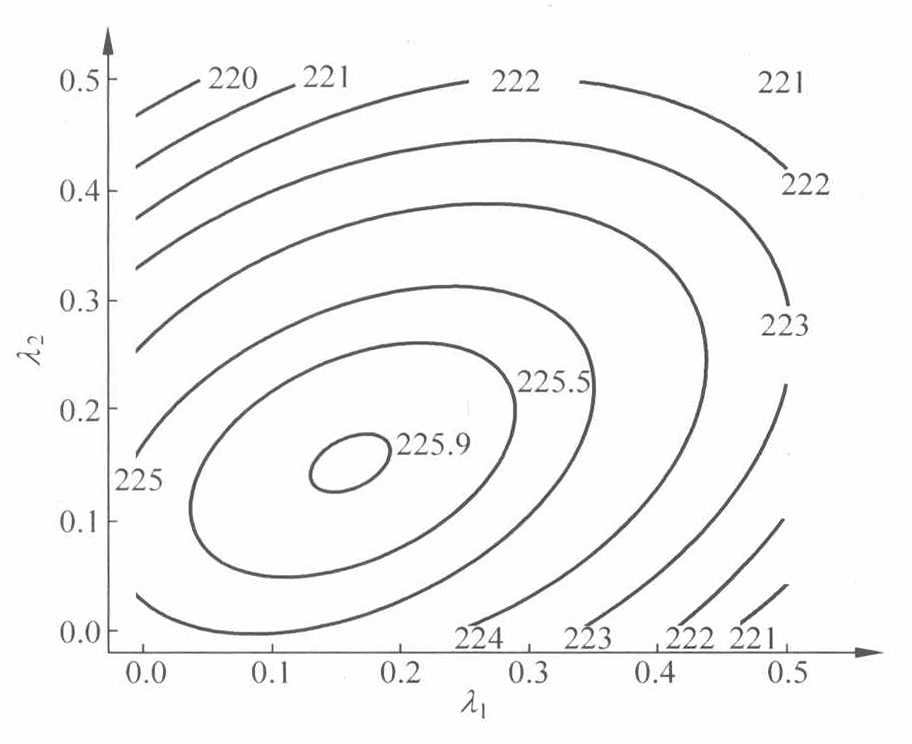
\includegraphics[width=77.2mm]{figs/fig_pg165_1.png}
\phantomsection\label{fig:4.15}\mvcap{图 4.15\quad 关于辐射量数据 $l(\lambda_1, \lambda_2)$ 的轮廓线图}
\end{mvfigure}

对这个二元情形“最好的”幂变换与考虑每个边缘分布所得到的幂变换没有显著差别. \hfill$\blacksquare$

正如我们在例 4.17 中所看到的, 使得每个边缘分布近似正态大致地等价于直接地处理二元分布并使得它近似正态. 通常对边缘分布比对联合分布更容易选择适当的变换.

如果数据中包含一些大的负值且具有单一的长尾, 应该应用更一般的变换(参见 Yeo 和 Johnson[14]).
\[
x^{(\lambda)} = \begin{cases} \{(x+1)^\lambda - 1\}/\lambda & x \geq 0, \lambda \neq 0 \\ \ln(x+1) & x \geq 0, \lambda = 0 \\ -\{(-x+1)^{2-\lambda} - 1\}/(2-\lambda) & x < 0, \lambda \neq 2 \\ -\ln(-x+1) & x < 0, \lambda = 2 \end{cases}
\]

\mvsub{练习}

\noindent 4.1\quad 设一个二元正态分布有 $\mu_1 = 1, \mu_2 = 3, \sigma_{11} = 2, \sigma_{22} = 1$ 和 $\rho_{12} = -0.8$.

\noindent (a) 写出二元正态密度.

\noindent (b) 把平方统计距离的表达式 $(\mathbf{x}-\boldsymbol{\mu})'\boldsymbol{\Sigma}^{-1}(\mathbf{x}-\boldsymbol{\mu})$ 写成 $x_1$ 和 $x_2$ 的二次函数.

\noindent 4.2\quad 设一个二元正态总体有 $\mu_1 = 0, \mu_2 = 2, \sigma_{11} = 2, \sigma_{22} = 1$ 和 $\rho_{12} = 0.5$.

\noindent (a) 写出二元正态密度.

\noindent (b) 把广义平方距离的表达式 $(\mathbf{x}-\boldsymbol{\mu})'\boldsymbol{\Sigma}^{-1}(\mathbf{x}-\boldsymbol{\mu})$ 写成 $x_1$ 和 $x_2$ 的函数.

\noindent (c) 确定含 $50\%$ 概率的常密度轮廓线(并画出草图).

\noindent 4.3\quad 设 $\mathbf{X}$ 服从 $\boldsymbol{\mu}' = [-3, 1, 4]$ 和
\[
\boldsymbol{\Sigma} = \begin{bmatrix} 1 & -2 & 0 \\ -2 & 5 & 0 \\ 0 & 0 & 2 \end{bmatrix}
\]
的 $N_3(\boldsymbol{\mu}, \boldsymbol{\Sigma})$, 下列各对随机变量中哪几对相互独立? 请解释.

%% ===== pg-166 =====

% ---- pg-166 （书页 154） ----

\noindent (a) $X_1$ 和 $X_2$

\noindent (b) $X_2$ 和 $X_3$

\noindent (c) $(X_1, X_2)$ 和 $X_3$

\noindent (d) $\dfrac{X_1 + X_2}{2}$ 和 $X_3$

\noindent (e) $X_2$ 和 $X_2 - \dfrac{5}{2}X_1 - X_3$

\noindent 4.4\quad 设 $\mathbf{X}$ 服从 $\boldsymbol{\mu}' = [2, -3, 1]$ 和
\[
\boldsymbol{\Sigma} = \begin{bmatrix} 1 & 1 & 1 \\ 1 & 3 & 2 \\ 1 & 2 & 2 \end{bmatrix}
\]
的 $N_3(\boldsymbol{\mu}, \boldsymbol{\Sigma})$,

\noindent (a) 求 $3X_1 - 2X_2 + X_3$ 的分布.

\noindent (b) 如果必要, 重新给变量标号, 并求一个 $2 \times 1$ 向量 $\mathbf{a}$, 使得 $X_2$ 与 $X_2 - \mathbf{a}'\begin{bmatrix} X_1 \\ X_3 \end{bmatrix}$ 相互独立.

\noindent 4.5\quad 对以下每一个概念作出详细说明.

\noindent (a) 对练习 4.2 中的联合分布给定 $X_2 = x_2$ 时 $X_1$ 的条件分布.

\noindent (b) 对练习 4.3 中的联合分布给定 $X_1 = x_1$ 和 $X_3 = x_3$ 时 $X_2$ 的条件分布.

\noindent (c) 对练习 4.4 中的联合分布给定 $X_1 = x_1$ 和 $X_2 = x_2$ 时 $X_3$ 的条件分布.

\noindent 4.6\quad 设 $\mathbf{X}$ 服从 $N_3(\boldsymbol{\mu}, \boldsymbol{\Sigma})$ 分布, 其中 $\boldsymbol{\mu}' = [1, -1, 2]$,
\[
\boldsymbol{\Sigma} = \begin{bmatrix} 4 & 0 & -1 \\ 0 & 5 & 0 \\ -1 & 0 & 2 \end{bmatrix}
\]
下列各对随机变量中哪几对相互独立? 试说明.

\noindent (a) $X_1$ 和 $X_2$

\noindent (b) $X_1$ 和 $X_3$

\noindent (c) $X_2$ 和 $X_3$

\noindent (d) $(X_1, X_3)$ 和 $X_2$

\noindent (e) $X_1$ 和 $X_1 + 3X_2 - 2X_3$

\noindent 4.7\quad 参看练习 4.6 详细说明以下每一个概念.

\noindent (a) 给定 $X_3 = x_3$ 时 $X_1$ 的条件分布.

\noindent (b) 给定 $X_2 = x_2$ 和 $X_3 = x_3$ 时 $X_1$ 的条件分布.

\noindent 4.8\quad (一个有正态边缘的非正态二元分布的例子)$X_1$ 服从 $N(0, 1)$, 且
\[
X_2 = \begin{cases} -X_1 & \text{若 } -1 \leq X_1 \leq 1 \\ X_1 & \text{其他} \end{cases}
\]
证明下列命题:

\noindent (a) $X_2$ 也服从 $N(0, 1)$ 分布.

\noindent (b) $X_1$ 和 $X_2$ 不服从二元正态分布.

\noindent 提示:

\noindent (a) 由于 $X_1$ 服从 $N(0, 1)$, 对任意 $x$ 有 $P[-1 < X_1 \leq x] = P[-x \leq X_1 < 1]$. 当 $-1 < x_2 < 1$

%% ===== pg-167 =====

时, $P[X_{2}\le x_{2}]=P[X_{2}\le -1]+P[-1<X_{2}\le x_{2}]=P[X_{1}\le -1]+P[-1<-X_{1}\le x_{2}]=P[X_{1}\le -1]+P[-x_{2}\le X_{1}<1]$. 然而用本提示开头的对称性论点有 $P[-x_{2}\le X_{1}<1]=P[-1<X_{1}\le x_{2}]$, 因此 $P[X_{2}\le x_{2}]=P[X_{1}\le -1]+P[-1<X_{1}\le x_{2}]=P[X_{1}\le x_{2}]$ 是一个标准正态概率.

(b) 考虑线性组合 $X_{1}-X_{2}$, 它等于 0 且概率 $P[|X_{1}|>1]=0.3174$.

4.9\quad 参看练习 4.8, 但用 $c$ 替换分割点 1 以更改结构, 得到
\[
X_{2}=\begin{cases}-X_{1} & \text{若 } -c\le X_{1}\le c\\[2pt] X_{1} & \text{其他}\end{cases}
\]
证明可以选到 $c$, 使得 $\operatorname{Cov}(X_{1},X_{2})=0$, 但两个随机变量却并不独立.

提示:

对于 $c=0$, 计算 $\operatorname{Cov}(X_{1},X_{2})=E[X_{1}(X_{1})]$.

对于很大的 $c$, 计算 $\operatorname{Cov}(X_{1},X_{2})\doteq E[X_{1}(-X_{1})]$.

4.10\quad 证明下列命题:

(a)
\[
\begin{vmatrix}\mathbf{A}&\mathbf{0}\\[2pt]\mathbf{0}'&\mathbf{B}\end{vmatrix}=|\mathbf{A}|\,|\mathbf{B}|
\]

(b)
\[
\begin{vmatrix}\mathbf{A}&\mathbf{C}\\[2pt]\mathbf{0}'&\mathbf{B}\end{vmatrix}=|\mathbf{A}|\,|\mathbf{B}|,\ \text{其中 } |\mathbf{A}|\ne 0
\]

提示:

(a)
\[
\begin{vmatrix}\mathbf{A}&\mathbf{0}\\[2pt]\mathbf{0}'&\mathbf{B}\end{vmatrix}
=\begin{vmatrix}\mathbf{A}&\mathbf{0}\\[2pt]\mathbf{0}'&\mathbf{I}\end{vmatrix}
\begin{vmatrix}\mathbf{I}&\mathbf{0}\\[2pt]\mathbf{0}'&\mathbf{B}\end{vmatrix}
\]
将行列式 $\begin{vmatrix}\mathbf{I}&\mathbf{0}\\[2pt]\mathbf{0}'&\mathbf{B}\end{vmatrix}$ 按第一行展开 (见定义 2A.24), 产生一个 1 乘一个降低一阶的 $\mathbf{I}$ 的同样形式的行列式. 重复此过程, 直到得出 $1\times|\mathbf{B}|$. 类似的, 将
$\begin{vmatrix}\mathbf{A}&\mathbf{0}\\[2pt]\mathbf{0}'&\mathbf{I}\end{vmatrix}$ 按最后一行展开, 产生 $\begin{vmatrix}\mathbf{A}&\mathbf{0}\\[2pt]\mathbf{0}'&\mathbf{I}\end{vmatrix}=|\mathbf{A}|$.

(b)
\[
\begin{vmatrix}\mathbf{A}&\mathbf{C}\\[2pt]\mathbf{0}'&\mathbf{B}\end{vmatrix}
=\begin{vmatrix}\mathbf{A}&\mathbf{0}\\[2pt]\mathbf{0}'&\mathbf{B}\end{vmatrix}
\begin{vmatrix}\mathbf{I}&\mathbf{A}^{-1}\mathbf{C}\\[2pt]\mathbf{0}'&\mathbf{I}\end{vmatrix}
\]
但将行列式 $\begin{vmatrix}\mathbf{I}&\mathbf{A}^{-1}\mathbf{C}\\[2pt]\mathbf{0}'&\mathbf{I}\end{vmatrix}$ 按最后一行展开, 给出
$\begin{vmatrix}\mathbf{I}&\mathbf{A}^{-1}\mathbf{C}\\[2pt]\mathbf{0}'&\mathbf{I}\end{vmatrix}=1$. 再利用 (a) 的结果.

4.11\quad 若 $\mathbf{A}$ 是方阵, 证明
\[
\begin{aligned}
|\mathbf{A}|&=|\mathbf{A}_{22}|\,|\mathbf{A}_{11}-\mathbf{A}_{12}\mathbf{A}_{22}^{-1}\mathbf{A}_{21}| &&\text{对 } |\mathbf{A}_{22}|\ne 0\\
&=|\mathbf{A}_{11}|\,|\mathbf{A}_{22}-\mathbf{A}_{21}\mathbf{A}_{11}^{-1}\mathbf{A}_{12}| &&\text{对 } |\mathbf{A}_{11}|\ne 0
\end{aligned}
\]

提示: 将 $\mathbf{A}$ 分块并证明
\[
\begin{bmatrix}\mathbf{I}&-\mathbf{A}_{12}\mathbf{A}_{22}^{-1}\\[4pt]\mathbf{0}'&\mathbf{I}\end{bmatrix}
\begin{bmatrix}\mathbf{A}_{11}&\mathbf{A}_{12}\\[4pt]\mathbf{A}_{21}&\mathbf{A}_{22}\end{bmatrix}
\begin{bmatrix}\mathbf{I}&\mathbf{0}\\[4pt]-\mathbf{A}_{22}^{-1}\mathbf{A}_{21}&\mathbf{I}\end{bmatrix}
=\begin{bmatrix}\mathbf{A}_{11}-\mathbf{A}_{12}\mathbf{A}_{22}^{-1}\mathbf{A}_{21}&\mathbf{0}\\[4pt]\mathbf{0}'&\mathbf{A}_{22}\end{bmatrix}
\]
对这个等式的两边取行列式, 再对左边第 1 个和第 3 个行列式以及右边的行列式利用练习 4.10 的结果. 对 $|\mathbf{A}|$ 的第 2 个等式考虑
\[
\begin{bmatrix}\mathbf{I}&\mathbf{0}\\[4pt]-\mathbf{A}_{21}\mathbf{A}_{11}^{-1}&\mathbf{I}\end{bmatrix}
\begin{bmatrix}\mathbf{A}_{11}&\mathbf{A}_{12}\\[4pt]\mathbf{A}_{21}&\mathbf{A}_{22}\end{bmatrix}
\]

%% ===== pg-168 =====

\[
\begin{bmatrix}\mathbf{I}&-\mathbf{A}_{11}^{-1}\mathbf{A}_{12}\\[4pt]\mathbf{0}'&\mathbf{I}\end{bmatrix}
=\begin{bmatrix}\mathbf{A}_{11}&\mathbf{0}\\[4pt]\mathbf{0}'&\mathbf{A}_{22}-\mathbf{A}_{21}\mathbf{A}_{11}^{-1}\mathbf{A}_{12}\end{bmatrix}
\]

4.12\quad 若 $\mathbf{A}$ 为对称矩阵, 证明
\[
\mathbf{A}^{-1}=\begin{bmatrix}\mathbf{I}&\mathbf{0}\\[4pt]-\mathbf{A}_{22}^{-1}\mathbf{A}_{21}&\mathbf{I}\end{bmatrix}
\begin{bmatrix}(\mathbf{A}_{11}-\mathbf{A}_{12}\mathbf{A}_{22}^{-1}\mathbf{A}_{21})^{-1}&\mathbf{0}\\[4pt]\mathbf{0}'&\mathbf{A}_{22}^{-1}\end{bmatrix}
\begin{bmatrix}\mathbf{I}&-\mathbf{A}_{12}\mathbf{A}_{22}^{-1}\\[4pt]\mathbf{0}'&\mathbf{I}\end{bmatrix}
\]
因此, $(\mathbf{A}_{11}-\mathbf{A}_{12}\mathbf{A}_{22}^{-1}\mathbf{A}_{21})^{-1}$ 是 $\mathbf{A}^{-1}$ 的左上角的块.

提示: 用 $\begin{bmatrix}\mathbf{I}&-\mathbf{A}_{12}\mathbf{A}_{22}^{-1}\\[2pt]\mathbf{0}'&\mathbf{I}\end{bmatrix}^{-1}$ 左乘练习 4.11 提示中的表达式, 并用 $\begin{bmatrix}\mathbf{I}&\mathbf{0}\\[2pt]-\mathbf{A}_{22}^{-1}\mathbf{A}_{21}&\mathbf{I}\end{bmatrix}^{-1}$ 右乘该式, 最后对所得结果取逆.

4.13\quad 若 $|\boldsymbol{\Sigma}|\ne 0$,

(a) 检验 $|\boldsymbol{\Sigma}|=|\boldsymbol{\Sigma}_{22}|\,|\boldsymbol{\Sigma}_{11}-\boldsymbol{\Sigma}_{12}\boldsymbol{\Sigma}_{22}^{-1}\boldsymbol{\Sigma}_{21}|$ (注意, $|\boldsymbol{\Sigma}|$ 可以表示成来自边缘分布和条件分布两部分的乘积).

(b) 检验
\begin{align*}
(\mathbf{x}-\boldsymbol{\mu})'\boldsymbol{\Sigma}^{-1}(\mathbf{x}-\boldsymbol{\mu})
&=\Bigl[\mathbf{x}_{1}-\boldsymbol{\mu}_{1}-\boldsymbol{\Sigma}_{12}\boldsymbol{\Sigma}_{22}^{-1}(\mathbf{x}_{2}-\boldsymbol{\mu}_{2})\Bigr]'\\
&\quad\times(\boldsymbol{\Sigma}_{11}-\boldsymbol{\Sigma}_{12}\boldsymbol{\Sigma}_{22}^{-1}\boldsymbol{\Sigma}_{21})^{-1}\Bigl[\mathbf{x}_{1}-\boldsymbol{\mu}_{1}-\boldsymbol{\Sigma}_{12}\boldsymbol{\Sigma}_{22}^{-1}(\mathbf{x}_{2}-\boldsymbol{\mu}_{2})\Bigr]\\
&\quad+(\mathbf{x}_{2}-\boldsymbol{\mu}_{2})'\boldsymbol{\Sigma}_{22}^{-1}(\mathbf{x}_{2}-\boldsymbol{\mu}_{2})
\end{align*}
(于是, 联合密度指数可以写成对应于来自边缘分布和条件分布的两项贡献之和.)

(c) 给定 (a) 和 (b) 的结果, 指出 $\mathbf{X}_{2}$ 的边缘分布和 $\mathbf{X}_{1}|\mathbf{X}_{2}=\mathbf{x}_{2}$ 下的条件分布.

提示:

(a) 应用练习 4.11.

(b) 注意到练习 4.12, 我们可以将 $(\mathbf{x}-\boldsymbol{\mu})'\boldsymbol{\Sigma}^{-1}(\mathbf{x}-\boldsymbol{\mu})$ 写做
\[
\begin{bmatrix}\mathbf{x}_{1}-\boldsymbol{\mu}_{1}\\[4pt]\mathbf{x}_{2}-\boldsymbol{\mu}_{2}\end{bmatrix}'
\begin{bmatrix}\mathbf{I}&\mathbf{0}\\[4pt]-\boldsymbol{\Sigma}_{22}^{-1}\boldsymbol{\Sigma}_{21}&\mathbf{I}\end{bmatrix}
\begin{bmatrix}(\boldsymbol{\Sigma}_{11}-\boldsymbol{\Sigma}_{12}\boldsymbol{\Sigma}_{22}^{-1}\boldsymbol{\Sigma}_{21})^{-1}&\mathbf{0}\\[4pt]\mathbf{0}'&\boldsymbol{\Sigma}_{22}^{-1}\end{bmatrix}
\times\begin{bmatrix}\mathbf{I}&-\boldsymbol{\Sigma}_{12}\boldsymbol{\Sigma}_{22}^{-1}\\[4pt]\mathbf{0}'&\mathbf{I}\end{bmatrix}
\begin{bmatrix}\mathbf{x}_{1}-\boldsymbol{\mu}_{1}\\[4pt]\mathbf{x}_{2}-\boldsymbol{\mu}_{2}\end{bmatrix}
\]
如果我们组合乘积, 使得
\[
\begin{bmatrix}\mathbf{I}&-\boldsymbol{\Sigma}_{12}\boldsymbol{\Sigma}_{22}^{-1}\\[4pt]\mathbf{0}'&\mathbf{I}\end{bmatrix}
\begin{bmatrix}\mathbf{x}_{1}-\boldsymbol{\mu}_{1}\\[4pt]\mathbf{x}_{2}-\boldsymbol{\mu}_{2}\end{bmatrix}
=\begin{bmatrix}\mathbf{x}_{1}-\boldsymbol{\mu}_{1}-\boldsymbol{\Sigma}_{12}\boldsymbol{\Sigma}_{22}^{-1}(\mathbf{x}_{2}-\boldsymbol{\mu}_{2})\\[4pt]\mathbf{x}_{2}-\boldsymbol{\mu}_{2}\end{bmatrix}
\]
便得所需结果.

4.14\quad 若 $\mathbf{X}$ 的分布为 $N_{p}(\boldsymbol{\mu},\boldsymbol{\Sigma})$ 且 $|\boldsymbol{\Sigma}|\ne 0$, 试证明若 $\boldsymbol{\Sigma}_{12}=\mathbf{0}_{(q\times(p-q))}$, 则联合密度可写成 $\mathbf{X}_{1\,(q\times 1)}$ 和 $\mathbf{X}_{2\,((p-q)\times 1)}$ 的两个边缘密度的乘积.

提示: 用分块乘法证明 $\begin{bmatrix}\boldsymbol{\Sigma}_{11}^{-1}&\mathbf{0}\\[2pt]\mathbf{0}'&\boldsymbol{\Sigma}_{22}^{-1}\end{bmatrix}$ 为 $\boldsymbol{\Sigma}=\begin{bmatrix}\boldsymbol{\Sigma}_{11}&\mathbf{0}\\[2pt]\mathbf{0}'&\boldsymbol{\Sigma}_{22}\end{bmatrix}$ 的逆. 然后写出
\begin{align*}
(\mathbf{x}-\boldsymbol{\mu})'\boldsymbol{\Sigma}^{-1}(\mathbf{x}-\boldsymbol{\mu})
&=\bigl[(\mathbf{x}_{1}-\boldsymbol{\mu}_{1})',(\mathbf{x}_{2}-\boldsymbol{\mu}_{2})'\bigr]
\begin{bmatrix}\boldsymbol{\Sigma}_{11}^{-1}&\mathbf{0}\\[4pt]\mathbf{0}'&\boldsymbol{\Sigma}_{22}^{-1}\end{bmatrix}
\begin{bmatrix}\mathbf{x}_{1}-\boldsymbol{\mu}_{1}\\[4pt]\mathbf{x}_{2}-\boldsymbol{\mu}_{2}\end{bmatrix}\\
&=(\mathbf{x}_{1}-\boldsymbol{\mu}_{1})'\boldsymbol{\Sigma}_{11}^{-1}(\mathbf{x}_{1}-\boldsymbol{\mu}_{1})+(\mathbf{x}_{2}-\boldsymbol{\mu}_{2})'\boldsymbol{\Sigma}_{22}^{-1}(\mathbf{x}_{2}-\boldsymbol{\mu}_{2})
\end{align*}
由练习 4.10(a) 注意到 $|\boldsymbol{\Sigma}|=|\boldsymbol{\Sigma}_{11}|\,|\boldsymbol{\Sigma}_{22}|$, 便可分解为联合密度.

4.15\quad 证明 $\sum\limits_{j=1}^{n}(\mathbf{x}_{j}-\bar{\mathbf{x}})(\bar{\mathbf{x}}-\boldsymbol{\mu})'$ 和 $\sum\limits_{j=1}^{n}(\bar{\mathbf{x}}-\boldsymbol{\mu})(\mathbf{x}_{j}-\bar{\mathbf{x}})'$ 二者皆为 $p\times p$ 的零矩阵, 此处

%% ===== pg-169 =====

$\mathbf{x}_{j}'=[x_{j1},x_{j2},\cdots,x_{jp}],j=1,2,\cdots,n$ 和
\[
\bar{\mathbf{x}}=\frac{1}{n}\sum_{j=1}^{n}\mathbf{x}_{j}
\]

4.16\quad 设 $\mathbf{X}_{1},\mathbf{X}_{2},\mathbf{X}_{3}$ 和 $\mathbf{X}_{4}$ 是独立 $N_{p}(\boldsymbol{\mu},\boldsymbol{\Sigma})$ 随机向量.

(a) 对以下两个随机向量求边缘分布:
\[
\mathbf{V}_{1}=\frac{1}{4}\mathbf{X}_{1}-\frac{1}{4}\mathbf{X}_{2}+\frac{1}{4}\mathbf{X}_{3}-\frac{1}{4}\mathbf{X}_{4}
\]
\[
\mathbf{V}_{2}=\frac{1}{4}\mathbf{X}_{1}+\frac{1}{4}\mathbf{X}_{2}-\frac{1}{4}\mathbf{X}_{3}-\frac{1}{4}\mathbf{X}_{4}
\]

(b) 求 (a) 中定义的随机向量 $\mathbf{V}_{1}$ 和 $\mathbf{V}_{2}$ 的联合密度.

4.17\quad 设 $\mathbf{X}_{1},\mathbf{X}_{2},\mathbf{X}_{3},\mathbf{X}_{4}$ 和 $\mathbf{X}_{5}$ 是有均值向量 $\boldsymbol{\mu}$ 和协方差矩阵 $\boldsymbol{\Sigma}$ 的独立同分布随机向量, 试对这些随机向量的两个线性组合
\[
\frac{1}{5}\mathbf{X}_{1}+\frac{1}{5}\mathbf{X}_{2}+\frac{1}{5}\mathbf{X}_{3}+\frac{1}{5}\mathbf{X}_{4}+\frac{1}{5}\mathbf{X}_{5}
\]
和
\[
\mathbf{X}_{1}-\mathbf{X}_{2}+\mathbf{X}_{3}-\mathbf{X}_{4}+\mathbf{X}_{5}
\]
分别求均值向量和协方差矩阵, 并求这两个线性组合之间的协方差.

4.18\quad 试根据来自二维正态总体的随机样本
\[
\mathbf{X}=\begin{bmatrix}3&6\\4&4\\5&7\\4&7\end{bmatrix}
\]
求 $2\times 1$ 均值向量 $\boldsymbol{\mu}$ 和 $2\times 2$ 协方差矩阵 $\boldsymbol{\Sigma}$ 的极大似然估计.

4.19\quad 设 $\mathbf{X}_{1},\mathbf{X}_{2},\cdots,\mathbf{X}_{20}$ 为来自总体 $N_{6}(\boldsymbol{\mu},\boldsymbol{\Sigma})$, 容量 $n=20$ 的一个随机样本, 试对下列分布给出完整说明:

(a) $(\mathbf{X}_{1}-\boldsymbol{\mu})'\boldsymbol{\Sigma}^{-1}(\mathbf{X}_{1}-\boldsymbol{\mu})$ 的分布.

(b) $\bar{\mathbf{X}}$ 和 $\sqrt{n}(\bar{\mathbf{X}}-\boldsymbol{\mu})$ 的分布.

(c) $(n-1)\mathbf{S}$ 的分布.

4.20\quad 对练习 4.19 中的随机变量 $\mathbf{X}_{1},\mathbf{X}_{2},\cdots,\mathbf{X}_{20}$, 详细说明以下情况中 $\mathbf{B}(19\mathbf{S})\mathbf{B}'$ 的分布:

(a) $\mathbf{B}=\begin{bmatrix}1&-1/2&-1/2&0&0&0\\0&0&0&-1/2&-1/2&1\end{bmatrix}$

(b) $\mathbf{B}=\begin{bmatrix}1&0&0&0&0&0\\0&0&1&0&0&0\end{bmatrix}$

4.21\quad 设 $\mathbf{X}_{1},\cdots,\mathbf{X}_{60}$ 为来自均值为 $\boldsymbol{\mu}$ 和协方差为 $\boldsymbol{\Sigma}$ 的 4 维正态分布的随机样本, 其容量为 60. 试对下列各项给出完整说明:

(a) $\bar{\mathbf{X}}$ 的分布.

(b) $(\mathbf{X}_{1}-\boldsymbol{\mu})'\boldsymbol{\Sigma}^{-1}(\mathbf{X}_{1}-\boldsymbol{\mu})$ 的分布.

(c) $n(\bar{\mathbf{X}}-\boldsymbol{\mu})'\boldsymbol{\Sigma}^{-1}(\bar{\mathbf{X}}-\boldsymbol{\mu})$ 的分布.

(d) $n(\bar{\mathbf{X}}-\boldsymbol{\mu})'\mathbf{S}^{-1}(\bar{\mathbf{X}}-\boldsymbol{\mu})$ 的近似分布.

4.22\quad 设 $\mathbf{X}_{1},\mathbf{X}_{2},\cdots,\mathbf{X}_{75}$ 为来自均值为 $\boldsymbol{\mu}$, 协方差矩阵为 $\boldsymbol{\Sigma}$ 的总体分布的随机样本, 下面每个统计量的近似分布是什么?

%% ===== pg-170 =====

(a) $\bar{\mathbf{X}}$

(b) $n(\bar{\mathbf{X}}-\boldsymbol{\mu})'\mathbf{S}^{-1}(\bar{\mathbf{X}}-\boldsymbol{\mu})$

4.23\quad 考虑 1996—2005 年间道琼斯工业股票价格指数的年回报率 (包括红利). 这些数据乘以 100, 便是 $-0.6,3.1,25.3,-16.8,-7.1,-6.2,25.2,22.6$ 和 $26.0$. 试利用这 9 个观测值完成下列问题.

(a) 作一个 Q-Q 图. 这些数据看起来是否正态分布? 请解释.

(b) 完成一个基于相关系数 $r_{Q}$ 的正态性检验 [见\hyperref[eq:4-31]{式(4-31)}]. 显著性水平取 $\alpha=0.10$.

4.24\quad 练习 1.4 给出了 2005 年 4 月 10 家最大公司三个变量的数据. 试对销售额 $(x_{1})$ 和利润 $(x_{2})$ 的数据

(a) 作 Q-Q 图. 这些数据看起来是否正态分布? 请解释.

(b) 完成一个基于相关系数 $r_{Q}$ 的正态性检验 [见\hyperref[eq:4-31]{式(4-31)}]. 显著性水平取 $\alpha=0.10$. 这些检验结果能否证实 (a) 中的结果?

4.25\quad 参看练习 1.4 中 10 家最大公司的数据. 利用所有三个变量作卡方图. 卡方分位数为 $0.3518$ $0.7978$ $1.2125$ $1.6416$ $2.1095$ $2.6430$ $3.2831$ $4.1083$ $5.3170$ $7.8147$

4.26\quad 练习 1.2 给出 $n=10$ 辆旧车的车龄 $x_{1}$ (年) 和销售价格 $x_{2}$ (千美元). 这些数据如下:

\begin{mvtable}
\begin{tabular}{lrrrrrrrrrr}
\toprule
$x_{1}$&1&2&3&4&5&6&7&8&9&11\\
\midrule
$x_{2}$&18.95&19.00&17.95&15.54&14.00&12.95&8.94&7.49&6.00&3.99\\
\bottomrule
\end{tabular}
\end{mvtable}

(a) 利用练习 1.2 的结果计算平方统计距离
\[
(\mathbf{x}_{j}-\bar{\mathbf{x}})'\mathbf{S}^{-1}(\mathbf{x}_{j}-\bar{\mathbf{x}}),j=1,2,\cdots,10,\quad\text{其中 } \mathbf{x}_{j}'=[x_{j1},x_{j2}].
\]

(b) 利用 (a) 中得出的距离, 确定落在二维正态分布估计的 $50\%$ 概率轮廓线之内的诸观测值所占的比例.

(c) 将 (a) 中的距离排序并作卡方图.

(d) 给定 (b) 和 (c) 的结果, 这些数据是否接近二维正态分布? 请解释.

4.27\quad 考虑例 4.10 的辐射数据 (炉门关闭). 对这些数据的自然对数作 Q-Q 图 [注意自然对数变换对应\hyperref[eq:4-34]{式(4-34)} 中的 $\lambda=0$]. 这些自然对数看起来是否呈正态分布? 将你的结果同\hyperref[fig:4.13]{图 4.13} 相比较. 在这种情况下, 选择 $\lambda=1/4$ 或 $\lambda=0$ 是否会产生很大差别?

\textbf{下面的练习需要使用计算机.}

4.28\quad 考虑\hyperref[tab:1.5]{表 1.5} 中所给的空气污染数据, 对太阳辐射测量值作 Q-Q 图, 并根据相关系数 $r_{Q}$ 完成正态性检验 (见\hyperref[eq:4-31]{式(4-31)}). 取 $\alpha=0.05$ 并利用\hyperref[tab:4.2]{表 4.2} 中对应于 $n=40$ 的 $r_{Q}$ 值.

4.29\quad 用\hyperref[tab:1.5]{表 1.5} 中所给的空气污染数据, 考察 $X_{5}=\mathrm{NO}_{2}$ 和 $X_{6}=\mathrm{O}_{3}$ 这对变量的二维正态性.

(a) 计算统计距离 $(\mathbf{x}_{j}-\bar{\mathbf{x}})'\mathbf{S}^{-1}(\mathbf{x}_{j}-\bar{\mathbf{x}}),j=1,2,\cdots,42$, 其中 $\mathbf{x}_{j}'=[x_{j5},x_{j6}]$.

(b) 确定落在二维正态分布的大约 $50\%$ 概率轮廓线之内的观测值 $\mathbf{x}_{j}'=[x_{j5},x_{j6}],j=1,2,\cdots,42$, 所占的比例.

(c) 用 (a) 中排序距离作卡方图.

4.30\quad 考虑练习 4.26 中旧车数据.

(a) 确定能使 $x_{1}$ 值接近正态分布的幂变换 $\hat{\lambda}_{1}$. 对变换后的数据作 Q-Q 图.

%% ===== pg-171 =====

(b) 确定能使 $x_{2}$ 值接近正态分布的幂变换 $\hat{\lambda}_{2}$. 对变换后的数据作 Q-Q 图.

(c) 利用\hyperref[eq:4-40]{式(4-40)}, 确定能使 $[x_{1},x_{2}]$ 值服从联合正态分布的幂变换 $\hat{\boldsymbol{\lambda}}'=[\hat{\lambda}_{1},\hat{\lambda}_{2}]$. 将此结果同 (a) 和 (b) 中得出的结果进行比较.

4.31\quad 试对\hyperref[tab:1.6]{表 1.6} 中的多发性硬化症数据考察变量 $X_{1},X_{2},\cdots,X_{5}$ 观测值的边缘正态性. 对非多发硬化和多发硬化症两组数据分别进行处理. 可以采用你认为合适的任何处理方法, 包括变换.

4.32\quad 试对\hyperref[tab:1.7]{表 1.7} 中射线疗法数据考察变量 $X_{1},X_{2},\cdots,X_{6}$ 观测值的边缘正态性. 可以采用你认为合适的包括变换在内的任何方法.

4.33\quad 试对\hyperref[tab:4.3]{表 4.3} 中的数据考察变量 $X_{1},X_{2},X_{3}$ 和 $X_{4}$ 观测值的边缘和二维的正态性.

4.34\quad 考察\hyperref[tab:1.8]{表 1.8} 中骨骼无机物含量数据的边缘和二维的正态性.

4.35\quad 考察\hyperref[tab:1.2]{表 1.2} 中纸张质量测量值数据的边缘和多元的正态性.

4.36\quad 考察\hyperref[tab:1.9]{表 1.9} 中女子全国和地区径赛记录数据的边缘和多元的正态性.

4.37\quad 参看练习 1.18. 将\hyperref[tab:1.9]{表 1.9} 中女子径赛记录转变为以米每秒度量的速度. 考察这些速度数据的边缘和多元正态性.

4.38\quad 考察\hyperref[tab:1.10]{表 1.10} 中公牛数据的边缘和多元正态性. 只考虑变量 YrHgt, FtFrBody, PrctFFB, BkFat, SaleHt, 和 SaleWt.

4.39\quad \hyperref[tab:4.6]{表 4.6} 中的数据 (参见心理概况数据: www.prenhall.com/statistics) 是通过对秘鲁青年 (年龄 15,16 和 17 岁) 进行心理测试打分产生的 130 个观测值. 对这些青年, 性别 (男性$=1$, 女性$=2$) 和社会经济地位 (低$=1$, 中等$=2$) 也被记录下来了. 这些分值被累加到下列 5 个度量分值中, 这 5 个量分别为独立性 (indep)、支撑力 (supp)、仁爱心 (benev)、顺从性 (conform) 和领导能力 (leader).

\begin{mvtable}
\phantomsection\label{tab:4.6}\mvtabcap{表 4.6\quad 心理概况数据}
\begin{tabular}{rrrrrrr}
\toprule
独立性&支撑力&仁爱心&顺从性&领导能力&性别&地位\\
\midrule
27&13&14&20&11&2&1\\
12&13&24&25&6&2&1\\
14&20&15&16&7&2&1\\
18&20&17&12&6&2&1\\
9&22&22&21&6&2&1\\
$\vdots$&$\vdots$&$\vdots$&$\vdots$&$\vdots$&$\vdots$&$\vdots$\\
10&11&26&17&10&1&2\\
14&12&14&11&29&1&2\\
19&11&23&18&13&2&2\\
27&19&22&7&9&2&2\\
10&17&22&22&8&2&2\\
\bottomrule
\end{tabular}

\vspace{2pt}
{\zihao{6}资料来源: 数据经 C. Soto 许可使用.}
\end{mvtable}

(a) 检验独立性、支撑力、仁爱心、顺从性和领导能力这些变量中的每一个的边缘正态性.

(b) 利用所有的 5 个变量, 检验其多元正态性.

(c) 参照 (a), 对于那些非正态变量, 确定一个变换使它们更加接近正态.

4.40\quad 考虑练习 1.27 中的国家公园数据.

(a) 对原始数据的散点图中所有可能的离群值作出评论.

%% ===== pg-172 =====

(b) 确定幂变换 $\hat{\lambda}_{1}$ 使变量 $x_{1}$ 接近正态. 画出变换后观测值的 Q-Q 图.

(c) 确定幂变换 $\hat{\lambda}_{2}$ 使变量 $x_{2}$ 接近正态. 画出变换后观测值的 Q-Q 图.

(d) 用\hyperref[eq:4-40]{式(4-40)} 确定接近二元正态的幂变换.

4.41\quad 考虑练习 3.20 中的扫雪数据.

(a) 对原始数据的散点图中所有可能的离群值作出评论.

(b) 确定幂变换 $\hat{\lambda}_{1}$ 使变量 $x_{1}$ 接近正态. 画出变换后观测值的 Q-Q 图.

(c) 确定幂变换 $\hat{\lambda}_{2}$ 使变量 $x_{2}$ 接近正态. 画出变换后观测值的 Q-Q 图.

(d) 用\hyperref[eq:4-40]{式(4-40)} 确定接近二元正态的幂变换.

\phantomsection\label{bib:4}
\section*{参考文献}

\begin{enumerate}[leftmargin=2em,itemsep=2pt]
\item Anderson, T. W. \textit{An Introduction to Multivariate Statistical Analysis} (3rd ed.). New York: John Wiley, 2003.
\item Andrews, D. F., R. Gnanadesikan, and J. L. Warner. “Transformations of Multivariate Data.” \textit{Biometrics}, \textbf{27}, no. 4 (1971), 825--840.
\item Box, G. E. P., and D. R. Cox. “An Analysis of Transformations” (with discussion). \textit{Journal of the Royal Statistical Society (B)}, \textbf{26}, no. 2 (1964), 211--252.
\item Daniel, C. and F. S. Wood, \textit{Fitting Equations to Data: Computer Analysis of Multifactor Data}. New York: John Wiley, 1980.
\item Filliben, J. J. “The Probability Plot Correlation Coefficient Test for Normality.” \textit{Technometrics}, \textbf{17}, no. 1 (1975), 111--117.
\item Gnanadesikan, R. \textit{Methods for Statistical Data Analysis of Multivariate Observations} (2nd ed.). New York: Wiley-Interscience, 1977.
\item Hawkins, D. M. \textit{Identification of Outliers}. London, UK: Chapman and Hall, 1980.
\item Hernandez, F., and R. A. Johnson. “The Large-Sample Behavior of Transformations to Normality.” \textit{Journal of the American Statistical Association}, \textbf{75}, no. 372 (1980), 855--861.
\item Hogg, R. V., Craig, A. T. and J. W. Mckean \textit{Introduction to Mathematical Statistics} (6th ed.). Upper Saddle River, N.J.: Prentice Hall, 2004.
\item Looney, S. W., and T. R. Gulledge, Jr. “Use of the Correlation Coefficient with Normal Probability Plots.” \textit{The American Statistician}, \textbf{39}, no. 1 (1985), 75--79.
\item Mardia, K. V., Kent, J. T. and J. M. Bibby. \textit{Multivariate Analysis} (Paperback). London: Academic Press, 2003.
\item Shapiro, S. S., and M. B. Wilk. “An Analysis of Variance Test for Normality (Complete Samples).” \textit{Biometrika}, \textbf{52}, no. 4 (1965), 591--611.
\item Verrill, S., and R. A. Johnson. “Tables and Large-Sample Distribution Theory for Censored-Data Correlation Statistics for Testing Normality.” \textit{Journal of the American Statistical Association}, \textbf{83}, no. 404 (1988), 1192--1197.
\item Yeo, I. and R. A. Johnson “A New Family of Power Transformations to Improve Normality or Symmetry.” \textit{Biometrika}, \textbf{87}, no. 4 (2000), 954--959.
\item Zehna, P. “Invariance of Maximum Likelihood Estimators.” \textit{Annals of Mathematical Statistics}, \textbf{37}, no. 3 (1966), 744.
\end{enumerate}

%% ===== pg-173 =====

% ---- pg-173 （书页 161） ----

\chapter{多元正态分布的统计推断}
\phantomsection\label{chap:5}

\section{引言}
\phantomsection\label{sec:5.1}

本书从这一章起开始转入多元统计学的方法论. 我们将利用前面第 1 章至第 4 章的各种概念和结论建立数据分析的方法. 任何一种分析, 其大部分内容均与统计推断相联系, 即根据来自样本的信息得出有关总体的有效结论.

基于这一观点, 我们将集中讨论关于总体均值向量及其分量的统计推断问题. 虽然我们将从假设检验开始统计推断的讨论, 但我们的最终目的, 还是要基于联合置信域的形式给出均值向量诸分量的一个完整的统计分析.

多元分析的精髓之一, 就是必须对 $p$ 个相关变量同时进行分析. 我们将通过用本章中给出的方法来举例说明这一原理.

\section{\texorpdfstring{$\boldsymbol{\mu}_0$}{mu0} 作为正态总体均值的似真性}
\phantomsection\label{sec:5.2}

我们先回忆一下在一元统计理论中, 判断 $\mu_0$ 是否为总体均值 $\mu$ 的似真值的假设检验问题. 从假设检验的观点出发, 这个问题可归结为检验假设
\[
H_0: \mu = \mu_0, \qquad H_1: \mu \neq \mu_0
\]
这里 $H_0$ 为零假设, 而 $H_1$ 为(双边)备择假设. 设 $X_1, X_2, \cdots, X_n$ 为一从正态总体中抽取的随机样本, 那么, 合理的检验统计量为
\[
t = \frac{(\bar{X} - \mu_0)}{s/\sqrt{n}}
\]
其中 $\bar{X} = \dfrac{1}{n}\sum\limits_{i=1}^{n}X_i$, $s^2 = \dfrac{1}{n-1}\sum\limits_{i=1}^{n}(X_i - \bar{X})^2$.

这个检验统计量是自由度(d.f.)为 $n-1$ 的 $t$ 分布. 如果观测到的 $|t|$ 值超过自由度为 $n-1$ 的 $t$ 分布的某个特定百分位点的值, 则拒绝 $H_0$, 即 $\mu_0$ 不是 $\mu$ 的似真值.

当 $|t|$ 值较大时拒绝 $H_0$ 等价于 $t$ 的平方
\phantomsection\label{eq:5-1}
\begin{equation}
t^2 = \frac{(\bar{X} - \mu_0)^2}{s^2/n} = n(\bar{X} - \mu_0)(s^2)^{-1}(\bar{X} - \mu_0) \tag{5-1}
\end{equation}
较大时拒绝 $H_0$. 在\hyperref[eq:5-1]{式(5-1)}中, 变量 $t^2$ 为样本均值 $\bar{X}$ 到检验值 $\mu_0$ 的距离的平方. 距离的单位可用 $s/\sqrt{n}$ 或者 $\bar{X}$ 的估计标准差来表示. 一旦观测出 $\bar{X}$ 和 $s^2$, 则检验的原则为: 在显著性水平 $\alpha$ 下, 如果
\phantomsection\label{eq:5-2}
\begin{equation}
n(\bar{x} - \mu_0)(s^2)^{-1}(\bar{x} - \mu_0) > t_{n-1}^2(\alpha/2) \tag{5-2}
\end{equation}
则拒绝 $H_0$ 而接受 $H_1$, 其中 $t_{n-1}(\alpha/2)$ 代表自由度为 $n-1$ 的 $t$ 分布的上 $100(\alpha/2)$ 百分位数.

如果 $H_0$ 没有被拒绝, 那么我们就认为 $\mu_0$ 为正态总体均值的似真值. 然而, 问题是, 是否还

%% ===== pg-174 =====

% ---- pg-174 （书页 162） ----

有 $\mu$ 的其他值与数据相吻合呢? 回答是肯定的. 事实上, 总是存在正态总体均值的一个似真值集合. 从众所周知的检验假设 $H_0: \mu = \mu_0$, $H_1: \mu \neq \mu_0$ 的接受域与 $\mu$ 的置信区间之间的对应关系, 我们有

\{在显著性水平 $\alpha$ 下, $H_0: \mu = \mu_0$ 未被拒绝\} 或
\[
\left|\frac{\bar{x} - \mu_0}{s/\sqrt{n}}\right| \leq t_{n-1}(\alpha/2)
\]
等价于

\{$\mu_0$ 落在 $100(1-\alpha)\%$ 置信区间 $\bar{x} \pm t_{n-1}(\alpha/2)\dfrac{s}{\sqrt{n}}$ 内\} 或
\phantomsection\label{eq:5-3}
\begin{equation}
\bar{x} - t_{n-1}(\alpha/2)\frac{s}{\sqrt{n}} \leq \mu_0 \leq \bar{x} + t_{n-1}(\alpha/2)\frac{s}{\sqrt{n}} \tag{5-3}
\end{equation}
因此, 在水平 $\alpha$ 下, 没有被假设 $H_0: \mu = \mu_0$ 的检验拒绝的所有值 $\mu_0$ 构成了这个置信区间.

在样本尚未选出之前, \hyperref[eq:5-3]{式(5-3)}中的 $100(1-\alpha)\%$ 置信区间是一个随机区间, 因为该区间的两个端点依赖于随机变量 $\bar{X}$ 和 $s$, 该区间包含 $\mu$ 的概率为 $1-\alpha$; 在大量这样的独立区间中, 大约有 $100(1-\alpha)\%$ 的区间包含 $\mu$.

现在我们考虑对一给定的 $p \times 1$ 向量 $\boldsymbol{\mu}$, 判断它是否为多元正态分布均值的似真值的假设检验问题. 我们将采用对方所讨论的一元问题作类比推广的方法来处理这个问题.

\hyperref[eq:5-1]{式(5-1)}中平方距离的多元情形的一个自然推广形式是
\phantomsection\label{eq:5-4}
\begin{equation}
T^2 = (\bar{\mathbf{X}} - \boldsymbol{\mu}_0)'\left(\frac{1}{n}\mathbf{S}\right)^{-1}(\bar{\mathbf{X}} - \boldsymbol{\mu}_0) = n(\bar{\mathbf{X}} - \boldsymbol{\mu}_0)'\mathbf{S}^{-1}(\bar{\mathbf{X}} - \boldsymbol{\mu}_0) \tag{5-4}
\end{equation}
其中
\[
\bar{\mathbf{X}} = \frac{1}{n}\sum_{j=1}^{n}\mathbf{X}_j, \quad \mathbf{S} = \frac{1}{n-1}\sum_{j=1}^{n}(\mathbf{X}_j - \bar{\mathbf{X}})(\mathbf{X}_j - \bar{\mathbf{X}})', \quad \text{且 } \boldsymbol{\mu}_0 = \begin{bmatrix} \mu_{10} \\ \mu_{20} \\ \vdots \\ \mu_{p0} \end{bmatrix}
\]

统计量 $T^2$ 的分布最早是由多元分析的先驱者霍特林(Hotelling)得出的, 为纪念这位先驱者, 我们通常称该统计量为霍特林 $T^2$ 统计量. \hyperref[eq:5-4]{式(5-4)}中的 $(1/n)\mathbf{S}$ 为 $\bar{\mathbf{X}}$ 的协方差矩阵的估计量(见结论 3.1).

如果观察到的统计距离 $T^2$ 太大, 也就是说, $\bar{\mathbf{x}}$ 与 $\boldsymbol{\mu}_0$ 距离太远, 那么我们就拒绝假设 $H_0: \mu = \mu_0$. 需要指出的是, 在检验该假设时, 我们并不需要特殊的 $T^2$ 百分位数表, 这是因为
\phantomsection\label{eq:5-5}
\begin{equation}
T^2 \text{ 与 } \frac{(n-1)p}{(n-p)}F_{p, n-p} \text{ 同分布} \tag{5-5}
\end{equation}
其中 $F_{p, n-p}$ 为服从自由度为 $p$ 和 $n-p$ 的 $F$ 分布随机变量.

概括起来, 我们有如下结论:

\begin{mvbox}
设 $X_1, X_2, \cdots, X_n$ 为从总体 $N_p(\boldsymbol{\mu}, \boldsymbol{\Sigma})$ 中抽取的一随机样本. 记 $\bar{\mathbf{X}} = \dfrac{1}{n}\sum\limits_{j=1}^{n}\mathbf{X}_j$, $\mathbf{S} = \dfrac{1}{(n-1)}\sum\limits_{j=1}^{n}(\mathbf{X}_j - \bar{\mathbf{X}})(\mathbf{X}_j - \bar{\mathbf{X}})'$, 那么
\phantomsection\label{eq:5-6}
\begin{align}
\alpha &= P\left[T^2 > \frac{(n-1)p}{(n-p)}F_{p, n-p}(\alpha)\right] \nonumber \\
&= P\left[n(\bar{\mathbf{X}} - \boldsymbol{\mu})'\mathbf{S}^{-1}(\bar{\mathbf{X}} - \boldsymbol{\mu}) > \frac{(n-1)p}{(n-p)}F_{p, n-p}(\alpha)\right] \tag{5-6}
\end{align}
对所有 $\boldsymbol{\mu}$ 与 $\boldsymbol{\Sigma}$ 成立, 这里 $F_{p, n-p}(\alpha)$ 为 $F_{p, n-p}$ 分布的上 $100\alpha$ 百分位数.
\end{mvbox}

%% ===== pg-175 =====

从\hyperref[eq:5-6]{式(5-6)}可立即得到假设 $H_0: \boldsymbol{\mu}=\boldsymbol{\mu}_0$, $H_1: \boldsymbol{\mu}\neq\boldsymbol{\mu}_0$ 的一个检验方法. 若在显著性水平 $\alpha$ 下,

\phantomsection\label{eq:5-7}
\begin{equation}
T^2=n(\bar{\mathbf{x}}-\boldsymbol{\mu}_0)'\mathbf{S}^{-1}(\bar{\mathbf{x}}-\boldsymbol{\mu}_0)>\frac{(n-1)p}{(n-p)}F_{p,n-p}(\alpha) \tag{5-7}
\end{equation}

则拒绝 $H_0$ 而接受 $H_1$.

简要讨论一下 $T^2$ 分布的实质及其与一元检验统计量之间的对应关系, 有助于我们对 $T^2$ 分布的了解. 在 4.4 节中我们曾指出, 威沙特分布是 $\chi^2$ 分布的推广, 由于

\[
T^2=\sqrt{n}(\bar{\mathbf{X}}-\boldsymbol{\mu}_0)'\left(\frac{\sum_{j=1}^{n}(\mathbf{X}_j-\bar{\mathbf{X}})(\mathbf{X}_j-\bar{\mathbf{X}})'}{n-1}\right)^{-1}\sqrt{n}(\bar{\mathbf{X}}-\boldsymbol{\mu}_0)
\]

通过关系

\phantomsection\label{eq:5-8}
\begin{equation}
\begin{aligned}
T^2_{p,n-1}&=\begin{pmatrix}\text{多元正态}\\ \text{随机向量}\end{pmatrix}'\begin{pmatrix}\text{威沙特随机矩阵}\\ \text{自由度}\end{pmatrix}^{-1}\begin{pmatrix}\text{多元正态}\\ \text{随机向量}\end{pmatrix}\\
&=N_p(\mathbf{0},\boldsymbol{\Sigma})'\left[\frac{1}{n-1}W_{p,n-1}(\boldsymbol{\Sigma})\right]^{-1}N_p(\mathbf{0},\boldsymbol{\Sigma})
\end{aligned} \tag{5-8}
\end{equation}

与正态随机向量 $N_p(\mathbf{0},\boldsymbol{\Sigma})$ 及威沙特随机矩阵 $W_{p,n-1}(\boldsymbol{\Sigma})$ 相联系, 所以, $T^2$ 与一元情形下的

\[
t^2=\sqrt{n}(\bar{X}-\mu_0)(s^2)^{-1}\sqrt{n}(\bar{X}-\mu_0)
\]

或

\[
t^2_{n-1}=\left(\text{正态随机变量}\right)\left(\frac{\chi^2\text{ 随机变量}}{\text{自由度}}\right)^{-1}\left(\text{正态随机变量}\right)
\]

类似. 由于多元正态随机变量的分布与威沙特随机变量的分布相互独立[见式(4-23)], 因此它们的联合密度函数等于边缘正态分布与威沙特分布之积. 利用这个联合分布及表达\hyperref[eq:5-8]{式(5-8)}, 通过积分可推导出\hyperref[eq:5-5]{式(5-5)} $T^2$ 的分布.

在多元情形中, 人们很少满足于检验假设 $H_0: \boldsymbol{\mu}=\boldsymbol{\mu}_0$, 在这个零假设中, 均值向量的所有分量都是完全确定的. 人们通常更倾向于按照观测数据寻求一个 $\boldsymbol{\mu}$ 的似真值区域. 我们将在 5.4 节中再讨论这个问题.

\noindent\textbf{例 5.1}\quad ($T^2$ 的计算)

设一个容量为 $n=3$ 的随机样本取自二维正态总体, 其数据矩阵为

\[
\mathbf{X}=\begin{bmatrix}6&9\\10&6\\8&3\end{bmatrix}
\]

试对 $\boldsymbol{\mu}'=[9,5]$ 计算 $T^2$ 的观测值. 此时 $T^2$ 的抽样分布是什么? 注意到

\[
\bar{\mathbf{x}}=\begin{bmatrix}\bar{x}_1\\ \bar{x}_2\end{bmatrix}=\begin{bmatrix}\frac{6+10+8}{3}\\ \frac{9+6+3}{3}\end{bmatrix}=\begin{bmatrix}8\\6\end{bmatrix}
\]

且

\begin{align*}
s_{11}&=\frac{(6-8)^2+(10-8)^2+(8-8)^2}{2}=4\\
s_{12}&=\frac{(6-8)(9-6)+(10-8)(6-6)+(8-8)(3-6)}{2}=-3\\
s_{22}&=\frac{(9-6)^2+(6-6)^2+(3-6)^2}{2}=9
\end{align*}

%% ===== pg-176 =====

故
\[
\mathbf{S}=\begin{bmatrix}4&-3\\-3&9\end{bmatrix}
\]

从而
\[
\mathbf{S}^{-1}=\frac{1}{4\times 9-(-3)\times(-3)}\begin{bmatrix}9&3\\3&4\end{bmatrix}=\begin{bmatrix}\frac{1}{3}&\frac{1}{9}\\[2pt]\frac{1}{9}&\frac{4}{27}\end{bmatrix}
\]

由\hyperref[eq:5-4]{式(5-4)}, 我们有
\[
T^2=3[8-9,6-5]\begin{bmatrix}\frac{1}{3}&\frac{1}{9}\\[2pt]\frac{1}{9}&\frac{4}{27}\end{bmatrix}\begin{bmatrix}8-9\\6-5\end{bmatrix}=3[-1,1]\begin{bmatrix}-\frac{2}{9}\\[2pt]\frac{1}{27}\end{bmatrix}=\frac{7}{9}
\]

在样本被选出之前, $T^2$ 的分布与随机变量 $\frac{(3-1)\times 2}{(3-2)}F_{2,3-1}=4F_{2,1}$ 的分布一致.\hfill$\blacksquare$

下面的例子说明如何对假设 $H_0: \boldsymbol{\mu}=\boldsymbol{\mu}_0$ 进行检验, 数据来源于威斯康星大学医学院对新诊断技术的一项研究工作.

\noindent\textbf{例 5.2}\quad (用 $T^2$ 检验多元均值向量)

对 20 名健康女性的汗液进行分析, 测出三个分量: $X_1=$ 排汗量, $X_2=$ 钠含量, $X_3=$ 钾含量. 数据列于\hyperref[tab:5.1]{表 5.1}.

\begin{mvtable}
\phantomsection\label{tab:5.1}\mvtabcap{表 5.1\quad 汗液数据}
\begin{tabular}{cccc}
\toprule
试验者 & $X_1$(排汗量) & $X_2$(钠含量) & $X_3$(钾含量)\\
\midrule
1 & 3.7 & 48.5 & 9.3\\
2 & 5.7 & 65.1 & 8.0\\
3 & 3.8 & 47.2 & 10.9\\
4 & 3.2 & 53.2 & 12.0\\
5 & 3.1 & 55.5 & 9.7\\
6 & 4.6 & 36.1 & 7.9\\
7 & 2.4 & 24.8 & 14.0\\
8 & 7.2 & 33.1 & 7.6\\
9 & 6.7 & 47.4 & 8.5\\
10 & 5.4 & 54.1 & 11.3\\
11 & 3.9 & 36.9 & 12.7\\
12 & 4.5 & 58.8 & 12.3\\
13 & 3.5 & 27.8 & 9.8\\
14 & 4.5 & 40.2 & 8.4\\
15 & 1.5 & 13.5 & 10.1\\
16 & 8.5 & 56.4 & 7.1\\
17 & 4.5 & 71.6 & 8.2\\
18 & 6.5 & 52.8 & 10.9\\
19 & 4.1 & 44.1 & 11.2\\
20 & 5.5 & 40.9 & 9.4\\
\bottomrule
\end{tabular}
\end{mvtable}

资料来源: 数据经 Gerald Bargman 博士许可使用.

%% ===== pg-177 =====

需要检验假设 $H_0: \boldsymbol{\mu}'=[4,50,10]$, $H_1: \boldsymbol{\mu}'\neq[4,50,10]$, 显著性水平为 $\alpha=0.10$.

由计算机算得
\[
\bar{\mathbf{x}}=\begin{bmatrix}4.640\\45.400\\9.965\end{bmatrix},\qquad \mathbf{S}=\begin{bmatrix}2.879&10.010&-1.810\\10.010&199.788&-5.640\\-1.810&-5.640&3.628\end{bmatrix}
\]

和
\[
\mathbf{S}^{-1}=\begin{bmatrix}0.586&-0.022&0.258\\-0.022&0.006&-0.002\\0.258&-0.002&0.402\end{bmatrix}
\]

于是有
\begin{align*}
T^2&=20[4.640-4,45.400-50,9.965-10]\begin{bmatrix}0.586&-0.022&0.258\\-0.022&0.006&-0.002\\0.258&-0.002&0.402\end{bmatrix}\begin{bmatrix}4.640-4\\45.400-50\\9.965-10\end{bmatrix}\\
&=20[0.640,-4.600,-0.035]\begin{bmatrix}0.467\\-0.042\\0.160\end{bmatrix}=9.74
\end{align*}

将观察值 $T^2=9.74$ 与临界值
\[
\frac{(n-1)p}{n-p}F_{p,n-p}(0.10)=\frac{19\times 3}{17}\times F_{3,17}(0.10)=3.353\times 2.44=8.18
\]
比较, 发现 $T^2=9.74>8.18$, 所以我们在 10\% 显著性水平下拒绝 $H_0$.

我们注意到, 如果均值向量的一个或多个分量, 或者这些分量的某种线性组合与假设值 $[4.50,50]$ 相差很大, 则 $H_0$ 将被拒绝. 此时, 我们不知道哪几个假设值可能得不到数据的支持.

由于我们假定汗液数据服从多元正态分布, 所以由 $X_1$, $X_2$ 和 $X_3$ 的边缘分布构造的那些 Q-Q 图全都接近一条直线. 此外, 各对观测值的散点图都呈椭圆形, 因而, 正态性假定在此处是合理的(见练习 5.4).\hfill$\blacksquare$

$T^2$ 统计量的一个特点, 就是对下列形式的 $\mathbf{X}$ 度量单位的改变具有不变性:
\phantomsection\label{eq:5-9}
\begin{equation}
\underset{(p\times 1)}{\mathbf{Y}}=\underset{(p\times p)}{\mathbf{C}}\underset{(p\times 1)}{\mathbf{X}}+\underset{(p\times 1)}{\mathbf{d}},\quad \mathbf{C}\text{ 为非奇异矩阵} \tag{5-9}
\end{equation}

当我们先从第 $i$ 个变量减去常数 $b_i$ 得 $X_i-b_i$, 再乘以常数 $a_i>0$ 得到 $a_i(X_i-b_i)$ 时, 就产生出上述观测值变换, 然后再用任一非奇异矩阵左乘先中心化再按比例增减后的诸量 $a_i(X_i-b_i)$, 便得出\hyperref[eq:5-9]{式(5-9)}. 由 $X_i$ 到 $a_i(X_i-b_i)$ 这种变换的一个例子, 就是从华氏温度到摄氏温度的换算公式.

给定观测值 $\mathbf{x}_1,\mathbf{x}_2,\cdots,\mathbf{x}_n$ 及变换\hyperref[eq:5-9]{式(5-9)}, 从结论 3.6 立即推得
\[
\bar{\mathbf{y}}=\mathbf{C}\bar{\mathbf{x}}+\mathbf{d}\qquad\text{及}\qquad \mathbf{S}_y=\frac{1}{n-1}\sum_{i=1}^{n}(\mathbf{y}_i-\bar{\mathbf{y}})(\mathbf{y}_i-\bar{\mathbf{y}})'=\mathbf{C}\mathbf{S}\mathbf{C}'
\]

而且, 由\hyperref[eq:2-24]{式(2-24)}及\hyperref[eq:2-45]{式(2-45)}有
\[
\boldsymbol{\mu}_Y=E(\mathbf{Y})=E(\mathbf{C}\mathbf{X}+\mathbf{d})=E(\mathbf{C}\mathbf{X})+E(\mathbf{d})=\mathbf{C}\boldsymbol{\mu}+\mathbf{d}
\]

因此, 从 $\mathbf{y}$ 与假设值 $\boldsymbol{\mu}_{Y,0}=\mathbf{C}\boldsymbol{\mu}_0+\mathbf{d}$ 算出的 $T^2$ 为
\begin{align*}
T^2&=n(\mathbf{y}-\boldsymbol{\mu}_{Y,0})'\mathbf{S}_y^{-1}(\mathbf{y}-\boldsymbol{\mu}_{Y,0})\\
&=n(\mathbf{C}(\bar{\mathbf{x}}-\boldsymbol{\mu}_0))'(\mathbf{C}\mathbf{S}\mathbf{C}')^{-1}(\mathbf{C}(\bar{\mathbf{x}}-\boldsymbol{\mu}_0))\\
&=n(\bar{\mathbf{x}}-\boldsymbol{\mu}_0)'\mathbf{C}'(\mathbf{C}\mathbf{S}\mathbf{C}')^{-1}\mathbf{C}(\bar{\mathbf{x}}-\boldsymbol{\mu}_0)\\
&=n(\bar{\mathbf{x}}-\boldsymbol{\mu}_0)'\mathbf{C}'(\mathbf{C}')^{-1}\mathbf{S}^{-1}\mathbf{C}^{-1}\mathbf{C}(\bar{\mathbf{x}}-\boldsymbol{\mu}_0)=n(\bar{\mathbf{x}}-\boldsymbol{\mu}_0)'\mathbf{S}^{-1}(\bar{\mathbf{x}}-\boldsymbol{\mu}_0)
\end{align*}

%% ===== pg-178 =====

最后的这个表达式就是从观测值 $\mathbf{x}$ 算出的 $T^2$ 值.

\section{霍特林 $T^2$ 与似然比检验}  % 原书 5.3
\phantomsection\label{sec:5.3}

我们通过与一元平方距离 $t^2$ 的类比引进了 $T^2$ 统计量. 在构造检验方法时存在一个一般原理, 即所谓似然比方法, 而 $T^2$ 统计量则能从 $H_0: \boldsymbol{\mu}=\boldsymbol{\mu}_0$ 的似然比检验导出. 似然比检验的一般理论已超出本书范围(见文献[3]的处理方法). 似然比检验对充分大的样本有一些优良性质, 而利用这些性质处理以多元正态参数形式陈述的假设时特别方便.

由\hyperref[eq:4-18]{式(4-18)}可知, 对一切可能的 $\boldsymbol{\mu}$ 与 $\boldsymbol{\Sigma}$, 多元正态似然函数的最大值为
\phantomsection\label{eq:5-10}
\begin{equation}
\max_{\boldsymbol{\mu},\boldsymbol{\Sigma}}L(\boldsymbol{\mu},\boldsymbol{\Sigma})=\frac{1}{(2\pi)^{np/2}|\hat{\boldsymbol{\Sigma}}|^{n/2}}e^{-np/2} \tag{5-10}
\end{equation}

其中,
\[
\hat{\boldsymbol{\Sigma}}=\frac{1}{n}\sum_{j=1}^{n}(\mathbf{x}_j-\bar{\mathbf{x}})(\mathbf{x}_j-\bar{\mathbf{x}})'\qquad\text{和}\qquad \hat{\boldsymbol{\mu}}=\bar{\mathbf{x}}=\frac{1}{n}\sum_{j=1}^{n}\mathbf{x}_j
\]

分别为 $\boldsymbol{\Sigma}$ 和 $\boldsymbol{\mu}$ 的极大似然估计量. 前面已指出, 对 $\boldsymbol{\mu}$ 及 $\boldsymbol{\Sigma}$ 而言, 选取极大似然估计量 $\hat{\boldsymbol{\mu}}$ 及 $\hat{\boldsymbol{\Sigma}}$ 能最好地刻画随机样本的观测值.

在假设 $H_0: \boldsymbol{\mu}=\boldsymbol{\mu}_0$ 下, 正态似然函数为
\[
L(\boldsymbol{\mu}_0,\boldsymbol{\Sigma})=\frac{1}{(2\pi)^{np/2}|\boldsymbol{\Sigma}|^{n/2}}\exp\left(-\frac{1}{2}\sum_{j=1}^{n}(\mathbf{x}_j-\boldsymbol{\mu}_0)'\boldsymbol{\Sigma}^{-1}(\mathbf{x}_j-\boldsymbol{\mu}_0)\right)
\]

现在均值 $\boldsymbol{\mu}_0$ 是固定的. 但在固定 $\boldsymbol{\mu}_0$ 的条件下可让 $\boldsymbol{\Sigma}$ 变化, 以寻求使其似然函数为最大的值(即“最可能”导致所观察到的样本的值), 因此, 我们需要使 $L(\boldsymbol{\mu}_0,\boldsymbol{\Sigma})$ 相对 $\boldsymbol{\Sigma}$ 极大化.

根据\hyperref[eq:4-13]{式(4-13)}的步骤, $L(\boldsymbol{\mu}_0,\boldsymbol{\Sigma})$ 中的指数部分可写为
\begin{align*}
-\frac{1}{2}\sum_{j=1}^{n}(\mathbf{x}_j-\boldsymbol{\mu}_0)'\boldsymbol{\Sigma}^{-1}(\mathbf{x}_j-\boldsymbol{\mu}_0)&=-\frac{1}{2}\sum_{j=1}^{n}\operatorname{tr}\left[\boldsymbol{\Sigma}^{-1}(\mathbf{x}_j-\boldsymbol{\mu}_0)(\mathbf{x}_j-\boldsymbol{\mu}_0)'\right]\\
&=-\frac{1}{2}\operatorname{tr}\left[\boldsymbol{\Sigma}^{-1}\left(\sum_{j=1}^{n}(\mathbf{x}_j-\boldsymbol{\mu}_0)(\mathbf{x}_j-\boldsymbol{\mu}_0)'\right)\right]
\end{align*}

对 $\mathbf{B}=\sum_{j=1}^{n}(\mathbf{x}_j-\boldsymbol{\mu}_0)(\mathbf{x}_j-\boldsymbol{\mu}_0)'$ 和 $b=n/2$ 应用结论 4.10, 我们有
\phantomsection\label{eq:5-11}
\begin{equation}
\max_{\boldsymbol{\Sigma}}L(\boldsymbol{\mu}_0,\boldsymbol{\Sigma})=\frac{1}{(2\pi)^{np/2}|\hat{\boldsymbol{\Sigma}}_0|^{n/2}}e^{-np/2} \tag{5-11}
\end{equation}

其中
\[
\hat{\boldsymbol{\Sigma}}_0=\frac{1}{n}\sum_{j=1}^{n}(\mathbf{x}_j-\boldsymbol{\mu}_0)(\mathbf{x}_j-\boldsymbol{\mu}_0)'
\]

为了确定 $\boldsymbol{\mu}_0$ 是否为 $\boldsymbol{\mu}$ 的似真值, 将 $L(\boldsymbol{\mu}_0,\boldsymbol{\Sigma})$ 的最大值与无限制的 $L(\boldsymbol{\mu},\boldsymbol{\Sigma})$ 的最大值相比较, 所得出的比值就是所谓的似然比统计量.

由\hyperref[eq:5-10]{式(5-10)}和\hyperref[eq:5-11]{式(5-11)}可得
\phantomsection\label{eq:5-12}
\begin{equation}
\text{似然比}=\Lambda=\frac{\max_{\boldsymbol{\mu},\boldsymbol{\Sigma}}L(\boldsymbol{\mu},\boldsymbol{\Sigma})}{\max_{\boldsymbol{\Sigma}}L(\boldsymbol{\mu}_0,\boldsymbol{\Sigma})}=\left(\frac{|\hat{\boldsymbol{\Sigma}}_0|}{|\hat{\boldsymbol{\Sigma}}|}\right)^{n/2} \tag{5-12}
\end{equation}

与此等价的统计量 $\Lambda^{2/n}=|\hat{\boldsymbol{\Sigma}}_0|/|\hat{\boldsymbol{\Sigma}}|$ 称为威尔克斯 $\Lambda$ 统计量. 如果这个似然比的观测值太小, 则假设 $H_0: \boldsymbol{\mu}=\boldsymbol{\mu}_0$ 不大可能为真, 应予拒绝. 尤其是当

%% ===== pg-179 =====

\phantomsection\label{eq:5-13}
\begin{equation}
\Lambda=\left(\frac{|\hat{\boldsymbol{\Sigma}}|}{|\hat{\boldsymbol{\Sigma}}_0|}\right)^{n/2}=\left(\frac{\left|\sum_{j=1}^{n}(\mathbf{x}_j-\bar{\mathbf{x}})(\mathbf{x}_j-\bar{\mathbf{x}})'\right|}{\left|\sum_{j=1}^{n}(\mathbf{x}_j-\boldsymbol{\mu}_0)(\mathbf{x}_j-\boldsymbol{\mu}_0)'\right|}\right)^{n/2}<c_\alpha \tag{5-13}
\end{equation}

时, 假设 $H_0: \boldsymbol{\mu}=\boldsymbol{\mu}_0$, $H_1: \boldsymbol{\mu}\neq\boldsymbol{\mu}_0$ 的似然比检验拒绝 $H_0$, 这里 $c_\alpha$ 为 $\Lambda$ 分布的 $100\alpha$ 百分位数(注意, 似然比检验统计量为广义方差比的某次幂). 幸好 $T^2$ 与 $\Lambda$ 之间存在下面的联系, 因此在检验时我们不需知道 $\Lambda$ 的分布.

\mvthm{结论 5.1}{设 $X_1,X_2,\cdots,X_n$ 为取自正态总体 $N_p(\boldsymbol{\mu},\boldsymbol{\Sigma})$ 的一个随机样本. 此时由于 $\Lambda^{2/n}=\left(1+\frac{T^2}{n-1}\right)^{-1}$, \hyperref[eq:5-7]{式(5-7)}中根据 $T^2$ 进行的检验等价于 $H_0: \boldsymbol{\mu}=\boldsymbol{\mu}_0$, $H_1: \boldsymbol{\mu}\neq\boldsymbol{\mu}_0$ 的似然比检验.}

\noindent\textbf{证明}\quad 令 $(p+1)\times(p+1)$ 矩阵 $\mathbf{A}$ 为
\[
\mathbf{A}=\begin{bmatrix}\sum_{j=1}^{n}(\mathbf{x}_j-\bar{\mathbf{x}})(\mathbf{x}_j-\bar{\mathbf{x}})' & \sqrt{n}(\bar{\mathbf{x}}-\boldsymbol{\mu}_0)\\[2pt] \hdashline[2pt/2pt] \sqrt{n}(\bar{\mathbf{x}}-\boldsymbol{\mu}_0)' & -1\end{bmatrix}=\begin{bmatrix}\mathbf{A}_{11} & \mathbf{A}_{12}\\[2pt] \hdashline[2pt/2pt] \mathbf{A}_{21} & \mathbf{A}_{22}\end{bmatrix}
\]

由练习 4.11 知 $|\mathbf{A}|=|\mathbf{A}_{22}||\mathbf{A}_{11}-\mathbf{A}_{12}\mathbf{A}_{22}^{-1}\mathbf{A}_{21}|=|\mathbf{A}_{11}||\mathbf{A}_{22}-\mathbf{A}_{21}\mathbf{A}_{11}^{-1}\mathbf{A}_{12}|$, 从而有
\[
\begin{aligned}
&(-1)\left|\sum_{j=1}^{n}(\mathbf{x}_j-\bar{\mathbf{x}})(\mathbf{x}_j-\bar{\mathbf{x}})'+n(\bar{\mathbf{x}}-\boldsymbol{\mu}_0)(\bar{\mathbf{x}}-\boldsymbol{\mu}_0)'\right|\\
&=\left|\sum_{j=1}^{n}(\mathbf{x}_j-\bar{\mathbf{x}})(\mathbf{x}_j-\bar{\mathbf{x}})'\right|\left|-1-n(\bar{\mathbf{x}}-\boldsymbol{\mu}_0)'\left(\sum_{j=1}^{n}(\mathbf{x}_j-\bar{\mathbf{x}})(\mathbf{x}_j-\bar{\mathbf{x}})'\right)^{-1}(\bar{\mathbf{x}}-\boldsymbol{\mu}_0)\right|
\end{aligned}
\]

根据\hyperref[eq:4-14]{式(4-14)},
\[
\sum_{j=1}^{n}(\mathbf{x}_j-\boldsymbol{\mu}_0)(\mathbf{x}_j-\boldsymbol{\mu}_0)'=\sum_{j=1}^{n}(\mathbf{x}_j-\bar{\mathbf{x}}+\bar{\mathbf{x}}-\boldsymbol{\mu}_0)(\mathbf{x}_j-\bar{\mathbf{x}}+\bar{\mathbf{x}}-\boldsymbol{\mu}_0)'
\]
\[
=\sum_{j=1}^{n}(\mathbf{x}_j-\bar{\mathbf{x}})(\mathbf{x}_j-\bar{\mathbf{x}})'+n(\bar{\mathbf{x}}-\boldsymbol{\mu}_0)(\bar{\mathbf{x}}-\boldsymbol{\mu}_0)'
\]

所以前述等式可写为
\[
(-1)\left|\sum_{j=1}^{n}(\mathbf{x}_j-\boldsymbol{\mu}_0)(\mathbf{x}_j-\boldsymbol{\mu}_0)'\right|=\left|\sum_{j=1}^{n}(\mathbf{x}_j-\bar{\mathbf{x}})(\mathbf{x}_j-\bar{\mathbf{x}})'\right|(-1)\left(1+\frac{T^2}{n-1}\right)
\]

或
\[
|n\hat{\boldsymbol{\Sigma}}_0|=|n\hat{\boldsymbol{\Sigma}}|\left(1+\frac{T^2}{n-1}\right)
\]

于是
\phantomsection\label{eq:5-14}
\begin{equation}
\Lambda^{2/n}=\frac{|\hat{\boldsymbol{\Sigma}}|}{|\hat{\boldsymbol{\Sigma}}_0|}=\left(1+\frac{T^2}{n-1}\right)^{-1} \tag{5-14}
\end{equation}

对小的 $\Lambda^{2/n}$ 值(或等价地对大的 $T^2$ 值), 假设 $H_0$ 将被拒绝. $T^2$ 的临界值由\hyperref[eq:5-6]{式(5-6)}确定.\hfill$\blacksquare$

顺便提一句, \hyperref[eq:5-14]{式(5-14)}表明了 $T^2$ 可从两个行列式算得, 这样就避免了 $\mathbf{S}^{-1}$ 的计算. 解\hyperref[eq:5-14]{式(5-14)}, 可得
\phantomsection\label{eq:5-15}
\begin{equation}
\begin{aligned}
T^2&=\frac{(n-1)|\hat{\boldsymbol{\Sigma}}_0|}{|\hat{\boldsymbol{\Sigma}}|}-(n-1)\\
&=\frac{(n-1)\left|\sum_{j=1}^{n}(\mathbf{x}_j-\boldsymbol{\mu}_0)(\mathbf{x}_j-\boldsymbol{\mu}_0)'\right|}{\left|\sum_{j=1}^{n}(\mathbf{x}_j-\bar{\mathbf{x}})(\mathbf{x}_j-\bar{\mathbf{x}})'\right|}-(n-1)
\end{aligned} \tag{5-15}
\end{equation}

%% ===== pg-180 =====

似然比检验在多元分析中是很常用的. 正如我们将要指出的那样, 这种检验所具有的优良大样本性质在很大范围内都成立. 似然比检验适用于本书所考虑的检验问题. 在一元情形下, 似然比方法所产生的统计量正是大家熟知的 $F$ 统计量与 $t$ 统计量.

\mvsub{广义似然比方法}

现在我们考虑广义似然比方法, 设 $\boldsymbol{\theta}$ 是由总体所有未知参数所组成的向量, $L(\boldsymbol{\theta})$ 为由 $X_1,X_2,\cdots,X_n$ 的联合密度在其观测值 $x_1,x_2,\cdots,x_n$ 处算得的似然函数. 参数向量 $\boldsymbol{\theta}$ 在参数集 $\boldsymbol{\Theta}$ 中取值. 例如, 在 $p$ 维多元正态情形下, $\boldsymbol{\theta}'=[\mu_1,\cdots,\mu_p,\sigma_{11},\cdots,\sigma_{1p},\sigma_{22},\cdots,\sigma_{2p},\cdots,\sigma_{p-1,p},\sigma_{pp}]$, 而 $\boldsymbol{\Theta}$ 则由 $p$ 维空间的并组成, 此处 $-\infty<\mu_1<\infty,\cdots,-\infty<\mu_p<\infty$, 且 $p(p+1)/2$ 维方差及协方差空间要满足 $\boldsymbol{\Sigma}$ 为正定的条件. 因此, $\boldsymbol{\theta}$ 的维数为 $\nu=p+p(p+1)/2$. 在零假设 $H_0: \boldsymbol{\theta}=\boldsymbol{\theta}_0$ 下, $\boldsymbol{\theta}$ 被限制在 $\boldsymbol{\Theta}$ 的一个子集 $\boldsymbol{\Theta}_0$ 中. 对 $\boldsymbol{\mu}=\boldsymbol{\mu}_0$ 而 $\boldsymbol{\Sigma}$ 未指定的多元正态情形下, $\boldsymbol{\Theta}_0=\{\mu_1=\mu_{10},\mu_2=\mu_{20},\cdots,\mu_p=\mu_{p0}; \sigma_{11},\cdots,\sigma_{1p},\sigma_{22},\cdots,\sigma_{2p},\cdots,\sigma_{p-1,p},\sigma_{pp}$ 且 $\boldsymbol{\Sigma}$ 正定\}, 故 $\boldsymbol{\theta}_0$ 的维数 $\nu_0=0+p(p+1)/2=p(p+1)/2$.

若
\phantomsection\label{eq:5-16}
\begin{equation}
\mvfit{$\displaystyle
\Lambda=\frac{\max_{\boldsymbol{\theta}\in\boldsymbol{\Theta}_0}L(\boldsymbol{\theta})}{\max_{\boldsymbol{\theta}\in\boldsymbol{\Theta}}L(\boldsymbol{\theta})}<c
$} \tag{5-16}
\end{equation}

则似然比检验拒绝假设 $H_0: \boldsymbol{\theta}\in\boldsymbol{\Theta}_0$, 而接受假设 $H_1: \boldsymbol{\theta}\notin\boldsymbol{\Theta}_0$. 这里 $c$ 为适当选定的常数. 凭直觉来看, 如果 $\boldsymbol{\theta}$ 在 $\boldsymbol{\Theta}_0$ 上变化时所得的极大似然函数值比 $\boldsymbol{\theta}$ 在 $\boldsymbol{\Theta}$ 上变化时要小得多, 就拒绝 $H_0$, 即当\hyperref[eq:5-16]{式(5-16)}中的分子比分母小得多时, $\boldsymbol{\Theta}_0$ 不包含 $\boldsymbol{\theta}$ 的似真值.

在似然比方法的各种应用中, 我们必须知道似然比检验统计量 $\Lambda$ 的抽样分布. 于是可在给定的显著性水平 $\alpha_0$ 下, 选定检验法中的 $c$ 值. 但是, 当样本容量很大且满足一定的正则条件时, $-2\ln\Lambda$ 的抽样分布与 $\chi^2$ 分布十分接近. 这一吸引人的特征部分地说明了为什么似然比方法如此流行.

\mvthm{结论 5.2}{当样本容量 $n$ 很大时,
\[
-2\ln\Lambda=-2\ln\frac{\max_{\boldsymbol{\theta}\in\boldsymbol{\Theta}_0}L(\boldsymbol{\theta})}{\max_{\boldsymbol{\theta}\in\boldsymbol{\Theta}}L(\boldsymbol{\theta})}\quad\text{近似等于随机变量 }\chi^2_{\nu-\nu_0}
\]
这里自由度为 $\nu-\nu_0=(\boldsymbol{\Theta}$ 的维数$)-(\boldsymbol{\Theta}_0$ 的维数$)$.}

统计检验的优劣可以通过它们的功效函数进行比较. 所谓功效函数, 是对每一个参数向量 $\boldsymbol{\theta}$ 算出的高度为 $P(\text{检验拒绝 }H_0\mid\boldsymbol{\theta})$ 的曲线或曲面. 功效函数所度量的是当 $H_0$ 非真时, 检验法拒绝 $H_0$ 的能力. 在 $H_0$ 中 $\boldsymbol{\theta}=\boldsymbol{\theta}_0$ 完全确定而备选假设 $H_1$ 由单一值 $\boldsymbol{\theta}=\boldsymbol{\theta}_1$ 构成这种罕见情形下, 对相同的显著性水平 $\alpha=P(\text{检验拒绝 }H_0\mid\boldsymbol{\theta}=\boldsymbol{\theta}_0)$, 似然比检验的功效比别的检验都要大. 对于许多单参数情形(即 $\boldsymbol{\theta}$ 只有一个分量), 似然比检验同样具有最大功效. 对其他情形, 此种性质只对大样本近似成立.

对多元分析中似然比检验的一些最优性质的讨论, 我们暂时不给出其具体细节. 在本书中, 此性质的含义就是当样本容量很大时, 似然比检验具有最大可能的(平均)功效.

\section{置信域与均值分量的联合比较}  % 原书 5.4
\phantomsection\label{sec:5.4}

为得到利用样本进行推断的基本方法, 我们需要把一元置信区间的概念推广到多元置信域. 设 $\boldsymbol{\theta}$ 为总体未知参数向量, $\boldsymbol{\Theta}$ 为 $\boldsymbol{\theta}$ 所有可能值的集合. 置信域就是 $\boldsymbol{\theta}$ 很可能有的那些值的集

%% ===== pg-181 =====

合. 置信域是通过样本数据来确定的, 我们暂且用 $R(\mathbf{X})$ 来表示, 这里 $\mathbf{X}=[X_1,X_2,\cdots,X_p]'$ 为数据矩阵.

若在样本被抽取之前有
\phantomsection\label{eq:5-17}
\begin{equation}
\mvfit{$\displaystyle
P[R(\mathbf{X})\text{ 包含真值 }\boldsymbol{\theta}]=1-\alpha
$} \tag{5-17}
\end{equation}
则称区域 $R(\mathbf{X})$ 为 $\boldsymbol{\theta}$ 的 $100(1-\alpha)\%$ 置信域, 其中的概率是在参数 $\boldsymbol{\theta}$ 的未知真值处计算的.

对 $p$ 维正态总体, 其均值 $\boldsymbol{\mu}$ 的置信域可由\hyperref[eq:5-6]{式(5-6)}获得. 在样本被抽取之前, 对任意未知的 $\boldsymbol{\mu}$ 与 $\boldsymbol{\Sigma}$, 有
\[
P\left[n(\bar{\mathbf{X}}-\boldsymbol{\mu})'\mathbf{S}^{-1}(\bar{\mathbf{X}}-\boldsymbol{\mu})\leqslant\frac{(n-1)p}{(n-p)}F_{p,n-p}(\alpha)\right]=1-\alpha
\]

换句话说, 假如距离以 $n\mathbf{S}^{-1}$ 的形式给出, 那么 $\bar{\mathbf{X}}$ 与 $\boldsymbol{\mu}$ 的距离以概率 $1-\alpha$ 落在 $[(n-1)pF_{p,n-p}(\alpha)/(n-p)]^{1/2}$ 内. 对某一特定样本, 可以算出其 $\bar{\mathbf{x}}$ 和 $\mathbf{S}$, 而其置信域 $R(\mathbf{X})$ 由满足下列不等式的所有参数 $\boldsymbol{\mu}$ 所确定: $n(\bar{\mathbf{x}}-\boldsymbol{\mu})'\mathbf{S}^{-1}(\bar{\mathbf{x}}-\boldsymbol{\mu})\leqslant(n-1)pF_{p,n-p}(\alpha)/(n-p)$. 在此情形下, 置信域为一中心在 $\bar{\mathbf{x}}$ 的椭球, 这个椭球就是 $\boldsymbol{\mu}$ 的 $100(1-\alpha)\%$ 置信域.

\begin{mvbox}
$p$ 维正态分布均值 $\boldsymbol{\mu}$ 的 $100(1-\alpha)\%$ 置信域是一椭球, 它由满足下式的 $\boldsymbol{\mu}$ 的集合所构成:
\phantomsection\label{eq:5-18}
\begin{equation}
\mvfit{$\displaystyle
n(\bar{\mathbf{x}}-\boldsymbol{\mu})'\mathbf{S}^{-1}(\bar{\mathbf{x}}-\boldsymbol{\mu})\leqslant\frac{p(n-1)}{(n-p)}F_{p,n-p}(\alpha)
$} \tag{5-18}
\end{equation}
这里 $\bar{\mathbf{x}}=\frac{1}{n}\sum_{j=1}^{n}\mathbf{x}_j$, $\mathbf{S}=\frac{1}{(n-1)}\sum_{j=1}^{n}(\mathbf{x}_j-\bar{\mathbf{x}})(\mathbf{x}_j-\bar{\mathbf{x}})'$ 而 $\mathbf{x}_1,\mathbf{x}_2,\cdots,\mathbf{x}_n$ 为样本观测值.
\end{mvbox}

为确定是否任何 $\boldsymbol{\mu}_0$ 都落在该置信域内(即 $\boldsymbol{\mu}_0$ 为 $\boldsymbol{\mu}$ 的一个似真值), 我们需要计算广义平方距离 $n(\bar{\mathbf{x}}-\boldsymbol{\mu}_0)'\mathbf{S}^{-1}(\bar{\mathbf{x}}-\boldsymbol{\mu}_0)$, 并把它与 $[p(n-1)/(n-p)]F_{p,n-p}(\alpha)$ 作比较. 若该广义平方距离大于 $[p(n-1)/(n-p)]F_{p,n-p}(\alpha)$, 则 $\boldsymbol{\mu}_0$ 不落在该置信域中. 由于这种情况与检验 $H_0: \boldsymbol{\mu}=\boldsymbol{\mu}_0$, $H_1: \boldsymbol{\mu}\neq\boldsymbol{\mu}_0$ 相类似[见\hyperref[eq:5-7]{式(5-7)}], 由此推知置信域\hyperref[eq:5-18]{式(5-18)}由所有使 $T^2$ 检验在显著性水平 $\alpha$ 之下不拒绝 $H_0$ 的那些 $\boldsymbol{\mu}_0$ 所组成.

对 $p\geqslant 4$ 的情形, 虽然我们画不出 $\boldsymbol{\mu}$ 的联合置信域的图形, 但可计算出其置信椭球的主轴及其相对长度. 它们可由 $\mathbf{S}$ 的特征根 $\lambda_i$ 与特征向量 $\mathbf{e}_i$ 确定. 与\hyperref[eq:4-7]{式(4-7)}一样, 我们可以通过沿特征向量 $\mathbf{e}_i$ 移动 $\sqrt{\lambda_i c}/\sqrt{n}=\sqrt{\lambda_i}\sqrt{p(n-1)F_{p,n-p}(\alpha)/n(n-p)}$ 个单位来确定椭球
\[
n(\bar{\mathbf{x}}-\boldsymbol{\mu})'\mathbf{S}^{-1}(\bar{\mathbf{x}}-\boldsymbol{\mu})\leqslant c^2=\frac{p(n-1)}{(n-p)}F_{p,n-p}(\alpha)
\]
主轴的方向和长度. 若以 $\bar{\mathbf{x}}$ 为中心, 则该置信椭球的主轴为
\phantomsection\label{eq:5-19}
\begin{equation}
\mvfit{$\displaystyle
\pm\sqrt{\lambda_i}\sqrt{\frac{p(n-1)}{n(n-p)}F_{p,n-p}(\alpha)}\,\mathbf{e}_i,\text{ 其中 }\mathbf{S}\mathbf{e}_i=\lambda_i\mathbf{e}_i, i=1,2,\cdots,p
$} \tag{5-19}
\end{equation}

各种 $\lambda_i$ 的比值将帮助我们识别沿每对主轴的相对延伸长度.

\noindent\textbf{例 5.3}\quad ($\boldsymbol{\mu}$ 的置信椭球的构造)

我们沿用例 4.10 和例 4.17 的有关微波炉辐射的数据. 设
\[
x_1=\sqrt[4]{\text{炉门关闭时辐射的测量值}}
\]
\[
x_2=\sqrt[4]{\text{炉门打开时辐射的测量值}}
\]

对于 $n=42$ 对经上述变换后的数据, 我们算得

%% ===== pg-182 =====

\[
\bar{\mathbf{x}}=\begin{bmatrix}0.564\\0.603\end{bmatrix},\qquad \mathbf{S}=\begin{bmatrix}0.014\,4 & 0.011\,7\\0.011\,7 & 0.014\,6\end{bmatrix},
\]
\[
\mathbf{S}^{-1}=\begin{bmatrix}203.018 & -163.391\\-163.391 & 200.228\end{bmatrix}
\]

$\mathbf{S}$ 的特征值和特征向量分别为
\[
\lambda_1=0.026,\qquad \mathbf{e}_1'=[0.704,0.710]
\]
\[
\lambda_2=0.002,\qquad \mathbf{e}_2'=[-0.710,0.704]
\]

由所有 $(\mu_1,\mu_2)$ 组成的 $\boldsymbol{\mu}$ 的 95\% 置信椭圆为
\begin{align*}
&42[0.564-\mu_1,0.603-\mu_2]\begin{bmatrix}203.018&-163.391\\-163.391&200.228\end{bmatrix}\begin{bmatrix}0.564-\mu_1\\0.603-\mu_2\end{bmatrix}\\
&\qquad\leqslant\frac{2\times 41}{40}F_{2,40}(0.05)
\end{align*}

由于 $F_{2,40}(0.05)=3.23$, 故有
\begin{align*}
&42\times 203.018\times(0.564-\mu_1)^2+42\times 200.228\times(0.603-\mu_2)^2\\
&\qquad-84\times 163.391\times(0.564-\mu_1)(0.603-\mu_2)\leqslant 6.62
\end{align*}

为了考察 $\boldsymbol{\mu}'=[0.562,0.589]$ 是否落在置信域内, 我们计算得
\begin{align*}
&42\times 203.018\times(0.564-0.562)^2+42\times 200.228\times(0.603-0.589)^2\\
&\qquad-84\times 163.391\times(0.564-0.562)(0.603-0.589)=1.30\leqslant 6.62
\end{align*}

可见 $\boldsymbol{\mu}'=[0.562,0.589]$ 在置信域内. 此结论等价于: 在显著性水平 $\alpha=0.05$ 下检验假设 $H_0: \boldsymbol{\mu}=\begin{bmatrix}0.562\\0.589\end{bmatrix}$, $H_1: \boldsymbol{\mu}\neq\begin{bmatrix}0.562\\0.589\end{bmatrix}$ 时不拒绝 $H_0$.

联合置信椭圆的图形见\hyperref[fig:5.1]{图 5.1}. 其中心为 $\bar{\mathbf{x}}'=[0.564,0.603]$, 且其长半轴与短半轴之长分别为
\[
\sqrt{\lambda_1}\sqrt{\frac{p(n-1)}{n(n-p)}F_{p,n-p}(\alpha)}=\sqrt{0.026}\sqrt{\frac{2\times 41}{42\times 40}\times 3.23}=0.064
\]
和
\[
\sqrt{\lambda_2}\sqrt{\frac{p(n-1)}{n(n-p)}F_{p,n-p}(\alpha)}=\sqrt{0.002}\sqrt{\frac{2\times 41}{42\times 40}\times 3.23}=0.018
\]

当以 $\bar{\mathbf{x}}$ 为原点作图时, 此两轴分别沿 $\mathbf{e}_1'=[0.704,0.710]$ 和 $\mathbf{e}_2'=[-0.710,0.704]$ 的方向. 置信椭圆的延伸率可由长轴与短轴的比值给出, 这个比值为

\begin{mvfigure}
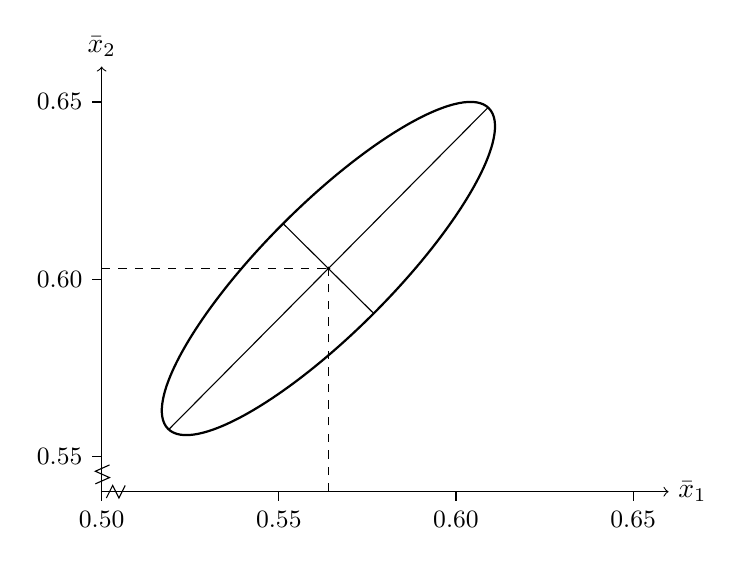
\begin{tikzpicture}[scale=1]
  \draw[->] (0,0) -- (7.2,0) node[right] {$\bar{x}_1$};
  \draw[->] (0,0) -- (0,5.4) node[above] {$\bar{x}_2$};
  \foreach \v/\p in {0.50/0,0.55/2.25,0.60/4.5,0.65/6.75}
    \draw (\p,0) -- (\p,-0.12) node[below] {\small $\v$};
  \foreach \v/\p in {0.55/0.45,0.60/2.70,0.65/4.95}
    \draw (0,\p) -- (-0.12,\p) node[left] {\small $\v$};
  % 坐标轴断裂记号
  \draw (0.30,0.08) -- (0.22,-0.08) -- (0.14,0.08) -- (0.06,-0.08);
  \draw (0.10,0.34) -- (-0.08,0.26) -- (0.10,0.18) -- (-0.08,0.10);
  % 中心虚线
  \draw[dashed] (2.88,0) -- (2.88,2.835);
  \draw[dashed] (0,2.835) -- (2.88,2.835);
  % 主、次轴
  \draw[thin] (0.852,0.790) -- (4.908,4.880);
  \draw[thin] (2.305,3.405) -- (3.455,2.265);
  % 置信椭圆
  \draw[thick,rotate around={45:(2.88,2.835)}] (2.88,2.835) ellipse (2.88cm and 0.81cm);
  \fill (2.88,2.835) circle (0.7pt);
\end{tikzpicture}
\phantomsection\label{fig:5.1}\mvcap{图 5.1\quad 微波炉辐射数据 $\boldsymbol{\mu}$ 的 95\% 置信椭圆}
\end{mvfigure}

%% ===== pg-183 =====

% ---- pg-183 ----
\[
\frac{2\sqrt{\hat{\lambda}_{1}}\sqrt{\frac{p(n-1)}{n(n-p)}F_{p,n-p}(\alpha)}}{2\sqrt{\hat{\lambda}_{2}}\sqrt{\frac{p(n-1)}{n(n-p)}F_{p,n-p}(\alpha)}}=\sqrt{\frac{\hat{\lambda}_{1}}{\hat{\lambda}_{2}}}=\frac{0.161}{0.045}=3.6
\]

即长轴的长度为短轴的 3.6 倍.\hfill$\blacksquare$

\mvsub{联合置信表示}

在置信域 $n(\bar{\mathbf{x}}-\boldsymbol{\mu})'\mathbf{S}^{-1}(\bar{\mathbf{x}}-\boldsymbol{\mu})\le c^{2}$ ($c$ 为常数) 给出有关 $\boldsymbol{\mu}$ 的似真值的联合信息的正确评估的同时, 其结论往往已包含了单个均值分量的置信表示. 在此过程中, 我们承认了下列看法, 即所有的各置信表示形式均应以一特定的概率同时成立. 我们引入所谓的联合置信区间, 就是为了保证以一特定的概率避免任一置信表示发生错误. 我们通过考虑与基于 $T^{2}$ 统计量的联合置信域密切相关的联合置信表示来开始我们的讨论.

设 $\mathbf{X}$ 服从 $N_{p}(\boldsymbol{\mu},\boldsymbol{\Sigma})$ 分布, 考虑线性组合
\[
Z=a_{1}X_{1}+a_{2}X_{2}+\cdots+a_{p}X_{p}=\mathbf{a}'\mathbf{X}
\]

由\hyperref[eq:2-43]{式(2-43)}知
\[
\mu_{Z}=E(Z)=\mathbf{a}'\boldsymbol{\mu}, \qquad \sigma_{Z}^{2}=\operatorname{Var}(Z)=\mathbf{a}'\boldsymbol{\Sigma}\mathbf{a}
\]

因此, 由结论 4.2 知, $Z$ 服从 $N(\mathbf{a}'\boldsymbol{\mu},\mathbf{a}'\boldsymbol{\Sigma}\mathbf{a})$ 分布. 如果 $\mathbf{X}_{1},\mathbf{X}_{2},\cdots,\mathbf{X}_{n}$ 为来自总体 $N_{p}(\boldsymbol{\mu},\boldsymbol{\Sigma})$ 的一随机样本, 则相应的 $Z$ 的样本可通过取线性组合产生. 因此,
\[
Z_{j}=a_{1}X_{j1}+a_{2}X_{j2}+\cdots+a_{p}X_{jp}=\mathbf{a}'\mathbf{X}_{j}, \qquad j=1,2,\cdots,n
\]

由\hyperref[eq:3-36]{式(3-36)}, 观察值 $z_{1},z_{2},\cdots,z_{n}$ 的样本均值和样本方差分别为
\[
\bar{z}=\mathbf{a}'\bar{\mathbf{x}} \ \text{ 和 }\ s_{z}^{2}=\mathbf{a}'\mathbf{S}\mathbf{a}
\]

这里 $\bar{\mathbf{x}}$ 和 $\mathbf{S}$ 分别为 $\mathbf{X}_{j}$ 的样本均值向量和协方差矩阵.

通过对各种不同的 $\mathbf{a}$ 考虑 $\mathbf{a}'\boldsymbol{\mu}$ 的置信区间, 便可得出所要的联合置信区间, 其过程如下:

当 $\mathbf{a}$ 固定且 $\sigma_{Z}^{2}$ 未知时, $\mu_{Z}=\mathbf{a}'\boldsymbol{\mu}$ 的 $100(1-\alpha)\%$ 置信区间根据 $t$ 统计量
\phantomsection\label{eq:5-20}
\begin{equation}
t=\frac{\bar{z}-\mu_{Z}}{s_{z}/\sqrt{n}}=\frac{\sqrt{n}(\mathbf{a}'\bar{\mathbf{x}}-\mathbf{a}'\boldsymbol{\mu})}{\sqrt{\mathbf{a}'\mathbf{S}\mathbf{a}}} \tag{5-20}
\end{equation}

得出, 故置信区间为
\[
\bar{z}-t_{n-1}(\alpha/2)\frac{s_{z}}{\sqrt{n}}\le \mu_{Z}\le \bar{z}+t_{n-1}(\alpha/2)\frac{s_{z}}{\sqrt{n}}
\]

即
\phantomsection\label{eq:5-21}
\begin{equation}
\mathbf{a}'\bar{\mathbf{x}}-t_{n-1}(\alpha/2)\sqrt{\frac{\mathbf{a}'\mathbf{S}\mathbf{a}}{n}}\le \mathbf{a}'\boldsymbol{\mu}\le \mathbf{a}'\bar{\mathbf{x}}+t_{n-1}(\alpha/2)\sqrt{\frac{\mathbf{a}'\mathbf{S}\mathbf{a}}{n}} \tag{5-21}
\end{equation}

其中 $t_{n-1}(\alpha/2)$ 为自由度为 $n-1$ 的 $t$ 分布的 $100(\alpha/2)$ 百分位数.

不等\hyperref[eq:5-21]{式(5-21)}可以理解成均值向量 $\boldsymbol{\mu}$ 的分量的置信表示形式, 例如对 $\mathbf{a}'=[1,0,\cdots,0]$, $\mathbf{a}'\boldsymbol{\mu}=\mu_{1}$, 因而\hyperref[eq:5-21]{式(5-21)}就是某个正态总体均值通常的置信区间(注意, 此时 $\mathbf{a}'\mathbf{S}\mathbf{a}=s_{11}$). 显然, 通过选择不同的系数向量 $\mathbf{a}$, 便可得到 $\boldsymbol{\mu}$ 的分量的若干个置信系数均为 $1-\alpha$ 的置信区间, 但此时的置信度就不再是 $1-\alpha$ 了.

直观地看, 我们总期望把由所有 $\mathbf{a}$ 的选择所生成的置信区间同某个“总”置信系数 $1-\alpha$ 联系在一起, 不过代价是要放弃大的联合置信系数的便利性, 即对一特定的 $\mathbf{a}$, 它们的区间长度要比\hyperref[eq:5-21]{式(5-21)}的大.

给定一个数据集 $\mathbf{x}_{1},\mathbf{x}_{2},\cdots,\mathbf{x}_{n}$ 和特定的 $\mathbf{a}$, \hyperref[eq:5-21]{式(5-21)}的置信区间是满足

%% ===== pg-184 =====

% ---- pg-184 ----
\[
|t|=\left|\frac{\sqrt{n}(\mathbf{a}'\bar{\mathbf{x}}-\mathbf{a}'\boldsymbol{\mu})}{\sqrt{\mathbf{a}'\mathbf{S}\mathbf{a}}}\right|\le t_{n-1}(\alpha/2)
\]

的 $\mathbf{a}'\boldsymbol{\mu}$ 值的集合, 或者说是满足
\phantomsection\label{eq:5-22}
\begin{equation}
t^{2}=\frac{n(\mathbf{a}'\bar{\mathbf{x}}-\mathbf{a}'\boldsymbol{\mu})^{2}}{\mathbf{a}'\mathbf{S}\mathbf{a}}=\frac{n(\mathbf{a}'(\bar{\mathbf{x}}-\boldsymbol{\mu}))^{2}}{\mathbf{a}'\mathbf{S}\mathbf{a}}\le t_{n-1}^{2}(\alpha/2) \tag{5-22}
\end{equation}

的 $\mathbf{a}'\boldsymbol{\mu}$ 值的集合. 让 $\mathbf{a}$ 变化, 我们可以通过使 $t^{2}$ 相对较小的 $\mathbf{a}'\boldsymbol{\mu}$ 值的集合来确定联合置信域. 在通过对 $\mathbf{a}$ 的许多选择来得到相应的置信域表示时, 将\hyperref[eq:5-22]{式(5-22)}中的常数 $t_{n-1}^{2}(\alpha/2)$ 以较大的 $c^{2}$ 值代替似乎是合理的.

现考虑满足 $t^{2}\le c^{2}$ 的 $\mathbf{a}$ 值, 我们的目标自然是要求最大值
\[
\max_{\mathbf{a}} t^{2}=\max_{\mathbf{a}}\frac{n(\mathbf{a}'(\bar{\mathbf{x}}-\boldsymbol{\mu}))^{2}}{\mathbf{a}'\mathbf{S}\mathbf{a}}
\]

在最大化引理(2-50)中, 令 $\mathbf{x}=\mathbf{a}, d=(\bar{\mathbf{x}}-\boldsymbol{\mu})$, 及 $\mathbf{B}=\mathbf{S}$, 就有
\phantomsection\label{eq:5-23}
\begin{equation}
\max_{\mathbf{a}}\frac{n(\mathbf{a}'(\bar{\mathbf{x}}-\boldsymbol{\mu}))^{2}}{\mathbf{a}'\mathbf{S}\mathbf{a}}=n\left[\max_{\mathbf{a}}\frac{(\mathbf{a}'(\bar{\mathbf{x}}-\boldsymbol{\mu}))^{2}}{\mathbf{a}'\mathbf{S}\mathbf{a}}\right]=n(\bar{\mathbf{x}}-\boldsymbol{\mu})'\mathbf{S}^{-1}(\bar{\mathbf{x}}-\boldsymbol{\mu})=T^{2} \tag{5-23}
\end{equation}

最大值在 $\mathbf{a}$ 与 $\mathbf{S}^{-1}(\bar{\mathbf{x}}-\boldsymbol{\mu})$ 成比例时达到.

\mvthm{结论 5.3}{设 $\mathbf{X}_{1},\mathbf{X}_{2},\cdots,\mathbf{X}_{n}$ 为来自总体 $N_{p}(\boldsymbol{\mu},\boldsymbol{\Sigma})$ 的随机样本, 且 $\boldsymbol{\Sigma}$ 为正定阵, 则对所有 $\mathbf{a}$, 区间
\[
\left(\mathbf{a}'\bar{\mathbf{X}}-\sqrt{\frac{p(n-1)}{n(n-p)}F_{p,n-p}(\alpha)\mathbf{a}'\mathbf{S}\mathbf{a}},\ \mathbf{a}'\bar{\mathbf{X}}+\sqrt{\frac{p(n-1)}{n(n-p)}F_{p,n-p}(\alpha)\mathbf{a}'\mathbf{S}\mathbf{a}}\right)
\]
以概率 $1-\alpha$ 包含 $\mathbf{a}'\boldsymbol{\mu}$.}

证明\quad 由\hyperref[eq:5-23]{式(5-23)}, $T^{2}=n(\bar{\mathbf{x}}-\boldsymbol{\mu})'\mathbf{S}^{-1}(\bar{\mathbf{x}}-\boldsymbol{\mu})\le c^{2}$ 意味着对所有 $\mathbf{a}$ 有 $\dfrac{n(\mathbf{a}'\bar{\mathbf{x}}-\mathbf{a}'\boldsymbol{\mu})^{2}}{\mathbf{a}'\mathbf{S}\mathbf{a}}\le c^{2}$, 即对所有 $\mathbf{a}$ 有
\[
\mathbf{a}'\bar{\mathbf{x}}-c\sqrt{\frac{\mathbf{a}'\mathbf{S}\mathbf{a}}{n}}\le \mathbf{a}'\boldsymbol{\mu}\le \mathbf{a}'\bar{\mathbf{x}}+c\sqrt{\frac{\mathbf{a}'\mathbf{S}\mathbf{a}}{n}}
\]

取 $c^{2}=p(n-1)F_{p,n-p}(\alpha)/(n-p)$ [见\hyperref[eq:5-6]{式(5-6)}], 故对所有 $\mathbf{a}$, 结论中的区间以概率 $1-\alpha=P[T^{2}\le c^{2}]$ 包含 $\mathbf{a}'\boldsymbol{\mu}$.\hfill$\blacksquare$

由于置信概率由 $T^{2}$ 分布确定, 因此为方便起见, 今后我们称结论 5.3 的联合置信区间为 $T^{2}$ 区间. 在 $T^{2}$ 区间中依次选取 $\mathbf{a}'=[1,0,\cdots,0], \mathbf{a}'=[0,1,\cdots,0], \cdots, \mathbf{a}'=[0,0,\cdots,1]$. 我们便得出下列诸式以置信系数 $1-\alpha$ 同时成立的结论:
\phantomsection\label{eq:5-24}
\begin{equation}
\begin{aligned}
\bar{x}_{1}-\sqrt{\frac{p(n-1)}{(n-p)}F_{p,n-p}(\alpha)}\sqrt{\frac{s_{11}}{n}}\ &\le\ \mu_{1}\ \le\ \bar{x}_{1}+\sqrt{\frac{p(n-1)}{(n-p)}F_{p,n-p}(\alpha)}\sqrt{\frac{s_{11}}{n}}\\
\bar{x}_{2}-\sqrt{\frac{p(n-1)}{(n-p)}F_{p,n-p}(\alpha)}\sqrt{\frac{s_{22}}{n}}\ &\le\ \mu_{2}\ \le\ \bar{x}_{2}+\sqrt{\frac{p(n-1)}{(n-p)}F_{p,n-p}(\alpha)}\sqrt{\frac{s_{22}}{n}}\\
&\qquad\qquad\qquad\vdots\qquad\qquad\qquad\qquad\vdots\\
\bar{x}_{p}-\sqrt{\frac{p(n-1)}{(n-p)}F_{p,n-p}(\alpha)}\sqrt{\frac{s_{pp}}{n}}\ &\le\ \mu_{p}\ \le\ \bar{x}_{p}+\sqrt{\frac{p(n-1)}{(n-p)}F_{p,n-p}(\alpha)}\sqrt{\frac{s_{pp}}{n}}
\end{aligned} \tag{5-24}
\end{equation}

注意, 若取 $\mathbf{a}'=[0,\cdots,0,a_{i},0,\cdots,0,a_{k},0,\cdots,0]$, $a_{i}=1$ 且 $a_{k}=-1$, 则可得到差值 $\mu_{i}-\mu_{k}$ 的置信系数为 $1-\alpha$ 的置信区间, 此时 $\mathbf{a}'\mathbf{S}\mathbf{a}=s_{ii}-2s_{ik}+s_{kk}$, 故其置信区间为
\[
\bar{x}_{i}-\bar{x}_{k}-\sqrt{\frac{p(n-1)}{(n-p)}F_{p,n-p}(\alpha)}\sqrt{\frac{s_{ii}-2s_{ik}+s_{kk}}{n}}\le \mu_{i}-\mu_{k}
\]

%% ===== pg-185 =====

% ---- pg-185 ----
\phantomsection\label{eq:5-25}
\begin{equation}
\le \bar{x}_{i}-\bar{x}_{k}+\sqrt{\frac{p(n-1)}{(n-p)}F_{p,n-p}(\alpha)}\sqrt{\frac{s_{ii}-2s_{ik}+s_{kk}}{n}} \tag{5-25}
\end{equation}

联合 $T^{2}$ 置信区间的方法对数据探测是较理想的. 由于其置信系数 $1-\alpha$ 对任意的 $\mathbf{a}$ 保持不变, 因此, 根据数据实验应受到检验的诸分量 $\boldsymbol{\mu}$ 的线性组合可以被估计出来.

另外, 根据补充 5A 中的结论, 我们可以得到 $(\mu_{i},\mu_{k})$ 的置信域, 其中 $(\mu_{i},\mu_{k})$ 在以样本均值为中心的椭圆内, 即
\phantomsection\label{eq:5-26}
\begin{equation}
n\left[\bar{x}_{i}-\mu_{i}, \bar{x}_{k}-\mu_{k}\right]\begin{bmatrix}s_{ii}&s_{ik}\\s_{ik}&s_{kk}\end{bmatrix}^{-1}\begin{bmatrix}\bar{x}_{i}-\mu_{i}\\\bar{x}_{k}-\mu_{k}\end{bmatrix}\le \frac{p(n-1)}{n-p}F_{p,n-p}(\alpha) \tag{5-26}
\end{equation}

而它们所有的置信系数仍保持为 $1-\alpha$.

均值向量的单一分量的联合 $T^{2}$ 置信区间恰好为置信椭球在该分量轴上的投影. 我们在下一个例子中将说明置信椭球的投影与由\hyperref[eq:5-24]{式(5-24)}给出的联合置信区间之间的这种联系.

\noindent\textbf{例 5.4}\quad (联合置信区间作为置信椭球的投影)

在例 5.3 中, 我们得到了炉门关闭及开启时微波炉辐射测量值四次根的均值的 95\% 置信椭圆. 由\hyperref[eq:5-24]{式(5-24)}知, 这两个均值分量的 95\% 联合 $T^{2}$ 置信区间为
\[
\left(\bar{x}_{1}-\sqrt{\frac{p(n-1)}{(n-p)}F_{p,n-p}(0.05)}\sqrt{\frac{s_{11}}{n}}, \bar{x}_{1}+\sqrt{\frac{p(n-1)}{(n-p)}F_{p,n-p}(0.05)}\sqrt{\frac{s_{11}}{n}}\right)
\]
\[
=\left(0.564-\sqrt{\frac{2\times41}{40}\times3.23}\times\sqrt{\frac{0.014\,4}{42}}, 0.564+\sqrt{\frac{2\times41}{40}\times3.23}\times\sqrt{\frac{0.014\,4}{42}}\right)
\]
\[
=(0.516,0.612)
\]

\[
\left(\bar{x}_{2}-\sqrt{\frac{p(n-1)}{(n-p)}F_{p,n-p}(0.05)}\sqrt{\frac{s_{22}}{n}}, \bar{x}_{2}+\sqrt{\frac{p(n-1)}{(n-p)}F_{p,n-p}(0.05)}\sqrt{\frac{s_{22}}{n}}\right)
\]
\[
=\left(0.603-\sqrt{\frac{2\times41}{40}\times3.23}\times\sqrt{\frac{0.014\,6}{42}}, 0.603+\sqrt{\frac{2\times41}{40}\times3.23}\times\sqrt{\frac{0.014\,6}{42}}\right)
\]
\[
=(0.555,0.651)
\]

在\hyperref[fig:5.2]{图 5.2} 中, 我们重绘了例 5.3 中的 95\% 置信椭圆, 可以看出, 其 95\% 联合置信区间为此椭圆在其均值分量轴上的投影.

\begin{mvfigure}
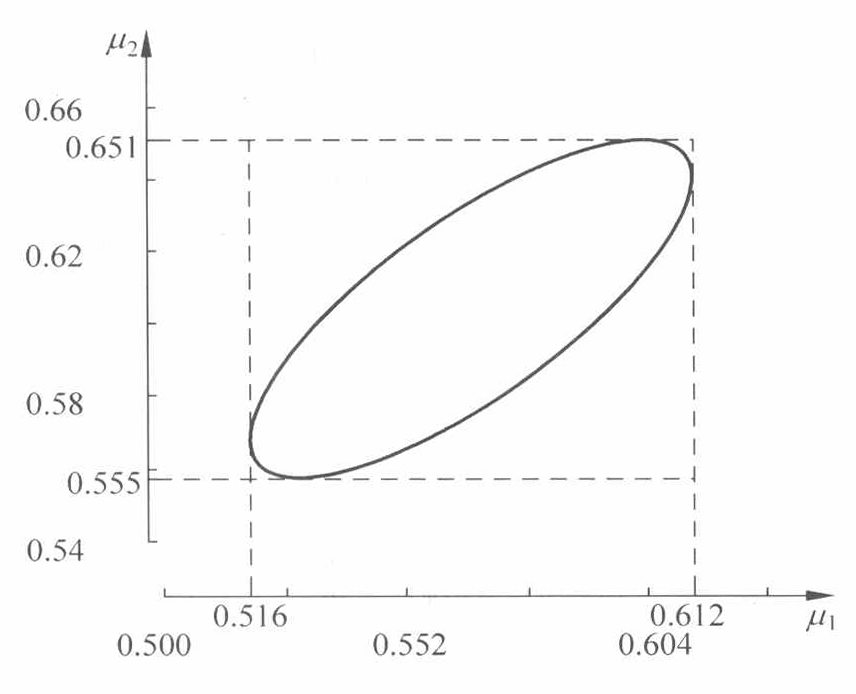
\includegraphics[width=72.5mm]{figs/fig_pg185_1.png}
\phantomsection\label{fig:5.2}\mvcap{图 5.2\quad 均值分量的联合 $T^{2}$ 区间作为置信椭圆在其轴上的投影——微波炉辐射数据}
\end{mvfigure}
\hfill$\blacksquare$

%% ===== pg-186 =====

% ---- pg-186 ----
\noindent\textbf{例 5.5}\quad (构造联合置信区间与置信椭圆)

\hyperref[tab:5.2]{表 5.2} 为 $n=87$ 名大学生参加大学水平考试计划课程 $X_{1}$ 及大学资格考试课程 $X_{2}$ 与 $X_{3}$ 的成绩.

\begin{mvtable}
\phantomsection\label{tab:5.2}\mvtabcap{表 5.2\quad 大学考试数据}
\footnotesize
\setlength{\tabcolsep}{4pt}
\begin{longtable}{rrrrrrrr}\toprule
考生 & $X_{1}$(社会科学与历史) & $X_{2}$(语言表达) & $X_{3}$(自然科学) & 考生 & $X_{1}$(社会科学与历史) & $X_{2}$(语言表达) & $X_{3}$(自然科学)\\
\midrule
\endfirsthead
\multicolumn{8}{c}{\zihao{6}续表}\\
\toprule
考生 & $X_{1}$(社会科学与历史) & $X_{2}$(语言表达) & $X_{3}$(自然科学) & 考生 & $X_{1}$(社会科学与历史) & $X_{2}$(语言表达) & $X_{3}$(自然科学)\\
\midrule
\endhead
\bottomrule
\endlastfoot

1 & 468 & 41 & 26 & 45 & 494 & 41 & 24\\
2 & 428 & 39 & 26 & 46 & 541 & 47 & 25\\
3 & 514 & 53 & 21 & 47 & 362 & 36 & 17\\
4 & 547 & 67 & 33 & 48 & 408 & 28 & 17\\
5 & 614 & 61 & 27 & 49 & 594 & 68 & 23\\
6 & 501 & 67 & 29 & 50 & 501 & 25 & 26\\
7 & 421 & 46 & 22 & 51 & 687 & 75 & 33\\
8 & 527 & 50 & 23 & 52 & 633 & 52 & 31\\
9 & 527 & 55 & 19 & 53 & 647 & 67 & 29\\
10 & 620 & 72 & 32 & 54 & 647 & 65 & 34\\
11 & 587 & 63 & 31 & 55 & 614 & 59 & 25\\
12 & 541 & 59 & 19 & 56 & 633 & 65 & 28\\
13 & 561 & 53 & 26 & 57 & 448 & 55 & 24\\
14 & 468 & 62 & 20 & 58 & 408 & 51 & 19\\
15 & 614 & 65 & 28 & 59 & 441 & 35 & 22\\
16 & 527 & 48 & 21 & 60 & 435 & 60 & 20\\
17 & 507 & 32 & 27 & 61 & 501 & 54 & 21\\
18 & 580 & 64 & 21 & 62 & 507 & 42 & 24\\
19 & 507 & 59 & 21 & 63 & 620 & 71 & 36\\
20 & 521 & 54 & 23 & 64 & 415 & 52 & 20\\
21 & 574 & 52 & 25 & 65 & 554 & 69 & 30\\
22 & 587 & 64 & 31 & 66 & 348 & 28 & 18\\
23 & 488 & 51 & 27 & 67 & 468 & 49 & 25\\
24 & 488 & 62 & 18 & 68 & 507 & 54 & 26\\
25 & 587 & 56 & 26 & 69 & 527 & 47 & 31\\
26 & 421 & 38 & 16 & 70 & 527 & 47 & 26\\
27 & 481 & 52 & 26 & 71 & 435 & 50 & 28\\
28 & 428 & 40 & 19 & 72 & 660 & 70 & 25\\
29 & 640 & 65 & 25 & 73 & 733 & 73 & 33\\
30 & 574 & 61 & 28 & 74 & 507 & 45 & 28\\
31 & 547 & 64 & 27 & 75 & 527 & 62 & 29\\
32 & 580 & 64 & 28 & 76 & 428 & 37 & 19\\
33 & 494 & 53 & 26 & 77 & 481 & 48 & 23\\
34 & 554 & 51 & 21 & 78 & 507 & 61 & 19\\
35 & 647 & 58 & 23 & 79 & 527 & 66 & 23\\
36 & 507 & 65 & 23 & 80 & 488 & 41 & 28\\
37 & 454 & 52 & 28 & 81 & 607 & 69 & 28\\
38 & 427 & 57 & 21 & 82 & 561 & 59 & 34\\
39 & 521 & 66 & 26 & 83 & 614 & 70 & 23\\
40 & 468 & 57 & 14 & 84 & 527 & 49 & 30\\
41 & 587 & 55 & 30 & 85 & 474 & 41 & 16\\
42 & 507 & 61 & 31 & 86 & 441 & 47 & 26\\
43 & 574 & 54 & 31 & 87 & 607 & 67 & 32\\
44 & 507 & 53 & 23 & & & & \\
\end{longtable}

资料来源：数据经 Richard W. Johnson 许可使用.
\end{mvtable}

%% ===== pg-187 =====

% ---- pg-187 ----
表中的 $X_{1},X_{2},X_{3}$ 分别代表社会科学与历史、语言表达及自然科学三门课程的考试成绩. 由表中的数据可得
\[
\bar{\mathbf{x}}=\begin{bmatrix}526.29\\54.69\\25.13\end{bmatrix}, \quad \mathbf{S}=\begin{bmatrix}5\,808.06&597.84&222.03\\597.84&126.05&23.39\\222.03&23.39&23.11\end{bmatrix}
\]

现计算 $\mu_{1},\mu_{2},\mu_{3}$ 的 95\% 联合置信区间. 由于
\[
\frac{p(n-1)}{n-p}F_{p,n-p}(\alpha)=\frac{3\times(87-1)}{(87-3)}F_{3,84}(0.05)=\frac{3\times86}{84}\times2.7=8.29
\]

可以得到联合置信区间[见\hyperref[eq:5-24]{式(5-24)}]为
\[
526.29-\sqrt{8.29}\times\sqrt{\frac{5\,808.06}{87}}\le \mu_{1}\le 526.29+\sqrt{8.29}\times\sqrt{\frac{5\,808.06}{87}}
\]

即
\[
503.06\le \mu_{1}\le 550.12
\]

\[
54.69-\sqrt{8.29}\times\sqrt{\frac{126.05}{87}}\le \mu_{2}\le 54.69+\sqrt{8.29}\times\sqrt{\frac{126.05}{87}}
\]

即
\[
51.22\le \mu_{2}\le 58.16
\]

\[
25.13-\sqrt{8.29}\times\sqrt{\frac{23.11}{87}}\le \mu_{3}\le 25.13+\sqrt{8.29}\times\sqrt{\frac{23.11}{87}}
\]

即
\[
23.65\le \mu_{3}\le 26.61
\]

除语言表达成绩外, 其边缘 $Q$-$Q$ 图及二维散点图表明, 并无迹象表明有严重背离大学资格考试数据的正态性的现象产生(见练习 5.18). 此外, 即使数据不是严格服从正态分布, 这么大的样本容量也足以保证该方法的合理性(见 5.5 节).

由于上述三个置信区间均必须以 95\% 的置信度成立, 因此其联合 $T^{2}$ 区间要比一元置信区间更宽些. 又因为可以用同样的置信度来构造它们之间差值的置信区间, 所以这些置信区间也许比通常所需的更宽.

例如, 对 $\mathbf{a}'=[0,1,-1]$, $\mu_{2}-\mu_{3}$ 的置信区间的两个端点为
\[
(\bar{x}_{2}-\bar{x}_{3})\pm\sqrt{\frac{p(n-1)}{(n-p)}F_{p,n-p}(0.05)}\sqrt{\frac{s_{22}+s_{33}-2s_{23}}{n}}
\]
\[
=(54.69-25.13)\pm\sqrt{8.29}\times\sqrt{\frac{126.05+23.11-2\times23.39}{87}}
\]
\[
=29.56\pm3.12
\]

故 $\mu_{2}-\mu_{3}$ 的 95\% 置信区间为 $(26.44,32.68)$. 对其他差值同样可构造其联合置信区间.

最后, 能以相同的 95\% 置信度构造每对均值的置信椭圆. 比如, 对 $(\mu_{2},\mu_{3})$ 这对均值来说, 有
\[
87\times[54.69-\mu_{2}, 25.13-\mu_{3}]\begin{bmatrix}126.05&23.39\\23.39&23.11\end{bmatrix}^{-1}\begin{bmatrix}54.69-\mu_{2}\\25.13-\mu_{3}\end{bmatrix}
\]
\[
=0.849\times(54.69-\mu_{2})^{2}+4.633\times(25.13-\mu_{3})^{2}
\]
\[
\qquad -2\times0.859\times(54.69-\mu_{2})\times(25.13-\mu_{3})\le 8.29
\]

该椭圆及另外两对均值的 95\% 置信椭圆的图形见\hyperref[fig:5.3]{图 5.3}. 图中还给出了这些椭圆在其均值分量轴上的投影, 这些投影即为 $T^{2}$ 区间.

%% ===== pg-188 =====

% ---- pg-188 ----
\begin{mvfigure}
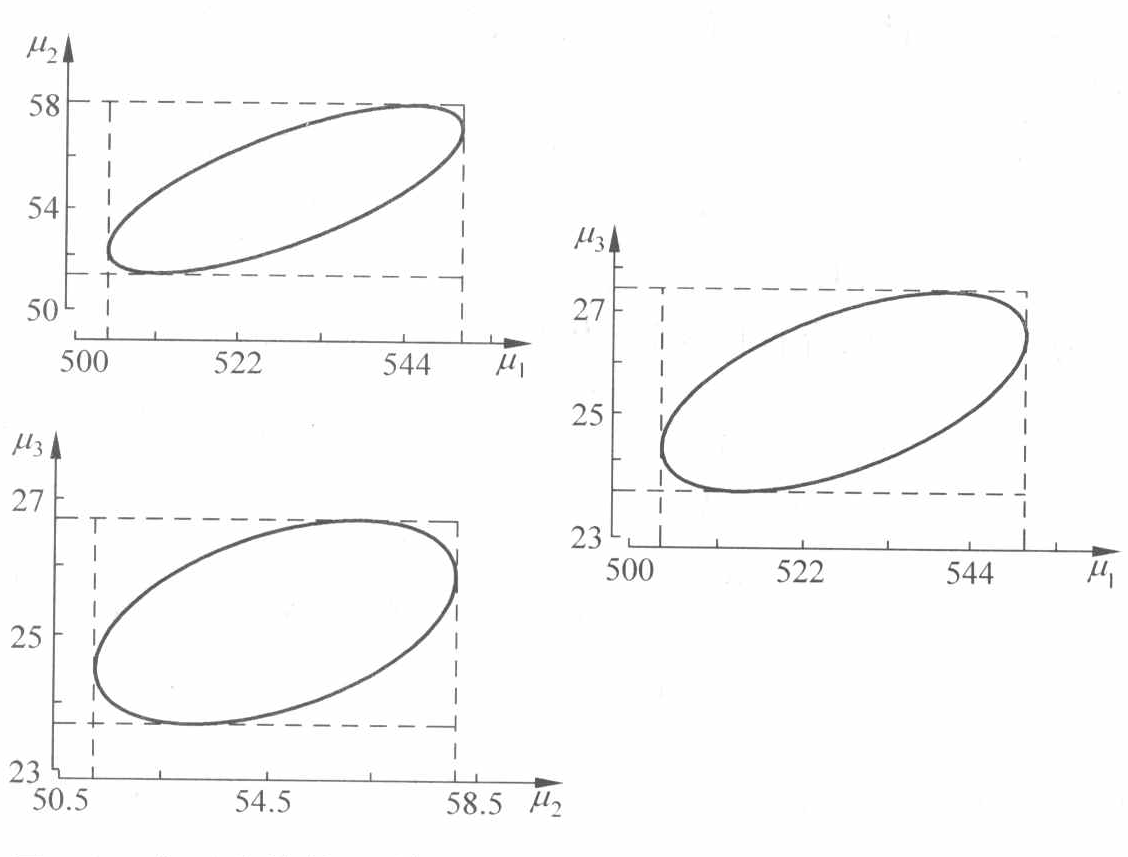
\includegraphics[width=95.5mm]{figs/fig_pg188_1.png}
\phantomsection\label{fig:5.3}\mvcap{图 5.3\quad 各对均值的 95\% 置信椭圆及联合 $T^{2}$ 区间——大学考试数据}
\end{mvfigure}
\hfill$\blacksquare$

\mvsub{联合置信区间与单一置信区间的比较}

构造置信区间的另一种方法是每次只考虑一个分量 $\mu_{i}$, 正如当 $\mathbf{a}'=[0,\cdots,0,a_{i},0,\cdots,0]$ (此处 $a_{i}=1$) 时\hyperref[eq:5-21]{式(5-21)}所暗示的那样. 这种方法不必考虑 $p$ 维变量的协方差矩阵的结构, 就可得到置信区间
\phantomsection\label{eq:5-27}
\begin{equation}
\begin{aligned}
\bar{x}_{1}-t_{n-1}\left(\frac{\alpha}{2}\right)\sqrt{\frac{s_{11}}{n}}\ &\le\ \mu_{1}\ \le\ \bar{x}_{1}+t_{n-1}\left(\frac{\alpha}{2}\right)\sqrt{\frac{s_{11}}{n}}\\
\bar{x}_{2}-t_{n-1}\left(\frac{\alpha}{2}\right)\sqrt{\frac{s_{22}}{n}}\ &\le\ \mu_{2}\ \le\ \bar{x}_{2}+t_{n-1}\left(\frac{\alpha}{2}\right)\sqrt{\frac{s_{22}}{n}}\\
&\qquad\qquad\vdots\qquad\qquad\qquad\vdots\\
\bar{x}_{p}-t_{n-1}\left(\frac{\alpha}{2}\right)\sqrt{\frac{s_{pp}}{n}}\ &\le\ \mu_{p}\ \le\ \bar{x}_{p}+t_{n-1}\left(\frac{\alpha}{2}\right)\sqrt{\frac{s_{pp}}{n}}
\end{aligned} \tag{5-27}
\end{equation}

虽然在抽样之前第 $i$ 个区间包含 $\mu_{i}$ 的概率为 $1-\alpha$, 但一般而言, 对其他区间包含各自的 $\mu_{i}$ 的概率并不能断言什么. 正如我们在前面指出的, 这个概率并非 $1-\alpha$.

为了更清楚地说明这个问题, 考虑观测值服从正态分布且
\[
\boldsymbol{\Sigma}=\begin{bmatrix}\sigma_{11}&0&\cdots&0\\0&\sigma_{22}&\cdots&0\\\vdots&\vdots&\ddots&\vdots\\0&0&\cdots&\sigma_{pp}\end{bmatrix}
\]
的特殊情形. 由于第一个变量的观测值与第二个变量的观测值相互独立, 故可应用独立事件的乘法法则, 因而在样本被抽取之前有
\[
\begin{aligned}
P[\text{式(5-27) 中的所有 }t\text{ 区间包含各自的 }\mu_{i}]&=(1-\alpha)(1-\alpha)\cdots(1-\alpha)\\
&=(1-\alpha)^{p}
\end{aligned}
\]

若 $1-\alpha=0.95$ 且 $p=6$, 则此概率为 $0.95^{6}=0.74$.

为保证所有均值分量的置信表示同时成立的概率为 $1-\alpha$, 其各自的置信区间要比其 $t$ 区

%% ===== pg-189 =====

% ---- pg-189 ----
间大, 至于多大, 这就与 $p,n$ 及 $1-\alpha$ 三者的大小有关.

对 $1-\alpha=0.95, n=15$ 和 $p=4$, \hyperref[eq:5-24]{式(5-24)}及\hyperref[eq:5-27]{式(5-27)}中 $\sqrt{s_{ii}/n}$ 前的系数分别为
\[
\sqrt{\frac{p(n-1)}{(n-p)}F_{p,n-p}(0.05)}=\sqrt{\frac{4\times14}{11}}\times3.36=4.14
\]
及 $t_{n-1}(0.025)=2.145$. 因此这种情况下的联合置信区间要比单一 $t$ 区间宽 $100\times(4.14-2.145)/2.145=93\%$.

\hyperref[tab:5.3]{表 5.3} 给出了按\hyperref[eq:5-21]{式(5-21)}算出的单一 $t$ 区间及相应的联合 $T^{2}$ 区间的距离乘数的临界值. 一般来说, 相对 $t$ 区间而言, $T^{2}$ 区间的宽度当 $n$ 固定而 $p$ 增大时增大; 当 $p$ 固定而 $n$ 增大时减小.

\begin{mvtable}
\phantomsection\label{tab:5.3}\mvtabcap{表 5.3\quad 对选定的 $n$ 与 $p$ ($1-\alpha=0.95$) 单一 $t$ 区间与 $T^{2}$ 区间的距离乘数之临界值}
\begin{tabular}{rccc}
\toprule
\multirow{2}{*}{$n$} & \multirow{2}{*}{$t_{n-1}(0.025)$} & \multicolumn{2}{c}{$\sqrt{\dfrac{(n-1)p}{(n-p)}F_{p,n-p}(0.05)}$}\\
\cmidrule(lr){3-4}
& & $p=4$ & $p=10$\\
\midrule
15 & 2.145 & 4.14 & 11.52\\
25 & 2.064 & 3.60 & 6.39\\
50 & 2.010 & 3.31 & 5.05\\
100 & 1.970 & 3.19 & 4.61\\
$\infty$ & 1.960 & 3.08 & 4.28\\
\bottomrule
\end{tabular}
\end{mvtable}

将\hyperref[tab:5.3]{表 5.3} 中的置信区间进行比较显然有些不公平, 因为对固定的 $n$ 与 $p$, 其所有的 $T^{2}$ 区间相联系的置信水平为 0.95, 而在同样的 $n$ 值, 所有单一 $t$ 区间的置信水平却比 0.95 要小些. 单一 $t$ 区间的宽度太短, 以至于对所有 $p$ 个均值的单独置信区间不能有一个总的置信水平. 然而, 当这是唯一可作的推断时, 我们有时就把它们看作是均值的最佳可能信息. 此外, 如果仅当 $T^{2}$ 检验拒绝零假设时才计算单一置信区间, 那么有些研究者认为, 单一置信区间也许比 $T^{2}$ 区间更精确地代表有关均值的信息.

如果 $T^{2}$ 区间仅应用于 $p$ 个均值分量, 那么 $T^{2}$ 区间显然太宽. 为了说明其原因, 我们来考虑\hyperref[fig:5.2]{图 5.2} 中的置信椭圆及联合置信区间. 若 $\mu_{1},\mu_{2}$ 分别落在各自的 $T^{2}$ 区间内, 那么 $(\mu_{1},\mu_{2})$ 就落在由此两区间围成的矩形内. 此矩形显然包含了置信椭圆, 虽然置信椭圆更小些, 但它却以 0.95 的概率包含了均值向量 $\boldsymbol{\mu}=(\mu_{1},\mu_{2})$. 因此, 对由 $T^{2}$ 区间所围成的矩形而言, 其包含两个均值分量 $\mu_{1}$ 与 $\mu_{2}$ 的概率要大于 0.95. 这一结果促使我们去考虑第二种进行多重比较的方法, 即所谓的庞弗罗尼方法.

\mvsub{多重比较的庞弗罗尼方法}

人们常把注意力集中在少数的单一置信区间上, 在这些情形中, 可能会得到比结论 5.3 的联合置信区间更好的结论. 但如果均值分量 $\mu_{i}$ 的个数 $m$ 很小, 或者其线性组合 $\mathbf{a}_{i}'\boldsymbol{\mu}=a_{i1}\mu_{1}+a_{i2}\mu_{2}+\cdots+a_{ip}\mu_{p}$ 很小, 则可采用比联合 $T^{2}$ 区间更为精确的联合置信区间的方法. 另一种多重比较法就是庞弗罗尼方法, 它是由庞弗罗尼概率不等式引申而来的.

假设在得到数据之前, 已知 $m$ 个线性组合 $\mathbf{a}_{1}'\boldsymbol{\mu},\mathbf{a}_{2}'\boldsymbol{\mu},\cdots,\mathbf{a}_{m}'\boldsymbol{\mu}$ 的置信区间, 记 $C_{i}$ 为 $\mathbf{a}_{i}'\boldsymbol{\mu}$ 的置信表示, 满足 $P(C_{i}\text{ 为真})=1-\alpha_{i}, i=1,2,\cdots,m$, 我们有(见练习 5.6)
\[
P(\text{所有 }C_{i}\text{ 为真})=1-P(\text{至少有一个 }C_{i}\text{ 为假})
\]

%% ===== pg-190 =====

% ---- pg-190 ----
\phantomsection\label{eq:5-28}
\begin{equation}
\begin{aligned}
&\ge 1-\sum_{i=1}^{m}P(C_{i}\text{ 为假})=1-\sum_{i=1}^{m}(1-P(C_{i}\text{ 为真}))\\
&=1-(\alpha_{1}+\alpha_{2}+\cdots+\alpha_{m})
\end{aligned} \tag{5-28}
\end{equation}

不等\hyperref[eq:5-28]{式(5-28)}为庞弗罗尼不等式的一个特殊情形. 利用它, 研究人员总可控制总体误差率 $\alpha_{1}+\alpha_{2}+\cdots+\alpha_{m}$, 不管置信表示中隐藏着何种相关结构. 同时, 在控制一组重要置信表示的误差率以及使它与另一些不太重要的置信表示达成均衡中, 此法也是较为灵活的.

让我们来给出由 $\boldsymbol{\mu}$ 的分量 $\mu_{i}$ 组成的约束集的联合区间估计. 由于对这些分量的相对重要性缺乏了解, 我们考虑单一的 $t$ 区间:
\[
\bar{x}_{i}\pm t_{n-1}\left(\frac{\alpha_{i}}{2}\right)\sqrt{\frac{s_{ii}}{n}}, \qquad i=1,2,\cdots,m
\]

这里 $\alpha_{i}=\alpha/m$. 由于
\[
P[\bar{X}_{i}\pm t_{n-1}(\alpha/2m)\sqrt{s_{ii}/n}\text{ 包含 }\mu_{i}]=1-\alpha/m, \quad i=1,2,\cdots,m
\]

由\hyperref[eq:5-28]{式(5-28)}知
\[
P\left[\bar{X}_{i}\pm t_{n-1}\left(\frac{\alpha}{2m}\right)\sqrt{\frac{s_{ii}}{n}}\text{ 包含 }\mu_{i}, \forall i\right]\ge 1-\underbrace{\left(\frac{\alpha}{m}+\frac{\alpha}{m}+\cdots+\frac{\alpha}{m}\right)}_{m\text{ 项}}
\]
\[
=1-\alpha
\]

因此, 以不小于 $1-\alpha$ 的总置信水平, 可得下列 $m=p$ 个置信表示
\phantomsection\label{eq:5-29}
\begin{equation}
\begin{aligned}
\bar{x}_{1}-t_{n-1}\left(\frac{\alpha}{2p}\right)\sqrt{\frac{s_{11}}{n}}\ &\le\ \mu_{1}\ \le\ \bar{x}_{1}+t_{n-1}\left(\frac{\alpha}{2p}\right)\sqrt{\frac{s_{11}}{n}}\\
\bar{x}_{2}-t_{n-1}\left(\frac{\alpha}{2p}\right)\sqrt{\frac{s_{22}}{n}}\ &\le\ \mu_{2}\ \le\ \bar{x}_{2}+t_{n-1}\left(\frac{\alpha}{2p}\right)\sqrt{\frac{s_{22}}{n}}\\
&\qquad\qquad\vdots\qquad\qquad\vdots\\
\bar{x}_{p}-t_{n-1}\left(\frac{\alpha}{2p}\right)\sqrt{\frac{s_{pp}}{n}}\ &\le\ \mu_{p}\ \le\ \bar{x}_{p}+t_{n-1}\left(\frac{\alpha}{2p}\right)\sqrt{\frac{s_{pp}}{n}}
\end{aligned} \tag{5-29}
\end{equation}

将\hyperref[eq:5-29]{式(5-29)}与\hyperref[eq:5-24]{式(5-24)}进行比较, 我们发现\hyperref[eq:5-29]{式(5-29)}中仅以百分位数 $t_{n-1}(\alpha/2p)$ 替代了\hyperref[eq:5-24]{式(5-24)}中的 $\sqrt{(n-1)pF_{p,n-p}(\alpha)/(n-p)}$, 区间保持相同结构.

\medskip
\noindent\textbf{例 5.6}\quad (庞弗罗尼联合置信区间的构造以及与 $T^{2}$ 区间的比较)

仍考虑例 5.3 及例 5.4 中的微波炉辐射数据. 我们将给出均值 $\mu_{1}$ 与 $\mu_{2}$ 的 95\% 庞弗罗尼联合置信区间, 这里 $\alpha_{i}=0.05/2, i=1,2$. 利用例 5.3 的结论, 注意到 $n=42$ 及 $t_{41}(0.05/(2\times2))=t_{41}(0.012\,5)=2.327$, 可知
\[
\bar{x}_{1}\pm t_{41}(0.012\,5)\sqrt{\frac{s_{11}}{n}}=0.564\pm2.327\times\sqrt{\frac{0.014\,4}{42}} \quad\text{即}\quad 0.521\le \mu_{1}\le 0.607
\]
\[
\bar{x}_{2}\pm t_{41}(0.012\,5)\sqrt{\frac{s_{22}}{n}}=0.603\pm2.327\times\sqrt{\frac{0.014\,6}{42}} \quad\text{即}\quad 0.560\le \mu_{2}\le 0.646
\]

\hyperref[fig:5.4]{图 5.4} 给出了 $\mu_{1},\mu_{2}$ 的 95\% 联合 $T^{2}$ 置信区间以及相应的 95\% 庞弗罗尼置信区间(对应\hyperref[fig:5.2]{图 5.2}). 对每一均值分量, 其庞弗罗尼置信区间均落在 $T^{2}$ 区间内. 因此, 由其庞弗罗尼置信区间所围成的矩形区域包含在由其 $T^{2}$ 区间所围成的矩形区域中. 如果我们仅对均值分量感兴趣, 那么, 庞弗罗尼区间估计比 $T^{2}$ 区间估计更精确. 另一方面, 当考虑被测变量之间的相关性时, $\boldsymbol{\mu}$ 的 95\% 置信域还能给出 $(\mu_{1},\mu_{2})$ 的似真值.

%% ===== pg-191 =====

\begin{mvfigure}
\centering
\begin{tikzpicture}[scale=0.60]
\draw[->] (-0.4,0)--(13.6,0) node[right,font=\small]{$\mu_{1}$};
\draw[->] (0,-0.4)--(0,13.2) node[above,font=\small]{$\mu_{2}$};
% x 刻度
\foreach \v/\l in {0/0.500,1.6/0.516,2.1/0.521,5.2/0.552,10.4/0.604,10.7/0.607,11.2/0.612}
  \draw (\v,0.15)--(\v,-0.15) node[below,font=\tiny]{\l};
% y 刻度
\foreach \v/\l in {0/0.54,1.5/0.555,2.0/0.560,4.0/0.58,8.0/0.62,10.0/0.640,10.6/0.646,11.1/0.651,12/0.66}
  \draw (0.15,\v)--(-0.15,\v) node[left,font=\tiny]{\l};
% T² 边界（点线）
\draw[dotted] (1.6,2.0) rectangle (10.7,11.1);
% 庞弗罗尼边界（虚线）
\draw[dashed] (2.1,1.5) rectangle (10.4,10.6);
% 置信椭圆
\begin{scope}[shift={(6.15,6.5)},rotate=33]
\draw[thick] (0,0) ellipse (4.55 and 3.25);
\end{scope}
% 图例
\draw[dotted] (11.6,8.4)--(12.2,8.4);
\node[right,font=\scriptsize] at (12.2,8.4){$T^{2}$};
\draw[dashed] (11.6,7.3)--(12.2,7.3);
\node[right,font=\scriptsize] at (12.2,7.3){庞弗罗尼};
\end{tikzpicture}
\phantomsection\label{fig:5.4}\mvcap{图 5.4\quad 均值分量的 $95\%$ $T^{2}$ 区间与 $95\%$ 庞弗罗尼置信区间——微波炉辐射数据}
\end{mvfigure}
\hfill$\blacksquare$

线性组合 $\mathbf{a}'\boldsymbol{\mu}$ 的庞弗罗尼区间与 $T^{2}$ 区间均有形式 (回忆结论 5.3)
\[
\mathbf{a}'\bar{\mathbf{X}}\pm\text{临界值}\cdot\sqrt{\frac{\mathbf{a}'\mathbf{S}\mathbf{a}}{n}}
\]
因此, 对 $a_{i}=a/m$, 有
\phantomsection\label{eq:5-30}
\begin{equation}
\frac{\text{庞弗罗尼区间宽度}}{T^{2}\ \text{区间宽度}}=\frac{t_{n-1}(a/2m)}{\sqrt{\dfrac{p(n-1)}{n-p}F_{p,n-p}(a)}}
\tag{5-30}
\end{equation}
这个比值与随机量 $\bar{\mathbf{X}}$ 与 $\mathbf{S}$ 无关. 正如我们前面指出的, 对特定的 $\mathbf{a}'\boldsymbol{\mu}$, 当 $m$ 小时, 庞弗罗尼区间总要窄些. \hyperref[tab:5.4]{表 5.4} 对某些 $n$ 与 $p$ 值列出了其宽度要窄多少.

\begin{mvtable}
\phantomsection\label{tab:5.4}\mvtabcap{表 5.4\quad (庞弗罗尼区间宽度)/($T^{2}$ 区间宽度)}
\centering
$1-a=0.95,a_{i}=0.05/m$\\[4pt]
\begin{tabular}{cccc}
\toprule
\multirow{2}{*}{$n$} & \multicolumn{3}{c}{$m=p$}\\
\cmidrule(lr){2-4}
 & $2$ & $4$ & $10$\\
\midrule
$15$  & $0.88$ & $0.69$ & $0.29$\\
$25$  & $0.90$ & $0.75$ & $0.48$\\
$50$  & $0.91$ & $0.78$ & $0.58$\\
$100$ & $0.91$ & $0.80$ & $0.62$\\
$\infty$ & $0.91$ & $0.81$ & $0.66$\\
\bottomrule
\end{tabular}
\end{mvtable}

当 $m=p$ 时, 由\hyperref[tab:5.4]{表 5.4} 可知, 庞弗罗尼方法得到的置信区间要更窄些. 正因此法容易应用且能给出推断所需的较窄置信区间, 今后我们将经常根据庞弗罗尼方法使用联合 $t$ 区间.

\section{总体均值向量的大样本推断}
\phantomsection\label{sec:5.5}

当样本容量很大时, 我们不需要总体的正态性假定就可以构造 $\boldsymbol{\mu}$ 的假设检验及置信域. 正如练习 5.15, 5.16 和 5.17 所指出的, 对大的 $n$, 即使总体分布是离散型分布, 我们也能够对总体均值作出推断. 事实上, 对正态性的严重偏离可通过大样本来克服. 此时, 假设检验与联合置信表示都近似地具有名义上的置信水平.

%% ===== pg-192 =====

大样本的优越性, 也许部分地被只使用汇总统计量 $\bar{\mathbf{x}}$ 与 $\mathbf{S}$ 而造成的样本信息损失所抵消. 另一方面, 由于 $(\bar{\mathbf{x}},\mathbf{S})$ 是正态总体的充分统计量 [见\hyperref[eq:4-21]{式(4-21)}], 因此总体的分布与多元正态分布越接近, 统计推断中样本信息的利用就越充分.

所有 $\boldsymbol{\mu}$ 的大样本推断都是建立在 $\chi^{2}$ 分布基础上的, 由\hyperref[eq:4-28]{式(4-28)}, 我们知道 $(\bar{\mathbf{X}}-\boldsymbol{\mu})'(n^{-1}\boldsymbol{\Sigma})^{-1}(\bar{\mathbf{X}}-\boldsymbol{\mu})=n(\bar{\mathbf{X}}-\boldsymbol{\mu})'\boldsymbol{\Sigma}^{-1}(\bar{\mathbf{X}}-\boldsymbol{\mu})$ 近似服从自由度为 $p$ 的 $\chi^{2}$ 分布. 因此
\phantomsection\label{eq:5-31}
\begin{equation}
P\bigl[n(\bar{\mathbf{X}}-\boldsymbol{\mu})'\mathbf{S}^{-1}(\bar{\mathbf{X}}-\boldsymbol{\mu})\le\chi_{p}^{2}(a)\bigr]\doteq 1-a
\tag{5-31}
\end{equation}
其中 $\chi_{p}^{2}(a)$ 是 $\chi_{p}^{2}$ 分布的上 $100a$ 百分位数.

由\hyperref[eq:5-31]{式(5-31)} 可立即推得大样本假设检验与联合置信域. 其过程概括在下面的结论 5.4 与结论 5.5 中.

\mvthm{结论 5.4}{设 $\mathbf{X}_{1},\mathbf{X}_{2},\cdots,\mathbf{X}_{n}$ 为来自均值为 $\boldsymbol{\mu}$, 协方差阵为正定阵 $\boldsymbol{\Sigma}$ 的总体的一个随机样本. 当 $n-p$ 很大时, 若观测值
\[
n(\bar{\mathbf{x}}-\boldsymbol{\mu}_{0})'\mathbf{S}^{-1}(\bar{\mathbf{x}}-\boldsymbol{\mu}_{0})>\chi_{p}^{2}(a)
\]
我们就在大约为 $a$ 的置信水平下拒绝 $H_{0}:\boldsymbol{\mu}=\boldsymbol{\mu}_{0}$ 而接受 $H_{1}:\boldsymbol{\mu}\ne\boldsymbol{\mu}_{0}$, 这里 $\chi_{p}^{2}(a)$ 是自由度为 $p$ 的上 $100a$ 百分位数.}
\hfill$\blacksquare$

将结论 5.4 中的检验与\hyperref[eq:5-7]{式(5-7)} 中相应的正态理论检验作比较, 我们发现它们的检验统计量具有相同的结构, 只是临界值有所不同. 但进一步的考察揭示: 当结论 5.4 的 $\chi^{2}$ 检验较为适宜时, 两种检验基本上给出相同的结果. 这主要是因为, 当 $n$ 相对于 $p$ 较大时, $(n-1)pF_{p,n-p}(a)/(n-p)$ 与 $\chi_{p}^{2}(a)$ 近似相等 (见附录中的表 3 和表 4).

\mvthm{结论 5.5}{设 $\mathbf{X}_{1},\mathbf{X}_{2},\cdots,\mathbf{X}_{n}$ 为来自均值为 $\boldsymbol{\mu}$, 协方差阵为正定阵 $\boldsymbol{\Sigma}$ 的总体的一个随机样本. 当 $n-p$ 很大时, 对所有的 $\mathbf{a}$, $\mathbf{a}'\bar{\mathbf{X}}\pm\sqrt{\chi_{p}^{2}(a)}\sqrt{\dfrac{\mathbf{a}'\mathbf{S}\mathbf{a}}{n}}$ 包含 $\mathbf{a}'\boldsymbol{\mu}$ 的概率近似为 $1-a$. 因此, 我们有 $100(1-a)\%$ 的联合置信表示}

\begin{center}
\begin{tabular}{ccccc}
$\bar{x}_{1}\pm\sqrt{\chi_{p}^{2}(a)}\sqrt{\dfrac{s_{11}}{n}}$ & 包含 & $\mu_{1}$ & &\\[10pt]
$\bar{x}_{2}\pm\sqrt{\chi_{p}^{2}(a)}\sqrt{\dfrac{s_{22}}{n}}$ & 包含 & $\mu_{2}$ & &\\[10pt]
$\vdots$ & & $\vdots$ & &\\[6pt]
$\bar{x}_{p}\pm\sqrt{\chi_{p}^{2}(a)}\sqrt{\dfrac{s_{pp}}{n}}$ & 包含 & $\mu_{p}$ & &
\end{tabular}
\end{center}

此外, 对所有 $(\mu_{i},\mu_{k}),i,k=1,2,\cdots,p$, 以样本均值为中心的置信椭圆
\[
n\bigl[\bar{x}_{i}-\mu_{i},\bar{x}_{k}-\mu_{k}\bigr]
\begin{bmatrix}s_{ii}&s_{ik}\\s_{ik}&s_{kk}\end{bmatrix}^{-1}
\begin{bmatrix}\bar{x}_{i}-\mu_{i}\\\bar{x}_{k}-\mu_{k}\end{bmatrix}\le\chi_{p}^{2}(a)
\]
包含 $(\mu_{i},\mu_{k})$ 的概率近似为 $1-a$.

\medskip
\noindent\mvbold{证明}\quad 第一部分的结论可从结论 5A.1 推出, 其中 $c^{2}=\chi_{p}^{2}(a)$. 概率水平由\hyperref[eq:5-31]{式(5-31)} 给出. 若取 $\mathbf{a}'=[0,\cdots,0,a_{i},0,\cdots,0],a_{i}=1,i=1,2,\cdots,p$, 就可得到 $\mu_{i}$ 的置信表示. 各对均值的置信椭圆的结论可从结论 5A.2 推出, 其中 $c^{2}=\chi_{p}^{2}(a)$. 所有置信表示的总置信水平均为 $1-a$ 这一结论, 同样是\hyperref[eq:5-31]{式(5-31)} 所归纳的大样本分布理论的结果.\hfill$\blacksquare$

很难说什么样的样本才算一个大的样本. 在一维或者二维的情况中, 样本容量在 30 至 50

%% ===== pg-193 =====

之间通常认为是一个大的样本. 随着数据特征的变大,为了得到不同的检验统计量的真实分布的良好的渐进逼近,我们需要更大的样本容量. 我们不打算论证地简单认为 $n-p$ 必须是大的,并且意识到真实情况会更加复杂. 对 $p=2$ 且样本容量为 50 的应用和 $p=52$ 且样本容量为 100 的应用是很不一样,尽管两种情况 $n-p$ 都等于 48.

对这些大样本推断方法进行正态理论所要求的各种检验,这是一种很好的统计实践. 虽然当 $n$ 很大时,对正态性的微小甚至中等程度的偏离一般不会引起任何问题,但过大的偏差就会产生问题,特别是真实误差率会远远地偏离其名义误差率水平 $\alpha$. 如果在 Q-Q 散点图和其他考察方法中发现存在离群值和其他过大的偏差(例如,参见[2]),则应采取适当的校正措施,包括对数据进行变换. 对称多元分布均值向量的检验方法相对来说,对偏离正态性不很敏感,这些方法在文献[11]中有所讨论. 在某些情形下,结论 5.4 和结论 5.5 仅对非常大的样本才有效.

下面的例子用来解释如何对单一均值向量构造大样本联合置信区间的问题.

\noindent\textbf{例 5.7}\quad (构造大样本联合置信区间)

一名音乐教育工作者为制定芬兰的音乐教育标准,测试了数千名芬兰学生的音乐才能,部分统计数据见\hyperref[tab:5.5]{表 5.5}. 这些统计数据来自自由 $n=96$ 名芬兰 12 年级学生组成的样本:

\begin{mvtable}
\phantomsection\label{tab:5.5}\mvtabcap{表 5.5\quad 96 名 12 年级芬兰学生音乐才能测试数据的均值与标准差}
\begin{tabular}{lcc}
\toprule
\multirow{2}{*}{变量} & \multicolumn{2}{c}{原始成绩}\\
\cmidrule(lr){2-3}
 & 均值($\bar{x}_i$) & 标准差($\sqrt{s_{ii}}$)\\
\midrule
$X_1$=旋律 & 28.1 & 5.76\\
$X_2$=和声 & 26.6 & 5.85\\
$X_3$=速度 & 35.4 & 3.82\\
$X_4$=拍子 & 34.2 & 5.12\\
$X_5$=短句 & 23.6 & 3.76\\
$X_6$=协调 & 22.0 & 3.93\\
$X_7$=风格 & 22.7 & 4.03\\
\bottomrule
\end{tabular}
\end{mvtable}

资料来源:数据经 V.\ Sell 许可使用.

我们来构造均值分量 $\mu_i,i=1,2,\cdots,7$ 的 $90\%$ 联合置信区间.

由结论 5.5,$90\%$ 的联合置信限为
\[
\bar{x}_i\pm\sqrt{\chi_7^{2}(0.10)}\ \sqrt{\frac{s_{ii}}{n}},\qquad i=1,2,\cdots,7,\ \text{其中}\ \chi_7^{2}(0.10)=12.02
\]
因此在大约 $90\%$ 的置信水平下有:
\begin{align*}
28.1\pm\sqrt{12.02}\times\frac{5.76}{\sqrt{96}}&\quad\text{包含}\ \mu_1,\ \text{即}\ 26.06\leqslant\mu_1\leqslant30.14\\
26.6\pm\sqrt{12.02}\times\frac{5.85}{\sqrt{96}}&\quad\text{包含}\ \mu_2,\ \text{即}\ 24.53\leqslant\mu_2\leqslant28.67\\
35.4\pm\sqrt{12.02}\times\frac{3.82}{\sqrt{96}}&\quad\text{包含}\ \mu_3,\ \text{即}\ 34.05\leqslant\mu_3\leqslant36.75\\
34.2\pm\sqrt{12.02}\times\frac{5.12}{\sqrt{96}}&\quad\text{包含}\ \mu_4,\ \text{即}\ 32.39\leqslant\mu_4\leqslant36.01
\end{align*}

%% ===== pg-194 =====

\begin{align*}
23.6\pm\sqrt{12.02}\times\frac{3.76}{\sqrt{96}}&\quad\text{包含}\ \mu_5,\ \text{即}\ 22.27\leqslant\mu_5\leqslant24.93\\
22.0\pm\sqrt{12.02}\times\frac{3.93}{\sqrt{96}}&\quad\text{包含}\ \mu_6,\ \text{即}\ 20.61\leqslant\mu_6\leqslant23.39\\
22.7\pm\sqrt{12.02}\times\frac{4.03}{\sqrt{96}}&\quad\text{包含}\ \mu_7,\ \text{即}\ 21.27\leqslant\mu_7\leqslant24.13
\end{align*}
或许,从数千例美国学生的数据出发,这名研究者会假设他们音乐才能测试成绩的均值为
\[
\boldsymbol{\mu}_0'=[31,27,34,31,23,22,22]
\]
从上面的联合置信区间我们看到,$\boldsymbol{\mu}_0$ 的旋律、速度及拍子三个分量似乎不是芬兰学生相应成绩均值的似真值.\hfill$\blacksquare$

当样本容量很大时,均值分量的单一置信区间为
\[
\bar{x}_i-z\left(\frac{\alpha}{2}\right)\sqrt{\frac{s_{ii}}{n}}\leqslant\mu_i\leqslant\bar{x}_i+z\left(\frac{\alpha}{2}\right)\sqrt{\frac{s_{ii}}{n}}\qquad i=1,2,\cdots,p
\]
这里的 $z(\alpha/2)$ 是标准正态分布的上 $100(\alpha/2)$ 百分位数. 当 $m=p$ 时,单个均值置信表示的庞弗罗尼联合置信区间其形式与上相同,只不过其中的百分位数应改成 $z(\alpha/2p)$,即
\[
\bar{x}_i-z\left(\frac{\alpha}{2p}\right)\sqrt{\frac{s_{ii}}{n}}\leqslant\mu_i\leqslant\bar{x}_i+z\left(\frac{\alpha}{2p}\right)\sqrt{\frac{s_{ii}}{n}}\qquad i=1,2,\cdots,p
\]
\hyperref[tab:5.6]{表 5.6} 给出例 5.7 中音乐才能测试数据的单一置信区间、庞弗罗尼置信区间及基于 $\chi^{2}$(即置信椭球的投影)的置信区间.

\begin{mvtable}
\phantomsection\label{tab:5.6}\mvtabcap{表 5.6\quad 音乐才能测试数据的 $95\%$ 大样本置信区间\\
(单一置信区间、庞弗罗尼置信区间及 $T^{2}$ 区间)}
\begin{center}\small
对单一置信区间用 $z(0.025)=1.96$\\
对庞弗罗尼置信区间用 $z(0.025/7)=2.69$\\
对联合 $T^{2}$ 区间(即置信椭球的投影),用 $\chi_7^{2}(0.05)=14.07$
\end{center}
\begin{tabular}{lcccccc}
\toprule
\multirow{2}{*}{变量} & \multicolumn{2}{c}{单一区间} & \multicolumn{2}{c}{庞弗罗尼区间} & \multicolumn{2}{c}{椭球的投影}\\
\cmidrule(lr){2-3}\cmidrule(lr){4-5}\cmidrule(lr){6-7}
 & 下限 & 上限 & 下限 & 上限 & 下限 & 上限\\
\midrule
$X_1$=旋律 & 26.95 & 29.25 & 26.52 & 29.68 & 25.90 & 30.30\\
$X_2$=和声 & 25.43 & 27.77 & 24.99 & 28.21 & 24.36 & 28.84\\
$X_3$=速度 & 34.64 & 36.16 & 34.35 & 36.45 & 33.94 & 36.86\\
$X_4$=拍子 & 33.18 & 35.22 & 32.79 & 35.61 & 32.24 & 36.16\\
$X_5$=短句 & 22.85 & 24.35 & 22.57 & 24.63 & 22.16 & 25.04\\
$X_6$=协调 & 21.21 & 22.79 & 20.92 & 23.08 & 20.50 & 23.50\\
$X_7$=风格 & 21.89 & 23.51 & 21.59 & 23.81 & 21.16 & 24.24\\
\bottomrule
\end{tabular}
\end{mvtable}

虽然样本容量可以很大,但有些统计学家宁愿用基于 $F$ 分布与 $t$ 分布的百分位数,不愿意使用基于 $\chi^{2}$ 分布及标准正态分布的百分位数,而后面那些常数恰好是前面那些常数在样本容量趋于无穷时的极限. 用 $F$ 分布与 $t$ 分布百分位数所生成的置信区间要更大些,因而也就更保守些. \hyperref[tab:5.7]{表 5.7} 给出了在这种情形下音乐才能测试数据的单一置信区间、庞弗罗尼置信区间及基于 $F$ 分布的置信区间(即置信椭球的投影).

%% ===== pg-195 =====

\begin{mvtable}
\phantomsection\label{tab:5.7}\mvtabcap{表 5.7\quad 音乐才能测试数据的 $95\%$ 单一区间、庞弗罗尼区间及 $T^{2}$ 区间}
\begin{center}\small
单一置信区间用 $t_{95}(0.025)=1.99$\\
庞弗罗尼区间用 $t_{95}(0.025/7)=2.75$\\
联合 $T^{2}$ 区间(即置信椭球的投影)用 $F_{7,95}(0.05)=2.11$
\end{center}
\begin{tabular}{lcccccc}
\toprule
\multirow{2}{*}{变量} & \multicolumn{2}{c}{单一区间} & \multicolumn{2}{c}{庞弗罗尼区间} & \multicolumn{2}{c}{椭球的投影}\\
\cmidrule(lr){2-3}\cmidrule(lr){4-5}\cmidrule(lr){6-7}
 & 下限 & 上限 & 下限 & 上限 & 下限 & 上限\\
\midrule
$X_1$=旋律 & 26.93 & 29.27 & 26.48 & 29.72 & 25.76 & 30.44\\
$X_2$=和声 & 25.41 & 27.79 & 24.96 & 28.24 & 24.23 & 28.97\\
$X_3$=速度 & 34.63 & 36.17 & 34.33 & 36.47 & 33.85 & 36.95\\
$X_4$=拍子 & 33.16 & 35.24 & 32.76 & 35.64 & 32.12 & 36.28\\
$X_5$=短句 & 22.84 & 24.36 & 22.54 & 24.66 & 22.07 & 25.13\\
$X_6$=协调 & 21.20 & 22.80 & 20.90 & 23.10 & 20.41 & 23.59\\
$X_7$=风格 & 21.88 & 23.52 & 21.57 & 23.83 & 21.07 & 24.33\\
\bottomrule
\end{tabular}
\end{mvtable}

比较\hyperref[tab:5.7]{表 5.7} 与\hyperref[tab:5.6]{表 5.6},可以发现,\hyperref[tab:5.7]{表 5.7} 中的区间要更大一些. 不过对较大的样本容量 $n=96$,置信限仅在数据的第三位数字(即十分位数)上有典型的差别.

\section{多元质量控制图}
\phantomsection\label{sec:5.6}

为改进产品和服务的质量,需要考虑数据以查明引起质量变动的原因. 当一个制造过程为连续地生产产品,或当我们监控某种服务活动时,就应收集数据,用以评估这个过程的能力与稳定性. 当一个过程稳定时,变动是由一些持续存在的常见原因引起的,没有一个原因是变动的主要来源.

任何控制图的目的,就是为了识别是否出现了引起变动的特殊原因,这些原因来自常规过程的外部. 这些变动原因的出现表明需要某种适时的维修,不过也可能暗示需要改进此过程. 控制图可使这些变动可视化,因而有利于我们区分引起变动的一般原因和特殊原因.

控制图一般由按时间顺序标绘的数据点和两条水平线组成,这两条水平线称为控制限,用来表示由一般原因引起的变动量. 有一种有用的控制图称为 $\bar{X}$ 控制图,其生成过程如下:

1. 按时间顺序对各个观测值或样本均值作出标绘.

2. 生成并画出代表所有观测值的样本均值的中心线 $\bar{x}$.

3. 按如下公式计算并画出控制限:

\begin{center}
控制上限 (UCL) $=\bar{x}+3\times$ 标准差\\
控制下限 (LCL) $=\bar{x}-3\times$ 标准差
\end{center}

控制限中的标准差可用被标绘观测值的标准差来估计. 对单一的观测值,上述标准差往往就是样本标准差. 假如所标绘的是容量为 $m$ 的若干个样本的均值,则其标准差为样本标准差除以 $\sqrt{m}$. 控制限中之所以选取加减 3 倍标准差,是为了在数据服从正态分布的假设下,使误将正常数据标成失控数据的可能性变得非常小. 所谓失控数据,是指暗示存在某种特殊变动原因的观察值.

\noindent\textbf{例 5.8}\quad (构造一元控制图)

威斯康星州麦迪逊警察局把对自身行为的定期监测作为其管理质量改进计划的一部分. \hyperref[tab:5.8]{表 5.8} 给出了 5 类加班小时数的数据,每一个观察值代表 12 个工资支付期(大约为半年)内加班小时数之和.

%% ===== pg-196 =====

\begin{mvtable}
\phantomsection\label{tab:5.8}\mvtabcap{表 5.8\quad 威斯康星州麦迪逊警署的 5 类加班小时数}
\begin{tabular}{ccccc}
\toprule
\shortstack{$x_1$ 法定加班\\出勤时数} & \shortstack{$x_2$ 特殊事件\\处理加班时数} & \shortstack{$x_3$ 处理遗留\\人员加班时数} & \shortstack{$x_4$ 允许补偿\\的加班时数} & \shortstack{$x_5$ 会议时数}\\
\midrule
3\,387 & 2\,200 & 1\,181 & 14\,861 & 236\\
3\,109 & 875 & 3\,532 & 11\,367 & 310\\
2\,670 & 957 & 2\,502 & 13\,329 & 1\,182\\
3\,125 & 1\,758 & 4\,510 & 12\,328 & 1\,208\\
3\,469 & 868 & 3\,032 & 12\,847 & 1\,385\\
3\,120 & 398 & 2\,130 & 13\,979 & 1\,053\\
3\,671 & 1\,603 & 1\,982 & 13\,528 & 1\,046\\
4\,531 & 523 & 4\,675 & 12\,699 & 1\,100\\
3\,678 & 2\,034 & 2\,354 & 13\,534 & 1\,349\\
3\,238 & 1\,136 & 4\,606 & 11\,609 & 1\,150\\
3\,135 & 5\,326 & 3\,044 & 14\,189 & 1\,216\\
5\,217 & 1\,658 & 3\,340 & 15\,052 & 660\\
3\,728 & 1\,945 & 2\,111 & 12\,236 & 299\\
3\,506 & 344 & 1\,291 & 15\,482 & 206\\
3\,824 & 807 & 1\,365 & 14\,900 & 239\\
3\,516 & 1\,223 & 1\,175 & 15\,078 & 161\\
\bottomrule
\end{tabular}
\end{mvtable}

我们来考察法定加班出勤时数的稳定性,由计算机算得 $\bar{x}_1=3\,558$,由于只将单个数值进行标绘,故 $\bar{x}_1$ 与 $\bar{x}$ 相同. 此外,样本标准差为 $\sqrt{s_{11}}=607$. 于是控制限为
\[
\mathrm{UCL}=\bar{x}_1+3\sqrt{s_{11}}=3\,558+3\times607=5\,379
\]
\[
\mathrm{LCL}=\bar{x}_1-3\sqrt{s_{11}}=3\,558-3\times607=1\,737
\]
数据、中心线及控制限三者合在一起,构成\hyperref[fig:5.5]{图 5.5} 中的 $\bar{X}$ 控制图.

\begin{mvfigure}
\begin{tikzpicture}[x=0.52cm,y=1.15cm]
  \draw[->] (0,0) -- (17,0) node[right,font=\small]{观测值序号};
  \draw[->] (0,0) -- (0,4.6) node[above,font=\small]{$x_1$ 值};
  \foreach \y in {0,1,2,3,4} \draw (0,\y) -- (-0.18,\y);
  \node[left,font=\scriptsize] at (0,0) {$1\,500$};
  \node[left,font=\scriptsize] at (0,1) {$2\,500$};
  \node[left,font=\scriptsize] at (0,2) {$3\,500$};
  \node[left,font=\scriptsize] at (0,3) {$4\,500$};
  \node[left,font=\scriptsize] at (0,4) {$5\,500$};
  \draw[dashed] (0,3.879) -- (16.5,3.879) node[right,font=\scriptsize]{UCL=5\,379};
  \draw[dashed] (0,0.237) -- (16.5,0.237) node[right,font=\scriptsize]{LCL=1\,737};
  \draw[dashed] (0,2.058) -- (16.5,2.058) node[right,font=\scriptsize]{$\bar{x}_1$=3\,558};
  \draw (1,1.887)--(2,1.609)--(3,1.170)--(4,1.625)--(5,1.969)--(6,1.620)--(7,2.171)--(8,3.031)--(9,2.178)--(10,1.738)--(11,1.635)--(12,3.717)--(13,2.228)--(14,2.006)--(15,2.324)--(16,2.016);
  \foreach \x/\y in {1/1.887,2/1.609,3/1.170,4/1.625,5/1.969,6/1.620,7/2.171,8/3.031,9/2.178,10/1.738,11/1.635,12/3.717,13/2.228,14/2.006,15/2.324,16/2.016}
    \fill (\x,\y) circle (1.3pt);
\end{tikzpicture}
\phantomsection\label{fig:5.5}\mvcap{图 5.5\quad $x_1$=法定加班出勤时数的 $\bar{X}$ 控制图}
\end{mvfigure}

法定加班出勤时数在数据收集期内是稳定的,加班时数的波动是由一般原因引起的,并无迹象表明存在引起波动的特殊原因.\hfill$\blacksquare$

在考虑多于一个重要特征的情形下,需要用多元的方法来监控过程的稳定性. 这种方法能考虑诸特征之间的相关性,且能控制对波动的特殊原因发出错误信号的总体概率. 变量间的高度相关使得评估一个总的误差率成为不可能,而这点却可以通过大量一元控制图来

%% ===== pg-197 =====

实现.

两个最常见的多元控制图是(i)椭圆控制图和(ii) $T^{2}$ 控制图.

实践中出现两种情况,需要用不同的方法处理:

1. 监控一个给定的多元观测值样本的稳定性

2. 为未来的观测值设置一个控制域

首先,我们考虑将多元控制方法用于多元观测值样本 $\mathbf{x}_1,\mathbf{x}_2,\cdots,\mathbf{x}_n$,然后,再来讨论当观测值为一些子集的均值时的多元方法.

\mvsub{监控单个多元观测值样本稳定性的控制图}

假设 $\mathbf{X}_1,\mathbf{X}_2,\cdots,\mathbf{X}_n$ 独立同分布,分布服从 $N_p(\boldsymbol{\mu},\boldsymbol{\Sigma})$. 由结论 4.8 可知,对
\[
\mathbf{X}_j-\bar{\mathbf{X}}=\left(1-\frac{1}{n}\right)\mathbf{X}_j-\frac{1}{n}\mathbf{X}_1-\cdots-\frac{1}{n}\mathbf{X}_{j-1}-\frac{1}{n}\mathbf{X}_{j+1}-\cdots-\frac{1}{n}\mathbf{X}_n
\]
有
\[
E(\mathbf{X}_j-\bar{\mathbf{X}})=\mathbf{0}=(1-n^{-1})\boldsymbol{\mu}-(n-1)n^{-1}\boldsymbol{\mu}
\]
\[
\operatorname{Cov}(\mathbf{X}_j-\bar{\mathbf{X}})=\left(1-\frac{1}{n}\right)^{2}\boldsymbol{\Sigma}+(n-1)n^{-2}\boldsymbol{\Sigma}=\frac{(n-1)}{n}\boldsymbol{\Sigma}
\]
而且服从分布 $N_p(\mathbf{0},\boldsymbol{\Sigma})$. 但由于 $\mathbf{X}_j-\bar{\mathbf{X}}$ 与样本协方差阵 $\mathbf{S}$ 不独立,所以我们只能用近似的 $\chi^{2}$ 分布来确定其控制限.

\mvbold{椭圆控制图}\quad 两变量控制域的椭圆控制图是一种较为直观的控制图,不过这种方法仅限于两个变量. 若将第 $j$ 单元的两个特征画作 $(x_{j1},x_{j2})$,则 $95\%$ 置信椭圆由满足如下不等式的所有 $\mathbf{x}$ 构成:
\phantomsection\label{eq:5-32}
\begin{equation}
(\mathbf{x}-\bar{\mathbf{x}})'\mathbf{S}^{-1}(\mathbf{x}-\bar{\mathbf{x}})\leqslant\chi_2^{2}(0.05)
\tag{5-32}
\end{equation}

\noindent\textbf{例 5.9}\quad (加班时数的椭圆控制图)

参看例 5.8,构造一对特征(法定加班出勤时数及特殊事件处理加班时数)的椭圆质量控制图. 由计算机的计算给出
\[
\bar{\mathbf{x}}=\begin{bmatrix}3\,558\\1\,478\end{bmatrix}\quad\text{且}\quad \mathbf{S}=\begin{bmatrix}367\,884.7 & -72\,093.8\\-72\,093.8 & 1\,399\,053.1\end{bmatrix}
\]
用 $99\%$ 置信椭圆来说明椭圆控制图,构成该椭圆的所有 $\mathbf{x}$ 满足
\[
(\mathbf{x}-\bar{\mathbf{x}})'\mathbf{S}^{-1}(\mathbf{x}-\bar{\mathbf{x}})\leqslant\chi_2^{2}(0.01)
\]
这里 $p=2$,故 $\chi_2^{2}(0.01)=9.21$,因此,该椭圆为:
\begin{align*}
&\frac{s_{11}s_{22}}{s_{11}s_{22}-s_{12}^{2}}\left[\frac{(x_1-\bar{x}_1)^{2}}{s_{11}}-2\frac{s_{12}}{s_{11}s_{22}}(x_1-\bar{x}_1)(x_2-\bar{x}_2)+\frac{(x_2-\bar{x}_2)^{2}}{s_{22}}\right]\\
&=\frac{367\,884.7\times1\,399\,053.1}{367\,884.7\times1\,399\,053.1-(-72\,093.8)^{2}}\times\\
&\quad\left[\frac{(x_1-3\,558)^{2}}{367\,884.7}-2\times(-72\,093.8)\times\frac{(x_1-3\,558)(x_2-1\,478)}{367\,884.7\times1\,399\,053.1}+\frac{(x_2-1\,478)^{2}}{1\,399\,053.1}\right]\leqslant9.21
\end{align*}
这个椭圆的图形及各数据对所对应的点均示于\hyperref[fig:5.6]{图 5.6}.

注意,箭头所指的那个点在椭圆之外. 当一个点落在控制域外面时,需对 $x_1$ 和 $x_2$ 分别构造 $x$ 控制图. $x_1$ 的 $\bar{X}$ 控制图在\hyperref[fig:5.5]{图 5.5} 中已给出,$x_2$ 的 $\bar{X}$ 控制图见\hyperref[fig:5.7]{图 5.7}.

当必须为非负的数据的控制下限小于 0 时,一般把控制下限设为 0,故\hyperref[fig:5.7]{图 5.7} 中的虚线即

%% ===== pg-198 =====

\begin{mvfigure}
\begin{tikzpicture}[x=0.78cm,y=0.44cm]
  \draw[->] (0,0) -- (9.6,0) node[right,font=\small]{法定加班出勤时数};
  \draw[->] (0,0) -- (0,9.6) node[above,font=\small]{特殊事件处理加班时数};
  \foreach \x/\lab in {1.0/1\,500,3.0/2\,500,5.0/3\,500,7.0/4\,500,9.0/5\,500}
    {\draw (\x,0) -- (\x,-0.2); \node[below,font=\scriptsize] at (\x,-0.3) {$\lab$};}
  \foreach \y/\lab in {1.0/$-2\,000$,3.0/$0$,5.0/$1\,000$,7.0/$3\,000$,9.0/$5\,000$}
    {\draw (0,\y) -- (-0.2,\y); \node[left,font=\scriptsize] at (-0.2,\y) {\lab};}
  \draw (4.2,4.2) ellipse (3.4 and 3.3);
  \foreach \x/\y in {3.774/4.200,3.218/2.875,2.340/2.957,3.250/3.758,3.938/2.868,3.240/2.398,4.342/3.603,6.062/2.523,4.356/4.034,3.476/3.136,3.270/7.326,7.434/3.658,4.456/3.945,4.012/2.344,4.648/2.807,4.032/3.223}
    \fill (\x,\y) circle (1.6pt);
  \draw[->] (3.27,7.326) -- (4.6,8.6);
\end{tikzpicture}
\phantomsection\label{fig:5.6}\mvcap{图 5.6\quad 法定加班出勤时数及特殊事件处理加班时数的 $99\%$ 椭圆质量控制图}
\end{mvfigure}

\begin{mvfigure}
\begin{tikzpicture}[x=0.52cm,y=0.42cm]
  \draw[->] (0,0) -- (17,0) node[right,font=\small]{观测值序号};
  \draw[->] (0,0) -- (0,10.2) node[above,font=\small]{$x_2$ 值};
  \foreach \y in {0,1,2,3,4,5,6,7,8,9,10} \draw (0,\y) -- (-0.18,\y);
  \node[left,font=\scriptsize] at (0,0) {$-3\,000$};
  \node[left,font=\scriptsize] at (0,1) {$-2\,000$};
  \node[left,font=\scriptsize] at (0,2) {$-1\,000$};
  \node[left,font=\scriptsize] at (0,3) {$0$};
  \node[left,font=\scriptsize] at (0,4) {$1\,000$};
  \node[left,font=\scriptsize] at (0,5) {$2\,000$};
  \node[left,font=\scriptsize] at (0,6) {$3\,000$};
  \node[left,font=\scriptsize] at (0,7) {$4\,000$};
  \node[left,font=\scriptsize] at (0,8) {$5\,000$};
  \node[left,font=\scriptsize] at (0,9) {$6\,000$};
  \draw[dashed] (0,8.027) -- (16.5,8.027) node[right,font=\scriptsize]{UCL=5\,027};
  \draw[dashed] (0,0.929) -- (16.5,0.929) node[right,font=\scriptsize]{LCL=$-$2\,071};
  \draw[dashed] (0,4.478) -- (16.5,4.478) node[right,font=\scriptsize]{$\bar{x}_2$=1\,478};
  \draw (1,5.2)--(2,3.875)--(3,3.957)--(4,4.758)--(5,3.868)--(6,3.398)--(7,4.603)--(8,3.523)--(9,5.034)--(10,4.136)--(11,8.326)--(12,4.658)--(13,4.945)--(14,3.344)--(15,3.807)--(16,4.223);
  \foreach \x/\y in {1/5.2,2/3.875,3/3.957,4/4.758,5/3.868,6/3.398,7/4.603,8/3.523,9/5.034,10/4.136,11/8.326,12/4.658,13/4.945,14/3.344,15/3.807,16/4.223}
    \fill (\x,\y) circle (1.3pt);
\end{tikzpicture}
\phantomsection\label{fig:5.7}\mvcap{图 5.7\quad $x_2$=特殊事件处理加班时数的 $\bar{X}$ 控制图}
\end{mvfigure}

为控制下限.

\hyperref[fig:5.7]{图 5.7} 中的特殊事件处理加班时间数据中,有一个点落在控制上限之外,这是不是由特殊原因引起的异常事件? 事实上,在这段时间里美国轰炸了某国首都,招致麦迪逊城学生的抗议,故大多数特殊事件处理加班时间均用在这 4 周之内. 虽然根据定义,这种加班处理时数仅当有特殊事件发生时才会出现,因而是不可预测的,但它仍有一定的稳定性.\hfill$\blacksquare$

\mvbold{$T^{2}$ 控制图}\quad 一个 $T^{2}$ 控制图可用来处理大量的特征. 与椭圆控制图不同的是,它并不仅仅局限于两个变量. 此外,与散布图不同的是,它的点是按时间顺序画出的,这样我们从图上可以看到各种变化模式和趋势.

对第 $j$ 个点计算 $T^{2}$ 统计量
\phantomsection\label{eq:5-33}
\begin{equation}
T_j^{2}=(\mathbf{x}_j-\bar{\mathbf{x}})'\mathbf{S}^{-1}(\mathbf{x}_j-\bar{\mathbf{x}})
\tag{5-33}
\end{equation}
然后将 $T^{2}$ 值画在时间轴上. 控制下限为 0,而控制上限可定为 UCL$=\chi_p^{2}(0.05)$ 或 $\chi_p^{2}(0.01)$.

在 $T^{2}$ 控制图中没有中心线. 值得注意的是,$T^{2}$ 统计量与 4.6 节中用于检验正态性的量 $d_j^{2}$ 相同.

%% ===== pg-199 =====

\noindent\textbf{例 5.10}\quad (加班时数的 $T^{2}$ 控制图)

利用例 5.8 中警署的数据,可以构造两变量 $X_1=$法定加班出勤时数及 $X_2=$特殊事件处理加班时数的 $T^{2}$ 控制图. 变量多于两个的 $T^{2}$ 控制图在练习 5.26 中考虑. 与例 5.9 的椭圆控制图一样,我们取 $\alpha=0.01$.

\hyperref[fig:5.8]{图 5.8} 的 $T^{2}$ 控制图表明,第 11 期的那对数据失控. 与例 5.9 一样,进一步的研究表明,这是由于这段时间内,用于特殊事件处理的加班时数很大所致.

\begin{mvfigure}
\begin{tikzpicture}[x=0.6cm,y=0.32cm]
  \draw[->] (0,0) -- (17,0) node[right,font=\small]{时期};
  \draw[->] (0,0) -- (0,13) node[above,font=\small]{$T^{2}$};
  \foreach \y in {0,2,4,6,8,10,12} \draw (0,\y) -- (-0.18,\y) node[left,font=\scriptsize]{\y};
  \draw[dashed] (0,9.21) -- (16.5,9.21);
  \draw (1,0.5)--(2,2.3)--(3,2.6)--(4,1.0)--(5,1.0)--(6,2.5)--(7,0.8)--(8,2.5)--(9,0.5)--(10,0.6)--(11,10.4)--(12,7.6)--(13,0.7)--(14,0.8)--(15,0.4)--(16,0.5);
  \foreach \x/\y in {1/0.5,2/2.3,3/2.6,4/1.0,5/1.0,6/2.5,7/0.8,8/2.5,9/0.5,10/0.6,11/10.4,12/7.6,13/0.7,14/0.8,15/0.4,16/0.5}
    \fill (\x,\y) circle (1.5pt);
\end{tikzpicture}
\phantomsection\label{fig:5.8}\mvcap{图 5.8\quad 法定加班出勤时数及特殊事件处理加班时数的 $T^{2}$ 质量控制图($\alpha=0.01$)}
\end{mvfigure}

当多元 $T^{2}$ 控制图发出第 $j$ 个数据落在控制域外面的信号时,就应确定哪些变量要对此负责. 为此,我们经常选择基于庞弗罗尼区间的控制域来解决这一问题. 如果 $x_{jk}$ 不落在区间 $\bigl(\bar{x}_k-t_{n-1}(0.005/p)\sqrt{s_{kk}},\ \bar{x}_k+t_{n-1}(0.005/p)\sqrt{s_{kk}}\bigr)$ 之中,则第 $k$ 个变量失控,此处 $p$ 为所测量变量的总数.

\noindent\textbf{例 5.11}\quad (焊接机器的控制——仅有 $T^{2}$ 控制图是不够的)

汽车的传动轴的装配需要进行管状物嵌套的圆形焊接. 自动焊接机器的输入必须控制在一定的操作范围里,这样才能保证焊接质量. 为了控制这个过程,监控工程师观测了四个关键的变量:
\[
X_1=\text{电压(伏特)},\quad X_2=\text{电流(安培)},
\]
\[
X_3=\text{进给速度(英寸/分)},\quad X_4=\text{(输入)气流(立方英尺/分)}
\]
\hyperref[tab:5.9]{表 5.9} 中给出了在 5 秒时间内的这些变量的数据.

\begin{mvtable}
\phantomsection\label{tab:5.9}\mvtabcap{表 5.9\quad 焊接数据}
\begin{tabular}{cccccc}
\toprule
序号 & 电压($X_1$) & 电流($X_2$) & 进给速度($X_3$) & 气流($X_4$)\\
\midrule
1 & 23.0 & 276 & 289.6 & 51.0\\
2 & 22.0 & 281 & 289.0 & 51.7\\
3 & 22.8 & 270 & 288.2 & 51.3\\
4 & 22.1 & 278 & 288.0 & 52.3\\
5 & 22.5 & 275 & 288.0 & 53.0\\
6 & 22.2 & 273 & 288.0 & 51.0\\
7 & 22.0 & 275 & 290.0 & 53.0\\
8 & 22.1 & 268 & 289.0 & 54.0\\
\bottomrule
\end{tabular}
\end{mvtable}

%% ===== pg-200 =====

\begin{mvtable}
\hfill{\small 续表\par}\vspace{2pt}
\begin{longtable}{cccccc}\toprule
序号 & 电压($X_1$) & 电流($X_2$) & 进给速度($X_3$) & 气流($X_4$)\\
\midrule
\endfirsthead
\multicolumn{5}{c}{\zihao{6}续表}\\
\toprule
序号 & 电压($X_1$) & 电流($X_2$) & 进给速度($X_3$) & 气流($X_4$)\\
\midrule
\endhead
\bottomrule
\endlastfoot

9 & 22.5 & 277 & 289.0 & 52.0\\
10 & 22.5 & 278 & 289.0 & 52.0\\
11 & 22.3 & 269 & 287.0 & 54.0\\
12 & 21.8 & 274 & 287.6 & 52.0\\
13 & 22.3 & 270 & 288.4 & 51.0\\
14 & 22.2 & 273 & 290.2 & 51.3\\
15 & 22.1 & 274 & 286.0 & 51.0\\
16 & 22.1 & 277 & 287.0 & 52.0\\
17 & 21.8 & 277 & 287.0 & 51.0\\
18 & 22.6 & 276 & 290.0 & 51.0\\
19 & 22.3 & 278 & 287.0 & 51.7\\
20 & 23.0 & 266 & 289.1 & 51.0\\
21 & 22.9 & 271 & 288.3 & 51.0\\
22 & 21.3 & 274 & 289.0 & 52.0\\
23 & 21.8 & 280 & 290.0 & 52.0\\
24 & 22.0 & 268 & 288.3 & 51.0\\
25 & 22.8 & 269 & 288.7 & 52.0\\
26 & 22.0 & 264 & 290.0 & 51.0\\
27 & 22.5 & 273 & 288.6 & 52.0\\
28 & 22.2 & 269 & 288.2 & 52.0\\
29 & 22.6 & 273 & 286.0 & 52.0\\
30 & 21.7 & 283 & 290.0 & 52.7\\
31 & 21.9 & 273 & 288.7 & 55.3\\
32 & 22.3 & 264 & 287.0 & 52.0\\
33 & 22.2 & 263 & 288.0 & 52.0\\
34 & 22.3 & 266 & 288.6 & 51.7\\
35 & 22.0 & 263 & 288.0 & 51.7\\
36 & 22.8 & 272 & 289.0 & 52.3\\
37 & 22.0 & 277 & 287.7 & 53.3\\
38 & 22.7 & 272 & 289.0 & 52.0\\
39 & 22.6 & 274 & 287.2 & 52.7\\
40 & 22.7 & 270 & 290.0 & 51.0\\
\end{longtable}
\end{mvtable}

资料来源:数据经 Mark Abbotoy 许可使用.

对于大多数变量来说,正态的假设是合理的,但是我们对气流数据取了自然对数. 另外,对于每个变量的连续观测,都没有明显的序列相关性.

\hyperref[fig:5.9]{图 5.9} 是四个焊接变量的 $T^{2}$ 控制图. 虚线是 $95\%$ 的限制,实线是 $99\%$ 的限制. 采用 $99\%$ 的限制,没有点会在控制区域外. 而对于 $95\%$ 的限制,序号为 31 的点在控制区域外.

对于两个变量,椭圆质量控制图(椭圆控制图)告诉我们什么呢? 大多数变量在控制图之

%% ===== pg-201 =====

中. 然而,在电压和气流的 $99\%$ 限制的椭圆质量控制图(\hyperref[fig:5.10]{图 5.10})中,可以看到 31 号失控,原因是气流过大. 在 $\ln(\text{气流})$ 的单变量的 $\bar{X}$ 控制图(\hyperref[fig:5.11]{图 5.11})中,我们可以看到这个点在 $3\sigma$ 控制限之外. 看起来 32 号的气流数据被重置了. 在所有其他的单变量 $\bar{X}$ 控制图中,所有的点都在 $3\sigma$ 控制限之内.

\begin{mvfigure}
\begin{minipage}{0.5\linewidth}\centering
\begin{tikzpicture}[x=0.155cm,y=0.16cm]
  \draw[->] (0,0) -- (42,0) node[right,font=\scriptsize]{序号};
  \draw[->] (0,0) -- (0,15.5) node[above,font=\scriptsize]{$T^{2}$};
  \foreach \y in {0,2,4,6,8,10,12,14} \draw (0,\y) -- (-1,\y) node[left,font=\tiny]{\y};
  \draw[dashed] (0,9.5) -- (41,9.5);
  \node[font=\tiny,anchor=south east] at (41,9.5) {$95\%$限制};
  \draw (0,12) -- (41,12);
  \node[font=\tiny,anchor=south east] at (41,12) {$99\%$限制};
  \draw (1,2)--(2,3)--(3,5)--(4,6)--(5,4)--(6,3)--(7,7)--(8,6)--(9,4)--(10,3)--(11,5)--(12,2)--(13,8)--(14,6)--(15,4)--(16,7)--(17,3)--(18,2)--(19,5)--(20,4)--(21,3)--(22,7)--(23,6)--(24,4)--(25,3)--(26,5)--(27,2)--(28,4)--(29,3)--(30,2)--(31,10.5)--(32,3)--(33,2)--(34,4)--(35,3)--(36,2)--(37,3)--(38,2)--(39,1)--(40,2);
  \foreach \x/\y in {1/2,2/3,3/5,4/6,5/4,6/3,7/7,8/6,9/4,10/3,11/5,12/2,13/8,14/6,15/4,16/7,17/3,18/2,19/5,20/4,21/3,22/7,23/6,24/4,25/3,26/5,27/2,28/4,29/3,30/2,31/10.5,32/3,33/2,34/4,35/3,36/2,37/3,38/2,39/1,40/2}
    \fill (\x,\y) circle (1.1pt);
\end{tikzpicture}
\phantomsection\label{fig:5.9}\mvcap{图 5.9\quad 焊接数据的 $95\%$ 和 $99\%$ 的 $T^{2}$ 控制图}
\end{minipage}\hfill
\begin{minipage}{0.46\linewidth}\centering
\begin{tikzpicture}[x=1.15cm,y=1.4cm]
  \draw[->] (0,0) -- (3.9,0) node[right,font=\scriptsize]{电压};
  \draw[->] (0,0) -- (0,2.3) node[above,font=\scriptsize]{$\ln$(气流)};
  \foreach \x/\lab in {0/20.5,0.5/21.0,1.0/21.5,1.5/22.0,2.0/22.5,2.5/23.0,3.0/23.5,3.5/24.0}
    {\draw (\x,0) -- (\x,-0.06); \node[below,font=\tiny] at (\x,-0.08) {\lab};}
  \foreach \y/\lab in {0/3.85,0.5/3.90,1.0/3.95,1.5/4.00,2.0/4.05}
    {\draw (0,\y) -- (-0.06,\y); \node[left,font=\tiny] at (-0.06,\y) {\lab};}
  \draw (1.8,1.1) ellipse (1.05 and 0.55);
  \foreach \x/\y in {1.5/1.0,1.6/1.2,1.7/0.9,1.8/1.3,1.9/1.0,2.0/1.2,2.1/0.9,2.2/1.1,1.6/0.8,1.8/1.4,2.0/0.7,2.2/1.3,1.4/1.1,1.9/0.8,2.1/1.4,1.7/1.3,2.3/1.1,1.5/0.9,1.8/0.7,2.0/1.5,1.3/1.0,1.9/1.2,2.1/0.8,1.6/1.1,1.8/1.2,2.0/1.1,2.2/0.9,1.7/0.8,2.4/1.0,1.9/1.0}
    \fill (\x,\y) circle (0.9pt);
  \fill (1.7,1.9) circle (0.9pt);
\end{tikzpicture}
\phantomsection\label{fig:5.10}\mvcap{图 5.10\quad $\ln$(气流)和电压的 $99\%$ 椭圆质量控制图}
\end{minipage}
\end{mvfigure}

在这个例子中,通过组合到一个 $T^{2}$ 值里,单个变量的变化被掩盖在 $99\%$ 的限制里,或者几乎在 $95\%$ 的限制里被掩盖了.

\begin{mvfigure}
\begin{tikzpicture}[x=0.155cm,y=1.5cm]
  \draw[->] (0,0) -- (42,0) node[right,font=\scriptsize]{序号};
  \draw[->] (0,0) -- (0,2.7) node[above,font=\scriptsize]{$\ln$(气流)};
  \foreach \y/\lab in {0.4/3.90,1.4/3.95,2.4/4.00} \draw (0,\y) -- (-1,\y) node[left,font=\tiny]{\lab};
  \draw (0,2.5) -- (41,2.5) node[right,font=\tiny]{UCL=4.005};
  \draw (0,0.32) -- (41,0.32) node[right,font=\tiny]{LCL=3.896};
  \draw (0,1.42) -- (41,1.42) node[right,font=\tiny]{均值=3.951};
  \draw (1,1.3)--(2,1.5)--(3,1.2)--(4,1.6)--(5,1.1)--(6,1.4)--(7,1.7)--(8,1.2)--(9,1.5)--(10,1.3)--(11,1.6)--(12,1.2)--(13,1.4)--(14,1.1)--(15,1.5)--(16,1.3)--(17,1.6)--(18,1.2)--(19,1.4)--(20,1.5)--(21,1.2)--(22,1.6)--(23,1.3)--(24,1.5)--(25,1.2)--(26,1.4)--(27,1.6)--(28,1.3)--(29,1.5)--(30,1.2)--(31,2.5)--(32,1.4)--(33,1.3)--(34,1.5)--(35,1.2)--(36,1.4)--(37,1.3)--(38,1.5)--(39,1.2)--(40,1.4);
  \foreach \x/\y in {1/1.3,2/1.5,3/1.2,4/1.6,5/1.1,6/1.4,7/1.7,8/1.2,9/1.5,10/1.3,11/1.6,12/1.2,13/1.4,14/1.1,15/1.5,16/1.3,17/1.6,18/1.2,19/1.4,20/1.5,21/1.2,22/1.6,23/1.3,24/1.5,25/1.2,26/1.4,27/1.6,28/1.3,29/1.5,30/1.2,31/2.5,32/1.4,33/1.3,34/1.5,35/1.2,36/1.4,37/1.3,38/1.5,39/1.2,40/1.4}
    \fill (\x,\y) circle (1.1pt);
\end{tikzpicture}
\phantomsection\label{fig:5.11}\mvcap{图 5.11\quad $\ln$(气流)的单变量的 $\bar{X}$ 控制图}
\end{mvfigure}

\mvsub{未来单个观察值的控制域}

现在的目标是:当一个过程稳定时,利用收集到的数据 $\mathbf{x}_1,\mathbf{x}_2,\cdots,\mathbf{x}_n$ 来确定某一个或某些未来观测值的控制域. 预期未来观测值将落入其内的区域称为预测域. 若过程稳定,则观测值可视为独立同分布的,其分布服从 $N_p(\boldsymbol{\mu},\boldsymbol{\Sigma})$. 由于这些控制域除了监控质量之外还具有更普遍的重要性,我们在结论 5.6 中先给出其基本的分布理论.

\mvthm{结论 5.6}{设 $\mathbf{X}_1,\mathbf{X}_2,\cdots,\mathbf{X}_n$ 独立同分布,分布为 $N_p(\boldsymbol{\mu},\boldsymbol{\Sigma})$,记 $\mathbf{X}$ 为来自相同分布的一个未来观测值,此时
\[
T^{2}=\frac{n}{n+1}(\mathbf{X}-\bar{\mathbf{X}})'\mathbf{S}^{-1}(\mathbf{X}-\bar{\mathbf{X}})\ \text{服从分布}\ \frac{(n-1)p}{n-p}F_{p,n-p}
\]
且其 $100(1-\alpha)\%$ 的 $p$ 维预测椭球由满足如下不等式的全部 $\mathbf{x}$ 决定:}

%% ===== pg-202 =====

\[
(\mathbf{x}-\bar{\mathbf{x}})'\mathbf{S}^{-1}(\mathbf{x}-\bar{\mathbf{x}})\leqslant\frac{(n^{2}-1)p}{n(n-p)}F_{p,n-p}(\alpha)
\]

\noindent\textbf{证明}\quad 首先注意到 $\mathbf{X}-\bar{\mathbf{X}}$ 的均值为 0,由于 $\mathbf{X}$ 为未来观测值,故 $\mathbf{X}$ 与 $\bar{\mathbf{X}}$ 相互独立,于是
\[
\operatorname{Cov}(\mathbf{X}-\bar{\mathbf{X}})=\operatorname{Cov}(\mathbf{X})+\operatorname{Cov}(\bar{\mathbf{X}})=\boldsymbol{\Sigma}+\frac{1}{n}\boldsymbol{\Sigma}=\frac{(n+1)}{n}\boldsymbol{\Sigma}
\]
且由结论 4.8 知 $\sqrt{n/(n+1)}(\mathbf{X}-\bar{\mathbf{X}})$ 服从分布 $N_p(\mathbf{0},\boldsymbol{\Sigma})$.

由于 $\sqrt{\frac{n}{n+1}}(\mathbf{X}-\bar{\mathbf{X}})'\mathbf{S}^{-1}\sqrt{\frac{n}{n+1}}(\mathbf{X}-\bar{\mathbf{X}})$ 是由服从多元正态分布 $N_p(\mathbf{0},\boldsymbol{\Sigma})$ 的随机向量与独立的威沙特阵 $W_{p,n-1}(\boldsymbol{\Sigma})$ 按以下形式结合而成:
\[
(\text{多元正态随机向量})'\left(\frac{\text{威沙特随机阵}}{\text{自由度}}\right)^{-1}(\text{多元正态随机向量})
\]
根据\hyperref[eq:5-8]{式(5-8)},它服从 $F$ 分布.

椭圆中的常数由\hyperref[eq:5-6]{式(5-6)}得出.\hfill$\blacksquare$

注意,对一个未来观测值 $\mathbf{x}$,结论 5.6 中的预测域为一椭球,其中心为初始的样本均值 $\bar{\mathbf{x}}$,其轴则由 $\mathbf{S}$ 的特征向量确定. 由于
\[
P\left[(\mathbf{X}-\bar{\mathbf{X}})'\mathbf{S}^{-1}(\mathbf{X}-\bar{\mathbf{X}})\leqslant\frac{(n^{2}-1)p}{n(n-p)}F_{p,n-p}(\alpha)\right]=1-\alpha
\]
在获得任何新观测值之前,$\mathbf{X}$ 落在预测椭球中的概率为 $1-\alpha$.

请记住,在利用当前观测值来确定未来观测值的控制域之前,这些当前观测值必须是稳定的.

根据结论 5.6,可得出两种关于未来观测值的质量控制图.

\mvsub{未来观测值的控制椭圆}

对 $p=2$,结论 5.6 中的 $95\%$ 预测椭圆为
\phantomsection\label{eq:5-34}
\begin{equation}
(\mathbf{x}-\bar{\mathbf{x}})'\mathbf{S}^{-1}(\mathbf{x}-\bar{\mathbf{x}})\leqslant\frac{(n^{2}-1)2}{n(n-2)}F_{2,n-2}(0.05)
\tag{5-34}
\end{equation}
如果未来观测值 $\mathbf{x}$ 落在控制椭圆之外,就说 $\mathbf{x}$ 失控.

\noindent\textbf{例 5.12}\quad (未来加班时数的控制椭圆)

在例 5.9 中,我们检验了法定加班出勤时数与特殊事件处理加班时数的稳定性,下面我们用这些数据来确定这两个变量未来观测值的控制域.

从例 5.9 及\hyperref[fig:5.6]{图 5.6} 我们发现,第 11 时期的那对数据失控. 我们舍去此点,重新构造 $99\%$ 椭圆控制图. 此时所有的点均在控制域内,因此,它们可用来确定 $p=2$ 时的 $95\%$ 预测域. 这个控制椭圆连同 15 个稳定的原始观测值均示于\hyperref[fig:5.12]{图 5.12}.

落在椭圆中的任何未来观测值被认为是稳定或在控制中的,椭圆之外的观测值代表着可能的失控观测值或特殊原因变量.\hfill$\blacksquare$

\begin{mvfigure}
\begin{tikzpicture}[x=1.0cm,y=0.5cm]
  \draw[->] (0,0) -- (9.4,0) node[right,font=\small]{法定加班出勤时数};
  \draw[->] (0,0) -- (0,7.6) node[above,font=\small]{特殊事件处理加班时数};
  \foreach \x/\lab in {0/1\,500,2/2\,500,4/3\,500,6/4\,500,8/5\,500}
    {\draw (\x,0) -- (\x,-0.15); \node[below,font=\scriptsize] at (\x,-0.25) {$\lab$};}
  \foreach \y/\lab in {0/$-500$,1/$0$,2/$500$,3/$1\,000$,4/$1\,500$,5/$2\,000$,6/$2\,500$,7/$3\,000$}
    {\draw (0,\y) -- (-0.15,\y); \node[left,font=\scriptsize] at (-0.15,\y) {\lab};}
  \draw (4.1,3.9) ellipse (2.4 and 2.7);
  \foreach \x/\y in {3.774/5.4,3.218/2.75,2.340/2.914,3.250/4.516,3.938/2.736,3.240/1.796,4.342/4.206,6.062/2.046,4.356/5.068,3.476/3.272,3.270/4.316,4.456/4.890,4.012/1.688,4.648/2.614,4.032/3.446}
    \fill (\x,\y) circle (1.6pt);
\end{tikzpicture}
\phantomsection\label{fig:5.12}\mvcap{图 5.12\quad 法定出勤及特殊事件处理加班时数的未来观测值的 $95\%$ 控制椭圆}
\end{mvfigure}

%% ===== pg-203 =====

\mvsub{未来观测值的 $T^{2}$ 控制图}

对每一个新的观测值 $\mathbf{x}$, 按时间顺序对 $T^{2}=\dfrac{n}{n+1}(\mathbf{x}-\bar{\mathbf{x}})'\mathbf{S}^{-1}(\mathbf{x}-\bar{\mathbf{x}})$ 作图, 令 $\text{LCL}=0$, 并取 $\text{UCL}=\dfrac{(n-1)p}{(n-p)}F_{p,n-p}(0.05)$.

落在控制上限上方的那些点表示其波动有潜在的特殊原因, 因而暗示我们应该对该控制过程进行检查, 以确定是否立即采取纠正措施. 其他过程的讨论参见文献 [9].

\mvsub{基于子样本均值的控制图}

假定来自控制过程的每一个观测值随机向量独立同分布, 且分布服从 $N_{p}(\mathbf{0},\boldsymbol{\Sigma})$. 当抽样方法指定选取的单元数 $m>1$ 时, 我们将采取与前的处理方法. 由第一个样本确定其样本均值 $\bar{\mathbf{X}}_{i}$ 和协方差阵 $\mathbf{S}_{i}$, 当总体为正态时, 这两个随机量彼此独立.

对一般的子样本均值 $\bar{\mathbf{X}}_{i}$, $\bar{\mathbf{X}}_{i}-\bar{\mathbf{X}}$ 服从正态分布, 其均值为 $\mathbf{0}$, 且
\[
\operatorname{Cov}(\bar{\mathbf{X}}_{i}-\bar{\mathbf{X}})=\Bigl(1-\frac{1}{n}\Bigr)^{2}\operatorname{Cov}(\bar{\mathbf{X}}_{i})+\frac{n-1}{n^{2}}\operatorname{Cov}(\bar{\mathbf{X}}_{i})=\frac{(n-1)}{nm}\boldsymbol{\Sigma}
\]
其中
\[
\bar{\mathbf{X}}=\frac{1}{n}\sum_{i=1}^{n}\bar{\mathbf{X}}_{i}
\]
正如 6.4 节中将要说明的, 来自 $n$ 个子样本的样本协方差联合起来可给出其公共协方差阵 $\boldsymbol{\Sigma}$ 的一个估计量 (即第 6 章中的 $\mathbf{S}_{p}$), 其表达式为:
\[
\mathbf{S}=\frac{1}{n}(\mathbf{S}_{1}+\mathbf{S}_{2}+\cdots+\mathbf{S}_{n})
\]
这里 $(nm-n)\mathbf{S}$ 独立于每一个 $\bar{\mathbf{X}}_{i}$, 因而也独立于它们的均值 $\bar{\mathbf{X}}$, 而且 $(nm-n)\mathbf{S}$ 服从自由度为 $nm-n$ 的威沙特分布. 注意, 在任一给定的时期内, 我们可用收集到的数据本身来估计 $\boldsymbol{\Sigma}$. 这些估计量联合起来, 便形成一个自由度很大 $\boldsymbol{\Sigma}$ 的单个估计量. 于是
\phantomsection\label{eq:5-35}
\begin{equation}
T_{i}^{2}=\frac{nm}{n-1}(\bar{\mathbf{X}}_{i}-\bar{\mathbf{X}})'\mathbf{S}^{-1}(\bar{\mathbf{X}}_{i}-\bar{\mathbf{X}})
\tag{5-35}
\end{equation}
服从分布 $\dfrac{(nm-n)p}{(nm-n-p+1)}F_{p,nm-n-p+1}$.

\medskip
\noindent\mvbold{椭圆控制图}\quad 按照类似于前面讨论单独多元观测值的方式, 各对子样本均值的椭圆控制图为
\phantomsection\label{eq:5-36}
\begin{equation}
(\bar{\mathbf{x}}_{i}-\bar{\mathbf{x}})'\mathbf{S}^{-1}(\bar{\mathbf{x}}_{i}-\bar{\mathbf{x}})\le\frac{(n-1)(m-1)2}{m(nm-n-1)}F_{2,nm-n-1}(0.05)
\tag{5-36}
\end{equation}
此式右端常用 $\chi_{2}^{2}(0.05)/m$ 来近似替代.

对那些落在控制椭圆外的点所对应的子样本应仔细检查, 以确定被测量的质量特征的行为是否有变化. 对这个问题的进一步讨论, 感兴趣的读者可参看文献 [10].

\medskip
\noindent\mvbold{$T^{2}$ 控制图}\quad 为构造有 $p$ 个特征的子样本的 $T^{2}$ 控制图, 需画出量 $T_{j}^{2}=m(\bar{\mathbf{X}}_{j}-\bar{\mathbf{X}})'\mathbf{S}^{-1}(\bar{\mathbf{X}}_{j}-\bar{\mathbf{X}})$ 的图, $j=1,2,\cdots,n$, 此处
\[
\text{UCL}=\frac{(n-1)(m-1)p}{(nm-n-p+1)}F_{p,nm-n-p+1}(0.05)
\]
当 $n$ 很大时 UCL 常可用 $\chi_{p}^{2}(0.05)$ 来近似.

超过 UCL 的 $T_{j}^{2}$ 值对应于潜在的失控或存在特殊原因的波动, 应予检查 (见文献 [10]).

%% ===== pg-204 =====

\mvsub{未来子样本观测值的控制域}

一旦数据取自某一稳定运行过程, 便可用来构造未来可观测子样本均值的控制限. 若 $\bar{\mathbf{X}}$ 为未来子样本均值, 那么 $\bar{\mathbf{X}}_{f}-\bar{\mathbf{X}}$ 服从多元正态分布, 均值为 $\mathbf{0}$, 且
\[
\operatorname{Cov}(\bar{\mathbf{X}}_{f}-\bar{\mathbf{X}})=\operatorname{Cov}(\bar{\mathbf{X}}_{f})+\frac{1}{n}\operatorname{Cov}(\bar{\mathbf{X}}_{i})=\frac{(n+1)}{nm}\boldsymbol{\Sigma}
\]
因此, $\dfrac{nm}{n+1}(\bar{\mathbf{X}}_{f}-\bar{\mathbf{X}})'\mathbf{S}^{-1}(\bar{\mathbf{X}}_{f}-\bar{\mathbf{X}})$ 服从分布 $\dfrac{(nm-n)p}{(nm-n-p+1)}F_{p,nm-n-p+1}$.

\medskip
\noindent\mvbold{未来子样本均值的控制椭圆}\quad $p=2$ 个特征的未来子样本均值的预测椭圆被定义为所有满足如下条件的 $\mathbf{x}$ 的集合:
\phantomsection\label{eq:5-37}
\begin{equation}
(\mathbf{x}-\bar{\mathbf{x}})'\mathbf{S}^{-1}(\mathbf{x}-\bar{\mathbf{x}})\le\frac{(n+1)(m-1)\times2}{m(nm-n-1)}F_{2,nm-n-1}(0.05)
\tag{5-37}
\end{equation}
同样, 此式右端常用 $\chi_{2}^{2}(0.05)/m$ 来逼近.

\medskip
\noindent\mvbold{未来子样本均值的 $T^{2}$ 控制图}\quad 同前面一样, 我们将 $n/(n+1)$ 引进控制限, 并将由未来样本均值构成的量 $T_{f}^{2}=m(\bar{\mathbf{X}}_{f}-\bar{\mathbf{X}})'\mathbf{S}^{-1}(\bar{\mathbf{X}}_{f}-\bar{\mathbf{X}})$ 按时间顺序作图. 此时控制上限为
\[
\text{UCL}=\frac{(n+1)(m-1)p}{(nm-n-p+1)}F_{p,nm-n-p+1}(0.05)
\]
当 $n$ 很大时, UCL 常用 $\chi_{p}^{2}(0.05)$ 来逼近.

落在预测椭圆之外或控制上限上方的那些点暗示: 质量特征的当前值在某种程度上不同于先前稳定过程的相应值. 这可能是好事, 也可能是坏事, 但几乎可以肯定地说, 我们必须认真地去查明引起这种变化的原因.

\section{观测值缺损时均值向量的推断}
\phantomsection\label{sec:5.7}

人们常常得不到观测向量的某些分量值. 当记录设备发生故障, 或当被调查人不愿回答调查表中的某个问题时, 就会出现这种情况. 处理这类不完全观测值 (即缺损值) 问题的最好方法在很大程度上依赖于实验本身. 如果观测值缺损的方式与应答值密切相关, 比如说一个收入极高的人在薪水调查问卷中会拒绝应答, 则随后所作的部分推断将发生严重偏倚. 到目前为止, 还没有能对付这种情形的统计方法. 但当数据缺损是一种随机缺损, 或者说当数据缺损的机会不受变量值的影响时, 我们就能对这种情况进行处理.

登普斯特 (Dempster) 等人在文献 [5] 中提出一种从不完全数据出发计算其极大似然估计的一般方法. 这种被称为 EM 算法的技术, 由包含两个步骤的迭代计算组成, 这两个步骤分别称为预测步骤和估计步骤:

1.\quad \mvbold{预测步骤}\quad 给定未知参数的某一估计 $\hat{\boldsymbol{\theta}}$, 预测任何缺损观测值对 (完全数据) 充分统计量的贡献.

2.\quad \mvbold{估计步骤}\quad 利用预测得到的充分统计量计算参数的修正估计.

从一步到另一步的计算循环往复地进行, 直到由相继两次迭代所得出的修正估计之间没有明显差异时为止.

当观测值 $\mathbf{X}_{1},\mathbf{X}_{2},\cdots,\mathbf{X}_{n}$ 为来自 $p$ 元正态总体的随机样本时, 这个预测-估计算法是以完全数据的充分统计量 [见\hyperref[eq:4-21]{式(4-21)}]
\[
T_{1}=\sum_{j=1}^{n}\mathbf{X}_{j}=n\bar{\mathbf{X}}
\]

%% ===== pg-205 =====

及
\[
\mathbf{T}_2=\sum \mathbf{x}_j\mathbf{x}_j'=(n-1)\mathbf{S}+n\bar{\mathbf{x}}\,\bar{\mathbf{x}}'
\]
为依赖的. 在此种情形下, 算法的具体步骤如下(假定总体的均值 $\boldsymbol{\mu}$ 与方差 $\boldsymbol{\Sigma}$ 未知):

\mvbold{预测步骤}\quad 对每一具有缺损值的向量 $\mathbf{x}_j$, 记 $\mathbf{x}_j^{(1)}$ 为其缺损的分量, $\mathbf{x}_j^{(2)}$ 为其可获取得分量. 于是 $\mathbf{x}_j'=[\mathbf{x}_j^{(1)'},\mathbf{x}_j^{(2)'}]$.

设由估计步骤算出的估计值 $\hat{\boldsymbol{\mu}}$ 和 $\hat{\boldsymbol{\Sigma}}$ 给定, 在 $\mathbf{x}^{(2)}$ 给定的条件下, 利用 $\mathbf{x}^{(1)}$ 的条件正态分布的均值来估计缺损值, 即用\footnote{若所有分量 $\mathbf{x}_j$ 均缺损, 则令 $\hat{\mathbf{x}}_j=\hat{\boldsymbol{\mu}}$ 且 $\hat{\mathbf{x}}_j\hat{\mathbf{x}}_j'=\hat{\boldsymbol{\Sigma}}+\hat{\boldsymbol{\mu}}\hat{\boldsymbol{\mu}}'$.}
\phantomsection\label{eq:5-38}
\begin{equation}
\hat{\mathbf{x}}_j^{(1)}=E(\mathbf{X}_j^{(1)}\mid\mathbf{x}_j^{(2)};\hat{\boldsymbol{\mu}},\hat{\boldsymbol{\Sigma}})
=\hat{\boldsymbol{\mu}}^{(1)}+\hat{\boldsymbol{\Sigma}}_{12}\hat{\boldsymbol{\Sigma}}_{22}^{-1}(\mathbf{x}_j^{(2)}-\hat{\boldsymbol{\mu}}^{(2)}) \tag{5-38}
\end{equation}
来估计 $\mathbf{x}_j^{(1)}$ 对 $\mathbf{T}_1$ 的贡献.

然后预测出 $\mathbf{x}_j^{(1)}$ 对 $\mathbf{T}_2$ 的贡献为
\phantomsection\label{eq:5-39}
\begin{equation}
\hat{\mathbf{x}}_j^{(1)}\hat{\mathbf{x}}_j^{(1)'}=E(\mathbf{X}_j^{(1)}\mathbf{X}_j^{(1)'}\mid\mathbf{x}_j^{(2)};\hat{\boldsymbol{\mu}},\hat{\boldsymbol{\Sigma}})
=\hat{\boldsymbol{\Sigma}}_{11}-\hat{\boldsymbol{\Sigma}}_{12}\hat{\boldsymbol{\Sigma}}_{22}^{-1}\hat{\boldsymbol{\Sigma}}_{21}
+\hat{\mathbf{x}}_j^{(1)}\hat{\mathbf{x}}_j^{(1)'} \tag{5-39}
\end{equation}
和
\[
\widehat{\mathbf{x}_j^{(1)}\mathbf{x}_j^{(2)'}}=E(\mathbf{X}_j^{(1)}\mathbf{X}_j^{(2)'}\mid\mathbf{x}_j^{(2)};\hat{\boldsymbol{\mu}},\hat{\boldsymbol{\Sigma}})
=\hat{\mathbf{x}}_j^{(1)}\mathbf{x}_j^{(2)'}
\]
将\hyperref[eq:5-38]{式(5-38)}和\hyperref[eq:5-39]{式(5-39)}中的贡献对所有含缺损分量的 $\mathbf{x}_j$ 求和, 此和与样本数据结合便可产生 $\bar{\mathbf{T}}_1$ 和 $\bar{\mathbf{T}}_2$.

\mvbold{估计步骤}\quad 计算修正后的极大似然估计值(见结论 4.11)
\phantomsection\label{eq:5-40}
\begin{equation}
\hat{\boldsymbol{\mu}}=\frac{\bar{\mathbf{T}}_1}{n}, \quad
\hat{\boldsymbol{\Sigma}}=\frac{1}{n}\bar{\mathbf{T}}_2-\hat{\boldsymbol{\mu}}\hat{\boldsymbol{\mu}}' \tag{5-40}
\end{equation}
我们通过例 5.13 来说明预测-估计算法的计算步骤.

\noindent\textbf{例 5.13}\quad (EM 算法的说明)

\mvbold{用不完全数据集}
\[
\mathbf{X}=\begin{bmatrix}
-&0&3\\
7&2&6\\
5&1&2\\
-&-&5
\end{bmatrix}
\]
来估计正态总体均值 $\boldsymbol{\mu}$ 与协方差阵 $\boldsymbol{\Sigma}$, 这里 $n=4$, $p=3$. 观测值向量 $\mathbf{x}_1$ 与 $\mathbf{x}_4$ 的某些分量的数据缺损.

我们先从可获观测值计算出样本均值初始估计:
\[
\hat{\mu}_1=\frac{7+5}{2}=6, \quad
\hat{\mu}_2=\frac{0+2+1}{3}=1, \quad
\hat{\mu}_3=\frac{3+6+2+5}{4}=4
\]
用这些均值代替缺损值, 比如说 $\hat{x}_{11}=6$, 我们就能得到协方差的初始估计, 在构造这些估计时, 均需除以 $n$, 因为这种算法最终产生的是极大似然估计 $\hat{\boldsymbol{\Sigma}}$. 于是
\[
\hat{\sigma}_{11}=\frac{(6-6)^2+(7-6)^2+(5-6)^2+(6-6)^2}{4}=\frac{1}{2}
\]
\[
\hat{\sigma}_{22}=\frac{1}{2}, \quad \hat{\sigma}_{33}=\frac{5}{2}
\]

%% ===== pg-206 =====

\[
\hat{\sigma}_{12}=\frac{(6-6)\times(0-1)+(7-6)\times(2-1)+(5-6)\times(1-1)+(6-6)\times(1-1)}{4}=\frac{1}{4}
\]
\[
\hat{\sigma}_{23}=\frac{3}{4},\quad \hat{\sigma}_{13}=1
\]
预测步骤的内容是利用初始估计 $\hat{\boldsymbol{\mu}}$ 与 $\hat{\boldsymbol{\Sigma}}$ 预测缺损值对充分统计量 $\mathbf{T}_{1}$ 与 $\mathbf{T}_{2}$ 的贡献 [见\hyperref[eq:5-38]{式(5-38)} 及\hyperref[eq:5-39]{式(5-39)}].

由于 $\mathbf{x}_{1}$ 的第一个分量缺损, 我们把 $\hat{\boldsymbol{\mu}}$ 与 $\hat{\boldsymbol{\Sigma}}$ 两个矩阵分块, 写成
\[
\hat{\boldsymbol{\mu}}=\begin{bmatrix}\hat{\mu}_{1}\\\hat{\mu}_{2}\\\hat{\mu}_{3}\end{bmatrix}
=\left[\begin{array}{c}
\hat{\boldsymbol{\mu}}^{(1)}\\\hdashline
\hat{\boldsymbol{\mu}}^{(2)}
\end{array}\right],
\quad
\hat{\boldsymbol{\Sigma}}=\left[\begin{array}{cc:c}
\hat{\sigma}_{11}&\hat{\sigma}_{12}&\hat{\sigma}_{13}\\
\hat{\sigma}_{12}&\hat{\sigma}_{22}&\hat{\sigma}_{23}\\\hdashline
\hat{\sigma}_{13}&\hat{\sigma}_{23}&\hat{\sigma}_{33}
\end{array}\right]
=\left[\begin{array}{c:c}
\hat{\boldsymbol{\Sigma}}_{11}&\hat{\boldsymbol{\Sigma}}_{12}\\\hdashline
\hat{\boldsymbol{\Sigma}}_{21}&\hat{\boldsymbol{\Sigma}}_{22}
\end{array}\right]
\]
然后作如下预测:
\[
\hat{x}_{11}=\hat{\mu}_{1}+\hat{\boldsymbol{\Sigma}}_{12}\hat{\boldsymbol{\Sigma}}_{22}^{-1}
\begin{bmatrix}x_{12}-\hat{\mu}_{2}\\x_{13}-\hat{\mu}_{3}\end{bmatrix}
=6+\begin{bmatrix}\dfrac{1}{4},&1\end{bmatrix}
\begin{bmatrix}\dfrac{1}{2}&\dfrac{3}{4}\\[2mm]\dfrac{3}{4}&\dfrac{5}{2}\end{bmatrix}^{-1}
\begin{bmatrix}0-1\\3-4\end{bmatrix}=5.73
\]
\[
\widetilde{x_{11}^{2}}=\hat{\sigma}_{11}-\hat{\boldsymbol{\Sigma}}_{12}\hat{\boldsymbol{\Sigma}}_{22}^{-1}\hat{\boldsymbol{\Sigma}}_{21}+\hat{x}_{11}^{2}
=\frac{1}{2}-\begin{bmatrix}\dfrac{1}{4},&1\end{bmatrix}
\begin{bmatrix}\dfrac{1}{2}&\dfrac{3}{4}\\[2mm]\dfrac{3}{4}&\dfrac{5}{2}\end{bmatrix}^{-1}
\begin{bmatrix}\dfrac{1}{4}\\[2mm]1\end{bmatrix}+5.73^{2}=32.99
\]
\[
\widetilde{x_{11}[x_{12},x_{13}]}=\hat{x}_{11}[x_{12},x_{13}]=5.73\times[0,3]=[0,17.18]
\]
对 $\mathbf{x}_{4}$ 的两个缺损分量, 我们将 $\boldsymbol{\mu}$ 与 $\boldsymbol{\Sigma}$ 分块成如下形式:
\[
\boldsymbol{\mu}=\begin{bmatrix}\mu_{1}\\\mu_{2}\\\mu_{3}\end{bmatrix}
=\left[\begin{array}{c}
\boldsymbol{\mu}^{(1)}\\\hdashline
\boldsymbol{\mu}^{(2)}
\end{array}\right],
\quad
\boldsymbol{\Sigma}=\left[\begin{array}{cc:c}
\sigma_{11}&\sigma_{12}&\sigma_{13}\\
\sigma_{12}&\sigma_{22}&\sigma_{23}\\\hdashline
\sigma_{13}&\sigma_{23}&\sigma_{33}
\end{array}\right]
=\left[\begin{array}{c:c}
\boldsymbol{\Sigma}_{11}&\boldsymbol{\Sigma}_{12}\\\hdashline
\boldsymbol{\Sigma}_{21}&\boldsymbol{\Sigma}_{22}
\end{array}\right]
\]
然后预测缺损值对 $\mathbf{T}_{1}$ 的贡献为
\begin{align*}
\begin{bmatrix}\hat{x}_{41}\\\hat{x}_{42}\end{bmatrix}
&=E\left(\begin{bmatrix}X_{41}\\X_{42}\end{bmatrix}\mid x_{43}=5;\boldsymbol{\mu},\boldsymbol{\Sigma}\right)
=\begin{bmatrix}\mu_{1}\\\mu_{2}\end{bmatrix}+\boldsymbol{\Sigma}_{12}\boldsymbol{\Sigma}_{22}^{-1}(x_{43}-\mu_{3})\\
&=\begin{bmatrix}6\\1\end{bmatrix}+\begin{bmatrix}\dfrac{1}{4}\\[2mm]\dfrac{3}{4}\end{bmatrix}
\left(\frac{5}{2}\right)^{-1}(5-4)=\begin{bmatrix}6.4\\1.3\end{bmatrix}
\end{align*}
另外从\hyperref[eq:5-39]{式(5-39)} 得出缺损值对 $\mathbf{T}_{2}$ 的贡献为
\begin{align*}
\begin{bmatrix}
\widetilde{x_{41}^{2}}&\widetilde{x_{41}x_{42}}\\[1mm]
\widetilde{x_{41}x_{42}}&\widetilde{x_{42}^{2}}
\end{bmatrix}
&=E\left(\begin{bmatrix}X_{41}^{2}&X_{41}X_{42}\\X_{41}X_{42}&X_{42}^{2}\end{bmatrix}\mid x_{43}=5;\boldsymbol{\mu},\boldsymbol{\Sigma}\right)\\
&=\begin{bmatrix}\dfrac{1}{2}&\dfrac{1}{4}\\[2mm]\dfrac{1}{4}&\dfrac{1}{2}\end{bmatrix}
-\begin{bmatrix}\dfrac{1}{4}\\[2mm]\dfrac{3}{4}\end{bmatrix}
\left(\frac{5}{2}\right)^{-1}
\begin{bmatrix}\dfrac{1}{4}&\dfrac{3}{4}\end{bmatrix}
+\begin{bmatrix}6.4\\1.3\end{bmatrix}\begin{bmatrix}6.4&1.3\end{bmatrix}\\
&=\begin{bmatrix}41.06&8.27\\8.27&1.97\end{bmatrix}
\end{align*}

%% ===== pg-207 =====

及
\[
\mvfit{$\displaystyle\begin{aligned}
\begin{bmatrix}\hat{x}_{41}\\\hat{x}_{42}\end{bmatrix}(x_{43})
&=E\left(\begin{bmatrix}X_{41}X_{43}\\X_{42}X_{43}\end{bmatrix}\mid x_{43}=5;\boldsymbol{\mu},\boldsymbol{\Sigma}\right)
=\begin{bmatrix}\hat{x}_{41}\\\hat{x}_{42}\end{bmatrix}(x_{43})\\
&=\begin{bmatrix}6.4\\1.3\end{bmatrix}\times5=\begin{bmatrix}32.0\\6.5\end{bmatrix}
\end{aligned}$}
\]
于是, 我们预测出完全数据充分统计量为:
\[
\mvfit{$\displaystyle\begin{aligned}
\bar{\mathbf{T}}_1&=\begin{bmatrix}
\hat{x}_{11}+x_{21}+x_{31}+\hat{x}_{41}\\
x_{12}+x_{22}+x_{32}+\hat{x}_{42}\\
x_{13}+x_{23}+x_{33}+x_{43}
\end{bmatrix}
=\begin{bmatrix}
5.73+7+5+6.4\\
0+2+1+1.3\\
3+6+2+5
\end{bmatrix}
=\begin{bmatrix}24.13\\4.30\\16.00\end{bmatrix}
\end{aligned}$}
\]
\[
\mvfit{$\displaystyle\begin{aligned}
\bar{\mathbf{T}}_2&=\begin{bmatrix}
\hat{x}_{11}^2+x_{21}^2+x_{31}^2+\hat{x}_{41}^2 & \hat{x}_{11}x_{12}+x_{21}x_{22}+x_{31}x_{32}+\hat{x}_{41}\hat{x}_{42} & \hat{x}_{11}x_{13}+x_{21}x_{23}+x_{31}x_{33}+\hat{x}_{41}x_{43}\\
\hat{x}_{11}x_{12}+x_{21}x_{22}+x_{31}x_{32}+\hat{x}_{41}\hat{x}_{42} & x_{12}^2+x_{22}^2+x_{32}^2+\hat{x}_{42}^2 & x_{12}x_{13}+x_{22}x_{23}+x_{32}x_{33}+\hat{x}_{42}x_{43}\\
\hat{x}_{11}x_{13}+x_{21}x_{23}+x_{31}x_{33}+\hat{x}_{41}x_{43} & x_{12}x_{13}+x_{22}x_{23}+x_{32}x_{33}+\hat{x}_{42}x_{43} & x_{13}^2+x_{23}^2+x_{33}^2+x_{43}^2
\end{bmatrix}\\
&=\begin{bmatrix}
32.99+7^2+5^2+41.06 & 0+7\times2+5\times1+8.27 & 17.18+7\times6+5\times2+32\\
0+7\times2+5\times1+8.27 & 0+2^2+1^2+1.97 & 0\times3+2\times6+1\times2+6.5\\
17.18+7\times6+5\times2+32 & 0\times3+2\times6+1\times2+6.5 & 3^2+6^2+2^2+5^2
\end{bmatrix}\\
&=\begin{bmatrix}
148.05&27.27&101.18\\
27.27&6.97&20.50\\
101.18&20.50&74.00
\end{bmatrix}
\end{aligned}$}
\]
预测步骤到此结束.

在接下来的估计步骤中, 用\hyperref[eq:5-40]{式(5-40)}求出 $\boldsymbol{\mu}$ 与 $\boldsymbol{\Sigma}$ 的修正估计\footnote{最后形式的 $\boldsymbol{\Sigma}$ 的元素严格取两位小数.}:
\[
\mvfit{$\displaystyle\begin{aligned}
\hat{\boldsymbol{\mu}}&=\frac{1}{n}\bar{\mathbf{T}}_1=\frac{1}{4}
\begin{bmatrix}24.13\\4.30\\16.00\end{bmatrix}
=\begin{bmatrix}6.03\\1.08\\4.00\end{bmatrix}\\
\hat{\boldsymbol{\Sigma}}&=\frac{1}{n}\bar{\mathbf{T}}_2-\hat{\boldsymbol{\mu}}\hat{\boldsymbol{\mu}}'\\
&=\frac{1}{4}\begin{bmatrix}
148.05&27.27&101.18\\
27.27&6.97&20.50\\
101.18&20.50&74.00
\end{bmatrix}
-\begin{bmatrix}6.03\\1.08\\4.00\end{bmatrix}
\begin{bmatrix}6.03&1.08&4.00\end{bmatrix}\\
&=\begin{bmatrix}
0.61&0.33&1.17\\
0.33&0.59&0.83\\
1.17&0.83&2.50
\end{bmatrix}
\end{aligned}$}
\]
注意, 这里的 $\hat{\sigma}_{11}=0.61$ 与 $\hat{\sigma}_{22}=0.59$ 要比相应的初始估计大一些, 而初始估计是第一个变量和第二个变量中的缺损观测值用其余诸值的样本均值代替后得到的. 第三个方差的估计 $\hat{\sigma}_{33}$ 保持不变, 因为它不受缺损分量的影响.

预测步骤与估计步骤之间的迭代一直持续到 $\boldsymbol{\mu}$ 与 $\boldsymbol{\Sigma}$ 中的元素基本保持不变为止. 这类计算用计算机是很容易处理的. \hfill$\blacksquare$

%% ===== pg-208 =====

一旦得出最终的估计 $\hat{\boldsymbol{\mu}}$ 和 $\hat{\boldsymbol{\Sigma}}$, 而 $\mathbf{X}$ 中的缺损值个数相对说又很少时, 则将满足关系
\phantomsection\label{eq:5-41}
\begin{equation}
n(\hat{\boldsymbol{\mu}}-\boldsymbol{\mu})'\hat{\boldsymbol{\Sigma}}^{-1}(\hat{\boldsymbol{\mu}}-\boldsymbol{\mu})\le\chi_p^2(\alpha) \tag{5-41}
\end{equation}
的所有 $\boldsymbol{\mu}$ 作为近似的 $100(1-\alpha)\%$ 置信椭球来处理似乎是合理的. 这时联合置信表示同 5.5 节中一样, 只不过那里的 $\bar{\mathbf{x}}$ 和 $\mathbf{S}$ 应分别用 $\hat{\boldsymbol{\mu}}$ 和 $\hat{\boldsymbol{\Sigma}}$ 代替.

\mvbold{警告}\quad 前面所讨论的预测-估计算法, 其基础是要求分量观测值的缺损是一种随机缺损. 若缺损值与响应的水平有关, 则用前面的方法处理缺损值可能给估计方法带来严重偏倚. 然而典型的情况是, 缺损值与被测量的响应有关. 因此, 即使数据的丢失是随机的, 我们也应对任何一种用作弥补的计算方案持怀疑态度. 当缺损值不止少数几个时, 对研究者来说, 寻找产生此种现象的原因是绝对必要的.

\section{多元观测中由时间相依性造成的困难}
\phantomsection\label{sec:5.8}

对本章所描述的方法, 我们都假定多元观测量 $\mathbf{X}_1,\mathbf{X}_2,\cdots,\mathbf{X}_n$ 构成一随机样本, 就是说, 它们相互独立. 如果观测量是按时间顺序收集的, 这个假定可能不成立. 即使观测数据中间只存在中等程度的时间相依性, 也会对建立在独立性假设基础上的统计检验、置信域以及联合置信区间造成很大困难.

当时间相依性可由一阶多元自回归模型(AR(1))来刻划时, 我们来解释这种困难的本原. 设 $p\times1$ 随机向量 $\mathbf{X}_t$ 服从多元 AR(1)模型:
\phantomsection\label{eq:5-42}
\begin{equation}
\mathbf{X}_t-\boldsymbol{\mu}=\boldsymbol{\Phi}(\mathbf{X}_{t-1}-\boldsymbol{\mu})+\boldsymbol{\varepsilon}_t \tag{5-42}
\end{equation}
其中所有 $\boldsymbol{\varepsilon}_t$ 独立同分布, 满足 $E[\boldsymbol{\varepsilon}_t]=\mathbf{0}$ 与 $\mathrm{Cov}(\boldsymbol{\varepsilon}_t)=\boldsymbol{\Sigma}_{\varepsilon}$, 且系数矩阵 $\boldsymbol{\Phi}$ 的所有特征值均在 $-1$ 与 $1$ 之间.

在该模型中, $\mathrm{Cov}(\mathbf{X}_t,\mathbf{X}_{t-k})=\boldsymbol{\Phi}\boldsymbol{\Sigma}_{kk}$, 此处 $\boldsymbol{\Sigma}_{kk}=\sum_{i=0}^{\infty}\boldsymbol{\Phi}^i\boldsymbol{\Sigma}_{\varepsilon}\boldsymbol{\Phi}^{i'}$. AR(1)模型\hyperref[eq:5-42]{式(5-42)}通过系数矩阵 $\boldsymbol{\Phi}$ 建立 $t$ 时刻的观测值与 $t-1$ 时刻的观测值之间的关系. 此外, 当系数矩阵 $\boldsymbol{\Phi}$ 的所有元素均为 0 时, 在多元正态性假定下, 该模型就表明诸观测值相互独立. 自回归模型这一名称来自这样的事实: \hyperref[eq:5-42]{式(5-42)}看上去就像是以 $\mathbf{X}_t$ 为因变量, 以其前期值 $\mathbf{X}_{t-1}$ 为自变量的多元回归模型.

文献[8]中已证明
\[
\bar{\mathbf{X}}\to\boldsymbol{\mu}, \quad
\mathbf{S}=\frac{1}{n-1}\sum_{t=1}^{n}(\mathbf{X}_t-\bar{\mathbf{X}})(\mathbf{X}_t-\bar{\mathbf{X}})'\to\boldsymbol{\Sigma}_X
\]
及
\phantomsection\label{eq:5-43}
\begin{equation}
\mathrm{Cov}\left(n^{-1/2}\sum_{t=1}^{n}\mathbf{X}_t\right)
\to(\mathbf{I}-\boldsymbol{\Phi})^{-1}\boldsymbol{\Sigma}_{\varepsilon}
+\boldsymbol{\Sigma}_X(\mathbf{I}-\boldsymbol{\Phi}')^{-1}-\boldsymbol{\Sigma}_X \tag{5-43}
\end{equation}
其中的箭头表示依概率收敛. 此外, 当 $n$ 很大时, $\sqrt{n}(\bar{\mathbf{X}}-\boldsymbol{\mu})$ 近似服从均值为 $\mathbf{0}$, 协方差矩阵由\hyperref[eq:5-43]{式(5-43)}给出的正态分布.

为计算方便起见, 假设基本过程有 $\boldsymbol{\Phi}=\varphi\mathbf{I}$, 其中 $|\varphi|<1$. 现在考虑 $\boldsymbol{\mu}$ 的名义水平为 $95\%$ 的大样本置信椭球:
\[
\{\boldsymbol{\mu}: n(\bar{\mathbf{X}}-\boldsymbol{\mu})'\mathbf{S}^{-1}(\bar{\mathbf{X}}-\boldsymbol{\mu})\le\chi_p^2(0.05)\}
\]
当观测值相互独立时, 该椭球覆盖样本的概率为 0.95. 当观测值由上述的自回归模型刻划时, 该椭球的覆盖概率为

%% ===== pg-209 =====

\[
P\left[\chi_p^2\le(1-\varphi)(1+\varphi)^{-1}\chi_p^2(0.05)\right]
\]
\hyperref[tab:5.10]{表 5.10} 显示了覆盖概率与系数 $\varphi$ 及变量个数 $p$ 之间的关系.

\begin{mvtable}
\phantomsection\label{tab:5.10}\mvtabcap{表 5.10\quad 名义水平为 95\% 的置信椭球的覆盖概率}
\begin{tabular}{ccccc}
\toprule
$p$ & \multicolumn{4}{c}{$\varphi$}\\
\cmidrule(lr){2-5}
& $-0.25$ & $0$ & $0.25$ & $0.5$\\
\midrule
1 & 0.989 & 0.950 & 0.871 & 0.742\\
2 & 0.993 & 0.950 & 0.834 & 0.632\\
5 & 0.998 & 0.950 & 0.751 & 0.405\\
10 & 0.999 & 0.950 & 0.641 & 0.193\\
15 & 1.000 & 0.950 & 0.548 & 0.090\\
\bottomrule
\end{tabular}
\end{mvtable}

\hyperref[tab:5.10]{表 5.10} 的数据表明, 即使对双变量的情形, 覆盖概率也可能降得很低(低到 0.632).
独立性假设十分重要, 但当观测值实际上不独立时, 根据独立性假设得出的结论很可能将人引入歧途.

\section*{补充 5A\quad 作为 $p$ 维椭球投影的联合置信区间与置信椭圆}
\phantomsection\label{sec:5.9}

作为本节的开始, 我们先介绍一个椭球到直线投影的一般结论.

\mvthm{结论 5A.1}{} 设常数 $c>0$ 和正定 $p\times p$ 矩阵 $\mathbf{A}$ 确定椭球 $\{\mathbf{z}:\mathbf{z}'\mathbf{A}^{-1}\mathbf{z}\le c^2\}$. 对给定向向量 $\mathbf{u}\ne\mathbf{0}$. 且椭球中任意一点 $\mathbf{z}$, 椭球 $\{\mathbf{z}'\mathbf{A}^{-1}\mathbf{z}\le c^2\}$ 在 $\mathbf{u}$ 上的投影为 $c\dfrac{\sqrt{\mathbf{u}'\mathbf{A}\mathbf{u}}}{\mathbf{u}'\mathbf{u}}\mathbf{u}$, 其由 $\mathbf{0}$ 沿 $\mathbf{u}$ 方向的长度为 $c\sqrt{\mathbf{u}'\mathbf{A}\mathbf{u}/\mathbf{u}'\mathbf{u}}$. 当 $\mathbf{u}$ 为单位向量时, 投影的长度为 $c\sqrt{\mathbf{u}'\mathbf{A}\mathbf{u}}$ 个单位, 故 $|\mathbf{z}'\mathbf{u}|\le c\sqrt{\mathbf{u}'\mathbf{A}\mathbf{u}}$, 在 $-\mathbf{u}$ 方向的投影长度与此相同.

\mvbold{证明}\quad 由定义 2A.12, 任一向量 $\mathbf{z}$ 在 $\mathbf{u}$ 上的投影为 $(\mathbf{z}'\mathbf{u})\mathbf{u}/\mathbf{u}'\mathbf{u}$, 其长度平方为 $(\mathbf{z}'\mathbf{u})^2/\mathbf{u}'\mathbf{u}$. 我们想使这个投影对椭球 $\mathbf{z}'\mathbf{A}^{-1}\mathbf{z}\le c^2$ 中的所有 $\mathbf{z}$ 达到极大. 由推广的柯西-施瓦茨不等\hyperref[eq:2-49]{式(2-49)}知 $(\mathbf{b}'\mathbf{d})^2\le(\mathbf{b}'\mathbf{B}\mathbf{d})(\mathbf{d}'\mathbf{B}^{-1}\mathbf{d})$, 等号在 $\mathbf{b}=\mathbf{B}^{-1}\mathbf{d}$ 时成立. 令 $\mathbf{b}=\mathbf{z}$, $\mathbf{d}=\mathbf{u}$ 和 $\mathbf{B}=\mathbf{A}^{-1}$, 我们有

对所有 $\mathbf{z}$: $\mathbf{z}'\mathbf{A}^{-1}\mathbf{z}\le c^2$
\[
(\mathbf{u}'\mathbf{u})(\text{投影的长度})^2=(\mathbf{z}'\mathbf{u})^2\le(\mathbf{z}'\mathbf{A}^{-1}\mathbf{z})(\mathbf{u}'\mathbf{A}\mathbf{u})\le c^2\mathbf{u}'\mathbf{A}\mathbf{u}
\]
当 $\mathbf{z}=c\mathbf{A}\mathbf{u}/\sqrt{\mathbf{u}'\mathbf{A}\mathbf{u}}$ 时等号成立, 此时上式给出投影最大值. 就是说, $\mathbf{z}'\mathbf{A}^{-1}\mathbf{z}=c^2\mathbf{u}'\mathbf{A}\mathbf{u}/\mathbf{u}'\mathbf{A}\mathbf{u}=c^2$ 对这个 $\mathbf{z}$ 来说提供最长的投影. 因此, 椭球在 $\mathbf{u}$ 上的投影为 $c\dfrac{\sqrt{\mathbf{u}'\mathbf{A}\mathbf{u}}}{\mathbf{u}'\mathbf{u}}\mathbf{u}$, 其长度为 $c\dfrac{\sqrt{\mathbf{u}'\mathbf{A}\mathbf{u}}}{\mathbf{u}'\mathbf{u}}$. 对单位向量 $\mathbf{e}_u=\mathbf{u}/\sqrt{\mathbf{u}'\mathbf{u}}$, 投影沿 $\mathbf{u}$ 方向伸长 $c\sqrt{\mathbf{e}_u'\mathbf{A}\mathbf{e}_u}=\dfrac{c}{\sqrt{\mathbf{u}'\mathbf{u}}}\sqrt{\mathbf{u}'\mathbf{A}\mathbf{u}}$ 个单位, 在 $-\mathbf{u}$ 方向上伸长的长度也一样. \hfill$\blacksquare$

\mvthm{结论 5A.2}{} 假定椭球 $\{\mathbf{z}:\mathbf{z}'\mathbf{A}^{-1}\mathbf{z}\le c^2\}$ 给定, 且 $\mathbf{U}=[\mathbf{u}_1:\mathbf{u}_2]$ 为任一秩为 2 的矩阵. 此时, 该椭球中的 $\mathbf{z}$ 对所有 $\mathbf{U}$ 均蕴含了落在基于 $(\mathbf{U}'\mathbf{A}\mathbf{U})^{-1}$ 与 $c^2$ 的椭球中的 $\mathbf{U}'\mathbf{z}$, 即
\[
\mathbf{z}'\mathbf{A}^{-1}\mathbf{z}\le c^2 \quad\text{蕴含了}\quad
(\mathbf{U}'\mathbf{z})'(\mathbf{U}'\mathbf{A}\mathbf{U})^{-1}(\mathbf{U}'\mathbf{z})\le c^2\ (\text{对所有}\ \mathbf{U})
\]

\mvbold{证明}\quad 先建立一基本不等式.

设 $\mathbf{P}=\mathbf{A}^{-1}\mathbf{U}(\mathbf{U}'\mathbf{A}\mathbf{U})^{-1}\mathbf{U}'\mathbf{A}^{1/2}$, 其中 $\mathbf{A}=\mathbf{A}^{1/2}\mathbf{A}^{1/2}$, 注意到 $\mathbf{P}=\mathbf{P}'$ 和 $\mathbf{P}^2=\mathbf{P}$, 有 $(\mathbf{I}-\mathbf{P})\mathbf{P}=\mathbf{P}-\mathbf{P}^2=\mathbf{0}$. 再利用 $\mathbf{A}^{-1}=\mathbf{A}^{-1/2}\mathbf{A}^{-1/2}$, 就可写出
\[
\mathbf{z}'\mathbf{A}^{-1}\mathbf{z}=(\mathbf{A}^{-1/2}\mathbf{z})'(\mathbf{A}^{-1/2}\mathbf{z})
\quad\text{和}\quad
\mathbf{A}^{-1/2}\mathbf{z}=\mathbf{P}\mathbf{A}^{-1/2}\mathbf{z}+(\mathbf{I}-\mathbf{P})\mathbf{A}^{-1/2}\mathbf{z}
\]

%% ===== pg-210 =====

于是
\phantomsection\label{eq:5A-1}
\begin{align}
\mathbf{z}'\mathbf{A}^{-1}\mathbf{z}&=(\mathbf{A}^{-1/2}\mathbf{z})'(\mathbf{A}^{-1/2}\mathbf{z})\notag\\
&=\left(\mathbf{P}\mathbf{A}^{-1/2}\mathbf{z}+(\mathbf{I}-\mathbf{P})\mathbf{A}^{-1/2}\mathbf{z}\right)'\left(\mathbf{P}\mathbf{A}^{-1/2}\mathbf{z}+(\mathbf{I}-\mathbf{P})\mathbf{A}^{-1/2}\mathbf{z}\right)\notag\\
&=(\mathbf{P}\mathbf{A}^{-1/2}\mathbf{z})'(\mathbf{P}\mathbf{A}^{-1/2}\mathbf{z})+\left((\mathbf{I}-\mathbf{P})\mathbf{A}^{-1/2}\mathbf{z}\right)'\left((\mathbf{I}-\mathbf{P})\mathbf{A}^{-1/2}\mathbf{z}\right)\notag\\
&\ge\mathbf{z}'\mathbf{A}^{-1/2}\mathbf{P}'\mathbf{P}\mathbf{A}^{-1/2}\mathbf{z}
=\mathbf{z}'\mathbf{A}^{-1/2}\mathbf{P}\mathbf{A}^{-1/2}\mathbf{z}
=\mathbf{z}'\mathbf{U}(\mathbf{U}'\mathbf{A}\mathbf{U})^{-1}\mathbf{U}'\mathbf{z} \tag{5A-1}
\end{align}
由于 $\mathbf{z}'\mathbf{A}^{-1}\mathbf{z}\le c^2$ 及 $\mathbf{U}$ 的任意性, 结论得证. \hfill$\blacksquare$

我们的下一结论给出了作为 $p$ 维椭球投影的二维置信椭圆的构造方法(参见\hyperref[fig:5.13]{图 5.13}).

\begin{mvfigure}
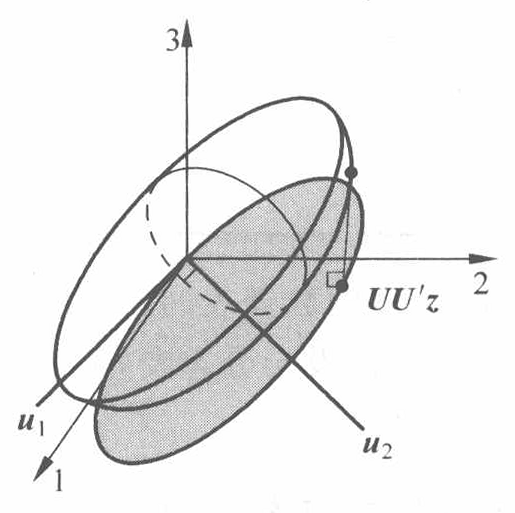
\includegraphics[width=43.6mm]{figs/fig_pg210_1.png}
\phantomsection\label{fig:5.13}\mvcap{图 5.13\quad 椭球 $\mathbf{z}'\mathbf{A}^{-1}\mathbf{z}\le c^2$ 在 $\mathbf{u}_1,\mathbf{u}_2$ 面上的投影为椭圆}
\end{mvfigure}

椭球在平面上的投影是最简单的, 当该平面由 $\mathbf{u}_1$, $\mathbf{u}_2$ 两向量确定时, 只要首先使这两单位向量彼此正交即可(见结论 2A.3).

\mvthm{结论 5A.3}{} 给定椭球 $\{\mathbf{z}:\mathbf{z}'\mathbf{A}^{-1}\mathbf{z}\le c^2\}$ 及两正交单位向量 $\mathbf{u}_1$ 和 $\mathbf{u}_2$, 则椭球 $\{\mathbf{z}:\mathbf{z}'\mathbf{A}^{-1}\mathbf{z}\le c^2\}$ 在 $\mathbf{u}_1,\mathbf{u}_2$ 平面上的投影是一椭圆 $\{(\mathbf{U}'\mathbf{z})'(\mathbf{U}'\mathbf{A}\mathbf{U})^{-1}(\mathbf{U}'\mathbf{z})\le c^2\}$, 其中, $\mathbf{U}=[\mathbf{u}_1:\mathbf{u}_2]$.

\mvbold{证明}\quad 由结论 2A.3, 向量 $\mathbf{z}$ 在 $\mathbf{u}_1,\mathbf{u}_2$ 平面上的投影为
\[
(\mathbf{u}_1'\mathbf{z})\mathbf{u}_1+(\mathbf{u}_2'\mathbf{z})\mathbf{u}_2
=[\mathbf{u}_1:\mathbf{u}_2]\begin{bmatrix}\mathbf{u}_1'\mathbf{z}\\\mathbf{u}_2'\mathbf{z}\end{bmatrix}
=\mathbf{U}\mathbf{U}'\mathbf{z}
\]
椭球 $\{\mathbf{z}:\mathbf{z}'\mathbf{A}^{-1}\mathbf{z}\le c^2\}$ 的投影为椭球中所有向量 $\mathbf{z}$ 在 $\mathbf{u}_1,\mathbf{u}_2$ 面上的投影, 即 $\mathbf{U}\mathbf{U}'\mathbf{z}$. 考虑投影 $\mathbf{U}(\mathbf{U}'\mathbf{z})$ 的两坐标 $\mathbf{U}'\mathbf{z}$. 设 $\mathbf{z}$ 属于椭球 $\{\mathbf{z}:\mathbf{z}'\mathbf{A}^{-1}\mathbf{z}\le c^2\}$, 则 $\mathbf{U}\mathbf{U}'\mathbf{z}$ 属于椭球的投影. 由结论 5A.2
\[
(\mathbf{U}'\mathbf{z})'(\mathbf{U}'\mathbf{A}\mathbf{U})^{-1}(\mathbf{U}'\mathbf{z})\le c^2
\]
故椭圆 $\{(\mathbf{U}'\mathbf{z})'(\mathbf{U}'\mathbf{A}\mathbf{U})^{-1}(\mathbf{U}'\mathbf{z})\le c^2\}$ 包含椭球投影的系数向量.

设 $\mathbf{U}a$ 为 $\mathbf{u}_1,\mathbf{u}_2$ 平面上一向量, 其系数 $a$ 属于椭圆 $\{a'(\mathbf{U}'\mathbf{A}\mathbf{U})^{-1}a\le c^2\}$. 若令 $\mathbf{z}=\mathbf{A}\mathbf{U}(\mathbf{U}'\mathbf{A}\mathbf{U})^{-1}a$, 则有
\[
\mathbf{U}'\mathbf{z}=\mathbf{U}'\mathbf{A}\mathbf{U}(\mathbf{U}'\mathbf{A}\mathbf{U})^{-1}a=a
\]
及
\[
\mathbf{z}'\mathbf{A}^{-1}\mathbf{z}=a'(\mathbf{U}'\mathbf{A}\mathbf{U})^{-1}\mathbf{U}'\mathbf{A}\mathbf{A}^{-1}\mathbf{A}\mathbf{U}(\mathbf{U}'\mathbf{A}\mathbf{U})^{-1}a=a'(\mathbf{U}'\mathbf{A}\mathbf{U})^{-1}a\le c^2
\]
因此, $\mathbf{U}'\mathbf{z}$ 属于系数向量椭圆, 且 $\mathbf{z}$ 属于椭球 $\mathbf{z}'\mathbf{A}^{-1}\mathbf{z}\le c^2$, 于是, 该椭圆只包含来自自由椭球 $\{\mathbf{z}:\mathbf{z}'\mathbf{A}^{-1}\mathbf{z}\le c^2\}$ 向 $\mathbf{u}_1,\mathbf{u}_2$ 平面的投影的系数向量. \hfill$\blacksquare$

\mvbold{评注}\quad 椭球先投影到 $\mathbf{u}_1,\mathbf{u}_2$ 平面, 然后再投影到 $\mathbf{u}_1$ 轴, 这与将椭球直接投影到 $\mathbf{u}_1$ 轴是一样的. 在讨论置信椭球时, 二维置信椭圆的投影给出单一分量的置信区间.

\mvbold{评注}\quad 若 $\mathbf{U}=[\mathbf{u}_1,\cdots,\mathbf{u}_q]$ 由 $q(2<q\le p)$ 个线性无关的列所组成, 则结论 5A.2 及结论 5A.3 仍成立.

\vspace{6pt}
{\large\bfseries 练习}

\medskip
\noindent 5.1\quad (a) 设数据 $\mathbf{X}=\begin{bmatrix}2&12\\8&9\\6&9\\8&10\end{bmatrix}$

%% ===== pg-211 =====

给定, 零假设为 $H_0:\boldsymbol{\mu}'=[7,11]$, 试计算 $T^2$.

(b)\ 确定 (a) 中 $T^2$ 的分布.

(c)\ 利用 (a) 与 (b), 在 $\alpha=0.05$ 水平下检验 $H_0$. 你得出什么结论?

\noindent 5.2\quad 利用例 5.1 的数据, 验证: 若将每个观测值 $\mathbf{x}_j$, $j=1,2,3$, 分别用 $\mathbf{C}\mathbf{x}_j$ 替代, 则 $T^2$ 保持不变. 此处
\[
\mathbf{C}=\begin{bmatrix}1&-1\\1&1\end{bmatrix}
\]
注意: 观测值
\[
\mathbf{C}\mathbf{x}_j=\begin{bmatrix}x_{j1}-x_{j2}\\x_{j1}+x_{j2}\end{bmatrix}
\]
产生的数据矩阵为:
\[
\begin{bmatrix}
(6-9)&(10-6)&(8-3)\\
(6+9)&(10+6)&(8+3)
\end{bmatrix}'
\]

\noindent 5.3\quad (a) 对练习 5.1 中的数据, 利用\hyperref[eq:5-15]{式(5-15)}计算 $T^2$.

(b)\ 用练习 5.1 的数据, 计算\hyperref[eq:5-13]{式(5-13)}中的 $\Lambda$, 并计算威尔克斯 $\Lambda$ 值.

\noindent 5.4\quad 利用\hyperref[tab:5.1]{表 5.1} 的汗液数据(见例 5.2)

(a)\ 确定 $\boldsymbol{\mu}$ 的 $90\%$ 置信椭球的主轴, 并计算其主轴的长度.

(b)\ 对排汗量、钠含量与钾含量的数据, 分别作 Q-Q 图, 并对每一对变量的观测值作散布图. 对这种情况, 多元正态假定是否合理? 试讨论.

\noindent 5.5\quad 对例 5.3 中的微波炉辐射数据给出的 $\bar{\mathbf{x}}$, $\mathbf{S}$ 及 $\mathbf{S}^{-1}$, 在显著性水平 $\alpha=0.05$ 下检验零假设 $H_0:\boldsymbol{\mu}'=[0.55,0.60]$, 所得结果是否与\hyperref[fig:5.1]{图 5.1} 中 $\boldsymbol{\mu}$ 的 $95\%$ 置信椭圆相一致? 请作出解释.

\noindent 5.6\quad 对 $m=3$ 验证庞弗罗尼不等\hyperref[eq:5-28]{式(5-28)}. 提示: 考虑三个事件 $C_1$, $C_2$ 与 $C_3$ 的韦恩图也许有帮助.

\noindent 5.7\quad 对\hyperref[tab:5.1]{表 5.1} 的汗液数据(见例 5.2), 利用结论 5.3 计算 $\mu_1$, $\mu_2$ 与 $\mu_3$ 的 $95\%$ 联合 $T^2$ 置信区间, 并用\hyperref[eq:5-29]{式(5-29)}构造其 $95\%$ 庞弗罗尼区间, 并对这两种区间进行比较.

\noindent 5.8\quad 从\hyperref[eq:5-23]{式(5-23)}我们知道, $T^2$ 等于由线性组合 $a'\bar{\mathbf{x}}$ 构造的一元 $t$ 值平方中的最大者, 此处 $a=\mathbf{S}^{-1}(\bar{\mathbf{x}}-\boldsymbol{\mu})$. 利用例 5.3 中的结论及练习 5.5 中的 $H_0$, 对变换后的微波炉辐射数据计算 $a$ 值. 验证: 由此 $a$ 值计算出的 $t^2$ 值等于练习 5.5 中的 $T^2$ 值.

\noindent 5.9\quad 为了维持大灰熊种群健康, 阿拉斯加州渔业和狩猎部的自然学家哈利·罗伯茨对大灰熊进行了研究. 在观测 61 只大灰熊的基础上, 他得到了如下的汇总统计数据(在练习 8.23 里也可看到):

\begin{center}
\begin{tabular}{lcccccc}
\toprule
变量 & 重量(kg) & 体长(cm) & 颈(cm) & 腰围(cm) & 头长(cm) & 头宽(cm)\\
\midrule
样本均值 $\bar{x}$ & 95.52 & 164.38 & 55.69 & 93.39 & 17.98 & 31.13\\
\bottomrule
\end{tabular}
\end{center}

协方差矩阵为:
\[
\mathbf{S}=\begin{bmatrix}
3266.46&1343.97&731.54&1175.50&162.68&238.37\\
1343.97&721.91&324.25&537.35&80.17&117.73\\
731.54&324.25&179.28&281.17&39.15&56.80\\
1175.50&537.35&281.17&474.98&63.73&94.85\\
162.68&80.17&39.15&63.73&9.95&13.88\\
238.37&117.73&56.80&94.85&13.88&21.26
\end{bmatrix}
\]

%% ===== pg-212 =====

(a)\ 求大灰熊的身体观测数据的六个总体均值的大样本 $95\%$ 联合置信区间.

(b)\ 求体重和腰围的均值的大样本 $95\%$ 联合置信椭圆.

(c)\ 求在 (a) 中的六个均值的大样本 $95\%$ 庞弗罗尼置信区间.

(d)\ 参考 (b), 对 $m=6$ 构造重量和腰围均值的 $95\%$ 庞弗罗尼置信矩形, 并和 (b) 中的置信椭圆进行比较.

(e)\ 对 $m=6+1=7$(所有单个均值的表述), 求头宽均值—头长均值的 $95\%$ 庞弗罗尼置信区间.

\noindent 5.10\quad 参考例 1.10 (见\hyperref[tab:1.4]{表 1.4}) 中的熊的成长数据. 关注体长观测值.

(a)\ 求四个总体的体长均值的 $95\%$ $T^2$ 联合置信区间.

(b)\ 参考 (a), 求体长均值的相继三年的年增长的 $95\%$ $T^2$ 联合置信区间.

(c)\ 求从 2 岁到 3 岁的体长的增长均值以及 4 岁到 5 岁的体长的增长均值的 $95\%$ $T^2$ 置信椭圆.

(d)\ 参考 (a) 和 (b), 构造包含四个体长均值以及体长均值的相继三年的年增长的集合的 $95\%$ 庞弗罗尼置信区间.

(e)\ 参考 (c) 和 (d), 将从 2 岁到 3 岁的体长的增长均值以及 4 岁到 5 岁的体长的增长均值的 $95\%$ 庞弗罗尼置信矩形和与 $T^2$ 方法得到的置信椭圆进行比较.

\noindent 5.11\quad 一名人类学家对 9 根古秘鲁人头发的头发完成了矿物分析, 测得其中的铬(Cr)含量 $x_1$ 和锶(Sr)含量 $x_2$(单位为 p.p.m, 即百万分之一)分别为

\begin{center}
\begin{tabular}{lccccccccc}
\toprule
$x_1$(Cr) & 0.48 & 40.53 & 2.19 & 0.55 & 0.74 & 0.66 & 0.93 & 0.37 & 0.22\\
$x_2$(Sr) & 12.57 & 73.68 & 11.13 & 20.03 & 20.29 & 0.78 & 4.64 & 0.43 & 1.08\\
\bottomrule
\end{tabular}
\end{center}

已知铬含量较低(低于或等于 0.100 p.p.m)可能是糖尿病的表现, 而锶含量的高低则说明动物蛋白摄入的多少.

(a)\ 假定这 9 根秘鲁人头发代表一个来自属于某种特定古秘鲁文化的随机样本. 试构造并画出总体均值向量 $\boldsymbol{\mu}'=[\mu_1,\mu_2]$ 的 $90\%$ 联合置信椭圆.

(b)\ 用 (a) 中构造的椭圆向每一坐标轴投影, 求出 $\mu_1$ 与 $\mu_2$ 的 $90\%$ 联合置信区间(可利用结论 5.3). 是否有迹象表明这种古秘鲁人头发的平均锶含量为 10? 也就是说, 所有的点(任意 $\mu$ 值, 10)是否都在置信域中? $[0.30,10]$ 是否为 $\boldsymbol{\mu}$ 的真值? 试作讨论.

(c)\ 这些数据是否显示出二元正态性? 利用 Q-Q 图与散布图来考察这个问题. 若数据没有二元正态性, 那么 (a) 与 (b) 中的结论又意味着什么?

(d)\ 摒弃明显的离群观测值后重新进行分析, 推断是否会有所改变? 试作评论.

\noindent 5.12\quad 设有若干个分量缺损的观测数据为
\[
\mathbf{X}=\begin{bmatrix}
3&6&0\\
4&4&3\\
-&8&3\\
5&-&-
\end{bmatrix}
\]
试用 5.7 节中的预测-估计算法估计 $\boldsymbol{\mu}$ 和 $\boldsymbol{\Sigma}$, 要求给出其初始估计值及一步迭代的修正估计值.

\noindent 5.13\quad 对\hyperref[tab:5.1]{表 5.1} 的汗液数据确定 $-n\ln(|\hat{\boldsymbol{\Sigma}}|/|\hat{\boldsymbol{\Sigma}}_0|)$ 的近似分布(参见结论 5.2).

\noindent 5.14\quad 试建立一个类似于\hyperref[tab:5.4]{表 5.4} 的新表, 表中的元素为(单一 $t$ 区间)的宽度/(庞弗罗尼 $t$

%% ===== pg-213 =====

区间的宽度).

练习 5.15, 5.16 和 5.17 需要用到下面的知识:

人们感兴趣的总体特征通常全部或部分地表现为一些属性, 这时总体中的每一个体可用它所具有的属性来描述. 为方便起见, 通常将属性按它们的存在与否进行数量化编码. 若以变量 $X$ 代表某一特定属性, 我们便可通过如下定义来区别此种属性的有无:
\[
X=\begin{cases}
1 & \text{该属性存在}\\
0 & \text{该属性不存在}
\end{cases}
\]
用这种方式, 我们就能给性质特征指定数值.

当属性用 0—1 变量进行数量化编码时, 来自我们感兴趣总体的随机样本将导致两种不同计数, 每一种代表具有不同特征的样本项目数. 如果样本计数很大, 不难将产生联合置信表示方法改写为适合包括比例在内的情形.

考虑这样一种情形: 一个具有某种特定属性组合的个体可归入 $q+1$ 个互斥完备类之一, 相应的概率分别为 $p_1,p_2,\cdots,p_q,p_{q+1}$. 因为这些类别包含了所有各种可能性, 所以 $p_{q+1}=1-(p_1+p_2+\cdots+p_q)$. 来自第 $k$ 类的个体对应一个 $[(q+1)\times1]$ 向量 $[0,\cdots,0,1,0,\cdots,0]'$, 其中 1 出现在第 $k$ 个位置.

我们知道, 来自由 $q+1$ 个互斥完备类中的个体组成的总体的样本观测值, 其概率分布为多项分布, 并有如下结构:

\begin{center}
\begin{tabular}{lccccccc}
\toprule
类别: & 1 & 2 & $\cdots$ & $k$ & $\cdots$ & $q$ & $q+1$\\
\midrule
结果: &
$\begin{bmatrix}1\\0\\0\\\vdots\\0\\\vdots\\0\end{bmatrix}$ &
$\begin{bmatrix}0\\1\\0\\\vdots\\0\\\vdots\\0\end{bmatrix}$ &
$\cdots$ &
$\begin{bmatrix}0\\0\\\vdots\\1\\0\\\vdots\\0\end{bmatrix}$ &
$\cdots$ &
$\begin{bmatrix}0\\0\\\vdots\\0\\1\\\vdots\\0\end{bmatrix}$ &
$\begin{bmatrix}0\\0\\\vdots\\0\\\vdots\\1\end{bmatrix}$\\
\midrule
概率(比例): & $p_1$ & $p_2$ & $\cdots$ & $p_k$ & $\cdots$ & $p_q$ & $p_{q+1}=1-\sum\limits_{i=1}^{q}p_i$\\
\bottomrule
\end{tabular}
\end{center}

设 $\mathbf{X}_j$, $j=1,2,\cdots,n$ 为来自多项分布总体的一个容量为 $n$ 的随机样本. 若样本观测值(个体)来自第 $k$ 类, 则 $\mathbf{X}_j$ 的第 $k$ 个分量 $X_{jk}=1$, 否则为 0.

随机样本 $\mathbf{X}_1,\mathbf{X}_2,\cdots,\mathbf{X}_n$ 可变换成一个样本比例向量, 该向量就前面数据的性质而论是一样本均值向量, 故
\[
\hat{\mathbf{p}}=\begin{bmatrix}\hat{p}_1\\\hat{p}_2\\\vdots\\\hat{p}_{q+1}\end{bmatrix}
=\frac{1}{n}\sum_{j=1}^{n}\mathbf{X}_j, \quad
E(\hat{\mathbf{p}})=\mathbf{p}=\begin{bmatrix}p_1\\p_2\\\vdots\\p_{q+1}\end{bmatrix}
\]
及
\[
\mathrm{Cov}(\hat{\mathbf{p}})=\frac{1}{n}\mathrm{Cov}(\mathbf{X}_j)=\frac{1}{n}\boldsymbol{\Sigma}
=\frac{1}{n}\begin{bmatrix}
\sigma_{11}&\sigma_{12}&\cdots&\sigma_{1,q+1}\\
\sigma_{21}&\sigma_{22}&\cdots&\sigma_{2,q+1}\\
\vdots&\vdots&&\vdots\\
\sigma_{q+1,1}&\sigma_{q+1,2}&\cdots&\sigma_{q+1,q+1}
\end{bmatrix}
\]

%% ===== pg-214 =====

当 $n$ 充分大时, 中心极限定理给出 $\hat{\mathbf{p}}$ 的近似抽样分布, 即有
\[
\sqrt{n}(\hat{\mathbf{p}}-\mathbf{p})\ \text{近似服从分布}\ N(\mathbf{0},\boldsymbol{\Sigma})
\]
其中 $\boldsymbol{\Sigma}$ 的元素为 $\sigma_{kk}=p_k(1-p_k)$, $\sigma_{ik}=-p_ip_k$. 当 $\sigma_{kk}$ 用 $\hat{\sigma}_{kk}=\hat{p}_k(1-\hat{p}_k)$ 来估计, $\sigma_{ik}$ 用 $\hat{\sigma}_{ik}=-\hat{p}_i\hat{p}_k$, $i\ne k$ 来估计时, 正态近似仍有效.

由于每一个体属于且仅属于某一类, 故 $X_{q+1,j}=1-(X_{1j}+X_{2j}+\cdots+X_{qj})$, 从而 $\hat{p}_{q+1}=1-(\hat{p}_1+\hat{p}_2+\cdots+\hat{p}_q)$ 且 $\boldsymbol{\Sigma}$ 的秩为 $q$. 尽管此时 $\boldsymbol{\Sigma}$ 的逆阵不存在, 但我们仍可构造所有线性组合 $\mathbf{a}'\mathbf{p}$ 的 $100(1-\alpha)\%$ 联合置信区间.

\mvthm{结论}{} 设 $\mathbf{X}_1,\mathbf{X}_2,\cdots,\mathbf{X}_n$ 为来自具有 $q+1$ 类的多项分布总体, $P[X_{jk}=1]=p_k$, $k=1,2,\cdots,q+1$, $j=1,2,\cdots,n$, 假如 $n-q$ 充分大, 那么, 对所有线性组合 $\mathbf{a}'\mathbf{p}=a_1p_1+a_2p_2+\cdots+a_{q+1}p_{q+1}$, 其近似的 $100(1-\alpha)\%$ 联合置信区间为
\[
\mathbf{a}'\hat{\mathbf{p}}\pm\sqrt{\chi_q^2(\alpha)}\sqrt{\frac{\mathbf{a}'\hat{\boldsymbol{\Sigma}}\mathbf{a}}{n}}
\]
其中 $\hat{\mathbf{p}}=(1/n)\sum\limits_{j=1}^{n}\mathbf{X}_j$, 且 $\hat{\boldsymbol{\Sigma}}=(\hat{\sigma}_{ik})$ 是一个 $(q+1)\times(q+1)$ 矩阵, 满足 $\hat{\sigma}_{kk}=\hat{p}_k(1-\hat{p}_k)$ 与 $\hat{\sigma}_{ik}=-\hat{p}_i\hat{p}_k$, $i\ne k$, 而 $\chi_q^2(\alpha)$ 则为自由度为 $q$ 的 $\chi^2$ 分布的上 $100\alpha$ 百分位数. \hfill$\blacksquare$

在此结论中, 要求 $n-q$ 充分大可理解为对每一类有 $n\hat{p}_k\ge20$.

在这里, 我们仅略微涉及分析分类数据的可能性问题, 对这个问题的完整讨论, 读者可从文献[1]与文献[4]中得到.

\noindent 5.15\quad 设 $X_{ji}$ 和 $X_{jk}$ 分别为 $\mathbf{X}_j$ 的第 $i$ 个分量与第 $k$ 个分量.

(a)\ 证明 $\mu_k=E(X_{jk})=p_k$, $\sigma_{kk}=\mathrm{Var}(X_{jk})=p_k(1-p_k)$, $k=1,2,\cdots,p$.

(b)\ 证明 $\sigma_{ik}=\mathrm{Cov}(X_{ji},X_{jk})=-p_ip_k$, $i\ne k$. 并说明此协方差为何必为负值.

\noindent 5.16\quad 作为一个大型市场营销研究项目的一部分, 谢尔伍德银行的一名顾问想知道把银行存款作为主要储蓄手段的储户的比例. 此外, 他还想知道这家银行的三个主要竞争对手(银行 B, C 和 D)的上述储户的比例. 在一项调查中, 每个被调查者回答了下面的问题:

哪家银行是您的主要储蓄银行?

回答

\begin{center}
\mvfit{%
\begin{tabular}{|c|c|c|c|c|c|}
\hline
谢尔伍德银行 & 银行 B & 银行 C & 银行 D & 其他银行 & 没有存款\\
\hline
\end{tabular}
}
\end{center}

当被问及主要的储蓄银行时, 被调查的 $n=355$ 名有储蓄账户者的回答统计如下(没有存款的在存户比较中被忽略, 故总共只有 5 类):

\begin{center}
\mvfit{%
\begin{tabular}{lccccc}
\toprule
银行(分类) & 谢尔伍德银行 & 银行 B & 银行 C & 银行 D & 其他银行\\
\midrule
考察人数 & 105 & 119 & 56 & 25 & 50\ \ 总人数 $n=355$\\
总体比例 & $p_1$ & $p_2$ & $p_3$ & $p_4$ & $p_5=1-(p_1+p_2+p_3+p_4)$\\
样本比例 & $\hat{p}_1=\dfrac{105}{355}=0.30$ & $\hat{p}_2=0.33$ & $\hat{p}_3=0.16$ & $\hat{p}_4=0.07$ & $\hat{p}_5=0.14$\\
\bottomrule
\end{tabular}
}
\end{center}

%% ===== pg-215 =====

设总体比例为
\begin{align*}
p_{1}&=\text{在谢尔伍德银行存款的储户的比例}\\
p_{2}&=\text{在银行 B 存款的储户的比例}\\
p_{3}&=\text{在银行 C 存款的储户的比例}\\
p_{4}&=\text{在银行 D 存款的储户的比例}\\
1-(p_{1}&+p_{2}+p_{3}+p_{4})=\text{在其他银行存款的储户的比例}
\end{align*}

(a) 求 $p_{1},p_{2},\cdots,p_{4}$ 的 $95\%$ 联合置信区间

(b) 构造一个可将谢尔伍德银行与其主要竞争对手 B 进行比较的 $95\%$ 联合置信区间, 并对这一区间作出解释.

\medskip
\noindent\mvbold{5.17}\quad 为评估某城市高中学生中吸毒问题的普遍性, 对来自该城市 5 所高中的 200 名学生所组成的一个随机样本进行了调查, 调查的问题之一及相应的回答如下:

通常您一周吸几支大麻烟?

\begin{mvtable}
\centering
\begin{tabular}{|c|c|c|c|}
\hline
\multirow{2}{*}{} & \multicolumn{3}{c|}{分类}\\
\cline{2-4}
 & 不吸 & 中等 ($1\sim3$ 支) & 严重 ($4$ 支以上)\\
\hline
应答人数 & $117$ & $62$ & $21$\\
\hline
\end{tabular}
\end{mvtable}

试对这三种人的比例 $p_{1},p_{2}$ 与 $p_{3}=1-(p_{1}+p_{2})$ 构造 $95\%$ 联合置信区间.

\medskip
\noindent\mvbold{下面的练习需要使用计算机.}

\medskip
\noindent\mvbold{5.18}\quad 利用\hyperref[tab:5.2]{表 5.2} 中的大学考试数据 (见例 5.5)

\noindent (a) 在显著性水平 $\alpha=0.05$ 下检验假设
\[
H_{0}:\boldsymbol{\mu}'=[500,50,30],\quad H_{1}:\boldsymbol{\mu}'\ne[500,50,30]
\]
假定 $[500,50,30]'$ 代表近 10 年来数千名大学生考试的平均成绩. 是否有理由相信, 成绩被列入\hyperref[tab:5.2]{表 5.2} 的那一组学生与以往的学生相比其得分情况有明显不同? 请作出解释.

\noindent (b) 确定 $\boldsymbol{\mu}$ 的 $95\%$ 置信椭球的主轴的长度与方向.

\noindent (c) 从社会科学与历史、语言表达以及自然科学各科成绩的边缘分布画出 Q-Q 图. 从各对不同变量的观测值中画出可能的三个散布图. 讨论这些数据是否服从正态分布.

\medskip
\noindent\mvbold{5.19}\quad \hyperref[tab:5.11]{表 5.11} 中给出由 $n=30$ 根一等硬木组成的样本的硬度 $x_{1}$ 与弯曲强度 $x_{2}$ 的测量值, 单位为磅/英寸$^{2}$. 利用表中数据:

\begin{mvtable}
\phantomsection\label{tab:5.11}\mvtabcap{表 5.11\quad 木材数据}
\centering
\begin{tabular}{|c|c||c|c|}
\hline
$x_{1}$(硬度) & $x_{2}$(弯曲强度) & $x_{1}$(硬度) & $x_{2}$(弯曲强度)\\
\hline
$1\,232$ & $4\,175$ & $1\,712$ & $7\,749$\\
$1\,115$ & $6\,652$ & $1\,932$ & $6\,818$\\
$2\,205$ & $7\,612$ & $1\,820$ & $9\,307$\\
$1\,897$ & $10\,914$ & $1\,900$ & $6\,457$\\
$1\,932$ & $10\,850$ & $2\,426$ & $10\,102$\\
$1\,612$ & $7\,627$ & $1\,558$ & $7\,414$\\
$1\,598$ & $6\,954$ & $1\,470$ & $7\,556$\\
$1\,804$ & $8\,365$ & $1\,858$ & $7\,833$\\
\hline
\end{tabular}
\end{mvtable}

%% ===== pg-216 =====

\begin{mvtable}
\centering
{\small 续表}\\[2pt]
\begin{tabular}{|c|c||c|c|}
\hline
$x_{1}$(硬度) & $x_{2}$(弯曲强度) & $x_{1}$(硬度) & $x_{2}$(弯曲强度)\\
\hline
$1\,752$ & $9\,469$ & $1\,587$ & $8\,309$\\
$2\,067$ & $6\,410$ & $2\,208$ & $9\,559$\\
$2\,365$ & $10\,327$ & $1\,487$ & $6\,255$\\
$1\,646$ & $7\,320$ & $2\,206$ & $10\,723$\\
$1\,579$ & $8\,196$ & $2\,332$ & $5\,430$\\
$1\,880$ & $9\,709$ & $2\,540$ & $12\,090$\\
$1\,773$ & $10\,370$ & $2\,322$ & $10\,072$\\
\hline
\end{tabular}\\[3pt]
{\footnotesize 资料来源: 数据经美国林业制品实验室许可使用.}
\end{mvtable}

\noindent (a) 构造并画出 $[\mu_{1},\mu_{2}]'$ 的 $95\%$ 置信椭圆, 其中 $\mu_{1}=E(X_{1}),\mu_{2}=E(X_{2})$.

\noindent (b) 假设硬度及弯曲强度的“标准”值分别为 $\mu_{10}=2\,000$ 及 $\mu_{20}=10\,000$, 已知 (a) 的结论, 讨论\hyperref[tab:5.11]{表 5.11} 中的数据是否与这些数值相容.

\noindent (c) 用 Q-Q 图及散布图来解释二维正态分布是否为该总体的一个可行的模型.

\medskip
\noindent\mvbold{5.20}\quad 一位野生动物生态学家对一个由 $n=45$ 只雄性钩镰鸢组成的样本测量了两项指标: $x_{1}=$ 尾长 (毫米), $x_{2}=$ 翅长 (毫米), 数据列于\hyperref[tab:5.12]{表 5.12}.

\begin{mvtable}
\phantomsection\label{tab:5.12}\mvtabcap{表 5.12\quad 钩镰鸢数据}
\centering
{\small
\begin{tabular}{|c|c|c|c|c|c|}
\hline
$x_{1}$ & $x_{2}$ & $x_{1}$ & $x_{2}$ & $x_{1}$ & $x_{2}$\\
(尾长) & (翅长) & (尾长) & (翅长) & (尾长) & (翅长)\\
\hline
$191$ & $284$ & $186$ & $266$ & $173$ & $271$\\
$197$ & $285$ & $197$ & $285$ & $194$ & $280$\\
$208$ & $288$ & $201$ & $295$ & $198$ & $300$\\
$180$ & $273$ & $190$ & $282$ & $180$ & $272$\\
$180$ & $275$ & $209$ & $305$ & $190$ & $292$\\
$188$ & $280$ & $187$ & $285$ & $191$ & $286$\\
$210$ & $283$ & $207$ & $297$ & $196$ & $285$\\
$196$ & $288$ & $178$ & $268$ & $207$ & $286$\\
$191$ & $271$ & $202$ & $271$ & $209$ & $303$\\
$179$ & $257$ & $205$ & $285$ & $179$ & $261$\\
$208$ & $289$ & $190$ & $280$ & $186$ & $262$\\
$202$ & $285$ & $189$ & $277$ & $174$ & $245$\\
$200$ & $272$ & $211$ & $310$ & $181$ & $250$\\
$192$ & $282$ & $216$ & $305$ & $189$ & $262$\\
$199$ & $280$ & $189$ & $274$ & $188$ & $258$\\
\hline
\end{tabular}}\\[3pt]
{\footnotesize 资料来源: 数据经 S. Temple 许可使用.}
\end{mvtable}

利用表中的数据:

\noindent (a) 构造并画出总体均值 $\mu_{1}$ 和 $\mu_{2}$ 的 $95\%$ 置信椭圆, 假定雄性钩镰鸢的 $\mu_{1}=190$ 毫米, $\mu_{2}=275$ 毫米. 试问这些值是否为雄性钩镰鸢的平均尾长和平均翅膀长的真值? 请予以解释.

%% ===== pg-217 =====

\noindent (b) 试作出 $\mu_{1}$ 和 $\mu_{2}$ 的 $95\%$ 联合 $T^{2}$ 区间及庞弗罗尼区间, 并将这两种区间进行比较. $T^{2}$ 区间是否比庞弗罗尼区间更优越 (如果有优越性的话)?

\noindent (c) 二元正态分布是可行的总体模型吗? 试用 Q-Q 图和散布图来解释.

\medskip
\noindent\mvbold{5.21}\quad 利用\hyperref[tab:1.8]{表 1.8} 中的数据, 构造其各均值的 $95\%$ 庞弗罗尼区间, 以及 $95\%$ 联合 $T^{2}$ 区间, 并对这两个区间进行比较.

\medskip
\noindent\mvbold{5.22}\quad 复制第 6 章\hyperref[tab:6.10]{表 6.10} 中的部分数据 (\hyperref[tab:5.13]{表 5.13}). 这些数据代表用卡车把牛奶从农场运到奶制品厂的各种运输成本. \hyperref[tab:6.10]{表 6.10} 只给出了卡车的前 25 个多元观测值. 第 9 个和第 21 个观测值是由 36 个观测值组成的整个数据集中的两个离群值 (见文献 [2]).

\begin{mvtable}
\phantomsection\label{tab:5.13}\mvtabcap{表 5.13\quad 牛奶运输价格数据}
\centering
{\small
\begin{tabular}{|c|c|c||c|c|c|}
\hline
燃料($x_{1}$) & 维修($x_{2}$) & 资金($x_{3}$) & 燃料($x_{1}$) & 维修($x_{2}$) & 资金($x_{3}$)\\
\hline
$16.44$ & $12.43$ & $11.23$ & $11.11$ & $6.15$ & $7.61$\\
$7.19$ & $2.70$ & $3.92$ & $12.17$ & $14.26$ & $14.39$\\
$9.92$ & $1.35$ & $9.75$ & $10.24$ & $2.59$ & $6.09$\\
$4.24$ & $5.78$ & $7.78$ & $10.18$ & $6.05$ & $12.14$\\
$11.20$ & $5.05$ & $10.67$ & $8.88$ & $2.70$ & $12.23$\\
$14.25$ & $5.78$ & $9.88$ & $12.34$ & $7.73$ & $11.68$\\
$13.50$ & $10.98$ & $10.60$ & $8.51$ & $14.02$ & $12.01$\\
$13.32$ & $14.27$ & $9.45$ & $26.16$ & $17.44$ & $16.89$\\
$29.11$ & $15.09$ & $3.28$ & $12.95$ & $8.24$ & $7.18$\\
$12.68$ & $7.61$ & $10.23$ & $16.93$ & $13.37$ & $17.59$\\
$7.51$ & $5.80$ & $8.13$ & $14.70$ & $10.78$ & $14.58$\\
$9.90$ & $3.63$ & $9.13$ & $10.32$ & $5.16$ & $17.00$\\
$10.25$ & $5.07$ & $10.17$ & & &\\
\hline
\end{tabular}}
\end{mvtable}

\noindent (a) 试作燃料成本、维修成本与资金成本的边缘分布的 Q-Q 图, 并作出各对不同变量观测值之间的三个可能的散布图. 有无明显的离群值? 摒弃离群值后, 重新绘制 Q-Q 图及散布图, 试讨论现在的数据是否服从正态分布.

\noindent (b) 求成本均值的 $95\%$ 庞弗罗尼区间及 $T^{2}$ 区间, 并对它们进行比较.

\medskip
\noindent\mvbold{5.23}\quad 考虑\hyperref[tab:6.13]{表 6.13} 中的第一时段的 30 个古埃及男性头骨观测值.

\noindent (a) 构造头骨的最大宽度, 头骨的高度, 头骨底穴至齿槽的长度和头骨鼻梁高度这些变量的边缘分布的 Q-Q 图. 另外, 构造一个多元观测的 $\chi^{2}$ 图. 这些数据服从正态分布吗? 请解释原因.

\noindent (b) 构造个体头骨尺寸变量的 $95\%$ 庞弗罗尼区间. 另外, 找出它的 $95\%$ $T^{2}$ 区间. 比较这两个区间.

\medskip
\noindent\mvbold{5.24}\quad 利用\hyperref[tab:5.8]{表 5.8} 中的麦迪逊警署数据, 构造 $x_{1}$ 和 $x_{2}$ 的个别 $\bar{X}$ 控制图. 试问这两个过程是否都处在受控状态 (即是否稳定)?

\medskip
\noindent\mvbold{5.25}\quad 参看练习 5.24. 利用 $x_{2}$ 与 $x_{1}$ 的数据, 作出它们的质量控制椭圆及 $T^{2}$ 控制图. 这些二元观测值所代表的过程是否处在受控状态? 试作出评论. 从多元控制图中, 你是否学到了某些在个别 $\bar{X}$ 控制图中没有的东西?

\medskip
\noindent\mvbold{5.26}\quad 利用\hyperref[tab:5.8]{表 5.8} 中的 $x_{1},x_{2}$ 及 $x_{3}$ 的数据构造一个 $T^{2}$ 控制图, 将此图与例 5.10 中的

%% ===== pg-218 =====

\hyperref[fig:5.8]{图 5.8} 进行比较. 添加一个特征后给出的 $T^{2}$ 控制图是否改变了你对过程稳定性的结论? 请解释.

\medskip
\noindent\mvbold{5.27}\quad 用\hyperref[tab:5.8]{表 5.8} 中 $x_{3}$ 与 $x_{4}$ 的数据, 构造未来观测值 $\mathbf{x}'=(x_{3},x_{4})$ 的预测椭圆. 注意, 预测椭圆必须从稳定过程出发求得. 对所得结果作出解释.

\medskip
\noindent\mvbold{5.28}\quad 作为金属片装配过程研究的一部分, 一个大的汽车制造商在汽车的六个位置使用传感器来记录与名义上的厚度的偏离 (mm). 前四个是当汽车主体完成时测量的, 后两个是装配早期在汽车底部测量的. 基于 50 辆汽车的数据见\hyperref[tab:5.14]{表 5.14}.

\noindent (a) 装配过程对于前 30 个看起来是稳定的. 用这些数据来估计 $\mathbf{S}$ 和 $\bar{\mathbf{x}}$. 然后用所有的数据 (50 个) 构造一个 $T^{2}$ 控制图.

\noindent (b) 哪一个位置看起来是需要找原因的?

\begin{mvtable}
\phantomsection\label{tab:5.14}\mvtabcap{表 5.14\quad 车体装配数据}
\centering
{\small
\begin{tabular}{|r|r|r|r|r|r|r|}
\hline
编号 & $x_{1}$ & $x_{2}$ & $x_{3}$ & $x_{4}$ & $x_{5}$ & $x_{6}$\\
\hline
$1$ & $-0.12$ & $0.36$ & $0.40$ & $0.25$ & $1.37$ & $-0.13$\\
$2$ & $-0.60$ & $-0.35$ & $0.04$ & $-0.28$ & $-0.25$ & $-0.15$\\
$3$ & $-0.13$ & $0.05$ & $0.84$ & $0.61$ & $1.45$ & $0.25$\\
$4$ & $-0.46$ & $-0.37$ & $0.30$ & $0.00$ & $-0.12$ & $-0.25$\\
$5$ & $-0.46$ & $-0.24$ & $0.37$ & $0.13$ & $0.78$ & $-0.15$\\
$6$ & $-0.46$ & $-0.16$ & $0.07$ & $0.10$ & $1.15$ & $-0.18$\\
$7$ & $-0.46$ & $-0.24$ & $0.13$ & $0.02$ & $0.26$ & $-0.20$\\
$8$ & $-0.13$ & $0.05$ & $-0.01$ & $0.09$ & $-0.15$ & $-0.18$\\
$9$ & $-0.31$ & $-0.16$ & $-0.20$ & $0.23$ & $0.65$ & $0.15$\\
$10$ & $-0.37$ & $-0.24$ & $0.37$ & $0.21$ & $1.15$ & $0.05$\\
$11$ & $-1.08$ & $-0.83$ & $-0.81$ & $0.05$ & $0.21$ & $0.00$\\
$12$ & $-0.42$ & $-0.30$ & $0.37$ & $-0.58$ & $0.00$ & $-0.45$\\
$13$ & $-0.31$ & $0.10$ & $-0.24$ & $0.24$ & $0.65$ & $0.35$\\
$14$ & $-0.14$ & $0.06$ & $0.18$ & $-0.50$ & $1.25$ & $0.05$\\
$15$ & $-0.61$ & $-0.35$ & $-0.24$ & $0.75$ & $0.15$ & $-0.20$\\
$16$ & $-0.61$ & $-0.30$ & $-0.20$ & $-0.21$ & $-0.50$ & $-0.25$\\
$17$ & $-0.84$ & $-0.35$ & $-0.14$ & $-0.22$ & $1.65$ & $-0.05$\\
$18$ & $-0.96$ & $-0.85$ & $0.19$ & $-0.18$ & $1.00$ & $-0.08$\\
$19$ & $-0.90$ & $-0.34$ & $-0.78$ & $-0.15$ & $0.25$ & $0.25$\\
$20$ & $-0.46$ & $0.36$ & $0.24$ & $-0.58$ & $0.15$ & $0.25$\\
$21$ & $-0.90$ & $-0.59$ & $0.13$ & $-0.58$ & $0.60$ & $-0.08$\\
$22$ & $-0.61$ & $-0.50$ & $-0.34$ & $-0.58$ & $0.95$ & $-0.08$\\
$23$ & $-0.61$ & $-0.20$ & $-0.58$ & $-0.20$ & $1.10$ & $0.00$\\
$24$ & $-0.46$ & $-0.30$ & $-0.10$ & $-0.10$ & $0.75$ & $-0.10$\\
$25$ & $-0.60$ & $-0.35$ & $-0.45$ & $0.37$ & $1.18$ & $-0.30$\\
$26$ & $-0.60$ & $-0.36$ & $-0.34$ & $-0.11$ & $1.68$ & $-0.32$\\
$27$ & $-0.31$ & $0.35$ & $-0.45$ & $-0.10$ & $1.00$ & $-0.25$\\
$28$ & $-0.60$ & $-0.25$ & $-0.42$ & $0.28$ & $0.75$ & $0.10$\\
$29$ & $-0.31$ & $0.25$ & $-0.34$ & $-0.24$ & $0.65$ & $0.10$\\
\hline
\end{tabular}}
\end{mvtable}

%% ===== pg-219 =====

\begin{mvtable}
\mvtabcap{续表}
\begin{tabular}{ccccccc}
\toprule
编号 & $x_1$ & $x_2$ & $x_3$ & $x_4$ & $x_5$ & $x_6$\\
\midrule
30 & $-0.36$ & $-0.16$ & $0.15$ & $-0.38$ & $1.18$ & $-0.10$\\
31 & $-0.40$ & $-0.12$ & $-0.48$ & $-0.34$ & $0.30$ & $-0.20$\\
32 & $-0.60$ & $-0.40$ & $-0.20$ & $0.32$ & $0.50$ & $0.10$\\
33 & $-0.47$ & $-0.16$ & $-0.34$ & $-0.31$ & $0.85$ & $0.60$\\
34 & $-0.46$ & $-0.18$ & $0.16$ & $0.01$ & $0.60$ & $0.35$\\
35 & $-0.44$ & $-0.12$ & $-0.20$ & $-0.48$ & $1.40$ & $0.10$\\
36 & $-0.90$ & $-0.40$ & $0.75$ & $-0.31$ & $0.60$ & $-0.10$\\
37 & $-0.50$ & $-0.35$ & $0.84$ & $-0.52$ & $0.35$ & $-0.75$\\
38 & $-0.38$ & $0.08$ & $0.55$ & $-0.15$ & $0.80$ & $-0.10$\\
39 & $-0.60$ & $-0.35$ & $-0.35$ & $-0.34$ & $0.60$ & $0.85$\\
40 & $0.11$ & $0.24$ & $0.15$ & $0.40$ & $0.00$ & $-0.10$\\
41 & $0.05$ & $0.12$ & $0.85$ & $0.55$ & $1.65$ & $-0.10$\\
42 & $-0.85$ & $-0.65$ & $0.50$ & $0.35$ & $0.80$ & $-0.21$\\
43 & $-0.37$ & $-0.10$ & $-0.10$ & $-0.58$ & $1.85$ & $-0.11$\\
44 & $-0.11$ & $0.24$ & $0.75$ & $-0.10$ & $0.65$ & $-0.10$\\
45 & $-0.60$ & $-0.24$ & $0.13$ & $0.84$ & $0.85$ & $0.15$\\
46 & $-0.84$ & $-0.59$ & $0.05$ & $0.61$ & $1.00$ & $0.20$\\
47 & $-0.46$ & $-0.16$ & $0.37$ & $-0.15$ & $0.68$ & $0.25$\\
48 & $-0.56$ & $-0.35$ & $-0.10$ & $0.75$ & $0.45$ & $0.20$\\
49 & $-0.56$ & $-0.16$ & $0.37$ & $-0.25$ & $1.05$ & $0.15$\\
50 & $-0.25$ & $-0.12$ & $-0.05$ & $-0.20$ & $1.21$ & $0.10$\\
\bottomrule
\end{tabular}
\end{mvtable}

资料来源：数据经 Darek Ceglarek 许可使用.

\noindent 5.29\quad 参考练习 5.28 中的车体数据.这些数据都是作为目标值的离差测量的,所以用来检验均值向量为零的零假设是合适的.使用前 30 个数据,在水平 $\alpha=0.05$ 下,检验 $H_0$: $\boldsymbol{\mu}=\mathbf{0}$.

\noindent 5.30\quad 参考练习 3.18 中的能量消耗的数据.

(a) 对 4 种类型中的每一种能源的平均消耗,它们的平均总消耗量和汽油减去天然气的平均差,求大样本的 95\% 庞弗罗尼置信区间.

(b) 对 4 种类型中的每一种能源的平均消耗,它们的平均总消耗量和汽油减去天然气的平均差,求大样本的 95\% 联合 $T^2$ 区间.并与 (a) 中的结果进行比较.

\noindent 5.31\quad 参考练习 3.20 中的暴风雪数据.

(a) 做一些合适的变换之后,找出均值向量的 95\% 的置信域.

(b) 在同样的尺度下,求两个均值分量的 95\% 庞弗罗尼置信区间.

\begin{center}
\phantomsection\label{bib:5}
\textbf{参考文献}
\end{center}

\noindent 1. Agresti, A. \textit{Categorical Data Analysis} (2nd ed.), New York: John Wiley, 2002.

\noindent 2. Bacon-Sone, J., and W. K. Fung. ``A New Graphical Method for Detecting Single and Multiple Outliers in Univariate and Multivariate Data.'' \textit{Applied Statistics}, \textbf{36}, no. 2 (1987), 153--162.

%% ===== pg-220 =====

\noindent 3. Bickel, P. J., and K. A. Doksum. \textit{Mathematical Statistics: Basic Ideas and Selected Topics}, Vol. I (2nd ed.), Upper Saddle River, NJ: Prentice Hall, 2000.

\noindent 4. Bishop, Y. M. M., S. E. Feinberg, and P. W. Holland. \textit{Discrete Multivariate Analysis: Theory and Practice} (Paperback). Cambridge, MA: The MIT Press, 1977.

\noindent 5. Dempster, A. P., N. M. Laird, and D. B. Rubin. ``Maximum Likelihood from Incomplete Data via the EM Algorithm (with Discussion).'' \textit{Journal of the Royal Statistical Society} (B), \textbf{39}, no. 1 (1977), 1--38.

\noindent 6. Hartley, H. O. ``Maximum Likelihood Estimation from Incomplete Data.'' \textit{Biometrics}, \textbf{14} (1958), 174--194.

\noindent 7. Hartley, H. O., and R. R. Hocking. ``The Analysis of Incomplete Data.'' \textit{Biometrics}, \textbf{27} (1971), 783--808.

\noindent 8. Johnson, R. A. and T. Langeland ``A Linear Combinations Test for Detecting Serial Correlation in Multivariate Samples.'' \textit{Topics in Statistical Dependence}. (1991) Institute of Mathematical Statistics Monograph. Eds. Block, H. et al., 299--313.

\noindent 9. Johnson, R. A. and R. Li ``Multivariate Statistical Process Control Schemes for Controlling a Mean.'' \textit{Springer Handbook of Engineering Statistics} (2006), H. Pham, Ed. Springer, Berlin.

\noindent 10. Ryan, T. P. \textit{Statistical Methods for Quality Improvement} (2nd ed.). New York: John Wiley, 2000.

\noindent 11. Tiku, M. L., and M. Singh. ``Robust Statistics for Testing Mean Vectors of Multivariate Distributions.'' \textit{Communications in Statistics---Theory and Methods}, \textbf{11}, no. 9 (1982), 985--1001.

%% ===== pg-221 =====

\chapter{多个多元均值向量的比较}
\phantomsection\label{chap:6}

\section{引言}
\phantomsection\label{sec:6.1}

第 5 章中所建立的统计思想可推广到处理多个均值向量的比较问题.在多元正态或大样本的假设下,其理论与方法比第 5 章略为复杂些.在讨论过程中,我们将经常回顾一元情形的处理方法,然后用类比法将其推广到相应的多元情形.我们所提供数学实例将有助于加深对概念的理解.

由于均值的比较往往(且应该)来源于实验设计,我们就有机会来讨论优秀的实验设计应遵循的一些基本原则.在行为研究中很有用的\mvbold{重复测量设计},以及这种设计在分析生长曲线时所需的一些修改,我们都作了明确考虑.

6.2 节先考虑成对均值向量的比较.在随后几节中,将讨论按处理水平排列的均值向量的若干种比较方法.相应的检验统计量依赖于总变差按各种来源的变差及误差的分解,这种分解就是所谓的\mvbold{多元方差分析}(简记为 MANOVA).

\section{成对比较与重复测量设计}
\phantomsection\label{sec:6.2}

\subsection{成对比较}

为了考察不同实验条件下的响应是否明显不同,人们常常将这些条件下的实验测量值记录下来.例如,对一种新药的效果或广告宣传的饱和度,可通过比较``处理''(新药与广告)前与处理后的测量值来确定.在另一些情形下,对相同或相似的实验单元可使用两种或更多种处理,比较其响应,便可评价各种处理引起的效应.

用来对两种处理进行比较或用来判断一种处理是否存在的一个合理方法,就是将两种处理指派给相同的单元(个人、商店、小块土地等),然后通过计算成对响应之差,消除单元到单元的外来变差所引起的大部分影响,从而完成对这些响应的分析.

在单个响应(即一元)的情形下,用 $X_{j1}$ 表示在第 $j$ 个试验下对处理 1 的响应(或处理前的响应),用 $X_{j2}$ 表示在第 $j$ 个试验下对处理 2 的响应(或处理后的响应).也就是说 $(X_{j1},X_{j2})$ 为对第 $j$ 个单元或对第 $j$ 对相似单元记录的测量值.通过设计,$n$ 个差值
\phantomsection\label{eq:6-1}
\begin{equation}
D_j = X_{j1} - X_{j2},\quad j = 1,2,\cdots,n \tag{6-1}
\end{equation}
应只反映各种不同处理所引起的效应.

若已知\hyperref[eq:6-1]{式(6-1)} 中的差值 $D_j$ 为来自分布 $N(\delta,\sigma_d^2)$ 的独立观测值,则变量
\phantomsection\label{eq:6-2}
\begin{equation}
t = \frac{\bar{D} - \delta}{s_d/\sqrt{n}} \tag{6-2}
\end{equation}

%% ===== pg-222 =====

服从自由度为 $n-1$ 的 $t$ 分布，其中
\phantomsection\label{eq:6-3}
\begin{equation}
\bar{D}=\frac{1}{n}\sum_{j=1}^n D_j,\quad s_d^2=\frac{1}{n-1}\sum_{j=1}^n(D_j-\bar{D})^2 \tag{6-3}
\end{equation}
因此，在显著性水平为 $\alpha$ 时，可通过比较 $|t|$ 与 $t_{n-1}(\alpha/2)$，来检验假设 $H_0: \delta=0$（即各种处理的平均差为 0）和 $H_1: \delta\neq 0$. 其中的 $t_{n-1}(\alpha/2)$ 为自由度为 $n-1$ 的 $t$ 分布的上 $100(\alpha/2)$ 百分位数. 其平均差 $\bar{d}=E(X_{j1}-X_{j2})$ 的 $100(1-\alpha)\%$ 置信区间为：
\phantomsection\label{eq:6-4}
\begin{equation}
\bar{d}-t_{n-1}(\alpha/2)\frac{s_d}{\sqrt{n}}\leqslant \delta\leqslant \bar{d}+t_{n-1}(\alpha/2)\frac{s_d}{\sqrt{n}} \tag{6-4}
\end{equation}
（例如参见文献[11].）

为了把成对比较方法推广到多元情形，需要再引进一些记号. 有必要区分 $p$ 个响应、两种处理和 $n$ 个试验单元. 为此，将第 $j$ 个单元内的 $p$ 个响应记做：\\
$X_{1j1}=$ 第 1 种处理下的第 1 个响应.\\
$X_{1j2}=$ 第 1 种处理下的第 2 个响应.\\
$\qquad\cdots\cdots$\\
$X_{1jp}=$ 第 1 种处理下的第 $p$ 个响应.\\
$\qquad\cdots\cdots$\\
$X_{2j1}=$ 第 2 种处理下的第 1 个响应.\\
$X_{2j2}=$ 第 2 种处理下的第 2 个响应.\\
$\qquad\cdots\cdots$\\
$X_{2jp}=$ 第 2 种处理下的第 $p$ 个响应.

因而 $p$ 对响应差随机变量为
\phantomsection\label{eq:6-5}
\begin{equation}
\begin{aligned}
D_{j1}&=X_{1j1}-X_{2j1}\\
D_{j2}&=X_{1j2}-X_{2j2}\\
&\qquad\vdots\\
D_{jp}&=X_{1jp}-X_{2jp}
\end{aligned}
\tag{6-5}
\end{equation}
令 $\mathbf{D}_j'=[D_{j1},D_{j2},\cdots,D_{jp}]$，并假定对 $j=1,2,\cdots,n$，有
\phantomsection\label{eq:6-6}
\begin{equation}
E(\mathbf{D}_j)=\boldsymbol{\delta}=\begin{bmatrix}\delta_1\\\delta_2\\\vdots\\\delta_p\end{bmatrix}\quad 及\quad \mathrm{Cov}(\mathbf{D}_j)=\boldsymbol{\Sigma}_d \tag{6-6}
\end{equation}
另外，若 $\mathbf{D}_1,\mathbf{D}_2,\cdots,\mathbf{D}_n$ 为独立随机向量且服从分布 $N_p(\boldsymbol{\delta},\boldsymbol{\Sigma}_d)$，则根据 $T^2$ 统计量可对均值差向量 $\boldsymbol{\delta}$ 作统计推断，具体有：
\phantomsection\label{eq:6-7}
\begin{equation}
T^2=n(\bar{\mathbf{D}}-\boldsymbol{\delta})'\mathbf{S}_d^{-1}(\bar{\mathbf{D}}-\boldsymbol{\delta}) \tag{6-7}
\end{equation}
其中，
\phantomsection\label{eq:6-8}
\begin{equation}
\bar{\mathbf{D}}=\frac{1}{n}\sum_{j=1}^n\mathbf{D}_j\quad 且\quad \mathbf{S}_d=\frac{1}{n-1}\sum_{j=1}^n(\mathbf{D}_j-\bar{\mathbf{D}})(\mathbf{D}_j-\bar{\mathbf{D}})' \tag{6-8}
\end{equation}

\mvthm{结论 6.1}{设差值 $\mathbf{D}_1,\mathbf{D}_2,\cdots,\mathbf{D}_n$ 为来自总体 $N_p(\boldsymbol{\delta},\boldsymbol{\Sigma}_d)$ 的一个随机样本，此时对任意的 $\boldsymbol{\delta}$ 和 $\boldsymbol{\Sigma}_d$，$T^2=n(\bar{\mathbf{D}}-\boldsymbol{\delta})'\mathbf{S}_d^{-1}(\bar{\mathbf{D}}-\boldsymbol{\delta})$ 与随机变量 $[(n-1)p/(n-p)]F_{p,n-p}$ 同分布.}

若 $n$ 及 $n-p$ 均充分大，则无论差值的总体是什么分布，$T^2$ 总是近似服从 $\chi_p^2$ 分布.

\mvbold{证明}\quad $T^2$ 的精确分布为\hyperref[eq:5-6]{式(5-6)}的另一种表述，只不过将原来的观测值向量换成差值向量罢了，当 $n$ 及 $n-p$ 均充分大时，$T^2$ 的近似分布由\hyperref[eq:4-28]{式(4-28)}推出. \hfill$\blacksquare$

条件 $\boldsymbol{\delta}=\mathbf{0}$ 等价于“两个处理之间无平均差异”，对第 $i$ 个变量（响应）来说，$\delta_i>0$ 表示平

%% ===== pg-223 =====

均说来，处理 2 的效应大于处理 1 的效应. 一般来说，利用结论 6.1 可作出关于 $\boldsymbol{\delta}$ 的推断.

\begin{mvbox}
给定对应于\hyperref[eq:6-5]{式(6-5)}中随机变量的观测值之差 $\mathbf{d}_j'=[d_{j1},d_{j2},\cdots,d_{jp}]$，$j=1,2,\cdots,n$，对总体 $N_p(\boldsymbol{\delta},\boldsymbol{\Sigma}_d)$，若 $T^2=n\bar{\mathbf{d}}'\mathbf{S}_d^{-1}\bar{\mathbf{d}}>\dfrac{(n-1)p}{(n-p)}F_{p,n-p}(\alpha)$，则在水平 $\alpha$ 下，拒绝 $H_0: \boldsymbol{\delta}=\mathbf{0}$ 而接受 $H_1: \boldsymbol{\delta}\neq\mathbf{0}$. 其中 $F_{p,n-p}(\alpha)$ 为自由度为 $p$ 与 $n-p$ 的 $F$ 分布的上 $100\alpha$ 百分位数，而 $\bar{\mathbf{d}}$ 与 $\mathbf{S}_d$ 由\hyperref[eq:6-8]{式(6-8)}给出.

$\boldsymbol{\delta}$ 的 $100(1-\alpha)\%$ 置信域由所有满足
\phantomsection\label{eq:6-9}
\begin{equation}
(\bar{\mathbf{d}}-\boldsymbol{\delta})'\mathbf{S}_d^{-1}(\bar{\mathbf{d}}-\boldsymbol{\delta})\leqslant\frac{(n-1)p}{(n-p)}F_{p,n-p}(\alpha) \tag{6-9}
\end{equation}
的 $\boldsymbol{\delta}$ 组成.

此外，个别均值差 $\delta_i$ 的 $100(1-\alpha)\%$ 联合置信区间为
\phantomsection\label{eq:6-10}
\begin{equation}
\delta_i: \bar{d}_i\pm\sqrt{\frac{(n-1)p}{(n-p)}F_{p,n-p}(\alpha)}\sqrt{\frac{s_{di}^2}{n}} \tag{6-10}
\end{equation}
此处 $\bar{d}_i$ 为 $\bar{\mathbf{d}}$ 的第 $i$ 个分量，$s_{di}^2$ 为 $\mathbf{S}_d$ 的第 $i$ 个对角元.

当 $n-p$ 充分大时，$\left[(n-1)p/(n-p)\right]F_{p,n-p}(\alpha)\dot{\sim}\chi_p^2(\alpha)$，因而不需要正态性假定.

单一均值差的 $100(1-\alpha)\%$ 庞弗罗尼联合置信区间为
\phantomsection\label{eq:6-10a}
\begin{equation}
\delta_i: \bar{d}_i\pm t_{n-1}\left(\frac{\alpha}{2p}\right)\sqrt{\frac{s_{di}^2}{n}} \tag{6-10a}
\end{equation}
其中 $t_{n-1}(\alpha/2p)$ 为自由度为 $n-1$ 的 $t$ 分布的上 $100(\alpha/2p)$ 百分位数.
\end{mvbox}

\noindent\textbf{例 6.1}\quad （检验成对观测值的均值差）

法律要求城市污水处理厂对它们排向河流的污水进行定期监测. 出于对来自这些厂方自我监督方案之一的数据可靠性的关注，开展了一项研究工作：把污水的每个样品分成两份，分别送往两个实验室进行检验. 一份送往威斯康星州卫生实验室，另一份送往通常为厂方监控方案作检验的私营商业实验室. 这两家实验室对 11 个样品分别提供了生化氧（BOD）和悬浮固体（SS）的含量的测量值，数据见\hyperref[tab:6.1]{表 6.1}.

\begin{mvtable}
\phantomsection\label{tab:6.1}\mvtabcap{表 6.1\quad 污水数据}
\begin{tabular}{ccccc}
\toprule
\multirow{2}{*}{样品 $j$} & \multicolumn{2}{c}{商业实验室} & \multicolumn{2}{c}{州卫生实验室}\\
\cmidrule(lr){2-3}\cmidrule(lr){4-5}
& $x_{1j1}$（BOD） & $x_{1j2}$（SS） & $x_{2j1}$（BOD） & $x_{2j2}$（SS）\\
\midrule
1 & 6 & 27 & 25 & 15\\
2 & 6 & 23 & 28 & 13\\
3 & 18 & 64 & 36 & 22\\
4 & 8 & 44 & 35 & 29\\
5 & 11 & 30 & 15 & 31\\
6 & 34 & 75 & 44 & 64\\
7 & 28 & 26 & 42 & 30\\
8 & 71 & 124 & 54 & 64\\
9 & 43 & 54 & 34 & 56\\
10 & 33 & 30 & 29 & 20\\
11 & 20 & 14 & 39 & 21\\
\bottomrule
\end{tabular}
\end{mvtable}

{\small 资料来源：数据经 S. Weber 许可使用.}

%% ===== pg-224 =====

% ---- pg-224 （书页 212） ----
试问，这两家实验室的化学分析结果是否一致？若不一致，原因是什么？

检验 $H_0: \boldsymbol{\delta}'=[\delta_1,\delta_2]=[0,0]$ 的 $T^2$ 统计量可用下列成对观测值之差来构造：
\[
\begin{array}{l r r r r r r r r r r r}
d_{j1}=x_{1j1}-x_{2j1} & -19 & -22 & -18 & -27 & -4 & -10 & -14 & 17 & 9 & 4 & -19\\
d_{j2}=x_{1j2}-x_{2j2} & 12 & 10 & 42 & 15 & -1 & 11 & -4 & 60 & -2 & 10 & -7
\end{array}
\]
由此得
\[
\bar{\mathbf{d}}=\begin{bmatrix}\bar{d}_1\\\bar{d}_2\end{bmatrix}=\begin{bmatrix}-9.36\\13.27\end{bmatrix},\qquad
\mathbf{S}_d=\begin{bmatrix}199.26&88.38\\88.38&418.61\end{bmatrix}
\]
因而
\[
T^2=11[-9.36,13.27]\begin{bmatrix}0.0055&-0.0012\\-0.0012&0.0026\end{bmatrix}\begin{bmatrix}-9.36\\13.27\end{bmatrix}=13.6
\]
取 $\alpha=0.05$，求得 $[(n-1)p/(n-p)]F_{p,n-p}(\alpha)=(2\times 10/9)F_{2,9}(0.05)=9.47$，因为 $T^2=13.6>9.47$，我们拒绝 $H_0$，并得出这两家实验室的检验结果有显著差异的结论. 从数据的检查中也发现，商业实验室提供的生化氧(BOD)测量值要比州卫生实验室的测量值低，而悬浮固体(SS)含量的测量值则要比后者的测量值高. 从\hyperref[eq:6-10]{式(6-10)}可算出均值差 $\delta_1$ 和 $\delta_2$ 的 95\% 联合置信区间：

\[
\delta_1: \bar{d}_1\pm\sqrt{\frac{(n-1)p}{(n-p)}F_{p,n-p}(\alpha)}\sqrt{\frac{s_1^2}{n}}
=-9.36\pm\sqrt{9.47}\times\sqrt{\frac{199.26}{11}}\quad 即\ (-22.46,3.74)
\]

\[
\delta_2: 13.27\pm\sqrt{9.47}\sqrt{\frac{418.61}{11}}\quad 即\ (-5.71,32.25)
\]

虽然这两个 95\% 的联合置信区间均包含 0，但在 0.05 显著性水平下，还是拒绝假设 $H_0: \boldsymbol{\delta}=\mathbf{0}$. 我们能得出什么结论？

这一证据暗示的确存在差别. 点 $\boldsymbol{\delta}=\mathbf{0}$ 落在 $\boldsymbol{\delta}$ 的 95\% 置信区域之外（见练习 6.1），因而这一结果与 $T^2$ 检验的结果一致. 95\% 的联合置信系数适用于能用 $\delta_1,\delta_2$ 的任一可能的线性组合 $a_1\delta_1+a_2\delta_2$ 构造的区间集合. 与 $(a_1=1,a_2=0)$ 和 $(a_1=0,a_2=1)$ 这两种选择对应的特定区间均包含 0，但对 $a_1,a_2$ 的其他选择将产生出不包含 0 的联合置信区间（若假设 $H_0: \boldsymbol{\delta}=\mathbf{0}$ 不被拒绝，则所有的联合置信区间均包含 0）.

庞弗罗尼联合置信区间也包含 0（见练习 6.2）.

我们的分析是在 $\mathbf{D}$ 的正态性假定下进行的. 实际上，当存在一个或两个离群值时，情况将更加复杂（见练习 6.3）. 虽然这些数据可变换成更接近正态性的数据，但对这种小样本来说，要消除离群值效应实在很困难（见练习 6.4）.

本例的数值结果表明，在我们进行统计推断时，可能发生某种不正常情况. \hfill$\blacksquare$

例 6.1 中的实验人员实际上要先摇晃样品，再迅速将它分别倒入两个瓶子里以供化学分析. 这样做是很明智的，因为若是简单地把瓶颈中的样品的一半倒入一个瓶，剩余一半倒入另一个瓶，则由于沉淀之故，第二个瓶中会有较多的悬浮固体. 这样，两个实验室所处理的实验单元就不会相同，因而它们得出的结论也就不可能反映实验室的水平、测量技术等方面的差异.

每当研究人员能控制将处理分配给各实验单元的过程时，实验单元的适当配对和处理的随机分配就能提高统计推断的精度. 一些被设想为相同的实验单元之间若有差异，必须将这

%% ===== pg-225 =====

% ---- pg-225 （书页 213） ----
种差异识别出来，并将最相似的那些实验单元配对. 此外，将处理 1 随机分配给一个单元而将处理 2 分配给另一个单元有助于消除不可控变差来源所造成的系统效应. 实现随机化的方法是通过掷硬币来确定成对单元中的第一个单元是接受第一种处理（正面）还是接受第二种处理（反面），此时另一种处理就被分配给另一个单元. 对每一对单元来说，随机化是各自独立地进行的. 这一过程设想如下：

\begin{mvfigure}
\centering
\begin{tikzpicture}[scale=0.85,every node/.style={font=\small}]
% 标题
\node at (3.6,3.25) {成对比较的实验设计};
\draw (1.35,3.05)--(5.85,3.05);
% 列号
\node at (0,2.55) {1};
\node at (2.2,2.55) {2};
\node at (4.4,2.55) {3};
\node at (7.4,2.55) {$n$};
% 方框
\foreach \x in {0,2.2,4.4,7.4}{
  \draw (\x-0.45,1.8) rectangle (\x+0.45,2.35);
  \draw (\x-0.45,0.45) rectangle (\x+0.45,1.0);
}
% 省略号
\node at (5.9,2.07) {$\cdots$};
\node at (5.9,0.72) {$\cdots$};
% 左侧大括号与说明
\node[scale=3.4] at (-0.75,1.4) {\}};
\node[align=center] at (-0.95,1.4) {各对可能的\\实验单元};
% 箭头与标签
\foreach \x in {0,2.2,4.4,7.4}{
  \draw[->] (\x,0.15)--(\x,0.43);
  \node[below,align=center] at (\x,0.05) {处理 1 与 2\\随机分配};
}
\node at (5.9,-0.45) {$\cdots$};
\end{tikzpicture}
\end{mvfigure}

注意到 $\bar{d}$ 和 $\mathbf{S}_d$，便得出成对比较讨论的结论，由此可从全样本统计量 $\bar{\mathbf{x}}$ 和 $\mathbf{S}$ 计算出 $T^2$，此处 $\bar{\mathbf{x}}$ 为两种处理下，$p$ 个变量的 $2p\times 1$ 样本均值向量. 即
\phantomsection\label{eq:6-11}
\begin{equation}
\bar{\mathbf{x}}'=[\bar{x}_{11},\bar{x}_{12},\cdots,\bar{x}_{1p},\bar{x}_{21},\bar{x}_{22},\cdots,\bar{x}_{2p}] \tag{6-11}
\end{equation}
$\mathbf{S}$ 为 $2p\times 2p$ 样本协方差阵：
\phantomsection\label{eq:6-12}
\begin{equation}
\mathbf{S}=\left[\begin{array}{cc}
\mathbf{S}_{11\,(p\times p)}&\mathbf{S}_{12\,(p\times p)}\\\hdashline
\mathbf{S}_{21\,(p\times p)}&\mathbf{S}_{22\,(p\times p)}
\end{array}\right] \tag{6-12}
\end{equation}
$\mathbf{S}_{11}$ 和 $\mathbf{S}_{22}$ 分别为处理 1 和处理 2 下 $p$ 个变量的样本协方差阵，而 $\mathbf{S}_{12}=\mathbf{S}_{21}'$ 则为由处理 1 和处理 2 中各对变量的观测值算出的样本协方差阵.

定义矩阵
\phantomsection\label{eq:6-13}
\begin{equation}
\mathbf{C}_{(p\times 2p)}=\left[\begin{array}{cccc:cccc}
1&0&\cdots&0&-1&0&\cdots&0\\
0&1&\cdots&0&0&-1&\cdots&0\\
\vdots&\vdots&\ddots&\vdots&\vdots&\vdots&\ddots&\vdots\\
0&0&\cdots&1&0&0&\cdots&-1
\end{array}\right] \tag{6-13}
\end{equation}
\begin{center}
$\uparrow$\\
第 $p+1$ 列
\end{center}

可以验证（见练习 6.9）：
\phantomsection\label{eq:6-14}
\begin{equation}
\begin{aligned}
\mathbf{d}_j&=\mathbf{C}\mathbf{x}_j,\quad j=1,2,\cdots,n\\
\bar{\mathbf{d}}&=\mathbf{C}\bar{\mathbf{x}}\qquad 和\qquad \mathbf{S}_d=\mathbf{C}\mathbf{S}\mathbf{C}'
\end{aligned} \tag{6-14}
\end{equation}
于是，
\phantomsection\label{eq:6-15}
\begin{equation}
T^2=n\bar{\mathbf{x}}'\mathbf{C}'(\mathbf{C}\mathbf{S}\mathbf{C}')^{-1}\mathbf{C}\bar{\mathbf{x}} \tag{6-15}
\end{equation}
因而必先计算差值 $\mathbf{d}_1,\mathbf{d}_2,\cdots,\mathbf{d}_n$. 另一方面，为检验随机样本的假设及正态性，计算这些差值又是明智之举.

\hyperref[eq:6-13]{式(6-13)}中矩阵 $\mathbf{C}$ 的每一行 $\mathbf{c}_i'$ 均为一对比向量，因为其元素之和为 0. 在比较各种处理时，人们通常关注的是对比向量. 由于 $\mathbf{c}_i'\mathbf{1}=0$，故每一对比向量都垂直于向量 $\mathbf{1}'=[1,1,\cdots,1]$. 分量 $\mathbf{1}'\bar{\mathbf{x}}$ 代表所有处理之和，它常被本节所提供的检验统计量 $T^2$ 所忽略.

\subsection{比较各种处理的重复测量设计}

一元成对 $t$ 统计量的另一种推广，就是在有一个响应变量的情况下对 $q$ 种处理进行比较. 在

%% ===== pg-226 =====

% ---- pg-226 （书页 214） ----
一系列相继时段内，每一主体或每一实验单元每次只接受一种处理. 第 $j$ 个观测为
\[
\mathbf{X}_j=\begin{bmatrix}X_{j1}\\X_{j2}\\\vdots\\X_{jq}\end{bmatrix},\qquad j=1,2,\cdots,n
\]
此处 $X_{ji}$ 代表对第 $j$ 个单元施加第 $i$ 种处理后的响应. 重复测量设计得名于这样的事实，即对每一单元都将施加所有的处理.

出于比较的目的，我们考虑 $\boldsymbol{\mu}=E(\mathbf{X}_j)$ 的分量的对比. 它们是：
\[
\begin{bmatrix}\mu_1-\mu_2\\\mu_1-\mu_3\\\vdots\\\mu_1-\mu_q\end{bmatrix}
=\begin{bmatrix}1&-1&0&\cdots&0\\1&0&-1&\cdots&0\\\vdots&\vdots&\vdots&\ddots&\vdots\\1&0&0&\cdots&-1\end{bmatrix}
\begin{bmatrix}\mu_1\\\mu_2\\\vdots\\\mu_q\end{bmatrix}
=\mathbf{C}_1\boldsymbol{\mu}
\]
或
\[
\begin{bmatrix}\mu_2-\mu_1\\\mu_3-\mu_2\\\vdots\\\mu_q-\mu_{q-1}\end{bmatrix}
=\begin{bmatrix}-1&1&0&\cdots&0&0\\0&-1&1&\cdots&0&0\\\vdots&\vdots&\vdots&&\vdots&\vdots\\0&0&0&\cdots&-1&1\end{bmatrix}
\begin{bmatrix}\mu_1\\\mu_2\\\vdots\\\mu_q\end{bmatrix}
=\mathbf{C}_2\boldsymbol{\mu}
\]
由于 $\mathbf{C}_1$ 与 $\mathbf{C}_2$ 的 $q-1$ 行线性独立，且每行均为对比向量，故 $\mathbf{C}_1,\mathbf{C}_2$ 均称为对比矩阵. 在这里，实验设计的目的是消除单元间变差对处理比较所产生的诸多影响. 当然，实验者应使向每一单元提供处理的顺序随机化.

当处理均值相等时，$\mathbf{C}_1\boldsymbol{\mu}=\mathbf{C}_2\boldsymbol{\mu}=\mathbf{0}$，一般说，诸处理之间无差异（处理均值相等）的假设为：对任一对比矩阵 $\mathbf{C}$，$\mathbf{C}\boldsymbol{\mu}=\mathbf{0}$.

因此，根据观测值中的对比向量 $\mathbf{C}\mathbf{x}$，我们有均值 $\mathbf{C}\bar{\mathbf{x}}$ 及协方差阵 $\mathbf{C}\mathbf{S}\mathbf{C}'$，且可用 $T^2$ 统计量
\[
T^2=n(\mathbf{C}\bar{\mathbf{x}})'(\mathbf{C}\mathbf{S}\mathbf{C}')^{-1}\mathbf{C}\bar{\mathbf{x}}
\]
来检验 $\mathbf{C}\boldsymbol{\mu}=\mathbf{0}$.

\begin{mvframe}[重复测量设计中各种处理的等效性检验]
考虑总体 $N_q(\boldsymbol{\mu},\boldsymbol{\Sigma})$. 设 $\mathbf{C}$ 为对比矩阵，若
\phantomsection\label{eq:6-16}
\begin{equation}
T^2=n(\mathbf{C}\bar{\mathbf{x}})'(\mathbf{C}\mathbf{S}\mathbf{C}')^{-1}\mathbf{C}\bar{\mathbf{x}}>\frac{(n-1)(q-1)}{(n-q+1)}F_{q-1,n-q+1}(\alpha) \tag{6-16}
\end{equation}
则在显著性水平 $\alpha$ 下拒绝 $H_0: \mathbf{C}\boldsymbol{\mu}=\mathbf{0}$（即处理均值相等）而接受 $H_1: \mathbf{C}\boldsymbol{\mu}\neq\mathbf{0}$.

此处 $F_{q-1,n-q+1}(\alpha)$ 为自由度为 $q-1$ 和 $n-q+1$ 的 $F$ 分布的上 $100\alpha$ 百分位数，且样本均值向量及样本协方差矩阵分别为
\[
\bar{\mathbf{x}}=\frac{1}{n}\sum_{j=1}^n\mathbf{x}_j\qquad 和\qquad \mathbf{S}=\frac{1}{n-1}\sum_{j=1}^n(\mathbf{x}_j-\bar{\mathbf{x}})(\mathbf{x}_j-\bar{\mathbf{x}})'
\]
\end{mvframe}

可以证明，$T^2$ 不依赖于 $\mathbf{C}$ 的选择.\footnote{任一对对比矩阵 $\mathbf{C}_1,\mathbf{C}_2$ 都有关系式 $\mathbf{C}_1=\mathbf{B}\mathbf{C}_2$，$\mathbf{B}$ 为非奇异阵. 这是因为对每一 $\mathbf{C}$，其线性独立行的最大可能行数为 $q-1$，且全都与向量 $\mathbf{1}$ 正交，故 $(\mathbf{B}\mathbf{C}_2)'(\mathbf{B}\mathbf{C}_2\mathbf{S}\mathbf{C}_2'\mathbf{B}')^{-1}(\mathbf{B}\mathbf{C}_2)=\mathbf{C}_2'\mathbf{B}'(\mathbf{B}')^{-1}(\mathbf{C}_2\mathbf{S}\mathbf{C}_2')^{-1}\mathbf{B}^{-1}\mathbf{B}\mathbf{C}_2=\mathbf{C}_2'(\mathbf{C}_2\mathbf{S}\mathbf{C}_2')^{-1}\mathbf{C}_2$. 因此用 $\mathbf{C}_2$ 或 $\mathbf{C}_1=\mathbf{B}\mathbf{C}_2$ 算出的 $T^2$ 值相等.}

设 $\boldsymbol{\mu}$ 为正态总体的均值向量，则对比向量 $\mathbf{C}\boldsymbol{\mu}$ 的 $100(1-\alpha)\%$ 置信区域为满足

%% ===== pg-227 =====

\phantomsection\label{eq:6-17}
\begin{equation}
n(c\bar{\mathbf{x}}-c\boldsymbol{\mu})'(c\mathbf{S}c')^{-1}(c\bar{\mathbf{x}}-c\boldsymbol{\mu})
\le \frac{(n-1)(q-1)}{(n-q+1)}F_{q-1,n-q+1}(\alpha)
\tag{6-17}
\end{equation}
的所有 $c\boldsymbol{\mu}$. 此处的 $\bar{\mathbf{x}}$ 与 $\mathbf{S}$ 由\hyperref[eq:6-16]{式(6-16)}中定义. 因此对我们感兴趣的任何对比向量来说, 单个对比向量 $c'\boldsymbol{\mu}$ 的 $100(1-\alpha)\%$ 联合置信区间为(见结论 5A.1):

\phantomsection\label{eq:6-18}
\begin{equation}
c'\boldsymbol{\mu}: c'\bar{\mathbf{x}} \pm \sqrt{\frac{(n-1)(q-1)}{(n-q+1)}F_{q-1,n-q+1}(\alpha)}\sqrt{\frac{c'\mathbf{S}c}{n}}
\tag{6-18}
\end{equation}

\noindent\textbf{例 6.2}\quad (重复测量设计中等效处理的检验)

改进的麻醉剂往往是先通过动物试验研究其效果后开发出来的. 在一项研究中, 先给 19 只狗服用戊巴比妥, 然后让每只狗在两种压力水平下吸入二氧化碳($\mathrm{CO}_{2}$). 接着让狗先吸入三氟溴氯乙烷(H), 再吸入 $\mathrm{CO}_{2}$. 对四种处理组合测量响应, 即测量狗的心跳间隔(毫秒):

\begin{mvfigure}
\centering
\begin{tikzpicture}[scale=0.85,every node/.style={font=\small}]
\draw (0,1.5) circle (0.28) node {4};
\draw (2.2,1.5) circle (0.28) node {3};
\draw (0,0) circle (0.28) node {2};
\draw (2.2,0) circle (0.28) node {1};
\draw (0,1.5)--(2.2,1.5);
\draw (0,0)--(2.2,0);
\draw (0,1.5)--(0,0);
\draw (2.2,1.5)--(2.2,0);
\node[left] at (-0.4,1.5) {吸入};
\node[left] at (-0.4,0) {不吸入};
\node[below] at (0,-0.4) {低};
\node[below] at (2.2,-0.4) {高};
\node[rotate=90] at (-1.35,0.75) {三氟溴氯乙烷};
\node at (1.1,-1.0) {二氧化碳压力};
\end{tikzpicture}
\end{mvfigure}

\hyperref[tab:6.2]{表 6.2} 中列出 19 只狗的这 4 个测量值, 其中:

处理 1 = 高 $\mathrm{CO}_{2}$ 压力, 不吸入 H

处理 2 = 低 $\mathrm{CO}_{2}$ 压力, 不吸入 H

处理 3 = 高 $\mathrm{CO}_{2}$ 压力, 吸入 H

处理 4 = 低 $\mathrm{CO}_{2}$ 压力, 吸入 H

\begin{mvtable}
\phantomsection\label{tab:6.2}\mvtabcap{表 6.2\quad 睡眠中狗的数据}
\centering
{\small
\begin{tabular}{|c|c|c|c|c|}
\hline
\multirow{2}{*}{狗} & \multicolumn{4}{c|}{处理}\\
\cline{2-5}
 & 1 & 2 & 3 & 4\\
\hline
1 & 426 & 609 & 556 & 600\\
2 & 253 & 236 & 392 & 395\\
3 & 359 & 433 & 349 & 357\\
4 & 432 & 431 & 522 & 600\\
5 & 405 & 426 & 513 & 513\\
6 & 324 & 438 & 507 & 539\\
7 & 310 & 312 & 410 & 456\\
8 & 326 & 326 & 350 & 504\\
9 & 375 & 447 & 547 & 548\\
10 & 286 & 286 & 403 & 422\\
11 & 349 & 382 & 473 & 497\\
12 & 429 & 410 & 488 & 547\\
13 & 348 & 377 & 447 & 514\\
14 & 412 & 473 & 472 & 446\\
15 & 347 & 326 & 455 & 468\\
16 & 434 & 458 & 637 & 524\\
17 & 364 & 367 & 432 & 469\\
18 & 420 & 395 & 508 & 531\\
19 & 397 & 556 & 645 & 625\\
\hline
\end{tabular}}
\end{mvtable}

\noindent 资料来源: 数据经 J. Atlee 博士许可使用.

我们来分析这一重复测量设计中 $\mathrm{CO}_{2}$ 压力与三氟溴氯乙烷的麻醉效果.

在该实验中, 所感兴趣的处理对比有 3 种. 记 $\mu_{1},\mu_{2},\mu_{3}$ 和 $\mu_{4}$ 分别为在处理 1,2,3 和 4 作

%% ===== pg-228 =====

\noindent 用下相应的响应均值. 此时

\noindent $(\mu_{3}+\mu_{4})-(\mu_{1}+\mu_{2})=$(三氟溴氯乙烷对比, 代表吸入三氟溴氯乙烷与否间差异)

\noindent $(\mu_{1}+\mu_{3})-(\mu_{2}+\mu_{4})=$(高和低 $\mathrm{CO}_{2}$ 对比, 代表 $\mathrm{CO}_{2}$ 压力高低间差异)

\noindent $(\mu_{1}+\mu_{4})-(\mu_{2}+\mu_{3})=$(代表 H$-\mathrm{CO}_{2}$ 压力交互作用影响的对比)

对 $\boldsymbol{\mu}'=[\mu_{1},\mu_{2},\mu_{3},\mu_{4}]$, 对比矩阵 $\mathbf{C}$ 为
\[
\mathbf{C}=\begin{bmatrix}
-1&-1&1&1\\
1&-1&1&-1\\
1&-1&-1&1
\end{bmatrix}
\]
由数据(见\hyperref[tab:6.2]{表 6.2})知
\[
\bar{\mathbf{x}}=\begin{bmatrix}368.21\\404.63\\479.26\\502.89\end{bmatrix},\qquad
\mathbf{S}=\begin{bmatrix}
2\,819.29&&&\\
3\,568.42&7\,963.14&&\\
2\,943.49&5\,303.98&6\,851.32&\\
2\,295.35&4\,065.44&4\,499.63&4\,878.99
\end{bmatrix}
\]
可以验证
\[
\mathbf{C}\bar{\mathbf{x}}=\begin{bmatrix}209.31\\-60.05\\-12.79\end{bmatrix};\qquad
\mathbf{C}\mathbf{S}\mathbf{C}'=\begin{bmatrix}
9\,432.32&1\,098.92&927.62\\
1\,098.92&5\,195.84&914.54\\
927.62&914.54&7\,557.44
\end{bmatrix}
\]
因而\quad $T^{2}=n(\mathbf{C}\bar{\mathbf{x}})'(\mathbf{C}\mathbf{S}\mathbf{C}')^{-1}(\mathbf{C}\bar{\mathbf{x}})=19\times 6.11=116$

对 $\alpha=0.05$ 我们有
\[
\frac{(n-1)(q-1)}{(n-q+1)}F_{q-1,n-q+1}(\alpha)=\frac{18\times 3}{16}F_{3,16}(0.05)=\frac{18\times 3}{16}\times 3.24=10.94
\]
由\hyperref[eq:6-16]{式(6-16)}知 $T^{2}=116>10.94$, 故拒绝 $H_{0}: \mathbf{C}\boldsymbol{\mu}=\mathbf{0}$(无处理效应). 为说明是哪个对比向量导致 $H_{0}$ 被拒绝, 我们来构造这些对比向量的 $95\%$ 联合置信区间. 由\hyperref[eq:6-18]{式(6-18)}知, 对比
\[
c_{1}'\boldsymbol{\mu}=(\mu_{3}+\mu_{4})-(\mu_{1}+\mu_{2})=\text{三氟溴氯乙烷的影响}
\]
的 $95\%$ 联合置信区间为
\begin{align*}
(\bar{x}_{3}+\bar{x}_{4})-(\bar{x}_{1}+\bar{x}_{2})&\pm\sqrt{\frac{18\times 3}{16}F_{3,16}(0.05)}\sqrt{\frac{c_{1}'\mathbf{S}c_{1}}{19}}\\
&=209.31\pm\sqrt{10.94}\times\sqrt{\frac{9\,432.32}{19}}\\
&=209.31\pm 73.70
\end{align*}
其中 $c_{1}'$ 为 $\mathbf{C}$ 的第一行, 其余对比的区间估计为:

\noindent $\mathrm{CO}_{2}$ 压力影响 $=(\mu_{1}+\mu_{3})-(\mu_{2}+\mu_{4})$:
\[
-60.05\pm\sqrt{10.94}\times\sqrt{\frac{5\,195.84}{19}}=-60.05\pm 54.70
\]
H 与 $\mathrm{CO}_{2}$ 压力交互作用影响 $=(\mu_{1}+\mu_{4})-(\mu_{2}+\mu_{3})$:
\[
-12.79\pm\sqrt{10.94}\times\sqrt{\frac{7\,557.44}{19}}=-12.79\pm 65.97
\]
第一个置信区间表明存在三氟溴氯乙烷的效应. 因此, 吸入三氟溴氯乙烷能使心跳的时间间隔延长. 这种情形在两种 $\mathrm{CO}_{2}$ 压力下均会发生, 原因是 H 与 $\mathrm{CO}_{2}$ 压力的交互作用 $(\mu_{1}+\mu_{4})-(\mu_{2}-\mu_{3})$ 与零无显著差异(见第三个置信区间). 第二个置信区间暗示存在某种来自 $\mathrm{CO}_{2}$ 压力

%% ===== pg-229 =====

的效应; 低水平的 $\mathrm{CO}_{2}$ 压力会导致心跳时间间隔增大.

由于我们的试验是先不用三氟溴氯乙烷而后又用三氟溴氯乙烷, 因此在对比结果作解释时应该谨慎. 表观的 H 效应也许是时间趋势所致(理想的做法是所有处理的时间顺序应随机地确定).\hfill$\blacksquare$

当协方差矩阵 $\mathrm{Cov}(\mathbf{X})=\boldsymbol{\Sigma}$ 不具有任何特殊结构时, \hyperref[eq:6-16]{式(6-16)}所给出的检验是适宜的. 如果有理由认为 $\boldsymbol{\Sigma}$ 具有特殊结构, 那么, 据此结构所设计的检验其功效理应比\hyperref[eq:6-16]{式(6-16)}的要高(对 $\boldsymbol{\Sigma}$ 具有等相关结构(8-14)的情形, 可参看文献[17]和[22]中对“随机化区组”设计的讨论).

\section{两总体均值向量的比较}
\phantomsection\label{sec:6.3}

与一元情形进行类比, 可得到检验两个多元总体均值向量相等性的 $T^{2}$ 统计量(一元情形的讨论可参见文献[11]). 这个 $T^{2}$ 统计量适用于对两组独立实验条件(总体 1 与 2)下的响应进行比较. 这种比较就无须像成对比较那样对实验单元之间的变异性进行控制.

当然, 如果可能的话, 还是应将一组实验条件随机地分配给各实验单元. 从某种程度上来讲, 随机化将减少在对处理作相继比较时由于实验单元间的变异性所产生的影响. 虽然这种比较的精度略逊于成对比较, 但由于不要求实验单元具有一致性, 两个总体情形下的这些推断方法常适用于较为一般的情形.

考虑两个随机样本, 一个来自总体 1, 样本容量为 $n_{1}$; 另一个来自总体 2, 样本容量为 $n_{2}$. $p$ 个变量的观察值排列如下表:

\begin{mvtable}
\centering
{\small
\begin{tabular}{ccc}
\toprule
样本 & \multicolumn{2}{c}{汇总统计量}\\
\midrule
\makecell{（总体 1）\\ $\mathbf{x}_{11},\mathbf{x}_{12},\cdots,\mathbf{x}_{1n_{1}}$} & $\displaystyle \bar{\mathbf{x}}_{1}=\frac{1}{n_{1}}\sum_{j=1}^{n_{1}}\mathbf{x}_{1j}$ & $\displaystyle \mathbf{S}_{1}=\frac{1}{n_{1}-1}\sum_{j=1}^{n_{1}}(\mathbf{x}_{1j}-\bar{\mathbf{x}}_{1})(\mathbf{x}_{1j}-\bar{\mathbf{x}}_{1})'$\\
\makecell{（总体 2）\\ $\mathbf{x}_{21},\mathbf{x}_{22},\cdots,\mathbf{x}_{2n_{2}}$} & $\displaystyle \bar{\mathbf{x}}_{2}=\frac{1}{n_{2}}\sum_{j=1}^{n_{2}}\mathbf{x}_{2j}$ & $\displaystyle \mathbf{S}_{2}=\frac{1}{n_{2}-1}\sum_{j=1}^{n_{2}}(\mathbf{x}_{2j}-\bar{\mathbf{x}}_{2})(\mathbf{x}_{2j}-\bar{\mathbf{x}}_{2})'$\\
\bottomrule
\end{tabular}}
\end{mvtable}

表中符号的第一个角标(1 或 2)代表总体.

我们要对两总体均值之差 $\boldsymbol{\mu}_{1}-\boldsymbol{\mu}_{2}$ 作出推断. 例如, 我们要回答这样的问题: $\boldsymbol{\mu}_{1}=\boldsymbol{\mu}_{2}$(即 $\boldsymbol{\mu}_{1}-\boldsymbol{\mu}_{2}=\mathbf{0}$)是否成立? 若 $\boldsymbol{\mu}_{1}-\boldsymbol{\mu}_{2}\neq\mathbf{0}$, 那么哪些分量不相等?

只需很少几个假定, 我们就能回答上述问题.

\subsection{关于数据结构的假定}

\noindent 1.\quad $X_{11},X_{12},\cdots,X_{1n_{1}}$ 为来自均值向量为 $\boldsymbol{\mu}_{1}$, 协方差矩阵为 $\boldsymbol{\Sigma}_{1}$ 的 $p$ 维总体的随机样本.

\noindent 2.\quad $X_{21},X_{22},\cdots,X_{2n_{2}}$ 为来自均值向量为 $\boldsymbol{\mu}_{2}$, 协方差矩阵为 $\boldsymbol{\Sigma}_{2}$ 的 $p$ 维总体的随机样本.

\noindent 3.\quad 样本 $X_{11},X_{12},\cdots,X_{1n_{1}}$ 与样本 $X_{21},X_{22},\cdots,X_{2n_{2}}$ 相互独立.\hfill(6-19)

以后我们将会看到, 对大样本情形, 这个结构对 $p\times 1$ 维向量 $\boldsymbol{\mu}_{1}-\boldsymbol{\mu}_{2}$ 的推断已经足够. 但当 $n_{1}$ 与 $n_{2}$ 均较小时, 则需要更多的假定.

\subsection{$n_{1}$ 与 $n_{2}$ 均较小时的进一步假定}

\noindent 1.\quad 两总体均为多元正态总体.

\noindent 2.\quad $\boldsymbol{\Sigma}_{1}=\boldsymbol{\Sigma}_{2}$(协方差矩阵相等.)\hfill(6-20)

%% ===== pg-230 =====

第二个假定 $\boldsymbol{\Sigma}_{1}=\boldsymbol{\Sigma}_{2}$ 要比一元情形的相应假定更强. 这里我们需要假定有若干对方差和协方差几乎相等.

当 $\boldsymbol{\Sigma}_{1}=\boldsymbol{\Sigma}_{2}=\boldsymbol{\Sigma}$ 时, $\sum\limits_{j=1}^{n_{1}}(\mathbf{x}_{1j}-\bar{\mathbf{x}}_{1})(\mathbf{x}_{1j}-\bar{\mathbf{x}}_{1})'$ 为 $(n_{1}-1)\boldsymbol{\Sigma}$ 的估计量, 而 $\sum\limits_{j=1}^{n_{2}}(\mathbf{x}_{2j}-\bar{\mathbf{x}}_{2})(\mathbf{x}_{2j}-\bar{\mathbf{x}}_{2})'$ 则为 $(n_{2}-1)\boldsymbol{\Sigma}$ 的估计量. 因此, 为了估计公共协方差阵 $\boldsymbol{\Sigma}$, 需融合来自两个样本的信息. 为此, 令
\phantomsection\label{eq:6-21}
\begin{equation}
\begin{aligned}
\mathbf{S}_{p}&=\frac{\sum\limits_{j=1}^{n_{1}}(\mathbf{x}_{1j}-\bar{\mathbf{x}}_{1})(\mathbf{x}_{1j}-\bar{\mathbf{x}}_{1})'+\sum\limits_{j=1}^{n_{2}}(\mathbf{x}_{2j}-\bar{\mathbf{x}}_{2})(\mathbf{x}_{2j}-\bar{\mathbf{x}}_{2})'}{n_{1}+n_{2}-2}\\
&=\frac{n_{1}-1}{n_{1}+n_{2}-2}\mathbf{S}_{1}+\frac{n_{2}-1}{n_{1}+n_{2}-2}\mathbf{S}_{2}
\end{aligned}
\tag{6-21}
\end{equation}
由于 $\sum\limits_{j=1}^{n_{1}}(\mathbf{x}_{1j}-\bar{\mathbf{x}}_{1})(\mathbf{x}_{1j}-\bar{\mathbf{x}}_{1})'$ 的自由度为 $n_{1}-1$, 而 $\sum\limits_{j=1}^{n_{2}}(\mathbf{x}_{2j}-\bar{\mathbf{x}}_{2})(\mathbf{x}_{2j}-\bar{\mathbf{x}}_{2})'$ 的自由度为 $n_{2}-1$, 因此, \hyperref[eq:6-21]{式(6-21)}的分母 $(n_{1}-1)+(n_{2}-1)$ 恰为其组成部分的自由度之和[见式(4-24)]. 另一个可以说明融合过程的理由来自多元正态的极大似然估计(见练习 6.11).

对给定的 $\boldsymbol{\delta}$, 为检验 $\boldsymbol{\mu}_{1}-\boldsymbol{\mu}_{2}=\boldsymbol{\delta}$, 我们考虑由 $\bar{\mathbf{x}}_{1}-\bar{\mathbf{x}}_{2}$ 到 $\boldsymbol{\delta}$ 的统计距离的平方. 显然有
\[
E(\bar{\mathbf{X}}_{1}-\bar{\mathbf{X}}_{2})=E(\bar{\mathbf{X}}_{1})-E(\bar{\mathbf{X}}_{2})=\boldsymbol{\mu}_{1}-\boldsymbol{\mu}_{2}
\]
由独立性假定(6-19)知, $\bar{\mathbf{X}}_{1}$ 与 $\bar{\mathbf{X}}_{2}$ 也相互独立. 因此 $\mathrm{Cov}(\bar{\mathbf{X}}_{1},\bar{\mathbf{X}}_{2})=\mathbf{0}$(见结论 4.5). 于是由\hyperref[eq:3-9]{式(3-9)}可知
\phantomsection\label{eq:6-22}
\begin{equation}
\mathrm{Cov}(\bar{\mathbf{X}}_{1}-\bar{\mathbf{X}}_{2})=\mathrm{Cov}(\bar{\mathbf{X}}_{1})+\mathrm{Cov}(\bar{\mathbf{X}}_{2})=\frac{1}{n_{1}}\boldsymbol{\Sigma}+\frac{1}{n_{2}}\boldsymbol{\Sigma}=\left(\frac{1}{n_{1}}+\frac{1}{n_{2}}\right)\boldsymbol{\Sigma}
\tag{6-22}
\end{equation}
又因 $\mathbf{S}_{p}$ 为 $\boldsymbol{\Sigma}$ 的估计量, 我们看到 $\left(\frac{1}{n_{1}}+\frac{1}{n_{2}}\right)\mathbf{S}_{p}$ 为 $\mathrm{Cov}(\bar{\mathbf{X}}_{1}-\bar{\mathbf{X}}_{2})$ 的一个估计量.

对假设 $H_{0}: \boldsymbol{\mu}_{1}-\boldsymbol{\mu}_{2}=\boldsymbol{\delta}$ 的似然比检验建立在统计距离平方 $T^{2}$ 的基础之上(见文献[1]): 若
\phantomsection\label{eq:6-23}
\begin{equation}
T^{2}=(\bar{\mathbf{x}}_{1}-\bar{\mathbf{x}}_{2}-\boldsymbol{\delta})'\left[\left(\frac{1}{n_{1}}+\frac{1}{n_{2}}\right)\mathbf{S}_{p}\right]^{-1}(\bar{\mathbf{x}}_{1}-\bar{\mathbf{x}}_{2}-\boldsymbol{\delta})>c^{2}
\tag{6-23}
\end{equation}
则拒绝 $H_{0}$, 其中临界距离 $c^{2}$ 由二样本 $T^{2}$ 统计量的分布确定.

\noindent\textbf{结论 6.2}\quad 设 $X_{11},X_{12},\cdots,X_{1n_{1}}$ 为来自总体 $N_{p}(\boldsymbol{\mu}_{1},\boldsymbol{\Sigma})$ 的一个容量为 $n_{1}$ 的随机样本, 而 $X_{21},X_{22},\cdots,X_{2n_{2}}$ 则为来自总体 $N_{p}(\boldsymbol{\mu}_{2},\boldsymbol{\Sigma})$ 的一个容量为 $n_{2}$ 的独立随机样本, 此时
\[
T^{2}=[\bar{\mathbf{X}}_{1}-\bar{\mathbf{X}}_{2}-(\boldsymbol{\mu}_{1}-\boldsymbol{\mu}_{2})]'\left[\left(\frac{1}{n_{1}}+\frac{1}{n_{2}}\right)\mathbf{S}_{p}\right]^{-1}[\bar{\mathbf{X}}_{1}-\bar{\mathbf{X}}_{2}-(\boldsymbol{\mu}_{1}-\boldsymbol{\mu}_{2})]
\]
的分布为
\[
\frac{(n_{1}+n_{2}-2)p}{(n_{1}+n_{2}-p-1)}F_{p,n_{1}+n_{2}-p-1}
\]
于是有
\phantomsection\label{eq:6-24}
\begin{equation}
P\left\{(\bar{\mathbf{X}}_{1}-\bar{\mathbf{X}}_{2}-(\boldsymbol{\mu}_{1}-\boldsymbol{\mu}_{2}))'\left[\left(\frac{1}{n_{1}}+\frac{1}{n_{2}}\right)\mathbf{S}_{p}\right]^{-1}(\bar{\mathbf{X}}_{1}-\bar{\mathbf{X}}_{2}-(\boldsymbol{\mu}_{1}-\boldsymbol{\mu}_{2}))\le c^{2}\right\}=1-\alpha
\tag{6-24}
\end{equation}
其中,
\[
c^{2}=\frac{(n_{1}+n_{2}-2)p}{(n_{1}+n_{2}-p-1)}F_{p,n_{1}+n_{2}-p-1}(\alpha)
\]

\noindent\textbf{证明}\quad 首先注意到

%% ===== pg-231 =====

% ---- pg-231 （书页 219） ----
\[
\bar{\mathbf{X}}_1-\bar{\mathbf{X}}_2=\frac{1}{n_1}\mathbf{X}_{11}+\frac{1}{n_1}\mathbf{X}_{12}+\cdots+\frac{1}{n_1}\mathbf{X}_{1n_1}-\frac{1}{n_2}\mathbf{X}_{21}-\frac{1}{n_2}\mathbf{X}_{22}-\cdots-\frac{1}{n_2}\mathbf{X}_{2n_2}
\]
服从分布 $N_p\left(\boldsymbol{\mu}_1-\boldsymbol{\mu}_2,\left(\frac{1}{n_1}+\frac{1}{n_2}\right)\boldsymbol{\Sigma}\right)$，这只需在结论 4.8 中令 $c_{11}=c_{12}=\cdots=c_{1n_1}=1/n_1$，$c_{21}=c_{22}=\cdots=c_{2n_2}=-1/n_2$ 即可看出. 由式(4-23)知 $(n_1-1)\mathbf{S}_1$ 与 $(n_2-1)\mathbf{S}_2$ 分别服从 $W_{n_1-1}(\boldsymbol{\Sigma})$ 和 $W_{n_2-1}(\boldsymbol{\Sigma})$ 分布，根据假定，$\mathbf{X}_{1j}$ 与 $\mathbf{X}_{2j}$ 相互独立，故 $(n_1-1)\mathbf{S}_1$ 与 $(n_2-1)\mathbf{S}_2$ 也相互独立. 于是由式(4-24)知 $(n_1-1)\mathbf{S}_1+(n_2-1)\mathbf{S}_2$ 服从 $W_{n_1+n_2-2}(\boldsymbol{\Sigma})$ 分布，因此
\[
\begin{aligned}
T^2&=\left(\frac{1}{n_1}+\frac{1}{n_2}\right)^{-1/2}(\bar{\mathbf{X}}_1-\bar{\mathbf{X}}_2-(\boldsymbol{\mu}_1-\boldsymbol{\mu}_2))'\mathbf{S}_p^{-1}\left(\frac{1}{n_1}+\frac{1}{n_2}\right)^{-1/2}(\bar{\mathbf{X}}_1-\bar{\mathbf{X}}_2-(\boldsymbol{\mu}_1-\boldsymbol{\mu}_2))\\
&=\binom{\text{多元正态随机}}{\text{向量}}'\left(\frac{\text{威沙特随机矩阵}}{\text{自由度}}\right)^{-1}\binom{\text{多元正态随机}}{\text{向量}}\\
&=N_p(\mathbf{0},\boldsymbol{\Sigma})'\left[\frac{W_{n_1+n_2-2}(\boldsymbol{\Sigma})}{n_1+n_2-2}\right]^{-1}N_p(\mathbf{0},\boldsymbol{\Sigma})
\end{aligned}
\]
这就是\hyperref[eq:5-8]{式(5-8)}所规定的 $T^2$ 分布，只不过该式中的 $n$ 由 $n_1+n_2-1$ 所取代[与 $F$ 分布的关系见\hyperref[eq:5-5]{式(5-5)}].\hfill$\blacksquare$

我们的主要兴趣是 $\boldsymbol{\mu}_1-\boldsymbol{\mu}_2$ 的置信区域，由\hyperref[eq:6-24]{式(6-24)}知，与 $\bar{\mathbf{x}}_1-\bar{\mathbf{x}}_2$ 的统计距离平方小于等于 $c^2$ 的所有 $\boldsymbol{\mu}_1-\boldsymbol{\mu}_2$，构成了所求的置信区域. 这是一个中心在 $\bar{\mathbf{x}}_1-\bar{\mathbf{x}}_2$ 的椭球，其主轴由 $\mathbf{S}_p$（或 $\mathbf{S}_p^{-1}$）的特征值和特征向量确定.

\noindent\textbf{例 6.3}\quad (两个均值向量之差的置信区域的构造)

用两种工艺各生产 50 块肥皂，测量两个指标：$X_1=$ 泡沫量，$X_2=$ 舒适度. 由两种工艺生产的肥皂的汇总统计数字为：
\[
\bar{\mathbf{x}}_1=\begin{bmatrix}8.3\\4.1\end{bmatrix},\qquad \mathbf{S}_1=\begin{bmatrix}2&1\\1&6\end{bmatrix}
\]
\[
\bar{\mathbf{x}}_2=\begin{bmatrix}10.2\\3.9\end{bmatrix},\qquad \mathbf{S}_2=\begin{bmatrix}2&1\\1&4\end{bmatrix}
\]
要求构造 $\boldsymbol{\mu}_1-\boldsymbol{\mu}_2$ 的 95\% 置信区域.

注意到 $\mathbf{S}_1$ 与 $\mathbf{S}_2$ 近似相等，故可把这两个样本融合. 由\hyperref[eq:6-21]{式(6-21)}知
\[
\mathbf{S}_p=\frac{49}{98}\mathbf{S}_1+\frac{49}{98}\mathbf{S}_2=\begin{bmatrix}2&1\\1&5\end{bmatrix}
\]
又由于 $\bar{\mathbf{x}}_1-\bar{\mathbf{x}}_2=\begin{bmatrix}-1.9\\0.2\end{bmatrix}$，所以置信椭圆的中心在 $[-1.9,0.2]'$，从特征方程
\[
0=|\mathbf{S}_p-\lambda\mathbf{I}|=\begin{vmatrix}2-\lambda&1\\1&5-\lambda\end{vmatrix}=\lambda^2-7\lambda+9
\]
可解得 $\mathbf{S}_p$ 的特征根为
\[
\lambda=(7\pm\sqrt{49-36})/2\qquad 即\qquad \lambda_1=5.303,\qquad \lambda_2=1.697
\]
再由
\[
\mathbf{S}_p\mathbf{e}_i=\lambda_i\mathbf{e}_i,\quad i=1,2
\]
求得相应的特征向量 $\mathbf{e}_1$ 和 $\mathbf{e}_2$：
\[
\mathbf{e}_1=\begin{bmatrix}0.290\\0.957\end{bmatrix},\qquad \mathbf{e}_2=\begin{bmatrix}0.957\\-0.290\end{bmatrix}
\]
由于 $F_{2,97}(0.05)=3.1$，

%% ===== pg-232 =====

% ---- pg-232 （书页 220） ----
\[
\left(\frac{1}{n_1}+\frac{1}{n_2}\right)c^2=\left(\frac{1}{50}+\frac{1}{50}\right)\times\frac{98\times 2}{97}\times F_{2,97}(0.05)=0.25
\]
由结论 6.2 知置信椭圆的主轴沿特征向量 $\mathbf{e}_i$ 的长度为
\[
\sqrt{\lambda_i}\sqrt{\left(\frac{1}{n_1}+\frac{1}{n_2}\right)c^2}=\sqrt{\lambda_i}\times\sqrt{0.25}
\]
即在 $\mathbf{e}_1$ 方向上长度为 1.15 个单位，在 $\mathbf{e}_2$ 方向上长度为 0.65 个单位. 95\% 置信椭圆图示于\hyperref[fig:6.1]{图 6.1}. $\boldsymbol{\mu}_1-\boldsymbol{\mu}_2=\mathbf{0}$ 显然不在此椭圆内，因而我们得出结论：两种制皂工艺有差别. 从图可看出，虽然两种工艺生产的肥皂具有相同的舒适度（$X_2$），但第二种工艺生产的肥皂的泡沫量（$X_1$）较多.\hfill$\blacksquare$

\begin{mvfigure}
\centering
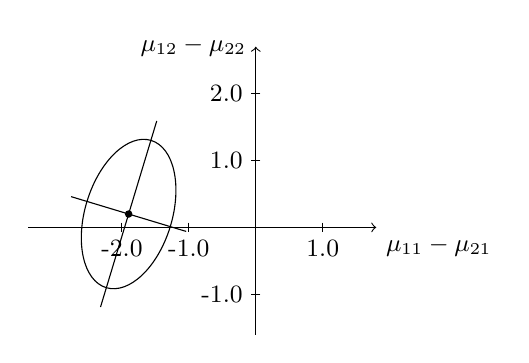
\begin{tikzpicture}[scale=0.85,every node/.style={font=\small}]
% 坐标轴
\draw[->] (-3.4,0)--(1.8,0) node[below right] {$\mu_{11}-\mu_{21}$};
\draw[->] (0,-1.6)--(0,2.7) node[left] {$\mu_{12}-\mu_{22}$};
% 刻度
\foreach \x/\lab in {-2.0/-2.0,-1.0/-1.0,1.0/1.0} {
  \draw (\x,0.07)--(\x,-0.07);
  \node[below] at (\x,-0.05) {\lab};
}
\foreach \y/\lab in {-1.0/-1.0,1.0/1.0,2.0/2.0} {
  \draw (0.07,\y)--(-0.07,\y);
  \node[left] at (-0.05,\y) {\lab};
}
% 95% 置信椭圆
\draw[rotate around={73:(-1.9,0.2)}] (-1.9,0.2) ellipse ({1.15} and {0.65});
% 主轴方向
\draw (-2.32,-1.19)--(-1.48,1.59);
\draw (-2.76,0.46)--(-1.04,-0.06);
\fill (-1.9,0.2) circle (1.6pt);
\end{tikzpicture}
\phantomsection\label{fig:6.1}\mvcap{图 6.1\quad $\boldsymbol{\mu}_1-\boldsymbol{\mu}_2$ 的 95\% 置信椭圆}
\end{mvfigure}

\subsection{联合置信区间}

有可能推出向量 $\boldsymbol{\mu}_1-\boldsymbol{\mu}_2$ 诸分量的联合置信区间，只要考虑诸均值向量之差的所有可能的线性组合即可. 假定各个多元母总体均服从多元正态分布，且具有公共的协方差矩阵 $\boldsymbol{\Sigma}$.

\mvthm{结论 6.3}{设 $c^2=[(n_1+n_2-2)p/(n_1+n_2-p-1)]F_{p,n_1+n_2-p-1}(\alpha)$. 此时对任意的 $\boldsymbol{a}$，
\[
\boldsymbol{a}'(\bar{\mathbf{X}}_1-\bar{\mathbf{X}}_2)\pm c\sqrt{\boldsymbol{a}'\left(\frac{1}{n_1}+\frac{1}{n_2}\right)\mathbf{S}_p\boldsymbol{a}}
\]
将以概率 $1-\alpha$ 包含 $\boldsymbol{a}'(\boldsymbol{\mu}_1-\boldsymbol{\mu}_2)$. 特别是
\[
(\bar{X}_{1i}-\bar{X}_{2i})\pm c\sqrt{\left(\frac{1}{n_1}+\frac{1}{n_2}\right)s_{ii,\mathrm{p}}},\quad i=1,2,\cdots,p
\]
将包含 $\mu_{1i}-\mu_{2i}$.}

\mvbold{证明}\quad 考虑由观测值 $X_{11},X_{12},\cdots,X_{1n_1}$ 与 $X_{21},X_{22},\cdots,X_{2n_2}$ 构成的一元线性组合
\[
\boldsymbol{a}'\mathbf{X}_{1j}=a_1X_{1j1}+a_2X_{1j2}+\cdots+a_pX_{1jp}\qquad 及\qquad \boldsymbol{a}'\mathbf{X}_{2j}=a_1X_{2j1}+a_2X_{2j2}+\cdots+a_pX_{2jp}
\]
这些线性组合的样本均值与样本方差分别为 $\boldsymbol{a}'\bar{\mathbf{X}}_1$，$\boldsymbol{a}'\mathbf{S}_1\boldsymbol{a}$ 及 $\boldsymbol{a}'\bar{\mathbf{X}}_2$，$\boldsymbol{a}'\mathbf{S}_2\boldsymbol{a}$，其中 $\bar{\mathbf{X}}_1,\mathbf{S}_1$ 与 $\bar{\mathbf{X}}_2,\mathbf{S}_2$ 分别为原样本的样本均值和样本方差（见结论 3.5）. 当两个母总体具有相同的协方差阵时，$s_{1,a}^2=\boldsymbol{a}'\mathbf{S}_1\boldsymbol{a}$ 与 $s_{2,a}^2=\boldsymbol{a}'\mathbf{S}_2\boldsymbol{a}$ 二者均为线性组合 $\boldsymbol{a}'\mathbf{X}_1$ 与 $\boldsymbol{a}'\mathbf{X}_2$ 的公共总体方差 $\boldsymbol{a}'\boldsymbol{\Sigma}\boldsymbol{a}$ 的估计量. 融合这些估计量，便得
\phantomsection\label{eq:6-25}
\begin{equation}
\begin{aligned}
s_{a,\mathrm{p}}^2&=\frac{(n_1-1)s_{1,a}^2+(n_2-1)s_{2,a}^2}{(n_1+n_2-2)}\\
&=\boldsymbol{a}'\left[\frac{n_1-1}{n_1+n_2-2}\mathbf{S}_1+\frac{n_2-1}{n_1+n_2-2}\mathbf{S}_2\right]\boldsymbol{a}\\
&=\boldsymbol{a}'\mathbf{S}_p\boldsymbol{a}
\end{aligned}
\tag{6-25}
\end{equation}
为了根据 $\boldsymbol{a}'\mathbf{X}_{1j}$ 和 $\boldsymbol{a}'\mathbf{X}_{2j}$ 检验 $H_0: \boldsymbol{a}'(\boldsymbol{\mu}_1-\boldsymbol{\mu}_2)=\boldsymbol{a}'\boldsymbol{\delta}_0$，我们构造一元二样本 $t$ 统计量的平方
\phantomsection\label{eq:6-26}
\begin{equation}
t_a^2=\frac{[\boldsymbol{a}'(\bar{\mathbf{X}}_1-\bar{\mathbf{X}}_2)-\boldsymbol{a}'(\boldsymbol{\mu}_1-\boldsymbol{\mu}_2)]^2}{\left(\frac{1}{n_1}+\frac{1}{n_2}\right)s_{a,\mathrm{p}}^2}=\frac{[\boldsymbol{a}'(\bar{\mathbf{X}}_1-\bar{\mathbf{X}}_2-(\boldsymbol{\mu}_1-\boldsymbol{\mu}_2))]^2}{\boldsymbol{a}'\left(\frac{1}{n_1}+\frac{1}{n_2}\right)\mathbf{S}_p\boldsymbol{a}}
\tag{6-26}
\end{equation}
根据\hyperref[eq:2-50]{式(2-50)}中的最大化引理，其中 $\boldsymbol{d}=(\bar{\mathbf{X}}_1-\bar{\mathbf{X}}_2-(\boldsymbol{\mu}_1-\boldsymbol{\mu}_2))$ 和 $\mathbf{B}=(1/n_1+1/n_2)\mathbf{S}_p$，我们有，对一切 $\boldsymbol{a}\neq\mathbf{0}$
\[
\begin{aligned}
t_a^2&\leqslant (\bar{\mathbf{X}}_1-\bar{\mathbf{X}}_2-(\boldsymbol{\mu}_1-\boldsymbol{\mu}_2))'\left[\left(\frac{1}{n_1}+\frac{1}{n_2}\right)\mathbf{S}_p\right]^{-1}(\bar{\mathbf{X}}_1-\bar{\mathbf{X}}_2-(\boldsymbol{\mu}_1-\boldsymbol{\mu}_2))\\
&=T^2
\end{aligned}
\]

%% ===== pg-233 =====

% ---- pg-233 （书页 221） ----
因此，
\[
\begin{aligned}
(1-\alpha)&=P[T^2\leqslant c^2]=P[t_a^2\leqslant c^2,\text{对一切 }\boldsymbol{a}]\\
&=P\left[|\boldsymbol{a}'(\bar{\mathbf{X}}_1-\bar{\mathbf{X}}_2)-\boldsymbol{a}'(\boldsymbol{\mu}_1-\boldsymbol{\mu}_2)|\leqslant c\sqrt{\boldsymbol{a}'\left(\frac{1}{n_1}+\frac{1}{n_2}\right)\mathbf{S}_p\boldsymbol{a}},\text{对一切 }\boldsymbol{a}\right]
\end{aligned}
\]
这里的 $c^2$ 根据结论 6.2 选出.\hfill$\blacksquare$

\noindent\textbf{评注}\quad 对检验 $H_0: \boldsymbol{\mu}_1-\boldsymbol{\mu}_2=\mathbf{0}$ 来说，含系数向量 $\hat{\boldsymbol{a}}\propto\mathbf{S}_p^{-1}(\bar{\mathbf{x}}_1-\bar{\mathbf{x}}_2)$ 的线性组合 $\hat{\boldsymbol{a}}'(\bar{\mathbf{x}}_1-\bar{\mathbf{x}}_2)$ 给出了最大总体差值的定量表示. 也就是说，当 $T^2$ 拒绝 $H_0$ 时，$\hat{\boldsymbol{a}}'(\bar{\mathbf{x}}_1-\bar{\mathbf{x}}_2)$ 可能有非零均值. 由于题材和统计上的重要性，我们往往要对这个线性组合的诸分量作出解释.

\noindent\textbf{例 6.4}\quad (计算均值分量之差的联合置信区间)

考虑威斯康星州分别由有空调设备和无空调设备住宅房主构成的两个样本（数据经威斯康星大学统计实验室许可使用）. 样本容量分别为 $n_1=45$ 和 $n_2=55$. 考虑两个用电量测量值（千瓦时），一个是 7 月份用电高峰时的总用电量（$X_1$），另一个是 7 月份非高峰用电时间的用电量（$X_2$）. 其统计结果如下：
\[
\bar{\mathbf{x}}_1=\begin{bmatrix}204.4\\556.6\end{bmatrix},\qquad
\mathbf{S}_1=\begin{bmatrix}13\,825.3&23\,823.4\\23\,823.4&73\,107.4\end{bmatrix},\qquad n_1=45
\]
\[
\bar{\mathbf{x}}_2=\begin{bmatrix}130.0\\355.0\end{bmatrix},\qquad
\mathbf{S}_2=\begin{bmatrix}8\,632.0&19\,616.7\\19\,616.7&55\,964.5\end{bmatrix},\qquad n_2=55
\]
（非高峰时间的耗电量高于高峰时间的耗电量的原因是，在一个月内非高峰用电时间比高峰用电时间长.）

我们来求均值分量之差的 95\% 联合置信区间.

尽管样本方差间存在某些差异，但为明确我们的目的，我们仍用融合的样本协方差阵，此处
\[
\mathbf{S}_\mathrm{p}=\frac{n_1-1}{n_1+n_2-2}\mathbf{S}_1+\frac{n_2-1}{n_1+n_2-2}\mathbf{S}_2=\begin{bmatrix}10\,963.7&21\,505.5\\21\,505.5&63\,661.3\end{bmatrix}
\]
且
\[
\begin{aligned}
c^2&=\frac{(n_1+n_2-2)p}{n_1+n_2-p-1}F_{p,n_1+n_2-p-1}(\alpha)=\frac{98\times 2}{97}\times F_{2,97}(0.05)\\
&=2.02\times 3.1=6.26
\end{aligned}
\]
对 $\boldsymbol{\mu}_1'-\boldsymbol{\mu}_2'=[\mu_{11}-\mu_{21},\mu_{12}-\mu_{22}]$，其总体均值差的 95\% 联合置信区间为：
\[
\mu_{11}-\mu_{21}:\ (204.4-130.0)\pm\sqrt{6.26}\times\sqrt{\left(\frac{1}{45}+\frac{1}{55}\right)\times 10\,963.7}
\]
即
\[
21.7\leqslant\mu_{11}-\mu_{21}\leqslant 127.1
\]
\[
\mu_{12}-\mu_{22}:\ (556.6-355.0)\pm\sqrt{6.26}\times\sqrt{\left(\frac{1}{45}+\frac{1}{55}\right)\times 63\,661.3}
\]
即
\[
74.7\leqslant\mu_{12}-\mu_{22}\leqslant 328.5
\]
于是我们得出结论：有空调设备与无空调设备的家庭的耗电量之间有显著差异，这种差异在用电高峰时间及非高峰时间均存在.

$\boldsymbol{\mu}_1-\boldsymbol{\mu}_2$ 的 95\% 置信椭圆可用其特征值和特征向量确定，其中特征值与特征向量分别为 $\lambda_1=71\,323.5$，$\mathbf{e}_1'=[0.336,0.942]$ 及 $\lambda_2=3\,301.5$，$\mathbf{e}_2'=[0.942,-0.336]$，由于
\[
\sqrt{\lambda_1}\sqrt{\left(\frac{1}{n_1}+\frac{1}{n_2}\right)c^2}=\sqrt{71\,323.5}\times\sqrt{\left(\frac{1}{45}+\frac{1}{55}\right)\times 6.26}=134.3
\]

%% ===== pg-234 =====

% ---- pg-234 （书页 222） ----
\[
\sqrt{\lambda_2}\sqrt{\left(\frac{1}{n_1}+\frac{1}{n_2}\right)c^2}=\sqrt{3\,301.5}\times\sqrt{\left(\frac{1}{45}+\frac{1}{55}\right)\times 6.26}=28.9
\]

\begin{mvfigure}
\centering
\begin{tikzpicture}[scale=0.95,every node/.style={font=\small}]
% 坐标轴
\draw[->] (0,0)--(4.3,0) node[below right] {$\mu_{11}-\mu_{21}$};
\draw[->] (0,0)--(0,4.3) node[left] {$\mu_{12}-\mu_{22}$};
\node[below left] at (0,0) {0};
% 刻度
\foreach \x/\lab in {1.538/100,3.077/200} {
  \draw (\x,0.06)--(\x,-0.06);
  \node[below] at (\x,-0.04) {\lab};
}
\foreach \y/\lab in {1.143/100,2.286/200,3.429/300} {
  \draw (0.06,\y)--(-0.06,\y);
  \node[left] at (-0.05,\y) {\lab};
}
% 95% 置信椭圆
\draw[rotate around={64.3:(1.144,2.304)}] (1.144,2.304) ellipse ({1.604} and {0.433});
% 主轴方向
\draw (0.387,0.726)--(1.901,3.882);
\draw (0.612,2.163)--(1.676,2.445);
\fill (1.144,2.304) circle (1.6pt);
\end{tikzpicture}
\phantomsection\label{fig:6.2}\mvcap{图 6.2\quad $\boldsymbol{\mu}_1'-\boldsymbol{\mu}_2'=(\mu_{11}-\mu_{21},\mu_{12}-\mu_{22})$ 的 95\% 置信椭圆}
\end{mvfigure}

我们得出如\hyperref[fig:6.2]{图 6.2} 所示的 $\boldsymbol{\mu}_1-\boldsymbol{\mu}_2$ 的 95\% 置信椭圆，因为这个均值差的置信椭圆不包含 $\mathbf{0}'=[0,0]$，故在 5\% 显著性水平下，$T^2$ 统计量将拒绝假设 $H_0: \boldsymbol{\mu}_1-\boldsymbol{\mu}_2=\mathbf{0}$.

对拒绝该假设起主要作用的线性组合而言，其系数向量与 $\mathbf{S}_p^{-1}(\bar{\mathbf{x}}_1-\bar{\mathbf{x}}_2)$ 成正比（见练习 6.7）.\hfill$\blacksquare$

$p$ 维总体均值差的 $100(1-\alpha)\%$ \mvbold{庞弗罗尼}联合置信区间为
\[
\mu_{1i}-\mu_{2i}:\ (\bar{x}_{1i}-\bar{x}_{2i})\pm t_{n_1+n_2-2}\left(\frac{\alpha}{2p}\right)\sqrt{\left(\frac{1}{n_1}+\frac{1}{n_2}\right)s_{ii,\mathrm{p}}}
\]
其中的 $t_{n_1+n_2-2}(\alpha/2p)$ 为自由度为 $n_1+n_2-2$ 的 $t$ 分布的上 $100(\alpha/2p)$ 百分位数.

\subsection{\texorpdfstring{$\boldsymbol{\Sigma}_1\neq\boldsymbol{\Sigma}_2$}{Sigma1!=Sigma2} 时的二样本问题}

$\boldsymbol{\Sigma}_1\neq\boldsymbol{\Sigma}_2$ 时，我们无法找到像 $T^2$ 这样的“距离”测度，$T^2$ 的分布与未知的 $\boldsymbol{\Sigma}_1$ 和 $\boldsymbol{\Sigma}_2$ 无关. 虽然我们可用巴特利特检验（见文献[3]）以广义方差的形式来检验 $\boldsymbol{\Sigma}_1$ 与 $\boldsymbol{\Sigma}_2$ 的相等性，不幸的是，当总体为非正态总体时，结论将受到严重误导. 在巴特利特检验中，非正态性与不相等协方差不能分离（参见 6.6 节）. 蒂库和巴拉克里莎（见文献[23]）提出了一种检验两个协方差阵是否相等的方法，该方法对多元正态性假定不太敏感. 不过在我们无条件地介绍这一方法之前，尚需积累更多的实际经验.

我们认为（没有多少实际根据），阶的歧异可能很严重（$\sigma_{1,ii}=4\sigma_{2,ii}$，反过来也一样）. 这在一元情形的确是对的. 在多元情形下，极其重要的歧异大小在很大程度上依赖于变量数目 $p$.

当边际方差之间有较大差异时，某种变换也许能使情况得到改善. 不过当 $n_1$ 与 $n_2$ 很大时，由不相等的协方差阵所引起的复杂性可以避免.

\mvthm{结论 6.4}{设样本容量使 $n_1-p$ 与 $n_2-p$ 都很大，此时 $\boldsymbol{\mu}_1-\boldsymbol{\mu}_2$ 的近似 $100(1-\alpha)\%$ 置信椭球为满足
\[
[\bar{\mathbf{x}}_1-\bar{\mathbf{x}}_2-(\boldsymbol{\mu}_1-\boldsymbol{\mu}_2)]'\left[\frac{1}{n_1}\mathbf{S}_1+\frac{1}{n_2}\mathbf{S}_2\right]^{-1}[\bar{\mathbf{x}}_1-\bar{\mathbf{x}}_2-(\boldsymbol{\mu}_1-\boldsymbol{\mu}_2)]\leqslant\chi_p^2(\alpha)
\]
的所有 $\boldsymbol{\mu}_1-\boldsymbol{\mu}_2$ 给出，其中 $\chi_p^2(\alpha)$ 为自由度为 $p$ 的 $\chi^2$ 分布的上 $100\alpha$ 百分位数. 而且，所有线性组合 $\boldsymbol{a}'(\boldsymbol{\mu}_1-\boldsymbol{\mu}_2)$ 的 $100(1-\alpha)\%$ 联合置信区间为
\[
\boldsymbol{a}'(\bar{\mathbf{x}}_1-\bar{\mathbf{x}}_2)\pm\sqrt{\chi_p^2(\alpha)}\sqrt{\boldsymbol{a}'\left(\frac{1}{n_1}\mathbf{S}_1+\frac{1}{n_2}\mathbf{S}_2\right)\boldsymbol{a}}
\]}

\mvbold{证明}\quad 由\hyperref[eq:6-22]{式(6-22)}及\hyperref[eq:3-9]{式(3-9)}知
\[
E(\bar{\mathbf{X}}_1-\bar{\mathbf{X}}_2)=\boldsymbol{\mu}_1-\boldsymbol{\mu}_2
\]
\[
\operatorname{Cov}(\bar{\mathbf{X}}_1-\bar{\mathbf{X}}_2)=\operatorname{Cov}(\bar{\mathbf{X}}_1)+\operatorname{Cov}(\bar{\mathbf{X}}_2)=\frac{1}{n_1}\boldsymbol{\Sigma}_1+\frac{1}{n_2}\boldsymbol{\Sigma}_2
\]
根据由中心极限定理，$\bar{\mathbf{X}}_1-\bar{\mathbf{X}}_2$ 近似服从 $N_p\left[\boldsymbol{\mu}_1-\boldsymbol{\mu}_2,n_1^{-1}\boldsymbol{\Sigma}_1+n_2^{-1}\boldsymbol{\Sigma}_2\right]$. 若 $\boldsymbol{\Sigma}_1$ 和 $\boldsymbol{\Sigma}_2$ 已知，从 $\bar{\mathbf{X}}_1-\bar{\mathbf{X}}_2$ 到 $\boldsymbol{\mu}_1-\boldsymbol{\mu}_2$ 的统计距离的平方为
\[
[\bar{\mathbf{X}}_1-\bar{\mathbf{X}}_2-(\boldsymbol{\mu}_1-\boldsymbol{\mu}_2)]'\left(\frac{1}{n_1}\boldsymbol{\Sigma}_1+\frac{1}{n_2}\boldsymbol{\Sigma}_2\right)^{-1}[\bar{\mathbf{X}}_1-\bar{\mathbf{X}}_2-(\boldsymbol{\mu}_1-\boldsymbol{\mu}_2)]
\]

%% ===== pg-235 =====

根据结论 4.7，此距离平方近似服从 $\chi_p^2$ 分布. 当 $n_1,n_2$ 很大时，$\mathbf{S}_1$ 和 $\mathbf{S}_2$ 将分别以较大的概率接近 $\boldsymbol{\Sigma}_1$ 和 $\boldsymbol{\Sigma}_2$. 因此，用 $\mathbf{S}_1$ 与 $\mathbf{S}_2$ 分别替换 $\boldsymbol{\Sigma}_1$ 与 $\boldsymbol{\Sigma}_2$ 时近似成立.

关于联合置信区间的结论可从结论 5A.1 得出. \hfill$\blacksquare$

\mvbold{评注}\quad 若 $n_1=n_2=n$，则 $(n-1)/(n+n-2)=1/2$，从而
\begin{align*}
\frac{1}{n_1}\mathbf{S}_1+\frac{1}{n_2}\mathbf{S}_2&=\frac{1}{n}(\mathbf{S}_1+\mathbf{S}_2)=\frac{(n-1)\mathbf{S}_1+(n-1)\mathbf{S}_2}{n+n-2}\left(\frac{1}{n}+\frac{1}{n}\right)\\
&=\mathbf{S}_p\left(\frac{1}{n}+\frac{1}{n}\right)
\end{align*}

故当两个样本的容量相等时，大样本方法和基于融合协方差阵的方法相同（见结论 6.2）. 在一维情形下众所周知：当 $n_1=n_2$ 时，方差不等的效应最小，而当 $n_1\ll n_2$（或 $n_2\ll n_1$）时，方差不等的效应最大.

\noindent\textbf{例 6.5}\quad （推断均值差的大样本方法）

我们用大样本方法来分析例 6.4 中的电力消费数据. 首先计算
\[
\frac{1}{n_1}\mathbf{S}_1+\frac{1}{n_2}\mathbf{S}_2=\frac{1}{45}\times\begin{bmatrix}13\,825.3&23\,823.4\\23\,823.4&73\,107.4\end{bmatrix}+\frac{1}{55}\times\begin{bmatrix}8\,632.0&19\,616.7\\19\,616.7&55\,964.5\end{bmatrix}=\begin{bmatrix}464.17&886.08\\886.08&2\,642.15\end{bmatrix}
\]

线性组合
\[
\mathbf{a}'(\boldsymbol{\mu}_1-\boldsymbol{\mu}_2)=\begin{bmatrix}1,0\end{bmatrix}\begin{bmatrix}\mu_{11}-\mu_{21}\\\mu_{12}-\mu_{22}\end{bmatrix}=\mu_{11}-\mu_{21}
\]
和
\[
\mathbf{a}'(\boldsymbol{\mu}_1-\boldsymbol{\mu}_2)=\begin{bmatrix}0,1\end{bmatrix}\begin{bmatrix}\mu_{11}-\mu_{21}\\\mu_{12}-\mu_{22}\end{bmatrix}=\mu_{12}-\mu_{22}
\]
的 95\% 联合置信区间为（见结论 6.4）：
\begin{align*}
\mu_{11}-\mu_{21}&: 74.4\pm\sqrt{5.99}\sqrt{464.17}\quad 即\quad (21.7,127.1)\\
\mu_{12}-\mu_{22}&: 201.6\pm\sqrt{5.99}\sqrt{2\,642.15}\quad 即\quad (75.8,327.4)
\end{align*}

注意，这些区间与用融合方法处理所得的区间之间的差异是极其微小的. 检验 $H_0: \boldsymbol{\mu}_1-\boldsymbol{\mu}_2=\mathbf{0}$ 的 $T^2$ 检验统计量为
\begin{align*}
T^2&=\begin{bmatrix}\bar{\mathbf{x}}_1-\bar{\mathbf{x}}_2\end{bmatrix}'\left[\frac{1}{n_1}\mathbf{S}_1+\frac{1}{n_2}\mathbf{S}_2\right]^{-1}\begin{bmatrix}\bar{\mathbf{x}}_1-\bar{\mathbf{x}}_2\end{bmatrix}\\
&=\begin{bmatrix}204.4-130.0\\556.6-355.0\end{bmatrix}'\begin{bmatrix}464.17&886.08\\886.08&2\,642.15\end{bmatrix}^{-1}\begin{bmatrix}204.4-130.0\\556.6-355.0\end{bmatrix}\\
&=\begin{bmatrix}74.4&201.6\end{bmatrix}\times 10^{-4}\times\begin{bmatrix}59.874&-20.080\\-20.080&10.519\end{bmatrix}\begin{bmatrix}74.4\\201.6\end{bmatrix}=15.66
\end{align*}

对 $\alpha=0.05$，临界值 $\chi_2^2(0.05)=5.99$. 故由于 $T^2=15.66>\chi_2^2(0.05)=5.99$，我们拒绝 $H_0$. 导致拒绝 $H_0$ 的最关键的线性组合其系数向量为
\begin{align*}
\hat{\mathbf{a}}&\propto\left(\frac{1}{n_1}\mathbf{S}_1+\frac{1}{n_2}\mathbf{S}_2\right)^{-1}(\bar{\mathbf{x}}_1-\bar{\mathbf{x}}_2)=(10^{-4})\begin{bmatrix}59.874&-20.080\\-20.080&10.519\end{bmatrix}\begin{bmatrix}74.4\\201.6\end{bmatrix}\\
&=\begin{bmatrix}0.041\\0.063\end{bmatrix}
\end{align*}

有空调与无空调家庭的非高峰电力消费之差，比高峰电力消费之差对拒绝 $H_0: \boldsymbol{\mu}_1-\boldsymbol{\mu}_2=\mathbf{0}$

%% ===== pg-236 =====

作出的贡献更大. \hfill$\blacksquare$

对小样本及中等大小的样本，蒂库和辛格（见文献[24]）给出了一个类似于 $T^2$ 的统计量，该统计量对离群观测值不太敏感，但是对容量在中等以上的样本，对正态性的微小偏离或存在少数几个离群值就不会对霍特林 $T^2$ 产生明显影响.

\mvsub{当样本容量不大时对正态总体的 $T^2$ 分布的一个近似}

即便两个样本的容量都不大，当总体的协方差矩阵不相等时，我们仍然可以检验 $H_0: \boldsymbol{\mu}_1-\boldsymbol{\mu}_2=\mathbf{0}$，只要这两个总体均是多维正态的. 这种问题经常被称为多变量 Behrens-Fisher 问题. 结果要求两个样本规模 $n_1$ 和 $n_2$ 都要比变量数目 $p$ 大. 这个方法依赖于下述统计量的渐近分布.
\phantomsection\label{eq:6-27}
\begin{equation}
T^2=(\bar{\mathbf{X}}_1-\bar{\mathbf{X}}_2-(\boldsymbol{\mu}_1-\boldsymbol{\mu}_2))'\left[\frac{1}{n_1}\mathbf{S}_1+\frac{1}{n_2}\mathbf{S}_2\right]^{-1}(\bar{\mathbf{X}}_1-\bar{\mathbf{X}}_2-(\boldsymbol{\mu}_1-\boldsymbol{\mu}_2)) \tag{6-27}
\end{equation}
这个式子和结论 6.4 中的大样本统计是一样的. 然而，对于较小的样本（见文献[15]和[19]），建议采用\hyperref[eq:6-28]{式(6-28)}给出的近似逼近，而不是用 $\chi^2$ 近似来求得用来检验 $H_0$ 的临界值.
\phantomsection\label{eq:6-28}
\begin{equation}
T^2=\frac{vp}{v-p+1}F_{p,v-p+1} \tag{6-28}
\end{equation}
在\hyperref[eq:6-28]{式(6-28)}中，自由度 $v$ 是从样本协方差矩阵用\hyperref[eq:6-29]{式(6-29)}估计得到的.
\phantomsection\label{eq:6-29}
\begin{equation}
v=\frac{p+p^2}{\sum\limits_{i=1}^2\frac{1}{n_i}\left\{\left[\mathrm{tr}\left(\frac{1}{n_i}\mathbf{S}_i\left(\frac{1}{n_1}\mathbf{S}_1+\frac{1}{n_2}\mathbf{S}_2\right)^{-1}\right)^2\right]+\left[\mathrm{tr}\left(\frac{1}{n_i}\mathbf{S}_i\left(\frac{1}{n_1}\mathbf{S}_1+\frac{1}{n_2}\mathbf{S}_2\right)^{-1}\right)\right]^2\right\}} \tag{6-29}
\end{equation}
这里 $\min(n_1,n_2)\leqslant v\leqslant n_1+n_2$. 在单变量情形（$p=1$），这个近似就是 Behrens-Fisher 问题通常的 Welch 解.

对中等规模的样本容量和两正态总体，如果
\[
(\bar{\mathbf{x}}_1-\bar{\mathbf{x}}_2-(\boldsymbol{\mu}_1-\boldsymbol{\mu}_2))'\left[\frac{1}{n_1}\mathbf{S}_1+\frac{1}{n_2}\mathbf{S}_2\right]^{-1}(\bar{\mathbf{x}}_1-\bar{\mathbf{x}}_2-(\boldsymbol{\mu}_1-\boldsymbol{\mu}_2))>\frac{vp}{v-p+1}F_{p,v-p+1}(\alpha)
\]
则在近似水平 $\alpha$ 下，拒绝均值相等假设 $H_0: \boldsymbol{\mu}_1-\boldsymbol{\mu}_2=\mathbf{0}$. 上式中，自由度 $v$ 由\hyperref[eq:6-29]{式(6-29)}给出. 除了临界值 $\chi_p^2(\alpha)$ 被较大的常数 $\frac{vp}{v-p+1}F_{p,v-p+1}(\alpha)$ 取代外，这个过程和结论 6.4 中的大样本检验过程是一致的.

类似的，近似的 $100(1-\alpha)\%$ 置信区域由所有的满足下式的 $\boldsymbol{\mu}_1-\boldsymbol{\mu}_2$ 给出.
\phantomsection\label{eq:6-30}
\begin{equation}
(\bar{\mathbf{x}}_1-\bar{\mathbf{x}}_2-(\boldsymbol{\mu}_1-\boldsymbol{\mu}_2))'\left[\frac{1}{n_1}\mathbf{S}_1+\frac{1}{n_2}\mathbf{S}_2\right]^{-1}(\bar{\mathbf{x}}_1-\bar{\mathbf{x}}_2-(\boldsymbol{\mu}_1-\boldsymbol{\mu}_2))\leqslant\frac{vp}{v-p+1}F_{p,v-p+1}(\alpha) \tag{6-30}
\end{equation}

对于正态的总体，由\hyperref[eq:6-28]{式(6-28)}和\hyperref[eq:6-29]{式(6-29)}给出的 $T^2$ 分布近似往往得出合理的结果.

\noindent\textbf{例 6.6}\quad （当 $\boldsymbol{\Sigma}_1\neq\boldsymbol{\Sigma}_2$ 时的 $T^2$ 分布近似）

尽管在例 6.4 中耗电量数据的样本容量相当大，我们用这些数据和例 6.5 中的计算结果来表明这些计算可以得到一个总体协方差矩阵不相等时的近似 $T^2$ 分布.

首先，计算
\[
\frac{1}{n_1}\mathbf{S}_1=\frac{1}{45}\begin{bmatrix}13\,825.2&23\,823.4\\23\,823.4&73\,107.4\end{bmatrix}=\begin{bmatrix}307.227&529.409\\529.409&1\,624.609\end{bmatrix}
\]
\[
\frac{1}{n_2}\mathbf{S}_2=\frac{1}{55}\begin{bmatrix}8\,632.0&19\,616.7\\19\,616.7&55\,964.5\end{bmatrix}=\begin{bmatrix}156.945&356.667\\356.667&1\,017.536\end{bmatrix}
\]

%% ===== pg-237 =====

利用例 6.5 的结论知
\[
\left[\frac{1}{n_1}\mathbf{S}_1+\frac{1}{n_2}\mathbf{S}_2\right]^{-1}=(10^{-4})\begin{bmatrix}59.874&-20.080\\-20.080&10.519\end{bmatrix}
\]
故
\begin{align*}
\frac{1}{n_1}\mathbf{S}_1\left[\frac{1}{n_1}\mathbf{S}_1+\frac{1}{n_2}\mathbf{S}_2\right]^{-1}&=\begin{bmatrix}307.227&529.409\\529.409&1\,624.609\end{bmatrix}(10^{-4})\begin{bmatrix}59.874&-20.080\\-20.080&10.519\end{bmatrix}\\
&=\begin{bmatrix}0.776&-0.060\\-0.092&0.646\end{bmatrix}
\end{align*}
且
\begin{align*}
\left(\frac{1}{n_1}\mathbf{S}_1\left[\frac{1}{n_1}\mathbf{S}_1+\frac{1}{n_2}\mathbf{S}_2\right]^{-1}\right)^2&=\begin{bmatrix}0.776&-0.060\\-0.092&0.646\end{bmatrix}\begin{bmatrix}0.776&-0.060\\-0.092&0.646\end{bmatrix}\\
&=\begin{bmatrix}0.608&-0.085\\-0.131&0.423\end{bmatrix}
\end{align*}
进一步，有
\begin{align*}
\frac{1}{n_2}\mathbf{S}_2\left[\frac{1}{n_1}\mathbf{S}_1+\frac{1}{n_2}\mathbf{S}_2\right]^{-1}&=\begin{bmatrix}156.945&356.667\\356.667&1\,017.536\end{bmatrix}(10^{-4})\begin{bmatrix}59.874&-20.080\\-20.080&10.519\end{bmatrix}\\
&=\begin{bmatrix}0.224&-0.060\\-0.092^{\ast}&0.354\end{bmatrix}
\end{align*}
和
\begin{align*}
\left(\frac{1}{n_2}\mathbf{S}_2\left[\frac{1}{n_1}\mathbf{S}_1+\frac{1}{n_2}\mathbf{S}_2\right]^{-1}\right)^2&=\begin{bmatrix}0.224&-0.060\\-0.092&0.354\end{bmatrix}\begin{bmatrix}0.224&-0.060\\-0.092&0.354\end{bmatrix}\\
&=\begin{bmatrix}0.055&0.035\\0.053&0.131\end{bmatrix}
\end{align*}
于是，
\begin{align*}
&\frac{1}{n_1}\left\{\mathrm{tr}\left[\left(\frac{1}{n_1}\mathbf{S}_1\left(\frac{1}{n_1}\mathbf{S}_1+\frac{1}{n_2}\mathbf{S}_2\right)^{-1}\right)^2\right]+\left[\mathrm{tr}\left(\frac{1}{n_1}\mathbf{S}_1\left(\frac{1}{n_1}\mathbf{S}_1+\frac{1}{n_2}\mathbf{S}_2\right)^{-1}\right)\right]^2\right\}\\
&\qquad=\frac{1}{45}[(0.608+0.423)+(0.776+0.646)^2]=0.067\,8
\end{align*}
\begin{align*}
&\frac{1}{n_2}\left\{\mathrm{tr}\left[\left(\frac{1}{n_2}\mathbf{S}_2\left(\frac{1}{n_1}\mathbf{S}_1+\frac{1}{n_2}\mathbf{S}_2\right)^{-1}\right)^2\right]+\left[\mathrm{tr}\left(\frac{1}{n_2}\mathbf{S}_2\left(\frac{1}{n_1}\mathbf{S}_1+\frac{1}{n_2}\mathbf{S}_2\right)^{-1}\right)\right]^2\right\}\\
&\qquad=\frac{1}{55}[(0.055+0.131)+(0.224+0.354)^2]=0.009\,5
\end{align*}
利用\hyperref[eq:6-29]{式(6-29)}，自由度 $v$ 为
\[
v=\frac{2+2^2}{0.067\,8+0.009\,5}=77.6
\]
且 $\alpha=0.05$ 时的临界值为
\[
\frac{vp}{v-p+1}F_{p,v-p+1}(0.05)=\frac{77.6\times 2}{77.6-2+1}F_{2,77.6-2+1}(0.05)=\frac{155.2}{76.6}\times 3.12=6.32
\]
从例 6.5，检验统计量的观测值是 $T^2=15.66$，所以在 5\% 水平时，假设 $H_0: \boldsymbol{\mu}_1-\boldsymbol{\mu}_2=\mathbf{0}$ 被拒绝. 这个结论和例 6.5 中大样本过程得到的结论一样. \hfill$\blacksquare$

在例 6.6 中，非整数自由度的 $F_{p,v-p+1}$ 分布也可以定义. 一个稍微保守的近似是采用 $v$ 的整数部分.

\noindent\rule{\linewidth}{0.4pt}

{\small $\ast$ 原著为 0.092，疑有误，更正为 $-0.092$. —— 译者注}

%% ===== pg-238 =====

\section{多个多元总体均值向量的比较（单因子多元方差分析）}  % 原书 6.4
\phantomsection\label{sec:6.4}

我们常常需要对两个以上的总体进行比较. 设从 $g$ 个总体分别抽取的随机样本为
\phantomsection\label{eq:6-31}
\begin{equation}
\begin{array}{l}
\text{总体 } 1\text{：}\quad \mathbf{X}_{11},\mathbf{X}_{12},\cdots,\mathbf{X}_{1n_1}\\
\text{总体 } 2\text{：}\quad \mathbf{X}_{21},\mathbf{X}_{22},\cdots,\mathbf{X}_{2n_2}\\
\qquad\vdots\qquad\qquad\vdots\\
\text{总体 } g\text{：}\quad \mathbf{X}_{g1},\mathbf{X}_{g2},\cdots,\mathbf{X}_{gn_g}
\end{array}
\tag{6-31}
\end{equation}
多元方差分析首先被用来研究这些总体的均值向量是否相等，若不等，那么哪些分量有显著差异.

\mvsub{单因子多元方差分析的数据结构假设}

1. 设 $\mathbf{X}_{l1},\mathbf{X}_{l2},\cdots,\mathbf{X}_{ln_l}$ 为来自均值为 $\boldsymbol{\mu}_l$ 的总体的一容量为 $n_l$ 的随机样本，$l=1,2,\cdots,g$. 来自不同总体的样本相互独立.

2. 所有总体均具有公共的协方差矩阵 $\boldsymbol{\Sigma}$.

3. 每个总体均为多元正态总体.

当所有样本容量 $n_l$ 均充分大时，根据中心极限定理（结论 4.13），可将条件 3 放宽.

在开始讨论多元方差分析之前，回顾一下一元方差分析（ANOVA）是有益的.

\mvsub{一元方差分析概述}

在一元情形下的假设为：$X_{l1},X_{l2},\cdots,X_{ln_l}$ 为来自总体 $N(\mu_l,\sigma^2)$，$l=1,2,\cdots,g$ 的随机样本，而且来自不同总体的样本相互独立. 虽然关于均值相等的零假设可陈述为 $\mu_1=\mu_2=\cdots=\mu_g$，但我们习惯于将 $\mu_l$ 表示成总均值分量 $\mu$ 与某个归因于特定总体的分量之和，例如，$\mu_l=\mu+(\mu_l-\mu)$ 或 $\mu_l=\mu+\tau_l$，其中 $\tau_l=\mu_l-\mu$.

不同总体通常对应于不同的实验条件，因此，研究与第 $l$ 个总体（处理）相联系的偏差 $\tau_l$ 是合适的.

重新参数化
\phantomsection\label{eq:6-32}
\begin{equation}
\begin{array}{c@{\ }c@{\ }c@{\ }c@{\ }c}
\mu_l & = & \mu & + & \tau_l\\[2pt]
(\text{第 } l \text{ 个总体} & & (\text{总均} & & (\text{第 } l \text{ 个总体（处理）}\\
\text{均值}) & & \text{值}) & & \text{的效应})
\end{array}
\tag{6-32}
\end{equation}
导致均值相等性假设的另一种表述：
\[
H_0: \tau_1=\tau_2=\cdots=\tau_g=0
\]
而服从分布 $N(\mu+\tau_l,\sigma^2)$ 的响应 $X_{lj}$ 则可表示成如下形式：
\phantomsection\label{eq:6-33}
\begin{equation}
\begin{array}{c@{\ }c@{\ }c@{\ }c@{\ }c@{\ }c@{\ }c}
X_{lj} & = & \mu & + & \tau_l & + & e_{lj}\\
& & (\text{总均值}) & & (\text{处理效应}) & & (\text{随机误差})
\end{array}
\tag{6-33}
\end{equation}
其中 $e_{lj}$ 为独立同分布随机变量，其分布为 $N(0,\sigma^2)$. 为了唯一地确定模型参数及它们的最小二乘估计值，通常需附加约束条件 $\sum\limits_{l=1}^g n_l\tau_l=0$.

受分解\hyperref[eq:6-33]{式(6-33)}的启发，方差分析可在对观测值进行类似分解的基础上进行：
\phantomsection\label{eq:6-34}
\begin{equation}
\begin{array}{c@{\ }c@{\ }c@{\ }c@{\ }c@{\ }c@{\ }c}
x_{lj} & = & \bar{x} & + & (\bar{x}_l-\bar{x}) & + & (x_{lj}-\bar{x}_l)\\
(\text{观测值}) & & (\text{样本总均值}) & & (\text{处理效应的估计}) & & (\text{残差})
\end{array}
\tag{6-34}
\end{equation}

%% ===== pg-239 =====

其中 $\bar{x}$ 为 $\mu$ 的估计，$\hat{\tau}_l=(\bar{x}_l-\bar{x})$ 为 $\tau_l$ 的估计而 $(x_{lj}-\bar{x}_l)$ 为误差 $e_{lj}$ 的估计.

\noindent\textbf{例 6.7}\quad （一元 ANOVA 的平方和分解）

考虑如下独立样本

总体 1：$9,6,9$\\
总体 2：$0,2$\\
总体 3：$3,1,2$

由于，比如说 $x_{31}=(3+1+2)/3=2$ 和 $\bar{x}=(9+6+9+0+2+3+1+2)/8=4$，我们有
\begin{align*}
3&=x_{31}=\bar{x}+(\bar{x}_3-\bar{x})+(x_{31}-\bar{x}_3)\\
&=4+(2-4)+(3-2)\\
&=4+(-2)+1
\end{align*}
对每个观测值作上述的分解，便得
\[
\begin{bmatrix}9&6&9\\0&2&\\3&1&2\end{bmatrix}=\begin{bmatrix}4&4&4\\4&4&\\4&4&4\end{bmatrix}+\begin{bmatrix}4&4&4\\-3&-3&\\-2&-2&-2\end{bmatrix}+\begin{bmatrix}1&-2&1\\-1&1&\\-1&-1&0\end{bmatrix}
\]
\[
\text{观测值}\qquad\text{均值}\qquad\text{处理效应}\qquad\text{残差}
\]
\[
(x_{lj})\qquad(\bar{x})\qquad(\bar{x}_l-\bar{x})\qquad(x_{lj}-\bar{x}_l)
\]
通过评估处理效应的贡献是否比残差的贡献大，就能回答均值的相等性问题.（$\tau_l$ 的估计 $\hat{\tau}_l=\bar{x}_l-\bar{x}$ 总满足 $\sum\limits_{l=1}^g n_l\hat{\tau}_l=0$，在假设 $H_0$ 下，每一个 $\hat{\tau}_l$ 均为 0 的估计.）若处理的贡献很大，应拒绝 $H_0$. 对上述 4 个矩阵，分别求出其所有元素的平方和（SS）. 对这些观测值，我们构造一个向量 $\mathbf{y}'=[9,6,9,0,2,3,1,2]$，其平方和为
\[
\mathrm{SS}_{\text{观测}}=9^2+6^2+9^2+0^2+2^2+3^2+1^2+2^2=216
\]
类似地，有
\[
\mathrm{SS}_{\text{均值}}=4^2+4^2+4^2+4^2+4^2+4^2+4^2+4^2=8\times 4^2=128
\]
\begin{align*}
\mathrm{SS}_{\text{处理}}&=4^2+4^2+4^2+(-3)^2+(-3)^2+(-2)^2+(-2)^2+(-2)^2\\
&=3\times 4^2+2\times(-3)^2+3\times(-2)^2=78
\end{align*}
以及残差平方和
\[
\mathrm{SS}_{\text{残差}}=1^2+(-2)^2+1^2+(-1)^2+1^2+1^2+(-1)^2+0^2=10
\]
这些平方和满足与\hyperref[eq:6-34]{式(6-34)}一样的分解式，故
\[
\mathrm{SS}_{\text{观测}}=\mathrm{SS}_{\text{均值}}+\mathrm{SS}_{\text{处理}}+\mathrm{SS}_{\text{残差}}
\]
即 $216=128+78+10$. 总平方和的这种分解把样本中的总变差分解成来自总均值、处理和残差三部分，方差分析就是要进行 $\mathrm{SS}_{\text{处理}}$ 与 $\mathrm{SS}_{\text{残差}}$ 的大小比较. 假如 $H_0$ 为真，那么由 $\mathrm{SS}_{\text{处理}}$ 与 $\mathrm{SS}_{\text{残差}}$ 算出的变差应近似相等. \hfill$\blacksquare$

在例 6.7 中用数字说明的平方和分解方法是非常基本的，现在来推导这种分解的代数式.

从\hyperref[eq:6-34]{式(6-34)}两边减去 $\bar{x}$，然后取平方，得
\[
(x_{lj}-\bar{x})^2=(\bar{x}_l-\bar{x})^2+(x_{lj}-\bar{x}_l)^2+2(\bar{x}_l-\bar{x})(x_{lj}-\bar{x}_l)
\]
两边对 $j$ 求和，注意到 $\sum\limits_{j=1}^{n_l}(x_{lj}-\bar{x}_l)=0$，就有

%% ===== pg-240 =====

\[
\sum_{j=1}^{n_l}(x_{lj}-\bar{x})^2=n_l(\bar{x}_l-\bar{x})^2+\sum_{j=1}^{n_l}(x_{lj}-\bar{x}_l)^2
\]
然后，两边再对 $l$ 求和，可得
\phantomsection\label{eq:6-35}
\begin{equation}
\mvfit{$\displaystyle
\sum_{l=1}^g\sum_{j=1}^{n_l}(x_{lj}-\bar{x})^2=\sum_{l=1}^g n_l(\bar{x}_l-\bar{x})^2+\sum_{l=1}^g\sum_{j=1}^{n_l}(x_{lj}-\bar{x}_l)^2
$} \tag{6-35}
\end{equation}
\[
\mathrm{SS}_{\text{总}}=\mathrm{SS}_{\text{组间}}+\mathrm{SS}_{\text{组内}}
\]
\[
(\text{总（修正的）平方和})=(\text{组间平方和})+(\text{组内平方和})
\]
即
\phantomsection\label{eq:6-36}
\begin{equation}
\mvfit{$\displaystyle
\sum_{l=1}^g\sum_{j=1}^{n_l}x_{lj}^2=(n_1+n_2+\cdots+n_g)\bar{x}^2+\sum_{l=1}^g n_l(\bar{x}_l-\bar{x})^2+\sum_{l=1}^g\sum_{j=1}^{n_l}(x_{lj}-\bar{x}_l)^2
$} \tag{6-36}
\end{equation}
\[
(\mathrm{SS}_{\text{观测}})=(\mathrm{SS}_{\text{均值}})+(\mathrm{SS}_{\text{处理}})+(\mathrm{SS}_{\text{残差}})
\]

在\hyperref[eq:6-36]{式(6-36)}的推导过程中，我们实际上已证明了均值向量、处理效应向量及残差向量是相互正交的. 也就是说，对任意的观测值向量 $\mathbf{y}'=[x_{11},\cdots,x_{1n_1},x_{21},\cdots,x_{2n_2},\cdots,x_{gn_g}]$，这些数组视作向量的都是正交的. 因此只要利用 $\mathrm{SS}_{\text{残差}}=\mathrm{SS}_{\text{观测}}-\mathrm{SS}_{\text{均值}}-\mathrm{SS}_{\text{处理}}$，不用计算单个残差便得到 $\mathrm{SS}_{\text{残差}}$. 但这种方法并不经济，因为由单个残差构成的残差图实际上可为模型中的假定提供检验.

包含在分解\hyperref[eq:6-34]{式(6-34)}中的数组的向量表示具有能提供自由度的几何解释. 对任一观测值集，令 $\mathbf{y}'=[x_{11},\cdots,x_{1n_1},x_{21},\cdots,x_{2n_2},\cdots,x_{gn_g}]$. 观测值向量 $\mathbf{y}$ 可以在 $n=n_1+n_2+\cdots+n_g$ 维空间的任何地方，均值向量 $\bar{x}\mathbf{1}=[\bar{x},\cdots,\bar{x}]'$ 必定处在 $\mathbf{1}$ 的等角线上，而处理效应向量
\[
(\bar{x}_1-\bar{x})\left.\begin{bmatrix}1\\\vdots\\1\\0\\\vdots\\0\\0\\\vdots\\0\end{bmatrix}\right\}n_1
+(\bar{x}_2-\bar{x})\left.\begin{bmatrix}0\\\vdots\\0\\1\\\vdots\\1\\0\\\vdots\\0\end{bmatrix}\right\}n_2
+\cdots+(\bar{x}_g-\bar{x})\left.\begin{bmatrix}0\\\vdots\\0\\0\\\vdots\\0\\1\\\vdots\\1\end{bmatrix}\right\}n_g
\]
\[
=(\bar{x}_1-\bar{x})\mathbf{u}_1+(\bar{x}_2-\bar{x})\mathbf{u}_2+\cdots+(\bar{x}_g-\bar{x})\mathbf{u}_g
\]
则位于 $g$ 个向量 $\mathbf{u}_1,\mathbf{u}_2,\cdots,\mathbf{u}_g$ 的线性组合所张成的超平面中. 又因 $\mathbf{1}=\mathbf{u}_1+\mathbf{u}_2+\cdots+\mathbf{u}_g$，故均值向量也位于这个超平面中，而且总与处理效应向量垂直（见练习 6.10）. 因此，均值向量可在 1 维空间中变化，而处理效应向量则在一个 $g-1$ 维空间中变化. 残差向量 $\hat{\mathbf{e}}=\mathbf{y}-(\bar{x}\mathbf{1})-[(\bar{x}_1-\bar{x})\mathbf{u}_1+\cdots+(\bar{x}_g-\bar{x})\mathbf{u}_g]$ 与均值向量及处理效应向量均垂直，所以只能在与它们的超平面垂直的 $n-(g-1)-1=n-g$ 维子空间中变化.

概括地说，$\mathrm{SS}_{\text{组间}}$、$\mathrm{SS}_{\text{处理}}$ 和 $\mathrm{SS}_{\text{残差}}$ 的自由度分别为 $1,g-1$ 和 $n-g=(n_1+n_2+\cdots+n_g)-g$. 总自由度为 $n=n_1+n_2+\cdots+n_g$. 另外，根据一元分布理论，我们发现这些自由度正是各平方和所对应的 $\chi^2$ 分布的自由度.

平方和的计算以及相应的自由度可方便地用 ANOVA 表来表示.

%% ===== pg-241 =====

\begin{mvtable}
\mvtabcap{比较一元总体均值的 ANOVA 表}
\begin{tabular}{ccc}
\toprule
变差来源 & 平方和（SS） & 自由度（d.f.）\\
\midrule
处理 & $\mathrm{SS}_{\text{处理}}=\sum\limits_{l=1}^g n_l(\bar{x}_l-\bar{x})^2$ & $g-1$\\
残差（误差） & $\mathrm{SS}_{\text{残差}}=\sum\limits_{l=1}^g\sum\limits_{j=1}^{n_l}(x_{lj}-\bar{x}_l)^2$ & $\sum\limits_{l=1}^g n_l-g$\\
\midrule
总和 & $\mathrm{SS}_{\text{总}}=\sum\limits_{l=1}^g\sum\limits_{j=1}^{n_l}(x_{lj}-\bar{x})^2$ & $\sum\limits_{l=1}^g n_l-1$\\
\bottomrule
\end{tabular}
\end{mvtable}

若 $F=\dfrac{\mathrm{SS}_{\text{处理}}/(g-1)}{\mathrm{SS}_{\text{残差}}\big/\left(\sum\limits_{l=1}^g n_l-g\right)}>F_{g-1,\sum n_l-g}(\alpha)$，则在显著性水平 $\alpha$ 下拒绝 $H_0: \tau_1=\tau_2=\cdots=\tau_g=0$. 此处 $F_{g-1,\sum n_l-g}(\alpha)$ 为自由度为 $g-1$ 和 $\sum\limits_{l=1}^g n_l-g$ 的 $F$ 分布的 $100\alpha$ 百分位数. 这相当于在 $\mathrm{SS}_{\text{处理}}/\mathrm{SS}_{\text{残差}}$ 值很大或 $1+\mathrm{SS}_{\text{处理}}/\mathrm{SS}_{\text{残差}}$ 值很大时拒绝 $H_0$. 适合向多元情形推广的检验统计量为
\phantomsection\label{eq:6-37}
\begin{equation}
\frac{1}{1+\mathrm{SS}_{\text{处理}}/\mathrm{SS}_{\text{残差}}}=\frac{\mathrm{SS}_{\text{残差}}}{\mathrm{SS}_{\text{残差}}+\mathrm{SS}_{\text{处理}}} \tag{6-37}
\end{equation}
当此值很小时，就拒绝 $H_0$.

\noindent\textbf{例 6.8}\quad （一元 ANOVA 表及处理效应的 $F$ 检验）

利用例 6.7 的信息，可得出如下 ANOVA 表：

\begin{mvtable}
\begin{tabular}{ccc}
\toprule
变差来源 & 平方和 & 自由度\\
\midrule
处理 & $\mathrm{SS}_{\text{处理}}=78$ & $g-1=3-1=2$\\
残差 & $\mathrm{SS}_{\text{残差}}=10$ & $\sum\limits_{l=1}^g n_l-g=(3+2+3)-3=5$\\
\midrule
总和 & $\mathrm{SS}_{\text{总}}=88$ & $\sum\limits_{l=1}^g n_l-1=7$\\
\bottomrule
\end{tabular}
\end{mvtable}

于是
\[
F=\frac{\mathrm{SS}_{\text{处理}}/(g-1)}{\mathrm{SS}_{\text{残差}}\big/\left(\sum n_l-g\right)}=\frac{78/2}{10/5}=19.5
\]
由于 $F=19.5>F_{2,5}(0.01)=13.27$，所以在 0.01 显著性水平下，我们拒绝 $H_0: \tau_1=\tau_2=\tau_3=0$（即无处理效应）. \hfill$\blacksquare$

\mvsub{多元方差分析（MANOVA）}

与一元情形的重新参数化类似，我们先建立 MANOVA 模型如下：

\begin{mvframe}[比较 $g$ 个总体均值向量的 MANOVA 模型]
\phantomsection\label{eq:6-38}
\begin{equation}
\mathbf{X}_{lj}=\boldsymbol{\mu}+\boldsymbol{\tau}_l+\mathbf{e}_{lj},\quad j=1,2,\cdots,n_l,\ l=1,2,\cdots,g \tag{6-38}
\end{equation}
此处 $\mathbf{e}_{lj}$ 为独立的 $N_p(\mathbf{0},\boldsymbol{\Sigma})$ 随机变量，参数向量 $\boldsymbol{\mu}$ 为总均值（水平），而 $\boldsymbol{\tau}_l$ 则代表第 $l$ 个处理效应，且满足 $\sum\limits_{l=1}^g n_l\boldsymbol{\tau}_l=\mathbf{0}$.
\end{mvframe}

%% ===== pg-242 =====

根据模型（6-38），观测值向量 $\mathbf{X}_{lj}$ 的每个分量满足一元模型（6-33），但 $\mathbf{X}_{lj}$ 的分量的误差彼此相关，且所有总体的协方差矩阵 $\boldsymbol{\Sigma}$ 均相同.

观测值向量可按模型所暗示的方式分解如下：
\phantomsection\label{eq:6-39}
\begin{equation}
\begin{array}{c@{\ }c@{\ }c@{\ }c@{\ }c@{\ }c@{\ }c}
\mathbf{x}_{lj} & = & \bar{\mathbf{x}} & + & (\bar{\mathbf{x}}_l-\bar{\mathbf{x}}) & + & (\mathbf{x}_{lj}-\bar{\mathbf{x}}_l)\\
(\text{观测值}) & & \left(\begin{array}{c}\text{样本总}\\\text{均值}\hat{\boldsymbol{\mu}}\end{array}\right) & & \left(\begin{array}{c}\text{处理效应}\\\text{的估计}\hat{\boldsymbol{\tau}}_l\end{array}\right) & & \left(\begin{array}{c}\text{残差}\\\hat{\mathbf{e}}_{lj}\end{array}\right)
\end{array}
\tag{6-39}
\end{equation}
分解\hyperref[eq:6-39]{式(6-39)}导致与一元情形相类似的多元平方和分解式. 首先，注意到乘积 $(\mathbf{x}_{lj}-\bar{\mathbf{x}})(\mathbf{x}_{lj}-\bar{\mathbf{x}})'$ 可写成
\begin{align*}
(\mathbf{x}_{lj}-\bar{\mathbf{x}})(\mathbf{x}_{lj}-\bar{\mathbf{x}})'&=[(\mathbf{x}_{lj}-\bar{\mathbf{x}}_l)+(\bar{\mathbf{x}}_l-\bar{\mathbf{x}})][(\mathbf{x}_{lj}-\bar{\mathbf{x}}_l)+(\bar{\mathbf{x}}_l-\bar{\mathbf{x}})]'\\
&=(\mathbf{x}_{lj}-\bar{\mathbf{x}}_l)(\mathbf{x}_{lj}-\bar{\mathbf{x}}_l)'+(\mathbf{x}_{lj}-\bar{\mathbf{x}}_l)(\bar{\mathbf{x}}_l-\bar{\mathbf{x}})'\\
&\qquad+(\bar{\mathbf{x}}_l-\bar{\mathbf{x}})(\mathbf{x}_{lj}-\bar{\mathbf{x}}_l)'+(\bar{\mathbf{x}}_l-\bar{\mathbf{x}})(\bar{\mathbf{x}}_l-\bar{\mathbf{x}})'
\end{align*}
因为 $\sum\limits_{j=1}^{n_l}(\mathbf{x}_{lj}-\bar{\mathbf{x}}_l)=\mathbf{0}$，所以对 $j$ 求和后，中间两项均为零矩阵. 于是将交叉乘积对 $l$ 和 $j$ 求和后可得：
\phantomsection\label{eq:6-40}
\begin{equation}
\sum_{l=1}^g\sum_{j=1}^{n_l}(\mathbf{x}_{lj}-\bar{\mathbf{x}})(\mathbf{x}_{lj}-\bar{\mathbf{x}})'=\sum_{l=1}^g n_l(\bar{\mathbf{x}}_l-\bar{\mathbf{x}})(\bar{\mathbf{x}}_l-\bar{\mathbf{x}})'+\sum_{l=1}^g\sum_{j=1}^{n_l}(\mathbf{x}_{lj}-\bar{\mathbf{x}}_l)(\mathbf{x}_{lj}-\bar{\mathbf{x}}_l)' \tag{6-40}
\end{equation}
\[
\begin{array}{ccc}
\text{（总平方和及交叉乘积和）} & \text{（处理平方和及} & \text{（残差平方和及}\\
& \text{交叉乘积和（或} & \text{交叉乘积和（或}\\
& \text{组间平方和））} & \text{组内平方和））}
\end{array}
\]
组内平方和可表示为
\phantomsection\label{eq:6-41}
\begin{equation}
\begin{aligned}
\mathbf{W}&=\sum_{l=1}^g\sum_{j=1}^{n_l}(\mathbf{x}_{lj}-\bar{\mathbf{x}}_l)(\mathbf{x}_{lj}-\bar{\mathbf{x}}_l)'\\
&=(n_1-1)\mathbf{S}_1+(n_2-1)\mathbf{S}_2+\cdots+(n_g-1)\mathbf{S}_g
\end{aligned}
\tag{6-41}
\end{equation}
其中 $\mathbf{S}_l$ 为第 $l$ 个样本的样本协方差矩阵. 它是二样本时 $(n_1+n_2-2)\mathbf{S}_p$ 的推广，在处理效应的存在性检验中，它起着决定性作用.

同一元情形相似，可通过比较处理与残差的平方和及交叉乘积和的相对大小，来检验关于无处理效应的假设
\[
H_0: \boldsymbol{\tau}_1=\boldsymbol{\tau}_2=\cdots=\boldsymbol{\tau}_g=\mathbf{0}
\]
等价的做法是，也可以考虑残差与总和（修正后）的平方和及交叉乘积和的相对大小. 我们将得出检验统计量的计算用 MANOVA 表列出.

\begin{mvtable}
\mvtabcap{总体均值向量比较的 MANOVA 表}
\begin{tabular}{ccc}
\toprule
变差来源 & 平方和及交叉乘积和矩阵（SSP） & 自由度（d.f.）\\
\midrule
处理 & $\mathbf{B}=\sum\limits_{l=1}^g n_l(\bar{\mathbf{x}}_l-\bar{\mathbf{x}})(\bar{\mathbf{x}}_l-\bar{\mathbf{x}})'$ & $g-1$\\
残差（误差） & $\mathbf{W}=\sum\limits_{l=1}^g\sum\limits_{j=1}^{n_l}(\mathbf{x}_{lj}-\bar{\mathbf{x}}_l)(\mathbf{x}_{lj}-\bar{\mathbf{x}}_l)'$ & $\sum\limits_{l=1}^g n_l-g$\\
\midrule
总和（修正后的） & $\mathbf{B}+\mathbf{W}=\sum\limits_{l=1}^g\sum\limits_{j=1}^{n_l}(\mathbf{x}_{lj}-\bar{\mathbf{x}})(\mathbf{x}_{lj}-\bar{\mathbf{x}})'$ & $\sum\limits_{l=1}^g n_l-1$\\
\bottomrule
\end{tabular}
\end{mvtable}

%% ===== pg-243 =====

此表与一元情形下的 ANOVA 表形式完全相同, 只是 ANOVA 表中标量平方和在此处已被相应的向量分量的平方和所代替. 例如 $(\bar{x}_1-\bar{x})^2$ 被换成了 $(\bar{\mathbf{x}}_1-\bar{\mathbf{x}})(\bar{\mathbf{x}}_1-\bar{\mathbf{x}})'$. 各种自由度与一元几何对应, 因而也与某种包含威沙特密度在内的多元分布原理相对应(见文献[1]).

假设 $H_0:\boldsymbol{\tau}_1=\boldsymbol{\tau}_2=\cdots=\boldsymbol{\tau}_g=\mathbf{0}$ 的一个检验涉及广义方差, 若广义方差比
\phantomsection\label{eq:6-42}
\begin{equation}
\Lambda^*=\frac{|W|}{|B+W|}
=\frac{\left|\sum\limits_{i=1}^{g}\sum\limits_{j=1}^{n_i}(\mathbf{x}_{ij}-\bar{\mathbf{x}}_i)(\mathbf{x}_{ij}-\bar{\mathbf{x}}_i)'\right|}
{\left|\sum\limits_{i=1}^{g}\sum\limits_{j=1}^{n_i}(\mathbf{x}_{ij}-\bar{\mathbf{x}})(\mathbf{x}_{ij}-\bar{\mathbf{x}})'\right|}
\tag{6-42}
\end{equation}
过小, 则拒绝 $H_0$. $\Lambda^*=|W|/|B+W|$ 这个量最早是由威尔克斯提出的(见文献[25]), 它与一元情形下假设“$H_0$: 无处理效应”的 $F$ 检验的等价形\hyperref[eq:6-33]{式(6-33)}相对应. 威尔克斯\footnote{威尔克斯 $\Lambda$ 统计量也可表示成 $W^{-1}B$ 的特征值的函数: $\Lambda^*=\prod\limits_{i=1}^{s}\left(\frac{1}{1+\lambda_i}\right)$, 其中 $s=\min(p,g-1)$ 为 $B$ 的秩. 其他用于检验若干个多元均值向量相等性的检验统计量, 如皮莱曼统计量、劳雷-霍尔特统计量及罗伊最大根统计量, 均可表示为 $W^{-1}B$ 的特征值的函数, 对大样本情形, 这些统计量基本上是等价的(详见后面的讨论).}$\Lambda$ 统计量的优点是使用方便, 而且与似然比准则密切相关. 对于\hyperref[tab:6.3]{表 6.3} 所列的一些特殊情形, 可导出 $\Lambda^*$ 的精确分布. 对于其他情形及大样本情形, 经巴特利特(见文献[4])修正的 $\Lambda^*$ 可用于检验 $H_0$.

\begin{mvtable}
\phantomsection\label{tab:6.3}\mvtabcap{表 6.3\quad 威尔克斯 $\Lambda^*=|W|/|B+W|$ 的分布}
\begin{tabular}{ccc}
\toprule
变量数 & 组数 & 多元正态数据的抽样分布\\
\midrule
$p=1$ & $g\geqslant 2$ & $\left(\dfrac{\sum n_i-g}{g-1}\right)\left(\dfrac{1-\Lambda^*}{\Lambda^*}\right)\sim F_{g-1,\sum n_i-g}$\\[6pt]
$p=2$ & $g\geqslant 2$ & $\left(\dfrac{\sum n_i-g-1}{g-1}\right)\left(\dfrac{1-\sqrt{\Lambda^*}}{\sqrt{\Lambda^*}}\right)\sim F_{2(g-1),2(\sum n_i-g-1)}$\\[6pt]
$p\geqslant 1$ & $g=2$ & $\left(\dfrac{\sum n_i-p-1}{p}\right)\left(\dfrac{1-\Lambda^*}{\Lambda^*}\right)\sim F_{p,\sum n_i-p-1}$\\[6pt]
$p\geqslant 1$ & $g=3$ & $\left(\dfrac{\sum n_i-p-2}{p}\right)\left(\dfrac{1-\sqrt{\Lambda^*}}{\sqrt{\Lambda^*}}\right)\sim F_{2p,2(\sum n_i-p-2)}$\\[6pt]
\bottomrule
\end{tabular}
\end{mvtable}

巴特利特(见文献[4])证明了, 若假设 $H_0$ 为真且 $\sum n_i=n$ 充分大, 则
\phantomsection\label{eq:6-43}
\begin{equation}
-\left(n-1-\frac{(p+g)}{2}\right)\ln\Lambda^*
=-\left(n-1-\frac{(p+g)}{2}\right)\ln\left(\frac{|W|}{|B+W|}\right)
\tag{6-43}
\end{equation}
近似服从自由度为 $p(g-1)$ 的 $\chi^2$ 分布, 因此, 当 $\sum n_i=n$ 充分大时, 若
\phantomsection\label{eq:6-44}
\begin{equation}
-\left(n-1-\frac{(p+g)}{2}\right)\ln\left(\frac{|W|}{|B+W|}\right)>\chi^2_{p(g-1)}(\alpha)
\tag{6-44}
\end{equation}
我们就以显著性水平 $\alpha$ 拒绝 $H_0$, 其中的 $\chi^2_{p(g-1)}(\alpha)$ 为自由度是 $p(g-1)$ 的 $\chi^2$ 分布的上 $100\alpha$ 百分位数.

\noindent\textbf{例 6.9}\quad (检验三个均值向量相等性的 MANOVA 表及威尔克斯 $\Lambda$ 统计量)

假定在例 6.7 中再观测一个附加变量. 样本容量仍分别为 $n_1=3,n_2=2$ 和 $n_3=3$, 将各对观测值 $\mathbf{x}_{ij}$ 排列成行, 得到

%% ===== pg-244 =====

$$
\left[\begin{array}{ccc}
\begin{bmatrix}9\\3\end{bmatrix} & \begin{bmatrix}6\\2\end{bmatrix} & \begin{bmatrix}9\\7\end{bmatrix}\\[8pt]
\begin{bmatrix}0\\4\end{bmatrix} & \begin{bmatrix}2\\0\end{bmatrix} & \\[8pt]
\begin{bmatrix}3\\8\end{bmatrix} & \begin{bmatrix}1\\9\end{bmatrix} & \begin{bmatrix}2\\7\end{bmatrix}
\end{array}\right]
\qquad\text{其中}\qquad
\bar{\mathbf{x}}_1=\begin{bmatrix}8\\4\end{bmatrix},\quad
\bar{\mathbf{x}}_2=\begin{bmatrix}1\\2\end{bmatrix},\quad
\bar{\mathbf{x}}_3=\begin{bmatrix}2\\8\end{bmatrix},\quad
\bar{\mathbf{x}}=\begin{bmatrix}4\\5\end{bmatrix}
$$

在一元 ANOVA 的讨论中, 我们已将第一个变量的观测值表示成总均值、处理效应与残差之和, 我们发现:

$$
\begin{array}{cccc}
\left[\begin{array}{ccc}9&6&9\\0&2&\\3&1&2\end{array}\right]
&=\left[\begin{array}{ccc}4&4&4\\4&4&\\4&4&4\end{array}\right]
&+\left[\begin{array}{ccc}4&4&4\\-3&-3&\\-2&-2&-2\end{array}\right]
&+\left[\begin{array}{ccc}1&-2&1\\-1&1&\\1&-1&0\end{array}\right]\\[12pt]
\text{(观测值)}&\text{(均值)}&\text{(处理效应)}&\text{(残差)}
\end{array}
$$

且
\[
\mathrm{SS}_{\text{观测}}=\mathrm{SS}_{\text{均值}}+\mathrm{SS}_{\text{处理}}+\mathrm{SS}_{\text{残差}}
\]
\[
216=128+78+10
\]
(修正后) 总和 $\mathrm{SS}=\mathrm{SS}_{\text{观测}}-\mathrm{SS}_{\text{均值}}=216-128=88$

对第二个变量的观测值重复上述操作, 就有

$$
\begin{array}{cccc}
\left[\begin{array}{ccc}3&2&7\\4&0&\\8&9&7\end{array}\right]
&=\left[\begin{array}{ccc}5&5&5\\5&5&\\5&5&5\end{array}\right]
&+\left[\begin{array}{ccc}-1&-1&-1\\-3&-3&\\3&3&3\end{array}\right]
&+\left[\begin{array}{ccc}-1&-2&3\\2&-2&\\0&1&-1\end{array}\right]\\[12pt]
\text{(观测值)}&\text{(均值)}&\text{(处理效应)}&\text{(残差)}
\end{array}
$$

且
\[
\mathrm{SS}_{\text{观测}}=\mathrm{SS}_{\text{均值}}+\mathrm{SS}_{\text{处理}}+\mathrm{SS}_{\text{残差}}
\]
\[
272=200+48+24
\]
(修正后) 总和 $\mathrm{SS}=\mathrm{SS}_{\text{观测}}-\mathrm{SS}_{\text{均值}}=272-200=72$

为完整地给出 MANOVA 表, 还必须考虑它们的交叉乘积. 将两变量中的数据按行相乘, 可得交叉乘积的贡献:

\noindent 均值交叉乘积: $4\times5+4\times5+\cdots+4\times5=8\times4\times5=160$

\noindent 处理交叉乘积: $3\times4\times(-1)+2\times(-3)\times(-3)+3\times(-2)\times3=-12$

\noindent 残差交叉乘积: $1\times(-1)+(-2)\times(-2)+1\times3+(-1)\times2+\cdots+0\times(-1)=1$

\noindent 总交叉乘积: $9\times3+6\times2+9\times7+0\times4+\cdots+2\times7=149$

(修正的) 总交叉乘积 $=$ 总交叉乘积 $-$ 均值交叉乘积 $=149-160=-11$, 于是, MANOVA 表具有如下形式:

\begin{mvtable}
\begin{tabular}{ccc}
\toprule
变差来源 & 平方和与交叉乘积和矩阵 & 自由度\\
\midrule
处理 & $\begin{bmatrix}78&-12\\-12&48\end{bmatrix}$ & $3-1=2$\\[10pt]
残差 & $\begin{bmatrix}10&1\\1&24\end{bmatrix}$ & $3+2+3-3=5$\\[10pt]
(修正后)总和 & $\begin{bmatrix}88&-11\\-11&72\end{bmatrix}$ & 7\\
\bottomrule
\end{tabular}
\end{mvtable}

%% ===== pg-245 =====

注意到以下关系, \hyperref[eq:6-40]{式(6-40)}就得到验证:
\[
\begin{bmatrix}88&-11\\-11&72\end{bmatrix}
=\begin{bmatrix}78&-12\\-12&48\end{bmatrix}
+\begin{bmatrix}10&1\\1&24\end{bmatrix}
\]

由\hyperref[eq:6-42]{式(6-42)}可得
\[
\Lambda^*=\frac{|W|}{|B+W|}
=\frac{\begin{vmatrix}10&1\\1&24\end{vmatrix}}{\begin{vmatrix}88&-11\\-11&72\end{vmatrix}}
=\frac{10\times24-1^2}{88\times72-(-11)^2}=\frac{239}{6\,215}=0.038\,5
\]

因为 $p=2,g=3$, 所以\hyperref[tab:6.3]{表 6.3} 暗示有一个假设为 $H_0:\boldsymbol{\tau}_1=\boldsymbol{\tau}_2=\boldsymbol{\tau}_3=\mathbf{0}$ 和 $H_1$: 至少有一个 $\boldsymbol{\tau}_i\neq\mathbf{0}$ 的精确检验(假定存在正态性和各组协方差阵相等的条件). 为完成检验, 我们将检验统计量
\[
\left(\frac{1-\sqrt{\Lambda^*}}{\sqrt{\Lambda^*}}\right)\left(\frac{\sum n_i-g-1}{g-1}\right)
=\left(\frac{1-\sqrt{0.038\,5}}{\sqrt{0.038\,5}}\right)\times\left(\frac{8-3-1}{3-1}\right)=8.19
\]
与自由度为 $\nu_1=2(g-1)=4$ 及 $\nu_2=2\left(\sum n_i-g-1\right)=8$ 的 $F$ 分布的百分位数进行比较. 由于 $8.19>F_{4,8}(0.01)=7.01$, 故在 $\alpha=0.01$ 的显著性水平下拒绝 $H_0$, 即认为各种处理之间存在差异.

当变量数目 $p$ 很大时, 通常不用 MANOVA 表, 这时一种常见的做法是用计算机打印出矩阵 $B$ 和 $W$, 这就可能出现特别大的矩阵元素. 此外, 为了判断正态性是否成立和离群值是否存在, 应利用第 4 章 4.6 和 4.7 两节的讨论考察残差向量 $\hat{\mathbf{e}}_{ij}=\mathbf{x}_{ij}-\bar{\mathbf{x}}_i$.

\noindent\textbf{例 6.10}\quad (威斯康星州小型疗养所数据的多元分析)

威斯康星州卫生和社会服务部为了支付该州小型疗养所提供服务的费用, 根据诸如护理等级、平均工资率和该州的平均工资率等因素设计出一组公式, 用来计算每一项设备的费用率.

小型疗养所可按其所有制(私营、非营利组织和政府经营)以及设备等级证书(技术型设备, 中等设备, 或两者的结合)来分类.

最近一项研究的目的是调查所有制或设备等级证书(或两者)对费用的影响. 为分析的需要选取了四项费用(按每位患者每天计算, 以每位患者每天的小时数来衡量): $X_1=$ 护理人工费用, $X_2=$ 膳食服务人工费用, $X_3=$ 设备操作及维护人工费用, $X_4=$ 房产管理与洗衣人工费用. 对这 $p=4$ 个费用变量中的每一个以及对每一种所有制各取 $n=516$ 个观测值. 下面是这 $g=3$ 组汇总统计数字.

\begin{mvtable}
\begin{tabular}{ccc}
\toprule
组别 & 观测值数 & 样本均值向量\\
\midrule
$l=1$(私营) & $n_1=271$ & \multirow{3}{*}{$\bar{\mathbf{x}}_1=\begin{bmatrix}2.066\\0.480\\0.082\\0.360\end{bmatrix}$;\quad $\bar{\mathbf{x}}_2=\begin{bmatrix}2.167\\0.596\\0.124\\0.418\end{bmatrix}$;\quad $\bar{\mathbf{x}}_3=\begin{bmatrix}2.273\\0.521\\0.125\\0.383\end{bmatrix}$}\\[26pt]
$l=2$(非营利组织) & $n_2=138$ & \\[6pt]
$l=3$(政府经营) & $\begin{array}{c}n_3=107\\ \sum\limits_{i=1}^{3}n_i=516\end{array}$ & \\
\bottomrule
\end{tabular}
\end{mvtable}

%% ===== pg-246 =====

% ---- pg-246 （书页 234） ----

\mvsub{样本协方差阵}

\[
\mathbf{S}_1=\begin{bmatrix}0.291&&&\\-0.001&0.011&&\\0.002&0.000&0.001&\\0.010&0.003&0.000&0.010\end{bmatrix};\quad
\mathbf{S}_2=\begin{bmatrix}0.561&&&\\0.011&0.025&&\\0.001&0.004&0.005&\\0.037&0.007&0.002&0.019\end{bmatrix};
\]
\[
\mathbf{S}_3=\begin{bmatrix}0.261&&&\\0.030&0.017&&\\0.003&-0.000&0.004&\\0.018&0.006&0.001&0.013\end{bmatrix}
\]

资料来源：数据经威斯康星州卫生与社会服务部许可使用．

由于各 $\mathbf{S}_l$ 似乎差异不大\footnote{不过由于样本容量很大，所以在任意合理的显著性水平下，用正态理论检验假设 $H_0:\boldsymbol{\Sigma}_1=\boldsymbol{\Sigma}_2=\boldsymbol{\Sigma}_3$ 时仍将拒绝 $H_0$（参见例 6.12）．}，故可将它们融合（见\hyperref[eq:6-41]{式(6-41)}）可得
\[
\begin{aligned}
\mathbf{W}&=(n_1-1)\mathbf{S}_1+(n_2-1)\mathbf{S}_2+(n_3-1)\mathbf{S}_3\\
&=\begin{bmatrix}182.962&&&\\4.408&8.200&&\\1.695&0.633&1.484&\\9.581&2.428&0.394&6.538\end{bmatrix}
\end{aligned}
\]

此外有
\[
\bar{\mathbf{x}}=\frac{n_1\bar{\mathbf{x}}_1+n_2\bar{\mathbf{x}}_2+n_3\bar{\mathbf{x}}_3}{n_1+n_2+n_3}
=\begin{bmatrix}2.136\\0.519\\0.102\\0.380\end{bmatrix}
\]

和
\[
\mathbf{B}=\sum_{l=1}^{3}n_l(\bar{\mathbf{x}}_l-\bar{\mathbf{x}})(\bar{\mathbf{x}}_l-\bar{\mathbf{x}})'=
\begin{bmatrix}3.475&&&\\1.111&1.225&&\\0.821&0.453&0.235&\\0.584&0.610&0.230&0.304\end{bmatrix}
\]

为检验 $H_0:\boldsymbol{\tau}_1=\boldsymbol{\tau}_2=\boldsymbol{\tau}_3$（无所有制的效应，或等价地说，私人、非营利者和政府三类业主之间的平均费用没有差别），可利用\hyperref[tab:6.3]{表 6.3} 中 $g=3$ 的结果．

由计算机算得
\[
\Lambda^*=\frac{|\mathbf{W}|}{|\mathbf{B}+\mathbf{W}|}=0.771\,4
\]

及
\[
\left(\frac{\sum n_i-p-2}{p}\right)\left(\frac{1-\sqrt{\Lambda^*}}{\sqrt{\Lambda^*}}\right)
=\left(\frac{516-4-2}{4}\right)\times\left(\frac{1-\sqrt{0.771\,4}}{\sqrt{0.771\,4}}\right)=17.67
\]

取 $\alpha=0.01$，这样 $F_{2\times4,2\times510}(0.01)\doteq\chi_8^2(0.01)/8=2.51$．由于 $17.67>F_{8,1020}(0.01)\doteq2.51$，故在 $0.01$ 显著性水平下我们拒绝 $H_0$，并得出平均费用因所有制不同而存在差异的结论．

将这种“精确”检验结果与用\hyperref[eq:6-43]{式(6-43)}和\hyperref[eq:6-44]{式(6-44)}给出的大样本分析结果进行比较是有

%% ===== pg-247 =====

% ---- pg-247 （书页 235） ----

益的．在本例中，$\sum\limits_{l=1}^{3}n_l=n=516$ 很大，所以 $H_0$ 可在 $\alpha=0.01$ 显著性水平下进行检验，只要比较
\[
-\left[n-1-(p+g)/2\right]\ln\left(\frac{|\mathbf{W}|}{|\mathbf{B}+\mathbf{W}|}\right)=-511.51\ln(0.771\,4)=132.76
\]
与 $\chi_{p(g-1)}^{2}(0.01)=\chi_{8}^{2}(0.01)=20.09$ 的大小即可．由于 $132.76>\chi_{8}^{2}(0.01)=20.09$，故拒绝 $H_0$．这与刚才用 $F$ 统计量所得出的结果相一致．\hfill$\blacksquare$

\section{处理效应的联合置信区间}
\phantomsection\label{sec:6.5}

当处理效应的相等性假设被拒绝时，人们自然就会对导致假设被拒绝的那些效应感兴趣．对成对比较，用庞弗罗尼方法（见 5.4 节）可构造出 $\boldsymbol{\tau}_k-\boldsymbol{\tau}_l$（或 $\boldsymbol{\mu}_k-\boldsymbol{\mu}_l$）的分量的联合置信区间，这些区间比用别的方法构造的区间要窄，而且只要求用一元 $t$ 分布的临界值．

设 $\tau_{ki}$ 为 $\boldsymbol{\tau}_k$ 的第 $i$ 个分量，由于 $\hat{\boldsymbol{\tau}}_k=\bar{\mathbf{x}}_k-\bar{\mathbf{x}}$ 为 $\boldsymbol{\tau}_k$ 的估计量，故有
\phantomsection\label{eq:6-45}
\begin{equation}
\hat{\tau}_{ki}=\bar{x}_{ki}-\bar{x}_i \tag{6-45}
\end{equation}

而且 $\hat{\tau}_{ki}-\hat{\tau}_{li}=\bar{x}_{ki}-\bar{x}_{li}$ 为两独立样本的均值差．对经过适当修正的 $\alpha$ 值，建立在二样本 $t$ 分布基础上的置信区间依然成立．注意：
\[
\mathrm{Var}(\hat{\tau}_{ki}-\hat{\tau}_{li})=\mathrm{Var}(\bar{X}_{ki}-\bar{X}_{li})=\left(\frac{1}{n_k}+\frac{1}{n_l}\right)\sigma_{ii}
\]

其中 $\sigma_{ii}$ 为 $\boldsymbol{\Sigma}$ 的第 $i$ 个对角元素，正如\hyperref[eq:6-41]{式(6-41)}所暗示的，$\mathrm{Var}(\bar{X}_{ki}-\bar{X}_{li})$ 可通过将 $\mathbf{W}$ 的相应元素除以其自由度来估计，即
\[
\widehat{\mathrm{Var}}\;(\bar{X}_{ki}-\bar{X}_{li})=\left(\frac{1}{n_k}+\frac{1}{n_l}\right)\frac{w_{ii}}{n-g}
\]

此处 $w_{ii}$ 为 $\mathbf{W}$ 的第 $i$ 个对角元素，且 $n=n_1+\cdots+n_g$．

尚需将误差率分配到许多置信区间中去．我们仍可应用\hyperref[eq:5-28]{式(5-28)}．由于有 $p$ 个变量及 $g(g-1)/2$ 对差值，故每一个二样本 $t$ 区间需用到临界值 $t_{n-g}(\alpha/2m)$，其中
\phantomsection\label{eq:6-46}
\begin{equation}
m=pg(g-1)/2 \tag{6-46}
\end{equation}
为联合置信区间的个数．

\mvthm{结论 6.5}{设 $n=\sum\limits_{k=1}^{g}n_k$．对于模型(6-38)，对所有的分量 $i=1,\cdots p$ 及所有差值 $l<k=1,\cdots,g$，以至少为 $1-\alpha$ 的置信度有}
\[
\tau_{ki}-\tau_{li}\ \text{属于}\ \bar{x}_{ki}-\bar{x}_{li}\pm t_{n-g}\left(\frac{\alpha}{pg(g-1)}\right)\sqrt{\frac{w_{ii}}{n-g}\left(\frac{1}{n_k}+\frac{1}{n_l}\right)}
\]
其中的 $w_{ii}$ 为 $\mathbf{W}$ 的第 $i$ 个对角元素．

下面将利用例 6.10 中的小型疗养所数据来说明如何构造处理均值间成对差的联合区间估计．

\noindent\textbf{例 6.11}\quad （处理间均值差的联合置信区间——小型疗养所）

在例 6.10 中我们看到，小型疗养所的平均费用因所有制类型的不同而异．我们可利用结论 6.5 来估计这些差异的大小．为比较私营疗养所与政府疗养所的设备操作和维护人工费用 $X_3$ 之间的差异，我们可以估计 $\tau_{13}-\tau_{33}$．利用\hyperref[eq:6-39]{式(6-39)}及例 6.10 中的信息，有

%% ===== pg-248 =====

% ---- pg-248 （书页 236） ----

\[
\hat{\boldsymbol{\tau}}_1=(\bar{\mathbf{x}}_1-\bar{\mathbf{x}})=\begin{bmatrix}-0.070\\-0.039\\-0.020\\-0.020\end{bmatrix},\quad
\hat{\boldsymbol{\tau}}_3=(\bar{\mathbf{x}}_3-\bar{\mathbf{x}})=\begin{bmatrix}0.137\\0.002\\0.023\\0.003\end{bmatrix}
\]
\[
\mathbf{W}=\begin{bmatrix}182.962&&&\\4.408&8.200&&\\1.695&0.633&1.484&\\9.581&2.428&0.394&6.538\end{bmatrix}
\]

因此
\[
\hat{\tau}_{13}-\hat{\tau}_{33}=-0.020-0.023=-0.043
\]
因为
\[
n=271+138+107=516\text{，所以}
\]
\[
\sqrt{\left(\frac{1}{n_1}+\frac{1}{n_3}\right)\frac{w_{33}}{n-g}}
=\sqrt{\left(\frac{1}{271}+\frac{1}{107}\right)\times\frac{1.484}{516-3}}=0.006\,14
\]

又因 $p=4$ 和 $g=3$，故对 $95\%$ 的联合置信区间要求用 $t_{513}[0.05/(4\times3\times2)]\doteq2.87$（见附录表 1）．于是 $95\%$ 联合置信区间为
\[
\begin{aligned}
\tau_{13}-\tau_{33}\ \text{属于}\ &\hat{\tau}_{13}-\hat{\tau}_{33}\pm t_{513}(0.002\,08)\sqrt{\left(\frac{1}{n_1}+\frac{1}{n_3}\right)\frac{w_{33}}{n-g}}\\
&=-0.043\pm2.87\times0.006\,14\\
&=-0.043\pm0.018,\ \text{即}\ (-0.061,-0.025)
\end{aligned}
\]

因此，政府所有的疗养所其设备操作与维护的平均人工费用人均每天要比私营疗养所高出 $0.025$ 到 $0.061$ 小时．以同样 $95\%$ 的置信度我们可以说：
\[
\tau_{13}-\tau_{23}\ \text{属于区间}\ (-0.058,-0.026)
\]
\[
\tau_{23}-\tau_{33}\ \text{属于区间}\ (-0.021,0.019)
\]

因此这项费用在非营利组织办的疗养所与私营疗养所之间有差异，但在非营利组织疗养所与政府疗养所则无差别．\hfill$\blacksquare$

\section{协方差矩阵相等性的检验}
\phantomsection\label{sec:6.6}

当比较两维或者更多维均值向量时，其中的一个假设是两个可能不同的总体有相同的协方差矩阵（在第 11 章讨论判别和聚类时这个假设将再次出现）．当比较均值向量时，在计算样本间的融合协方差矩阵之前检验各总体协方差矩阵是否相等是值得的．一个常用的协方差矩阵相等性检验是博克斯（Box）的 $M$ 检验（参见文献[8]，[9]）．

对于 $g$ 个总体，考虑零假设
\phantomsection\label{eq:6-47}
\begin{equation}
H_0:\boldsymbol{\Sigma}_1=\boldsymbol{\Sigma}_2=\cdots=\boldsymbol{\Sigma}_g=\boldsymbol{\Sigma} \tag{6-47}
\end{equation}
其中 $\boldsymbol{\Sigma}_l$ 是第 $l$ 个总体的协方差矩阵，$l=1,2,\cdots,g$，并且 $\boldsymbol{\Sigma}$ 是假定的公共协方差矩阵．备择假设是至少有两个协方差矩阵不等．

在多元正态总体的假设下，\hyperref[eq:6-47]{式(6-47)}的一个似然比统计量由\hyperref[eq:6-48]{式(6-48)}给出（参见文献[1]）．
\phantomsection\label{eq:6-48}
\begin{equation}
\Lambda=\prod_{l}\left(\frac{|\mathbf{S}_l|}{|\mathbf{S}_p|}\right)^{(n_l-1)/2} \tag{6-48}
\end{equation}
这里，$n_l$ 是第 $l$ 组的样本容量，$\mathbf{S}_l$ 是第 $l$ 组的样本协方差矩阵，$\mathbf{S}_p$ 是融合的样本协方差矩阵，由下式给出，

%% ===== pg-249 =====

% ---- pg-249 （书页 237） ----

\phantomsection\label{eq:6-49}
\begin{equation}
\mathbf{S}_p=\frac{1}{\sum\limits_{l}(n_l-1)}\left\{(n_1-1)\mathbf{S}_1+(n_2-1)\mathbf{S}_2+\cdots+(n_g-1)\mathbf{S}_g\right\} \tag{6-49}
\end{equation}

博克斯检验基于 $-2\ln\Lambda$ 的样本分布的 $\chi^2$ 近似（参见结论 5.2）．令 $-2\ln\Lambda=M$（博克斯 $M$ 统计量），得到
\phantomsection\label{eq:6-50}
\begin{equation}
M=\left[\sum\limits_{l}(n_l-1)\right]\ln|\mathbf{S}_p|-\sum\limits_{l}\left[(n_l-1)\ln|\mathbf{S}_l|\right] \tag{6-50}
\end{equation}

如果零假设是真的，各个体的样本协方差矩阵不会差太多，因此，与融合协方差矩阵也不会差太多．在这种情况下，\hyperref[eq:6-48]{式(6-48)}中的行列式之比都接近 1，$\Lambda$ 也将接近 1，并且博克斯 $M$ 统计量会比较小．如果零假设是假的，样本协方差矩阵可能差很多，而且它们的行列式的差异会更加明显．在这种情况下，$\Lambda$ 比较小，$M$ 相对比较大．为了说得更清楚，注意到融合协方差矩阵的行列式 $|\mathbf{S}_p|$，会处在这单组协方差矩阵行列式 $|\mathbf{S}_l|$ 的“中间”的某个位置附近．随着后者的行列式的值越不同，\hyperref[eq:6-48]{式(6-48)}中的比率的积将越接近 0．事实上，随着 $|\mathbf{S}_l|$ 的增加，$|\mathbf{S}_{(1)}|/|\mathbf{S}_p|$ 降低乘积的效果比 $|\mathbf{S}_{(g)}|/|\mathbf{S}_p|$ 增加乘积的效果更大，这里 $|\mathbf{S}_{(1)}|$ 和 $|\mathbf{S}_{(g)}|$ 分别为这些行列式中的最小值和最大值．

\begin{mvframe}[协方差矩阵相等性的博克斯检验]
令
\phantomsection\label{eq:6-51}
\begin{equation}
u=\left[\sum\limits_{l}\frac{1}{(n_l-1)}-\frac{1}{\sum\limits_{l}(n_l-1)}\right]\left[\frac{2p^2+3p-1}{6(p+1)(g-1)}\right] \tag{6-51}
\end{equation}
这里，$p$ 是变量的数目，$g$ 是群组的数目．则
\phantomsection\label{eq:6-52}
\begin{equation}
C=(1-u)M=(1-u)\left\{\left[\sum\limits_{l}(n_l-1)\right]\ln|\mathbf{S}_p|-\sum\limits_{l}\left[(n_l-1)\ln|\mathbf{S}_l|\right]\right\} \tag{6-52}
\end{equation}
近似服从 $\chi^2$ 分布，其自由度为
\phantomsection\label{eq:6-53}
\begin{equation}
\nu=g\frac{1}{2}p(p+1)-\frac{1}{2}p(p+1)=\frac{1}{2}p(p+1)(g-1) \tag{6-53}
\end{equation}
在置信水平 $\alpha$，如果 $C>\chi_{p(p+1)(g-1)/2}^{2}(\alpha)$，则拒绝零假设 $H_0$．
\end{mvframe}

当 $n_l$ 超过 20 并且 $p$ 和 $g$ 都不超过 5 时，博克斯的 $\chi^2$ 近似效果不错．在上述条件不成立的情况下，对于 $M$ 的样本分布，博克斯（参见文献[7]，[8]）提供了一个更加精确的 $F$ 分布近似．

\noindent\textbf{例 6.12}\quad （协方差矩阵相等性检验——小型疗养所）

我们在例 6.10 中介绍了威斯康星州小型疗养所的数据．我们列出了 $p=4$ 和 $g=3$ 的样本协方差矩阵．假设数据是多元正态的，我们检验零假设
\[
H_0:\boldsymbol{\Sigma}_1=\boldsymbol{\Sigma}_2=\boldsymbol{\Sigma}_3=\boldsymbol{\Sigma}
\]
利用例 6.10 中的信息，我们有 $n_1=271$，$n_2=138$，$n_3=107$ 和 $|\mathbf{S}_1|=2.783\times10^{-8}$，$|\mathbf{S}_2|=89.539\times10^{-8}$，$|\mathbf{S}_3|=14.579\times10^{-8}$ 以及 $|\mathbf{S}_p|=17.398\times10^{-8}$．对行列式的值取自然对数，有
\[
\ln|\mathbf{S}_1|=-17.397,\quad \ln|\mathbf{S}_2|=-13.926,\quad \ln|\mathbf{S}_3|=-15.741,\quad \ln|\mathbf{S}_p|=-15.564
\]
我们可以计算得
\[
u=\left(\frac{1}{270}+\frac{1}{137}+\frac{1}{106}-\frac{1}{270+137+106}\right)\left[\frac{2\times4^2+3\times4-1}{6\times(4+1)(3-1)}\right]=0.013\,3
\]

%% ===== pg-250 =====

% ---- pg-250 （书页 238） ----

\[
\begin{aligned}
M&=(270+137+106)\times(-15.564)-[270\times(-17.397)\\
&\quad +137\times(-13.926)+106\times(-15.741)]\\
&=289.3
\end{aligned}
\]

且 $C=(1-0.013\,3)\times289.3=285.5$．在 $\chi^2$ 表中对自由度 $\nu=4(4+1)(3-1)/2=20$，查找 $C$，可以清楚地发现，在任意合理的置信度水平下，都将拒绝零假设 $H_0$．因此，我们可得出三个小型疗养所总体的费用变量的样本协方差矩阵是不一样的结论．\hfill$\blacksquare$

博克斯 $M$ 检验在许多统计程序包里会经常用到，这些程序在做 MANOVA 和其他统计分析时需要有协方差矩阵相等假设．我们知道 $M$ 检验对某些非正态情形非常敏感．更进一步，在非正态性的面前，协方差的正态理论检验会受到总体的峰态的影响（见文献[16]）．但是，对合理的大样本容量，总体均值和处理间效应的 MANOVA 检验对于非正态性来说还是相当稳健的．此外，当样本容量相等时，协方差矩阵的一些差别对 MANOVA 检验几乎没有影响．总之，我们可以继续使用通常的 MANOVA 检验，即使 $M$ 检验拒绝了零假设 $H_0$．

\section{双因子多元方差分析}
\phantomsection\label{sec:6.7}

与单因子 MANOVA 的做法一样，我们先简单回顾一下一元双因子固定效应模型，然后用类比法将其推广到多元情形．

\mvsub{具有交互效应的一元双因子固定效应模型}

假定测量值是在两个因子的不同水平上获得的．在某些情形下，这些实验条件代表了安排在若干区组内的单个处理的水平．本书不考虑所用实验设计的具体方法（实验设计的讨论见文献[10]和[17]）．但我们将假定在实验条件的各种组合下得出的观测值是相互独立的．

设两组实验条件分别为因子 1 和因子 2 的两组水平．\footnote{用“因子”这一术语来表达实验条件较为方便．但这里所说的因子不能与第 9 章的因子分析中所考虑的不可观测因子相混淆．}假设因子 1 有 $g$ 个水平，因子 2 有 $b$ 个水平，共有 $gb$ 个水平组合，对每个水平组合可得 $n$ 个独立观测值．用 $X_{lkr}$ 表示在因子 1 的水平 $l$、因子 2 的水平 $k$ 下得出的第 $r$ 个观测值．此时双因子一元模型为
\phantomsection\label{eq:6-54}
\begin{equation}
X_{lkr}=\mu+\tau_l+\beta_k+\gamma_{lk}+e_{lkr} \tag{6-54}
\end{equation}
\[
\begin{array}{c}
l=1,2,\cdots,g\\
k=1,2,\cdots,b\\
r=1,2,\cdots,n
\end{array}
\]

其中 $\sum\limits_{l=1}^{g}\tau_l=\sum\limits_{k=1}^{b}\beta_k=\sum\limits_{l=1}^{g}\gamma_{lk}=\sum\limits_{k=1}^{b}\gamma_{lk}=0$ 且 $e_{lkr}$ 为独立 $N(0,\sigma^2)$ 随机变量．在上式中，$\mu$ 代表总水平，$\tau_l$ 代表因子 1 的效应，$\beta_k$ 代表因子 2 的效应，$\gamma_{lk}$ 为因子 1 和因子 2 的交互效应．因子 1 的第 $l$ 水平和因子 2 的第 $k$ 水平的期望响应为
\phantomsection\label{eq:6-55}
\begin{equation}
\begin{aligned}
E(X_{lkr})&=\ \mu\ +\ \tau_l\ +\ \beta_k\ +\ \gamma_{lk}\\
\binom{\text{平均}}{\text{响应}}&=\text{（总水平）}+\binom{\text{因子 1}}{\text{的效应}}+\binom{\text{因子 2}}{\text{的效应}}+\binom{\text{因子 1 和因子 2}}{\text{的交互效应}}\\
&\qquad l=1,2,\cdots,g,\quad k=1,2,\cdots,b
\end{aligned}
\tag{6-55}
\end{equation}

交互效应 $\gamma_{lk}$ 的存在，意味着因子效应是不可加的，而且使结果的解释复杂化．\hyperref[fig:6.3]{图 6.3}(a)和(b)

%% ===== pg-251 =====

分别表示有交互效应和无交互效应时,期望响应作为因子水平的函数的图形.无交互效应意味着对一切 $l$ 与 $k$,有 $\gamma_{lk}=0$.

\begin{mvfigure}
\begin{tikzpicture}[x=1.15cm,y=1.45cm,>=Stealth,font=\zihao{6}]
  \draw[->] (0,0) -- (4.75,0);
  \draw[->] (0,0) -- (0,2.15);
  \node[below] at (2.3,-0.52) {因子2的水平};
  \node[rotate=90] at (-0.30,1.05) {期望响应};
  \foreach \x in {1,2,3,4}{%
    \draw (\x,0) -- (\x,-0.07);
    \node[below] at (\x,-0.09) {\x};}
  \draw (1,0.70)--(2,1.50)--(3,0.70)--(4,1.65);
  \draw (1,1.00)--(2,1.20)--(3,1.00)--(4,1.10);
  \draw (1,0.40)--(2,1.00)--(3,0.35)--(4,0.80);
  \node[anchor=west] at (4.05,1.80) {因子1的水平1};
  \node[anchor=west] at (4.05,1.45) {因子1的水平3};
  \node[anchor=west] at (4.05,1.10) {因子1的水平2};
  \node at (2.3,-1.05) {(a)};
\end{tikzpicture}

\begin{tikzpicture}[x=1.15cm,y=0.62cm,>=Stealth,font=\zihao{6}]
  \draw[->] (0,0) -- (4.75,0);
  \draw[->] (0,0) -- (0,4.55);
  \node[below] at (2.3,-1.25) {因子2的水平};
  \node[rotate=90] at (-0.30,2.25) {期望响应};
  \foreach \x in {1,2,3,4}{%
    \draw (\x,0) -- (\x,-0.16);
    \node[below] at (\x,-0.20) {\x};}
  \draw (1,2.60)--(2,3.40)--(3,2.60)--(4,4.00);
  \draw (1,2.00)--(2,2.80)--(3,2.00)--(4,3.40);
  \draw (1,1.40)--(2,2.20)--(3,1.40)--(4,2.80);
  \node[anchor=west] at (4.05,4.25) {因子1的水平3};
  \node[anchor=west] at (4.05,3.65) {因子1的水平1};
  \node[anchor=west] at (4.05,3.05) {因子1的水平2};
  \node at (2.3,-2.35) {(b)};
\end{tikzpicture}
\phantomsection\label{fig:6.3}\mvcap{图 6.3\quad 期望响应曲线：(a) 有交互效应；(b) 无交互效应}
\end{mvfigure}

类似于\hyperref[eq:6-55]{式(6-55)},每个观测值也可分解为
\phantomsection\label{eq:6-56}
\begin{equation}
x_{lkr} = \bar{x} + (\bar{x}_{l\cdot}-\bar{x}) + (\bar{x}_{\cdot k}-\bar{x}) + (\bar{x}_{lk}-\bar{x}_{l\cdot}-\bar{x}_{\cdot k}+\bar{x}) + (x_{lkr}-\bar{x}_{lk}) \tag{6-56}
\end{equation}

其中 $\bar{x}$ 为总平均, $\bar{x}_{l\cdot}$ 为因子 1 的第 $l$ 个水平下观测值的平均, $\bar{x}_{\cdot k}$ 为因子 2 的第 $k$ 个水平下观测值的平均, $\bar{x}_{lk}$ 为因子 1 的第 $l$ 个水平、因子 2 的第 $k$ 个水平下观测值的平均.将 $(x_{lkr}-\bar{x})$ 取平方再求和,可得

\phantomsection\label{eq:6-57}
\begin{equation}
\begin{aligned}
\sum_{l=1}^{g}\sum_{k=1}^{b}\sum_{r=1}^{n}(x_{lkr}-\bar{x})^2
&= \sum_{l=1}^{g} bn(\bar{x}_{l\cdot}-\bar{x})^2 + \sum_{k=1}^{b} gn(\bar{x}_{\cdot k}-\bar{x})^2 \\
&\quad + \sum_{l=1}^{g}\sum_{k=1}^{b} n(\bar{x}_{lk}-\bar{x}_{l\cdot}-\bar{x}_{\cdot k}+\bar{x})^2 \\
&\quad + \sum_{l=1}^{g}\sum_{k=1}^{b}\sum_{r=1}^{n}(x_{lkr}-\bar{x}_{lk})^2
\end{aligned}
\tag{6-57}
\end{equation}

或 \quad $SS_{总}=SS_{因子1}+SS_{因子2}+SS_{交互}+SS_{残差}$

与\hyperref[eq:6-57]{式(6-57)}中各平方和相联系的相应自由度为:
\phantomsection\label{eq:6-58}
\begin{equation}
gbn-1 = (g-1)+(b-1)+(g-1)(b-1)+gb(n-1) \tag{6-58}
\end{equation}

ANOVA 表有如下形式:

\begin{mvtable}
\mvtabcap{比较两因子效应及其交互效应的方差分析表}
\begin{tabular}{@{}ccc@{}}
\toprule
变差来源 & 平方和 (SS) & 自由度 (d.f.)\\
\midrule
因子 1 & $SS_{因子1}=\sum\limits_{l=1}^{g} bn(\bar{x}_{l\cdot}-\bar{x})^2$ & $g-1$\\[8pt]
因子 2 & $SS_{因子2}=\sum\limits_{k=1}^{b} gn(\bar{x}_{\cdot k}-\bar{x})^2$ & $b-1$\\
\bottomrule
\end{tabular}
\end{mvtable}

%% ===== pg-252 =====

\noindent\hfill{\zihao{6}续表}\par
\begin{mvtable}
\begin{tabular}{@{}ccc@{}}
\toprule
变差来源 & 平方和 (SS) & 自由度 (d.f.)\\
\midrule
交互效应 & $SS_{交互}=\sum\limits_{l=1}^{g}\sum\limits_{k=1}^{b} n(\bar{x}_{lk}-\bar{x}_{l\cdot}-\bar{x}_{\cdot k}+\bar{x})^2$ & $(g-1)(b-1)$\\[10pt]
残差(误差) & $SS_{残差}=\sum\limits_{l=1}^{g}\sum\limits_{k=1}^{b}\sum\limits_{r=1}^{n}(x_{lkr}-\bar{x}_{lk})^2$ & $gb(n-1)$\\[10pt]
总和(修正的) & $SS_{总}=\sum\limits_{l=1}^{g}\sum\limits_{k=1}^{b}\sum\limits_{r=1}^{n}(x_{lkr}-\bar{x})^2$ & $gbn-1$\\
\bottomrule
\end{tabular}
\end{mvtable}

均方 $SS_{因子1}/(g-1)$, $SS_{因子2}/(b-1)$ 和 $SS_{交互}/(g-1)(b-1)$ 分别与均方 $SS_{残差}/[gb(n-1)]$ 形成的 $F$ 比,可分别用于检验因子 1 的效应、因子 2 的效应,以及它们之间的交互效应(参见文献[11]中关于双因子一元方差分析的讨论).

\mvsub{具有交互效应的双因子多元固定效应模型}

用类比方法,我们可以对由 $p$ 个分量组成的响应向量给出双因子固定效应模型如下:
\phantomsection\label{eq:6-59}
\begin{equation}
\begin{gathered}
\mathbf{X}_{lkr} = \boldsymbol{\mu} + \boldsymbol{\tau}_l + \boldsymbol{\beta}_k + \boldsymbol{\gamma}_{lk} + \mathbf{e}_{lkr}\\
l=1,2,\cdots,g\\
k=1,2,\cdots,b\\
r=1,2,\cdots,n
\end{gathered}
\tag{6-59}
\end{equation}

其中 $\sum\limits_{l=1}^{g}\boldsymbol{\tau}_l = \sum\limits_{k=1}^{b}\boldsymbol{\beta}_k = \sum\limits_{l=1}^{g}\sum\limits_{k=1}^{b}\boldsymbol{\gamma}_{lk} = \mathbf{0}$. 所有向量的阶数均为 $p\times 1$,且 $\mathbf{e}_{lkr}$ 为独立 $N_p(\mathbf{0},\boldsymbol{\Sigma})$ 随机向量.于是,响应由在因子 1 和因子 2 的每一种可能的水平组合下重复 $n$ 次的 $p$ 个测量值组成.

根据\hyperref[eq:6-56]{式(6-56)},可将观测向量 $\mathbf{x}_{lkr}$ 分解为
\phantomsection\label{eq:6-60}
\begin{equation}
\mathbf{x}_{lkr} = \bar{\mathbf{x}} + (\bar{\mathbf{x}}_{l\cdot}-\bar{\mathbf{x}}) + (\bar{\mathbf{x}}_{\cdot k}-\bar{\mathbf{x}}) + (\bar{\mathbf{x}}_{lk}-\bar{\mathbf{x}}_{l\cdot}-\bar{\mathbf{x}}_{\cdot k}+\bar{\mathbf{x}}) + (\mathbf{x}_{lkr}-\bar{\mathbf{x}}_{lk}) \tag{6-60}
\end{equation}

其中, $\bar{\mathbf{x}}$ 为观测向量的总平均, $\bar{\mathbf{x}}_{l\cdot}$ 为在因子 1 的第 $l$ 个水平下观测向量的平均, $\bar{\mathbf{x}}_{\cdot k}$ 为在因子 2 的第 $k$ 个水平下观测向量的平均, $\bar{\mathbf{x}}_{lk}$ 为在因子 1 的第 $l$ 个水平下、因子 2 的第 $k$ 个水平下观测向量的平均.

直接推广\hyperref[eq:6-57]{式(6-57)}及\hyperref[eq:6-58]{式(6-58)},可得平方和与交叉乘积和以及自由度的如下分解:
\phantomsection\label{eq:6-61}
\begin{equation}
\begin{aligned}
\sum_{l=1}^{g}\sum_{k=1}^{b}\sum_{r=1}^{n}(\mathbf{x}_{lkr}-\bar{\mathbf{x}})(\mathbf{x}_{lkr}-\bar{\mathbf{x}})'
&= \sum_{l=1}^{g} bn(\bar{\mathbf{x}}_{l\cdot}-\bar{\mathbf{x}})(\bar{\mathbf{x}}_{l\cdot}-\bar{\mathbf{x}})' \\
&\quad + \sum_{k=1}^{b} gn(\bar{\mathbf{x}}_{\cdot k}-\bar{\mathbf{x}})(\bar{\mathbf{x}}_{\cdot k}-\bar{\mathbf{x}})' \\
&\quad + \sum_{l=1}^{g}\sum_{k=1}^{b} n(\bar{\mathbf{x}}_{lk}-\bar{\mathbf{x}}_{l\cdot}-\bar{\mathbf{x}}_{\cdot k}+\bar{\mathbf{x}})(\bar{\mathbf{x}}_{lk}-\bar{\mathbf{x}}_{l\cdot}-\bar{\mathbf{x}}_{\cdot k}+\bar{\mathbf{x}})' \\
&\quad + \sum_{l=1}^{g}\sum_{k=1}^{b}\sum_{r=1}^{n}(\mathbf{x}_{lkr}-\bar{\mathbf{x}}_{lk})(\mathbf{x}_{lkr}-\bar{\mathbf{x}}_{lk})'
\end{aligned}
\tag{6-61}
\end{equation}
\phantomsection\label{eq:6-62}
\begin{equation}
gbn-1 = (g-1)+(b-1)+(g-1)(b-1)+gb(n-1) \tag{6-62}
\end{equation}

我们再次看到,从一元分析到多元分析的推广只不过是简单地将诸如 $(\bar{x}_{l\cdot}-\bar{x})^2$ 这样的

%% ===== pg-253 =====

标量用相应的矩阵 $(\bar{\mathbf{x}}_{l\cdot\cdot}-\bar{\mathbf{x}})(\bar{\mathbf{x}}_{l\cdot\cdot}-\bar{\mathbf{x}})'$ 替代而已.

下面是 MANOVA 表:

\begin{mvtable}
\mvtabcap{比较因子效应及其交互效应的多元方差分析表}
{\small
\begin{tabular}{lcc}
\toprule
变差来源 & 平方和与交叉乘积和矩阵(SSP) & 自由度(d.f.)\\
\midrule
因子 1 & $\mathrm{SSP}_{\text{因子1}}=\sum_{l=1}^{g}bn(\bar{\mathbf{x}}_{l\cdot\cdot}-\bar{\mathbf{x}})(\bar{\mathbf{x}}_{l\cdot\cdot}-\bar{\mathbf{x}})'$ & $g-1$\\
因子 2 & $\mathrm{SSP}_{\text{因子2}}=\sum_{k=1}^{b}gn(\bar{\mathbf{x}}_{\cdot k\cdot}-\bar{\mathbf{x}})(\bar{\mathbf{x}}_{\cdot k\cdot}-\bar{\mathbf{x}})'$ & $b-1$\\
交互效应 & $\mathrm{SSP}_{\text{交互}}=\sum_{l=1}^{g}\sum_{k=1}^{b}n(\bar{\mathbf{x}}_{lk\cdot}-\bar{\mathbf{x}}_{l\cdot\cdot}-\bar{\mathbf{x}}_{\cdot k\cdot}+\bar{\mathbf{x}})(\bar{\mathbf{x}}_{lk\cdot}-\bar{\mathbf{x}}_{l\cdot\cdot}-\bar{\mathbf{x}}_{\cdot k\cdot}+\bar{\mathbf{x}})'$ & $(g-1)(b-1)$\\
残差(误差) & $\mathrm{SSP}_{\text{误差}}=\sum_{l=1}^{g}\sum_{k=1}^{b}\sum_{r=1}^{n}(\mathbf{x}_{lkr}-\bar{\mathbf{x}}_{lk\cdot})(\mathbf{x}_{lkr}-\bar{\mathbf{x}}_{lk\cdot})'$ & $gb(n-1)$\\
总和(修正的) & $\mathrm{SSP}_{\text{总}}=\sum_{l=1}^{g}\sum_{k=1}^{b}\sum_{r=1}^{n}(\mathbf{x}_{lkr}-\bar{\mathbf{x}})(\mathbf{x}_{lkr}-\bar{\mathbf{x}})'$ & $gbn-1$\\
\bottomrule
\end{tabular}
}
\end{mvtable}

检验(似然比检验)\footnote{似然检验法要求 $p\leqslant gb(n-1)$,故 $\mathrm{SSP}_{\text{误差}}$ 为正定阵(概率为 1).}.假设
\phantomsection\label{eq:6-63}
\begin{equation}
\begin{aligned}
H_0&:\ \boldsymbol{\gamma}_{l1}=\boldsymbol{\gamma}_{l2}=\cdots=\boldsymbol{\gamma}_{lk}=\mathbf{0}\quad(\text{无交互效应})\\
H_1&:\ \text{至少有一个}\ \boldsymbol{\gamma}_{lk}\neq\mathbf{0}
\end{aligned}
\tag{6-63}
\end{equation}
的检验统计量为
\phantomsection\label{eq:6-64}
\begin{equation}
\Lambda^{*}=\frac{|\mathrm{SSP}_{\text{误差}}|}{|\mathrm{SSP}_{\text{交互}}+\mathrm{SSP}_{\text{误差}}|}
\tag{6-64}
\end{equation}
若 $\Lambda^{*}$ 较小,则拒绝 $H_0$. 对于大样本情形,上面的威尔克斯 $\Lambda$ 统计量的数值可以用 $\chi^{2}$ 分布的百分位数作其近似值. 利用巴特利特乘子(见文献[6])使这种近似获得改进后,若
\phantomsection\label{eq:6-65}
\begin{equation}
-\left[gb(n-1)-\frac{p+1-(g-1)(b-1)}{2}\right]\ln\Lambda^{*}>\chi_{(g-1)(b-1)p}^{2}(\alpha)
\tag{6-65}
\end{equation}
则在显著性水平 $\alpha$ 下拒绝 $H_0:\boldsymbol{\gamma}_{l1}=\boldsymbol{\gamma}_{l2}=\cdots=\boldsymbol{\gamma}_{lk}=\mathbf{0}$. 这里 $\Lambda^{*}$ 由\hyperref[eq:6-64]{式(6-64)}给出,而 $\chi_{(g-1)(b-1)p}^{2}(\alpha)$ 为自由度为 $(g-1)(b-1)p$ 的 $\chi^{2}$ 分布的上 $100\alpha$ 百分位数.

通常人们总是先检验交互效应,再检验因子的主效应. 如果交互效应存在,那么它们的主效应就缺乏清晰的解释. 但从实用角度来看,再作进一步的多元检验是不明智的. 此时,可以对每个响应分别作双因子一元方差分析,以考察交互效应在哪些响应中出现. 倘若因子 1 和因子 2 的效应存在,那么,无交互效应的那些响应可解释为因子 1 与 2 的效应和. 若用处理样本均值代替期望值,我们总可以像\hyperref[fig:6.3]{图 6.3} 那样,画出交互效应的图形,这种图最好地反映了主效应和交互效应的大小关系.

在多元模型中,我们用如下的方法检验因子 1 和因子 2 的主效应. 首先考虑假设
\[
H_0:\ \boldsymbol{\tau}_1=\boldsymbol{\tau}_2=\cdots=\boldsymbol{\tau}_g=\mathbf{0}
\]
\[
H_1:\ \text{至少有一个}\ \boldsymbol{\tau}_l\neq\mathbf{0}
\]
这些假设分别表示无因子 1 效应及有因子 1 效应. 当

%% ===== pg-254 =====

\phantomsection\label{eq:6-66}
\begin{equation}
\Lambda^{*}=\frac{|\mathrm{SSP}_{\text{残差}}|}{|\mathrm{SSP}_{\text{因子1}}+\mathrm{SSP}_{\text{残差}}|}
\tag{6-66}
\end{equation}
具有较小值时,就接受 $H_1$. 利用巴特利特修正,$H_0$ 的似然比检验为:若
\phantomsection\label{eq:6-67}
\begin{equation}
-\left[gb(n-1)-\frac{p+1-(g-1)}{2}\right]\ln\Lambda^{*}>\chi_{(g-1)p}^{2}(\alpha)
\tag{6-67}
\end{equation}
则在显著性水平 $\alpha$ 下,拒绝 $H_0:\boldsymbol{\tau}_1=\boldsymbol{\tau}_2=\cdots=\boldsymbol{\tau}_g=\mathbf{0}$(即无因子 1 效应). 此处 $\Lambda^{*}$ 由\hyperref[eq:6-66]{式(6-66)}定义,而 $\chi_{(g-1)p}^{2}(\alpha)$ 则为自由度为 $(g-1)p$ 的 $\chi^{2}$ 分布的上 $100\alpha$ 百分位数.

用类似方法可检验因子 2 的主效应,只要考虑假设
\[
H_0:\ \boldsymbol{\beta}_1=\boldsymbol{\beta}_2=\cdots=\boldsymbol{\beta}_b=\mathbf{0}
\]
\[
H_1:\ \text{至少有一个}\ \boldsymbol{\beta}_k\neq\mathbf{0}
\]
即可. 当
\phantomsection\label{eq:6-68}
\begin{equation}
\Lambda^{*}=\frac{|\mathrm{SSP}_{\text{残差}}|}{|\mathrm{SSP}_{\text{因子2}}+\mathrm{SSP}_{\text{残差}}|}
\tag{6-68}
\end{equation}
取较小值时接受 $H_1$,对于大样本情形,仍可利用巴特利特修正:若
\phantomsection\label{eq:6-69}
\begin{equation}
-\left[gb(n-1)-\frac{p+1-(b-1)}{2}\right]\ln\Lambda^{*}>\chi_{(b-1)p}^{2}(\alpha)
\tag{6-69}
\end{equation}
则在显著性水平 $\alpha$ 下拒绝 $H_0:\boldsymbol{\beta}_1=\boldsymbol{\beta}_2=\cdots=\boldsymbol{\beta}_b=\mathbf{0}$(即无因子 2 效应). 这里的 $\Lambda^{*}$ 由\hyperref[eq:6-68]{式(6-68)}给出,$\chi_{(b-1)p}^{2}(\alpha)$ 为自由度为 $(b-1)p$ 的 $\chi^{2}$ 分布的上 $100\alpha$ 百分位数.

供模型参数对比的联合置信区间能使我们认识因子效应的本质. 对双因子模型来说,可获得一些与结论 6.5 相容的结果. 当交互效应可以忽略时,可集中考虑因子 1 与因子 2 的主效应的对比. 庞弗罗尼方法分别适用于因子 1 效应的差值分量 $\boldsymbol{\tau}_l-\boldsymbol{\tau}_m$ 和因子 2 效应的差值分量 $\boldsymbol{\beta}_k-\boldsymbol{\beta}_r$.

$\boldsymbol{\tau}_l-\boldsymbol{\tau}_m$ 的 $100(1-\alpha)\%$ 联合置信区间为:
\phantomsection\label{eq:6-70}
\begin{equation}
\boldsymbol{\tau}_l-\boldsymbol{\tau}_m\ \text{属于}\ (\bar{x}_{i\cdot\cdot}-\bar{x}_{m\cdot\cdot})\pm t_{gb(n-1)}\left[\frac{\alpha}{pbg(g-1)}\right]\sqrt{\frac{E_{ii}}{v}\frac{2}{bn}}
\tag{6-70}
\end{equation}
其中 $v=gb(n-1)$,$E_{ii}$ 为 $\mathbf{E}=\mathrm{SSP}_{\text{残差}}$ 的第 $i$ 个对角元素,$\bar{x}_{i\cdot\cdot}-\bar{x}_{m\cdot\cdot}$ 则为 $\bar{x}_i-\bar{x}_m$ 的第 $i$ 个分量.

类似的,$\boldsymbol{\beta}_k-\boldsymbol{\beta}_r$ 的 $100(1-\alpha)\%$ 联合置信区间为:
\phantomsection\label{eq:6-71}
\begin{equation}
\boldsymbol{\beta}_k-\boldsymbol{\beta}_r\ \text{属于}\ (\bar{x}_{\cdot k\cdot}-\bar{x}_{\cdot r\cdot})\pm t_{gb(n-1)}\left[\frac{\alpha}{pbg(b-1)}\right]\sqrt{\frac{E_{ii}}{v}\frac{2}{gn}}
\tag{6-71}
\end{equation}
其中的 $v$ 及 $E_{ii}$ 刚才已经定义,而 $\bar{x}_{\cdot k\cdot}-\bar{x}_{\cdot r\cdot}$ 则为 $\bar{x}_k-\bar{x}_r$ 的第 $i$ 个分量.

\mvbold{评注}\quad 前面我们讨论了重复观测的双因子多元模型. 也就是说,这种模型允许每个水平组合都有 $n$ 个观测值向量. 这就使我们能考察诸因子的“交互作用”. 如果对因子水平的每种组合只能获得一个观测值向量,那么双因子模型中就不允许有交互作用项 $\boldsymbol{\gamma}_{lk}$. 此时相应 MANOVA 表中作为总变差分量的就只有因子 1、因子 2 与残差三个变差来源(见练习 6.13).

\noindent\textbf{例 6.13}\quad (塑料胶卷数据的双因子多元方差分析)

有人用所谓调优运算法(见文献[9])考察了挤压塑料胶卷的最佳工艺条件. 在所进行的研究中,考虑两个因子: 拉速及添加剂数量. 每个因子各取两个水平,并在各因子水平下测量其三个响应指标: $X_1=$耐撕力, $X_2=$光泽度, $X_3=$不透明度. 对每种因子水平组合做 5 次重复观测,所得的测试数据列在\hyperref[tab:6.4]{表 6.4} 中.

%% ===== pg-255 =====

% ---- pg-255 （书页 243） ----

\begin{mvtable}
\phantomsection\label{tab:6.4}\mvtabcap{表 6.4\quad 塑料胶卷数据}
\begin{tabular}{cccccccc}
\toprule
\multicolumn{8}{@{}l}{$x_1=$ 耐撕力，$x_2=$ 光泽度，$x_3=$ 不透明度}\\
\midrule
\multicolumn{2}{c}{} & \multicolumn{6}{c}{因子 2：（添加剂数量）}\\
\cmidrule(lr){3-8}
\multicolumn{2}{c}{} & \multicolumn{3}{c}{低$(1.0\%)$} & \multicolumn{3}{c}{高$(1.5\%)$}\\
\cmidrule(lr){3-5}\cmidrule(lr){6-8}
\multicolumn{2}{c}{} & $x_1$ & $x_2$ & $x_3$ & $x_1$ & $x_2$ & $x_3$\\
\midrule
\multirow{5}{*}{因子 1：（拉速）} & \multirow{5}{*}{低$(-10\%)$} & \multicolumn{3}{c}{$[6.5\quad9.5\quad4.4]$} & \multicolumn{3}{c}{$[6.9\quad9.1\quad5.7]$}\\
& & \multicolumn{3}{c}{$[6.2\quad9.9\quad6.4]$} & \multicolumn{3}{c}{$[7.2\quad10.0\quad2.0]$}\\
& & \multicolumn{3}{c}{$[5.8\quad9.6\quad3.0]$} & \multicolumn{3}{c}{$[6.9\quad9.9\quad3.9]$}\\
& & \multicolumn{3}{c}{$[6.5\quad9.6\quad4.1]$} & \multicolumn{3}{c}{$[6.1\quad9.5\quad1.9]$}\\
& & \multicolumn{3}{c}{$[6.5\quad9.2\quad0.8]$} & \multicolumn{3}{c}{$[6.3\quad9.4\quad5.7]$}\\
\cmidrule{2-8}
& \multirow{5}{*}{高$(10\%)$} & \multicolumn{3}{c}{$[6.7\quad9.1\quad2.8]$} & \multicolumn{3}{c}{$[7.1\quad9.2\quad8.4]$}\\
& & \multicolumn{3}{c}{$[6.6\quad9.3\quad4.1]$} & \multicolumn{3}{c}{$[7.0\quad8.8\quad5.2]$}\\
& & \multicolumn{3}{c}{$[7.2\quad8.3\quad3.8]$} & \multicolumn{3}{c}{$[7.2\quad9.7\quad6.9]$}\\
& & \multicolumn{3}{c}{$[7.1\quad8.4\quad1.6]$} & \multicolumn{3}{c}{$[7.5\quad10.1\quad2.7]$}\\
& & \multicolumn{3}{c}{$[6.8\quad8.5\quad3.4]$} & \multicolumn{3}{c}{$[7.6\quad9.2\quad1.9]$}\\
\bottomrule
\end{tabular}
\end{mvtable}

计算了各平方和矩阵及交叉乘积和矩阵（见显示板 6.1 的 SAS 统计软件输出\footnote{本章所讨论的 SAS 程序和其他程序可参见文献[13]．}），所得结果导致后面的 MANOVA 表：

\mvtabcap{显示板 6.1\quad 例 6.13 的 SAS 分析（利用 PROC GLM）}

\begin{mvframe}
\begin{minipage}[t]{0.62\linewidth}
\ttfamily\small
title 'MANOVA';\\
data film;\\
infile 'T6-4.dat';\\
input x1 x2 x3 factor1 factor2;\\
proc glm data = film;\\
class factor1 factor2;\\
model x1 x2 x3 = factor1 factor2 factor1*factor2 /ss3;\\
manova h = factor1 factor2 factor1*factor2 /printe;\\
means factor1 factor2;
\end{minipage}\hfill
\begin{minipage}[t]{0.30\linewidth}
\centering\bfseries PROGRAM COMMANDS
\end{minipage}
\end{mvframe}

\begin{mvframe}
{\centering General Linear Models Procedure\\ Class Level Information\par}
\vspace{4pt}

\ttfamily
\begin{tabular}{@{}llll@{}}
Class & Levels & Values & \textbf{OUTPUT}\\
FACTOR1 & 2 & 0\quad1 & \\
FACTOR2 & 2 & 0\quad1 & \\
\multicolumn{4}{@{}l@{}}{Number of observations in data set = 20}\\
\end{tabular}
\vspace{6pt}

\noindent\fbox{Dependent Variable: X1}
\vspace{6pt}

\begin{tabular}{@{}lrrrrr@{}}
Source & DF & Sum of Squares & Mean Square & F Value & Pr $>$ F\\
Model & 3 & 2.501 500 00 & 0.833 833 33 & 7.56 & 0.002 3\\
Error & 16 & 1.764 000 00 & 0.110 250 00 & & \\
Corrected Total & 19 & 4.265 500 00 & & & \\
\end{tabular}
\vspace{6pt}

\begin{tabular}{@{}rrrr@{}}
R-Square & C.V. & Root MSE & X1 Mean\\
0.586 449 & 4.893 724 & 0.332 039 & 6.785 000 00
\end{tabular}
\end{mvframe}

%% ===== pg-256 =====

% ---- pg-256 （书页 244） ----

\mvtabcap{显示板 6.1（续）}

\begin{mvframe}
\ttfamily\small
\begin{tabular}{@{}lrrrrr@{}}
Source & DF & Type III SS & Mean Square & F Value & Pr $>$ F\\
\fbox{FACTOR1} & 1 & \fbox{1.740 500 00} & 1.740 500 00 & 15.79 & 0.001 1\\
\fbox{FACTOR2} & 1 & \fbox{0.760 500 00} & 0.760 500 00 & 6.90 & 0.018 3\\
\fbox{FACTOR1*FACTOR2} & 1 & \fbox{0.000 500 00} & 0.000 500 00 & 0.00 & 0.947 1\\
\end{tabular}
\vspace{10pt}

\noindent\fbox{Dependent Variable: X2}
\vspace{10pt}

\begin{tabular}{@{}lrrrrr@{}}
Source & DF & Sum of Squares & Mean Square & F Value & Pr $>$ F\\
Model & 3 & 2.457 500 00 & 0.819 166 67 & 4.99 & 0.012 5\\
Error & 16 & 2.628 000 00 & 0.164 250 00 & & \\
Corrected Total & 19 & 5.085 500 00 & & & \\
\end{tabular}
\vspace{10pt}

{\centering
\begin{tabular}{@{}rrrr@{}}
R-Square & C.V. & Root MSE & X2 Mean\\
0.483 237 & 4.350 807 & 0.405 278 & 9.315 000 00
\end{tabular}\par}
\vspace{14pt}

\begin{tabular}{@{}lrrrrr@{}}
Source & DF & Type III SS & Mean Square & F Value & Pr $>$ F\\
\fbox{FACTOR1} & 1 & \fbox{1.300 500 00} & 1.300 500 00 & 7.92 & 0.012 5\\
\fbox{FACTOR2} & 1 & \fbox{0.612 500 00} & 0.612 500 00 & 3.73 & 0.071 4\\
\fbox{FACTOR1*FACTOR2} & 1 & \fbox{0.544 500 00} & 0.544 500 00 & 3.32 & 0.087 4\\
\end{tabular}
\vspace{10pt}

\noindent\fbox{Dependent Variable: X3}
\vspace{10pt}

\begin{tabular}{@{}lrrrrr@{}}
Source & DF & Sum of Squares & Mean Square & F Value & Pr $>$ F\\
Model & 3 & 9.281 500 00 & 3.093 833 33 & 0.76 & 0.531 5\\
Error & 16 & 64.924 000 00 & 4.057 750 00 & & \\
Corrected Total & 19 & 74.205 500 00 & & & \\
\end{tabular}
\vspace{10pt}

{\centering
\begin{tabular}{@{}rrrr@{}}
R-Square & C.V. & Root MSE & X3 Mean\\
0.125 078 & 51.191 51 & 2.014 386 & 3.935 000 00
\end{tabular}\par}
\vspace{14pt}

\begin{tabular}{@{}lrrrrr@{}}
Source & DF & Type III SS & Mean Square & F Value & Pr $>$ F\\
\fbox{FACTOR1} & 1 & \fbox{0.420 500 00} & 0.420 500 00 & 0.10 & 0.751 7\\
\fbox{FACTOR2} & 1 & \fbox{4.900 500 00} & 4.900 500 00 & 1.21 & 0.288 1\\
\fbox{FACTOR1*FACTOR2} & 1 & \fbox{3.960 500 00} & 3.960 500 00 & 0.98 & 0.337 9\\
\end{tabular}
\vspace{12pt}

{\centering\fbox{E = Error SS\&CP Matrix}\par}
\vspace{10pt}

{\centering
\begin{tabular}{@{}rrrr@{}}
& X1 & X2 & X3\\
X1 & 1.764 & 0.02 & $-3.07$\\
X2 & 0.02 & 2.628 & $-0.552$\\
X3 & $-3.07$ & $-0.552$ & 64.924
\end{tabular}\par}
\vspace{16pt}

{\centering Manova Test Criteria and Exact F Statistics for\par}
\vspace{6pt}
{\centering the\quad \fbox{Hypothesis of no Overall FACTOR1 Effect}\par}
\vspace{8pt}

\noindent H = Type III SS\&CP Matrix for FACTOR1\hfill E = Error SS\&CP Matrix

\vspace{4pt}
{\centering S = 1\quad M = 0.5\quad N = 6\par}
\vspace{10pt}

\noindent\fbox{\begin{tabular}{@{}lrrrrr@{}}
Statistic & Value & F & Num DF & Den DF & Pr $>$ F\\
Wilks' Lambda & 0.381 858 38 & 7.554 3 & 3 & 14 & 0.003 0
\end{tabular}}
\vspace{6pt}

\begin{tabular}{@{}lrrrrr@{}}
Pillai's Trace & 0.618 141 62 & 7.554 3 & 3 & 14 & 0.003 0\\
Hotelling--Lawley Trace & 1.618 771 88 & 7.554 3 & 3 & 14 & 0.003 0\\
Roy's Greatest Root & 1.618 771 88 & 7.554 3 & 3 & 14 & 0.003 0
\end{tabular}
\end{mvframe}

%% ===== pg-257 =====

% ---- pg-257 （书页 245） ----

\mvtabcap{显示板 6.1（续）}

\begin{mvframe}
\ttfamily\small
{\centering Manova Test Criteria and Exact F Statistics for\par}
\vspace{6pt}
{\centering the\quad \fbox{Hypothesis of no Overall FACTOR2 Effect}\par}
\vspace{8pt}

\noindent H = Type III SS\&CP Matrix for FACTOR2\hfill E = Error SS\&CP Matrix

\vspace{4pt}
{\centering S = 1\quad M = 0.5\quad N = 6\par}
\vspace{10pt}

\noindent\fbox{\begin{tabular}{@{}lrrrrr@{}}
Statistic & Value & F & Num DF & Den DF & Pr $>$ F\\
Wilks' Lambda & 0.523 034 90 & 4.255 6 & 3 & 14 & 0.024 7
\end{tabular}}
\vspace{6pt}

\begin{tabular}{@{}lrrrrr@{}}
Pillai's Trace & 0.476 965 10 & 4.255 6 & 3 & 14 & 0.024 7\\
Hotelling--Lawley Trace & 0.911 918 32 & 4.255 6 & 3 & 14 & 0.024 7\\
Roy's Greatest Root & 0.911 918 32 & 4.255 6 & 3 & 14 & 0.024 7
\end{tabular}
\vspace{20pt}

{\centering Manova Test Criteria and Exact F Statistics for\par}
\vspace{6pt}
{\centering the\quad \fbox{Hypothesis of no Overall FACTOR1*FACTOR2 Effect}\par}
\vspace{8pt}

\noindent H = Type III SS\&CP Matrix for FACTOR1*FACTOR2\hfill E = Error SS\&CP Matrix

\vspace{4pt}
{\centering S = 1\quad M = 0.5\quad N = 6\par}
\vspace{10pt}

\noindent\fbox{\begin{tabular}{@{}lrrrrr@{}}
Statistic & Value & F & Num DF & Den DF & Pr $>$ F\\
Wilks' Lambda & 0.777 105 76 & 1.338 5 & 3 & 14 & 0.301 8
\end{tabular}}
\vspace{6pt}

\begin{tabular}{@{}lrrrrr@{}}
Pillai's Trace & 0.222 894 24 & 1.338 5 & 3 & 14 & 0.301 8\\
Hotelling--Lawley Trace & 0.286 826 14 & 1.338 5 & 3 & 14 & 0.301 8\\
Roy's Greatest Root & 0.286 826 14 & 1.338 5 & 3 & 14 & 0.301 8
\end{tabular}
\vspace{20pt}

\begin{tabular}{@{}llrrrr@{}}
\multicolumn{2}{@{}l}{Level of} & \multicolumn{4}{c}{―――― X1 ――――\qquad ―――― X2 ――――}\\
FACTOR1 & N & Mean & SD & Mean & SD\\
0 & 10 & 6.490 000 00 & 0.420 185 14 & 9.570 000 00 & 0.298 328 68\\
1 & 10 & 7.080 000 00 & 0.322 490 31 & 9.060 000 00 & 0.575 808 61\\
\end{tabular}
\vspace{16pt}

\begin{tabular}{@{}llrr@{}}
\multicolumn{2}{@{}l}{Level of} & \multicolumn{2}{c}{―――― X3 ――――}\\
FACTOR1 & N & Mean & SD\\
0 & 10 & 3.790 000 00 & 1.853 794 91\\
1 & 10 & 4.080 000 00 & 2.182 149 81
\end{tabular}
\vspace{20pt}

\begin{tabular}{@{}llrrrr@{}}
\multicolumn{2}{@{}l}{Level of} & \multicolumn{4}{c}{―――― X1 ――――\qquad ―――― X2 ――――}\\
FACTOR2 & N & Mean & SD & Mean & SD\\
0 & 10 & 6.590 000 00 & 0.406 748 63 & 9.140 000 00 & 0.560 158 71\\
1 & 10 & 6.980 000 00 & 0.473 286 38 & 9.490 000 00 & 0.428 044 65\\
\end{tabular}
\vspace{16pt}

\begin{tabular}{@{}llrr@{}}
\multicolumn{2}{@{}l}{Level of} & \multicolumn{2}{c}{―――― X3 ――――}\\
FACTOR2 & N & Mean & SD\\
0 & 10 & 3.440 000 00 & 1.550 770 42\\
1 & 10 & 4.430 000 00 & 2.301 231 55
\end{tabular}
\end{mvframe}

\begin{mvtable}
\begin{tabular}{ccc}
\toprule
变差来源 & 平方和阵与交叉乘积和阵 & 自由度\\
\midrule
因子 1：拉速 & $\begin{bmatrix}1.740\,5&-1.504\,5&0.855\,5\\&1.300\,5&-0.739\,5\\&&0.420\,5\end{bmatrix}$ & 1\\
\bottomrule
\end{tabular}
\end{mvtable}

%% ===== pg-258 =====

% ---- pg-258 （书页 246） ----

\begin{mvtable}
\noindent\hfill{\zihao{6}续表}\par
\mvfit{%
\begin{tabular}{ccc}
\toprule
变差来源 & 平方和阵与交叉乘积和阵 & 自由度\\
\midrule
因子 2：添加剂数量 & $\begin{bmatrix}0.760\,5&0.682\,5&1.930\,5\\&0.612\,5&1.732\,5\\&&4.900\,5\end{bmatrix}$ & 1\\[8pt]
交互效应 & $\begin{bmatrix}0.000\,5&0.016\,5&0.044\,5\\&0.544\,5&1.468\,5\\&&3.960\,5\end{bmatrix}$ & 1\\[8pt]
残差 & $\begin{bmatrix}1.764\,0&0.020\,0&-3.070\,0\\&2.628\,0&-0.552\,0\\&&64.924\,0\end{bmatrix}$ & 16\\[8pt]
总和(修正的) & $\begin{bmatrix}4.265\,5&-0.785\,5&-0.239\,5\\&5.085\,5&1.909\,5\\&&74.205\,5\end{bmatrix}$ & 19\\
\bottomrule
\end{tabular}
}
\end{mvtable}

为检验交互效应，我们计算
\[
\Lambda^*=\frac{|\mathbf{SSP}_{\text{残差}}|}{|\mathbf{SSP}_{\text{交互}}+\mathbf{SSP}_{\text{残差}}|}=\frac{275.709\,8}{354.790\,6}=0.777\,1
\]

因 $(g-1)(b-1)=1$，

故
\[
F=\left(\frac{1-\Lambda^*}{\Lambda^*}\right)\frac{(gb(n-1)-p+1)/2}{(|(g-1)(b-1)-p|+1)/2}
\]
服从自由度为 $\nu_1=|(g-1)(b-1)-p|+1$ 和 $\nu_2=gb(n-1)-p+1$ 的 $F$ 分布（见文献[1]）．就此例而言，
\[
F=\left(\frac{1-0.777\,1}{0.777\,1}\right)\frac{(2\times2\times4-3+1)/2}{(|1\times1-3|+1)/2}=1.34
\]
\[
\nu_1=(|1\times1-3|+1)=3
\]
\[
\nu_2=(2\times2\times4-3+1)=14
\]
且 $F_{3,14}(0.05)=3.34$，由于 $F=1.34<F_{3,14}(0.05)=3.34$，我们不能拒绝假设 $H_0:\gamma_{11}=\gamma_{12}=\gamma_{21}=\gamma_{22}=\mathbf{0}$（无交互效应）．

注意，这一检验的近似 $\chi^2$ 统计量可利用\hyperref[eq:6-65]{式(6-65)}得出，即 $-\left[2\times2\times4-(3+1-1\times1)/2\right]\ln(0.777\,1)=3.66$．因为 $\chi_3^2(0.05)=7.81$，由此得出的结论与精确 $F$ 分布下推得的结论完全相同．

为检验因子 1 和因子 2 的主效应，我们计算
\[
\Lambda_1^*=\frac{|\mathbf{SSP}_{\text{残差}}|}{|\mathbf{SSP}_{\text{因子1}}+\mathbf{SSP}_{\text{残差}}|}=\frac{275.709\,8}{722.021\,2}=0.381\,9
\]
和
\[
\Lambda_2^*=\frac{|\mathbf{SSP}_{\text{残差}}|}{|\mathbf{SSP}_{\text{因子2}}+\mathbf{SSP}_{\text{残差}}|}=\frac{275.709\,8}{527.134\,7}=0.523\,0
\]
对 \quad $g-1=1$ \ 和 \ $b-1=1$，
\[
F_1=\left(\frac{1-\Lambda_1^*}{\Lambda_1^*}\right)\frac{(gb(n-1)-p+1)/2}{(|(g-1)-p|+1)/2}
\]
和
\[
F_2=\left(\frac{1-\Lambda_2^*}{\Lambda_2^*}\right)\frac{(gb(n-1)-p+1)/2}{(|(b-1)-p|+1)/2}
\]

%% ===== pg-259 =====

% ---- pg-259 （书页 247） ----
分别服从自由度为 $v_1=|(g-1)-p|+1,\ v_2=gb(n-1)-p+1$ 及 $v_1=|(b-1)-p|+1,\ v_2=gb(n-1)-p+1$ 的 $F$ 分布(见文献[1]). 在本例中,
\[
F_1=\left(\frac{1-0.3819}{0.3819}\right)\frac{(16-3+1)/2}{(|1-3|+1)/2}=7.55
\]
\[
F_2=\left(\frac{1-0.5230}{0.5230}\right)\frac{(16-3+1)/2}{(|1-3|+1)/2}=4.26
\]
且
\[
v_1=|1-3|+1=3 \qquad v_2=(16-3+1)=14
\]
由于 $F_{3,14}(0.05)=3.34$, 就有 $F_1=7.55>F_{3,14}(0.05)=3.34$. 因此我们在 5\% 水平下拒绝 $H_{01}: \boldsymbol{\tau}_1=\boldsymbol{\tau}_2=\boldsymbol{\tau}_3=\mathbf{0}$(无因子 1 效应). 类似地, $F_2=4.26>F_{3,14}(0.05)=3.34$, 因而在 5\% 显著性水平下我们拒绝 $H_{02}: \boldsymbol{\beta}_1=\boldsymbol{\beta}_2=\boldsymbol{\beta}_3=\mathbf{0}$(无因子 2 效应). 因此, 添加剂数量及挤压速度的改变对三个响应指标都有影响.

在练习 6.15 中, 研究了因子 1 和因子 2 对响应指标的影响的本质, 在该练习中, 还考虑了 $\boldsymbol{\tau}_1$ 与 $\boldsymbol{\beta}_1$ 的分量对比的联合置信区间.\hfill$\blacksquare$

\section{轮廓分析}  % 原书 6.8
\phantomsection\label{sec:6.8}

当我们将由 $p$ 种处理(如测验、问卷调查等)组成的一个处理组施加于两组或多组对象时, 可采用轮廓分析方法. 设所有响应均在相似的单元中被表示出, 再假定不同组的响应彼此独立. 我们自然要问: 总体的均值向量是否都相等? 在轮廓分析中, 诸均值向量的相等性问题可分成几种可能性.

考虑总体均值向量 $\boldsymbol{\mu}_1'=[\mu_{11},\mu_{12},\mu_{13},\mu_{14}]$, 它代表对第一组四种处理的平均响应. 这些用直线连接的均值, 其图形示于\hyperref[fig:6.4]{图 6.4}. 这种折线图就称为总体 1 的轮廓, 对每个总体(组)都可构造其轮廓. 我们主要讨论两个总体(组)的情形.

设 $\boldsymbol{\mu}_1'=[\mu_{11},\mu_{12},\cdots,\mu_{1p}]$ 和 $\boldsymbol{\mu}_2'=[\mu_{21},\mu_{22},\cdots,\mu_{2p}]$ 分别为总体 1 和总体 2 对 $p$ 种处理的平均响应. 假设 $H_0: \boldsymbol{\mu}_1=\boldsymbol{\mu}_2$ 意味着对这两个总体来说, $p$ 种处理的效应相等. 按照轮廓分析的思想方法, 可将相等性问题分成如下几步:

1. 两轮廓是否平行? 等价地说, 假设 $H_{01}: \mu_{1i}-\mu_{1,i-1}=\mu_{2i}-\mu_{2,i-1},\ i=2,3,\cdots,p$, 是否可接受?

2. 假如两轮廓是平行的, 那么它们是否重合?\footnote{练习 6.12 中考虑了这样的问题: 假如两轮廓平行, 它们是否线性? 线性轮廓的零假设可写作 $H_0: (\mu_{1i}+\mu_{2i})-(\mu_{1,i-1}+\mu_{2,i-1})=(\mu_{1,i-1}+\mu_{2,i-1})-(\mu_{1,i-2}+\mu_{2,i-2}),\ i=3,\cdots,p$. 这样的假设虽然在特定情况下人们也许会感兴趣, 但通常我们最感兴趣的是两平行轮廓是否重合, 无论它们的本质怎样.} 等价地说, 假设 $H_{02}: \mu_{1i}=\mu_{2i},\ i=1,2,\cdots,p$, 是否可以接受?

3. 假如两轮廓重合, 它们是水平的吗? 即所有均值是否都等于同一常数? 等价地说, 假设 $H_{03}: \mu_{11}=\mu_{12}=\cdots=\mu_{1p}=\mu_{21}=\mu_{22}=\cdots=\mu_{2p}$ 是否可以接受?

在第一步中, 零假设可写为
\[
H_{01}: \mathbf{C}\boldsymbol{\mu}_1=\mathbf{C}\boldsymbol{\mu}_2
\]

\begin{mvfigure}
\begin{tikzpicture}[scale=0.85]
% 坐标轴
\draw[->] (0,0)--(4.9,0) node[right,font=\small]{变量};
\draw[->] (0,0)--(0,4.5) node[above,rotate=90,font=\small]{平均响应};
% x 轴刻度
\foreach \x in {1,2,3,4} \draw (\x,0.06)--(\x,-0.06) node[below,font=\small]{\x};
% 均值水平虚线与标签
\foreach \y/\l in {1.0/\mu_{11},1.9/\mu_{12},2.8/\mu_{13}}{
  \draw[dashed] (0,\y)--(4.6,\y);
  \draw (-0.06,\y)--(0,\y);
  \node[left,font=\small] at (0,\y) {$\l$};
}
% 轮廓折线
\draw[line width=1pt] (1,1.15)--(2,3.45)--(3,2.4)--(4,4.05);
\foreach \p in {(1,1.15),(2,3.45),(3,2.4),(4,4.05)} \fill \p circle (2.4pt);
\end{tikzpicture}
\phantomsection\label{fig:6.4}\mvcap{图 6.4\quad 总体轮廓($p=4$)}
\end{mvfigure}

%% ===== pg-260 =====

% ---- pg-260 （书页 248） ----
这里 $\mathbf{C}$ 为对比阵
\phantomsection\label{eq:6-72}
\begin{equation}
\underset{((p-1)\times p)}{\mathbf{C}}=
\begin{bmatrix}
-1&1&0&0&\cdots&0&0\\
0&-1&1&0&\cdots&0&0\\
\vdots&\vdots&\vdots&\vdots&\ddots&\vdots&\vdots\\
0&0&0&0&\cdots&-1&1
\end{bmatrix}
\tag{6-72}
\end{equation}
对来自两个总体的容量分别为 $n_1$ 和 $n_2$ 的独立样本, 通过构造变换后的观测值
\[
\mathbf{C}\mathbf{x}_{1j}, \quad j=1,2,\cdots,n_1
\]
和
\[
\mathbf{C}\mathbf{x}_{2j}, \quad j=1,2,\cdots,n_2
\]
便可检验零假设. 变换后的观测值的样本均值向量分别为 $\mathbf{C}\bar{\mathbf{x}}_1$ 和 $\mathbf{C}\bar{\mathbf{x}}_2$. 联合的样本协方差阵为 $\mathbf{C}\mathbf{S}_p\mathbf{C}'$.

由于变换后的两组观测值分别服从 $N_{p-1}(\mathbf{C}\boldsymbol{\mu}_1,\mathbf{C}\boldsymbol{\Sigma}\mathbf{C}')$ 与 $N_{p-1}(\mathbf{C}\boldsymbol{\mu}_2,\mathbf{C}\boldsymbol{\Sigma}\mathbf{C}')$, 应用结论 6.2, 便可检验两个轮廓的平行性.

\begin{mvframe}
\mvbold{两个正态总体平行轮廓的检验}

若
\phantomsection\label{eq:6-73}
\begin{equation}
T^2=(\bar{\mathbf{x}}_1-\bar{\mathbf{x}}_2)'\mathbf{C}'\left[\left(\frac{1}{n_1}+\frac{1}{n_2}\right)\mathbf{C}\mathbf{S}_p\mathbf{C}'\right]^{-1}\mathbf{C}(\bar{\mathbf{x}}_1-\bar{\mathbf{x}}_2)>c^2 \tag{6-73}
\end{equation}
则在显著性水平 $\alpha$ 下拒绝 $H_{01}: \mathbf{C}\boldsymbol{\mu}_1=\mathbf{C}\boldsymbol{\mu}_2$, 其中
\[
c^2=\frac{(n_1+n_2-2)(p-1)}{n_1+n_2-p}F_{p-1,n_1+n_2-p}(\alpha)
\]
\end{mvframe}

当两个总体的轮廓平行时, 第 1 个总体的轮廓或者高于第 2 个总体的轮廓(对所有 $i, \mu_{1i}>\mu_{2i}$), 或者低于第 2 个总体的轮廓, 两者必居其一. 在此条件下, 只有当总高度 $\mu_{11}+\mu_{12}+\cdots+\mu_{1p}=\mu_{21}+\mu_{22}+\cdots+\mu_{2p}=\mathbf{1}'\boldsymbol{\mu}_1$ 相等时, 两总体的轮廓才会重合. 因此, 第二步中的零假设可改写为如下等价形式
\[
H_{02}: \mathbf{1}'\boldsymbol{\mu}_1=\mathbf{1}'\boldsymbol{\mu}_2
\]
这时我们可以利用根据一元观测值 $\mathbf{1}'\mathbf{x}_{1j}, j=1,2,\cdots,n_1$ 和 $\mathbf{1}'\mathbf{x}_{2j}, j=1,2,\cdots,n_2$ 得出的两个普通二样本 $t$ 统计量来检验 $H_{02}$.

\begin{mvframe}
\mvbold{两个总体轮廓平行时的重合轮廓的检验}

对两个正态总体, 若
\phantomsection\label{eq:6-74}
\begin{equation}
\begin{aligned}
T^2&=\mathbf{1}'(\bar{\mathbf{x}}_1-\bar{\mathbf{x}}_2)\left[\left(\frac{1}{n_1}+\frac{1}{n_2}\right)\mathbf{1}'\mathbf{S}_p\mathbf{1}\right]^{-1}\mathbf{1}'(\bar{\mathbf{x}}_1-\bar{\mathbf{x}}_2)\\
&=\left[\frac{\mathbf{1}'(\bar{\mathbf{x}}_1-\bar{\mathbf{x}}_2)}{\sqrt{\left(\frac{1}{n_1}+\frac{1}{n_2}\right)\mathbf{1}'\mathbf{S}_p\mathbf{1}}}\right]^2>t_{n_1+n_2-2}^2\left(\frac{\alpha}{2}\right)=F_{1,n_1+n_2-2}(\alpha)
\end{aligned}
\tag{6-74}
\end{equation}
则我们在显著性水平 $\alpha$ 下拒绝假设
\[
H_{02}: \mathbf{1}'\boldsymbol{\mu}_1=\mathbf{1}'\boldsymbol{\mu}_2\ (\text{轮廓重合})
\]
\end{mvframe}

若两总体的轮廓重合, 则 $\mathbf{x}_{11},\mathbf{x}_{12},\cdots,\mathbf{x}_{1n_1}$ 与 $\mathbf{x}_{21},\mathbf{x}_{22},\cdots,\mathbf{x}_{2n_2}$ 均来自同一正态总体, 下一步要研究是否所有变量具有相同的均值, 因而其公共轮廓是水平的.

当 $H_{01}$ 和 $H_{02}$ 被接受时, 可用 $n_1+n_2$ 个观测值来估计其公共均值向量 $\boldsymbol{\mu}$, 其估计量为:
\[
\bar{\mathbf{x}}=\frac{1}{n_1+n_2}\left(\sum_{j=1}^{n_1}\mathbf{x}_{1j}+\sum_{j=1}^{n_2}\mathbf{x}_{2j}\right)=\frac{n_1}{(n_1+n_2)}\bar{\mathbf{x}}_1+\frac{n_2}{(n_1+n_2)}\bar{\mathbf{x}}_2
\]

%% ===== pg-261 =====

% ---- pg-261 （书页 249） ----
如果其公共轮廓是水平的, 即 $\mu_{11}=\mu_{12}=\cdots=\mu_{1p}$, 那么第 3 步的零假设可改写为
\[
H_{03}: \mathbf{C}\boldsymbol{\mu}=\mathbf{0}
\]
其中的 $\mathbf{C}$ 由\hyperref[eq:6-72]{式(6-72)}给出, 于是我们有如下检验:

\begin{mvframe}
\mvbold{两个总体轮廓重合时的水平轮廓检验}

对两个正态总体, 若
\phantomsection\label{eq:6-75}
\begin{equation}
(n_1+n_2)\bar{\mathbf{x}}'\mathbf{C}'[\mathbf{C}\mathbf{S}\mathbf{C}']^{-1}\mathbf{C}\bar{\mathbf{x}}>c^2 \tag{6-75}
\end{equation}
则在显著性水平 $\alpha$ 下拒绝假设
\[
H_{03}: \mathbf{C}\boldsymbol{\mu}=\mathbf{0}\ (\text{轮廓水平})
\]
其中, $\mathbf{S}$ 为基于所有 $n_1+n_2$ 个观测值的样本协方差阵, 且
\[
c^2=\frac{(n_1+n_2-1)(p-1)}{(n_1+n_2-p+1)}F_{p-1,n_1+n_2-p+1}(\alpha)
\]
\end{mvframe}

\medskip
\noindent\textbf{例 6.14}\quad （爱情与婚姻数据的轮廓分析）

作为有关爱情与婚姻问题的一个较大研究项目的一部分, 社会学家哈特菲尔德调查了一些已婚成年人在他们婚姻方面的“贡献”与“结果”, 以及他们爱情的“热度”与“可结伴性”. 他请最近结婚的男性和女性回答下列问题, 并按下图所示的 8 级分制打分:

1. 要是全面地考虑, 你如何描述自己对婚姻的“贡献”程度?

2. 要是全面地考虑, 你如何描述自己婚姻的“结果”?

\begin{mvfigure}
\begin{tikzpicture}[scale=0.98]
\draw (0,0)--(7,0);
\foreach \x in {0,...,7} \draw (\x,0.12)--(\x,-0.12);
\foreach \x/\n in {0/1,1/2,2/3,3/4,4/5,5/6,6/7,7/8} \node[below,font=\small] at (\x,-0.22) {\n};
\node[above,align=center,font=\small] at (0,0.18) {极端\\否定};
\node[above,align=center,font=\small] at (1,0.18) {很否定};
\node[above,align=center,font=\small] at (2,0.18) {中等程\\度否定};
\node[above,align=center,font=\small] at (3,0.18) {轻微\\否定};
\node[above,align=center,font=\small] at (4,0.18) {轻微\\肯定};
\node[above,align=center,font=\small] at (5,0.18) {中等程\\度肯定};
\node[above,align=center,font=\small] at (6,0.18) {很肯定};
\node[above,align=center,font=\small] at (7,0.18) {极端\\肯定};
\end{tikzpicture}
\end{mvfigure}

同时请调查对象按下列 5 级分制回答如下问题:

3. 你感觉你伴侣的爱情“热度”如何?

4. 你感觉你伴侣的爱情“可结伴”程度如何?

\begin{mvfigure}
\begin{tikzpicture}[scale=0.98]
\draw (0,0)--(4,0);
\foreach \x in {0,...,4} \draw (\x,0.12)--(\x,-0.12);
\foreach \x/\n in {0/1,1/2,2/3,3/4,4/5} \node[below,font=\small] at (\x,-0.22) {\n};
\node[above,font=\small] at (0,0.18) {没有};
\node[above,font=\small] at (1,0.18) {很小};
\node[above,font=\small] at (2,0.18) {有些};
\node[above,font=\small] at (3,0.18) {很大};
\node[above,font=\small] at (4,0.18) {非常大};
\end{tikzpicture}
\end{mvfigure}

设
\[
\begin{aligned}
x_1&=\text{对问题 1 的 8 级分制应答}\\
x_2&=\text{对问题 2 的 8 级分制应答}\\
x_3&=\text{对问题 3 的 5 级分制应答}\\
x_4&=\text{对问题 4 的 5 级分制应答}
\end{aligned}
\]

两个总体的定义如下:

\noindent 总体 1 $=$ 已婚男性

\noindent 总体 2 $=$ 已婚女性

总体均值分别为已婚男性及女性对上述 $p=4$ 个问题回答的平均分, 假设这两个总体具有公共的协方差阵 $\boldsymbol{\Sigma}$, 我们感兴趣的是男性总体与女性总体的轮廓是否一致?

%% ===== pg-262 =====

% ---- pg-262 （书页 250） ----
对已婚男女各 30 名($n_1=30, n_2=30$ 的两个样本)进行了调查, 得出样本均值向量和融合的样本协方差阵如下:
\[
\bar{\mathbf{x}}_1=\underset{(\text{男性})}{\begin{bmatrix}6.833\\7.033\\3.967\\4.700\end{bmatrix}}, \qquad
\bar{\mathbf{x}}_2=\underset{(\text{女性})}{\begin{bmatrix}6.633\\7.000\\4.000\\4.533\end{bmatrix}}
\]
\[
\mathbf{S}_p=\begin{bmatrix}
0.606&0.262&0.066&0.161\\
0.262&0.637&0.173&0.143\\
0.066&0.173&0.810&0.029\\
0.161&0.143&0.029&0.306
\end{bmatrix}
\]
样本均值向量作为样本轮廓如\hyperref[fig:6.5]{图 6.5} 所示.

\begin{mvfigure}
\begin{tikzpicture}[scale=0.78]
% 坐标轴
\draw (0,1.6)--(0,7.7);
\draw[->] (0,1.6)--(5.1,1.6) node[right,font=\small]{变量};
% y 轴断口
\draw (0,2.35)--(-0.13,2.2)--(0.13,2.05)--(-0.13,1.9)--(0,1.75);
% y 轴刻度
\foreach \y in {2,4,6} \draw (-0.08,\y)--(0.08,\y) node[left,font=\small]{\y};
\node[rotate=90,font=\small] at (-0.45,4.6) {样本均值$\bar{x}_{i}$};
% x 轴刻度
\foreach \x in {1,2,3,4} \draw (\x,1.6)--(\x,1.48) node[below,font=\small]{\x};
% 男性折线
\draw[line width=0.9pt] (1,6.55)--(2,6.95)--(3,3.75)--(4,4.65);
\foreach \p in {(1,6.55),(2,6.95),(3,3.75),(4,4.65)} \node[font=\small] at \p {$\times$};
% 女性折线
\draw[line width=0.9pt] (1,6.45)--(2,6.85)--(3,3.95)--(4,4.58);
\foreach \p in {(1,6.45),(2,6.85),(3,3.95),(4,4.58)} \draw \p circle (2.2pt);
% 图例
\draw (1.3,3.35)--(1.9,3.35); \node[font=\small] at (1.6,3.35) {$\times$};
\node[right,font=\small] at (1.9,3.35) {男性};
\draw (1.3,2.95)--(1.9,2.95); \node[font=\small] at (1.6,2.95) {$\circ$};
\node[right,font=\small] at (1.9,2.95) {女性};
\end{tikzpicture}
\phantomsection\label{fig:6.5}\mvcap{图 6.5\quad 对爱情—婚姻问题的回答所构成的样本轮廓}
\end{mvfigure}

尽管回答均取整数值, 它们虽然不是正态随机变量, 但由于样本容量足够大, 我们仍可采用正态理论的方法来处理. 为检验轮廓的平行性(即 $H_{01}: \mathbf{C}\boldsymbol{\mu}_1=\mathbf{C}\boldsymbol{\mu}_2$), 我们算出
\[
\mathbf{C}\mathbf{S}_p\mathbf{C}'=\begin{bmatrix}-1&1&0&0\\0&-1&1&0\\0&0&-1&1\end{bmatrix}\cdot\mathbf{S}_p\cdot\begin{bmatrix}-1&0&0\\1&-1&0\\0&1&-1\\0&0&1\end{bmatrix}
=\begin{bmatrix}0.719&-0.268&-0.125\\-0.268&1.101&-0.751\\-0.125&-0.751&1.058\end{bmatrix}
\]
和
\[
\mathbf{C}(\bar{\mathbf{x}}_1-\bar{\mathbf{x}}_2)=\begin{bmatrix}-1&1&0&0\\0&-1&1&0\\0&0&-1&1\end{bmatrix}\begin{bmatrix}0.200\\0.033\\-0.033\\0.167\end{bmatrix}=\begin{bmatrix}-0.167\\-0.066\\0.200\end{bmatrix}
\]
因而

%% ===== pg-263 =====

% ---- pg-263 （书页 251） ----
\[
T^2=[-0.167,-0.066,0.200]\left(\frac{1}{30}+\frac{1}{30}\right)^{-1}\begin{bmatrix}0.719&-0.268&-0.125\\-0.268&1.101&-0.751\\-0.125&-0.751&1.058\end{bmatrix}^{-1}\begin{bmatrix}-0.167\\-0.066\\0.200\end{bmatrix}
\]
\[
=15\times0.067=1.005
\]
此外, 对 $\alpha=0.05$, $c^2=[(30+30-2)(4-1)/(30+30-4)]F_{3,56}(0.05)=3.11\times2.8=8.7$. 因为 $T^2=1.005<8.7$, 我们得出结论: 两个总体的平行轮廓假设是可以接受的. 由\hyperref[fig:6.5]{图 6.5} 可以看出, 这一结论并不奇怪.

在接受平行轮廓的假设之后, 我们要检验轮廓的相合性, 即检验 $H_{02}: \mathbf{1}'\boldsymbol{\mu}_1=\mathbf{1}'\boldsymbol{\mu}_2$(轮廓重合). 为此需要完成下列计算:

\noindent $\bar{\mathbf{x}}_1-\bar{\mathbf{x}}_2$ 中元素之和 $=\mathbf{1}'(\bar{\mathbf{x}}_1-\bar{\mathbf{x}}_2)=0.367$

\noindent $\mathbf{S}_p$ 中元素之和 $=\mathbf{1}'\mathbf{S}_p\mathbf{1}=4.207$

利用\hyperref[eq:6-74]{式(6-74)}得到
\[
T^2=\left[\frac{0.367}{\sqrt{\left(\frac{1}{30}+\frac{1}{30}\right)\times4.027}}\right]^2=0.501
\]
对 $\alpha=0.05$ 有 $F_{1,58}(0.05)=4.0$ 和 $T^2=0.501<F_{1,58}(0.05)=4.0$, 所以我们不能拒绝轮廓的相合性假设, 即对所考虑的四个问题, 男性与女性的回答并没有差异.

现在可以检验这两个轮廓的水平性. 但由于问题 1 和 2 的衡量尺度是 1$\sim$8 分, 而问题 3 与 4 的衡量尺度则是 1$\sim$5 分, 所以在本例中这种检验是没有意义的. 尺度的不相容性使水平轮廓的检验失去意义, 这说明了给出一个完整的轮廓分析, 需要有相似的测量值.\hfill$\blacksquare$

当样本容量较小时, 轮廓分析依赖于正态性假定. 用第 4 章讨论的方法, 可用原始观测值 $\mathbf{x}_{ij}$ 或对照观测值 $\mathbf{C}\mathbf{x}_{ij}$ 对这个假定进行检验.

对于两个以上的总体, 其轮廓分析可仿照两总体的做法去完成. 事实上, 就连那些比较的度量也可从上面所讨论的度量通过类比得出(见文献[13]和[18]).

\section{重复测量设计和生长曲线}  % 原书 6.9
\phantomsection\label{sec:6.9}

如前所述, 重复测量是针对在不同的时间和地点, 对同一对象(个体)观测其同一特征这种情况来说的.

(a) 一个个体的观测值可与各种不同的处理相对应. 比如在例 6.2 中, 对每一只狗, 可在 $2\times2$ 种处理组合下分别测量其心跳的间隔时间. 当同一个体的诸响应相关时, 还需比较它们的处理.

(b) 一种处理可用于每一个个体, 并在一个时间段内观测一个特征. 例如, 我们可以测量一只刚出生的幼狗的体重, 而后每过一月测量一次, 这样就能描绘一只典型的狗生长轨迹的曲线. 我们在本书中称这条曲线为生长曲线.

当某些个体接受一种处理而另一些个体接受另一种处理时, 就需要对这两种处理的生长曲线进行比较.

为说明普特霍夫与罗伊(文献[21])所提出的生长曲线模型, 我们考虑老年妇女主尺骨中的钙含量问题. 对于控制组, 除了测试开始时记录的数据之外, \hyperref[tab:6.5]{表 6.5} 中还给出了经过 1 年、2 年和 3 年后钙含量数据. 对同一个体(即测试对象), 由光子吸收测量术获得的测试数据是相关的, 但不同个体间的测试数据应相互独立. 这种模型假定每一个个体均有相同的协方差矩

%% ===== pg-264 =====

% ---- pg-264 （书页 252） ----

阵 $\boldsymbol{\Sigma}$．与一元方法不同的是，该模型并不要求四次测量具有相同的方差．由 4 个样本均值 $(\bar{x}_1,\bar{x}_2,\bar{x}_3,\bar{x}_4)$ 构成的轮廓概要地描述了特征的生长过程，即钙随时间损失的过程．问题是，这种生长模式是否可用时间的多项式来表达？

\begin{mvtable}
\phantomsection\label{tab:6.5}\mvtabcap{表 6.5\quad 被测对象主尺骨中的钙含量}
\begin{tabular}{crrrr}
\toprule
被测个体 & 起初 & 1 年后 & 2 年后 & 3 年后\\
\midrule
1 & 87.3 & 86.9 & 86.7 & 75.5\\
2 & 59.0 & 60.2 & 60.0 & 53.6\\
3 & 76.7 & 76.5 & 75.7 & 69.5\\
4 & 70.6 & 76.1 & 72.1 & 65.3\\
5 & 54.9 & 55.1 & 57.2 & 49.0\\
6 & 78.2 & 75.3 & 69.1 & 67.6\\
7 & 73.7 & 70.8 & 71.8 & 74.6\\
8 & 61.8 & 68.7 & 68.2 & 57.4\\
9 & 85.3 & 84.4 & 79.2 & 67.0\\
10 & 82.3 & 86.9 & 79.4 & 77.4\\
11 & 68.6 & 65.4 & 72.3 & 60.8\\
12 & 67.8 & 69.2 & 66.3 & 57.9\\
13 & 66.2 & 67.0 & 67.0 & 56.2\\
14 & 81.0 & 82.3 & 86.8 & 73.9\\
15 & 72.3 & 74.6 & 75.3 & 65.1\\
\midrule
均值 & 72.38 & 73.29 & 72.47 & 64.79\\
\bottomrule
\end{tabular}
\end{mvtable}

资料来源：数据经 Everett Smith 许可使用．

在时刻 $t_1,t_2,\cdots,t_p$，对所有个体进行 $p$ 次测量后，波托夫-罗伊的二次生长模型就变为
\[
E[\mathbf{X}]=E\begin{bmatrix}X_1\\X_2\\\vdots\\X_p\end{bmatrix}
=\begin{bmatrix}\beta_0+\beta_1t_1+\beta_2t_1^2\\ \beta_0+\beta_1t_2+\beta_2t_2^2\\ \vdots\\ \beta_0+\beta_1t_p+\beta_2t_p^2\end{bmatrix}
\]
其中第 $i$ 个均值为 $t_i$ 的二次函数．

通常需要对各组进行比较．\hyperref[tab:6.6]{表 6.6} 给出第二组（姑称之为处理组）妇女（即接受一项饮食调节和定期锻炼计划的老年妇女）主尺骨中的钙含量测量值．

\begin{mvtable}
\phantomsection\label{tab:6.6}\mvtabcap{表 6.6\quad 主尺骨中的钙含量（处理组）}
\begin{tabular}{crrrr}
\toprule
被测个体 & 起初 & 1 年后 & 2 年后 & 3 年后\\
\midrule
1 & 83.8 & 85.5 & 86.2 & 81.2\\
2 & 65.3 & 66.9 & 67.0 & 60.6\\
3 & 81.2 & 79.5 & 84.5 & 75.2\\
4 & 75.4 & 76.7 & 74.3 & 66.7\\
5 & 55.3 & 58.3 & 59.1 & 54.2\\
6 & 70.3 & 72.3 & 70.6 & 68.6\\
7 & 76.5 & 79.9 & 80.4 & 71.6\\
8 & 66.0 & 70.9 & 70.3 & 64.1\\
\bottomrule
\end{tabular}
\end{mvtable}

%% ===== pg-265 =====

% ---- pg-265 （书页 253） ----

\begin{mvtable}
\noindent\hfill{\zihao{6}续表}\par
\begin{tabular}{crrrr}
\toprule
被测个体 & 起初 & 1 年后 & 2 年后 & 3 年后\\
\midrule
9 & 76.7 & 79.0 & 76.9 & 70.3\\
10 & 77.2 & 74.0 & 77.8 & 67.9\\
11 & 67.3 & 70.7 & 68.9 & 65.9\\
12 & 50.3 & 51.4 & 53.6 & 48.0\\
13 & 57.7 & 57.0 & 57.5 & 51.5\\
14 & 74.3 & 77.7 & 72.6 & 68.0\\
15 & 74.0 & 74.7 & 74.5 & 65.7\\
16 & 57.3 & 56.0 & 64.7 & 53.0\\
\midrule
均值 & 69.29 & 70.66 & 71.18 & 64.53\\
\bottomrule
\end{tabular}
\end{mvtable}

资料来源：数据经 Everett Smith 许可使用．

当一项研究中涉及多个处理组时，就需要像单因子 MANOVA 模型那样增加一个角标．令 $\mathbf{X}_{l1},\mathbf{X}_{l2},\cdots,\mathbf{X}_{ln_l}$ 为第 $l$ 组中 $n_l$ 个个体的 $n_l$ 个测量值向量（$l=1,\cdots,g$）．

假定：所有 $\mathbf{X}_{li}$ 均相互独立，且有相同的协方差矩阵．

在二次生长模型下，均值向量为
\[
E[\mathbf{X}_{li}]=\begin{bmatrix}\beta_{l0}+\beta_{l1}t_1+\beta_{l2}t_1^2\\ \beta_{l0}+\beta_{l1}t_2+\beta_{l2}t_2^2\\ \vdots\\ \beta_{l0}+\beta_{l1}t_p+\beta_{l2}t_p^2\end{bmatrix}
=\begin{bmatrix}1&t_1&t_1^2\\1&t_2&t_2^2\\ \vdots&\vdots&\vdots\\1&t_p&t_p^2\end{bmatrix}\begin{bmatrix}\beta_{l0}\\\beta_{l1}\\\beta_{l2}\end{bmatrix}=\mathbf{B}\boldsymbol{\beta}_l
\]
其中
\phantomsection\label{eq:6-76}
\begin{equation}
\mathbf{B}=\begin{bmatrix}1&t_1&t_1^2\\1&t_2&t_2^2\\ \vdots&\vdots&\vdots\\1&t_p&t_p^2\end{bmatrix},\quad
\boldsymbol{\beta}_l=\begin{bmatrix}\beta_{l0}\\\beta_{l1}\\\beta_{l2}\end{bmatrix} \tag{6-76}
\end{equation}
若一个 $q$ 次多项式适合此生长数据，则
\phantomsection\label{eq:6-77}
\begin{equation}
\mathbf{B}=\begin{bmatrix}1&t_1&\cdots&t_1^q\\1&t_2&\cdots&t_2^q\\ \vdots&\vdots&&\vdots\\1&t_p&\cdots&t_p^q\end{bmatrix},\quad
\boldsymbol{\beta}_l=\begin{bmatrix}\beta_{l0}\\\beta_{l1}\\\vdots\\\beta_{lq}\end{bmatrix} \tag{6-77}
\end{equation}
在多元正态的假定下，$\boldsymbol{\beta}_l$ 的极大似然估计量为
\phantomsection\label{eq:6-78}
\begin{equation}
\hat{\boldsymbol{\beta}}_l=(\mathbf{B}'\mathbf{S}_p^{-1}\mathbf{B})^{-1}\mathbf{B}'\mathbf{S}_p^{-1}\bar{\mathbf{X}}_l,\quad l=1,2,\cdots,g \tag{6-78}
\end{equation}
其中，
\[
\mathbf{S}_p=\frac{1}{(N-g)}\left[(n_1-1)\mathbf{S}_1+\cdots+(n_g-1)\mathbf{S}_g\right]=\frac{1}{N-g}\mathbf{W},\quad \left(N=\sum_{l=1}^{g}n_l\right)
\]
为公共协方差阵 $\boldsymbol{\Sigma}$ 的融合估计量．该极大似然估计量的协方差的估计量为
\phantomsection\label{eq:6-79}
\begin{equation}
\widehat{\operatorname{Cov}}\;(\hat{\boldsymbol{\beta}}_l)=\frac{k}{n_l}(\mathbf{B}'\mathbf{S}_p^{-1}\mathbf{B})^{-1},\quad l=1,2,\cdots,g \tag{6-79}
\end{equation}
其中
\[
k=(N-g)(N-g-1)/(N-g-p+q)(N-g-p+q+1)\text{．}
\]

由于 $\hat{\boldsymbol{\beta}}_l$ 与 $\hat{\boldsymbol{\beta}}_h$ 相互独立，$l\neq h$，故它们的协方差为 $\mathbf{0}$．

可以正式地检验 $q$ 次多项式是否合适．模型不加限制就能适合，其误差的平方与交叉乘积之和恰好是自由度为 $N-g$ 的 $\mathbf{W}$ 中的组成部分．在 $q$ 次多项式条件下，误差的平方与交叉

%% ===== pg-266 =====

% ---- pg-266 （书页 254） ----

乘积之和
\phantomsection\label{eq:6-80}
\begin{equation}
\mathbf{W}_q=\sum_{l=1}^{g}\sum_{j=1}^{n_l}(\mathbf{X}_{lj}-\mathbf{B}\hat{\boldsymbol{\beta}}_l)(\mathbf{X}_{lj}-\mathbf{B}\hat{\boldsymbol{\beta}}_l)' \tag{6-80}
\end{equation}
的自由度为 $n_g-g+p-q-1$．“$q$ 次多项式是合适的”这一零假设的似然比检验，可建立在威尔克斯 $\Lambda$ 统计量
\phantomsection\label{eq:6-81}
\begin{equation}
\Lambda^*=\frac{|\mathbf{W}|}{|\mathbf{W}_q|} \tag{6-81}
\end{equation}
之上．在多项式生长模型中，对 $g$ 组中的每一组，均由 $q+1$ 项取代 $p$ 个均值，故有 $(p-q-1)g$ 个参数．对大样本情形，若
\phantomsection\label{eq:6-82}
\begin{equation}
-\left(N-\frac{1}{2}(p-q-2-g)\right)\ln\Lambda^*>\chi_{(p-q-1)g}^{2}(\alpha) \tag{6-82}
\end{equation}
则在水平 $\alpha$ 下拒绝“多项式是合适的”这一零假设．

\noindent\textbf{例 6.15}\quad （拟合钙损失的二次生长曲线）

参看\hyperref[tab:6.5]{表 6.5} 与\hyperref[tab:6.6]{表 6.6} 中的数据．试拟合二次生长模型．

用计算机可算出
\[
[\hat{\boldsymbol{\beta}}_1,\hat{\boldsymbol{\beta}}_2]=\begin{bmatrix}73.070\,1&70.138\,7\\3.644\,4&4.090\,0\\-2.027\,4&-1.853\,4\end{bmatrix}
\]

这样估计出的生长曲线为

\noindent 控制组：$73.07+3.64t-2.03t^2$

\noindent\hspace*{3em}$(2.58)\quad(0.83)\quad(0.28)$

\noindent 处理组：$70.14+4.09t-1.85t^2$

\noindent\hspace*{3em}$(2.50)\quad(0.80)\quad(0.27)$

其中
\[
(\mathbf{B}'\mathbf{S}_p^{-1}\mathbf{B})^{-1}=\begin{bmatrix}93.174\,4&-5.836\,8&0.218\,4\\-5.836\,8&9.569\,9&-3.024\,0\\0.218\,4&-3.024\,0&1.105\,1\end{bmatrix}
\]

根据\hyperref[eq:6-79]{式(6-79)}，参数估计值下方的标准误差可通过将其对角元素除以 $n_l$ 再开方后得出．

对估计值和标准误差的考察表明需要 $t^2$ 项．对这两个组都预测了 3 年后的钙损失量，而且发现这两组之间似乎没有任何实质性差别．

检验“二次多项式生长模型是合适的”这一零假设所用的威尔克斯 $\Lambda$ 检验统计量为
\[
\Lambda^*=\frac{|\mathbf{W}|}{|\mathbf{W}_2|}=
\frac{\begin{vmatrix}
2\,726.282&2\,660.749&2\,369.308&2\,335.912\\
2\,660.749&2\,756.009&2\,343.514&2\,327.961\\
2\,369.308&2\,343.514&2\,301.714&2\,098.544\\
2\,335.912&2\,327.961&2\,098.544&2\,277.452
\end{vmatrix}}
{\begin{vmatrix}
2\,781.017&2\,698.589&2\,363.228&2\,362.253\\
2\,698.589&2\,832.430&2\,331.235&2\,381.160\\
2\,363.228&2\,331.235&2\,303.687&2\,089.996\\
2\,362.253&2\,381.160&2\,089.996&2\,314.485
\end{vmatrix}}
=0.762\,7
\]

对 $\alpha=0.01$，由于
\[
-\left[N-\frac{1}{2}(p-q-2+g)\right]\ln\Lambda^*=-\left[31-\frac{1}{2}(4-2-2+2)\right]\ln0.762\,7
\]

%% ===== pg-267 =====

\[
=8.15<\chi_{(4-2-1)\times 2}^{2}(0.01)=9.21
\]

故在显著性水平 $\alpha=0.01$ 下我们不能拒绝二次多项式拟合的合适性. 但由于 $p$ 值小于 $0.05$, 有迹象表明二次多项式拟合不是非常好.

利用轮廓分析方法, 我们不用对二次多项式损失施加限制, 就能检验主尺骨中钙量损失的轮廓的平行性和相合性. \hfill$\blacksquare$

对于比单因子 MANOVA 更一般的实验设计, 波托夫与罗伊的生长曲线模型也适用. 但此时 $\hat{\boldsymbol{\beta}}$ 不再由\hyperref[eq:6-78]{式(6-78)}给出, 而且其协方差矩阵的表达式远比\hyperref[eq:6-79]{式(6-79)}复杂. 至于更多的例子和进一步的检验, 建议读者参阅(见文献[14]).

对我们所考虑的模型还有许多改进方法, 其中包括:

(a) 解除对多项式生长的限制. 采用非线性参数模型或者甚至采用非参数样条分析.

(b) 限定协方差阵取某种特殊形式, 使得对相同的个体有等相关的响应.

(c) 对相同的个体, 在某一时段观测一个以上的响应变量, 这就导致生长曲线模型的多元形式.

\section{对分析多元模型的展望和建议}
\phantomsection\label{sec:6.10}

我们强调指出, 对多个指标特征, 控制作出任何错误决策的总概率是很重要的. 正如本章中的那些例子所指明的那样, 在检验两种或两种以上处理的相等性时, 这点尤为重要. 对具有单一 $p$ 值的检验问题, 作一个多元检验要比完成大量一元检验更可取. 这一结果告诉我们: 通过变量分析和分批进行的办法去接近某一个变量究竟是否值得.

我们建议采用一个多元检验, 而非 $p$ 个一元检验, 因为下一个例子将说明, 一元检验忽略了一些重要的信息, 因而可能给出误导的结论.

\noindent\textbf{例 6.16}\quad (对均值差比较多元检验与一元检验)

假定从两个组分别随机选取 10 个实验单元, 并收集两个变量 $X_1$ 与 $X_2$ 的测量值. 下面列出这两个变量的假想数据, 这些数据的散布图和边际点图如\hyperref[fig:6.6]{图 6.6} 所示.

\begin{center}
\begin{tabular}{ccc}
$x_1$&$x_2$&组别\\ \midrule
5.0&3.0&1\\
4.5&3.2&1\\
6.0&3.5&1\\
6.0&4.6&1\\
6.2&5.6&1\\
6.9&5.2&1\\
6.8&6.0&1\\
5.3&5.5&1\\
6.6&7.3&1\\
7.3&6.5&1\\
4.6&4.9&2\\
4.9&5.9&2\\
4.0&4.1&2\\
3.8&5.4&2\\
6.2&6.1&2\\
5.0&7.0&2\\
5.3&4.7&2\\
7.1&6.6&2\\
5.8&7.8&2\\
6.8&8.0&2\\
\end{tabular}
\end{center}

\begin{mvfigure}
\centering
\begin{tikzpicture}[scale=0.9,line width=0.5pt]
% ===== 主散布图 =====
\draw[->] (3.5,2.8)--(8.65,2.8) node[below right,font=\small]{$x_1$};
\draw[->] (3.5,2.8)--(3.5,8.65) node[above left,font=\small]{$x_2$};
\foreach \t in {4,5,6,7}{\draw (\t,2.8)--(\t,2.64); \node[below,font=\small,fill=white,inner sep=0.6pt] at (\t,2.62){$\t$};}
\foreach \t in {3,4,5,6,7,8}{\draw (3.5,\t)--(3.66,\t); \node[left,font=\small,fill=white,inner sep=0.6pt] at (3.44,\t){$\t$};}
% 第1组（圆圈）
\foreach \x/\y in {5.0/3.0,4.5/3.2,6.0/3.5,6.0/4.6,6.2/5.6,6.9/5.2,6.8/6.0,5.3/5.5,6.6/7.3,7.3/6.5}{\draw (\x,\y) circle (0.08);}
% 第2组（加号）
\foreach \x/\y in {4.6/4.9,4.9/5.9,4.0/4.1,3.8/5.4,6.2/6.1,5.0/7.0,5.3/4.7,7.1/6.6,5.8/7.8,6.8/8.0}{\draw (\x-0.1,\y)--(\x+0.1,\y); \draw (\x,\y-0.1)--(\x,\y+0.1);}
% 图例
\draw (7.6,7.65) rectangle (8.55,8.5);
\draw (7.77,8.22) circle (0.08); \node[right,font=\small] at (7.9,8.22){1};
\draw (7.67,7.86)--(7.87,7.86); \draw (7.77,7.76)--(7.77,7.96); \node[right,font=\small] at (7.9,7.86){2};
% ===== 左侧边际点图 =====
\draw[->] (2.55,2.8)--(2.55,8.6) node[above,font=\small]{$x_2$};
\foreach \t in {3,4,5,6,7,8}{\draw (2.4,\t)--(2.7,\t);}
\foreach \y in {4.1,4.7,4.9,5.4,5.9,6.1,6.6,7.0,7.8,8.0}{\draw (1.97,\y-0.1)--(1.97,\y+0.1); \draw (1.87,\y)--(2.07,\y);}
\foreach \y in {3.0,3.2,3.5,4.6,5.2,5.5,5.6,6.0,6.5,7.3}{\draw (2.32,\y) circle (0.08);}
% ===== 底部边际点图 =====
\draw[->] (3.5,1.50)--(8.65,1.50) node[below right,font=\small]{$x_1$};
\foreach \t in {4,5,6,7}{\draw (\t,1.40)--(\t,1.60);}
\foreach \x in {3.8,4.0,4.6,4.9,5.0,5.3,5.8,6.2,6.8,7.1}{\draw (\x-0.1,1.80)--(\x+0.1,1.80); \draw (\x,1.70)--(\x,1.90);}
\foreach \x/\y in {4.5/1.27,5.0/1.27,5.3/1.27,6.0/1.27,6.0/1.07,6.2/1.27,6.6/1.27,6.8/1.27,6.9/1.27,7.3/1.27}{\draw (\x,\y) circle (0.08);}
\end{tikzpicture}
\phantomsection\label{fig:6.6}\mvcap{图 6.6\quad 两组数据的散布图和边际点图}
\end{mvfigure}

%% ===== pg-268 =====

从水平的边际点图可以清楚看出, 这两组数据在 $x_1$ 值中有较多的重叠. 类似的, 垂直的边际点图显示出两组数据在 $x_2$ 值中存在较多重叠. 这些散布图暗示, 对每一个组来说, 两个变量之间都有相当强的正相关, 而且虽然有重叠现象发生, 但组 1 的测量数据大多位于组 2 的数据的东南方.

设 $\boldsymbol{\mu}_1'=[\mu_{11},\mu_{12}]$ 为第一组的总体均值向量, $\boldsymbol{\mu}_2'=[\mu_{21},\mu_{22}]$ 为第二组的总体均值向量, 利用 $x_1$ 的观测值, 由一元方差分析知 $F=2.46$, 且其自由度为 $\nu_1=1$ 和 $\nu_2=18$. 故在任何合理的显著性水平下 $[F_{1,18}(0.10)=3.01]$, 我们不能拒绝假设 $H_0:\mu_{11}=\mu_{21}$. 而利用 $x_2$ 的观测值, 由一元方差分析知 $F=2.68$, 且其自由度为 $\nu_1=1$ 和 $\nu_2=18$, 同样在任何合理的显著性水平下, 我们不能拒绝假设 $H_0:\mu_{12}=\mu_{22}$. 故一元检验表明两组总体的均值分量间无显著差异, 因而得出 $\boldsymbol{\mu}_1=\boldsymbol{\mu}_2$ 的结论.

另一方面, 如果我们用霍特林 $T^2$ 来检验均值向量的相等性, 则可以发现 $T^2=17.29>c^2=\frac{18\times 2}{7}F_{2,17}(0.01)=2.118\times 6.11=12.94$, 因此, 在显著性水平 $1\%$ 下, 我们拒绝 $H_0:\boldsymbol{\mu}_1=\boldsymbol{\mu}_2$.

多元检验考虑了每组的两个测量值之间的正相关性, 而这一重要信息在一元检验中却不幸被忽略了. 上述 $T^2$ 检验等价于\hyperref[eq:6-42]{式(6-42)}的 MANOVA 检验. \hfill$\blacksquare$

\noindent\textbf{例 6.17}\quad (需要二元检验估计均值差的蜥蜴数据)

一个动物学家收集了美国西南部的蜥蜴. 他测量了蜥蜴的重量(克)和它们的鼻子到排泄口的长度(mm). 由于尾巴常常掉落, 这个长度更具代表性. 采集于 1997 年和 1999 年的两类蜥蜴 C 和 S 的数据见\hyperref[tab:6.7]{表 6.7}. 注意到 C 类蜥蜴有 20 个数据, S 类蜥蜴有 40 个数据.

\begin{mvtable}
\phantomsection\label{tab:6.7}\mvtabcap{表 6.7\quad 两类蜥蜴数据}
\begin{tabular}{cc|cc|cc}
\multicolumn{2}{c}{C} & \multicolumn{2}{c}{S} & \multicolumn{2}{c}{S}\\\midrule
重量&SVL&重量&SVL&重量&SVL\\\midrule
7.513&74.0&13.911&77.0&14.666&80.0\\
5.032&69.5&5.236&62.0&4.790&62.0\\
5.867&72.0&37.331&108.0&5.020&61.5\\
11.088&80.0&41.781&115.0&5.220&62.0\\
2.419&56.0&31.995&106.0&5.690&64.0\\
13.610&94.0&3.962&56.0&6.763&63.0\\
18.247&95.5&4.367&60.5&9.977&71.0\\
16.832&99.5&3.048&52.0&8.831&69.5\\
15.910&97.0&4.838&60.0&9.493&67.5\\
17.035&90.5&6.525&64.0&7.811&66.0\\
16.526&91.0&22.610&96.0&6.685&64.5\\
4.530&67.0&13.342&79.5&11.980&79.0\\
7.230&75.0&4.109&55.5&16.520&84.0\\
5.200&69.5&12.369&75.0&13.630&81.0\\
13.450&91.5&7.120&64.5&13.700&82.5\\
14.080&91.0&21.077&87.5&10.350&74.0\\
14.665&90.0&42.989&109.0&7.900&68.5\\
6.092&73.0&27.201&96.0&9.103&70.0\\
5.264&69.5&38.901&111.0&13.216&77.5\\
16.902&94.0&19.747&84.5&9.787&70.0\\
\end{tabular}
\end{mvtable}

\vspace{2pt}
\noindent\rule{\linewidth}{0.4pt}

\noindent\small SVL=鼻子到排泄口的长度

\noindent\small 资料来源: 数据经 Kevin E. Bonine 许可使用.

%% ===== pg-269 =====

% ---- pg-269 （书页 257） ----

\begin{mvfigure}
\begin{tikzpicture}[x=7.5cm,y=1.45cm,>=Stealth,font=\zihao{6}]
  \draw[->] (3.87,0.78) -- (4.86,0.78);
  \draw[->] (3.87,0.78) -- (3.87,4.10);
  \foreach \xx/\lab in {3.9/3.9,4.0/4.0,4.1/4.1,4.2/4.2,4.3/4.3,4.4/4.4,4.5/4.5,4.6/4.6,4.7/4.7,4.8/4.8}{%
    \draw (\xx,0.78) -- (\xx,0.72);
    \node[below] at (\xx,0.72) {\lab};}
  \foreach \y in {1,2,3,4}{%
    \draw (3.87,\y) -- (3.82,\y);
    \node[left] at (3.82,\y) {\y};}
  \node[below] at (4.36,0.34) {$\ln(\text{SVL})$};
  \node[rotate=90] at (3.72,2.44) {$\ln(\text{重量})$};
  % S 组：空心圆
  \foreach \p in {(3.95,1.12),(4.02,1.45),(4.05,1.47),(4.08,1.50),(4.12,1.60),
    (4.15,1.68),(4.17,1.76),(4.20,1.92),(4.22,1.99),(4.25,2.06),
    (4.27,2.14),(4.30,2.24),(4.32,2.31),(4.35,2.39),(4.37,2.47),
    (4.40,2.54),(4.42,2.61),(4.45,2.68),(4.47,2.76),(4.50,2.86),
    (4.52,2.98),(4.55,3.10),(4.57,3.22),(4.60,3.32),(4.62,3.42),
    (4.65,3.52),(4.67,3.58),(4.68,3.45),(4.70,3.62),(4.72,3.55)}{%
    \draw[fill=white] \p circle (1.5pt);}
  % C 组：实心圆
  \foreach \p in {(4.03,0.78),(4.22,1.52),(4.25,1.55),(4.28,1.62),(4.30,1.70),
    (4.33,1.72),(4.35,1.80),(4.38,1.86),(4.42,1.98),(4.45,2.05),
    (4.48,2.15),(4.50,2.42),(4.53,2.52),(4.55,2.58),(4.57,2.62),
    (4.58,2.70),(4.60,2.62),(4.60,2.75),(4.62,2.80),(4.65,2.85)}{%
    \fill \p circle (1.5pt);}
  \draw (4.63,3.50) rectangle (4.87,3.98);
  \fill (4.67,3.80) circle (1.5pt);
  \node[anchor=west] at (4.71,3.80) {C};
  \draw[fill=white] (4.67,3.62) circle (1.5pt);
  \node[anchor=west] at (4.71,3.62) {S};
\end{tikzpicture}
\phantomsection\label{fig:6.7}\mvcap{图 6.7\quad 表 6.7 中蜥蜴数据的 $\ln(\text{重量})$ 对 $\ln(\text{SVL})$ 的散点图}
\end{mvfigure}

在对数据取了自然对数之后，汇总统计量如下：
\[
C:n_1=20,\quad \bar{\mathbf{x}}_1=\begin{bmatrix}2.240\\4.394\end{bmatrix},\quad
\mathbf{S}_1=\begin{bmatrix}0.353\,05&0.094\,17\\0.094\,17&0.025\,95\end{bmatrix}
\]
\[
S:n_2=40,\quad \bar{\mathbf{x}}_2=\begin{bmatrix}2.368\\4.308\end{bmatrix},\quad
\mathbf{S}_2=\begin{bmatrix}0.506\,84&0.145\,39\\0.145\,39&0.042\,55\end{bmatrix}
\]

\hyperref[fig:6.7]{图 6.7} 是取过自然对数后的重量和鼻子到排泄口长度（SVL）的散点图．$\ln(\text{重量})$ 的均值差和 $\ln(\text{SVL})$ 的均值差的大样本单－ $95\%$ 置信区间都包括零．
\[
\ln(\text{重量}):\ \mu_{11}-\mu_{21}:\ (-0.476,0.220)
\]
\[
\ln(\text{SVL}):\ \mu_{12}-\mu_{22}:\ (-0.011,0.183)
\]
对应的用来检验无差别个体均值的单变量学生氏 $t$ 检验统计量的 $p$ 值分别为 0.46 和 0.08．显然，通过单变量的透视，对于两类蜥蜴我们都无法检测到重量均值的差别和 SVL 均值的差别．

但是，和散点\hyperref[fig:6.7]{图 6.7} 一致的是，二元检验分析明显地说明两类蜥蜴在长度上有差别．利用结果 6.4（参见例 6.5），$T^2$ 统计量近似于 $\chi_2^2$ 分布．例如，$T^2=225.4$ 且 $p$ 值小于 $0.000\,1$．所以在这种情况下，多元的方法是必要的．\hfill$\blacksquare$

例 6.16 和例 6.17 阐明了多元检验与相应一元检验之间的相对功效，用例 6.1 的数据同样有这种情形出现．

当从多个总体抽取随机样本时（回顾 6.4 节的单因子 MANOVA），多元检验是以下列矩阵为依据：
\[
\mathbf{W}=\sum_{l=1}^{g}\sum_{j=1}^{n_l}(\mathbf{x}_{lj}-\bar{\mathbf{x}}_l)(\mathbf{x}_{lj}-\bar{\mathbf{x}}_l)'\ \text{与}\
\mathbf{B}=\sum_{l=1}^{g}n_l(\bar{\mathbf{x}}_l-\bar{\mathbf{x}})(\bar{\mathbf{x}}_l-\bar{\mathbf{x}})'
\]

在整个这一章中，我们使用的检验统计量为
\[
\text{威尔克斯 } \Lambda \text{ 统计量}\quad \Lambda^*=\frac{|\mathbf{W}|}{|\mathbf{B}+\mathbf{W}|}
\]

它等价于似然比检验．但在许多统计软件包的输出中，还经常会遇到下面三个多元检验统计量：

\noindent 劳雷-霍特林迹统计量 $=\operatorname{tr}[\mathbf{B}\mathbf{W}^{-1}]$

\noindent 皮莱迹统计量 $=\operatorname{tr}[\mathbf{B}(\mathbf{B}+\mathbf{W})^{-1}]$

\noindent 罗伊最大根统计量 $=\mathbf{W}(\mathbf{B}+\mathbf{W})^{-1}$ 的最大特征根

当样本容量非常大时，所有这四种检验方法几乎是等价的．对中等大小的样本容量，所有比较均以通过模拟来研究的少数最必要的案例为依据．从此刻为止所报导的那些模拟中可知，前三种检验具有相似的功效，而罗伊最大根检验却与它们有差别，仅当存在一个非零特征

%% ===== pg-270 =====

% ---- pg-270 （书页 258） ----

根时, 它的功效才最佳, 同时也是最大. 这接近于下面这种情形: 较大的差别恰好存在于某一特征指标中, 即存在于一个组与其余各组之间. 这里还有某些迹象表明, 皮莱迹检验对非正态性的适应能力要比其余方法稍强些. 但是, 当残差具有非正态性时, 我们还是建议先对原始数据作变换.

所有这四个检验统计量均可应用于双因子情形, 甚至应用于更为复杂的 MANOVA 中, 详细的讨论将在第 7 章的多元回归模型中给出.

当且仅当多元检验表明有差异或者同零假设有偏离时, 我们才较深入地探查其原因. 我们建议对所有组对及所有特征计算庞弗罗尼区间. 典型的情况是: 由置信椭球的投影确定的联合置信区间太大. 单一区间也许对值得进一步研究的那些差异有启发性, 但就现有数据而论, 尚不能将这些区间当成作出“存在差异”这种结论的证据. 我们就本章提出的比较各种处理方法作一小结. 第一步是利用目测法和计算方法检查一下数据, 看看是否存在离群值.

\begin{mvframe}[对各种处理进行多元比较的策略]
\begin{enumerate}
\item 识别离群值. 对数据进行分批检查, 看有无离群值, 同时对来自任何经过拟合的模型的所有残差向量进行检查, 看有无离群值.
\item 对假设完成多元检验. 我们选择似然比检验, 它等价于威尔克斯 $\Lambda$ 检验.
\item 计算庞弗罗尼联合置信区间. 如果多元检验揭示存在某种差异, 则对所有的组对或处理以及所有的特征指标, 计算它们的庞弗罗尼置信区间. 如果所有差异均不显著, 那就对包含差异的较大的响应集与响应对之和求庞弗罗尼区间.
\end{enumerate}
\end{mvframe}

对上面提出的策略必须注意一点, 即差异可能仅出现在许多特征指标中的某一个之中. 此外, 差异仅出现在很少的一些处理组合之中. 于是, 这少数起作用的差异有可能消失在所有不起作用的差异之中. 也就是说, 整体检验可能显示不显著, 而在对某一特定的起作用变量作一元检验时, 就会发现存在差异. 避免出现这种情况的方法是要构造一个好的实验设计. 当一个特定变量预期会产生差异时, 就设计一个有效的实验, 使它不把太多的预期不会显示诸处理之间差异的其他变量包括进去.

\vspace{6pt}
{\large\bfseries 练习}

\medskip
\noindent 6.1\quad 利用例 6.1 中的污水数据及结论, 构造并画出均值向量差 $\boldsymbol{\delta}$ 的 95\% 联合置信区域. 注意到 $\boldsymbol{\delta}=\mathbf{0}$ 这个点落在 95\% 置信区域之外, 试问这一结果是否与例 6.1 中考虑的假设 $H_0: \boldsymbol{\delta}=\mathbf{0}$ 的检验结果一致? 请作解释.

\noindent 6.2\quad 利用例 6.1 提供的信息, 构造均值差向量 $\boldsymbol{\delta}$ 诸分量的 95\% 庞弗罗尼联合置信区间, 并将这些区间的宽度与例 6.1 中所给的联合置信区间的宽度作比较.

\noindent 6.3\quad 与\hyperref[tab:6.1]{表 6.1} 中的样本 8 相对应的数据似乎大得异常. 摒弃样本 8, 构造均值差向量 $\boldsymbol{\delta}$ 的 95\% 联合置信域以及该向量诸分量的 95\% 庞弗罗尼联合置信区间, 结论是否与 $H_0: \boldsymbol{\delta}=\mathbf{0}$ 的检验相一致? 试作讨论. 这一离群数据是否会使这些数据的分析产生差异?

\noindent 6.4\quad 参照例 6.1:

\noindent (a) 对例 6.1 中各对观测值作对数变换后, 重新进行分析.

\noindent (b) 对变换后的变量, 构造其均值差向量 $\boldsymbol{\delta}$ 诸分量的 95\% 庞弗罗尼联合置信区间.

\noindent (c) 对变换后数据的差值向量而言, 关于二元正态分布这一假定是否有可能遭到破坏?

\noindent 6.5\quad 一名研究人员用三个指标来衡量心脏病发作的严重程度, 从某医院急诊室的 $n=40$ 名心脏病患者测得这些指标, 其样本均值向量与协方差阵分别为

%% ===== pg-271 =====

% ---- pg-271 （书页 259） ----

\[
\bar{\mathbf{x}}=\begin{bmatrix}46.1\\57.3\\50.4\end{bmatrix},\quad \mathbf{S}=\begin{bmatrix}101.3&63.0&71.0\\63.0&80.2&55.6\\71.0&55.6&97.4\end{bmatrix}
\]

\noindent (a) 对每个患者均测量这三个指标. 试利用\hyperref[eq:6-16]{式(6-16)}在 $\alpha=0.05$ 水平下检验三个均值指标的相等性.

\noindent (b) 利用 95\% 联合置信区间, 判断对各对平均指标之间有无差异[见\hyperref[eq:6-18]{式(6-18)}].

\noindent 6.6\quad 利用练习 6.8 中处理 2 和处理 3 的数据:

\noindent (a) 计算 $\mathbf{S}_{p}$.

\noindent (b) 用双样本方法以 $\alpha=0.01$ 检验 $H_0: \boldsymbol{\mu}_2-\boldsymbol{\mu}_3=\mathbf{0}$.

\noindent (c) 构造 $\mu_{2i}-\mu_{3i}, i=1,2$ 的 99\% 联合置信区间.

\noindent 6.7\quad 利用例 6.4 中的电力需求数据的汇总统计数字计算 $T^2$, 并检验假设 $H_0: \boldsymbol{\mu}_1-\boldsymbol{\mu}_2=\mathbf{0}$. (假定 $\boldsymbol{\Sigma}_1=\boldsymbol{\Sigma}_2, \alpha=0.05$). 另外, 确定对拒绝 $H_0$ 起关键作用的均值分量的线性组合.

\noindent 6.8\quad 对三种处理收集了两种响应的观测值, 观测值向量 $\begin{bmatrix}x_1\\x_2\end{bmatrix}$ 为

处理 1:
\[
\begin{bmatrix}6\\7\end{bmatrix},\begin{bmatrix}5\\9\end{bmatrix},\begin{bmatrix}8\\6\end{bmatrix},\begin{bmatrix}4\\9\end{bmatrix},\begin{bmatrix}7\\9\end{bmatrix}
\]

处理 2:
\[
\begin{bmatrix}3\\3\end{bmatrix},\begin{bmatrix}1\\6\end{bmatrix},\begin{bmatrix}2\\3\end{bmatrix}
\]

处理 3:
\[
\begin{bmatrix}2\\3\end{bmatrix},\begin{bmatrix}5\\1\end{bmatrix},\begin{bmatrix}3\\1\end{bmatrix},\begin{bmatrix}2\\3\end{bmatrix}
\]

\noindent (a) 像\hyperref[eq:6-39]{式(6-39)}一样, 把观测值分解为总平均、处理效应和残差三个部分. 对每个变量构造相应的矩阵(见例 6.9).

\noindent (b) 利用 (a) 中的信息, 构造单因子 MANOVA 表.

\noindent (c) 计算威尔克斯 $\Lambda$ 统计量 $\Lambda^*$, 并利用\hyperref[tab:6.3]{表 6.3} 检验处理效应(取 $\alpha=0.01$). 再利用巴特利特修正的 $\chi^2$ 近似重新检验上述假设[见\hyperref[eq:6-43]{式(6-43)}], 并比较这两个结论.

\noindent 6.9\quad 用\hyperref[eq:6-13]{式(6-13)}的对照阵 $\mathbf{C}$, 验证\hyperref[eq:6-14]{式(6-14)}中的关系式: $\mathbf{d}_i=\mathbf{C}\mathbf{x}_i$, $\bar{\mathbf{d}}=\mathbf{C}\bar{\mathbf{x}}$ 和 $\mathbf{S}_d=\mathbf{C}\mathbf{S}\mathbf{C}'$.

\noindent 6.10\quad 考虑由\hyperref[eq:6-34]{式(6-34)}给出的观测值 $x_{lj}$ 的一元单因子分解式, 证明均值向量 $\bar{x}$ 恒垂直于处理效应向量 $(\bar{x}_1-\bar{x})\mathbf{u}_1+(\bar{x}_2-\bar{x})\mathbf{u}_2+\cdots+(\bar{x}_g-\bar{x})\mathbf{u}_g$, 此处

\[
\mathbf{u}_1=\left[\begin{array}{@{}c@{}}
\left.\begin{array}{@{}c@{}}1\\\vdots\\1\end{array}\right\}n_1\\[6pt]
0\\\vdots\\0\\[6pt]
0\\\vdots\\0
\end{array}\right],\quad
\mathbf{u}_2=\left[\begin{array}{@{}c@{}}
0\\\vdots\\0\\[6pt]
\left.\begin{array}{@{}c@{}}1\\\vdots\\1\end{array}\right\}n_2\\[6pt]
0\\\vdots\\0
\end{array}\right],\cdots,
\mathbf{u}_g=\left[\begin{array}{@{}c@{}}
0\\\vdots\\0\\[6pt]
0\\\vdots\\0\\[6pt]
\left.\begin{array}{@{}c@{}}1\\\vdots\\1\end{array}\right\}n_g
\end{array}\right]
\]

\noindent 6.11\quad 考虑两个具有公共协方差矩阵的正态总体, 我们可用两独立样本的融合协方差阵来估计它们的公共协方差阵, 这一估计方法还得到似然估计法的支持. 设 $L(\boldsymbol{\mu}_1,\boldsymbol{\mu}_2,\boldsymbol{\Sigma})$ 为来自

%% ===== pg-272 =====

% ---- pg-272 （书页 260） ----

两个正态总体 $N_p(\boldsymbol{\mu}_1,\boldsymbol{\Sigma})$ 和 $N_p(\boldsymbol{\mu}_2,\boldsymbol{\Sigma})$ 的样本容量分别为 $n_1$ 和 $n_2$ 的独立随机样本的似然函数, 试证 $L(\boldsymbol{\mu}_1,\boldsymbol{\mu}_2,\boldsymbol{\Sigma})$ 的最大值在 $\hat{\boldsymbol{\mu}}_1=\bar{\mathbf{x}}_1,\hat{\boldsymbol{\mu}}_2=\bar{\mathbf{x}}_2$ 及
\[
\hat{\boldsymbol{\Sigma}}=\frac{1}{n_1+n_2}\left[(n_1-1)\mathbf{S}_1+(n_2-1)\mathbf{S}_2\right]=\left(\frac{n_1+n_2-2}{n_1+n_2}\right)\mathbf{S}_p
\]
时达到.

提示: 利用\hyperref[eq:4-16]{式(4-16)}和结论 4.10.

\noindent 6.12\quad （已知轮廓平行时对线性轮廓的检验.）设 $\boldsymbol{\mu}_1'=[\mu_{11},\mu_{12},\cdots,\mu_{1p}]$, $\boldsymbol{\mu}_2'=[\mu_{21},\mu_{22},\cdots,\mu_{2p}]$ 分别为总体 1 与总体 2 的 $p$ 个处理的响应均值, 假定这两个均值向量给出的轮廓是平行的.

\noindent (a) 证明“轮廓是线性的”这一假设可写为
\[
H_0: (\mu_{1i}+\mu_{2i})-(\mu_{1,i-1}+\mu_{2,i-1})=(\mu_{1,i-1}+\mu_{2,i-1})-(\mu_{1,i-2}+\mu_{2,i-2}),
\]
\[
i=3,\cdots,p
\]
或 $H_0: \mathbf{C}(\boldsymbol{\mu}_1+\boldsymbol{\mu}_2)=\mathbf{0}$, 其中 $(p-2)\times p$ 矩阵
\[
\mathbf{C}=\begin{bmatrix}1&-2&1&0&\cdots&0&0&0\\0&1&-2&1&\cdots&0&0&0\\\vdots&\vdots&\vdots&\vdots&&\vdots&\vdots&\vdots\\0&0&0&0&\cdots&1&-2&1\end{bmatrix}
\]

\noindent (b) 通过类似于\hyperref[eq:6-73]{式(6-73)}的讨论可得: 若
\[
T^2=(\bar{\mathbf{x}}_1+\bar{\mathbf{x}}_2)'\mathbf{C}'\left[\left(\frac{1}{n_1}+\frac{1}{n_2}\right)\mathbf{C}\mathbf{S}_p\mathbf{C}'\right]^{-1}\mathbf{C}(\bar{\mathbf{x}}_1+\bar{\mathbf{x}}_2)>c^2
\]
则在显著性水平 $\alpha$ 下拒绝 $H_0: \mathbf{C}(\boldsymbol{\mu}_1+\boldsymbol{\mu}_2)=\mathbf{0}$, 其中
\[
c^2=\frac{(n_1+n_2-2)(p-2)}{n_1+n_2-p+1}F_{p-2,n_1+n_2-p+1}(\alpha)
\]
设 $n_1=30, n_2=30, \bar{\mathbf{x}}_1'=[6.4,6.8,7.3,7.0], \bar{\mathbf{x}}_2'=[4.3,4.9,5.3,5.1]$, 且
\[
\mathbf{S}_p=\begin{bmatrix}0.61&0.26&0.07&0.16\\0.26&0.64&0.17&0.14\\0.07&0.17&0.81&0.03\\0.16&0.14&0.03&0.31\end{bmatrix}
\]
假定两个轮廓平行, 试检验这两轮廓是否为线性(取 $\alpha=0.05$).

\noindent 6.13\quad （无重复的双因子 MANOVA）考虑以下面的双因子表形式给出的(注意, 对因子水平的每一种组合中仅有一个观测值向量)响应 $x_1$ 和 $x_2$ 的观测值:

\begin{mvtable}
\begin{tabular}{c|cccc}
 & \multicolumn{4}{c}{因子 2}\\\midrule
 & 水平 1 & 水平 2 & 水平 3 & 水平 4\\\midrule
 & $\begin{bmatrix}6\\8\end{bmatrix}$ & $\begin{bmatrix}4\\6\end{bmatrix}$ & $\begin{bmatrix}8\\12\end{bmatrix}$ & $\begin{bmatrix}2\\6\end{bmatrix}$\\[10pt]
\multirow{3}{*}{因子 1} & $\begin{bmatrix}3\\8\end{bmatrix}$ & $\begin{bmatrix}-3\\2\end{bmatrix}$ & $\begin{bmatrix}4\\3\end{bmatrix}$ & $\begin{bmatrix}-4\\3\end{bmatrix}$\\[10pt]
 & $\begin{bmatrix}-3\\2\end{bmatrix}$ & $\begin{bmatrix}-4\\-5\end{bmatrix}$ & $\begin{bmatrix}3\\-3\end{bmatrix}$ & $\begin{bmatrix}-4\\-6\end{bmatrix}$
\end{tabular}
\end{mvtable}

%% ===== pg-273 =====

% ---- pg-273 （书页 261） ----

无重复的双因子 MANOVA 模型为
\[
\mathbf{X}_{lk}=\boldsymbol{\mu}+\boldsymbol{\tau}_l+\boldsymbol{\beta}_k+\mathbf{e}_{lk};\quad \sum_{l=1}^{g}\boldsymbol{\tau}_l=\sum_{k=1}^{b}\boldsymbol{\beta}_k=\mathbf{0}
\]
其中 $\mathbf{e}_{lk}$ 为独立的 $N_p(\mathbf{0},\boldsymbol{\Sigma})$ 随机向量.

\noindent (a) 与例 6.9 类似, 将两变量中的每一个变量的观测值分解为
\[
x_{lk}=\bar{x}+(\bar{x}_{l\cdot}-\bar{x})+(\bar{x}_{\cdot k}-\bar{x})+(x_{lk}-\bar{x}_{l\cdot}+\bar{x}_{\cdot k}+\bar{x})
\]
对每一个响应, 这个分解会产生几个 $3\times 4$ 矩阵, 这里 $\bar{x}$ 为总平均, $\bar{x}_{l\cdot}$ 为因子 1 的第 $l$ 个水平下的平均值, 而 $\bar{x}_{\cdot k}$ 为因子 2 的第 $k$ 个水平下的平均.

\noindent (b) 把 (a) 中矩阵的每一行看成一个串成的“长”向量, 并计算平方和
\[
\mathrm{SS}_{\text{总}}=\mathrm{SS}_{\text{平均}}+\mathrm{SS}_{\text{因子}1}+\mathrm{SS}_{\text{因子}2}+\mathrm{SS}_{\text{残差}}
\]
及交叉乘积和
\[
\mathrm{SCP}_{\text{总}}=\mathrm{SCP}_{\text{平均}}+\mathrm{SCP}_{\text{因子}1}+\mathrm{SCP}_{\text{因子}2}+\mathrm{SCP}_{\text{残差}}
\]
于是, 得到自由度分别为 $gb-1, g-1, b-1$ 及 $(g-1)(b-1)$ 的矩阵 $\mathrm{SSP}_{\text{总}}, \mathrm{SSP}_{\text{因子}1}, \mathrm{SSP}_{\text{因子}2}$ 及 $\mathrm{SSP}_{\text{残差}}$.

\noindent (c) 把 (b) 中的计算概括在 MANOVA 表中.

\noindent 提示: $n=1$ 时, 比较因子及因子间交互作用的双因子 MANOVA 表与我们的 MANOVA 表一致. 注意, 当 $n=1$ 时, 一般双因子 MANOVA 表中的 $\mathrm{SSP}_{\text{残差}}$ 为自由度为 0 的零矩阵. 故交互作用的平方与交叉乘积和矩阵就成了残差的平方与交叉乘积矩阵之和.

\noindent (d) 给定 (c) 中的结果, 检验因子 1 和因子 2 的主效应(取 $\alpha=0.05$).

\noindent 提示: 利用\hyperref[eq:6-67]{式(6-67)}和\hyperref[eq:6-69]{式(6-69)}的结论, 用 $(g-1)(b-1)$ 代替其中的 $gb(n-1)$.

\noindent 注: 检验要求 $p\le(g-1)(b-1)$, 故 $\mathrm{SSP}_{\text{残差}}$ 为正定阵(概率为 1).

\noindent 6.14\quad 重复练习 6.13 中的试验, 得到如下的数据:

\begin{mvtable}
\begin{tabular}{c|cccc}
 & \multicolumn{4}{c}{因子 2}\\\midrule
 & 水平 1 & 水平 2 & 水平 3 & 水平 4\\\midrule
 & $\begin{bmatrix}14\\8\end{bmatrix}$ & $\begin{bmatrix}6\\2\end{bmatrix}$ & $\begin{bmatrix}8\\2\end{bmatrix}$ & $\begin{bmatrix}16\\-4\end{bmatrix}$\\[10pt]
\multirow{3}{*}{因子 1} & $\begin{bmatrix}1\\6\end{bmatrix}$ & $\begin{bmatrix}5\\12\end{bmatrix}$ & $\begin{bmatrix}0\\15\end{bmatrix}$ & $\begin{bmatrix}2\\7\end{bmatrix}$\\[10pt]
 & $\begin{bmatrix}3\\-2\end{bmatrix}$ & $\begin{bmatrix}-2\\7\end{bmatrix}$ & $\begin{bmatrix}-11\\1\end{bmatrix}$ & $\begin{bmatrix}-6\\6\end{bmatrix}$
\end{tabular}
\end{mvtable}

\noindent (a) 利用这些数据, 将观测值向量中两个测量值分别分解成如下形式:
\[
x_{lk}=\bar{x}+(\bar{x}_{l\cdot}-\bar{x})+(\bar{x}_{\cdot k}-\bar{x})+(x_{lk}-\bar{x}_{l\cdot}-\bar{x}_{\cdot k}+\bar{x})
\]
其中, $\bar{x}$ 为总平均, $\bar{x}_{l\cdot}$ 为因子 1 的第 $l$ 个水平下的观测值平均, 而 $\bar{x}_{\cdot k}$ 为因子 2 的第 $k$ 个水平下的观测值平均.

\noindent (b) 结合前面的数据和例 6.13 中的数据, 完成必要的计算, 构造出双因子 MANOVA 表.

\noindent (c) 给定 (b) 的结论, 检验交互效应是否存在. 若不存在, 检验因子 1 和因子 2 的主效应. 采用似然比检验法(取 $\alpha=0.05$).

\noindent (d) 若主效应存在, 而交互效应不存在, 试构造因子效应参数的分量差的 95\% 庞弗罗尼

%% ===== pg-274 =====

% ---- pg-274 （书页 262） ----

联合置信区间, 并用以考察主效应的本质.

\noindent 6.15\quad 参看例 6.13.

\noindent (a) 取 $\alpha=0.05$, 对因子 1 和因子 2 的效应作近似的 $\chi^2$(似然比)检验, 并与例 6.13 中精确 $F$ 检验的结论作比较. 解释两者的差别.

\noindent (b) 对三个响应中的每一对响应, 试用\hyperref[eq:6-70]{式(6-70)}构造因子 1 的诸效应参数之差的 95\% 联合置信区间. 对因子 2 的效应参数也作同样的计算.

\noindent\mvbold{下面的练习需要使用计算机.}

\noindent 6.16\quad 对 30 块木板中的每一块的硬度指标的四次测量结果列于\hyperref[tab:4.3]{表 4.3} (参见例 4.14). 对一块给定的木板, 测量可重复进行. 假设硬度的测量值由 4 个处理产生, 用重复测量设计中的方法检验处理的相等性(取 $\alpha=0.05$), 并对均值水平的对照构造 95\% 联合置信区间, 此处均值水平代表动态测量值与静态测量值的比较.

\noindent 6.17\quad \hyperref[tab:6.8]{表 6.8} 中的数据是从检验两个数字认知的心理学模型中收集到的. 数字的认知过程是否依赖于数字的给出方式(单词, 阿拉伯数字)?

\begin{mvtable}
\phantomsection\label{tab:6.8}\mvtabcap{表 6.8\quad 数字奇偶性数据(中值反应时间单位为毫秒)}
\begin{tabular}{rrrr}
\toprule
WordDiff & WordSame & ArabicDiff & ArabicSame\\
$(x_1)$ & $(x_2)$ & $(x_3)$ & $(x_4)$\\\midrule
869.0 & 860.5 & 691.0 & 601.0\\
995.0 & 875.0 & 678.0 & 659.0\\
1 056.0 & 930.5 & 833.0 & 826.0\\
1 126.0 & 954.0 & 888.0 & 728.0\\
1 044.0 & 909.0 & 865.0 & 839.0\\
925.0 & 856.5 & 1 059.5 & 797.0\\
1 172.5 & 896.5 & 926.0 & 766.0\\
1 408.5 & 1 311.0 & 854.0 & 986.0\\
1 028.0 & 887.0 & 915.0 & 735.0\\
1 011.0 & 863.0 & 761.0 & 657.0\\
726.0 & 674.0 & 663.0 & 583.0\\
982.0 & 894.0 & 831.0 & 640.0\\
1 225.0 & 1 179.0 & 1 037.0 & 905.5\\
731.0 & 662.0 & 662.5 & 624.0\\
975.5 & 872.5 & 814.0 & 735.0\\
1 130.5 & 811.0 & 843.0 & 657.0\\
945.0 & 909.0 & 867.5 & 754.0\\
747.0 & 752.5 & 777.0 & 687.5\\
656.5 & 659.5 & 572.0 & 539.0\\
919.0 & 833.0 & 752.0 & 611.0\\
751.0 & 744.0 & 683.0 & 553.0\\
774.0 & 735.0 & 671.0 & 612.0\\
941.0 & 931.0 & 901.5 & 700.0\\
751.0 & 785.0 & 789.0 & 735.0\\
767.0 & 737.5 & 724.0 & 639.0\\
\bottomrule
\end{tabular}
\end{mvtable}

%% ===== pg-275 =====

% ---- pg-275 （书页 263） ----

\begin{mvtable}
{\zihao{6}\hfill 续表\par}\vspace{2pt}
\begin{tabular}{cccc}
\toprule
\textbf{WordDiff} & \textbf{WordSame} & \textbf{ArabicDiff} & \textbf{ArabicSame} \\
$(\mathbf{x}_{1})$ & $(\mathbf{x}_{2})$ & $(\mathbf{x}_{3})$ & $(\mathbf{x}_{4})$ \\
\midrule
813.5 & 750.5 & 711.0 & 625.0 \\
1 289.5 & 1 140.0 & 904.5 & 784.5 \\
1 096.5 & 1 009.0 & 1 076.0 & 983.0 \\
1 083.0 & 958.0 & 918.0 & 746.5 \\
1 114.0 & 1 046.0 & 1 081.0 & 796.0 \\
708.0 & 669.0 & 657.0 & 572.5 \\
1 201.0 & 925.0 & 1 004.5 & 673.5 \\
\bottomrule
\end{tabular}
\end{mvtable}

{\zihao{6} 资料来源：数据经 J.Carr 许可使用.}

两个数字以单词（“two”，“four”）或者阿拉伯数字（“2”，“4”）形式出现，32 名被测试者需要对此作出一系列迅速的数字判断. 如果两个数字具有相同的奇偶性（都是偶数或者奇数），被测试者回答“相同”；如果它们的奇偶性不同，回答“不同”. 一半被测试者先做阿拉伯数字测试，然后是单词数字测试，另一半被测试者的测试顺序颠倒一下. 对于奇偶性和数字形式的四种组合的每一个，记录每位被测试者的正确反应时间的中值. 设

$X_{1}=$ 单词形式—奇偶性不同的中值反应时间\\
$X_{2}=$ 单词形式—奇偶性相同的中值反应时间\\
$X_{3}=$ 阿拉伯数字形式—奇偶性不同的中值反应时间\\
$X_{4}=$ 阿拉伯数字形式—奇偶性相同的中值反应时间

(a) 用重复测量设计检验处理效应. 令 $\alpha=0.05$.

(b) 对描述数字形式效应、奇偶性效应和它们的交互效应的差异，构造它们的 95\%（联合）置信区间. 解释所得的区间.

(c) 交互作用的缺乏支持数字认知的 M 模型，而交互作用的存在支持数字识别的 C 和 C 模型. 在这个试验中，哪个模型会被接受?

(d) 对于每个被测试者，构造三个对应于数字形式对比、奇偶性对比和交互作用对比的差异成绩. 对于这些数据，多元变量的正态分布是不是一个合理的总体模型? 请解释.

\medskip
\noindent 6.18\quad 朱利可和莫西曼曾对彩龟的大小与形状之间的关系进行过研究（参见文献[12]）. \hyperref[tab:6.9]{表 6.9} 列出了 24 只雄龟与 24 只雌龟的测量值.

\begin{mvtable}
\phantomsection\label{tab:6.9}\mvtabcap{表 6.9\quad 彩龟的龟壳测量值(毫米)}
\begin{tabular}{ccc|ccc}
\toprule
\multicolumn{3}{c}{雌龟} & \multicolumn{3}{c}{雄龟} \\
\cmidrule(lr){1-3}\cmidrule(lr){4-6}
长$(x_{1})$ & 宽$(x_{2})$ & 高$(x_{3})$ & 长$(x_{1})$ & 宽$(x_{2})$ & 高$(x_{3})$ \\
\midrule
98 & 81 & 38 & 93 & 74 & 37 \\
103 & 84 & 38 & 94 & 78 & 35 \\
103 & 86 & 42 & 96 & 80 & 35 \\
105 & 86 & 42 & 101 & 84 & 39 \\
109 & 88 & 44 & 102 & 85 & 38 \\
123 & 92 & 50 & 103 & 81 & 37 \\
123 & 95 & 46 & 104 & 83 & 39 \\
133 & 99 & 51 & 106 & 83 & 39 \\
\bottomrule
\end{tabular}
\end{mvtable}

%% ===== pg-276 =====

% ---- pg-276 （书页 264） ----

\begin{mvtable}
{\zihao{6}\hfill 续表\par}\vspace{2pt}
\begin{longtable}{ccc|ccc}\toprule
\multicolumn{3}{c}{雌龟} & \multicolumn{3}{c}{雄龟} \\
\cmidrule(lr){1-3}\cmidrule(lr){4-6}
长$(x_{1})$ & 宽$(x_{2})$ & 高$(x_{3})$ & 长$(x_{1})$ & 宽$(x_{2})$ & 高$(x_{3})$ \\
\midrule
\endfirsthead
\multicolumn{6}{c}{\zihao{6}续表}\\
\toprule
\multicolumn{3}{c}{雌龟} & \multicolumn{3}{c}{雄龟} \\
\cmidrule(lr){1-3}\cmidrule(lr){4-6}
长$(x_{1})$ & 宽$(x_{2})$ & 高$(x_{3})$ & 长$(x_{1})$ & 宽$(x_{2})$ & 高$(x_{3})$ \\
\midrule
\endhead
\bottomrule
\endlastfoot

133 & 102 & 51 & 107 & 82 & 38 \\
133 & 102 & 51 & 112 & 89 & 40 \\
134 & 100 & 48 & 113 & 88 & 40 \\
136 & 102 & 49 & 114 & 86 & 40 \\
138 & 98 & 51 & 116 & 90 & 43 \\
138 & 99 & 51 & 117 & 90 & 41 \\
141 & 105 & 53 & 117 & 91 & 41 \\
147 & 108 & 57 & 119 & 93 & 41 \\
149 & 107 & 55 & 120 & 89 & 40 \\
153 & 107 & 56 & 120 & 93 & 44 \\
155 & 115 & 63 & 121 & 95 & 42 \\
155 & 117 & 60 & 125 & 93 & 45 \\
158 & 115 & 62 & 127 & 96 & 45 \\
159 & 118 & 63 & 128 & 95 & 45 \\
162 & 124 & 61 & 131 & 95 & 46 \\
177 & 132 & 67 & 135 & 106 & 47 \\
\end{longtable}
\end{mvtable}

(a) 取 $\alpha=0.05$, 试检验两总体均值向量是否相等.

(b) 如果 (a) 中的假设被拒绝, 试找出导致拒绝零假设 $H_{0}$ 的均值分量的线性组合.

(c) 求出均值分量差的联合置信区间, 并与其庞弗罗尼区间进行比较.

\noindent 提示: 考虑对原始数据作对数变换.

\medskip
\noindent 6.19\quad 在一项以牛奶从农场运到奶制品厂的运费问题为内容的研究工作的第一阶段, 考虑以下三项费用: $X_{1}=$ 燃料费, $X_{2}=$ 车辆维修费, $X_{3}=$ 资本. 这些费用均以每英里的费用计量, \hyperref[tab:6.10]{表 6.10} 中列出了 $n_{1}=36$ 辆汽油车和 $n_{2}=23$ 辆柴油车的测量数据.

\begin{mvtable}
\phantomsection\label{tab:6.10}\mvtabcap{表 6.10\quad 牛奶运输费用数据}
\begin{longtable}{ccc|ccc}\toprule
\multicolumn{3}{c}{汽油卡车} & \multicolumn{3}{c}{柴油卡车} \\
\cmidrule(lr){1-3}\cmidrule(lr){4-6}
$x_{1}$ & $x_{2}$ & $x_{3}$ & $x_{1}$ & $x_{2}$ & $x_{3}$ \\
\midrule
\endfirsthead
\multicolumn{6}{c}{\zihao{6}续表}\\
\toprule
\multicolumn{3}{c}{汽油卡车} & \multicolumn{3}{c}{柴油卡车} \\
\cmidrule(lr){1-3}\cmidrule(lr){4-6}
$x_{1}$ & $x_{2}$ & $x_{3}$ & $x_{1}$ & $x_{2}$ & $x_{3}$ \\
\midrule
\endhead
\bottomrule
\endlastfoot

16.44 & 12.43 & 11.23 & 8.50 & 12.26 & 9.11 \\
7.19 & 2.70 & 3.92 & 7.42 & 5.13 & 17.15 \\
9.92 & 1.35 & 9.75 & 10.28 & 3.32 & 11.23 \\
4.24 & 5.78 & 7.78 & 10.16 & 14.72 & 5.99 \\
11.20 & 5.05 & 10.67 & 12.79 & 4.17 & 29.28 \\
14.25 & 5.78 & 9.88 & 9.60 & 12.72 & 11.00 \\
13.50 & 10.98 & 10.60 & 6.47 & 8.89 & 19.00 \\
13.32 & 14.27 & 9.45 & 11.35 & 9.95 & 14.53 \\
29.11 & 15.09 & 3.28 & 9.15 & 2.94 & 13.68 \\
12.68 & 7.61 & 10.23 & 9.70 & 5.06 & 20.84 \\
7.51 & 5.80 & 8.13 & 9.77 & 17.86 & 35.18 \\
9.90 & 3.63 & 9.13 & 11.61 & 11.75 & 17.00 \\
\end{longtable}
\end{mvtable}

%% ===== pg-277 =====

% ---- pg-277 （书页 265） ----

\begin{mvtable}
{\zihao{6}\hfill 续表\par}\vspace{2pt}
\begin{tabular}{ccc|ccc}
\toprule
\multicolumn{3}{c}{汽油卡车} & \multicolumn{3}{c}{柴油卡车} \\
\cmidrule(lr){1-3}\cmidrule(lr){4-6}
$x_{1}$ & $x_{2}$ & $x_{3}$ & $x_{1}$ & $x_{2}$ & $x_{3}$ \\
\midrule
10.25 & 5.07 & 10.17 & 9.09 & 13.25 & 20.66 \\
11.11 & 6.15 & 7.61 & 8.53 & 10.14 & 17.45 \\
12.17 & 14.26 & 14.39 & 8.29 & 6.22 & 16.38 \\
10.24 & 2.59 & 6.09 & 15.90 & 12.90 & 19.09 \\
10.18 & 6.05 & 12.14 & 11.94 & 5.69 & 14.77 \\
8.88 & 2.70 & 12.23 & 9.54 & 16.77 & 22.66 \\
12.34 & 7.73 & 11.68 & 10.43 & 17.65 & 10.66 \\
8.51 & 14.02 & 12.01 & 10.87 & 21.52 & 28.47 \\
26.16 & 17.44 & 16.89 & 7.13 & 13.22 & 19.44 \\
12.95 & 8.24 & 7.18 & 11.88 & 12.18 & 21.20 \\
16.93 & 13.37 & 17.59 & 12.03 & 9.22 & 23.09 \\
14.70 & 10.78 & 14.58 & & & \\
10.32 & 5.16 & 17.00 & & & \\
8.98 & 4.49 & 4.26 & & & \\
9.70 & 11.59 & 6.83 & & & \\
12.72 & 8.63 & 5.59 & & & \\
9.49 & 2.16 & 6.23 & & & \\
8.22 & 7.95 & 6.72 & & & \\
13.70 & 11.22 & 4.91 & & & \\
8.21 & 9.85 & 8.17 & & & \\
15.86 & 11.42 & 13.06 & & & \\
9.18 & 9.18 & 9.49 & & & \\
12.49 & 4.67 & 11.94 & & & \\
17.32 & 6.86 & 4.44 & & & \\
\bottomrule
\end{tabular}
\end{mvtable}

{\zihao{6} 资料来源：数据经 M. Keaton 许可使用.}

(a) 取 $\alpha=0.01$, 试检验两个费用均值向量是否相等.

(b) 如果 (a) 中的费用均值向量的相等性假设被拒绝, 试找出导致拒绝该假设的均值分量的线性组合.

(c) 对每对均值分量, 构造其 99% 联合置信区间, 哪些费用看上去有显著差异(若有的话)?

(d) 对你在分析中所用的那些假定的正确性作出评论. 特别应注意汽油卡车的第 9 和第 21 个观测值被识别为多元离群值(参见练习 5.22 和文献[2]). 将这两观测值删除, 重做 (a) 的检验. 对所得结果作出评论.

\medskip
\noindent 6.20\quad 对 45 只雄性钩镰鸢的尾长 $x_{1}$(毫米)和翅长 $x_{2}$(毫米)进行测量, 其结果见\hyperref[tab:6.11]{表 6.11}, 对雌性钩镰鸢的尾长及翅长的测量结果已在\hyperref[tab:5.12]{表 5.12} 中给出.

(a) 画出雄性钩镰鸢数据的散布图, 并检验有无离群数据. (特别注意第 31 个观察值 $x_{1}=284$).

(b) 检验雄性和雌性钩镰鸢两个总体均值向量的相等性(取 $\alpha=0.05$). 如果 $H_{0}: \boldsymbol{\mu}_{1}-\boldsymbol{\mu}_{2}=\mathbf{0}$ 被拒绝, 试找出导致拒绝 $H_{0}$ 的均值分量的线性组合. (对雄性钩镰鸢数据, 在进行检验之前

%% ===== pg-278 =====

% ---- pg-278 （书页 266） ----

\begin{mvtable}
\phantomsection\label{tab:6.11}\mvtabcap{表 6.11\quad 雄性钩镰鸢数据}
\begin{tabular}{cc|cc|cc}
\toprule
$x_{1}$ & $x_{2}$ & $x_{1}$ & $x_{2}$ & $x_{1}$ & $x_{2}$ \\
(尾长) & (翅长) & (尾长) & (翅长) & (尾长) & (翅长) \\
\midrule
180 & 278 & 185 & 282 & 284 & 277 \\
186 & 277 & 195 & 285 & 176 & 281 \\
206 & 308 & 183 & 276 & 185 & 287 \\
184 & 290 & 202 & 308 & 191 & 295 \\
177 & 273 & 177 & 254 & 177 & 267 \\
177 & 284 & 177 & 268 & 197 & 310 \\
176 & 267 & 170 & 260 & 199 & 299 \\
200 & 281 & 186 & 274 & 190 & 273 \\
191 & 287 & 177 & 272 & 180 & 278 \\
193 & 271 & 178 & 266 & 189 & 280 \\
212 & 302 & 192 & 281 & 194 & 290 \\
181 & 254 & 204 & 276 & 186 & 287 \\
195 & 297 & 191 & 290 & 191 & 286 \\
187 & 281 & 178 & 265 & 187 & 288 \\
190 & 284 & 177 & 275 & 186 & 275 \\
\bottomrule
\end{tabular}
\end{mvtable}

{\zihao{6} 资料来源：数据经 S. Temple 许可使用.}

可将在 (a) 中发现的离群值删除. 另一种做法是你可以认为第 31 个观察值 $x_{1}=284$ 是打印错误, 将此数据改为 $x_{1}=184$, 重作检验. 对雄性钩镰鸢第 31 个观察值的以上两种处理方法有没有差别?)

(c) 确定 $\boldsymbol{\mu}_{1}-\boldsymbol{\mu}_{2}$ 的 95% 置信域及 $\boldsymbol{\mu}_{1}-\boldsymbol{\mu}_{2}$ 的分量的 95% 联合置信区间.

(d) 是否雄性(或雌性)钩镰鸢一般要大些?

\medskip
\noindent 6.21\quad 利用穆迪的债券信用等级分类方法, 选取了 20 种 Aa 级公司债券和 20 种 Baa 级公司债券为样本, 对每家公司均记录下列比值:

$X_{1}=$ 流动比率(短期流动性的量度)\\
$X_{2}=$ 长期利率(利息偿付能力的量度)\\
$X_{3}=$ 负债与股权比(财务风险和杠杆率的量度)\\
$X_{4}=$ 股本收益率(盈利性的量度)

今测得这些公司的汇总统计数字如下:

债券为 Aa 级的公司: $n_{1}=20$, $\bar{\mathbf{x}}_{1}=[2.287, 12.600, 0.347, 14.830]'$,
\[
\mathbf{S}_{1}=\begin{bmatrix}
0.459 & 0.254 & -0.026 & -0.244\\
0.254 & 27.465 & -0.589 & -0.267\\
-0.026 & -0.589 & 0.030 & 0.102\\
-0.244 & -0.267 & 0.102 & 6.854
\end{bmatrix}
\]

债券为 Baa 级的公司: $n_{2}=20$, $\bar{\mathbf{x}}_{2}=[2.404, 7.155, 0.524, 12.840]'$,
\[
\mathbf{S}_{2}=\begin{bmatrix}
0.944 & -0.089 & 0.002 & -0.719\\
-0.089 & 16.432 & -0.400 & 19.044\\
0.002 & -0.400 & 0.024 & -0.094\\
-0.719 & 19.044 & -0.094 & 61.854
\end{bmatrix}
\]

%% ===== pg-279 =====

% ---- pg-279 （书页 267） ----

而且,
\[
\mathbf{S}_p=\begin{bmatrix}0.701&0.083&-0.012&-0.481\\0.083&21.949&-0.494&9.388\\-0.012&-0.494&0.027&0.004\\-0.481&9.388&0.004&34.354\end{bmatrix}
\]

\noindent (a) 这里的融合是否显得合理? 对这种情形下的融合方法进行讨论.

\noindent (b) 债券为 Aa 级的公司与债券为 Baa 级的公司的财务特征是否有差异? 利用融合的协方差矩阵检验均值向量的相等性(取 $\alpha=0.05$).

\noindent (c) 求出导致 (b) 中的 $H_0: \boldsymbol{\mu}_1-\boldsymbol{\mu}_2=\mathbf{0}$ 被拒绝的均值分量的线性组合.

\noindent (d) 债券评级公司对公司在债务到期时的偿债能力感兴趣. 在对债券的评级中, 前述的财务比率指标是否有用? 请作解释.

\noindent (e) 重复 (b), 假定总体服从协方差矩阵不相等的正态分布(参见\hyperref[eq:6-27]{式(6-27)},(6-28)和(6-29)). 你的结论会变吗?

\noindent 6.22\quad 一些研究工作者对评估非病人群的肺功能感兴趣, 为此要求被测试者在跑步机上跑到筋疲力尽为止. 在测试过程中, 按一定的时间间隔收集空气样本, 然后分析气体成分. 对 25 名男性和 25 名女性的耗氧量的 4 个测量结果列在\hyperref[tab:6.12]{表 6.12} 中. 变量为

\noindent $X_1=$ 氧气剩余量(升/分钟)

\noindent $X_2=$ 氧气剩余量(毫升/公斤/分钟)

\noindent $X_3=$ 最大含氧量(升/分钟)

\noindent $X_4=$ 最大含氧量(毫升/公斤/分钟)

\noindent (a) 通过检验均值的相等性, 说明是否有性别上的差异存在? 取 $\alpha=0.05$. 如果拒绝了 $H_0: \boldsymbol{\mu}_1-\boldsymbol{\mu}_2=\mathbf{0}$, 试求出导致 $H_0$ 被拒绝的分量的线性组合.

\noindent (b) 对每一个 $\mu_{1i}-\mu_{2i}, i=1,2,3,4$, 构造它们的 95\% 联合置信区间, 并将这些区间同相应的庞弗罗尼区间作比较.

\noindent (c) \hyperref[tab:6.12]{表 6.12} 中的数据, 采自一批研究生志愿者, 因而不能代表一个随机样本. 试对这一信息的可能含义作出评论.

\noindent 6.23\quad 利用\hyperref[tab:11.5]{表 11.5} 中鸢尾花数据的宽度测量值构造单因子 MANOVA 表, 并对每对总体两个响应的均值分量差构造 95\% 联合置信区间. 讨论假设 $\boldsymbol{\Sigma}_1=\boldsymbol{\Sigma}_2=\boldsymbol{\Sigma}_3$ 是否合理.

\noindent 6.24\quad 研究者提出, 随着时间的推移头骨尺寸会发生变化, 这是外来移民与原住民人口异族融合的证据. \hyperref[tab:6.13]{表 6.13} 是古埃及三个时期(分别是公元前 4000 年、公元前 3300 年和公元前 1850 年)的男性头骨的四个观测值的观测数据(也可从网页 www.prenhall.com/statistics 中查看头骨数据). 这四个观测变量是:

\noindent $X_1=$ 头骨的最大宽度(mm)

\noindent $X_2=$ 头骨的高度(从下颚最低点到颅骨最高点)(mm)

\noindent $X_3=$ 头骨底穴至齿槽的长度(mm)

\noindent $X_4=$ 头骨鼻梁高度(mm)

对古埃及头骨数据构造单因子 MANOVA 表, 令 $\alpha=0.05$, 并构造 95\% 联合置信区间来判断在三个时期中哪个分量的均值发生了改变. 通常的 MANOVA 假设对这些数据是不是合理的? 请解释.

%% ===== pg-280 =====

% ---- pg-280 （书页 268） ----

\begin{mvtable}
\phantomsection\label{tab:6.12}\mvtabcap{表 6.12\quad 耗氧量数据}
\footnotesize
\mvfit{%
\begin{tabular}{rrrr|rrrr}
\toprule
\multicolumn{4}{c}{男\quad 性} & \multicolumn{4}{c}{女\quad 性}\\\midrule
$x_1$ & $x_2$ & $x_3$ & $x_4$ & $x_1$ & $x_2$ & $x_3$ & $x_4$\\
剩余氧气量 & 剩余氧气量 & 最大氧气量 & 最大氧气量 & 剩余氧气量 & 剩余氧气量 & 最大氧气量 & 最大氧气量\\
(升/分钟) & (毫升/公斤/分钟) & (升/分钟) & (毫升/公斤/分钟) & (升/分钟) & (毫升/公斤/分钟) & (升/分钟) & (毫升/公斤/分钟)\\\midrule
0.34 & 3.71 & 2.87 & 30.87 & 0.29 & 5.04 & 1.93 & 33.85\\
0.39 & 6.08 & 3.38 & 43.85 & 0.28 & 3.95 & 2.51 & 35.82\\
0.48 & 5.13 & 4.13 & 44.51 & 0.31 & 4.88 & 2.31 & 36.40\\
0.31 & 3.95 & 3.60 & 46.00 & 0.30 & 5.97 & 1.90 & 37.87\\
0.36 & 5.51 & 3.11 & 47.02 & 0.28 & 4.57 & 2.32 & 38.30\\
0.33 & 4.07 & 3.95 & 48.50 & 0.11 & 1.74 & 2.49 & 39.19\\
0.43 & 4.77 & 4.39 & 48.75 & 0.25 & 4.66 & 2.12 & 39.21\\
0.48 & 6.69 & 5.50 & 48.86 & 0.26 & 5.28 & 1.98 & 39.94\\
0.21 & 3.71 & 2.82 & 48.92 & 0.39 & 7.32 & 2.25 & 42.41\\
0.32 & 4.35 & 3.59 & 48.38 & 0.37 & 6.22 & 1.71 & 28.97\\
0.54 & 7.89 & 3.47 & 50.56 & 0.31 & 4.20 & 2.76 & 37.80\\
0.32 & 5.37 & 3.07 & 51.15 & 0.35 & 5.10 & 2.10 & 31.10\\
0.40 & 4.95 & 4.43 & 55.34 & 0.29 & 4.46 & 2.50 & 38.30\\
0.31 & 4.97 & 3.56 & 56.67 & 0.33 & 5.60 & 3.06 & 51.80\\
0.44 & 6.68 & 3.86 & 58.49 & 0.18 & 2.80 & 2.40 & 37.60\\
0.32 & 4.80 & 3.31 & 49.99 & 0.28 & 4.01 & 2.58 & 36.78\\
0.50 & 6.43 & 3.29 & 42.25 & 0.44 & 6.69 & 3.05 & 46.16\\
0.36 & 5.99 & 3.10 & 51.70 & 0.22 & 4.55 & 1.85 & 38.95\\
0.48 & 6.30 & 4.80 & 63.30 & 0.34 & 5.73 & 2.43 & 40.60\\
0.40 & 6.00 & 3.06 & 46.23 & 0.30 & 5.12 & 2.58 & 43.69\\
0.42 & 6.04 & 3.85 & 55.08 & 0.31 & 4.77 & 1.97 & 30.40\\
0.55 & 6.45 & 5.00 & 58.80 & 0.27 & 5.16 & 2.03 & 39.46\\
0.50 & 5.55 & 5.23 & 57.46 & 0.66 & 11.05 & 2.32 & 39.34\\
0.34 & 4.27 & 4.00 & 50.35 & 0.37 & 5.23 & 2.48 & 34.86\\
0.40 & 4.58 & 2.82 & 32.48 & 0.35 & 5.37 & 2.25 & 35.07\\
\bottomrule
\end{tabular}
}
\end{mvtable}

\vspace{2pt}
\noindent\rule{\linewidth}{0.4pt}

\noindent\small 资料来源: 数据经 S. Rokicki 许可使用.

%% ===== pg-281 =====

% ---- pg-281 （书页 269） ----

\begin{mvtable}
\phantomsection\label{tab:6.13}\mvtabcap{表 6.13\quad 古埃及头骨数据}
\begin{longtable}{rrrrr}\toprule
头骨最大宽度 & 头骨高度 & 头骨底穴至齿槽的长度 & 头骨鼻梁高度 & 时期\\
$(x_1)$ & $(x_2)$ & $(x_3)$ & $(x_4)$ & \\\midrule
\endfirsthead
\multicolumn{5}{c}{\zihao{6}续表}\\
\toprule
头骨最大宽度 & 头骨高度 & 头骨底穴至齿槽的长度 & 头骨鼻梁高度 & 时期\\
$(x_1)$ & $(x_2)$ & $(x_3)$ & $(x_4)$ & \\\midrule
\endhead
\bottomrule
\endlastfoot

131 & 138 & 89 & 49 & 1\\
125 & 131 & 92 & 48 & 1\\
131 & 132 & 99 & 50 & 1\\
119 & 132 & 96 & 44 & 1\\
136 & 143 & 100 & 54 & 1\\
138 & 137 & 89 & 56 & 1\\
139 & 130 & 108 & 48 & 1\\
125 & 136 & 93 & 48 & 1\\
131 & 134 & 102 & 51 & 1\\
134 & 134 & 99 & 51 & 1\\
$\vdots$ & $\vdots$ & $\vdots$ & $\vdots$ & $\vdots$\\
124 & 138 & 101 & 48 & 2\\
133 & 134 & 97 & 48 & 2\\
138 & 134 & 98 & 45 & 2\\
148 & 129 & 104 & 51 & 2\\
126 & 124 & 95 & 45 & 2\\
135 & 136 & 98 & 52 & 2\\
132 & 145 & 100 & 54 & 2\\
133 & 130 & 102 & 48 & 2\\
131 & 134 & 96 & 50 & 2\\
133 & 125 & 94 & 46 & 2\\
$\vdots$ & $\vdots$ & $\vdots$ & $\vdots$ & $\vdots$\\
132 & 130 & 91 & 52 & 3\\
133 & 131 & 100 & 50 & 3\\
138 & 137 & 94 & 51 & 3\\
130 & 127 & 99 & 45 & 3\\
136 & 133 & 91 & 49 & 3\\
134 & 123 & 95 & 52 & 3\\
136 & 137 & 101 & 54 & 3\\
133 & 131 & 96 & 49 & 3\\
138 & 133 & 100 & 55 & 3\\
138 & 133 & 91 & 46 & 3\\
\end{longtable}
\end{mvtable}

\vspace{2pt}
\noindent\rule{\linewidth}{0.4pt}

\noindent\small 资料来源: 数据经 J. Jackson 许可使用.

\vspace{1em}
\noindent 6.25\quad 对\hyperref[tab:11.7]{表 11.7} 中的原油数据构造单因子 MANOVA 表. 构造 95\% 联合置信区间, 以确定哪些总体的均值分量有差别(可考虑对原始数据作变换, 使它更符合 MANOVA 的假定).

\noindent 6.26\quad 为调查威斯康星州格林湾的消费者对用电时间定价方案的反应, 设计了一个研究计划. 该计划对某些消费者规定高峰时间的电力价格等于非高峰时间的 8 倍. 在 7 月份的某个大热天, 对测试组和控制组每小时测量一次他们的用电量(千瓦时), 并将结果与实验价格实施前类似一天的基准用电量进行比较. 响应为:

%% ===== pg-282 =====

% ---- pg-282 （书页 270） ----

\[
\log(\text{当前用电量})-\log(\text{基准用电量})
\]

对于到上午 9 点、11 点(高峰时间)及下午 1 点、3 点(高峰时间)为止所得到的响应测量值, 产生汇总统计数字如下:

测试组: $n_1=28, \bar{\mathbf{x}}_1=[0.153,-0.231,-0.322,-0.339]'$

控制组: $n_2=58, \bar{\mathbf{x}}_2=[0.151,0.180,0.256,0.257]'$

且
\[
\mathbf{S}_p=\begin{bmatrix}0.804&0.355&0.228&0.232\\0.355&0.722&0.233&0.199\\0.228&0.233&0.592&0.239\\0.232&0.199&0.239&0.479\end{bmatrix}
\]
试完成轮廓分析. 实施用电时间定价方案对电力消费是否有影响? 如果有, 那么, 差别的本质是什么? 试作讨论(对任何统计检验均用显著性水平 $\alpha=0.05$).

\noindent 6.27\quad 作为例 6.14 中爱情与婚姻问题研究的一部分, 对一个由若干名丈夫和妻子组成的样本进行了问卷调查, 请他们回答下列问题:

\noindent (1) 你对伴侣的爱情的“热度”感觉如何?

\noindent (2) 伴侣对你的爱情的“热度”感觉如何?

\noindent (3) 你对伴侣的爱情的“可结伴”水平感觉如何?

\noindent (4) 伴侣对你的爱情的“可结伴”水平感觉如何?

\noindent 回答均采用如下 5 级记分制:

\begin{center}
\begin{tikzpicture}[x=2.2cm,y=1cm]
\foreach \i/\lab in {0/没有,1/很小,2/有些,3/很大,4/非常大}
  \node[above] at (\i,0.05) {\lab};
\draw (0,0) -- (4,0);
\foreach \i in {0,1,2,3,4} \draw (\i,0) -- (\i,-0.18);
\foreach \i/\num in {0/1,1/2,2/3,3/4,4/5}
  \node[below] at (\i,-0.18) {\num};
\end{tikzpicture}
\end{center}

30 名丈夫与 30 名妻子的回答列于\hyperref[tab:6.14]{表 6.14}. 其中:

\noindent $X_1=$ 对问题 1 的 5 级分制回答

\noindent $X_2=$ 对问题 2 的 5 级分制回答

\noindent $X_3=$ 对问题 3 的 5 级分制回答

\noindent $X_4=$ 对问题 4 的 5 级分制回答

\begin{mvtable}
\phantomsection\label{tab:6.14}\mvtabcap{表 6.14\quad 配偶数据}
\begin{tabular}{rrrr|rrrr}
\toprule
\multicolumn{4}{c}{丈夫对妻子} & \multicolumn{4}{c}{妻子对丈夫}\\\midrule
$x_1$ & $x_2$ & $x_3$ & $x_4$ & $x_1$ & $x_2$ & $x_3$ & $x_4$\\\midrule
2 & 3 & 5 & 5 & 4 & 4 & 5 & 5\\
5 & 5 & 4 & 4 & 4 & 5 & 5 & 5\\
4 & 5 & 5 & 5 & 4 & 4 & 5 & 5\\
4 & 3 & 4 & 4 & 4 & 5 & 5 & 5\\
3 & 3 & 5 & 5 & 4 & 4 & 5 & 5\\
3 & 3 & 4 & 5 & 3 & 3 & 4 & 4\\
3 & 4 & 4 & 4 & 4 & 3 & 5 & 4\\
4 & 4 & 5 & 5 & 3 & 4 & 5 & 5\\
4 & 5 & 5 & 5 & 4 & 4 & 5 & 4\\
4 & 4 & 3 & 3 & 3 & 4 & 4 & 4\\
\bottomrule
\end{tabular}
\end{mvtable}

%% ===== pg-283 =====

% ---- pg-283 （书页 271） ----

\begin{center}
\small 续表
\end{center}

\begin{mvtable}
\begin{tabular}{rrrr|rrrr}
\toprule
\multicolumn{4}{c}{丈夫对妻子} & \multicolumn{4}{c}{妻子对丈夫}\\\midrule
$x_1$ & $x_2$ & $x_3$ & $x_4$ & $x_1$ & $x_2$ & $x_3$ & $x_4$\\\midrule
4 & 4 & 5 & 5 & 4 & 5 & 5 & 5\\
5 & 5 & 4 & 4 & 5 & 5 & 5 & 5\\
4 & 4 & 4 & 4 & 4 & 4 & 5 & 5\\
4 & 3 & 5 & 5 & 4 & 4 & 4 & 4\\
4 & 4 & 5 & 5 & 4 & 4 & 5 & 5\\
3 & 3 & 4 & 5 & 3 & 4 & 4 & 4\\
4 & 5 & 4 & 4 & 5 & 5 & 5 & 5\\
5 & 5 & 5 & 5 & 4 & 5 & 4 & 4\\
5 & 5 & 4 & 4 & 3 & 4 & 4 & 4\\
4 & 4 & 4 & 4 & 5 & 3 & 4 & 4\\
4 & 4 & 4 & 4 & 5 & 3 & 4 & 4\\
4 & 4 & 4 & 4 & 4 & 5 & 4 & 4\\
3 & 4 & 5 & 5 & 2 & 5 & 5 & 5\\
5 & 3 & 5 & 5 & 3 & 4 & 5 & 5\\
5 & 5 & 3 & 3 & 4 & 3 & 5 & 5\\
3 & 3 & 4 & 4 & 4 & 4 & 4 & 4\\
4 & 4 & 4 & 4 & 4 & 4 & 5 & 5\\
3 & 3 & 5 & 5 & 3 & 4 & 4 & 4\\
4 & 4 & 3 & 3 & 4 & 4 & 5 & 4\\
4 & 4 & 5 & 5 & 4 & 4 & 5 & 5\\
\bottomrule
\end{tabular}
\end{mvtable}

\vspace{2pt}
\noindent\rule{\linewidth}{0.4pt}

\noindent\small 资料来源: 数据经 E. Hatfield 许可使用.

\vspace{1em}
\noindent (a) 画出丈夫及妻子们均值向量的样本轮廓.

\noindent (b) “丈夫对妻子”的轮廓是否平行于“妻子对丈夫”的轮廓? 在 $\alpha=0.05$ 下检验轮廓的平行性. 如果轮廓平行, 在相同的显著性水平下检验轮廓的相合性. 最后, 如果轮廓是相合的, 则在 $\alpha=0.05$ 下检验轮廓的水平性. 从以上分析中能得出什么结论?

\noindent 6.28\quad 有两类叮人蝇(窄头蝇属)形态非常相似, 以致多年来人们一直以为它们属于同一类. 现在发现这两类蝇在幼蝇的性别比和叮人习惯方面存在生物学上的差异. 试问: \hyperref[tab:6.15]{表 6.15} 列出的部分分类数据和网页 www.prenhall.com/statistics 上的全部分类数据是否说明这两类蝇(C 蝇和 T 蝇)有差别? 取 $\alpha=0.05$, 检验这两个总体均值向量的相等性. 如果相等性假设被拒绝, 试找出导致拒绝该假设的均值分量(或均值分量的线性组合). 讨论你对这些数据采用正态方法的合理性.

\noindent 6.29\quad 利用\hyperref[tab:1.8]{表 1.8} 中的骨骼无机物含量数据, 检验主侧和非主侧骨头均值向量的相等性.

\noindent (a) 在 $\alpha=0.05$ 下检验该假设.

\noindent (b) 构造均值差的 95\% 联合置信区间.

\noindent (c) 构造相应的 95\% 庞弗罗尼置信区间, 并与 (b) 中的置信区间进行比较.

%% ===== pg-284 =====

% ---- pg-284 （书页 272） ----

\begin{mvtable}
\phantomsection\label{tab:6.15}\mvtabcap{表 6.15\quad 叮人蝇数据}
\footnotesize
\mvfit{%
\begin{tabular}{crrrrrrr}
\toprule
 & $x_1$ & $x_2$ & $x_3$ & $x_4$ & $x_5$ & $x_6$ & $x_7$\\
 & 翅膀长度 & 翅膀宽度 & 第 3 触须长度 & 第 3 触须宽度 & 第 4 触须长度 & 第 12 触角段的长度 & 第 13 触角段的长度\\\midrule
 & 85 & 41 & 31 & 13 & 25 & 9 & 8\\
 & 87 & 38 & 32 & 14 & 22 & 13 & 13\\
 & 94 & 44 & 36 & 15 & 27 & 8 & 9\\
 & 92 & 43 & 32 & 17 & 28 & 9 & 9\\
 & 96 & 43 & 35 & 14 & 26 & 10 & 10\\
 & 91 & 44 & 36 & 12 & 24 & 9 & 9\\
 & 90 & 42 & 36 & 16 & 26 & 9 & 9\\
 & 92 & 43 & 36 & 17 & 26 & 9 & 9\\
 & 91 & 41 & 36 & 14 & 23 & 9 & 9\\
 & 87 & 38 & 35 & 11 & 24 & 9 & 10\\
蝇 T & $\vdots$ & $\vdots$ & $\vdots$ & $\vdots$ & $\vdots$ & $\vdots$ & $\vdots$\\
 & 106 & 47 & 38 & 15 & 26 & 10 & 10\\
 & 105 & 46 & 34 & 14 & 31 & 10 & 11\\
 & 103 & 44 & 34 & 15 & 23 & 10 & 10\\
 & 100 & 41 & 35 & 14 & 24 & 10 & 10\\
 & 109 & 44 & 36 & 13 & 27 & 11 & 10\\
 & 104 & 45 & 36 & 15 & 30 & 10 & 10\\
 & 95 & 40 & 35 & 14 & 23 & 9 & 10\\
 & 104 & 44 & 34 & 15 & 29 & 9 & 10\\
 & 90 & 40 & 37 & 12 & 22 & 9 & 10\\
 & 104 & 46 & 37 & 14 & 30 & 10 & 10\\\midrule
 & 86 & 19 & 37 & 11 & 25 & 9 & 9\\
 & 94 & 40 & 38 & 14 & 31 & 6 & 7\\
 & 103 & 48 & 39 & 14 & 33 & 10 & 10\\
 & 82 & 41 & 35 & 12 & 25 & 9 & 8\\
 & 103 & 43 & 42 & 15 & 32 & 9 & 9\\
 & 101 & 43 & 40 & 15 & 25 & 9 & 9\\
 & 103 & 45 & 44 & 14 & 29 & 11 & 11\\
 & 100 & 43 & 40 & 18 & 31 & 11 & 10\\
 & 99 & 41 & 42 & 15 & 31 & 10 & 10\\
 & 100 & 44 & 43 & 16 & 34 & 10 & 10\\
蝇 C & $\vdots$ & $\vdots$ & $\vdots$ & $\vdots$ & $\vdots$ & $\vdots$ & $\vdots$\\
 & 99 & 42 & 38 & 14 & 33 & 9 & 9\\
 & 110 & 45 & 41 & 17 & 36 & 9 & 10\\
 & 99 & 44 & 35 & 16 & 31 & 10 & 10\\
 & 103 & 43 & 38 & 14 & 32 & 10 & 10\\
 & 95 & 46 & 36 & 15 & 31 & 8 & 8\\
 & 101 & 47 & 38 & 14 & 37 & 11 & 11\\
 & 103 & 47 & 40 & 15 & 32 & 11 & 11\\
 & 99 & 43 & 37 & 14 & 23 & 11 & 10\\
 & 105 & 50 & 40 & 16 & 33 & 12 & 11\\
 & 99 & 47 & 39 & 14 & 34 & 7 & 7\\
\bottomrule
\end{tabular}
}
\end{mvtable}

\vspace{2pt}
\noindent\rule{\linewidth}{0.4pt}

\noindent\small 资料来源: 数据经 William Atchley 许可使用.

\vspace{1em}
\noindent 6.30\quad 对\hyperref[tab:1.8]{表 1.8} 中的前 24 名测试对象在他们参加实验计划一年后再次进行测试, 所得骨骼中无机物含量数据列于\hyperref[tab:6.16]{表 6.16}. 比较此两表的数据以判断骨骼中的无机物含量是否有损失.

%% ===== pg-285 =====

% ---- pg-285 （书页 273） ----

\begin{mvtable}
\phantomsection\label{tab:6.16}\mvtabcap{表 6.16\quad 骨骼中无机物含量(1 年后)}
\begin{tabular}{crrrrrr}
\toprule
被测对象 & 主桡骨 & 桡骨 & 主肱骨 & 肱骨 & 主尺骨 & 尺骨\\\midrule
1 & 1.027 & 1.051 & 2.268 & 2.246 & 0.869 & 0.964\\
2 & 0.857 & 0.817 & 1.718 & 1.710 & 0.602 & 0.689\\
3 & 0.875 & 0.880 & 1.953 & 1.756 & 0.765 & 0.738\\
4 & 0.873 & 0.698 & 1.668 & 1.443 & 0.761 & 0.698\\
5 & 0.811 & 0.813 & 1.643 & 1.661 & 0.551 & 0.619\\
6 & 0.640 & 0.734 & 1.396 & 1.378 & 0.753 & 0.515\\
7 & 0.947 & 0.865 & 1.851 & 1.686 & 0.708 & 0.787\\
8 & 0.886 & 0.806 & 1.742 & 1.815 & 0.687 & 0.715\\
9 & 0.991 & 0.923 & 1.931 & 1.776 & 0.844 & 0.656\\
10 & 0.977 & 0.925 & 1.933 & 2.106 & 0.869 & 0.789\\
11 & 0.825 & 0.826 & 1.609 & 1.651 & 0.654 & 0.726\\
12 & 0.851 & 0.765 & 2.352 & 1.980 & 0.692 & 0.526\\
13 & 0.770 & 0.730 & 1.470 & 1.420 & 0.670 & 0.580\\
14 & 0.912 & 0.875 & 1.846 & 1.809 & 0.823 & 0.773\\
15 & 0.905 & 0.826 & 1.842 & 1.579 & 0.746 & 0.729\\
16 & 0.756 & 0.727 & 1.747 & 1.860 & 0.656 & 0.506\\
17 & 0.765 & 0.764 & 1.923 & 1.941 & 0.693 & 0.740\\
18 & 0.932 & 0.914 & 2.190 & 1.997 & 0.883 & 0.785\\
19 & 0.843 & 0.782 & 1.242 & 1.228 & 0.577 & 0.627\\
20 & 0.879 & 0.906 & 2.164 & 1.999 & 0.802 & 0.769\\
21 & 0.673 & 0.537 & 1.573 & 1.330 & 0.540 & 0.498\\
22 & 0.949 & 0.900 & 2.130 & 2.159 & 0.804 & 0.779\\
23 & 0.463 & 0.637 & 1.041 & 1.265 & 0.570 & 0.634\\
24 & 0.776 & 0.743 & 1.442 & 1.411 & 0.585 & 0.640\\
\bottomrule
\end{tabular}
\end{mvtable}

\vspace{2pt}
\noindent\rule{\linewidth}{0.4pt}

\noindent\small 资料来源: 数据经 Everett Smith 许可使用.

\vspace{1em}
\noindent (a) 在 $\alpha=0.05$ 下检验上述假设.

\noindent (b) 构造均值差的 95\% 联合置信区间.

\noindent (c) 构造 95\% 的庞弗罗尼联合置信区间, 并与 (b) 中的置信区间进行比较.

\noindent 6.31\quad 花生是美国南部部分地区的重要农作物. 为改进花生的种植方法, 农作物学家们对若干个变量不断地比较花生品种, \hyperref[tab:6.17]{表 6.17} 中给出了一个双因子实验的结果数据. 在两块土地(1,2)上交替种植三个品种的花生(品种 5,6 和 8), 并且测量能代表产品的三个变量和两个重要的谷物等级指标. 三个变量分别是

\noindent $X_1=$ 产量

\noindent $X_2=$ 花生仁的成熟程度(250 克花生的果仁重量, 单位克)

\noindent $X_3=$ 种子大小(100 颗种子的重量, 单位为克)

\noindent 实验重复两次.

\noindent (a) 利用\hyperref[tab:6.17]{表 6.17} 中的数据, 完成双因子 MANOVA. 检验地块效应、品种效应和地块—品种交互效应的显著性(取 $\alpha=0.05$).

\noindent (b) 分析残差, 通常的 MANOVA 假定是否满足? 试作讨论.

%% ===== pg-286 =====

% ---- pg-286 （书页 274） ----

\noindent (c) 利用 (a) 的结论, 能否得出如下的结论: 地块(或品种)效应是可加的? 如不可加, 在哪些变量上有交互效应存在, 哪些不存在? 通过作三个独立的双因子一元 ANOVA 来检验.

\noindent (d) 较大的数字对应于高的产量和较好的等级指标. 在地块 2 中, 是否能得出这样的结论: 有一个品种的每个指标均优于其余两个品种? 利用对各对品种的 95\% 庞弗罗尼联合置信区间说明你的结论.

\begin{mvtable}
\phantomsection\label{tab:6.17}\mvtabcap{表 6.17\quad 花生数据}
\begin{tabular}{ccrrr}
\toprule
因子 1 & 因子 2 & $x_1$ & $x_2$ & $x_3$\\
地块 & 品种 & 产量 & 果仁成熟度 & 种子大小\\\midrule
1 & 5 & 195.3 & 153.1 & 51.4\\
1 & 5 & 194.3 & 167.7 & 53.7\\
2 & 5 & 189.7 & 139.5 & 55.5\\
2 & 5 & 180.4 & 121.1 & 44.4\\
1 & 6 & 203.0 & 156.8 & 49.8\\
1 & 6 & 195.9 & 166.0 & 45.8\\
2 & 6 & 202.7 & 166.1 & 60.4\\
2 & 6 & 197.6 & 161.8 & 54.1\\
1 & 8 & 193.5 & 164.5 & 57.8\\
1 & 8 & 187.0 & 165.1 & 58.6\\
2 & 8 & 201.5 & 166.8 & 65.0\\
2 & 8 & 200.0 & 173.8 & 67.2\\
\bottomrule
\end{tabular}
\end{mvtable}

\vspace{2pt}
\noindent\rule{\linewidth}{0.4pt}

\noindent\small 数据来源: 数据经 Yolanda Lopez 许可使用.

\vspace{1em}
\noindent 6.32\quad 在一个试验中, 对处于成长季节的三个品种的一岁树苗观测其不同波长下的遥感和光谱反射数据. 树苗在两种不同水平的营养下成长: 最优水平(用+号表示)和次最优水平(用-号表示). 所用的三种树苗分别是: 云杉(SS), 日本落叶松(JL), 黑松(LP). 两个观测变量是:

\noindent $X_1=$ 在波长为 560 纳米处光谱反射百分比(绿色)

\noindent $X_2=$ 在波长为 720 纳米处光谱反射百分比(红外线附近)

在 235 个阳历日中, 测得在品种和营养水平的不同组合下的相应的子房室均值(CM)数据如下表. 这些平均值均基于四次重复观测.

\begin{mvtable}
\begin{tabular}{rrcc}
\toprule
560CM & 720CM & 品种 & 营养水平\\\midrule
10.35 & 25.93 & SS & +\\
13.41 & 38.63 & JL & +\\
7.78 & 25.15 & LP & +\\
10.40 & 24.25 & SS & -\\
17.78 & 41.45 & JL & -\\
10.40 & 29.20 & LP & -\\
\bottomrule
\end{tabular}
\end{mvtable}

\noindent (a) 将子房室均值看做单个观测, 进行双因子 MANOVA 分析来检验品种效应和营养效应作用. 取 $\alpha=0.05$.

\noindent (b) 分别对 560CM 观测和 720CM 观测构造双因子 ANOVA 表. 这些结果和 (a) 中的

%% ===== pg-287 =====

% ---- pg-287 （书页 275） ----

MANOVA 结果一致吗? 如果不一致, 你能解释其中的区别吗?

\noindent 6.33\quad 参考习题 6.32, 即

\noindent $X_1=$ 在波长为 560 纳米处光谱反射百分比(绿色)

\noindent $X_2=$ 在波长为 720 纳米处光谱反射百分比(红外线附近)

\hyperref[tab:6.18]{表 6.18} 中的数据是基于上述两个变量的观测, 这些数据是针对三个不同物种(云杉(SS)、日本落叶松(JL)以及黑松(LP))的一岁树苗在成长季节的三个不同时间(150 个阳历日[1]、235 个阳历日[2]和 320 个阳历日[3]). 所有的树苗都在最优营养水平下成长.

\noindent (a) 对\hyperref[tab:6.18]{表 6.18} 中的数据, 完成双因子 MANOVA. 检验品种效应, 时间效应以及物种—时间的交互效应. 取 $\alpha=0.05$.

\noindent (b) 你认为这些数据满足通常的 MANOVA 假设吗? 利用残差分析和对时间的相关观测的可能性进行讨论.

\noindent (c) 林务官对品种和时间的交互作用很感兴趣. 交互作用是不是只对其中一个变量显示出来? 通过进行单变量双因子 ANOVA 分析来对两个响应中的每一个来展开检查.

\noindent (d) 你能想出另外的方法(或者是不同的试验设计)来分析这些数据吗? 这个方法(或者试验设计)要考虑到光谱反射数值的潜在的时间趋势.

\begin{mvtable}
\phantomsection\label{tab:6.18}\mvtabcap{表 6.18\quad 光谱反射数据}
\begin{tabular}{rrccr}
\toprule
560 纳米 & 720 纳米 & 品种 & 时间 & 复制\\\midrule
9.33 & 19.14 & SS & 1 & 1\\
8.74 & 19.55 & SS & 1 & 2\\
9.31 & 19.24 & SS & 1 & 3\\
8.27 & 16.37 & SS & 1 & 4\\
10.22 & 25.00 & SS & 2 & 1\\
10.13 & 25.32 & SS & 2 & 2\\
10.42 & 27.12 & SS & 2 & 3\\
10.62 & 26.28 & SS & 2 & 4\\
15.25 & 38.89 & SS & 3 & 1\\
16.22 & 36.67 & SS & 3 & 2\\
17.24 & 40.74 & SS & 3 & 3\\
12.77 & 67.50 & SS & 3 & 4\\
12.07 & 33.03 & JL & 1 & 1\\
11.03 & 32.37 & JL & 1 & 2\\
12.48 & 31.31 & JL & 1 & 3\\
12.12 & 33.33 & JL & 1 & 4\\
15.38 & 40.00 & JL & 2 & 1\\
14.21 & 40.48 & JL & 2 & 2\\
9.69 & 33.90 & JL & 2 & 3\\
14.35 & 40.15 & JL & 2 & 4\\
38.71 & 77.14 & JL & 3 & 1\\
44.74 & 78.57 & JL & 3 & 2\\
36.67 & 71.43 & JL & 3 & 3\\
37.21 & 45.00 & JL & 3 & 4\\
\bottomrule
\end{tabular}
\end{mvtable}

%% ===== pg-288 =====

% ---- pg-288 （书页 276） ----

\begin{center}
\small 续表
\end{center}

\begin{mvtable}
\begin{tabular}{rrccr}
\toprule
560 纳米 & 720 纳米 & 品种 & 时间 & 复制\\\midrule
8.73 & 23.27 & LP & 1 & 1\\
7.94 & 20.87 & LP & 1 & 2\\
8.37 & 22.16 & LP & 1 & 3\\
7.86 & 21.78 & LP & 1 & 4\\
8.45 & 26.32 & LP & 2 & 1\\
6.79 & 22.73 & LP & 2 & 2\\
8.34 & 26.67 & LP & 2 & 3\\
7.54 & 24.87 & LP & 2 & 4\\
14.04 & 44.44 & LP & 3 & 1\\
13.51 & 37.93 & LP & 3 & 2\\
13.33 & 37.93 & LP & 3 & 3\\
12.77 & 60.87 & LP & 3 & 4\\
\bottomrule
\end{tabular}
\end{mvtable}

\vspace{2pt}
\noindent\rule{\linewidth}{0.4pt}

\noindent\small 资料来源: 数据经 Mairtin Mac Siurtain 许可使用.

\vspace{1em}
\noindent 6.34\quad 参看例 6.15.

\noindent (a) 在同一图上分别画出 $\bar{x}_1$ 的分量和 $\bar{x}_2$ 的分量对时间的轮廓, 进行比较, 并对比较结果作出评论.

\noindent (b) 取 $\alpha=0.01$, 检验线性生长假设是否合适?

\noindent 6.35\quad 参看例 6.15, 但要把所有的 31 个对象当作一个组来处理. $(q+1)\times 1$ 阶向量 $\boldsymbol{\beta}$ 的极大似然估计量为: $\hat{\boldsymbol{\beta}}=(\mathbf{B}'\mathbf{S}^{-1}\mathbf{B})^{-1}\mathbf{B}'\mathbf{S}^{-1}\bar{\mathbf{x}}$, 其中 $\mathbf{S}$ 为样本协方差阵.

\noindent 极大似然估计的协方差的估计量为
\[
\widehat{\operatorname{Cov}}(\hat{\boldsymbol{\beta}})=\frac{(n-1)(n-2)}{(n-1-p+q)(n-p+q)n}(\mathbf{B}'\mathbf{S}^{-1}\mathbf{B})^{-1}
\]
用二次生长曲线拟合这组数据, 并加以讨论.

\noindent 6.36\quad 参考例 6.4. 在这个例子中, 给出用电量的汇总信息, 采用博克斯 $M$ 检验来检验零假设 $H_0: \boldsymbol{\Sigma}_1=\boldsymbol{\Sigma}_2=\boldsymbol{\Sigma}$, 这里 $\boldsymbol{\Sigma}_1$ 是威斯康星州有空调用户总体的消耗量的两个观测值的协方差矩阵, $\boldsymbol{\Sigma}_2$ 是威斯康星州没有空调用户总体的消耗量的两个观测值的协方差矩阵. 取 $\alpha=0.05$.

\noindent 6.37\quad \hyperref[tab:6.9]{表 6.9} 中包含了 24 个雌性和 24 个雄性龟的甲壳测量数据. 采用博克斯 $M$ 检验来检验零假设 $H_0: \boldsymbol{\Sigma}_1=\boldsymbol{\Sigma}_2=\boldsymbol{\Sigma}$. 这里 $\boldsymbol{\Sigma}_1$ 是雌性龟甲壳测量数据的总体协方差矩阵, $\boldsymbol{\Sigma}_2$ 是雄性龟甲壳测量数据的总体协方差矩阵. 取 $\alpha=0.05$.

\noindent 6.38\quad \hyperref[tab:11.7]{表 11.7} 中包含了来自三个砂岩地区的原油样本中的三种痕量元素和两种烃类化合物含量的观测值. 采用博克斯 $M$ 检验来检验三个地区的总体协方差矩阵是否相等. 取 $\alpha=0.05$. 这里有 $p=5$ 个变量, 你可以考虑对这些变量的观测值进行变换使得它们更接近正态分布.

\noindent 6.39\quad 水蟒是世界上最大的蛇类之一. 研究者捕捉水蟒并测量 (i) 嘴到排泄口的长度; (ii) 重量. 这些测量数据见\hyperref[tab:6.19]{表 6.19}.

\noindent (a) 取 $\alpha=0.05$, 应用大样本统计检验雌性和雄性水蟒总体的均值是否相等.

\noindent (b) 在这种情形下, 融合方差是否合理? 请给出原因.

\noindent (c) 对雌性和雄性水蟒的长度和体重的均值差, 构造其 95\% 庞弗罗尼置信区间.

%% ===== pg-289 =====

% ---- pg-289 （书页 277） ----

\begin{mvtable}
\phantomsection\label{tab:6.19}\mvtabcap{表 6.19\quad 水蟒数据}
\footnotesize
\begin{longtable}{rrr|rrr}\toprule
嘴到排泄口长度(cm) & 重量(kg) & 性别 & 嘴到排泄口长度(cm) & 重量(kg) & 性别\\\midrule
\endfirsthead
\multicolumn{6}{c}{\zihao{6}续表}\\
\toprule
嘴到排泄口长度(cm) & 重量(kg) & 性别 & 嘴到排泄口长度(cm) & 重量(kg) & 性别\\\midrule
\endhead
\bottomrule
\endlastfoot

271.0 & 18.50 & F & 176.7 & 3.00 & M\\
477.0 & 82.50 & F & 259.5 & 9.75 & M\\
306.3 & 23.40 & F & 258.0 & 10.07 & M\\
365.3 & 33.50 & F & 229.8 & 7.50 & M\\
466.0 & 69.00 & F & 233.0 & 6.25 & M\\
440.7 & 54.00 & F & 237.5 & 9.85 & M\\
315.0 & 24.97 & F & 268.3 & 10.00 & M\\
417.5 & 56.75 & F & 222.5 & 9.00 & M\\
307.3 & 23.15 & F & 186.5 & 3.75 & M\\
319.0 & 29.51 & F & 238.8 & 9.75 & M\\
303.9 & 19.98 & F & 257.6 & 9.75 & M\\
331.7 & 24.00 & F & 172.0 & 3.00 & M\\
435.0 & 70.37 & F & 244.7 & 10.00 & M\\
261.3 & 15.50 & F & 224.7 & 7.25 & M\\
384.8 & 63.00 & F & 231.7 & 9.25 & M\\
360.3 & 39.00 & F & 235.9 & 7.50 & M\\
441.4 & 53.00 & F & 236.5 & 5.75 & M\\
246.7 & 15.75 & F & 247.4 & 7.75 & M\\
365.3 & 44.00 & F & 223.0 & 5.75 & M\\
336.8 & 30.00 & F & 223.7 & 5.75 & M\\
326.7 & 34.00 & F & 212.5 & 7.65 & M\\
312.0 & 25.00 & F & 223.2 & 7.75 & M\\
226.7 & 9.25 & F & 225.0 & 5.84 & M\\
347.4 & 30.00 & F & 228.0 & 7.53 & M\\
280.2 & 15.25 & F & 215.6 & 5.75 & M\\
290.7 & 21.50 & F & 221.0 & 6.45 & M\\
438.6 & 57.00 & F & 236.7 & 6.49 & M\\
377.1 & 61.50 & F & 235.3 & 6.00 & M\\
\end{longtable}
\end{mvtable}

\vspace{2pt}
\noindent\rule{\linewidth}{0.4pt}

\noindent\small 资料来源: 数据经 Jesus Rivas 许可使用.

\vspace{1em}
\noindent 6.40\quad 将\hyperref[tab:8.6]{表 8.6} 中男子 100 米、200 米、400 米、800 米和 1 500 米竞赛的各国竞赛记录和\hyperref[tab:1.9]{表 1.9} 中相应项目的女子各国竞赛记录的结果进行比较. 将 12 个记录值看作为容量为 64 的随机样本.

\noindent (a) 取 $\alpha=0.05$, 检验男子记录和女子记录均值是否相等. 解释它为什么对分析均值差是适合的.

\noindent (b) 对所有竞赛的男子和女子记录的均值差求 95\% 庞弗罗尼置信区间.

\noindent 6.41\quad 当手机继电塔不能正常工作时, 无线通信提供商将蒙受巨大的损失, 所以迅速地解决问题非常重要. 了解问题的第一步是收集包含三个因子的设计好的试验的数据. 问题一开始就被分类成低或者高严重性, 简单或者复杂. 相应的会派出新手(novice)或者专家(guru)工程师. 考察下面两个时间值: 评估和动手处理问题的时间以及解决问题的时间(单位: 小时). 所有数据在\hyperref[tab:6.20]{表 6.20} 中给出. 对重要的影响完成 MANOVA 表, 包括适当的置信区间.

%% ===== pg-290 =====

% ---- pg-290 （书页 278） ----

\begin{mvtable}
\phantomsection\label{tab:6.20}\mvtabcap{表 6.20\quad 修复故障}
\begin{tabular}{lllrrr}
\toprule
问题严重性 & 问题复杂水平 & 工程师水平 & 评估时间 & 解决问题时间 & 总修复时间\\\midrule
低 & 简单 & 新手 & 3.0 & 6.3 & 9.3\\
低 & 简单 & 新手 & 2.3 & 5.3 & 7.6\\
低 & 简单 & 专家 & 1.7 & 2.1 & 3.8\\
低 & 简单 & 专家 & 1.2 & 1.6 & 2.8\\
低 & 复杂 & 新手 & 6.7 & 12.6 & 19.3\\
低 & 复杂 & 新手 & 7.1 & 12.8 & 19.9\\
低 & 复杂 & 专家 & 5.6 & 8.8 & 14.4\\
低 & 复杂 & 专家 & 4.5 & 9.2 & 13.7\\
高 & 简单 & 新手 & 4.5 & 9.5 & 14.0\\
高 & 简单 & 新手 & 4.7 & 10.7 & 15.4\\
高 & 简单 & 专家 & 3.1 & 6.3 & 9.4\\
高 & 简单 & 专家 & 3.0 & 5.6 & 8.6\\
高 & 复杂 & 新手 & 7.9 & 15.6 & 23.5\\
高 & 复杂 & 新手 & 6.9 & 14.9 & 21.8\\
高 & 复杂 & 专家 & 5.0 & 10.4 & 15.4\\
高 & 复杂 & 专家 & 5.3 & 10.4 & 15.7\\
\bottomrule
\end{tabular}
\end{mvtable}

\vspace{2pt}
\noindent\rule{\linewidth}{0.4pt}

\noindent\small 资料来源: 数据经 Dan Porter 许可使用.

\phantomsection\label{bib:6}
\section*{参考文献}

\begin{enumerate}[leftmargin=2em,itemsep=2pt]
\item Anderson, T. W. \textit{An Introduction to Multivariate Statistical Analysis} (3rd ed.). New York: John Wiley, 2003.
\item Bacon-Shone, J., and W. K. Fung. “A New Graphical Method for Detecting Single and Multiple Outliers in Univariate and Multivariate Data.” \textit{Applied Statistics}, \textbf{36}, no. 2 (1987), 153--162.
\item Bartlett, M. S. “Properties of Sufficiency and Statistical Tests.” \textit{Proceedings of the Royal Society of London (A)}, \textbf{160} (1937), 268--282.
\item Bartlett, M. S. “Further Aspects of the Theory of Multiple Regression.” \textit{Proceedings of the Cambridge Philosophical Society}, \textbf{34} (1938), 33--40.
\item Bartlett, M. S. “Multivariate Analysis.” \textit{Journal of the Royal Statistical Society Supplement (B)}, \textbf{9} (1947), 176--197.
\item Bartlett, M. S. “A Note on the Multiplying Factors for Various $\chi^2$ Approximations.” \textit{Journal of the Royal Statistical Society (B)}, \textbf{16} (1954), 296--298.
\item Box, G. E. P. “A General Distribution Theory for a Class of Likelihood Criteria.” \textit{Biometrika}, \textbf{36} (1949), 317--346.
\item Box, G. E. P. “Problems in the Analysis of Growth and Wear Curves.” \textit{Biometrics}, \textbf{6} (1950), 362--389.
\item Box, G. E. P., and N. R. Draper. \textit{Evolutionary Operation: A Statistical Method for Process Improvement}. New York: John Wiley, 1969.
\item Box, G. E. P., W. G. Hunter, and J. S. Hunter. \textit{Statistics for Experimenters} (2nd ed.). New York: John Wiley, 2005.
\end{enumerate}

%% ===== pg-291 =====

% ---- pg-291 （书页 279） ----

\begin{enumerate}
\setcounter{enumi}{10}
\item Johnson, R. A. and G. K. Bhattacharyya. \textit{Statistics: Principles and Methods} (5th ed.). New York: John Wiley, 2005.

\item Jolicoeur, P., and J. E. Mosimann. ``Size and Shape Variation in the Painted Turtle: A Principal Component Analysis.'' \textit{Growth}, \textbf{24} (1960), 339--354.

\item Khattree, R. and D. N. Naik, \textit{Applied Multivariate Statistics with SAS\textregistered{} Software} (2nd ed.). Cary, NC: SAS Institute Inc., 1999.

\item Kshirsagar, A. M., and W. B. Smith, \textit{Growth Curves}. New York: Marcel Dekker, 1995.

\item Krishnamoorthy, K., and J. Yu. ``Modified Nel and Van der Merwe Test for the Multivariate Behrens-Fisher Problem.'' \textit{Statistics \& Probability Letters}, \textbf{66} (2004), 161--169.

\item Mardia, K. V., ``The Effect of Nonnormality on some Multivariate Tests and Robustness to Nonnormality in the Linear Model.'' \textit{Biometrika}, \textbf{58} (1971), 105--121.

\item Montgomery, D. C. \textit{Design and Analysis of Experiments} (6th ed.). New York: John Wiley, 2005.

\item Morrison, D. F. \textit{Multivariate Statistical Methods} (4th ed.). Belmont, CA: Brooks/Cole Thomson Learning, 2005.

\item Nel, D. G., and C. A. Van der Merwe. ``A Solution to the Multivariate Behrens-Fisher Problem.'' \textit{Communications in Statistics---Theory and Methods}, \textbf{15} (1986), 3719--3735.

\item Pearson, E. S., and H. O. Hartley, eds. \textit{Biometrika Tables for Statisticians}, vol. II. Cambridge, England: Cambridge University Press, 1972.

\item Potthoff, R. F. and S. N. Roy. ``A Generalized Multivariate Analysis of Variance Model Useful Especially for Growth Curve Problems.'' \textit{Biometrika}, \textbf{51} (1964), 313--326.

\item Scheff\'e, H. \textit{The Analysis of Variance}. New York: John Wiley, 1959.

\item Tiku, M. L., and N. Balakrishnan. ``Testing the Equality of Variance--Covariance Matrices the Robust Way.'' \textit{Communications in Statistics---Theory and Methods}, \textbf{14}, no. 12 (1985), 3033--3051.

\item Tiku, M. L., and M. Singh. ``Robust Statistics for Testing Mean Vectors of Multivariate Distributions.'' \textit{Communications in Statistics---Theory and Methods}, \textbf{11}, no. 9 (1982), 985--1001.

\item Wilks, S. S. ``Certain Generalizations in the Analysis of Variance.'' \textit{Biometrika}, \textbf{24} (1932), 471--494.
\end{enumerate}

%% ===== pg-292 =====

% ---- pg-292 （书页 280） ----

\chapter{多元线性回归模型}
\phantomsection\label{chap:7}

\section{引言}
\phantomsection\label{sec:7.1}

回归分析是一种通过一组预测变量(自变量)来预测一个或多个响应变量(因变量)的统计方法. 它也可用于评估预测变量对响应变量的效果. 不幸的是, 回归这一名称来源于 F. 高尔顿(见文献[15])就这一研究课题发表的第一篇论文的题目, 既没有充分反映这种方法的重要性, 也没有反映这种方法应用的广泛性.

在本章中, 我们首先讨论预测一个响应变量的多重回归\footnote{{\footnotesize 译者注: 这里, ``multiple regression'' 是指有多个自变量(回归变量)的回归模型, 我们译为``多重回归'', 而 ``multivariate regression'' 是指有多个响应变量(因变量)的回归模型, 我们译为``多元回归''. 读者应注意这二者的区别.}}, 然后将这个模型推广到预测若干个因变量的情形. 由于在这方面存在大量文献, 我们的讨论肯定是简明扼要的. (若你有兴趣深入研究回归分析, 可参考以下各种按难度递增顺序排列的著作: Abraham 和 Ledolter(见文献[1]), Bowerman 和 O'Connell(见文献[6]), Neter, Wasserman, Kutner 和 Nachtsheim(见文献[20]), Draper 和 Smith(见文献[13]), Cook 和 Weisberg(见文献[11]), Seber(见文献[23]), 以及 Goldberger(见文献[16]).) 我们对回归分析的简要讨论重点在以下几方面: 模型的假定及其后果, 回归模型的一些不同表述方式, 以及回归方法在看上去非常不同的场合下的一般应用.

\section{经典线性回归模型}
\phantomsection\label{sec:7.2}

设 $z_1,z_2,\cdots,z_r$ 为 $r$ 个预测变量, 设想它们与一个响应变量 $Y$ 有关系. 例如, 对 $r=4$, 我们可能有
\[
\begin{aligned}
Y &= \text{住房的当前市场价值}\\
z_1 &= \text{居住面积(平方英尺)}\\
z_2 &= \text{位置(城市区域的指标)}\\
z_3 &= \text{去年的评估价值}\\
z_4 &= \text{建筑质量(每平方英尺价格)}
\end{aligned}
\]
经典线性回归模型假定 $Y$ 由一个均值和一个随机误差 $\epsilon$ 合成, 其中均值为诸 $z_i$ 的连续函数, 而 $\epsilon$ 则考虑测量误差和其余未被明确考虑在模型中的变量所产生的效应. 在实验中被记录下来的或由研究者设定的预测变量的值被视为固定值. 误差被看成是随机变量(因而响应变量

%% ===== pg-293 =====

% ---- pg-293 （书页 281） ----

也是随机变量), 其行为由一组关于分布的假定来表征.

具体地说, 单个响应的线性回归模型取如下形式:
\[
Y = \beta_0+\beta_1 z_1+\cdots+\beta_r z_r+\epsilon
\]
\[
(\text{响应})=[\text{均值}(\text{依赖于 } z_1,\cdots,z_r)]+(\text{误差})
\]
线性一词指均值为未知参数 $\beta_0,\beta_1,\cdots,\beta_r$ 的线性函数, 预测变量在模型中不一定是一阶项.

如将模型用 $Y$ 的 $n$ 个观测值和与之相联系的诸 $z_i$ 值来表示时, 则整个模型变为
\phantomsection\label{eq:7-1}
\begin{equation}
\begin{aligned}
Y_1 &= \beta_0+\beta_1 z_{11}+\beta_2 z_{12}+\cdots+\beta_r z_{1r}+\epsilon_1\\
Y_2 &= \beta_0+\beta_1 z_{21}+\beta_2 z_{22}+\cdots+\beta_r z_{2r}+\epsilon_2\\
&\quad\vdots\\
Y_n &= \beta_0+\beta_1 z_{n1}+\beta_2 z_{n2}+\cdots+\beta_r z_{nr}+\epsilon_n
\end{aligned}
\tag{7-1}
\end{equation}
其中误差项假定具有以下性质:
\phantomsection\label{eq:7-2}
\begin{equation}
\begin{array}{ll}
1. & E(\epsilon_j)=0;\\
2. & \text{Var}(\epsilon_j)=\sigma^2\ (\text{常数});\\
3. & \text{Cov}(\epsilon_j,\epsilon_k)=0,\ j\neq k.
\end{array}
\tag{7-2}
\end{equation}
用矩阵形式表示, \hyperref[eq:7-1]{式(7-1)} 变成
\[
\begin{bmatrix}Y_1\\Y_2\\\vdots\\Y_n\end{bmatrix}
=
\begin{bmatrix}
1&z_{11}&z_{12}&\cdots&z_{1r}\\
1&z_{21}&z_{22}&\cdots&z_{2r}\\
\vdots&\vdots&\vdots&&\vdots\\
1&z_{n1}&z_{n2}&\cdots&z_{nr}
\end{bmatrix}
\begin{bmatrix}\beta_0\\\beta_1\\\vdots\\\beta_r\end{bmatrix}
+
\begin{bmatrix}\epsilon_1\\\epsilon_2\\\vdots\\\epsilon_n\end{bmatrix}
\]
或
\[
\underset{(n\times 1)}{\mathbf{Y}}
=
\underset{(n\times(r+1))}{\mathbf{Z}}\;
\underset{((r+1)\times 1)}{\boldsymbol{\beta}}
+
\underset{(n\times 1)}{\boldsymbol{\epsilon}}
\]
而\hyperref[eq:7-2]{式(7-2)} 中的假定可表示为:
\[
\begin{array}{ll}
1. & E(\boldsymbol{\epsilon})=\mathbf{0};\\
2. & \text{Cov}(\boldsymbol{\epsilon})=E(\boldsymbol{\epsilon}\boldsymbol{\epsilon}')=\sigma^2\mathbf{I}.
\end{array}
\]
注意设计矩阵 $\mathbf{Z}$ 的第一列为常数项 $\beta_0$ 的系数. 习惯上引入一个人工变量 $z_{j0}=1$, 使得
\[
\beta_0+\beta_1 z_{j1}+\cdots+\beta_r z_{jr}=\beta_0 z_{j0}+\beta_1 z_{j1}+\cdots+\beta_r z_{jr}
\]
$\mathbf{Z}$ 的每一列由相应预测变量的 $n$ 个值组成, 而 $\mathbf{Z}$ 的第 $j$ 行则包含第 $j$ 次试验中所有预测变量的值.

\begin{mvframe}[经典线性回归模型]
\[
\underset{(n\times 1)}{\mathbf{Y}}
=
\underset{(n\times(r+1))}{\mathbf{Z}}\;
\underset{((r+1)\times 1)}{\boldsymbol{\beta}}
+
\underset{(n\times 1)}{\boldsymbol{\epsilon}},
\]
\phantomsection\label{eq:7-3}
\begin{equation}
E(\boldsymbol{\epsilon})=\underset{(n\times 1)}{\mathbf{0}},\qquad
\text{Cov}(\boldsymbol{\epsilon})=\underset{(n\times n)}{\sigma^2\mathbf{I}},
\tag{7-3}
\end{equation}
\end{mvframe}

其中 $\boldsymbol{\beta}$ 和 $\sigma^2$ 为未知参数, 设计矩阵 $\mathbf{Z}$ 的第 $j$ 行为 $[z_{j0},z_{j1},\cdots,z_{jr}]$.

虽然\hyperref[eq:7-2]{式(7-2)} 中关于误差项的假定很宽松, 但稍后我们将增添一个正态性假定, 以便能构造置信区间和进行假设检验.

下面提供一些有关线性回归模型的例子.

\medskip
\noindent\textbf{例 7.1}\quad (拟合直线回归模型)

用数据

\begin{mvtable}
\begin{tabular}{c|ccccc}
\hline
$z_1$&0&1&2&3&4\\
\hline
$y$&1&4&3&8&9\\
\hline
\end{tabular}
\end{mvtable}

%% ===== pg-294 =====

% ---- pg-294 （书页 282） ----

\mvsub{拟合直线}

\[
\text{响应均值} = E(Y) = \beta_0+\beta_1 z_1
\]

在观测到响应 $\mathbf{Y}=[Y_1,Y_2,\cdots,Y_5]'$ 时, 误差 $\boldsymbol{\epsilon}=[\epsilon_1,\epsilon_2,\cdots,\epsilon_5]'$ 是随机的, 因此我们有
\[
\mathbf{Y}=\mathbf{Z}\boldsymbol{\beta}+\boldsymbol{\epsilon}
\]
其中
\[
\mathbf{Y}=\begin{bmatrix}Y_1\\Y_2\\\vdots\\Y_5\end{bmatrix},\quad
\mathbf{Z}=\begin{bmatrix}1&z_{11}\\1&z_{21}\\\vdots&\vdots\\1&z_{51}\end{bmatrix},\quad
\boldsymbol{\beta}=\begin{bmatrix}\beta_0\\\beta_1\end{bmatrix},\quad
\boldsymbol{\epsilon}=\begin{bmatrix}\epsilon_1\\\epsilon_2\\\vdots\\\epsilon_5\end{bmatrix}
\]
对这个模型的数据包含在观测到的响应向量 $\mathbf{y}$ 和设计阵 $\mathbf{Z}$ 之中, 此处
\[
\mathbf{y}=\begin{bmatrix}1\\4\\3\\8\\9\end{bmatrix},\quad
\mathbf{Z}=\begin{bmatrix}1&0\\1&1\\1&2\\1&3\\1&4\end{bmatrix}
\]
注意, 我们可以对响应均值引入一个二次项 $\beta_2 z_2$, 其中 $z_2=z_1^2$, 从而得到一个二次式. 这时, 对第 $j$ 次试验的线性回归模型为
\[
Y_j=\beta_0+\beta_1 z_{j1}+\beta_2 z_{j2}+\epsilon_j
\]
或
\[
Y_j=\beta_0+\beta_1 z_{j1}+\beta_2 z_{j1}^2+\epsilon_j
\]

\medskip
\noindent\textbf{例 7.2}\quad (单因子 ANOVA 作为回归模型的设计阵)

若线性回归模型被用于例 6.6 中的单因子 ANOVA 场合, 确定设计矩阵.

我们定义三个虚拟变量来处理三个总体均值 $\mu_1=\mu+\tau_1$, $\mu_2=\mu+\tau_2$, 及 $\mu_3=\mu+\tau_3$. 令
\[
z_1=\begin{cases}1,&\text{若观测值来自总体 }1\\0,&\text{其他}\end{cases}
\]
\[
z_2=\begin{cases}1,&\text{若观测值来自总体 }2\\0,&\text{其他}\end{cases}
\]
\[
z_3=\begin{cases}1,&\text{若观测值来自总体 }3\\0,&\text{其他}\end{cases}
\]
并令 $\beta_0=\mu$, $\beta_1=\tau_1$, $\beta_2=\tau_2$, $\beta_3=\tau_3$. 此时
\[
Y_j=\beta_0+\beta_1 z_{j1}+\beta_2 z_{j2}+\beta_3 z_{j3}+\epsilon_j,\qquad j=1,2,\cdots,8
\]
这里, 我们将观测值按三个总体的顺序排列, 这样就得到观测到的响应向量和设计矩阵
\[
\underset{(8\times 1)}{\mathbf{Y}}=\begin{bmatrix}9\\6\\9\\0\\2\\3\\1\\2\end{bmatrix};\qquad
\underset{(8\times 4)}{\mathbf{Z}}=\begin{bmatrix}
1&1&0&0\\
1&1&0&0\\
1&1&0&0\\
1&0&1&0\\
1&0&1&0\\
1&0&0&1\\
1&0&0&1\\
1&0&0&1
\end{bmatrix}
\]

%% ===== pg-295 =====

% ---- pg-295 （书页 283） ----

如同在例 7.2 中那样, 通过构造适当的拟变量, 可将整个方差分析纳入多重线性回归的框架.

\section{最小二乘估计}
\phantomsection\label{sec:7.3}

回归分析的目标之一是得出一个方程, 使研究者可根据给定的预测变量值来预测响应变量值. 这就需要将模型 (7-3) 同数据 $\mathbf{y}$ 及相应的已知值 $1,z_1,\cdots,z_r$ ``拟合''. 也就是说, 我们必须确定与数据相符的回归系数 $\boldsymbol{\beta}$ 和误差方差 $\sigma^2$ 的值.

设 $\mathbf{b}$ 为 $\boldsymbol{\beta}$ 的一个尝试值, 考虑响应变量的观测值 $y_j$ 与在 $\boldsymbol{\beta}=\mathbf{b}$ 时的期望值 $b_0+b_1 z_{j1}+\cdots+b_r z_{jr}$ 之差 $y_j-b_0-b_1 z_{j1}-\cdots-b_r z_{jr}$. 一般这个差值不会是零, 因为响应值会以误差项的那些假定所表征的方式围绕其期望值波动. 最小二乘法选择这样的 $\mathbf{b}$, 使上述差值的平方和达到极小:
\phantomsection\label{eq:7-4}
\begin{equation}
\begin{aligned}
S(\mathbf{b})&=\sum_{j=1}^{n}(y_j-b_0-b_1 z_{j1}-\cdots-b_r z_{jr})^2\\
&=(\mathbf{y}-\mathbf{Z}\mathbf{b})'(\mathbf{y}-\mathbf{Z}\mathbf{b})
\end{aligned}
\tag{7-4}
\end{equation}
由最小二乘准则选定的参数 $\mathbf{b}$ 称为 $\boldsymbol{\beta}$ 的最小二乘估计. 今后将记最小二乘估计为 $\hat{\boldsymbol{\beta}}$, 以强调它是 $\boldsymbol{\beta}$ 的估计值.

系统 $\hat{\boldsymbol{\beta}}$ 在下述意义下与数据相容: 由 $\hat{\boldsymbol{\beta}}$ 得出的响应均值的估计值(拟合值) $\hat{\beta}_0+\hat{\beta}_1 z_{j1}+\cdots+\hat{\beta}_r z_{jr}$ 与观测值 $y_j$ 之差的平方和已达到最小. 偏差
\phantomsection\label{eq:7-5}
\begin{equation}
\hat{\epsilon}_j=y_j-\hat{\beta}_0-\hat{\beta}_1 z_{j1}-\cdots-\hat{\beta}_r z_{jr},\qquad j=1,2,\cdots,n
\tag{7-5}
\end{equation}
称为残差. 残差向量 $\hat{\boldsymbol{\epsilon}}=\mathbf{y}-\mathbf{Z}\hat{\boldsymbol{\beta}}$ 中包含关于另一未知参数 $\sigma^2$ 的信息(见结论 7.2).

\mvthm{结论 7.1}{设 $\mathbf{Z}$ 有满秩 $r+1\leq n$\footnote{{\footnotesize 若 $\mathbf{Z}$ 不是满秩矩阵, 则可用 $(\mathbf{Z}'\mathbf{Z})^-$ 来代替 $(\mathbf{Z}'\mathbf{Z})^{-1}$, 其中 $(\mathbf{Z}'\mathbf{Z})^-$ 为 $(\mathbf{Z}'\mathbf{Z})$ 的广义逆(见练习 7.6).}}, \hyperref[eq:7-3]{式(7-3)} 中的 $\boldsymbol{\beta}$ 的最小二乘估计为}
\[
\hat{\boldsymbol{\beta}}=(\mathbf{Z}'\mathbf{Z})^{-1}\mathbf{Z}'\mathbf{y}
\]
设 $\hat{\mathbf{y}}=\mathbf{Z}\hat{\boldsymbol{\beta}}=\mathbf{H}\mathbf{y}$ 为 $\mathbf{y}$ 的拟合值, 其中 $\mathbf{H}=\mathbf{Z}(\mathbf{Z}'\mathbf{Z})^{-1}\mathbf{Z}'$ 称为 ``帽子'' 矩阵, 此时残差
\[
\hat{\boldsymbol{\epsilon}}=\mathbf{y}-\hat{\mathbf{y}}=[\mathbf{I}-\mathbf{Z}(\mathbf{Z}'\mathbf{Z})^{-1}\mathbf{Z}']\mathbf{y}=(\mathbf{I}-\mathbf{H})\mathbf{y}
\]
满足 $\mathbf{Z}'\hat{\boldsymbol{\epsilon}}=\mathbf{0}$, 及 $\hat{\mathbf{y}}'\hat{\boldsymbol{\epsilon}}=\mathbf{0}$. 另外,
\begin{equation}
\begin{aligned}
\text{残差平方和}&=\sum_{j=1}^{n}(y_j-\hat{\beta}_0-\hat{\beta}_1 z_{j1}-\cdots-\hat{\beta}_r z_{jr})^2=\hat{\boldsymbol{\epsilon}}'\hat{\boldsymbol{\epsilon}}\\
&=\mathbf{y}'[\mathbf{I}-\mathbf{Z}(\mathbf{Z}'\mathbf{Z})^{-1}\mathbf{Z}']\mathbf{y}=\mathbf{y}'\mathbf{y}-\mathbf{y}'\mathbf{Z}\hat{\boldsymbol{\beta}}
\end{aligned}
\end{equation}
证明\quad 设 $\hat{\boldsymbol{\beta}}=(\mathbf{Z}'\mathbf{Z})^{-1}\mathbf{Z}'\mathbf{y}$, 则 $\hat{\boldsymbol{\epsilon}}=\mathbf{y}-\hat{\mathbf{y}}=\mathbf{y}-\mathbf{Z}\hat{\boldsymbol{\beta}}=[\mathbf{I}-\mathbf{Z}(\mathbf{Z}'\mathbf{Z})^{-1}\mathbf{Z}']\mathbf{y}$. 矩阵 $[\mathbf{I}-\mathbf{Z}(\mathbf{Z}'\mathbf{Z})^{-1}\mathbf{Z}']=[\mathbf{I}-\mathbf{H}]$ 满足:
\phantomsection\label{eq:7-6}
\begin{equation}
\begin{array}{ll}
1. & [\mathbf{I}-\mathbf{H}]'=[\mathbf{I}-\mathbf{H}](\text{对称性});\\
2. & [\mathbf{I}-\mathbf{H}][\mathbf{I}-\mathbf{H}]=\mathbf{I}-2\mathbf{H}+\mathbf{H}^2=\mathbf{I}-2\mathbf{H}+\mathbf{H}=\mathbf{I}-\mathbf{H}(\text{幂等性});\\
3. & \mathbf{Z}'[\mathbf{I}-\mathbf{H}]=\mathbf{Z}'-\mathbf{Z}'=\mathbf{0}.
\end{array}
\tag{7-6}
\end{equation}
因此, $\mathbf{Z}'\hat{\boldsymbol{\epsilon}}=\mathbf{Z}'(\mathbf{y}-\hat{\mathbf{y}})=\mathbf{Z}'[\mathbf{I}-\mathbf{H}]\mathbf{y}=\mathbf{0}$, 故 $\hat{\mathbf{y}}'\hat{\boldsymbol{\epsilon}}=\hat{\boldsymbol{\beta}}'\mathbf{Z}'\hat{\boldsymbol{\epsilon}}=\mathbf{0}$. 此外, $\hat{\boldsymbol{\epsilon}}'\hat{\boldsymbol{\epsilon}}=\mathbf{y}'[\mathbf{I}-\mathbf{H}][\mathbf{I}-\mathbf{H}]\mathbf{y}=$

%% ===== pg-296 =====

% ---- pg-296 （书页 284） ----

$\mathbf{y}'[\mathbf{I}-\mathbf{H}]\mathbf{y}=\mathbf{y}'\mathbf{y}-\mathbf{y}'\mathbf{Z}\hat{\boldsymbol{\beta}}$. 为验证 $\hat{\boldsymbol{\beta}}$ 为最小二乘估计, 我们有
\[
\mathbf{y}-\mathbf{Z}\mathbf{b}=\mathbf{y}-\mathbf{Z}\hat{\boldsymbol{\beta}}+\mathbf{Z}\hat{\boldsymbol{\beta}}-\mathbf{Z}\mathbf{b}=\mathbf{y}-\mathbf{Z}\hat{\boldsymbol{\beta}}+\mathbf{Z}(\hat{\boldsymbol{\beta}}-\mathbf{b})
\]
故
\[
\begin{aligned}
S(\mathbf{b})&=(\mathbf{y}-\mathbf{Z}\mathbf{b})'(\mathbf{y}-\mathbf{Z}\mathbf{b})\\
&=(\mathbf{y}-\mathbf{Z}\hat{\boldsymbol{\beta}})'(\mathbf{y}-\mathbf{Z}\hat{\boldsymbol{\beta}})+(\hat{\boldsymbol{\beta}}-\mathbf{b})'\mathbf{Z}'\mathbf{Z}(\hat{\boldsymbol{\beta}}-\mathbf{b})\\
&\qquad +2(\mathbf{y}-\mathbf{Z}\hat{\boldsymbol{\beta}})'\mathbf{Z}(\hat{\boldsymbol{\beta}}-\mathbf{b})\\
&=(\mathbf{y}-\mathbf{Z}\hat{\boldsymbol{\beta}})'(\mathbf{y}-\mathbf{Z}\hat{\boldsymbol{\beta}})+(\hat{\boldsymbol{\beta}}-\mathbf{b})'\mathbf{Z}'\mathbf{Z}(\hat{\boldsymbol{\beta}}-\mathbf{b})
\end{aligned}
\]
因为 $(\mathbf{y}-\mathbf{Z}\hat{\boldsymbol{\beta}})'\mathbf{Z}=\hat{\boldsymbol{\epsilon}}'\mathbf{Z}=\mathbf{0}'$. 上式右端的第一项不依赖于 $\mathbf{b}$, 第二项为 $\mathbf{Z}(\hat{\boldsymbol{\beta}}-\mathbf{b})$ 的平方长度. 由于 $\mathbf{Z}$ 是满秩的, 若 $\hat{\boldsymbol{\beta}}\neq\mathbf{b}$, 则 $\mathbf{Z}(\hat{\boldsymbol{\beta}}-\mathbf{b})\neq\mathbf{0}$. 可见平方和的最小值在 $\mathbf{b}=\hat{\boldsymbol{\beta}}=(\mathbf{Z}'\mathbf{Z})^{-1}\mathbf{Z}'\mathbf{y}$ 时达到, 而且是唯一的. 注意 $(\mathbf{Z}'\mathbf{Z})^{-1}$ 存在, 因为 $\mathbf{Z}'\mathbf{Z}$ 有秩 $r+1\leq n$. (若 $\mathbf{Z}'\mathbf{Z}$ 不满秩, 则对某个 $\mathbf{a}\neq\mathbf{0}$ 有 $\mathbf{Z}'\mathbf{Z}\mathbf{a}\neq\mathbf{0}$, 这样 $\mathbf{a}'\mathbf{Z}'\mathbf{Z}\mathbf{a}=\mathbf{0}$, 或 $\mathbf{Z}\mathbf{a}=\mathbf{0}$. 这与 $\mathbf{Z}$ 有满秩 $r+1$ 的前提相矛盾.) \hfill$\blacksquare$

结论 7.1 证明了最小二乘估计 $\hat{\boldsymbol{\beta}}$ 和残差 $\hat{\boldsymbol{\epsilon}}$ 可通过样本矩阵运算由设计矩阵 $\mathbf{Z}$ 和响应向量 $\mathbf{y}$ 得出.

\medskip
\noindent\textbf{例 7.3}\quad (计算最小二乘估计、残差及残差平方和)

计算模型
\[
Y_j=\beta_0+\beta_1 z_{j1}+\epsilon_j
\]
对数据

\begin{mvtable}
\begin{tabular}{c|ccccc}
\hline
$z_1$&0&1&2&3&4\\
\hline
$y$&1&4&3&8&9\\
\hline
\end{tabular}
\end{mvtable}

拟合的最小二乘估计 $\hat{\boldsymbol{\beta}}$、残差 $\hat{\boldsymbol{\epsilon}}$ 及残差平方和. 我们有
\[
\overset{\mathbf{Z}'}{\begin{bmatrix}1&1&1&1&1\\0&1&2&3&4\end{bmatrix}}
\quad
\overset{\mathbf{y}}{\begin{bmatrix}1\\4\\3\\8\\9\end{bmatrix}}
\quad
\overset{\mathbf{Z}'\mathbf{Z}}{\begin{bmatrix}5&10\\10&30\end{bmatrix}}
\quad
\overset{(\mathbf{Z}'\mathbf{Z})^{-1}}{\begin{bmatrix}0.6&-0.2\\-0.2&0.1\end{bmatrix}}
\quad
\overset{\mathbf{Z}'\mathbf{y}}{\begin{bmatrix}25\\70\end{bmatrix}}
\]
因此,
\[
\hat{\boldsymbol{\beta}}=\begin{bmatrix}\hat{\beta}_0\\\hat{\beta}_1\end{bmatrix}
=(\mathbf{Z}'\mathbf{Z})^{-1}\mathbf{Z}'\mathbf{y}
=\begin{bmatrix}0.6&-0.2\\-0.2&0.1\end{bmatrix}\begin{bmatrix}25\\70\end{bmatrix}
=\begin{bmatrix}1\\2\end{bmatrix}
\]
于是拟合的方程为
\[
\hat{y}=1+2z_1
\]
拟合值(预测值)向量为
\[
\hat{\mathbf{y}}=\mathbf{Z}\hat{\boldsymbol{\beta}}
=\begin{bmatrix}1&0\\1&1\\1&2\\1&3\\1&4\end{bmatrix}\begin{bmatrix}1\\2\end{bmatrix}
=\begin{bmatrix}1\\3\\5\\7\\9\end{bmatrix}
\]

%% ===== pg-297 =====

% ---- pg-297 （书页 285） ----

故
\[
\hat{\boldsymbol{\epsilon}}=\mathbf{y}-\hat{\mathbf{y}}
=\begin{bmatrix}1\\4\\3\\8\\9\end{bmatrix}-\begin{bmatrix}1\\3\\5\\7\\9\end{bmatrix}
=\begin{bmatrix}0\\1\\-2\\1\\0\end{bmatrix}
\]
残差平方和为
\[
\hat{\boldsymbol{\epsilon}}'\hat{\boldsymbol{\epsilon}}
=\begin{bmatrix}0&1&-2&1&0\end{bmatrix}\begin{bmatrix}0\\1\\-2\\1\\0\end{bmatrix}
=0^2+1^2+(-2)^2+1^2+0^2=6
\]
\noindent\hfill$\blacksquare$

\mvsub{平方和的分解}

根据结论 7.1, $\hat{\mathbf{y}}'\hat{\boldsymbol{\epsilon}}=\mathbf{0}$, 故总的响应变量平方和 $\mathbf{y}'\mathbf{y}=\sum\limits_{j=1}^{n}y_j^2$ 满足
\phantomsection\label{eq:7-7}
\begin{equation}
\mathbf{y}'\mathbf{y}=(\hat{\mathbf{y}}+\mathbf{y}-\hat{\mathbf{y}})'(\hat{\mathbf{y}}+\mathbf{y}-\hat{\mathbf{y}})
=(\hat{\mathbf{y}}+\hat{\boldsymbol{\epsilon}})'(\hat{\mathbf{y}}+\hat{\boldsymbol{\epsilon}})
=\hat{\mathbf{y}}'\hat{\mathbf{y}}+\hat{\boldsymbol{\epsilon}}'\hat{\boldsymbol{\epsilon}}
\tag{7-7}
\end{equation}
由于 $\mathbf{Z}$ 的第一列为 $\mathbf{1}$, 条件 $\mathbf{Z}'\hat{\boldsymbol{\epsilon}}=\mathbf{0}$ 意味着 $0=\mathbf{1}'\hat{\boldsymbol{\epsilon}}=\sum\limits_{j=1}^{n}\hat{\epsilon}_j=\sum\limits_{j=1}^{n}y_j-\sum\limits_{j=1}^{n}\hat{y}_j$, 或 $\bar{y}=\bar{\hat{y}}$. 从\hyperref[eq:7-7]{式(7-7)} 两边同时减去 $n\bar{y}^2=n(\bar{\hat{y}})^2$, 便得到关于均值平方和的基本分解式:
\[
\mathbf{y}'\mathbf{y}-n\bar{y}^2=\hat{\mathbf{y}}'\hat{\mathbf{y}}-n(\bar{\hat{y}})^2+\hat{\boldsymbol{\epsilon}}'\hat{\boldsymbol{\epsilon}}
\]
或
\phantomsection\label{eq:7-8}
\begin{equation}
\sum_{j=1}^{n}(y_j-\bar{y})^2=\sum_{j=1}^{n}(\hat{y}_j-\bar{y})^2+\sum_{j=1}^{n}\hat{\epsilon}_j^2
\tag{7-8}
\end{equation}
\[
\left(\begin{array}{c}\text{均值的总}\\\text{平方和}\end{array}\right)
=(\text{回归平方和})+\left(\begin{array}{c}\text{残差（误差）}\\\text{平方和}\end{array}\right)
\]
这个平方和分解式表明模型拟合的质量可以用决定系数来度量, 其定义为
\phantomsection\label{eq:7-9}
\begin{equation}
R^2=1-\frac{\sum\limits_{j=1}^{n}\hat{\epsilon}_j^2}{\sum\limits_{j=1}^{n}(y_j-\bar{y})^2}
=\frac{\sum\limits_{j=1}^{n}(\hat{y}_j-\bar{y})^2}{\sum\limits_{j=1}^{n}(y_j-\bar{y})^2}
\tag{7-9}
\end{equation}
$R^2$ 这个量给出 $y_j,j=1,\cdots,n$ 的总变差中由预测变量 $z_1,z_2,\cdots,z_r$ 的 ``解释'' 或所贡献的部分所占的比例. 若拟合方程通过所有数据点, 即对所有 $j$ 有 $\hat{\epsilon}_j=0$, 此时 $R^2$(或多重相关系数 $R=+\sqrt{R^2}$) 等于 1. 另一极端是当 $\hat{\beta}_0=\bar{y}$ 和 $\hat{\beta}_1=\hat{\beta}_2=\cdots=\hat{\beta}_r=0$ 时 $R^2$ 等于 0. 在这种场合, 预测变量 $z_1,z_2,\cdots,z_r$ 对响应变量没有影响.

\mvsub{最小二乘几何}

最小二乘法的几何解释能使我们更好地理解这个概念的本质. 根据经典线性回归模型,
\[
\text{响应均值向量}=E(\mathbf{Y})=\mathbf{Z}\boldsymbol{\beta}
=\beta_0\begin{bmatrix}1\\1\\\vdots\\1\end{bmatrix}
+\beta_1\begin{bmatrix}z_{11}\\z_{21}\\\vdots\\z_{n1}\end{bmatrix}
+\cdots+\beta_r\begin{bmatrix}z_{1r}\\z_{2r}\\\vdots\\z_{nr}\end{bmatrix}
\]

%% ===== pg-298 =====

% ---- pg-298 （书页 286） ----

这样, $E(\mathbf{Y})$ 为 $\mathbf{Z}$ 的列向量的线性组合. 当 $\boldsymbol{\beta}$ 取所有可能值时, $\mathbf{Z}\boldsymbol{\beta}$ 张成由所有可能线性组合构成的模型平面. 通常, 观测值向量 $\mathbf{y}$ 不会处于模型平面内, 这是随机误差 $\boldsymbol{\epsilon}$ 所致. 也就是说, $\mathbf{y}$(严格地说)不是 $\mathbf{Z}$ 的列向量的线性组合. 回顾
\[
\begin{array}{ccccc}
\mathbf{Y}&=&\mathbf{Z}\boldsymbol{\beta}&+&\boldsymbol{\epsilon}\\[6pt]
\left(\begin{array}{c}\text{响应}\\\text{向量}\end{array}\right)&{}&
\left(\begin{array}{c}\text{模型平面}\\\text{内的向量}\end{array}\right)&{}&
\left(\begin{array}{c}\text{误差}\\\text{向量}\end{array}\right)
\end{array}
\]
一旦得到了观测值, 最小二乘解由偏差向量
\[
\mathbf{y}-\mathbf{Z}\mathbf{b}=(\text{观测值向量})-(\text{模型平面内的向量})
\]
导出. 偏差的平方长度 $(\mathbf{y}-\mathbf{Z}\mathbf{b})'(\mathbf{y}-\mathbf{Z}\mathbf{b})$ 便是平方和 $S(\mathbf{b})$. 如\hyperref[fig:7.1]{图 7.1} 所示, 当 $\mathbf{b}$ 选得使 $\mathbf{Z}\mathbf{b}$ 成为在模型平面内距 $\mathbf{y}$ 最近的一点时, $S(\mathbf{b})$ 达到最小. 这个点就是 $\mathbf{y}$ 向量到模型平面的垂线的垂足. 也就是说, 选择 $\mathbf{b}=\hat{\boldsymbol{\beta}}$, $\hat{\mathbf{y}}=\mathbf{Z}\hat{\boldsymbol{\beta}}$ 便是 $\mathbf{y}$ 在模型平面上的投影, 而残差向量 $\hat{\boldsymbol{\epsilon}}=\mathbf{y}-\hat{\mathbf{y}}$ 则垂直于模型平面. 这个几何解释即使在 $\mathbf{Z}$ 不满秩时也成立.

\begin{mvfigure}
\begin{tikzpicture}[>=stealth,scale=1]
% 坐标轴
\draw[->] (0,0)--(6.0,0) node[below right,xshift=-2pt]{2};
\draw[->] (0,0)--(0,4.15) node[above]{3};
\draw[->] (0,0)--(-0.6,-1.9) node[below left,xshift=2pt]{1};
% 模型平面（阴影平行四边形）
\fill[black!22] (0,0)--(2.94,0.27)--(4.43,2.03)--(1.12,1.91)--cycle;
% 列1(Z)=1
\draw[->] (0,0)--(1.15,-0.05);
\node[anchor=west] at (1.20,-0.13) {$\text{列}_1(\mathbf{Z})=\mathbf{1}$};
% 列2(Z)
\draw[->] (0,0)--(0.60,0.76);
\node[anchor=west] at (0.72,0.95) {$\text{列}_2(\mathbf{Z})$};
% y 向量
\draw[->] (0,0)--(0.63,2.91);
\node[anchor=south west] at (0.52,2.95) {$\mathbf{y}$};
% yhat = Z beta
\draw[->] (0,0)--(1.70,1.12);
\node[anchor=west] at (1.86,1.16)
  {$\hat{\beta}_0\cdot\text{列}_1(\mathbf{Z})+\hat{\beta}_1\cdot\text{列}_2(\mathbf{Z})=\mathbf{Z}\hat{\boldsymbol{\beta}}=\hat{\mathbf{y}}$};
% 残差向量
\draw[->] (0.63,2.91)--(1.70,1.12);
\node[anchor=west] at (1.30,2.30) {$\hat{\boldsymbol{\epsilon}}=\mathbf{y}-\hat{\mathbf{y}}$};
% 直角符号
\coordinate (P) at (1.70,1.12);
\coordinate (A) at ($(P)+0.24*(0.835,0.550)$);
\coordinate (B) at ($(P)+0.24*(-0.513,0.858)$);
\draw (A)--($(A)+(B)-(P)$)--(B);
\end{tikzpicture}
\phantomsection\label{fig:7.1}\mvcap{图 7.1\quad 将最小二乘看作投影的示意图（$n=3$, $r=1$ 的情形）}
\end{mvfigure}

当 $\mathbf{Z}$ 满秩时, 投影运算的解析表达是乘以矩阵 $\mathbf{Z}(\mathbf{Z}'\mathbf{Z})^{-1}\mathbf{Z}'$. 为说明这点, 我们用\hyperref[eq:2-16]{式(2-16)} 的谱分解得到
\[
\mathbf{Z}'\mathbf{Z}=\lambda_1\mathbf{e}_1\mathbf{e}_1'+\lambda_2\mathbf{e}_2\mathbf{e}_2'+\cdots+\lambda_{r+1}\mathbf{e}_{r+1}\mathbf{e}_{r+1}'
\]
其中 $\lambda_1\geq\lambda_2\geq\cdots\geq\lambda_{r+1}\geq 0$ 为 $\mathbf{Z}'\mathbf{Z}$ 的特征值, $\mathbf{e}_1,\mathbf{e}_2,\cdots,\mathbf{e}_{r+1}$ 为相应的特征向量. 如果 $\mathbf{Z}$ 满秩, 就有
\[
(\mathbf{Z}'\mathbf{Z})^{-1}=\frac{1}{\lambda_1}\mathbf{e}_1\mathbf{e}_1'+\frac{1}{\lambda_2}\mathbf{e}_2\mathbf{e}_2'+\cdots+\frac{1}{\lambda_{r+1}}\mathbf{e}_{r+1}\mathbf{e}_{r+1}'
\]
考虑 $\mathbf{q}_i=\lambda_i^{-1/2}\mathbf{Z}\mathbf{e}_i$, $\mathbf{q}_i$ 为 $\mathbf{Z}$ 的各列的线性组合. 此时当 $i\neq k$, 有 $\mathbf{q}_i'\mathbf{q}_k=\lambda_i^{-1/2}\lambda_k^{-1/2}\mathbf{e}_i'\mathbf{Z}'\mathbf{Z}\mathbf{e}_k=\lambda_i^{-1/2}\lambda_k^{-1/2}\lambda_k\mathbf{e}_i'\mathbf{e}_k=0$; 当 $i=k$, 则等于 1. 也就是说, 这 $r+1$ 个向量 $\mathbf{q}_i$ 相互垂直且为单位长度, $i=1,2,\cdots,r+1$. 它们的线性组合张成由 $\mathbf{Z}$ 的诸列组成的所有线性组合的空间. 此外,
\[
\mathbf{Z}(\mathbf{Z}'\mathbf{Z})^{-1}\mathbf{Z}'=\sum_{i=1}^{r+1}\lambda_i^{-1}\mathbf{Z}\mathbf{e}_i\mathbf{e}_i'\mathbf{Z}'=\sum_{i=1}^{r+1}\mathbf{q}_i\mathbf{q}_i'
\]
根据结论 2A.2 和定义 2A.12, $\mathbf{y}$ 到 $\{\mathbf{q}_1,\mathbf{q}_2,\cdots,\mathbf{q}_{r+1}\}$ 的线性组合的投影为 $\sum\limits_{i=1}^{r+1}(\mathbf{q}_i'\mathbf{y})\mathbf{q}_i=\left(\sum\limits_{i=1}^{r+1}\mathbf{q}_i\mathbf{q}_i'\right)\mathbf{y}=\mathbf{Z}(\mathbf{Z}'\mathbf{Z})^{-1}\mathbf{Z}'\mathbf{y}=\mathbf{Z}\hat{\boldsymbol{\beta}}$. 这样, 乘以 $\mathbf{Z}(\mathbf{Z}'\mathbf{Z})^{-1}\mathbf{Z}'$ 相当于将一个向量投影到 $\mathbf{Z}$ 的诸列所张成的线性空间.\footnote{{\footnotesize 若 $\mathbf{Z}$ 不满秩, 可以用广义逆 $(\mathbf{Z}'\mathbf{Z})^-=\sum\limits_{i=1}^{r_1}\lambda_i^{-1}\mathbf{e}_i\mathbf{e}_i'$, 其中 $\lambda_1\geq\lambda_2\geq\cdots\geq\lambda_{r_1+1}>0=\lambda_{r_1+2}=\cdots=\lambda_{r+1}$, 如练习 7.6 中所描述的那样. 此时 $\mathbf{Z}(\mathbf{Z}'\mathbf{Z})^-\mathbf{Z}'=\sum\limits_{i=1}^{r_1+1}\mathbf{q}_i\mathbf{q}_i'$ 有秩 $r_1+1$, 因而产生 $\mathbf{y}$ 在由 $\mathbf{Z}$ 的线性独立列张成的空间的唯一投影. 这个结论对任何 $(\mathbf{Z}'\mathbf{Z})$ 的广义逆均成立(见文献[23]).}}

类似的, $[\mathbf{I}-\mathbf{Z}(\mathbf{Z}'\mathbf{Z})^{-1}\mathbf{Z}']$ 是将 $\mathbf{y}$ 投影到与 $\mathbf{Z}$ 的诸列所张成平面垂直的平面上的矩阵.

%% ===== pg-299 =====

% ---- pg-299 （书页 287） ----

\mvsub{经典最小二乘估计量的抽样性质}

最小二乘估计量 $\hat{\boldsymbol{\beta}}$ 与残差 $\hat{\boldsymbol{\epsilon}}$ 的抽样性质在下述结论中详加讨论.

\mvthm{结论 7.2}{在一般线性回归模型 (7-3) 下, 参数的最小二乘估计量 $\hat{\boldsymbol{\beta}}=(\mathbf{Z}'\mathbf{Z})^{-1}\mathbf{Z}'\mathbf{Y}$ 满足}
\[
E(\hat{\boldsymbol{\beta}})=\boldsymbol{\beta}\qquad\text{和}\qquad \text{Cov}(\hat{\boldsymbol{\beta}})=\sigma^2(\mathbf{Z}'\mathbf{Z})^{-1}
\]
残差向量 $\hat{\boldsymbol{\epsilon}}$ 有性质
\[
E(\hat{\boldsymbol{\epsilon}})=\mathbf{0}\qquad\text{和}\qquad
\text{Cov}(\hat{\boldsymbol{\epsilon}})=\sigma^2(\mathbf{I}-\mathbf{Z}(\mathbf{Z}'\mathbf{Z})^{-1}\mathbf{Z}')=\sigma^2[\mathbf{I}-\mathbf{H}]
\]
还有 $E(\hat{\boldsymbol{\epsilon}}'\hat{\boldsymbol{\epsilon}})=(n-r-1)\sigma^2$, 故可定义
\[
s^2=\frac{\hat{\boldsymbol{\epsilon}}'\hat{\boldsymbol{\epsilon}}}{n-(r+1)}
=\frac{\mathbf{Y}'[\mathbf{I}-\mathbf{Z}(\mathbf{Z}'\mathbf{Z})^{-1}\mathbf{Z}']\mathbf{Y}}{n-r-1}
=\frac{\mathbf{Y}'[\mathbf{I}-\mathbf{H}]\mathbf{Y}}{n-r-1}
\]
我们有
\[
E(s^2)=\sigma^2
\]
此外, $\hat{\boldsymbol{\beta}}$ 与 $\hat{\boldsymbol{\epsilon}}$ 不相关. \hfill$\blacksquare$

证明\quad (见网页: www.prenhall.com/statistics)

最小二乘估计量 $\hat{\boldsymbol{\beta}}$ 具有最小方差, 这一性质最初是由高斯(Gauss)确定的. 下一个结论涉及线性参数函数 $\mathbf{c}'\boldsymbol{\beta}=c_0\beta_0+c_1\beta_1+\cdots+c_r\beta_r$(对任意 $\mathbf{c}$) 的 ``最佳'' 估计量问题.

\mvthm{结论 7.3}{(高斯\footnote{{\footnotesize 晚于高斯很久, 马尔可夫(Markov)证明了一个不够一般的结论, 这使许多著者误用他的名字来命名这个定理.}}最小二乘定理)\quad 设 $\mathbf{Y}=\mathbf{Z}\boldsymbol{\beta}+\boldsymbol{\epsilon}$, 其中 $E(\boldsymbol{\epsilon})=\mathbf{0}$, $\text{Cov}(\boldsymbol{\epsilon})=\sigma^2\mathbf{I}$, 且 $\mathbf{Z}$ 有满秩 $r+1$. 对任意 $r+1$ 维常向量 $\mathbf{c}$, 对于线性函数 $\mathbf{c}'\boldsymbol{\beta}$, 在所有形如}
\[
\mathbf{a}'\mathbf{Y}=a_1 Y_1+a_2 Y_2+\cdots+a_n Y_n
\]
的线性无偏估计量中, 估计量
\[
\mathbf{c}'\hat{\boldsymbol{\beta}}=c_0\hat{\beta}_0+c_1\hat{\beta}_1+\cdots+c_r\hat{\beta}_r
\]
的方差最小.

证明\quad 对任意给定的 $\mathbf{c}$, 设 $\mathbf{a}'\mathbf{Y}$ 为 $\mathbf{c}'\boldsymbol{\beta}$ 的一个线性无偏估计量. 此时 $E(\mathbf{a}'\mathbf{Y})=\mathbf{c}'\boldsymbol{\beta}$, 对任何 $\boldsymbol{\beta}$ 值均成立. 又由假定知 $E(\mathbf{a}'\mathbf{Y})=E(\mathbf{a}'\mathbf{Z}\boldsymbol{\beta}+\mathbf{a}'\boldsymbol{\epsilon})=\mathbf{a}'\mathbf{Z}\boldsymbol{\beta}$, 因此, 对任意 $\boldsymbol{\beta}$ 有 $\mathbf{a}'\mathbf{Z}\boldsymbol{\beta}=\mathbf{c}'\boldsymbol{\beta}$, 这意味着 $\mathbf{c}'=\mathbf{a}'\mathbf{Z}$.

现在 $\mathbf{c}'\hat{\boldsymbol{\beta}}=\mathbf{c}'(\mathbf{Z}'\mathbf{Z})^{-1}\mathbf{Z}'\mathbf{Y}=\mathbf{a}^{*'}\mathbf{Y}$, 其中 $\mathbf{a}^*=\mathbf{Z}(\mathbf{Z}'\mathbf{Z})^{-1}\mathbf{c}$. 又由结论 7.2 知 $E(\hat{\boldsymbol{\beta}})=\boldsymbol{\beta}$, 故 $\mathbf{c}'\hat{\boldsymbol{\beta}}=\mathbf{a}^{*'}\mathbf{Y}$ 为 $\mathbf{c}'\boldsymbol{\beta}$ 的无偏估计量. 这样, 对任意满足无偏性要求 $\mathbf{c}'=\mathbf{a}'\mathbf{Z}$ 的 $\mathbf{a}$, 因为 $(\mathbf{a}-\mathbf{a}^*)'\mathbf{a}^*=(\mathbf{a}-\mathbf{a}^*)'\mathbf{Z}(\mathbf{Z}'\mathbf{Z})^{-1}\mathbf{c}=\mathbf{0}$, 故
\[
\begin{aligned}
\text{Var}(\mathbf{a}'\mathbf{Y})&=\text{Var}(\mathbf{a}'\mathbf{Z}\boldsymbol{\beta}+\mathbf{a}'\boldsymbol{\epsilon})=\text{Var}(\mathbf{a}'\boldsymbol{\epsilon})=\mathbf{a}'\mathbf{I}\sigma^2\mathbf{a}\\
&=\sigma^2(\mathbf{a}-\mathbf{a}^*+\mathbf{a}^*)'(\mathbf{a}-\mathbf{a}^*+\mathbf{a}^*)\\
&=\sigma^2[(\mathbf{a}-\mathbf{a}^*)'(\mathbf{a}-\mathbf{a}^*)+\mathbf{a}^{*'}\mathbf{a}^*]
\end{aligned}
\]
由于 $\mathbf{a}^*$ 是固定的, 且除非 $\mathbf{a}=\mathbf{a}^*$ 有 $(\mathbf{a}-\mathbf{a}^*)'(\mathbf{a}-\mathbf{a}^*)>0$, $\text{Var}(\mathbf{a}'\mathbf{Y})$ 在 $\mathbf{a}=\mathbf{a}^*$ 时达到最小. \hfill$\blacksquare$

这个有力的结果说明, 对任何有意义的参数线性函数 $\mathbf{c}'\boldsymbol{\beta}$, 最优估计是用 $\hat{\boldsymbol{\beta}}$ 代替 $\boldsymbol{\beta}$. 用统计术语来说, 估计量 $\mathbf{c}'\hat{\boldsymbol{\beta}}$ 称为 $\mathbf{c}'\boldsymbol{\beta}$ 的最佳线性无偏估计量(BLUE).

%% ===== pg-300 =====

% ---- pg-300 （书页 288） ----

\section{回归模型的推断}
\phantomsection\label{sec:7.4}

我们根据经典线性回归模型 (7-3) 以及附加的对误差 $\boldsymbol{\epsilon}$ 的正态假定来描述推断方法. 检验模型的一般适用性的方法将在 7.6 节中考虑.

\mvsub{关于回归参数的推断}

在评估回归函数
\phantomsection\label{eq:7-10}
\begin{equation}
E(Y)=\beta_0+\beta_1 z_1+\cdots+\beta_r z_r
\tag{7-10}
\end{equation}
中特定变量的重要性之前, 必须确定 $\hat{\boldsymbol{\beta}}$ 及残差平方和 $\hat{\boldsymbol{\epsilon}}'\hat{\boldsymbol{\epsilon}}$ 的抽样分布. 为此我们将假定误差 $\boldsymbol{\epsilon}$ 服从正态分布.

\mvthm{结论 7.4}{设 $\mathbf{Y}=\mathbf{Z}\boldsymbol{\beta}+\boldsymbol{\epsilon}$, 其中 $\mathbf{Z}$ 有满秩 $r+1$, 且 $\boldsymbol{\epsilon}$ 服从 $N_n(\mathbf{0},\sigma^2\mathbf{I})$ 分布. 此时 $\boldsymbol{\beta}$ 的极大似然估计量就是最小二乘估计量 $\hat{\boldsymbol{\beta}}$. 进而有}
\[
\hat{\boldsymbol{\beta}}=(\mathbf{Z}'\mathbf{Z})^{-1}\mathbf{Z}'\mathbf{Y}\text{ 服从 }N_{r+1}(\boldsymbol{\beta},\sigma^2(\mathbf{Z}'\mathbf{Z})^{-1})\text{ 分布},
\]
且 $\hat{\boldsymbol{\beta}}$ 与残差 $\hat{\boldsymbol{\epsilon}}=\mathbf{Y}-\mathbf{Z}\hat{\boldsymbol{\beta}}$ 独立. 此外,
\[
n\hat{\sigma}^2=\hat{\boldsymbol{\epsilon}}'\hat{\boldsymbol{\epsilon}}\text{ 服从 }\sigma^2\chi_{n-r-1}^2\text{ 分布},
\]
其中 $\hat{\sigma}^2$ 为 $\sigma^2$ 的极大似然估计量.

证明\quad (见网页: www.prenhall.com/statistics) \hfill$\blacksquare$

$\boldsymbol{\beta}$ 的置信椭球很容易构造, 它可用估计的协方差矩阵 $s^2(\mathbf{Z}'\mathbf{Z})^{-1}$ 来表示, 其中 $s^2=\hat{\boldsymbol{\epsilon}}'\hat{\boldsymbol{\epsilon}}/(n-r-1)$.

\mvthm{结论 7.5}{设 $\mathbf{Y}=\mathbf{Z}\boldsymbol{\beta}+\boldsymbol{\epsilon}$, 其中 $\mathbf{Z}$ 有满秩 $r+1$, 且 $\boldsymbol{\epsilon}$ 为 $N_n(\mathbf{0},\sigma^2\mathbf{I})$. 此时 $\boldsymbol{\beta}$ 的 $100(1-\alpha)\%$ 置信域为}
\[
(\boldsymbol{\beta}-\hat{\boldsymbol{\beta}})'\mathbf{Z}'\mathbf{Z}(\boldsymbol{\beta}-\hat{\boldsymbol{\beta}})\leq (r+1)s^2 F_{r+1,n-r-1}(\alpha)
\]
其中 $F_{r+1,n-r-1}(\alpha)$ 为自由度为 $r+1$ 和 $n-r-1$ 的 $F$ 分布的上 $100\alpha$ 百分位点.

还有, $\beta_i$, $i=1,\cdots,r$ 的联合置信区间为
\[
\hat{\beta}_i\pm\sqrt{\widehat{\text{Var}}(\hat{\beta}_i)}\sqrt{(r+1)F_{r+1,n-r-1}(\alpha)},\qquad i=0,1,\cdots,r
\]
其中 $\widehat{\text{Var}}(\hat{\beta}_i)$ 为 $s^2(\mathbf{Z}'\mathbf{Z}^{-1})$ 对应于 $\hat{\beta}_i$ 的对角元.

证明\quad 考虑对称平方根矩阵 $(\mathbf{Z}'\mathbf{Z})^{1/2}$[见\hyperref[eq:2-22]{式(2-22)}]. 令 $\mathbf{V}=(\mathbf{Z}'\mathbf{Z})^{1/2}(\hat{\boldsymbol{\beta}}-\boldsymbol{\beta})$ 并注意 $E(\mathbf{V})=\mathbf{0}$,
\[
\text{Cov}(\mathbf{V})=(\mathbf{Z}'\mathbf{Z})^{1/2}\text{Cov}(\hat{\boldsymbol{\beta}})(\mathbf{Z}'\mathbf{Z})^{1/2}=\sigma^2(\mathbf{Z}'\mathbf{Z})^{1/2}(\mathbf{Z}'\mathbf{Z})^{-1}(\mathbf{Z}'\mathbf{Z})^{1/2}=\sigma^2\mathbf{I}
\]
且 $\mathbf{V}$ 服从正态分布, 因为它由诸 $\hat{\beta}_i$ 的线性组合构成. 因此, $\mathbf{V}'\mathbf{V}=(\hat{\boldsymbol{\beta}}-\boldsymbol{\beta})'(\mathbf{Z}'\mathbf{Z})^{1/2}(\mathbf{Z}'\mathbf{Z})^{1/2}(\hat{\boldsymbol{\beta}}-\boldsymbol{\beta})=(\hat{\boldsymbol{\beta}}-\boldsymbol{\beta})'(\mathbf{Z}'\mathbf{Z})(\hat{\boldsymbol{\beta}}-\boldsymbol{\beta})$ 服从 $\sigma^2\chi_{r+1}^2$ 分布. 根据结论 7.4, $(n-r-1)s^2=\hat{\boldsymbol{\epsilon}}'\hat{\boldsymbol{\epsilon}}$ 服从 $\sigma^2\chi_{n-r-1}^2$ 分布, 独立于 $\hat{\boldsymbol{\beta}}$ 因而也独立于 $\mathbf{V}$. 因此 $[\chi_{r+1}^2/(r+1)]/[\chi_{n-r-1}^2/(n-r-1)]=[\mathbf{V}'\mathbf{V}/(r+1)]/s^2$ 服从 $F_{r+1,n-r-1}$ 分布, 且可得到 $\boldsymbol{\beta}$ 的置信椭球. 用结论 5A.1, 令 $\mathbf{A}^{-1}=\mathbf{Z}'\mathbf{Z}/s^2$, $c^2=(r+1)F_{r+1,n-r-1}(\alpha)$, 及 $\mathbf{u}'=[0,\cdots,0,1,0,\cdots,0]$, 将此置信椭球对 $(\hat{\boldsymbol{\beta}}-\boldsymbol{\beta})$ 投影, 便得到 $|\beta_i-\hat{\beta}_i|\leq$

%% ===== pg-301 =====

% ---- pg-301 （书页 289） ----

\[
\sqrt{(r+1)F_{r+1,n-r-1}(\alpha)}\sqrt{\widehat{\text{Var}}(\hat{\beta}_i)},
\]
其中 $\widehat{\text{Var}}(\hat{\beta}_i)$ 为 $s^2(\mathbf{Z}'\mathbf{Z})^{-1}$ 对应于 $\hat{\beta}_i$ 的对角元. \hfill$\blacksquare$

上述的置信椭球以极大似然估计 $\hat{\boldsymbol{\beta}}$ 为中心, 其方向和大小均由 $\mathbf{Z}'\mathbf{Z}$ 的特征向量和特征值所决定. 若某个特征根接近于零, 则置信椭球在相应特征向量的方向上会变得很长.

实际工作者往往忽略结论 7.5 中区间估计的 ``联合'' 置信性质. 事实上, 他们用 ``每次一个'' 的 $t$ 值 $t_{n-r-1}(\alpha/2)$ 来代替 $\sqrt{(r+1)F_{r+1,n-r-1}(\alpha)}$, 用区间
\phantomsection\label{eq:7-11}
\begin{equation}
\hat{\beta}_i\pm t_{n-r-1}\left(\frac{\alpha}{2}\right)\sqrt{\widehat{\text{Var}}(\hat{\beta}_i)}
\tag{7-11}
\end{equation}
来搜索重要的预测变量.

\medskip
\noindent\textbf{例 7.4}\quad (用房地产数据拟合回归模型)

\hyperref[tab:7.1]{表 7.1} 中的数据来自威斯康星州密尔沃基一个住宅区的 20 个家庭. 记 $z_1=$ 总居住面积(以百平方英尺为单位), $z_2=$ 评估价值(千美元), 及 $Y=$ 售价(千美元). 用最小二乘法拟合模型
\[
Y_i=\beta_0+\beta_1 z_{i1}+\beta_2 z_{i2}+\epsilon_i
\]
用计算机得到
\[
(\mathbf{Z}'\mathbf{Z})^{-1}=\begin{bmatrix}
5.1523&&\\
0.2544&0.0512&\\
-0.1463&-0.0172&0.0067
\end{bmatrix}
\]

\begin{mvtable}
\phantomsection\label{tab:7.1}\mvtabcap{表 7.1\quad 房地产数据}
\begin{tabular}{ccc}
\hline
$z_1$&$z_2$&$Y$\\
总居住面积(千平方英尺)&估价(千美元)&售价(千美元)\\
\hline
15.31&57.3&74.8\\
15.20&63.8&74.0\\
16.25&65.4&72.9\\
14.33&57.0&70.0\\
14.57&63.8&74.9\\
17.33&63.2&76.0\\
14.48&60.2&72.0\\
14.91&57.7&73.5\\
15.25&56.4&74.5\\
13.89&55.6&73.5\\
15.18&62.6&71.5\\
14.44&63.4&71.0\\
14.87&60.2&78.9\\
18.63&67.2&86.5\\
15.20&57.1&68.0\\
25.76&89.6&102.0\\
19.05&68.6&84.0\\
15.37&60.1&69.0\\
18.06&66.3&88.0\\
16.35&65.8&76.0\\
\hline
\end{tabular}
\end{mvtable}

%% ===== pg-302 =====

% ---- pg-302 （书页 290） ----

及
\[
\hat{\boldsymbol{\beta}}=(\mathbf{Z}'\mathbf{Z})^{-1}\mathbf{Z}'\mathbf{y}
=\begin{bmatrix}30.967\\2.634\\0.045\end{bmatrix}
\]
这样, 拟合的方程为
\[
\hat{y}=\underset{(7.88)}{30.967}+\underset{(0.785)}{2.634z_1}+\underset{(0.285)}{0.045z_2}
\]
其标准差 $s=3.473$. 上式下边括号中的数字为相应参数估计值的标准差估计值. 此外, $R^2=0.834$ 表明数据间有很强的回归关系. (见显示板 7.1, 其中有 SAS 统计软件包对这组数据的回归分析结果.) 若残差 $\hat{\boldsymbol{\epsilon}}$ 通过了诊断检查(见 7.6 节), 则此拟合方程便可用于根据此居民区内其他住宅的居住面积和估价来预测其售价. 我们注意到 $\beta_2$ 的 $95\%$ 置信区间[见\hyperref[eq:7-14]{式(7-14)}]为
\[
\hat{\beta}_2\pm t_{17}(0.025)\sqrt{\widehat{\text{Var}}(\hat{\beta}_2)}=0.045\pm 2.110\times 0.285
\]
或
\[
(-0.556,\ 0.647)
\]
由于置信区间包含 $\beta_2=0$, 变量 $z_2$ 可以从回归模型中剔除, 然后对单个预测变量 $z_1$ 重作回归拟合. 给定居住面积, 看来评估价值对售价的预测并无多大贡献. \hfill$\blacksquare$

\medskip
\noindent\textbf{显示板 7.1}\quad 对例 7.4 采用程序设计时的 SAS 分析

\begin{mvbox}
{\ttfamily\small
title 'Regression Analysis';\hfill\textbf{\rmfamily PROGRAM COMMANDS}\\
data estate;\\
infile 'T7-1.dat';\\
input z1 z2 y;\\
proc reg data = estate;\\
model y = z1 z2;
\par}
\end{mvbox}

\begin{mvbox}
Model: MODEL 1\hfill\textbf{OUTPUT}\\
Dependent Variable:\\
\par\vspace{6pt}
{\centering\small Analysis of Variance\par}
\vspace{4pt}
{\centering\small
\begin{tabular}{lccccc}
Source&DF&\makecell{Sum of\\Squares}&\makecell{Mean\\Square}&F value&Prob $>$ F\\
Model&2&1\,032.875\,06&516.437\,53&42.828&0.000\,1\\
Error&17&204.994\,94&12.058\,53&&\\
C Total&19&1\,237.870\,00&&&\\
\end{tabular}\par}
\vspace{6pt}
{\centering\small
\begin{tabular}{llll}
\texttt{Root MSE}&\texttt{3.472\,54}&\quad\texttt{R-square}&\texttt{0.834\,4}\\
Deep Mean&76.550\,00&\quad Adj R-sq&0.814\,9\\
C.V.&4.536\,30&&\\
\end{tabular}\par}
\vspace{8pt}
{\centering\small Parameter Estimates\par}
\vspace{4pt}
{\centering\small
\begin{tabular}{lccccc}
\hline
Variable&DF&\makecell{Parameter\\Estimate}&\makecell{Standard\\Error}&\makecell{T for H0:\\Parameter $=0$}&Prob $>|$T$|$\\
\hline
INTERCEP&1&30.966\,566&7.882\,208\,44&3.929&0.001\,1\\
z1&1&2.634\,400&0.785\,598\,72&3.353&0.003\,8\\
z2&1&0.045\,184&0.285\,182\,71&0.158&0.876\,0\\
\hline
\end{tabular}\par}
\end{mvbox}

%% ===== pg-303 =====

% ---- pg-303 （书页 291） ----

\mvsub{回归参数的似然比检验}

回归分析的部分内容涉及评估特定预测变量对响应变量的影响. 有一个人们感兴趣的零假设是说某些 $z_i$ 对响应 $Y$ 没有影响. 可将这些预测变量表示为 $z_{q+1},z_{q+2},\cdots,z_r$. 对 $Y$ 无影响这种说法表示成统计假设
\phantomsection\label{eq:7-12}
\begin{equation}
H_0:\beta_{q+1}=\beta_{q+2}=\cdots=\beta_r=0\qquad H_0:\boldsymbol{\beta}_{(2)}=\mathbf{0}
\tag{7-12}
\end{equation}
其中 $\boldsymbol{\beta}_{(2)}'=[\beta_{q+1},\beta_{q+2},\cdots,\beta_r]'$. 令
\[
\mathbf{Z}=\left[\begin{array}{c:c}
\underset{n\times(q+1)}{\mathbf{Z}_1}&\underset{n\times(r-q)}{\mathbf{Z}_2}
\end{array}\right],\qquad
\boldsymbol{\beta}=\left[\begin{array}{c}
\underset{(q+1)\times 1}{\boldsymbol{\beta}_{(1)}}\\\hdashline
\underset{(r-q)\times 1}{\boldsymbol{\beta}_{(2)}}
\end{array}\right]
\]
我们可将一般线性模型表示为
\[
\mathbf{Y}=\mathbf{Z}\boldsymbol{\beta}+\boldsymbol{\epsilon}
=\left[\begin{array}{c:c}\mathbf{Z}_1&\mathbf{Z}_2\end{array}\right]
\begin{bmatrix}\boldsymbol{\beta}_{(1)}\\\boldsymbol{\beta}_{(2)}\end{bmatrix}
+\boldsymbol{\epsilon}
=\mathbf{Z}_1\boldsymbol{\beta}_{(1)}+\mathbf{Z}_2\boldsymbol{\beta}_{(2)}+\boldsymbol{\epsilon}
\]
在假设 $H_0:\boldsymbol{\beta}_{(2)}=\mathbf{0}$ 下, $\mathbf{Y}=\mathbf{Z}_1\boldsymbol{\beta}_{(1)}+\boldsymbol{\epsilon}$. $H_0$ 的似然比检验的依据是
\phantomsection\label{eq:7-13}
\begin{equation}
\begin{aligned}
\text{额外的平方和}&=\text{SS}_{\text{残差}}(\mathbf{Z}_1)-\text{SS}_{\text{残差}}(\mathbf{Z})\\
&=(\mathbf{y}-\mathbf{Z}_1\hat{\boldsymbol{\beta}}_{(1)})'(\mathbf{y}-\mathbf{Z}_1\hat{\boldsymbol{\beta}}_{(1)})-(\mathbf{y}-\mathbf{Z}\hat{\boldsymbol{\beta}})'(\mathbf{y}-\mathbf{Z}\hat{\boldsymbol{\beta}})
\end{aligned}
\tag{7-13}
\end{equation}
其中 $\hat{\boldsymbol{\beta}}_{(1)}=(\mathbf{Z}_1'\mathbf{Z}_1)^{-1}\mathbf{Z}_1'\mathbf{y}$.

\mvthm{结论 7.6}{设 $\mathbf{Z}$ 有满秩 $r+1$, 且 $\boldsymbol{\epsilon}$ 服从 $N_n(\mathbf{0},\sigma^2\mathbf{I})$ 分布. 假设 $H_0:\boldsymbol{\beta}_{(2)}=\mathbf{0}$ 的似然比检验等价于 $H_0$ 按\hyperref[eq:7-13]{式(7-13)} 中额外平方和以及 $s^2=(\mathbf{y}-\mathbf{Z}\hat{\boldsymbol{\beta}})'(\mathbf{y}-\mathbf{Z}\hat{\boldsymbol{\beta}})/(n-r-1)$ 所作的检验. 特别是似然比检验对 $H_0$ 的拒绝域为}
\[
\frac{(\text{SS}_{\text{残差}}(\mathbf{Z}_1)-\text{SS}_{\text{残差}}(\mathbf{Z}))/(r-q)}{s^2}>F_{r-q,n-r-1}(\alpha)
\]
其中 $F_{r-q,n-r-1}(\alpha)$ 为自由度为 $r-q$ 和 $n-r-1$ 的 $F$ 分布的上 $100\alpha$ 百分位数.

证明\quad 给定数据和正态性假定, 参数 $\boldsymbol{\beta}$ 和 $\sigma^2$ 的似然函数为
\[
L(\boldsymbol{\beta},\sigma^2)=\frac{1}{(2\pi)^{n/2}\sigma^n}e^{-(\mathbf{y}-\mathbf{Z}\boldsymbol{\beta})'(\mathbf{y}-\mathbf{Z}\boldsymbol{\beta})/2\sigma^2}
\leq\frac{1}{(2\pi)^{n/2}\hat{\sigma}^n}e^{-n/2}
\]
最大值在 $\hat{\boldsymbol{\beta}}=(\mathbf{Z}'\mathbf{Z})^{-1}\mathbf{Z}'\mathbf{y}$, 及 $\hat{\sigma}^2=(\mathbf{y}-\mathbf{Z}\hat{\boldsymbol{\beta}})'(\mathbf{y}-\mathbf{Z}\hat{\boldsymbol{\beta}})/n$ 时达到. 而在零假设的约束下, $\mathbf{Y}=\mathbf{Z}_1\boldsymbol{\beta}_{(1)}+\boldsymbol{\epsilon}$ 且
\[
\max_{\boldsymbol{\beta}_{(1)},\sigma^2}L(\boldsymbol{\beta}_{(1)},\sigma^2)=\frac{1}{(2\pi)^{n/2}\hat{\sigma}_1^n}e^{-n/2}
\]
其中最大值在 $\hat{\boldsymbol{\beta}}_{(1)}=(\mathbf{Z}_1'\mathbf{Z}_1)^{-1}\mathbf{Z}_1'\mathbf{y}$ 时出现, 此外,
\[
\hat{\sigma}_1^2=(\mathbf{y}-\mathbf{Z}_1\hat{\boldsymbol{\beta}}_{(1)})'(\mathbf{y}-\mathbf{Z}_1\hat{\boldsymbol{\beta}}_{(1)})/n
\]
似然比为
\[
\frac{\max\limits_{\boldsymbol{\beta}_{(1)},\sigma^2}L(\boldsymbol{\beta}_{(1)},\sigma^2)}{\max\limits_{\boldsymbol{\beta},\sigma^2}L(\boldsymbol{\beta},\sigma^2)}
=\left(\frac{\hat{\sigma}_1^2}{\hat{\sigma}^2}\right)^{-n/2}
=\left(\frac{\hat{\sigma}^2+\hat{\sigma}_1^2-\hat{\sigma}^2}{\hat{\sigma}^2}\right)^{-n/2}
=\left(1+\frac{\hat{\sigma}_1^2-\hat{\sigma}^2}{\hat{\sigma}^2}\right)^{-n/2}
\]
当似然比值很小时拒绝 $H_0:\boldsymbol{\beta}_{(2)}=\mathbf{0}$, 这等价于当 $(\hat{\sigma}_1^2-\hat{\sigma}^2)/\hat{\sigma}^2$ 值很大时拒绝 $H_0$, 或当
\[
\frac{n(\hat{\sigma}_1^2-\hat{\sigma}^2)/(r-q)}{n\hat{\sigma}^2/(n-r-1)}
=\frac{(\text{SS}_{\text{残差}}(\mathbf{Z}_1)-\text{SS}_{\text{残差}}(\mathbf{Z}))/(r-q)}{s^2}=F
\]

%% ===== pg-304 =====

% ---- pg-304 （书页 292） ----

值很大时拒绝 $H_0$. 上述的 $F$ 比服从自由度为 $r-q$ 和 $n-r-1$ 的 $F$ 分布(见文献[22]或结论 7.11, $m=1$). \hfill$\blacksquare$

\noindent\textbf{评注}\quad 似然比检验如下建立. 要检验一个子集中的系数是否全为零, 在模型中有这些系数或没有这些系数(假设为零)两种情况下拟合模型. 则将残差平方和的改进(额外的平方和)与全模型下的残差平方和作比较, 得到 $F$ 比. 同样的程序也适用于方差分析场合, 不过这时 $\mathbf{Z}$ 是不满秩的.\footnote{{\footnotesize 当 $\mathbf{Z}$ 不满秩时, 在结论 7.6 中用秩($\mathbf{Z}$)代替 $r+1$, 并用秩($\mathbf{Z}_1$)代替 $q+1$.}}

更一般的做法是对 $r-q$ 个 $\boldsymbol{\beta}$ 的线性组合陈述形如 $H_0:\mathbf{C}\boldsymbol{\beta}=\mathbf{A}_0$ 的零假设. 设 $(r-q)\times(r+1)$ 矩阵 $\mathbf{C}$ 为满秩, $\mathbf{A}_0=\mathbf{0}$, 考虑假设
\[
H_0:\mathbf{C}\boldsymbol{\beta}=\mathbf{0}
\]
(当 $\mathbf{C}=\left[\begin{array}{c:c}\mathbf{0}&\underset{(r-q)\times(r-q)}{\mathbf{I}}\end{array}\right]$ 时, 零假设就简化成这种形式.)

在全模型下, $\mathbf{C}\hat{\boldsymbol{\beta}}$ 的分布为 $N_{r-q}(\mathbf{C}\boldsymbol{\beta},\sigma^2\mathbf{C}(\mathbf{Z}'\mathbf{Z})^{-1}\mathbf{C}')$. 若 $\mathbf{0}$ 不在 $\mathbf{C}\boldsymbol{\beta}$ 的 $100(1-\alpha)\%$ 置信椭球中, 我们在水平 $\alpha$ 下拒绝 $H_0:\mathbf{C}\boldsymbol{\beta}=\mathbf{0}$. 等价地, 若
\phantomsection\label{eq:7-14}
\begin{equation}
\frac{(\mathbf{C}\hat{\boldsymbol{\beta}})'
(\mathbf{C}(\mathbf{Z}'\mathbf{Z})^{-1}\mathbf{C}')^{-1}
(\mathbf{C}\hat{\boldsymbol{\beta}})}{s^2}>(r-q)F_{r-q,n-r-1}(\alpha)
\tag{7-14}
\end{equation}
我们便拒绝 $H_0:\mathbf{C}\boldsymbol{\beta}=\mathbf{0}$, 此处 $s^2=(\mathbf{y}-\mathbf{Z}\hat{\boldsymbol{\beta}})'(\mathbf{y}-\mathbf{Z}\hat{\boldsymbol{\beta}})/(n-r-1)$, 而 $F_{r-q,n-r-1}(\alpha)$ 则为自由度为 $r-q$ 和 $n-r-1$ 的 $F$ 分布的上 $100\alpha$ 百分位数. \hyperref[eq:7-14]{式(7-14)} 中的检验便是似然比检验, 而 $F$ 比的分子正好是全模型在 $\mathbf{C}\boldsymbol{\beta}=\mathbf{0}$ 这一约束条件下的额外残差平方和(见文献[23]).

下一个例子说明如何用上面所述的一般理论来方便地处理不平衡实验设计.

\medskip
\noindent\textbf{例 7.5}\quad (用额外平方和方法检验添加预测量的重要性)

男性和女性主顾对一家大型连锁饭店的三家分店进行服务质量打分. \hyperref[tab:7.2]{表 7.2} 给出 $n=18$ 个顾客的打分. 在\hyperref[tab:7.2]{表 7.2} 中, 每个数据点根据分店位置分为三类(1,2,3), 并按性别分为两类(男=0, 女=1). 这个交叉分类产生一个二维的表, 其中每个格中的观测值数不同. 例如, 对位置 1 和男性的组合有 5 个响应观测值, 而对位置 2 和女性的组合只有两个响应观测值.

\begin{mvtable}
\phantomsection\label{tab:7.2}\mvtabcap{表 7.2\quad 饭店服务数据}
\begin{tabular}{ccc|ccc}
\hline
位置&性别&服务($Y$)&位置&性别&服务($Y$)\\
\hline
1&0&15.2&2&0&9.1\\
1&0&21.2&2&0&18.2\\
1&0&27.3&2&0&50.0\\
1&0&21.2&2&1&44.0\\
1&0&21.2&2&1&63.6\\
1&1&36.4&3&0&15.2\\
1&1&92.4&3&0&30.3\\
2&0&27.3&3&1&36.4\\
2&0&15.2&3&1&40.9\\
\hline
\end{tabular}
\end{mvtable}

引进 3 个虚拟变量以考虑(三个)不同分店(位置), 再引进两个虚拟变量以考虑性别. 借助于这些虚拟变量, 我们可得出一个回归模型, 将服务质量指标 $Y$ 与位置、性别以及它们之间

%% ===== pg-305 =====

% ---- pg-305 （书页 293） ----

的``交互效应''通过设计矩阵连接起来. 设计矩阵为

\[
\begin{array}{cccc}
\text{常数} & \text{位置} & \text{性别} & \text{交互效应}\\[-0.3ex]
& \underbrace{\hspace{3.2em}} & \underbrace{\hspace{1.8em}} & \underbrace{\hspace{6.4em}}
\end{array}
\]
\[
\mathbf{Z}=\left[\begin{array}{cccccccccccc}
1&1&0&0&1&0&1&0&0&0&0&0\\
1&1&0&0&1&0&1&0&0&0&0&0\\
1&1&0&0&1&0&1&0&0&0&0&0\\
1&1&0&0&1&0&1&0&0&0&0&0\\
1&1&0&0&1&0&1&0&0&0&0&0\\[0.7ex]
1&1&0&0&0&1&0&1&0&0&0&0\\
1&1&0&0&0&1&0&1&0&0&0&0\\[0.7ex]
1&0&1&0&1&0&0&0&1&0&0&0\\
1&0&1&0&1&0&0&0&1&0&0&0\\
1&0&1&0&1&0&0&0&1&0&0&0\\
1&0&1&0&1&0&0&0&1&0&0&0\\
1&0&1&0&1&0&0&0&1&0&0&0\\[0.7ex]
1&0&1&0&0&1&0&0&0&1&0&0\\
1&0&1&0&0&1&0&0&0&1&0&0\\[0.7ex]
1&0&0&1&1&0&0&0&0&0&1&0\\
1&0&0&1&1&0&0&0&0&0&1&0\\[0.7ex]
1&0&0&1&0&1&0&0&0&0&0&1\\
1&0&0&1&0&1&0&0&0&0&0&1
\end{array}\right]
\quad
\begin{array}{l}
\\ \\
\smash{\left.\vphantom{\begin{array}{c}1\\1\\1\\1\\1\end{array}}\right\}}\text{5 个响应}\\
\\ \\[0.7ex]
\\
\smash{\left.\vphantom{\begin{array}{c}1\\1\end{array}}\right\}}\text{2 个响应}\\[0.7ex]
\\ \\
\smash{\left.\vphantom{\begin{array}{c}1\\1\\1\\1\\1\end{array}}\right\}}\text{5 个响应}\\
\\ \\[0.7ex]
\\
\smash{\left.\vphantom{\begin{array}{c}1\\1\end{array}}\right\}}\text{2 个响应}\\[0.7ex]
\\
\smash{\left.\vphantom{\begin{array}{c}1\\1\end{array}}\right\}}\text{2 个响应}\\[0.7ex]
\\
\smash{\left.\vphantom{\begin{array}{c}1\\1\end{array}}\right\}}\text{2 个响应}
\end{array}
\]

系数向量可设为
\[
\boldsymbol{\beta}=\left[\beta_0,\beta_1,\beta_2,\beta_3,\tau_1,\tau_2,\gamma_{11},\gamma_{12},\gamma_{21},\gamma_{22},\gamma_{31},\gamma_{32}\right]'
\]
其中诸 $\beta_i(i>0)$ 代表分店位置对服务质量的效应, 诸 $\tau_i$ 代表性别对服务质量指标的不同的效应, 而诸 $\gamma_{ik}$ 则代表位置—性别的交互效应.

设计矩阵 $\mathbf{Z}$ 不是满秩的.(例如, 第 1 列等于第 2$\sim$4 列之和, 也等于第 5$\sim$6 列之和.) 事实上, 秩$(\mathbf{Z})=6$.

对于全模型, 通过计算机计算得到
\[
\text{SS}_{\text{残差}}(\mathbf{Z})=2\,977.4
\]
及 $n-\text{秩}(\mathbf{Z})=18-6=12$.

不包含交互效应的模型的设计阵 $\mathbf{Z}_1$ 为 $\mathbf{Z}$ 的前 6 列. 我们有
\[
\text{SS}_{\text{残差}}(\mathbf{Z}_1)=3\,419.1
\]
$n-\text{秩}(\mathbf{Z}_1)=18-4=14$. 为了检验假设 $H_0: \gamma_{11}=\gamma_{12}=\gamma_{21}=\gamma_{22}=\gamma_{31}=\gamma_{32}=0$(无位置—性别交互效应), 我们计算
\[
\begin{aligned}
F&=\frac{\left(\text{SS}_{\text{残差}}(\mathbf{Z}_1)-\text{SS}_{\text{残差}}(\mathbf{Z})\right)/(6-4)}{s^2}
=\frac{\left(\text{SS}_{\text{残差}}(\mathbf{Z}_1)-\text{SS}_{\text{残差}}(\mathbf{Z})\right)/2}{\text{SS}_{\text{残差}}(\mathbf{Z})/12}\\
&=\frac{(3\,419.1-2\,977.4)/2}{2\,977.4/12}=0.89
\end{aligned}
\]
此 $F$ 比可与自由度为 2 和 12 的 $F$ 分布的百分位数作比较. 对任一合理的显著性水平 $\alpha$, 这个 $F$ 比均不显著(评者注: 例如对 $\alpha=0.10$, $F_{2,12}(0.10)=2.81>F=0.89$). 结果我们认为服务质量指标不受位置—性别的交互作用的影响, 因此这些项可从模型中剔除.

用额外平方和方法可以验证, 位置之间没有显著差别(无位置效应), 但性别间的差异是

%% ===== pg-306 =====

% ---- pg-306 （书页 294） ----

显著的. 也就是说, 男性和女性顾客对同样的服务不会打出相同的分数.

在方差分析场合, 当设计不平衡(交叉分类表每格中响应值的数目不同)时, 不同预测变量及它们的交互作用对响应所造成的变差(平方和)通常不能分解成相互独立的量. 在这种情况下, 要评估预测变量对响应的相对影响, 就必须对包含这些项和不包含这些项的模型分别进行拟合, 并计算额外的平方和并构造适当的 $F$ 比统计量, 进行 $F$ 检验. \hfill$\blacksquare$

\section{由估计的回归函数作推断}
\phantomsection\label{sec:7.5}

一旦某个研究者对拟合的回归模型感到满意, 就可用来它解决两个预测问题. 设 $\mathbf{z}_0=[1,z_{01},\cdots,z_{0r}]'$ 为选定的预测变量值. 则 $\mathbf{z}_0$ 和 $\hat{\boldsymbol{\beta}}$ 可用来: (1) 估计在 $\mathbf{z}_0$ 点的回归函数 $\beta_0+\beta_1z_{01}+\cdots+\beta_rz_{0r}$; (2) 估计响应 $Y$ 在 $\mathbf{z}_0$ 点的值. (译者注: 在(2)的情况下, 我们通常不说``估计'', 而说``预测''.)

\subsection{\texorpdfstring{估计回归函数在 $\mathbf{z}_0$ 点的值}{估计回归函数在 z0 点的值}}

设 $Y_0$ 为在 $\mathbf{z}_0=[1,z_{01},\cdots,z_{0r}]'$ 点的响应值. 根据模型(7-3), $Y_0$ 的期望值为
\phantomsection\label{eq:7-15}
\begin{equation}
E(Y_0\mid\mathbf{z}_0)=\beta_0+\beta_1z_{01}+\cdots+\beta_rz_{0r}=\mathbf{z}_0'\boldsymbol{\beta} \tag{7-15}
\end{equation}
它的最小二乘估计为 $\mathbf{z}_0'\hat{\boldsymbol{\beta}}$.

\mvthm{结论 7.7}{对线性回归模型(7-3), $\mathbf{z}_0'\hat{\boldsymbol{\beta}}$ 为 $E(Y_0\mid\mathbf{z}_0)$ 的线性无偏估计量, 且具有最小方差 $\operatorname{Var}(\mathbf{z}_0'\hat{\boldsymbol{\beta}})=\mathbf{z}_0'(\mathbf{Z}'\mathbf{Z})^{-1}\mathbf{z}_0\sigma^2$. 若误差 $\boldsymbol{\epsilon}$ 服从正态分布, 则 $E(Y_0\mid\mathbf{z}_0)=\mathbf{z}_0'\boldsymbol{\beta}$ 的 $100(1-\alpha)\%$ 置信区间为}
\[
\mathbf{z}_0'\hat{\boldsymbol{\beta}}\pm t_{n-r-1}\left(\frac{\alpha}{2}\right)\sqrt{\left(\mathbf{z}_0'(\mathbf{Z}'\mathbf{Z})^{-1}\mathbf{z}_0\right)s^2}
\]
其中 $t_{n-r-1}(\alpha/2)$ 为自由度 $n-r-1$ 的 $t$ 分布的上 $100(\alpha/2)$ 百分位数.

\noindent\textbf{证明}\quad 对固定的 $\mathbf{z}_0$, $\mathbf{z}_0'\boldsymbol{\beta}$ 恰为诸 $\beta_i$ 的一个线性组合, 故可利用结论 7.3. 又, $\operatorname{Var}(\mathbf{z}_0'\hat{\boldsymbol{\beta}})=\mathbf{z}_0'\operatorname{Cov}(\hat{\boldsymbol{\beta}})\mathbf{z}_0=\mathbf{z}_0'(\mathbf{Z}'\mathbf{Z})^{-1}\mathbf{z}_0\sigma^2$, 因由结论 7.2 有 $\operatorname{Cov}(\hat{\boldsymbol{\beta}})=\sigma^2(\mathbf{Z}'\mathbf{Z})^{-1}$. 在进一步假定 $\boldsymbol{\epsilon}$ 服从正态分布的前提下, 结论 7.4 断言 $\hat{\boldsymbol{\beta}}$ 服从 $N_{r+1}(\boldsymbol{\beta},\sigma^2(\mathbf{Z}'\mathbf{Z})^{-1})$ 分布, 且与 $s^2/\sigma^2$ 相互独立, 后者服从 $\chi^2_{n-r-1}/(n-r-1)$ 分布. 因此, 线性组合 $\mathbf{z}_0'\hat{\boldsymbol{\beta}}$ 服从分布 $N(\mathbf{z}_0'\boldsymbol{\beta},\sigma^2\mathbf{z}_0'(\mathbf{Z}'\mathbf{Z})^{-1}\mathbf{z}_0)$, 且
\[
\frac{(\mathbf{z}_0'\hat{\boldsymbol{\beta}}-\mathbf{z}_0'\boldsymbol{\beta})\Big/\sqrt{\sigma^2\mathbf{z}_0'(\mathbf{Z}'\mathbf{Z})^{-1}\mathbf{z}_0}}{\sqrt{s^2\Big/\sigma^2}}=\frac{\mathbf{z}_0'\hat{\boldsymbol{\beta}}-\mathbf{z}_0'\boldsymbol{\beta}}{\sqrt{s^2\left(\mathbf{z}_0'(\mathbf{Z}'\mathbf{Z})^{-1}\mathbf{z}_0\right)}}
\]
服从 $t_{n-r-1}$ 分布. 由此得出置信区间. \hfill$\blacksquare$

\subsection{\texorpdfstring{预测 $\mathbf{z}_0$ 点的新观测值}{预测 z0 点的新观测值}}

在点 $\mathbf{z}_0=[1,z_{01},\cdots,z_{0r}]'$ 预测一个新的响应观测值 $Y_0$, 比估计其期望值有更大的不确定性. 根据回归模型(7-3),
\[
Y_0=\mathbf{z}_0'\boldsymbol{\beta}+\epsilon_0
\]
或
\[
\text{(新响应 }Y_0\text{)}=\text{(}Y_0\text{ 在 }\mathbf{z}_0\text{ 的期望值)}+\text{(新误差)}
\]
其中 $\epsilon_0$ 服从 $N(0,\sigma^2)$ 分布, 且与 $\boldsymbol{\epsilon}=[\epsilon_1,\cdots,\epsilon_n]'$ 相互独立. 因此 $\epsilon_0$ 与 $\hat{\boldsymbol{\beta}}$ 和 $s^2$ 也独立. 误差 $\boldsymbol{\epsilon}$ 通过响应 $\mathbf{Y}$ 影响估计量 $\hat{\boldsymbol{\beta}}$ 和 $s^2$, 但 $\epsilon_0$ 不影响.

%% ===== pg-307 =====

% ---- pg-307 （书页 295） ----

\mvthm{结论 7.8}{给定线性回归模型(7-3), 一个新的观测值 $Y_0$ 有无偏预测量}
\[
\mathbf{z}_0'\hat{\boldsymbol{\beta}}=\hat{\beta}_0+\hat{\beta}_1z_{01}+\cdots+\hat{\beta}_rz_{0r}
\]
预测误差 $Y_0-\mathbf{z}_0'\hat{\boldsymbol{\beta}}$ 的方差为
\[
\operatorname{Var}(Y_0-\mathbf{z}_0'\hat{\boldsymbol{\beta}})=\sigma^2\left(1+\mathbf{z}_0'(\mathbf{Z}'\mathbf{Z})^{-1}\mathbf{z}_0\right)
\]
当 $\boldsymbol{\epsilon}$ 服从正态分布时, $Y_0$ 的 $100(1-\alpha)\%$ 预测区间为
\[
\mathbf{z}_0'\hat{\boldsymbol{\beta}}\pm t_{n-r-1}\left(\frac{\alpha}{2}\right)\sqrt{s^2\left(1+\mathbf{z}_0'(\mathbf{Z}'\mathbf{Z})^{-1}\mathbf{z}_0\right)}
\]
其中 $t_{n-r-1}(\alpha/2)$ 为自由度为 $n-r-1$ 的 $t$ 分布上 $100(\alpha/2)$ 百分位数.

\noindent\textbf{证明}\quad 我们用的估计 $\mathbf{z}_0'\hat{\boldsymbol{\beta}}E(Y_0\mid\mathbf{z}_0)$ 来预测 $Y_0$, 由结论 7.7, $\mathbf{z}_0'\hat{\boldsymbol{\beta}}$ 有 $E(\mathbf{z}_0'\hat{\boldsymbol{\beta}})=\mathbf{z}_0'\boldsymbol{\beta}$, 且 $\operatorname{Var}(\mathbf{z}_0'\hat{\boldsymbol{\beta}})=\mathbf{z}_0'(\mathbf{Z}'\mathbf{Z})^{-1}\mathbf{z}_0\sigma^2$. 这样预测误差为 $Y_0-\mathbf{z}_0'\boldsymbol{\beta}=\mathbf{z}_0'\boldsymbol{\beta}+\epsilon_0-\mathbf{z}_0'\hat{\boldsymbol{\beta}}=\epsilon_0+\mathbf{z}_0'(\boldsymbol{\beta}-\hat{\boldsymbol{\beta}})$. 于是 $E(Y_0-\mathbf{z}_0'\hat{\boldsymbol{\beta}})=E(\epsilon_0)+E\left[\mathbf{z}_0'(\boldsymbol{\beta}-\hat{\boldsymbol{\beta}})\right]=0$. 可见预测量是无偏的. 由于 $\epsilon_0$ 和 $\hat{\boldsymbol{\beta}}$ 彼此独立, $\operatorname{Var}(Y_0-\mathbf{z}_0'\hat{\boldsymbol{\beta}})=\operatorname{Var}(\epsilon_0)+\operatorname{Var}(\mathbf{z}_0'\hat{\boldsymbol{\beta}})=\sigma^2+\mathbf{z}_0'(\mathbf{Z}'\mathbf{Z})^{-1}\mathbf{z}_0\sigma^2=\sigma^2\left(1+\mathbf{z}_0'(\mathbf{Z}'\mathbf{Z})^{-1}\mathbf{z}_0\right)$. 如果进一步假定 $\boldsymbol{\epsilon}$ 服从正态分布, 则 $\hat{\boldsymbol{\beta}}$ 服从正态分布, 因此线性组合 $Y_0-\mathbf{z}_0'\hat{\boldsymbol{\beta}}$ 也服从正态分布. 于是, $(Y_0-\mathbf{z}_0'\hat{\boldsymbol{\beta}})\Big/\sqrt{\sigma^2\left(1+\mathbf{z}_0'(\mathbf{Z}'\mathbf{Z})^{-1}\mathbf{z}_0\right)}$ 的分布为 $N(0,1)$. 再对此量除以 $\sqrt{s^2/\sigma^2}$, 其分布为 $\sqrt{\chi^2_{n-r-1}/(n-r-1)}$, 我们得到
\[
\frac{Y_0-\mathbf{z}_0'\hat{\boldsymbol{\beta}}}{\sqrt{s^2\left(1+\mathbf{z}_0'(\mathbf{Z}'\mathbf{Z})^{-1}\mathbf{z}_0\right)}}
\]
其分布为 $t_{n-r-1}$. 预测区间即可由此分布得到. \hfill$\blacksquare$

$Y_0$ 的预测区间宽于其期望值 $E(Y_0\mid\mathbf{z}_0)=\mathbf{z}_0'\boldsymbol{\beta}$ 的置信区间. 在预测 $Y_0$ 时, 增加的不确定性来自未知误差项 $\epsilon_0$.

\noindent\textbf{例 7.6}\quad (平均响应和未来响应的区间估计)

准备购买计算机的公司必须先估计它们的未来需求, 以确定适当的设备. 某计算机科学家从 7 个相似的公司中收集了一批数据, 旨在开发计算机硬件需求的预测方程. 数据在\hyperref[tab:7.3]{表 7.3} 中给出, 其中的变量如下:

$z_1=$用户命令(千)

$z_2=$增删项目数(千)

$Y=$CPU(中央处理器)时间(小时)

对平均 CPU 时间 $E(Y_0\mid\mathbf{z}_0)=\beta_0+\beta_1z_{01}+\beta_2z_{02}$ 在 $\mathbf{z}_0=[1,130,7.5]'$ 点构造 95\% 置信区间, 并在同一点上求一台新设备的 CPU 时间的 95\% 预测区间.

\begin{mvtable}
\phantomsection\label{tab:7.3}\mvtabcap{表 7.3\quad 计算机数据}
\begin{tabular}{ccc|ccc}
\toprule
$z_1$ & $z_2$ & $Y$ & $z_1$ & $z_2$ & $Y$\\
(命令) & (增减项目) & (CPU 时间) & (命令) & (增减项目) & (CPU 时间)\\
\midrule
123.5 & 2.108 & 141.5 & 151.5 & 1.061 & 172.8\\
146.1 & 9.213 & 168.9 & 136.2 & 8.603 & 160.1\\
133.9 & 1.905 & 154.8 & 92.0 & 1.125 & 108.5\\
128.5 & 0.815 & 146.5 & & &\\
\bottomrule
\end{tabular}
\end{mvtable}

%% ===== pg-308 =====

% ---- pg-308 （书页 296） ----

计算机程序所提供的估计的回归方程为
\[
\hat{y}=8.42+1.08z_1+0.42z_2
\]
\[
(\mathbf{Z}'\mathbf{Z})^{-1}=\begin{bmatrix}8.179\,69&&\\-0.064\,11&0.000\,52&\\0.088\,31&-0.001\,07&0.014\,40\end{bmatrix}
\]
及 $s=1.204$. 于是,
\[
\mathbf{z}_0'\hat{\boldsymbol{\beta}}=8.42+1.08\times130+0.42\times7.5=151.97
\]
以及 $s\sqrt{\mathbf{z}_0'(\mathbf{Z}'\mathbf{Z})^{-1}\mathbf{z}_0}=1.204\times0.589\,28=0.71$, 我们有 $t_4(0.025)=2.776$, 故平均 CPU 时间的 95\% 置信区间为
\[
\mathbf{z}_0'\hat{\boldsymbol{\beta}}\pm t_4(0.025)s\sqrt{\mathbf{z}_0'(\mathbf{Z}'\mathbf{Z})^{-1}\mathbf{z}_0}=151.97\pm2.776\times0.71
\]
或$(150.00,153.94)$.

由于 $s\sqrt{1+\mathbf{z}_0'(\mathbf{Z}'\mathbf{Z})^{-1}\mathbf{z}_0}=1.204\times1.160\,71=1.40$, 在条件 $\mathbf{z}_0$ 下新设备的 CPU 时间的 95\% 预测区间为
\[
\mathbf{z}_0'\hat{\boldsymbol{\beta}}\pm t_4(0.025)s\sqrt{1+\mathbf{z}_0'(\mathbf{Z}'\mathbf{Z})^{-1}\mathbf{z}_0}=151.97\pm2.776\times1.40
\]
或$(148.08,155.86)$. \hfill$\blacksquare$

\section{模型检查及回归中的其他问题}
\phantomsection\label{sec:7.6}

\subsection{模型合适吗}

假定模型是``正确''的, 就可利用估计的回归函数来作推断. 当然, 在估计的回归函数成为决策程序的固定组成部分之前, 必须检查模型的合适性.

关于拟合不良的全部样本信息均包含在残差之中:
\[
\begin{aligned}
\hat{\epsilon}_1&=y_1-\hat{\beta}_0-\hat{\beta}_1z_{11}-\cdots-\hat{\beta}_rz_{1r}\\
\hat{\epsilon}_2&=y_2-\hat{\beta}_0-\hat{\beta}_1z_{21}-\cdots-\hat{\beta}_rz_{2r}\\
&\;\;\vdots\\
\hat{\epsilon}_n&=y_n-\hat{\beta}_0-\hat{\beta}_1z_{n1}-\cdots-\hat{\beta}_rz_{nr}
\end{aligned}
\]
或
\phantomsection\label{eq:7-16}
\begin{equation}
\hat{\boldsymbol{\epsilon}}=[\mathbf{I}-\mathbf{Z}(\mathbf{Z}'\mathbf{Z})^{-1}\mathbf{Z}']\mathbf{y}=[\mathbf{I}-\mathbf{H}]\mathbf{y} \tag{7-16}
\end{equation}
若模型成立, 则每个 $\hat{\epsilon}_j$ 均为误差项 $\epsilon_j$ 的估计. 后者被假定服从正态分布, 均值为 0, 方差为 $\sigma^2$. 虽然残差 $\hat{\boldsymbol{\epsilon}}$ 有均值向量 $\mathbf{0}$, 其协方差阵 $\sigma^2[\mathbf{I}-\mathbf{Z}(\mathbf{Z}'\mathbf{Z})^{-1}\mathbf{Z}']=\sigma^2[\mathbf{I}-\mathbf{H}]$ 却不是对角阵. 残差有不同的方差和非零相关系数. 幸运的是, 相关系数往往很小, 而且各个方差也接近于相等.

由于残差 $\hat{\boldsymbol{\epsilon}}$ 有协方差阵 $\sigma^2[\mathbf{I}-\mathbf{H}]$, 如果 $\mathbf{H}$ 的诸对角元 $h_{jj}$(杠杆率)有很大的差别, 诸 $\epsilon_j$ 的方差就会有很大变化. 因此, 许多统计学家宁愿用学生化残差来作图形诊断. 用残差均方 $s^2$ 作为 $\sigma^2$ 的估计, 我们有
\phantomsection\label{eq:7-17}
\begin{equation}
\widehat{\operatorname{Var}}(\hat{\epsilon}_j)=s^2(1-h_{jj}),\qquad j=1,2,\cdots,n \tag{7-17}
\end{equation}
而学生化残差为:

%% ===== pg-309 =====

% ---- pg-309 （书页 297） ----

\phantomsection\label{eq:7-18}
\begin{equation}
\hat{\epsilon}_j^*=\frac{\hat{\epsilon}_j}{\sqrt{s^2(1-h_{jj})}},\qquad j=1,2,\cdots,n \tag{7-18}
\end{equation}
我们预期学生化残差会大致看上去像是从 $N(0,1)$ 中抽取的独立样本. 某些统计软件包更进一步, 在定义学生化残差时使用``删除一个''方差估计值来估计 $\sigma^2$. 也就是说, 利用将第 $j$ 个观测值从分析中剔除后得出的残差均方 $s_{(j)}$ 来估计 $\sigma^2$.

为了发现可能存在的异常现象, 应将残差用各种方式作图. 对一般的诊断目的来说, 下面各种图形是有用的.

\begin{mvfigure}
\begin{tikzpicture}[scale=0.85,line width=0.5pt]
% ---- (a) ----
\begin{scope}
\draw[->] (0,0)--(0,2.0);
\node[above,inner sep=1pt] at (0,2.0) {$\hat{\epsilon}$};
\draw[->] (0,0)--(1.8,0);
\node[below left,inner sep=1pt] at (1.85,0.05) {$\hat{y}$};
\fill[black!15] (0.15,0.45)--(1.5,1.32)--(1.5,1.55)--(0.15,0.68)--cycle;
\draw[black!70] (0.15,0.45)--(1.5,1.32);
\draw[black!70] (0.15,0.68)--(1.5,1.55);
\node at (0.9,-0.75) {(a)};
\end{scope}
% ---- (b) ----
\begin{scope}[xshift=2.6cm]
\draw[->] (0,0)--(0,2.0);
\node[above,inner sep=1pt] at (0,2.0) {$\hat{\epsilon}$};
\draw[->] (0,0)--(1.8,0);
\node[below left,inner sep=1pt] at (1.85,0.05) {$\hat{y}$};
\fill[black!15] (0.15,0.5)--(1.5,1.8)--(1.5,0.85)--cycle;
\draw[black!70] (0.15,0.5)--(1.5,1.8);
\draw[black!70] (0.15,0.5)--(1.5,0.85);
\node at (0.9,-0.75) {(b)};
\end{scope}
% ---- (c) ----
\begin{scope}[xshift=5.2cm]
\draw[->] (0,0)--(0,2.0);
\node[above,inner sep=1pt] at (0,2.0) {$\hat{\epsilon}$};
\draw[->] (0,0)--(1.8,0);
\node[below left,inner sep=1pt] at (1.85,0.05) {$z_1$};
\fill[black!15] (0.15,0.7) .. controls (0.5,1.18) and (0.9,1.22) .. (1.5,0.7)
  -- (1.5,0.85) .. controls (0.9,1.38) and (0.5,1.34) .. (0.15,0.85) -- cycle;
\draw[black!70] (0.15,0.7) .. controls (0.5,1.18) and (0.9,1.22) .. (1.5,0.7);
\draw[black!70] (0.15,0.85) .. controls (0.5,1.34) and (0.9,1.38) .. (1.5,0.85);
\node at (0.9,-0.75) {(c)};
\end{scope}
% ---- (d) ----
\begin{scope}[xshift=7.8cm]
\draw[->] (0,0)--(0,2.0);
\node[above,inner sep=1pt] at (0,2.0) {$\hat{\epsilon}$};
\draw[->] (0,0)--(1.8,0);
\node[below left,inner sep=1pt] at (1.85,0.05) {$\hat{y}$};
\fill[black!15] (0.2,1.0)--(1.55,1.0)--(1.55,1.4)--(0.2,1.4)--cycle;
\draw[black!70] (0.2,1.0)--(1.55,1.0);
\draw[black!70] (0.2,1.4)--(1.55,1.4);
\node at (0.9,-0.75) {(d)};
\end{scope}
\end{tikzpicture}
\phantomsection\label{fig:7.2}\mvcap{图 7.2\quad 残差图}
\end{mvfigure}

\noindent\textbf{1.}\quad 残差 $\hat{\epsilon}_j$ 对预测值 $\hat{y}_j=\hat{\beta}_0+\hat{\beta}_1z_{j1}+\cdots+\hat{\beta}_rz_{jr}$ 的标绘图. 对模型假定的偏离常表现在以下两种典型现象之中:

(a) 残差对预测值的依赖性. 这可从\hyperref[fig:7.2]{图 7.2}(a) 得到说明. 引起这种现象的原因是数值计算不正确, 或常数项 $\beta_0$ 在模型中被忽略了.

(b) 方差不总是常数. 残差的模式可能是喇叭状, 如\hyperref[fig:7.2]{图 7.2}(b) 所示, 因此 $\hat{y}$ 值增大时变差也增大, $\hat{y}$ 值变小时变差亦变小. 在这种场合, 误差方差不是常数. 这时要求采用适当的变换或采用加权最小二乘法, 也可二者同时采用(见练习 7.3).

在\hyperref[fig:7.2]{图 7.2}(d) 中, 残差形成一条水平带. 这是理想状态, 表明残差的方差相等且不依赖于 $\hat{y}$.

\noindent\textbf{2.}\quad 残差 $\hat{\epsilon}_j$ 对某个预测量(例如 $z_1$)或预测量的乘积(如 $z_1^2$ 或 $z_1z_2$)的标绘图. 这些标绘图中的某种系统变化模式暗示需要在模型中加入更多的项. 这个情况由\hyperref[fig:7.2]{图 7.2}(c) 中说明.

\noindent\textbf{3.}\quad \textbf{$Q$-$Q$ 图和直方图.} 误差是否显示正态分布? 为了回答此问题, 残差 $\hat{\epsilon}_j$ 或 $\hat{\epsilon}_j^*$ 可用 4.6 节中所讨论的方法来检查. $Q$-$Q$ 图、直方图和点图有助于发现非正常数据或对正态性的严重偏离(这在分析中需要特别注意). 若 $n$ 很大, 则对正态性的少许偏离不会对 $\boldsymbol{\beta}$ 的推断产生太大影响.

\noindent\textbf{4.}\quad \textbf{残差对时间的标绘图.} 关于独立性的假定十分重要, 但难于检查. 若数据按自然的时间顺序排列, 则残差对时间的标绘有可能揭示某种系统模式.(残差对空间位置的标绘也可能揭示诸误差之间的联系.) 例如, 残差随时间增大表明存在某种强正相关性. 独立性的统计检验可以通过一阶自相关系数
\phantomsection\label{eq:7-19}
\begin{equation}
r_1=\frac{\sum\limits_{j=2}^{n}\hat{\epsilon}_j\hat{\epsilon}_{j-1}}{\sum\limits_{j=1}^{n}\hat{\epsilon}_j^2} \tag{7-19}
\end{equation}
来构造. 一种常用的检验方法以统计量 $\sum\limits_{j=2}^{n}(\hat{\epsilon}_j-\hat{\epsilon}_{j-1})^2\Big/\sum\limits_{j=1}^{n}\hat{\epsilon}_j^2\doteq 2(1-r_1)$ 为依据, 这种检验称

%% ===== pg-310 =====

% ---- pg-310 （书页 298） ----

为德宾-沃森(Durbin-Watson)检验.(有关这种检验的详细介绍和临界值表见文献[14].)

\noindent\textbf{例 7.7}\quad (残差图)

例 7.6 中所讨论的计算机数据的三个残差图示于\hyperref[fig:7.3]{图 7.3}. 样本容量 $n=7$ 实在太小, 无法作出明确判断. 不过从图中还是能看出回归假定大体上是成立的. \hfill$\blacksquare$

\begin{mvfigure}
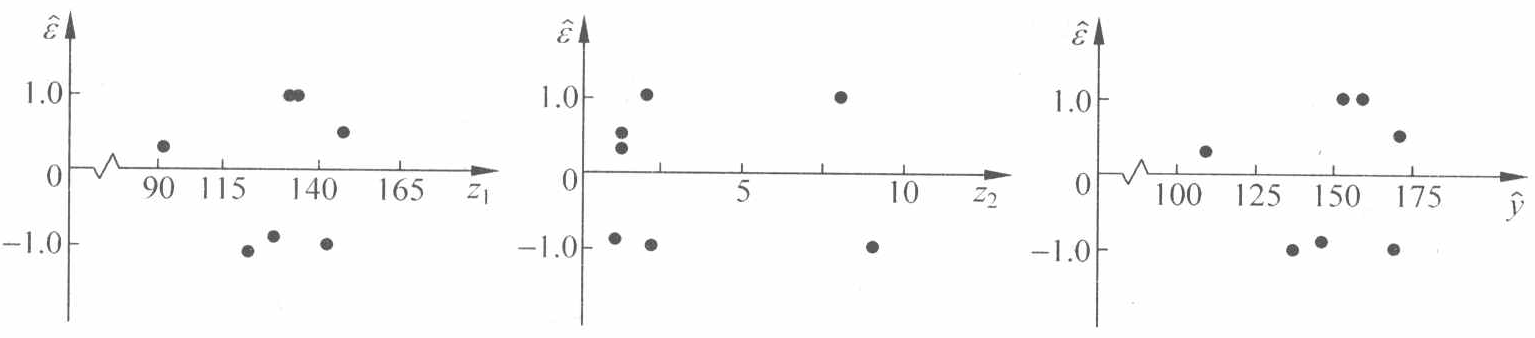
\includegraphics[width=130.0mm]{figs/fig_pg310_1.png}
\phantomsection\label{fig:7.3}\mvcap{图 7.3\quad 例 7.6 中计算机数据的残差图}
\end{mvfigure}

若对同一些预测变量值能得到若干个响应观测值, 则可以作一个拟合不足的形式检验.(见文献[13]中关于纯误差拟合不足检验的讨论.)

\subsection{杠杆率与影响}

虽然残差分析对评价模型的拟合情况很有用, 但是对回归模型的偏离往往隐藏在拟合过程之中. 例如, 响应变量或解释变量的数据中可能存在``离群值'', 它们对分析会产生很大影响, 但在考察残差图时却不易被发现. 事实上, 这些离群值可能对拟合结果起决定作用.

杠杆率 $h_{jj}$, 即 $\mathbf{H}=\mathbf{Z}(\mathbf{Z}'\mathbf{Z})^{-1}\mathbf{Z}$ 的 $(j,j)$ 对角元, 可以用两种方式解释. 首先, 在解释变量空间中, 杠杆率是第 $j$ 个数据点到其他 $n-1$ 个数据点距离远近的度量. 对于只有一个解释变量 $z$ 的简单线性回归,
\[
h_{jj}=\frac{1}{n}+\frac{(z_j-\bar{z})^2}{\sum\limits_{j=1}^{n}(z_j-\bar{z})^2}
\]
平均杠杆率是 $(r+1)/n$(见习题 7.8).

其次, 杠杆率是单个观测被从拟合中拖开程度的度量. 预测值向量
\[
\hat{\mathbf{y}}=\mathbf{Z}\hat{\boldsymbol{\beta}}=\mathbf{Z}(\mathbf{Z}'\mathbf{Z})^{-1}\mathbf{Z}\mathbf{y}=\mathbf{H}\mathbf{y}
\]
其中第 $j$ 行用观测值将拟合值 $\hat{y}_j$ 表示为
\[
\hat{y}_j=h_{jj}y_j+\sum_{k\neq j}h_{jk}y_k
\]
当所有其他 $y$ 值固定时,
\[
(\hat{y}_j\text{ 的变化})=h_{jj}(y_j\text{ 的变化})
\]
如果杠杆率相对于其他 $h_{jk}$ 比较大, 则 $y_j$ 对预测值 $\hat{y}_j$ 的贡献是主要的.

数据中对分析结果有显著影响的那些观测值称为\textbf{有影响的观测值}. 评估影响大小的方法是根据被考察的观测值被剔除后, 参数估计值向量 $\hat{\boldsymbol{\beta}}$ 的变化程度. 以杠杆率与影响分析统计量为基础的图, 以及它们在诊断性检查中的应用可在文献[3], [5]和[10]中找到.

如果在诊断性检查后没有发现对模型假定的严重背离, 我们就可以对 $\boldsymbol{\beta}$ 和未来的 $Y$ 值作推断, 并在某种程度上能保证不会被误导.

%% ===== pg-311 =====

% ---- pg-311 （书页 299） ----

\subsection{线性回归中的其他问题}

我们来简单讨论一下回归中的几个重要问题. 这些问题在回归分析的专著中得到了很大篇幅的讨论(见文献[10], [11], [13]和[23]).

\noindent\textbf{从一个大集合中选择预测变量}\quad 实践中往往很难立刻就得到一个合适的回归函数. 哪些预测变量应该被包含在模型中? 回归函数应取何种形式?

当可能的预测变量非常多时, 并非所有变量都应进入模型. 现在很容易找到选择``最佳''预测量子集的方法及有关计算机程序. 一类好办法是试用所有子集: 只用 $z_1$, 只用 $z_2$, 用 $z_1$ 和 $z_2$, $\cdots$, 等等. 最佳选择通过检查某个准则来确定, 常用的一个选择量是 $R^2$[见\hyperref[eq:7-9]{式(7-9)}]. 但是, $R^2$ 总是随着模型中变量的增加而增加. 虽然这个问题可以用修正的 $R^2$ 即 $\bar{R}^2=1-(1-R^2)(n-1)/(n-r-1)$ 来缓解, 但更好的变量选择准则可能应该是马罗(Mallow)的 $C_p$ 统计量(见文献[12]):
\[
C_p=\left(\frac{\left(\begin{array}{c}\text{包括常数项在内含 }p\text{ 个参数}\\[-0.3ex]\text{的子模型的残差平方和}\end{array}\right)}{(\text{全模型的残差方差})}\right)-(n-2p)
\]
对每个预测量子集作 $(p,C_p)$ 标绘图, 此图将显示出能很好预测响应观测值的模型. 典型的情况是: 好模型的 $(p,C_p)$ 坐标在 $45^\circ$ 线附近. 在\hyperref[fig:7.4]{图 7.4} 中, 我们用小圆圈来表示``最佳''预测变量子集.

\begin{mvfigure}
\begin{tikzpicture}[x=0.62cm,y=0.62cm,font=\small,line width=0.5pt]
% 坐标轴（带断轴）
\draw[->] (0,0)--(0,11.05);
\draw[->] (0,11.75)--(0,14.5);
% 断轴符号
\draw (-0.12,11.28)--(0.12,11.20)--(-0.12,11.45)--(0.12,11.37);
% 轴上的横虚线
\draw[dashed] (0.1,11.35)--(7.4,11.35);
% 45 度线
\draw (0,0)--(6,6);
% 横轴
\draw[->] (0,0)--(7.6,0) node[below right,inner sep=1pt] {$p=r+1$};
% 横轴刻度
\foreach \i in {1,...,7}{\draw (\i,0)--(\i,-0.18) node[below,inner sep=1pt] {\i};}
% 纵轴刻度（下半段）
\foreach \i in {1,...,11}{\draw (0,\i)--(-0.18,\i) node[left,inner sep=2pt] {\i};}
% 纵轴刻度（上半段）
\foreach \v/\lab in {11.75/{$1\,200$},12.8/{$1\,600$},13.85/{$1\,800$}}{\draw (0,\v)--(-0.18,\v) node[left,inner sep=2pt] {\lab};}
\node[left,inner sep=4pt] at (-0.6,7.0) {$C_p$};
% 数据点
\fill (1.15,13.85) circle (2.3pt); \node[right,inner sep=2pt] at (1.15,13.85) {$(0)$};
\fill (2.05,12.85) circle (2.3pt); \node[right,inner sep=2pt] at (2.05,12.85) {$(3)$};
\fill (1.45,12.35) circle (2.3pt); \node[right,inner sep=2pt] at (1.45,12.35) {$(2)$};
\fill (2.95,12.15) circle (2.3pt); \node[right,inner sep=2pt] at (2.95,12.15) {$(2,3)$};
\fill (2.90,10.55) circle (2.3pt); \node[right,inner sep=2pt] at (2.90,10.55) {$(1,3)$};
\fill (1.90,8.50) circle (2.3pt); \node[right,inner sep=2pt] at (1.90,8.50) {$(1)$};
\fill (3.05,2.60) circle (2.3pt); \draw (3.05,2.60) circle (4.6pt);
\node[right,inner sep=3pt] at (3.05,2.60) {$(1,2)$};
\fill (3.70,4.00) circle (2.3pt); \node[right,inner sep=2pt] at (3.70,4.00) {$(1,2,3)$};
\node[align=center] at (4.6,1.7) {括号中的数字代表\\预测变量的编号};
\end{tikzpicture}
\phantomsection\label{fig:7.4}\mvcap{图 7.4\quad 例 7.6 中计算机数据的 $\mathbf{C}_p$ 标绘图}
\mvcap{($z_1=$命令数, $z_2=$增删项目数, $z_3=$项目数)}
\end{mvfigure}

如果预测变量的数目非常多, 费用方面的考虑使能考察的模型个数受到限制. 另一种方法称为逐步回归法(见文献[13]), 这种方法力图选择重要的预测变量而不考虑所有可能性. 这种方法可用下列基本步骤来描述:

\noindent\textbf{步骤 1.}\quad 考虑所有可能的简单线性回归. 能够解释大部分 $Y$ 变差的预测变量(即与响应 $Y$ 相关最强的变量)是应首先被列入回归函数的变量.

\noindent\textbf{步骤 2.}\quad 下一个应被列入模型的变量是模型外变量中对回归平方和作出最显著贡献的那个变量. 贡献的显著性由 $F$ 检验确定(见结论 7.6). 在一个变量的贡献被认为显著之前必须超过的那个 $F$ 统计量的值, 常被称为 \textbf{$F$ 临界值}.

\noindent\textbf{步骤 3.}\quad 一旦又有某个变量进入了模型, 则应利用 $F$ 检验来检验回归方程中每一个原有变量对回归平方和贡献的显著性. 若 $F$ 统计量小于某个与指定显著性水平相对应的临界值, 就应将相应变量从回归函数中剔除.

\noindent\textbf{步骤 4.}\quad 将步骤 2 与步骤 3 不断重复, 直到所有可能增添的变量均不显著, 所有可能删除的变量均显著时为止.

由于整个过程是一步一步进行的, 不能保证这种方法能选出比如说三个``最佳''预测变

%% ===== pg-312 =====

% ---- pg-312 （书页 300） ----

量. 另一个缺点是: 这种(自动)选择方法不能显示在什么情况下变量的变换是有用的.

另一个选择适当模型的准则称为信息准则. 此准则也在残差平方和的大小和模型中参数个数之间寻求平衡.

赤池(Akaike)信息准则(AIC)是
\[
\text{AIC}=n\ln\left(\frac{\text{有 }p\text{ 个参数并含有截距的子模型的残差平方和}}{n}\right)+2p
\]
残差平方和应该小, 但是第二项惩罚过多的参数. 总体上, 我们希望选择具有较小 AIC 值的模型.

\noindent\textbf{共线性}\quad 若 $\mathbf{Z}$ 不满秩, 则某些线性组合, 例如 $\mathbf{Z}\mathbf{a}$, 必为 $\mathbf{0}$. 在这种情况下, 就说这些列是共线的. 这意味着 $\mathbf{Z}'\mathbf{Z}$ 没有逆阵. 就大多数回归分析而言, 不大可能恰好有 $\mathbf{Z}\mathbf{a}=\mathbf{0}$. 但如果 $\mathbf{Z}$ 矩阵诸列的线性组合接近于零, 则 $(\mathbf{Z}'\mathbf{Z})^{-1}$ 的计算值不稳定. 典型的情况是, $(\mathbf{Z}'\mathbf{Z})^{-1}$ 的对角元将很大. 这就使某些 $\hat{\beta}_j$ 的方差也很大, 这时很难发现``显著的''回归系数 $\beta_j$. 由共线性所引起的问题可通过下列方法得到一定程度的改善: (1) 将两个彼此强相关的预测变量之一剔除; 或 (2) 将响应 $Y$ 与预测变量的主成分联系起来. 也就是说, 将 $\mathbf{Z}$ 的各行 $\mathbf{z}_j'$ 看成一个样本, 按后面 8.3 节中将描述的方法计算前几个主成分, 然后用这些主成分作为新的``回归变量''对 $Y$ 作回归.

\noindent\textbf{由模型定型错误引起的偏倚}\quad 假定某些重要的预测变量未被选进模型, 也就是说, 假定真正的模型应该是 $\mathbf{Z}=[\mathbf{Z}_1\;\mathbf{Z}_2]$, 秩为 $r+1$, 且
\phantomsection\label{eq:7-20}
\begin{equation}
\underset{(n\times1)}{\mathbf{Y}}=\left[\begin{array}{c:c}\underset{(n\times(q+1))}{\mathbf{Z}_1}&\underset{(n\times(r-q))}{\mathbf{Z}_2}\end{array}\right]\left[\begin{array}{c}\underset{((q+1)\times1)}{\boldsymbol{\beta}_{(1)}}\\\hdashline\underset{((r-q)\times1)}{\boldsymbol{\beta}_{(2)}}\end{array}\right]+\underset{(n\times1)}{\boldsymbol{\epsilon}} \tag{7-20}
\end{equation}
\[
=\mathbf{Z}_1\boldsymbol{\beta}_{(1)}+\mathbf{Z}_2\boldsymbol{\beta}_{(2)}+\boldsymbol{\epsilon}
\]
其中 $E(\boldsymbol{\epsilon})=\mathbf{0}$, 且 $\operatorname{Var}(\boldsymbol{\epsilon})=\sigma^2\mathbf{I}$. 但是, 研究者在使误差平方和 $(\mathbf{Y}-\mathbf{Z}_1\boldsymbol{\beta}_{(1)})'(\mathbf{Y}-\mathbf{Z}_1\boldsymbol{\beta}_{(1)})$ 极小化时只用了前 $q$ 个变量. $\boldsymbol{\beta}_{(1)}$ 的最小二乘估计量为 $\hat{\boldsymbol{\beta}}_{(1)}=(\mathbf{Z}_1'\mathbf{Z}_1)^{-1}\mathbf{Z}_1'\mathbf{Y}$. 这时, 与模型正确定型时的情形不同,
\phantomsection\label{eq:7-21}
\begin{equation}
\begin{aligned}
E(\hat{\boldsymbol{\beta}}_{(1)})&=(\mathbf{Z}_1'\mathbf{Z}_1)^{-1}\mathbf{Z}_1'E(\mathbf{Y})=(\mathbf{Z}_1'\mathbf{Z}_1)^{-1}\mathbf{Z}_1'(\mathbf{Z}_1\boldsymbol{\beta}_{(1)}+\mathbf{Z}_2\boldsymbol{\beta}_{(2)}+E(\boldsymbol{\epsilon}))\\
&=\boldsymbol{\beta}_{(1)}+(\mathbf{Z}_1'\mathbf{Z}_1)^{-1}\mathbf{Z}_1'\mathbf{Z}_2\boldsymbol{\beta}_{(2)}
\end{aligned} \tag{7-21}
\end{equation}
也就是说, 除非 $\mathbf{Z}_1$ 的列与 $\mathbf{Z}_2$ 的列相互垂直(也就是说, $\mathbf{Z}_1'\mathbf{Z}_2=\mathbf{0}$), $\hat{\boldsymbol{\beta}}_{(1)}$ 为 $\boldsymbol{\beta}_{(1)}$ 的有偏估计量. 若重要的变量被遗弃在模型之外, 最小二乘估计量 $\hat{\boldsymbol{\beta}}_{(1)}$ 可能会把人引入歧途.

\section{多元多重回归}
\phantomsection\label{sec:7.7}

在本节中, 我们考虑 $m$ 个响应变量 $Y_1,Y_2,\cdots,Y_m$ 与同一个预测变量集 $z_1,z_2,\cdots,z_r$ 之间的关系. 假定每个响应有自己的回归模型:
\phantomsection\label{eq:7-22}
\begin{equation}
\begin{aligned}
Y_1&=\beta_{01}+\beta_{11}z_1+\cdots+\beta_{r1}z_r+\epsilon_1\\
Y_2&=\beta_{02}+\beta_{12}z_1+\cdots+\beta_{r2}z_r+\epsilon_2\\
&\qquad\vdots\qquad\qquad\vdots\\
Y_m&=\beta_{0m}+\beta_{1m}z_1+\cdots+\beta_{rm}z_r+\epsilon_m
\end{aligned} \tag{7-22}
\end{equation}
误差项 $\boldsymbol{\epsilon}'=[\epsilon_1,\epsilon_2,\cdots,\epsilon_m]$ 有 $E(\boldsymbol{\epsilon})=\mathbf{0}$ 和 $\operatorname{Var}(\boldsymbol{\epsilon})=\boldsymbol{\Sigma}$. 这样, 与不同响应相联系的误差项可以彼此相关.

%% ===== pg-313 =====

% ---- pg-313 （书页 301） ----

为建立与经典线性回归模型相一致的符号体系, 以 $[\mathbf{z}_{j0},z_{j1},\cdots,z_{jr}]$ 代表第 $j$ 次试验中的预测变量值, 以 $\mathbf{Y}_j=[Y_{j1},Y_{j2},\cdots,Y_{jm}]'$ 代表响应, 以 $\boldsymbol{\epsilon}_j=[\epsilon_{j1},\epsilon_{j2},\cdots,\epsilon_{jm}]'$ 代表误差. 用矩阵表示时, 设计阵
\[
\underset{(n\times(r+1))}{\mathbf{Z}}=\begin{bmatrix}z_{10}&z_{11}&\cdots&z_{1r}\\z_{20}&z_{21}&\cdots&z_{2r}\\\vdots&\vdots&&\vdots\\z_{n0}&z_{n1}&\cdots&z_{nr}\end{bmatrix}
\]
与单响应回归模型的情况相同[见\hyperref[eq:7-3]{式(7-3)}]. 其他矩阵量皆有多元对应量. 令
\[
\underset{(n\times m)}{\mathbf{Y}}=\begin{bmatrix}Y_{11}&Y_{12}&\cdots&Y_{1m}\\Y_{21}&Y_{22}&\cdots&Y_{2m}\\\vdots&\vdots&&\vdots\\Y_{n1}&Y_{n2}&\cdots&Y_{nm}\end{bmatrix}=\left[\mathbf{Y}_{(1)}\;\vdots\;\mathbf{Y}_{(2)}\;\vdots\;\cdots\;\vdots\;\mathbf{Y}_{(m)}\right]
\]
\[
\underset{((r+1)\times m)}{\boldsymbol{\beta}}=\begin{bmatrix}\beta_{01}&\beta_{02}&\cdots&\beta_{0m}\\\beta_{11}&\beta_{12}&\cdots&\beta_{1m}\\\vdots&\vdots&&\vdots\\\beta_{r1}&\beta_{r2}&\cdots&\beta_{rm}\end{bmatrix}=\left[\boldsymbol{\beta}_{(1)}\;\vdots\;\boldsymbol{\beta}_{(2)}\;\vdots\;\cdots\;\vdots\;\boldsymbol{\beta}_{(m)}\right]
\]
\[
\underset{(n\times m)}{\boldsymbol{\epsilon}}=\begin{bmatrix}\epsilon_{11}&\epsilon_{12}&\cdots&\epsilon_{1m}\\\epsilon_{21}&\epsilon_{22}&\cdots&\epsilon_{2m}\\\vdots&\vdots&&\vdots\\\epsilon_{n1}&\epsilon_{n2}&\cdots&\epsilon_{nm}\end{bmatrix}=\left[\boldsymbol{\epsilon}_{(1)}\;\vdots\;\boldsymbol{\epsilon}_{(2)}\;\vdots\;\cdots\;\vdots\;\boldsymbol{\epsilon}_{(m)}\right]
\]
\[
=\left[\begin{array}{c}\boldsymbol{\epsilon}_1'\\\hdashline\boldsymbol{\epsilon}_2'\\\hdashline\vdots\\\hdashline\boldsymbol{\epsilon}_n'\end{array}\right]
\]

\begin{mvbox}
{\centering\textbf{多元线性回归模型}\par}
\phantomsection\label{eq:7-23}
\begin{equation}
\underset{(n\times m)}{\mathbf{Y}}=\underset{(n\times(r+1))}{\mathbf{Z}}\quad\underset{((r+1)\times m)}{\boldsymbol{\beta}}+\underset{(n\times m)}{\boldsymbol{\epsilon}} \tag{7-23}
\end{equation}
其中 $E(\boldsymbol{\epsilon}_{(i)})=\mathbf{0}$, $\operatorname{Cov}(\boldsymbol{\epsilon}_{(i)},\boldsymbol{\epsilon}_{(k)})=\sigma_{ik}\mathbf{I}$ \quad $i,k=1,2,\cdots,m$.

第 $j$ 次试验的 $m$ 个观测值有协方差阵 $\boldsymbol{\Sigma}=\{\sigma_{ik}\}$, 但来自不同试验的观测值不相关. 这里 $\boldsymbol{\beta}$ 和 $\sigma_{ik}$ 是未知参数, 设计阵 $\mathbf{Z}$ 的第 $j$ 行为 $[\mathbf{z}_{j0},z_{j1},\cdots,z_{jr}]$.
\end{mvbox}

简单地说, 第 $i$ 个响应 $\mathbf{Y}_{(i)}$ 服从线性回归模型
\phantomsection\label{eq:7-24}
\begin{equation}
\mathbf{Y}_{(i)}=\mathbf{Z}\boldsymbol{\beta}_{(i)}+\boldsymbol{\epsilon}_{(i)},\qquad i=1,2,\cdots,m \tag{7-24}
\end{equation}
且 $\operatorname{Cov}(\boldsymbol{\epsilon}_{(i)})=\sigma_{ii}\mathbf{I}$. 但同一次试验中不同响应的误差可以相关.

给定预测变量的值 $\mathbf{Z}$ 和结果变量 $\mathbf{Y}$, 我们只用第 $i$ 个响应的观测值 $\mathbf{Y}_{(i)}$ 来确定 $\boldsymbol{\beta}_{(i)}$ 的最小二乘估计. 为保持与单响应解一致, 我们取
\phantomsection\label{eq:7-25}
\begin{equation}
\hat{\boldsymbol{\beta}}_{(i)}=(\mathbf{Z}'\mathbf{Z})^{-1}\mathbf{Z}'\mathbf{Y}_{(i)} \tag{7-25}
\end{equation}
将这些单变量最小二乘估计放在一起, 我们有
\[
\hat{\boldsymbol{\beta}}=\left[\hat{\boldsymbol{\beta}}_{(1)}\;\vdots\;\hat{\boldsymbol{\beta}}_{(2)}\;\vdots\;\cdots\;\vdots\;\hat{\boldsymbol{\beta}}_{(m)}\right]=(\mathbf{Z}'\mathbf{Z})^{-1}\mathbf{Z}'\left[\mathbf{Y}_{(1)}\;\vdots\;\mathbf{Y}_{(2)}\;\vdots\;\cdots\;\vdots\;\mathbf{Y}_{(m)}\right]
\]

%% ===== pg-314 =====

% ---- pg-314 （书页 302） ----

或
\phantomsection\label{eq:7-26}
\begin{equation}
\hat{\boldsymbol{\beta}}=(\mathbf{Z}'\mathbf{Z})^{-1}\mathbf{Z}'\mathbf{Y} \tag{7-26}
\end{equation}
对参数的任一选择 $\mathbf{B}=[\mathbf{b}_{(1)}\;\vdots\;\mathbf{b}_{(2)}\;\vdots\;\cdots\;\vdots\;\mathbf{b}_{(m)}]$, 误差矩阵为 $\mathbf{Y}-\mathbf{Z}\mathbf{B}$. 误差的平方与交叉乘积之和的矩阵为
\phantomsection\label{eq:7-27}
\begin{equation}
\begin{aligned}
&(\mathbf{Y}-\mathbf{Z}\mathbf{B})'(\mathbf{Y}-\mathbf{Z}\mathbf{B})\\
&\quad=\begin{bmatrix}(Y_{(1)}-\mathbf{Z}\mathbf{b}_{(1)})'(Y_{(1)}-\mathbf{Z}\mathbf{b}_{(1)})&\cdots&(Y_{(1)}-\mathbf{Z}\mathbf{b}_{(1)})'(Y_{(m)}-\mathbf{Z}\mathbf{b}_{(m)})\\\vdots&&\vdots\\(Y_{(m)}-\mathbf{Z}\mathbf{b}_{(m)})'(Y_{(1)}-\mathbf{Z}\mathbf{b}_{(1)})&\cdots&(Y_{(m)}-\mathbf{Z}\mathbf{b}_{(m)})'(Y_{(m)}-\mathbf{Z}\mathbf{b}_{(m)})\end{bmatrix}
\end{aligned} \tag{7-27}
\end{equation}
选择 $\mathbf{b}_{(i)}=\hat{\boldsymbol{\beta}}_{(i)}$ 能使第 $i$ 个对角平方和 $(Y_{(i)}-\mathbf{Z}\mathbf{b}_{(i)})'(Y_{(i)}-\mathbf{Z}\mathbf{b}_{(i)})$ 极小化. 因而, 当选择 $\mathbf{B}=\hat{\boldsymbol{\beta}}$ 时, $\operatorname{tr}[(\mathbf{Y}-\mathbf{Z}\mathbf{B})'(\mathbf{Y}-\mathbf{Z}\mathbf{B})]$ 达到最小. 同时, ``广义方差''$|(\mathbf{Y}-\mathbf{Z}\mathbf{B})'(\mathbf{Y}-\mathbf{Z}\mathbf{B})|$ 也在最小二乘估计 $\hat{\boldsymbol{\beta}}$ 处达到最小(其他广义平方和性质见练习 7.11).

用最小二乘估计 $\hat{\boldsymbol{\beta}}$, 我们可以构造以下两个矩阵:
\[
\text{预测值矩阵: }\hat{\mathbf{Y}}=\mathbf{Z}\hat{\boldsymbol{\beta}}=\mathbf{Z}(\mathbf{Z}'\mathbf{Z})^{-1}\mathbf{Z}'\mathbf{Y}
\]
\phantomsection\label{eq:7-28}
\begin{equation}
\text{残差矩阵: }\hat{\boldsymbol{\epsilon}}=\mathbf{Y}-\hat{\mathbf{Y}}=[\mathbf{I}-\mathbf{Z}(\mathbf{Z}'\mathbf{Z})^{-1}\mathbf{Z}']\mathbf{Y} \tag{7-28}
\end{equation}
在经典线性回归中残差、预测值和 $\mathbf{Z}$ 的各列之间的正交性在多元多重回归中也成立. 这是由于 $\mathbf{Z}'[\mathbf{I}-\mathbf{Z}(\mathbf{Z}'\mathbf{Z})^{-1}\mathbf{Z}']=\mathbf{Z}'-\mathbf{Z}'=\mathbf{0}$ 之故. 具体说,
\phantomsection\label{eq:7-29}
\begin{equation}
\mathbf{Z}'\hat{\boldsymbol{\epsilon}}=\mathbf{Z}'[\mathbf{I}-\mathbf{Z}(\mathbf{Z}'\mathbf{Z})^{-1}\mathbf{Z}']\mathbf{Y}=\mathbf{0} \tag{7-29}
\end{equation}
故残差 $\hat{\boldsymbol{\epsilon}}_{(i)}$ 垂直于 $\mathbf{Z}$ 的各列. 又因
\phantomsection\label{eq:7-30}
\begin{equation}
\hat{\mathbf{Y}}'\hat{\boldsymbol{\epsilon}}=\hat{\boldsymbol{\beta}}'\mathbf{Z}'[\mathbf{I}-\mathbf{Z}(\mathbf{Z}'\mathbf{Z})^{-1}\mathbf{Z}']\mathbf{Y}=\mathbf{0} \tag{7-30}
\end{equation}
由此确认第 $i$ 个响应的预测值垂直于残差 $\hat{\boldsymbol{\epsilon}}_{(i)}$. 由于 $\mathbf{Y}=\hat{\mathbf{Y}}+\hat{\boldsymbol{\epsilon}}$,
\[
\mathbf{Y}'\mathbf{Y}=(\hat{\mathbf{Y}}+\hat{\boldsymbol{\epsilon}})'(\hat{\mathbf{Y}}+\hat{\boldsymbol{\epsilon}})=\hat{\mathbf{Y}}'\hat{\mathbf{Y}}+\hat{\boldsymbol{\epsilon}}'\hat{\boldsymbol{\epsilon}}+\mathbf{0}+\mathbf{0}'
\]
或
\phantomsection\label{eq:7-31}
\begin{equation}
\underset{\substack{\text{(总的平方与}\\\text{交叉乘积之和)}}}{\mathbf{Y}'\mathbf{Y}}=\underset{\substack{\text{(预测的平方与}\\\text{交叉乘积之和)}}}{\hat{\mathbf{Y}}'\hat{\mathbf{Y}}}+\underset{\substack{\text{(误差的平方与}\\\text{交叉乘积之和)}}}{\hat{\boldsymbol{\epsilon}}'\hat{\boldsymbol{\epsilon}}} \tag{7-31}
\end{equation}
残差平方与交叉乘积之和也可写成
\phantomsection\label{eq:7-32}
\begin{equation}
\hat{\boldsymbol{\epsilon}}'\hat{\boldsymbol{\epsilon}}=\mathbf{Y}'\mathbf{Y}-\hat{\mathbf{Y}}'\hat{\mathbf{Y}}=\mathbf{Y}'\mathbf{Y}-\hat{\boldsymbol{\beta}}'\mathbf{Z}'\mathbf{Z}\hat{\boldsymbol{\beta}} \tag{7-32}
\end{equation}

\noindent\textbf{例 7.8}\quad (拟合多元直线回归模型)

为说明 $\hat{\boldsymbol{\beta}}$, $\hat{\mathbf{Y}}$ 和 $\hat{\boldsymbol{\epsilon}}$ 的计算, 我们拟合有两个响应 $Y_1$, $Y_2$ 及一个预测量 $z_1$ 的直线回归模型
\[
Y_{j1}=\beta_{01}+\beta_{11}z_{j1}+\epsilon_{j1}
\]
\[
Y_{j2}=\beta_{02}+\beta_{12}z_{j1}+\epsilon_{j2},\qquad j=1,2,\cdots,5
\]
所用数据为例 7.3 中的数据再加上一个响应变量的观测值:

\begin{mvtable}
\begin{tabular}{c|ccccc}
\hline
$z_1$ & 0 & 1 & 2 & 3 & 4\\
\hline
$y_1$ & 1 & 4 & 3 & 8 & 9\\
$y_2$ & $-1$ & $-1$ & 2 & 3 & 2\\
\hline
\end{tabular}
\end{mvtable}

%% ===== pg-315 =====

% ---- pg-315 （书页 303） ----

设计矩阵与在单响应变量问题中一样. 我们有
\[
\mathbf{Z}'=\begin{bmatrix}1&1&1&1&1\\0&1&2&3&4\end{bmatrix}\qquad(\mathbf{Z}'\mathbf{Z})^{-1}=\begin{bmatrix}0.6&-0.2\\-0.2&0.1\end{bmatrix}
\]
及
\[
\mathbf{Z}'\mathbf{y}_{(2)}=\begin{bmatrix}1&1&1&1&1\\0&1&2&3&4\end{bmatrix}\begin{bmatrix}-1\\-1\\2\\3\\2\end{bmatrix}=\begin{bmatrix}5\\20\end{bmatrix}
\]
故
\[
\hat{\boldsymbol{\beta}}_{(2)}=(\mathbf{Z}'\mathbf{Z})^{-1}\mathbf{Z}'\mathbf{y}_{(2)}=\begin{bmatrix}0.6&-0.2\\-0.2&0.1\end{bmatrix}\begin{bmatrix}5\\20\end{bmatrix}=\begin{bmatrix}-1\\1\end{bmatrix}
\]
由例 7.3,
\[
\hat{\boldsymbol{\beta}}_{(1)}=(\mathbf{Z}'\mathbf{Z})^{-1}\mathbf{Z}'\mathbf{y}_{(1)}=\begin{bmatrix}1\\2\end{bmatrix}
\]
因此,
\[
\hat{\boldsymbol{\beta}}=\left[\hat{\boldsymbol{\beta}}_{(1)}\;\vdots\;\hat{\boldsymbol{\beta}}_{(2)}\right]=\begin{bmatrix}1&-1\\2&1\end{bmatrix}=(\mathbf{Z}'\mathbf{Z})^{-1}\mathbf{Z}'\left[\mathbf{y}_{(1)}\;\vdots\;\mathbf{y}_{(2)}\right]
\]
于是预测方程为 $\hat{y}_1=1+2z_1$, 及 $\hat{y}_2=-1+z_2$. 用矩阵表示,
\[
\hat{\mathbf{Y}}=\mathbf{Z}\hat{\boldsymbol{\beta}}=\begin{bmatrix}1&0\\1&1\\1&2\\1&3\\1&4\end{bmatrix}\begin{bmatrix}1&-1\\2&1\end{bmatrix}=\begin{bmatrix}1&-1\\3&0\\5&1\\7&2\\9&3\end{bmatrix}
\]
\[
\hat{\boldsymbol{\epsilon}}=\mathbf{Y}-\hat{\mathbf{Y}}=\begin{bmatrix}0&1&-2&1&0\\0&-1&1&1&-1\end{bmatrix}'
\]
注意到
\[
\hat{\boldsymbol{\epsilon}}'\hat{\mathbf{Y}}=\begin{bmatrix}0&1&-2&1&0\\0&-1&1&1&-1\end{bmatrix}\begin{bmatrix}1&-1\\3&0\\5&1\\7&2\\9&3\end{bmatrix}=\begin{bmatrix}0&0\\0&0\end{bmatrix}
\]
由于
\[
\mathbf{Y}'\mathbf{Y}=\begin{bmatrix}1&4&3&8&9\\-1&-1&2&3&2\end{bmatrix}\begin{bmatrix}1&-1\\4&-1\\3&2\\8&3\\9&2\end{bmatrix}=\begin{bmatrix}171&43\\43&19\end{bmatrix}
\]

%% ===== pg-316 =====

% ---- pg-316 （书页 304） ----

\[
\hat{\mathbf{Y}}'\hat{\mathbf{Y}}=\begin{bmatrix}165&45\\45&15\end{bmatrix}\qquad\hat{\boldsymbol{\epsilon}}'\hat{\boldsymbol{\epsilon}}=\begin{bmatrix}6&-2\\-2&4\end{bmatrix}
\]
平方与交叉乘积之和的分解式
\[
\mathbf{Y}'\mathbf{Y}=\hat{\mathbf{Y}}'\hat{\mathbf{Y}}+\hat{\boldsymbol{\epsilon}}'\hat{\boldsymbol{\epsilon}}
\]
很容易验证. \hfill$\blacksquare$

\begin{mvfigure}
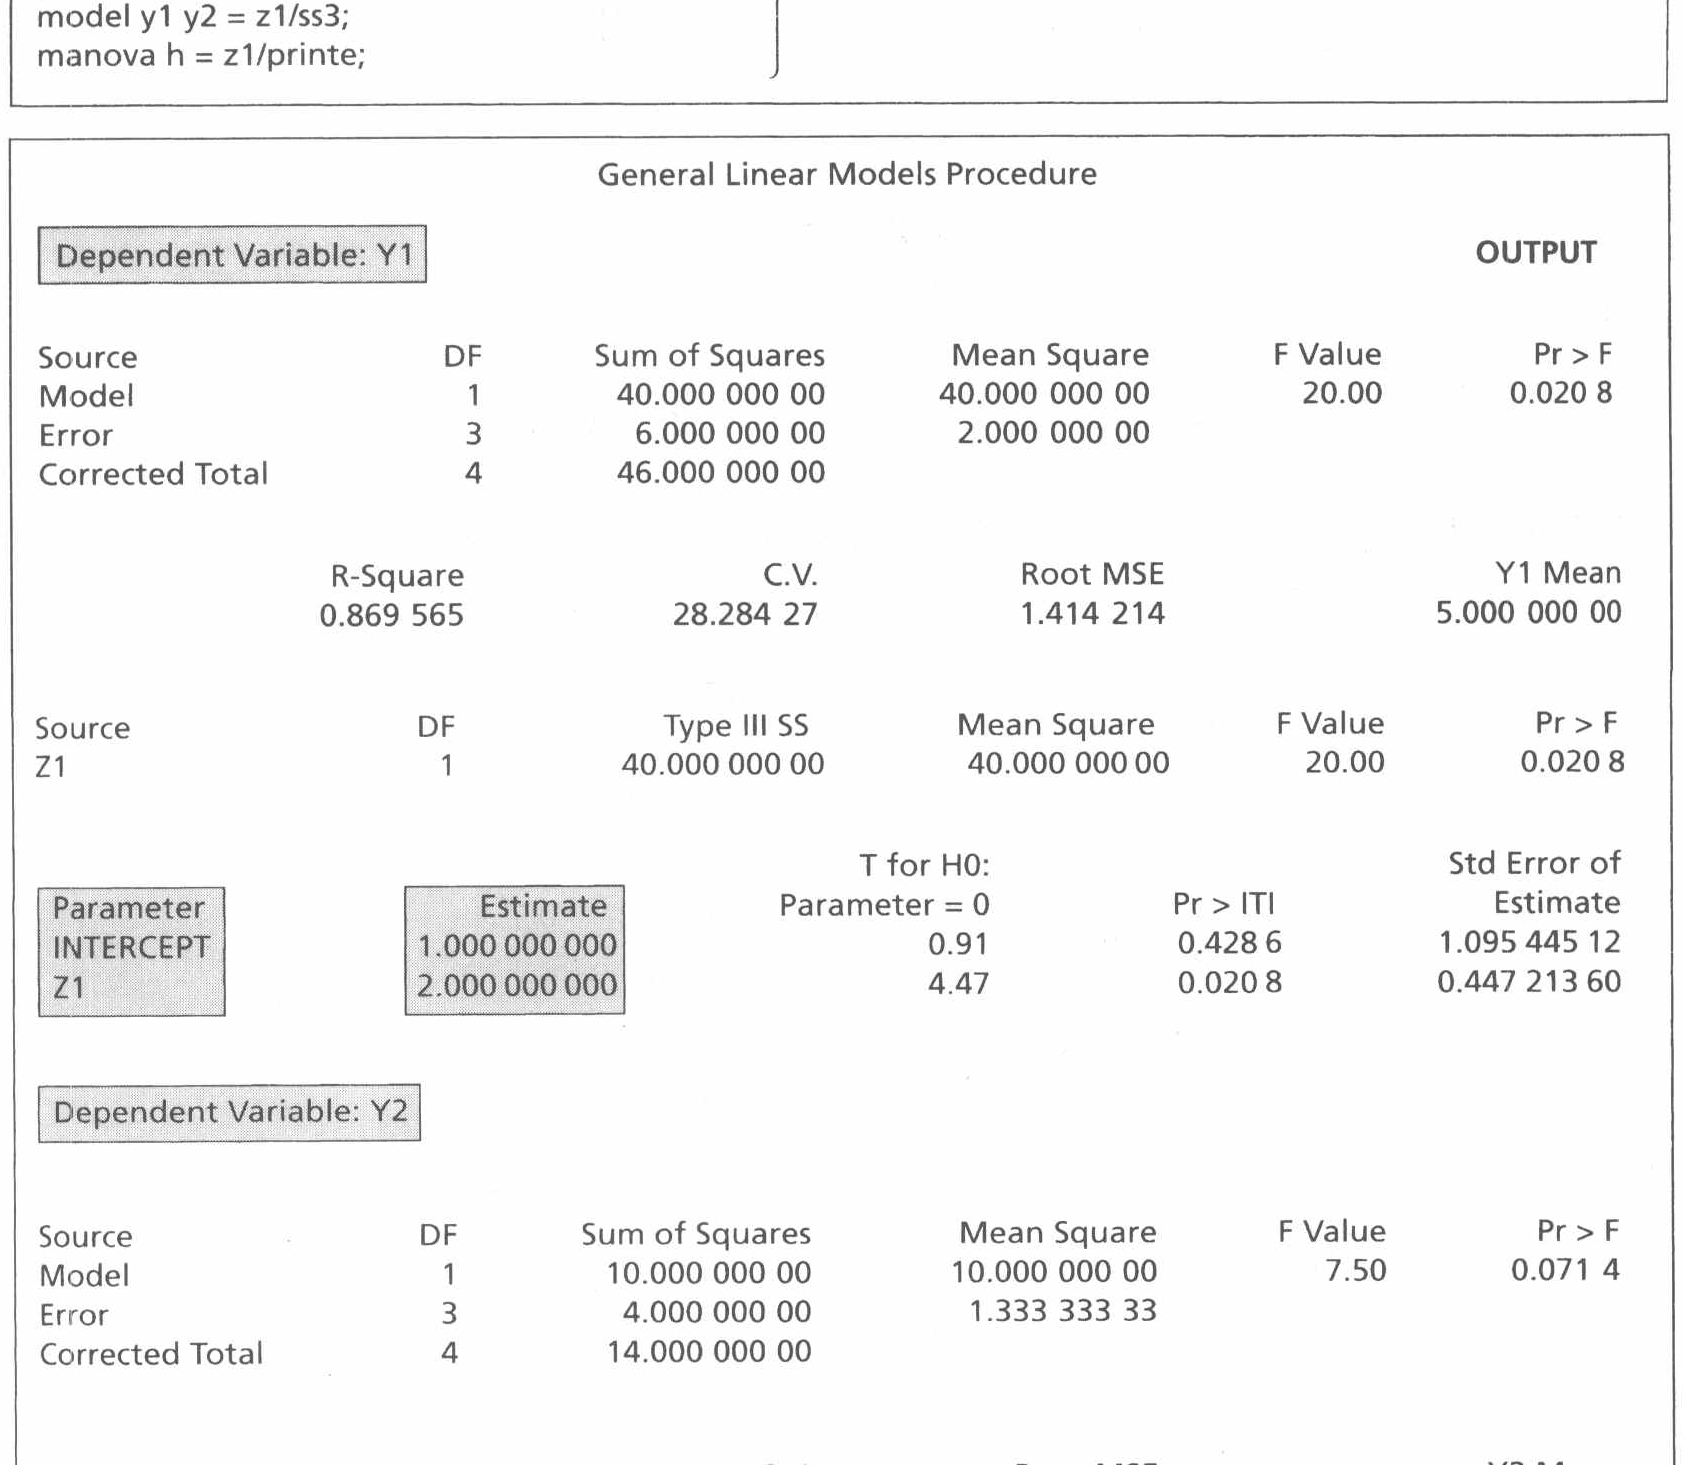
\includegraphics[width=141.0mm]{figs/fig_pg316_1.png}
\mvcap{显示板 7.2\quad 用 PROC. GLM 程序对例 7.8 中数据所做的 SAS 分析}
\end{mvfigure}

%% ===== pg-317 =====

% ---- pg-317 （书页 305） ----

\begin{mvframe}[显示板 7.2(续)]
\begin{center}
\begin{tabular}{lllll}
\toprule
Parameter & Estimate & T for H0: Parameter $=0$ & Pr $>|T|$ & Std Error of Estimate\\
\midrule
INTERCEPT & $-1.000\ 000\ 000$ & $-1.12$ & $0.345\ 0$ & $0.894\ 427\ 19$\\
Z1 & $1.000\ 000\ 000$ & $2.74$ & $0.071\ 4$ & $0.365\ 148\ 37$\\
\bottomrule
\end{tabular}

\medskip
\begin{tabular}{c}
E = Error SS \& CP Matrix
\end{tabular}

\medskip
\begin{tabular}{ccc}
 & Y1 & Y2\\
Y1 & 6 & $-2$\\
Y2 & $-2$ & 4\\
\end{tabular}

\medskip
\begin{tabular}{c}
Manova Test Criteria and Exact F Statistics for\\
the Hypothesis of no Overall Z1 Effect\\
H = Type III SS\&CP Matrix for Z1 \quad E = Error SS\&CP Matrix\\
S = 1 \quad M = 0 \quad N = 0
\end{tabular}

\medskip
\begin{tabular}{lrrrrr}
\toprule
Statistic & Value & F & Num DF & Den DF & Pr $>$ F\\
\midrule
Wilks' Lambda & 0.062 500 00 & 15.000 0 & 2 & 2 & 0.062 5\\
Pillai's Trace & 0.937 500 00 & 15.000 0 & 2 & 2 & 0.062 5\\
Hotelling-Lawley Trace & 15.000 000 00 & 15.000 0 & 2 & 2 & 0.062 5\\
Roy's Greatest Root & 15.000 000 00 & 15.000 0 & 2 & 2 & 0.062 5\\
\bottomrule
\end{tabular}
\end{center}
\end{mvframe}

\mvthm{结论 7.9}{对模型(7-23)及满秩 $(\mathbf{Z})=r+1<n$, 最小二乘估计量
$\hat{\boldsymbol{\beta}}=\left[\begin{array}{c:c:c:c}\hat{\boldsymbol{\beta}}_{(1)}&\hat{\boldsymbol{\beta}}_{(2)}&\cdots&\hat{\boldsymbol{\beta}}_{(m)}\end{array}\right]$
满足}
\[
E(\hat{\boldsymbol{\beta}}_{(i)})=\boldsymbol{\beta}_{(i)},\qquad E(\hat{\boldsymbol{\beta}})=\boldsymbol{\beta}
\]
且
\[
\operatorname{Cov}(\hat{\boldsymbol{\beta}}_{(i)},\hat{\boldsymbol{\beta}}_{(k)})=\sigma_{ik}(\mathbf{Z}'\mathbf{Z})^{-1},\qquad i,k=1,2,\cdots,m
\]
残差
$\hat{\boldsymbol{\epsilon}}=\left[\begin{array}{c:c:c:c}\hat{\boldsymbol{\epsilon}}_{(1)}&\hat{\boldsymbol{\epsilon}}_{(2)}&\cdots&\hat{\boldsymbol{\epsilon}}_{(m)}\end{array}\right]=\mathbf{Y}-\mathbf{Z}\hat{\boldsymbol{\beta}}$,
满足 $E(\hat{\boldsymbol{\epsilon}}_{(i)})=\mathbf{0}$ 且 $E(\hat{\boldsymbol{\epsilon}}_{(i)}'\hat{\boldsymbol{\epsilon}}_{(k)})=(n-r-1)\sigma_{ik}$, 故
\[
E(\hat{\boldsymbol{\epsilon}})=\mathbf{0}\qquad E\left(\frac{1}{n-r-1}\hat{\boldsymbol{\epsilon}}'\hat{\boldsymbol{\epsilon}}\right)=\boldsymbol{\Sigma}
\]
此外, $\hat{\boldsymbol{\epsilon}}$ 和 $\hat{\boldsymbol{\beta}}$ 不相关.

\medskip
\noindent\textbf{证明}\quad 第 $i$ 个响应服从多重回归模型
\[
\mathbf{Y}_{(i)}=\mathbf{Z}\boldsymbol{\beta}_{(i)}+\boldsymbol{\epsilon}_{(i)},\quad
E(\boldsymbol{\epsilon}_{(i)})=\mathbf{0},\quad
E(\boldsymbol{\epsilon}_{(i)}\boldsymbol{\epsilon}_{(i)}')=\sigma_{ii}\mathbf{I}
\]
又, 如同\hyperref[eq:7-24]{式(7-24)}中那样有
\phantomsection\label{eq:7-33}
\begin{equation}
\hat{\boldsymbol{\beta}}_{(i)}-\boldsymbol{\beta}_{(i)}
=(\mathbf{Z}'\mathbf{Z})^{-1}\mathbf{Z}'\mathbf{Y}_{(i)}-\boldsymbol{\beta}_{(i)}
=(\mathbf{Z}'\mathbf{Z})^{-1}\mathbf{Z}'\boldsymbol{\epsilon}_{(i)}
\tag{7-33}
\end{equation}
及
\[
\hat{\boldsymbol{\epsilon}}_{(i)}=\mathbf{Y}_{(i)}-\hat{\mathbf{Y}}_{(i)}
=[\mathbf{I}-\mathbf{Z}(\mathbf{Z}'\mathbf{Z})^{-1}\mathbf{Z}']\mathbf{Y}_{(i)}
=[\mathbf{I}-\mathbf{Z}(\mathbf{Z}'\mathbf{Z})^{-1}\mathbf{Z}']\boldsymbol{\epsilon}_{(i)}
\]
故 $E(\hat{\boldsymbol{\beta}}_{(i)})=\boldsymbol{\beta}_{(i)}$ 且 $E(\hat{\boldsymbol{\epsilon}}_{(i)})=\mathbf{0}$. 接下来, 有
\[
\begin{aligned}
\operatorname{Cov}(\hat{\boldsymbol{\beta}}_{(i)},\hat{\boldsymbol{\beta}}_{(k)})
&=E(\hat{\boldsymbol{\beta}}_{(i)}-\boldsymbol{\beta}_{(i)})(\hat{\boldsymbol{\beta}}_{(k)}-\boldsymbol{\beta}_{(k)})'\\
&=(\mathbf{Z}'\mathbf{Z})^{-1}\mathbf{Z}'E(\boldsymbol{\epsilon}_{(i)}\boldsymbol{\epsilon}_{(k)}')\mathbf{Z}(\mathbf{Z}'\mathbf{Z})^{-1}
=\sigma_{ik}(\mathbf{Z}'\mathbf{Z})^{-1}
\end{aligned}
\]
用结论 4.9 及结论 7.2 的证明, 对任意随机向量 $\mathbf{U}$ 和常数阵 $\mathbf{A}$, 我们有
$E[\mathbf{U}'\mathbf{A}\mathbf{U}]=$

%% ===== pg-318 =====

% ---- pg-318 （书页 306） ----

$E[\mathbf{U}'\mathbf{A}\mathbf{U}]=E[\operatorname{tr}(\mathbf{A}\mathbf{U}\mathbf{U}')]=\operatorname{tr}[\mathbf{A}E(\mathbf{U}\mathbf{U}')]$. 因此, 根据结论 7.1 的证明并利用结论 2A.12
\[
\begin{aligned}
E(\hat{\boldsymbol{\epsilon}}_{(i)}'\hat{\boldsymbol{\epsilon}}_{(k)})
&=E\left(\boldsymbol{\epsilon}_{(i)}'(\mathbf{I}-\mathbf{Z}(\mathbf{Z}'\mathbf{Z})^{-1}\mathbf{Z}')\boldsymbol{\epsilon}_{(k)}\right)
=\operatorname{tr}\left[(\mathbf{I}-\mathbf{Z}(\mathbf{Z}'\mathbf{Z})^{-1}\mathbf{Z}')\sigma_{ik}\mathbf{I}\right]\\
&=\sigma_{ik}\operatorname{tr}\left[(\mathbf{I}-\mathbf{Z}(\mathbf{Z}'\mathbf{Z})^{-1}\mathbf{Z}')\right]=\sigma_{ik}(n-r-1)
\end{aligned}
\]
对 $\hat{\boldsymbol{\epsilon}}'\hat{\boldsymbol{\epsilon}}$ 的每个元素 $\hat{\boldsymbol{\epsilon}}_{(i)}'\hat{\boldsymbol{\epsilon}}_{(k)}$ 除以 $n-r-1$, 我们得到 $\boldsymbol{\Sigma}$ 的无偏估计量. 最后,
\[
\begin{aligned}
\operatorname{Cov}(\hat{\boldsymbol{\beta}}_{(i)},\hat{\boldsymbol{\epsilon}}_{(k)})
&=E\left[(\mathbf{Z}'\mathbf{Z})^{-1}\mathbf{Z}'\boldsymbol{\epsilon}_{(i)}\boldsymbol{\epsilon}_{(k)}'(\mathbf{I}-\mathbf{Z}(\mathbf{Z}'\mathbf{Z})^{-1}\mathbf{Z}')\right]\\
&=(\mathbf{Z}'\mathbf{Z})^{-1}\mathbf{Z}'E(\boldsymbol{\epsilon}_{(i)}\boldsymbol{\epsilon}_{(k)}')(\mathbf{I}-\mathbf{Z}(\mathbf{Z}'\mathbf{Z})^{-1}\mathbf{Z}')\\
&=(\mathbf{Z}'\mathbf{Z})^{-1}\mathbf{Z}'\sigma_{ik}\mathbf{I}(\mathbf{I}-\mathbf{Z}(\mathbf{Z}'\mathbf{Z})^{-1}\mathbf{Z}')\\
&=\sigma_{ik}\left((\mathbf{Z}'\mathbf{Z})^{-1}\mathbf{Z}'-(\mathbf{Z}'\mathbf{Z})^{-1}\mathbf{Z}'\right)=\mathbf{0}
\end{aligned}
\]
故 $\hat{\boldsymbol{\beta}}$ 中的每个元素与 $\hat{\boldsymbol{\epsilon}}$ 中的每个元素不相关. \hfill$\blacksquare$

结论 7.9 中确定的均值向量和协方差阵能使我们得出最小二乘预测量的抽样性质.

我们首先考虑当预测变量取值 $\mathbf{z}_0=[1,z_{01},\cdots,z_{0r}]'$ 时均值向量的估计问题. 第 $i$ 个响应变量的均值是 $\mathbf{z}_0'\boldsymbol{\beta}_{(i)}$, 可用 $\mathbf{z}_0'\hat{\boldsymbol{\beta}}_{(i)}$(拟合回归关系的第 $i$ 个分量)来估计. 因此
\phantomsection\label{eq:7-34}
\begin{equation}
\mvfit{$\displaystyle
\mathbf{z}_0'\hat{\boldsymbol{\beta}}
=\left[\begin{array}{c:c:c:c}
\mathbf{z}_0'\hat{\boldsymbol{\beta}}_{(1)}&\mathbf{z}_0'\hat{\boldsymbol{\beta}}_{(2)}&\cdots&\mathbf{z}_0'\hat{\boldsymbol{\beta}}_{(m)}
\end{array}\right]
$} \tag{7-34}
\end{equation}
为 $\mathbf{z}_0'\boldsymbol{\beta}$ 的无偏估计量, 因为对每个分量均有 $E(\mathbf{z}_0'\hat{\boldsymbol{\beta}}_{(i)})=\mathbf{z}_0'E(\hat{\boldsymbol{\beta}}_{(i)})=\mathbf{z}_0'\boldsymbol{\beta}_{(i)}$. 由 $\hat{\boldsymbol{\beta}}_{(i)}$ 和 $\hat{\boldsymbol{\beta}}_{(k)}$ 的协方差阵得到估计误差 $\mathbf{z}_0'\boldsymbol{\beta}_{(i)}-\mathbf{z}_0'\hat{\boldsymbol{\beta}}_{(i)}$ 的协方差为
\phantomsection\label{eq:7-35}
\begin{equation}
\mvfit{$\displaystyle
\begin{aligned}
E\left[\mathbf{z}_0'(\boldsymbol{\beta}_{(i)}-\hat{\boldsymbol{\beta}}_{(i)})(\boldsymbol{\beta}_{(k)}-\hat{\boldsymbol{\beta}}_{(k)})'\mathbf{z}_0\right]
&=\mathbf{z}_0'\left(E(\boldsymbol{\beta}_{(i)}-\hat{\boldsymbol{\beta}}_{(i)})(\boldsymbol{\beta}_{(k)}-\hat{\boldsymbol{\beta}}_{(k)})'\right)\mathbf{z}_0\\
&=\sigma_{ik}\mathbf{z}_0'(\mathbf{Z}'\mathbf{Z})^{-1}\mathbf{z}_0
\end{aligned}
$} \tag{7-35}
\end{equation}
与此有关的问题是在 $\mathbf{z}_0$ 点预测新的观测值向量 $\mathbf{Y}_0=[Y_{01},Y_{02},\cdots,Y_{0m}]'$. 根据回归模型, $Y_{0i}=\mathbf{z}_0'\boldsymbol{\beta}_{(i)}+\epsilon_{0i}$, 其中“新”误差 $\boldsymbol{\epsilon}_0=[\epsilon_{01},\epsilon_{02},\cdots,\epsilon_{0m}]'$ 独立于误差 $\boldsymbol{\epsilon}$, 并满足 $E(\epsilon_{0i})=0$, 且 $E(\epsilon_{0i}\epsilon_{0k})=\sigma_{ik}$, 对 $\mathbf{Y}_0$ 的第 $i$ 个分量的预测误差为
\[
\begin{aligned}
Y_{0i}-\mathbf{z}_0'\hat{\boldsymbol{\beta}}_{(i)}
&=Y_{0i}-\mathbf{z}_0'\boldsymbol{\beta}_{(i)}+\mathbf{z}_0'\boldsymbol{\beta}_{(i)}-\mathbf{z}_0'\hat{\boldsymbol{\beta}}_{(i)}\\
&=\epsilon_{0i}-\mathbf{z}_0'(\hat{\boldsymbol{\beta}}_{(i)}-\boldsymbol{\beta}_{(i)})
\end{aligned}
\]
故 $E(Y_{0i}-\mathbf{z}_0'\hat{\boldsymbol{\beta}}_{(i)})=E(\epsilon_{0i})-\mathbf{z}_0'E(\hat{\boldsymbol{\beta}}_{(i)}-\boldsymbol{\beta}_{(i)})=0$, 说明 $\mathbf{z}_0'\hat{\boldsymbol{\beta}}_{(i)}$ 为 $Y_{0i}$ 的无偏预测量. 预测误差具有协方差
\phantomsection\label{eq:7-36}
\begin{equation}
\mvfit{$\displaystyle
\begin{aligned}
E(Y_{0i}-\mathbf{z}_0'\hat{\boldsymbol{\beta}}_{(i)})(Y_{0k}-\mathbf{z}_0'\hat{\boldsymbol{\beta}}_{(k)})
&=E\left(\epsilon_{0i}-\mathbf{z}_0'(\hat{\boldsymbol{\beta}}_{(i)}-\boldsymbol{\beta}_{(i)})\right)\left(\epsilon_{0k}-\mathbf{z}_0'(\hat{\boldsymbol{\beta}}_{(k)}-\boldsymbol{\beta}_{(k)})\right)\\
&=E(\epsilon_{0i}\epsilon_{0k})+\mathbf{z}_0'E(\hat{\boldsymbol{\beta}}_{(i)}-\boldsymbol{\beta}_{(i)})(\hat{\boldsymbol{\beta}}_{(k)}-\boldsymbol{\beta}_{(k)})'\mathbf{z}_0\\
&\quad-\mathbf{z}_0'E\left((\hat{\boldsymbol{\beta}}_{(i)}-\boldsymbol{\beta}_{(i)})\epsilon_{0k}\right)-E\left(\epsilon_{0i}(\hat{\boldsymbol{\beta}}_{(k)}-\boldsymbol{\beta}_{(k)})'\right)\mathbf{z}_0\\
&=\sigma_{ik}\left(1+\mathbf{z}_0'(\mathbf{Z}'\mathbf{Z})^{-1}\mathbf{z}_0\right)
\end{aligned}
$} \tag{7-36}
\end{equation}
注意 $E\left((\hat{\boldsymbol{\beta}}_{(i)}-\boldsymbol{\beta}_{(i)})\epsilon_{0k}\right)=\mathbf{0}$, 因为 $\hat{\boldsymbol{\beta}}_{(i)}=(\mathbf{Z}'\mathbf{Z})^{-1}\mathbf{Z}'\boldsymbol{\epsilon}_{(i)}+\boldsymbol{\beta}_{(i)}$ 与 $\boldsymbol{\epsilon}_0$ 独立. 类似的结论对 $E\left(\epsilon_{0i}(\hat{\boldsymbol{\beta}}_{(k)}-\boldsymbol{\beta}_{(k)})'\right)$ 也成立.

当误差 $\boldsymbol{\epsilon}$ 服从正态分布时, 可得出极大似然估计量及其分布.

\mvthm{结论 7.10}{} 设\hyperref[eq:7-23]{式(7-23)}中的多元多重回归模型成立, 有满秩 $(\mathbf{Z})=r+1$, $n\geqslant(r+1)+m$,

%% ===== pg-319 =====

% ---- pg-319 （书页 307） ----

且误差 $\boldsymbol{\epsilon}$ 服从正态分布. 此时
\[
\hat{\boldsymbol{\beta}}=(\mathbf{Z}'\mathbf{Z})^{-1}\mathbf{Z}'\mathbf{Y}
\]
为 $\boldsymbol{\beta}$ 的极大似然估计量, 且 $\hat{\boldsymbol{\beta}}$ 服从正态分布, 均值 $E(\hat{\boldsymbol{\beta}})=\boldsymbol{\beta}$, 且 $\operatorname{Cov}(\hat{\boldsymbol{\beta}}_{(i)},\hat{\boldsymbol{\beta}}_{(k)})=\sigma_{ik}(\mathbf{Z}'\mathbf{Z})^{-1}$. 此外, $\hat{\boldsymbol{\beta}}$ 独立于正定矩阵 $\boldsymbol{\Sigma}$ 的极大似然估计量
\[
\hat{\boldsymbol{\Sigma}}=\frac{1}{n}\hat{\boldsymbol{\epsilon}}'\hat{\boldsymbol{\epsilon}}
=\frac{1}{n}(\mathbf{Y}-\mathbf{Z}\hat{\boldsymbol{\beta}})'(\mathbf{Y}-\mathbf{Z}\hat{\boldsymbol{\beta}})
\]
且 $n\hat{\boldsymbol{\Sigma}}$ 服从分布 $W_{p,n-r-1}(\boldsymbol{\Sigma})$.

\medskip
\noindent\textbf{证明}\quad (见网页：www.prenhall.com/statistics) \hfill$\blacksquare$

结论 7.10 为最小二乘估计的采用提供了进一步支持. 当误差服从正态分布时, $\hat{\boldsymbol{\beta}}$ 与 $n^{-1}\hat{\boldsymbol{\epsilon}}'\hat{\boldsymbol{\epsilon}}$ 分别是 $\boldsymbol{\beta}$ 和 $\boldsymbol{\Sigma}$ 的极大似然估计量. 因此, 对大样本情形, 它们具有最小的可能方差.

\mvbold{评注}\quad 多元多重回归模型并没有提出新的计算问题. 最小二乘(极大似然)估计 $\hat{\boldsymbol{\beta}}_{(i)}=(\mathbf{Z}'\mathbf{Z})^{-1}\mathbf{Z}'\mathbf{y}_{(i)}$ 是对每个响应变量逐个计算的. 然而请注意: 模型要求对所有响应变量使用同一组预测变量.

一旦用数据拟合了一个多元多重回归模型, 就应该用 7.6 节中所介绍的诊断方法对这个模型做检查. 根据 4.6 节中介绍的方法, 考察残差向量 $[\hat{\epsilon}_{j1},\hat{\epsilon}_{j2},\cdots,\hat{\epsilon}_{jm}]$ 便可检查正态性是否满足或离群值是否存在.

本节剩余部分用来对正态理论下多元多重回归模型的推断作一简要讨论. 这些问题的展开讨论见文献[2]和[18].

\section{回归参数的似然比检验}
\phantomsection\label{sec:7.8}

单响应回归模型中的假设(7-12)的内容是: 响应变量不依赖于 $z_{q+1},z_{q+2},\cdots,z_r$. 设在多响应情况下该假设变为
\phantomsection\label{eq:7-37}
\begin{equation}
H_0: \boldsymbol{\beta}_{(2)}=\mathbf{0}\qquad \text{其中}\qquad
\boldsymbol{\beta}=\left[\begin{array}{c}
\underset{((q+1)\times m)}{\boldsymbol{\beta}_{(1)}}\\
\hdashline
\underset{((r-q)\times m)}{\boldsymbol{\beta}_{(2)}}
\end{array}\right]
\tag{7-37}
\end{equation}
令 $\mathbf{Z}=\left[\begin{array}{c:c}\underset{(n\times(q+1))}{\mathbf{Z}_1}&\underset{(n\times(r-q))}{\mathbf{Z}_2}\end{array}\right]$, 我们可将一般模型写成
\[
E(\mathbf{Y})=\mathbf{Z}\boldsymbol{\beta}
=\left[\begin{array}{c:c}\mathbf{Z}_1&\mathbf{Z}_2\end{array}\right]
\left[\begin{array}{c}\boldsymbol{\beta}_{(1)}\\ \hdashline \boldsymbol{\beta}_{(2)}\end{array}\right]
=\mathbf{Z}_1\boldsymbol{\beta}_{(1)}+\mathbf{Z}_2\boldsymbol{\beta}_{(2)}
\]
在假设 $H_0: \boldsymbol{\beta}_{(2)}=\mathbf{0}$ 下, $\mathbf{Y}=\mathbf{Z}_1\boldsymbol{\beta}_{(1)}+\boldsymbol{\epsilon}$, $H_0$ 的似然比检验建立在额外的平方与交叉乘积之和的基础之上:
\[
\begin{aligned}
&(\mathbf{Y}-\mathbf{Z}_1\hat{\boldsymbol{\beta}}_{(1)})'(\mathbf{Y}-\mathbf{Z}_1\hat{\boldsymbol{\beta}}_{(1)})-(\mathbf{Y}-\mathbf{Z}\hat{\boldsymbol{\beta}})'(\mathbf{Y}-\mathbf{Z}\hat{\boldsymbol{\beta}})\\
&=n(\hat{\boldsymbol{\Sigma}}_1-\hat{\boldsymbol{\Sigma}})
\end{aligned}
\]
其中 $\hat{\boldsymbol{\beta}}_{(1)}=(\mathbf{Z}_1'\mathbf{Z}_1)^{-1}\mathbf{Z}_1'\mathbf{Y}$, $\hat{\boldsymbol{\Sigma}}_1=n^{-1}(\mathbf{Y}-\mathbf{Z}_1\hat{\boldsymbol{\beta}}_{(1)})'(\mathbf{Y}-\mathbf{Z}_1\hat{\boldsymbol{\beta}}_{(1)})$. 根据结论 7.10, 可将似然比 $\Lambda$ 表为广义方差之比:
\phantomsection\label{eq:7-38}
\begin{equation}
\Lambda=\frac{\max\limits_{\boldsymbol{\beta}_{(1)},\boldsymbol{\Sigma}}L(\boldsymbol{\beta}_{(1)},\boldsymbol{\Sigma})}{\max\limits_{\boldsymbol{\beta},\boldsymbol{\Sigma}}L(\boldsymbol{\beta},\boldsymbol{\Sigma})}
=\frac{L(\hat{\boldsymbol{\beta}}_{(1)},\hat{\boldsymbol{\Sigma}}_1)}{L(\hat{\boldsymbol{\beta}},\hat{\boldsymbol{\Sigma}})}
=\left(\frac{|\hat{\boldsymbol{\Sigma}}|}{|\hat{\boldsymbol{\Sigma}}_1|}\right)^{n/2}
\tag{7-38}
\end{equation}

%% ===== pg-320 =====

% ---- pg-320 （书页 308） ----

因此可等价地采用威尔克斯 $\Lambda$ 统计量
\[
\Lambda^{2/n}=\frac{|\hat{\boldsymbol{\Sigma}}|}{|\hat{\boldsymbol{\Sigma}}_1|}
\]
\mvthm{结论 7.11}{设\hyperref[eq:7-23]{式(7-23)}中的多元多重回归模型成立, 有满秩$(\mathbf{Z})=r+1$, 且 $(r+1)+m\leqslant n$. 设误差 $\boldsymbol{\epsilon}$ 服从正态分布. 在假设 $H_0:\boldsymbol{\beta}_{(2)}=\mathbf{0}$ 下, $n\hat{\boldsymbol{\Sigma}}$ 服从 $W_{p,n-r-1}(\boldsymbol{\Sigma})$ 分布, 与 $n(\hat{\boldsymbol{\Sigma}}_1-\hat{\boldsymbol{\Sigma}})$ 独立, 而后者则服从 $W_{p,r-q}(\boldsymbol{\Sigma})$ 分布. $H_0$ 的似然比检验等价于当}
\[
-2\ln\Lambda=-n\ln\left(\frac{|\hat{\boldsymbol{\Sigma}}|}{|\hat{\boldsymbol{\Sigma}}_1|}\right)
=-n\ln\frac{|n\hat{\boldsymbol{\Sigma}}|}{|n\hat{\boldsymbol{\Sigma}}+n(\hat{\boldsymbol{\Sigma}}_1-\hat{\boldsymbol{\Sigma}})|}
\]
的值很大时拒绝 $H_0$. 对大的 $n$\footnote{{\footnotesize 从技术上说, $n-r$ 和 $n-m$ 也都应足够大, 才能得到好的 $\chi^2$ 近似.}}, 修正的统计量
\[
-\left[n-r-1-\frac{1}{2}(m-r+q+1)\right]\ln\left(\frac{|\hat{\boldsymbol{\Sigma}}|}{|\hat{\boldsymbol{\Sigma}}_1|}\right)
\]
作为相当好的近似, 服从自由度为 $(r-q)$ 的 $\chi^2$ 分布.

\medskip
\noindent\textbf{证明}\quad (见补充 7A.) \hfill$\blacksquare$

若 $\mathbf{Z}$ 并非满秩, 而是秩为 $r_1+1$, 则 $\hat{\boldsymbol{\beta}}=(\mathbf{Z}'\mathbf{Z})^-\mathbf{Z}'\mathbf{Y}$, 此处 $(\mathbf{Z}'\mathbf{Z})^-$ 为 $(\mathbf{Z}'\mathbf{Z})$ 的广义逆, 这在文献[22]中有详细讨论(又见练习 7.6). 结论 7.11 中有关分布的结论仍然正确, 但要用 $r_1$ 代替 $r$, 及用秩$(\mathbf{Z}_1)$代替 $q+1$. 然而在这种情况下并非所有关于 $\boldsymbol{\beta}$ 的假设都是可以检验的. 这是因为由 $\mathbf{Z}$ 的各列之间的相依性所造成的 $\boldsymbol{\beta}$ 的识别不具备唯一性. 尽管如此, 广义逆使得所有重要的 MANOVA 模型都可以作为多元多重回归模型的特殊情况来分析.

\medskip
\noindent\textbf{例 7.9}\quad (在多元响应下检验附加预测变量的重要性)

一个大型连锁饭店处于不同地点的三个分店的服务由一批男性和女性主顾根据两个质量指标进行了评估. 第一个服务质量指标已在例 7.5 中给出. 假定一个回归模型考虑了位置、性别和位置—性别交互作用三者对两个服务质量指标产生的效应. 设计矩阵(见例 7.5)对两个响应均保持不变. 我们用结论 7.11 来说明对“无位置—性别交互作用”这一假设的检验. 计算机程序给出
\[
\left(\begin{array}{c}\text{残差的平方与}\\\text{交叉乘积之和}\end{array}\right)
=n\hat{\boldsymbol{\Sigma}}
=\begin{bmatrix}2\ 977.39&1\ 021.72\\1\ 021.72&2\ 050.95\end{bmatrix}
\]
\[
\left(\begin{array}{c}\text{额外的平方与}\\\text{交叉乘积之和}\end{array}\right)
=n(\hat{\boldsymbol{\Sigma}}_1-\hat{\boldsymbol{\Sigma}})
=\begin{bmatrix}441.76&246.16\\246.16&366.12\end{bmatrix}
\]
令 $\boldsymbol{\beta}_{(2)}$ 为两个响应的交互作用参数矩阵. 虽然样本容量 $n=18$ 不大, 我们来说明结论 7.11 所提供的检验假设 $H_0:\boldsymbol{\beta}_{(2)}=\mathbf{0}$ 时所涉及的计算. 令 $\alpha=0.05$, 我们将
\[
\begin{aligned}
&-\left[n-r_1-1-\frac{1}{2}(m-r_1+q_1+1)\right]\ln\left(\frac{|n\hat{\boldsymbol{\Sigma}}|}{|n\hat{\boldsymbol{\Sigma}}+n(\hat{\boldsymbol{\Sigma}}_1-\hat{\boldsymbol{\Sigma}})|}\right)\\
&=-\left[18-5-1-\frac{1}{2}\times(2-5+3+1)\right]\times\ln(0.760\ 5)=3.28
\end{aligned}
\]
与自由度为 $m(r_1-q_1)=2\times2=4$ 的卡方百分点作比较, 以检验 $H_0$. 由于 $3.28<\chi_4^2(0.05)=$

%% ===== pg-321 =====

% ---- pg-321 （书页 309） ----

9.49, 我们在 5\% 的水平下不拒绝 $H_0$. 也就是说, 不需要交互作用项. \hfill$\blacksquare$

信息准则也能帮助选择简单但适当的多元多重回归模型. 对于连截距在内有 $d$ 个预测变量的模型, 令
\[
\hat{\boldsymbol{\Sigma}}_d=\frac{1}{n}(\text{残差平方及交叉乘积和矩阵})
\]
则赤池信息准则的多元多重回归版为
\[
\text{AIC}=n\ln(|\hat{\boldsymbol{\Sigma}}_d|)-2p\times d
\]
该准则在广义方差与参数数目之间寻求平衡. 具有较小 AIC 的模型优先考虑.

在例 7.9 中, 在无交互效应的零假设下, 我们有 $n=18$, $p=2$ 响应变量, 且 $d=4$ 项, 因此
\[
\begin{aligned}
\text{AIC}&=n\ln(|\hat{\boldsymbol{\Sigma}}_d|)-2p\times d
=18\ln\left(\left|\frac{1}{18}\begin{bmatrix}3\ 419.15&1\ 267.88\\1\ 267.88&2\ 417.07\end{bmatrix}\right|\right)-2\times2\times4\\
&=18\ln(20\ 545.7)-16=162.75
\end{aligned}
\]
更一般的情形是, 我们可以考虑一个形如 $H_0:\mathbf{C}\boldsymbol{\beta}=\boldsymbol{\Gamma}_0$ 的零假设, 其中 $\mathbf{C}$ 为 $(r-q)\times(r+1)$ 常数阵, 且有满秩 $(r-q)$. 对 $\mathbf{C}=\left[\begin{array}{c:c}\mathbf{0}&\underset{(r-q)\times(r-q)}{\mathbf{I}}\end{array}\right]$ 及 $\boldsymbol{\Gamma}_0=\mathbf{0}$ 两种选择, 这个零假设变成 $H_0:\mathbf{C}\boldsymbol{\beta}=\boldsymbol{\beta}_{(2)}=\mathbf{0}$, 即前面讨论的情况. 可以证明, 由假设 $H_0$ 所产生的额外平方与交叉乘积之和为
\[
n(\hat{\boldsymbol{\Sigma}}_1-\hat{\boldsymbol{\Sigma}})
=(\mathbf{C}\hat{\boldsymbol{\beta}}-\boldsymbol{\Gamma}_0)'(\mathbf{C}(\mathbf{Z}'\mathbf{Z})^{-1}\mathbf{C}')^{-1}(\mathbf{C}\hat{\boldsymbol{\beta}}-\boldsymbol{\Gamma}_0)
\]
在零假设下, 统计量 $n(\hat{\boldsymbol{\Sigma}}_1-\hat{\boldsymbol{\Sigma}})$ 为 $W_{r-q}(\boldsymbol{\Sigma})$ 分布, 且与 $\hat{\boldsymbol{\Sigma}}$ 独立. 这一分布理论可用来得出对假设 $H_0:\mathbf{C}\boldsymbol{\beta}=\boldsymbol{\Gamma}_0$ 的检验, 即类似于结论 7.11 中的检验(见文献[18]).

\section{其他多元检验统计量}
\phantomsection\label{sec:7.9}

在多元多重回归模型中, 除似然比检验外, 还提出过一些别的对假设 $H_0:\boldsymbol{\beta}_{(2)}=\mathbf{0}$ 的检验.

流行的计算机程序包通常只计算四种多元检验统计量. 为了同它们的输出相联系, 我们引进另一些符号. 以 $\mathbf{E}$ 代表 $p\times p$ 误差, 或残差的平方与交叉乘积之和矩阵
\[
\mathbf{E}=n\hat{\boldsymbol{\Sigma}}
\]
它可由拟合全模型得到. $p\times p$ 假设或额外的平方与交叉乘积之和矩阵
\[
\mathbf{H}=n(\hat{\boldsymbol{\Sigma}}_1-\hat{\boldsymbol{\Sigma}})
\]
上述统计量可直接由 $\mathbf{E}$ 和 $\mathbf{H}$ 来定义, 或者由 $\mathbf{H}\mathbf{E}^{-1}$ 的非零特征值 $\eta_1\geqslant\eta_2\geqslant\cdots\geqslant\eta_s$ 来定义, 此处 $s=\min(p,r-q)$. 等价地, 它们是 $|(\hat{\boldsymbol{\Sigma}}_1-\hat{\boldsymbol{\Sigma}})-\eta\hat{\boldsymbol{\Sigma}}|=0$ 的根. 这些统计量的定义为:
\[
\text{威尔克斯}\ \Lambda=\prod_{i=1}^{s}\frac{1}{1+\eta_i}=\frac{|\mathbf{E}|}{|\mathbf{E}+\mathbf{H}|}
\]
\[
\text{皮莱迹}=\sum_{i=1}^{s}\frac{\eta_i}{1+\eta_i}=\operatorname{tr}[\mathbf{H}(\mathbf{H}+\mathbf{E})^{-1}]
\]
\[
\text{霍特林 - 劳雷迹}=\sum_{i=1}^{s}\eta_i=\operatorname{tr}[\mathbf{H}\mathbf{E}^{-1}]
\]
\[
\text{罗伊最大根}=\frac{\eta_1}{1+\eta_1}
\]
罗伊检验选择系数向量 $\mathbf{a}$, 使得基于 $\mathbf{a}'\mathbf{Y}_j$ 的单变量 $F$ 统计量达到最大的可能值. 当存在几个中等大小的特征值 $\eta_i$ 时, 罗伊检验与其他三种检验相比表现较差. 模拟研究表明, 它的功效在

%% ===== pg-322 =====

% ---- pg-322 （书页 310） ----

只有一个大特征值时最大. 罗伊检验的图和临界值的表皆可得到(见文献[21]和[17]). 威尔克斯 $\Lambda$、罗伊最大根和霍特林-劳雷迹检验在大样本情形下几乎是等价的.

如果对这四个检验所报导出 $P$ 值有很大歧异, 则特征值和特征向量可能会提供解释. 在本书中, 我们提供威尔克斯 $\Lambda$ 统计量, 即似然比检验.

\section{多元多重回归预测}
\phantomsection\label{sec:7.10}

假定模型 $\mathbf{Y}=\mathbf{Z}\boldsymbol{\beta}+\boldsymbol{\epsilon}$ 有正态误差 $\boldsymbol{\epsilon}$, 并经过拟合和适合性的检查. 如果模型适合, 就可用于预测目的.

一个问题是对给定的预测变量值 $\mathbf{z}_0$ 预测平均响应. 对平均响应做推断可利用结论 7.10 中的分布理论. 根据这个结论, 我们有
\[
\hat{\boldsymbol{\beta}}'\mathbf{z}_0\ \text{服从}\ N_m(\boldsymbol{\beta}'\mathbf{z}_0,\mathbf{z}_0'(\mathbf{Z}'\mathbf{Z})^{-1}\mathbf{z}_0\boldsymbol{\Sigma})\ \text{分布}
\]
及
\[
n\hat{\boldsymbol{\Sigma}}\ \text{独立地服从}\ W_{n-r-1}(\boldsymbol{\Sigma})\ \text{分布}
\]
回归函数在 $\mathbf{z}_0$ 的值是 $\boldsymbol{\beta}'\mathbf{z}_0$. 因此, 根据 5.2 节中所讨论的 $T^2$ 统计量可以写出
\phantomsection\label{eq:7-39}
\begin{equation}
T^2=\left[\frac{\hat{\boldsymbol{\beta}}'\mathbf{z}_0-\boldsymbol{\beta}'\mathbf{z}_0}{\sqrt{\mathbf{z}_0'(\mathbf{Z}'\mathbf{Z})^{-1}\mathbf{z}_0}}\right]'
\left(\frac{n}{n-r-1}\hat{\boldsymbol{\Sigma}}\right)^{-1}
\left[\frac{\hat{\boldsymbol{\beta}}'\mathbf{z}_0-\boldsymbol{\beta}'\mathbf{z}_0}{\sqrt{\mathbf{z}_0'(\mathbf{Z}'\mathbf{Z})^{-1}\mathbf{z}_0}}\right]
\tag{7-39}
\end{equation}
而 $\boldsymbol{\beta}'\mathbf{z}_0$ 的 $100(1-\alpha)\%$ 置信椭球为
\phantomsection\label{eq:7-40}
\begin{equation}
\begin{aligned}
&(\boldsymbol{\beta}'\mathbf{z}_0-\hat{\boldsymbol{\beta}}'\mathbf{z}_0)'\left(\frac{n}{n-r-1}\hat{\boldsymbol{\Sigma}}\right)^{-1}(\boldsymbol{\beta}'\mathbf{z}_0-\hat{\boldsymbol{\beta}}'\mathbf{z}_0)\\
&\quad\leqslant\mathbf{z}_0'(\mathbf{Z}'\mathbf{Z})^{-1}\mathbf{z}_0\left[\left(\frac{m(n-r-1)}{n-r-m}\right)F_{m,n-r-m}(\alpha)\right]
\end{aligned}
\tag{7-40}
\end{equation}
其中 $F_{m,n-r-m}(\alpha)$ 为自由度为 $m$ 和 $n-r-m$ 的 $F$ 分布的上 $100\alpha$ 百分位数.

对 $E(Y_i)=\mathbf{z}_0'\boldsymbol{\beta}_{(i)}$, $100(1-\alpha)\%$ 联合置信区间为
\phantomsection\label{eq:7-41}
\begin{equation}
\mathbf{z}_0'\hat{\boldsymbol{\beta}}_{(i)}\pm
\sqrt{\left(\frac{m(n-r-1)}{n-r-m}\right)F_{m,n-r-m}(\alpha)}\;
\sqrt{\mathbf{z}_0'(\mathbf{Z}'\mathbf{Z})^{-1}\mathbf{z}_0\left(\frac{n}{n-r-1}\hat{\sigma}_{ii}\right)},
\tag{7-41}
\end{equation}
\[
i=1,2,\cdots,m
\]
其中 $\hat{\boldsymbol{\beta}}_{(i)}$ 为 $\hat{\boldsymbol{\beta}}$ 的第 $i$ 列, $\hat{\sigma}_{ii}$ 为 $\hat{\boldsymbol{\Sigma}}$ 的第 $i$ 个对角元.

第二个预测问题是在 $\mathbf{z}_0$ 点预测新的响应 $\mathbf{Y}_0=\boldsymbol{\beta}'\mathbf{z}_0+\boldsymbol{\epsilon}_0$. 这里 $\boldsymbol{\epsilon}_0$ 独立于 $\boldsymbol{\epsilon}$. 现在,
\[
\mathbf{Y}_0-\hat{\boldsymbol{\beta}}'\mathbf{z}_0=(\boldsymbol{\beta}-\hat{\boldsymbol{\beta}})'\mathbf{z}_0+\boldsymbol{\epsilon}_0
\qquad\text{服从分布}\qquad
N_m(\mathbf{0},(1+\mathbf{z}_0'(\mathbf{Z}'\mathbf{Z})^{-1}\mathbf{z}_0)\boldsymbol{\Sigma})
\]
且独立于 $n\hat{\boldsymbol{\Sigma}}$, 故 $\mathbf{Y}_0$ 的 $100(1-\alpha)\%$ 预测椭球为
\phantomsection\label{eq:7-42}
\begin{equation}
\begin{aligned}
&(\mathbf{Y}_0-\hat{\boldsymbol{\beta}}'\mathbf{z}_0)'\left(\frac{n}{n-r-1}\hat{\boldsymbol{\Sigma}}\right)^{-1}(\mathbf{Y}_0-\hat{\boldsymbol{\beta}}'\mathbf{z}_0)\\
&\quad\leqslant(1+\mathbf{z}_0'(\mathbf{Z}'\mathbf{Z})^{-1}\mathbf{z}_0)\left[\left(\frac{m(n-r-1)}{n-r-m}\right)F_{m,n-r-m}(\alpha)\right]
\end{aligned}
\tag{7-42}
\end{equation}
单个响应 $Y_{0i}$ 的 $100(1-\alpha)\%$ 联合预测区间为
\phantomsection\label{eq:7-43}
\begin{equation}
\mathbf{z}_0'\hat{\boldsymbol{\beta}}_{(i)}\pm
\sqrt{\left(\frac{m(n-r-1)}{n-r-m}\right)F_{m,n-r-m}(\alpha)}\;
\sqrt{(1+\mathbf{z}_0'(\mathbf{Z}'\mathbf{Z})^{-1}\mathbf{z}_0)\left(\frac{n}{n-r-1}\hat{\sigma}_{ii}\right)},
\tag{7-43}
\end{equation}
\[
i=1,2,\cdots,m
\]
其中 $\hat{\boldsymbol{\beta}}_{(i)}$, $\hat{\sigma}_{ii}$ 和 $F_{m,n-r-m}(\alpha)$ 与\hyperref[eq:7-41]{式(7-41)}中相应的量相同. 比较\hyperref[eq:7-41]{式(7-41)}和\hyperref[eq:7-43]{式(7-43)}, 我们看到响应变量实际值的预测区间要比期望值的预测区间宽. 附加的宽度反映了随机误差 $\epsilon_{0i}$ 的存在.

%% ===== pg-323 =====

% ---- pg-323 （书页 311） ----

\noindent\textbf{例 7.10}\quad (对二元响应构造置信椭圆和预测椭圆)

对例 7.6 中讨论的计算机需求问题测量了第二个响应变量. 响应变量 $Y_2$ 为硬盘容量, 与该例中 $z_1$ 和 $z_2$ 值相对应的观测值为
\[
\mathbf{y}_2=[301.8,396.1,328.2,307.4,362.4,369.5,229.1]'
\]
对具有组态 $\mathbf{z}_0=[1,130,7.5]'$ 的场所, 求 $\boldsymbol{\beta}'\mathbf{z}_0$ 的 95\% 置信椭圆和 $\mathbf{Y}_0=[Y_{01},Y_{02}]'$ 的 95\% 预测椭圆.

计算机计算提供拟合方程
\[
\hat{y}_2=14.14+2.25z_1+5.67z_2
\]
及 $s=1.812$. 于是 $\hat{\boldsymbol{\beta}}_{(2)}=[14.14,2.25,5.67]'$. 由例 7.6
\[
\hat{\boldsymbol{\beta}}_{(1)}=[8.42,1.08,42]',\quad
\mathbf{z}_0'\hat{\boldsymbol{\beta}}_{(1)}=151.97\qquad\text{及}\qquad
\mathbf{z}_0'(\mathbf{Z}'\mathbf{Z})^{-1}\mathbf{z}_0=0.347\ 25
\]
我们发现
\[
\mathbf{z}_0'\hat{\boldsymbol{\beta}}_{(2)}=14.14+2.25\times130+5.67\times7.5=349.17
\]
及
\[
\begin{aligned}
n\hat{\boldsymbol{\Sigma}}&=
\begin{bmatrix}
(\mathbf{y}_{(1)}-\mathbf{Z}\hat{\boldsymbol{\beta}}_{(1)})'(\mathbf{y}_{(1)}-\mathbf{Z}\hat{\boldsymbol{\beta}}_{(1)})&
(\mathbf{y}_{(1)}-\mathbf{Z}\hat{\boldsymbol{\beta}}_{(1)})'(\mathbf{y}_{(2)}-\mathbf{Z}\hat{\boldsymbol{\beta}}_{(2)})\\[4pt]
(\mathbf{y}_{(2)}-\mathbf{Z}\hat{\boldsymbol{\beta}}_{(2)})'(\mathbf{y}_{(1)}-\mathbf{Z}\hat{\boldsymbol{\beta}}_{(1)})&
(\mathbf{y}_{(2)}-\mathbf{Z}\hat{\boldsymbol{\beta}}_{(2)})'(\mathbf{y}_{(2)}-\mathbf{Z}\hat{\boldsymbol{\beta}}_{(2)})
\end{bmatrix}\\
&=\begin{bmatrix}5.80&5.30\\5.30&13.13\end{bmatrix}
\end{aligned}
\]
由于
\[
\hat{\boldsymbol{\beta}}'\mathbf{z}_0=
\left[\begin{array}{c}\hat{\boldsymbol{\beta}}_{(1)}'\\ \hdashline \hat{\boldsymbol{\beta}}_{(2)}'\end{array}\right]\mathbf{z}_0
=\left[\begin{array}{c}\mathbf{z}_0'\hat{\boldsymbol{\beta}}_{(1)}\\ \hdashline \mathbf{z}_0'\hat{\boldsymbol{\beta}}_{(2)}\end{array}\right]
=\begin{bmatrix}151.97\\349.17\end{bmatrix}
\]
$n=7$, $r=2$ 及 $m=2$, 由\hyperref[eq:7-40]{式(7-40)}, $\boldsymbol{\beta}'\mathbf{z}_0=\begin{bmatrix}\mathbf{z}_0'\boldsymbol{\beta}_{(1)}\\\mathbf{z}_0'\boldsymbol{\beta}_{(2)}\end{bmatrix}$ 的 95\% 置信椭圆为
\[
\begin{aligned}
&[\mathbf{z}_0'\boldsymbol{\beta}_{(1)}-151.97,\mathbf{z}_0'\boldsymbol{\beta}_{(2)}-349.17](4)
\begin{bmatrix}5.80&5.30\\5.30&13.13\end{bmatrix}^{-1}
\begin{bmatrix}\mathbf{z}_0'\boldsymbol{\beta}_{(1)}-151.97\\\mathbf{z}_0'\boldsymbol{\beta}_{(2)}-349.17\end{bmatrix}\\
&\quad\leqslant(0.347\ 25)\left[\left(\frac{2\times4}{3}\right)F_{2,3}(0.05)\right]
\end{aligned}
\]
其中 $F_{2,3}(0.05)=9.55$. 这个椭圆的中心是(151.97, 349.17). 它的方向及长短轴的长度可以由 $n\hat{\boldsymbol{\Sigma}}$ 的特征值和特征向量来确定.

将\hyperref[eq:7-40]{式(7-40)}与\hyperref[eq:7-42]{式(7-42)}相比较, 我们发现, 计算预测椭圆与计算置信椭圆的唯一差别是用 $1+\mathbf{z}_0'(\mathbf{Z}'\mathbf{Z})^{-1}\mathbf{z}_0=1.347\ 25$ 来代替 $\mathbf{z}_0'(\mathbf{Z}'\mathbf{Z})^{-1}\mathbf{z}_0=0.347\ 25$. 这样, $\mathbf{Y}_0=[Y_{01},Y_{02}]'$ 的 95\% 预测椭圆也以$(151.97,349.17)$为中心, 但大于置信椭圆. 这两个椭圆均示于\hyperref[fig:7.5]{图 7.5}.

对给定的 $\mathbf{z}_0$, 决定某一特定场所计算机需求的正是预测椭圆. \hfill$\blacksquare$

\begin{mvfigure}
\begin{tikzpicture}[scale=1.0]
\draw[->] (0.3,0) -- (6.9,0) node[below right] {响应1};
\draw[->] (0.3,0) -- (0.3,4.7) node[above,rotate=90,anchor=east] {响应2};
% 坐标轴断裂符号
\draw (1.0,0) -- (1.15,0.14) -- (1.3,0) -- (1.45,0.14) -- (1.6,0);
\draw (0.3,1.0) -- (0.44,1.15) -- (0.3,1.3) -- (0.44,1.45) -- (0.3,1.6);
% 刻度
\node[below,font=\scriptsize] at (0.3,-0.08) {0};
\foreach \x/\lab in {2.2/120,3.2/140,4.2/160,5.2/180}{
  \draw (\x,0) -- (\x,-0.1);
  \node[below,font=\scriptsize] at (\x,-0.1) {\lab};}
\foreach \y/\lab in {2.0/340,3.4/360}{
  \draw (0.3,\y) -- (0.18,\y);
  \node[left,font=\scriptsize] at (0.18,\y) {\lab};}
% 置信椭圆与预测椭圆
\begin{scope}[rotate around={-20:(3.80,2.64)}]
  \draw (3.80,2.64) ellipse (0.575 and 0.91);
  \draw (3.80,2.64) ellipse (0.29 and 0.46);
  \draw (3.80,1.73) -- (3.80,3.55);
\end{scope}
\fill (3.80,2.64) circle (1.6pt);
\draw (4.38,3.42) -- (5.25,3.90);
\node[font=\small,anchor=west] at (5.25,3.90) {预测椭圆};
\draw (4.18,2.32) -- (5.25,2.05);
\node[font=\small,anchor=west] at (5.25,2.05) {置信椭圆};
\end{tikzpicture}
\phantomsection\label{fig:7.5}\mvcap{图 7.5\quad 有两个响应的计算机数据的 95\% 置信椭圆和预测椭圆}
\end{mvfigure}

%% ===== pg-324 =====

% ---- pg-324 （书页 312） ----

\section{线性回归的概念}
\phantomsection\label{sec:7.11}

经典线性回归模型考虑单个因变量 $Y$ 与一组预测变量 $z_1,z_2,\cdots,z_r$ 之间的联系. 我们前面所考虑的回归模型将 $Y$ 作为随机变量来处理, 其均值依赖于诸 $z_i$ 的固定值. 这个均值被假定为\mvbold{回归系数} $\beta_0,\beta_1,\cdots,\beta_r$ 的线性函数.

线性回归模型也可以从不同假定中产生. 设变量 $Y,Z_1,Z_2,\cdots,Z_r$ 都是随机变量, 因而有一个未必是正态的联合分布, 其均值向量为 $\underset{(r+1)\times1}{\boldsymbol{\mu}}$, 协方差矩阵为 $\underset{(r+1)\times(r+1)}{\boldsymbol{\Sigma}}$. 将 $\boldsymbol{\mu}$ 和 $\boldsymbol{\Sigma}$ 分块, 便可有
\[
\boldsymbol{\mu}=\left[\begin{array}{c}
\underset{(1\times1)}{\mu_Y}\\
\hdashline
\underset{(r\times1)}{\boldsymbol{\mu}_Z}
\end{array}\right]
\qquad\text{和}\qquad
\boldsymbol{\Sigma}=\left[\begin{array}{c:c}
\underset{(1\times1)}{\sigma_{YY}}&\underset{(1\times r)}{\boldsymbol{\sigma}_{ZY}'}\\
\hdashline
\underset{(r\times1)}{\boldsymbol{\sigma}_{ZY}}&\underset{(r\times r)}{\boldsymbol{\Sigma}_{ZZ}}
\end{array}\right]
\]
其中
\phantomsection\label{eq:7-44}
\begin{equation}
\boldsymbol{\sigma}_{ZY}=[\sigma_{YZ_1},\sigma_{YZ_2},\cdots,\sigma_{YZ_r}]'
\tag{7-44}
\end{equation}
$\boldsymbol{\Sigma}_{ZZ}$ 可取得满秩.\footnote{{\footnotesize 若 $\boldsymbol{\Sigma}_{ZZ}$ 不满秩, 则有一个变量, 比如说 $Z_k$, 可表为其余 $\mathbf{Z}_i$ 的线性组合, 因而这个变量在构造线性回归函数 $\mathbf{Z}'\boldsymbol{\beta}$ 时是多余的. 也就是说, $\mathbf{Z}$ 可以用其分量的一个子集代替, 其协方差阵满秩, 且与 $\boldsymbol{\Sigma}_{ZZ}$ 的秩相同.}}考虑对 $Y$ 的预测问题, 采用
\phantomsection\label{eq:7-45}
\begin{equation}
\text{线性预测量}=b_0+b_1Z_1+\cdots+b_rZ_r=b_0+\mathbf{b}'\mathbf{Z}
\tag{7-45}
\end{equation}
对形如\hyperref[eq:7-45]{式(7-45)}的给定预测量, $Y$ 的预测误差为
\phantomsection\label{eq:7-46}
\begin{equation}
\text{预测误差}=Y-b_0-b_1Z_1-\cdots-b_rZ_r=Y-b_0-\mathbf{b}'\mathbf{Z}
\tag{7-46}
\end{equation}
由于这个误差是随机的, 常选择 $b_0$ 和 $\mathbf{b}$, 使
\phantomsection\label{eq:7-47}
\begin{equation}
\text{均方误差}=E(Y-b_0-\mathbf{b}'\mathbf{Z})^2
\tag{7-47}
\end{equation}
达到极小. 现在均方误差仅通过参数 $\boldsymbol{\mu}$ 和 $\boldsymbol{\Sigma}$ 依赖于 $Y$ 和 $\mathbf{Z}$ 的联合分布, 因而有可能将“最优”线性预测量用这些参数表示出来.

\mvthm{结论 7.12}{在响应 $Y$ 的所有线性预测量中, 系数为}
\[
\boldsymbol{\beta}=\boldsymbol{\Sigma}_{ZZ}^{-1}\boldsymbol{\sigma}_{ZY},\qquad
\beta_0=\mu_Y-\boldsymbol{\beta}'\boldsymbol{\mu}_Z
\]
的线性预测量 $\beta_0+\boldsymbol{\beta}'\mathbf{Z}$ 的均方误差最小. 这一均方误差为
\[
E(Y-\beta_0-\boldsymbol{\beta}'\mathbf{Z})^2
=E\left(Y-\mu_Y-\boldsymbol{\sigma}_{ZY}'\boldsymbol{\Sigma}_{ZZ}^{-1}(\mathbf{Z}-\boldsymbol{\mu}_Z)\right)^2
=\sigma_{YY}-\boldsymbol{\sigma}_{ZY}'\boldsymbol{\Sigma}_{ZZ}^{-1}\boldsymbol{\sigma}_{ZY}
\]
此外, $\beta_0+\boldsymbol{\beta}'\mathbf{Z}=\mu_Y+\boldsymbol{\sigma}_{ZY}'\boldsymbol{\Sigma}_{ZZ}^{-1}(\mathbf{Z}-\boldsymbol{\mu}_Z)$ 是与 $Y$ 有最大相关系数的线性预测量, 即有
\[
\begin{aligned}
\operatorname{Corr}(Y,\beta_0+\boldsymbol{\beta}'\mathbf{Z})
&=\max_{b_0,\mathbf{b}}\operatorname{Corr}(Y,b_0+\mathbf{b}'\mathbf{Z})\\
&=\sqrt{\frac{\boldsymbol{\beta}'\boldsymbol{\Sigma}_{ZZ}\boldsymbol{\beta}}{\sigma_{YY}}}
=\sqrt{\frac{\boldsymbol{\sigma}_{ZY}'\boldsymbol{\Sigma}_{ZZ}^{-1}\boldsymbol{\sigma}_{ZY}}{\sigma_{YY}}}
\end{aligned}
\]

\medskip
\noindent\textbf{证明}\quad 先写出恒等式 $b_0+\mathbf{b}'\mathbf{Z}=b_0+\mathbf{b}'\mathbf{Z}+(\mu_Y-\mathbf{b}'\boldsymbol{\mu}_Z)-(\mu_Y-\mathbf{b}'\boldsymbol{\mu}_Z)$, 我们有
\[
\begin{aligned}
E(Y-b_0-\mathbf{b}'\mathbf{Z})^2
&=E\left[Y-\mu_Y-(\mathbf{b}'\mathbf{Z}-\mathbf{b}'\boldsymbol{\mu}_Z)+(\mu_Y-b_0-\mathbf{b}'\boldsymbol{\mu}_Z)\right]^2\\
&=E(Y-\mu_Y)^2+E\left(\mathbf{b}'(\mathbf{Z}-\boldsymbol{\mu}_Z)\right)^2+(\mu_Y-b_0-\mathbf{b}'\boldsymbol{\mu}_Z)^2\\
&\quad-2E\left[\mathbf{b}'(\mathbf{Z}-\boldsymbol{\mu}_Z)(Y-\mu_Y)\right]\\
&=\sigma_{YY}+\mathbf{b}'\boldsymbol{\Sigma}_{ZZ}\mathbf{b}+(\mu_Y-b_0-\mathbf{b}'\boldsymbol{\mu}_Z)^2-2\mathbf{b}'\boldsymbol{\sigma}_{ZY}
\end{aligned}
\]
加减 $\boldsymbol{\sigma}_{ZY}'\boldsymbol{\Sigma}_{ZZ}^{-1}\boldsymbol{\sigma}_{ZY}$, 得到
\[
\begin{aligned}
E(Y-b_0-\mathbf{b}'\mathbf{Z})^2
&=\sigma_{YY}-\boldsymbol{\sigma}_{ZY}'\boldsymbol{\Sigma}_{ZZ}^{-1}\boldsymbol{\sigma}_{ZY}+(\mu_Y-b_0-\mathbf{b}'\boldsymbol{\mu}_Z)^2\\
&\quad+\left(\mathbf{b}-\boldsymbol{\Sigma}_{ZZ}^{-1}\boldsymbol{\sigma}_{ZY}\right)'\boldsymbol{\Sigma}_{ZZ}\left(\mathbf{b}-\boldsymbol{\Sigma}_{ZZ}^{-1}\boldsymbol{\sigma}_{ZY}\right)
\end{aligned}
\]

%% ===== pg-325 =====

% ---- pg-325 （书页 313） ----

均方误差在上式右端最后两项为零时达到极小, 这可通过先取 $\mathbf{b}=\boldsymbol{\Sigma}_{ZZ}^{-1}\boldsymbol{\sigma}_{ZY}=\boldsymbol{\beta}$, 然后取 $b_0=\mu_Y-(\boldsymbol{\Sigma}_{ZZ}^{-1}\boldsymbol{\sigma}_{ZY})'\boldsymbol{\mu}_Z=\beta_0$ 来实现. 于是最小均方误差为 $\sigma_{YY}-\boldsymbol{\sigma}_{ZY}'\boldsymbol{\Sigma}_{ZZ}^{-1}\boldsymbol{\sigma}_{ZY}$.

其次, 注意到 $\operatorname{Cov}(b_0+\mathbf{b}'\mathbf{Z},Y)=\operatorname{Cov}(\mathbf{b}'\mathbf{Z},Y)=\mathbf{b}'\boldsymbol{\sigma}_{ZY}$, 故对所有 $b_0$ 和 $\mathbf{b}$ 有
\[
[\operatorname{Corr}(b_0+\mathbf{b}'\mathbf{Z},Y)]^2
=\frac{[\mathbf{b}'\boldsymbol{\sigma}_{ZY}]^2}{\sigma_{YY}(\mathbf{b}'\boldsymbol{\Sigma}_{ZZ}\mathbf{b})}
\]
应用推广的柯西-施瓦茨不等\hyperref[eq:2-49]{式(2-49)}, 并取 $\mathbf{B}=\boldsymbol{\Sigma}_{ZZ}$, 得到
\[
(\mathbf{b}'\boldsymbol{\sigma}_{ZY})^2\leqslant\mathbf{b}'\boldsymbol{\Sigma}_{ZZ}\mathbf{b}\,\boldsymbol{\sigma}_{ZY}'\boldsymbol{\Sigma}_{ZZ}^{-1}\boldsymbol{\sigma}_{ZY}
\]
或
\[
[\operatorname{Corr}(b_0+\mathbf{b}'\mathbf{Z},Y)]^2
\leqslant\frac{\boldsymbol{\sigma}_{ZY}'\boldsymbol{\Sigma}_{ZZ}^{-1}\boldsymbol{\sigma}_{ZY}}{\sigma_{YY}}
\]
其中等号对 $\mathbf{b}=\boldsymbol{\Sigma}_{ZZ}^{-1}\boldsymbol{\sigma}_{ZY}=\boldsymbol{\beta}$ 成立. 最大相关的另一种表达式由 $\boldsymbol{\sigma}_{ZY}'\boldsymbol{\Sigma}_{ZZ}^{-1}\boldsymbol{\sigma}_{ZY}=\boldsymbol{\sigma}_{ZY}'\boldsymbol{\beta}=\boldsymbol{\sigma}_{ZY}'\boldsymbol{\Sigma}_{ZZ}^{-1}\boldsymbol{\Sigma}_{ZZ}\boldsymbol{\beta}=\boldsymbol{\beta}'\boldsymbol{\Sigma}_{ZZ}\boldsymbol{\beta}$ 得到. \hfill$\blacksquare$

$Y$ 与其最佳线性预测量之间的相关系数称为总体多重相关系数
\phantomsection\label{eq:7-48}
\begin{equation}
\rho_{Y(\mathbf{Z})}=+\sqrt{\frac{\boldsymbol{\sigma}_{ZY}'\boldsymbol{\Sigma}_{ZZ}^{-1}\boldsymbol{\sigma}_{ZY}}{\sigma_{YY}}}
\tag{7-48}
\end{equation}
总体多重相关系数的平方 $\rho_{Y(\mathbf{Z})}^2$ 称为总体决定系数. 注意, 与两个变量的相关系数不同, 多重相关系数为正的平方根, 故 $0\leqslant\rho_{Y(\mathbf{Z})}\leqslant1$.

总体决定系数有一个重要解释. 根据结论 7.12, 用 $\beta_0+\boldsymbol{\beta}'\mathbf{Z}$ 预测 $Y$ 时的均方误差为
\phantomsection\label{eq:7-49}
\begin{equation}
\sigma_{YY}-\boldsymbol{\sigma}_{ZY}'\boldsymbol{\Sigma}_{ZZ}^{-1}\boldsymbol{\sigma}_{ZY}
=\sigma_{YY}-\sigma_{YY}\left(\frac{\boldsymbol{\sigma}_{ZY}'\boldsymbol{\Sigma}_{ZZ}^{-1}\boldsymbol{\sigma}_{ZY}}{\sigma_{YY}}\right)
=\sigma_{YY}(1-\rho_{Y(\mathbf{Z})}^2)
\tag{7-49}
\end{equation}
若 $\rho_{Y(\mathbf{Z})}^2=0$, 则 $\mathbf{Z}$ 没有预测 $Y$ 的能力. 另一个极端 $\rho_{Y(\mathbf{Z})}^2=1$ 意味着 $Y$ 可以无误差地被预测.

\medskip
\noindent\textbf{例 7.11}\quad (最佳线性预测量及其均方误差与多重相关系数的确定)

给定 $Y$, $Z_1$ 和 $Z_2$ 的均值向量和协方差矩阵
\[
\boldsymbol{\mu}=\left[\begin{array}{c}
\mu_Y\\
\hdashline
\boldsymbol{\mu}_Z
\end{array}\right]
=\begin{bmatrix}5\\2\\0\end{bmatrix}
\qquad\text{和}\qquad
\boldsymbol{\Sigma}=\left[\begin{array}{c:c}
\sigma_{YY}&\boldsymbol{\sigma}_{ZY}'\\
\hdashline
\boldsymbol{\sigma}_{ZY}&\boldsymbol{\Sigma}_{ZZ}
\end{array}\right]
=\left[\begin{array}{c:cc}
10&1&-1\\
\hdashline
1&7&3\\
-1&3&2
\end{array}\right]
\]
试确定(a)最佳线性预测量 $\beta_0+\beta_1Z_1+\beta_2Z_2$, (b)这个预测量的均方误差, (c)多重相关系数. 此外, 验证均方误差等于 $\sigma_{YY}(1-\rho_{Y(\mathbf{Z})}^2)$.

首先,
\[
\boldsymbol{\beta}=\boldsymbol{\Sigma}_{ZZ}^{-1}\boldsymbol{\sigma}_{ZY}
=\begin{bmatrix}7&3\\3&2\end{bmatrix}^{-1}\begin{bmatrix}1\\-1\end{bmatrix}
=\begin{bmatrix}0.4&-0.6\\-0.6&1.4\end{bmatrix}\begin{bmatrix}1\\-1\end{bmatrix}
=\begin{bmatrix}1\\-2\end{bmatrix}
\]
\[
\beta_0=\mu_Y-\boldsymbol{\beta}'\boldsymbol{\mu}_Z=5-[1,-2]\begin{bmatrix}2\\0\end{bmatrix}=3
\]
故最佳线性预测量为 $\beta_0+\boldsymbol{\beta}'\mathbf{Z}=3+Z_1-2Z_2$. 均方误差为
\[
\sigma_{YY}-\boldsymbol{\sigma}_{ZY}'\boldsymbol{\Sigma}_{ZZ}^{-1}\boldsymbol{\sigma}_{ZY}
=10-[1,-1]\begin{bmatrix}0.4&-0.6\\-0.6&1.4\end{bmatrix}\begin{bmatrix}1\\-1\end{bmatrix}
=10-3=7
\]
多重相关系数为
\[
\rho_{Y(\mathbf{Z})}=\sqrt{\frac{\boldsymbol{\sigma}_{ZY}'\boldsymbol{\Sigma}_{ZZ}^{-1}\boldsymbol{\sigma}_{ZY}}{\sigma_{YY}}}
=\sqrt{\frac{3}{10}}=0.548
\]
注意 $\sigma_{YY}(1-\rho_{Y(\mathbf{Z})}^2)=10\times(1-3/10)=7$ 等于均方误差. \hfill$\blacksquare$

%% ===== pg-326 =====

% ---- pg-326 （书页 314） ----

可以证明(见练习 7.5)
\phantomsection\label{eq:7-50}
\begin{equation}
1-\rho_{Y(\mathbf{Z})}^2=\frac{1}{\rho^{YY}}
\tag{7-50}
\end{equation}
其中 $\rho^{YY}$ 为协方差阵 $\boldsymbol{\Sigma}$ 之逆 $\boldsymbol{\Sigma}^{-1}$ 的左上角元素.

之所以将预测量限制为线性函数, 这与正态性假定紧密相关. 若取
\[
\left[\begin{array}{c}
Y\\
Z_1\\
Z_2\\
\vdots\\
Z_r
\end{array}\right]
\quad\text{服从联合分布}\quad N_{r+1}(\boldsymbol{\mu},\boldsymbol{\Sigma})
\]
则给定 $z_1,z_2,\cdots,z_r$ 时 $Y$ 的条件分布(见结论 4.6)为
\[
N\left(\mu_Y+\boldsymbol{\sigma}_{ZY}'\boldsymbol{\Sigma}_{ZZ}^{-1}(\mathbf{z}-\boldsymbol{\mu}_Z),
\sigma_{YY}-\boldsymbol{\sigma}_{ZY}'\boldsymbol{\Sigma}_{ZZ}^{-1}\boldsymbol{\sigma}_{ZY}\right)
\]
这一条件分布的期望就是结论 7.12 中的线性预测量:
\phantomsection\label{eq:7-51}
\begin{equation}
\begin{aligned}
E(Y\mid z_1,z_2,\cdots,z_r)&=\mu_Y+\boldsymbol{\sigma}_{ZY}'\boldsymbol{\Sigma}_{ZZ}^{-1}(\mathbf{z}-\boldsymbol{\mu}_Z)\\
&=\beta_0+\boldsymbol{\beta}'\mathbf{z}
\end{aligned}
\tag{7-51}
\end{equation}
由此得出结论: 当总体为 $N_{r+1}(\boldsymbol{\mu},\boldsymbol{\Sigma})$ 时, $E(Y\mid z_1,z_2,\cdots,z_r)$ 为 $Y$ 的最佳线性预测量. \hyperref[eq:7-51]{式(7-51)}中 $Y$ 的条件期望称为线性回归函数.

当总体非正态时, 回归函数 $E(Y\mid z_1,z_2,\cdots,z_r)$ 未必具有线性形式. 但可以证明(见文献[22]), 不论其形式如何, $E(Y\mid z_1,z_2,\cdots,z_r)$ 皆以最小均方误差预测 $Y$. 幸运的是, 这一切在所有估计量中比较广泛的最优性在正态总体的特殊情况下为线性函数所具备.

\mvthm{结论 7.13}{假定 $Y$ 和 $\mathbf{Z}$ 的联合分布为 $N_{r+1}(\boldsymbol{\mu},\boldsymbol{\Sigma})$. 令}
\[
\hat{\boldsymbol{\mu}}=\left[\begin{array}{c}\bar{Y}\\ \hdashline \bar{\mathbf{Z}}\end{array}\right]
\qquad\text{和}\qquad
\mathbf{S}=\left[\begin{array}{c:c}S_{YY}&\mathbf{s}_{ZY}'\\ \hdashline \mathbf{s}_{ZY}&\mathbf{S}_{ZZ}\end{array}\right]
\]
分别为来自这个总体的容量为 $n$ 的随机样本的均值向量和协方差矩阵. 此时线性预测量中系数的极大似然估计量为
\[
\hat{\boldsymbol{\beta}}=\mathbf{S}_{ZZ}^{-1}\mathbf{s}_{ZY},\qquad
\hat{\beta}_0=\bar{Y}-\mathbf{s}_{ZY}'\mathbf{S}_{ZZ}^{-1}\bar{\mathbf{Z}}=\bar{Y}-\hat{\boldsymbol{\beta}}'\bar{\mathbf{Z}}
\]
因此, 线性回归函数的极大似然估计量为
\[
\hat{\beta}_0+\hat{\boldsymbol{\beta}}'\mathbf{z}
=\bar{Y}+\mathbf{s}_{ZY}'\mathbf{S}_{ZZ}^{-1}(\mathbf{z}-\bar{\mathbf{Z}})
\]
而均方误差 $E\left[Y-\beta_0-\boldsymbol{\beta}'\mathbf{Z}\right]^2$ 的极大似然估计量为
\[
\hat{\sigma}_{YY\cdot Z}=\frac{n-1}{n}\left(s_{YY}-\mathbf{s}_{ZY}'\mathbf{S}_{ZZ}^{-1}\mathbf{s}_{ZY}\right)
\]

\medskip
\noindent\textbf{证明}\quad 我们采用结论 4.11 和极大似然估计量的不变性(见\hyperref[eq:4-20]{式(4-20)}). 因为由结论 7.12 知
\[
\beta_0=\mu_Y-(\boldsymbol{\Sigma}_{ZZ}^{-1}\boldsymbol{\sigma}_{ZY})'\boldsymbol{\mu}_Z,
\]
及
\[
\boldsymbol{\beta}=\boldsymbol{\Sigma}_{ZZ}^{-1}\boldsymbol{\sigma}_{ZY},\qquad
\beta_0+\boldsymbol{\beta}'\mathbf{z}=\mu_Y+\boldsymbol{\sigma}_{ZY}'\boldsymbol{\Sigma}_{ZZ}^{-1}(\mathbf{z}-\boldsymbol{\mu}_Z)
\]
\[
\text{均方误差}=\sigma_{YY\cdot Z}=\sigma_{YY}-\boldsymbol{\sigma}_{ZY}'\boldsymbol{\Sigma}_{ZZ}^{-1}\boldsymbol{\sigma}_{ZY}
\]
则结论可通过将极大似然估计量
\[
\hat{\boldsymbol{\mu}}=\left[\begin{array}{c}\bar{Y}\\ \hdashline \bar{\mathbf{Z}}\end{array}\right]
\qquad\text{与}\qquad
\hat{\boldsymbol{\Sigma}}=\left[\begin{array}{c:c}\hat{\sigma}_{YY}&\hat{\boldsymbol{\sigma}}_{ZY}'\\ \hdashline \hat{\boldsymbol{\sigma}}_{ZY}&\hat{\boldsymbol{\Sigma}}_{ZZ}\end{array}\right]
=\left(\frac{n-1}{n}\right)\mathbf{S}
\]

%% ===== pg-327 =====

% ---- pg-327 （书页 315） ----

代替参数
\[
\boldsymbol{\mu}=\left[\begin{array}{c}\mu_Y\\ \hdashline \boldsymbol{\mu}_Z\end{array}\right]
\qquad\text{与}\qquad
\boldsymbol{\Sigma}=\left[\begin{array}{c:c}\sigma_{YY}&\boldsymbol{\sigma}_{ZY}'\\ \hdashline \boldsymbol{\sigma}_{ZY}&\boldsymbol{\Sigma}_{ZZ}\end{array}\right]
\]
而得到. \hfill$\blacksquare$

习惯的做法是将均方误差 $\sigma_{YY\cdot Z}=E(Y-\beta_0-\boldsymbol{\beta}'\mathbf{Z})^2$ 的估计量的除数 $n$ 用 $n-(r+1)$ 来代替, 以获得无偏估计量:
\phantomsection\label{eq:7-52}
\begin{equation}
\left(\frac{n-1}{n-r-1}\right)\left(s_{YY}-\mathbf{s}_{ZY}'\mathbf{S}_{ZZ}^{-1}\mathbf{s}_{ZY}\right)
=\frac{\sum\limits_{j=1}^{n}(Y_j-\hat{\beta}_0-\hat{\boldsymbol{\beta}}'\mathbf{Z}_j)^2}{n-r-1}
\tag{7-52}
\end{equation}

\medskip
\noindent\textbf{例 7.12}\quad (单响应回归函数的极大似然估计)

对例 7.6 中给出计算机数据, $Y$(CPU 时间), $Z_1$(命令)和 $Z_2$(增删项目)的 $n=7$ 个观测值所给出的样本均值向量和样本协方差矩阵为
\[
\hat{\boldsymbol{\mu}}=\left[\begin{array}{c}\bar{y}\\ \hdashline \bar{\mathbf{Z}}\end{array}\right]
=\left[\begin{array}{c}150.44\\ \hdashline 130.24\\3.547\end{array}\right]
\]
\[
\mathbf{S}=\left[\begin{array}{c:c}s_{YY}&\mathbf{s}_{ZY}'\\ \hdashline \mathbf{s}_{ZY}&\mathbf{S}_{ZZ}\end{array}\right]
=\left[\begin{array}{c:cc}
467.913&418.763&35.983\\
\hdashline
418.763&377.200&28.034\\
35.983&28.034&13.657
\end{array}\right]
\]
假定 $Y$, $Z_1$ 和 $Z_2$ 是联合正态变量, 求估计的回归函数和估计的均方误差.

结论 7.13 给出极大似然估计值
\[
\hat{\boldsymbol{\beta}}=\mathbf{S}_{ZZ}^{-1}\mathbf{s}_{ZY}
=\begin{bmatrix}0.003\ 128&-0.006\ 422\\-0.006\ 422&0.086\ 404\end{bmatrix}
\begin{bmatrix}418.763\\35.983\end{bmatrix}
=\begin{bmatrix}1.079\\0.420\end{bmatrix}
\]
\[
\hat{\beta}_0=\bar{y}-\hat{\boldsymbol{\beta}}'\bar{\mathbf{z}}
=150.44-[1.079,0.420]\begin{bmatrix}130.24\\3.547\end{bmatrix}
=150.44-142.019
\]
\[
=8.421
\]
于是估计的回归函数为
\[
\hat{\beta}_0+\hat{\boldsymbol{\beta}}'\mathbf{z}=8.42-1.08z_1+0.42z_2
\]
用回归函数预测 $Y$ 的均方误差为
\[
\left(\frac{n-1}{n}\right)\left(s_{YY}-\mathbf{s}_{ZY}'\mathbf{S}_{ZZ}^{-1}\mathbf{s}_{ZY}\right)
\]
\[
=\left(\frac{6}{7}\right)\left(467.913-[418.763,35.983]
\begin{bmatrix}0.003\ 128&-0.006\ 422\\-0.006\ 422&0.086\ 404\end{bmatrix}
\begin{bmatrix}418.763\\35.983\end{bmatrix}\right)
\]
\[
=0.894
\]
\hfill$\blacksquare$

\section{若干个变量的预测}
\phantomsection\label{sec:7.12}

上述结论可直截了当地推广到若干个响应 $Y_1,Y_2,\cdots,Y_m$ 的预测问题. 我们对正态总体给出此种推广.

设
\[
\left[\begin{array}{c}
\underset{(m\times1)}{\mathbf{Y}}\\
\hdashline
\underset{(r\times1)}{\mathbf{Z}}
\end{array}\right]
\quad\text{的联合分布为}\quad N_{m+r}(\boldsymbol{\mu},\boldsymbol{\Sigma})
\]

%% ===== pg-328 =====

% ---- pg-328 （书页 316） ----

其中
\[
\boldsymbol{\mu}=\left[\begin{array}{c}
\underset{(m\times1)}{\boldsymbol{\mu}_Y}\\
\hdashline
\underset{(r\times1)}{\boldsymbol{\mu}_Z}
\end{array}\right]
\qquad\text{及}\qquad
\boldsymbol{\Sigma}=\left[\begin{array}{c:c}
\underset{(m\times m)}{\boldsymbol{\Sigma}_{YY}}&\underset{(m\times r)}{\boldsymbol{\Sigma}_{YZ}}\\
\hdashline
\underset{(r\times m)}{\boldsymbol{\Sigma}_{ZY}}&\underset{(r\times r)}{\boldsymbol{\Sigma}_{ZZ}}
\end{array}\right]
\]
由结论 4.6, 当预测变量的值 $z_1,z_2,\cdots,z_r$ 给定时, $[Y_1,Y_2,\cdots,Y_m]'$ 的条件期望为
\phantomsection\label{eq:7-53}
\begin{equation}
E[\mathbf{Y}\mid z_1,z_2,\cdots,z_r]
=\boldsymbol{\mu}_Y+\boldsymbol{\Sigma}_{YZ}\boldsymbol{\Sigma}_{ZZ}^{-1}(\mathbf{z}-\boldsymbol{\mu}_Z)
\tag{7-53}
\end{equation}
该条件期望称为向量 $\mathbf{Y}$ 对 $\mathbf{Z}$ 的多元回归. 它由 $m$ 个一元回归构成. 例如, 条件均值向量的第一个分量为 $\mu_{Y_1}+\boldsymbol{\Sigma}_{Y_1Z}\boldsymbol{\Sigma}_{ZZ}^{-1}(\mathbf{z}-\boldsymbol{\mu}_Z)=E(Y_1\mid z_1,z_2,\cdots,z_r)$, 它使预测 $Y_1$ 的均方误差最小化. $m\times r$ 矩阵 $\boldsymbol{\beta}=\boldsymbol{\Sigma}_{YZ}\boldsymbol{\Sigma}_{ZZ}^{-1}$ 称为回归系数阵.

预测向量的误差
\[
\mathbf{Y}-\boldsymbol{\mu}_Y-\boldsymbol{\Sigma}_{YZ}\boldsymbol{\Sigma}_{ZZ}^{-1}(\mathbf{Z}-\boldsymbol{\mu}_Z)
\]
有平方与交叉乘积期望阵
\phantomsection\label{eq:7-54}
\begin{equation}
\begin{aligned}
\boldsymbol{\Sigma}_{YY\cdot Z}
&=E\left[\mathbf{Y}-\boldsymbol{\mu}_Y-\boldsymbol{\Sigma}_{YZ}\boldsymbol{\Sigma}_{ZZ}^{-1}(\mathbf{Z}-\boldsymbol{\mu}_Z)\right]
\left[\mathbf{Y}-\boldsymbol{\mu}_Y-\boldsymbol{\Sigma}_{YZ}\boldsymbol{\Sigma}_{ZZ}^{-1}(\mathbf{Z}-\boldsymbol{\mu}_Z)\right]'\\
&=\boldsymbol{\Sigma}_{YY}-\boldsymbol{\Sigma}_{YZ}\boldsymbol{\Sigma}_{ZZ}^{-1}(\boldsymbol{\Sigma}_{YZ})'
-\boldsymbol{\Sigma}_{YZ}\boldsymbol{\Sigma}_{ZZ}^{-1}\boldsymbol{\Sigma}_{ZY}
+\boldsymbol{\Sigma}_{YZ}\boldsymbol{\Sigma}_{ZZ}^{-1}\boldsymbol{\Sigma}_{ZZ}\boldsymbol{\Sigma}_{ZZ}^{-1}(\boldsymbol{\Sigma}_{YZ})'\\
&=\boldsymbol{\Sigma}_{YY}-\boldsymbol{\Sigma}_{YZ}\boldsymbol{\Sigma}_{ZZ}^{-1}\boldsymbol{\Sigma}_{ZY}
\end{aligned}
\tag{7-54}
\end{equation}
由于 $\boldsymbol{\mu}$ 和 $\boldsymbol{\Sigma}$ 一般是未知的, 它们必须用一个随机样本来估计, 以构造多元线性预测量并确定期望预测误差.

\mvthm{结论 7.14}{设 $\mathbf{Y}$ 和 $\mathbf{Z}$ 的分布为 $N_{m+r}(\boldsymbol{\mu},\boldsymbol{\Sigma})$, 此时 $\mathbf{Y}$ 对 $\mathbf{Z}$ 的回归为}
\[
\beta_0+\boldsymbol{\beta}\mathbf{z}
=\boldsymbol{\mu}_Y-\boldsymbol{\Sigma}_{YZ}\boldsymbol{\Sigma}_{ZZ}^{-1}\boldsymbol{\mu}_Z
+\boldsymbol{\Sigma}_{YZ}\boldsymbol{\Sigma}_{ZZ}^{-1}\mathbf{z}
=\boldsymbol{\mu}_Y+\boldsymbol{\Sigma}_{YZ}\boldsymbol{\Sigma}_{ZZ}^{-1}(\mathbf{z}-\boldsymbol{\mu}_Z)
\]
误差的平方与交叉乘积期望矩阵为
\[
E(\mathbf{Y}-\beta_0-\boldsymbol{\beta}\mathbf{Z})(\mathbf{Y}-\beta_0-\boldsymbol{\beta}\mathbf{Z})'
=\boldsymbol{\Sigma}_{YY\cdot Z}
=\boldsymbol{\Sigma}_{YY}-\boldsymbol{\Sigma}_{YZ}\boldsymbol{\Sigma}_{ZZ}^{-1}\boldsymbol{\Sigma}_{ZY}
\]
建立在一个容量为 $n$ 的随机样本基础上的回归函数的极大似然估计量为
\[
\hat{\beta}_0+\hat{\boldsymbol{\beta}}\mathbf{z}=\bar{\mathbf{Y}}+\mathbf{S}_{YZ}\mathbf{S}_{ZZ}^{-1}(\mathbf{z}-\bar{\mathbf{Z}})
\]
而 $\boldsymbol{\Sigma}_{YY\cdot Z}$ 的极大似然估计量则为
\[
\hat{\boldsymbol{\Sigma}}_{YY\cdot Z}
=\left(\frac{n-1}{n}\right)\left(\mathbf{S}_{YY}-\mathbf{S}_{YZ}\mathbf{S}_{ZZ}^{-1}\mathbf{S}_{ZY}\right)
\]

\medskip
\noindent\textbf{证明}\quad 回归函数和预测误差的协方差矩阵由结论 4.6 得到. 利用关系式
\[
\beta_0=\boldsymbol{\mu}_Y-\boldsymbol{\Sigma}_{YZ}\boldsymbol{\Sigma}_{ZZ}^{-1}\boldsymbol{\mu}_Z,\qquad
\boldsymbol{\beta}=\boldsymbol{\Sigma}_{YZ}\boldsymbol{\Sigma}_{ZZ}^{-1}
\]
\[
\beta_0+\boldsymbol{\beta}\mathbf{z}=\boldsymbol{\mu}_Y+\boldsymbol{\Sigma}_{YZ}\boldsymbol{\Sigma}_{ZZ}^{-1}(\mathbf{z}-\boldsymbol{\mu}_Z)
\]
\[
\boldsymbol{\Sigma}_{YY\cdot Z}=\boldsymbol{\Sigma}_{YY}-\boldsymbol{\Sigma}_{YZ}\boldsymbol{\Sigma}_{ZZ}^{-1}\boldsymbol{\Sigma}_{ZY}
=\boldsymbol{\Sigma}_{YY}-\boldsymbol{\beta}\boldsymbol{\Sigma}_{ZZ}\boldsymbol{\beta}'
\]
可由不变性[见\hyperref[eq:4-20]{式(4-20)}]得到上述量的极大似然估计量, 只需进行下列替代即可:
\[
\hat{\boldsymbol{\mu}}=\left[\begin{array}{c}\bar{\mathbf{Y}}\\ \hdashline \bar{\mathbf{Z}}\end{array}\right];
\qquad
\hat{\boldsymbol{\Sigma}}=\left[\begin{array}{c:c}\hat{\boldsymbol{\Sigma}}_{YY}&\hat{\boldsymbol{\Sigma}}_{YZ}\\ \hdashline \hat{\boldsymbol{\Sigma}}_{ZY}&\hat{\boldsymbol{\Sigma}}_{ZZ}\end{array}\right]
=\left(\frac{n-1}{n}\right)\mathbf{S}
=\left(\frac{n-1}{n}\right)\left[\begin{array}{c:c}\mathbf{S}_{YY}&\mathbf{S}_{YZ}\\ \hdashline \mathbf{S}_{ZY}&\mathbf{S}_{ZZ}\end{array}\right]
\]
\hfill$\blacksquare$

可以证明, $\boldsymbol{\Sigma}_{YY\cdot Z}$ 的无偏估计量为
\phantomsection\label{eq:7-55}
\begin{equation}
\left(\frac{n-1}{n-r-1}\right)\left(\mathbf{S}_{YY}-\mathbf{S}_{YZ}\mathbf{S}_{ZZ}^{-1}\mathbf{S}_{ZY}\right)
=\frac{1}{n-r-1}\sum_{j=1}^{n}(\mathbf{Y}_j-\hat{\beta}_0-\hat{\boldsymbol{\beta}}\mathbf{Z}_j)(\mathbf{Y}_j-\hat{\beta}_0-\hat{\boldsymbol{\beta}}\mathbf{Z}_j)'
\tag{7-55}
\end{equation}

%% ===== pg-329 =====

% ---- pg-329 （书页 317） ----

\noindent\textbf{例 7.13}\quad （双响应回归函数的极大似然估计）

我们回到例 7.6 和例 7.10 的计算机数据. 对 $Y_1=$ CPU 时间, $Y_2=$ 硬盘 I/O 容量, $Z_1=$ 命令, $Z_2=$ 增删项目, 我们有
\[
\hat{\boldsymbol{\mu}}=\left[\begin{array}{c}\bar{\mathbf{y}}\\\hdashline \bar{\mathbf{z}}\end{array}\right]=\left[\begin{array}{c}150.44\\327.79\\\hdashline 130.24\\3.547\end{array}\right]
\]

及
\[
\mathbf{S}=\left[\begin{array}{c:c}\mathbf{S}_{YY}&\mathbf{S}_{YZ}\\\hdashline \mathbf{S}_{ZY}&\mathbf{S}_{ZZ}\end{array}\right]=\left[\begin{array}{cc:cc}
467.913&1\,148.556&418.763&35.983\\
1\,148.556&3\,072.491&1\,008.976&140.558\\\hdashline
418.763&1\,008.976&377.200&28.034\\
35.983&140.558&28.034&13.657
\end{array}\right]
\]

假定正态性, 我们得到估计的回归函数为
\[
\begin{aligned}
\hat{\boldsymbol{\beta}}_0+\hat{\boldsymbol{\beta}}\mathbf{z}&=\hat{\mathbf{y}}+\mathbf{S}_{YZ}\mathbf{S}_{ZZ}^{-1}(\mathbf{z}-\bar{\mathbf{z}})\\
&=\left[\begin{array}{c}150.44\\327.79\end{array}\right]+\left[\begin{array}{cc}418.763&35.983\\1\,008.976&140.558\end{array}\right]\\
&\quad\times\left[\begin{array}{cc}0.003\,128&-0.006\,422\\-0.006\,422&0.086\,404\end{array}\right]\left[\begin{array}{c}z_1-130.24\\z_2-3.547\end{array}\right]\\
&=\left[\begin{array}{c}150.44\\327.79\end{array}\right]+\left[\begin{array}{c}1.079(z_1-130.24)+0.420(z_2-3.547)\\2.254(z_1-130.24)+5.665(z_2-3.547)\end{array}\right]
\end{aligned}
\]
这样, $Y_1$ 的最小均方误差预测量为
\[
150.44+1.079(z_1-130.24)+0.420(z_2-3.547)=8.42+1.08z_1+0.42z_2
\]
类似的, $Y_2$ 的最佳预测量为
\[
14.14+2.25z_1+5.67z_2
\]
误差的平方与交叉乘积期望矩阵 $\boldsymbol{\Sigma}_{YY\cdot Z}$ 的极大似然估计值为
\[
\begin{aligned}
&\left(\frac{n-1}{n}\right)\left(\mathbf{S}_{YY}-\mathbf{S}_{YZ}\mathbf{S}_{ZZ}^{-1}\mathbf{S}_{ZY}\right)\\
&=\left(\frac{6}{7}\right)\left(\left[\begin{array}{cc}467.913&1\,148.536\\1\,148.536&3\,072.491\end{array}\right]\right.\\
&\quad-\left[\begin{array}{cc}418.763&35.983\\1\,008.976&140.558\end{array}\right]\left[\begin{array}{cc}0.003\,128&-0.006\,422\\-0.006\,422&0.086\,404\end{array}\right]\left.\left[\begin{array}{cc}418.763&1\,008.976\\35.983&140.558\end{array}\right]\right)\\
&=\left(\frac{6}{7}\right)\left[\begin{array}{cc}1.043&1.042\\1.042&2.572\end{array}\right]=\left[\begin{array}{cc}0.894&0.893\\0.893&2.205\end{array}\right]
\end{aligned}
\]
第一个估计的回归函数 $8.42+1.08z_1+0.42z_2$ 及与之相联系的均方误差 $0.894$ 与例 7.12 中单响应情形下的结果相同. 类似地, 第二个估计的回归函数 $14.14+2.25z_1+5.67z_2$, 与例 7.10 中所给的结果一致.

我们看到, 用这组数据预测 $Y_1$ 时, 其误差比预测 $Y_2$ 时的误差小. 正的协方差 $0.893$ 指出, 对 CPU 时间的过度预测(不足预测)易伴随有硬盘容量过度预测(不足预测). \hfill$\blacksquare$

\mvsub{评论}\quad 结论 7.14 认为, 对整个变量集合 $Y_1,Y_2,\cdots,Y_m,Z_1,Z_2,\cdots,Z_r$ 的联合正态性假定

%% ===== pg-330 =====

% ---- pg-330 （书页 318） ----

得到预测方程
\[
\begin{aligned}
\hat{y}_1&=\hat{\beta}_{01}+\hat{\beta}_{11}z_1+\cdots+\hat{\beta}_{r1}z_r\\
\hat{y}_2&=\hat{\beta}_{02}+\hat{\beta}_{12}z_1+\cdots+\hat{\beta}_{r2}z_r\\
&\qquad\vdots\\
\hat{y}_m&=\hat{\beta}_{0m}+\hat{\beta}_{1m}z_1+\cdots+\hat{\beta}_{rm}z_r
\end{aligned}
\]

我们提醒以下两点:
1. 用同一组 $z_1,z_2,\cdots,z_r$ 值预测每个 $Y_i$.
2. $\hat{\beta}_{ik}$ 为回归系数阵 $\boldsymbol{\beta}=\boldsymbol{\Sigma}_{YZ}\boldsymbol{\Sigma}_{ZZ}^{-1}$ 的第 $(i,k)$ 个元素(对 $i,k\geqslant 1$).

我们通过引进一个新的相关系数来结束本节对回归问题的讨论.

\mvsub{偏相关系数}

考虑利用最佳线性预测量预测 $Y_1$ 和 $Y_2$ 时所得出的一对误差
\[
\begin{aligned}
Y_1-\mu_{Y_1}-\boldsymbol{\Sigma}_{Y_1Z}\boldsymbol{\Sigma}_{ZZ}^{-1}(\mathbf{Z}-\boldsymbol{\mu}_Z)\\
Y_2-\mu_{Y_2}-\boldsymbol{\Sigma}_{Y_2Z}\boldsymbol{\Sigma}_{ZZ}^{-1}(\mathbf{Z}-\boldsymbol{\mu}_Z)
\end{aligned}
\]
它们的相关系数由误差协方差阵 $\boldsymbol{\Sigma}_{YY\cdot Z}=\boldsymbol{\Sigma}_{YY}-\boldsymbol{\Sigma}_{YZ}\boldsymbol{\Sigma}_{ZZ}^{-1}\boldsymbol{\Sigma}_{ZY}$ 决定. 这个相关系数所度量的是排除 $Z_1,Z_2,\cdots,Z_r$ 的影响后, $Y_1$ 与 $Y_2$ 之间的关联性.

我们将排除 $Z_1,Z_2,\cdots,Z_r$ 的影响后 $Y_1$ 与 $Y_2$ 之间的偏相关系数定义为
\phantomsection\label{eq:7-56}
\begin{equation}
\rho_{Y_1Y_2\cdot Z}=\frac{\sigma_{Y_1Y_2\cdot Z}}{\sqrt{\sigma_{Y_1Y_1\cdot Z}}\sqrt{\sigma_{Y_2Y_2\cdot Z}}} \tag{7-56}
\end{equation}
其中 $\sigma_{Y_1Y_2\cdot Z}$ 为矩阵 $\boldsymbol{\Sigma}_{YY\cdot Z}=\boldsymbol{\Sigma}_{YY}-\boldsymbol{\Sigma}_{YZ}\boldsymbol{\Sigma}_{ZZ}^{-1}\boldsymbol{\Sigma}_{ZY}$ 的第 $(i,k)$ 个元素. 相应的样本偏相关系数为
\phantomsection\label{eq:7-57}
\begin{equation}
r_{Y_1Y_2\cdot Z}=\frac{s_{Y_1Y_2\cdot Z}}{\sqrt{s_{Y_1Y_1\cdot Z}}\sqrt{s_{Y_2Y_2\cdot Z}}} \tag{7-57}
\end{equation}
其中 $s_{Y_1Y_2\cdot Z}$ 为 $\mathbf{S}_{YY}-\mathbf{S}_{YZ}\mathbf{S}_{ZZ}^{-1}\mathbf{S}_{ZY}$ 的 $(i,k)$ 个元素. 假定 $\mathbf{Y}$ 和 $\mathbf{Z}$ 有联合多元正态分布, 我们发现\hyperref[eq:7-57]{式(7-57)}中的样本偏相关系数是\hyperref[eq:7-56]{式(7-56)}中的偏相关系数的极大似然估计量.

\noindent\textbf{例 7.14}\quad （偏相关系数的计算）

由例 7.13 的计算机数据知
\[
\mathbf{S}_{YY}-\mathbf{S}_{YZ}\mathbf{S}_{ZZ}^{-1}\mathbf{S}_{ZY}=\left[\begin{array}{cc}1.043&1.042\\1.042&2.572\end{array}\right]
\]
因此有
\phantomsection\label{eq:7-58}
\begin{equation}
r_{Y_1Y_2\cdot Z}=\frac{s_{Y_1Y_2\cdot Z}}{\sqrt{s_{Y_1Y_1\cdot Z}}\sqrt{s_{Y_2Y_2\cdot Z}}}=\frac{1.042}{\sqrt{1.043}\times\sqrt{2.572}}=0.64 \tag{7-58}
\end{equation}
计算普通相关系数, 得 $r_{Y_1Y_2}=0.96$. 比较这两个相关系数, 我们发现在排除变量 $Z$ 对两个响应的影响后, $Y_1$ 与 $Y_2$ 之间的相关性被大幅削减. \hfill$\blacksquare$

\section{比较回归模型的两种表达方式}  % 原书 7.9
\phantomsection\label{sec:7.13}

在 7.2 节和 7.7 节, 我们分别介绍了对一个和多个响应变量的多重回归模型. 在这些处理中, 预测变量在第 $j$ 次试验中有固定的值 $z_j$. 作为另一种选择, 我们可以如 7.8 节中那样, 从一组有联合正态分布的变量开始. 在给定一个变量子集的条件下预测另一个子集的值的过程导致求条件期望, 亦即多重回归模型. 这两种多重回归的方法是相互联系的. 为直接说明这种

%% ===== pg-331 =====

% ---- pg-331 （书页 319） ----

联系, 我们引进两种略有差异的回归模型表述方式.

\mvsub{回归模型的均值修正形式}

对任一响应变量 $Y$, 多重回归模型假定
\[
Y_j=\beta_0+\beta_1z_{1j}+\cdots+\beta_rz_{rj}+\epsilon_j
\]
预测变量可以减去其均值, 从而“中心化”. 例如, $\beta_1z_{1j}=\beta_1(z_{1j}-\bar{z}_1)+\beta_1\bar{z}_1$, 我们有
\phantomsection\label{eq:7-59}
\begin{equation}
\begin{aligned}
Y_j&=(\beta_0+\beta_1\bar{z}_1+\cdots+\beta_r\bar{z}_r)+\beta_1(z_{1j}-\bar{z}_1)+\cdots+\beta_r(z_{rj}-\bar{z}_r)+\epsilon_j\\
&=\beta_*+\beta_1(z_{1j}-\bar{z}_1)+\cdots+\beta_r(z_{rj}-\bar{z}_r)+\epsilon_j
\end{aligned} \tag{7-59}
\end{equation}
其中 $\beta_*=\beta_0+\beta_1\bar{z}_1+\cdots+\beta_r\bar{z}_r$. 对应于\hyperref[eq:7-59]{式(7-59)}中的参数变换, 均值修正设计矩阵为
\[
\mathbf{Z}_c=\begin{bmatrix}
1&z_{11}-\bar{z}_1&\cdots&z_{1r}-\bar{z}_r\\
1&z_{21}-\bar{z}_1&\cdots&z_{2r}-\bar{z}_r\\
\vdots&\vdots&\ddots&\vdots\\
1&z_{n1}-\bar{z}_1&\cdots&z_{nr}-\bar{z}_r
\end{bmatrix}
\]
其中后 $r$ 列均垂直于第一列, 这是因为
\[
\sum_{j=1}^{n}(z_{ji}-\bar{z}_i)=0,\quad i=1,2,\cdots,r
\]
进一步, 令 $\mathbf{Z}_c=[\mathbf{1}\ \vdots\ \mathbf{Z}_{c2}]$, 其中 $\mathbf{Z}_{c2}'\mathbf{1}=\mathbf{0}$, 我们有
\[
\mathbf{Z}_c'\mathbf{Z}_c=\begin{bmatrix}\mathbf{1}'&\mathbf{1}'\mathbf{Z}_{c2}\\\mathbf{Z}_{c2}'\mathbf{1}&\mathbf{Z}_{c2}'\mathbf{Z}_{c2}\end{bmatrix}=\begin{bmatrix}n&\mathbf{0}'\\\mathbf{0}&\mathbf{Z}_{c2}'\mathbf{Z}_{c2}\end{bmatrix}
\]
故
\phantomsection\label{eq:7-60}
\begin{equation}
\left[\begin{array}{c}\hat{\beta}_*\\\hdashline\hat{\beta}_1\\\vdots\\\hat{\beta}_r\end{array}\right]=(\mathbf{Z}_c'\mathbf{Z}_c)^{-1}\mathbf{Z}_c'\mathbf{y}
=\begin{bmatrix}\frac{1}{n}&\mathbf{0}'\\\mathbf{0}&(\mathbf{Z}_{c2}'\mathbf{Z}_{c2})^{-1}\end{bmatrix}\begin{bmatrix}\mathbf{1}'\mathbf{y}\\\mathbf{Z}_{c2}'\mathbf{y}\end{bmatrix}
=\left[\begin{array}{c}\bar{y}\\\hdashline(\mathbf{Z}_{c2}'\mathbf{Z}_{c2})^{-1}\mathbf{Z}_{c2}'\mathbf{y}\end{array}\right] \tag{7-60}
\end{equation}
也就是说, 回归系数 $[\beta_1,\beta_2,\cdots,\beta_r]'$, 由 $(\mathbf{Z}_{c2}'\mathbf{Z}_{c2})^{-1}\mathbf{Z}_{c2}'\mathbf{y}$ 无偏估计, 而 $\beta_*$ 则由 $\bar{y}$ 估计. 由于在\hyperref[eq:7-59]{式(7-59)}的参数变换中 $\beta_1,\beta_2,\cdots,\beta_r$ 的定义不变, 它们的由设计矩阵 $\mathbf{Z}_c$ 计算的最佳估计与由设计阵 $\mathbf{Z}$ 所计算的最佳估计完全相同. 于是, 令 $\boldsymbol{\beta}_c=[\beta_1,\beta_2,\cdots,\beta_r]'$, $Y$ 的线性预测量可以写为
\phantomsection\label{eq:7-61}
\begin{equation}
\hat{y}=\hat{\beta}_*+\hat{\boldsymbol{\beta}}_c'(\mathbf{z}-\bar{\mathbf{z}})=\bar{y}+\mathbf{y}'\mathbf{Z}_{c2}(\mathbf{Z}_{c2}'\mathbf{Z}_{c2})^{-1}(\mathbf{z}-\bar{\mathbf{z}}) \tag{7-61}
\end{equation}
其中 $(\mathbf{z}-\bar{\mathbf{z}})=[z_1-\bar{z}_1,z_2-\bar{z}_2,\cdots,z_r-\bar{z}_r]'$. 最后
\phantomsection\label{eq:7-62}
\begin{equation}
\begin{bmatrix}\mathrm{Var}(\hat{\beta}_*)&\mathrm{Cov}(\hat{\beta}_*,\hat{\boldsymbol{\beta}}_c)\\\mathrm{Cov}(\hat{\boldsymbol{\beta}}_c,\hat{\beta}_*)&\mathrm{Cov}(\hat{\boldsymbol{\beta}}_c)\end{bmatrix}=(\mathbf{Z}_c'\mathbf{Z}_c)^{-1}\sigma^2=\begin{bmatrix}\frac{\sigma^2}{n}&\mathbf{0}'\\\mathbf{0}&(\mathbf{Z}_{c2}'\mathbf{Z}_{c2})^{-1}\sigma^2\end{bmatrix} \tag{7-62}
\end{equation}
\mvsub{评注}\quad 多元多重回归模型对每个响应变量产生相同的均值修正设计阵. 对第 $i$ 个响应变量的系数向量的最小二乘估计为

%% ===== pg-332 =====

% ---- pg-332 （书页 320） ----

\phantomsection\label{eq:7-63}
\begin{equation}
\hat{\boldsymbol{\beta}}_{(i)}=\left[\begin{array}{c}\bar{y}_{(i)}\\\hdashline(\mathbf{Z}_{c2}'\mathbf{Z}_{c2})^{-1}\mathbf{Z}_{c2}'\mathbf{y}_{(i)}\end{array}\right],\quad i=1,2,\cdots,m \tag{7-63}
\end{equation}

有时, 为了得到更好的数值稳定性, 在模型中采用“标准化”的输入变量 $(z_{ji}-\bar{z}_i)\Big/\sqrt{\sum_{j=1}^{n}(z_{ji}-\bar{z}_i)^2}=(z_{ji}-\bar{z}_i)/\sqrt{(n-1)s_{z_iz_i}}$. 在这种场合, 回归模型的系数 $\beta_i$ 用 $\tilde{\beta}_i=\beta_i\sqrt{(n-1)s_{z_iz_i}}$ 代替, 其最小二乘估计为 $\hat{\tilde{\beta}}_i=\hat{\beta}_i\sqrt{(n-1)s_{z_iz_i}}$, $i=1,2,\cdots,r$. 这些关系对多元多重回归场合的每个响应变量也成立.

\mvsub{两种表达方式的联系}

当变量 $Y,Z_1,Z_2,\cdots,Z_r$ 服从联合正态分布时, 估计的 $Y$ 预测量(见结论 7.13)为
\phantomsection\label{eq:7-64}
\begin{equation}
\hat{\beta}_0+\hat{\boldsymbol{\beta}}'\mathbf{z}=\bar{y}+\mathbf{s}_{ZY}'\mathbf{S}_{ZZ}^{-1}(\mathbf{z}-\bar{\mathbf{z}})=\hat{\mu}_Y+\hat{\boldsymbol{\sigma}}_{ZY}'\hat{\boldsymbol{\Sigma}}_{ZZ}^{-1}(\mathbf{z}-\hat{\boldsymbol{\mu}}_Z) \tag{7-64}
\end{equation}
这里, 估计方法自然地引出中心化的 $z_i$.

回顾回归模型的均值修正形式, $Y$ 的最佳线性预测量[见\hyperref[eq:7-61]{式(7-61)}]为
\[
\hat{y}=\hat{\beta}_*+\hat{\boldsymbol{\beta}}_c'(\mathbf{z}-\bar{\mathbf{z}})
\]
其中 $\hat{\beta}_*=\bar{y}$, $\hat{\boldsymbol{\beta}}_c'=\mathbf{y}'\mathbf{Z}_{c2}(\mathbf{Z}_{c2}'\mathbf{Z}_{c2})^{-1}$. 比较\hyperref[eq:7-61]{式(7-61)}与\hyperref[eq:7-64]{式(7-64)}, 我们看到 $\hat{\beta}_*=\bar{y}=\hat{\beta}_0$ 和 $\hat{\boldsymbol{\beta}}_c=\hat{\boldsymbol{\beta}}$, 因为\footnote{{\footnotesize \hyperref[eq:7-65]{式(7-65)}可这样得出: 令 $\mathbf{y}=(\mathbf{y}-\bar{y}\mathbf{1})+\bar{y}\mathbf{1}$, 此时有
\[
\mathbf{y}'\mathbf{Z}_{c2}=(\mathbf{y}-\bar{y}\mathbf{1})'\mathbf{Z}_{c2}+\bar{y}\mathbf{1}'\mathbf{Z}_{c2}=(\mathbf{y}-\bar{y}\mathbf{1})'\mathbf{Z}_{c2}+\mathbf{0}'=(\mathbf{y}-\bar{y}\mathbf{1})'\mathbf{Z}_{c2}
\]
从而
\[
\mathbf{y}'\mathbf{Z}_{c2}(\mathbf{Z}_{c2}'\mathbf{Z}_{c2})^{-1}=(\mathbf{y}-\bar{y}\mathbf{1})'\mathbf{Z}_{c2}(\mathbf{Z}_{c2}'\mathbf{Z}_{c2})^{-1}=(n-1)\mathbf{s}_{ZY}'[(n-1)\mathbf{S}_{ZZ}]^{-1}=\mathbf{s}_{ZY}'\mathbf{S}_{ZZ}^{-1}
\]}}
\phantomsection\label{eq:7-65}
\begin{equation}
\mathbf{s}_{ZY}'\mathbf{S}_{ZZ}^{-1}=\mathbf{y}'\mathbf{Z}_{c2}(\mathbf{Z}_{c2}'\mathbf{Z}_{c2})^{-1} \tag{7-65}
\end{equation}
因此, 正态理论的条件均值和经典回归模型方法产生同一个线性预测量.

类似的讨论指出, 在这两种多元多重回归模型的方案中, 响应变量的最佳线性预测量是相同的.

\noindent\textbf{例 7.15}\quad （两种方法产生相同的线性预测量）

在例 7.6 中, 用经典线性回归模型对单响应计算机数据 $Y_1=$ CPU 时间进行了分析. 同一组数据在例 7.12 中重新进行了分析, 但假定变量 $Y_1$、$Z_1$ 和 $Z_2$ 服从联合正态分布, 所以 $Y_1$ 的最佳预测量为给定 $Z_1$ 和 $Z_2$ 时 $Y_1$ 的条件期望. 两种方法产生同一个预测量
\[
\hat{y}=8.42+1.08z_1+0.42z_2
\]
\hfill$\blacksquare$

虽然线性预测问题的两种表述方式产生相同的预测量方程, 但它们在概念上却有相当大的差异. 对于\hyperref[eq:7-3]{式(7-3)}或\hyperref[eq:7-23]{式(7-23)}中的模型, 输入变量的值是由试验者设定的. 而对\hyperref[eq:7-51]{式(7-51)}或\hyperref[eq:7-53]{式(7-53)}的条件期望模型, 预测变量则为随机变量, 它们的值是与响应变量的值一起被观测的. 第二种方法的假定更严格, 在这个假定下得出的是所有可能的预测量中的最优预测量, 而不仅仅是线性预测量中的最优预测量.

在结束本节时, 我们注意到多元回归的计算无论在哪种情况下均可以采用样本均值向量 $\bar{\mathbf{y}}$ 和 $\bar{\mathbf{z}}$ 及样本平方与交叉乘积之和:

%% ===== pg-333 =====

% ---- pg-333 （书页 321） ----

\[
\left[\begin{array}{c:c}
\displaystyle\sum_{j=1}^{n}(\mathbf{y}_j-\bar{\mathbf{y}})(\mathbf{y}_j-\bar{\mathbf{y}})' &
\displaystyle\sum_{j=1}^{n}(\mathbf{y}_j-\bar{\mathbf{y}})(\mathbf{z}_j-\bar{\mathbf{z}})'\\\hdashline
\displaystyle\sum_{j=1}^{n}(\mathbf{z}_j-\bar{\mathbf{z}})(\mathbf{y}_j-\bar{\mathbf{y}})' &
\displaystyle\sum_{j=1}^{n}(\mathbf{z}_j-\bar{\mathbf{z}})(\mathbf{z}_j-\bar{\mathbf{z}})'
\end{array}\right]
=\left[\begin{array}{c:c}\mathbf{Y}_c'\mathbf{Y}_c&\mathbf{Y}_c'\mathbf{Z}_{c2}\\\hdashline\mathbf{Z}_{c2}'\mathbf{Y}_c&\mathbf{Z}_{c2}'\mathbf{Z}_{c2}\end{array}\right]
=n\left[\begin{array}{c:c}\hat{\boldsymbol{\Sigma}}_{YY}&\hat{\boldsymbol{\Sigma}}_{YZ}\\\hdashline\hat{\boldsymbol{\Sigma}}_{ZY}&\hat{\boldsymbol{\Sigma}}_{ZZ}\end{array}\right]
\]
这种形式来完成. 这是计算参数估计值和它们的协方差估计值所必需的全部信息. 当然, 回归分析的一个重要部分是模型检查, 这需要用残差(误差), 它们必须用所有原始数据来计算.

\section{有时间相关误差的多重回归模型}  % 原书 7.10
\phantomsection\label{sec:7.14}

对于随时间推移而收集的数据, 不同时期的观测往往是有关联的, 或者说自相关的. 因此, 在回归模型中, 因变量的观测值(或误差)不可能独立, 如我们在 5.8 节中讨论相依性时所指出的那样, 诸观测值之间的时间相依性会使建立在独立性假定基础上的推断不成立. 类似地, 当用回归模型去拟合按时间顺序排序的数据并使用标准回归假定时, 回归分析的结论会产生误导. 这个问题很重要, 因此在下面的例子中, 我们不仅要说明如何去发现数据中的时间相依性, 而且要说明如何将这种相依性容纳到多重回归模型之中.

\noindent\textbf{例 7.16}\quad （在回归模型中容纳时间相关误差）

电力公司必须有足够的天然气来使其客户的住宅和办公场所获得温暖, 特别是在一年中最寒冷的日子里. 规划过程的一个主要部分是对天然气输送量与诸如温度等因素之间的关系建立一个回归模型. 天然气消费量显然与温度有关, 寒冷的日子需要较多的天然气. 在处理实际问题时习惯上不用日平均温度, 而用“日加热度”$(\mathrm{DHD})=65^{\circ}\mathrm{F}-\text{日平均温度}$. DHD 值越大, 天气越冷. 24 小时平均风速也可能是影响天然气输送量的因素. 由于许多公司在周末停止营业, 通常周末的天然气需求量较小. \hyperref[tab:7.4]{表 7.4} 列出某北方大城市的这些变量在一个冬天的部分数据完整数据集参见网址 www.prenhall.com/statistics, 有 $n=63$ 个观测.

\begin{mvtable}
\phantomsection\label{tab:7.4}\mvtabcap{表 7.4\quad 天然气数据}
\begin{tabular}{ccccc}
\toprule
$Y$ & $Z_1$ & $Z_2$ & $Z_3$ & $Z_4$ \\
输送量 & DHD & DHD 滞后值 & 风速 & 周末 \\
\midrule
227 & 32 & 30 & 12 & 1 \\
236 & 31 & 32 & 8 & 1 \\
228 & 30 & 31 & 8 & 0 \\
252 & 34 & 30 & 8 & 0 \\
238 & 28 & 34 & 12 & 0 \\
$\vdots$ & $\vdots$ & $\vdots$ & $\vdots$ & $\vdots$ \\
333 & 46 & 41 & 8 & 0 \\
266 & 33 & 46 & 8 & 0 \\
280 & 38 & 33 & 18 & 0 \\
386 & 52 & 38 & 22 & 0 \\
415 & 57 & 52 & 18 & 0 \\
\bottomrule
\end{tabular}
\end{mvtable}

%% ===== pg-334 =====

% ---- pg-334 （书页 322） ----

首先, 我们建立一个反映天然气输送量 $(Y)$ 与 DHD、风速和周末虚拟变量之间关系的回归模型. 其他可能对天然气消费有某种影响的变量, 如云覆盖百分比等均被吸收到误差项中. 经过几次尝试性拟合后, 我们决定在模型中不仅要加进当前的 DHD 值, 而且加进前一天的 DHD 值(在\hyperref[tab:7.4]{表 7.4} 中, DHD 滞后值表示前一天的 DHD 值). 得到的拟合模型为
\[
\begin{aligned}
\text{天然气输送量}&=1.858+5.874\ \mathrm{DHD}+1.405\ \mathrm{DHD}\ \text{滞后值}\\
&\quad+1.315\ \text{风速}-15.857\ \text{周末}
\end{aligned}
\]
决定系数为 $R^2=0.952$. 除去常数项, 所有的系数均显著. 拟合看起来很好(模型中的常数项可以摒弃, 这对结果不会有实质性影响). 然而, 如果我们计算相邻两期残差之间的相关系数, 即计算一阶自相关系数, 我们却得到
\[
\text{一阶自相关系数}=r_1(\hat{\epsilon})=\frac{\sum_{j=2}^{n}\hat{\epsilon}_j\hat{\epsilon}_{j-1}}{\sum_{j=1}^{n}\hat{\epsilon}_j^2}=0.52
\]
0.52 这个自相关系数值太大, 不可忽视. 前 15 阶残差自相关图表明, 在相隔 7 期(一周)的诸误差之间也许还存在某种相依性. 这种相依性使模型系数的 $t$ 检验和与之相联系的 $P$ 值无效.

修正这个模型的第一步, 是将回归模型中的独立误差用可能有的相依噪音项序列 $N_j$ 代替. 也就是说, 我们对 $N_j$ 构造一个模型, 将每一个 $N_j$ 与其前一天的值 $N_{j-1}$, 前一周的值 $N_{j-7}$, 以及独立误差 $\epsilon_j$ 建立联系. 这样, 我们考虑
\[
N_j=\phi_1N_{j-1}+\phi_7N_{j-7}+\epsilon_j
\]
其中 $\epsilon_j$ 为独立正态随机变量, 均值为 0, 方差为 $\sigma_\epsilon^2$. $N_j$ 所满足上述的方程形式称为自回归模型(见文献[8]). 对天然气输送量的这一组合式回归模型(其噪音部分采用自回归模型), 其计算的 SAS 命令和部分拟合结果的输出见显示板 7.3.

拟合的模型为
\[
\begin{aligned}
\text{天然气输出}&=2.130+5.810\ \mathrm{DHD}+1.426\ \mathrm{DHD}\ \text{滞后值}\\
&\quad+1.207\ \text{风速}-10.109\ \text{周末}
\end{aligned}
\]
而噪音项的时间相依性由下式估计:
\[
N_j=0.470N_{j-1}+0.240N_{j-7}+\epsilon_j
\]
$\epsilon$ 的方差估计值为 $\hat{\sigma}_\epsilon^2=228.89$.

由显示板 7.3 我们看到, 在扩充的模型中, 残差间的自相关系数全部可以忽略. 每个残差自相关系数都落在位于 0 两侧的两个标准误差估计值之间. 还有, 一组阶数接连增大的残差自相关系数的加权平方和并不大, 这可根据这个统计量的 $P$ 值来判断. 也就是说, 没有理由拒绝假设“一组阶数接连增大的自相关系数同时为 0”. 在显示板 7.3 中, 考察了自相关阶数为 $1\sim6, 1\sim12, 1\sim18$ 和 $1\sim24$ 的四个组.

现已对噪音恰当地建立了模型, 对每个预测量的系数以及回归的显著性等等的检验, 现在都成立.\footnote{{\footnotesize 这些检验是用额外平方和方法得出的, 不过应将这种方法应用于回归加自回归噪音模型. 这就是计算机输出中所描述的检验.}} 常数项在最终模型中可以略去. 当这样做时, 在最终模型中几乎不会引起什么变

%% ===== pg-335 =====

% ---- pg-335 （书页 323） ----

化. 扩充的模型有更好的预测能力, 而且现在可用来对给定的预测变量值预测天然气的输送量. 我们这里不准备进一步讨论预测问题, 因为这样做所涉及的一些思想已超出本书范围(见文献[8]). \hfill$\blacksquare$

\medskip
\noindent\textbf{显示板 7.3}\quad 用 PROC ARIMA 程序对例 7.16 作 SAS 分析

\begin{mvbox}
{\ttfamily\small
data a;\hfill\textbf{\rmfamily PROGRAM COMMANDS}\\
infile 'T7-4.dat';\\
time = \_n\_;\\
input obsend dhd dhdlag wind xweekend;\\
\par\vspace{8pt}
proc arima data = a;\\
identify var = obsend ncrosscor = (\\
\hspace*{2em}dhd dhdlag wind xweekend);\\
estimate p = (1 7) method = ml input = (\\
\hspace*{2em}dhd dhdlag wind xweekend) plot;\\
estimate p = (1 7) noconstant method = ml input = (\\
\hspace*{2em}dhd dhdlag wind xweekend) plot;
\par}
\end{mvbox}

\begin{mvbox}
{\ttfamily\small
ARIMA Procedure\par
\vspace{10pt}
Maximum Likelihood Estimation\hfill\textbf{\rmfamily OUTPUT}\par
\vspace{10pt}
{\centering
\begin{tabular}{lrrrrll}
Parameter & Estimate & \makecell{Approx.\\Std Error} & T Ratio & Lag & Variable & Shift\\
MU & 2.129 57 & 13.123 40 & 0.16 & 0 & OBSEND & 0\\
AR1, 1 & 0.470 08 & 0.117 79 & 3.99 & 1 & OBSEND & 0\\
AR1, 2 & 0.239 86 & 0.115 28 & 2.08 & 7 & OBSEND & 0\\
NUM1 & 5.809 76 & 0.240 47 & 24.16 & 0 & DHD & 0\\
NUM2 & 1.426 32 & 0.249 32 & 5.72 & 0 & DHDLAG & 0\\
NUM3 & 1.207 40 & 0.446 81 & 2.70 & 0 & WIND & 0\\
NUM4 & -10.108 90 & 6.034 45 & -1.68 & 0 & XWEEKEND & 0\\
\end{tabular}\par}
\vspace{10pt}
{\centering
\begin{tabular}{lll}
Constant Estimate & $=$ & 0.617 700 69\\
Variance Estimate & $=$ & 228.894 028\\
Std Error Estimate & $=$ & 15.129 244 1\\
AIC & $=$ & 528.49 032 1\\
SBC & $=$ & 543.49 226 4\\
Number of Residuals & $=$ & 63\\
\end{tabular}\par}
\vspace{12pt}
Autocorrelation Check of Residuals\par
\vspace{8pt}
{\centering
\begin{tabular}{llllrrrrrr}
To & Chi & & & \multicolumn{6}{c}{Autocorrelations}\\
Lag & Square & DF & Prob & & & & & &\\
6 & 6.04 & 4 & 0.196 & 0.079 & 0.012 & 0.022 & 0.192 & -0.127 & 0.161\\
12 & 10.27 & 10 & 0.417 & 0.144 & -0.067 & -0.111 & -0.056 & -0.056 & -0.108\\
18 & 15.92 & 16 & 0.458 & 0.013 & 0.106 & -0.137 & -0.170 & -0.079 & 0.018\\
24 & 23.44 & 22 & 0.377 & 0.018 & 0.004 & 0.250 & -0.080 & -0.069 & -0.051\\
\end{tabular}\par}
\vspace{12pt}
Autocorrelation Plot of Residuals\par
\vspace{8pt}
{\centering
\begin{tabular}{llll}
Lag & Covariance & Correlation & -1 9 8 7 6 5 4 3 2 1 0 1 2 3 4 5 6 7 8 9 1\\
0 & 228.894 & 1.000 00 & |\ \ \ \ \ \ \ \ \ \ \ \ \ \ \ \ \ \ \ \ |********************|\\
1 & 18.194 945 & 0.079 49 & |\ \ \ \ \ \ \ \ \ \ \ \ \ \ .\ \ \ \ \ |**\ .\ \ \ \ \ \ \ \ \ \ \ \ \ \ \ \ |\\
2 & 2.763 255 & 0.012 07 & |\ \ \ \ \ \ \ \ \ \ \ \ \ \ .\ \ \ \ \ |\ \ \ .\ \ \ \ \ \ \ \ \ \ \ \ \ \ \ \ |\\
\end{tabular}\par}
\par}
\end{mvbox}

%% ===== pg-336 =====

% ---- pg-336 （书页 324） ----

\mvtabcap{显示板 7.3(续)}

\begin{mvframe}
{\ttfamily\small
\begin{tabular}{@{}rrrl@{}}
3&5.038 727&0.022 01&|\ \ \ \ \ \ \ \ \ \ \ \ \ \ .\ \ \ \ |\ \ \ \ .\ \ \ \ \ \ \ \ \ \ \ \ \ \ |\\
4&44.059 835&0.192 49&|\ \ \ \ \ \ \ \ \ \ \ \ \ \ .\ \ \ \ |****.\ \ \ \ \ \ \ \ \ \ \ \ \ \ |\\
5&$-29.118$ 892&$-0.127$ 22&|\ \ \ \ \ \ \ \ \ \ \ \ \ \ .\ ***|\ \ \ \ .\ \ \ \ \ \ \ \ \ \ \ \ \ \ |\\
6&36.904 291&0.161 23&|\ \ \ \ \ \ \ \ \ \ \ \ \ \ .\ \ \ \ |***\ .\ \ \ \ \ \ \ \ \ \ \ \ \ \ |\\
7&33.008 858&0.144 21&|\ \ \ \ \ \ \ \ \ \ \ \ \ \ .\ \ \ \ |***\ .\ \ \ \ \ \ \ \ \ \ \ \ \ \ |\\
8&$-15.424$ 015&$-0.067$ 38&|\ \ \ \ \ \ \ \ \ \ \ \ \ \ .\ \ \ *|\ \ \ \ .\ \ \ \ \ \ \ \ \ \ \ \ \ \ |\\
9&$-25.379$ 057&$-0.110$ 88&|\ \ \ \ \ \ \ \ \ \ \ \ \ \ .\ \ **|\ \ \ \ .\ \ \ \ \ \ \ \ \ \ \ \ \ \ |\\
10&$-12.890$ 888&$-0.056$ 32&|\ \ \ \ \ \ \ \ \ \ \ \ \ \ .\ \ \ *|\ \ \ \ .\ \ \ \ \ \ \ \ \ \ \ \ \ \ |\\
11&$-12.777$ 280&$-0.055$ 82&|\ \ \ \ \ \ \ \ \ \ \ \ \ \ .\ \ \ *|\ \ \ \ .\ \ \ \ \ \ \ \ \ \ \ \ \ \ |\\
12&$-24.825$ 623&$-0.108$ 46&|\ \ \ \ \ \ \ \ \ \ \ \ \ \ .\ \ **|\ \ \ \ .\ \ \ \ \ \ \ \ \ \ \ \ \ \ |\\
13&2.970 197&0.012 98&|\ \ \ \ \ \ \ \ \ \ \ \ \ \ .\ \ \ \ |\ \ \ \ .\ \ \ \ \ \ \ \ \ \ \ \ \ \ |\\
14&24.150 168&0.105 51&|\ \ \ \ \ \ \ \ \ \ \ \ \ \ .\ \ \ \ |**\ \ .\ \ \ \ \ \ \ \ \ \ \ \ \ \ |\\
15&$-31.407$ 314&$-0.137$ 21&|\ \ \ \ \ \ \ \ \ \ \ \ \ \ .\ ***|\ \ \ \ .\ \ \ \ \ \ \ \ \ \ \ \ \ \ |\\
\end{tabular}
\par\vspace{10pt}
{\centering ``.'' marks two standard errors\par}
\par}
\end{mvframe}

当建模中要使用按时间顺序排序的数据时, 在回归模型中加入允许时间相依的噪音结构往往很有益. 现代的统计软件包如 SAS 等, 都能使分析人员轻而易举地对这些扩展模型进行拟合.

\mvsub{补充 7A\quad 多元多重回归模型的似然比的分布}

本补充中的推导结果支持结论 7.11.

我们知道 $n\hat{\boldsymbol{\Sigma}}=\mathbf{Y}'(\mathbf{I}-\mathbf{Z}(\mathbf{Z}'\mathbf{Z})^{-1}\mathbf{Z}')\mathbf{Y}$, 并且在假设 $H_0$ 下 $n\hat{\boldsymbol{\Sigma}}_1=\mathbf{Y}'[\mathbf{I}-\mathbf{Z}_1(\mathbf{Z}_1'\mathbf{Z}_1)^{-1}\cdot\mathbf{Z}_1']\mathbf{Y}$, 其中 $\mathbf{Y}=\mathbf{Z}_1\boldsymbol{\beta}_{(1)}+\boldsymbol{\epsilon}$. 令 $\mathbf{P}=[\mathbf{I}-\mathbf{Z}(\mathbf{Z}'\mathbf{Z})^{-1}\mathbf{Z}']$. 由于
\[
\mathbf{0}=[\mathbf{I}-\mathbf{Z}(\mathbf{Z}'\mathbf{Z})^{-1}\mathbf{Z}']\mathbf{Z}
=[\mathbf{I}-\mathbf{Z}(\mathbf{Z}'\mathbf{Z})^{-1}\mathbf{Z}'][\mathbf{Z}_1\ \vdots\ \mathbf{Z}_2]
=[\mathbf{P}\mathbf{Z}_1\ \vdots\ \mathbf{P}\mathbf{Z}_2]
\]
$\mathbf{Z}$ 的各列皆垂直于 $\mathbf{P}$. 这样, 我们有
\[
n\hat{\boldsymbol{\Sigma}}=(\mathbf{Z}\boldsymbol{\beta}+\boldsymbol{\epsilon})'\mathbf{P}(\mathbf{Z}\boldsymbol{\beta}+\boldsymbol{\epsilon})=\boldsymbol{\epsilon}'\mathbf{P}\boldsymbol{\epsilon}
\]
\[
n\hat{\boldsymbol{\Sigma}}_1=(\mathbf{Z}_1\boldsymbol{\beta}_{(1)}+\boldsymbol{\epsilon})'\mathbf{P}_1(\mathbf{Z}_1\boldsymbol{\beta}_{(1)}+\boldsymbol{\epsilon})=\boldsymbol{\epsilon}'\mathbf{P}_1\boldsymbol{\epsilon}
\]
其中 $\mathbf{P}_1=\mathbf{I}-\mathbf{Z}_1(\mathbf{Z}_1'\mathbf{Z}_1)^{-1}\mathbf{Z}_1'$. 于是我们可用格拉姆-施密特过程(见结论 2A.3)构造 $\mathbf{Z}_1$ 诸列的一组标准正交向量 $[\mathbf{g}_1,\mathbf{g}_2,\cdots,\mathbf{g}_{q+1}]=\mathbf{G}$. 然后, 我们继续从 $[\mathbf{G},\mathbf{Z}_2]$ 得到标准正交基. 最后再加上正交于前述向量的 $n-r-1$ 个标准正交向量, 完成 $n$ 维正交基的构造. 因而, 我们有

\[
\underbrace{\mathbf{g}_1,\mathbf{g}_2,\cdots,\mathbf{g}_{q+1}}_{\text{来自 }\mathbf{Z}_1\text{ 的列}},\qquad
\underbrace{\mathbf{g}_{q+2},\mathbf{g}_{q+3},\cdots,\mathbf{g}_{r+1}}_{\text{来自 }\mathbf{Z}_2\text{ 的列, 但垂直于 }\mathbf{Z}_1\text{ 的列}},\qquad
\underbrace{\mathbf{g}_{r+2},\mathbf{g}_{r+3},\cdots,\mathbf{g}_n}_{\text{垂直于 }\mathbf{Z}\text{ 的列的任意一组标准正交向量}}
\]

设 $(\lambda,\mathbf{e})$ 为 $\mathbf{Z}_1(\mathbf{Z}_1'\mathbf{Z}_1)^{-1}\mathbf{Z}_1'$ 的特征值-特征向量对. 由于 $[\mathbf{Z}_1(\mathbf{Z}_1'\mathbf{Z}_1)^{-1}\mathbf{Z}_1'][\mathbf{Z}_1(\mathbf{Z}_1'\mathbf{Z}_1)^{-1}\mathbf{Z}_1']=\mathbf{Z}_1(\mathbf{Z}_1'\mathbf{Z}_1)^{-1}\mathbf{Z}_1$, 有
\[
\lambda\mathbf{e}=\mathbf{Z}_1(\mathbf{Z}_1'\mathbf{Z}_1)^{-1}\mathbf{Z}_1'\mathbf{e}
=(\mathbf{Z}_1(\mathbf{Z}_1'\mathbf{Z}_1)^{-1}\mathbf{Z}_1')^2\mathbf{e}
=\lambda(\mathbf{Z}_1(\mathbf{Z}_1'\mathbf{Z}_1)^{-1}\mathbf{Z}_1')\mathbf{e}=\lambda^2\mathbf{e}
\]
且 $\mathbf{Z}_1(\mathbf{Z}_1'\mathbf{Z}_1)^{-1}\mathbf{Z}_1'$ 的特征值为 0 或 1. 进一步有, $\mathrm{tr}(\mathbf{Z}_1(\mathbf{Z}_1'\mathbf{Z}_1)^{-1}\mathbf{Z}_1')=\mathrm{tr}((\mathbf{Z}_1'\mathbf{Z}_1)^{-1}\mathbf{Z}_1'\mathbf{Z}_1)=\mathrm{tr}(\underset{(q+1)\times(q+1)}{\mathbf{I}})=q+1=\lambda_1+\lambda_2+\cdots+\lambda_{q+1}$, 其中 $\lambda_1\geqslant\lambda_2\geqslant\cdots\geqslant\lambda_{q+1}>0$ 为 $\mathbf{Z}_1(\mathbf{Z}_1'\mathbf{Z}_1)^{-1}\mathbf{Z}_1'$ 的特征值. 这说明 $\mathbf{Z}_1(\mathbf{Z}_1'\mathbf{Z}_1)^{-1}\mathbf{Z}_1'$ 有 $q+1$ 个特征值为 1. 由于 $(\mathbf{Z}_1(\mathbf{Z}_1'\mathbf{Z}_1)^{-1}\mathbf{Z}_1')\mathbf{Z}_1=\mathbf{Z}_1$, 故任一单位长度的线性组合 $\mathbf{Z}_1\mathbf{b}_l$ 为对应于特征值 1 的特征向量. 因此, 标准正交向量 $\mathbf{g}_l\ (l=1,2,\cdots,q+1)$ 为 $\mathbf{Z}_1(\mathbf{Z}_1'\mathbf{Z}_1)^{-1}\mathbf{Z}_1'$ 的特征向量, 因为它们为 $\mathbf{Z}_1$ 诸列的特定的线性组合. 根据谱分解(2-16), 我们有

%% ===== pg-337 =====

% ---- pg-337 （书页 325） ----

$\mathbf{Z}_1(\mathbf{Z}_1'\mathbf{Z}_1)^{-1}\mathbf{Z}_1'=\sum_{l=1}^{q+1}\mathbf{g}_l\mathbf{g}_l'$. 类似地, 由于 $(\mathbf{Z}(\mathbf{Z}'\mathbf{Z})^{-1}\mathbf{Z}')\mathbf{Z}=\mathbf{Z}$, 我们立刻发现线性组合 $\mathbf{Z}\mathbf{b}_l=\mathbf{g}_l$ 为 $\mathbf{Z}(\mathbf{Z}'\mathbf{Z})^{-1}\mathbf{Z}'$ 的特征向量, 对应特征值 $\lambda=1$, 故 $\mathbf{Z}(\mathbf{Z}'\mathbf{Z})^{-1}\mathbf{Z}'=\sum_{l=1}^{r+1}\mathbf{g}_l\mathbf{g}_l'$.

接下来, 我们有 $\mathbf{P}\mathbf{Z}=[\mathbf{I}-\mathbf{Z}(\mathbf{Z}'\mathbf{Z})^{-1}\mathbf{Z}']\mathbf{Z}=\mathbf{Z}-\mathbf{Z}=\mathbf{0}$, 故 $\mathbf{g}_l=\mathbf{Z}\mathbf{b}_l$, $l\leqslant r+1$, 为 $\mathbf{P}$ 的特征向量, 对应特征值 0. 还有, 由 $\mathbf{g}_l\ (l>r+1)$ 的构造方法知 $\mathbf{Z}'\mathbf{g}_l=\mathbf{0}$, 故 $\mathbf{P}\mathbf{g}_l=\mathbf{g}_l$. 因此, 这些 $\mathbf{g}_l$ 为 $\mathbf{P}$ 的对应于单位特征值的 $n-r-1$ 个特征向量. 由谱分解(2-16)知 $\mathbf{P}=\sum_{l=r+2}^{n}\mathbf{g}_l\mathbf{g}_l'$, 因而
\[
n\hat{\boldsymbol{\Sigma}}=\boldsymbol{\epsilon}'\mathbf{P}\boldsymbol{\epsilon}
=\sum_{l=r+2}^{n}(\boldsymbol{\epsilon}'\mathbf{g}_l)(\boldsymbol{\epsilon}'\mathbf{g}_l)'
=\sum_{l=r+2}^{n}\mathbf{V}_l\mathbf{V}_l'
\]
其中, 由于 $\mathrm{Cov}(V_{li},V_{jk})=E(\mathbf{g}_l'\boldsymbol{\epsilon}_{(i)}\boldsymbol{\epsilon}_{(k)}'\mathbf{g}_j)=\sigma_{ik}\mathbf{g}_l'\mathbf{g}_j=\mathbf{0}$, $l\neq j$, $\boldsymbol{\epsilon}'\mathbf{g}_l=\mathbf{V}_l=[V_{l1},\cdots,V_{li},\cdots,V_{lm}]'$ 独立地服从 $N_m(\mathbf{0},\boldsymbol{\Sigma})$ 分布. 因此由\hyperref[eq:4-22]{式(4-22)}知 $n\hat{\boldsymbol{\Sigma}}$ 服从 $W_{p,n-r-1}(\boldsymbol{\Sigma})$ 分布. 用同样方法,
\[
\mathbf{P}_1\mathbf{g}_l=\begin{cases}
\mathbf{g}_l & l>q+1\\
\mathbf{0} & l\leqslant q+1
\end{cases}
\]
故 $\mathbf{P}_1=\sum_{l=q+2}^{n}\mathbf{g}_l\mathbf{g}_l'$. 我们可以将额外平方与交叉乘积和写成
\[
n(\hat{\boldsymbol{\Sigma}}_1-\hat{\boldsymbol{\Sigma}})=\boldsymbol{\epsilon}'(\mathbf{P}_1-\mathbf{P})\boldsymbol{\epsilon}
=\sum_{l=q+2}^{r+1}(\boldsymbol{\epsilon}'\mathbf{g}_l)(\boldsymbol{\epsilon}'\mathbf{g}_l)'
=\sum_{l=q+2}^{r+1}\mathbf{V}_l\mathbf{V}_l'
\]
其中 $\mathbf{V}_l$ 独立地服从 $N_m(\mathbf{0},\boldsymbol{\Sigma})$ 分布. 由\hyperref[eq:4-22]{式(4-22)}, $n(\hat{\boldsymbol{\Sigma}}_1-\hat{\boldsymbol{\Sigma}})$ 为 $W_{p,r-q}(\boldsymbol{\Sigma})$ 分布, 且独立于 $n\hat{\boldsymbol{\Sigma}}$, 因为 $n(\hat{\boldsymbol{\Sigma}}_1-\hat{\boldsymbol{\Sigma}})$ 所包含的是另外一组独立的 $\mathbf{V}_l$.

由结论 5.2, $-\left[n-r-1-\frac{1}{2}(m-r+q+1)\right]\ln(|\hat{\boldsymbol{\Sigma}}|/|\hat{\boldsymbol{\Sigma}}_1|)$ 的大样本分布为 $\chi^2$, 自由度为 $v-v_0=m(m+1)/2+m(r+1)-m(m+1)/2-m(q+1)=m(r-q)$. 在统计量中用 $\left[n-r-1-\frac{1}{2}(m-r+q+1)\right]$ 代替 $n$ 是源于巴特利特(见文献[4]), 它改进了 $\chi^2$ 近似.

\vspace{6pt}
{\large\bfseries 练习}

\medskip
\noindent 7.1\quad 已知数据

\begin{mvtable}
\begin{tabular}{r|rrrrrr}
\hline
$z_1$&10&5&7&19&11&8\\
\hline
$y$&15&9&3&25&7&13\\
\hline
\end{tabular}
\end{mvtable}

拟合线性回归模型 $Y_j=\beta_0+\beta_1z_{j1}+\epsilon_j$, $j=1,2,\cdots,6$. 具体说, 计算出最小二乘估计 $\hat{\boldsymbol{\beta}}$, 拟合的响应值 $\hat{\boldsymbol{y}}$, 残差 $\hat{\boldsymbol{\epsilon}}$, 以及残差平方和 $\hat{\boldsymbol{\epsilon}}'\hat{\boldsymbol{\epsilon}}$.

\noindent 7.2\quad 已知数据

\begin{mvtable}
\begin{tabular}{r|rrrrrr}
\hline
$z_1$&10&5&7&19&11&18\\
$z_2$&2&3&3&6&7&9\\
\hline
$y$&15&9&3&25&7&13\\
\hline
\end{tabular}
\end{mvtable}

拟合回归模型
\[
Y_j=\beta_1z_{j1}+\beta_2z_{j2}+\epsilon_j,\qquad j=1,2,\cdots,6.
\]

%% ===== pg-338 =====

% ---- pg-338 （书页 326） ----

并要求事先将变量 $y,z_1$ 和 $z_2$ 标准化. 由这个拟合结果导出对原变量(标准化之前)的回归方程.

\medskip
\noindent 7.3\quad （加权最小二乘估计量.）设
\[
\underset{(n\times 1)}{\mathbf{Y}}=\underset{(n\times(r+1))}{\mathbf{Z}}\ \underset{((r+1)\times 1)}{\boldsymbol{\beta}}+\underset{(n\times 1)}{\boldsymbol{\epsilon}}
\]
其中 $E(\boldsymbol{\epsilon})=\mathbf{0}$, $E(\boldsymbol{\epsilon}\boldsymbol{\epsilon}')=\sigma^2\mathbf{V}$, $\mathbf{V}(n\times n)$ 为正定矩阵. 对满秩的 $\mathbf{V}$, 证明: 加权最小二乘估计量为
\[
\hat{\boldsymbol{\beta}}_W=(\mathbf{Z}'\mathbf{V}^{-1}\mathbf{Z})^{-1}\mathbf{Z}'\mathbf{V}^{-1}\mathbf{Y}
\]
若 $\sigma^2$ 未知, 则其无偏估计量为 $(n-r-1)^{-1}\times(\mathbf{Y}-\mathbf{Z}\hat{\boldsymbol{\beta}}_W)'\mathbf{V}^{-1}(\mathbf{Y}-\mathbf{Z}\hat{\boldsymbol{\beta}}_W)$.

提示: 令 $\mathbf{Y}^*=\mathbf{V}^{-1/2}\mathbf{Y}$, $\mathbf{Z}^*=\mathbf{V}^{-1/2}\mathbf{Z}$, 及 $\boldsymbol{\epsilon}^*=\mathbf{V}^{-1/2}\boldsymbol{\epsilon}$, 则 $\mathbf{Y}^*=\mathbf{Z}^*\boldsymbol{\beta}+\boldsymbol{\epsilon}^*$ 为经典线性回归形式, 其中 $E(\boldsymbol{\epsilon}^*)=\mathbf{0}$, $E(\boldsymbol{\epsilon}^*\boldsymbol{\epsilon}^{*'})=\sigma^2\mathbf{I}$. 这样, $\hat{\boldsymbol{\beta}}_W=\hat{\boldsymbol{\beta}}^*=(\mathbf{Z}^{*'}\mathbf{Z}^*)^{-1}\mathbf{Z}^{*'}\mathbf{Y}^*$.

\noindent 7.4\quad 用练习 7.3 中的加权最小二乘估计量导出如下模型的参数估计表达式: $Y_j=\beta z_j+\epsilon_j$, $j=1,2,\cdots,n$, 其中 (a) $\mathrm{Var}(\epsilon_j)=\sigma^2$, (b) $\mathrm{Var}(\epsilon_j)=\sigma^2z_j$, 及 (c) $\mathrm{Var}(\epsilon_j)=\sigma^2z_j^2$. 对不相等的误差方差对 $\hat{\beta}_W$ 最佳选择的影响方式作出评论.

\noindent 7.5\quad 证明\hyperref[eq:7-50]{式(7-50)}: $\rho_{Y(\mathbf{Z})}^2=1-1/\rho^{YY}$.

提示: 由\hyperref[eq:7-49]{式(7-49)}和练习 4.11 可得,
\[
1-\rho_{Y(\mathbf{Z})}^2
=\frac{\sigma_{YY}-\boldsymbol{\sigma}_{\mathbf{Z}Y}'\boldsymbol{\Sigma}_{\mathbf{Z}\mathbf{Z}}^{-1}\boldsymbol{\sigma}_{\mathbf{Z}Y}}{\sigma_{YY}}
=\frac{|\boldsymbol{\Sigma}_{\mathbf{Z}\mathbf{Z}}|}{|\boldsymbol{\Sigma}|}\frac{(\sigma_{YY}-\boldsymbol{\sigma}_{\mathbf{Z}Y}'\boldsymbol{\Sigma}_{\mathbf{Z}\mathbf{Z}}^{-1}\boldsymbol{\sigma}_{\mathbf{Z}Y})}{\sigma_{YY}}
=\frac{|\boldsymbol{\Sigma}|}{|\boldsymbol{\Sigma}_{\mathbf{Z}\mathbf{Z}}|\ \sigma_{YY}}
\]
根据结论 2A.8(c), $\sigma^{YY}=|\boldsymbol{\Sigma}_{\mathbf{Z}\mathbf{Z}}|/|\boldsymbol{\Sigma}|$, 其中 $\sigma^{YY}$ 为 $\boldsymbol{\Sigma}^{-1}$ 的第 $(1,1)$ 位元素. 由于(见练习 2.23) $\boldsymbol{\rho}=\mathbf{V}^{-1/2}\boldsymbol{\Sigma}\mathbf{V}^{-1/2}$ 及 $\boldsymbol{\rho}^{-1}=(\mathbf{V}^{-1/2}\boldsymbol{\Sigma}\mathbf{V}^{-1/2})^{-1}=\mathbf{V}^{1/2}\boldsymbol{\Sigma}^{-1}\mathbf{V}^{1/2}$, $\boldsymbol{\rho}^{-1}$ 中第 $(1,1)$ 位元素为 $\rho^{YY}=\sigma^{YY}\sigma_{YY}$.

\medskip
\noindent 7.6\quad （$\mathbf{Z}'\mathbf{Z}$ 的广义逆.）矩阵 $(\mathbf{Z}'\mathbf{Z})^-$ 称为 $(\mathbf{Z}'\mathbf{Z})$ 的广义逆, 若 $\mathbf{Z}'\mathbf{Z}(\mathbf{Z}'\mathbf{Z})^-\mathbf{Z}'\mathbf{Z}=\mathbf{Z}'\mathbf{Z}$. 设 $r_1+1=$ 秩$(\mathbf{Z})$, 并设 $\lambda_1\geqslant\lambda_2\geqslant\cdots\geqslant\lambda_{r_1+1}>0$ 为 $\mathbf{Z}'\mathbf{Z}$ 的非零特征根, 对应的特征向量为 $\mathbf{e}_1,\mathbf{e}_2,\cdots,\mathbf{e}_{r_1+1}$.

\noindent (a) 证明
\[
(\mathbf{Z}'\mathbf{Z})^-=\sum_{i=1}^{r_1+1}\lambda_i^{-1}\mathbf{e}_i\mathbf{e}_i'
\]

\noindent (b) 最小化平方误差 $(\mathbf{y}-\mathbf{Z}\boldsymbol{\beta})'(\mathbf{y}-\mathbf{Z}\boldsymbol{\beta})$ 的系数 $\hat{\boldsymbol{\beta}}$ 满足正规方程组 $(\mathbf{Z}'\mathbf{Z})\hat{\boldsymbol{\beta}}=\mathbf{Z}'\mathbf{y}$. 证明: 对任意 $\hat{\boldsymbol{\beta}}$, 若 $\mathbf{Z}\hat{\boldsymbol{\beta}}$ 为 $\mathbf{y}$ 到 $\mathbf{Z}$ 的列空间的投影, 则 $\hat{\boldsymbol{\beta}}$ 满足正规方程组.

\noindent (c) 证明 $\mathbf{Z}\hat{\boldsymbol{\beta}}=\mathbf{Z}(\mathbf{Z}'\mathbf{Z})^-\mathbf{Z}'\mathbf{y}$ 为 $\mathbf{y}$ 到 $\mathbf{Z}$ 的列空间的投影.

\noindent (d) 直接验证 $\hat{\boldsymbol{\beta}}=(\mathbf{Z}'\mathbf{Z})^-\mathbf{Z}'\mathbf{y}$ 为正规方程 $(\mathbf{Z}'\mathbf{Z})[(\mathbf{Z}'\mathbf{Z})^-\mathbf{Z}'\mathbf{y}]=\mathbf{Z}'\mathbf{y}$ 的一个解.

提示: 若 $\mathbf{Z}\hat{\boldsymbol{\beta}}$ 为投影, 则 $\mathbf{y}-\mathbf{Z}\hat{\boldsymbol{\beta}}$ 垂直于 $\mathbf{Z}$ 的列.

\noindent (e) $(\mathbf{Z}'\mathbf{Z})(\lambda_i^{-1}\mathbf{e}_i)=\mathbf{e}_i$, $i\leqslant r_1+1$, 及 $\mathbf{0}=\mathbf{e}_i'(\mathbf{Z}'\mathbf{Z})\mathbf{e}_i$, $i>r_1+1$. 因此 $(\mathbf{Z}'\mathbf{Z})(\lambda_i^{-1}\mathbf{e}_i)\mathbf{e}_i'\mathbf{Z}'=\mathbf{e}_i\mathbf{e}_i'\mathbf{Z}'$. 由于 $\mathbf{e}_i'\mathbf{Z}'=\mathbf{0}$, 当 $i>r_1+1$ 时对 $i$ 求和得到
\[
\begin{aligned}
(\mathbf{Z}'\mathbf{Z})(\mathbf{Z}'\mathbf{Z})^-\mathbf{Z}'
&=\mathbf{Z}'\mathbf{Z}\left(\sum_{i=1}^{r_1+1}\lambda_i^{-1}\mathbf{e}_i\mathbf{e}_i'\right)\mathbf{Z}'\\
&=\left(\sum_{i=1}^{r_1+1}\mathbf{e}_i\mathbf{e}_i'\right)\mathbf{Z}'
=\left(\sum_{i=1}^{r+1}\mathbf{e}_i\mathbf{e}_i'\right)\mathbf{Z}'
=\mathbf{I}\mathbf{Z}'=\mathbf{Z}'
\end{aligned}
\]

\medskip
\noindent 7.7\quad 假定经典回归模型写为
\[
\underset{(n\times 1)}{\mathbf{Y}}=\underset{(n\times(q+1))}{\mathbf{Z}_1}\ \underset{((q+1)\times 1)}{\boldsymbol{\beta}_{(1)}}
+\underset{(n\times(r-q))}{\mathbf{Z}_2}\ \underset{((r-q)\times 1)}{\boldsymbol{\beta}_{(2)}}
+\underset{(n\times 1)}{\boldsymbol{\epsilon}}
\]

%% ===== pg-339 =====

% ---- pg-339 （书页 327） ----

其中秩$(\mathbf{Z})=r+1$, 意味着秩$(\mathbf{Z}_1)=q+1$, 秩$(\mathbf{Z}_2)=r-q$. 若事先确定的参数 $\boldsymbol{\beta}_{(2)}$ 为所关心的参数, 证明 $\boldsymbol{\beta}_{(2)}$ 的 $100(1-\alpha)\%$ 置信域为
\[
\begin{aligned}
&(\hat{\boldsymbol{\beta}}_{(2)}-\boldsymbol{\beta}_{(2)})'[\mathbf{Z}_2'\mathbf{Z}_2-\mathbf{Z}_2'\mathbf{Z}_1(\mathbf{Z}_1'\mathbf{Z}_1)^{-1}\mathbf{Z}_1'\mathbf{Z}_2](\hat{\boldsymbol{\beta}}_{(2)}-\boldsymbol{\beta}_{(2)})\\
&\qquad\leqslant s^2(r-q)F_{r-q,n-r-1}(\alpha)
\end{aligned}
\]
提示: 在练习 4.12 中, 将 1 和 2 交换, 有
\[
\mathbf{C}^{22}=[\mathbf{Z}_2'\mathbf{Z}_2-\mathbf{Z}_2'\mathbf{Z}_1(\mathbf{Z}_1'\mathbf{Z}_1)^{-1}\mathbf{Z}_1'\mathbf{Z}_2]^{-1},
\]
其中 $(\mathbf{Z}'\mathbf{Z})^{-1}=\begin{bmatrix}\mathbf{C}^{11}&\mathbf{C}^{12}\\ \mathbf{C}^{21}&\mathbf{C}^{22}\end{bmatrix}$. 两边同时乘以 $(\mathbf{C}^{22})^{-1/2}$, 并证明 $(\mathbf{C}^{22})^{-1/2}(\hat{\boldsymbol{\beta}}_{(2)}-\boldsymbol{\beta}_{(2)})/\sigma^2$ 为 $N(\mathbf{0},\mathbf{I})$, 故
\[
(\hat{\boldsymbol{\beta}}_{(2)}-\boldsymbol{\beta}_{(2)})'(\mathbf{C}^{22})^{-1}(\hat{\boldsymbol{\beta}}_{(2)}-\boldsymbol{\beta}_{(2)})\quad\text{为}\quad\sigma^2\chi_{r-q}^2
\]

\medskip
\noindent 7.8\quad 回顾“帽子阵”的定义为 $\mathbf{H}=\mathbf{Z}(\mathbf{Z}'\mathbf{Z})^{-1}\mathbf{Z}'$, 其对角元记为 $h_{jj}$.

\noindent (a) 证明 $\mathbf{H}$ 为一个幂等阵[见结论 7.1 和\hyperref[eq:7-6]{式(7-6)}.]

\noindent (b) 证明 $0<h_{jj}<1$, $j=1,2,\cdots,n$, 且 $\sum_{j=1}^{n}h_{jj}=r+1$, 其中 $r$ 为回归模型中自变量的个数(事实上, $(1/n)\leqslant h_{jj}<1$).

\noindent (c) 对一个自变量 $z$ 的简单线性回归模型, 验证杠杆率 $h_{jj}$ 的计算式为
\[
h_{jj}=\frac{1}{n}+\frac{(z_j-\bar{z})^2}{\sum_{j=1}^{n}(z_j-\bar{z})^2}
\]

\medskip
\noindent 7.9\quad 考虑下面关于一个预测变量 $z_1$ 及两个响应变量 $y_1$ 和 $y_2$ 的数据:

\begin{mvtable}
\begin{tabular}{r|ccccc}
\hline
$z_1$&$-2$&$-1$&0&1&2\\
\hline
$y_1$&5&3&4&2&1\\
\hline
$y_2$&$-3$&$-1$&$-1$&2&3\\
\hline
\end{tabular}
\end{mvtable}

对直线回归模型
\[
\begin{aligned}
Y_{j1}&=\beta_{01}+\beta_{11}z_{j1}+\epsilon_{j1}\\
Y_{j2}&=\beta_{02}+\beta_{12}z_{j1}+\epsilon_{j2},\qquad j=1,2,3,4,5
\end{aligned}
\]
求参数的最小二乘估计值. 计算拟合值矩阵 $\hat{\mathbf{Y}}=[\hat{\mathbf{y}}_1\ \vdots\ \hat{\mathbf{y}}_2]$ 和残差阵 $\hat{\boldsymbol{\epsilon}}=[\hat{\boldsymbol{\epsilon}}_1\ \vdots\ \hat{\boldsymbol{\epsilon}}_2]$. 验证平方与交叉乘积之和的分解式
\[
\mathbf{Y}'\mathbf{Y}=\hat{\mathbf{Y}}'\hat{\mathbf{Y}}+\hat{\boldsymbol{\epsilon}}'\hat{\boldsymbol{\epsilon}}
\]

\medskip
\noindent 7.10\quad 用练习 7.9 中的结果计算下列的内容:

\noindent (a) 对平均响应 $E(Y_{01})=\beta_{01}+\beta_{11}z_{01}$, 在 $z_{01}=0.5$ 时计算 95\% 置信区间.

\noindent (b) 对响应 $Y_{01}$ 在 $Z_{01}=0.5$ 时计算 95\% 的预测区间.

\noindent (c) 对响应 $Y_{01}$ 和 $Y_{02}$ 在 $z_{01}=0.5$ 时计算 95\% 的联合预测域.

\medskip
\noindent 7.11\quad （多元多重回归的广义最小二乘估计.）设 $\mathbf{A}$ 为正定阵, 故 $d_j^2(\mathbf{B})=(\mathbf{y}_j-\mathbf{B}'\mathbf{z}_j)'\mathbf{A}(\mathbf{y}_j-\mathbf{B}'\mathbf{z}_j)$ 为观测 $\mathbf{y}_j$ 对它的回归 $\mathbf{B}'\mathbf{z}_j$ 的平方统计距离. 证明: 对任意正定的 $\mathbf{A}$($\mathbf{A}$ 包括 $\boldsymbol{\Sigma}^{-1}$ 和 $\mathbf{I}$), $\mathbf{B}=\hat{\boldsymbol{\beta}}=(\mathbf{Z}'\mathbf{Z})^{-1}\mathbf{Z}'\mathbf{Y}$ 使平方统计距离之和 $\sum_{j=1}^{n}d_j^2(\mathbf{B})$ 达到极小.

%% ===== pg-340 =====

% ---- pg-340 （书页 328） ----

\noindent 7.12\quad 给定 $Y,Z_1$ 和 $Z_2$ 的均值向量和协方差阵
\[
\boldsymbol{\mu}=\left[\begin{array}{c}
\mu_Y\\ \hdashline
\boldsymbol{\mu}_{\mathbf{Z}}
\end{array}\right]
=\left[\begin{array}{c}
4\\ \hdashline
3\\
-2
\end{array}\right]
\qquad
\boldsymbol{\Sigma}=\left[\begin{array}{c:c}
\sigma_{YY}&\boldsymbol{\sigma}_{\mathbf{Z}Y}'\\ \hdashline
\boldsymbol{\sigma}_{\mathbf{Z}Y}&\boldsymbol{\Sigma}_{\mathbf{Z}\mathbf{Z}}
\end{array}\right]
=\left[\begin{array}{c:cc}
9&3&1\\ \hdashline
3&2&1\\
1&1&1
\end{array}\right]
\]
确定下列诸量:

\noindent (a) $Y$ 的最佳线性预测量 $\beta_0+\beta_1Z_1+\beta_2Z_2$.

\noindent (b) 该最佳线性预测量的均方误差.

\noindent (c) 总体多重相关系数.

\noindent (d) 偏相关系数 $\rho_{YZ_1\cdot Z_2}$.

\medskip
\noindent 7.13\quad 例 5.5 中大学生考试成绩的样本均值和样本协方差阵为
\[
\bar{\mathbf{z}}=\begin{bmatrix}\bar{z}_1\\ \bar{z}_2\\ \bar{z}_3\end{bmatrix}
=\begin{bmatrix}527.74\\ 54.69\\ 25.13\end{bmatrix},
\qquad
\mathbf{S}=\begin{bmatrix}5\,691.34&&\\ 600.51&126.05&\\ 217.25&23.37&23.11\end{bmatrix}
\]
假定存在联合正态性.

\noindent (a) 对于由 $Z_2$ 和 $Z_3$ 预测 $Z_1$ 的参数, 求其极大似然估计值.

\noindent (b) 计算估计的多重相关系数 $R_{Z_1(Z_2,Z_3)}$.

\noindent (c) 计算估计的偏相关系数 $R_{Z_1Z_2\cdot Z_3}$.

\medskip
\noindent 7.14\quad 对 25 名组合投资管理人员的经营水平进行了评估. 设 $Y$ 代表某一期内的回报率; $Z_1$ 为管理人员对风险的态度, 由“非常保守”到“非常冒险”的五级制量度; $Z_2$ 为从事投资业年限. 观测到的各对变量之间的相关系数为
\[
\mathbf{R}=\begin{array}{c}
\begin{matrix}\hspace{0.4em}Y&\hspace{1.4em}Z_1&\hspace{1.4em}Z_2\end{matrix}\\[-4pt]
\begin{bmatrix}1.0&-0.35&0.82\\ -0.35&1.0&-0.60\\ 0.82&-0.60&1.0\end{bmatrix}
\end{array}
\]

\noindent (a) 解释样本相关系数 $r_{YZ_1}=-0.35$ 及 $r_{YZ_2}=-0.82$.

\noindent (b) 计算偏相关系数 $r_{YZ_1\cdot Z_2}$ 并作出解释, 将它与 (a) 中 $r_{YZ_1}$ 的解释作比较.

\medskip
\noindent\textbf{下面的练习需要使用计算机.}

\noindent 7.15\quad 利用\hyperref[tab:7.1]{表 7.1} 中的房地产数据及例 7.4 中的线性回归模型,

\noindent (a) 验证例 7.4 中的结果.

\noindent (b) 分析残差, 检查模型的合适性(见 7.6 节).

\noindent (c) 当总居住面积 $z_1=17$ 和评估价值 $z_2=46$ 时求销售价 $(Y_0)$ 的 95\% 预测区间.

\noindent (d) 对假设 $H_0:\beta_2=0$, 作显著性水平 $\alpha=0.05$ 的似然比检验. 原来的模型是否需要修改? 请讨论.

\medskip
\noindent 7.16\quad 对\hyperref[tab:7.1]{表 7.1} 中房地产数据可能的线性回归模型计算相应的 $C_p$ 图.

\medskip
\noindent 7.17\quad 考虑练习 1.4 中的《福布斯》数据.

\noindent (a) 对这组数据拟合线性回归模型, 用利润作因变量, 而销售额和资产总额作为自变量.

\noindent (b) 分析残差, 检查模型的合适性. 计算与各数据点相联系的杠杆率. 在这些公司中, 是否有一个(或多个)在自变量集合的数据点中表现为离群值?

\noindent (c) 在销售额为 1\,000 亿美元及资产总额为 5\,000 亿美元时, 求利润的 95\% 预测区间.

%% ===== pg-341 =====

% ---- pg-341 （书页 329） ----

\noindent (d) 对假设 $H_0:\beta_2=0$, 作显著性水平为 $\alpha=0.05$ 的似然比检验. 原来的模型是否应修改? 请讨论.

\medskip
\noindent 7.18\quad 计算 (a) 对练习 1.4 中的《福布斯》数据的各种可能的回归作 $C_p$ 图.

\noindent (b) 每种可能回归的 AIC.

\medskip
\noindent 7.19\quad 卫星应用推动了银-锌电池的发展. \hyperref[tab:7.5]{表 7.5} 中列出了表征电池在其寿命周期内的性能失效数据. 利用这些数据

\begin{mvtable}
\phantomsection\label{tab:7.5}\mvtabcap{表 7.5\quad 电池失效数据}
\footnotesize
\begin{tabular}{cccccc}
\toprule
\makecell{$Z_1$\\充电率\\（安）}&\makecell{$Z_2$\\放电率\\（安）}&
\makecell{$Z_3$\\放电深度\\（在安培小时计算\\值中所占百分比（\%））}&
\makecell{$Z_4$\\温度\\（℃）}&\makecell{$Z_5$\\充电电压极限\\（伏）}&
\makecell{$Y$\\ \\失效周期}\\
\midrule
0.375&3.13&60.0&40&2.00&101\\
1.000&3.13&76.8&30&1.99&141\\
1.000&3.13&60.0&20&2.00&96\\
1.000&3.13&60.0&20&1.98&125\\
1.625&3.13&43.2&10&2.01&43\\
1.625&3.13&60.0&20&2.00&16\\
1.625&3.13&60.0&20&2.02&188\\
0.375&5.00&76.8&10&2.01&10\\
1.000&5.00&43.2&10&1.99&3\\
1.000&5.00&43.2&30&2.01&386\\
1.000&5.00&100.0&20&2.00&45\\
1.625&5.00&76.8&10&1.99&2\\
0.375&1.25&76.8&10&2.01&76\\
1.000&1.25&43.2&10&1.99&78\\
1.000&1.25&76.8&30&2.00&160\\
1.000&1.25&60.0&0&2.00&3\\
1.625&1.25&43.2&30&1.99&216\\
1.625&1.25&60.0&20&2.00&73\\
0.375&3.13&76.8&30&1.99&314\\
0.375&3.13&60.0&20&2.00&170\\
\bottomrule
\end{tabular}
\end{mvtable}

\noindent{\footnotesize 资料来源: 选自 S. Sidik, H. Leibecki, J. Bozek, \textit{Failure of Silver-Zinc Cells with Competing Failure Modes-Preliminary Data Analysis}, NASA Technical Memorandum 81556 (Cleveland: Lewis Research Center, 1980).}

\medskip
\noindent (a) 求 $\ln(Y)$ 对一个适当的(“最佳的”)预测变量子集的线性回归方程(估计的).

\noindent (b) 对 (a) 中拟合的模型作残差图, 用以检查正态性假定.

\medskip
\noindent 7.20\quad 用\hyperref[tab:7.5]{表 7.5} 中的电池失效数据作 $\ln(Y)$ 对预测变量 $z_1,z_2,\cdots,z_5$ 的第一主成分的线性回归(见 8.3 节). 将结果与练习 7.19(a) 中拟合的模型作比较.

\medskip
\noindent 7.21\quad 考虑\hyperref[tab:1.5]{表 1.5} 中的空气污染数据. 令 $Y_1=\mathrm{NO}_2$, 和 $Y_2=\mathrm{O}_3$ 为两个响应变量(污染物), 相应预测变量 $Z_1=$ 风, 及 $Z_2=$ 太阳辐射.

\noindent (a) 只用第一个响应 $Y_1$ 作回归分析.

\noindent (i) 提出并拟合适当的线性回归模型.

%% ===== pg-342 =====

% ---- pg-342 （书页 330） ----

\noindent (ii) 分析残差.

\noindent (iii) 对 $Y_1=\mathrm{NO}_2$ 在 $z_1=10$ 和 $z_2=80$ 时构造 95\% 预测区间.

\noindent (b) 用两个响应 $Y_1,Y_2$ 作多元多重回归分析.

\noindent (i) 提出并拟合适当的线性回归模型.

\noindent (ii) 分析残差.

\noindent (iii) 在 $z_1=10$ 和 $z_2=80$ 处对 $Y_1=\mathrm{NO}_2$ 和 $Y_2=\mathrm{O}_3$ 作 95\% 的预测椭圆. 将此椭圆与 (a) 中 (iii) 的预测区间比较, 并作评论.

\medskip
\noindent 7.22\quad 用\hyperref[tab:1.8]{表 1.8} 中的骨骼中矿物含量数据:

\noindent (a) 用主桡骨作响应变量对其他 4 种骨骼作回归.

\noindent (i) 提出并拟合适当的回归模型.

\noindent (ii) 分析残差.

\noindent (b) 用两种桡骨作响应变量对其他 3 种骨骼作多元多重回归.

\noindent (c) 对你在 (b) 中选择的模型和全模型计算 AIC.

\medskip
\noindent 7.23\quad 用\hyperref[tab:1.10]{表 1.10} 中在拍卖中出售的公牛特征数据:

\noindent (a) 作回归分析, 用 $Y_1=\mathrm{SalePr}$ 作响应变量, 预测变量为 Breed, YrHgt, FtFrBody, PrctFFB, Frame, BkFat, SaleHt 和 SaleWt.

\noindent (i) 通过只保留有单独显著性的预测变量来确定“最佳”回归方程.

\noindent (ii) 用最佳拟合模型, 对预测变量的一组值(按上面所列顺序) 5, 48.7, 990, 74.0, 7, 0.18, 54.2 和 1\,450, 构造销售价格的 95\% 预测区间.

\noindent (iii) 考察最佳拟合模型的残差.

\noindent (b) 用 $Y_1=\ln(\mathrm{SalePr})$ 作响应变量, 重复 (a) 中的分析. 你倾向于哪一种分析方法? 为什么?

\medskip
\noindent 7.24\quad 用\hyperref[tab:1.10]{表 1.10} 中拍卖出售公牛的特征数据:

\noindent (a) 进行回归分析, 响应变量为 $Y_1=\mathrm{SaleHt}$, 预测变量为 $Z_1=\mathrm{YrHgt}$ 和 $Z_2=\mathrm{FtFrBody}$.

\noindent (i) 拟合适当的模型并分析残差.

\noindent (ii) 当 $z_1=50.5$ 和 $z_2=970$ 时, 求 $Y_1=\mathrm{SaleHt}$ 的 95\% 预测区间.

\noindent (b) 以 $Y_1=\mathrm{SaleHt}$ 和 $Y_2=\mathrm{SaleWt}$ 作响应变量, $Z_1=\mathrm{YrHgt}$ 和 $Z_2=\mathrm{FtFrBody}$ 作预测变量, 进行多元回归分析.

\noindent (i) 拟合适当的多元模型并分析残差.

\noindent (ii) 对 $z_1=50.5$ 和 $z_2=970$, 求 $Y_1$ 和 $Y_2$ 的 95\% 预测椭圆. 将此椭圆与 (a)(ii) 中的预测区间作比较, 并加以评论.

\medskip
\noindent 7.25\quad 化学物质阿米替林(amitriptyline)被某些心理医生用作抗忧郁剂. 然而, 这种药物有一些副作用, 会引起心律不齐、血压异常和不规则的心电图波形等等. 对 17 个使用过量阿米替林的病人搜集了一组数据, 列于\hyperref[tab:7.6]{表 7.6}. 两个响应变量为

\noindent $Y_1=$ 总的 TCAD 血浆水平(TOT)

\noindent $Y_2=$ 在 TCAD 血浆水平中的阿米替林含量(AMI)

\noindent 五个预测变量为

\noindent $Z_1=$ 性别(GEN): 1 为女性, 0 为男性

\noindent $Z_2=$ 超剂量时抗忧郁剂的量(AMT)

\noindent $Z_3=$ PR 波测量值(PR)

%% ===== pg-343 =====

% ---- pg-343 （书页 331） ----

\noindent $Z_4=$ 扩张血压(DIAP)

\noindent $Z_5=$ QRS 波测量值(QRS)

\noindent (a) 只用第一个响应 $Y_1$ 作回归分析.

\noindent (i) 提出并拟合适当的线性回归模型.

\noindent (ii) 分析残差.

\noindent (iii) 当 $z_1=1$, $z_2=1\,200$, $z_3=140$, $z_4=70$, 及 $z_5=85$ 时对 $Y_1$ 构造 95\% 预测区间.

\noindent (b) 用第二个响应 $Y_2$ 重复 (a).

\noindent (c) 用两个响应 $Y_1$ 和 $Y_2$ 作多元多重回归.

\noindent (i) 提出并拟合适当的线性回归模型.

\noindent (ii) 分析残差.

\noindent (iii) 对 (a)(iii) 中的预测变量值构造两个响应变量的 95\% 预测椭圆. 将此椭圆与 (a) 和 (b) 中的预测区间作比较, 并作出评论.

\begin{mvtable}
\phantomsection\label{tab:7.6}\mvtabcap{表 7.6\quad 抗忧郁剂数据}
\footnotesize
\mvfit{%
\begin{tabular}{ccccccc}
\toprule
$y_1$&$y_2$&$z_1$&$z_2$&$z_3$&$z_4$&$z_5$\\
TOT&AMI&GEN&AMT&PR&DIAP&QRS\\
\midrule
3\,389&3\,149&1&7\,500&220&0&140\\
1\,101&653&1&1\,975&200&0&100\\
1\,131&810&0&3\,600&205&60&111\\
596&448&1&675&160&60&120\\
896&844&1&750&185&70&83\\
1\,767&1\,450&1&2500&180&60&80\\
807&493&1&350&154&80&98\\
1\,111&941&0&1\,500&200&70&93\\
645&547&1&375&137&60&105\\
628&392&1&1050&167&60&74\\
1\,360&1\,283&1&3\,000&180&60&80\\
652&458&1&450&160&64&60\\
860&722&1&1\,750&135&90&79\\
500&384&0&2\,000&160&60&80\\
781&501&0&4\,500&180&0&100\\
1\,070&405&0&1\,500&170&90&120\\
1\,754&1\,520&1&3\,000&180&0&129\\
\bottomrule
\end{tabular}
}
\end{mvtable}

\noindent{\footnotesize 资料来源: 见文献[24].}

\medskip
\noindent 7.26\quad \hyperref[tab:7.7]{表 7.7} 是一组关于纸浆纤维及其所造纸张的特性度量数据(也可见文献[19]或网页: www.prenhall.com/statistics. 纸浆纤维特性变量为: $z_1=$ 纤维算术长度, $z_2=$ 长纤维比例, $z_3=$ 细纤维比例, $z_4=$ 零伸展抗拉应力. 纸的特性为: $y_1=$ 折断长度, $y_2=$ 弹性模量, $y_3=$ 失效应力, $y_4=$ 爆裂强度. 总计 $n=62$ 个观测.

\noindent (a) 对响应变量 $Y_1,Y_2,Y_3$ 和 $Y_4$ 分别作回归分析.

\noindent (i) 拟合并提出适当的回归模型.

\noindent (ii) 分析残差. 检查具有高杠杆率的离群点或观测.

\noindent (iii) 给定 $z_1=0.330$, $z_2=45.500$, $z_3=20.375$, $z_4=1.010$, 对变量 SF$(Y_3)$ 构造 95\% 预测区间.

%% ===== pg-344 =====

% ---- pg-344 （书页 332） ----

\begin{mvtable}
\phantomsection\label{tab:7.7}\mvtabcap{表 7.7\quad 纸浆与纸张特性数据}
\footnotesize
\begin{tabular}{cccccccc}
\toprule
$y_1$&$y_2$&$y_3$&$y_4$&$z_1$&$z_2$&$z_3$&$z_4$\\
BL&EM&SF&BS&AFL&LFF&FFF&ZST\\
\midrule
21.312&7.039&5.326&0.932&$-0.030$&35.239&36.991&1.057\\
21.206&6.979&5.237&0.871&0.015&35.713&36.851&1.064\\
20.709&6.779&5.060&0.742&0.025&39.220&30.586&1.053\\
19.542&6.601&4.479&0.513&0.039&39.756&21.072&1.050\\
20.449&6.795&4.912&0.577&$-0.070$&32.991&36.570&1.049\\
$\vdots$&$\vdots$&$\vdots$&$\vdots$&$\vdots$&$\vdots$&$\vdots$&$\vdots$\\
16.441&6.315&2.997&$-0.400$&$-0.605$&2.845&84.554&1.008\\
16.294&6.572&3.017&$-0.478$&$-0.694$&1.515&81.988&0.998\\
20.289&7.719&4.866&0.239&$-0.559$&2.054&8.786&1.081\\
17.163&7.086&3.396&$-0.236$&$-0.415$&3.018&5.855&1.033\\
20.289&7.437&4.859&0.470&$-0.324$&17.639&28.934&1.070\\
\bottomrule
\end{tabular}
\end{mvtable}

\noindent{\footnotesize 资料来源: 见文献[19].}

\medskip
\noindent (b) 用全部四个响应变量 $Y_1,Y_2,Y_3$ 和 $Y_4$ 以及四个自变量 $Z_1,Z_2,Z_3$ 和 $Z_4$ 作多元多重回归分析.

\noindent (i) 拟合并提出适当的回归模型. 给出估计的系数矩阵 $\hat{\boldsymbol{\beta}}$ 和估计的误差协方差矩阵 $\hat{\boldsymbol{\Sigma}}$.

\noindent (ii) 分析残差. 检查离群点.

\noindent (iii) 给定 (a) 中 (iii) 的自变量值, 对四个响应变量 $Y_1,Y_2,Y_3$ 和 $Y_4$ 构造 95\% 联合预测区间. 将此 $Y_3$ 的预测区间与 (a) 中 (iii) 所得到的预测区间作比较并解释.

\medskip
\noindent 7.27\quad 考虑\hyperref[tab:6.20]{表 6.20} 中关于手机继电塔的固定崩溃数据. 在最初的试验中, 经验水平记录为两个: 新手或专家. 现在考虑三个水平: 新手、专家和有经验者. 对某有经验的工程师又追加了一些试验, 数据如下. 另外, 在原来的数据中, 将运行 3 原来的分类专家改分为有经验者, 并将运行 14 原来的分类改分为有经验者. 这两组数据的其他数值保持不变. 以评估时间和解决问题时间为响应变量, 以问题严重性、问题复杂水平和工程师水平为预测变量, 作多元多重回归分析. 考虑包含预测变量和两因子交互效应的回归模型. (提示: 由于原来数据中的两个改变和新数据的加入使得设计变得不平衡, 因此建议用回归方法来分析.)

\begin{mvtable}
\begin{tabular}{lllccc}
\toprule
问题严重性&问题复杂水平&工程师水平&问题评估时间&问题解决时间&总修复时间\\
\midrule
低&复杂&有经验者&5.3&9.2&14.5\\
低&复杂&有经验者&5.0&10.9&15.9\\
高&简单&有经验者&4.0&8.6&12.6\\
高&简单&有经验者&4.5&8.7&13.2\\
高&复杂&有经验者&6.9&14.9&21.8\\
\bottomrule
\end{tabular}
\end{mvtable}

\phantomsection\label{bib:7}
\section*{参考文献}

\noindent 1.\quad Abraham, B. and J. Ledolter. \textit{Introduction to Regression Modeling}, Belmont, CA: Thompson Brooks/Cole, 2006.

\noindent 2.\quad Anderson, T. W. \textit{An Introduction to Multivariate Statistical Analysis} (3rd ed.). New York: John Wiley, 2003.

%% ===== pg-345 =====

% ---- pg-345 （书页 333） ----

\noindent 3.\quad Atkinson, A. C. \textit{Plots, Transformations and Regression: An Introduction to Graphical Methods of Diagnostic Regression Analysis}. Oxford, England: Oxford University Press, 1986.

\noindent 4.\quad Bartlett, M. S. “A Note on Multiplying Factors for Various Chi-Squared Approximations.” \textit{Journal of the Royal Statistical Society (B)}, \textbf{16} (1954), 296–298.

\noindent 5.\quad Belsley, D. A., E. Kuh, and R. E. Welsh. \textit{Regression Diagnostics: Identifying Influential Data and Sources of Collinearity} (Paperback). New York: Wiley-Interscience, 2004.

\noindent 6.\quad Bowerman, B. L., and R. T. O'Connell. \textit{Linear Statistical Models: An Applied Approach} (2nd ed.). Belmont, CA: Thompson Brooks/Cole, 2000.

\noindent 7.\quad Box, G. E. P. “A General Distribution Theory for a Class of Likelihood Criteria.” \textit{Biometrika}, \textbf{36} (1949), 317–346.

\noindent 8.\quad Box, G. E. P., G. M. Jenkins, and G. C. Reinsel. \textit{Time Series Analysis: Forecasting and Control} (3rd ed.). Englewood Cliffs, NJ: Prentice Hall, 1994.

\noindent 9.\quad Chatterjee, S., A. S. Hadi, and B. Price. \textit{Regression Analysis by Example} (4th ed.). New York: Wiley-Interscience, 2006.

\noindent 10.\quad Cook, R. D., and S. Weisberg. \textit{Applied Regression Including Computing and Graphics}. New York: John Wiley, 1999.

\noindent 11.\quad Cook, R. D., and S. Weisberg. \textit{Residuals and Influence in Regression}. London: Chapman and Hall, 1982.

\noindent 12.\quad Daniel, C. and F. S. Wood. \textit{Fitting Equations to Data} (2nd ed.) (paperback). New York: Wiley-Interscience, 1999.

\noindent 13.\quad Draper, N. R., and H. Smith. \textit{Applied Regression Analysis} (3rd ed.). New York: John Wiley, 1998.

\noindent 14.\quad Durbin, J., and G. S. Watson. “Testing for Serial Correlation in Least Squares Regression, II.” \textit{Biometrika}, \textbf{38} (1951), 159–178.

\noindent 15.\quad Galton, F. “Regression Toward Mediocrity in Heredity Stature.” \textit{Journal of the Anthropological Institute}, \textbf{15} (1885), 246–263.

\noindent 16.\quad Goldberger, A. S. \textit{Econometric Theory}. New York: John Wiley, 1964.

\noindent 17.\quad Heck, D. L. “Charts of Some Upper Percentage Points of the Distribution of the Largest Characteristic Root.” \textit{Annals of Mathematical Statistics}, \textbf{31} (1960), 625–642.

\noindent 18.\quad Khattree, R. and D. N. Naik. \textit{Applied Multivariate Statistics with SAS\textsuperscript{\textregistered} Software} (2nd ed.) Cary, NC: SAS Institute Inc., 1999.

\noindent 19.\quad Lee, J. “Relationships Between Properties of Pulp-Fibre and Paper.” Unpublished doctoral thesis, University of Toronto, Faculty of Forestry, 1992.

\noindent 20.\quad Neter, J., W. Wasserman, M. Kutner, and C. Nachtsheim. \textit{Applied Linear Regression Models} (3rd ed.). Chicago: Richard D. Irwin, 1996.

\noindent 21.\quad Pillai, K. C. S. “Upper Percentage Points of the Largest Root of a Matrix in Multivariate Analysis.” \textit{Biometrika}, \textbf{54} (1967), 189–193.

\noindent 22.\quad Rao, C. R. \textit{Linear Statistical Inference and Its Applications} (2nd ed.) (paperback). New York: Wiley-Interscience, 2002.

\noindent 23.\quad Seber, G. A. F. \textit{Linear Regression Analysis}. New York: John Wiley, 1977.

\noindent 24.\quad Rudorfer, M. V. “Cardiovascular Changes and Plasma Drug Levels after Amitriptyline Overdose.” \textit{Journal of Toxicology-Clinical Toxicology}, \textbf{19} (1982), 67–71.

%% ===== pg-346 =====

% ---- pg-346 （书页 334） ----

\chapter{主成分}
\phantomsection\label{chap:8}

\section{引言}
\phantomsection\label{sec:8.1}

主成分分析所关心的问题, 是通过一组变量的几个线性组合来解释这组变量的方差-协方差结构. 它的一般目的是: (1) 数据的压缩; (2) 数据的解释.

虽然要求 $p$ 个成分可以再现全系统的变异性, 但大部分变异性常常只用少数 $k$ 个主成分就可说明. 出现这种情况时, 这 $k$ 个主成分中所包含的信息和那 $p$ 个原变量所包含的(几乎)一样多. 于是这 $k$ 个主成分就可以用来取代那初始的 $p$ 个变量, 并且由对 $p$ 个变量的 $n$ 次测量值所组成的原数据集, 就压缩为对 $k$ 个主成分的 $n$ 次测量值所组成的数据集.

主成分分析常常揭示出一些先前不曾料想到的关系, 因而会对数据给出不同寻常的解释. 例 8.5 讨论的股票市场数据, 提供了这方面的一个好例子.

主成分分析更多的是一种达到目的的方法, 而非目的本身. 这是因为主成分分析频繁地用作许多大型调研的中间步骤, 例如, 可以将主成分分析插到多重回归(见第 7 章)或聚类分析(见第 12 章)中去; 此外还因为(尺度)主成分是第 9 章考虑的因子分析模型中协方差矩阵的一个“分解因子”.

\section{总体主成分}
\phantomsection\label{sec:8.2}

主成分, 在代数上是 $p$ 个随机变量 $X_1,X_2,\cdots,X_p$ 的一些特殊的线性组合, 而在几何上这些线性组合代表选取一个新坐标系, 它是以 $X_1,X_2,\cdots,X_p$ 为坐标轴的原坐标系旋转后得到的. 新坐标轴代表数据变异性最大的方向, 并且提供对协方差结构的一个较为简单但更精炼的刻画.

我们将会看到, 主成分只依赖于 $X_1,X_2,\cdots,X_p$ 的协方差矩阵 $\boldsymbol{\Sigma}$ (或相关矩阵 $\boldsymbol{\rho}$). 它们的进一步讨论不需要多元正态的假定. 另一方面, 对由多元正态总体导出的主成分可用常密度椭球来作有用的阐明. 进而, 当总体是多元正态时, 可由样本分量作出推断(见 8.5 节).

设随机向量 $\mathbf{X}'=[X_1,X_2,\cdots,X_p]$ 有协方差矩阵 $\boldsymbol{\Sigma}$, 其特征值 $\lambda_1\geqslant\lambda_2\geqslant\cdots\geqslant\lambda_p\geqslant 0$.

考虑线性组合
\phantomsection\label{eq:8-1}
\begin{equation}
\begin{aligned}
Y_1&=\mathbf{a}_1'\mathbf{X}=a_{11}X_1+a_{12}X_2+\cdots+a_{1p}X_p\\
Y_2&=\mathbf{a}_2'\mathbf{X}=a_{21}X_1+a_{22}X_2+\cdots+a_{2p}X_p\\
&\qquad\vdots\\
Y_p&=\mathbf{a}_p'\mathbf{X}=a_{p1}X_1+a_{p2}X_2+\cdots+a_{pp}X_p
\end{aligned}
\tag{8-1}
\end{equation}
则由\hyperref[eq:2-45]{式(2-45)}, 我们得到

%% ===== pg-347 =====

% ---- pg-347 （书页 335） ----

\phantomsection\label{eq:8-2}
\begin{equation}
\mvfit{$\displaystyle
\mathrm{Var}(Y_i)=\mathbf{a}_i'\boldsymbol{\Sigma}\mathbf{a}_i \qquad i=1,2,\cdots,p
$} \tag{8-2}
\end{equation}
\phantomsection\label{eq:8-3}
\begin{equation}
\mvfit{$\displaystyle
\mathrm{Cov}(Y_i,Y_k)=\mathbf{a}_i'\boldsymbol{\Sigma}\mathbf{a}_k \qquad i,k=1,2,\cdots,p
$} \tag{8-3}
\end{equation}
主成分是那些不相关的线性组合 $Y_1,Y_2,\cdots,Y_p$, 它们能使在\hyperref[eq:8-2]{式(8-2)}中的方差尽可能地大.

第一主成分是有最大方差的线性组合, 也即它使 $\mathrm{Var}(Y_1)=\mathbf{a}_1'\boldsymbol{\Sigma}\mathbf{a}_1$ 最大化. 显然, $\mathrm{Var}(Y_1)=\mathbf{a}_1'\boldsymbol{\Sigma}\mathbf{a}_1$ 会因为任何 $\mathbf{a}_1$ 乘以某个常数而增大. 为消除这种不确定性, 一个方便的办法是只关注有单位长度的系数向量. 我们因此定义

第一主成分 $=$ 线性组合 $\mathbf{a}_1'\mathbf{X}$, 在 $\mathbf{a}_1'\mathbf{a}_1=1$ 时, 它使 $\mathrm{Var}(\mathbf{a}_1'\mathbf{X})$ 最大;

第二主成分 $=$ 线性组合 $\mathbf{a}_2'\mathbf{X}$, 在 $\mathbf{a}_2'\mathbf{a}_2=1$ 和 $\mathrm{Cov}(\mathbf{a}_1'\mathbf{X},\mathbf{a}_2'\mathbf{X})=0$ 时, 它使 $\mathrm{Var}(\mathbf{a}_2'\mathbf{X})$ 最大

在第 $i$ 步:

第 $i$ 个主成分 $=$ 线性组合 $\mathbf{a}_i'\mathbf{X}$, 在 $\mathbf{a}_i'\mathbf{a}_i=1$ 和 $\mathrm{Cov}(\mathbf{a}_i'\mathbf{X},\mathbf{a}_k'\mathbf{X})=0$ $(k<i)$ 时, 它使 $\mathrm{Var}(\mathbf{a}_i'\mathbf{X})$ 最大.

\mvthm{结论 8.1}{设 $\boldsymbol{\Sigma}$ 是随机向量 $\mathbf{X}'=[X_1,X_2,\cdots,X_p]$ 的协方差矩阵. 它有特征值-特征向量对 $(\lambda_1,\mathbf{e}_1),(\lambda_2,\mathbf{e}_2),\cdots,(\lambda_p,\mathbf{e}_p)$, 其中 $\lambda_1\geqslant\lambda_2\geqslant\cdots\geqslant\lambda_p\geqslant 0$. 则第 $i$ 个主成分由}
\phantomsection\label{eq:8-4}
\begin{equation}
\mvfit{$\displaystyle
Y_i=\mathbf{e}_i'\mathbf{X}=e_{i1}X_1+e_{i2}X_2+\cdots+e_{ip}X_p,\qquad i=1,2,\cdots,p
$} \tag{8-4}
\end{equation}
给出. 此时,
\phantomsection\label{eq:8-5}
\begin{equation}
\mvfit{$\displaystyle
\begin{aligned}
\mathrm{Var}(Y_i)&=\mathbf{e}_i'\boldsymbol{\Sigma}\mathbf{e}_i=\lambda_i,\qquad i=1,2,\cdots,p\\
\mathrm{Cov}(Y_i,Y_k)&=\mathbf{e}_i'\boldsymbol{\Sigma}\mathbf{e}_k=0,\qquad i\neq k
\end{aligned}
$} \tag{8-5}
\end{equation}
如有某些 $\lambda_i$ 相等, 那么对应的系数向量 $\mathbf{e}$ 的选取从而 $Y_i$ 的选取, 就都不是唯一的.

\noindent\textbf{证明}\quad 从\hyperref[eq:2-51]{式(2-51)}, 取 $\mathbf{B}=\boldsymbol{\Sigma}$, 我们知道
\[
\max_{\mathbf{a}\neq\mathbf{0}}\frac{\mathbf{a}'\boldsymbol{\Sigma}\mathbf{a}}{\mathbf{a}'\mathbf{a}}=\lambda_1\qquad(\text{当 }\mathbf{a}=\mathbf{e}_1\text{ 时达到最大值})
\]
但是既然特征向量已规范化了, $\mathbf{e}_1'\mathbf{e}_1=1$, 这样,
\[
\max_{\mathbf{a}\neq\mathbf{0}}\frac{\mathbf{a}'\boldsymbol{\Sigma}\mathbf{a}}{\mathbf{a}'\mathbf{a}}=\lambda_1=\frac{\mathbf{e}_1'\boldsymbol{\Sigma}\mathbf{e}_1}{\mathbf{e}_1'\mathbf{e}_1}=\mathbf{e}_1'\boldsymbol{\Sigma}\mathbf{e}_1=\mathrm{Var}(Y_1)
\]
类似的, 利用\hyperref[eq:2-52]{式(2-52)}, 我们得到
\[
\max_{\mathbf{a}\perp\mathbf{e}_1,\cdots,\mathbf{e}_k}\frac{\mathbf{a}'\boldsymbol{\Sigma}\mathbf{a}}{\mathbf{a}'\mathbf{a}}=\lambda_{k+1}\qquad k=1,2,\cdots,p-1
\]
对于选取 $\mathbf{a}=\mathbf{e}_{k+1}$ 使 $\mathbf{e}_{k+1}'\mathbf{e}_i=0$, $i=1,2,\cdots,k$ 和 $k=1,2,\cdots,p-1$,
\[
\mathbf{e}_{k+1}'\boldsymbol{\Sigma}\mathbf{e}_{k+1}/\mathbf{e}_{k+1}'\mathbf{e}_{k+1}=\mathbf{e}_{k+1}'\boldsymbol{\Sigma}\mathbf{e}_{k+1}=\mathrm{Var}(Y_{k+1})
\]
但 $\mathbf{e}_{k+1}'(\boldsymbol{\Sigma}\mathbf{e}_{k+1})=\lambda_{k+1}\mathbf{e}_{k+1}'\mathbf{e}_{k+1}=\lambda_{k+1}$, 故 $\mathrm{Var}(Y_{k+1})=\lambda_{k+1}$. 还需要证明 $\mathbf{e}_i$ 与 $\mathbf{e}_k$ 垂直(也即 $\mathbf{e}_i'\mathbf{e}_k=0, i\neq k$)将给出 $\mathrm{Cov}(Y_i,Y_k)=0$. 现在, 如果 $\boldsymbol{\Sigma}$ 的特征值 $\lambda_1,\lambda_2,\cdots,\lambda_p$ 全都不同, 则 $\boldsymbol{\Sigma}$ 的特征向量是相互正交的, 而如 $\boldsymbol{\Sigma}$ 的特征值不是全不相同, 则对应共同特征值的特征向量可以选为正交的. 因此, 对于任意特征向量 $\mathbf{e}_i$ 和 $\mathbf{e}_k$, $\mathbf{e}_i'\mathbf{e}_k=0$, $i\neq k$. 既然 $\boldsymbol{\Sigma}\mathbf{e}_k=\lambda_k\mathbf{e}_k$, 用 $\mathbf{e}_i'$ 去乘, 便得到对于任意的 $i\neq k$, 有
\[
\mathrm{Cov}(Y_i,Y_k)=\mathbf{e}_i'\boldsymbol{\Sigma}\mathbf{e}_k=\mathbf{e}_i'\lambda_k\mathbf{e}_k=\lambda_k\mathbf{e}_i'\mathbf{e}_k=0 \hfill\blacksquare
\]

证毕.

由结论 8.1 可知, 主成分都是不相关的, 而且它们的方差等于 $\boldsymbol{\Sigma}$ 的特征值.

\mvthm{结论 8.2}{设随机向量 $\mathbf{X}'=[X_1,X_2,\cdots,X_p]$ 有协方差矩阵 $\boldsymbol{\Sigma}$, 其特征值-特征向量对 $(\lambda_1,\mathbf{e}_1),(\lambda_2,\mathbf{e}_2),\cdots,(\lambda_p,\mathbf{e}_p)$, 其中 $\lambda_1\geqslant\lambda_2\geqslant\cdots\geqslant\lambda_p\geqslant 0$. 设 $Y_1=\mathbf{e}_1'\mathbf{X}, Y_2=\mathbf{e}_2'\mathbf{X},\cdots,Y_p=\mathbf{e}_p'\mathbf{X}$ 是主成分. 则}

%% ===== pg-348 =====

% ---- pg-348 （书页 336） ----

\[
\sigma_{11}+\sigma_{22}+\cdots+\sigma_{pp}=\sum_{i=1}^{p}\mathrm{Var}(X_i)=\lambda_1+\lambda_2+\cdots+\lambda_p=\sum_{i=1}^{p}\mathrm{Var}(Y_i)
\]

\noindent\textbf{证明}\quad 由定义 2A.28, $\sigma_{11}+\sigma_{22}+\cdots+\sigma_{pp}=\mathrm{tr}(\boldsymbol{\Sigma})$. 由\hyperref[eq:2-20]{式(2-20)}, 取 $\boldsymbol{A}=\boldsymbol{\Sigma}$, 我们可写 $\boldsymbol{\Sigma}=\boldsymbol{P}\boldsymbol{\Lambda}\boldsymbol{P}'$, 其中 $\boldsymbol{\Lambda}$ 是特征值的对角矩阵, 而 $\boldsymbol{P}=[\boldsymbol{e}_1,\boldsymbol{e}_2,\cdots,\boldsymbol{e}_p]$, 故有 $\boldsymbol{P}'\boldsymbol{P}=\boldsymbol{P}\boldsymbol{P}'=\boldsymbol{I}$. 利用结论 2A.12(c), 我们有
\[
\mathrm{tr}(\boldsymbol{\Sigma})=\mathrm{tr}(\boldsymbol{P}\boldsymbol{\Lambda}\boldsymbol{P}')=\mathrm{tr}(\boldsymbol{\Lambda}\boldsymbol{P}'\boldsymbol{P})=\mathrm{tr}(\boldsymbol{\Lambda})=\lambda_1+\lambda_2+\cdots+\lambda_p
\]
于是
\[
\sum_{i=1}^{p}\mathrm{Var}(X_i)=\mathrm{tr}(\boldsymbol{\Sigma})=\mathrm{tr}(\boldsymbol{\Lambda})=\sum_{i=1}^{p}\mathrm{Var}(Y_i) \hfill\blacksquare
\]

结论 8.2 说明
\phantomsection\label{eq:8-6}
\begin{equation}
\begin{aligned}
\text{总体总方差}&=\sigma_{11}+\sigma_{22}+\cdots+\sigma_{pp}\\
&=\lambda_1+\lambda_2+\cdots+\lambda_p
\end{aligned}
\tag{8-6}
\end{equation}
从而总方差中属于第 $k$ 个主成分(被第 $k$ 个主成分所解释)的比例为
\phantomsection\label{eq:8-7}
\begin{equation}
\left(\begin{array}{c}
\text{总方差中属于}\\
\text{第 }k\text{ 个主成分}\\
\text{的比例}
\end{array}\right)=\frac{\lambda_k}{\lambda_1+\lambda_2+\cdots+\lambda_p},\qquad k=1,2,\cdots,p
\tag{8-7}
\end{equation}
如果总方差的相当大的部分(例如 $80\%$ 到 $90\%$)归因于第一个、前两个或前三个成分, 而 $p$ 较大, 那么这些成分就可以“取代”原来的 $p$ 个变量, 而且信息损失不多.

系数向量 $\mathbf{e}_i'=[e_{i1},\cdots,e_{ik},\cdots,e_{ip}]$ 的每一个分量也值得注意. $e_{ik}$ 的大小量度第 $k$ 个变量对第 $i$ 个主成分的重要程度, 而不管其他变量如何. 特别地, $e_{ik}$ 与 $Y_i$ 和 $X_k$ 之间的相关系数成比例.

\mvthm{结论 8.3}{如果 $Y_1=\mathbf{e}_1'\mathbf{X}, Y_2=\mathbf{e}_2'\mathbf{X},\cdots,Y_p=\mathbf{e}_p'\mathbf{X}$ 是从协方差矩阵 $\boldsymbol{\Sigma}$ 所得到的主成分, 则}
\phantomsection\label{eq:8-8}
\begin{equation}
\rho_{Y_i,X_k}=\frac{e_{ik}\sqrt{\lambda_i}}{\sqrt{\sigma_{kk}}}\qquad i,k=1,2,\cdots,p
\tag{8-8}
\end{equation}
是成分 $Y_i$ 和变量 $X_k$ 之间的相关系数, 此处 $(\lambda_1,\mathbf{e}_1),(\lambda_2,\mathbf{e}_2),\cdots,(\lambda_p,\mathbf{e}_p)$ 是 $\boldsymbol{\Sigma}$ 的特征值-特征向量对.

\noindent\textbf{证明}\quad 设 $\mathbf{a}_k'=[0,\cdots,0,1,0,\cdots,0]$, 则由\hyperref[eq:2-45]{式(2-45)}有 $X_k=\mathbf{a}_k'\mathbf{X}$ 和 $\mathrm{Cov}(X_k,Y_i)=\mathrm{Cov}(\mathbf{a}_k'\mathbf{X},\mathbf{e}_i'\mathbf{X})=\mathbf{a}_k'\boldsymbol{\Sigma}\mathbf{e}_i$. 既然 $\boldsymbol{\Sigma}\mathbf{e}_i=\lambda_i\mathbf{e}_i$, $\mathrm{Cov}(X_k,Y_i)=\mathbf{a}_k'\lambda_i\mathbf{e}_i=\lambda_i e_{ik}$. 则由 $\mathrm{Var}(Y_i)=\lambda_i$[见\hyperref[eq:8-5]{式(8-5)}]和 $\mathrm{Var}(X_k)=\sigma_{kk}$ 得出
\[
\rho_{Y_i,X_k}=\frac{\mathrm{Cov}(Y_i,X_k)}{\sqrt{\mathrm{Var}(Y_i)}\sqrt{\mathrm{Var}(X_k)}}=\frac{\lambda_i e_{ik}}{\sqrt{\lambda_i}\sqrt{\sigma_{kk}}}=\frac{e_{ik}\sqrt{\lambda_i}}{\sqrt{\sigma_{kk}}}\qquad i,k=1,2,\cdots,p \hfill\blacksquare
\]
虽然变量和主成分之间的相关系数有助于解释这些成分, 但它们只量度单个 $X$ 对成分 $Y$ 的单变量的贡献. 这也就是说, 在其他那些 $X$ 存在时, 它们并不表明该 $X$ 对成分 $Y$ 的重要程度. 因为这个理由, 某些统计学家(例如, 见 Rencher[16])推荐, 用于解释主成分时只用成分系数 $e_{ik}$ 而不用相关系数. 虽说作为变量对已知成分的重要性的测度, 系数和相关可能导出不同的重要性等级, 但是我们的经验表明, 这种等级的差别常常不是大到很明显. 在实践中, 有较大(按绝对值)系数的变量, 趋向于有较大的相关, 故这两个重要性的测度(前者为多变量, 后者为单变量)经常给出相似的结果. 我们建议既考察系数又考察相关, 这有助于解释主成分.

下面是一个虚构的例子, 用来说明结论 8.1、8.2 和 8.3.

\noindent\textbf{例 8.1}\quad (计算总体主成分)

设随机变量 $X_1$、$X_2$ 和 $X_3$ 有协方差矩阵

%% ===== pg-349 =====

% ---- pg-349 （书页 337） ----

\[
\boldsymbol{\Sigma}=\begin{bmatrix}1&-2&0\\-2&5&0\\0&0&2\end{bmatrix}
\]
可以查验特征值-特征向量对为
\[
\begin{aligned}
\lambda_1&=5.83 & \mathbf{e}_1'&=[0.383,-0.924,0]\\
\lambda_2&=2.00 & \mathbf{e}_2'&=[0,0,1]\\
\lambda_3&=0.17 & \mathbf{e}_3'&=[0.924,0.383,0]
\end{aligned}
\]
因此, 主成分为
\[
\begin{aligned}
Y_1&=\mathbf{e}_1'\mathbf{X}=0.383X_1-0.924X_2\\
Y_2&=\mathbf{e}_2'\mathbf{X}=X_3\\
Y_3&=\mathbf{e}_3'\mathbf{X}=0.924X_1+0.383X_2
\end{aligned}
\]
变量 $X_3$ 是主成分之一, 因为它与其余的两个变量不相关.

第一主成分可以阐明\hyperref[eq:8-5]{式(8-5)}. 例如,
\[
\begin{aligned}
\mathrm{Var}(Y_1)&=\mathrm{Var}(0.383X_1-0.924X_2)\\
&=0.383^2\times\mathrm{Var}(X_1)+(-0.924)^2\times\mathrm{Var}(X_2)\\
&\quad+2\times0.383\times(-0.924)\times\mathrm{Cov}(X_1,X_2)\\
&=0.147\times1+0.854\times5-0.708\times(-2)\\
&=5.83=\lambda_1
\end{aligned}
\]
\[
\begin{aligned}
\mathrm{Cov}(Y_1,Y_2)&=\mathrm{Cov}(0.383X_1-0.924X_2,X_3)\\
&=0.383\mathrm{Cov}(X_1,X_3)-0.924\mathrm{Cov}(X_2,X_3)\\
&=0.383\times0-0.924\times0=0
\end{aligned}
\]
也容易看出
\[
\sigma_{11}+\sigma_{22}+\sigma_{33}=1+5+2=\lambda_1+\lambda_2+\lambda_3=5.83+2.00+0.17
\]
此例证实\hyperref[eq:8-6]{式(8-6)}正确. 总方差中归因于第一主成分的比例为 $\lambda_1/(\lambda_1+\lambda_2+\lambda_3)=5.83/8=0.73$. 进一步, 前两个主成分占总方差的 $(5.83+2)/8=0.98$. 此时, 两个成分 $Y_1$ 和 $Y_2$ 可以代替原先的三个变量而不会有什么信息损失.
\[
\rho_{Y_1,X_1}=\frac{e_{11}\sqrt{\lambda_1}}{\sqrt{\sigma_{11}}}=\frac{0.383\times\sqrt{5.83}}{\sqrt{1}}=0.925
\]
\[
\rho_{Y_1,X_2}=\frac{e_{12}\sqrt{\lambda_1}}{\sqrt{\sigma_{22}}}=\frac{-0.924\times\sqrt{5.83}}{\sqrt{5}}=-0.998
\]
注意这里变量 $X_2$ 有系数 $-0.924$, 在主成分 $Y_1$ 中拥有最大的权数. 它也有与 $Y_1$ 最大(按绝对值)的相关系数. $X_1$ 和 $Y_1$ 的相关系数为 $0.925$, 几乎与前者一样大, 这表明此两个变量对第一主成分来说大致同样重要. 然而 $X_1$ 和 $X_2$ 的系数的相对大小说明, 对于 $Y_1$ 的确定, $X_2$ 的贡献比 $X_1$ 要多. 在这种情况下, 由于两个系数均相当大且有相反的正负号, 我们将认为这两个变量均有助于解释 $Y_1$.

最后,
\[
\rho_{Y_2,X_1}=\rho_{Y_2,X_2}=0 \text{ 和 } \rho_{Y_2,X_3}=\frac{\sqrt{\lambda_2}}{\sqrt{\sigma_{33}}}=\frac{\sqrt{2}}{\sqrt{2}}=1\qquad(\text{正如所期})
\]
由于第三个成分不重要, 所以余下的相关可以忽略. \hfill$\blacksquare$

%% ===== pg-350 =====

% ---- pg-350 （书页 338） ----

考虑从多元正态随机变量导出的主成分, 会提供大量信息. 设 $\mathbf{X}$ 的分布为 $N_p(\boldsymbol{\mu},\boldsymbol{\Sigma})$. 我们从\hyperref[eq:4-7]{式(4-7)}知道, 在以 $\boldsymbol{\mu}$ 为中心的椭球上, $\mathbf{X}$ 的密度是常数
\[
(\mathbf{x}-\boldsymbol{\mu})'\boldsymbol{\Sigma}^{-1}(\mathbf{x}-\boldsymbol{\mu})=c^2
\]
其轴为 $\pm c\sqrt{\lambda_i}\mathbf{e}_i, i=1,2,\cdots,p$, 其中 $(\lambda_i,\mathbf{e}_i)$ 是 $\boldsymbol{\Sigma}$ 的特征值-特征向量对. 在原点为 $\boldsymbol{\mu}$、坐标轴平行于原坐标轴 $x_1,x_2,\cdots,x_p$ 的坐标系中, 位于椭球第 $i$ 条坐标轴上的一点, 将有与 $\mathbf{e}_i'=[e_{i1},e_{i2},\cdots,e_{ip}]$ 成比例的坐标. 在下面的讨论中, 令 $\boldsymbol{\mu}=\mathbf{0}$ 是方便的.\footnote{{\footnotesize 这样做可不失一般性, 因为总可以将正态向量 $\mathbf{X}$ 变换为正态向量 $\mathbf{W}=\mathbf{X}-\boldsymbol{\mu}$ 而有 $E(\mathbf{W})=0$, 而 $\mathrm{Cov}(\mathbf{X})=\mathrm{Cov}(\mathbf{W})$.}}

从 2.3 节的讨论, 取 $\boldsymbol{A}=\boldsymbol{\Sigma}^{-1}$, 我们可有
\[
c^2=\mathbf{x}'\boldsymbol{\Sigma}^{-1}\mathbf{x}=\frac{1}{\lambda_1}(\mathbf{e}_1'\mathbf{x})^2+\frac{1}{\lambda_2}(\mathbf{e}_2'\mathbf{x})^2+\cdots+\frac{1}{\lambda_p}(\mathbf{e}_p'\mathbf{x})^2
\]
其中 $\mathbf{e}_1'\mathbf{x},\mathbf{e}_2'\mathbf{x},\cdots,\mathbf{e}_p'\mathbf{x}$ 为 $\mathbf{x}$ 的主成分. 设 $y_1=\mathbf{e}_1'\mathbf{x}, y_2=\mathbf{e}_2'\mathbf{x},\cdots,y_p=\mathbf{e}_p'\mathbf{x}$, 我们有
\[
c^2=\frac{1}{\lambda_1}y_1^2+\frac{1}{\lambda_2}y_2^2+\cdots+\frac{1}{\lambda_p}y_p^2
\]
并且在具有分别沿 $\mathbf{e}_1,\mathbf{e}_2,\cdots,\mathbf{e}_p$ 方向的坐标轴为 $y_1,y_2,\cdots,y_p$ 的坐标系中, 上式定义了一个椭球(由于 $\lambda_1,\lambda_2,\cdots,\lambda_p$ 都是正的). 如果 $\lambda_1$ 是最大的特征值, 那么主轴沿着 $\mathbf{e}_1$ 的方向. 余下较次要的坐标轴沿着由 $\mathbf{e}_1,\cdots,\mathbf{e}_p$ 确定的方向.

总而言之, 主成分 $y_1=\mathbf{e}_1'\mathbf{x}, y_2=\mathbf{e}_2'\mathbf{x},\cdots,y_p=\mathbf{e}_p'\mathbf{x}$ 沿着常数密度椭球的坐标轴方向. 因此, 在第 $i$ 条椭球轴上任一点 $\mathbf{x}$ 的坐标, 与 $\mathbf{e}_i'=[e_{i1},e_{i2},\cdots,e_{ip}]$ 成比例, 并且还必定有形如 $[0,\cdots,0,y_i,0,\cdots,0]$ 的主成分.

当 $\boldsymbol{\mu}\neq\mathbf{0}$ 时, 均值中心化主成分 $y_i=\mathbf{e}_i'(\mathbf{x}-\boldsymbol{\mu})$ 的均值为 0, 且在 $\mathbf{e}_i$ 的方向上.

\hyperref[fig:8.1]{图 8.1} 表示的是一个均值 $\boldsymbol{\mu}=\mathbf{0}$ 和 $\rho=0.75$ 的二元正态随机向量的常数密度椭圆和主成分. 我们看到, 将原坐标轴旋转一个角度 $\theta$, 直到它们与常数密度椭圆的轴重合, 就得到主成分. 这个结论对 $p>2$ 维时同样成立.

\begin{mvfigure}
\begin{tikzpicture}[scale=1.0]
\draw[->] (-2.5,0) -- (3.1,0) node[right,font=\small] {$x_1$};
\draw[->] (0,-2.4) -- (0,2.8) node[above,font=\small] {$x_2$};
% 主成分轴 y1、y2 及其反向延长线
\draw (0,0) -- (-2.05,-1.72);
\draw[->] (0,0) -- (2.35,1.97);
\node[above right,font=\small] at (2.35,1.97) {$y_1=\mathbf{e}_1'\mathbf{x}$};
\draw (0,0) -- (1.70,-1.43);
\draw[->] (0,0) -- (-1.62,1.36);
\node[above left,font=\small] at (-1.62,1.36) {$y_2=\mathbf{e}_2'\mathbf{x}$};
% 常数密度椭圆
\draw[rotate=40] (0,0) ellipse (2.05 and 0.95);
% 旋转角 theta
\draw (0.9,0) arc (0:40:0.9);
\node[font=\small] at (1.08,0.30) {$\theta$};
% 标注
\draw (2.25,1.00) -- (2.65,0.92);
\node[right,font=\small] at (2.65,0.92) {$x'\boldsymbol{\Sigma}^{-1}\mathbf{x}=c^2$};
\node[right,font=\small] at (1.05,-2.00) {$\boldsymbol{\mu}=\mathbf{0}$};
\node[right,font=\small] at (1.05,-2.40) {$\rho=0.75$};
\end{tikzpicture}
\phantomsection\label{fig:8.1}\mvcap{图 8.1\quad 均值为 $\mathbf{0}$ 的二元正态随机向量 $\mathbf{X}$, 其常数密度椭圆 $\mathbf{x}'\boldsymbol{\Sigma}^{-1}\mathbf{x}=c^2$ 和主成分 $y_1,y_2$}
\end{mvfigure}

\mvsub{从标准化变量得到的主成分}

主成分也可以从标准化变量
\phantomsection\label{eq:8-9}
\begin{equation}
\begin{aligned}
Z_1&=\frac{(X_1-\mu_1)}{\sqrt{\sigma_{11}}}\\
Z_2&=\frac{(X_2-\mu_2)}{\sqrt{\sigma_{22}}}\\
&\vdots\\
Z_p&=\frac{(X_p-\mu_p)}{\sqrt{\sigma_{pp}}}
\end{aligned}
\tag{8-9}
\end{equation}
得到. 采用矩阵记号

%% ===== pg-351 =====

% ---- pg-351 （书页 339） ----

\phantomsection\label{eq:8-10}
\begin{equation}
\mathbf{Z}=(\mathbf{V}^{1/2})^{-1}(\mathbf{X}-\boldsymbol{\mu})
\tag{8-10}
\end{equation}
其中对角标准差矩阵 $\mathbf{V}^{1/2}$ 由\hyperref[eq:2-35]{式(2-35)}定义. 由\hyperref[eq:2-37]{式(2-37)}易知 $E(\mathbf{Z})=\mathbf{0}$, 且
\[
\mathrm{Cov}(\mathbf{Z})=(\mathbf{V}^{1/2})^{-1}\boldsymbol{\Sigma}(\mathbf{V}^{1/2})^{-1}=\boldsymbol{\rho}
\]
$\mathbf{Z}$ 的主成分可从 $\mathbf{X}$ 的相关矩阵 $\boldsymbol{\rho}$ 的特征向量得到. 由于各个 $Z_i$ 的方差为 1, 我们先前提供的所有结论都有更为简化的表述. 我们将继续用记号 $Y_i$ 代表第 $i$ 个主成分, 用 $(\lambda_i,\mathbf{e}_i)$ 代表特征值-特征向量对, 不管它是从 $\boldsymbol{\rho}$ 或是 $\boldsymbol{\Sigma}$ 得到的. 然而, 由 $\boldsymbol{\Sigma}$ 导出的 $(\lambda_i,\mathbf{e}_i)$ 和由 $\boldsymbol{\rho}$ 导出的 $(\lambda_i,\mathbf{e}_i)$, 一般是不同的.

\mvthm{结论 8.4}{有 $\mathrm{Cov}(\mathbf{Z})=\boldsymbol{\rho}$ 的标准化变量 $\mathbf{Z}'=[Z_1,Z_2,\cdots,Z_p]$ 的第 $i$ 主成分由}
\[
Y_i=\mathbf{e}_i'\mathbf{Z}=\mathbf{e}_i'(\mathbf{V}^{1/2})^{-1}(\mathbf{X}-\boldsymbol{\mu}),\qquad i=1,2,\cdots,p
\]
给出. 而且
\phantomsection\label{eq:8-11}
\begin{equation}
\sum_{i=1}^{p}\mathrm{Var}(Y_i)=\sum_{i=1}^{p}\mathrm{Var}(Z_i)=p
\tag{8-11}
\end{equation}
\[
\rho_{Y_i,Z_k}=e_{ik}\sqrt{\lambda_i}\qquad i,k=1,2,\cdots,p
\]
此时, $(\lambda_1,\mathbf{e}_1),(\lambda_2,\mathbf{e}_2),\cdots,(\lambda_p,\mathbf{e}_p)$ 都是 $\boldsymbol{\rho}$ 的特征值-特征向量对, 且有 $\lambda_1\geqslant\lambda_2\geqslant\cdots\geqslant\lambda_p\geqslant 0$.

\noindent\textbf{证明}\quad 结论 8.4 从结论 8.1、8.2 和 8.3 得到, 只要用 $Z_1,Z_2,\cdots,Z_p$ 代替 $X_1,X_2,\cdots,X_p$ 和用 $\boldsymbol{\rho}$ 代替 $\boldsymbol{\Sigma}$ 即可. \hfill$\blacksquare$

从\hyperref[eq:8-11]{式(8-11)}我们看到, (标准化变量)总体的总方差就是 $p$, 即矩阵 $\boldsymbol{\rho}$ 的对角元之和. 利用\hyperref[eq:8-7]{式(8-7)}, 用 $\mathbf{Z}$ 取代 $\mathbf{X}$, 我们发现, 由 $\mathbf{Z}$ 的第 $k$ 个主成分解释的总方差所占的比例是
\phantomsection\label{eq:8-12}
\begin{equation}
\left(\begin{array}{c}
\text{第 }k\text{ 个主成分}\\
\text{解释的总方差}\\
\text{所占的比例}
\end{array}\right)=\frac{\lambda_k}{p},\qquad k=1,2,\cdots,p
\tag{8-12}
\end{equation}
其中诸 $\lambda_k$ 都是 $\boldsymbol{\rho}$ 的特征值.

\noindent\textbf{例 8.2}\quad (从协方差矩阵和从相关矩阵得到的主成分是不同的)

考虑协方差矩阵
\[
\boldsymbol{\Sigma}=\begin{bmatrix}1&4\\4&100\end{bmatrix}
\]
和导出的相关矩阵
\[
\boldsymbol{\rho}=\begin{bmatrix}1&0.4\\0.4&1\end{bmatrix}
\]
自 $\boldsymbol{\Sigma}$ 得出的特征值-特征向量对是
\[
\lambda_1=100.16,\qquad \mathbf{e}_1'=[0.040,0.999]
\]
\[
\lambda_2=0.84,\qquad \mathbf{e}_2'=[0.999,-0.040]
\]
类似的, 来自 $\boldsymbol{\rho}$ 的特征值-特征向量对是
\[
\lambda_1=1+\rho=1.4,\qquad \mathbf{e}_1'=[0.707,0.707]
\]
\[
\lambda_2=1-\rho=0.6,\qquad \mathbf{e}_2'=[0.707,-0.707]
\]
相应的主成分则分别为
\[
\begin{aligned}
\boldsymbol{\Sigma}:\quad Y_1&=0.040X_1+0.999X_2\\
Y_2&=0.999X_1-0.040X_2
\end{aligned}
\]
及

%% ===== pg-352 =====

% ---- pg-352 （书页 340） ----

\[
\begin{aligned}
\rho:\quad Y_1&=0.707Z_1+0.707Z_2=0.707\left(\frac{X_1-\mu_1}{1}\right)+0.707\left(\frac{X_2-\mu_2}{10}\right)\\
&=0.707(X_1-\mu_1)+0.070\ 7(X_2-\mu_2)\\
Y_2&=0.707Z_1-0.707Z_2=0.707\left(\frac{X_1-\mu_1}{1}\right)-0.707\left(\frac{X_2-\mu_2}{10}\right)\\
&=0.707(X_1-\mu_1)-0.070\ 7(X_2-\mu_2)
\end{aligned}
\]
由于 $X_2$ 的方差大, 它完全控制了由 $\boldsymbol{\Sigma}$ 确定的第一主成分. 而且, 第一主成分解释的总体总方差的比例为
\[
\frac{\lambda_1}{\lambda_1+\lambda_2}=\frac{100.16}{101}=0.992
\]
然而, 当变量 $X_1$ 和 $X_2$ 标准化后, 所得变量对由 $\boldsymbol{\rho}$ 确定的主成分的贡献却相同. 利用结论 8.4, 我们得到
\[
\rho_{Y_1,Z_1}=e_{11}\sqrt{\lambda_1}=0.707\times\sqrt{1.4}=0.837
\]
及
\[
\rho_{Y_1,Z_2}=e_{12}\sqrt{\lambda_1}=0.707\times\sqrt{1.4}=0.837
\]
在这种情况下, 第一主成分解释(标准化)总体总方差的比例为
\[
\frac{\lambda_1}{p}=\frac{1.4}{2}=0.7
\]
最让人吃惊的是, 我们看到变量对于第一主成分的相对重要性受到标准化的极大影响. 当由 $\boldsymbol{\rho}$ 确定的第一主成分用 $X_1$ 和 $X_2$ 表示时, 权数的相对大小 $0.707$ 及 $0.070\ 7$, 却与由 $\boldsymbol{\Sigma}$ 确定的主成分中的那些变量所得到的权数的相对大小 $0.040$ 及 $0.999$, 正好相反. \hfill$\blacksquare$

上例表明由 $\boldsymbol{\Sigma}$ 导出主成分与由 $\boldsymbol{\rho}$ 导出的主成分是不同的, 而且, 一组主成分也不是另外一组主成分的简单函数. 这说明, 标准化不是无关紧要的.

如果在极其不同的范围内测量变量, 或是测量单位不是同量纲的, 那么变量可能应该标准化. 例如, $X_1$ 代表年销售额, 在 10 000 美元到 350 000 美元之间, 而 $X_2$ 是比值(年净收入)/(总资产), 它落在 0.01 到 0.60 之间. 那么这时总方差会几乎全部归因于销售额. 此种情况下, 我们会得到单一的(重要的)主成分, 且 $X_1$ 权数很大. 相反, 如果两个变量都标准化, 它们的大小将在同一层次上, $X_2$(或 $Z_2$)将在主成分结构上起较大的作用. 这个性质, 在例 8.2 看到过.

\mvsub{有特殊结构的协方差矩阵的主成分}

存在某些模式的协方差和相关矩阵, 它们的主成分能够表示成简单的形式. 设 $\boldsymbol{\Sigma}$ 是对角矩阵
\phantomsection\label{eq:8-13}
\begin{equation}
\boldsymbol{\Sigma}=\begin{bmatrix}\sigma_{11}&0&\cdots&0\\0&\sigma_{22}&\cdots&0\\\vdots&\vdots&\ddots&\vdots\\0&0&\cdots&\sigma_{pp}\end{bmatrix}
\tag{8-13}
\end{equation}
令 $\mathbf{e}_i'=[0,\cdots,0,1,0,\cdots,0]$, 第 $i$ 个位置上为 1. 我们看到
\[
\begin{bmatrix}\sigma_{11}&0&\cdots&0\\0&\sigma_{22}&\cdots&0\\\vdots&\vdots&\ddots&\vdots\\0&0&\cdots&\sigma_{pp}\end{bmatrix}
\begin{bmatrix}0\\\vdots\\0\\1\\0\\\vdots\\0\end{bmatrix}=
\begin{bmatrix}0\\\vdots\\0\\1\sigma_{ii}\\0\\\vdots\\0\end{bmatrix}
\qquad\text{或}\qquad
\boldsymbol{\Sigma}\mathbf{e}_i=\sigma_{ii}\mathbf{e}_i
\]

%% ===== pg-353 =====

% ---- pg-353 （书页 341） ----

并得到结论, $(\sigma_{ii},\mathbf{e}_i)$ 是第 $i$ 个特征值-特征向量对. 由于线性组合 $\mathbf{e}_i'\mathbf{X}=X_i$, 此组主成分正是原来那组不相关随机变量.

对如\hyperref[eq:8-13]{式(8-13)}所示的协方差矩阵, 抽取主成分时是什么东西也得不到的. 从另一方面看, 如果 $\mathbf{X}$ 服从正态分布 $N_p(\boldsymbol{\mu},\boldsymbol{\Sigma})$, 常数密度的轮廓线是椭球, 其轴已经沿着最大变差方向, 于是就没有必要去旋转坐标系了.

对\hyperref[eq:8-13]{式(8-13)}中的 $\boldsymbol{\Sigma}$, 标准化基本上不改变上面这种情况. 在那种情况下, $\boldsymbol{\rho}=\boldsymbol{I}$, 一个 $p\times p$ 的单位矩阵. 易知, $\boldsymbol{\rho}\mathbf{e}_i=1\mathbf{e}_i$, 故特征值 1 有 $p$ 重且可方便地取这些特征向量为 $\mathbf{e}_i'=[0,\cdots,0,1,0,\cdots,0]$, $i=1,2,\cdots,p$. 于是, 由 $\boldsymbol{\rho}$ 确定的主成分也是原变量 $Z_1,Z_2,\cdots,Z_p$. 而且, 在特征值相等的情形下, 常数密度的多元正态椭球是球体.

另一种模式的协方差矩阵常用于描述诸如生物大小等生态学变量中的对应关系. 这种矩阵的一般形式为
\phantomsection\label{eq:8-14}
\begin{equation}
\boldsymbol{\Sigma}=\begin{bmatrix}
\sigma^2&\rho\sigma^2&\cdots&\rho\sigma^2\\
\rho\sigma^2&\sigma^2&\cdots&\rho\sigma^2\\
\vdots&\vdots&\ddots&\vdots\\
\rho\sigma^2&\rho\sigma^2&\cdots&\sigma^2
\end{bmatrix}
\tag{8-14}
\end{equation}
得到的相关矩阵为
\phantomsection\label{eq:8-15}
\begin{equation}
\boldsymbol{\rho}=\begin{bmatrix}
1&\rho&\cdots&\rho\\
\rho&1&\cdots&\rho\\
\vdots&\vdots&\ddots&\vdots\\
\rho&\rho&\cdots&1
\end{bmatrix}
\tag{8-15}
\end{equation}
也是标准化变量的协方差矩阵. \hyperref[eq:8-15]{式(8-15)}中的矩阵意味着变量 $X_1,X_2,\cdots,X_p$ 是等相关的.

不难证明(见练习 8.5), 相关矩阵(8-15)的 $p$ 个特征值可以分为两组. 当 $\rho$ 为正时, 最大特征值为
\phantomsection\label{eq:8-16}
\begin{equation}
\lambda_1=1+(p-1)\rho
\tag{8-16}
\end{equation}
相联系的特征向量为
\phantomsection\label{eq:8-17}
\begin{equation}
\mathbf{e}_1'=\left[\frac{1}{\sqrt{p}},\frac{1}{\sqrt{p}},\cdots,\frac{1}{\sqrt{p}}\right]
\tag{8-17}
\end{equation}
其余 $p-1$ 个特征值是
\[
\lambda_2=\lambda_3=\cdots=\lambda_p=1-\rho
\]
它们的特征向量可以选为
\[
\begin{aligned}
\mathbf{e}_2'&=\left[\frac{1}{\sqrt{1\times2}},\frac{-1}{\sqrt{1\times2}},0,\cdots,0\right]\\
\mathbf{e}_3'&=\left[\frac{1}{\sqrt{2\times3}},\frac{1}{\sqrt{2\times3}},\frac{-2}{\sqrt{2\times3}},0,\cdots,0\right]\\
&\vdots\\
\mathbf{e}_i'&=\left[\frac{1}{\sqrt{(i-1)i}},\cdots,\frac{1}{\sqrt{(i-1)i}},\frac{-(i-1)}{\sqrt{(i-1)i}},0,\cdots,0\right]\\
&\vdots\\
\mathbf{e}_p'&=\left[\frac{1}{\sqrt{(p-1)p}},\cdots,\frac{1}{\sqrt{(p-1)p}},\frac{-(p-1)}{\sqrt{(p-1)p}}\right]
\end{aligned}
\]

%% ===== pg-354 =====

% ---- pg-354 （书页 342） ----

第一主成分
\phantomsection\label{eq:8-18}
\begin{equation}
Y_1=\mathbf{e}_1'\mathbf{Z}=\frac{1}{\sqrt{p}}\sum_{i=1}^{p}Z_i
\tag{8-18}
\end{equation}
与 $p$ 个原变量之和成比例. 它可以看做有等权的“指数”. 该主成分解释总体总方差的比例为
\[
\frac{\lambda_1}{p}=\frac{1+(p-1)\rho}{p}=\rho+\frac{1-\rho}{p}
\]
我们看到, $\rho$ 接近 1 或者 $p$ 较大时, $\lambda_1/p\doteq\rho$. 例如, 若 $\rho=0.80$ 和 $p=5$, 第一主成分解释总体方差的 $84\%$. 当 $\rho$ 近似于 1 后, $p-1$ 个成分对总方差的集体贡献十分小, 常可略去.

如果标准化变量 $Z_1,Z_2,\cdots,Z_p$ 服从多元正态分布, 协方差矩阵由\hyperref[eq:8-15]{式(8-15)}给出, 那么常数密度椭球呈“雪茄烟形”, 主轴与第一主成分 $Y_1=(1/\sqrt{p})[1,1,\cdots,1]\mathbf{Z}$ 成比例. 该主成分是 $\mathbf{Z}$ 在等角线 $\mathbf{1}'=[1,1,\cdots,1]$ 上的投影. 那些短轴(及余下的主成分)占据球形对称方向, 与主轴(及第一主成分)垂直.

\section{综合主成分的样本变差}
\phantomsection\label{sec:8.3}

现在我们已有了必要的框架来对 $p$ 个变量的 $n$ 次测量研究综合其变差的问题, 这 $p$ 个变量已审慎地选出了几个线性组合.

设数据 $\mathbf{x}_1,\mathbf{x}_2,\cdots,\mathbf{x}_n$ 为从均值向量为 $\boldsymbol{\mu}$, 协方差矩阵为 $\boldsymbol{\Sigma}$ 的某个 $p$ 维总体中 $n$ 个独立的抽样. 这些数据得到样本均值向量 $\bar{\mathbf{x}}$, 样本协方差阵 $\mathbf{S}$, 以及样本相关阵 $\mathbf{R}$.

本节的目的是构造所测得特征的不相关线性组合, 而这些特征说明了大多数样本变差. 有最大方差的不相关线性组合, 可称为样本主成分.

回忆任意线性组合的 $n$ 个值
\[
\mathbf{a}_1'\mathbf{x}_j=a_{11}x_{j1}+a_{12}x_{j2}+\cdots+a_{1p}x_{jp},\qquad j=1,2,\cdots,n
\]
有样本均值 $\mathbf{a}'\bar{\mathbf{x}}$ 和样本方差 $\mathbf{a}'\mathbf{S}\mathbf{a}$. 对两个线性组合的数值对 $(\mathbf{a}_1'\mathbf{x}_j,\mathbf{a}_2'\mathbf{x}_j)$, 也有样本协方差 $\mathbf{a}_1'\mathbf{S}\mathbf{a}_2$[见\hyperref[eq:3-36]{式(3-36)}].

样本主成分被定义为使样本方差最大的那些线性组合. 与对总体量所做的一样, 我们限制系数向量 $\mathbf{a}_i$ 满足 $\mathbf{a}_i'\mathbf{a}_i=1$. 特别的,

第一样本主成分 $=$ 使其样本方差最大化的线性组合 $\mathbf{a}_1'\mathbf{X}_j$, 约束为 $\mathbf{a}_1'\mathbf{a}_1=1$

第二样本主成分 $=$ 使其样本方差最大化的线性组合 $\mathbf{a}_2'\mathbf{X}_j$, 约束为 $\mathbf{a}_2'\mathbf{a}_2=1$ 及数值对 $(\mathbf{a}_1'\mathbf{x}_j,\mathbf{a}_2'\mathbf{x}_j)$ 的协方差为 0

在第 $i$ 步, 我们有

第 $i$(个)样本主成分 $=$ 使其样本方差最大化的线性组合 $\mathbf{a}_i'\mathbf{x}_j$, 约束为 $\mathbf{a}_i'\mathbf{a}_i=1$ 及所有数值对 $(\mathbf{a}_i'\mathbf{x}_j,\mathbf{a}_k'\mathbf{x}_j)$ 的协方差为 $0$, $k<i$

第一主成分将 $\mathbf{a}_1'\mathbf{S}\mathbf{a}_1$ 或等价地将
\phantomsection\label{eq:8-19}
\begin{equation}
\frac{\mathbf{a}_1'\mathbf{S}\mathbf{a}_1}{\mathbf{a}_1'\mathbf{a}_1}
\tag{8-19}
\end{equation}
最大化. 根据\hyperref[eq:2-51]{式(2-51)}, 此最大值即是最大的特征值 $\hat{\lambda}_1$, 在选取 $\mathbf{a}_1=\hat{\mathbf{S}}$ 的特征向量 $\hat{\mathbf{e}}_1$ 时得到. 在 $0=\mathbf{a}_i'\hat{\mathbf{S}}\hat{\mathbf{e}}_k=\mathbf{a}_i'\hat{\lambda}_k\hat{\mathbf{e}}_k$ 或 $\mathbf{a}_i$ 与 $\hat{\mathbf{e}}_k$ 垂直的约束条件下, 相继选取 $\mathbf{a}_i$ 使\hyperref[eq:8-19]{式(8-19)}最大化. 这样, 像结论 8.1$\sim$8.3 的证明一样, 我们得到关于样本主成分的下述结论:

%% ===== pg-355 =====

% ---- pg-355 （书页 343） ----

\begin{mvbox}
若 $\mathbf{S}=\{s_{ik}\}$ 是特征值-特征向量对为 $(\hat{\lambda}_1,\hat{\mathbf{e}}_1),(\hat{\lambda}_2,\hat{\mathbf{e}}_2),\cdots,(\hat{\lambda}_p,\hat{\mathbf{e}}_p)$ 的 $p\times p$ 样本协方差阵, 则第 $i$ 个样本主成分由
\[
\hat{y}_i=\hat{\mathbf{e}}_i'\mathbf{x}=\hat{e}_{i1}x_1+\hat{e}_{i2}x_2+\cdots+\hat{e}_{ip}x_p,\qquad i=1,2,\cdots,p
\]
给出, 其中 $\hat{\lambda}_1\geqslant\hat{\lambda}_2\geqslant\cdots\geqslant\hat{\lambda}_p\geqslant 0$, 而 $\mathbf{x}$ 是变量 $X_1,X_2,\cdots,X_p$ 的任一观察, 同时还有
\phantomsection\label{eq:8-20}
\begin{equation}
\begin{aligned}
\text{样本方差}(\hat{y}_k)&=\hat{\lambda}_k,\qquad k=1,2,\cdots,p\\
\text{样本协方差}(\hat{y}_i,\hat{y}_k)&=0,\qquad i\neq k
\end{aligned}
\tag{8-20}
\end{equation}
此外,
\[
\text{样本总方差}=\sum_{i=1}^{p}s_{ii}=\hat{\lambda}_1+\hat{\lambda}_2+\cdots+\hat{\lambda}_p
\]
且
\[
r_{\hat{y}_i,x_k}=\frac{\hat{e}_{ik}\sqrt{\hat{\lambda}_i}}{\sqrt{s_{kk}}}\qquad i,k=1,2,\cdots,p
\]
\end{mvbox}

我们把样本主成分记为 $\hat{y}_1,\hat{y}_2,\cdots,\hat{y}_p$, 不管它们是由 $\mathbf{S}$ 还是由 $\mathbf{R}$ 得到的.\footnote{{\footnotesize 如 $X_j$ 服从正态分布, 样本主成分也可以从 $\hat{\boldsymbol{\Sigma}}=\mathbf{S}_n$ 得到, 它是协方差矩阵 $\boldsymbol{\Sigma}$ 的极大似然估计(参看结论 4.11). 此时, 只要 $\boldsymbol{\Sigma}$ 的诸特征值不同, 样本主成分就可看作为相应总体主成分的极大似然估计(参看文献[1]). 因为本节不要求正态性假定, 因此将不考虑 $\hat{\boldsymbol{\Sigma}}$. 同样, $\hat{\boldsymbol{\Sigma}}$ 有特征值 $[(n-1)/n]\hat{\lambda}_i$ 和对应的特征向量 $\hat{\mathbf{e}}_i$, 其中 $(\hat{\lambda}_i,\hat{\mathbf{e}}_i)$ 是 $\mathbf{S}$ 的特征值-特征向量对. 这样, 无论是 $\mathbf{S}$ 还是 $\hat{\boldsymbol{\Sigma}}$ 都给出相同的样本主成分 $\hat{\mathbf{e}}_i'\mathbf{x}$[见\hyperref[eq:8-20]{式(8-20)}]和相同的解释方差的比例 $\hat{\lambda}_i/(\hat{\lambda}_1+\hat{\lambda}_2+\cdots+\hat{\lambda}_p)$. 最后, 无论 $\mathbf{S}$ 还是 $\hat{\boldsymbol{\Sigma}}$ 都给出相同的样本相关阵 $\mathbf{R}$, 因此只要把变量标准化, 选 $\mathbf{S}$ 还是选 $\hat{\boldsymbol{\Sigma}}$ 都无所谓.}} 从 $\mathbf{S}$ 和从 $\mathbf{R}$ 构造的主成分, 一般说是不同的, 但从上下文会清楚究竟用的是哪个矩阵, 而为方便只用一个记号 $\hat{y}$. 在两种情况下, 将成分系数向量表示为 $\hat{\mathbf{e}}_i$, 将成分方差表示为 $\hat{\lambda}_i$, 也是方便的.

常常从观察值 $\mathbf{x}$ 中减去 $\bar{\mathbf{x}}$ 而使其“中心化”. 这不影响样本协方差阵 $\mathbf{S}$, 并给出任一观察值向量 $\mathbf{x}$ 的第 $i$ 个主成分
\phantomsection\label{eq:8-21}
\begin{equation}
\hat{y}_i=\hat{\mathbf{e}}_i'(\mathbf{x}-\bar{\mathbf{x}}),\qquad i=1,2,\cdots,p
\tag{8-21}
\end{equation}
若我们考虑在\hyperref[eq:8-21]{式(8-21)}中以各个观察值 $\mathbf{x}_j$ 代替任意的 $\mathbf{x}$, 所生成的第 $i$ 个主成分的值
\phantomsection\label{eq:8-22}
\begin{equation}
\hat{y}_{ji}=\hat{\mathbf{e}}_i'(\mathbf{x}_j-\bar{\mathbf{x}}),\qquad j=1,2,\cdots,n
\tag{8-22}
\end{equation}
则有
\phantomsection\label{eq:8-23}
\begin{equation}
\bar{\hat{y}}_i=\frac{1}{n}\sum_{j=1}^{n}\hat{y}_{ji}=\frac{1}{n}\hat{\mathbf{e}}_i'\left(\sum_{j=1}^{n}(\mathbf{x}_j-\bar{\mathbf{x}})\right)=\frac{1}{n}\hat{\mathbf{e}}_i'\mathbf{0}=0
\tag{8-23}
\end{equation}
也即各个主成分的样本均值为 0. 样本方差仍如\hyperref[eq:8-20]{式(8-20)}中那样, 由诸 $\hat{\lambda}_i$ 给出.

\noindent\textbf{例 8.3}\quad (用两个样本主成分综合样本变差)

一项调查提供了威斯康星州麦迪逊地区的五项社会经济变量的信息. 从 61 个小区得到的数据列在\hyperref[tab:8.5]{表 8.5} 中(在本章末尾的练习中). 从这组数据得到以下的综合统计量:

%% ===== pg-356 =====

% ---- pg-356 （书页 344） ----

\[
\bar{\mathbf{x}}'=[4.47\qquad3.96\qquad71.42\qquad26.91\qquad1.64]
\]

\begin{center}
\begin{tabular}{ccccc}
总人口 & 职业等级 & 16 岁以上 & 政府雇佣 & 家庭\\
(千) & (百分比) & 人员的就业率 & (百分比) & 收入中位数(10 万元)\\
& & (百分比) & &
\end{tabular}
\end{center}

以及
\[
\mathbf{S}=\begin{bmatrix}
3.397&-1.102&4.306&-2.078&0.027\\
-1.102&9.673&-1.513&10.953&1.203\\
4.306&-1.513&55.626&-28.937&-0.044\\
-2.078&10.953&-28.937&89.067&0.957\\
0.027&1.203&-0.044&0.957&0.319
\end{bmatrix}
\]
样本变差能否用一或二个主成分来综合? 我们得到以下结果:

\begin{mvtable}
\begin{center}\mvbold{主成分系数(括号中是相关系数)}\end{center}
\begin{tabular}{lccccc}
\toprule
变量 & $\hat{\mathbf{e}}_1(r_{\hat{y}_1,x_k})$ & $\hat{\mathbf{e}}_2(r_{\hat{y}_2,x_k})$ & $\hat{\mathbf{e}}_3$ & $\hat{\mathbf{e}}_4$ & $\hat{\mathbf{e}}_5$\\
\midrule
总人口 & $-0.039(-0.22)$ & $0.071(0.24)$ & $0.188$ & $0.977$ & $-0.058$\\
职业 & $0.105(0.35)$ & $0.130(0.26)$ & $-0.961$ & $0.171$ & $-0.139$\\
就业率(\%) & $-0.492(-0.68)$ & $0.864(0.73)$ & $0.046$ & $-0.091$ & $0.005$\\
政府雇佣(\%) & $0.863(0.95)$ & $0.480(0.32)$ & $0.153$ & $-0.030$ & $0.007$\\
家庭收入中位数 & $0.009(0.16)$ & $0.015(0.17)$ & $-0.125$ & $0.082$ & $0.989$\\
方差 & $107.02$ & $39.67$ & $8.37$ & $2.87$ & $0.15$\\
累积总方差百分比 & $67.7$ & $92.8$ & $98.1$ & $99.9$ & $1.00$\\
\bottomrule
\end{tabular}
\end{mvtable}

第一主成分解释了样本总方差的 $67.7\%$. 前两个主成分合起来占样本总方差的 $92.8\%$. 因此, 样本变差可以用前两个主成分来很好地解释. 数据从关于 5 个变量的 61 个观测压缩到关于两个主成分的 61 个观测是合理的.

给定上述的主成分系数, 第一主成分本质上表示政府雇佣百分比对于就业总百分比的加权差. 第二主成分则表示两个变量的加权和. \hfill$\blacksquare$

正如我们在讨论总体主成分时说过的那样, 为了阐明主成分, 成分系数 $\hat{e}_{ik}$ 和相关系数 $r_{\hat{y}_1,x_k}$ 都应进行考查. 相关系数考虑到了原变量方差的不同, 但仅仅量测单个 $X$ 的重要性却未顾及组成该成分的其他 $X$. 然而, 从例 8.3 注意到, 表中的相关系数的确证实了由成分系数所提供的阐述.

\mvsub{主成分个数}

始终有个问题: 应保留多少个成分? 对此没有一个确切的回答. 应考虑的事情包括所说明的样本总方差的量、特征值(样本成分方差)的相对大小以及诸成分的现实题材的阐述. 此外, 像我们稍后讨论的那样, 与一个接近于零的特征值有关的成分, 会显得不重要, 却可能表示数据中有一个意外的线性依赖关系.

一种能帮助我们确定主成分合适个数的有用的视觉工具, 是所谓的崖底碎石图.\footnote{{\footnotesize 译者注: 此图得名于 $(i,\lambda_i)$ 连线的图形, 对应大特征值的点较高, 然后陡然下落成“悬崖”状, 对应后几个小特征值的点则似崖下一堆碎石.}} 将特征

%% ===== pg-357 =====

% ---- pg-357 （书页 345） ----

值从大到小排列, 崖底碎石图就是 $\hat{\lambda}_i$ 对序号 $i$(即特征值的大小对特征值的号码)的 $(i,\hat{\lambda}_i)$ 的图. 为确定主成分的合适个数, 我们在该图上找拐弯处(弯曲处). 选取一个拐弯点对应的序号, 此序号后的特征值全部较小且彼此大小差不多. 这样选出的号码数作为主成分的个数. \hyperref[fig:8.2]{图 8.2} 表示有 6 个主成分的崖底碎石图.

\begin{mvfigure}
\begin{tikzpicture}[scale=1.0]
\draw[->] (0,0) -- (7.0,0);
\draw[->] (0,0) -- (0,3.9);
% 纵轴刻度
\foreach \y/\l in {1.0/1.0,2.0/2.0,3.0/3.0}{
  \draw (0,\y) -- (-0.1,\y);
  \node[left,font=\small] at (-0.1,\y) {\l};}
\node[left,font=\small] at (-0.1,0) {0};
% 横轴刻度
\foreach \x in {1,2,3,4,5,6}{
  \draw (\x,0) -- (\x,-0.1);
  \node[below,font=\small] at (\x,-0.1) {\x};}
\node[below,font=\small] at (3.5,-0.5) {$i$};
\node[left,font=\small,rotate=90] at (-0.75,2.0) {$\hat{\lambda}_i$};
% 折线
\draw (1,3.35) -- (2,1.33) -- (3,0.53) -- (4,0.35) -- (5,0.22) -- (6,0.10);
\foreach \x/\y in {1/3.35,2/1.33,3/0.53,4/0.35,5/0.22,6/0.10}{
  \fill (\x,\y) circle (1.8pt);}
\end{tikzpicture}
\phantomsection\label{fig:8.2}\mvcap{图 8.2\quad 崖底碎石图}
\end{mvfigure}

\hyperref[fig:8.2]{图 8.2} 中在 $i=3$ 处拐弯. 也就是说, 此后的特征值全都比较小且彼此大小差不多. 在这种情况下, 没有其他证据也看得出, 两个(也许三个)样本主成分有效地综合了样本总方差.

\noindent\textbf{例 8.4}\quad (用一个样本主成分综合样本变异性)

为研究海龟的大小和形状间的关系, 朱利科叶尔(Jolicoeur)和莫西曼(Mosimann)测量了龟甲的长、宽和高(参见文献[11]), 他们的数据见练习 6.18 \hyperref[tab:6.9]{表 6.9} 中, 建议对数据取对数分析(朱利科叶尔[10]建议在研究大小和形状关系时一般采用对数变换), 并作主成分分析.

24 只雄海龟龟甲大小的自然对数, 样本均值向量为 $\bar{\mathbf{x}}'=[4.725,4.478,3.703]$, 协方差阵为
\[
\mathbf{S}=10^{-3}\begin{bmatrix}
11.072&8.019&8.160\\
8.019&6.417&6.005\\
8.160&6.005&6.773
\end{bmatrix}
\]
主成分分析(见显示板 8.1 的 SAS 统计软件包的输出)得到下列数据:

\begin{mvtable}
\begin{center}\mvbold{主成分系数(括号内为相关系数)}\end{center}
\begin{tabular}{lccc}
\toprule
变量 & $\hat{\mathbf{e}}_1(r_{\hat{y}_1,x_k})$ & $\hat{\mathbf{e}}_2$ & $\hat{\mathbf{e}}_3$\\
\midrule
$\ln$(长) & $0.683(0.99)$ & $-0.159$ & $-0.713$\\
$\ln$(宽) & $0.510(0.97)$ & $-0.594$ & $0.622$\\
$\ln$(高) & $0.523(0.97)$ & $0.788$ & $0.324$\\
\midrule
方差($\hat{\lambda}_i$): & $23.30\times10^{-3}$ & $0.60\times10^{-3}$ & $0.36\times10^{-3}$\\
占总方差的累积百分比 & $96.1$ & $98.5$ & $100$\\
\bottomrule
\end{tabular}
\end{mvtable}

\begin{mvframe}[显示板 8.1(利用 PROC PRINCOMP 对例 8.4 的 SAS 分析)]
\begin{tabular}{@{}p{0.62\linewidth}@{\hspace{1em}}p{0.3\linewidth}@{}}
{\ttfamily title 'Principal Component Analysis';\newline
data turtle;\newline
infile 'E8-4.dat';\newline
input length width height;\newline
x1 = log(length); x2 = log(width); x3 = log(height);\newline
proc princomp cov data = turtle out = result;\newline
var x1 x2 x3;}
& \raisebox{-1.4em}{\Huge\}} \mvbold{PROGRAM COMMANDS}
\end{tabular}
\end{mvframe}

%% ===== pg-358 =====

% ---- pg-358 （书页 346） ----

\begin{mvframe}[显示板 8.1(续)]
{\ttfamily\small
\begin{center}
Principal Components Analysis
\end{center}
24 Observations\hfill\textbf{\rmfamily OUTPUT}\\
3 Variables

\vspace{12pt}
\begin{center}
Simple Statistics

\vspace{4pt}
\begin{tabular}{lccc}
 & X1 & X2 & X3\\
Mean & 4.725 443 647 & 4.477 573 765 & 3.703 185 794\\
StD & 0.105 223 590 & 0.080 104 466 & 0.082 296 771
\end{tabular}
\end{center}

\vspace{12pt}
\begin{center}
\fbox{Covariance Matrix}

\vspace{6pt}
\begin{tabular}{lccc}
 & X1 & X2 & X3\\
X1 & 0.011 072 004 0 & 0.008 019 141 9 & 0.008 159 648 0\\
X2 & 0.008 019 141 9 & 0.006 416 725 5 & 0.006 005 270 7\\
X3 & 0.008 159 648 0 & 0.006 005 270 7 & 0.006 772 758 5
\end{tabular}
\end{center}

\vspace{12pt}
\begin{center}
Total Variance = 0.024 261 488

\vspace{12pt}
\fbox{Eigenvalues of the Covariance Matrix}

\vspace{6pt}
\begin{tabular}{lcccc}
 & Eigenvalue & Difference & Proportion & Cumulative\\
PRIN1 & 0.023 303 & 0.022 705 & 0.960 508 & 0.960 51\\
PRIN2 & 0.000 598 & 0.000 238 & 0.024 661 & 0.985 17\\
PRIN3 & 0.000 360 & & 0.014 832 & 1.000 00
\end{tabular}

\vspace{12pt}
\fbox{Eigenvectors}

\vspace{6pt}
\begin{tabular}{lccc}
 & PRIN1 & PRIN2 & PRIN3\\
X1 & 0.683 102 & -.159 479 & -.712 697\\
X2 & 0.510 220 & -.594 012 & 0.621 953\\
X3 & 0.522 539 & 0.788 490 & 0.324 401
\end{tabular}
\end{center}
}
\end{mvframe}

\hyperref[fig:8.3]{图 8.3} 画出了崖底碎石图. 图上很突出的拐弯发生在 $i=2$ 处. 很清楚, 有一个支配地位的主成分.

解释 $96\%$ 总方差的第一主成分, 还有一个有趣的题材解释. 由于

%% ===== pg-359 =====

% ---- pg-359 （书页 347） ----

\[
\begin{aligned}
\hat{y}_1&=0.683\ \ln(\text{长})+0.510\ \ln(\text{宽})+0.523\ \ln(\text{高})\\
&=\ln[(\text{长})^{0.683}(\text{宽})^{0.510}(\text{高})^{0.523}]
\end{aligned}
\]
第一主成分可看作修正了量纲的一个盒子容积的自然对数($\ln$ 容积). 例如修正后的高实际上是 $(\text{高})^{0.523}$, 在这种尺寸修正意义上, 才给出龟甲为圆形一说.

\mvsub{样本主成分的解释}

样本主成分有几种解释. 首先设 $\mathbf{X}$ 的真实分布接近 $N_p(\boldsymbol{\mu},\boldsymbol{\Sigma})$, 此时样本主成分 $\hat{y}_i=\hat{e}_i'(\mathbf{x}-\bar{\mathbf{x}})$ 是总体主成分 $Y_i=\mathbf{e}_i'(\mathbf{X}-\boldsymbol{\mu})$ 的一个实现, 后者服从 $N_p(\mathbf{0},\mathbf{A})$ 分布. 对角阵 $\mathbf{A}$ 有主对角元 $\lambda_1,\lambda_2,\cdots,\lambda_p$, 而 $(\lambda_i,\mathbf{e}_i)$ 是 $\boldsymbol{\Sigma}$ 的特征值-特征向量对.

利用样本值 $\mathbf{x}$, 我们也用 $\mathbf{x}$ 近似 $\boldsymbol{\mu}$ 而用 $\mathbf{S}$ 近似 $\boldsymbol{\Sigma}$. 若 $\mathbf{S}$ 正定, 则所有满足
\phantomsection\label{eq:8-24}
\begin{equation}
(\mathbf{x}-\bar{\mathbf{x}})'\mathbf{S}^{-1}(\mathbf{x}-\bar{\mathbf{x}})=c^2 \tag{8-24}
\end{equation}
的 $p\times 1$ 向量 $\mathbf{x}$ 所组成的等值轮廓线, 估计出真实的正态密度的常数密度等值轮廓线 $(\mathbf{x}-\boldsymbol{\mu})'\boldsymbol{\Sigma}^{-1}(\mathbf{x}-\boldsymbol{\mu})=c^2$. 为显示生成数据的正态分布, 可以把这些近似的等值轮廓线绘制到散布图上. 正态性的假设, 对 8.5 节讨论的推断过程是有用的, 但对研究在\hyperref[eq:8-20]{式(8-20)}中总结出的样本主成分性质, 并不是必须的.

即便在正态性假定很可疑, 并且散布图可能偏离椭圆模式的时候, 我们仍可从 $\mathbf{S}$ 抽取特征值并得到样本主成分. 从几何上看, 数据可绘成 $p$ 维空间的 $n$ 个点, 然后在新坐标系中表示出数据, 这个新坐标系和\hyperref[eq:8-24]{式(8-24)}中等值轮廓线的坐标轴重合. 现在, \hyperref[eq:8-24]{式(8-24)}定义一个超椭球, 其中心在 $\bar{\mathbf{x}}$ 而轴由 $\mathbf{S}^{-1}$ 的特征向量给出, 或者等价地由 $\mathbf{S}$ 的特征向量给出(见 2.3 节和结论 4.1, 取 $\mathbf{S}$ 代替 $\boldsymbol{\Sigma}$). 这些超椭球轴的长度与 $\sqrt{\hat{\lambda}_i}$, $i=1,2,\cdots,p$, 成比例, 这里 $\hat{\lambda}_1\geqslant\hat{\lambda}_2\geqslant\cdots\geqslant\hat{\lambda}_p\geqslant 0$ 是 $\mathbf{S}$ 的特征值.

因为 $\hat{\mathbf{e}}_i$ 长度为 1, 第 $i$ 个主成分的绝对值 $|\hat{y}_i|=|\hat{\mathbf{e}}_i'(\mathbf{x}-\bar{\mathbf{x}})|$, 给出向量 $(\mathbf{x}-\bar{\mathbf{x}})$ 在单位向量 $\hat{\mathbf{e}}_i$ 上的投影[见\hyperref[eq:2-8]{式(2-8)}和\hyperref[eq:2-9]{式(2-9)}]. 于是, 样本主成分 $\hat{y}_i=\hat{\mathbf{e}}_i'(\mathbf{x}-\bar{\mathbf{x}})$, $i=1,2,\cdots,p$, 依着在超椭球的轴上, 它们的绝对值是 $\mathbf{x}-\bar{\mathbf{x}}$ 在轴 $\hat{\mathbf{e}}_i$ 方向上的投影的长度. 因此, 样本主成分可看作是将原坐标系的原点变换到 $\bar{\mathbf{x}}$, 然后, 再旋转坐标轴直到在最大方差的方向上穿过散布线.

样本主成分在几何学上的解释, 对 $p=2$ 由\hyperref[fig:8.4]{图 8.4} 给出. \hyperref[fig:8.4]{图 8.4}(a) 表明一个常数距离的椭圆, 其中心在 $\bar{\mathbf{x}}$, 且有 $\hat{\lambda}_1>\hat{\lambda}_2$. 这些样本主成分被顺利确定, 它们依着椭圆轴线样本方差最大的两个相应垂直方向, \hyperref[fig:8.4]{图 8.4}(b) 表明一个常数距离的椭圆, 中心在 $\bar{\mathbf{x}}$, 且有 $\hat{\lambda}_1\doteq\hat{\lambda}_2$. 此时常数距离椭圆(一个圆周)的轴不是唯一确定的, 可以沿着任何两个相互垂直的方向, 包括原坐标轴的方向. 类似的, 样本主成分可沿着任何两个垂直方向, 包括原坐标轴的方向. 当常数距离的轮廓线接近于圆, 或等价的, 当 $\mathbf{S}$ 的特征值近似相等时, 样本方差在所有方向上都是均匀的. 这就不可能在维数比 $p$ 维更小的空间里表示数据.

如果后几个特征值 $\hat{\lambda}_i$ 充分小, 使得对应 $\hat{\mathbf{e}}_i$ 方向上的变差微不足道, 那这后几个样本主成分常可略去, 因而留下的成分就足可近似表达这批数据(见 8.4 节).

\begin{mvfigure}
\begin{tikzpicture}[scale=1.0]
\draw[->] (0,0) -- (0,4.0) node[left,font=\small] {$\hat{\lambda}_i\times 10^3$};
\draw[->] (0,0) -- (7.0,0) node[below right,font=\small] {$i$};
\node[left,font=\scriptsize] at (-0.08,0) {0};
\draw (-0.08,1.65) -- (0.08,1.65);
\node[left,font=\scriptsize] at (-0.08,1.65) {10};
\draw (-0.08,3.3) -- (0.08,3.3);
\node[left,font=\scriptsize] at (-0.08,3.3) {20};
\draw (1.5,0) -- (1.5,-0.1);
\node[below,font=\scriptsize] at (1.5,-0.1) {1};
\draw (3.0,0) -- (3.0,-0.1);
\node[below,font=\scriptsize] at (3.0,-0.1) {2};
\draw (4.5,0) -- (4.5,-0.1);
\node[below,font=\scriptsize] at (4.5,-0.1) {3};
\draw[thick] (1.5,4.1) -- (3.0,0.18) -- (4.5,0.18);
\fill (1.5,4.1) circle (2pt);
\fill (3.0,0.18) circle (2pt);
\fill (4.5,0.18) circle (2pt);
\end{tikzpicture}
\phantomsection\label{fig:8.3}\mvcap{图 8.3\quad 海龟数据的崖底碎石图}
\end{mvfigure}

%% ===== pg-360 =====

% ---- pg-360 （书页 348） ----

\begin{mvfigure}
\begin{tikzpicture}[scale=0.72]
% ===== 图 (a) =====
\begin{scope}
\foreach \x/\y in {-0.48/-0.58, -1.12/-1.07, -0.48/-0.82, 0.63/0.95, -0.22/-0.83, 0.09/-0.45, 0.36/-0.21, -0.78/-0.51, 0.20/0.80, 1.46/0.03, 0.92/0.74, 0.03/-0.49, -0.40/0.34, 1.76/0.33, -1.23/-0.23, 0.46/-0.13, 0.47/0.59, -1.16/-0.05, 1.38/0.46, 0.16/-0.33, -1.82/-0.43, 0.61/-0.18, -1.73/-0.87, -0.11/-0.31, -0.47/-0.32, -0.28/-0.61, -0.17/-0.47, -1.06/-0.07, -1.83/-0.34, -0.29/-0.06, -0.12/0.26, -0.05/-0.08, -0.39/0.28, -0.88/-0.16, 0.64/-0.29, -1.72/-0.88, -1.10/-0.91, 1.44/0.66, -1.42/-0.38, -0.42/-0.56, -1.96/-0.73, 0.23/0.67, 1.42/0.21, 1.57/0.69, -0.60/-0.67, 0.78/-0.34, -0.62/0.48, 1.40/0.55, 0.35/0.73, -0.62/-0.94, -1.38/-0.87, 1.51/1.03, 0.76/0.53, -1.79/-0.50, -0.93/0.35, -0.09/0.71, -1.20/-0.19, 1.12/0.48, -0.21/-0.82, 0.83/-0.47, -1.40/-0.99, -0.07/0.03, -0.25/0.51, -0.80/-0.88, -0.48/-0.71, -0.83/-1.01, -0.20/-0.36, -0.78/-0.48, -0.42/-0.67, -0.93/0.25, -0.89/0.05, -0.14/0.43, 0.93/0.80, 1.68/0.55, -1.77/-0.80, 0.51/-0.25, -1.39/-0.48, 1.03/1.01, -0.12/0.01, -0.85/-0.68, 0.53/0.39, 0.43/0.38, 0.45/-0.52, -0.18/-0.55, 0.07/0.59, 1.07/0.22, 1.39/1.01, -1.45/0.07, 0.01/0.42, -1.57/-1.04, -0.29/0.60, -0.86/0.37, -0.54/0.37, 0.01/-0.60, -0.33/-0.79, -0.21/0.22, 0.09/-0.11, 0.81/0.76, -1.21/-0.37, -0.28/-0.75, -0.96/-0.62, -1.28/-0.29, -0.85/-0.60, 1.87/0.42, -0.83/-0.69, 0.88/0.07, 1.17/0.61, -1.72/-0.21, 0.36/0.12, -1.15/-0.20, 0.65/0.96, -0.82/0.46, -0.12/-0.87, 0.48/-0.37, -0.67/-0.97, -0.86/0.35, -1.15/-0.85, -0.51/-0.30, 1.59/0.25, 1.56/0.74, -0.69/0.46, 0.03/-0.80, -1.81/-0.86, 0.11/0.33, 0.03/0.80, 0.46/-0.23, -1.06/0.27, 0.51/-0.49, -0.13/-0.41, 1.10/-0.22, 0.23/-0.31, 0.26/0.31, -0.13/0.44, -1.42/-0.49, 0.99/0.58, -1.14/-1.03, 0.10/0.20, -0.28/0.63, -1.59/-0.64, -0.57/-0.35, 0.66/-0.25, -0.83/-0.85, -0.38/0.11, -1.15/-0.79, 0.40/-0.38, 1.83/0.97, 0.76/-0.41, -0.04/0.35, -0.68/-0.98, -1.25/-0.19}
  {\fill (\x,\y) circle (1.2pt);}
\draw[rotate=22] (0,0) ellipse [x radius=1.75, y radius=0.55];
\draw[->] (-2.6,-1.6) -- (-2.6,2.45) node[above,font=\small] {$x_2$};
\draw[->] (-2.6,-1.6) -- (3.5,-1.6) node[below,font=\small] {$x_1$};
\draw[dashed] (0,0) -- (0,-1.6);
\draw[dashed] (0,0) -- (-2.6,0);
\node[below,font=\small] at (0.0,-1.7) {$\bar{x}_1$};
\node[left,font=\small] at (-2.65,0) {$\bar{x}_2$};
\draw[->,thick] (0,0) -- (2.32,0.94);
\node[font=\small] at (2.55,1.05) {$\hat{y}_1$};
\draw[->,thick] (0,0) -- (-0.52,1.30);
\node[font=\small] at (-0.72,1.55) {$\hat{y}_2$};
\draw (1.35,1.98) -- (1.05,0.95);
\node[font=\small] at (2.05,2.2) {$(x-\bar{x})'S^{-1}(x-\bar{x})=c^2$};
\node[font=\small] at (0,-2.35) {(a) $\hat{\lambda}_1>\hat{\lambda}_2$};
\end{scope}
% ===== 图 (b) =====
\begin{scope}[shift={(7.2,0)}]
\foreach \x/\y in {1.41/-0.26, -1.43/0.21, -1.22/-0.22, -0.45/-1.41, -0.21/0.87, 0.67/0.21, 0.74/-0.98, -0.05/0.10, 1.39/1.04, 0.44/-1.26, 1.54/-0.23, -0.29/-1.57, 1.40/-0.15, -0.31/-0.56, 0.29/-1.00, -0.61/-1.07, 0.99/-0.66, 1.40/0.29, 0.50/0.47, 1.11/-0.05, -0.38/0.14, 1.03/-0.53, -1.19/-1.26, 0.36/-1.50, -0.60/0.56, -0.07/-0.41, 1.59/0.26, -1.39/0.84, -0.52/-0.73, 0.30/0.42, -1.11/-0.71, -0.26/-0.42, -0.15/0.88, 0.62/0.41, 0.73/0.57, 0.32/-0.47, -1.67/0.17, 1.39/0.49, -0.48/-1.01, 0.64/0.05, 0.46/1.39, 0.60/-1.28, 0.25/1.19, 0.19/1.53, 0.90/0.10, -0.41/1.00, -1.01/0.53, 0.33/0.17, 0.40/-0.29, -1.68/-0.23, 0.26/-0.72, 0.77/0.32, 1.36/-0.74, -1.04/1.37, -0.17/0.50, -0.89/1.09, -1.17/0.08, -1.39/0.23, -0.30/-0.07, -1.52/-0.63, 0.07/-1.63, -0.79/0.92, 0.80/1.01, -0.48/1.10, 0.42/-1.14, -1.30/0.90, 1.19/-0.28, -0.88/0.74, 0.57/-1.18, 1.49/-0.86, 0.60/-0.15, -1.22/-0.83, -0.31/1.16, 1.07/1.20, -0.07/0.45, 0.99/1.25, 0.07/0.13, 0.02/-0.96, 0.65/-0.48, 1.04/-0.27, 0.20/1.13, 0.30/1.06, -0.24/-1.18, -0.08/-1.43, -0.54/-1.60, 0.07/-0.98, -0.03/-0.55, -0.72/-0.52, -0.29/0.11, 1.21/-0.32, 0.49/-1.51, -1.45/0.40, -0.31/-0.17, 0.65/-0.25, 1.07/0.04, -0.43/0.38, -0.82/0.87, -1.40/-0.68, -0.13/-0.03, 0.13/-0.20, -0.23/-0.16, -0.64/0.79, 0.58/0.28, -0.80/1.53, -1.42/-0.83, -1.43/0.80, 1.38/0.69, -1.10/0.38, -0.54/1.46, 0.83/-0.52, -0.61/-0.44, -0.83/-0.90, -0.27/-0.09, -0.42/0.89, 0.47/-0.69, 0.55/1.20, 0.52/-1.51, -1.08/-1.19, 0.94/1.27, 1.13/0.87, 0.16/-0.62, -1.02/-0.48, 1.05/-0.88, 0.32/1.59, -0.35/1.62, -0.82/-1.39, -0.01/-0.25, 1.35/-1.11, 0.08/-0.95, 0.35/0.60, 0.34/0.98, 0.83/-0.63, -0.22/-0.80, -0.26/1.36, -0.93/-0.64, -1.04/0.42, -0.12/0.88, 1.37/-0.58, -0.29/0.53, -0.71/-1.43, -1.48/0.00, 0.97/0.06, -1.74/0.02, 1.25/-0.96, 0.67/1.27, -1.19/0.25, 1.72/-0.12, 0.17/-0.09, 0.60/-0.15, -0.83/-1.31}
  {\fill (\x,\y) circle (1.2pt);}
\draw (0,0) circle [radius=1.15];
\draw[->] (1.3,-1.9) -- (1.3,2.45) node[above,font=\small] {$x_2$};
\draw[->] (-2.0,-1.9) -- (3.2,-1.9) node[below,font=\small] {$x_1$};
\draw[dashed] (0,0) -- (1.3,0);
\draw[dashed] (0,0) -- (0,-1.9);
\node[below,font=\small] at (0,-1.95) {$\bar{x}_1$};
\node[right,font=\small] at (1.35,0.12) {$\bar{x}_2$};
\draw[thick] (-0.9,-0.9) -- (0.9,0.9);
\draw[->,thick] (0,0) -- (1.34,1.34);
\node[font=\small] at (1.75,1.5) {$\hat{y}_1$};
\draw[thick] (0.9,-0.9) -- (-0.9,0.9);
\draw[->,thick] (0,0) -- (-1.34,1.34);
\node[font=\small] at (-1.55,1.5) {$\hat{y}_2$};
\draw (1.65,-1.02) -- (0.82,-0.62);
\node[font=\small,anchor=west] at (1.7,-1.12) {$(x-\bar{x})'S^{-1}(x-\bar{x})=c^2$};
\node[font=\small] at (0,-2.45) {(b) $\hat{\lambda}_1\doteq\hat{\lambda}_2$};
\end{scope}
\end{tikzpicture}
\phantomsection\label{fig:8.4}\mvcap{图 8.4\quad 样本主成分和常数密度椭圆}
\end{mvfigure}

最后, 在直接对均值中心化数据 $\mathbf{x}_j-\bar{\mathbf{x}}$ 作近似时, 补充 8A 对样本主成分所起的作用给出了进一步结论.

\mvsub{样本主成分的标准化}

一般说来, 样本主成分在尺度改变时是不变的(练习 8.2). 正如我们在总体成分处理中提到的, 在不同尺度或在同一尺度但变化范围极其不同时所测量的变量, 常常要标准化. 例如, 利用下述构造完成标准化:
\phantomsection\label{eq:8-25}
\begin{equation}
\mathbf{z}_j=\mathbf{D}^{-1/2}(\mathbf{x}_j-\bar{\mathbf{x}})=
\begin{bmatrix}
\dfrac{x_{j1}-\bar{x}_1}{\sqrt{s_{11}}}\\[6pt]
\dfrac{x_{j2}-\bar{x}_2}{\sqrt{s_{22}}}\\[6pt]
\vdots\\[4pt]
\dfrac{x_{jp}-\bar{x}_p}{\sqrt{s_{pp}}}
\end{bmatrix}
\qquad j=1,2,\cdots,n \tag{8-25}
\end{equation}
将观测值标准化后的 $n\times p$ 数据矩阵
\phantomsection\label{eq:8-26}
\begin{equation}
\begin{aligned}
\mathbf{Z}&=\begin{bmatrix}\mathbf{z}_1'\\\mathbf{z}_2'\\\vdots\\\mathbf{z}_n'\end{bmatrix}
=\begin{bmatrix}z_{11}&z_{12}&\cdots&z_{1p}\\
z_{21}&z_{22}&\cdots&z_{2p}\\
\vdots&\vdots&&\vdots\\
z_{n1}&z_{n2}&\cdots&z_{np}\end{bmatrix}\\
&=\begin{bmatrix}
\dfrac{x_{11}-\bar{x}_1}{\sqrt{s_{11}}}&\dfrac{x_{12}-\bar{x}_2}{\sqrt{s_{22}}}&\cdots&\dfrac{x_{1p}-\bar{x}_p}{\sqrt{s_{pp}}}\\[8pt]
\dfrac{x_{21}-\bar{x}_1}{\sqrt{s_{11}}}&\dfrac{x_{22}-\bar{x}_2}{\sqrt{s_{22}}}&\cdots&\dfrac{x_{2p}-\bar{x}_p}{\sqrt{s_{pp}}}\\[8pt]
\vdots&\vdots&&\vdots\\[4pt]
\dfrac{x_{n1}-\bar{x}_1}{\sqrt{s_{11}}}&\dfrac{x_{n2}-\bar{x}_2}{\sqrt{s_{22}}}&\cdots&\dfrac{x_{np}-\bar{x}_p}{\sqrt{s_{pp}}}
\end{bmatrix}
\end{aligned}
\tag{8-26}
\end{equation}
产生样本均值向量[见\hyperref[eq:3-27]{式(3-27)}]

%% ===== pg-361 =====

% ---- pg-361 （书页 349） ----

\phantomsection\label{eq:8-27}
\begin{equation}
\bar{\mathbf{z}}=\frac{1}{n}(\mathbf{1}'\mathbf{Z})'=\frac{1}{n}\mathbf{Z}'\mathbf{1}
=\frac{1}{n}\begin{bmatrix}
\sum\limits_{j=1}^{n}\dfrac{x_{j1}-\bar{x}_1}{\sqrt{s_{11}}}\\[12pt]
\sum\limits_{j=1}^{n}\dfrac{x_{j2}-\bar{x}_2}{\sqrt{s_{22}}}\\[12pt]
\vdots\\[4pt]
\sum\limits_{j=1}^{n}\dfrac{x_{jp}-\bar{x}_p}{\sqrt{s_{pp}}}
\end{bmatrix}=\mathbf{0} \tag{8-27}
\end{equation}
和样本协方差矩阵[见\hyperref[eq:3-27]{式(3-27)}]
\phantomsection\label{eq:8-28}
\begin{equation}
\begin{aligned}
\mathbf{S}_z&=\frac{1}{n-1}\left(\mathbf{Z}-\frac{1}{n}\mathbf{1}\mathbf{1}'\mathbf{Z}\right)'\left(\mathbf{Z}-\frac{1}{n}\mathbf{1}\mathbf{1}'\mathbf{Z}\right)\\[6pt]
&=\frac{1}{n-1}(\mathbf{Z}-\mathbf{1}\bar{\mathbf{z}}')'(\mathbf{Z}-\mathbf{1}\bar{\mathbf{z}}')\\[6pt]
&=\frac{1}{n-1}\mathbf{Z}'\mathbf{Z}\\[6pt]
&=\frac{1}{n-1}\begin{bmatrix}
\dfrac{(n-1)s_{11}}{s_{11}}&\dfrac{(n-1)s_{12}}{\sqrt{s_{11}}\sqrt{s_{22}}}&\cdots&\dfrac{(n-1)s_{1p}}{\sqrt{s_{11}}\sqrt{s_{pp}}}\\[12pt]
\dfrac{(n-1)s_{12}}{\sqrt{s_{11}}\sqrt{s_{22}}}&\dfrac{(n-1)s_{22}}{s_{22}}&\cdots&\dfrac{(n-1)s_{2p}}{\sqrt{s_{22}}\sqrt{s_{pp}}}\\[12pt]
\vdots&\vdots&\ddots&\vdots\\[4pt]
\dfrac{(n-1)s_{1p}}{\sqrt{s_{11}}\sqrt{s_{pp}}}&\dfrac{(n-1)s_{2p}}{\sqrt{s_{22}}\sqrt{s_{pp}}}&\cdots&\dfrac{(n-1)s_{pp}}{s_{pp}}
\end{bmatrix}=\mathbf{R}
\end{aligned}
\tag{8-28}
\end{equation}
标准化观测值的样本主成分由\hyperref[eq:8-20]{式(8-20)}给出, 但要用矩阵 $\mathbf{R}$ 取代 $\mathbf{S}$. 由于观测值已经由上述构造完成“中心化”, 因此不必将主成分写成形如\hyperref[eq:8-21]{式(8-21)}的形式.

\begin{mvbox}
若 $\mathbf{z}_1,\mathbf{z}_2,\cdots,\mathbf{z}_n$ 是协方差矩阵为 $\mathbf{R}$ 的标准化观测值, 则第 $i$ 个样本主成分是
\[
\hat{y}_i=\hat{\mathbf{e}}_i'\mathbf{z}=\hat{e}_{i1}z_1+\hat{e}_{i2}z_2+\cdots+\hat{e}_{ip}z_p,\qquad i=1,2,\cdots,p
\]
其中 $(\hat{\lambda}_i,\hat{\mathbf{e}}_i)$ 是 $\mathbf{R}$ 的第 $i$ 个特征值-特征向量对, 且 $\hat{\lambda}_1\geqslant\hat{\lambda}_2\geqslant\cdots\geqslant\hat{\lambda}_p\geqslant 0$. 另有
\phantomsection\label{eq:8-29}
\begin{equation}
\begin{aligned}
\text{样本方差}(\hat{y}_i)&=\hat{\lambda}_i & i&=1,2,\cdots,p\\
\text{样本协方差}(\hat{y}_i,\hat{y}_k)&=0 & i&\neq k
\end{aligned}
\tag{8-29}
\end{equation}
此外,
\[
(\text{标准化})\text{样本总方差}=\mathrm{tr}(\mathbf{R})=p=\hat{\lambda}_1+\hat{\lambda}_2+\cdots+\hat{\lambda}_p
\]
且
\[
r_{\hat{y}_i,z_k}=\hat{e}_{ik}\sqrt{\hat{\lambda}_i},\qquad i,k=1,2,\cdots,p
\]
\end{mvbox}

利用\hyperref[eq:8-29]{式(8-29)}, 我们看到, 由第 $i$ 个样本主成分解释的样本总方差的比例是
\phantomsection\label{eq:8-30}
\begin{equation}
\left\{\begin{array}{l}
\text{第 } i \text{ 个样本主成分}\\
\text{解释的(标准化)}\\
\text{样本方差所占的比例}
\end{array}\right\}
=\frac{\hat{\lambda}_i}{p}\qquad i=1,2,\cdots,p \tag{8-30}
\end{equation}
一个经验方法是只保留那些方差大于 1 的成分, 或者等价的, 只保留那些单独能解释至少 $1/p$

%% ===== pg-362 =====

% ---- pg-362 （书页 350） ----

总方差的成分. 然而这个经验准则没有多少理论支持, 不应盲目运用. 如我们已经提到过的, 碎石图对选择合适的成分个数也是有用的.

\noindent\textbf{例 8.5}\quad (标准化数据的样本主成分)

5 支股票(JP Morgan, Citibank, Wells Fargo, Royal Dutch Shell 和 ExxonMobil)从 2004 年 1 月到 2005 年 12 月的周回报率数据取自纽约证券交易所. 周回报率定义为(当周收盘价 $-$ 上周收盘价)/上周收盘价, 并根据拆股和分红进行调整. 数据列于练习中的\hyperref[tab:8.4]{表 8.4}. 连续 103 周的观测显示是独立分布的, 但是股票之间的回报率是相关的, 因为如所预期的, 股票对一般经济条件的反应趋于一致.

用 $x_1,x_2,\cdots,x_5$ 分别记 5 支股票(JP Morgan, Citibank, Wells Fargo, Royal Dutch Shell, 和 ExxonMobil)的周回报率, 则
\[
\bar{\mathbf{x}}'=[0.001\ 1,0.000\ 7,0.001\ 6,0.004\ 0,0.004\ 0]
\]
且
\[
\mathbf{R}=\begin{bmatrix}
1.000&0.632&0.511&0.115&0.155\\
0.632&1.000&0.574&0.322&0.213\\
0.511&0.574&1.000&0.183&0.146\\
0.115&0.322&0.183&1.000&0.683\\
0.155&0.213&0.146&0.683&1.000
\end{bmatrix}
\]
注意 $\mathbf{R}$ 是标准化观测
\[
z_1=\frac{x_1-\bar{x}_1}{\sqrt{s_{11}}},\ z_2=\frac{x_2-\bar{x}_2}{\sqrt{s_{22}}},\ \cdots,\ z_5=\frac{x_5-\bar{x}_5}{\sqrt{s_{55}}}
\]
的协方差矩阵. 由计算机得到 $\mathbf{R}$ 的特征值和特征向量为
\[
\begin{aligned}
\hat{\lambda}_1&=2.437,&\qquad \hat{\mathbf{e}}_1'&=[\ 0.469,\ 0.532,\ 0.465,\ 0.387,\ 0.361]\\
\hat{\lambda}_2&=1.407,&\qquad \hat{\mathbf{e}}_2'&=[-0.368,-0.236,-0.315,\ 0.585,\ 0.606]\\
\hat{\lambda}_3&=0.501,&\qquad \hat{\mathbf{e}}_3'&=[-0.604,-0.136,\ 0.772,\ 0.093,-0.109]\\
\hat{\lambda}_4&=0.400,&\qquad \hat{\mathbf{e}}_4'&=[\ 0.363,-0.629,\ 0.289,-0.381,\ 0.493]\\
\hat{\lambda}_5&=0.255,&\qquad \hat{\mathbf{e}}_5'&=[\ 0.384,-0.496,\ 0.071,\ 0.595,-0.498]
\end{aligned}
\]
用标准化变量, 我们得到前两个样本主成分:
\[
\hat{y}_1=\hat{\mathbf{e}}_1'\mathbf{z}=0.469z_1+0.532z_2+0.465z_3+0.387z_4+0.361z_5
\]
\[
\hat{y}_2=\hat{\mathbf{e}}_2'\mathbf{z}=-0.368z_1-0.236z_2-0.315z_3+0.585z_4+0.606z_5
\]
这两个主成分的累计方差占总方差的百分比为
\[
\left(\frac{\hat{\lambda}_1+\hat{\lambda}_2}{p}\right)100\%=\left(\frac{2.437+1.407}{5}\right)\times 100\%=77\%
\]
这两个主成分有个有趣的解释. 第一主成分中 5 支股票有大致相同的加权, 或“指标”. 这个主成分可以解释为一般股票—市场成分, 或简称为市场成分.

第二主成分表示银行股(JP Morgan, Citibank, Wells Fargo)与石油股(Royal Dutch Shell, ExxonMobil)之间的对照(译者注: 在第二主成分中, 银行股的权有负号, 而石油股的权有正号, 且绝对值大致相同). 这个主成分可称为行业成分. 这样, 我们看到: 这些股票回报率的变

%% ===== pg-363 =====

% ---- pg-363 （书页 351） ----

化主要由市场活动和与之不相关的行业活动造成. 股票价格行为的这种解释也是 King 所主张的(见文献[12]).

其他主成分不易解释, 总体上表示各个股票的特性. 无论如何, 它们对解释样本的总方差没有什么帮助. \hfill$\blacksquare$

\noindent\textbf{例 8.6}\quad (来自有特殊结构的相关矩阵的成分)

遗传学常常涉及特征遗传, 对这些特征可在动物的生命周期内做数次测量. 对 $n=150$ 只雌鼠, 在它们生下前 4 只幼鼠后都立即称出雌鼠的体重(单位克).\footnote{{\footnotesize 数据经 J. J. 拉特利奇(Rutledge)许可使用.}}样本均值向量和样本相关矩阵分别为
\[
\bar{\mathbf{x}}'=[39.88,45.08,48.11,49.95]
\]
和
\[
\mathbf{R}=\begin{bmatrix}
1.000&0.750\ 1&0.632\ 9&0.636\ 3\\
0.750\ 1&1.000&0.692\ 5&0.738\ 6\\
0.632\ 9&0.692\ 5&1.000&0.662\ 5\\
0.636\ 3&0.738\ 6&0.662\ 5&1.000
\end{bmatrix}
\]
该矩阵的特征值是
\[
\hat{\lambda}_1=3.085,\qquad \hat{\lambda}_2=0.382,\qquad \hat{\lambda}_3=0.342\qquad\text{和}\qquad \hat{\lambda}_4=0.217
\]
我们注意到第一特征值近似等于 $1+(p-1)\bar{r}=1+(4-1)\times 0.6854=3.056$, 其中 $\bar{r}$ 是 $\mathbf{R}$ 中非对角元的算术平均值. 余下的特征值都很小并且差不多相等, 虽然 $\hat{\lambda}_4$ 比 $\hat{\lambda}_2$ 和 $\hat{\lambda}_3$ 更小一点. 这样就有证据说, 对应的总体相关矩阵 $\boldsymbol{\rho}$ 可以是\hyperref[eq:8-15]{式(8-15)}的“等相关”形式. 这一概念在例 8.9 将进一步探讨.

第一主成分
\[
\hat{y}_1=\hat{\mathbf{e}}_1'\mathbf{z}=0.49z_1+0.52z_2+0.49z_3+0.50z_4
\]
所解释的总方差占 $100(\hat{\lambda}_1/p)\%=100\times(3.058/4)\%=76\%$. 虽然平均产后体重随时间增加, 有(近似)相等系数的第一主成分仍然相当清楚地解释了体重上的变差. \hfill$\blacksquare$

\mvsub{评注}\quad 从样本方差或是从相关矩阵得到的最后一个特征值, 若特别小, 它可能显露出数据集合中一个未被注意到的相依性. 若真的出现这种情况, 一个或多个变量是多余的, 应该除去. 考虑这一个情况: $x_1, x_2$ 和 $x_3$ 是测验得分, 总成绩 $x_4=x_1+x_2+x_3$. 此时, 虽然线性组合 $\mathbf{e}_4'\mathbf{x}=[1,1,1,-1]\mathbf{x}=x_1+x_2+x_3-x_4$ 总是零, 但计算特征值时一个舍入误差可能导致一个非零的微小数值. 如果 $x_4$ 与 $(x_1,x_2,x_3)$ 的线性表达式一开始时被忽略了, 那么最小特征值-特征向量对, 将提供存在这个线性关系的一个线索(见 3.4 节中的讨论).

这样一来, 虽然“大”特征值和它相应的特征向量, 在主成分分析时是重要的, 但很接近于 0 的特征值通常也不应该忽略. 与后面这些的特征值相联系的特征向量, 可能指出数据集合中存在的线性相依关系, 而这在随后的分析中可能引出解释和计算方面的问题.

\section{主成分的图形表示}  % 原书 8.4
\phantomsection\label{sec:8.4}

主成分的图形表示除了能核查正态性假定, 还能揭示可疑的观测值. 由于主成分是原变量的线性组合, 因此期望它们是近似正态就不是没有道理的. 当要把前几个主成分作为输入

%% ===== pg-364 =====

% ---- pg-364 （书页 352） ----

数据面作补充分析时, 常常必须确认它们近似是正态的.

最后几个主成分能帮助确认可疑的观测值. 各个观测值可以表达成 $\mathbf{S}$ 的全部特征向量 $\hat{\mathbf{e}}_1,\hat{\mathbf{e}}_2,\cdots,\hat{\mathbf{e}}_p$ 的线性组合
\[
\begin{aligned}
\mathbf{x}_j&=(\mathbf{x}_j'\hat{\mathbf{e}}_1)\hat{\mathbf{e}}_1+(\mathbf{x}_j'\hat{\mathbf{e}}_2)\hat{\mathbf{e}}_2+\cdots+(\mathbf{x}_j'\hat{\mathbf{e}}_p)\hat{\mathbf{e}}_p\\
&=\hat{y}_{j1}\hat{\mathbf{e}}_1+\hat{y}_{j2}\hat{\mathbf{e}}_2+\cdots+\hat{y}_{jp}\hat{\mathbf{e}}_p
\end{aligned}
\]
这样, 后几个主成分的大小就可以决定前几个主成分拟合观测值的好坏程度. 这就是说, $\hat{y}_{j1}\hat{\mathbf{e}}_1+\hat{y}_{j2}\hat{\mathbf{e}}_2+\cdots+\hat{y}_{j,q-1}\hat{\mathbf{e}}_{q-1}$ 与 $\mathbf{x}_j$ 的差为 $\hat{y}_{jq}\hat{\mathbf{e}}_q+\cdots+\hat{y}_{jp}\hat{\mathbf{e}}_p$, 它的长度平方是 $\hat{y}_{jq}^2+\cdots+\hat{y}_{jp}^2$. 可疑观测值常使坐标 $\hat{y}_{j1},\cdots,\hat{y}_{jp}$ 中至少有一个, 对这个平方长度的贡献较大(更一般的近似结果, 见补充 8A). 下面说法概括了这些观点.

\begin{enumerate}[label=\arabic*.,leftmargin=2em,itemsep=2pt]
\item 为了检查正态假定, 对前面几个主成分对, 构造散布图. 也可由各个主成分生成的样点值作出 $Q$-$Q$ 图.
\item 对后几个主成分构造散布图和 $Q$-$Q$ 图. 这些图可以帮助确认可疑的观测值.
\end{enumerate}

\noindent\textbf{例 8.7}\quad (对海龟数据作主成分图)

我们针对例 8.4 中讨论的雄海龟数据, 来解释如何作主成分图. 三个样本主成分是
\[
\begin{aligned}
\hat{y}_1&=0.683(x_1-4.725)+0.510(x_2-4.478)+0.523(x_3-3.703)\\
\hat{y}_2&=-0.159(x_1-4.725)-0.594(x_2-4.478)+0.788(x_3-3.703)\\
\hat{y}_3&=-0.713(x_1-4.725)+0.622(x_2-4.478)+0.324(x_3-3.703)
\end{aligned}
\]
其中 $x_1=\ln(\text{长度}), x_2=\ln(\text{宽度}), x_3=\ln(\text{高度})$.

\hyperref[fig:8.5]{图 8.5} 是 $\hat{y}_2$ 的 $Q$-$Q$ 图, \hyperref[fig:8.6]{图 8.6} 是 $(\hat{y}_1,\hat{y}_2)$ 的散布图. 对第一只海龟的观测值用圆圈圈出, 它位于散布图的右下方在 $Q$-$Q$ 图的右上方; 它可能是一个可疑点, 应该核对该点以查明是否有记录失误, 或者测查是否为结构异常. 删掉这只海龟数据后, 散布图接近椭圆. 其他的主成分对都不表明与正态情况有任何实质性的偏离. \hfill$\blacksquare$

\begin{mvfigure}
\begin{tikzpicture}
% ===== \hyperref[fig:8.5]{图 8.5}  Q-Q 图 =====
\begin{scope}[shift={(1.6,1.0)},x=1.0cm,y=26cm]
\draw[->] (-2.45,-0.05) -- (-2.45,0.078);
\draw[->] (-2.45,-0.05) -- (2.45,-0.05) node[below,font=\small] {$q_{(i)}$};
\node[left,font=\small] at (-2.5,0.0) {$\hat{y}_{(2)}$};
\foreach \y/\l in {-0.04/-0.04,0.0/0.0,0.04/0.04}{
  \draw (-2.52,\y) -- (-2.38,\y);
  \node[left,font=\scriptsize] at (-2.55,\y) {\l};}
\foreach \x/\l in {-2/-2,-1/-1,0/0,1/1,2/2}{
  \draw (\x,-0.052) -- (\x,-0.042);
  \node[below,font=\scriptsize] at (\x,-0.055) {\l};}
\foreach \x/\y in {-2.0/-0.033,-1.65/-0.032,-1.4/-0.030,-1.2/-0.027,-1.05/-0.025,-0.9/-0.022,-0.78/-0.020,-0.66/-0.018,-0.55/-0.015,-0.45/-0.012,-0.35/-0.010,-0.25/-0.008,-0.15/-0.006,-0.05/-0.004,0.05/-0.001,0.15/0.002,0.25/0.005,0.35/0.007,0.45/0.010,0.55/0.013,0.65/0.016,0.75/0.018,0.85/0.020,0.95/0.023,1.05/0.025,1.15/0.028,1.3/0.031,1.45/0.033}
  {\fill (\x,\y) circle (1.6pt);}
\node[draw,circle,inner sep=1.6pt] at (2.0,0.062) {};
\fill (2.0,0.062) circle (1.2pt);
\node[right,font=\small] at (2.05,0.062) {1};
\end{scope}
% ===== \hyperref[fig:8.6]{图 8.6}  散布图 =====
\begin{scope}[shift={(8.2,1.0)},x=46cm,y=7.6cm]
\draw[->] (-0.038,-0.30) -- (-0.038,0.30);
\draw[->] (-0.038,-0.30) -- (0.078,-0.30) node[below,font=\small] {$\hat{y}_2$};
\node[left,font=\small] at (-0.042,0.0) {$\hat{y}_1$};
\foreach \y/\l in {0.3/0.3,0.1/0.1,-0.1/-0.1,-0.3/-0.3}{
  \draw (-0.040,\y) -- (-0.032,\y);
  \node[left,font=\scriptsize] at (-0.042,\y) {\l};}
\foreach \x/\l in {-0.03/-0.03,-0.01/-0.01,0.01/0.01,0.03/0.03,0.05/0.05,0.07/0.07}{
  \draw (\x,-0.31) -- (\x,-0.29);
  \node[below,font=\scriptsize] at (\x,-0.315) {\l};}
\foreach \x/\y in {-0.030/0.06,-0.028/0.10,-0.024/0.02,-0.020/0.05,-0.017/0.02,-0.012/0.30,-0.011/0.02,-0.010/0.06,-0.006/0.06,-0.004/-0.005,-0.002/0.05,0.001/-0.15,0.003/-0.05,0.005/-0.12,0.008/-0.12,0.010/-0.12,0.012/0.18,0.014/0.19,0.016/0.14,0.020/0.10,0.022/0.06,0.024/0.22,0.026/0.08,0.028/-0.22,0.030/0.18,0.032/0.16,0.034/-0.14,0.036/-0.13,0.038/0.17}
  {\fill (\x,\y) circle (1.6pt);}
\node[draw,circle,inner sep=1.6pt] at (0.060,-0.290) {};
\fill (0.060,-0.290) circle (1.2pt);
\node[right,font=\small] at (0.062,-0.290) {1};
\end{scope}
\end{tikzpicture}
\phantomsection\label{fig:8.5}\mvcap{图 8.5\quad 雄海龟数据第二主成分 $\hat{y}_2$ 的 $Q$-$Q$ 图\qquad \phantomsection\label{fig:8.6}图 8.6\quad 雄海龟数据主成分 $\hat{y}_1$ 和 $\hat{y}_2$ 的散布图}
\end{mvfigure}

包含主成分的这一特征诊断, 可同样有效地运用到核查多元回归模型的假设. 事实上, 用任何估计法拟合完任意一个模型后, 对多元线性模型都要谨慎地考虑
\[
\text{残差向量}=(\text{观测值向量})-(\text{预测值(估计值)向量})
\]
或

%% ===== pg-365 =====

% ---- pg-365 （书页 353） ----

\phantomsection\label{eq:8-31}
\begin{equation}
\underset{(p\times 1)}{\hat{\boldsymbol{\epsilon}}_j}=\underset{(p\times 1)}{\mathbf{y}_j}-\underset{(p\times 1)}{\hat{\boldsymbol{\beta}}'\mathbf{z}_j}\qquad j=1,2,\cdots,n \tag{8-31}
\end{equation}
从残差协方差矩阵
\phantomsection\label{eq:8-32}
\begin{equation}
\frac{1}{n-p}\sum_{j=1}^{n}(\hat{\boldsymbol{\epsilon}}_j-\bar{\hat{\boldsymbol{\epsilon}}}_j)(\hat{\boldsymbol{\epsilon}}_j-\bar{\hat{\boldsymbol{\epsilon}}}_j)' \tag{8-32}
\end{equation}
导出的主成分, 可以和从随机样本确定的主成分用同样方式仔细查看. 应该清楚, 线性回归分析产生的诸残差中存在线性依存关系, 所以最后的那些特征值, 在舍入误差范围内将是 0.

\section{大样本推断}  % 原书 8.5
\phantomsection\label{sec:8.5}

我们已经看到, 协方差矩阵(相关矩阵)的特征值和特征向量是主成分分析的精髓. 特征向量决定最大变异性的方向, 而特征值说明方差. 当前几个特征值比余下的大得多时, 总方差的大部分在低于 $p$ 维空间里得到“解释”.

实际上, 必须在从 $\mathbf{S}$ 或是从 $\mathbf{R}$ 中抽取的特征值-特征向量对 $(\hat{\lambda}_i,\hat{\mathbf{e}}_i)$ 的基础上, 去作出认定主成分近似特性的决定. 因为抽样的变异, 这些特征值和特征向量会与潜在总体的特征值和特征向量有差别. 推导 $\hat{\lambda}_i$ 和 $\hat{\mathbf{e}}_i$ 的抽样分布是困难的, 也超出了本书范围. 要是有兴趣, 可以在文献[1], [2]和[5]中找到对多元正态总体的某些推证. 我们将简单总结有关大样本的结论.

\mvsub{$\lambda_i$ 和 $\mathbf{e}_i$ 的大样本性质}

目前得到的涉及 $\hat{\lambda}_i$ 和 $\hat{\mathbf{e}}_i$ 的大样本置信区间的结论, 都假设观测值 $\mathbf{X}_1,\mathbf{X}_2,\cdots,\mathbf{X}_n$ 是正态总体的随机样本, 还必须假设 $\boldsymbol{\Sigma}$ 的(未知的)特征值不同且皆为正, 故 $\lambda_1>\lambda_2>\cdots>\lambda_p>0$. 一个例外是当相等特征值的个数是已知的情况, 除非存在不强的理由相信 $\boldsymbol{\Sigma}$ 具有产生相等特征值的特殊结构, 否则我们采用的结论通常都是针对有不同特征值的情形. 即使违背了正态性假定, 用该方法得到的置信区间仍能为 $\lambda_i$ 和 $\mathbf{e}_i$ 的不确定性提供信息.

安德森(Anderson, 见文献[2])和格什克(Girshick, 见文献[5])已经对 $\mathbf{S}$ 的特征值 $\hat{\boldsymbol{\lambda}}'=[\hat{\lambda}_1,\cdots,\hat{\lambda}_p]$ 和特征向量 $\hat{\mathbf{e}}_1,\cdots,\hat{\mathbf{e}}_p$, 建立了下列大样本分布理论:

\begin{enumerate}[label=\arabic*.,leftmargin=2em,itemsep=2pt]
\item 令 $\boldsymbol{\Lambda}$ 是 $\boldsymbol{\Sigma}$ 的特征值 $\lambda_1,\cdots,\lambda_p$ 的对角矩阵, 则 $\sqrt{n}(\hat{\boldsymbol{\lambda}}-\boldsymbol{\lambda})$ 近似服从分布 $N_p(\mathbf{0},2\boldsymbol{\Lambda}^2)$.
\item 令
\[
\mathbf{E}_i=\lambda_i\sum_{\substack{k=1\\ k\neq i}}^{p}\frac{\lambda_k}{(\lambda_k-\lambda_i)^2}\mathbf{e}_k\mathbf{e}_k'
\]
则 $\sqrt{n}(\hat{\mathbf{e}}_i-\mathbf{e}_i)$ 近似服从分布 $N_p(\mathbf{0},\mathbf{E}_i)$.
\item 各个 $\hat{\lambda}_i$ 与相应的 $\hat{\mathbf{e}}_i$ 的诸元独立分布.
\end{enumerate}

结论 1 表明, 对大的 $n$, $\hat{\lambda}_i$ 独立分布. 其次, 它有近似 $N(\lambda_i,2\lambda_i^2/n)$ 分布. 利用这一正态分布, 我们得到 $P[|\hat{\lambda}_i-\lambda_i|\leqslant z(\alpha/2)\lambda_i\sqrt{2/n}]=1-\alpha$. $\lambda_i$ 的一个大样本 $100(1-\alpha)\%$ 的置信区间就由
\phantomsection\label{eq:8-33}
\begin{equation}
\frac{\hat{\lambda}_i}{(1+z(\alpha/2)\sqrt{2/n})}\leqslant\lambda_i\leqslant\frac{\hat{\lambda}_i}{(1-z(\alpha/2)\sqrt{2/n})} \tag{8-33}
\end{equation}
给出, 其中 $z(\alpha/2)$ 是标准正态分布的上 $100(\alpha/2)$ 百分位数. 用 $z(\alpha/2m)$ 代替 $z(\alpha/2)$, 就对 $m$

%% ===== pg-366 =====

% ---- pg-366 （书页 354） ----

个 $\lambda_i$ 得到庞弗罗尼 $100(1-\alpha)\%$ 联合置信区间(见 5.4 节).

结论 2 表明, 对大样本, $\hat{\mathbf{e}}_i$ 在相应的 $\mathbf{e}_i$ 附近为正态分布. 诸 $\hat{\mathbf{e}}_i$ 的元是相关的, 并且这种相关在很大程度上依赖于特征值 $\lambda_1,\lambda_2,\cdots,\lambda_p$ 的划分(划分是未知的)和样本大小 $n$. 用 $(1/n)\hat{\mathbf{E}}_i$ 的对角元的平方根, 给出系数 $\hat{e}_{ik}$ 的近似标准误差, 这里 $\hat{\mathbf{E}}_i$ 是在 $\mathbf{E}_i$ 中用 $\hat{\lambda}_i$ 替代 $\lambda_i$、用 $\hat{\mathbf{e}}_i$ 替代 $\mathbf{e}_i$ 后得到的.

\noindent\textbf{例 8.8}\quad (构造 $\lambda_1$ 的置信区间)

利用章后练习中\hyperref[tab:8.4]{表 8.4} 里的股票价格数据, 我们将得到总体第一主成分方差 $\lambda_1$ 的一个 95\% 的置信区间.

假设股票的回报率是从总体 $N_5(\boldsymbol{\mu},\boldsymbol{\Sigma})$ 中独立抽取, 其中 $\boldsymbol{\Sigma}$ 是有不同特征值 $\lambda_1>\lambda_2>\cdots>\lambda_5>0$ 的正定矩阵. 由于 $n=103$ 较大, 我们可以利用\hyperref[eq:8-33]{式(8-33)}, 取 $i=1$, 构造 $\lambda_1$ 的一个 95\% 的置信区间. 从练习 8.10 知, $\hat{\lambda}_1=0.001\ 4$ 及 $z(0.025)=1.96$. 所以, 在具有 95\% 的置信度下
\[
\frac{0.001\ 4}{\left(1+1.96\times\sqrt{\dfrac{2}{103}}\right)}\leqslant\lambda_1\leqslant\frac{0.001\ 4}{\left(1-1.96\times\sqrt{\dfrac{2}{103}}\right)}
\qquad\text{或}\qquad 0.001\ 1\leqslant\lambda_1\leqslant 0.001\ 9 \hfill\blacksquare
\]
无论何时, 当大特征值较大, 如 100 甚或 1000, 由\hyperref[eq:8-33]{式(8-33)}产生的区间, 对一个合理的置信水平, 即使 $n$ 很大它也可以是相当宽的. 一般说, $\hat{\lambda}_i$ 变大, 在同样的置信度下置信区间就变宽. 于是, 基于对 $\hat{\lambda}_i$ 的检测而取舍主成分时必须小心从事.

\mvsub{等相关结构的检验}

特殊的相关结构 $\mathrm{Cov}(X_i,X_k)=\sqrt{\sigma_{ii}\sigma_{kk}}\rho$ 或 $\mathrm{Corr}(X_i,X_k)=\rho$(所有 $i\neq k$)是一个重要结构, 此时, $\boldsymbol{\Sigma}$ 的特征值不是不同的, 因此先前的结论不适用.

为检验该结构, 令
\[
H_0:\boldsymbol{\rho}=\underset{(p\times p)}{\boldsymbol{\rho}_0}=
\begin{bmatrix}
1&\rho&\cdots&\rho\\
\rho&1&\cdots&\rho\\
\vdots&\vdots&\ddots&\vdots\\
\rho&\rho&\cdots&1
\end{bmatrix}
\]
及
\[
H_1:\boldsymbol{\rho}\neq\boldsymbol{\rho}_0
\]
可以基于似然比统计量作一个 $H_0$ 对 $H_1$ 的检验, 但劳雷(Lawley)(文献[14])证明了一个等价的检验程序可从 $\mathbf{R}$ 的非对角元构造出来.

劳雷的程序中需要计算如下量
\[
\bar{r}_k=\frac{1}{p-1}\sum_{\substack{i=1\\ i\neq k}}^{p}r_{ik}\qquad k=1,2,\cdots,p;\qquad
\bar{r}=\frac{2}{p(p-1)}\sum_{i<k}\sum r_{ik}
\]
\phantomsection\label{eq:8-34}
\begin{equation}
\hat{\gamma}=\frac{(p-1)^2[1-(1-\bar{r})^2]}{p-(p-2)(1-\bar{r})^2} \tag{8-34}
\end{equation}
显然, $\bar{r}_k$ 是 $\mathbf{R}$ 的第 $k$ 列(或行)上所有非对角元的平均值, 而 $\bar{r}$ 是全部非对角元的总平均值.

大样本近似 $\alpha$ 水平检验是, 如果

%% ===== pg-367 =====

% ---- pg-367 （书页 355） ----

\phantomsection\label{eq:8-35}
\begin{equation}
T=\frac{(n-1)}{(1-\bar{r})^2}\left[\sum_{i<k}\sum(r_{ik}-\bar{r})^2-\hat{\gamma}\sum_{k=1}^{p}(\bar{r}_k-\bar{r})^2\right]>\chi_{(p+1)(p-2)/2}^{2}(\alpha) \tag{8-35}
\end{equation}
则拒绝 $H_0$ 而接受 $H_1$, 其中 $\chi_{(p+1)(p-2)/2}^2(\alpha)$ 是自由度为 $(p+1)(p-2)/2$ 的 $\chi^2$ 分布的上 $100\alpha$ 百分位数.

\noindent\textbf{例 8.9}\quad (检验等相关结构)

从例 8.6, 由 $n=150$ 只雌性鼠生育后的体重构造的样本相关矩阵是
\[
\mathbf{R}=\begin{bmatrix}
1.0&0.750\ 1&0.632\ 9&0.636\ 3\\
0.750\ 1&1.0&0.692\ 5&0.738\ 6\\
0.632\ 9&0.692\ 5&1.0&0.662\ 5\\
0.636\ 3&0.738\ 6&0.662\ 5&1.0
\end{bmatrix}
\]
我们将用此相关矩阵说明在\hyperref[eq:8-35]{式(8-35)}中的大样本检验.

这里 $p=4$, 我们建立假设
\[
H_0:\boldsymbol{\rho}=\boldsymbol{\rho}_0=
\begin{bmatrix}
1&\rho&\rho&\rho\\
\rho&1&\rho&\rho\\
\rho&\rho&1&\rho\\
\rho&\rho&\rho&1
\end{bmatrix}
\]
\[
H_1:\boldsymbol{\rho}\neq\boldsymbol{\rho}_0
\]
利用\hyperref[eq:8-34]{式(8-34)}和\hyperref[eq:8-35]{式(8-35)}, 我们得到
\[
\bar{r}_1=\frac{1}{3}\times(0.750\ 1+0.632\ 9+0.636\ 3)=0.673\ 1,\qquad \bar{r}_2=0.727\ 1,
\]
\[
\bar{r}_3=0.662\ 6,\qquad \bar{r}_4=0.679\ 1
\]
\[
\begin{aligned}
\bar{r}&=\frac{2}{4\times 3}\times(0.750\ 1+0.632\ 9+0.636\ 3+0.692\ 5+0.738\ 6+0.662\ 5)\\
&=0.685\ 5
\end{aligned}
\]
\[
\begin{aligned}
\sum_{i<k}\sum(r_{ik}-\bar{r})^2&=(0.750\ 1-0.685\ 5)^2+(0.632\ 9-0.685\ 5)^2+\cdots+(0.662\ 5-0.685\ 5)^2\\
&=0.012\ 77
\end{aligned}
\]
\[
\sum_{k=1}^{p}(\bar{r}_k-\bar{r})^2=(0.673\ 1-0.685\ 5)^2+\cdots+(0.679\ 1-0.685\ 5)^2=0.002\ 45
\]
\[
\hat{\gamma}=\frac{(4-1)^2\times[1-(1-0.685\ 5)^2]}{4-(4-2)\times(1-0.685\ 5)^2}=2.132\ 9
\]
及
\[
T=\frac{(150-1)}{(1-0.685\ 5)^2}\times(0.012\ 77-2.132\ 9\times 0.002\ 45)=11.4
\]
既然 $(p+1)(p-2)/2=(5\times 2)/2=5$, 在\hyperref[eq:8-35]{式(8-35)}中, 检验的 5\% 临界值是 $\chi_5^2(0.05)=11.07$. 我们的检验统计量的值近似等于大样本 5\% 的临界点, 所以反对 $H_0$(等相关)的证据是有力的, 但还不能推翻 $H_0$.

同我们在例 8.6 见过的那样, 最小的特征值 $\hat{\lambda}_2,\hat{\lambda}_3$ 及 $\hat{\lambda}_4$ 相差细微, 而 $\hat{\lambda}_4$ 是比其他两个更小一点. 因此, 由于本问题里的大样本容量, 来自等相关结构的细小差别在统计上是显著的. \hfill$\blacksquare$

%% ===== pg-368 =====

% ---- pg-368 （书页 356） ----

若总体为多元正态分布, 在习题 8.9 中给出一个关于所有变量独立的大样本检验(即检验 $\boldsymbol{\Sigma}$ 的所有非对角元为 0).

\section{用主成分监控质量}  % 原书 8.6
\phantomsection\label{sec:8.6}

在 5.6 节, 我们介绍了多元控制图, 包括质量椭圆图和 $T^2$ 图. 今天, 用电子计算机和其他方法自动收集数据, 收集 10 或 20 个过程变量的数据, 已非罕见之事. 大的化学和药品公司据说测量超过 100 个过程变量, 它们包括在生产过程的不同场合下的温度、压力及重量等. 即使使用 10 个变量作监控, 也可搭配出 45 对变量生成质量椭圆. 显然, 要求有新的手段, 既能形象化显示重要的变量又依旧能灵敏检测变异的特别原因.

\mvsub{检查一组已知测量值的稳定性}

令 $\mathbf{X}_1,\mathbf{X}_2,\cdots,\mathbf{X}_n$ 是从均值 $\boldsymbol{\mu}$、协方差矩阵 $\boldsymbol{\Sigma}$ 的正态分布中抽取的随机样本. 我们考虑前两个样本主成分, $\hat{y}_{j1}=\hat{\mathbf{e}}_1'(\mathbf{x}_j-\bar{\mathbf{x}})$ 和 $\hat{y}_{j2}=\hat{\mathbf{e}}_2'(\mathbf{x}_j-\bar{\mathbf{x}})$. 可以考虑添加主成分, 只是两个样本主成分更容易形象地检查, 并且在任何两个成分中, 前两个都解释样本总方差最大的累积比.

如果一个过程在全部时间里都是稳定的, 只由于共同原因所引起的变化影响所测量的特征, 那么在这种情况下, 前两个主成分的值应该是稳定的. 反之, 如果主成分保持全时稳定, 那么影响该过程的共同因素有希望保持为常数. 为了用主成分监控质量, 我们分两步考虑过程. 第一步是构造一个数值对 $(\hat{y}_{j1},\hat{y}_{j2})$ $(j=1,2,\cdots,n)$ 的椭圆形式图.

根据\hyperref[eq:8-20]{式(8-20)}, 第一主成分 $\hat{y}_1$ 的样本方差由最大特征值 $\hat{\lambda}_1$ 给出, 第二主成分 $\hat{y}_2$ 的样本方差由第二大特征值 $\hat{\lambda}_2$ 给出. 两个样本主成分是不相关的, 故对大的 $n$, 质量椭圆(见 5.6 节)为满足下述条件的可能的数值对 $(\hat{y}_1,\hat{y}_2)$ 的点集:
\phantomsection\label{eq:8-36}
\begin{equation}
\frac{\hat{y}_1^2}{\hat{\lambda}_1}+\frac{\hat{y}_2^2}{\hat{\lambda}_2}\leqslant\chi_2^2(\alpha) \tag{8-36}
\end{equation}

\noindent\textbf{例 8.10}\quad (基于前两个主成分的椭圆形式图)

参看\hyperref[tab:5.8]{表 5.8} 给出的警署加班数据. \hyperref[tab:8.1]{表 8.1} 包含样本协方差矩阵 $\mathbf{S}$ 的五个规范化了的特征向量和特征值.

前两个样本成分解释总方差的 82\%.

\begin{mvtable}
\phantomsection\label{tab:8.1}\mvtabcap{表 8.1\quad 警署数据的样本协方差矩阵的特征向量和特征值}
\begin{tabular}{lccccc}
\toprule
变量 & $\hat{\mathbf{e}}_1$ & $\hat{\mathbf{e}}_2$ & $\hat{\mathbf{e}}_3$ & $\hat{\mathbf{e}}_4$ & $\hat{\mathbf{e}}_5$\\
\midrule
法定加班出勤时数 $(x_1)$ & 0.046 & $-0.048$ & 0.629 & $-0.643$ & 0.432\\
特殊事件处理加班时数 $(x_2)$ & 0.039 & 0.985 & $-0.077$ & $-0.151$ & $-0.007$\\
处理遗留人员加班时数 $(x_3)$ & $-0.658$ & 0.107 & 0.582 & 0.250 & $-0.392$\\
允许补偿的加班时数 $(x_4)$ & 0.734 & 0.069 & 0.503 & 0.397 & $-0.213$\\
会议时数 $(x_5)$ & $-0.155$ & 0.107 & 0.081 & 0.586 & 0.784\\
\midrule
$\hat{\lambda}_i$ & 2 770 226 & 1 429 206 & 628 129 & 221 138 & 99 824\\
\bottomrule
\end{tabular}
\end{mvtable}

\hyperref[tab:8.2]{表 8.2} 表示全部五个成分的样本值.

我们用前两个样本主成分构造 95\% 椭圆形式图, 并画出 16 对成分值的图形.

%% ===== pg-369 =====

% ---- pg-369 （书页 357） ----

\begin{mvtable}
\phantomsection\label{tab:8.2}\mvtabcap{表 8.2\quad 警署数据的样本主成分的值}
\begin{tabular}{cccccc}
\toprule
期间 & $\hat{y}_{j1}$ & $\hat{y}_{j2}$ & $\hat{y}_{j3}$ & $\hat{y}_{j4}$ & $\hat{y}_{j5}$\\
\midrule
1 & 2 044.9 & 588.2 & 425.8 & $-189.1$ & $-209.8$\\
2 & $-2$ 143.7 & $-686.2$ & 883.6 & $-565.9$ & $-441.5$\\
3 & $-177.8$ & $-464.6$ & 707.5 & 736.3 & 38.2\\
4 & $-2$ 186.2 & 450.5 & $-184.0$ & 443.7 & $-325.3$\\
5 & $-878.6$ & $-545.7$ & 115.7 & 296.4 & 437.5\\
6 & 563.2 & $-1$ 045.4 & 281.2 & 620.5 & 142.7\\
7 & 403.1 & 66.8 & 340.6 & $-135.5$ & 521.2\\
8 & $-1$ 988.9 & $-801.8$ & $-1$ 437.3 & $-148.8$ & 61.6\\
9 & 132.8 & 563.7 & 125.3 & 68.2 & 611.5\\
10 & $-2$ 787.3 & $-213.4$ & 7.8 & 169.4 & $-202.3$\\
11 & 283.4 & 3 936.9 & $-0.9$ & 276.2 & $-159.6$\\
12 & 761.6 & 256.0 & $-2$ 153.6 & $-418.8$ & 28.2\\
13 & $-498.3$ & 244.7 & 966.5 & $-1$ 142.3 & 182.6\\
14 & 2 366.2 & $-1$ 193.7 & $-165.5$ & 270.6 & $-344.9$\\
15 & 1 917.8 & $-782.0$ & $-82.9$ & $-196.8$ & $-89.9$\\
16 & 2 187.7 & $-373.8$ & 170.1 & $-84.1$ & $-250.2$\\
\bottomrule
\end{tabular}
\end{mvtable}

由 $n=16$, 我们找到 $\chi_2^2(0.05)=5.99$, 并且这个椭圆为
\[
\frac{\hat{y}_1^2}{\hat{\lambda}_1}+\frac{\hat{y}_2^2}{\hat{\lambda}_2}\leqslant 5.99
\]
该椭圆及各数据示于\hyperref[fig:8.7]{图 8.7}.

有一个点失去控制, 因为对这个点, 第二主成分的值较大. 查看\hyperref[tab:8.2]{表 8.2}, 我们看到这是时间段 11 的值 3 936.9. 根据\hyperref[tab:8.1]{表 8.1} 中的 $\hat{\mathbf{e}}_2$, 这个第二主成分实质上是特别事件的加班小时数. 这个主成分方法让我们得到与例 5.9 中相同的结论. \hfill$\blacksquare$

特别的原因很可能对系统产生冲击, 这时需要进行我们两步过程的第二步, 即第二张图. 该图由在椭圆形式图里不曾包含到的主成分中的信息生成.

\begin{mvfigure}
\begin{tikzpicture}
\begin{scope}[x=0.0011cm,y=0.0011cm]
\draw (-5500,-3200) rectangle (4600,4600);
\foreach \y/\l in {3000/3 000,1000/1 000,0/0,-1000/-1 000,-3000/-3 000}{
  \draw (-5500,\y) -- (-5000,\y);
  \node[left,font=\scriptsize] at (-5600,\y) {\l};}
\foreach \x/\l in {-5000/-5 000,-2000/-2 000,0/0,2000/2 000,4000/4 000}{
  \draw (\x,-3200) -- (\x,-2700);
  \node[below,font=\scriptsize] at (\x,-3300) {\l};}
\node[below left,font=\small] at (4600,-3300) {$\hat{y}_1$};
\node[left,font=\small] at (-5400,1000) {$\hat{y}_2$};
\draw (0,0) ellipse [x radius=4075, y radius=2926];
\node[font=\small] at (0,-150) {$+$};
\foreach \x/\y in {2044.9/588.2,-2143.7/-686.2,-177.8/-464.6,-2186.2/450.5,-878.6/-545.7,563.2/-1045.4,403.1/66.8,-1988.9/-801.8,132.8/563.7,-2787.3/-213.4,283.4/3936.9,761.6/256.0,-498.3/244.7,2366.2/-1193.7,1917.8/-782.0,2187.7/-373.8}
  {\fill (\x,\y) circle (1.8pt);}
\end{scope}
\end{tikzpicture}
\phantomsection\label{fig:8.7}\mvcap{图 8.7\quad 基于加班时数的前两个主成分的 95\%控制椭圆}
\end{mvfigure}

考虑离差向量 $\mathbf{X}-\boldsymbol{\mu}$, 并假设 $\mathbf{X}$ 为 $N_p(\boldsymbol{\mu},\boldsymbol{\Sigma})$ 分布. 即便没有正态性假定, $\mathbf{X}-\boldsymbol{\mu}$ 也可表达为它在 $\boldsymbol{\Sigma}$ 的特征向量上的投影之和.
\[
\begin{aligned}
\mathbf{X}-\boldsymbol{\mu}&=(\mathbf{X}-\boldsymbol{\mu})'\mathbf{e}_1\mathbf{e}_1+(\mathbf{X}-\boldsymbol{\mu})'\mathbf{e}_2\mathbf{e}_2\\
&\quad+(\mathbf{X}-\boldsymbol{\mu})'\mathbf{e}_3\mathbf{e}_3+\cdots+(\mathbf{X}-\boldsymbol{\mu})'\mathbf{e}_p\mathbf{e}_p
\end{aligned}
\]
或
\phantomsection\label{eq:8-37}
\begin{equation}
\mathbf{X}-\boldsymbol{\mu}=Y_1\mathbf{e}_1+Y_2\mathbf{e}_2+Y_3\mathbf{e}_3+\cdots+Y_p\mathbf{e}_p \tag{8-37}
\end{equation}
其中 $Y_i=(\mathbf{X}-\boldsymbol{\mu})'\mathbf{e}_i$ 是总体的中心化为有均值 0 的第 $i$ 个主成分. 用前两个主成分近似

%% ===== pg-370 =====

% ---- pg-370 （书页 358） ----

$\mathbf{X}-\boldsymbol{\mu}$, 形如 $Y_1\mathbf{e}_1+Y_2\mathbf{e}_2$. 剩下一个没有解释的成分是
\[
\mathbf{X}-\boldsymbol{\mu}-Y_1\mathbf{e}_1-Y_2\mathbf{e}_2
\]
令 $\mathbf{E}=[\mathbf{e}_1,\mathbf{e}_2,\cdots,\mathbf{e}_p]$ 是正交矩阵, 它的列是 $\boldsymbol{\Sigma}$ 的特征向量. 这个未解释的部分的正交变换
\[
\mathbf{E}'(\mathbf{X}-\boldsymbol{\mu}-Y_1\mathbf{e}_1-Y_2\mathbf{e}_2)=
\begin{bmatrix}Y_1\\Y_2\\Y_3\\\vdots\\Y_p\end{bmatrix}-
\begin{bmatrix}Y_1\\0\\0\\\vdots\\0\end{bmatrix}-
\begin{bmatrix}0\\Y_2\\0\\\vdots\\0\end{bmatrix}=
\begin{bmatrix}0\\0\\Y_3\\\vdots\\Y_p\end{bmatrix}=
\begin{bmatrix}0\\0\\\mathbf{Y}_{(2)}\end{bmatrix}
\]
所以, 作近似误差的正交变换, 就得到后 $p-2$ 个主成分. 比起基于近似误差的 $T^2$ 图, 我们更愿意等价地用后几个主成分的 $T^2$ 图. 回忆
\[
\mathrm{Var}(Y_i)=\lambda_i,\qquad i=1,2,\cdots,p
\]
和 $\mathrm{Cov}(Y_i,Y_k)=0$, $i\neq k$. 基于后 $p-2$ 个总体主成分, 统计量 $\mathbf{Y}_{(2)}'\boldsymbol{\Sigma}_{Y_{(2)},Y_{(2)}}^{-1}\mathbf{Y}_{(2)}$ 变为
\phantomsection\label{eq:8-38}
\begin{equation}
\frac{Y_3^2}{\lambda_3}+\frac{Y_4^2}{\lambda_4}+\cdots+\frac{Y_p^2}{\lambda_p} \tag{8-38}
\end{equation}
这正是 $p-2$ 个独立标准正态分布的平方和, 所以服从 $p-2$ 个自由度的 $\chi^2$ 分布.

因为采用样本数据, 所以必须估计主成分和特征值. 由于线性组合 $\hat{\mathbf{e}}_i$ 的系数也是估计量, 因此, 即便总体是正态的, 主成分也没有服从正态分布. 不过, 通常根据统计量
\[
T_1^2=\frac{\hat{y}_3^2}{\hat{\lambda}_3}+\frac{\hat{y}_4^2}{\hat{\lambda}_4}+\cdots+\frac{\hat{y}_p^2}{\hat{\lambda}_p}
\]
生成一个 $T^2$ 图. 该统计量包含了估计的特征值和向量, 而且, 常常借助于由\hyperref[eq:8-38]{式(8-38)}描述的大样本近似, 并令 $T_1^2$ 的上控制限为 $\mathrm{UCL}=c^2=\chi_{p-2}^2(\alpha)$.

该 $T^2$ 统计量是基于高维数据的. 例如, 当测量 $p=20$ 个变量时, 它利用与前两个特征向量 $\hat{\mathbf{e}}_1$ 和 $\hat{\mathbf{e}}_2$ 相重的 18 维空间里的信息. 这个基于在原观测中未被解释的变异的 $T^2$, 据报告对挑选变异中的特别原因非常有效.

\noindent\textbf{例 8.11}\quad (用于未被解释的(正交的)加班时数的 $T^2$ 图)

考虑例 8.10 中警署加班时数的质量控制分析. 质量监控过程的第一部分, 即基于前两个主成分的质量椭圆, 曾由\hyperref[fig:8.7]{图 8.7} 给出. 为说明两步过程的第二步, 我们对其他主成分生成 $T^2$ 图.

既然 $p=5$, 此图在 $5-2=3$ 维空间里, 并且上控制限是 $\chi_3^2(0.05)=7.81$. 在例 8.10 中已经给出主成分各种值, 利用它们, 我们来画时间序列值
\[
T_j^2=\frac{\hat{y}_{j3}^2}{\hat{\lambda}_3}+\frac{\hat{y}_{j4}^2}{\hat{\lambda}_4}+\frac{\hat{y}_{j5}^2}{\hat{\lambda}_5}
\]
的图形, 这里第一个值是 $T^2=0.891$, 其他值如此一一算得. $T^2$ 图示于\hyperref[fig:8.8]{图 8.8}.

由于点 12 和 13 时间段超过或接近这条上控制限, 在这些时期内发生过某些事情. 我们注意到它们正好属于特殊事件加班时数达到峰值的时间段.

从\hyperref[tab:8.2]{表 8.2}, $\hat{y}_{j3}$ 在时间段 12 里大, 而从\hyperref[tab:8.1]{表 8.1}, $\mathbf{e}_3$ 的那些大系数则属于法定加班时数、处理遗留人员加班时数和允许补偿的加班时数. 跟随在时间段上达到峰值的特殊事件时数之后, 有过对这些其他分类的某些调整吗? \hfill$\blacksquare$

%% ===== pg-371 =====

% ---- pg-371 （书页 359） ----

\begin{mvfigure}
\begin{tikzpicture}[x=0.44cm,y=0.42cm,font=\small,line width=0.5pt]
\draw (0,-1.0) rectangle (16.6,8.6);
\foreach \y in {0,2,4,6,8}{
  \draw (0,\y) -- (0.32,\y);
  \node[left,font=\small] at (-0.05,\y) {\y};}
\foreach \x in {0,5,10,15}{
  \draw (\x,-1.0) -- (\x,-1.28);
  \node[below,font=\small] at (\x,-1.28) {\x};}
\draw[dashed] (0,0) -- (16.6,0);
\draw (0,7.81) -- (16.6,7.81);
\node[right,font=\small] at (16.7,7.81) {UCL};
\node[below,font=\small] at (8.3,-2.05) {时间段};
\node[rotate=90,font=\small] at (-1.35,3.8) {$T^2$};
\foreach \x/\y in {1/0.891,2/4.643,3/3.263,4/2.004,5/2.336,6/2.071,7/2.989,8/3.427,9/3.792,10/0.540,11/0.600,12/8.185,13/7.721,14/1.566,15/0.267,16/0.705}{
  \fill (\x,\y) circle (1.3pt);}
\draw (1,0.891)--(2,4.643)--(3,3.263)--(4,2.004)--(5,2.336)--(6,2.071)--(7,2.989)--(8,3.427)--(9,3.792)--(10,0.540)--(11,0.600)--(12,8.185)--(13,7.721)--(14,1.566)--(15,0.267)--(16,0.705);
\end{tikzpicture}
\phantomsection\label{fig:8.8}\mvcap{图 8.8\quad 基于加班时数的最后三个主成分的 $T^2$ 图}
\end{mvfigure}

\mvsub{控制未来值}

前面我们用将前两个主成分和后 $p-2$ 个主成分分开考虑的办法, 思考过检查一个给定的多元观测值序列是否稳定. 因为 $\chi^2$ 分布曾用于逼近 $T^2$ 图的 UCL 和逼近椭圆形式图的判别距离, 对于监控未来值, 不再需要做任何进一步的修改.

\noindent\textbf{例 8.12}\quad (对于未来主成分的控制椭圆)

例 8.10 中, 我们确定情况 11 是失控的. 我们剔除此点并根据余下的 15 个观测值的协方差, 重新计算特征值和特征向量. 结果示于\hyperref[tab:8.3]{表 8.3} 中.

\begin{mvtable}
\phantomsection\label{tab:8.3}\mvtabcap{表 8.3\quad 来自 15 个稳定观测值的特征向量和特征值}
\begin{tabular}{lccccc}
\toprule
& $\hat{\mathbf{e}}_1$ & $\hat{\mathbf{e}}_2$ & $\hat{\mathbf{e}}_3$ & $\hat{\mathbf{e}}_4$ & $\hat{\mathbf{e}}_5$\\
\midrule
法定加班出勤时数$(x_1)$ & 0.049 & 0.629 & 0.304 & 0.479 & 0.530\\
特殊事件加班时数$(x_2)$ & 0.007 & $-0.078$ & 0.939 & $-0.260$ & $-0.212$\\
处理遗留人员加班时数$(x_3)$ & $-0.662$ & 0.582 & $-0.089$ & $-0.158$ & $-0.437$\\
允许补偿的加班时数$(x_4)$ & 0.731 & 0.503 & $-0.123$ & $-0.336$ & $-0.291$\\
会议时数$(x_5)$ & $-0.159$ & 0.081 & $-0.058$ & $-0.752$ & 0.632\\
\midrule
$\hat{\lambda}_i$ & 2 964 749.9 & 672 995.1 & 396 596.5 & 194 401.0 & 92 760.3\\
\bottomrule
\end{tabular}
\end{mvtable}

主成分已经变了. 主要由特殊事件加班组成的成分, 现在是第三个主成分, 并且不包含在前两个主成分的图中. 因为我们最初的样本大小只是 16, 剔除其一可能造成实质上的差别. 为了设置未来的控制限, 对于一个过程的稳定操作, 至少需要 50 个或更多的观测值.

对加班时间的新前两个主成分的未来数值对, 由\hyperref[fig:8.9]{图 8.9} 给出其 99\% 的预测[见\hyperref[eq:8-36]{式(8-36)}]椭圆. 15 个稳定的主成分对也示于其中. \hfill$\blacksquare$

\begin{mvfigure}
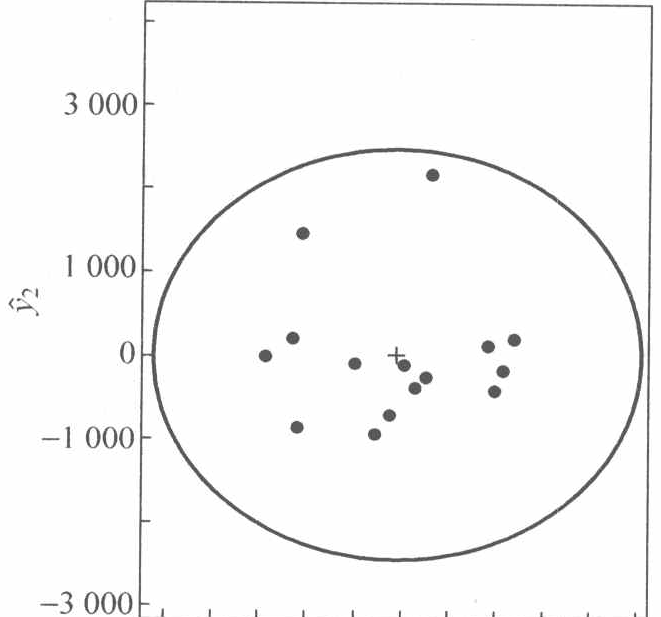
\includegraphics[width=56.0mm]{figs/fig_pg371_1.png}
\phantomsection\label{fig:8.9}\mvcap{图 8.9\quad 未来加班时间的前两个主成分的 99\%椭圆形式图}
\end{mvfigure}

在化学和制药行业的多元控制的某些应用中, 随时监控的变量超过 100. 这些变量既包括质量变量也包括数字化过程变量. 典型情况是, 与前几个主成分正交的空间, 有大于 100 的维数, 而某

%% ===== pg-372 =====

% ---- pg-372 （书页 360） ----

些特征值却很小. 为避免用很小的特征值去除小的平方主成分引起的困难, 已经成功地采用了另一种构造控制图的方法(见文献[13]). 该方法的实施步骤如下.

对各个稳定的观测值, 取它的未曾解释的成分的平方和
\[
d_{Uj}^2=(\mathbf{x}_j-\bar{\mathbf{x}}-\hat{y}_{j1}\hat{\mathbf{e}}_1-\hat{y}_{j2}\hat{\mathbf{e}}_2)'(\mathbf{x}_j-\bar{\mathbf{x}}-\hat{y}_{j1}\hat{\mathbf{e}}_1-\hat{y}_{j2}\hat{\mathbf{e}}_2)
\]
注意, 插入 $\hat{\mathbf{E}}\hat{\mathbf{E}}'=\mathbf{I}$, 我们也有
\[
d_{Uj}^2=(\mathbf{x}_j-\bar{\mathbf{x}}-\hat{y}_{j1}\hat{\mathbf{e}}_1-\hat{y}_{j2}\hat{\mathbf{e}}_2)'\hat{\mathbf{E}}\hat{\mathbf{E}}'(\mathbf{x}_j-\bar{\mathbf{x}}-\hat{y}_{j1}\hat{\mathbf{e}}_1-\hat{y}_{j2}\hat{\mathbf{e}}_2)=\sum_{k=3}^{p}\hat{y}_{jk}^2
\]
这正是所略去的主成分的平方和.

无论用哪一种形式, 画出 $(j,d_{Uj}^2)$ 曲线生成一张控制图. 图的下控制限是 0, 而上控制限由 $d_{Uj}^2$ 分布的近似来设定, 该分布是常数 $c$ 乘以自由度为 $v$ 的 $\chi^2$ 变量的分布.

对此 $\chi^2$ 近似, 常数 $c$ 和自由度 $v$ 的选取要与 $d_{Uj}^2$ $(j=1,2,\cdots,n)$ 的样本均值及方差相匹配. 特别地, 我们令
\[
\overline{d_U^2}=\frac{1}{n}\sum_{j=1}^{n}d_{Uj}^2=cv
\]
\[
s_{d^2}^2=\frac{1}{n-1}\sum_{j=1}^{n}(d_{Uj}^2-\overline{d_U^2})^2=2c^2v
\]
并确定
\[
c=\frac{s_{d^2}^2}{2\,\overline{d_U^2}}\qquad\text{和}\qquad v=2\,\frac{(\overline{d_U^2})^2}{s_{d^2}^2}
\]
上控制限就是 $c\chi_v^2(\alpha)$, 其中 $\alpha=0.05$ 或 $0.01$.

\section*{补充 8A\quad 样本主成分近似的几何意义}
\phantomsection\label{sec:8.7}

这个补充里我们将对基于前 $r$ 个样本主成分的数据近似, 提供一个解释. 对 $p$ 维散布图和 $n$ 维表示的解释, 要依赖下述代数结论. 我们考虑对形如 $\underset{(n\times p)}{\mathbf{A}}=[\mathbf{a}_1,\mathbf{a}_2,\cdots,\mathbf{a}_n]'$ 的矩阵以均值相关数据矩阵近似
\[
[\mathbf{x}_1-\bar{\mathbf{x}},\mathbf{x}_2-\bar{\mathbf{x}},\cdots,\mathbf{x}_n-\bar{\mathbf{x}}]'
\]
近似误差被量化为 $np$ 个平方误差之和
\phantomsection\label{eq:8A-1}
\begin{equation}
\sum_{j=1}^{n}(\mathbf{x}_j-\bar{\mathbf{x}}-\mathbf{a}_j)'(\mathbf{x}_j-\bar{\mathbf{x}}-\mathbf{a}_j)=\sum_{j=1}^{n}\sum_{i=1}^{p}(x_{ji}-\bar{x}_i-a_{ji})^2 \tag{8A-1}
\end{equation}

\mvthm{结论 8A.1}{令 $\underset{(n\times p)}{\mathbf{A}}$ 是任一矩阵, 秩$(\mathbf{A})\leqslant r<\min(p,n)$. 令 $\hat{\mathbf{E}}_r=[\hat{\mathbf{e}}_1,\hat{\mathbf{e}}_2,\cdots,\hat{\mathbf{e}}_r]$, 其中 $\hat{\mathbf{e}}_i$ 是 $\mathbf{S}$ 的第 $i$ 个特征向量. 选择}
\[
\hat{\mathbf{A}}=\begin{bmatrix}(\mathbf{x}_1-\bar{\mathbf{x}})'\\(\mathbf{x}_2-\bar{\mathbf{x}})'\\\vdots\\(\mathbf{x}_n-\bar{\mathbf{x}})'\end{bmatrix}\hat{\mathbf{E}}_r\hat{\mathbf{E}}_r'=[\hat{\mathbf{y}}_1,\hat{\mathbf{y}}_2,\cdots,\hat{\mathbf{y}}_r]\hat{\mathbf{E}}_r'
\]
使\hyperref[eq:8A-1]{式(8A-1)}中的近似平方和误差最小化, 故其转置 $\hat{\mathbf{A}}'$ 的第 $j$ 列为
\[
\hat{\mathbf{a}}_j=\hat{y}_{j1}\hat{\mathbf{e}}_1+\hat{y}_{j2}\hat{\mathbf{e}}_2+\cdots+\hat{y}_{jr}\hat{\mathbf{e}}_r
\]

%% ===== pg-373 =====

% ---- pg-373 （书页 361） ----

其中
\[
[\hat{y}_{j1},\hat{y}_{j2},\cdots,\hat{y}_{jr}]'=[\hat{\mathbf{e}}_1'(\mathbf{x}_j-\bar{\mathbf{x}}),\hat{\mathbf{e}}_2'(\mathbf{x}_j-\bar{\mathbf{x}}),\cdots,\hat{\mathbf{e}}_r'(\mathbf{x}_j-\bar{\mathbf{x}})]'
\]
是前 $r$ 个样本主成分对第 $j$ 个单元的值. 其次,
\[
\sum_{j=1}^{n}(\mathbf{x}_j-\bar{\mathbf{x}}-\hat{\mathbf{a}}_j)'(\mathbf{x}_j-\bar{\mathbf{x}}-\hat{\mathbf{a}}_j)=(n-1)(\hat{\lambda}_{r+1}+\cdots+\hat{\lambda}_p)
\]
其中 $\hat{\lambda}_{r+1}\geqslant\cdots\geqslant\hat{\lambda}_p$ 是 $\mathbf{S}$ 最小的一些特征值.

\noindent\textbf{证明}\quad 首先考虑任一矩阵 $\mathbf{A}$, 其转置 $\mathbf{A}'$ 的列 $\mathbf{a}_j$ 是固定一组 $r$ 个相互垂直向量 $\mathbf{u}_1,\mathbf{u}_2,\cdots,\mathbf{u}_r$ 的线性组合, 使 $\mathbf{U}=[\mathbf{u}_1,\mathbf{u}_2,\cdots,\mathbf{u}_r]$ 满足 $\mathbf{U}'\mathbf{U}=\mathbf{I}$. 对固定的 $\mathbf{U}$, $\mathbf{x}_j-\bar{\mathbf{x}}$ 在 $\mathbf{u}_1,\mathbf{u}_2,\cdots,\mathbf{u}_r$ 形成的空间的投影(见结论 2A.3)或者
\[
(\mathbf{x}_j-\bar{\mathbf{x}})'\mathbf{u}_1\mathbf{u}_1+(\mathbf{x}_j-\bar{\mathbf{x}})'\mathbf{u}_2\mathbf{u}_2+\cdots+(\mathbf{x}_j-\bar{\mathbf{x}})'\mathbf{u}_r\mathbf{u}_r,
\]
\phantomsection\label{eq:8A-2}
\begin{equation}
=[\mathbf{u}_1,\mathbf{u}_2,\cdots,\mathbf{u}_r]\begin{bmatrix}\mathbf{u}_1'(\mathbf{x}_j-\bar{\mathbf{x}})\\\mathbf{u}_2'(\mathbf{x}_j-\bar{\mathbf{x}})\\\vdots\\\mathbf{u}_r'(\mathbf{x}_j-\bar{\mathbf{x}})\end{bmatrix}=\mathbf{U}\mathbf{U}'(\mathbf{x}_j-\bar{\mathbf{x}}) \tag{8A-2}
\end{equation}
是它的最佳近似. 这是因为, 对任一向量 $\mathbf{b}_j$,
\[
\begin{aligned}
\mathbf{x}_j-\bar{\mathbf{x}}-\mathbf{U}\mathbf{b}_j&=\mathbf{x}_j-\bar{\mathbf{x}}-\mathbf{U}\mathbf{U}'(\mathbf{x}_j-\bar{\mathbf{x}})+\mathbf{U}\mathbf{U}'(\mathbf{x}_j-\bar{\mathbf{x}})-\mathbf{U}\mathbf{b}_j\\
&=(\mathbf{I}-\mathbf{U}\mathbf{U}')(\mathbf{x}_j-\bar{\mathbf{x}})+\mathbf{U}(\mathbf{U}'(\mathbf{x}_j-\bar{\mathbf{x}})-\mathbf{b}_j)
\end{aligned}
\]
因此误差平方和为
\[
\begin{aligned}
(\mathbf{x}_j-\bar{\mathbf{x}}-\mathbf{U}\mathbf{b}_j)'(\mathbf{x}_j-\bar{\mathbf{x}}-\mathbf{U}\mathbf{b}_j)&=(\mathbf{x}_j-\bar{\mathbf{x}})'(\mathbf{I}-\mathbf{U}\mathbf{U}')(\mathbf{x}_j-\bar{\mathbf{x}})+0\\
&\quad+(\mathbf{U}'(\mathbf{x}_j-\bar{\mathbf{x}})-\mathbf{b}_j)'(\mathbf{U}'(\mathbf{x}_j-\bar{\mathbf{x}})-\mathbf{b}_j)
\end{aligned}
\]
其中交叉乘积因 $(\mathbf{I}-\mathbf{U}\mathbf{U}')\mathbf{U}=\mathbf{U}-\mathbf{U}\mathbf{U}'\mathbf{U}=\mathbf{U}-\mathbf{U}=\mathbf{0}$ 而消失了. 最后一项是正的, 除非选 $\mathbf{b}_j$ 使 $\mathbf{b}_j=\mathbf{U}'(\mathbf{x}_j-\bar{\mathbf{x}})$, 且 $\mathbf{U}\mathbf{b}_j=\mathbf{U}\mathbf{U}'(\mathbf{x}_j-\bar{\mathbf{x}})$ 是 $(\mathbf{x}_j-\bar{\mathbf{x}})$ 在平面上的投影.

进而, 由于选 $\mathbf{a}_j=\mathbf{U}\mathbf{b}_j=\mathbf{U}\mathbf{U}'(\mathbf{x}_j-\bar{\mathbf{x}})$, \hyperref[eq:8A-1]{式(8A-1)}变为
\phantomsection\label{eq:8A-3}
\begin{equation}
\begin{aligned}
&\sum_{j=1}^{n}(\mathbf{x}_j-\bar{\mathbf{x}}-\mathbf{U}\mathbf{U}'(\mathbf{x}_j-\bar{\mathbf{x}}))'(\mathbf{x}_j-\bar{\mathbf{x}}-\mathbf{U}\mathbf{U}'(\mathbf{x}_j-\bar{\mathbf{x}}))\\
&\quad=\sum_{j=1}^{n}(\mathbf{x}_j-\bar{\mathbf{x}})'(\mathbf{I}-\mathbf{U}\mathbf{U}')(\mathbf{x}_j-\bar{\mathbf{x}})\\
&\quad=\sum_{j=1}^{n}(\mathbf{x}_j-\bar{\mathbf{x}})'(\mathbf{x}_j-\bar{\mathbf{x}})-\sum_{j=1}^{n}(\mathbf{x}_j-\bar{\mathbf{x}})'\mathbf{U}\mathbf{U}'(\mathbf{x}_j-\bar{\mathbf{x}})
\end{aligned}
\tag{8A-3}
\end{equation}
现在我们可以将\hyperref[eq:8A-3]{式(8A-3)}中最后一项最大化从而使误差在 $\mathbf{U}$ 上最小. 由迹的性质(见结论 2A.12),
\phantomsection\label{eq:8A-4}
\begin{equation}
\begin{aligned}
\sum_{j=1}^{n}(\mathbf{x}_j-\bar{\mathbf{x}})'\mathbf{U}\mathbf{U}'(\mathbf{x}_j-\bar{\mathbf{x}})&=\sum_{j=1}^{n}\mathrm{tr}[(\mathbf{x}_j-\bar{\mathbf{x}})'\mathbf{U}\mathbf{U}'(\mathbf{x}_j-\bar{\mathbf{x}})]\\
&=\sum_{j=1}^{n}\mathrm{tr}[\mathbf{U}\mathbf{U}'(\mathbf{x}_j-\bar{\mathbf{x}})(\mathbf{x}_j-\bar{\mathbf{x}})']\\
&=(n-1)\mathrm{tr}[\mathbf{U}\mathbf{U}'\mathbf{S}]=(n-1)\mathrm{tr}[\mathbf{U}'\mathbf{S}\mathbf{U}]
\end{aligned}
\tag{8A-4}
\end{equation}
也即 $\mathbf{U}$ 的最佳选择使 $\mathbf{U}'\mathbf{S}\mathbf{U}$ 对角元之和最大. 从\hyperref[eq:8-19]{式(8-19)}, 选 $\mathbf{u}_1$ 使 $\mathbf{U}'\mathbf{S}\mathbf{U}$ 的第一个对角元

%% ===== pg-374 =====

% ---- pg-374 （书页 362） ----

$\mathbf{u}_1'\mathbf{S}\mathbf{u}_1$ 最大, 这给出 $\mathbf{u}_1=\hat{\mathbf{e}}_1$. 对垂直于 $\hat{\mathbf{e}}_1$ 的 $\mathbf{u}_2$, 用 $\hat{\mathbf{e}}_2$ 使 $\mathbf{u}_2'\mathbf{S}\mathbf{u}_2$ 最大. 继续下去, 我们找到 $\hat{\mathbf{U}}=[\hat{\mathbf{e}}_1,\hat{\mathbf{e}}_2,\cdots,\hat{\mathbf{e}}_r]=\hat{\mathbf{E}}_r$ 及 $\hat{\mathbf{A}}=\hat{\mathbf{E}}_r\hat{\mathbf{E}}_r'[\mathbf{x}_1-\bar{\mathbf{x}},\mathbf{x}_2-\bar{\mathbf{x}},\cdots,\mathbf{x}_n-\bar{\mathbf{x}}]$, 这正如我们所断言的. \hfill$\blacksquare$

由于这一选取, $\hat{\mathbf{U}}'\mathbf{S}\hat{\mathbf{U}}$ 的第 $i$ 个对角元是 $\hat{\mathbf{e}}_i'\mathbf{S}\hat{\mathbf{e}}_i=\hat{\mathbf{e}}_i'(\hat{\lambda}_i\hat{\mathbf{e}}_i)=\hat{\lambda}_i$, 故 $\mathrm{tr}[\hat{\mathbf{U}}'\mathbf{S}\hat{\mathbf{U}}]=\hat{\lambda}_1+\hat{\lambda}_2+\cdots+\hat{\lambda}_r$. 同样地还有 $\sum_{j=1}^{n}(\mathbf{x}_j-\bar{\mathbf{x}})'(\mathbf{x}_j-\bar{\mathbf{x}})=\mathrm{tr}\left[\sum_{j=1}^{n}(\mathbf{x}_j-\bar{\mathbf{x}})(\mathbf{x}_j-\bar{\mathbf{x}})'\right]=(n-1)\mathrm{tr}(\mathbf{S})=(n-1)(\hat{\lambda}_1+\hat{\lambda}_2+\cdots+\hat{\lambda}_p)$. 在\hyperref[eq:8A-3]{式(8A-3)}中, 令 $\mathbf{U}=\hat{\mathbf{U}}$ 得到误差的界. \hfill$\blacksquare$

\mvsub{$p$ 维几何学解释}

几何学解释涉及确定对 $p$ 维散布图的最佳近似平面. 此平面通过原点, 由 $\mathbf{u}_1,\mathbf{u}_2,\cdots,\mathbf{u}_r$ 决定, 且由满足
\[
\mathbf{x}=b_1\mathbf{u}_1+b_2\mathbf{u}_2+\cdots+b_r\mathbf{u}_r=\mathbf{U}\mathbf{b},\quad \text{对某个 } \mathbf{b}
\]
的所有点 $\mathbf{x}$ 组成, 作变换使它通过 $\mathbf{a}$ 之后, 此平面对某个 $\mathbf{b}$ 变成 $\mathbf{a}+\mathbf{U}\mathbf{b}$.

我们要选此 $r$ 维平面 $\mathbf{a}+\mathbf{U}\mathbf{b}$ 使观测值 $\mathbf{x}_j$ 与该平面之间的平方距离和 $\sum_{j=1}^{n}d_j^2$ 达到最小. 若 $\mathbf{x}_j$ 用 $\mathbf{a}+\mathbf{U}\mathbf{b}_j$(满足 $\sum_{j=1}^{n}\mathbf{b}_j=\mathbf{0}$)来近似\footnote{若 $\sum_{j=1}^{n}\mathbf{b}_j=n\bar{\mathbf{b}}\neq\mathbf{0}$, 就用 $\mathbf{a}+\mathbf{U}\mathbf{b}_j=(\mathbf{a}+\mathbf{U}\bar{\mathbf{b}})+\mathbf{U}(\mathbf{b}_j-\bar{\mathbf{b}})=\mathbf{a}^*+\mathbf{U}\mathbf{b}_j^*$.}, 则由于矩阵 $[\mathbf{U}\mathbf{b}_1,\cdots,\mathbf{U}\mathbf{b}_n]=\mathbf{A}'$ 有秩$(\mathbf{A})\leqslant r$, 故根据结论 8A.1 有
\[
\begin{aligned}
&\sum_{j=1}^{n}(\mathbf{x}_j-\mathbf{a}-\mathbf{U}\mathbf{b}_j)'(\mathbf{x}_j-\mathbf{a}-\mathbf{U}\mathbf{b}_j)\\
&\quad=\sum_{j=1}^{n}(\mathbf{x}_j-\bar{\mathbf{x}}-\mathbf{U}\mathbf{b}_j+\bar{\mathbf{x}}-\mathbf{a})'(\mathbf{x}_j-\bar{\mathbf{x}}-\mathbf{U}\mathbf{b}_j+\bar{\mathbf{x}}-\mathbf{a})\\
&\quad=\sum_{j=1}^{n}(\mathbf{x}_j-\bar{\mathbf{x}}-\mathbf{U}\mathbf{b}_j)'(\mathbf{x}_j-\bar{\mathbf{x}}-\mathbf{U}\mathbf{b}_j)+n(\bar{\mathbf{x}}-\mathbf{a})'(\bar{\mathbf{x}}-\mathbf{a})\\
&\quad\geqslant\sum_{j=1}^{n}(\mathbf{x}_j-\bar{\mathbf{x}}-\hat{\mathbf{E}}_r\hat{\mathbf{E}}_r'(\mathbf{x}_j-\bar{\mathbf{x}}))'(\mathbf{x}_j-\bar{\mathbf{x}}-\hat{\mathbf{E}}_r\hat{\mathbf{E}}_r'(\mathbf{x}_j-\bar{\mathbf{x}}))
\end{aligned}
\]
取 $\mathbf{a}=\bar{\mathbf{x}}$ 达到下界, 故此平面通过样本均值, 此平面由 $\hat{\mathbf{e}}_1,\hat{\mathbf{e}}_2,\cdots,\hat{\mathbf{e}}_r$ 决定, $\hat{\mathbf{e}}_k$ 的系数为 $\hat{\mathbf{e}}_k'(\mathbf{x}_j-\bar{\mathbf{x}})=\hat{y}_{jk}$, 它是在第 $j$ 个观测值估计的第 $k$ 个样本主成分.

\begin{mvfigure}
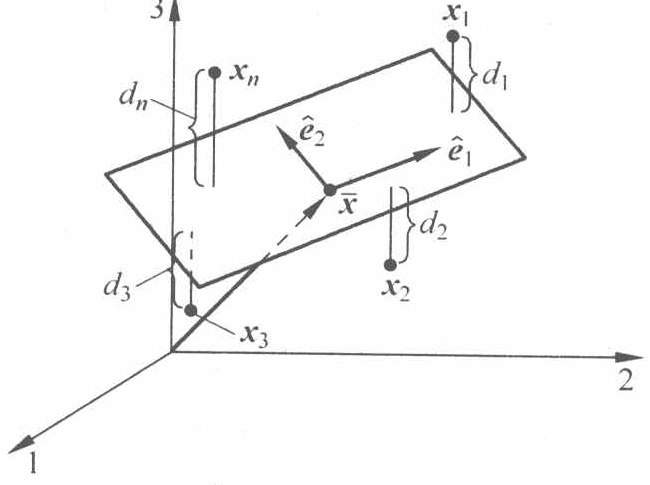
\includegraphics[width=55.1mm]{figs/fig_pg374_1.png}
\phantomsection\label{fig:8.10}\mvcap{图 8.10\quad 用 $\sum_{j=1}^{n}d_j^2$ 的最小化逼近散布图的 $r=2$ 维平面}
\end{mvfigure}

样本主成分的近似平面解释, 由\hyperref[fig:8.10]{图 8.10} 表示.

可以给出另一个替代的解释. 置平面穿过 $\bar{\mathbf{x}}$ 并稍作移动使得观测值在平面的投影达到最大伸长. 从\hyperref[eq:8A-2]{式(8A-2)}, 变差 $\mathbf{x}_j-\bar{\mathbf{x}}$ 在平面 $\mathbf{U}\mathbf{b}$ 的投影是 $\mathbf{v}_j=\mathbf{U}\mathbf{U}'(\mathbf{x}_j-\bar{\mathbf{x}})$. 现在, $\bar{\mathbf{v}}=\mathbf{0}$ 且投影变差的平方长度之和为

%% ===== pg-375 =====

% ---- pg-375 （书页 363） ----

\[
\sum_{j=1}^{n}\mathbf{v}_j'\mathbf{v}_j=\sum_{j=1}^{n}(\mathbf{x}_j-\bar{\mathbf{x}})'\mathbf{U}\mathbf{U}'(\mathbf{x}_j-\bar{\mathbf{x}})=(n-1)\mathrm{tr}[\mathbf{U}'\mathbf{S}\mathbf{U}]
\]
由 $\mathbf{U}=\hat{\mathbf{E}}$ 得到最大. 由于 $\bar{\mathbf{v}}=\mathbf{0}$, 也还有
\[
(n-1)\mathbf{S}_{\mathbf{v}}=\sum_{j=1}^{n}(\mathbf{v}_j-\bar{\mathbf{v}})(\mathbf{v}_j-\bar{\mathbf{v}})'=\sum_{j=1}^{n}\mathbf{v}_j\mathbf{v}_j'
\]
且此平面也使总方差达到
\[
\mathrm{tr}(\mathbf{S}_{\mathbf{v}})=\frac{1}{(n-1)}\mathrm{tr}\left[\sum_{j=1}^{n}\mathbf{v}_j\mathbf{v}_j'\right]=\frac{1}{(n-1)}\mathrm{tr}\left[\sum_{j=1}^{n}\mathbf{v}_j'\mathbf{v}_j\right]
\]
最大.

\mvsub{$n$ 维几何学解释}

我们现在来考虑, 按列用 $\mathbf{A}$ 逼近均值中心化数据矩阵. 对 $r=1$, 第 $i$ 列 $[x_{1i}-\bar{x}_i,x_{2i}-\bar{x}_i,\cdots,x_{ni}-\bar{x}_i]'$ 由一个固定向量 $\mathbf{b}=[b_1,b_2,\cdots,b_n]'$ 的乘积 $c_i\mathbf{b}'$ 来近似. 此近似误差的平方长度为
\[
L_i^2=\sum_{j=1}^{n}(x_{ji}-\bar{x}_i-c_ib_j)^2
\]
考虑到矩阵 $\mathbf{A}_{(n\times p)}$ 秩为 1, 我们从结论 8A.1 得出:
\[
\hat{\mathbf{A}}=\begin{bmatrix}\hat{\mathbf{e}}_1\hat{\mathbf{e}}_1'(\mathbf{x}_1-\bar{\mathbf{x}})\\ \hat{\mathbf{e}}_1\hat{\mathbf{e}}_1'(\mathbf{x}_2-\bar{\mathbf{x}})\\ \vdots\\ \hat{\mathbf{e}}_1\hat{\mathbf{e}}_1'(\mathbf{x}_n-\bar{\mathbf{x}})\end{bmatrix}=\begin{bmatrix}\hat{y}_{11}\\ \hat{y}_{21}\\ \vdots\\ \hat{y}_{n1}\end{bmatrix}\hat{\mathbf{e}}_1'
\]
将平方长度之和 $\sum_{i=1}^{p}L_i^2$ 最小化. 也即, 第一主成分值的向量决定最佳方向. 在\hyperref[fig:8.11]{图 8.11}(a) 中这一点得到了说明. 注意, 较长的变差向量(更大的 $s_{ii}$)对 $\sum_{i=1}^{p}L_i^2$ 的最小化影响最大.

如果先将变量标准化, 则对所有的变量, 得到的向量 $\left[(x_{1i}-\bar{x}_i)/\sqrt{s_{ii}},(x_{2i}-\bar{x}_i)/\sqrt{s_{ii}},\cdots,(x_{ni}-\bar{x}_i)/\sqrt{s_{ii}}\right]'$ 长度为 $n-1$, 且每个向量对方向选择的影响相等 [见\hyperref[fig:8.11]{图 8.11}(b)].

在两种情况下, 在 $n$ 维空间中旋转 $\mathbf{b}$ 使平方距离之和 $\sum_{i=1}^{p}L_i^2$ 最小, 其中 $L_i$ 是 $[x_{1i}-\bar{x}_i,x_{2i}-\bar{x}_i,\cdots$

\begin{mvfigure}
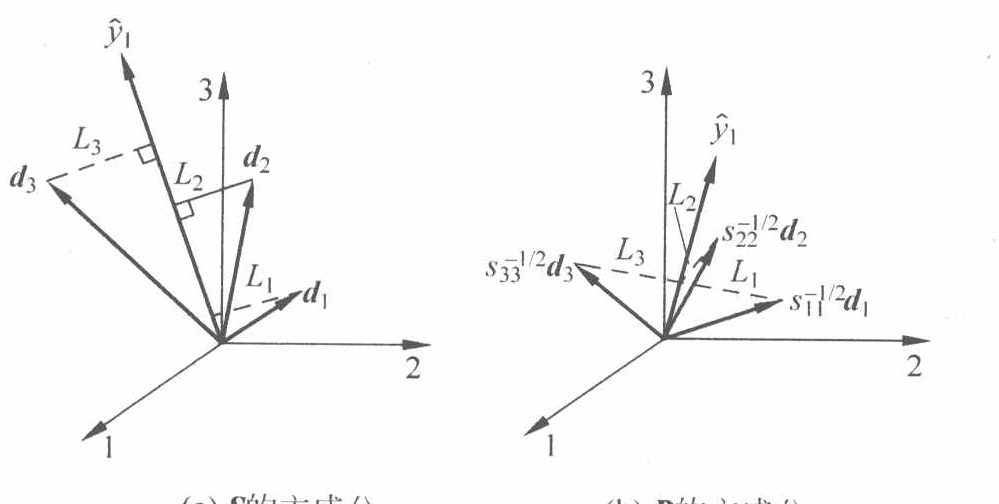
\includegraphics[width=84.5mm]{figs/fig_pg375_1.png}
\phantomsection\label{fig:8.11}\mvcap{图 8.11\quad 第一样本主成分 $\hat{y}_1$ 使离差向量 $\mathbf{d}_i=[x_{1i}-\bar{x}_i,x_{2i}-\bar{x}_i,\cdots,x_{ni}-\bar{x}_i]'$ 到直线的距离平方之和最小化}
\end{mvfigure}

%% ===== pg-376 =====

% ---- pg-376 （书页 364） ----

$x_i,\cdots,x_{ni}-\bar{x}_i]'$ 与其在由 $\mathbf{b}$ 决定的直线上的投影之间的平方距离. 第二主成分使在与第一次选定向量垂直的所有向量中上述平方距离之和最小.

\mvsub{练习}

\noindent 8.1\quad 试确定下述协方差矩阵的总体主成分 $Y_1$ 和 $Y_2$
\[
\boldsymbol{\Sigma}=\begin{bmatrix}5&2\\2&2\end{bmatrix}
\]
并计算总体总方差中第一主成分所解释的比例.

\noindent 8.2\quad 把练习 8.1 中的协方差矩阵换为相关系数矩阵 $\boldsymbol{\rho}$.

(a) 试确定来自 $\boldsymbol{\rho}$ 的主成分 $Y_1$ 和 $Y_2$, 并计算总体总方差中用 $Y_1$ 解释的比例.

(b) 将 (a) 中求得的成分与练习 8.1 中得到的作比较. 它们相同吗? 应该相同吗?

(c) 计算相关系数 $\rho_{Y_1,Z_1},\rho_{Y_1,Z_2}$ 和 $\rho_{Y_2,Z_1}$.

\noindent 8.3\quad 令
\[
\boldsymbol{\Sigma}=\begin{bmatrix}2&0&0\\0&4&0\\0&0&4\end{bmatrix}
\]
试确定主成分 $Y_1,Y_2$ 和 $Y_3$. 对彼此相等的特征值所对应的那些特征向量(及主成分)你能说些什么?

\noindent 8.4\quad 求主成分及总体总方差中用每一个主成分解释的比例, 此时协方差矩阵为
\[
\boldsymbol{\Sigma}=\begin{bmatrix}\sigma^2&\sigma^2\rho&0\\\sigma^2\rho&\sigma^2&\sigma^2\rho\\0&\sigma^2\rho&\sigma^2\end{bmatrix},\quad -\frac{1}{\sqrt{2}}<\rho<\frac{1}{\sqrt{2}}
\]

\noindent 8.5\quad (a) 求相关系数矩阵 $\boldsymbol{\rho}$ 的特征值,
\[
\boldsymbol{\rho}=\begin{bmatrix}1&\rho&\rho\\\rho&1&\rho\\\rho&\rho&1\end{bmatrix}
\]
你的结果与\hyperref[eq:8-16]{式(8-16)}和\hyperref[eq:8-17]{式(8-17)}相一致吗?

(b) 验证\hyperref[eq:8-15]{式(8-15)}给出的 $p\times p$ 矩阵 $\boldsymbol{\rho}$ 的特征值-特征向量对.

\noindent 8.6\quad 对美国 10 家最大的工业公司 $x_1=$ 销售额, $x_2=$ 利润的数据列于第 1 章的练习 1.4. 由例 4.12,
\[
\bar{\mathbf{x}}=\begin{bmatrix}155.60\\14.70\end{bmatrix},\quad \mathbf{S}=\begin{bmatrix}7\,476.45&303.62\\303.62&26.19\end{bmatrix}
\]

(a) 求样本主成分及这些数据的方差(你可能需要用到二次型去解出 $\mathbf{S}$ 的特征值).

(b) 求样本总方差中用 $\hat{y}_1$ 解释的比例.

(c) 画出常数密度椭圆 $(\mathbf{x}-\bar{\mathbf{x}})'\mathbf{S}^{-1}(\mathbf{x}-\bar{\mathbf{x}})=1.4$, 并在图上标出主成分 $\hat{y}_1$ 和 $\hat{y}_2$.

(d) 计算相关系数 $r_{\hat{y}_1,x_k},k=1,2$. 如果可以, 你能对第一主成分作什么解释?

\noindent 8.7\quad 将练习 8.6 中的协方差矩阵 $\mathbf{S}$ 换成样本相关系数矩阵 $\mathbf{R}$.

(a) 求样本主成分 $\hat{y}_1,\hat{y}_2$ 及它们的方差.

%% ===== pg-377 =====

% ---- pg-377 （书页 365） ----

(b) 计算全部样本方差中由 $\hat{y}_1$ 解释的比例.

(c) 计算相关系数 $r_{\hat{y}_1,z_k},k=1,2$. 解释 $\hat{y}_1$.

(d) 比较由 (a) 得到的成分和由练习 8.6(a) 求得的成分. 已知列于练习 1.4 的原始数据, 你认为由样本协方差矩阵或样本相关系数矩阵求主成分, 哪个会更好些? 试说明之.

\noindent 8.8\quad 利用例 8.5 的结果:

(a) 计算相关系数 $r_{\hat{y}_i,z_k},i=1,2$ 和 $k=1,2,\cdots,5$. 这些相关系数是否加强了对前两个成分的解释? 试说明之.

(b) 在 $5\%$ 显著性水平, 检验假设
\[
H_0:\boldsymbol{\rho}=\boldsymbol{\rho}_0=\begin{bmatrix}1&\rho&\rho&\rho&\rho\\ \rho&1&\rho&\rho&\rho\\ \rho&\rho&1&\rho&\rho\\ \rho&\rho&\rho&1&\rho\\ \rho&\rho&\rho&\rho&1\end{bmatrix}
\]
\[
H_1:\boldsymbol{\rho}\neq\boldsymbol{\rho}_0
\]
列出在完成检验时需要的所有假定.

\noindent 8.9\quad (所有变量相互独立的检验.)

(a) 考虑正态理论似然比检验 $H_0:\boldsymbol{\Sigma}$ 为对角阵
\[
\begin{bmatrix}\sigma_{11}&0&\cdots&0\\ 0&\sigma_{22}&\cdots&0\\ \vdots&\vdots&\ddots&\vdots\\ 0&0&\cdots&\sigma_{pp}\end{bmatrix},\quad \sigma_{ii}>0
\]
证明检验为: 若
\[
\Lambda=\frac{|\mathbf{S}|^{n/2}}{\prod_{i=1}^{p}s_{ii}^{n/2}}=|\mathbf{R}|^{n/2}<c
\]
则拒绝 $H_0$.

对于大样本, $-2\ln\Lambda$ 近似 $\chi^2_{p(p-1)/2}$ 分布. 巴特利特[3]建议检验统计量以 $-2[1-(2p+11)/6n]\ln\Lambda$ 取代 $-2\ln\Lambda$. 这得出一个改善的 $\chi^2$ 近似. 大样本的 $\alpha$ 临界点为 $\chi^2_{p(p-1)/2}(\alpha)$. 注意, 检验 $\boldsymbol{\Sigma}=\boldsymbol{\Sigma}_0$ 与检验 $\boldsymbol{\rho}=\mathbf{I}$ 是一样的.

(b) 证明对似然比检验 $H_0:\boldsymbol{\Sigma}=\sigma^2\mathbf{I}$, 当下式成立则拒绝 $H_0$
\[
\Lambda=\frac{|\mathbf{S}|^{n/2}}{(\mathrm{tr}(\mathbf{S})/p)^{np/2}}=\left[\frac{\prod_{i=1}^{p}\hat{\lambda}_i}{\left(\frac{1}{p}\sum_{i=1}^{p}\hat{\lambda}_i\right)^p}\right]^{n/2}=\left[\frac{\text{几何均值 }\hat{\lambda}_i}{\text{算术均值 }\hat{\lambda}_i}\right]^{np/2}<c
\]
对大容量样本, 巴特利特[3]认为 $-2[1-(2p^2+p+2)/6pn]\ln\Lambda$ 近似服从 $\chi^2_{(p+2)(p-1)/2}$. 因此, 该大样本的 $\alpha$ 临界点是 $\chi^2_{(p+2)(p-1)/2}(\alpha)$. 因为当 $\boldsymbol{\Sigma}=\sigma^2\mathbf{I}$ 时, 常数密度的轮廓线是球面, 因此这个检验称为球性检验.

提示:

(a) $\max_{\boldsymbol{\mu},\boldsymbol{\Sigma}}L(\boldsymbol{\mu},\boldsymbol{\Sigma})$ 由\hyperref[eq:5-10]{式(5-10)}给出, 并且 $\max_{\boldsymbol{\mu}}L(\boldsymbol{\mu},\boldsymbol{\Sigma}_0)$ 是单变量似然函数的积:

%% ===== pg-378 =====

% ---- pg-378 （书页 366） ----

\[
\max_{\mu_i,\sigma_{ii}}(2\pi)^{-n/2}\sigma_{ii}^{-n/2}\exp\left[-\sum_{j=1}^{n}(x_{ji}-\mu_i)^2/2\sigma_{ii}\right],\quad \text{所以, } \hat{\mu}_i=n^{-1}\sum_{j=1}^{n}x_{ji}
\]
且 $\hat{\sigma}_{ii}=(1/n)\sum_{j=1}^{n}(x_{ji}-\bar{x}_i)^2$. 除数 $n$ 在 $\Lambda$ 中抵消, 故可用 $\mathbf{S}$.

(b) 在 $H_0$ 下验证 $\hat{\sigma}^2=\left[\sum_{j=1}^{n}(x_{j1}-\bar{x}_1)^2+\cdots+\sum_{j=1}^{n}(x_{jp}-\bar{x}_p)^2\right]/np$.

在统计量中去掉除数 $n$, 再验证仍然可用 $\mathbf{S}$. 利用结论 5.2 计算 $\hat{\chi}^2$ 的自由度.

\mvbold{以下练习需用计算机.}

\noindent 8.10\quad \hyperref[tab:8.4]{表 8.4} 给出在纽约股票交易所交易的五支股票的周回报率(见网页 www.prenhall.com/statistics 上的股票价格数据).

(a) 构造样本协方差矩阵 $\mathbf{S}$, 并求\hyperref[eq:8-20]{式(8-20)}的样本主成分. (注意, 样本均值向量 $\bar{\mathbf{x}}$ 已在例 8.5 中列出了.)

(b) 确定样本总方差中用前三个主成分解释的比例. 解释这些成分.

(c) 前三个总体成分 $Y_1,Y_2$ 和 $Y_3$ 的方差为 $\lambda_1,\lambda_2$ 和 $\lambda_3$, 构造它们的庞弗罗尼 $90\%$ 联合置信区间.

(d) 已知 (a)$\sim$(c) 的结果, 你认为要综合股票回报率数据, 在小于五维空间中是否可行? 试解释.

\begin{mvtable}
\phantomsection\label{tab:8.4}\mvtabcap{表 8.4\quad 股票价格数据(周回报率)}
\begin{longtable}{lrrrrr}\toprule
周 & JP Morgan & Citibank & Wells Fargo & Royal Dutch Shell & Exxon Mobil\\
\midrule
\endfirsthead
\multicolumn{6}{c}{\zihao{6}续表}\\
\toprule
周 & JP Morgan & Citibank & Wells Fargo & Royal Dutch Shell & Exxon Mobil\\
\midrule
\endhead
\bottomrule
\endlastfoot

1 & 0.013 03 & $-0.007$ 84 & $-0.003$ 19 & $-0.044$ 77 & 0.005 22\\
2 & 0.008 49 & 0.016 69 & $-0.006$ 21 & 0.01196 & 0.013 49\\
3 & $-0.017$ 92 & $-0.008$ 64 & 0.010 04 & 0 & $-0.006$ 14\\
4 & 0.021 56 & $-0.003$ 49 & 0.017 44 & $-0.028$ 59 & $-0.006$ 95\\
5 & 0.010 82 & 0.003 72 & $-0.010$ 13 & 0.029 19 & 0.040 98\\
6 & 0.010 17 & $-0.012$ 20 & $-0.008$ 38 & 0.013 71 & 0.002 99\\
7 & 0.011 13 & 0.028 00 & 0.008 07 & 0.030 54 & 0.003 23\\
8 & 0.048 48 & $-0.005$ 15 & 0.018 25 & 0.006 33 & 0.007 68\\
9 & $-0.034$ 49 & $-0.013$ 80 & $-0.008$ 05 & $-0.029$ 90 & $-0.010$ 81\\
10 & $-0.004$ 66 & 0.020 99 & $-0.006$ 08 & $-0.020$ 39 & $-0.012$ 67\\
$\vdots$ & $\vdots$ & $\vdots$ & $\vdots$ & $\vdots$ & $\vdots$\\
94 & 0.037 32 & 0.035 93 & 0.025 28 & 0.058 19 & 0.016 97\\
95 & 0.023 80 & 0.003 11 & $-0.006$ 88 & 0.012 25 & 0.028 17\\
96 & 0.025 68 & 0.052 53 & 0.040 70 & $-0.031$ 66 & $-0.018$ 85\\
97 & $-0.066$ 06 & 0.008 63 & 0.005 84 & 0.044 56 & 0.030 59\\
98 & 0.021 74 & 0.022 96 & 0.029 20 & 0.008 44 & 0.031 93\\
99 & 0.003 37 & $-0.015$ 31 & $-0.023$ 82 & $-0.001$ 67 & $-0.017$ 23\\
100 & 0.003 36 & 0.002 90 & $-0.003$ 05 & $-0.001$ 22 & $-0.009$ 70\\
101 & 0.017 01 & 0.009 51 & 0.018 20 & $-0.016$ 18 & $-0.007$ 56\\
102 & 0.010 39 & $-0.002$ 66 & 0.044 43 & 0.002 48 & $-0.016$ 45\\
103 & $-0.012$ 79 & $-0.014$ 37 & $-0.018$ 74 & $-0.004$ 98 & $-0.016$ 37\\
\end{longtable}
\end{mvtable}

%% ===== pg-379 =====

% ---- pg-379 （书页 367） ----

\noindent 8.11\quad 考虑\hyperref[tab:8.5]{表 8.5} 的人口普查数据. 对 $X_5=$ 家庭收入中位数的观察值, 用千美元计数而不用万美元. 也就是说, 将表中第 6 列的所有数字都乘以 10.

\begin{mvtable}
\phantomsection\label{tab:8.5}\mvtabcap{表 8.5\quad 人口调查数据}
\mvfit{%
\begin{tabular}{lccccc}
\toprule
区 & 总人口(千人) & 职业度(\%) & 16 岁以上就业率(\%) & 政府雇用率(\%) & 家庭收入中位数(10 万美元)\\
\midrule
1 & 2.67 & 5.71 & 69.02 & 30.3 & 1.48\\
2 & 2.25 & 4.37 & 72.98 & 43.3 & 1.44\\
3 & 3.12 & 10.27 & 64.94 & 32.0 & 2.11\\
4 & 5.14 & 7.44 & 71.29 & 24.5 & 1.85\\
5 & 5.54 & 9.25 & 74.94 & 31.0 & 2.23\\
6 & 5.04 & 4.84 & 53.61 & 48.2 & 1.60\\
7 & 3.14 & 4.82 & 67.00 & 37.6 & 1.52\\
8 & 2.43 & 2.40 & 67.20 & 36.8 & 1.40\\
9 & 5.38 & 4.30 & 83.03 & 19.7 & 2.07\\
10 & 7.34 & 2.73 & 72.60 & 24.5 & 1.42\\
$\vdots$ & $\vdots$ & $\vdots$ & $\vdots$ & $\vdots$ & $\vdots$\\
52 & 7.25 & 1.16 & 78.52 & 23.6 & 1.50\\
53 & 5.44 & 2.93 & 73.59 & 22.3 & 1.65\\
54 & 5.83 & 4.47 & 77.33 & 26.2 & 2.16\\
55 & 3.74 & 2.26 & 79.70 & 20.2 & 1.58\\
56 & 9.21 & 2.36 & 74.58 & 21.8 & 1.72\\
57 & 2.14 & 6.30 & 86.54 & 17.4 & 2.80\\
58 & 6.62 & 4.79 & 78.84 & 20.0 & 2.33\\
59 & 4.24 & 5.82 & 71.39 & 27.1 & 1.69\\
60 & 4.72 & 4.71 & 78.01 & 20.6 & 1.55\\
61 & 6.48 & 4.93 & 74.23 & 20.9 & 1.98\\
\bottomrule
\end{tabular}
}

{\small 注: 观测数据似乎有相关性, 即 61 个观测可能不构成随机样本. 全部数据可从 www.prenhall.com/statistics 得到.}
\end{mvtable}

(a) 构造人口普查数据的样本协方差矩阵 $\mathbf{S}$, 此时 $X_5=$ 家庭收入中位数用千美元为单位计数. (注意, 这个协方差矩阵可由例 8.3 给出的协方差矩阵得到, 将其第 5 行和第 5 列的非对角元乘以 10 并将对角元 $s_{55}$ 乘以 100 即可, 为什么呢?)

(b) 求特征值-特征向量对及(a)中协方差矩阵的前两个样本主成分.

(c) 计算总方差中用(b)求得的前两个主成分解释的比例, 求相关系数 $r_{\hat{y}_i,x_k}$. 如果可能的话, 解释这些成分, 并将所得结果与例 8.3 的结果进行比较. 计数尺度上的变化对主成分有什么影响?

\noindent 8.12\quad 考虑列于\hyperref[tab:1.5]{表 1.5} 的空气污染数据, 如果可能请用小于 $p=7$ 维来综合这些数据. 用协方差矩阵 $\mathbf{S}$ 和相关系数矩阵 $\mathbf{R}$ 对这些数据做主成分分析, 你能从中学到什么? 选择哪个矩阵作分析有不同吗? 这些数据可由三维甚至更少的维数来综合吗? 你能解释这些主成分吗?

\noindent 8.13\quad 放射疗法数据在\hyperref[tab:1.7]{表 1.7} 中, 对 $p=6$ 个代表病人对放射疗法的反应的变量有 $n=98$ 次观察值.

(a) 求这些数据的协方差矩阵 $\mathbf{S}$ 及相关系数矩阵 $\mathbf{R}$.

(b) 挑选一个矩阵 $\mathbf{S}$ 或 $\mathbf{R}$(证明你的选择合理)然后求特征值和特征向量. 按从大到小的

%% ===== pg-380 =====

% ---- pg-380 （书页 368） ----

顺序, 列表表示每个特征值对样本总方差的贡献百分比.

(c) 已知(b)的结果, 确定重要样本主成分的个数, 若用单一的反应指标成分来综合放射疗法数据是否可行? 请说明.

(d) 列表写出每一个你想保留的主成分与原始数据间的相关系数. 如果可能, 解释这些成分.

\noindent 8.14\quad 用例 5.2 的汗液数据的样本协方差矩阵作主成分分析, 作每个重要主成分的 Q-Q 散点图, 有可疑的观察值吗? 试说明.

\noindent 8.15\quad 在例 8.6 中讨论过的生育后体重的 4 个样本标准差为
\[
\sqrt{s_{11}}=32.990\,9,\quad \sqrt{s_{22}}=33.591\,8,\quad \sqrt{s_{33}}=36.553\,4,\quad \sqrt{s_{44}}=37.351\,7
\]
用这些数据和例 8.6 给定的相关系数, 构造样本协方差矩阵 $\mathbf{S}$, 用 $\mathbf{S}$ 作主成分分析.

\noindent 8.16\quad 20 世纪 90 年代, 在五年的时间里, 以威斯康星的 28 个湖上的渔民作为年度样本, 要求他们报告捕鱼花费的时间及捕到的各种类型的鱼的数量, 然后把他们反馈的信息转化成对下面几种鱼的每小时的捕捉率,
\[
\begin{array}{lll}
x_1=\text{蓝鳃鱼} & x_2=\text{黑刺盖太阳鱼} & x_3=\text{小嘴鲈鱼}\\
x_4=\text{大嘴鲈鱼} & x_5=\text{突眼鱼} & x_6=\text{北方狗鱼}
\end{array}
\]
估计的相关系数矩阵为
\[
\mathbf{R}=\begin{bmatrix}
1&0.491\,9&0.263\,6&0.465\,3&-0.227\,7&0.065\,2\\
0.491\,9&1&0.312\,7&0.350\,6&-0.191\,7&0.204\,5\\
0.263\,5&0.312\,7&1&0.410\,8&0.064\,7&0.249\,3\\
0.465\,3&0.350\,6&0.410\,8&1&-0.224\,9&0.229\,3\\
-0.227\,7&-0.191\,7&0.064\,7&-0.224\,9&1&-0.214\,4\\
0.065\,2&0.204\,5&0.249\,3&0.229\,3&-0.214\,4&1
\end{bmatrix}
\]
它是基于一个容量为 120 的样本(有少量数值丢失了).

同一个渔夫捕到的鱼都放在一起, 因此这些数据可以提供关于鱼群的一些迹象. 前四种鱼属于棘臀太阳鱼科, 这是数量最丰富的科. 突眼鱼则是最受欢迎的食用鱼.

(a) 论述棘臀太阳鱼科内 $x_1$ 至 $x_4$ 的相关系数模型, 突眼鱼与其他几种鱼是同一鱼群的吗?

(b) 仅用 $x_1$ 至 $x_4$ 作主成分分析, 解释你的结果.

(c) 用全部 6 个变量进行主成分分析. 解释得到的结果.

\noindent 8.17\quad 用\hyperref[tab:1.8]{表 1.8} 中的骨头所含矿物质的数据, 作 $\mathbf{S}$ 的主成分分析.

\noindent 8.18\quad 国家和地区的女子田径纪录数据列于\hyperref[tab:1.9]{表 1.9}.

(a) 求这些数据的样本相关系数矩阵 $\mathbf{R}$, 并求它的特征值和特征向量.

(b) 求标准化变量的前两个主成分. 列表表示标准化变量的相关系数, 并给出主成分及由这两个主成分解释的(标准化)样本总方差累积百分比.

(c) 解释(b)中求得的两个主成分(注意, 第一成分实质上是规范化的单位向量, 并且可以测量给定国家和地区的运动员的水平. 第二成分测量国家和地区在不同赛跑距离中的相对实力).

(d) 把国家和地区按它们在第一主成分的得分排列, 这种排列与你最初对不同国家和地区运动水平的看法相一致吗?

%% ===== pg-381 =====

% ---- pg-381 （书页 369） ----

\noindent 8.19\quad 参见练习 8.18, 用以米/秒为单位的速度代替原\hyperref[tab:1.9]{表 1.9} 中的国家和地区女子田径纪录, 注意, 800 米、1 500 米、3 000 米和马拉松的纪录是用分钟标示的. 马拉松是 26.2 英里或 42 195 米长. 用速度数据的协方差矩阵 $\mathbf{S}$ 作主成分分析, 与练习 8.18 的结果作比较. 你对成分的解释有不同吗? 若这些国家和地区的名次是以其第一主成分上的得分来排列的, 那么这个序列与练习 8.18 的有所不同吗? 为什么?

\noindent 8.20\quad \hyperref[tab:8.6]{表 8.6} 列出各国家和地区男子径赛记录的数据(又见网页 www. prenhall. com/statistics 上的国家男子径赛记录数据). 像练习 8.18 那样重复作一次主成分分析, 得到的结果是否与那些由女子数据得到的结果一致?

\begin{mvtable}
\phantomsection\label{tab:8.6}\mvtabcap{表 8.6\quad 男子径赛国家和地区纪录}
\begin{tabular}{lcccccccc}
\toprule
国家和地区 & 100m & 200m & 400m & 800m & 1 500m & 5 000m & 10 000m & 马拉松 \\
 & (s) & (s) & (s) & (min) & (min) & (min) & (min) & (min) \\
\midrule
阿根廷 & 10.23 & 20.37 & 46.18 & 1.77 & 3.68 & 13.33 & 27.65 & 129.57 \\
澳大利亚 & 9.93 & 20.06 & 44.38 & 1.74 & 3.53 & 12.93 & 27.53 & 127.51 \\
奥地利 & 10.15 & 20.45 & 45.80 & 1.77 & 3.58 & 13.26 & 27.72 & 132.22 \\
比利时 & 10.14 & 20.19 & 45.02 & 1.73 & 3.57 & 12.83 & 26.87 & 127.20 \\
百慕大 & 10.27 & 20.30 & 45.26 & 1.79 & 3.70 & 14.64 & 30.49 & 146.37 \\
巴西 & 10.00 & 19.89 & 44.29 & 1.70 & 3.57 & 13.48 & 28.13 & 126.05 \\
加拿大 & 9.84 & 20.17 & 44.72 & 1.75 & 3.53 & 13.23 & 27.60 & 130.09 \\
智利 & 10.10 & 20.15 & 45.92 & 1.76 & 3.65 & 13.39 & 28.09 & 132.19 \\
中国 & 10.17 & 20.42 & 45.25 & 1.77 & 3.61 & 13.42 & 28.17 & 129.18 \\
哥伦比亚 & 10.29 & 20.85 & 45.84 & 1.80 & 3.72 & 13.49 & 27.88 & 131.17 \\
库克群岛 & 10.97 & 22.46 & 51.40 & 1.94 & 4.24 & 16.70 & 35.38 & 171.26 \\
哥斯达黎加 & 10.32 & 20.96 & 46.42 & 1.87 & 3.84 & 13.75 & 28.81 & 133.23 \\
捷克 & 10.24 & 20.61 & 45.77 & 1.75 & 3.58 & 13.42 & 27.80 & 131.57 \\
丹麦 & 10.29 & 20.52 & 45.89 & 1.69 & 3.52 & 13.42 & 27.91 & 129.43 \\
多米尼加共和国 & 10.16 & 20.65 & 44.90 & 1.81 & 3.73 & 14.31 & 30.43 & 146.00 \\
芬兰 & 10.21 & 20.47 & 45.49 & 1.74 & 3.61 & 13.27 & 27.52 & 131.15 \\
法国 & 10.02 & 20.16 & 44.64 & 1.72 & 3.48 & 12.98 & 27.38 & 126.36 \\
德国 & 10.06 & 20.23 & 44.33 & 1.73 & 3.53 & 12.91 & 27.36 & 128.47 \\
英国 & 9.87 & 19.94 & 44.36 & 1.70 & 3.49 & 13.00 & 27.30 & 127.13 \\
希腊 & 10.11 & 19.85 & 45.57 & 1.75 & 3.61 & 13.48 & 28.12 & 132.04 \\
危地马拉 & 10.32 & 21.09 & 48.44 & 1.82 & 3.74 & 13.98 & 29.34 & 132.53 \\
匈牙利 & 10.08 & 20.11 & 45.43 & 1.76 & 3.59 & 13.45 & 28.03 & 132.10 \\
印度 & 10.33 & 20.73 & 45.48 & 1.76 & 3.63 & 13.50 & 28.81 & 132.00 \\
印度尼西亚 & 10.20 & 20.93 & 46.37 & 1.83 & 3.77 & 14.21 & 29.65 & 139.18 \\
爱尔兰 & 10.35 & 20.54 & 45.58 & 1.75 & 3.56 & 13.07 & 27.78 & 129.15 \\
以色列 & 10.20 & 20.89 & 46.59 & 1.80 & 3.70 & 13.66 & 28.72 & 134.21 \\
意大利 & 10.01 & 19.72 & 45.26 & 1.73 & 3.35 & 13.09 & 27.28 & 127.29 \\
日本 & 10.00 & 20.03 & 44.78 & 1.77 & 3.62 & 13.22 & 27.58 & 126.16 \\
肯尼亚 & 10.28 & 20.43 & 44.18 & 1.70 & 3.44 & 12.66 & 26.46 & 124.55 \\
韩国 & 10.34 & 20.41 & 45.37 & 1.74 & 3.64 & 13.84 & 28.51 & 127.20 \\
朝鲜 & 10.60 & 21.23 & 46.95 & 1.82 & 3.77 & 13.90 & 28.45 & 129.26 \\
\bottomrule
\end{tabular}
\end{mvtable}

%% ===== pg-382 =====

% ---- pg-382 （书页 370） ----

\noindent\hfill 续表

\begin{mvtable}
\begin{tabular}{lcccccccc}
\toprule
国家和地区 & 100m & 200m & 400m & 800m & 1 500m & 5 000m & 10 000m & 马拉松 \\
 & (s) & (s) & (s) & (min) & (min) & (min) & (min) & (min) \\
\midrule
卢森堡 & 10.41 & 20.77 & 47.90 & 1.76 & 3.67 & 13.64 & 28.77 & 134.03 \\
马来西亚 & 10.30 & 20.92 & 46.41 & 1.79 & 3.76 & 14.11 & 29.50 & 149.27 \\
毛里求斯 & 10.13 & 20.06 & 44.69 & 1.80 & 3.83 & 14.15 & 29.84 & 143.07 \\
墨西哥 & 10.21 & 20.40 & 44.31 & 1.78 & 3.63 & 13.13 & 27.14 & 127.19 \\
缅甸 & 10.64 & 21.52 & 48.63 & 1.80 & 3.80 & 14.19 & 29.62 & 139.57 \\
荷兰 & 10.19 & 20.19 & 45.68 & 1.73 & 3.55 & 13.22 & 27.44 & 128.31 \\
新西兰 & 10.11 & 20.42 & 46.09 & 1.74 & 3.54 & 13.21 & 27.70 & 128.59 \\
挪威 & 10.08 & 20.17 & 46.11 & 1.71 & 3.62 & 13.11 & 27.54 & 130.17 \\
巴布亚新几内亚 & 10.40 & 21.18 & 46.77 & 1.80 & 4.00 & 14.72 & 31.36 & 148.13 \\
菲律宾 & 10.57 & 21.43 & 45.57 & 1.80 & 3.82 & 13.97 & 29.04 & 138.44 \\
波兰 & 10.00 & 19.98 & 44.62 & 1.72 & 3.59 & 13.29 & 27.89 & 129.23 \\
葡萄牙 & 9.86 & 20.12 & 46.11 & 1.75 & 3.50 & 13.05 & 27.21 & 126.36 \\
罗马尼亚 & 10.21 & 20.75 & 45.77 & 1.76 & 3.57 & 13.25 & 27.67 & 132.30 \\
俄罗斯 & 10.11 & 20.23 & 44.60 & 1.71 & 3.54 & 13.20 & 27.90 & 129.16 \\
萨摩亚 & 10.78 & 21.86 & 49.98 & 1.94 & 4.01 & 16.28 & 34.71 & 161.50 \\
新加坡 & 10.37 & 21.14 & 47.60 & 1.84 & 3.86 & 14.96 & 31.32 & 144.22 \\
西班牙 & 10.17 & 20.59 & 44.96 & 1.73 & 3.48 & 13.04 & 27.24 & 127.23 \\
瑞典 & 10.18 & 20.43 & 45.54 & 1.76 & 3.61 & 13.29 & 27.93 & 130.38 \\
瑞士 & 10.16 & 20.41 & 44.99 & 1.71 & 3.53 & 13.13 & 27.90 & 129.56 \\
中国台湾 & 10.36 & 20.81 & 46.72 & 1.79 & 3.77 & 13.91 & 29.20 & 134.35 \\
泰国 & 10.23 & 20.69 & 46.05 & 1.81 & 3.77 & 14.25 & 29.67 & 139.33 \\
土耳其 & 10.38 & 21.04 & 46.63 & 1.78 & 3.59 & 13.45 & 28.33 & 130.25 \\
美国 & 9.78 & 19.32 & 43.18 & 1.71 & 3.46 & 12.97 & 27.21 & 125.38 \\
\bottomrule
\end{tabular}
\end{mvtable}

\vspace{0.5em}
\noindent{\small 资料来源: \textit{IAAF/ATES Track and Field Statistics Handbook} for the Helsinki 2005 Olympics. Courtesy of Ottavio Castellini.}

\noindent 8.21\quad 参见练习 8.20, 将\hyperref[tab:8.6]{表 8.6} 中的国家和地区男子径赛记录的速度换成用米/秒表示. 注意: 记录中 800 米、1 500 米、5 000 米、10 000 米和马拉松是以分钟计的. 其中, 马拉松是 26.2 英里或 42 195 米长. 用速度的协方差矩阵 $\mathbf{S}$ 作主成分分析, 同练习 8.20 的结果比较一下, 你认为哪一个分析得更好? 为什么?

\noindent 8.22\quad 考虑\hyperref[tab:1.10]{表 1.10} 的公牛数据, 利用这 7 个变量 YrHgt, FtFtBody, PrctFFB, Frame, BkFat, SaleHt 及 SaleWt, 由协方差矩阵 $\mathbf{S}$ 和相关系数矩阵 $\mathbf{R}$ 作主成分分析, 你的分析中应包括以下各项:

(a) 确定能有效地综合样本变异性的恰当的成分个数. 构造崖底碎石图帮助你的求解.

(b) 解释样本主成分.

(c) 你认为由以上 7 个变量的数据可能得到一个“身体尺寸”或“身体外形”指标吗? 请说明一下.

(d) 用前两个主成分的值, 将这些数据画在 $\hat{y}_1$ 表示竖轴, $\hat{y}_2$ 表示横轴的二维空间上, 你能区分代表三种牛的组吗? 有没有离群值?

%% ===== pg-383 =====

% ---- pg-383 （书页 371） ----

(e) 用第一主成分作 Q-Q 图. 解释该图.

\noindent 8.23\quad 在阿拉斯加鱼类及游戏部工作的一位科学家研究灰熊, 旨在维持健康种群. 对 $n=61$ 头灰熊的测量数据综合出以下统计量:

\begin{mvtable}
\begin{tabular}{lcccccc}
\toprule
变量 & 重量(kg) & 体长(cm) & 颈围(cm) & 体围(cm) & 头长(cm) & 头宽(cm) \\
\midrule
样本均值 & 95.52 & 164.38 & 55.69 & 93.39 & 17.98 & 31.13 \\
\bottomrule
\end{tabular}
\end{mvtable}

\noindent 协方差矩阵
\[
\mathbf{S}=
\begin{bmatrix}
3\ 266.46 & 1\ 343.97 & 731.54 & 1\ 175.50 & 162.68 & 238.37\\
1\ 343.97 & 721.91 & 324.25 & 537.35 & 80.17 & 117.73\\
731.54 & 324.25 & 179.28 & 281.17 & 39.15 & 56.80\\
1\ 175.50 & 537.35 & 281.17 & 474.98 & 63.73 & 94.85\\
162.68 & 80.17 & 39.15 & 63.73 & 9.95 & 13.88\\
238.37 & 117.73 & 56.80 & 94.85 & 13.88 & 21.26
\end{bmatrix}
\]

(a) 用协方差矩阵作主成分分析. 考察这组数据能否用低于 6 维的结构来有效地描述?

(b) 用相关矩阵作主成分分析.

(c) 评价两种分析结果的相似与相异之处.

\noindent 8.24\quad 对\hyperref[tab:5.8]{表 5.8} 中的数据, 添加变量 $x_6=$ 正常加班时间, 其数据如下(按横排顺序):
\[
\begin{array}{rrrrrrrr}
6\ 187 & 7\ 336 & 6\ 988 & 6\ 964 & 8\ 425 & 6\ 778 & 5\ 922 & 7\ 307\\
7\ 679 & 8\ 259 & 10\ 954 & 9\ 353 & 6\ 291 & 4\ 969 & 4\ 825 & 6\ 019
\end{array}
\]
对添加了变量的数据按例 8.10 的做法重作一遍.

\noindent 8.25\quad 用例 8.10 中的警察超时工作时间数据, 基于 $d_{Uj}^2$ 的和构造另一种控制图, 用以监控在原始数据中其他主成分所综合的变差.

\noindent 8.26\quad 考虑\hyperref[tab:4.6]{表 4.6} 中的心理刻画数据. 用五个变量(独立性、支持精神、仁爱心、坚定性和领导力)分布对协方差阵 $\mathbf{S}$ 和相关阵 $\mathbf{R}$ 作主成分分析. 分析应包含下列内容:

(a) 确定适当数量的主成分以有效地综合变差. 构造碎石图来帮助你确定维数.

(b) 解释样本主成分.

(c) 用前两个主成分的值, 作数据的散点图. 用 $\hat{y}_1$ 作纵轴, $\hat{y}_2$ 作横轴. 你能区分两个社会经济水平组和(或)两个性别组吗? 是否存在离群值?

(d) 对协方差矩阵的第一特征值 $\lambda_1$ 构造 95\% 的置信区间.

\noindent 8.27\quad \hyperref[tab:7.7]{表 7.7} 给出了纸浆与纸性的数据. 用纸性的四个变量(BL, EM, SF 和 BS)分别基于协方差阵 $\mathbf{S}$ 和相关阵 $\mathbf{R}$ 作主成分分析. 分析应包含下列内容:

(a) 确定适当数量的主成分以有效地综合变差. 构造碎石图来帮助你确定维数.

(b) 解释样本主成分.

(c) 你是否认为可能构造一个“纸强度”指标, 有效包含四个纸变量的信息? 作出解释.

(d) 用前两个主成分的值, 作数据的散点图. 用 $\hat{y}_1$ 作纵轴, $\hat{y}_2$ 作横轴. 识别数据中的离群值.

\noindent 8.28\quad 为评估马里(西非)斯卡索地区自然资源是否可支持扩大的食物需求的安全线, 一项研究得到一组调查数据. 总共调查了 $n=76$ 个农夫, 得到了关于 9 个变量的观测. 变量罗列如下:

%% ===== pg-384 =====

% ---- pg-384 （书页 372） ----

$x_1$: Family (家庭中人口数)

$x_2$: DistRd (到最近大路的距离(km))

$x_3$: Cotton (2000 年种植棉花的公顷数)

$x_4$: Maize (2000 年种植玉米的公顷数)

$x_5$: Sorg (2000 年种植高粱的公顷数)

$x_6$: Millet (2000 年种植黍子的公顷数)

$x_7$: Bull (饲养的骡牛或其他骡家畜的总头数)

$x_8$: Cattle (奶牛总数)

$x_9$: Goats (山羊总数)

数据见\hyperref[tab:8.7]{表 8.7} (全部数据见网页 www.prenhall.com/statistics).

\begin{mvtable}
\phantomsection\label{tab:8.7}\mvtabcap{表 8.7\quad 马里家庭农场数据}
\begin{tabular}{rrrrrrrrr}
\toprule
Family & DistRd & Cotton & Maize & Sorg & Millet & Bull & Cattle & Goats\\
\midrule
12&80&1.5&1.00&3.0&0.25&2&0&1\\
54&8&6.0&4.00&0&1.00&6&32&5\\
11&13&0.5&1.00&0&0&0&0&0\\
21&13&2.0&2.50&1.0&0&1&0&5\\
61&30&3.0&5.00&0&0&4&21&0\\
20&70&0&2.00&3.0&0&2&0&3\\
29&35&1.5&2.00&0&0&0&0&0\\
29&35&2.0&3.00&2&0&0&0&0\\
57&9&5.0&5.00&0&0&4&5&2\\
23&33&2.0&2.00&1.0&0&2&1&7\\
\multicolumn{9}{c}{$\vdots$}\\
20&0&1.5&1.00&3.0&0&1&6&0\\
27&41&1.1&0.25&1.5&1.50&0&3&1\\
18&500&2.0&1.00&1.5&0.50&1&0&0\\
30&19&2.0&2.00&4.0&1.00&2&0&5\\
77&18&8.0&4.00&6.0&4.00&6&8&6\\
21&500&5.0&1.00&3.0&4.00&1&0&5\\
13&100&0.5&0.50&0&1.00&0&0&4\\
24&100&2.0&3.00&0&0.50&3&14&10\\
29&90&2.0&1.50&1.5&1.50&2&0&2\\
57&90&10.0&7.00&0&1.50&7&8&7\\
\bottomrule
\end{tabular}

{\footnotesize 资料来源: Data courtesy of Jay Angerer.}
\end{mvtable}

(a) 构造 Family-DistRd 和 DistRd-Cattle 的二维散点图. 从数据集中去除任何明显的离群值.

(b) 对相关阵 $\mathbf{R}$ 作主成分分析. 确定适当数量的主成分以有效地综合变差. 用解释的变差比例和碎石图来帮助你确定维数.

(c) 解释前五个主成分. 你是否能识别类似于“农场规模”那样的成分? 或者类似于“山羊与到大路距离”那样的成分?

%% ===== pg-385 =====

% ---- pg-385 （书页 373） ----

8.29\quad 参考练习 5.28. 对前 30 个车体组装数据关于协方差阵 $\mathbf{S}$ 作样本主成分分析.

(a) 对前两个主成分 $\hat{y}_1$ 和 $\hat{y}_2$ 作 95\% 的椭圆控制形. 识别看起来失去控制的车的位置.

(b) 基于 $d_{Uj}^2$ 的和构造另一种控制图, 用以监控在原始数据中其他四个主成分所综合的变差. 解释此控制图.

\vspace{0.5em}
\begin{center}
\phantomsection\label{bib:8}
{\large\bfseries 参考文献}
\end{center}

\begin{enumerate}[label=\arabic*.,leftmargin=2em,itemsep=4pt]
\item Anderson, T. W. \textit{An Introduction to Multivariate Statistical Analysis} (3rd ed.). New York: John Wiley, 2003.
\item Anderson, T. W. ``Asymptotic Theory for Principal Components Analysis.'' \textit{Annals of Mathematical Statistics}, \textbf{34} (1963), 122--148.
\item Bartlett, M. S. ``A Note on Multiplying Factors for Various Chi-Squared Approximations.'' \textit{Journal of the Royal Statistical Society (B)}, \textbf{16} (1954), 296--298.
\item Dawkins, B. ``Multivariate Analysis of National Track Records.'' \textit{The American Statistician}, \textbf{43} (1989), 110--115.
\item Girschick, M. A. ``On the Sampling Theory of Roots of Determinantal Equations.'' \textit{Annals of Mathematical Statistics}, \textbf{10} (1939), 203--224.
\item Hotelling, H. ``Analysis of a Complex of Statistical Variables into Principal Components.'' \textit{Journal of Educational Psychology}, \textbf{24} (1933), 417--441, 498--520.
\item Hotelling, H. ``The Most Predictable Criterion.'' \textit{Journal of Educational Psychology}, \textbf{26} (1935), 139--142.
\item Hotelling, H. ``Simplified Calculation of Principal Components.'' \textit{Psychometrika}, \textbf{1} (1936), 27--35.
\item Hotelling, H. ``Relations between Two Sets of Variates.'' \textit{Biometrika}, \textbf{28} (1936), 321--377.
\item Jolicoeur, P. ``The Multivariate Generalization of the Allometry Equation.'' \textit{Biometrics}, \textbf{19} (1963), 497--499.
\item Jolicoeur, P., and J. E. Mosimann. ``Size and Shape Variation in the Painted Turtle: A Principal Component Analysis.'' \textit{Growth}, \textbf{24} (1960), 339--354.
\item King, B. ``Market and Industry Factors in Stock Price Behavior.'' \textit{Journal of Business}, \textbf{39} (1966), 139--190.
\item Kourti, T., and J. McGregor, ``Multivariate SPC Methods for Process and Product Monitoring.'' \textit{Journal of Quality Technology}, \textbf{28} (1996), 409--428.
\item Lawley, D. N. ``On Testing a Set of Correlation Coefficients for Equality.'' \textit{Annals of Mathematical Statistics}, \textbf{34} (1963), 149--151.
\item Rao, C. R. \textit{Linear Statistical Inference and Its Applications} (2nd ed.). New York: Wiley-Interscience, 2002.
\item Rencher, A. C. ``Interpretation of Canonical Discriminant Functions, Canonical Variates and Principal Components.'' \textit{The American Statistician}, \textbf{46} (1992), 217--225.
\end{enumerate}

%% ===== pg-386 =====

% ---- pg-386 （书页 374） ----

\chapter{因子分析与对结构性协方差矩阵的推断}
\phantomsection\label{chap:9}

\section{引言}
\phantomsection\label{sec:9.1}

因子分析在其全部历史上时时都激起相当激烈的争论. 它的现代起源在 20 世纪早期, K. 皮尔逊(Pearson), C. 斯皮尔曼(Spearman)及其他一些学者, 为定义和测定智力所作的努力. 因为与智力这类概念早有联系, 主要由对心理测量学有兴趣的科学家们, 培育和发展了因子分析. 对几个早期研究的心理学解释的争论以及缺乏强有力的计算工具, 阻碍了它作为统计学方法的最新发展. 高速计算机的出现, 已经重新引发对因子分析的理论和计算方面的兴趣. 原先的大部分技巧已经被摒弃, 而紧随新近的发展, 早期的争论也消退了. 无论如何, 有一点总是对的: 该技术的每一次应用成功与否, 都必须由其自身功绩来检测.

因子分析的实质目的是, 只要可能, 就用几个潜在的但不能观察的随机量去描述许多变量间的协方差关系, 这些随机量叫做\mvbold{因子}. 基本上说, 因子模型的推动是由于下一命题: 假定可用变量间的相关性把它们分组. 这就是说, 假设在一个特定组内的所有变量, 它们之间是高度相关的, 而与不同组中的变量却有相对较小的相关性. 于是可以想象, 各组变量象征有单一的潜在的结构(或因子), 它对观察到的相关负责. 例如, 由斯皮尔曼收集了古典文学、法语、英语、数学以及音乐的一组测验成绩, 从它们的相关性表明存在一个潜在的因子“智力”. 另一组变量, 表示身体健康得分, 只要有效就可以对应为另一个因子. 因子分析企图确认的就是这样一种结构.

可以把因子分析想成是主成分分析的一个扩充. 两者都可看成为在力图逼近协方差矩阵 $\boldsymbol{\Sigma}$. 然而, 基于因子分析模型的近似是更为精细的. 因子分析的主要问题是, 数据是否与一个规定的结构一致.

\section{正交因子模型}
\phantomsection\label{sec:9.2}

有 $p$ 个成分的观测随机向量 $\mathbf{X}$, 有均值 $\boldsymbol{\mu}$ 和协方差矩阵 $\boldsymbol{\Sigma}$. 因子模型要求 $\mathbf{X}$ 是线性依赖于几个不能观测的称之为公共因子的随机变量 $F_1,F_2,\cdots,F_m$ 和 $p$ 个附加的称之为误差或有时也称为\mvbold{特殊因子}的变差源 $\varepsilon_1,\varepsilon_2,\cdots,\varepsilon_p$.\footnote{正如马克斯韦尔(Maxwell, 见文献[12])指出的, 在许多调查中, 倾向认为 $\varepsilon_i$ 是唯一地与各个变量有关的那些测量误差和因子的组合.} 具体的, 因子分析模型是
\[
X_1-\mu_1=l_{11}F_1+l_{12}F_2+\cdots+l_{1m}F_m+\varepsilon_1
\]

%% ===== pg-387 =====

% ---- pg-387 （书页 375） ----

\phantomsection\label{eq:9-1}
\begin{equation}
\begin{aligned}
X_2-\mu_2 &= l_{21}F_1+l_{22}F_2+\cdots+l_{2m}F_m+\varepsilon_2\\
&\qquad\vdots\qquad\qquad\qquad\vdots\\
X_p-\mu_p &= l_{p1}F_1+l_{p2}F_2+\cdots+l_{pm}F_m+\varepsilon_p
\end{aligned}
\tag{9-1}
\end{equation}

或者写为矩阵形式
\phantomsection\label{eq:9-2}
\begin{equation}
\underset{(p\times1)}{\mathbf{X}-\boldsymbol{\mu}}=\underset{(p\times m)}{\mathbf{L}}\underset{(m\times1)}{\mathbf{F}}+\underset{(p\times1)}{\boldsymbol{\varepsilon}}
\tag{9-2}
\end{equation}
称系数 $l_{ij}$ 为第 $i$ 个变量在第 $j$ 个因子上的载荷, 故矩阵 $\mathbf{L}$ 是因子载荷阵. 注意, 第 $i$ 个特殊因子 $\varepsilon_i$ 只与第 $i$ 个响应 $X_i$ 相联系. $p$ 个差 $X_1-\mu_1,X_2-\mu_2,\cdots,X_p-\mu_p$ 用 $p+m$ 个随机变量 $F_1,F_2,\cdots,F_m,\varepsilon_1,\varepsilon_2,\cdots,\varepsilon_p$ 表达, 这些随机变量是不能观测到的. 这是\hyperref[eq:9-2]{式(9-2)}中因子模型与\hyperref[eq:7-23]{式(7-23)}中的多元回归模型区别所在, 后一模型中独立变量[在\hyperref[eq:9-2]{式(9-2)}中用 $\mathbf{F}$ 占据了这个位置]可以被观测到.

由于有如此之多的不能观测量, 从 $X_1,X_2,\cdots,X_p$ 的观测值来直接确认这个因子模型, 是没有希望的. 然而, 对随机向量 $\mathbf{F}$ 和 $\boldsymbol{\varepsilon}$ 作某些附加假设后, 模型(9-2)可推出某种协方差关系, 并且这些关系可以得到核查.

我们设
\[
E(\mathbf{F})=\underset{(m\times1)}{\mathbf{0}},\qquad
\mathrm{Cov}(\mathbf{F})=E[\mathbf{F}\mathbf{F}']=\underset{(m\times m)}{\mathbf{I}}
\]
\phantomsection\label{eq:9-3}
\begin{equation}
E(\boldsymbol{\varepsilon})=\underset{(p\times1)}{\mathbf{0}},\qquad
\mathrm{Cov}(\boldsymbol{\varepsilon})=E[\boldsymbol{\varepsilon}\boldsymbol{\varepsilon}']=\underset{(p\times p)}{\boldsymbol{\Psi}}
=\begin{bmatrix}
\psi_1&0&\cdots&0\\
0&\psi_2&\cdots&0\\
\vdots&\vdots&\ddots&\vdots\\
0&0&\cdots&\psi_p
\end{bmatrix}
\tag{9-3}
\end{equation}
且 $\mathbf{F}$ 与 $\boldsymbol{\varepsilon}$ 独立, 故
\[
\mathrm{Cov}(\boldsymbol{\varepsilon},\mathbf{F})=E(\boldsymbol{\varepsilon}\mathbf{F}')=\underset{(p\times m)}{\mathbf{0}}
\]
这些假设和\hyperref[eq:9-2]{式(9-2)}中的关系构成正交因子模型.\footnote{允许因子 $\mathbf{F}$ 是相关的, 从而 $\mathrm{Cov}(\mathbf{F})$ 不是对角阵, 这给出斜交因子模型. 斜交模型带来某些额外的估计困难, 本书将不作讨论(可见文献[10]).}

\begin{mvbox}
\begin{center}
\textbf{有 $m$ 个公共因子的正交因子模型}
\end{center}
\phantomsection\label{eq:9-4}
\begin{equation}
\begin{aligned}
\underset{(p\times1)}{\mathbf{X}}&=\underset{(p\times1)}{\boldsymbol{\mu}}+\underset{(p\times m)}{\mathbf{L}}\underset{(m\times1)}{\mathbf{F}}+\underset{(p\times1)}{\boldsymbol{\varepsilon}}\\
\mu_i&=\text{变量 } i \text{ 的均值}\\
\varepsilon_i&=\text{第 } i \text{ 个特殊因子}\\
F_j&=\text{第 } j \text{ 个公共因子}\\
l_{ij}&=\text{第 } i \text{ 个变量在第 } j \text{ 个因子上的载荷}
\end{aligned}
\tag{9-4}
\end{equation}
不能观测的随机因子 $\mathbf{F}$ 和 $\boldsymbol{\varepsilon}$ 满足下列条件:
\[
\begin{aligned}
&\mathbf{F}\ \text{和}\ \boldsymbol{\varepsilon}\ \text{独立}\\
&E(\mathbf{F})=\mathbf{0},\ \mathrm{Cov}(\mathbf{F})=\mathbf{I}\\
&E(\boldsymbol{\varepsilon})=\mathbf{0},\ \mathrm{Cov}(\boldsymbol{\varepsilon})=\boldsymbol{\Psi},\ \boldsymbol{\Psi}\ \text{是对角矩阵}
\end{aligned}
\]
\end{mvbox}

正交因子模型推出 $\mathbf{X}$ 的协方差结构. 从模型(9-4),
\[
\begin{aligned}
(\mathbf{X}-\boldsymbol{\mu})(\mathbf{X}-\boldsymbol{\mu})'&=(\mathbf{L}\mathbf{F}+\boldsymbol{\varepsilon})(\mathbf{L}\mathbf{F}+\boldsymbol{\varepsilon})'\\
&=(\mathbf{L}\mathbf{F}+\boldsymbol{\varepsilon})((\mathbf{L}\mathbf{F})'+\boldsymbol{\varepsilon}')
\end{aligned}
\]

%% ===== pg-388 =====

% ---- pg-388 （书页 376） ----

\[
=\mathbf{L}\mathbf{F}(\mathbf{L}\mathbf{F})'+\boldsymbol{\varepsilon}(\mathbf{L}\mathbf{F})'+\mathbf{L}\mathbf{F}\boldsymbol{\varepsilon}'+\boldsymbol{\varepsilon}\boldsymbol{\varepsilon}'
\]
故按照\hyperref[eq:9-3]{式(9-3)}有
\[
\begin{aligned}
\boldsymbol{\Sigma}&=\mathrm{Cov}(\mathbf{X})=E(\mathbf{X}-\boldsymbol{\mu})(\mathbf{X}-\boldsymbol{\mu})'\\
&=\mathbf{L}E(\mathbf{F}\mathbf{F}')\mathbf{L}'+E(\boldsymbol{\varepsilon}\mathbf{F}')\mathbf{L}'+\mathbf{L}E(\mathbf{F}\boldsymbol{\varepsilon}')+E(\boldsymbol{\varepsilon}\boldsymbol{\varepsilon}')\\
&=\mathbf{L}\mathbf{L}'+\boldsymbol{\Psi}
\end{aligned}
\]
而且, $\mathrm{Cov}(\boldsymbol{\varepsilon},\mathbf{F})=E(\boldsymbol{\varepsilon}\mathbf{F}')=\mathbf{0}$

由模型(9-4), 也有 $(\mathbf{X}-\boldsymbol{\mu})\mathbf{F}'=(\mathbf{L}\mathbf{F}+\boldsymbol{\varepsilon})\mathbf{F}'=\mathbf{L}\mathbf{F}\mathbf{F}'+\boldsymbol{\varepsilon}\mathbf{F}'$, 故 $\mathrm{Cov}(\mathbf{X},\mathbf{F})=E(\mathbf{X}-\boldsymbol{\mu})\mathbf{F}'=\mathbf{L}E(\mathbf{F}\mathbf{F}')+E(\boldsymbol{\varepsilon}\mathbf{F}')=\mathbf{L}$.

\begin{mvbox}
\begin{center}
\textbf{正交因子模型的协方差结构}
\end{center}
1. $\mathrm{Cov}(\mathbf{X})=\mathbf{L}\mathbf{L}'+\boldsymbol{\Psi}$

或
\phantomsection\label{eq:9-5}
\begin{equation}
\begin{aligned}
\mathrm{Var}(X_i)&=l_{i1}^2+\cdots+l_{im}^2+\psi_i\\
\mathrm{Cov}(X_i,X_k)&=l_{i1}l_{k1}+\cdots+l_{im}l_{km}
\end{aligned}
\tag{9-5}
\end{equation}
2. $\mathrm{Cov}(\mathbf{X},\mathbf{F})=\mathbf{L}$

或
\[
\mathrm{Cov}(X_i,F_j)=l_{ij}
\]
\end{mvbox}

模型 $\mathbf{X}-\boldsymbol{\mu}=\mathbf{L}\mathbf{F}+\boldsymbol{\varepsilon}$ 在公共因子中是线性的. 如果 $p$ 个响应 $\mathbf{X}$ 事实上是与潜在因子有关, 但这关系为非线性的, 比如为 $X_1-\mu_1=l_{11}F_1F_3+\varepsilon_1$, $X_2-\mu_2=l_{21}F_2F_3+\varepsilon_2$, 那么仅由\hyperref[eq:9-5]{式(9-5)}给出的协方差结构 $\mathbf{L}\mathbf{L}'+\boldsymbol{\Psi}$ 可能还是不够的. 线性假设十分重要, 它是传统因子模型公式表达中固有的假设.

由 $m$ 个公共因子贡献的第 $i$ 个变量的方差部分, 叫做第 $i$ 个\mvbold{共性方差}. 属于特殊因子的 $\mathrm{Var}(X_i)=\sigma_{ii}$ 部分, 常称为\mvbold{独特方差}或\mvbold{特殊方差}. 用 $h_i^2$ 记第 $i$ 个共性方差, 从\hyperref[eq:9-5]{式(9-5)}我们看到
\[
\underbrace{\sigma_{ii}}_{\mathrm{Var}(X_i)}=\underbrace{l_{i1}^2+l_{i2}^2+\cdots+l_{im}^2}_{\text{共性方差}}+\underbrace{\psi_i}_{\text{特殊方差}}
\]
或
\phantomsection\label{eq:9-6}
\begin{equation}
h_i^2=l_{i1}^2+l_{i2}^2+\cdots+l_{im}^2
\tag{9-6}
\end{equation}
和
\[
\sigma_{ii}=h_i^2+\psi_i,\qquad i=1,2,\cdots,p
\]
第 $i$ 个共性方差是第 $i$ 变量在这 $m$ 个公共因子上载荷的平方和.

\noindent\textbf{例 9.1}\quad (对两因子验证关系 $\boldsymbol{\Sigma}=\mathbf{L}\mathbf{L}'+\boldsymbol{\Psi}$)

考虑协方差阵
\[
\boldsymbol{\Sigma}=\begin{bmatrix}
19&30&2&12\\
30&57&5&23\\
2&5&38&47\\
12&23&47&68
\end{bmatrix}
\]
等式
\[
\begin{bmatrix}
19&30&2&12\\
30&57&5&23\\
2&5&38&47\\
12&23&47&68
\end{bmatrix}
=\begin{bmatrix}4&1\\7&2\\-1&6\\1&8\end{bmatrix}
\begin{bmatrix}4&7&-1&1\\1&2&6&8\end{bmatrix}
+\begin{bmatrix}
2&0&0&0\\
0&4&0&0\\
0&0&1&0\\
0&0&0&3
\end{bmatrix}
\]

%% ===== pg-389 =====

% ---- pg-389 （书页 377） ----

或
\[
\boldsymbol{\Sigma}=\mathbf{L}\mathbf{L}'+\boldsymbol{\Psi}
\]
可用矩阵代数来验证. 因此, $\boldsymbol{\Sigma}$ 具有由一个 $m=2$ 正交因子模型产生的结构. 由于
\[
\mathbf{L}=\begin{bmatrix}
l_{11}&l_{12}\\
l_{21}&l_{22}\\
l_{31}&l_{32}\\
l_{41}&l_{42}
\end{bmatrix}=\begin{bmatrix}4&1\\7&2\\-1&6\\1&8\end{bmatrix}
\]
\[
\boldsymbol{\Psi}=\begin{bmatrix}
\psi_1&0&0&0\\
0&\psi_2&0&0\\
0&0&\psi_3&0\\
0&0&0&\psi_4
\end{bmatrix}=\begin{bmatrix}
2&0&0&0\\
0&4&0&0\\
0&0&1&0\\
0&0&0&3
\end{bmatrix}
\]
从\hyperref[eq:9-6]{式(9-6)}得到 $X_1$ 的共性方差是
\[
h_1^2=l_{11}^2+l_{12}^2=4^2+1^2=17
\]
而 $X_1$ 的方差可分解为
\[
\sigma_{11}=(l_{11}^2+l_{12}^2)+\psi_1=h_1^2+\psi_1
\]
或
\[
\underbrace{19}_{\text{方差}}=\underbrace{4^2+1^2}_{\text{共性方差}}+\underbrace{2}_{\text{特殊方差}}=17+2
\]
对其他变量可作类似处理. \hfill$\blacksquare$

因子模型假设这 $p+p(p-1)/2=p(p+1)/2$ 个变量和 $\mathbf{X}$ 的协方差, 可由 $pm$ 个因子载荷 $l_{ij}$ 及 $p$ 个特殊方差 $\psi_i$ 重新得到. 当 $m=p$, 协方差矩阵 $\boldsymbol{\Sigma}$ 可准确复制为 $\mathbf{L}\mathbf{L}'$[见\hyperref[eq:9-11]{式(9-11)}], 故 $\boldsymbol{\Psi}$ 可以是零矩阵. 然而当 $m$ 相对于 $p$ 较小时的因子分析, 是最有用的. 此时, 因子模型提供 $\mathbf{X}$ 中协同变异的一个“简单”解释, 该模型带有的参数个数比 $\boldsymbol{\Sigma}$ 中 $p(p+1)/2$ 个参数要少. 例如, 若 $\mathbf{X}$ 包含 $p=12$ 个变量, 并且具有 $m=2$ 的因子模型(9-4)是合适的, 那么 $\boldsymbol{\Sigma}$ 中 $p(p+1)/2=(12\times13)/2=78$ 个元素可以用因子模型的 $mp+p=12\times2+12=36$ 个参数 $l_{ij}$ 和 $\psi_i$ 来刻画.

对因子分析而言不幸的是, 大多数协方差矩阵不能作因子化化为 $\mathbf{L}\mathbf{L}'+\boldsymbol{\Psi}$, 且使其中因子数 $m$ 较 $p$ 小得多. 下例说明了在试图从观测变量的方差和协方差确定参数 $l_{ij}$ 和 $\psi_i$ 时, 会引起的问题之一.

\noindent\textbf{例 9.2}\quad (不存在真实解)

令 $p=3$ 和 $m=1$, 并设随机变量 $X_1,X_2$ 及 $X_3$ 有正定协方差矩阵
\[
\boldsymbol{\Sigma}=\begin{bmatrix}
1&0.9&0.7\\
0.9&1&0.4\\
0.7&0.4&1
\end{bmatrix}
\]
利用因子模型(9-4), 我们得到
\[
\begin{aligned}
X_1-\mu_1&=l_{11}F_1+\varepsilon_1\\
X_2-\mu_2&=l_{21}F_1+\varepsilon_2\\
X_3-\mu_3&=l_{31}F_1+\varepsilon_3
\end{aligned}
\]
\hyperref[eq:9-5]{式(9-5)}中的协方差结构推出
\[
\boldsymbol{\Sigma}=\mathbf{L}\mathbf{L}'+\boldsymbol{\Psi}
\]

%% ===== pg-390 =====

% ---- pg-390 （书页 378） ----

或
\[
\begin{array}{ccc}
1=l_{11}^2+\psi_1 & 0.90=l_{11}l_{21} & 0.70=l_{11}l_{31}\\
 & 1=l_{21}^2+\psi_2 & 0.40=l_{21}l_{31}\\
 & & 1=l_{31}^2+\psi_3
\end{array}
\]
方程组
\[
\begin{aligned}
0.70&=l_{11}l_{31}\\
0.40&=l_{21}l_{31}
\end{aligned}
\]
推出
\[
l_{21}=\left(\frac{0.40}{0.70}\right)l_{11}
\]
将此结果代入方程
\[
0.90=l_{11}l_{21}
\]
得出 $l_{11}^2=1.575$, 或 $l_{11}=\pm1.255$. 既然 $\mathrm{Var}(F_1)=1$(由对称性)和 $\mathrm{Var}(X_1)=1$, 知 $l_{11}=\mathrm{Cov}(X_1,F_1)=\mathrm{Corr}(X_1,F_1)$. 但相关系数不能大于 1(按绝对值), 故由此知 $|l_{11}|=1.255$ 太大了. 此外, 等式
\[
1=l_{11}^2+\psi_1\qquad\text{或}\qquad \psi_1=1-l_{11}^2
\]
给出 $\psi_1=1-1.575=-0.575$. 它是不能令人满意的, 因为它对 $\mathrm{Var}(\varepsilon_1)=\psi_1$ 给了一个负值.

这样, 对 $m=1$ 的本例, 得到方程 $\boldsymbol{\Sigma}=\mathbf{L}\mathbf{L}'+\boldsymbol{\Psi}$ 的一个唯一数值解是可能的. 然而, 这个解并没反映系数的统计学解释, 故它不是一个真实解. \hfill$\blacksquare$

当 $m>1$, 总存在某个内在的与因子模型有关的模棱两可的解释. 为弄清这一点, 令 $\mathbf{T}$ 是任一 $m\times m$ 正交矩阵, 故 $\mathbf{T}\mathbf{T}'=\mathbf{T}'\mathbf{T}=\mathbf{I}$. 那么表达\hyperref[eq:9-2]{式(9-2)}可写为
\phantomsection\label{eq:9-7}
\begin{equation}
\mathbf{X}-\boldsymbol{\mu}=\mathbf{L}\mathbf{F}+\boldsymbol{\varepsilon}=\mathbf{L}\mathbf{T}\mathbf{T}'\mathbf{F}+\boldsymbol{\varepsilon}=\mathbf{L}^*\mathbf{F}^*+\boldsymbol{\varepsilon}
\tag{9-7}
\end{equation}
其中
\[
\mathbf{L}^*=\mathbf{L}\mathbf{T}\quad\text{和}\quad \mathbf{F}^*=\mathbf{T}'\mathbf{F}
\]
由于
\[
E(\mathbf{F}^*)=\mathbf{T}'E(\mathbf{F})=\mathbf{0}
\]
及
\[
\mathrm{Cov}(\mathbf{F}^*)=\mathbf{T}'\mathrm{Cov}(\mathbf{F})\mathbf{T}=\mathbf{T}'\mathbf{T}=\underset{(m\times m)}{\mathbf{I}}
\]
因此基于 $\mathbf{X}$ 的观测值, 要将载荷 $\mathbf{L}$ 与载荷 $\mathbf{L}^*$ 区别开来是不可能的. 这就是说, 因子 $\mathbf{F}$ 和 $\mathbf{F}^*=\mathbf{T}'\mathbf{F}$ 有同样的统计性质, 即使载荷 $\mathbf{L}$ 一般与载荷 $\mathbf{L}^*$ 不同, 它们却都有相同的协方差矩阵 $\boldsymbol{\Sigma}$, 即
\phantomsection\label{eq:9-8}
\begin{equation}
\boldsymbol{\Sigma}=\mathbf{L}\mathbf{L}'+\boldsymbol{\Psi}=\mathbf{L}\mathbf{T}\mathbf{T}'\mathbf{L}'+\boldsymbol{\Psi}=(\mathbf{L}^*)(\mathbf{L}^*)'+\boldsymbol{\Psi}
\tag{9-8}
\end{equation}
由于正交矩阵对应于 $\mathbf{X}$ 的坐标系的旋转(和反射), 这种模棱两可的解释, 给“因子旋转”提供了基本理论.

\begin{mvbox}
因子载荷 $\mathbf{L}$ 只由一个正交阵 $\mathbf{T}$ 决定. 这样, 载荷
\phantomsection\label{eq:9-9}
\begin{equation}
\mathbf{L}^*=\mathbf{L}\mathbf{T}\qquad\text{和}\qquad \mathbf{L}
\tag{9-9}
\end{equation}
都给出同一表示. 由 $\mathbf{L}\mathbf{L}'=(\mathbf{L}^*)(\mathbf{L}^*)'$ 对角元给出的共性方差, 也不因 $\mathbf{T}$ 的选取而改变.
\end{mvbox}

因子模型分析接下来设定条件, 使得可以唯一地估计 $\mathbf{L}$ 和 $\boldsymbol{\Psi}$. 再对载荷矩阵作旋转(以一个正交矩阵相乘), 这里由某个“易于解释”的准则来决定这一旋转. 一旦得到载荷和特殊方差, 就确认了因子, 并且常常可构造出因子自身的估计值(称为因子得分).

%% ===== pg-391 =====

% ---- pg-391 （书页 379） ----

\section{估计方法}
\phantomsection\label{sec:9.3}

已知对 $p$ 个一般为相关的变量的观测值 $\mathbf{x}_1,\mathbf{x}_2,\cdots,\mathbf{x}_n$, 因子分析是寻求对如下问题的答案: 具有小数量因子的因子模型(9-4)足以代表数据吗? 实质上, 我们通过验证\hyperref[eq:9-5]{式(9-5)}中的协方差关系, 来着手处理这个统计建模问题.

样本协方差阵 $\mathbf{S}$ 是未知总体协方差矩阵 $\boldsymbol{\Sigma}$ 的一个估计量. 若 $\mathbf{S}$ 的非对角元较小或者样本相关矩阵 $\mathbf{R}$ 的非对角元实质上为 0, 则变量不相关, 因子分析便将无用. 在这种情况下, 特殊因子起着重要作用, 而因子分析的主要目的就是要决定几个重要的公共因子.

若 $\boldsymbol{\Sigma}$ 明显背离一个对角阵, 那就可准备考虑因子模型了, 并且一开始的问题便是估计因子载荷 $l_{ij}$ 和特殊方差 $\psi_j$. 我们将考虑两个最流行的参数估计方法: \mvbold{主成分}(和有关的主因子)方法和\mvbold{极大似然估计方法}. 为使因子的阐述简化, 从无论哪个方法得到的解, 都可作旋转, 就像在 9.4 节所描述的那样. 多试几种解法总是谨慎的; 若该因子模型适于手边的问题, 那么各解应该一致.

现行的估计和旋转方法, 要求必须在计算机上作迭代计算. 有几种计算机程序都可用于此类计算.

\mvsub{主成分（和主因子）方法}

谱分解(2-16)为我们提供协方差矩阵 $\boldsymbol{\Sigma}$ 的因子化分解. 令 $\boldsymbol{\Sigma}$ 有特征值-特征向量对 $(\lambda_i,\mathbf{e}_i)$, $\lambda_1\geqslant\lambda_2\geqslant\cdots\geqslant\lambda_p\geqslant0$. 则
\phantomsection\label{eq:9-10}
\begin{equation}
\begin{aligned}
\boldsymbol{\Sigma}&=\lambda_1\mathbf{e}_1\mathbf{e}_1'+\lambda_2\mathbf{e}_2\mathbf{e}_2'+\cdots+\lambda_p\mathbf{e}_p\mathbf{e}_p'\\
&=\left[\begin{array}{c:c:c:c}
\sqrt{\lambda_1}\mathbf{e}_1&\sqrt{\lambda_2}\mathbf{e}_2&\cdots&\sqrt{\lambda_p}\mathbf{e}_p
\end{array}\right]
\left[\begin{array}{c}
\sqrt{\lambda_1}\mathbf{e}_1'\\ \hdashline
\sqrt{\lambda_2}\mathbf{e}_2'\\ \hdashline
\vdots\\ \hdashline
\sqrt{\lambda_p}\mathbf{e}_p'
\end{array}\right]
\end{aligned}
\tag{9-10}
\end{equation}
这符合所规定的因子分析模型的协方差结构, 该模型有与变量一样多($m=p$)的因子, 并且对所有 $i$ 有特殊方差 $\psi_i=0$. 载荷矩阵第 $j$ 列为 $\sqrt{\lambda_j}\mathbf{e}_j$. 这就是说, 我们可有
\phantomsection\label{eq:9-11}
\begin{equation}
\underset{(p\times p)}{\boldsymbol{\Sigma}}=\underset{(p\times p)}{\mathbf{L}}\underset{(p\times p)}{\mathbf{L}'}+\underset{(p\times p)}{\mathbf{0}}=\mathbf{L}\mathbf{L}'
\tag{9-11}
\end{equation}
不计尺度因子 $\sqrt{\lambda_j}$, 在第 $j$ 个因子上的因子载荷是该总体第 $j$ 个主成分的系数.

虽然在\hyperref[eq:9-11]{式(9-11)}中 $\boldsymbol{\Sigma}$ 的因子分析表示是精确的, 但它并不很有用: 它用到和所有变量一样多的公共因子, 并且不允许\hyperref[eq:9-4]{式(9-4)}中特殊因子 $\boldsymbol{\varepsilon}$ 有任何变异. 我们更愿意要以少数几个公共因子解释协方差结构的模型. 当后 $p-m$ 个特征值较小时, 方法就是略去 $\lambda_{m+1}\mathbf{e}_{m+1}\mathbf{e}_{m+1}'+\cdots+\lambda_p\mathbf{e}_p\mathbf{e}_p'$ 对\hyperref[eq:9-10]{式(9-10)}中 $\boldsymbol{\Sigma}$ 的贡献. 略去这一贡献, 我们得到近似
\phantomsection\label{eq:9-12}
\begin{equation}
\boldsymbol{\Sigma}\doteq\left[\begin{array}{c:c:c:c}
\sqrt{\lambda_1}\mathbf{e}_1&\sqrt{\lambda_2}\mathbf{e}_2&\cdots&\sqrt{\lambda_m}\mathbf{e}_m
\end{array}\right]
\left[\begin{array}{c}
\sqrt{\lambda_1}\mathbf{e}_1'\\ \hdashline
\sqrt{\lambda_2}\mathbf{e}_2'\\ \hdashline
\vdots\\ \hdashline
\sqrt{\lambda_m}\mathbf{e}_m'
\end{array}\right]
=\underset{(p\times m)}{\mathbf{L}}\underset{(m\times p)}{\mathbf{L}'}
\tag{9-12}
\end{equation}
\hyperref[eq:9-12]{式(9-12)}中的近似表示假定\hyperref[eq:9-4]{式(9-4)}中诸特殊因子 $\boldsymbol{\varepsilon}$ 是不大重要的, 并在 $\boldsymbol{\Sigma}$ 因子化时也可忽略. 若此模型中包含特殊因子, 那么可取它们的方差为 $\boldsymbol{\Sigma}-\mathbf{L}\mathbf{L}'$ 的对角元, 这里 $\mathbf{L}\mathbf{L}'$ 如\hyperref[eq:9-12]{式(9-12)}定义.

考虑到特殊因子, 我们发现这近似变成

%% ===== pg-392 =====

% ---- pg-392 （书页 380） ----

\phantomsection\label{eq:9-13}
\begin{equation}
\begin{aligned}
\boldsymbol{\Sigma}&\doteq\mathbf{L}\mathbf{L}'+\boldsymbol{\Psi}\\
&=\left[\begin{array}{c:c:c:c}
\sqrt{\lambda_1}\mathbf{e}_1&\sqrt{\lambda_2}\mathbf{e}_2&\cdots&\sqrt{\lambda_m}\mathbf{e}_m
\end{array}\right]
\left[\begin{array}{c}
\sqrt{\lambda_1}\mathbf{e}_1'\\ \hdashline
\sqrt{\lambda_2}\mathbf{e}_2'\\ \hdashline
\vdots\\ \hdashline
\sqrt{\lambda_m}\mathbf{e}_m'
\end{array}\right]
+\begin{bmatrix}
\psi_1&0&\cdots&0\\
0&\psi_2&\cdots&0\\
\vdots&\vdots&\ddots&\vdots\\
0&0&\cdots&\psi_p
\end{bmatrix}
\end{aligned}
\tag{9-13}
\end{equation}
其中 $\psi_i=\sigma_{ii}-\sum\limits_{j=1}^{m}l_{ij}^2,\quad i=1,2,\cdots,p$.

为将此法用到数据集 $\mathbf{x}_1,\mathbf{x}_2,\cdots,\mathbf{x}_n$, 习惯上是先减去样本均值 $\bar{\mathbf{x}}$ 将观测中心化. 中心化后的观测值
\phantomsection\label{eq:9-14}
\begin{equation}
\mathbf{x}_j-\bar{\mathbf{x}}=\begin{bmatrix}x_{j1}\\x_{j2}\\\vdots\\x_{jp}\end{bmatrix}
-\begin{bmatrix}\bar{x}_1\\\bar{x}_2\\\vdots\\\bar{x}_p\end{bmatrix}
=\begin{bmatrix}x_{j1}-\bar{x}_1\\x_{j2}-\bar{x}_2\\\vdots\\x_{jp}-\bar{x}_p\end{bmatrix}
\qquad j=1,2,\cdots,n
\tag{9-14}
\end{equation}
有与原观测值一样的样本协方差阵 $\mathbf{S}$.

在变量的单位不是同量纲的情形下, 通常可合适采用标准化变量
\[
\mathbf{z}_j=\begin{bmatrix}
\dfrac{(x_{j1}-\bar{x}_1)}{\sqrt{s_{11}}}\\[8pt]
\dfrac{(x_{j2}-\bar{x}_2)}{\sqrt{s_{22}}}\\[8pt]
\vdots\\[8pt]
\dfrac{(x_{jp}-\bar{x}_p)}{\sqrt{s_{pp}}}
\end{bmatrix}
\qquad j=1,2,\cdots,n
\]
其样本协方差矩阵是观测值 $\mathbf{x}_1,\mathbf{x}_2,\cdots,\mathbf{x}_n$ 的样本相关矩阵 $\mathbf{R}$. 大方差变量会不适当地影响因子载荷的确定, 标准化可避免这一问题.

当把\hyperref[eq:9-13]{式(9-13)}用到样本协方差矩阵 $\mathbf{S}$ 或样本相关矩阵 $\mathbf{R}$ 时, 它作为主成分分解是已知的. 此名称来自于这一事实: 因子载荷是前几个样本主成分的变换一定比例的系数(见第 8 章).

\begin{mvbox}
\begin{center}
\textbf{因子模型的主成分分解}
\end{center}
样本协方差 $\mathbf{S}$ 的主成分因子分析是以它的特征值-特征向量对 $(\hat{\lambda}_1,\hat{\mathbf{e}}_1),(\hat{\lambda}_2,\hat{\mathbf{e}}_2),\cdots,(\hat{\lambda}_p,\hat{\mathbf{e}}_p)$ 来说明的, 这里 $\hat{\lambda}_1\geqslant\hat{\lambda}_2\geqslant\cdots\geqslant\hat{\lambda}_p$. 令 $m<p$ 是公共因子的个数, 则所估计的因子载荷矩阵 $\{\tilde{l}_{ij}\}$ 由
\phantomsection\label{eq:9-15}
\begin{equation}
\tilde{\mathbf{L}}=\left[\begin{array}{c:c:c:c}
\sqrt{\hat{\lambda}_1}\hat{\mathbf{e}}_1&\sqrt{\hat{\lambda}_2}\hat{\mathbf{e}}_2&\cdots&\sqrt{\hat{\lambda}_m}\hat{\mathbf{e}}_m
\end{array}\right]
\tag{9-15}
\end{equation}
给出. 所估计的特殊方差由矩阵 $\mathbf{S}-\tilde{\mathbf{L}}\tilde{\mathbf{L}}'$ 的对角元提供, 故
\phantomsection\label{eq:9-16}
\begin{equation}
\tilde{\boldsymbol{\Psi}}=\begin{bmatrix}
\tilde{\psi}_1&0&\cdots&0\\
0&\tilde{\psi}_2&\cdots&0\\
\vdots&\vdots&\ddots&\vdots\\
0&0&\cdots&\tilde{\psi}_p
\end{bmatrix},\quad\text{且}\quad
\tilde{\psi}_i=s_{ii}-\sum_{j=1}^{m}\tilde{l}_{ij}^2
\tag{9-16}
\end{equation}
\end{mvbox}

%% ===== pg-393 =====

% ---- pg-393 （书页 381） ----

\begin{mvbox}
共性方差估计值为
\phantomsection\label{eq:9-17}
\begin{equation}
\tilde{h}_i^2=\tilde{l}_{i1}^2+\tilde{l}_{i2}^2+\cdots+\tilde{l}_{im}^2
\tag{9-17}
\end{equation}
样本相关矩阵的主成分因子分析, 可用 $\mathbf{R}$ 取代 $\mathbf{S}$ 来得到.
\end{mvbox}

对主成分分解, 当因子数增加时, 一个已知因子的估计载荷并不变. 例如, $m=1$ 时 $\tilde{\mathbf{L}}=\left[\sqrt{\hat{\lambda}_1}\hat{\mathbf{e}}_1\right]$, $m=2$ 时 $\tilde{\mathbf{L}}=\left[\begin{array}{c:c}\sqrt{\hat{\lambda}_1}\hat{\mathbf{e}}_1&\sqrt{\hat{\lambda}_2}\hat{\mathbf{e}}_2\end{array}\right]$, 其中 $(\hat{\lambda}_1,\hat{\mathbf{e}}_1)$ 和 $(\hat{\lambda}_2,\hat{\mathbf{e}}_2)$ 是 $\mathbf{S}$(或 $\mathbf{R}$)的前两个特征值-特征向量对.

由 $\tilde{\psi}_i$ 的定义, $\mathbf{S}$ 的对角元等于 $\tilde{\mathbf{L}}\tilde{\mathbf{L}}'+\tilde{\boldsymbol{\Psi}}$ 的对角元. 然而, $\mathbf{S}$ 的非对角元却通常不是由 $\tilde{\mathbf{L}}\tilde{\mathbf{L}}'+\tilde{\boldsymbol{\Psi}}$ 复制得到. 那么我们该怎样选择因子数 $m$?

如果公共因子的数量不由预先的某种考虑来决定, 比如某理论或其他研究成果. 那么 $m$ 的选择就可基于估计的特征值, 以与选择主成分大致相同的方式进行. 考虑残差矩阵
\phantomsection\label{eq:9-18}
\begin{equation}
\mathbf{S}-(\tilde{\mathbf{L}}\tilde{\mathbf{L}}'+\tilde{\boldsymbol{\Psi}})
\tag{9-18}
\end{equation}
它是用主成分分解逼近 $\mathbf{S}$ 得到的. 对角元为 0, 并且若其他元也小时, 我们可以主观认为取 $m$ 个因子的模型是恰当的. 从分析角度看, 我们有(见练习 9.5)
\phantomsection\label{eq:9-19}
\begin{equation}
\mathbf{S}-(\tilde{\mathbf{L}}\tilde{\mathbf{L}}'+\tilde{\boldsymbol{\Psi}})\ \text{的元素的平方和}\leqslant\hat{\lambda}_{m+1}^2+\cdots+\hat{\lambda}_p^2
\tag{9-19}
\end{equation}
因而, 被略去的特征值的平方和较小时, 表明近似误差的平方和的值也较小.

可以想象, 前几个因子对变量的样本方差的贡献应该大. 来自第一个公共因子的对样本方差 $s_{ii}$ 的贡献是 $\tilde{l}_{i1}^2$. 对样本总方差 $s_{11}+s_{22}+\cdots+s_{pp}=\mathrm{tr}(\mathbf{S})$ 的贡献则因特征向量 $\hat{\mathbf{e}}_1$ 有单位长度而为
\[
\tilde{l}_{11}^2+\tilde{l}_{21}^2+\cdots+\tilde{l}_{p1}^2=(\sqrt{\hat{\lambda}_1}\hat{\mathbf{e}}_1)'(\sqrt{\hat{\lambda}_1}\hat{\mathbf{e}}_1)=\hat{\lambda}_1
\]
一般的
\phantomsection\label{eq:9-20}
\begin{equation}
\left\{\begin{array}{c}
\text{样本总方差}\\
\text{归因于第 } i \text{ 个}\\
\text{因子的比例}
\end{array}\right\}
=\begin{cases}
\dfrac{\hat{\lambda}_i}{s_{11}+s_{22}+\cdots+s_{pp}} & \text{对 } \mathbf{S} \text{ 的因子分析}\\[12pt]
\dfrac{\hat{\lambda}_i}{p} & \text{对 } \mathbf{R} \text{ 的因子分析}
\end{cases}
\tag{9-20}
\end{equation}
在决定恰当的公共因子个数时, \hyperref[eq:9-20]{式(9-20)}中的标准经常可作一种有启发性的手段. 保留在模型中的公共因子个数一直增加, 直到已经被解释的样本总方差占有一个“适当的比例”为止.

在其他的计算机程序包中经常遇到的另一个公认的标准是, 若对样本相关矩阵 $\mathbf{R}$ 作因子化, 则令 $m$ 等于 $\mathbf{R}$ 中大于 1 的特征值的个数, 或在样本协方差矩阵 $\mathbf{S}$ 作因子化时, 令 $m$ 等于 $\mathbf{S}$ 的正特征值的个数. 对这些经验规则不应不加区分地运用. 例如, 当遵照上述对 $\mathbf{S}$ 的规则时, 则由于大样本时 $\mathbf{S}$ 的所有特征值都是正的, 所以取 $m=p$. 最好的方法是保留少数几个而不是许多因子, 只要它们能对数据给出满意的阐述并对 $\mathbf{S}$ 或 $\mathbf{R}$ 得出满意的拟合.

\noindent\textbf{例 9.3}\quad (顾客偏好数据的因子分析)

在一项顾客偏好的调查中, 询问顾客对一件新产品几种品质的评分. 将顾客的回答列表并构造品质相关矩阵. 该相关矩阵表示如下:

%% ===== pg-394 =====

% ---- pg-394 （书页 382） ----

\[
\begin{array}{r@{\quad}c}
\begin{array}{r}
\text{品质(变量)}\\
\text{爱好}\\
\text{价格合适}\\
\text{调味品}\\
\text{适于快餐}\\
\text{提供充沛精力}
\end{array}
&
\left[\begin{array}{rrrrr}
1&2&3&4&5\\ \hdashline
1.00&0.02&\tikz[baseline=(c.base)]\node[draw,ellipse,inner sep=1pt](c){0.96};&0.42&0.01\\
0.02&1.00&0.13&0.71&\tikz[baseline=(c.base)]\node[draw,ellipse,inner sep=1pt](c){0.85};\\
0.96&0.13&1.00&0.50&0.11\\
0.42&0.71&0.50&1.00&\tikz[baseline=(c.base)]\node[draw,ellipse,inner sep=1pt](c){0.79};\\
0.01&0.85&0.11&0.79&1.00
\end{array}\right]
\end{array}
\]

从相关矩阵中圈出的项可清楚看到, 变量 1 和 3 及变量 2 和 5 都形成小组, 变量 4 相对(1,3)组更为接近于(2,5)组. 已如这些结果, 而且变量数目较少, 我们可以期望至多用两个或三个公共因子来解释变量间明显的线性关系.

前两个特征值, $\hat{\lambda}_1=2.85$ 和 $\hat{\lambda}_2=1.81$ 是 $\mathbf{R}$ 的所有大于 1 的特征值. 其次, $m=2$ 个公共因子将累积占到(标准化)样本总方差的比为
\[
\frac{\hat{\lambda}_1+\hat{\lambda}_2}{p}=\frac{2.85+1.85}{5}=0.93
\]
\hyperref[tab:9.1]{表 9.1} 给出利用\hyperref[eq:9-15]{式(9-15)}, \hyperref[eq:9-16]{式(9-16)}及\hyperref[eq:9-17]{式(9-17)}得到的估计的因子载荷、共性方差及特殊方差.

现在,
\[
\tilde{\mathbf{L}}\tilde{\mathbf{L}}'+\tilde{\boldsymbol{\Psi}}=
\begin{bmatrix}
0.56&0.82\\
0.78&-0.53\\
0.65&0.75\\
0.94&-0.10\\
0.80&-0.54
\end{bmatrix}
\begin{bmatrix}
0.56&0.78&0.65&0.94&0.80\\
0.82&-0.53&0.75&-0.10&-0.54
\end{bmatrix}
\]
\[
+\begin{bmatrix}
0.02&0&0&0&0\\
0&0.12&0&0&0\\
0&0&0.02&0&0\\
0&0&0&0.11&0\\
0&0&0&0&0.07
\end{bmatrix}
=\begin{bmatrix}
1.00&0.1&0.97&0.44&0.00\\
&1.00&0.11&0.79&0.91\\
& &1.00&0.53&0.11\\
& & &1.00&0.81\\
& & & &1.00
\end{bmatrix}
\]
接近再现相关矩阵 $\mathbf{R}$. 这样在纯粹描述的基础上, 我们将断定两因子模型提供对该数据的一个好的拟合, 该模型具有表示在\hyperref[tab:9.1]{表 9.1} 中的因子载荷. 共性方差(0.98, 0.88, 0.98, 0.89, 0.93)表明这两个因子占各变量样本方差的一个很大比例.

\begin{mvtable}
\phantomsection\label{tab:9.1}\mvtabcap{表 9.1}
\begin{tabular}{lcccc}
\toprule
\multirow{3}{*}{变量} & \multicolumn{2}{c}{因子载荷估计} & \multirow{2}{*}{\makecell{共性方差\\$\tilde{h}_i^2$}} & \multirow{2}{*}{\makecell{特殊方差\\$\tilde{\psi}_i=1-\tilde{h}_i^2$}}\\
\cmidrule(lr){2-3}
& \multicolumn{2}{c}{$\tilde{l}_{ij}=\sqrt{\hat{\lambda}_i}\hat{e}_{ij}$} & & \\
\cmidrule(lr){2-3}
& $F_1$ & $F_2$ & & \\
\midrule
1. 爱好 & 0.56 & 0.82 & 0.98 & 0.02\\
2. 价格合适 & 0.78 & $-0.53$ & 0.88 & 0.12\\
3. 调味品 & 0.65 & 0.75 & 0.98 & 0.02\\
4. 适于快餐 & 0.94 & $-0.11$ & 0.89 & 0.11\\
5. 提供充沛精力 & 0.80 & $-0.54$ & 0.93 & 0.07\\
\midrule
特征值 & 2.85 & 1.81 & & \\
（标准）样本总方差的累积比例 & 0.571 & 0.932 & & \\
\bottomrule
\end{tabular}
\end{mvtable}

%% ===== pg-395 =====

% ---- pg-395 （书页 383） ----

我们将不在这一点上解释因子. 像我们在 9.2 节注意过的那样, 因子(以及载荷)是唯一对正交旋转不变的. 因子旋转常常揭示一个简单的结构, 有助于进行解释. 在讨论了因子旋转之后我们将再次考虑这个例子(见例 9.9 和显示板 9.1). \hfill$\blacksquare$

\noindent\textbf{例 9.4}\quad (股票价格数据的因子分析)

例 8.5 介绍过 $p=5$ 支股票的 $n=103$ 周回报率组成的股票价格数据. 该例中, 从 $\mathbf{R}$ 得到过前两个样本主成分. 取 $m=1$ 和 $m=2$, 我们可以很容易地得到对正交因子模型的主成分分解. 特别的, 在以相应特征值的平方根调节之后, 被估计的因子载荷是样本主成分系数($\mathbf{R}$ 的特征向量). \hyperref[tab:9.2]{表 9.2} 列出估计的因子载荷、共性方差、特殊方差以及由各因子对 $m=1$ 和 $m=2$ 个因子解所解释的(标准化)样本总方差的比例. 共性方差由\hyperref[eq:9-17]{式(9-17)}给出. 所以, 例如在 $m=2$ 时, $\tilde{h}_1^2=\tilde{l}_{11}^2+\tilde{l}_{12}^2=0.732^2+(-0.437)^2=0.73$.

\begin{mvtable}
\phantomsection\label{tab:9.2}\mvtabcap{表 9.2}
\begin{tabular}{lccccc}
\toprule
\multirow{3}{*}{变量} & \multicolumn{2}{c}{单因子解} & \multicolumn{3}{c}{双因子解}\\
\cmidrule(lr){2-3}\cmidrule(lr){4-6}
& \makecell{因子载荷估计\\$F_1$} & \makecell{特殊方差\\$\tilde{\psi}_i=1-\tilde{h}_i^2$} & \multicolumn{2}{c}{因子载荷估计} & \makecell{特殊方差\\$\tilde{\psi}_i=1-\tilde{h}_i^2$}\\
\cmidrule(lr){4-5}
& & & $F_1$ & $F_2$ & \\
\midrule
1. J. P. Morgan & 0.732 & 0.46 & 0.732 & $-0.437$ & 0.27\\
2. Citibank & 0.831 & 0.31 & 0.831 & $-0.280$ & 0.23\\
3. Wells Fargo & 0.726 & 0.47 & 0.726 & $-0.374$ & 0.33\\
4. Royal Dutch Shell & 0.605 & 0.63 & 0.605 & 0.694 & 0.15\\
5. ExxonMobil & 0.563 & 0.68 & 0.563 & 0.719 & 0.17\\
\midrule
\makecell[l]{所解释的(标准化)\\样本总方差的\\累积比例} & 0.487 & & 0.487 & 0.769 & \\
\bottomrule
\end{tabular}
\end{mvtable}

对应于 $m=2$ 个因子的残差矩阵为
\[
\mathbf{R}-\tilde{\mathbf{L}}\tilde{\mathbf{L}}'-\tilde{\boldsymbol{\Psi}}=\begin{bmatrix}
0&-0.099&-0.185&-0.025&0.056\\
-0.099&0&-0.134&0.014&-0.054\\
-0.185&-0.134&0&0.003&0.006\\
-0.025&0.014&0.003&0&-0.156\\
0.056&-0.054&0.006&-0.156&0
\end{bmatrix}
\]
由双因子解所解释的总方差的比例要较单因子解大很多. 然而对 $m=2$, $\tilde{\mathbf{L}}\tilde{\mathbf{L}}'$ 得出的数一般说比样本相关要大, 对 $r_{13}$ 更是如此.

似乎很清楚了: 第一个因子 $F_1$ 代表总的经济条件, 可称之为\mvbold{市场因子}. 所有股票都高度地依赖于它, 且载荷都差不多相等. 第二因子将银行类股票和石油类股票进行对比(银行类在此因子上有比较大的负载荷而石油类有大的正载荷). 这样, $F_2$ 将不同行业股票加以区分, 可称之为\mvbold{行业因子}. 作为总结, 回报率要由总的市场条件和各个行业的独特运作以及残差或是公司特殊因子来共同决定, 这基本上是在例 8.5 中测试样本主成分所获得的结论. \hfill$\blacksquare$

\subsection{一个修正方法——主因子解}

有时考虑修改主成分方法. 我们用 $\mathbf{R}$ 的因子分析说明修改的理由, 虽然这个过程对 $\mathbf{S}$ 也是适用的. 如果因子模型 $\boldsymbol{\rho}=\mathbf{L}\mathbf{L}'+\boldsymbol{\Psi}$ 被准确指明了, 那这 $m$ 个公共因子将占据 $\boldsymbol{\rho}$ 的非对角元,

%% ===== pg-396 =====

% ---- pg-396 （书页 384） ----

还有对角元
\[
\rho_{ii}=1=h_i^2+\psi_i
\]
的共性方差部分. 如果从对角上除掉特殊因子贡献 $\psi_i$, 或者等价地以 $h_i^2$ 代替 1, 那么所得矩阵为 $\boldsymbol{\rho}-\boldsymbol{\Psi}=\mathbf{L}\mathbf{L}'$.

现在设此特殊方差的初始估计 $\psi_i^*$ 可以得到, 则用 $h_i^{*2}=1-\psi_i^*$ 代替 $\mathbf{R}$ 的第 $i$ 个对角元, 我们就得到一个“缩减了的”样本相关矩阵
\[
\mathbf{R}_r=\begin{bmatrix}
h_1^{*2}&r_{12}&\cdots&r_{1p}\\
r_{12}&h_2^{*2}&\cdots&r_{2p}\\
\vdots&\vdots&\ddots&\vdots\\
r_{1p}&r_{2p}&\cdots&h_p^{*2}
\end{bmatrix}
\]
现在除去样本变差, 此缩减样本相关矩阵 $\mathbf{R}_r$ 的所有元将由 $m$ 个公共因子占据. 特别的, $\mathbf{R}_r$ 因子化为
\phantomsection\label{eq:9-21}
\begin{equation}
\mathbf{R}_r\doteq\mathbf{L}_r^*\mathbf{L}_r^{*'}
\tag{9-21}
\end{equation}
其中 $\mathbf{L}_r^*=\{l_{ij}^*\}$ 是荷载的估计.

因子分析的主成分法采用估计
\phantomsection\label{eq:9-22}
\begin{equation}
\begin{aligned}
\mathbf{L}_r^*&=\left[\begin{array}{c:c:c:c}
\sqrt{\hat{\lambda}_1^*}\hat{\mathbf{e}}_1^*&\sqrt{\hat{\lambda}_2^*}\hat{\mathbf{e}}_2^*&\cdots&\sqrt{\hat{\lambda}_m^*}\hat{\mathbf{e}}_m^*
\end{array}\right]\\
\psi_i^*&=1-\sum_{j=1}^{m}l_{ij}^{*2}
\end{aligned}
\tag{9-22}
\end{equation}
其中 $(\hat{\lambda}_i^*,\hat{\mathbf{e}}_i^*)$ $i=1,\cdots,m$ 是从 $\mathbf{R}_r$ 决定的(最大)特殊值-特征向量对. 反之, 共性方差则会(重新)估计为
\phantomsection\label{eq:9-23}
\begin{equation}
\tilde{h}_i^{*2}=\sum_{j=1}^{m}l_{ij}^{*2}
\tag{9-23}
\end{equation}
主成分因子解可从迭代得到, 以共性方差估计(9-23)为下一步的初始估计.

以主成分分解角度看, 考虑特征值估计 $\hat{\lambda}_1^*,\hat{\lambda}_2^*,\cdots,\hat{\lambda}_p^*$, 有助于确定保留公共因子的数目. 由于使用初始共性方差估计, 一个额外的麻烦是, 现在某些特征值可能是负数. 在想象中, 我们应取公共因子的个数等于缩减总体矩阵的秩. 不幸的是, 从 $\mathbf{R}_r$ 不总是好决定秩数, 这样某些判断就是必要的了.

虽然对特殊方差初始估计存在许多选择, 但当与相关矩阵打交道时最受欢迎的选择是 $\psi_i^*=1/r^{ii}$, 其中 $r^{ii}$ 是 $\mathbf{R}^{-1}$ 的第 $i$ 个对角元. 初始共性方差估计则变为
\phantomsection\label{eq:9-24}
\begin{equation}
h_i^{*2}=1-\psi_i^*=1-1/r^{ii}
\tag{9-24}
\end{equation}
它等于 $X_i$ 和其他 $p-1$ 个变量间多重相关系数的平方. 涉及多重相关系数, 意味着甚至当 $\mathbf{R}$ 不满秩时也可计算 $h_i^{*2}$. 为进行 $\mathbf{S}$ 因子化, 初始的特殊方差估计采用 $\mathbf{S}^{-1}$ 的对角元 $s^{ii}$. 文献[6]中有它们的进一步讨论和其他的初始估计. 虽然 $\mathbf{R}$ 的主成分法可以看成特殊方差的初始估计为零的主因子解, 两者在思想上和几何上还是有所不同. 然而, 当变量数目大而公共因子数目小时, 两种方法在实际中经常得到相差不多的因子载荷.

我们不进一步探讨主因子解, 因为在我们看来, 最值得推荐的解法是主成分法和极大似然法, 我们下面就讨论它们.

%% ===== pg-397 =====

% ---- pg-397 （书页 385） ----

\subsection{极大似然方法}

如果可以假设公共因子 $\mathbf{F}$ 和特殊因子 $\boldsymbol{\varepsilon}$ 是正态分布的, 则可以得到因子载荷和特殊方差的极大似然估计. 当 $\mathbf{F}_j$ 和 $\boldsymbol{\varepsilon}_j$ 是联合正态时, 观测值 $\mathbf{X}_j-\boldsymbol{\mu}=\mathbf{L}\mathbf{F}_j+\boldsymbol{\varepsilon}_j$ 就是正态的, 并且由\hyperref[eq:4-16]{式(4-16)}, 似然函数是
\phantomsection\label{eq:9-25}
\begin{equation}
\begin{aligned}
L(\boldsymbol{\mu},\boldsymbol{\Sigma})&=(2\pi)^{-\frac{np}{2}}|\boldsymbol{\Sigma}|^{-\frac{n}{2}}e^{-(\frac{1}{2})\mathrm{tr}\left[\boldsymbol{\Sigma}^{-1}\left(\sum\limits_{j=1}^{n}(\mathbf{x}_j-\bar{\mathbf{x}})(\mathbf{x}_j-\bar{\mathbf{x}})'+n(\bar{\mathbf{x}}-\boldsymbol{\mu})(\bar{\mathbf{x}}-\boldsymbol{\mu})'\right)\right]}\\
&=(2\pi)^{-\frac{(n-1)p}{2}}|\boldsymbol{\Sigma}|^{-\frac{(n-1)}{2}}e^{-(\frac{1}{2})\mathrm{tr}\left[\boldsymbol{\Sigma}^{-1}\left(\sum\limits_{j=1}^{n}(\mathbf{x}_j-\bar{\mathbf{x}})(\mathbf{x}_j-\bar{\mathbf{x}})'\right)\right]}\\
&\quad\times(2\pi)^{-\frac{p}{2}}|\boldsymbol{\Sigma}|^{-\frac{1}{2}}e^{-(\frac{n}{2})(\bar{\mathbf{x}}-\boldsymbol{\mu})'\boldsymbol{\Sigma}^{-1}(\bar{\mathbf{x}}-\boldsymbol{\mu})}
\end{aligned}
\tag{9-25}
\end{equation}
它通过 $\boldsymbol{\Sigma}=\mathbf{L}\mathbf{L}'+\boldsymbol{\Psi}$ 依赖于 $\mathbf{L}$ 和 $\boldsymbol{\Psi}$. 因为正交变换而使 $\mathbf{L}$ 的多重选择成为可能, 仍然不能很好地确定这个模型. 施加可方便计算的唯一性条件
\phantomsection\label{eq:9-26}
\begin{equation}
\mathbf{L}'\boldsymbol{\Psi}^{-1}\mathbf{L}=\boldsymbol{\Delta}\ \text{为一个对角阵}
\tag{9-26}
\end{equation}
使 $\mathbf{L}$ 得以很好地确定, 是可取的.

将\hyperref[eq:9-25]{式(9-25)}数值最大化, 会得到极大似然估计 $\hat{\mathbf{L}}$ 和 $\hat{\boldsymbol{\Psi}}$. 幸运的是, 现在已有有效的计算机程序, 能让人们相当容易地得到这些估计.

\noindent\textbf{结论 9.1}\quad 令 $\mathbf{X}_1,\mathbf{X}_2,\cdots,\mathbf{X}_n$ 是 $N_p(\boldsymbol{\mu},\boldsymbol{\Sigma})$ 的随机样本, 其中 $\boldsymbol{\Sigma}=\mathbf{L}\mathbf{L}'+\boldsymbol{\Psi}$ 是对 $m$ 个公共因子模型(9-4)的协方差矩阵. 极大似然估计量 $\hat{\mathbf{L}},\hat{\boldsymbol{\Psi}}$ 和 $\hat{\boldsymbol{\mu}}=\bar{\mathbf{x}}$ 使\hyperref[eq:9-25]{式(9-25)}在 $\hat{\mathbf{L}}'\hat{\boldsymbol{\Psi}}^{-1}\hat{\mathbf{L}}$ 是对角阵的约束下取得最大化.

共性方差的极大似然估计是
\phantomsection\label{eq:9-27}
\begin{equation}
\hat{h}_i^2=\hat{l}_{i1}^2+\hat{l}_{i2}^2+\cdots+\hat{l}_{im}^2,\qquad i=1,2,\cdots,p
\tag{9-27}
\end{equation}
故
\phantomsection\label{eq:9-28}
\begin{equation}
\left[\begin{array}{c}
\text{归因于第 } j \text{ 个因子}\\
\text{的样本总方差}\\
\text{所占的比例}
\end{array}\right]
=\frac{\hat{l}_{1j}^2+\hat{l}_{2j}^2+\cdots+\hat{l}_{pj}^2}{s_{11}+s_{22}+\cdots+s_{pp}}
\tag{9-28}
\end{equation}

\noindent\textbf{证明}\quad 由于极大似然估计的不变性(见 4.3 节), $\mathbf{L}$ 和 $\boldsymbol{\Psi}$ 的函数, 用与 $\hat{\mathbf{L}}$ 和 $\hat{\boldsymbol{\Psi}}$ 的相同的函数去估计. 特别的, 共性方差 $h_i^2=l_{i1}^2+l_{i2}^2+\cdots+l_{im}^2$ 有极大似然估计 $\hat{h}_i^2=\hat{l}_{i1}^2+\hat{l}_{i2}^2+\cdots+\hat{l}_{im}^2$. \hfill$\blacksquare$

如果像在\hyperref[eq:8-10]{式(8-10)}中那样将变量标准化, 使得 $\mathbf{Z}=\mathbf{V}^{-1/2}(\mathbf{X}-\boldsymbol{\mu})$, 那么 $\mathbf{Z}$ 的协方差矩阵可表示为
\phantomsection\label{eq:9-29}
\begin{equation}
\boldsymbol{\rho}=\mathbf{V}^{-1/2}\boldsymbol{\Sigma}\mathbf{V}^{-1/2}=(\mathbf{V}^{-1/2}\mathbf{L})(\mathbf{V}^{-1/2}\mathbf{L})'+\mathbf{V}^{-1/2}\boldsymbol{\Psi}\mathbf{V}^{-1/2}
\tag{9-29}
\end{equation}
这样, $\boldsymbol{\rho}$ 有与\hyperref[eq:9-5]{式(9-5)}类似的因子化, 具有载荷矩阵 $\mathbf{L}_Z=\mathbf{V}^{-1/2}\mathbf{L}$ 及特殊方差矩阵 $\boldsymbol{\Psi}_Z=\mathbf{V}^{-1/2}\boldsymbol{\Psi}\mathbf{V}^{-1/2}$. 由于极大似然估计的不变性, $\boldsymbol{\rho}$ 的极大似然估计量是
\phantomsection\label{eq:9-30}
\begin{equation}
\begin{aligned}
\hat{\boldsymbol{\rho}}&=(\hat{\mathbf{V}}^{-1/2}\hat{\mathbf{L}})(\hat{\mathbf{V}}^{-1/2}\hat{\mathbf{L}})'+\hat{\mathbf{V}}^{-1/2}\hat{\boldsymbol{\Psi}}\hat{\mathbf{V}}^{-1/2}\\
&=\hat{\mathbf{L}}_Z\hat{\mathbf{L}}_Z'+\hat{\boldsymbol{\Psi}}_Z
\end{aligned}
\tag{9-30}
\end{equation}
其中 $\hat{\mathbf{V}}^{-1/2}$ 和 $\hat{\mathbf{L}}$ 分别是 $\mathbf{V}^{-1/2}$ 和 $\mathbf{L}$ 的极大似然估计量(见补充 9A).

作为因子化(9-30)的一个结果, 一旦极大似然分析与相关矩阵有关, 我们就称
\phantomsection\label{eq:9-31}
\begin{equation}
\hat{h}_i^2=\hat{l}_{i1}^2+\hat{l}_{i2}^2+\cdots+\hat{l}_{im}^2,\qquad i=1,2,\cdots,p
\tag{9-31}
\end{equation}
为共性方差的极大似然估计, 并且基于

%% ===== pg-398 =====

% ---- pg-398 （书页 386） ----

\phantomsection\label{eq:9-32}
\begin{equation}
\left[\begin{array}{c}
\text{归因于第 } j \text{ 个因子}\\
\text{的(标准化)样本}\\
\text{总方差所占的比例}
\end{array}\right]
=\frac{\hat{l}_{1j}^2+\hat{l}_{2j}^2+\cdots+\hat{l}_{pj}^2}{p}
\tag{9-32}
\end{equation}
来评价因子的重要性. 为避免更繁复的记号, 就用先前使用的 $\hat{l}_{ij}$ 记 $\hat{\mathbf{L}}_Z$ 的元.

\mvbold{评注}\quad 通常, 是将观测值标准化, 并且对样本相关矩阵 $\mathbf{R}$ 作因子分析. 将此样本相关矩阵 $\mathbf{R}$ 插入似然函数(9-25)中的 $[(n-1)/n]\mathbf{S}$, 并利用计算机得到 $\hat{\mathbf{L}}_Z$ 和 $\hat{\boldsymbol{\Psi}}_Z$ 的极大似然估计. 虽然似然函数(9-25)是对 $\mathbf{S}$ 适用不是对 $\mathbf{R}$, 出人意料的是, 这一做法与令 $\hat{\mathbf{L}}_Z=\hat{\mathbf{V}}^{-1/2}\hat{\mathbf{L}}$ 和 $\hat{\boldsymbol{\Psi}}_Z=\hat{\mathbf{V}}^{-1/2}\hat{\boldsymbol{\Psi}}\hat{\mathbf{V}}^{-1/2}$, 基于样本协方差矩阵 $\mathbf{S}$ 得到似然估计 $\hat{\mathbf{L}}$ 和 $\hat{\boldsymbol{\Psi}}$ 是一样的. 这里 $\hat{\mathbf{V}}^{-1/2}$ 是一对角阵, 在主对角元上是样本标准差(以 $\sqrt{n}$ 为除数算得)的逆元.

换一个办法, 已知从 $\mathbf{R}$ 得到的载荷估计 $\hat{\mathbf{L}}_Z$ 和特殊方差估计 $\hat{\boldsymbol{\Psi}}_Z$, 我们发现对协方差矩阵 $[(n-1)/n]\mathbf{S}$ 的一个因子分析, 作极大似然估计的结果是 $\hat{\mathbf{L}}=\hat{\mathbf{V}}^{1/2}\hat{\mathbf{L}}_Z$ 和 $\hat{\boldsymbol{\Psi}}=\hat{\mathbf{V}}^{1/2}\hat{\boldsymbol{\Psi}}_Z\hat{\mathbf{V}}^{1/2}$, 或是
\[
\hat{l}_{ij}=\hat{l}_{Z,ij}\sqrt{\hat{\sigma}_{ii}}\qquad\text{和}\qquad
\hat{\psi}_i=\hat{\psi}_{Z,i}\hat{\sigma}_{ii}
\]
其中 $\hat{\sigma}_{ii}$ 是用除数 $n$ 算出的样本方差. 两个除数间的不同对于主成分分解来说可忽略不计. \hfill$\blacksquare$

因子化 $\mathbf{S}$ 和因子化 $\mathbf{R}$ 之间的等价性, 显而易见在许多已出版的因子分析的讨论中已经被弄混了(见补充 9A).

\noindent\textbf{例 9.5}\quad (利用极大似然法对股票价格数据的因子分析)

假设 $m=2$ 的因子模型和利用极大似然法, 对例 8.5 和 9.4 中的股票价格数据再做因子分析. 估计的因子载荷、共性方差、特殊方差以及由各因子解释的(标准化)样本总方差所占的比例都列在\hyperref[tab:9.3]{表 9.3} 中. 由主成分法得到的 $m=2$ 因子解的相应数值(见例 9.4), 也已给出. 对应于 $\mathbf{R}$ 的极大似然因子化的共性方差形式为[见\hyperref[eq:9-31]{式(9-31)}] $\hat{h}_i^2=\hat{l}_{i1}^2+\hat{l}_{i2}^2$.

所以, 例如对 $i=1$,
\[
\hat{h}_1^2=0.115^2+0.765^2=0.58
\]

\begin{mvtable}
\phantomsection\label{tab:9.3}\mvtabcap{表 9.3}
\begin{tabular}{lcccccc}
\toprule
\multirow{3}{*}{变量} & \multicolumn{3}{c}{极大似然估计} & \multicolumn{3}{c}{主\quad 成\quad 分}\\
\cmidrule(lr){2-4}\cmidrule(lr){5-7}
& \multicolumn{2}{c}{因子载荷估计} & \multirow{2}{*}{\makecell{特殊方差\\$\tilde{\psi}_i=1-\tilde{h}_i^2$}} & \multicolumn{2}{c}{因子载荷估计} & \multirow{2}{*}{\makecell{特殊方差\\$\hat{\psi}_i=1-\hat{h}_i^2$}}\\
\cmidrule(lr){2-3}\cmidrule(lr){5-6}
& $F_1$ & $F_2$ & & $F_1$ & $F_2$ & \\
\midrule
1. J. P. Morgan & 0.115 & 0.755 & 0.42 & 0.732 & $-0.437$ & 0.27\\
2. Citibank & 0.322 & 0.788 & 0.27 & 0.831 & $-0.280$ & 0.23\\
3. Wells Fargo & 0.182 & 0.652 & 0.54 & 0.726 & $-0.374$ & 0.33\\
4. Royal Dutch Shell & 1.000 & $-0.000$ & 0.00 & 0.605 & 0.694 & 0.15\\
5. ExxonMobil & 0.683 & $-0.032$ & 0.53 & 0.563 & 0.719 & 0.17\\
\midrule
\makecell[l]{所解释的(标准化)\\样本总方差的\\累积比例} & 0.323 & 0.647 & & 0.487 & 0.769 & \\
\bottomrule
\end{tabular}
\end{mvtable}

%% ===== pg-399 =====

% ---- pg-399 （书页 387） ----

残差矩阵为
\[
\mathbf{R}-\hat{\mathbf{L}}\hat{\mathbf{L}}'-\hat{\boldsymbol{\Psi}}=\begin{bmatrix}
0&0.001&-0.002&0.000&0.052\\
0.001&0&0.002&0.000&-0.033\\
-0.002&0.002&0&0.000&0.001\\
0.000&0.000&0.000&0&0.000\\
0.052&-0.033&0.001&0.000&0
\end{bmatrix}
\]
$\mathbf{R}-\hat{\mathbf{L}}\hat{\mathbf{L}}'-\hat{\boldsymbol{\Psi}}$ 的元较对应于主成分因子化 $\mathbf{R}$ 的残差阵的元要小得多, 后者列在例 9.4 中. 有鉴于此, 我们更欣赏极大似然法, 并且在以后的例子中有代表性地描绘它的特点.

由因子解释的占样本总方差的累积比, 主成分因子化要比极大似然因子化大. 这个判别准则典型地倾向于主成分因子化, 这一点并不奇怪. 由主成分因子分析得到的载荷与主成分有关, 它有目的地使方差得到优化(见\hyperref[eq:8-19]{式(8-19)}前的讨论).

把注意力集中到极大似然解, 我们看到所有变量在 $F_1$ 上有大的正载荷. 我们称这个因子为市场因子, 一如我们在主成分分解中所做的那样. 然而, 第二因子的阐述就不像它在主成分分解中的那样清楚了. 银行股有大的正载荷而石油股的载荷可以忽略. 由此看来, 第二因子区分银行股与石油股, 由此大概可以解释为行业因子. 另一种说法是: 第二因子为银行因子. 极大似然解的初始因子载荷的模式受到 $\hat{\mathbf{L}}'\hat{\boldsymbol{\Psi}}^{-1}\hat{\mathbf{L}}$ 为对角阵这个唯一性条件的制约. 因此, 常常直到完成因子旋转时, 有用的因子模式才被发现(见 9.4 节). \hfill$\blacksquare$

\noindent\textbf{例 9.6}\quad (奥林匹克十项全能数据的因子分析)

林登(Linden, 见文献[11])最初对第二次世界大战后到 70 年代中期的奥林匹克十项全能的所有 160 个完整的成绩作过因子分析. 按照他的方法, 我们检查从 1960 年到 2004 年奥林匹克十项全能的所有 280 个完整的成绩. 对(十项全能的)每项比赛的记录值作了标准化, 计时的项目的符号作了改变, 使得所有项目的得分越大越好. 基于 280 个记录, 我们分析协方差矩阵
$\mathbf{R}=$
{\small
\[
\begin{bmatrix}
1.000&0.638\ 6&0.475\ 2&0.322\ 7&0.552\ 0&0.326\ 2&0.350\ 9&0.400\ 8&0.182\ 1&-0.035\ 2\\
0.638\ 6&1.000\ 0&0.495\ 3&0.566\ 8&0.470\ 6&0.352\ 0&0.399\ 8&0.516\ 7&0.310\ 2&0.101\ 2\\
0.475\ 2&0.495\ 3&1.000\ 0&0.435\ 7&0.253\ 9&0.281\ 2&0.792\ 6&0.472\ 8&0.468\ 2&-0.012\ 0\\
0.322\ 7&0.566\ 8&0.435\ 7&1.000\ 0&0.344\ 8&0.350\ 3&0.365\ 7&0.604\ 0&0.234\ 4&0.238\ 0\\
0.552\ 0&0.470\ 6&0.253\ 9&0.344\ 9&1.000\ 0&0.154\ 6&0.210\ 0&0.421\ 3&0.211\ 6&0.412\ 5\\
0.326\ 2&0.352\ 0&0.281\ 2&0.350\ 3&0.154\ 6&1.000\ 0&0.255\ 3&0.416\ 3&0.171\ 2&0.000\ 2\\
0.350\ 9&0.399\ 8&0.792\ 6&0.365\ 7&0.210\ 0&0.255\ 3&1.000\ 0&0.403\ 6&0.417\ 9&0.010\ 9\\
0.400\ 8&0.516\ 7&0.472\ 8&0.604\ 0&0.421\ 3&0.416\ 3&0.403\ 6&1.000\ 0&0.315\ 1&0.239\ 5\\
0.182\ 1&0.310\ 2&0.468\ 2&0.234\ 4&0.211\ 6&0.171\ 2&0.417\ 9&0.315\ 1&1.000\ 0&0.098\ 3\\
-0.035\ 2&0.101\ 2&-0.012\ 0&0.238\ 0&0.412\ 5&0.000\ 2&0.010\ 9&0.239\ 5&0.098\ 3&1.000\ 0
\end{bmatrix}
\]
}
从主成分因子分析的角度看, $\mathbf{R}$ 的前 4 个特征值 4.21, 1.39, 1.06, 0.92 提示因子个数解为 $m=3$ 或 $m=4$. 后续的解释与林登的最初分析非常类似, 否定了 $m=4$ 的解.

在此案例中, 两种解法产生非常不同的结果. 对于主成分因子分析, 除去 1 500 米跑外, 其他的项目在第一因子上都有大的正载荷. 这个因子应该识别为一般运动能力. 因子 2 在 400 米跑和 1 500 米跑两个项目上有非常大的载荷, 因此可以识别为跑的持续力因子. 其他因子不易解释.

%% ===== pg-400 =====

% ---- pg-400 （书页 388） ----

\begin{mvtable}
\resizebox{\linewidth}{!}{%
\begin{tabular}{lcccccccccc}
\toprule
& \multicolumn{5}{c}{主成分} & \multicolumn{5}{c}{极大似然估计}\\
\cmidrule(lr){2-6}\cmidrule(lr){7-11}
& \multicolumn{4}{c}{因子载荷估计} & 特殊方差 & \multicolumn{4}{c}{因子载荷估计} & 特殊方差\\
\cmidrule(lr){2-5}\cmidrule(lr){6-6}\cmidrule(lr){7-10}\cmidrule(lr){11-11}
变量 & $F_1$ & $F_2$ & $F_3$ & $F_4$ & $\tilde{\psi}_i=1-\tilde{h}_i^2$ & $F_1$ & $F_2$ & $F_3$ & $F_4$ & $\hat{\psi}_i=1-\hat{h}_i^2$\\
\midrule
1.\ 100 米跑 & 0.696 & 0.022 & $-0.468$ & $-0.416$ & 0.12 & 0.993 & $-0.069$ & $-0.021$ & 0.002 & 0.01\\
2.\ 跳远 & 0.793 & 0.075 & $-0.255$ & $-0.115$ & 0.29 & 0.665 & 0.252 & 0.239 & 0.220 & 0.39\\
3.\ 推铅球 & 0.771 & $-0.434$ & 0.197 & $-0.112$ & 0.17 & 0.530 & 0.777 & $-0.141$ & $-0.079$ & 0.09\\
4.\ 跳高 & 0.711 & 0.181 & 0.005 & 0.367 & 0.33 & 0.363 & 0.428 & 0.421 & 0.424 & 0.33\\
5.\ 400 米跑 & 0.605 & 0.549 & $-0.045$ & $-0.397$ & 0.17 & 0.571 & 0.019 & 0.620 & $-0.305$ & 0.20\\
6.\ 100 米跨栏跑 & 0.513 & $-0.083$ & $-0.372$ & 0.561 & 0.28 & 0.343 & 0.189 & 0.090 & 0.323 & 0.73\\
7.\ 掷铁饼 & 0.690 & $-0.456$ & 0.289 & $-0.078$ & 0.23 & 0.402 & 0.718 & $-0.102$ & $-0.095$ & 0.30\\
8.\ 撑杆跳高 & 0.761 & 0.162 & 0.018 & 0.304 & 0.30 & 0.440 & 0.407 & 0.390 & 0.263 & 0.42\\
9.\ 掷标枪 & 0.518 & $-0.252$ & 0.519 & $-0.074$ & 0.39 & 0.218 & 0.461 & 0.084 & $-0.085$ & 0.73\\
10.\ 1500 米跑 & 0.220 & 0.746 & 0.493 & 0.085 & 0.15 & $-0.016$ & 0.091 & 0.609 & $-0.145$ & 0.60\\
\midrule
所解释的总方差的累积比 & 0.42 & 0.56 & 0.67 & 0.76 & & 0.27 & 0.45 & 0.57 & 0.62 & \\
\bottomrule
\end{tabular}}
\phantomsection\label{tab:9.4}\mvtabcap{表 9.4}
\end{mvtable}

%% ===== pg-401 =====

% ---- pg-401 （书页 389） ----

对于极大似然法, 第一因子表现为一般运动能力因子, 但是载荷的模式不如主成分因子分析解那么有说服力. 第二因子本质上是强壮因子, 因为铅球和铁饼两个项目在此因子上有大的载荷. 第三因子是跑的持续力因子, 因为 400 米跑和 1 500 米跑两个项目在此因子上有大的载荷. 第四因子也是不易解释, 似乎与跳跃项目有关, 或可称为腿部力量. 我们将在讨论过因子旋转后, 在例 9.11 中回到本节的因子解释问题.

四因子的主成分解占有(标准化的)总样本方差的绝大部分, 尽管某些项目(如标枪)的特殊方差比较大. 这意味着某些项目需要其他项目所不需要的唯一的或特殊的能力. 四因子的极大似然解占有的总样本方差没有那么多, 但是, 如同下面的残差矩阵所显示, 极大似然估计的 $\hat{\mathbf{L}}$ 和 $\hat{\boldsymbol{\Psi}}$ 在再生 $\mathbf{R}$ 时比主成分估计的 $\mathbf{L}$ 和 $\boldsymbol{\Psi}$ 效果更好.

主成分:
\[
\mvfit{$\displaystyle
{\small
\setlength{\arraycolsep}{5pt}
\mathbf{R}-\tilde{\mathbf{L}}\tilde{\mathbf{L}}'-\tilde{\boldsymbol{\Psi}}=
\left[\begin{array}{rrrrrrrrrr}
0&-0.082&-0.006&-0.021&-0.068&0.031&-0.016&0.003&0.039&0.062\\
-0.082&0&-0.046&0.033&-0.107&-0.078&-0.048&-0.059&0.042&0.006\\
-0.006&-0.046&0&0.006&-0.010&-0.014&-0.003&-0.013&-0.151&0.055\\
-0.021&0.033&0.006&0&-0.038&-0.204&-0.015&-0.078&-0.064&-0.086\\
-0.068&-0.107&-0.010&-0.038&0&0.096&0.025&-0.006&0.030&-0.074\\
0.031&-0.078&-0.014&-0.204&0.096&0&0.015&-0.124&0.119&0.085\\
-0.016&-0.048&-0.003&-0.015&0.025&0.015&0&-0.029&-0.210&0.064\\
0.003&-0.059&-0.013&-0.078&-0.006&-0.124&-0.029&0&-0.026&-0.084\\
0.039&0.042&-0.151&-0.064&0.030&0.119&-0.210&-0.026&0&-0.078\\
0.062&0.006&0.055&-0.086&-0.074&0.085&0.064&-0.084&-0.078&0
\end{array}\right]
}
$}
\]

极大似然:
\[
\mvfit{$\displaystyle
{\small
\setlength{\arraycolsep}{5pt}
\mathbf{R}-\hat{\mathbf{L}}\hat{\mathbf{L}}'-\hat{\boldsymbol{\Psi}}=
\left[\begin{array}{rrrrrrrrrr}
0&0.000&0.000&-0.000&-0.000&0.000&-0.000&0.000&-0.001&0.000\\
0.000&0&-0.002&0.023&0.005&0.017&-0.003&-0.030&0.047&-0.024\\
0.000&-0.002&0&0.004&-0.000&-0.009&0.000&-0.001&-0.001&0.000\\
-0.000&0.023&0.004&0&-0.002&-0.030&-0.004&-0.006&-0.042&0.010\\
-0.000&0.005&-0.001&-0.002&0&-0.002&0.001&0.001&0.000&-0.001\\
0.000&-0.017&-0.009&-0.030&-0.002&0&0.022&0.069&0.029&-0.019\\
-0.000&-0.003&0.000&-0.004&0.001&0.022&0&-0.000&-0.000&0.000\\
0.000&-0.030&-0.001&-0.006&0.001&0.069&-0.000&0&0.021&0.011\\
-0.001&0.047&-0.001&-0.042&0.001&0.029&-0.000&0.021&0&-0.003\\
0.000&-0.024&0.000&0.010&-0.001&-0.019&0.000&0.011&-0.003&0
\end{array}\right]
}
$}
\]
\hfill$\blacksquare$

\subsection*{公共因子个数的大样本检验}

正态总体的假设直接引出模型充分性的检验. 设 $m$ 个公共因子的模型成立, 此处 $\boldsymbol{\Sigma}=\mathbf{L}\mathbf{L}'+\boldsymbol{\Psi}$, 并且检验 $m$ 个公共因子模型的充分性等价于检验
\phantomsection\label{eq:9-33}
\begin{equation}
\mvfit{$\displaystyle
H_0:\ \underset{(p\times p)}{\boldsymbol{\Sigma}}=\underset{(p\times m)}{\mathbf{L}}\ \underset{(m\times p)}{\mathbf{L}'}+\underset{(p\times p)}{\boldsymbol{\Psi}}
$} \tag{9-33}
\end{equation}
备选 $H_1$: $\boldsymbol{\Sigma}$ 是任意其他的正定矩阵. 当 $\boldsymbol{\Sigma}$ 没有特殊形式时, 似然函数的最大值[见\hyperref[eq:4-18]{式(4-18)}和

%% ===== pg-402 =====

% ---- pg-402 （书页 390） ----

结论 4.11, 取 $\hat{\boldsymbol{\Sigma}}=((n-1)/n)\mathbf{S}=\mathbf{S}_n$]与
\phantomsection\label{eq:9-34}
\begin{equation}
|\mathbf{S}_n|^{-n/2}e^{-np/2} \tag{9-34}
\end{equation}
成比例. 在 $H_0$ 之下, 限定 $\boldsymbol{\Sigma}$ 形如\hyperref[eq:9-33]{式(9-33)}. 此种情况下, 似然函数的最大值[见\hyperref[eq:9-25]{式(9-25)}, 取 $\hat{\boldsymbol{\mu}}=\bar{\mathbf{x}}$ 和 $\hat{\boldsymbol{\Sigma}}=\hat{\mathbf{L}}\hat{\mathbf{L}}'+\hat{\boldsymbol{\Psi}}$, 其中 $\hat{\mathbf{L}}$ 和 $\hat{\boldsymbol{\Psi}}$ 分别是 $\mathbf{L}$ 和 $\boldsymbol{\Psi}$ 的极大似然估计]与
\phantomsection\label{eq:9-35}
\begin{equation}
\begin{aligned}
&|\hat{\boldsymbol{\Sigma}}|^{-n/2}\exp\left(-\frac{1}{2}\mathrm{tr}\left[\hat{\boldsymbol{\Sigma}}^{-1}\left(\sum_{j=1}^{n}(\mathbf{x}_j-\bar{\mathbf{x}})(\mathbf{x}_j-\bar{\mathbf{x}})'\right)\right]\right)\\
&\quad=|\hat{\mathbf{L}}\hat{\mathbf{L}}'+\hat{\boldsymbol{\Psi}}|^{-n/2}\exp\left(-\frac{1}{2}n\mathrm{tr}[(\hat{\mathbf{L}}\hat{\mathbf{L}}'+\hat{\boldsymbol{\Psi}})^{-1}\mathbf{S}_n]\right)
\end{aligned}
\tag{9-35}
\end{equation}
成比例. 利用结论 5.2, \hyperref[eq:9-34]{式(9-34)}及\hyperref[eq:9-35]{式(9-35)}, 我们发现对检验 $H_0$ 的似然比统计量是
\phantomsection\label{eq:9-36}
\begin{equation}
\begin{aligned}
-2\ln\Lambda&=-2\ln\left[\frac{H_0\ \text{下极大似然函数}}{\text{极大似然函数}}\right]\\
&=-2\ln\left(\frac{|\hat{\boldsymbol{\Sigma}}|}{|\mathbf{S}_n|}\right)^{-n/2}+n[\mathrm{tr}(\hat{\boldsymbol{\Sigma}}^{-1}\mathbf{S}_n)-p]
\end{aligned}
\tag{9-36}
\end{equation}
其自由度为
\phantomsection\label{eq:9-37}
\begin{equation}
\begin{aligned}
v-v_0&=\frac{1}{2}p(p+1)-\left[p(m+1)-\frac{1}{2}m(m-1)\right]\\
&=\frac{1}{2}\left[(p-m)^2-p-m\right]
\end{aligned}
\tag{9-37}
\end{equation}
补充 9A 表明, $\mathrm{tr}(\hat{\boldsymbol{\Sigma}}^{-1}\mathbf{S}_n)-p=0$ 可证明 $\hat{\boldsymbol{\Sigma}}=\hat{\mathbf{L}}\hat{\mathbf{L}}'+\hat{\boldsymbol{\Psi}}$ 是 $\boldsymbol{\Sigma}=\mathbf{L}\mathbf{L}'+\boldsymbol{\Psi}$ 的极大似然估计. 这样, 我们有
\phantomsection\label{eq:9-38}
\begin{equation}
-2\ln\Lambda=n\ln\left(\frac{|\hat{\boldsymbol{\Sigma}}|}{|\mathbf{S}_n|}\right) \tag{9-38}
\end{equation}
巴特利特(见文献[3])已经证明, 对 $-2\ln\Lambda$ 的抽样分布的 $\chi^2$ 近似可以用多重因子 $(n-1-(2p+4m+5)/6)$ 代替\hyperref[eq:9-38]{式(9-38)}中的 $n$ 来修正.

利用巴特利特修正\footnote{{\footnotesize 许多因子分析以无偏估计 $\mathbf{S}=[n/(n-1)]\mathbf{S}_n$ 代替 $\mathbf{S}_n$ 得到近似极大似然估计, 然后将 $\ln|\boldsymbol{\Sigma}|+\mathrm{tr}[\boldsymbol{\Sigma}^{-1}\mathbf{S}]$ 最小化. 把 $\mathbf{S}$ 和近似极大似然估计量两次代换到\hyperref[eq:9-39]{式(9-39)}的检验统计量中, 不影响它的大样本性质.}}, 只要 $n$ 和 $n-p$ 大, 若
\phantomsection\label{eq:9-39}
\begin{equation}
(n-1-(2p+4m+5)/6)\ln\frac{|\hat{\mathbf{L}}\hat{\mathbf{L}}'+\hat{\boldsymbol{\Psi}}|}{|\mathbf{S}_n|}>\chi^2_{[(p-m)^2-p-m]/2}(\alpha) \tag{9-39}
\end{equation}
则在显著性水平 $\alpha$ 上拒绝 $H_0$. 由于自由度 $\frac{1}{2}[(p-m)^2-p-m]$ 必为正的, 为应用检验(9-39), 得出
\phantomsection\label{eq:9-40}
\begin{equation}
m<\frac{1}{2}(2p+1-\sqrt{8p+1}) \tag{9-40}
\end{equation}

\mvbold{评注}\quad 在实施检验(9-39)中, 我们用比较广义方差 $|\hat{\mathbf{L}}\hat{\mathbf{L}}'+\hat{\boldsymbol{\Psi}}|$ 和 $|\mathbf{S}_n|$ 去检验 $m$ 个公共因子模型的充分性. 如果 $n$ 大而 $m$ 相对于 $p$ 较小, 则假设 $H_0$ 通常将被拒绝, 这导致保留更多的因子. 然而 $\hat{\boldsymbol{\Sigma}}=\hat{\mathbf{L}}\hat{\mathbf{L}}'+\hat{\boldsymbol{\Psi}}$ 可能足够靠近 $\mathbf{S}_n$, 以至于增加更多的因子并不会加深认识, 即使那些增加的因子是“显著的”. 在选择 $m$ 时必须加以判断.

%% ===== pg-403 =====

% ---- pg-403 （书页 391） ----

\noindent\textbf{例 9.7}\quad (两个公共因子的检验)

例 9.5 提供过对股票数据的两因子极大似然分析. 那里残差矩阵表明两因子解可能是充分的. 在水平 $\alpha=0.05$ 下, 检验假设 $H_1$: $\boldsymbol{\Sigma}=\mathbf{L}\mathbf{L}'+\boldsymbol{\Psi}$, 取 $m=2$.

\hyperref[eq:9-39]{式(9-39)}中的检验统计量基于广义方差比
\[
\frac{|\hat{\boldsymbol{\Sigma}}|}{|\mathbf{S}_n|}=\frac{|\hat{\mathbf{L}}\hat{\mathbf{L}}'+\hat{\boldsymbol{\Psi}}|}{|\mathbf{S}_n|}
\]
令 $\hat{\mathbf{V}}^{-1/2}$ 是对角阵, 使 $\hat{\mathbf{V}}^{-1/2}\mathbf{S}_n\hat{\mathbf{V}}^{-1/2}=\mathbf{R}$. 由行列式性质(见结论 2A.11), 知
\[
|\hat{\mathbf{V}}^{-1/2}|\,|\hat{\mathbf{L}}\hat{\mathbf{L}}'+\hat{\boldsymbol{\Psi}}|\,|\hat{\mathbf{V}}^{-1/2}|=|\hat{\mathbf{V}}^{-1/2}\hat{\mathbf{L}}\hat{\mathbf{L}}'\hat{\mathbf{V}}^{-1/2}+\hat{\mathbf{V}}^{-1/2}\hat{\boldsymbol{\Psi}}\hat{\mathbf{V}}^{-1/2}|
\]
和
\[
|\hat{\mathbf{V}}^{-1/2}|\,|\mathbf{S}_n|\,|\hat{\mathbf{V}}^{-1/2}|=|\hat{\mathbf{V}}^{-1/2}\mathbf{S}_n\hat{\mathbf{V}}^{-1/2}|
\]
因而, 由\hyperref[eq:9-30]{式(9-30)}得到
\phantomsection\label{eq:9-41}
\begin{equation}
\begin{aligned}
\frac{|\hat{\boldsymbol{\Sigma}}|}{|\mathbf{S}_n|}
&=\frac{|\hat{\mathbf{V}}^{-1/2}|\,|\hat{\mathbf{L}}\hat{\mathbf{L}}'+\hat{\boldsymbol{\Psi}}|\,|\hat{\mathbf{V}}^{-1/2}|}{|\hat{\mathbf{V}}^{-1/2}|\,|\mathbf{S}_n|\,|\hat{\mathbf{V}}^{-1/2}|}\\
&=\frac{|\hat{\mathbf{V}}^{-1/2}\hat{\mathbf{L}}\hat{\mathbf{L}}'\hat{\mathbf{V}}^{-1/2}+\hat{\mathbf{V}}^{-1/2}\hat{\boldsymbol{\Psi}}\hat{\mathbf{V}}^{-1/2}|}{|\hat{\mathbf{V}}^{-1/2}\mathbf{S}_n\hat{\mathbf{V}}^{-1/2}|}\\
&=\frac{|\hat{\mathbf{L}}_z\hat{\mathbf{L}}_z'+\hat{\boldsymbol{\Psi}}_z|}{|\mathbf{R}|}
\end{aligned}
\tag{9-41}
\end{equation}
从例 9.5, 我们确定
\[
\frac{|\hat{\mathbf{L}}_z\hat{\mathbf{L}}_z'+\hat{\boldsymbol{\Psi}}_z|}{|\mathbf{R}|}
=\frac{\left|\begin{smallmatrix}1.000& & & & \\0.632&1.000& & & \\0.513&0.572&1.000& & \\0.115&0.322&0.182&1.000& \\0.103&0.246&0.146&0.683&1.000\end{smallmatrix}\right|}
{\left|\begin{smallmatrix}1.000& & & & \\0.632&1.000& & & \\0.510&0.574&1.000& & \\0.115&0.322&0.182&1.000& \\0.154&0.213&0.146&0.683&1.000\end{smallmatrix}\right|}
=\frac{0.178\,98}{0.175\,19}=1.021\ 6
\]

利用巴特利特修正, 我们计算\hyperref[eq:9-39]{式(9-39)}中检验统计量的值:
\[
\begin{aligned}
&[n-1-(2p+4m+5)/6]\ln\frac{|\hat{\mathbf{L}}\hat{\mathbf{L}}'+\hat{\boldsymbol{\Psi}}|}{|\mathbf{S}_n|}\\
&\quad=\left[103-1-\frac{(10+8+5)}{6}\right]\ln(1.021\ 6)=2.10
\end{aligned}
\]
既然 $\frac{1}{2}[(p-m)^2-p-m]=\frac{1}{2}[(5-2)^2-5-2]=1$, 没超过 5\% 的临界值 $\chi_1^2(0.05)=3.84$, 我们不能拒绝 $H_0$. 我们的结论为: 数据与两因子模型的假定不矛盾. 事实上, 所观测的显著性水平, 或者 $P$ 值 $P[\chi_1^2>2.10]\doteq0.15$, 意味着在任何合理的水平上都不会拒绝 $H_0$. \hfill$\blacksquare$

当极大似然估计 $\hat{l}_{ij}$, $\hat{\psi}_i$ 已经从样本协方差矩阵 $\mathbf{S}$ 中确定下来时, 对这些估计的大样本方

%% ===== pg-404 =====

% ---- pg-404 （书页 392） ----

差和协方差就已经推得了(见文献[10]). 一般说表达式是相当复杂的.

\section{因子旋转}
\phantomsection\label{sec:9.4}

像我们在 9.2 节中曾指出的那样, 用一个正交变换从初始载荷得到的所有因子载荷, 同样有能力重现协方差(或相关)矩阵[见\hyperref[eq:9-8]{式(9-8)}]. 从矩阵代数我们知道, 一个正交变换对应一个坐标轴的刚性旋转(或反射). 因为这个缘故, 因子载荷的一个正交变换, 与隐含的因子正交变换一样, 称之为因子旋转.

若 $\hat{\mathbf{L}}$ 是从任何方法(主成分、极大似然等)得到的因子载荷估计的 $p\times m$ 矩阵, 则
\phantomsection\label{eq:9-42}
\begin{equation}
\hat{\mathbf{L}}^*=\hat{\mathbf{L}}\mathbf{T}, \quad \text{其中}\quad \mathbf{T}\mathbf{T}'=\mathbf{T}'\mathbf{T}=\mathbf{I} \tag{9-42}
\end{equation}
是一个 $p\times m$“旋转过的”载荷矩阵. 其次, 由于
\phantomsection\label{eq:9-43}
\begin{equation}
\hat{\mathbf{L}}\hat{\mathbf{L}}'+\hat{\boldsymbol{\Psi}}=\hat{\mathbf{L}}\mathbf{T}\mathbf{T}'\hat{\mathbf{L}}'+\hat{\boldsymbol{\Psi}}=\hat{\mathbf{L}}^*\hat{\mathbf{L}}^{*'}+\hat{\boldsymbol{\Psi}} \tag{9-43}
\end{equation}
协方差(或相关)估计矩阵仍然不变. \hyperref[eq:9-43]{式(9-43)}表明残差矩阵 $\mathbf{S}_n-\hat{\mathbf{L}}\hat{\mathbf{L}}'-\hat{\boldsymbol{\Psi}}=\mathbf{S}_n-\hat{\mathbf{L}}^*\hat{\mathbf{L}}^{*'}-\hat{\boldsymbol{\Psi}}$ 仍然不变. 而且, 特殊方差 $\hat{\psi}_i$ 以及由此的共性方差 $\hat{h}_i^2$, 也是不变的. 这样, 从数学角度看, 是否得到 $\hat{\mathbf{L}}$ 或 $\hat{\mathbf{L}}^*$, 并不重要.

既然原先的载荷不易阐述, 旋转它们直到达到一个“简单结构”为止, 就是常用的办法. 基本原理就是为了更清晰看见细节而使显微镜的焦点更敏锐.

可以想象, 我们将乐于看到一个载荷的模式, 它使各变量在某个因子上有高额载荷, 而在其余因子上只有小到中等的载荷. 然而得到这一简单结构, 并不总是可能的. 虽说旋转了的载荷对例 9.11 中讨论的十项全能运动数据提供一个近于理想的模式.

我们将集中精力去确定正交旋转到一个简单结构的作图方法和分析方法. 当 $m=2$, 或者一次考虑两个公共因子, 经常可用图形确定如何变换到一个简单结构. 因子载荷配对 $(\hat{l}_{i1},\hat{l}_{i2})$ 的图, 产生 $p$ 个点, 各点对应一个变量. 可以直观地旋转坐标轴一个角度(称为 $\phi$)并且从关系式
\phantomsection\label{eq:9-44}
\begin{equation}
\underset{(p\times 2)}{\hat{\mathbf{L}}^*}=\underset{(p\times 2)}{\hat{\mathbf{L}}}\ \underset{(2\times 2)}{\mathbf{T}} \tag{9-44}
\end{equation}
决定新的旋转了的载荷 $\hat{l}^*_{ij}$, 其中
\[
\begin{aligned}
\mathbf{T}&=\begin{bmatrix}\cos\phi&\sin\phi\\-\sin\phi&\cos\phi\end{bmatrix} &&\text{顺时针方向旋转}\\[4pt]
\mathbf{T}&=\begin{bmatrix}\cos\phi&-\sin\phi\\\sin\phi&\cos\phi\end{bmatrix} &&\text{逆时针方向旋转}
\end{aligned}
\]
关系\hyperref[eq:9-44]{式(9-44)}在二维图形分析中很少实行. 在这种情况下, 用眼睛就可以发现变量簇, 并且这些簇能让人们确认公共因子而不必考查旋转后载荷的大小. 另一方面, 对 $m>2$, 不易看到方向, 而旋转后载荷的大小却必须被考察, 以发现对原始数据有意义的阐述. 应立即考虑选取一个正交矩阵 $\mathbf{T}$, 它可对简单结构进行分析测度.

\noindent\textbf{例 9.8}\quad (因子旋转的最初一瞥)

劳雷和马克斯韦尔给出对 $n=220$ 个男学生在 $p=6$ 门学科里测验得分的样本相关矩阵. 这个相关矩阵是

%% ===== pg-405 =====

% ---- pg-405 （书页 393） ----

\begin{mvtable}
\begin{tabular}{@{}l@{\quad}rrrrrr@{}}
& 盖尔语 & 英语 & 历史 & 算术 & 代数 & 几何\\[2pt]
$\mathbf{R}=$ & \multicolumn{6}{c}{$\begin{bmatrix}
1.0&0.439&0.410&0.288&0.329&0.248\\
&1.0&0.351&0.354&0.320&0.329\\
& &1.0&0.164&0.190&0.181\\
& & &1.0&0.595&0.470\\
& & & &1.0&0.464\\
& & & & &1.0
\end{bmatrix}$}
\end{tabular}
\end{mvtable}

对 $m=2$ 公共因子的极大似然解得出\hyperref[tab:9.5]{表 9.5} 中的估计值.

\begin{mvtable}
\begin{tabular}{lccc}
\toprule
\multirow{2}{*}{变\hspace{1.5em}量} & \multicolumn{2}{c}{因子载荷估计} & \multirow{2}{*}{共性方差 $\hat{h}_i^2$}\\
\cmidrule(lr){2-3}
& $F_1$ & $F_2$ & \\
\midrule
1.\ 盖尔语 & 0.553 & 0.429 & 0.490\\
2.\ 英语 & 0.568 & 0.288 & 0.406\\
3.\ 历史 & 0.392 & 0.450 & 0.356\\
4.\ 算术 & 0.740 & $-0.273$ & 0.623\\
5.\ 代数 & 0.724 & $-0.211$ & 0.569\\
6.\ 几何 & 0.595 & $-0.132$ & 0.372\\
\bottomrule
\end{tabular}
\phantomsection\label{tab:9.5}\mvtabcap{表 9.5}
\end{mvtable}

所有的变量在第一因子上都有正载荷. 劳雷和马克斯韦尔建议, 这个因子反映学生对教学的整体响应并且可以标为一般智力因子. 在第二因子上, 一半载荷为正一半载荷为负. 有这种载荷模式的因子叫\mvbold{两极因子}. (负极与正极的分派是任意的, 因为在一个因子上载荷的正负号可换为相反的符号而不影响分析.) 这种因子不易确认, 但在语言表达的测试中得到平均分以上的个人在这个因子上也得到平均分以上的得分. 在数学测试中有平均分以上成绩的个人在此因子上得到平均分以下的得分, 也许可以把这种因子分类作为一个“数学-非数学”因子.

将因子载荷配对 $(\hat{l}_{i1},\hat{l}_{i2})$ 在\hyperref[fig:9.1]{图 9.1} 中用点表示, 在点上标出相应的变量的序号. 图上还画出坐标轴顺时针方向绕过一个角度 $\phi\doteq20^\circ$ 的正交旋转. 选这个角度是为了让新坐标轴之一经过 $(\hat{l}_{41},\hat{l}_{42})$. 做完这些, 所有点都全落在第一象限中(因子载荷全为正), 并且更为清晰地揭示出有两个不同的变量簇.

数学测试变量在 $F_1^*$ 上有高额载荷而在 $F_2^*$ 上有负载荷. 第一个因子可以称为数学能力因子. 类似的, 三个语言表达的测试变量在 $F_2^*$ 上有高额而在 $F_1^*$ 上为中到小的载荷. 可以给第二因子标为语言表达能力因子. 最初确认的一般智力因子被淹没在因子 $F_1^*$ 和 $F_2^*$ 之中.

在\hyperref[tab:9.6]{表 9.6} 中是, 从取 $\phi\doteq20^\circ$ 的\hyperref[eq:9-44]{式(9-44)}得到的旋转后因子载荷和相应的共性方差估计. 旋转后因子载荷的大小支持由\hyperref[fig:9.1]{图 9.1} 所提出的因子阐述.

\begin{mvfigure}
\begin{tikzpicture}[x=4.2cm,y=4.2cm,>=stealth]
\draw[->] (0,-0.62) -- (0,0.72) node[above,font=\small] {$F_2$};
\draw[->] (0,0) -- (1.20,0) node[below right=-2pt,font=\small] {$F_1$};
\foreach \y in {0.5,-0.5}{
  \draw (0,\y) -- (-0.04,\y);
  \node[left,font=\small,inner sep=2pt] at (-0.06,\y) {\y};}
\node[left,font=\small,inner sep=2pt] at (-0.06,0) {0};
\foreach \x/\lab in {0.5/0.5,1.0/1.0}{
  \draw (\x,0) -- (\x,0.035);
  \node[below,font=\small,inner sep=2pt] at (\x,-0.02) {\lab};}
% 旋转后的坐标轴
\draw[dashed,->] (0,0) -- (0.246,0.676) node[above right=-2pt,font=\small] {$F_2^*$};
\draw[dashed,->] (0,0) -- (1.10,-0.400) node[below right=-2pt,font=\small] {$F_1^*$};
% 旋转角
\draw[->] (0.32,0) arc (0:-20:0.32);
\node[font=\small] at (0.40,-0.10) {$\phi$};
% 点与序号
\fill (0.553,0.429) circle (1.8pt);
\node[right,font=\small,inner sep=2.5pt] at (0.553,0.429) {1};
\fill (0.568,0.288) circle (1.8pt);
\node[right,font=\small,inner sep=2.5pt] at (0.568,0.288) {2};
\fill (0.392,0.450) circle (1.8pt);
\node[left,font=\small,inner sep=2.5pt] at (0.392,0.450) {3};
\fill (0.740,-0.273) circle (1.8pt);
\node[below left,font=\small,inner sep=2.5pt] at (0.740,-0.273) {4};
\fill (0.724,-0.211) circle (1.8pt);
\node[above right,font=\small,inner sep=2pt] at (0.724,-0.211) {5};
\fill (0.595,-0.132) circle (1.8pt);
\node[left,font=\small,inner sep=2.5pt] at (0.595,-0.132) {6};
\end{tikzpicture}
\phantomsection\label{fig:9.1}\mvcap{图 9.1\quad 测试得分的因子旋转}
\end{mvfigure}

%% ===== pg-406 =====

% ---- pg-406 （书页 394） ----

\begin{mvtable}
\begin{tabular}{lccc}
\toprule
\multirow{2}{*}{变\hspace{1.5em}量} & \multicolumn{2}{c}{旋转因子载荷估计} & \multirow{2}{*}{共性方差 $\hat{h}_i^{*2}=\hat{h}_i^2$}\\
\cmidrule(lr){2-3}
& $F_1^*$ & $F_2^*$ & \\
\midrule
1.\ 盖尔语 & 0.369 & \textbf{0.594} & 0.490\\
2.\ 英语 & 0.433 & \textbf{0.467} & 0.406\\
3.\ 历史 & 0.211 & \textbf{0.558} & 0.356\\
4.\ 算术 & \textbf{0.789} & 0.001 & 0.623\\
5.\ 代数 & \textbf{0.752} & 0.054 & 0.569\\
6.\ 几何 & \textbf{0.604} & 0.083 & 0.372\\
\bottomrule
\end{tabular}
\phantomsection\label{tab:9.6}\mvtabcap{表 9.6}
\end{mvtable}

由于 $\hat{\mathbf{L}}\hat{\mathbf{L}}'=\hat{\mathbf{L}}\mathbf{T}\mathbf{T}'\hat{\mathbf{L}}'=\hat{\mathbf{L}}^*\hat{\mathbf{L}}^{*'}$, 因此正交旋转不改变估计的共性方差, 并且共性方差是这些矩阵的对角元.

我们指出, \hyperref[fig:9.1]{图 9.1} 表明了坐标的斜交旋转. 一条新轴会通过 $\{1,2,3\}$ 组, 而另一条通过 $\{4,5,6\}$ 组. 斜交旋转的得名是因为它们对应于坐标轴的非刚性旋转, 会产生不相互垂直的新轴. 不过, 很明显, 对于本例斜交因子的阐述与先前给出的对于正交旋转的阐述会是一样的. \hfill$\blacksquare$

凯泽(Kaiser, 见文献[9])曾建议过一个简单结构的分析测度, 称作最大方差准则或正态最大方差准则. 把 $\tilde{l}_{ij}^*=\hat{l}_{ij}^*/\hat{h}_i$ 定义为以共性方差平方根进行标度变换的旋转后系数. 那么此(正态)方差最大过程是选正交变换 $\mathbf{T}$ 使
\phantomsection\label{eq:9-45}
\begin{equation}
V=\frac{1}{p}\sum_{j=1}^{m}\left[\sum_{i=1}^{p}\tilde{l}_{ij}^{*4}-\left(\sum_{i=1}^{p}\tilde{l}_{ij}^{*2}\right)^2\Big/p\right] \tag{9-45}
\end{equation}
尽可能大.

对旋转后系数 $\hat{l}_{ij}^*$ 进行标度变换, 结果使有较小共性方差的变量在决定简单结构时有相对较大的权重. 确定变换 $\mathbf{T}$ 之后, 以 $\hat{h}_i$ 乘载荷 $\tilde{l}_{ij}^*$ 以保存原来的共性方差.

尽管\hyperref[eq:9-45]{式(9-45)}看上去有点可怕, 它却有一个简单的解释. 换言之,
\phantomsection\label{eq:9-46}
\begin{equation}
V\propto\sum_{j=1}^{m}(\text{第 }j\text{ 个因子(标度变换后)载荷平方的方差}) \tag{9-46}
\end{equation}
结果, 最大化 $V$ 对应于把每个因子上的载荷平方尽可能多地“扩展出去”. 因此我们希望在旋转后载荷矩阵 $\hat{\mathbf{L}}^*$ 的任一列上, 找到大的和可以忽略的系数组.

有最大化 $V$ 的算法, 而且最受欢迎的因子分析计算机程序(例如, 统计软件包 SAS, SPSS, BMDP 及 MINITAB)提供最大方差旋转. 正如期望的那样, 用不同解法(主成分、极大似然等)得到的因子载荷的最大方差旋转, 一般说不会是一致的. 如果在旋转中添加公共因子, 那么旋转载荷的模型也可以有明显的改变. 如果一个起控制作用的单因子存在, 用任何正交旋转其含义一般都将被弄模糊. 另一方面, 可将其固定而旋转剩下的因子.

\noindent\textbf{例 9.9}\quad (对消费者偏好数据的旋转载荷)

我们回到例 9.3 中讨论的营销数据. 原始的因子载荷(由主成分法得到)、共性方差及(最大方差)旋转因子载荷, 列在\hyperref[tab:9.7]{表 9.7} 中(见显示板 9.1 中的 SAS 统计软件输出.)

很清楚, 变量 2, 4 和 5 定义因子 1(在因子 1 上有高载荷而在因子 2 上载荷小或可以忽略), 而变量 1 和 3 定义因子 2(在因子 2 上高载荷而在因子 1 上载荷小或可以忽略). 变量 4

%% ===== pg-407 =====

% ---- pg-407 （书页 395） ----

与因子 1 最密切, 虽然它有某些特征用因子 2 表示. 我们可称因子 1 为食物因子而因子 2 为爱好因子.

\begin{mvtable}
\begin{tabular}{lccccc}
\toprule
\multirow{2}{*}{变\hspace{1.5em}量} & \multicolumn{2}{c}{因子载荷估计} & \multicolumn{2}{c}{旋转因子载荷估计} & \multirow{2}{*}{共性方差 $\hat{h}_i^2$}\\
\cmidrule(lr){2-3}\cmidrule(lr){4-5}
& $F_1$ & $F_2$ & $F_1^*$ & $F_2^*$ & \\
\midrule
1.\ 爱好 & 0.56 & 0.82 & 0.02 & \textbf{0.99} & 0.98\\
2.\ 价格合适 & 0.78 & $-0.52$ & \textbf{0.94} & $-0.01$ & 0.88\\
3.\ 调味品 & 0.65 & 0.75 & 0.13 & \textbf{0.98} & 0.98\\
4.\ 适于快餐 & 0.94 & $-0.10$ & \textbf{0.84} & 0.43 & 0.89\\
5.\ 提供充沛精力 & 0.80 & $-0.54$ & \textbf{0.97} & $-0.02$ & 0.93\\
\midrule
所解释的(标准化)样本总方差的累积比例 & 0.571 & 0.932 & 0.507 & 0.932 & \\
\bottomrule
\end{tabular}
\phantomsection\label{tab:9.7}\mvtabcap{表 9.7}
\end{mvtable}

变量的因子载荷, 以及原因子轴和(最大方差)旋转后因子轴, 示于\hyperref[fig:9.2]{图 9.2} 中. \hfill$\blacksquare$

\begin{mvfigure}
\begin{tikzpicture}[x=3.4cm,y=3.4cm,>=stealth]
\draw[->] (0,-0.75) -- (0,1.05) node[left,font=\small] {$F_2$};
\draw[->] (0,0) -- (1.35,0) node[below right=-2pt,font=\small] {$F_1$};
\node[left,font=\small,inner sep=2pt] at (-0.03,0) {0};
\foreach \y in {0.5,-0.5}{
  \draw (0,\y) -- (-0.035,\y);
  \node[left,font=\small,inner sep=2pt] at (-0.05,\y) {\y};}
\foreach \x/\lab in {0.5/0.5,1.0/1.0}{
  \draw (\x,0) -- (\x,0.032);
  \node[below,font=\small,inner sep=2pt] at (\x,-0.02) {\lab};}
% 旋转后的因子轴
\draw[dashed,->] (0,0) -- (0.55,0.82) node[above right=-2pt,font=\small] {$F_2^*$};
\draw[dashed,->] (0,0) -- (1.25,-0.84) node[below right=-2pt,font=\small] {$F_1^*$};
% 变量的因子载荷
\fill (0.56,0.82) circle (1.8pt);
\node[right,font=\small,inner sep=2.5pt] at (0.56,0.82) {1};
\fill (0.65,0.75) circle (1.8pt);
\node[right,font=\small,inner sep=2.5pt] at (0.65,0.75) {3};
\fill (0.94,-0.10) circle (1.8pt);
\node[below,font=\small,inner sep=2.5pt] at (0.94,-0.10) {4};
\fill (0.78,-0.52) circle (1.8pt);
\node[left,font=\small,inner sep=2.5pt] at (0.78,-0.52) {2};
\fill (0.80,-0.54) circle (1.8pt);
\node[below,font=\small,inner sep=2.5pt] at (0.80,-0.54) {5};
\end{tikzpicture}
\phantomsection\label{fig:9.2}\mvcap{图 9.2\quad 假设的营销数据的因子旋转}
\end{mvfigure}

\begin{mvframe}[显示板 9.1\quad 利用 PROC FACTOR 对例 9.9 的 SAS 分析]
\begin{tabular}{@{}p{0.62\linewidth}@{\hspace{1em}}p{0.28\linewidth}@{}}
{\ttfamily title 'Factor Analysis';\newline
data consumer(type = corr);\newline
\_type\_ = 'CORR';\newline
input \_name\_ \$ taste money flavor snack energy;\newline
cards;\newline
taste\hspace{2.0em}1.00\hspace{1.6em}.\hspace{1.6em}.\hspace{1.6em}.\hspace{1.6em}.\newline
money\hspace{1.6em}.02\hspace{1.4em}1.00\hspace{1.6em}.\hspace{1.6em}.\hspace{1.6em}.\newline
flavor\hspace{1.2em}.96\hspace{1.4em}.13\hspace{1.3em}1.00\hspace{1.6em}.\hspace{1.6em}.\newline
snack\hspace{1.0em}.42\hspace{1.4em}.71\hspace{1.2em}.50\hspace{1.3em}1.00\hspace{1.6em}.\newline
energy\hspace{0.6em}.01\hspace{1.4em}.85\hspace{1.2em}.11\hspace{1.2em}.79\hspace{1.2em}1.00\newline
;\newline
proc factor res data=consumer\newline
\hspace{1.5em}method=prin nfact=2rotate=varimax preplot plot;\newline
\hspace{1.5em}var taste money flavor snack energy;}
& \raisebox{-4em}{\Huge\}} \mvbold{PROGRAM COMMANDS}
\end{tabular}
\end{mvframe}

%% ===== pg-408 =====

% ---- pg-408 （书页 396） ----

\begin{mvframe}[显示板 9.1(续)]
{\ttfamily\small
\noindent\fbox{Initial Factor Method: Principal Components}\hfill OUTPUT\par
\vspace{6pt}
{\centering Prior Communality Estimates: ONE\par\vspace{8pt}
Eigenvalues of the Correlation Matrix: Total = 5 Average = 1\par}
\vspace{6pt}
\begin{tabular}{l*{5}{r}}
& 1 & 2 & 3 & 4 & 5\\
Eigenvalue & 2.853 090 & 1.806 332 & 0.204 490 & 0.102 409 & 0.033 677\\
Difference & 1.046 758 & 1.601 842 & 0.102 081 & 0.068 732 & \\
Proportion & 0.570 6 & 0.361 3 & 0.040 9 & 0.020 5 & 0.006 7\\
Cumulative & 0.570 6 & 0.931 9 & 0.972 8 & 0.993 3 & 1.000 0\\
\end{tabular}
\par\vspace{10pt}
{\centering 2 factors will be retained by the NFACTOR criterion.\par}
\vspace{10pt}
{\centering \fbox{Factor Pattern}\par}
\vspace{8pt}
{\centering
\begin{tabular}{lrr}
& FACTOR1 & FACTOR2\\
TASTE & 0.559 86 & 0.816 10\\
MONEY & 0.777 26 & $-0.524$ 20\\
FLAVOR & 0.645 34 & 0.747 95\\
SNACK & 0.939 11 & $-0.104$ 92\\
ENERGY & 0.798 21 & $-0.543$ 23\\
\end{tabular}\par}
\vspace{10pt}
{\centering \fbox{Final Communality Estimates:}\quad Total = 4.659 423\par}
\vspace{8pt}
{\centering
\begin{tabular}{*{5}{r}}
TASTE & MONEY & FLAVOR & SNACK & ENERGY\\
0.979 61 & 0.878 920 & 0.975 883 & 0.892 928 & 0.932 231\\
\end{tabular}\par}
\vspace{10pt}
\noindent\fbox{Rotation Method: Varimax}\par
\vspace{10pt}
{\centering \fbox{Rotated Factor Pattern}\par}
\vspace{8pt}
{\centering
\begin{tabular}{lrr}
& FACTOR1 & FACTOR2\\
TASTE & 0.019 70 & 0.989 48\\
MONEY & 0.937 44 & $-0.011$ 23\\
FLAVOR & 0.128 56 & 0.979 47\\
SNACK & 0.842 44 & 0.428 05\\
ENERGY & 0.965 39 & $-0.015$ 63\\
\end{tabular}\par}
\vspace{10pt}
{\centering Variance explained by each factor\par}
\vspace{8pt}
{\centering
\begin{tabular}{rr}
FACTOR1 & FACTOR2\\
2.537 396 & 2.122 027\\
\end{tabular}\par}
}
\end{mvframe}

由于限定初始值需满足唯一性条件 $\hat{\mathbf{L}}'\hat{\boldsymbol{\Psi}}^{-1}\hat{\mathbf{L}}$ 为对角阵, 则用极大似然得到的载荷, 其因子载荷旋转受到特别推荐. 唯一性条件可方便计算, 但不一定引出易于阐述的因子.

%% ===== pg-409 =====

% ---- pg-409 （书页 397） ----

\noindent\textbf{例 9.10}\quad (股票价格数据的旋转载荷)

\hyperref[tab:9.8]{表 9.8} 表示对例 8.5 和例 9.5 的股票价格数据的因子载荷的初始值估计和极大似然估计. 假定 $m=2$ 的因子模型, 特殊方差估计和由各因子解释的(标准化)样本总方差的累积比例, 也已给出.

由未旋转载荷所提出的因子阐述, 已在例 9.5 给出. 我们确认过市场因子和行业因子.

旋转载荷表明银行股票(J.P. Morgan, Citibank 和 Wells Fargo)在第一因子上高载荷, 而石油股票(Royal Dutch Shell 和 ExxonMobil)在第二因子上高载荷. (虽然没显示从主成分分解得到的旋转载荷, 对它们也能观测到相同现象.) 这两个旋转因子一起将行业区分开来. 想标明这些因子是困难的. 因子 1 代表那些引起银行股票一起波动的独特经济力量, 因子 2 代表影响石油类股票的经济条件.

如我们已经注意到的, 一个一般因子(也即所有变量在其上都有高载荷的因子)倾向于在旋转后被破坏掉了. 为了这个缘故, 在出现一般因子的情况下, 在进行正交旋转时, 有时将一般因子载荷固定住.\footnote{{\footnotesize 某些一般目的因子分析程序允许人们固定与某些因子有关的载荷而旋转其余因子.}} \hfill$\blacksquare$

\begin{mvtable}
\begin{tabular}{lccccc}
\toprule
\multirow{2}{*}{变量} & \multicolumn{2}{c}{\shortstack{因子载荷的\\极大似然估计}} & \multicolumn{2}{c}{因子载荷的旋转估计} & \multirow{2}{*}{特殊方差 $\hat{\psi}_i^2=1-\hat{h}_i^2$}\\
\cmidrule(lr){2-3}\cmidrule(lr){4-5}
& $F_1$ & $F_2$ & $F_1^*$ & $F_2^*$ & \\
\midrule
1.\ J.\ P.\ Morgan & 0.115 & 0.755 & \textbf{0.763} & 0.024 & 0.42\\
2.\ Citibank & 0.322 & 0.788 & 0.821 & 0.227 & 0.27\\
3.\ Wells Fargo & 0.182 & 0.652 & \textbf{0.669} & 0.104 & 0.54\\
4.\ Royal Dutch Shell & 1.000 & $-0.000$ & 0.118 & \textbf{0.993} & 0.00\\
5.\ ExxonMobil & 0.683 & 0.032 & 0.113 & \textbf{0.675} & 0.53\\
\midrule
\shortstack{所解释的\\样本总方差的\\累积比例} & 0.323 & 0.647 & 0.346 & 0.647 & \\
\bottomrule
\end{tabular}
\phantomsection\label{tab:9.8}\mvtabcap{表 9.8}
\end{mvtable}

\noindent\textbf{例 9.11}\quad (奥林匹克十项全能运动数据的旋转载荷)

例 9.6 中对奥林匹克十项全能运动数据给出了估计的因子载荷和特殊方差. 对一个 $m=4$ 的因子模型, 既用主成分法也用极大似然解法, 导出了这些量. 所有隐含因子的阐述并未马上就清楚明了. 为弄清旋转变量载荷是否会进一步加深认识, 我们做过最大方差旋转[见\hyperref[eq:9-45]{式(9-45)}]. \hyperref[tab:9.9]{表 9.9} 中除了特殊方差外, 还有对 $m=4$ 因子解的最大方差旋转载荷. 略去估计载荷, 旋转只影响由各因子解释的样本总方差之比的分布. 由所有因子解释的样本总方差之累积比, 没有变.

对两种解法的旋转因子载荷表明相同的潜在性质, 虽然因子 1 和 2 不在同一次序上. 我们看到掷铅球、掷铁饼和掷标枪在一个因子上有高载荷, 并且依照林登(文献[11])的意见称此因子为爆发性臂力强度. 类似地, 跳高、110 米栏、撑竿跳, 以及——在某种程度上——跳远, 都在另一因子上有高载荷. 林登把这个因子标为爆发性腿部强度. 100 米、400 米, 以及——还是在某种程度上——跳远在第三个因子上有高载荷, 这个因子可以叫做跑的速度因子. 最后,

%% ===== pg-410 =====

% ---- pg-410 （书页 398） ----

在第四个因子上, 1 500 米有高载荷且 400 米有高载荷. 林登称此因子为“跑的耐力”因子. 正如他所注意到的, “这项研究所指出的基本功能大致是与田赛运动员和径赛运动员的传统分类, 保持一致.”

\begin{mvtable}
\resizebox{\linewidth}{!}{%
\begin{tabular}{lcccccccccc}
\toprule
& \multicolumn{5}{c}{主\hspace{1em}成\hspace{1em}分} & \multicolumn{5}{c}{极\hspace{1em}大\hspace{1em}似\hspace{1em}然}\\
\cmidrule(lr){2-6}\cmidrule(lr){7-11}
& \multicolumn{4}{c}{\shortstack{估计的旋转因子载荷, \\ $\hat{l}_{ij}^*$}} & 特殊方差 & \multicolumn{4}{c}{\shortstack{估计的旋转因子载荷, \\ $\hat{l}_{ij}^*$}} & 特殊方差\\
\cmidrule(lr){2-5}\cmidrule(lr){6-6}\cmidrule(lr){7-10}\cmidrule(lr){11-11}
变量 & $F_1^*$ & $F_2^*$ & $F_3^*$ & $F_4^*$ & $\tilde{\psi}_i=1-\tilde{h}_i^2$ & $F_1^*$ & $F_2^*$ & $F_3^*$ & $F_4^*$ & $\hat{\psi}_i=1-\hat{h}_i^2$\\
\midrule
1.\ 100 米 & 0.182 & \textbf{0.885} & 0.205 & $-0.139$ & 0.12 & 0.204 & 0.296 & \textbf{0.928} & $-0.005$ & 0.01\\
2.\ 跳远 & 0.291 & \textbf{0.664} & 0.429 & 0.055 & 0.29 & 0.280 & \textbf{0.554} & $-0.451$ & 0.155 & 0.39\\
3.\ 铅球 & \textbf{0.819} & 0.302 & 0.252 & $-0.097$ & 0.17 & \textbf{0.883} & 0.278 & 0.228 & $-0.045$ & 0.09\\
4.\ 跳高 & 0.267 & 0.221 & \textbf{0.683} & 0.293 & 0.33 & 0.254 & \textbf{0.739} & 0.057 & 0.242 & 0.33\\
5.\ 400 米 & 0.086 & \textbf{0.747} & 0.068 & \textbf{0.507} & 0.17 & 0.142 & 0.151 & \textbf{0.519} & 0.700 & 0.20\\
6.\ 110 米跨栏 & 0.048 & 0.108 & \textbf{0.826} & $-0.161$ & 0.28 & 0.136 & 0.465 & 0.173 & $-0.033$ & 0.73\\
7.\ 铁饼 & \textbf{0.832} & 0.185 & 0.204 & $-0.076$ & 0.23 & \textbf{0.793} & 0.220 & 0.133 & $-0.009$ & 0.30\\
8.\ 撑竿跳高 & 0.324 & 0.278 & \textbf{0.656} & 0.293 & 0.30 & 0.314 & \textbf{0.613} & 0.169 & 0.279 & 0.42\\
9.\ 标枪 & \textbf{0.754} & 0.024 & 0.054 & 0.188 & 0.39 & 0.477 & 0.160 & 0.041 & 0.139 & 0.73\\
10.\ 1 500 米 & $-0.002$ & 0.019 & 0.075 & \textbf{0.921} & 0.15 & 0.001 & 0.110 & $-0.070$ & \textbf{0.619} & 0.60\\
\midrule
\shortstack{所解释的\\样本总方差的\\累积比例} & 0.22 & 0.43 & 0.62 & 0.76 & & 0.20 & 0.37 & 0.51 & 0.62 & \\
\bottomrule
\end{tabular}}
\phantomsection\label{tab:9.9}\mvtabcap{表 9.9}
\end{mvtable}

\hyperref[fig:9.3]{图 9.3} 中为对因子配对$(1,2)$和$(1,3)$旋转极大似然载荷的图. 图上这些点一般沿因子轴分组. 旋转主成分载荷的图也十分类似. \hfill$\blacksquare$

\begin{mvfigure}
\begin{tikzpicture}[x=4.6cm,y=3.6cm,>=stealth]
\draw (0,0) rectangle (1,1);
\foreach \x/\xlab in {0/0.0,0.2/0.2,0.4/0.4,0.6/0.6,0.8/0.8}{
  \draw (\x,0) -- (\x,-0.02);
  \node[below,font=\scriptsize,inner sep=2pt] at (\x,-0.02) {\xlab};}
\node[below=1.1em,font=\small] at (0.5,-0.02) {因子1};
\foreach \y/\ylab in {0/0.0,0.2/0.2,0.4/0.4,0.6/0.6,0.8/0.8,1.0/1.0}{
  \draw (0,\y) -- (-0.02,\y);
  \node[left,font=\scriptsize,inner sep=2pt] at (-0.02,\y) {\ylab};}
\node[rotate=90,font=\small] at (-0.26,0.5) {因子2};
% 分组椭圆
\draw[rotate around={55:(0.235,0.63)}] (0.235,0.63) ellipse (0.16 and 0.10);
\draw[rotate around={15:(0.170,0.22)}] (0.170,0.22) ellipse (0.055 and 0.10);
\draw (0.02,0.12) circle (0.05);
\draw[rotate around={25:(0.840,0.25)}] (0.840,0.25) ellipse (0.075 and 0.045);
% 数据点
\fill (0.204,0.296) circle (0.9pt);
\node[above,font=\scriptsize,inner sep=1.5pt] at (0.204,0.296) {1};
\fill (0.280,0.554) circle (0.9pt);
\node[below,font=\scriptsize,inner sep=1.5pt] at (0.280,0.554) {2};
\fill (0.883,0.278) circle (0.9pt);
\node[right,font=\scriptsize,inner sep=1.5pt] at (0.883,0.278) {3};
\fill (0.254,0.739) circle (0.9pt);
\node[above,font=\scriptsize,inner sep=1.5pt] at (0.254,0.739) {4};
\fill (0.142,0.151) circle (0.9pt);
\node[below,font=\scriptsize,inner sep=1.5pt] at (0.142,0.151) {5};
\fill (0.136,0.465) circle (0.9pt);
\node[left,font=\scriptsize,inner sep=1.5pt] at (0.136,0.465) {6};
\fill (0.793,0.220) circle (0.9pt);
\node[left,font=\scriptsize,inner sep=1.5pt] at (0.793,0.220) {7};
\fill (0.314,0.613) circle (0.9pt);
\node[above right=-1pt,font=\scriptsize,inner sep=1.5pt] at (0.314,0.613) {8};
\fill (0.477,0.160) circle (0.9pt);
\node[above,font=\scriptsize,inner sep=1.5pt] at (0.477,0.160) {9};
\fill (0.001,0.110) circle (0.9pt);
\node[right=-1pt,font=\scriptsize,inner sep=1.5pt] at (0.001,0.110) {10};
\end{tikzpicture}
\hfill
\begin{tikzpicture}[x=4.6cm,y=3.6cm,>=stealth]
\draw (0,0) rectangle (1,1);
\foreach \x/\xlab in {0/0.0,0.2/0.2,0.4/0.4,0.6/0.6,0.8/0.8}{
  \draw (\x,0) -- (\x,-0.02);
  \node[below,font=\scriptsize,inner sep=2pt] at (\x,-0.02) {\xlab};}
\node[below=1.1em,font=\small] at (0.5,-0.02) {因子1};
\foreach \y/\ylab in {0/0.0,0.2/0.2,0.4/0.4,0.6/0.6,0.8/0.8,1.0/1.0}{
  \draw (0,\y) -- (-0.02,\y);
  \node[left,font=\scriptsize,inner sep=2pt] at (-0.02,\y) {\ylab};}
\node[rotate=90,font=\small] at (-0.26,0.5) {因子3};
% 分组椭圆
\draw[rotate around={8:(0.175,0.72)}] (0.175,0.72) ellipse (0.075 and 0.245);
\draw[rotate around={45:(0.840,0.185)}] (0.840,0.185) ellipse (0.075 and 0.10);
\draw (0.010,0.030) circle (0.045);
% 数据点
\fill (0.204,0.928) circle (0.9pt);
\node[above,font=\scriptsize,inner sep=1.5pt] at (0.204,0.928) {1};
\fill (0.280,0.461) circle (0.9pt);
\node[above,font=\scriptsize,inner sep=1.5pt] at (0.280,0.461) {2};
\fill (0.883,0.250) circle (0.9pt);
\node[right,font=\scriptsize,inner sep=1.5pt] at (0.883,0.250) {3};
\fill (0.254,0.060) circle (0.9pt);
\node[above,font=\scriptsize,inner sep=1.5pt] at (0.254,0.060) {4};
\fill (0.142,0.519) circle (0.9pt);
\node[above,font=\scriptsize,inner sep=1.5pt] at (0.142,0.519) {5};
\fill (0.136,0.180) circle (0.9pt);
\node[above,font=\scriptsize,inner sep=1.5pt] at (0.136,0.180) {6};
\fill (0.793,0.120) circle (0.9pt);
\node[left,font=\scriptsize,inner sep=1.5pt] at (0.793,0.120) {7};
\fill (0.314,0.180) circle (0.9pt);
\node[above,font=\scriptsize,inner sep=1.5pt] at (0.314,0.180) {8};
\fill (0.477,0.040) circle (0.9pt);
\node[above,font=\scriptsize,inner sep=1.5pt] at (0.477,0.040) {9};
\fill (0.001,0.030) circle (0.9pt);
\node[above right=-1pt,font=\scriptsize,inner sep=1.5pt] at (0.001,0.030) {10};
\end{tikzpicture}
\phantomsection\label{fig:9.3}\mvcap{图 9.3\quad 对十项全能运动数据因子配对(1,2)和(1,3)的旋转极大似然估计载荷\par（图中数字对应于变量）}
\end{mvfigure}

%% ===== pg-411 =====

% ---- pg-411 （书页 399） ----

\subsection*{斜交旋转}

正交旋转适合于公共因子假定是相互独立的因子模型. 除正交旋转外, 许多研究社会科学的人也考虑斜交(非正交)旋转. 后者常常是在人们仔细观察因子载荷估计之后而建议采用的, 并且不遵循我们先前的假定的模型. 不过, 在因子分析中, 斜交旋转经常是有用的助手.

如果我们把 $m$ 个公共因子看作坐标轴, 有 $m$ 个坐标 $(\hat{l}_{i1},\hat{l}_{i2},\cdots,\hat{l}_{im})$ 的点代表在\mvbold{因子空间}中第 $i$ 个变量的位置. 假定把变量分成没有重叠的簇, 旋转到一个简单结构的正交旋转, 就与坐标轴的刚性旋转是对应的, 它使得这些坐标轴在旋转之后尽可能近地通过这些簇. 而旋转到简单结构的斜交旋转, 则对应于一个非刚性的旋转坐标系, 使得旋转后的坐标轴不再垂直, 但(近似地)通过这些簇. 斜交旋转寻求用最少数量的因子——最好是单一因子——去表达各个变量. 有些资料(例如见文献[6]或[10])讨论斜交旋转, 本书将不再多述.

\section{因子得分}
\phantomsection\label{sec:9.5}

因子分析中, 感兴趣的通常是因子模型的参数. 然而, 公共因子的估计值, 称为\mvbold{因子得分}, 也是我们需要的. 这些量可作为随后分析的输入值, 也常常用于寻找特征.

因子得分不是在通常意义下对未知参数的估计, 相反的, 它们是对不能观测的随机因子向量 $\mathbf{F}_j$ 的值的估计, $j=1,2,\cdots,n$. 也即, 因子得分
\[
\hat{f}_j=\text{由 } \mathbf{F}_j(\text{第 } j \text{ 种情况})\text{ 达到的 } f_j \text{ 的估计值}
\]
由于不能观测的量 $\mathbf{f}_j$ 和 $\boldsymbol{\varepsilon}_j$ 在数目上超过被观测的量 $\mathbf{x}_j$, 因此想要作出估计是复杂的. 为克服这一困难, 对估计因子值问题, 一些颇具启发性且又合理的方法已经取得进展. 我们描述其中的两个方法.

两种因子得分方法都有两个共同的要素:

\noindent 1.\quad 它们把估计的因子载荷 $\hat{l}_{ij}$ 和特殊方差 $\hat{\psi}_i$ 当作真值处理.

\noindent 2.\quad 它们涉及原始数据的线性变换, 可能是作中心化或标准化.

通常, 不用原始的载荷估计而是用旋转后的载荷估计来计算因子得分. 本节所给的计算公式, 在旋转载荷代替未旋转载荷时, 是不变的. 所以, 我们将在它们之间不作区分.

\subsection*{加权最小二乘法}

首先假设对于因子模型
\[
\underset{(p\times 1)}{\mathbf{X}-\boldsymbol{\mu}}=\underset{(p\times m)}{\mathbf{L}}\ \underset{(m\times 1)}{\mathbf{F}}+\underset{(p\times 1)}{\boldsymbol{\varepsilon}}
\]
均值向量 $\boldsymbol{\mu}$, 因子载荷阵 $\mathbf{L}$ 以及特殊方差阵 $\boldsymbol{\Psi}$ 都是已知的. 进而认为特殊因子 $\boldsymbol{\varepsilon}'=[\varepsilon_1,\varepsilon_2,\cdots,\varepsilon_p]$ 是误差. 既然 $\mathrm{Var}(\varepsilon_i)=\psi_i$, $(i=1,2,\cdots,p)$ 不必彼此相等, 巴特利特(见文献[3])已建议用加权最小二乘估计公共因子的值.

用误差的方差的倒数作权系数, 其误差平方的加权和是
\phantomsection\label{eq:9-47}
\begin{equation}
\sum_{i=1}^{p}\frac{\varepsilon_i^2}{\psi_i}=\boldsymbol{\varepsilon}'\boldsymbol{\Psi}^{-1}\boldsymbol{\varepsilon}=(\mathbf{x}-\boldsymbol{\mu}-\mathbf{L}\mathbf{f})'\boldsymbol{\Psi}^{-1}(\mathbf{x}-\boldsymbol{\mu}-\mathbf{L}\mathbf{f}) \tag{9-47}
\end{equation}
巴特利特建议, 选 $\mathbf{f}$ 的估计值 $\hat{\mathbf{f}}$ 以使\hyperref[eq:9-47]{式(9-47)}最小化. 解(见练习 7.3)为
\phantomsection\label{eq:9-48}
\begin{equation}
\hat{\mathbf{f}}=(\mathbf{L}'\boldsymbol{\Psi}^{-1}\mathbf{L})^{-1}\mathbf{L}'\boldsymbol{\Psi}^{-1}(\mathbf{x}-\boldsymbol{\mu}) \tag{9-48}
\end{equation}
在\hyperref[eq:9-48]{式(9-48)}的推动下, 我们取估计值 $\hat{\mathbf{L}}$, $\hat{\boldsymbol{\Psi}}$ 和 $\hat{\boldsymbol{\mu}}=\bar{\mathbf{x}}$ 作为真值, 并且得到对第 $j$ 种情形的因子得

%% ===== pg-412 =====

% ---- pg-412 （书页 400） ----

分为
\phantomsection\label{eq:9-49}
\begin{equation}
\hat{\mathbf{f}}_j=(\hat{\mathbf{L}}'\hat{\boldsymbol{\Psi}}^{-1}\hat{\mathbf{L}})^{-1}\hat{\mathbf{L}}'\hat{\boldsymbol{\Psi}}^{-1}(\mathbf{x}_j-\bar{\mathbf{x}}) \tag{9-49}
\end{equation}
当 $\hat{\mathbf{L}}$ 和 $\hat{\boldsymbol{\Psi}}$ 是由极大似然方法决定时, 这些估计值必须满足唯一性条件: $\hat{\mathbf{L}}'\hat{\boldsymbol{\Psi}}^{-1}\hat{\mathbf{L}}=\hat{\boldsymbol{\Delta}}$ 是一对角阵. 于是我们有:

\begin{mvbox}
{\centering\mvbold{从极大似然估计用加权最小二乘得到的因子得分}\par}
\phantomsection\label{eq:9-50}
\begin{equation}
\left.\begin{aligned}
\hat{\mathbf{f}}_j&=(\hat{\mathbf{L}}'\hat{\boldsymbol{\Psi}}^{-1}\hat{\mathbf{L}})^{-1}\hat{\mathbf{L}}'\hat{\boldsymbol{\Psi}}^{-1}(\mathbf{x}_j-\hat{\boldsymbol{\mu}})\\
&=\hat{\boldsymbol{\Delta}}^{-1}\hat{\mathbf{L}}'\hat{\boldsymbol{\Psi}}^{-1}(\mathbf{x}_j-\bar{\mathbf{x}}), \qquad j=1,2,\cdots,n\\[4pt]
&\text{或者, 若将相关矩阵因子化,}\\[4pt]
\hat{\mathbf{f}}_j&=(\hat{\mathbf{L}}_z'\hat{\boldsymbol{\Psi}}_z^{-1}\hat{\mathbf{L}}_z)^{-1}\hat{\mathbf{L}}_z'\hat{\boldsymbol{\Psi}}_z^{-1}\mathbf{z}_j\\
&=\hat{\boldsymbol{\Delta}}_z^{-1}\hat{\mathbf{L}}_z'\hat{\boldsymbol{\Psi}}_z^{-1}\mathbf{z}_j, \qquad j=1,2,\cdots,n
\end{aligned}\right\}
\tag{9-50}
\end{equation}
其中, 同\hyperref[eq:8-25]{式(8-25)}中一样, $\mathbf{z}_j=\mathbf{D}^{-1/2}(\mathbf{x}_j-\bar{\mathbf{x}})$, 且 $\hat{\boldsymbol{\rho}}=\hat{\mathbf{L}}_z\hat{\mathbf{L}}_z'+\hat{\boldsymbol{\Psi}}_z$.
\end{mvbox}

由\hyperref[eq:9-50]{式(9-50)}产生的因子得分有样本均值向量 $\mathbf{0}$ 和零样本协方差(见练习 9.16).

若\hyperref[eq:9-50]{式(9-50)}中的原载荷改用旋转载荷 $\hat{\mathbf{L}}^*=\hat{\mathbf{L}}\mathbf{T}$, 则相应的因子得分 $\hat{\mathbf{f}}_j^*$ 与 $\hat{\mathbf{f}}_j$ 有关, 关系为
\[
\hat{\mathbf{f}}_j^*=\mathbf{T}'\hat{\mathbf{f}}_j,\quad j=1,2,\cdots,n
\]

\mvbold{评注}\quad 若由主成分方法估计因子载荷, 那么习惯上用未加权(普通的)最小二乘过程生成因子得分. 毫无疑问, 这相当于假定 $\psi_i$ 相等或近似相等. 于是因子得分为
\[
\hat{\mathbf{f}}_j=(\tilde{\mathbf{L}}'\tilde{\mathbf{L}})^{-1}\tilde{\mathbf{L}}'(\mathbf{x}_j-\bar{\mathbf{x}})
\]
或者对标准化数据为
\[
\hat{\mathbf{f}}_j=(\tilde{\mathbf{L}}_z'\tilde{\mathbf{L}}_z)^{-1}\tilde{\mathbf{L}}_z'\mathbf{z}_j
\]
既然 $\tilde{\mathbf{L}}_z=[\sqrt{\hat{\lambda}_1}\hat{\mathbf{e}}_1 \vdots \sqrt{\hat{\lambda}_2}\hat{\mathbf{e}}_2 \vdots \cdots \vdots \sqrt{\hat{\lambda}_m}\hat{\mathbf{e}}_m]$[见\hyperref[eq:9-15]{式(9-15)}], 我们有
\phantomsection\label{eq:9-51}
\begin{equation}
\hat{\mathbf{f}}_j=
\begin{bmatrix}
\frac{1}{\sqrt{\hat{\lambda}_1}}\hat{\mathbf{e}}_1'(\mathbf{x}_j-\bar{\mathbf{x}})\\[6pt]
\frac{1}{\sqrt{\hat{\lambda}_2}}\hat{\mathbf{e}}_2'(\mathbf{x}_j-\bar{\mathbf{x}})\\[6pt]
\vdots\\[4pt]
\frac{1}{\sqrt{\hat{\lambda}_m}}\hat{\mathbf{e}}_m'(\mathbf{x}_j-\bar{\mathbf{x}})
\end{bmatrix}
\tag{9-51}
\end{equation}
对于这些因子得分, 有
\[
\frac{1}{n}\sum_{j=1}^{n}\hat{\mathbf{f}}_j=\mathbf{0}\qquad\text{(样本均值)}
\]
和
\[
\frac{1}{n-1}\sum_{j=1}^{n}\hat{\mathbf{f}}_j\hat{\mathbf{f}}_j'=\mathbf{I}\qquad\text{(样本方差)}
\]

%% ===== pg-413 =====

% ---- pg-413 （书页 401） ----

比较\hyperref[eq:9-51]{式(9-51)}和\hyperref[eq:8-21]{式(8-21)}, 从 $\mathbf{x}_i$ 来看, $\hat{\mathbf{f}}_i$ 一点也不比前 $m$ 个(尺度化调整后)主成分多.

\subsection*{回归法}

再从原因子模型 $\mathbf{X}-\boldsymbol{\mu}=\mathbf{L}\mathbf{F}+\boldsymbol{\varepsilon}$ 开始, 我们最初把载荷矩阵 $\mathbf{L}$ 和特殊方差矩阵 $\boldsymbol{\Psi}$ 都是作为已知处理. 当公共因子 $\mathbf{F}$ 和特殊因子(或误差)$\boldsymbol{\varepsilon}$ 为联合正态分布, 由\hyperref[eq:9-3]{式(9-3)}给出其均值和协方差, 则线性组合 $\mathbf{X}-\boldsymbol{\mu}=\mathbf{L}\mathbf{F}+\boldsymbol{\varepsilon}$ 服从 $N_p(\mathbf{0},\mathbf{L}\mathbf{L}'+\boldsymbol{\Psi})$ 分布(见结论 4.3). 而且, $\mathbf{X}-\boldsymbol{\mu}$ 和 $\mathbf{F}$ 的联合分布是 $N_{m+p}(\mathbf{0},\boldsymbol{\Sigma}^*)$, 其中
\phantomsection\label{eq:9-52}
\begin{equation}
\underset{(m+p)\times(m+p)}{\boldsymbol{\Sigma}^*}=
\left[\begin{array}{c:c}
\underset{(p\times p)}{\boldsymbol{\Sigma}=\mathbf{L}\mathbf{L}'+\boldsymbol{\Psi}} & \underset{(p\times m)}{\mathbf{L}}\\
\hdashline
\underset{(m\times p)}{\mathbf{L}'} & \underset{(m\times m)}{\mathbf{I}}
\end{array}\right]
\tag{9-52}
\end{equation}
而 $\mathbf{0}$ 是一个 $(m+p)\times 1$ 的零向量. 利用结论 4.6, 我们发现 $\mathbf{F}|\mathbf{x}$ 的条件分布也是多元正态, 且
\phantomsection\label{eq:9-53}
\begin{equation}
\text{均值}=E(\mathbf{F}|\mathbf{x})=\mathbf{L}'\boldsymbol{\Sigma}^{-1}(\mathbf{x}-\boldsymbol{\mu})=\mathbf{L}'(\mathbf{L}\mathbf{L}'+\boldsymbol{\Psi})^{-1}(\mathbf{x}-\boldsymbol{\mu}) \tag{9-53}
\end{equation}
\phantomsection\label{eq:9-54}
\begin{equation}
\text{协方差}=\mathrm{Cov}(\mathbf{F}|\mathbf{x})=\mathbf{I}-\mathbf{L}'\boldsymbol{\Sigma}^{-1}\mathbf{L}=\mathbf{I}-\mathbf{L}'(\mathbf{L}\mathbf{L}'+\boldsymbol{\Psi})^{-1}\mathbf{L} \tag{9-54}
\end{equation}
\hyperref[eq:9-53]{式(9-53)}中的量 $\mathbf{L}'(\mathbf{L}\mathbf{L}'+\boldsymbol{\Psi})^{-1}$ 是变量的因子(多元)回归里的系数. 这些系数的估计值产生的因子得分与多元回归分析中条件均值的估计类似(见第 7 章). 因而, 已知任意观测值向量 $\mathbf{x}$, 并取极大似然估计 $\hat{\mathbf{L}}$ 和 $\hat{\boldsymbol{\Psi}}$ 为真值, 则我们看到第 $j$ 个因子得分向量由
\phantomsection\label{eq:9-55}
\begin{equation}
\hat{\mathbf{f}}_j=\hat{\mathbf{L}}'\hat{\boldsymbol{\Sigma}}^{-1}(\mathbf{x}_j-\bar{\mathbf{x}})=\hat{\mathbf{L}}'(\hat{\mathbf{L}}\hat{\mathbf{L}}'+\hat{\boldsymbol{\Psi}})^{-1}(\mathbf{x}_j-\bar{\mathbf{x}}), \qquad j=1,2,\cdots,n \tag{9-55}
\end{equation}
给出. 利用矩阵恒等式(见练习 9.6)
\phantomsection\label{eq:9-56}
\begin{equation}
\underset{(m\times p)}{\hat{\mathbf{L}}'}(\hat{\mathbf{L}}\hat{\mathbf{L}}'+\hat{\boldsymbol{\Psi}})^{-1}=\underset{(m\times m)}{(\mathbf{I}+\hat{\mathbf{L}}'\hat{\boldsymbol{\Psi}}^{-1}\hat{\mathbf{L}})^{-1}}\underset{(m\times p)}{\hat{\mathbf{L}}'\hat{\boldsymbol{\Psi}}^{-1}} \tag{9-56}
\end{equation}
可以简化\hyperref[eq:9-55]{式(9-55)}中 $\hat{\mathbf{f}}_j$ 的计算. 这个恒等式允许我们将由回归过程生成的因子得分(9-55)与加权最小二乘过程生成的因子得分[见\hyperref[eq:9-50]{式(9-50)}]作比较. 我们临时记前者为 $\hat{f}_j^{R}$ 而后者为 $\hat{f}_j^{LS}$, 则利用\hyperref[eq:9-56]{式(9-56)}我们得到
\phantomsection\label{eq:9-57}
\begin{equation}
\hat{f}_j^{LS}=(\hat{\mathbf{L}}'\hat{\boldsymbol{\Psi}}^{-1}\hat{\mathbf{L}})^{-1}(\mathbf{I}+\hat{\mathbf{L}}'\hat{\boldsymbol{\Psi}}^{-1}\hat{\mathbf{L}})\mathbf{f}_j^{R}=(\mathbf{I}+(\hat{\mathbf{L}}'\hat{\boldsymbol{\Psi}}^{-1}\hat{\mathbf{L}})^{-1})\mathbf{f}_j^{R} \tag{9-57}
\end{equation}
对极大似然估计 $(\hat{\mathbf{L}}'\hat{\boldsymbol{\Psi}}^{-1}\hat{\mathbf{L}})^{-1}=\hat{\boldsymbol{\Delta}}^{-1}$, 并且若此对角阵的元接近于 0, 则回归和广义最小二乘法将给出近于相同的因子得分.

为努力减小对因子个数的(可能的)不正确决定带来的影响, 实际工作者倾向于用 $\mathbf{S}$(原样本协方差矩阵)代替 $\hat{\boldsymbol{\Sigma}}=\hat{\mathbf{L}}\hat{\mathbf{L}}'+\hat{\boldsymbol{\Psi}}$ 来计算因子得分. 于是我们有:

\begin{mvbox}
{\centering\mvbold{用回归得到因子得分}\par}
\phantomsection\label{eq:9-58}
\begin{equation}
\left.\begin{aligned}
\hat{\mathbf{f}}_j&=\hat{\mathbf{L}}'\mathbf{S}^{-1}(\mathbf{x}_j-\bar{\mathbf{x}}), \qquad j=1,2,\cdots,n\\
&\text{或者, 若将相关矩阵因子化,}\\
\hat{\mathbf{f}}_j&=\hat{\mathbf{L}}_z'\mathbf{R}^{-1}\mathbf{z}_j, \qquad j=1,2,\cdots,n
\end{aligned}\right\}
\tag{9-58}
\end{equation}
其中, 见\hyperref[eq:8-25]{式(8-25)},
\[
\mathbf{z}_j=\mathbf{D}^{-1/2}(\mathbf{x}_j-\bar{\mathbf{x}})\qquad\text{和}\qquad \hat{\boldsymbol{\rho}}=\hat{\mathbf{L}}_z\hat{\mathbf{L}}_z'+\hat{\boldsymbol{\Psi}}_z
\]
\end{mvbox}

如用旋转载荷 $\hat{\mathbf{L}}^*=\hat{\mathbf{L}}\mathbf{T}$ 代替\hyperref[eq:9-58]{式(9-58)}中的原载荷, 则再次得到因子得分 $\hat{\mathbf{f}}_j^*$ 与 $\hat{\mathbf{f}}_j$ 有关, 关系式为

%% ===== pg-414 =====

% ---- pg-414 （书页 402） ----

\[
\hat{\mathbf{f}}_j^*=\mathbf{T}'\hat{\mathbf{f}}_j,\qquad j=1,2,\cdots,n
\]
用两个不同计算方法生成在同一因子上的因子得分之间的样本相关系数, 可提供一个因子得分间一致性的数值测度. 在介绍的所有方法中, 还没有一个可推荐为具有全面的优势.

\noindent\textbf{例 9.12}\quad (计算因子得分)

我们用例 9.10 中的股票价格数据来说明用最小二乘法和回归方法计算因子得分. 由 $\mathbf{R}$ 得到估计的旋转载荷和特殊方差的极大似然解
\[
\hat{\mathbf{L}}_z^*=
\begin{bmatrix}
0.763&0.024\\
0.821&0.227\\
0.669&0.104\\
0.118&0.993\\
0.113&0.675
\end{bmatrix}
\qquad\text{与}\qquad
\hat{\boldsymbol{\Psi}}_z=
\begin{bmatrix}
0.42&0&0&0&0\\
0&0.27&0&0&0\\
0&0&0.54&0&0\\
0&0&0&0.00&0\\
0&0&0&0&0.53
\end{bmatrix}
\]
标准化观测向量 $\mathbf{z}'=[0.50,-1.40,-0.20,-0.70,1.40]$ 产生以下的因子 1 和 2 的得分:

加权最小二乘(9-50):\footnote{{\footnotesize 为根据\hyperref[eq:9-58]{式(9-58)}计算加权最小二乘因子得分, $\hat{\boldsymbol{\Psi}}_z$ 的第 4 对角元上的 0.00 修改为 0.01, 以使矩阵可逆.}}
\[
\hat{\mathbf{f}}=(\hat{\mathbf{L}}_z^{*'}\hat{\boldsymbol{\Psi}}_z^{-1}\hat{\mathbf{L}}_z^*)^{-1}\hat{\mathbf{L}}_z^{*'}\hat{\boldsymbol{\Psi}}_z^{-1}\mathbf{z}=
\begin{bmatrix}
-0.61\\
-0.61
\end{bmatrix}
\]
回归(9-58):
\[
\hat{\mathbf{L}}_z^{*'}\mathbf{R}^{-1}\mathbf{z}=
\begin{bmatrix}
0.331&0.526&0.221&-0.137&0.011\\
-0.040&-0.063&-0.026&1.023&-0.001
\end{bmatrix}
\begin{bmatrix}
0.50\\
-1.40\\
-0.20\\
-0.70\\
1.40
\end{bmatrix}
=
\begin{bmatrix}
-0.50\\
-0.64
\end{bmatrix}
\]
在这个案例中, 两种方法产生非常相似的结果. 所有由\hyperref[eq:9-58]{式(9-58)}得到的回归因子得分的点图在\hyperref[fig:9.4]{图 9.4} 中. \hfill$\blacksquare$

\begin{mvfigure}
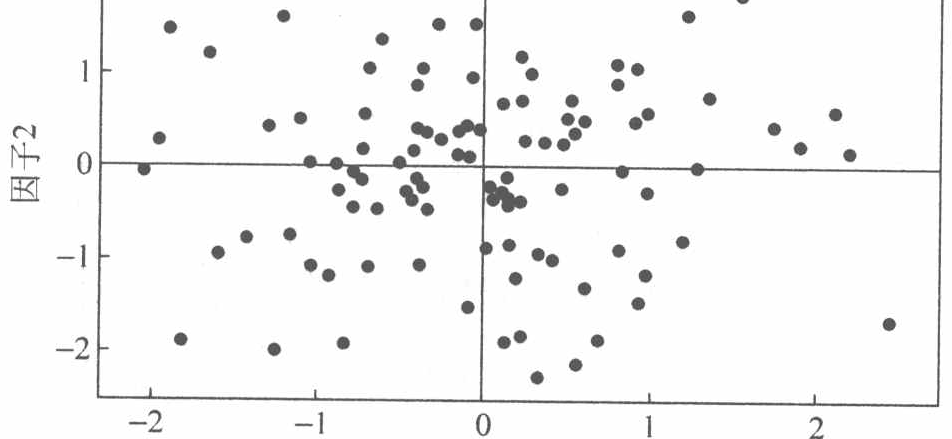
\includegraphics[width=80.6mm]{figs/fig_pg414_1.png}
\phantomsection\label{fig:9.4}\mvcap{图 9.4\quad 对股票价格数据用式(9-58)得到的因子 1 和 2 的因子得分\par（因子载荷的极大似然估计）}
\end{mvfigure}

%% ===== pg-415 =====

% ---- pg-415 （书页 403） ----

\mvbold{评注}\quad 可以很简单地构造具有好的直观性质的因子得分. 将在一个因子上有高载荷(例如绝对值大于 0.40)的变量归为一组. 可以通过把组内变量的(标准化)观测值根据载荷的符号求和得到因子得分. 通过这些简单的因子得分来代替标准化数据可以使数据简化. 简单因子得分与用最小二乘或回归方法得到的因子得分之间通常有高度相关性.

\noindent\textbf{例 9.13}\quad (由因子分析分组创建简单综合得分)

例 9.4 中股票价格数据主成分因子分析的载荷估计为
\[
\tilde{\mathbf{L}}=
\begin{bmatrix}
0.732&-0.437\\
0.831&-0.280\\
0.726&-0.374\\
0.605&0.694\\
0.563&0.719
\end{bmatrix}
\qquad\text{与}\qquad
\tilde{\mathbf{L}}^*=\tilde{\mathbf{L}}\mathbf{T}=
\begin{bmatrix}
0.852&0.030\\
0.851&0.214\\
0.813&0.079\\
0.133&0.911\\
0.084&0.909
\end{bmatrix}
\]
对每个因子, 把 $\tilde{\mathbf{L}}$ 中具有最大绝对值的载荷看成同等大小, 忽略小的载荷. 这样我们创建综合变量为线性组合
\[
\hat{f}_1=x_1+x_2+x_3+x_4+x_5
\]
\[
\hat{f}_2=x_4+x_5-x_1
\]
在实践中, 我们可以标准化这些新变量.

如果我们不是用 $\tilde{\mathbf{L}}$, 而是用方差最大旋转载荷矩阵 $\tilde{\mathbf{L}}^*$, 则简单因子得分为
\[
\hat{f}_1=x_1+x_2+x_3
\]
\[
\hat{f}_2=x_4+x_5
\]
确定高载荷和可忽略载荷是相当主观的判断. 最好选择与主题内容有关的线性组合. \hfill$\blacksquare$

虽然在因子分析中常常假定变量为多元正态的, 但是对大量的变量来说, 证明这个假定是很困难的. 像我们在第 4 章指出的那样, 边际变换可以帮助我们. 类似的, 因子得分可以是也可以不是正态分布的, 双变量因子得分散布图可以产生各种各样非椭圆形状的图形. 在运用因子得分作其他分析之前, 应对其图形作检查. 它们可以揭示出远离中心的值和(可能的)非正态性的程度.

\section{因子分析的展望和建议}
\phantomsection\label{sec:9.6}

在因子分析研究中, 必须作出许多决策. 大概最重要的决策是选择公共因子数 $m$. 虽然已知 $m$ 时对模型充分性有大样本检验, 但这只是对近似正态分布的数据适用. 而且, 若变量数和观测数都大, 检验将会很有把握地拒绝极小 $m$ 的模型, 而正是此时因子分析可提供一个有用的近似. 最为常见的是, $m$ 最后的选定基于下述考虑的综合: (1)所解释的样本方差的比例, (2)题材知识, 以及 (3)结论的“合理程度”.

解法和旋转类型的选择并非决定性的决策, 事实上, 大多数满意的因子分析都试用了不止一种旋转并且所有结果实质上确认同一因子结构.

在现阶段, 因子分析仍然是一种艺术, 并且尚没有一种单一的策略可以获得完美的成功. 我们建议和详细阐述一种合情合理的选择:

\noindent 1.\quad 执行主成分因子分析. 这个方法对第一次考察数据尤其合适(不要求 $\mathbf{R}$ 或 $\mathbf{S}$ 是非奇异的).

%% ===== pg-416 =====

% ---- pg-416 （书页 404） ----

(a) 画因子得分图, 找可疑观测值.
计算对各观测值的标准化得分和 4.6 节所述的平方距离.
(b) 试用最大方差旋转.
2. 执行包括最大方差旋转在内的极大似然因子分析.
3. 比较从两个因子分析得到的解.
(a) 载荷的分组方式是否相同?
(b) 画出从主成分得到的因子得分图, 对比从极大似然分析得到的图形.
4. 对其他的公共因子数 $m$, 重复前三个步骤. 有必要将额外的因子放入来理解和阐述该数据吗?
5. 对大数据集, 将它们分为两半并且对每一半都执行因子分析. 比较这两个结果, 并与从完整数据集所得结果做比较, 以检查解的稳定性. (数据剖分时可以把前一半放在一组中, 把后一半放在另一组中. 这能揭示随时间而发生的变化.)

\noindent\textbf{例 9.14}\quad (鸡的骨骼数据的因子分析)

我们介绍对白来亨鸡的骨骼和颅骨测量的几个因子分析的结果, 原始数据取自邓恩(Dunn, 见文献[5]). 邓恩数据的因子分析, 起初由赖特(Wright, 见文献[15])研究, 他从跟我们不同的相关矩阵着手分析.

全数据集由对鸡骨骼大小的 $n=276$ 个测量值(数据)组成:
\[
\begin{array}{r@{\ }l}
\text{头：} & \left\{\begin{array}{l}X_1=\text{颅骨长度}\\ X_2=\text{颅骨幅宽}\end{array}\right.\\[10pt]
\text{腿：} & \left\{\begin{array}{l}X_3=\text{股骨长}\\ X_4=\text{胫骨长}\end{array}\right.\\[10pt]
\text{翅：} & \left\{\begin{array}{l}X_5=\text{肱骨长}\\ X_6=\text{尺骨长}\end{array}\right.
\end{array}
\]

把样本相关矩阵
\[
\mathbf{R}=\begin{bmatrix}
1.000&0.505&0.569&0.602&0.621&0.603\\
0.505&1.000&0.422&0.467&0.482&0.450\\
0.569&0.422&1.000&0.926&0.877&0.878\\
0.602&0.467&0.926&1.000&0.874&0.894\\
0.621&0.482&0.877&0.874&1.000&0.937\\
0.603&0.450&0.878&0.894&0.937&1.000
\end{bmatrix}
\]

用主成分法和极大似然法对 $m=3$ 因子模型作因子分析. 结果显示于\hyperref[tab:9.10]{表 9.10}.\footnote{{\footnotesize 注意在极大似然解中胫骨长的估计特殊方差为 0.00. 这表明极大化似然函数可以产生海伍德情况. 重做我们的结果的读者若使用 SAS 或类似软件, 应该试一下 Hey(wood) 选择.}}

旋转之后, 求解的两种方法出现略为不同的结果. 将注意力集中于主成分法和被解释的样本总方差的累积比, 我们看到三因子解是有道理的. 第三个因子解释附加样本变差的一个“显著的”比例. 第一个因子表现为体格大小因子, 为翅和腿的大小所左右. 第二和第三因子, 总体上描绘颅骨大小, 可以分别给予与变量相同的名字, 即颅骨幅宽和颅骨长度.

%% ===== pg-417 =====

% ---- pg-417 （书页 405） ----

\begin{mvtable}
\phantomsection\label{tab:9.10}\mvtabcap{表 9.10\quad 鸡的骨骼数据的因子分析}
\mvsub{主成分法}
\small
\begin{tabular}{lccccccc}
\toprule
& \multicolumn{3}{c}{因子载荷估计} & \multicolumn{3}{c}{旋转因子载荷估计} & \\
\cmidrule(lr){2-4}\cmidrule(lr){5-7}
变\quad 量 & $F_1$ & $F_2$ & $F_3$ & $F_1^{*}$ & $F_2^{*}$ & $F_3^{*}$ & $\tilde{\psi}_i$\\
\midrule
1. 颅骨长度 & 0.741 & 0.350 & 0.573 & 0.355 & 0.244 & 0.902 & 0.00\\
2. 颅骨幅宽 & 0.604 & 0.720 & $-0.340$ & 0.235 & 0.949 & 0.211 & 0.00\\
3. 股骨长 & 0.929 & $-0.233$ & $-0.075$ & 0.921 & 0.164 & 0.218 & 0.08\\
4. 胫骨长 & 0.943 & $-0.175$ & $-0.067$ & 0.904 & 0.212 & 0.252 & 0.08\\
5. 肱骨长 & 0.948 & $-0.143$ & $-0.045$ & 0.888 & 0.228 & 0.283 & 0.08\\
6. 尺骨长 & 0.945 & $-0.189$ & $-0.047$ & 0.908 & 0.192 & 0.264 & 0.07\\
\midrule
\makecell[l]{所解释的(标准化)\\样本总方差的\\累积比例}
 & 0.743 & 0.873 & 0.950 & 0.576 & 0.763 & 0.950 & \\
\bottomrule
\end{tabular}

\vspace{10pt}
\mvsub{极大似然法}
\begin{tabular}{lccccccc}
\toprule
& \multicolumn{3}{c}{因子载荷估计} & \multicolumn{3}{c}{旋转因子载荷估计} & \\
\cmidrule(lr){2-4}\cmidrule(lr){5-7}
变\quad 量 & $F_1$ & $F_2$ & $F_3$ & $F_1^{*}$ & $F_2^{*}$ & $F_3^{*}$ & $\hat{\psi}_i$\\
\midrule
1. 颅骨长度 & 0.602 & 0.214 & 0.286 & 0.467 & 0.506 & 0.128 & 0.51\\
2. 颅骨幅宽 & 0.467 & 0.177 & 0.652 & 0.211 & 0.792 & 0.050 & 0.33\\
3. 股骨长 & 0.926 & 0.145 & $-0.057$ & 0.890 & 0.289 & 0.084 & 0.12\\
4. 胫骨长 & 1.000 & 0.000 & $-0.000$ & 0.936 & 0.345 & $-0.073$ & 0.00\\
5. 肱骨长 & 0.874 & 0.463 & $-0.012$ & 0.831 & 0.362 & 0.396 & 0.02\\
6. 尺骨长 & 0.894 & 0.336 & $-0.039$ & 0.857 & 0.325 & 0.272 & 0.09\\
\midrule
\makecell[l]{所解释的(标准化)\\样本总方差的\\累积比例}
 & 0.667 & 0.738 & 0.823 & 0.559 & 0.779 & 0.823 & \\
\bottomrule
\end{tabular}
\end{mvtable}

旋转极大似然因子载荷与用主成分法生成的因子载荷对第一因子是一致的, 但对第二和第三因子不一致. 对极大似然法, 第二因子是代表头部大小. 第三因子含义不清, 而且可能是不需要的.

对保留三个或更少因子的进一步支持, 由从极大似然估计得到的残差阵提供:
\[
\mathbf{R}-\hat{\mathbf{L}}_z\hat{\mathbf{L}}_z'-\hat{\boldsymbol{\Psi}}_z=
\left[\begin{array}{rrrrrr}
0.000& & & & & \\
-0.000&0.000& & & & \\
-0.003&0.001&0.000& & & \\
0.000&0.000&0.000&0.000& & \\
-0.001&0.000&0.000&0.000&0.000& \\
0.004&-0.001&-0.001&0.000&-0.000&0.000
\end{array}\right]
\]

该矩阵的全部元都很小. 我们将继续探索此例的 $m=3$ 因子模型. $m=2$ 因子模型在练习 9.10 中考虑.

从带有极大似然估计旋转的\hyperref[eq:9-58]{式(9-58)}产生的对因子 1 和因子 2 的因子得分, 示于\hyperref[fig:9.5]{图 9.5} 中. 该图可让我们确认那些出于某种原因与其余观测值不一致的观测值. 可能的离群值在图上已圈出.

%% ===== pg-418 =====

% ---- pg-418 （书页 406） ----

\begin{mvfigure}
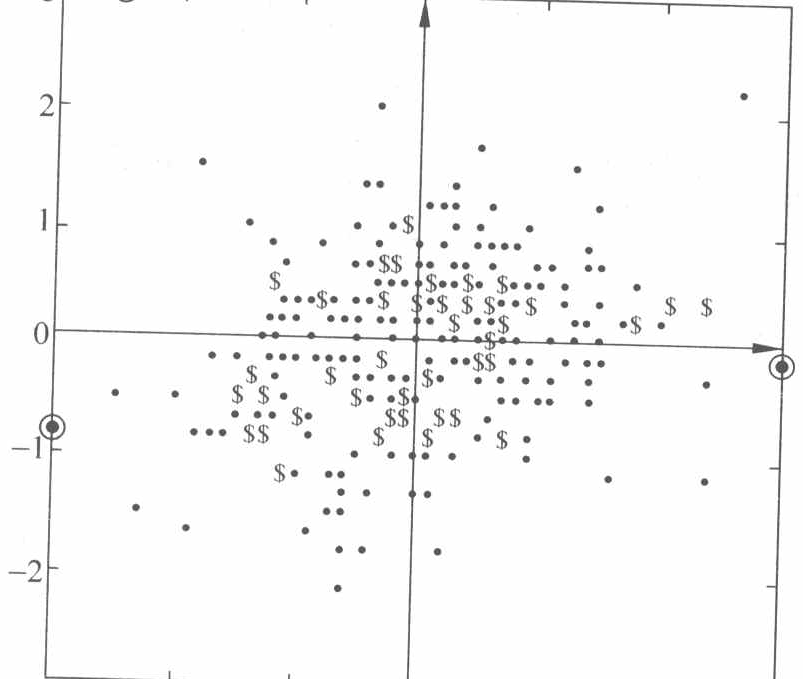
\includegraphics[width=68.0mm]{figs/fig_pg418_1.png}
\phantomsection\label{fig:9.5}\mvcap{图 9.5\quad 鸡的骨骼数据前两个因子的因子得分}
\end{mvfigure}

画出用主成分和极大似然估计因子载荷而得到因子得分配对的图形也是有意义的. 对于鸡的骨骼数据, 因子得分配对的图示于\hyperref[fig:9.6]{图 9.6}. 如果在某个因子上诸载荷一致, 则此得分配对将紧紧聚集在通过原点的 $45^\circ$ 直线附近. 不一致的那些载荷, 将产生偏离这一模式的因子得分. 如果后一情况出现, 它通常与最后面的因子有关, 并且可能表明因子数太大了, 即最后的那些因子没有多大意义. 这似乎正是鸡的骨骼数据中第三因子出现的情况, 如\hyperref[fig:9.6]{图 9.6} 的(c)图所示.

\begin{mvfigure}
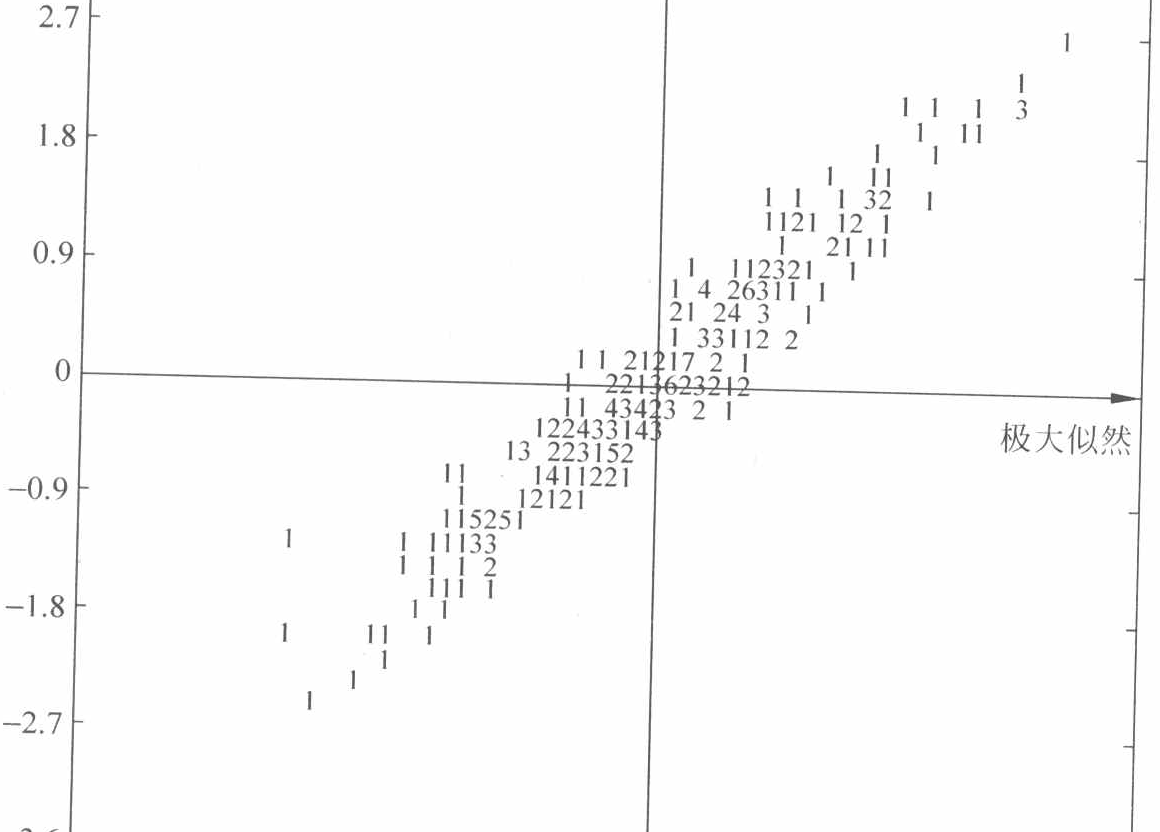
\includegraphics[width=98.2mm]{figs/fig_pg418_2.png}
\mvcap{(a) 第一因子}
\phantomsection\label{fig:9.6}\mvcap{图 9.6\quad 鸡的骨骼数据的因子得分配对\par（用主成分法和极大似然法估计载荷）}
\end{mvfigure}

%% ===== pg-419 =====

% ---- pg-419 （书页 407） ----

\begin{mvfigure}
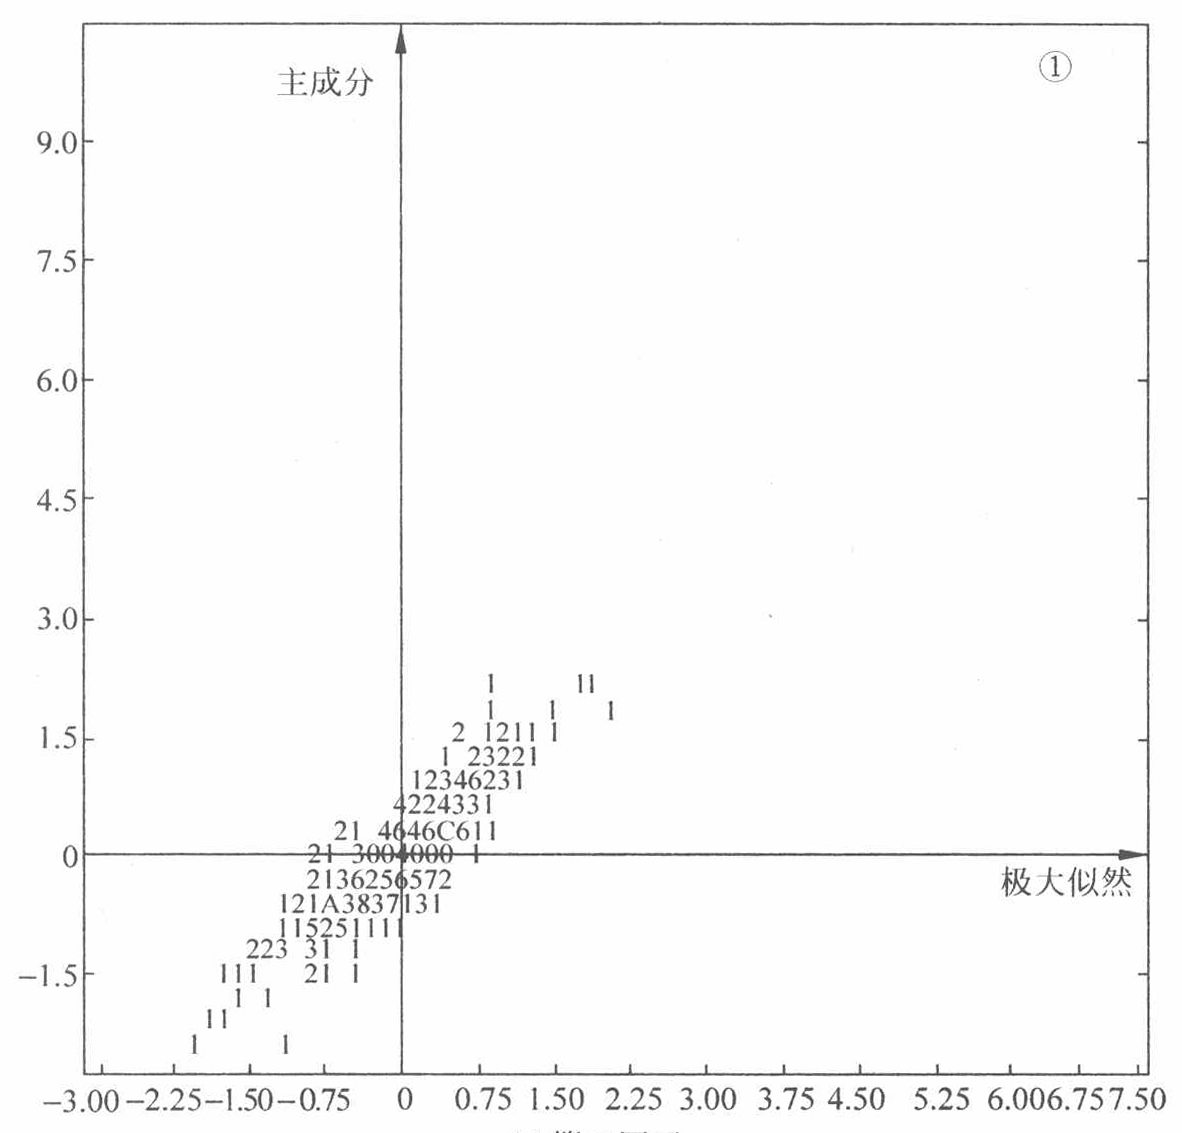
\includegraphics[width=100.2mm]{figs/fig_pg419_1.png}
\mvcap{(b) 第二因子}
\end{mvfigure}

\begin{mvfigure}
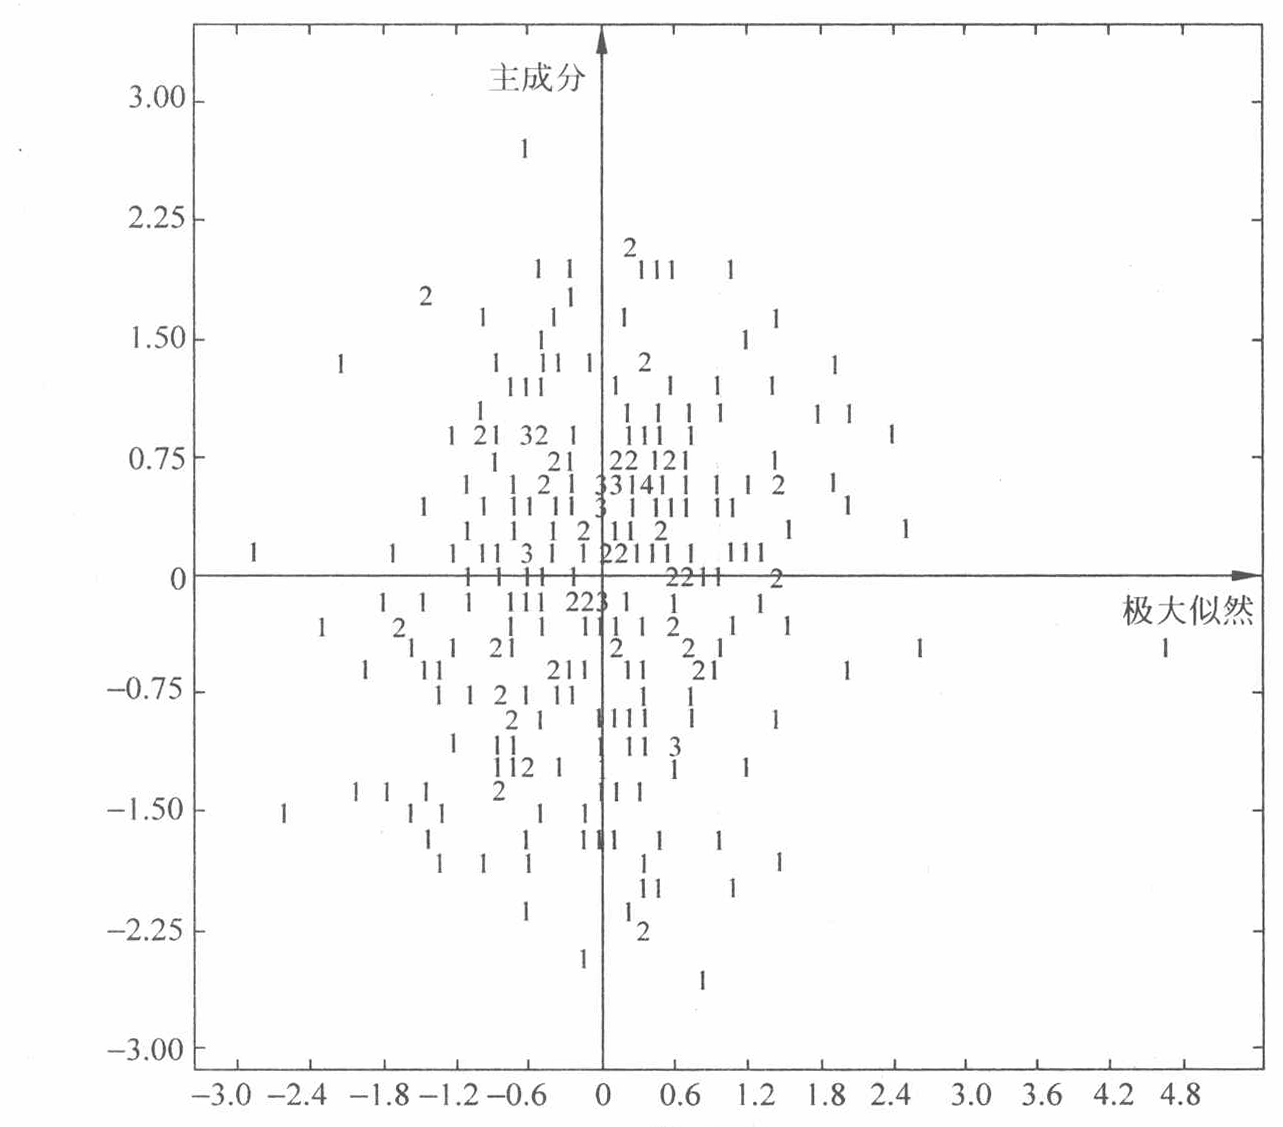
\includegraphics[width=108.6mm]{figs/fig_pg419_2.png}
\mvcap{(c) 第三因子}
\phantomsection\label{fig:9.6-2}\phantomsection\label{fig:9.6-2-2}\mvcap{图 9.6\quad （续）}
\end{mvfigure}

%% ===== pg-420 =====

% ---- pg-420 （书页 408） ----

利用从两种解法估计出的载荷得到的因子得分配对图, 也是探测离群值的好工具. 若对某因子的载荷趋向一致, 离群值将在 $45^\circ$ 直线的邻域中出现, 但却远离原点和其余点聚集处. 从\hyperref[fig:9.6]{图 9.6} 的(b)图可以清楚看到, 276 个观测值中只有一个点与其他点不一致. 它有一个少见的大 $F_2$ 得分. 要是除去此点 $[39.1, 39.3, 75.7, 115, 73.4, 69.1]$, 并重作分析, 载荷不会有明显改变.

在数据集大时, 应将它分为两个(大致)相等的组, 并且在每个组上完成因子分析. 这些分析的结果可以彼此作比较, 还可以与全部数据集的分析作比较, 以检查解的稳定性. 如果结果相互一致, 对解的信任程度就增强了.

鸡的骨骼数据曾被分为 $n_1=137$ 个和 $n_2=139$ 个观察值的两组. 得到的样本相关矩阵为
\[
\mathbf{R}_1=\left[\begin{array}{rrrrrr}
1.000& & & & & \\
0.696&1.000& & & & \\
0.588&0.540&1.000& & & \\
0.639&0.575&0.901&1.000& & \\
0.694&0.606&0.844&0.835&1.000& \\
0.660&0.584&0.866&0.863&0.931&1.000
\end{array}\right]
\]
及
\[
\mathbf{R}_2=\left[\begin{array}{rrrrrr}
1.000& & & & & \\
0.366&1.000& & & & \\
0.572&0.352&1.000& & & \\
0.587&0.406&0.950&1.000& & \\
0.587&0.420&0.909&0.911&1.000& \\
0.598&0.386&0.894&0.927&0.940&1.000
\end{array}\right]
\]

旋转后的估计载荷、特殊方差及对 $m=3$ 因子模型主成分分解所解释的(标准化)样本总方差的比例, 在\hyperref[tab:9.11]{表 9.11} 中给出.

\begin{mvtable}
\phantomsection\label{tab:9.11}\mvtabcap{表 9.11}
\small
\begin{tabular}{lcccc|cccc}
\toprule
& \multicolumn{4}{c}{第一组 旋转因子载荷估计} & \multicolumn{4}{c}{第二组 旋转因子载荷估计}\\
& \multicolumn{4}{c}{($n_1=137$ 个观测值)} & \multicolumn{4}{c}{($n_2=139$ 个观测值)}\\
\cmidrule(r){2-5}\cmidrule(l){6-9}
变\quad 量 & $F_1^{*}$ & $F_2^{*}$ & $F_3^{*}$ & $\tilde{\psi}_i$ & $F_1^{*}$ & $F_2^{*}$ & $F_3^{*}$ & $\hat{\psi}_i$\\
\midrule
1. 颅骨长度 & 0.360 & 0.361 & 0.853 & 0.01 & 0.352 & 0.921 & 0.167 & 0.00\\
2. 颅骨幅宽 & 0.303 & 0.899 & 0.312 & 0.00 & 0.203 & 0.145 & 0.968 & 0.00\\
3. 股骨长 & 0.914 & 0.238 & 0.175 & 0.08 & 0.930 & 0.239 & 0.130 & 0.06\\
4. 胫骨长 & 0.877 & 0.270 & 0.242 & 0.10 & 0.925 & 0.248 & 0.187 & 0.05\\
5. 肱骨长 & 0.830 & 0.247 & 0.395 & 0.11 & 0.912 & 0.252 & 0.208 & 0.06\\
6. 尺骨长 & 0.871 & 0.231 & 0.332 & 0.08 & 0.914 & 0.272 & 0.168 & 0.06\\
\midrule
\makecell[l]{所解释的(标准化)\\样本总方差的\\累积比例}
 & 0.546 & 0.743 & 0.940 & & 0.593 & 0.780 & 0.962 & \\
\bottomrule
\end{tabular}
\end{mvtable}

%% ===== pg-421 =====

% ---- pg-421 （书页 409） ----

对鸡的骨骼测量值的两组结果很类似. 因子 $F_2^{*}$ 和 $F_3^{*}$ 的颅骨长度和颅骨幅宽的标号互换, 但它们一起代表头部大小. 第一因子 $F_1^{*}$ 再次表现为是体格大小因子, 受腿和翅膀控制. 与对整个数据集的主成分分析给出的结果, 有着同样的阐述. 解是相当稳定的, 并且我们十分相信, 大载荷是“真实的”. 然而像我们已经指出过的, 三个因子可能是太多了. 一个单因子或双因子模型对鸡的骨骼数据已是十分充分的, 我们鼓励大家重作因子分析, 并采用更少因子和变换解法(见练习 9.10). \hfill$\blacksquare$

因子分析对行为科学和社会科学有着巨大的直观上的吸引力. 在这些领域很自然会认为, 对动物和人类过程的多变量观测值是潜在的、不能观测的“特性”的表现形式. 因子分析提供了一条途径, 用这些特性来解释行为观察变量.

在最后我们要说, 因子分析仍然是十分主观的. 我们的例子以及大多数出版资料中, 因子分析模型都用少数可阐述因子提供合理解释. 实际上, 绝大多数因子分析并没产生如此明确的结果. 不幸的是, 评价因子分析质量的法则尚未很好量化, 质量问题似乎只好依赖一个

\par\vspace{2pt}{\centering “哇”准则\par}\vspace{2pt}

如果在仔细检查因子分析的时候, 研究者能够喊出“哇, 我明白了这些因子”的时候, 就可看作是成功运用了因子分析.

\mvsub{补充 9A\quad 极大似然估计的某些计算细节}

虽然不能得到极大似然估计 $\hat{\mathbf{L}}$ 和 $\hat{\boldsymbol{\Psi}}$ 的简单解析表达式, 但可以证明它们满足某些方程. 以一个不知结构的协方差矩阵的极大似然估计量 $\mathbf{S}_n=(1/n)\sum\limits_{j=1}^{n}(\mathbf{X}_j-\bar{\mathbf{X}})(\mathbf{X}_j-\bar{\mathbf{X}})'$ 来表示这些条件方程, 是毫不奇怪的. 一些因子分析者采用通常的样本协方差 $\mathbf{S}$, 却仍用极大似然的名称来称呼得到的估计. 此项修改等同于采用从威沙特分布 $\sum\limits_{j=1}^{n}(\mathbf{X}_j-\bar{\mathbf{X}})\cdot(\mathbf{X}_j-\bar{\mathbf{X}})'$ 得到的似然估计, 而忽略由 $\bar{\mathbf{X}}$ 的正态密度作出的微小贡献. 既然 $\mathbf{S}_n$ 和 $\mathbf{S}$ 都产生同样的相关矩阵, $\mathbf{R}$ 的因子分析当然不受选用 $\mathbf{S}_n$ 还是选用 $\mathbf{S}$ 的影响.

\mvthm{结论 9A.1}{} \quad 令 $\mathbf{x}_1,\mathbf{x}_2,\cdots,\mathbf{x}_n$ 是来自正态总体的随机样本. 将\hyperref[eq:9-25]{式(9-25)}在唯一性条件(9-26)约束下取最大化, 得到极大似然估计 $\hat{\mathbf{L}}$ 和 $\hat{\boldsymbol{\Psi}}$. 它们满足
\phantomsection\label{eq:9A-1}
\begin{equation}
(\hat{\boldsymbol{\Psi}}^{-1/2}\mathbf{S}_n\hat{\boldsymbol{\Psi}}^{-1/2})(\hat{\boldsymbol{\Psi}}^{-1/2}\hat{\mathbf{L}})=(\hat{\boldsymbol{\Psi}}^{-1/2}\hat{\mathbf{L}})(\mathbf{I}+\hat{\boldsymbol{\Delta}}) \tag{9A-1}
\end{equation}
故 $\hat{\boldsymbol{\Psi}}^{-1/2}\hat{\mathbf{L}}$ 的第 $j$ 列是 $\hat{\boldsymbol{\Psi}}^{-1/2}\mathbf{S}_n\hat{\boldsymbol{\Psi}}^{-1/2}$ 的(非规范化)特征向量, 对应于特征值 $1+\hat{\Delta}_j$. 这里
\[
\mathbf{S}_n=n^{-1}\sum_{j=1}^{n}(\mathbf{x}_j-\bar{\mathbf{x}})(\mathbf{x}_j-\bar{\mathbf{x}})'=n^{-1}(n-1)\mathbf{S}\qquad\text{且}\qquad
\hat{\Delta}_1\geqslant\hat{\Delta}_2\geqslant\cdots\geqslant\hat{\Delta}_m
\]
还有, 在收敛处,
\phantomsection\label{eq:9A-2}
\begin{equation}
\hat{\psi}_i=\mathbf{S}_n-\hat{\mathbf{L}}\hat{\mathbf{L}}'\ \text{的第}\ i\ \text{个对角元} \tag{9A-2}
\end{equation}
和
\[
\mathrm{tr}(\hat{\boldsymbol{\Sigma}}^{-1}\mathbf{S}_n)=p
\]
我们不去考虑证明的细节, 但很明显, $\hat{\boldsymbol{\mu}}=\bar{\mathbf{x}}$, 考虑到对数似然函数, 会引向在 $\mathbf{L}$ 和 $\boldsymbol{\Psi}$ 上求 $-(n/2)[\ln|\boldsymbol{\Sigma}|+\mathrm{tr}(\boldsymbol{\Sigma}^{-1}\mathbf{S}_n)]$ 的最大化. 等价的, 由于 $\mathbf{S}_n$ 和 $p$ 在最大化中是常数, 我们把
\phantomsection\label{eq:9A-3}
\begin{equation}
h(\hat{\boldsymbol{\mu}},\boldsymbol{\Psi},\mathbf{L})=\ln|\boldsymbol{\Sigma}|-\ln|\mathbf{S}_n|+\mathrm{tr}(\boldsymbol{\Sigma}^{-1}\mathbf{S}_n)-p \tag{9A-3}
\end{equation}

%% ===== pg-422 =====

% ---- pg-422 （书页 410） ----

在 $\mathbf{L}'\boldsymbol{\Psi}^{-1}\mathbf{L}=\boldsymbol{\Delta}$ 为对角阵的约束下, 予以最小化. \hfill$\blacksquare$

\noindent\mvbold{评注}\quad 劳雷和马克斯韦尔(见文献[10]), 以及许多做因子分析的工作者, 用协方差的无偏估计 $\mathbf{S}$ 代替极大似然估计 $\mathbf{S}_n$. 现在, 对正态数据, $(n-1)\mathbf{S}$ 服从威沙特分布[见\hyperref[eq:4-21]{式(4-21)}和式(4-23)]. 如果我们略去包含 $(\boldsymbol{\mu}-\bar{\mathbf{x}})$ 的第二项对似然函数(9-25)的贡献, 则在 $\mathbf{L}$ 和 $\boldsymbol{\Psi}$ 上将缩减了的似然函数做最大化, 等价于在 $\mathbf{L}$ 和 $\boldsymbol{\Psi}$ 上将威沙特似然函数
\[
\text{似然函数}\propto|\boldsymbol{\Sigma}|^{-(n-1)/2}e^{-[(n-1)/2]\mathrm{tr}(\boldsymbol{\Sigma}^{-1}\mathbf{S})}
\]
最大化. 等价的, 我们可以把
\[
\ln|\boldsymbol{\Sigma}|+\mathrm{tr}(\boldsymbol{\Sigma}^{-1}\mathbf{S}_n)
\]
最小化, 或者像\hyperref[eq:9A-3]{式(9A-3)}那样把
\[
\ln|\boldsymbol{\Sigma}|+\mathrm{tr}(\boldsymbol{\Sigma}^{-1}\mathbf{S})-\ln|\mathbf{S}|-p
\]
最小化. 在这些条件下, 以 $\mathbf{S}$ 代替 $\mathbf{S}_n$, 结论 9A-1 成立. 还有, 对大 $n$, $\mathbf{S}$ 和 $\mathbf{S}_n$ 几乎是相等的, 并且相应的极大似然估计 $\hat{\mathbf{L}}$ 和 $\hat{\boldsymbol{\Psi}}$ 会类似. 为检验因子模型[见\hyperref[eq:9-39]{式(9-39)}], 若采用实际的似然函数(9-25), 应该把 $|\hat{\mathbf{L}}\hat{\mathbf{L}}'+\hat{\boldsymbol{\Psi}}|$ 与 $|\mathbf{S}_n|$ 作比较, 如用前述的威沙特似然函数去导出 $\hat{\mathbf{L}}$ 和 $\hat{\boldsymbol{\Psi}}$, 就应该把 $|\hat{\mathbf{L}}\hat{\mathbf{L}}'+\hat{\boldsymbol{\Psi}}|$ 与 $|\mathbf{S}|$ 作比较.

\mvsub{推荐的计算方案}

对 $m>1$, 条件 $\mathbf{L}'\boldsymbol{\Psi}^{-1}\mathbf{L}=\boldsymbol{\Delta}$ 有效地给 $\mathbf{L}$ 和 $\boldsymbol{\Psi}$ 的元素施加了 $m(m-1)/2$ 个限制, 并且在这些限制的约束下以一种迭代方式解出似然方程. 方法可如下:

1. 计算特殊方差 $\psi_1,\psi_2,\cdots,\psi_p$ 的初始估计. 朱瑞司柯克(见文献[8])建议设
\phantomsection\label{eq:9A-4}
\begin{equation}
\hat{\psi}_i=\left(1-\frac{1}{2}\cdot\frac{m}{p}\right)\left(\frac{1}{s^{ii}}\right) \tag{9A-4}
\end{equation}
其中 $s^{ii}$ 是 $\mathbf{S}^{-1}$ 的第 $i$ 个对角元.

2. 已知 $\hat{\boldsymbol{\Psi}}$, 计算“再调节了唯一性的”协方差矩阵
\phantomsection\label{eq:9A-5}
\begin{equation}
\mathbf{S}^{*}=\hat{\boldsymbol{\Psi}}^{-1/2}\mathbf{S}_n\hat{\boldsymbol{\Psi}}^{-1/2} \tag{9A-5}
\end{equation}
的前 $m$ 个不同特征值 $\hat{\lambda}_1>\hat{\lambda}_2>\cdots>\hat{\lambda}_m>1$, 以及对应的特征向量 $\hat{\mathbf{e}}_1,\hat{\mathbf{e}}_2,\cdots,\hat{\mathbf{e}}_m$. 令 $\tilde{\mathbf{E}}=[\hat{\mathbf{e}}_1\ \vdots\ \hat{\mathbf{e}}_2\ \vdots\ \cdots\ \vdots\ \hat{\mathbf{e}}_m]$ 是规范化特征向量的 $p\times m$ 矩阵, $\tilde{\boldsymbol{\Lambda}}=$ 对角阵$[\hat{\lambda}_1,\hat{\lambda}_2,\cdots,\hat{\lambda}_m]$ 是特征值的 $m\times m$ 对角阵. 从\hyperref[eq:9A-1]{式(9A-1)}, $\tilde{\boldsymbol{\Lambda}}=\mathbf{I}+\hat{\boldsymbol{\Delta}}$, $\tilde{\mathbf{E}}=\hat{\boldsymbol{\Psi}}^{-1/2}\hat{\mathbf{L}}\hat{\boldsymbol{\Delta}}^{-1/2}$. 这样, 我们得到估计
\phantomsection\label{eq:9A-6}
\begin{equation}
\hat{\mathbf{L}}=\hat{\boldsymbol{\Psi}}^{1/2}\tilde{\mathbf{E}}\hat{\boldsymbol{\Delta}}^{1/2}=\hat{\boldsymbol{\Psi}}^{1/2}\tilde{\mathbf{E}}(\tilde{\boldsymbol{\Lambda}}-\mathbf{I})^{1/2} \tag{9A-6}
\end{equation}

3. 将\hyperref[eq:9A-6]{式(9A-6)}得到的 $\hat{\mathbf{L}}$ 代进似然函数(9A-3), 并就 $\hat{\psi}_1,\hat{\psi}_2,\cdots,\hat{\psi}_p$ 将结果最小化. 必须用到一个数值搜索程序. 在步骤 2 用从最小化得到的值 $\hat{\psi}_1,\hat{\psi}_2,\cdots,\hat{\psi}_p$ 去生成一个新的 $\hat{\mathbf{L}}$. 重复步骤 2 和 3 直到收敛为止, 即直到 $\hat{l}_{ij}$ 和 $\hat{\psi}_i$ 的相继值之差可以忽略为止.

\noindent\mvbold{评注}\quad 常常会发生这种情况: \hyperref[eq:9A-3]{式(9A-3)}中的目标函数对应于某个 $\hat{\psi}_i$ 的负值有相对的最小值. 这个解很清楚是不能接受的, 并说它是不真实的或是一个海伍德情况. 对大部分计算机程序包, 如在某个迭代中出现这种情况, 在下一步处理之前, 把负的 $\hat{\psi}_i$ 将改为小正数.

\mvsub{$\boldsymbol{\rho}=\mathbf{L}_z\mathbf{L}_z'+\boldsymbol{\Psi}_z$ 的极大似然估计}

当 $\boldsymbol{\Sigma}$ 有因子分析结构 $\boldsymbol{\Sigma}=\mathbf{L}\mathbf{L}'+\boldsymbol{\Psi}$, 则 $\boldsymbol{\rho}$ 可因子化, 为 $\boldsymbol{\rho}=\mathbf{V}^{-1/2}\boldsymbol{\Sigma}\mathbf{V}^{-1/2}=(\mathbf{V}^{-1/2}\mathbf{L})(\mathbf{V}^{-1/2}\mathbf{L})'+$

%% ===== pg-423 =====

% ---- pg-423 （书页 411） ----

$\mathbf{V}^{-1/2}\boldsymbol{\Psi}\mathbf{V}^{-1/2}=\mathbf{L}_z\mathbf{L}_z'+\boldsymbol{\Psi}_z$. 对标准化变量的载荷矩阵是 $\mathbf{L}_z=\mathbf{V}^{-1/2}\mathbf{L}$, 而相应的特殊方差矩阵是 $\boldsymbol{\Psi}_z=\mathbf{V}^{-1/2}\boldsymbol{\Psi}\mathbf{V}^{-1/2}$, 其中 $\mathbf{V}^{-1/2}$ 是对角阵, 其第 $i$ 个对角元为 $\sigma_{ii}^{-1/2}$. 若用 $\mathbf{R}$ 替代目标函数(9A-3)中的 $\mathbf{S}_n$, 研究者将
\phantomsection\label{eq:9A-7}
\begin{equation}
\ln\left(\frac{|\mathbf{L}_z\mathbf{L}_z'+\boldsymbol{\Psi}_z|}{|\mathbf{R}|}\right)+\mathrm{tr}[(\mathbf{L}_z\mathbf{L}_z'+\boldsymbol{\Psi}_z)^{-1}\mathbf{R}]-p \tag{9A-7}
\end{equation}
最小化.

引进对角阵 $\hat{\mathbf{V}}^{1/2}$, 它的第 $i$ 个对角元是 $\mathbf{S}_n$ 第 $i$ 个对角元的平方根, 我们可将目标函数(9A-7)写为
\phantomsection\label{eq:9A-8}
\begin{equation}
\begin{aligned}
&\ln\left(\frac{|\hat{\mathbf{V}}^{1/2}|}{|\hat{\mathbf{V}}^{1/2}|}\cdot\frac{|\mathbf{L}_z\mathbf{L}_z'+\boldsymbol{\Psi}_z|}{|\mathbf{R}|}\cdot\frac{|\hat{\mathbf{V}}^{1/2}|}{|\hat{\mathbf{V}}^{1/2}|}\right)\\
&\quad+\mathrm{tr}[(\mathbf{L}_z\mathbf{L}_z'+\boldsymbol{\Psi}_z)^{-1}\hat{\mathbf{V}}^{-1/2}\hat{\mathbf{V}}^{1/2}\mathbf{R}\hat{\mathbf{V}}^{1/2}\hat{\mathbf{V}}^{-1/2}]-p\\
&=\ln\left(\frac{|(\hat{\mathbf{V}}^{1/2}\mathbf{L}_z)(\hat{\mathbf{V}}^{1/2}\mathbf{L}_z)'+\hat{\mathbf{V}}^{1/2}\boldsymbol{\Psi}_z\hat{\mathbf{V}}^{1/2}|}{|\mathbf{S}_n|}\right)\\
&\quad+\mathrm{tr}[((\hat{\mathbf{V}}^{1/2}\mathbf{L}_z)(\hat{\mathbf{V}}^{1/2}\mathbf{L}_z)'+\hat{\mathbf{V}}^{1/2}\boldsymbol{\Psi}_z\hat{\mathbf{V}}^{1/2})^{-1}\mathbf{S}_n]-p\\
&\geqslant\ln\left(\frac{|\hat{\mathbf{L}}\hat{\mathbf{L}}'+\hat{\boldsymbol{\Psi}}|}{|\mathbf{S}_n|}\right)+\mathrm{tr}[(\hat{\mathbf{L}}\hat{\mathbf{L}}'+\hat{\boldsymbol{\Psi}})^{-1}\mathbf{S}_n]-p
\end{aligned} \tag{9A-8}
\end{equation}

最后一个不等号是因为极大似然估计 $\hat{\mathbf{L}}$ 和 $\hat{\boldsymbol{\Psi}}$ 使目标函数(9A-3)最小化. [对 $\mathbf{L}_z=\hat{\mathbf{V}}^{-1/2}\hat{\mathbf{L}}$ 和 $\boldsymbol{\Psi}_z=\hat{\mathbf{V}}^{-1/2}\hat{\boldsymbol{\Psi}}\hat{\mathbf{V}}^{-1/2}$, \hyperref[eq:9A-8]{式(9A-8)}中等号成立.] 因此, 在 $\mathbf{L}_z$ 和 $\boldsymbol{\Psi}_z$ 上将\hyperref[eq:9A-7]{式(9A-7)}最小化, 等价于从 $\mathbf{S}_n$ 得到 $\hat{\mathbf{L}}$ 和 $\hat{\boldsymbol{\Psi}}$ 并且用 $\hat{\mathbf{L}}_z=\hat{\mathbf{V}}^{-1/2}\hat{\mathbf{L}}$ 估计 $\mathbf{L}_z=\mathbf{V}^{-1/2}\mathbf{L}$ 和用 $\hat{\boldsymbol{\Psi}}_z=\hat{\mathbf{V}}^{-1/2}\hat{\boldsymbol{\Psi}}\hat{\mathbf{V}}^{-1/2}$ 估计 $\boldsymbol{\Psi}_z=\mathbf{V}^{-1/2}\boldsymbol{\Psi}\mathbf{V}^{-1/2}$. 后一估计过程的根据是极大似然估计的不变性[见\hyperref[eq:4-20]{式(4-20)}].

\mvsub{练习}

\noindent 9.1\quad 证明对 $p=3$ 个标准化随机变量 $Z_1$, $Z_2$ 和 $Z_3$ 的协方差矩阵
\[
\boldsymbol{\rho}=\begin{bmatrix}1.0&0.63&0.45\\0.63&1.0&0.35\\0.45&0.35&1.0\end{bmatrix}
\]
可以由 $m=1$ 的因子模型
\[
\left\{\begin{array}{l}
Z_1=0.9F_1+\epsilon_1\\
Z_2=0.7F_1+\epsilon_2\\
Z_3=0.5F_1+\epsilon_3
\end{array}\right.
\]
来生成, 其中 $\mathrm{Var}(F_1)=1$, $\mathrm{Cov}(\boldsymbol{\epsilon},F_1)=\mathbf{0}$, 且
\[
\boldsymbol{\Psi}=\mathrm{Cov}(\boldsymbol{\epsilon})=\begin{bmatrix}0.19&0&0\\0&0.51&0\\0&0&0.75\end{bmatrix}
\]
也即, 将 $\boldsymbol{\rho}$ 写成形式 $\boldsymbol{\rho}=\mathbf{L}\mathbf{L}'+\boldsymbol{\Psi}$.

\noindent 9.2\quad 利用练习 9.1 中的信息

(a) 计算共性方差 $h_i^2$, $i=1,2,3$, 并解释这些量.

%% ===== pg-424 =====

% ---- pg-424 （书页 412） ----

(b) 计算 $\mathrm{Corr}(Z_i,F_1)$, $i=1,2,3$. 哪个变量会在公共因子的“命名”上有最大的权重? 为什么?

\noindent 9.3\quad 练习 9.1 中的相关系数矩阵 $\boldsymbol{\rho}$ 的特征值和特征向量为
\[
\begin{aligned}
\lambda_1&=1.96, & \mathbf{e}_1'&=[0.625,0.593,0.507]\\
\lambda_2&=0.68, & \mathbf{e}_2'&=[-0.219,-0.491,0.843]\\
\lambda_3&=0.36, & \mathbf{e}_3'&=[0.749,-0.638,-0.177]
\end{aligned}
\]

(a) 假设 $m=1$ 的因子模型, 利用主成分解法计算载荷矩阵 $\mathbf{L}$ 及特别方差矩阵 $\boldsymbol{\Psi}$. 同练习 9.1 的结果作比较.
(b) 用第一公共因子解释的总体总方差的比例是多少?

\noindent 9.4\quad 已知练习 9.1 中的 $\boldsymbol{\rho}$ 和 $\boldsymbol{\Psi}$ 及 $m=1$ 的因子模型, 计算缩减相关系数矩阵 $\tilde{\boldsymbol{\rho}}=\boldsymbol{\rho}-\boldsymbol{\Psi}$ 及载荷矩阵 $\mathbf{L}$ 的主因子解. 这些结果是否与练习 9.1 相一致? 应该一致吗?

\noindent 9.5\quad 证明不等\hyperref[eq:9-19]{式(9-19)}
提示: 因为 $\mathbf{S}-\tilde{\mathbf{L}}\tilde{\mathbf{L}}'-\tilde{\boldsymbol{\Psi}}$ 在对角线上为 $\mathbf{0}$,
\[
(\mathbf{S}-\tilde{\mathbf{L}}\tilde{\mathbf{L}}'-\tilde{\boldsymbol{\Psi}}\ \text{元素的平方和})\leqslant(\mathbf{S}-\tilde{\mathbf{L}}\tilde{\mathbf{L}}'\ \text{元素的平方和})
\]
现在, $\mathbf{S}-\tilde{\mathbf{L}}\tilde{\mathbf{L}}'=\hat{\lambda}_{m+1}\hat{\mathbf{e}}_{m+1}\hat{\mathbf{e}}_{m+1}'+\cdots+\hat{\lambda}_p\hat{\mathbf{e}}_p\hat{\mathbf{e}}_p'=\hat{\mathbf{P}}_{(2)}\hat{\boldsymbol{\Lambda}}_{(2)}\hat{\mathbf{P}}_{(2)}'$, 其中 $\hat{\mathbf{P}}_{(2)}=[\hat{\mathbf{e}}_{m+1}\ \vdots\ \cdots\ \vdots\ \hat{\mathbf{e}}_p]$ 且 $\hat{\boldsymbol{\Lambda}}_{(2)}$ 是对角元为 $\hat{\lambda}_{m+1},\cdots,\hat{\lambda}_p$ 的对角阵.

利用($\mathbf{A}$ 元素的平方和) $=\mathrm{tr}\mathbf{A}\mathbf{A}'$ 及 $\mathrm{tr}[\hat{\mathbf{P}}_{(2)}\hat{\boldsymbol{\Lambda}}_{(2)}\hat{\boldsymbol{\Lambda}}_{(2)}\hat{\mathbf{P}}_{(2)}']=\mathrm{tr}[\hat{\boldsymbol{\Lambda}}_{(2)}\hat{\boldsymbol{\Lambda}}_{(2)}]$.

\noindent 9.6\quad 验证下列矩阵性质

(a) $(\mathbf{I}+\mathbf{L}'\boldsymbol{\Psi}^{-1}\mathbf{L})^{-1}\mathbf{L}'\boldsymbol{\Psi}^{-1}\mathbf{L}=\mathbf{I}-(\mathbf{I}+\mathbf{L}'\boldsymbol{\Psi}^{-1}\mathbf{L})^{-1}$
提示: 两边左乘 $(\mathbf{I}+\mathbf{L}'\boldsymbol{\Psi}^{-1}\mathbf{L})$.

(b) $(\mathbf{L}\mathbf{L}'+\boldsymbol{\Psi})^{-1}=\boldsymbol{\Psi}^{-1}-\boldsymbol{\Psi}^{-1}\mathbf{L}(\mathbf{I}+\mathbf{L}'\boldsymbol{\Psi}^{-1}\mathbf{L})^{-1}\mathbf{L}'\boldsymbol{\Psi}^{-1}$
提示: 两边右乘 $(\mathbf{L}\mathbf{L}'+\boldsymbol{\Psi})$ 并利用(a).

(c) $\mathbf{L}'(\mathbf{L}\mathbf{L}'+\boldsymbol{\Psi})^{-1}=(\mathbf{I}+\mathbf{L}'\boldsymbol{\Psi}^{-1}\mathbf{L})^{-1}\mathbf{L}'\boldsymbol{\Psi}^{-1}$
提示: 将(b)两边右乘 $\mathbf{L}$, 利用(a), 并将两边取转置, 注意 $(\mathbf{L}\mathbf{L}'+\boldsymbol{\Psi})^{-1}$, $\boldsymbol{\Psi}^{-1}$ 及 $(\mathbf{I}+\mathbf{L}'\boldsymbol{\Psi}^{-1}\mathbf{L})^{-1}$ 为对称矩阵.

\noindent 9.7\quad (因子模型参数化不必是唯一的.) 令因子模型 $p=2$ 和 $m=1$ 成立. 证明
\[
\sigma_{11}=l_{11}^2+\psi_1,\qquad \sigma_{12}=\sigma_{21}=l_{11}l_{21}
\]
\[
\sigma_{22}=l_{21}^2+\psi_2
\]
以及对给定 $\sigma_{11},\sigma_{22}$ 和 $\sigma_{12}$, 对 $\mathbf{L}$ 和 $\boldsymbol{\Psi}$ 存在无限多的选择.

\noindent 9.8\quad (唯一但不真实的解: 海伍德情形.)

对协方差矩阵为
\[
\boldsymbol{\Sigma}=\begin{bmatrix}1&0.4&0.9\\0.4&1&0.7\\0.9&0.7&1\end{bmatrix}
\]
的总体, 考虑 $m=1$ 的因子模型, 证明对满足 $\boldsymbol{\Sigma}=\mathbf{L}\mathbf{L}'+\boldsymbol{\Psi}$ 的 $\mathbf{L}$ 和 $\boldsymbol{\Psi}$ 有唯一的选择, 但 $\psi_3<0$, 因此这种选择是不可接受的.

%% ===== pg-425 =====

% ---- pg-425 （书页 413） ----

\noindent 9.9\quad 在法国的一项酒类调查中, 斯托塞尔(Stoetzel, 见文献[14])收集了 $n=1\ 442$ 个人对 $p=9$ 种酒的偏好, 并进行排名. 对排名顺序的 $9\times9$ 样本相关系数矩阵作的因子分析给出如下的载荷估计:

\begin{mvtable}
\small
\begin{tabular}{lccc}
\toprule
变量$(X_i)$ & \multicolumn{3}{c}{因子载荷估计}\\
\cmidrule(lr){2-4}
& $F_1$ & $F_2$ & $F_3$\\
\midrule
(蒸馏)酒 & 0.64 & 0.02 & 0.16\\
Kirsch 酒 & 0.50 & $-0.06$ & $-0.10$\\
Mirabelle 酒 & 0.46 & $-0.24$ & $-0.19$\\
朗姆酒 & 0.17 & 0.74 & $0.97^{*}$\\
白兰地 & $-0.29$ & 0.66 & $-0.39$\\
威士忌 & $-0.29$ & $-0.08$ & 0.09\\
Calvados 酒 & $-0.49$ & 0.20 & $-0.04$\\
科涅克白兰地 & $-0.52$ & $-0.03$ & 0.42\\
Armagnac 酒 & $-0.60$ & $-0.17$ & 0.14\\
\bottomrule
\end{tabular}
\end{mvtable}

\noindent{\footnotesize * 这个数据太大. 斯托塞尔采用了估计因子载荷的近似法, 结果, 它超过了最大值 0.64.}

已知这些结果, 斯托塞尔结论如下: 在法国关于酒的偏好最主要的原则是甜酒和烈酒之间的区别. 第二个激励因素是价格, 记住酒既昂贵又是种摆阔性的消费品, 就可理解这一点. 除了两种最大众化和最便宜的酒(朗姆酒和白兰地), 在产生对酒的喜好的判断上, 这第二个因子起的作用小得多, 第三个因子涉及社会性和地区性的判断差异(见文献[14]).

(a) 就你对所涉及的各种酒的知识来判断, 斯托塞尔的解释合理吗?

(b) 作图表示前两个因子的载荷对. 用图解法表示因子轴的正交旋转. 产生近似旋转载荷. 解释前两个因子的旋转载荷. 你的解释与斯托塞尔从未旋转载荷得到的因子解释一致吗? 请说明.

\noindent 9.10\quad 对鸡的骨骼测量值(见例 9.14)的相关系数矩阵为
\[
\left[\begin{array}{rrrrrr}
1.000& & & & & \\
0.505&1.000& & & & \\
0.569&0.422&1.000& & & \\
0.602&0.467&0.926&1.000& & \\
0.621&0.482&0.877&0.874&1.000& \\
0.603&0.450&0.878&0.894&0.937&1.000
\end{array}\right]
\]
以下因子载荷估计是由极大似然法求出的:

\begin{mvtable}
\small
\begin{tabular}{lcc|cc}
\toprule
& \multicolumn{2}{c}{因子载荷估计} & \multicolumn{2}{c}{因子载荷的最大方差旋转估计}\\
\cmidrule(r){2-3}\cmidrule(l){4-5}
变\quad 量 & $F_2^{*}$ & $F_1$ & $F_2$ & $F_1^{*}$\\
\midrule
1. 颅骨长度 & 0.602 & 0.200 & 0.484 & 0.411\\
2. 颅骨幅宽 & 0.467 & 0.154 & 0.375 & 0.319\\
3. 股骨长 & 0.926 & 0.143 & 0.603 & 0.717\\
4. 胫骨长 & 1.000 & 0.000 & 0.519 & 0.855\\
5. 肱骨长 & 0.874 & 0.476 & 0.861 & 0.499\\
6. 尺骨长 & 0.894 & 0.327 & 0.744 & 0.594\\
\bottomrule
\end{tabular}
\end{mvtable}

%% ===== pg-426 =====

% ---- pg-426 （书页 414） ----

用未旋转的因子载荷估计, 得出下列各项的极大似然估计.
(a) 特殊方差.
(b) 共性方差.
(c) 用各个因子解释的方差的比例.
(d) 残差矩阵 $\mathbf{R}-\hat{\mathbf{L}}_z\hat{\mathbf{L}}_z'-\hat{\boldsymbol{\Psi}}_z$.

\noindent 9.11\quad 参见练习 9.10 用未旋转和旋转的因子载荷估计, 计算最大方差准则的值. 对结果进行评论.

\noindent 9.12\quad 海龟测量值(见例 8.4)的对数的协方差矩阵为
\[
\mathbf{S}=10^{-3}\begin{bmatrix}11.072& & \\ 8.019&6.417& \\ 8.160&6.005&6.773\end{bmatrix}
\]
对一个 $m=1$ 的模型所作的极大似然因子载荷估计如下:

\begin{mvtable}
\small
\begin{tabular}{l|c}
\toprule
变\quad 量 & 因子载荷估计 $F_1$\\
\midrule
1. $\ln$(长度) & 0.102\ 2\\
2. $\ln$(宽度) & 0.075\ 2\\
3. $\ln$(高度) & 0.076\ 5\\
\bottomrule
\end{tabular}
\end{mvtable}

利用因子载荷估计, 得出以下各项的极大似然估计.
(a) 特殊方差.
(b) 共性方差.
(c) 可用因子解释的方差的比例.
(d) 残差矩阵 $\mathbf{S}_n-\hat{\mathbf{L}}\hat{\mathbf{L}}'-\hat{\boldsymbol{\Psi}}$.
提示: 用 $\mathbf{S}_n$ 换 $\mathbf{S}$.

\noindent 9.13\quad 参见练习 9.12. 计算\hyperref[eq:9-39]{式(9-39)}中的检验统计量. 有 $H_0:\boldsymbol{\Sigma}=\mathbf{L}\mathbf{L}'+\boldsymbol{\Psi}$ (取 $m=1$), $H_1:\boldsymbol{\Sigma}$ 无约束. 指出对此假设的检验, 在此例中为什么不能实现[见\hyperref[eq:9-40]{式(9-40)}].

\noindent 9.14\quad 极大似然因子载荷估计在\hyperref[eq:9A-6]{式(9A-6)}中由
\[
\hat{\mathbf{L}}=\hat{\boldsymbol{\Psi}}^{1/2}\tilde{\mathbf{E}}\hat{\boldsymbol{\Delta}}^{1/2}
\]
给出. 对此选择验证
\[
\hat{\mathbf{L}}\hat{\boldsymbol{\Psi}}^{-1}\hat{\mathbf{L}}=\hat{\boldsymbol{\Delta}}
\]
其中 $\hat{\boldsymbol{\Delta}}=\tilde{\boldsymbol{\Lambda}}-\mathbf{I}$ 是对角阵.

\noindent 9.15\quad 赫希切(Hirschley)和威克恩(Wichern)[7]调查对利润的会计测量和市场价值测量间的一致性、决定因素和用途. 他们研究的一部分是进行利润会计测量和经济利润市场估计的因子分析. 1977 年样本公司的会计历史、会计重置及市场价值测量的相关系数矩阵如下:

%% ===== pg-427 =====

% ---- pg-427 （书页 415） ----

\[
\begin{array}{l}
\textbf{变\quad 量}\\[4pt]
\text{资产历史收益率,HRA}\\
\text{股本历史收益率,HRE}\\
\text{销售历史收益率,HRS}\\
\text{资产重置收益率,RRA}\\
\text{股本重置收益率,RRE}\\
\text{销售重置收益率,RRS}\\
\text{市场 Q 比率,Q}\\
\text{市场相对溢价,REV}
\end{array}
\qquad
\left[\begin{array}{rrrrrrrr}
\text{HRA}&\text{HRE}&\text{HRS}&\text{RRA}&\text{RRE}&\text{RRS}&\text{Q}&\text{REV}\\
1.000& & & & & & & \\
0.738&1.000& & & & & & \\
0.731&0.520&1.000& & & & & \\
0.828&0.688&0.652&1.000& & & & \\
0.681&0.831&0.513&0.887&1.000& & & \\
0.712&0.543&0.826&0.867&0.692&1.000& & \\
0.625&0.322&0.579&0.639&0.419&0.608&1.000& \\
0.604&0.303&0.617&0.563&0.352&0.610&0.937&1.000
\end{array}\right]
\]

得到对 $m=3$ 因子模型因子载荷的旋转主成分估计如下:

\begin{mvtable}
\small
\begin{tabular}{l|ccc}
\toprule
变\quad 量 & \multicolumn{3}{c}{因子载荷估计}\\
\cmidrule(l){2-4}
& $F_1$ & $F_2$ & $F_3$\\
\midrule
HRA & 0.433 & 0.612 & 0.499\\
HRE & 0.125 & 0.892 & 0.234\\
HRS & 0.296 & 0.238 & 0.887\\
RRA & 0.406 & 0.708 & 0.483\\
RRE & 0.198 & 0.895 & 0.283\\
RRS & 0.331 & 0.414 & 0.789\\
Q & 0.928 & 0.160 & 0.294\\
REV & 0.910 & 0.079 & 0.355\\
\midrule
解释全部方差的累积比例 & 0.287 & 0.628 & 0.908\\
\bottomrule
\end{tabular}
\end{mvtable}

(a) 利用因子载荷估计, 确定特殊方差和共性方差.

(b) 确定残差矩阵 $\mathbf{R}-\hat{\mathbf{L}}_z\hat{\mathbf{L}}_z'-\hat{\boldsymbol{\Psi}}_z$. 已知此信息和上面表格中的解释总方差的累积比例, $m=3$ 的因子模型对这些数据是否恰当?

(c) 假设小于 0.4 的载荷估计是小的, 解释这三个因子. 例如, 会出现这种情况吗: 市场价值测量值表明的利润与会计测量值表明的利润不同? 你能将会计历史利润的测量值从会计重置测量中分出来吗?

\noindent 9.16\quad 证明由\hyperref[eq:9-50]{式(9-50)}构造的因子得分有样本均值向量 $\mathbf{0}$ 和零样本协方差.

\noindent 9.17\quad 参考例 9.12, 利用该例中的信息评估 $(\hat{\mathbf{L}}_z'\hat{\boldsymbol{\Psi}}_z^{-1}\hat{\mathbf{L}}_z)^{-1}$. 注意: 令 $\hat{\boldsymbol{\Psi}}_z$ 的第四对角元素为 0.01, 这样可以确定 $\hat{\boldsymbol{\Psi}}_z^{-1}$. 对标准化股价观测构造因子得分的回归和广义最小二乘法将得出几乎相同的结果吗? 提示: 参见\hyperref[eq:9-57]{式(9-57)}和随后的讨论.

\mvsub{以下练习需使用计算机.}

\noindent 9.18\quad 参见练习 8.16 的捕鱼数据
(a) 仅用测量值 $x_1-x_4$, 求出 $m=1$ 和 $m=2$ 的因子模型的主成分解.
(b) 仅用测量值 $x_1-x_4$, 求出 $m=1$ 和 $m=2$ 的因子模型的极大似然解.
(c) 旋转(a)和(b)的解. 比较这些解, 并加以评论. 解释每一个因子.
(d) 用测量值 $x_1-x_6$ 执行因子分析, 求因子的合理个数 $m$, 并比较旋转之后的主成分和

%% ===== pg-428 =====

% ---- pg-428 （书页 416） ----

极大似然解. 解释这些因子.

\noindent 9.19\quad 一家公司正试图对其销售员工的质量作评估, 并且正寻找一种考察或一系列测试, 以期可以揭示是否有创造良好销售额的潜能. 该公司已挑选了 50 个销售人员的随机样本, 还已对每一个人就 3 项表现作了评估: 销售增长、销售利润和新客户销售额. 这些测度量已被变为同一尺度, 其中 100 表示“平均”业绩. 50 个人中的每一个接受 4 项测试, 分别测量创造力、机械推理、抽象推理和数学能力. \hyperref[tab:9.12]{表 9.12} 中列出在 $p=7$ 个变量上的 $n=50$ 次观察值.

(a) 假设对标准化变量 $Z_i=(X_i-\mu_i)/\sqrt{\sigma_{ii}}$ ($i=1,2,\cdots,7$) 有正交因子模型. 求 $m=2$ 和 $m=3$ 个公共因子的主成分解或极大似然解.

(b) 由(a)的解, 求 $m=2$ 和 $m=3$ 的旋转载荷. 比较这两组旋转载荷. 解释 $m=2$ 和 $m=3$ 的因子解.

(c) 列出 $m=2$ 和 $m=3$ 的共性方差、特殊方差和 $\hat{\mathbf{L}}\hat{\mathbf{L}}'+\hat{\boldsymbol{\Psi}}$ 的估计值. 比较这些结果. 此时, 你更愿意选择 $m$ 等于什么值? 为什么?

(d) 对 $m=2$ 和 $m=3$ 分别在 $\alpha=0.01$ 的水平下作检验 $H_0:\boldsymbol{\Sigma}=\mathbf{L}\mathbf{L}'+\boldsymbol{\Psi}$ 对 $H_1:\boldsymbol{\Sigma}\neq\mathbf{L}\mathbf{L}'+\boldsymbol{\Psi}$. 由这些结果及(b)和(c)中结果, 选择 $m$ 为多少最好?

(e) 设随机选取一个新的销售人员, 得到测验分数 $\mathbf{x}'=[x_1,x_2,\cdots,x_7]=[110,98,105,15,18,20,35]$. 用加权最小二乘法和回归方法, 计算这个销售人员的因子得分.
注意: $\mathbf{x}$ 的成分必须用由原始数据计算的样本均值和方差来标准化.

\noindent 9.20\quad 用\hyperref[tab:1.5]{表 1.5} 给出的空气污染变量 $X_1,X_2,X_5$ 和 $X_6$, 生成样本协方差矩阵.
(a) 求 $m=1$ 和 $m=2$ 的因子模型的主成分解.
(b) 求 $m=1$ 和 $m=2$ 时 $\mathbf{L}$ 和 $\boldsymbol{\Psi}$ 的极大似然估计.
(c) 比较由主成分和极大似然方法解得到的因子分解.

\noindent 9.21\quad 对练习 9.20 中 $m=2$ 的两个解都作最大方差旋转. 解释你得到的结果. 主成分分解和极大似然解相互一致吗?

\noindent 9.22\quad 参看练习 9.20.
(a) 用(i)\hyperref[eq:9-50]{式(9-50)}中的加权最小二乘和(ii)\hyperref[eq:9-58]{式(9-58)}的回归方法, 计算 $m=2$ 的极大似然估计的因子得分.
(b) 用\hyperref[eq:9-51]{式(9-51)}求主成分分解的因子得分.
(c) 比较此三组因子得分.

\noindent 9.23\quad 从样本相关系数矩阵着手, 重复练习 9.20. 解释 $m=1$ 和 $m=2$ 解的因子. 若 $\mathbf{R}$ 而非 $\mathbf{S}$ 因子化, 结果会有不同吗? 解释一下.

\noindent 9.24\quad 对\hyperref[tab:8.5]{表 8.5} 中人口普查数据作因子分析. 从 $\mathbf{R}$ 着手, 求极大似然和主成分解. 评论一下你选择的 $m$ 值. 你的分析需包含因子旋转和因子得分的计算.

\noindent 9.25\quad 做\hyperref[tab:4.3]{表 4.3} 给出的及例 4.14 讨论过的“硬度”测量值的因子分析, 计算因子得分并查找数据的离群值. 利用样本协方差矩阵 $\mathbf{S}$.

\noindent 9.26\quad 见例 8.6 的老鼠重量数据, 由样本协方差矩阵着手(见练习 8.15 的 $\sqrt{s_{ii}}$)
(a) 求 $m=1$ 和 $m=2$ 的因子模型的主成分解.
(b) 求 $m=1$ 和 $m=2$ 时载荷和特殊方差的极大似然估计.
(c) 把(a)和(b)的解作最大方差旋转.

%% ===== pg-429 =====

% ---- pg-429 （书页 417） ----

\begin{mvtable}
\phantomsection\label{tab:9.12}\mvtabcap{表 9.12\quad 销售人员数据}
\small
\begin{tabular}{l|ccccccc}
\toprule
& \multicolumn{3}{c|}{指\quad 标} & \multicolumn{4}{c}{得\quad 分}\\
\cmidrule(lr){2-4}\cmidrule(l){5-8}
& 销售增长 & 销售利润 & \makecell{新客户\\销售额} & 创造力 & 机械推理 & 抽象推理 & 数学能力\\
& $(x_1)$ & $(x_2)$ & $(x_3)$ & $(x_4)$ & $(x_5)$ & $(x_6)$ & $(x_7)$\\
\midrule
1 & 93.0 & 96.0 & 97.8 & 09 & 12 & 09 & 20\\
2 & 88.8 & 91.8 & 96.8 & 07 & 10 & 10 & 15\\
3 & 95.0 & 100.3 & 99.0 & 08 & 12 & 09 & 26\\
4 & 101.3 & 103.8 & 106.8 & 13 & 14 & 12 & 29\\
5 & 102.0 & 107.8 & 103.0 & 10 & 15 & 12 & 32\\
6 & 95.8 & 97.5 & 99.3 & 10 & 14 & 11 & 21\\
7 & 95.5 & 99.5 & 99.0 & 09 & 12 & 09 & 25\\
8 & 110.8 & 122.0 & 115.3 & 18 & 20 & 15 & 51\\
9 & 102.8 & 108.3 & 103.8 & 10 & 17 & 13 & 31\\
10 & 106.8 & 120.5 & 102.0 & 14 & 18 & 11 & 39\\
11 & 103.3 & 109.8 & 104.0 & 12 & 17 & 12 & 32\\
12 & 99.5 & 111.8 & 100.3 & 10 & 18 & 08 & 31\\
13 & 103.5 & 112.5 & 107.0 & 16 & 17 & 11 & 34\\
14 & 99.5 & 105.5 & 102.3 & 08 & 10 & 11 & 34\\
15 & 100.0 & 107.0 & 102.8 & 13 & 10 & 08 & 34\\
16 & 81.5 & 93.5 & 95.0 & 07 & 09 & 05 & 16\\
17 & 101.3 & 105.3 & 102.8 & 11 & 12 & 11 & 32\\
18 & 103.3 & 110.8 & 103.5 & 11 & 14 & 11 & 35\\
19 & 95.3 & 104.3 & 103.0 & 05 & 14 & 13 & 30\\
20 & 99.5 & 105.3 & 106.3 & 17 & 17 & 11 & 27\\
21 & 88.5 & 95.3 & 95.8 & 10 & 12 & 07 & 15\\
22 & 99.3 & 115.0 & 104.3 & 05 & 11 & 11 & 42\\
23 & 87.5 & 92.5 & 95.8 & 09 & 09 & 07 & 16\\
24 & 105.3 & 114.0 & 105.3 & 12 & 15 & 12 & 37\\
25 & 107.0 & 121.0 & 109.0 & 16 & 19 & 12 & 39\\
26 & 93.3 & 102.0 & 97.8 & 10 & 15 & 07 & 23\\
27 & 106.8 & 118.0 & 107.3 & 14 & 16 & 12 & 39\\
28 & 106.8 & 120.0 & 104.8 & 10 & 16 & 11 & 49\\
29 & 92.3 & 90.8 & 99.8 & 08 & 10 & 13 & 17\\
30 & 106.3 & 121.0 & 104.5 & 09 & 17 & 11 & 44\\
31 & 106.0 & 119.5 & 110.5 & 18 & 15 & 10 & 43\\
32 & 88.3 & 92.8 & 96.8 & 13 & 11 & 08 & 10\\
33 & 96.0 & 103.3 & 100.5 & 07 & 15 & 11 & 27\\
34 & 94.3 & 94.5 & 99.0 & 10 & 12 & 11 & 19\\
35 & 106.5 & 121.5 & 110.5 & 18 & 17 & 10 & 42\\
36 & 106.5 & 115.5 & 107.0 & 08 & 13 & 14 & 47\\
37 & 92.0 & 99.5 & 103.5 & 18 & 16 & 08 & 18\\
38 & 102.0 & 99.8 & 103.3 & 13 & 12 & 14 & 28\\
\bottomrule
\end{tabular}
\end{mvtable}

%% ===== pg-430 =====

% ---- pg-430 （书页 418） ----

\begin{mvtable}
{\raggedleft\small 续表\par}
\small
\begin{tabular}{l|ccccccc}
\toprule
& \multicolumn{3}{c|}{指\quad 标} & \multicolumn{4}{c}{得\quad 分}\\
\cmidrule(lr){2-4}\cmidrule(l){5-8}
& 销售增长 & 销售利润 & \makecell{新客户\\销售额} & 创造力 & 机械推理 & 抽象推理 & 数学能力\\
& $(x_1)$ & $(x_2)$ & $(x_3)$ & $(x_4)$ & $(x_5)$ & $(x_6)$ & $(x_7)$\\
\midrule
39 & 108.3 & 122.3 & 108.5 & 15 & 19 & 12 & 41\\
40 & 106.8 & 119.0 & 106.8 & 14 & 20 & 12 & 37\\
41 & 102.5 & 109.3 & 103.8 & 09 & 17 & 13 & 32\\
42 & 92.5 & 102.5 & 99.3 & 13 & 15 & 06 & 23\\
43 & 102.8 & 113.8 & 106.8 & 17 & 20 & 10 & 32\\
44 & 83.3 & 87.3 & 96.3 & 01 & 05 & 09 & 15\\
45 & 94.8 & 101.8 & 99.8 & 07 & 16 & 11 & 24\\
46 & 103.5 & 112.0 & 110.8 & 18 & 13 & 12 & 37\\
47 & 89.5 & 96.0 & 97.3 & 07 & 15 & 11 & 14\\
48 & 84.3 & 89.8 & 94.3 & 08 & 08 & 08 & 09\\
49 & 104.3 & 109.5 & 106.5 & 14 & 12 & 12 & 36\\
50 & 106.0 & 118.5 & 105.0 & 12 & 16 & 11 & 39\\
\bottomrule
\end{tabular}
\end{mvtable}

\noindent 9.27\quad 把 $\mathbf{R}$ 因子化以代替样本协方差矩阵, 重复练习 9.26. 并且, 对有标准化体重$[0.8,-0.2,-0.6,1.5]$的老鼠, 用载荷的极大似然估计和\hyperref[eq:9-58]{式(9-58)}计算因子得分.

\noindent 9.28\quad 对\hyperref[tab:1.9]{表 1.9} 的国家和地区女子田径纪录作因子分析. 用样本协方差矩阵 $\mathbf{S}$ 并解释这些因子. 计算因子得分, 并查找这些数据的离群值. 用样本相关系数矩阵 $\mathbf{R}$ 再作一次因子分析. 若把 $\mathbf{R}$ 而非 $\mathbf{S}$ 因子化, 有什么区别吗? 为什么?

\noindent 9.29\quad 参看练习 9.28, 将国家和地区女子田径纪录换为以米/秒为单位的速度测量值(见练习 8.19). 对速度数据作因子分析. 用样本协方差矩阵 $\mathbf{S}$ 并解释这些因子. 计算因子得分, 并查找数据的离群值. 用样本相关系数矩阵 $\mathbf{R}$ 再作一次因子分析. 当 $\mathbf{R}$ 而非 $\mathbf{S}$ 因子化时, 结果有不同吗? 请解释. 和练习 9.28 的结果比较一下, 你认为哪一个分析更好? 为什么?

\noindent 9.30\quad 对\hyperref[tab:8.6]{表 8.6} 中的国家和地区男子田径纪录作因子分析, 重复练习 9.28 的步骤. 男子数据的恰当因子模型同女子的有区别吗? 若没有区别, 因子解释是否大致相同? 若认为这两个模型确有区别, 试说明它们的不同之处.

\noindent 9.31\quad 参见练习 9.30. 将国家和地区男子田径纪录换为以米/秒为单位的速度测量值(见练习 8.21). 对速度数据作因子分析. 用样本协方差矩阵 $\mathbf{S}$ 并解释这些因子. 计算因子得分, 并查找数据的离群值. 用样本相关系数矩阵 $\mathbf{R}$ 再作因子分析. 当 $\mathbf{R}$ 而非 $\mathbf{S}$ 因子化, 结果有不同吗? 请说明. 与练习 9.30 的结果比较一下, 你认为哪一个分析更好? 为什么?

\noindent 9.32\quad 对\hyperref[tab:1.10]{表 1.10} 的公牛的数据作因子分析, 用这 7 个变量 YrHgt, FtFrBody, PrctFFB, Frame, BkFat, SaleHt 和 SaleWt. 因子化样本协方差矩阵 $\mathbf{S}$ 并解释这些因子. 计算因子得分, 并查找离群值. 用样本相关系数矩阵 $\mathbf{R}$ 再作因子分析. 比较分别由 $\mathbf{S}$ 和 $\mathbf{R}$ 得到的结果. 若 $\mathbf{R}$ 而非 $\mathbf{S}$ 因子化, 结果有不同吗? 请说明.

\noindent 9.33\quad 对\hyperref[tab:4.6]{表 4.6} 中的心理轮廓数据, 用 5 个变量 Indep, Supp, Benev, Confirm 和 Leader 的度量值的相关矩阵 $\mathbf{R}$ 作因子分析. 对 $m=2$ 和 $m=3$ 分别用主成分和极大似然法求解. 你能解释因子吗? 分析中要包含因子旋转和因子得分计算.

注: 需知极大似然解可能导致海伍德(Heywood)现象.

%% ===== pg-431 =====

% ---- pg-431 （书页 419） ----

\noindent 9.34\quad \hyperref[tab:7.7]{表 7.7} 给出纸浆和纸的性质数据. 用 4 个纸性质变量 BL, EM, SF 和 BS 观测的相关阵 $\mathbf{R}$ 作因子分析. 这组数据中的信息能否综合成单一因子? 如果可以, 解释因子的含义. 试用主成分和极大似然两种方法. 对协方差矩阵 $\mathbf{S}$ 重复以上分析. 你对用 $\mathbf{R}$ 分析结果的解释在使用 $\mathbf{S}$ 时是否有改变?

\noindent 9.35\quad 对纸浆纤维特性变量 AFL, LFF, FFF 和 ZST 重复练习 9.34 中的分析. 这些数据能用单一因子综合吗? 请解释.

\noindent 9.36\quad 对\hyperref[tab:8.7]{表 8.7} 中的马里农场数据, 用相关矩阵 $\mathbf{R}$ 作因子分析. 对 $m=3,4$ 和 $5$ 分别用主成分和极大似然法求解. 你能解释因子吗? 决定 $m$. 分析中要包含因子旋转和因子得分计算. 你能从数据中确定离群值吗?

\par\vspace{10pt}{\centering\heiti\zihao{4}参考文献\par}\vspace{4pt}

\begin{enumerate}[leftmargin=2.2em,itemsep=2pt]
\item Anderson, T. W. \textit{An Introduction to Multivariate Statistical Analysis} (3rd ed.). New York: John Wiley, 2003.
\item Bartlett, M. S. “The Statistical Conception of Mental Factors.” \textit{British Journal of Psychology}, \textbf{28} (1937), 97--104.
\item Bartlett, M. S. “A Note on Multiplying Factors for Various Chi-Squared Approximations.” \textit{Journal of the Royal Statistical Society (B)}, \textbf{16} (1954), 296--298.
\item Dixon, W. S. \textit{Statistical Software Manual to Accompany BMDP Release 7/version 7.0} (paperback). Berkeley, CA: University of California Press, 1992.
\item Dunn, L. C. “The Effect of Inbreeding on the Bones of the Fowl.” \textit{Storrs Agricultural Experimental Station Bulletin}, \textbf{52} (1928), 1--112.
\item Harmon, H. H. \textit{Modern Factor Analysis} (3rd ed.). Chicago: The University of Chicago Press, 1976.
\item Hirschey, M., and D. W. Wichern. “Accounting and Market-Value Measures of Profitability: Consistency, Determinants and Uses.” \textit{Journal of Business and Economic Statistics}, \textbf{2}, no. 4 (1984), 375--383.
\item Joreskog, K. G. “Factor Analysis by Least Squares and Maximum Likelihood.” In \textit{Statistical Methods for Digital Computers}, edited by K. Enslein, A. Ralston, and H. S. Wilf. New York: John Wiley, 1975.
\item Kaiser, H. F. “The Varimax Criterion for Analytic Rotation in Factor Analysis.” \textit{Psychometrika}, \textbf{23} (1958), 187--200.
\item Lawley, D. N., and A. E. Maxwell. \textit{Factor Analysis as a Statistical Method} (2nd ed.). New York: American Elsevier Publishing Co., 1971.
\item Linden, M. “A Factor Analytic Study of Olympic Decathlon Data.” \textit{Research Quarterly}, \textbf{48}, no. 3 (1977), 562--568.
\item Maxwell, A. E. \textit{Multivariate Analysis in Behavioral Research}. London: Chapman and Hall, 1977.
\item Morrison, D. F. \textit{Multivariate Statistical Methods} (4th ed.). Belmont, CA: Brooks/Cole Thompson Learning, 2005.
\item Stoetzel, J. “A Factor Analysis of Liquor Preference.” \textit{Journal of Advertising Research}, \textbf{1} (1960), 7--11.
\item Wright, S. “The Interpretation of Multivariate Systems.” In \textit{Statistics and Mathematics in Biology}, edited by O. Kempthorne and others. Ames, IA: Iowa State University Press, 1954, 11--33.
\end{enumerate}

%% ===== pg-432 =====

% ---- pg-432 （书页 420） ----
% 章首页 pg-432

\chapter{典型相关分析}
\phantomsection\label{chap:10}

\section{引言}
\phantomsection\label{sec:10.1}

典型相关分析的目的是识别并量化两组变量之间的联系. 霍特林(H. Hotelling, 见文献[5]和[6])最早开发了这项技术, 他提供了关于数学运算速度、数学运算能力与阅读速度、阅读能力之间关系的例子(见练习 10.9). 其他一些例子中包括政府政策变量和经济目标变量的关系, 以及大学“表现”和入学前“成绩”的关系.

典型相关分析的研究焦点是, 一组变量的线性组合和另一组变量的线性组合之间的相关关系. 想法是这样的: 首先求一对线性组合, 它有最大相关系数. 下一步则从和最初挑选的这组线性组合不相关的线性组合配对中, 选出有最大相关系数的一对, 如此继续下去. 这些选出的线性组合配对称为典型变量, 它们的相关系数称为典型相关系数.

典型相关系数度量了这两组变量之间联系的强度. 此项最大化技术是努力将两组变量间一个高维关系浓缩到少数几对典型变量来体现.

\section{典型变量和典型相关系数}
\phantomsection\label{sec:10.2}

我们关心的是两组变量之间联系的度量. 用 $(p\times 1)$ 随机向量 $\mathbf{X}^{(1)}$ 来代表第一组的 $p$ 个变量, $(q\times 1)$ 随机向量 $\mathbf{X}^{(2)}$ 代表第二组的 $q$ 个变量. 在理论研究中, 我们假设 $\mathbf{X}^{(1)}$ 是较小的组, 即 $p\le q$.

对于随机向量 $\mathbf{X}^{(1)},\mathbf{X}^{(2)}$, 令
\phantomsection\label{eq:10-1}
\begin{equation}
\begin{aligned}
E(\mathbf{X}^{(1)})&=\boldsymbol{\mu}^{(1)}; &\qquad \mathrm{Cov}(\mathbf{X}^{(1)})&=\boldsymbol{\Sigma}_{11}\\
E(\mathbf{X}^{(2)})&=\boldsymbol{\mu}^{(2)}; &\qquad \mathrm{Cov}(\mathbf{X}^{(2)})&=\boldsymbol{\Sigma}_{22}\\
\mathrm{Cov}(\mathbf{X}^{(1)},\mathbf{X}^{(2)})&=\boldsymbol{\Sigma}_{12}=\boldsymbol{\Sigma}_{21}'
\end{aligned}
\tag{10-1}
\end{equation}
把 $\mathbf{X}^{(1)},\mathbf{X}^{(2)}$ 联合起来考虑将是方便的, 因此利用结论(2-38)至(2-40)以及(10-1), 我们发现随机向量
\phantomsection\label{eq:10-2}
\begin{equation}
\mathbf{X}_{((p+q)\times 1)}=\left[\begin{array}{c}
\mathbf{X}^{(1)}\\
\hdashline
\mathbf{X}^{(2)}
\end{array}\right]=\left[\begin{array}{c}
X_1^{(1)}\\
X_2^{(1)}\\
\vdots\\
X_p^{(1)}\\
\hdashline
X_1^{(2)}\\
X_2^{(2)}\\
\vdots\\
X_q^{(2)}
\end{array}\right]
\tag{10-2}
\end{equation}

%% ===== pg-433 =====

% ---- pg-433 （书页 421） ----

有均值向量
\phantomsection\label{eq:10-3}
\begin{equation}
\boldsymbol{\mu}_{((p+q)\times 1)}=E(\mathbf{X})=\left[\begin{array}{c}
E(\mathbf{X}^{(1)})\\
\hdashline
E(\mathbf{X}^{(2)})
\end{array}\right]=\left[\begin{array}{c}
\boldsymbol{\mu}^{(1)}\\
\hdashline
\boldsymbol{\mu}^{(2)}
\end{array}\right]
\tag{10-3}
\end{equation}
和协方差矩阵
\phantomsection\label{eq:10-4}
\begin{equation}
\begin{aligned}
\boldsymbol{\Sigma}_{((p+q)\times(p+q))}&=E(\mathbf{X}-\boldsymbol{\mu})(\mathbf{X}-\boldsymbol{\mu})'\\
&=\left[\begin{array}{c:c}
E(\mathbf{X}^{(1)}-\boldsymbol{\mu}^{(1)})(\mathbf{X}^{(1)}-\boldsymbol{\mu}^{(1)})' & E(\mathbf{X}^{(1)}-\boldsymbol{\mu}^{(1)})(\mathbf{X}^{(2)}-\boldsymbol{\mu}^{(2)})'\\
\hdashline
E(\mathbf{X}^{(2)}-\boldsymbol{\mu}^{(2)})(\mathbf{X}^{(1)}-\boldsymbol{\mu}^{(1)})' & E(\mathbf{X}^{(2)}-\boldsymbol{\mu}^{(2)})(\mathbf{X}^{(2)}-\boldsymbol{\mu}^{(2)})'
\end{array}\right]\\
&=\left[\begin{array}{c:c}
\boldsymbol{\Sigma}_{11\,(p\times p)} & \boldsymbol{\Sigma}_{12\,(p\times q)}\\
\hdashline
\boldsymbol{\Sigma}_{21\,(q\times p)} & \boldsymbol{\Sigma}_{22\,(q\times q)}
\end{array}\right]
\end{aligned}
\tag{10-4}
\end{equation}
来自不同组——一个从 $\mathbf{X}^{(1)}$, 一个从 $\mathbf{X}^{(2)}$——的变量配对之间的协方差包含于 $\boldsymbol{\Sigma}_{12}$ 中, 或等价地包含于 $\boldsymbol{\Sigma}_{21}$ 中. 也就是说, $\boldsymbol{\Sigma}_{12}$ 中的 $pq$ 个元素度量这两组之间的联系. 当 $p$ 和 $q$ 较大时, 整体地解释 $\boldsymbol{\Sigma}_{12}$ 中的元素基本上是没有希望的. 而且, 为达到预测和比较的目的, 变量的线性组合常常是我们感兴趣的和有用的. 典型相关分析的主要任务是, 用 $\boldsymbol{\Sigma}_{12}$ 中几个经过仔细挑选的协方差(或相关系数)而不是它的全部 $pq$ 个协方差来综合 $\mathbf{X}^{(1)}$ 和 $\mathbf{X}^{(2)}$ 间的联系.

线性组合提供了对一组变量简单扼要的度量. 对系数向量 $\mathbf{a}$ 和 $\mathbf{b}$ 的某些配对, 设
\phantomsection\label{eq:10-5}
\begin{equation}
\begin{aligned}
U&=\mathbf{a}'\mathbf{X}^{(1)}\\
V&=\mathbf{b}'\mathbf{X}^{(2)}
\end{aligned}
\tag{10-5}
\end{equation}
则利用\hyperref[eq:10-5]{式(10-5)}和\hyperref[eq:2-45]{式(2-45)}, 得到
\phantomsection\label{eq:10-6}
\begin{equation}
\begin{aligned}
\mathrm{Var}(U)&=\mathbf{a}'\mathrm{Cov}(\mathbf{X}^{(1)})\mathbf{a}=\mathbf{a}'\boldsymbol{\Sigma}_{11}\mathbf{a}\\
\mathrm{Var}(V)&=\mathbf{b}'\mathrm{Cov}(\mathbf{X}^{(2)})\mathbf{b}=\mathbf{b}'\boldsymbol{\Sigma}_{22}\mathbf{b}\\
\mathrm{Cov}(U,V)&=\mathbf{a}'\mathrm{Cov}(\mathbf{X}^{(1)},\mathbf{X}^{(2)})\mathbf{b}=\mathbf{a}'\boldsymbol{\Sigma}_{12}\mathbf{b}
\end{aligned}
\tag{10-6}
\end{equation}
我们将寻找系数向量 $\mathbf{a}$ 和 $\mathbf{b}$, 使
\phantomsection\label{eq:10-7}
\begin{equation}
\mathrm{Corr}(U,V)=\frac{\mathbf{a}'\boldsymbol{\Sigma}_{12}\mathbf{b}}{\sqrt{\mathbf{a}'\boldsymbol{\Sigma}_{11}\mathbf{a}}\ \sqrt{\mathbf{b}'\boldsymbol{\Sigma}_{22}\mathbf{b}}}
\tag{10-7}
\end{equation}
尽可能的大.

我们作如下定义:

第一对典型变量, 或第一典型变量配对是具有单位方差的线性组合 $U_1$ 和 $V_1$ 的配对, 它使对应的相关系数(10-7)最大化.

第二对典型变量, 或第二典型变量配对是具有单位方差的线性组合 $U_2$ 和 $V_2$ 的配对, 且在与第一对典型变量不相关的所有配对中, 其对应的相关系数(10-7)为最大.

在第 $k$ 步中:

第 $k$ 对典型变量, 或第 $k$ 典型变量配对是具有单位方差的线性组合 $U_k$ 和 $V_k$ 的配对, 且在与 $k-1$ 个典型变量配对都不相关的所有配对中, 其相关系数(10-7)为最大.

第 $k$ 对典型变量之间的相关系数称为第 $k$ 典型相关系数.

以下结论为得到典型变量及它们的相关系数提供了必要的细节.

\noindent\textbf{结论 10.1}\quad 假设 $p\le q$, 随机向量 $\mathbf{X}^{(1)}_{(p\times 1)}$ 和 $\mathbf{X}^{(2)}_{(q\times 1)}$ 有
\[
\mathrm{Cov}(\mathbf{X}^{(1)})=\boldsymbol{\Sigma}_{11\,(p\times p)},\quad \mathrm{Cov}(\mathbf{X}^{(2)})=\boldsymbol{\Sigma}_{22\,(q\times q)}\quad \text{及}\quad \mathrm{Cov}(\mathbf{X}^{(1)},\mathbf{X}^{(2)})=\boldsymbol{\Sigma}_{12\,(p\times q)}
\]
其中 $\boldsymbol{\Sigma}$ 是满秩的. 对系数向量 $\mathbf{a}_{(p\times 1)}$ 和 $\mathbf{b}_{(q\times 1)}$, 构成线性组合 $U=\mathbf{a}'\mathbf{X}^{(1)}$ 和 $V=\mathbf{b}'\mathbf{X}^{(2)}$. 则由线性组

%% ===== pg-434 =====

% ---- pg-434 （书页 422） ----

合(第一典型变量配对)
\[
U_1=\underbrace{e_1'\boldsymbol{\Sigma}_{11}^{-1/2}\mathbf{X}^{(1)}}_{\mathbf{a}_1'}\quad \text{和}\quad V_1=\underbrace{f_1'\boldsymbol{\Sigma}_{22}^{-1/2}\mathbf{X}^{(2)}}_{\mathbf{b}_1'}
\]
达到
\[
\max_{a,b}\mathrm{Corr}(U,V)=\rho_1^*
\]
第 $k$ 对典型变量, $k=2,3,\cdots,p$,
\[
U_k=e_k'\boldsymbol{\Sigma}_{11}^{-1/2}\mathbf{X}^{(1)},\qquad V_k=f_k'\boldsymbol{\Sigma}_{22}^{-1/2}\mathbf{X}^{(2)}
\]
使
\[
\mathrm{Corr}(U_k,V_k)=\rho_k^*
\]
在那些与前面 $1,2,\cdots,k-1$ 个典型变量无关的线性组合中最大化.

这里 $\rho_1^{*2}\ge\rho_2^{*2}\ge\cdots\ge\rho_p^{*2}$ 是 $\boldsymbol{\Sigma}_{11}^{-1/2}\boldsymbol{\Sigma}_{12}\boldsymbol{\Sigma}_{22}^{-1}\boldsymbol{\Sigma}_{21}\boldsymbol{\Sigma}_{11}^{-1/2}$ 的特征值, 而 $e_1,e_2,\cdots,e_p$ 是相应的 $(p\times 1)$ 特征向量. ($\rho_1^{*2},\rho_2^{*2},\cdots,\rho_p^{*2}$ 亦是矩阵 $\boldsymbol{\Sigma}_{22}^{-1/2}\boldsymbol{\Sigma}_{21}\boldsymbol{\Sigma}_{11}^{-1}\boldsymbol{\Sigma}_{12}\boldsymbol{\Sigma}_{22}^{-1/2}$ 的 $p$ 个最大的特征值, 这个矩阵有对应的 $(q\times 1)$ 特征向量 $f_1,f_2,\cdots,f_p$. 每一个 $f_i$ 都是和 $\boldsymbol{\Sigma}_{22}^{-1/2}\boldsymbol{\Sigma}_{21}\boldsymbol{\Sigma}_{11}^{-1/2}e_i$ 成比例的.)

典型变量具有性质
\[
\begin{aligned}
\mathrm{Var}(U_k)&=\mathrm{Var}(V_k)=1\\
\mathrm{Cov}(U_k,U_l)&=\mathrm{Corr}(U_k,U_l)=0\quad k\ne l\\
\mathrm{Cov}(V_k,V_l)&=\mathrm{Corr}(V_k,V_l)=0\quad k\ne l\\
\mathrm{Cov}(U_k,V_l)&=\mathrm{Corr}(U_k,V_l)=0\quad k\ne l
\end{aligned}
\]
其中, $k,l=1,2,\cdots,p$.

\noindent\mvbold{证明}\quad (见网页: www.prenhall.com/statistics)\hfill$\blacksquare$

如果把原来的变量用 $\mathbf{Z}^{(1)}=[Z_1^{(1)},Z_2^{(1)},\cdots,Z_p^{(1)}]'$ 和 $\mathbf{Z}^{(2)}=[Z_1^{(2)},Z_2^{(2)},\cdots,Z_q^{(2)}]'$ 来标准化, 从第一准则, 典型变量具有如下的形式
\phantomsection\label{eq:10-8}
\begin{equation}
\begin{aligned}
U_k&=\mathbf{a}_k'\mathbf{Z}^{(1)}=e_k'\boldsymbol{\rho}_{11}^{-1/2}\mathbf{Z}^{(1)}\\
V_k&=\mathbf{b}_k'\mathbf{Z}^{(2)}=f_k'\boldsymbol{\rho}_{22}^{-1/2}\mathbf{Z}^{(2)}
\end{aligned}
\tag{10-8}
\end{equation}
这里, $\mathrm{Cov}(\mathbf{Z}^{(1)})=\boldsymbol{\rho}_{11}$, $\mathrm{Cov}(\mathbf{Z}^{(2)})=\boldsymbol{\rho}_{22}$, $\mathrm{Cov}(\mathbf{Z}^{(1)},\mathbf{Z}^{(2)})=\boldsymbol{\rho}_{12}=\boldsymbol{\rho}_{21}'$, $e_k$ 及 $f_k$ 分别为 $\boldsymbol{\rho}_{11}^{-1/2}\boldsymbol{\rho}_{12}\boldsymbol{\rho}_{22}^{-1}\boldsymbol{\rho}_{21}\boldsymbol{\rho}_{11}^{-1/2}$ 及 $\boldsymbol{\rho}_{22}^{-1/2}\boldsymbol{\rho}_{21}\boldsymbol{\rho}_{11}^{-1}\boldsymbol{\rho}_{12}\boldsymbol{\rho}_{22}^{-1/2}$ 的特征向量. 而典型相关系数 $\rho_k$ 满足
\phantomsection\label{eq:10-9}
\begin{equation}
\mathrm{Corr}(U_k,V_k)=\rho_k^*,\qquad k=1,2,\cdots,p
\tag{10-9}
\end{equation}
其中 $\rho_1^{*2}\ge\rho_2^{*2}\ge\cdots\ge\rho_p^{*2}$ 是矩阵 $\boldsymbol{\rho}_{11}^{-1/2}\boldsymbol{\rho}_{12}\boldsymbol{\rho}_{22}^{-1}\boldsymbol{\rho}_{21}\boldsymbol{\rho}_{11}^{-1/2}$ (或等价的, 矩阵 $\boldsymbol{\rho}_{22}^{-1/2}\boldsymbol{\rho}_{21}\boldsymbol{\rho}_{11}^{-1}\boldsymbol{\rho}_{12}\boldsymbol{\rho}_{22}^{-1/2}$) 的非零特征值.

\noindent\mvbold{评注}\quad 注意
\[
\begin{aligned}
\mathbf{a}_k'(\mathbf{X}^{(1)}-\boldsymbol{\mu}^{(1)})&=a_{k1}(X_1^{(1)}-\mu_1^{(1)})+a_{k2}(X_2^{(1)}-\mu_2^{(1)})\\
&\quad+\cdots+a_{kp}(X_p^{(1)}-\mu_p^{(1)})\\
&=a_{k1}\sqrt{\sigma_{11}}\ \frac{(X_1^{(1)}-\mu_1^{(1)})}{\sqrt{\sigma_{11}}}+a_{k2}\sqrt{\sigma_{22}}\ \frac{(X_2^{(1)}-\mu_2^{(1)})}{\sqrt{\sigma_{22}}}\\
&\quad+\cdots+a_{kp}\sqrt{\sigma_{pp}}\ \frac{(X_p^{(1)}-\mu_p^{(1)})}{\sqrt{\sigma_{pp}}}
\end{aligned}
\]
其中 $\mathrm{Var}(X_i^{(1)})=\sigma_{ii}, i=1,2,\cdots,p$. 因而, 标准化变量 $Z_i^{(1)}=(X_i^{(1)}-\mu_i^{(1)})/\sqrt{\sigma_{ii}}$ 的典型系数只与原变量 $X_i^{(1)}$ 的典型系数有关. 特别的, 若 $\mathbf{a}_k'$ 为第 $k$ 个典型变量 $U_k$ 的系数向量, 则 $\mathbf{a}_k'\mathbf{V}_{11}^{1/2}$ 是从标准化变量 $\mathbf{Z}^{(1)}$ 构造的第 $k$ 个典型变量的系数向量. 这里 $\mathbf{V}_{11}^{1/2}$ 是对角阵, 其第 $i$ 个对角元素为

%% ===== pg-435 =====

% ---- pg-435 （书页 423） ----

$\sqrt{\sigma_{ii}}$. 同理, $\mathbf{b}_k'\mathbf{V}_{22}^{1/2}$ 是由标准化变量组 $\mathbf{Z}^{(2)}$ 构造的典型变量的系数向量. 在这种情况下, $\mathbf{V}_{22}^{1/2}$ 是第 $i$ 个对角元素为 $\sqrt{\sigma_{ii}}=\sqrt{\mathrm{Var}(X_i^{(2)})}$ 的对角阵. 标准化不改变典型相关系数. 但是, 如果 $\rho_k^{*2}=\rho_{k+1}^{*2}$, 系数向量 $\mathbf{a}_k,\mathbf{b}_k$ 的选择将是不唯一的.

标准化变量的典型系数和原始变量的典型系数之间的关系从矩阵
\[
\boldsymbol{\Sigma}_{11}^{-1/2}\boldsymbol{\Sigma}_{12}\boldsymbol{\Sigma}_{22}^{-1}\boldsymbol{\Sigma}_{21}\boldsymbol{\Sigma}_{11}^{-1/2}\quad (\text{或}\ \boldsymbol{\rho}_{11}^{-1/2}\boldsymbol{\rho}_{12}\boldsymbol{\rho}_{22}^{-1}\boldsymbol{\rho}_{21}\boldsymbol{\rho}_{11}^{-1/2})
\]
的特殊结构得出(也见于\hyperref[eq:10-11]{式(10-11)}), 并且在本中, 对典型相关分析该关系是唯一的. 例如, 主成分分析中, 若 $\mathbf{a}_k'$ 是从 $\boldsymbol{\Sigma}$ 得到的第 $k$ 个主成分的系数向量, 则 $\mathbf{a}_k'(\mathbf{X}-\boldsymbol{\mu})=\mathbf{a}_k'\mathbf{V}^{1/2}\mathbf{Z}$, 但我们不能由此就推断说 $\mathbf{a}_k'\mathbf{V}^{1/2}$ 是从 $\boldsymbol{\rho}$ 导出的第 $k$ 个主成分的系数向量.

\noindent\textbf{例 10.1}\quad (计算标准化变量的典型变量和典型相关系数)

假设 $\mathbf{Z}^{(1)}=[\mathbf{Z}_1^{(1)},\mathbf{Z}_2^{(1)}]'$ 是标准化变量且 $\mathbf{Z}^{(2)}=[\mathbf{Z}_1^{(2)},\mathbf{Z}_2^{(2)}]'$ 也是标准化变量. 令 $\mathbf{Z}=[\mathbf{Z}^{(1)},\mathbf{Z}^{(2)}]'$ 和
\[
\mathrm{Cov}(\mathbf{Z})=\left[\begin{array}{c:c}
\boldsymbol{\rho}_{11} & \boldsymbol{\rho}_{12}\\
\hdashline
\boldsymbol{\rho}_{21} & \boldsymbol{\rho}_{22}
\end{array}\right]=\left[\begin{array}{cc:cc}
1.0 & 0.4 & 0.5 & 0.6\\
0.4 & 1.0 & 0.3 & 0.4\\
\hdashline
0.5 & 0.3 & 1.0 & 0.2\\
0.6 & 0.4 & 0.2 & 1.0
\end{array}\right]
\]
则
\[
\boldsymbol{\rho}_{11}^{-1/2}=\begin{bmatrix}1.0681 & -0.2229\\ -0.2229 & 1.0681\end{bmatrix}
\]
\[
\boldsymbol{\rho}_{22}^{-1}=\begin{bmatrix}1.0417 & -0.2083\\ -0.2083 & 1.0417\end{bmatrix}
\]
和
\[
\boldsymbol{\rho}_{11}^{-1/2}\boldsymbol{\rho}_{12}\boldsymbol{\rho}_{22}^{-1}\boldsymbol{\rho}_{21}\boldsymbol{\rho}_{11}^{-1/2}=\begin{bmatrix}0.4371 & 0.2178\\ 0.2178 & 0.1096\end{bmatrix}
\]
$\boldsymbol{\rho}_{11}^{-1/2}\boldsymbol{\rho}_{12}\boldsymbol{\rho}_{22}^{-1}\boldsymbol{\rho}_{21}\boldsymbol{\rho}_{11}^{-1/2}$ 的特征值 $\rho_1^{*2}$ 和 $\rho_2^{*2}$ 可由下式
\[
\begin{aligned}
0&=\begin{vmatrix}0.4371-\lambda & 0.2178\\ 0.2178 & 0.1096-\lambda\end{vmatrix}=(0.4371-\lambda)(0.1096-\lambda)-2.178^2\\
&=\lambda^2-0.5467\lambda+0.0005
\end{aligned}
\]
解得 $\rho_1^{*2}=0.5458$ 和 $\rho_2^{*2}=0.0009$. 特征向量 $\mathbf{e}_1$ 从向量方程
\[
\begin{bmatrix}0.4371 & 0.2178\\ 0.2178 & 0.1096\end{bmatrix}\mathbf{e}_1=0.5458\mathbf{e}_1
\]
得到. 因此, $\mathbf{e}_1'=[0.8947,0.4466]$ 及
\[
\mathbf{a}_1=\boldsymbol{\rho}_{11}^{-1/2}\mathbf{e}_1=\begin{bmatrix}0.8561\\0.2776\end{bmatrix}
\]
由结论 10.1, $f_1\propto\boldsymbol{\rho}_{22}^{-1/2}\boldsymbol{\rho}_{21}\boldsymbol{\rho}_{11}^{-1/2}\mathbf{e}_1$, $\mathbf{b}_1=\boldsymbol{\rho}_{22}^{-1/2}f_1$. 因此,
\[
\mathbf{b}_1\propto\boldsymbol{\rho}_{22}^{-1}\boldsymbol{\rho}_{21}\mathbf{a}_1=\begin{bmatrix}0.3959 & 0.2292\\ 0.5209 & 0.3542\end{bmatrix}\begin{bmatrix}0.8561\\0.2776\end{bmatrix}=\begin{bmatrix}0.4026\\0.5443\end{bmatrix}
\]
我们必须调整 $\mathbf{b}_1$, 使得
\[
\mathrm{Var}(V_1)=\mathrm{Var}(\mathbf{b}_1'\mathbf{Z}^{(2)})=\mathbf{b}_1'\boldsymbol{\rho}_{22}\mathbf{b}_1=1
\]
向量 $[0.4026,0.5443]'$ 给出

%% ===== pg-436 =====

% ---- pg-436 （书页 424） ----

\[
[0.4026,0.5443]\begin{bmatrix}1.0 & 0.2\\ 0.2 & 1.0\end{bmatrix}\begin{bmatrix}0.4026\\0.5443\end{bmatrix}=0.5460
\]
利用 $\sqrt{0.5460}=0.7389$, 我们取
\[
\mathbf{b}_1=\frac{1}{0.7389}\begin{bmatrix}0.4026\\0.5443\end{bmatrix}=\begin{bmatrix}0.5448\\0.7366\end{bmatrix}
\]
第一对典型变量是
\[
\begin{aligned}
U_1&=\mathbf{a}_1'\mathbf{Z}^{(1)}=0.86Z_1^{(1)}+0.28Z_2^{(1)}\\
V_1&=\mathbf{b}_1'\mathbf{Z}^{(2)}=0.54Z_1^{(2)}+0.74Z_2^{(2)}
\end{aligned}
\]
它们的典型相关系数为
\[
\rho_1^*=\sqrt{\rho_1^{*2}}=\sqrt{0.5458}=0.74
\]
这是分别来自 $\mathbf{Z}^{(1)}$ 组和 $\mathbf{Z}^{(2)}$ 组的变量的线性组合之间可能的最大相关系数.

第二典型相关系数 $\rho_2^*=\sqrt{0.0009}=0.03$ 很小, 因而第二对典型变量没有为两组变量的联系传达什么信息, 尽管它们和第一对的成员是不相关的(第二对典型变量的计算见练习 10.5).

我们指出 $U_1,V_1$ 除尺度改变, 与下一配对
\[
\widetilde{U}_1=\mathbf{a}'\mathbf{Z}^{(1)}=[3,1]\begin{bmatrix}Z_1^{(1)}\\Z_2^{(1)}\end{bmatrix}=3Z_1^{(1)}+Z_2^{(1)},
\]
\[
\widetilde{V}_1=\mathbf{b}'\mathbf{Z}^{(2)}=[1,1]\begin{bmatrix}Z_1^{(2)}\\Z_2^{(2)}\end{bmatrix}=Z_1^{(2)}+Z_2^{(2)}
\]
没有大的不同. 对这些变量, 有
\[
\begin{aligned}
\mathrm{Var}(\widetilde{U}_1)&=\mathbf{a}'\boldsymbol{\rho}_{11}\mathbf{a}=12.4\\
\mathrm{Var}(\widetilde{V}_1)&=\mathbf{b}'\boldsymbol{\rho}_{22}\mathbf{b}=2.4\\
\mathrm{Cov}(\widetilde{U}_1,\widetilde{V}_1)&=\mathbf{a}'\boldsymbol{\rho}_{12}\mathbf{b}=4.0
\end{aligned}
\]
和
\[
\mathrm{Corr}(\widetilde{U}_1,\widetilde{V}_1)=\frac{4.0}{\sqrt{12.4}\times\sqrt{2.4}}=0.73
\]
在相当简单并易于解释的线性组合 $\widetilde{U}_1,\widetilde{V}_1$ 之间的相关系数, 几乎是最大的值 $\rho_1^*=0.74$.\hfill$\blacksquare$

在结论 10.1 中求解典型变量的过程有某些优点. 其特征向量决定典型系数的对称矩阵, 容易用计算机处理. 此外, 将系数向量写为 $\mathbf{a}_k=\boldsymbol{\Sigma}_{11}^{-1/2}\mathbf{e}_k$ 和 $\mathbf{b}_k=\boldsymbol{\Sigma}_{22}^{-1/2}\mathbf{f}_k$ 便于解析描述和几何解释. 为了减轻计算负担, 很多人喜欢从特征值方程
\phantomsection\label{eq:10-10}
\begin{equation}
|\boldsymbol{\Sigma}_{11}^{-1}\boldsymbol{\Sigma}_{12}\boldsymbol{\Sigma}_{22}^{-1}\boldsymbol{\Sigma}_{21}-\rho^{*2}\mathbf{I}|=0
\tag{10-10}
\end{equation}
求典型相关系数. 系数向量 $\mathbf{a}$ 和 $\mathbf{b}$ 可直接从特征向量方程
\phantomsection\label{eq:10-11}
\begin{equation}
\begin{aligned}
\boldsymbol{\Sigma}_{11}^{-1}\boldsymbol{\Sigma}_{12}\boldsymbol{\Sigma}_{22}^{-1}\boldsymbol{\Sigma}_{21}\mathbf{a}&=\rho^{*2}\mathbf{a}\\
\boldsymbol{\Sigma}_{22}^{-1}\boldsymbol{\Sigma}_{21}\boldsymbol{\Sigma}_{11}^{-1}\boldsymbol{\Sigma}_{12}\mathbf{b}&=\rho^{*2}\mathbf{b}
\end{aligned}
\tag{10-11}
\end{equation}
求得. 通常, 矩阵 $\boldsymbol{\Sigma}_{11}^{-1}\boldsymbol{\Sigma}_{12}\boldsymbol{\Sigma}_{22}^{-1}\boldsymbol{\Sigma}_{21}$ 和 $\boldsymbol{\Sigma}_{22}^{-1}\boldsymbol{\Sigma}_{21}\boldsymbol{\Sigma}_{11}^{-1}\boldsymbol{\Sigma}_{12}$ 是不对称的(详见练习 10.4).

\section{总体典型变量的解释}
\phantomsection\label{sec:10.3}

一般说来, 典型变量是人为定义的. 就是说, 它们没有实质意义. 如果使用原始变量 $\mathbf{X}^{(1)}$ 和 $\mathbf{X}^{(2)}$, 那么典型系数 $\mathbf{a},\mathbf{b}$ 的单位与 $\mathbf{X}^{(1)}$ 和 $\mathbf{X}^{(2)}$ 两组的单位成比例. 如果原始变量被标准化, 有

%% ===== pg-437 =====

% ---- pg-437 （书页 425） ----

零均值和单位方差, 典型系数就没有测量值单位, 而且它们必须要用标准化变量来阐述.

结论 10.1 给出了典型变量和典型相关系数的技术性定义. 在这一节里, 我们集中于解释这些量.

\mvsub{确认典型变量}

尽管典型变量是人为定义的, 它们却可常常利用题材变量来“确认”. 很多时候, 计算典型变量和原始变量的相关系数帮助了这种确认. 但是, 这些相关系数的解释是必须加以小心的. 它们没有指出原始变量是如何共同为典型分析作出贡献, 在这个意义上, 典型变量仅仅提供单一变量的信息(可参见文献[11]). 正因如此, 许多研究人员宁愿直接从标准化的系数(10-8)来评价原始变量的贡献.

令 $\mathbf{A}_{(p\times p)}=[\mathbf{a}_1,\mathbf{a}_2,\cdots,\mathbf{a}_p]'$ 和 $\mathbf{B}_{(q\times q)}=[\mathbf{b}_1,\mathbf{b}_2,\cdots,\mathbf{b}_q]'$, 则典型变量的向量为
\phantomsection\label{eq:10-12}
\begin{equation}
\mathbf{U}_{(p\times 1)}=\mathbf{A}\mathbf{X}^{(1)};\qquad \mathbf{V}_{(q\times 1)}=\mathbf{B}\mathbf{X}^{(2)}
\tag{10-12}
\end{equation}
这里我们的主要兴趣在 $\mathbf{V}$ 中的前 $p$ 个典型变量. 接着, 有
\phantomsection\label{eq:10-13}
\begin{equation}
\mathrm{Cov}(\mathbf{U},\mathbf{X}^{(1)})=\mathrm{Cov}(\mathbf{A}\mathbf{X}^{(1)},\mathbf{X}^{(1)})=\mathbf{A}\boldsymbol{\Sigma}_{11}
\tag{10-13}
\end{equation}
因为 $\mathrm{Var}(U_i)=1$, 所以 $\mathrm{Corr}(U_i,X_k^{(1)})$ 是由 $\mathrm{Cov}(U_i,X_k^{(1)})$ 除以 $\sqrt{\mathrm{Var}(X_k^{(1)})}=\sigma_{kk}^{1/2}$ 得到的. 等价的, $\mathrm{Corr}(U_i,X_k^{(1)})=\mathrm{Cov}(U_i,\sigma_{kk}^{-1/2}X_k^{(1)})$. 引入记号 $\mathbf{V}_{11}^{-1/2}$, 它是对角元素为 $\sigma_{kk}^{-1/2}$ 的 $(p\times p)$ 对角阵. 用矩阵表示, 我们有
\[
\boldsymbol{\rho}_{U,X^{(1)}\,(p\times p)}=\mathrm{Corr}(\mathbf{U},\mathbf{X}^{(1)})=\mathrm{Cov}(\mathbf{U},\mathbf{V}_{11}^{-1/2}\mathbf{X}^{(1)})=\mathrm{Cov}(\mathbf{A}\mathbf{X}^{(1)},\mathbf{V}_{11}^{-1/2}\mathbf{X}^{(1)})=\mathbf{A}\boldsymbol{\Sigma}_{11}\mathbf{V}_{11}^{-1/2}
\]
对 $(\mathbf{U},\mathbf{X}^{(2)}),(\mathbf{V},\mathbf{X}^{(2)})$ 和 $(\mathbf{V},\mathbf{X}^{(1)})$, 类似的计算得到
\phantomsection\label{eq:10-14}
\begin{equation}
\begin{aligned}
\boldsymbol{\rho}_{U,X^{(1)}\,(p\times p)}&=\mathbf{A}\boldsymbol{\Sigma}_{11}\mathbf{V}_{11}^{-1/2}; &\qquad \boldsymbol{\rho}_{V,X^{(2)}\,(q\times q)}&=\mathbf{B}\boldsymbol{\Sigma}_{22}\mathbf{V}_{22}^{-1/2}\\
\boldsymbol{\rho}_{U,X^{(2)}\,(p\times q)}&=\mathbf{A}\boldsymbol{\Sigma}_{12}\mathbf{V}_{22}^{-1/2}; &\qquad \boldsymbol{\rho}_{V,X^{(1)}\,(q\times p)}&=\mathbf{B}\boldsymbol{\Sigma}_{21}\mathbf{V}_{11}^{-1/2}
\end{aligned}
\tag{10-14}
\end{equation}
其中 $\mathbf{V}_{22}^{-1/2}$ 是第 $i$ 个对角元为 $\sqrt{\mathrm{Var}(X_i^{(2)})}$ 的 $(q\times q)$ 对角阵.

有时, 从标准化变量得到的典型变量可以通过计算其相关系数来说明. 于是,
\phantomsection\label{eq:10-15}
\begin{equation}
\begin{aligned}
\boldsymbol{\rho}_{U,Z^{(1)}}&=\mathbf{A}_z\boldsymbol{\rho}_{11}; &\qquad \boldsymbol{\rho}_{V,Z^{(2)}}&=\mathbf{B}_z\boldsymbol{\rho}_{22}\\
\boldsymbol{\rho}_{U,Z^{(2)}}&=\mathbf{A}_z\boldsymbol{\rho}_{12}; &\qquad \boldsymbol{\rho}_{V,Z^{(1)}}&=\mathbf{B}_z\boldsymbol{\rho}_{21}
\end{aligned}
\tag{10-15}
\end{equation}
其中 $\mathbf{A}_z{}_{(p\times p)}$ 和 $\mathbf{B}_z{}_{(q\times q)}$ 是矩阵, 它们的行分别包含 $\mathbf{Z}^{(1)}$ 和 $\mathbf{Z}^{(2)}$ 组的典型系数. \hyperref[eq:10-15]{式(10-15)}列出矩阵的相关系数与出现在\hyperref[eq:10-14]{式(10-14)}中的相关系数有相同的数值, 即 $\boldsymbol{\rho}_{U,X^{(1)}}=\boldsymbol{\rho}_{U,Z^{(1)}}$, 等等. 这是因为, 例如, $\boldsymbol{\rho}_{U,X^{(1)}}=\mathbf{A}\boldsymbol{\Sigma}_{11}\mathbf{V}_{11}^{-1/2}=\mathbf{A}\mathbf{V}_{11}^{1/2}\mathbf{V}_{11}^{-1/2}\boldsymbol{\Sigma}_{11}\mathbf{V}_{11}^{-1/2}=\mathbf{A}_z\boldsymbol{\rho}_{11}=\boldsymbol{\rho}_{U,Z^{(1)}}$. 相关系数不受标准化的影响.

\noindent\textbf{例 10.2}\quad (计算典型变量和其成分变量间的相关系数)

假设情况同例 10.1, 计算第一对典型变量和它们的成分变量之间的相关系数.

例 10.1 中的变量已是标准的, 故\hyperref[eq:10-15]{式(10-15)}适用. 对标准化变量, 有
\[
\boldsymbol{\rho}_{11}=\begin{bmatrix}1.0 & 0.4\\ 0.4 & 1.0\end{bmatrix};\qquad \boldsymbol{\rho}_{22}=\begin{bmatrix}1.0 & 0.2\\ 0.2 & 1.0\end{bmatrix}
\]
和
\[
\boldsymbol{\rho}_{12}=\begin{bmatrix}0.5 & 0.6\\ 0.3 & 0.4\end{bmatrix}
\]
当 $\qquad p=1$,
\[
\mathbf{A}_z=[0.86,0.28],\qquad \mathbf{B}_z=[0.54,0.74]
\]

%% ===== pg-438 =====

% ---- pg-438 （书页 426） ----

故
\[
\boldsymbol{\rho}_{U_1,Z^{(1)}}=\mathbf{A}_z\boldsymbol{\rho}_{11}=[0.86,0.28]\begin{bmatrix}1.0 & 0.4\\ 0.4 & 1.0\end{bmatrix}=[0.97,0.62]
\]
且
\[
\boldsymbol{\rho}_{V_1,Z^{(2)}}=\mathbf{B}_z\boldsymbol{\rho}_{22}=[0.54,0.74]\begin{bmatrix}1.0 & 0.2\\ 0.2 & 1.0\end{bmatrix}=[0.69,0.85]
\]
我们得出结论, 组 $\mathbf{Z}^{(1)}$ 中两个变量里的第一个与典型变量 $U_1$ 联系更紧密. 组 $\mathbf{Z}^{(2)}$ 中两个变量的第二个与 $V_1$ 联系更紧密. 此时, 相关系数加强了标准化系数 $\mathbf{A}_z$ 和 $\mathbf{B}_z$ 所提供的信息. 不过, 因为这些相关系数忽略了每组中余下变量的贡献, 所以, 该相关系数提高了 $Z_2^{(1)}$ 在第一组和 $Z_1^{(2)}$ 在第二组中的相对重要性.

由\hyperref[eq:10-15]{式(10-15)}, 我们还可得到相关系数
\[
\boldsymbol{\rho}_{U_1,Z^{(2)}}=\mathbf{A}_z\boldsymbol{\rho}_{12}=[0.86,0.28]\begin{bmatrix}0.5 & 0.6\\ 0.3 & 0.4\end{bmatrix}=[0.51,0.63]
\]
和
\[
\boldsymbol{\rho}_{V_1,Z^{(1)}}=\mathbf{B}_z\boldsymbol{\rho}_{21}=\mathbf{B}_z\boldsymbol{\rho}_{12}'=[0.54,0.74]\begin{bmatrix}0.5 & 0.3\\ 0.6 & 0.4\end{bmatrix}=[0.71,0.46]
\]
在以后我们对样本典型变量的讨论中, 我们会对最后几种相关系数的解释进行评价.\hfill$\blacksquare$

相关系数 $\boldsymbol{\rho}_{U,X^{(1)}}$ 和 $\boldsymbol{\rho}_{V,X^{(2)}}$ 可以帮助提供典型变量的含义. 这精神同作主成分分析时是一样的, 在那里主成分及其联系变量之间的相关系数可提供对成分的实际题材的解释.

\mvsub{典型相关系数作为其他相关系数的推广}

首先, 典型相关系数概括了两个变量间的相关系数. 当 $\mathbf{X}^{(1)}$ 和 $\mathbf{X}^{(2)}$ 都各只含一个变量时, 则 $p=q=1$,
\[
|\mathrm{Corr}(X_1^{(1)},X_1^{(2)})|=|\mathrm{Corr}(aX_1^{(1)},bX_1^{(2)})|,\ \text{对一切}\ a,b\ne 0
\]
因此, “典型变量”$U_1=X_1^{(1)}$ 和 $V_1=X_1^{(2)}$ 有相关系数 $\rho_1^*=|\mathrm{Corr}(X_1^{(1)},X_1^{(2)})|$. 当 $\mathbf{X}^{(1)}$ 和 $\mathbf{X}^{(2)}$ 有更多分量时, 令 $\mathbf{a}'=[0,\cdots,0,1,0,\cdots,0]$, 其中第 $i$ 个元为 1, 令 $\mathbf{b}'=[0,\cdots,0,1,0,\cdots,0]$, 其第 $k$ 个元为 1, 则得到
\phantomsection\label{eq:10-16}
\begin{equation}
\begin{aligned}
|\mathrm{Corr}(X_i^{(1)},X_k^{(2)})|&=|\mathrm{Corr}(\mathbf{a}'\mathbf{X}^{(1)},\mathbf{b}'\mathbf{X}^{(2)})|\\
&\le\max_{a,b}\mathrm{Corr}(\mathbf{a}'\mathbf{X}^{(1)},\mathbf{b}'\mathbf{X}^{(2)})=\rho_1^*
\end{aligned}
\tag{10-16}
\end{equation}
也就是, 第一典型相关系数比 $\boldsymbol{\rho}_{12}=\mathbf{V}_{11}^{-1/2}\boldsymbol{\Sigma}_{12}\mathbf{V}_{22}^{-1/2}$ 中任一项的绝对值都大.

其次, 多重相关系数 $\rho_{1(X^{(2)})}$[见\hyperref[eq:7-48]{式(7-48)}]是当 $\mathbf{X}^{(1)}$ 只有一个元素 $X_1^{(1)}$ ($p=1$)时的一个特殊典型相关系数. 回忆
\phantomsection\label{eq:10-17}
\begin{equation}
\rho_{1(X^{(2)})}=\max_b\mathrm{Corr}(X_1^{(1)},\mathbf{b}'\mathbf{X}^{(2)})=\rho_1^*,\qquad p=1
\tag{10-17}
\end{equation}
当 $p>1$ 时, $\rho_1^*$ 比 $X_i^{(1)}$ 与 $\mathbf{X}^{(2)}$ 的多重相关系数之中的每一个都大, 或比 $X_i^{(2)}$ 与 $\mathbf{X}^{(1)}$ 的多重相关系数中的每一个都大.

最后, 我们指出, 从结论 10.1 的证明知
\phantomsection\label{eq:10-18}
\begin{equation}
\rho_{U_k(X^{(2)})}=\max_b\mathrm{Corr}(U_k,\mathbf{b}'\mathbf{X}^{(2)})=\mathrm{Corr}(U_k,V_k)=\rho_k^*
\tag{10-18}
\end{equation}
\[
k=1,2,\cdots,p
\]
类似的
\phantomsection\label{eq:10-19}
\begin{equation}
\rho_{V_k(X^{(1)})}=\max_a\mathrm{Corr}(\mathbf{a}'\mathbf{X}^{(1)},V_k)=\mathrm{Corr}(U_k,V_k)=\rho_k^*
\tag{10-19}
\end{equation}
\[
k=1,2,\cdots,p
\]
上式说明, 典型相关系数亦是 $U_k$ 与 $\mathbf{X}^{(2)}$ 多重相关系数或是 $V_k$ 与 $\mathbf{X}^{(1)}$ 的多重相关系数.

%% ===== pg-439 =====

% ---- pg-439 （书页 427） ----

由于多重相关系数的解释, 第 $k$ 个典型相关系数的平方 $\rho_k^{*2}$ 是典型变量 $U_k$ 的方差被组 $\mathbf{X}^{(2)}$“解释”的比例, 亦是典型变量 $V_k$ 的方差被组 $\mathbf{X}^{(1)}$“解释”的比例. 因此, $\rho_k^{*2}$ 常被称为两组 $\mathbf{X}^{(1)}$ 和 $\mathbf{X}^{(2)}$ 之间的平分方差. 最大值 $\rho_1^{*2}$ 有时看作组重叠的测度.

\mvsub{前 \texorpdfstring{$r$}{r} 个典型变量作为可变性的综合}

将坐标轴从 $\mathbf{X}^{(1)}$ 变换到 $\mathbf{U}=\mathbf{A}\mathbf{X}^{(1)}$, 从 $\mathbf{X}^{(2)}$ 变换到 $\mathbf{V}=\mathbf{B}\mathbf{X}^{(2)}$, 这种变换使得 $\mathrm{Corr}(U_1,V_1)$ 最大化, 并且相继地, 使 $\mathrm{Corr}(U_i,V_i)$ 最大化, 其中 $(U_i,V_i)$ 与前面的配对 $(U_1,V_1),(U_2,V_2),\cdots,(U_{i-1},V_{i-1})$ 有零相关系数. $\mathbf{X}^{(1)}$ 和 $\mathbf{X}^{(2)}$ 两组间的相关在这些典型变量配对中分割开了.

特意挑选系数向量 $\mathbf{a}_i,\mathbf{b}_i$ 使相关系数最大, 且不必提供(近似地)说明子集协方差 $\boldsymbol{\Sigma}_{11}$ 和 $\boldsymbol{\Sigma}_{22}$ 的变量. 当前几对典型变量对 $\boldsymbol{\Sigma}_{11}$ 和 $\boldsymbol{\Sigma}_{22}$ 中的变异性提供不了好的综合时, 我们不清楚要有多高的典型相关系数该被解释.

\noindent\textbf{例 10.3}\quad (典型相关系数作为可变性的糟糕综合)

考虑协方差矩阵
\[
\mathrm{Cov}\left(\begin{bmatrix}X_1^{(1)}\\X_2^{(1)}\\ \hdashline X_1^{(2)}\\X_2^{(2)}\end{bmatrix}\right)=\left[\begin{array}{c:c}
\boldsymbol{\Sigma}_{11} & \boldsymbol{\Sigma}_{12}\\
\hdashline
\boldsymbol{\Sigma}_{21} & \boldsymbol{\Sigma}_{22}
\end{array}\right]=\left[\begin{array}{cc:cc}
100 & 0 & 0 & 0\\
0 & 1 & 0.95 & 0\\
\hdashline
0 & 0.95 & 1 & 0\\
0 & 0 & 0 & 100
\end{array}\right]
\]
读者可以证明(见练习 10.1)第一对典型变量 $U_1=X_2^{(1)}$ 与 $V_1=X_1^{(2)}$ 有相关系数
\[
\rho_1^*=\mathrm{Corr}(U_1,V_1)=0.95
\]
然而 $U_1=X_2^{(1)}$ 提供了第一组变异性的十分糟糕的综合. 这组里大部分的变异性在 $X_1^{(1)}$ 中, 与 $U_1$ 不相关. 同样的情况在第二组对 $V_1=X_1^{(2)}$ 亦为真.\hfill$\blacksquare$

\mvsub{总体典型相关分析的几何解释}

对挑选典型变量过程的几何解释, 提供了对典型相关分析本质的一些有价值的认识.

变换
\[
\mathbf{U}=\mathbf{A}\mathbf{X}^{(1)}
\]
从 $\mathbf{X}^{(1)}$ 到 $\mathbf{U}$ 给出
\[
\mathrm{Cov}(\mathbf{U})=\mathbf{A}\boldsymbol{\Sigma}_{11}\mathbf{A}'=\mathbf{I}
\]
由结论 10.1 及\hyperref[eq:2-22]{式(2-22)}, $\mathbf{A}=\mathbf{E}'\boldsymbol{\Sigma}_{11}^{-1/2}=\mathbf{E}'\mathbf{P}_1\boldsymbol{\Delta}_1^{-1/2}\mathbf{P}_1'$, 其中 $\mathbf{E}'$ 是行向量为 $\mathbf{e}_i'$ 的正交矩阵, 并且有 $\boldsymbol{\Sigma}_{11}=\mathbf{P}_1\boldsymbol{\Delta}_1\mathbf{P}_1'$. 现在 $\mathbf{P}_1'\mathbf{X}^{(1)}$ 是仅从 $\mathbf{X}^{(1)}$ 得到的主成分组. 矩阵 $\boldsymbol{\Delta}_1^{-1/2}\mathbf{P}_1'\mathbf{X}^{(1)}$ 的第 $i$ 行 $(1/\sqrt{\lambda_i})\mathbf{P}_i'\mathbf{X}^{(1)}$ 是变换至单位方差的第 $i$ 个主成分. 也就是说,
\[
\begin{aligned}
\mathrm{Cov}(\boldsymbol{\Delta}_1^{-1/2}\mathbf{P}_1'\mathbf{X}^{(1)})&=\boldsymbol{\Delta}_1^{-1/2}\mathbf{P}_1'\boldsymbol{\Sigma}_{11}\mathbf{P}_1\boldsymbol{\Delta}_1^{-1/2}=\boldsymbol{\Delta}_1^{-1/2}\mathbf{P}_1'\mathbf{P}_1\boldsymbol{\Delta}_1\mathbf{P}_1'\mathbf{P}_1\boldsymbol{\Delta}_1^{-1/2}\\
&=\boldsymbol{\Delta}_1^{-1/2}\boldsymbol{\Delta}_1\boldsymbol{\Delta}_1^{-1/2}=\mathbf{I}
\end{aligned}
\]
因此, $\mathbf{U}=\mathbf{A}\mathbf{X}^{(1)}=\mathbf{E}'\mathbf{P}_1\boldsymbol{\Delta}_1^{-1/2}\mathbf{P}_1'\mathbf{X}^{(1)}$ 可被解释为(1)与标准化主成分不相关的 $\mathbf{X}^{(1)}$ 的变换, 接着(2)由 $\boldsymbol{\Sigma}_{11}$ 决定的严格(正交)转动 $\mathbf{P}_1$, 再(3)由整体协方差矩阵 $\boldsymbol{\Sigma}$ 决定另一个旋转 $\mathbf{E}'$. 对 $\mathbf{V}=\mathbf{B}\mathbf{X}^{(2)}$ 有类似的解释.

\section{样本典型变量和样本典型相关系数}
\phantomsection\label{sec:10.4}

对 $\mathbf{X}^{(1)},\mathbf{X}^{(2)}$ 中 $p+q$ 个变量中每个变量的 $n$ 个观察值的随机样本, 可构成 $n\times(p+q)$ 的数据矩阵

%% ===== pg-440 =====

% ---- pg-440 （书页 428） ----

\phantomsection\label{eq:10-20}
\begin{equation}
\mathbf{X}=[\begin{array}{c:c}\mathbf{X}^{(1)}&\mathbf{X}^{(2)}\end{array}]=\left[\begin{array}{cccc:cccc}
x_{11}^{(1)} & x_{12}^{(1)} & \cdots & x_{1p}^{(1)} & x_{11}^{(2)} & x_{12}^{(2)} & \cdots & x_{1q}^{(2)}\\
x_{21}^{(1)} & x_{22}^{(1)} & \cdots & x_{2p}^{(1)} & x_{21}^{(2)} & x_{22}^{(2)} & \cdots & x_{2q}^{(2)}\\
\vdots & \vdots & & \vdots & \vdots & \vdots & & \vdots\\
x_{n1}^{(1)} & x_{n2}^{(1)} & \cdots & x_{np}^{(1)} & x_{n1}^{(2)} & x_{n2}^{(2)} & \cdots & x_{nq}^{(2)}
\end{array}\right]=\left[\begin{array}{c:c}
\mathbf{x}_1^{(1)'} & \mathbf{x}_1^{(2)'}\\
\vdots & \vdots\\
\mathbf{x}_n^{(1)'} & \mathbf{x}_n^{(2)'}
\end{array}\right]
\tag{10-20}
\end{equation}
样本均值向量可组成
\phantomsection\label{eq:10-21}
\begin{equation}
\begin{aligned}
\bar{\mathbf{x}}_{(p+q)\times 1}&=\left[\begin{array}{c}
\bar{\mathbf{x}}^{(1)}\\
\hdashline
\bar{\mathbf{x}}^{(2)}
\end{array}\right]\\
\text{其中}\qquad \bar{\mathbf{x}}^{(1)}&=\frac{1}{n}\sum_{j=1}^{n}\mathbf{x}_j^{(1)},\qquad \bar{\mathbf{x}}^{(2)}=\frac{1}{n}\sum_{j=1}^{n}\mathbf{x}_j^{(2)}
\end{aligned}
\tag{10-21}
\end{equation}
同样, 样本协方差矩阵可以写成类似\hyperref[eq:10-4]{式(10-4)}的形式. 这样,
\[
\mathbf{S}_{(p+q)\times(p+q)}=\left[\begin{array}{c:c}
\mathbf{S}_{11\,(p\times p)} & \mathbf{S}_{12\,(p\times q)}\\
\hdashline
\mathbf{S}_{21\,(q\times p)} & \mathbf{S}_{22\,(q\times q)}
\end{array}\right]
\]
其中
\phantomsection\label{eq:10-22}
\begin{equation}
\mathbf{S}_{kl}=\frac{1}{n-1}\sum_{j=1}^{n}(\mathbf{x}_j^{(k)}-\bar{\mathbf{x}}^{(k)})(\mathbf{x}_j^{(l)}-\bar{\mathbf{x}}^{(l)})',\qquad k,l=1,2
\tag{10-22}
\end{equation}
线性组合
\phantomsection\label{eq:10-23}
\begin{equation}
\hat{U}=\hat{\mathbf{a}}'\mathbf{x}^{(1)};\qquad \hat{V}=\hat{\mathbf{b}}'\mathbf{x}^{(2)}
\tag{10-23}
\end{equation}
有样本相关系数[见\hyperref[eq:3-36]{式(3-36)}]
\phantomsection\label{eq:10-24}
\begin{equation}
r_{\hat{U},\hat{V}}=\frac{\hat{\mathbf{a}}'\mathbf{S}_{12}\hat{\mathbf{b}}}{\sqrt{\hat{\mathbf{a}}'\mathbf{S}_{11}\hat{\mathbf{a}}}\ \sqrt{\hat{\mathbf{b}}'\mathbf{S}_{22}\hat{\mathbf{b}}}}
\tag{10-24}
\end{equation}
\textbf{第一对样本典型变量}是具有使比率(10-24)最大的单位样本方差的线性组合 $\hat{U}_1,\hat{V}_1$ 配对. 一般来说, 第 $k$ 对样本典型变量是在与前面 $k-1$ 个样本典型变量不相关且有单位样本方差的变量的所有的线性组合中, 使比率(10-24)最大的 $\hat{U}_k,\hat{V}_k$ 配对.

$\hat{U}_k$ 和 $\hat{V}_k$ 的样本相关系数称为第 $k$ 个样本典型相关系数.

样本典型变量和样本典型相关系数可从样本协方差矩阵 $\mathbf{S}_{11},\mathbf{S}_{12}=\mathbf{S}_{21}'$ 和 $\mathbf{S}_{22}$ 得到, 方法与结论 10.1 中描述的总体情况是一致的.

\noindent\textbf{结论 10.2}\quad 令 $\mathbf{S}_{11}^{-1/2}\mathbf{S}_{12}\mathbf{S}_{22}^{-1}\mathbf{S}_{21}\mathbf{S}_{11}^{-1/2}$ 的 $p$ 个顺序特征值为 $\hat{\rho}_1^{*2}\ge\hat{\rho}_2^{*2}\ge\cdots\ge\hat{\rho}_p^{*2}$ 对应的特征向量为 $\hat{\mathbf{e}}_1,\hat{\mathbf{e}}_2,\cdots,\hat{\mathbf{e}}_p$, 其中 $\mathbf{S}_{kl}$ 由\hyperref[eq:10-22]{式(10-22)}定义且 $p\le q$. 令 $\hat{\mathbf{f}}_1,\hat{\mathbf{f}}_2,\cdots,\hat{\mathbf{f}}_p$ 为 $\mathbf{S}_{22}^{-1/2}\mathbf{S}_{21}\mathbf{S}_{11}^{-1}\mathbf{S}_{12}\mathbf{S}_{22}^{-1/2}$ 的特征向量, 其中前 $p$ 个 $\hat{\mathbf{f}}$ 可以从 $\hat{\mathbf{f}}_k=(1/\hat{\rho}_k^*)\mathbf{S}_{22}^{-1/2}\mathbf{S}_{21}\mathbf{S}_{11}^{-1/2}\hat{\mathbf{e}}_k$ ($k=1,2,\cdots,p$)得到. 于是, 第 $k$ 个样本典型变量配对\footnote{{\footnotesize 当分布是正态的, 极大似然方法可通过用 $\hat{\boldsymbol{\Sigma}}=\mathbf{S}_n$ 代替 $\mathbf{S}$ 来实现. 因此, 样本典型相关系数 $\hat{\rho}_k^*$ 为 $\rho_k^*$ 的极大似然估计, 并且 $\sqrt{n/(n-1)}\hat{\mathbf{a}}_k$, $\sqrt{n/(n-1)}\hat{\mathbf{b}}_k$ 分别为 $\mathbf{a}_k$ 和 $\mathbf{b}_k$ 的极大似然估计.}}为
\[
\hat{U}_k=\underbrace{\hat{\mathbf{e}}_k'\mathbf{S}_{11}^{-1/2}\mathbf{x}^{(1)}}_{\hat{\mathbf{a}}_k'};\qquad \hat{V}_k=\underbrace{\hat{\mathbf{f}}_k'\mathbf{S}_{22}^{-1/2}\mathbf{x}^{(2)}}_{\hat{\mathbf{b}}_k'}
\]

%% ===== pg-441 =====

% ---- pg-441 （书页 429） ----

其中 $\mathbf{x}^{(1)}$ 和 $\mathbf{x}^{(2)}$ 为变量 $\mathbf{X}^{(1)}$ 和 $\mathbf{X}^{(2)}$ 对特定实验单元的值. 并且, 第一样本典型变量配对有最大的样本相关系数
\[
r_{\hat{U}_1,\hat{V}_1}=\hat{\rho}_1^*
\]
且对第 $k$ 对,
\[
r_{\hat{U}_k,\hat{V}_k}=\hat{\rho}_k^*
\]
是同前 $k-1$ 个样本典型变量不相关的线性组合中可能的最大相关系数.

量 $\hat{\rho}_1^*,\hat{\rho}_2^*,\cdots,\hat{\rho}_p^*$ 是样本典型相关系数.\footnote{{\footnotesize 若 $p>\text{秩}(\mathbf{S}_{12})=p_1$, 非零样本典型相关系数为 $\hat{\rho}_1^*,\hat{\rho}_2^*,\cdots,\hat{\rho}_{p_1}^*$.}

\noindent{\footnotesize 向量 $\hat{\mathbf{b}}_{p_1+1}=\mathbf{S}_{22}^{-1/2}\hat{\mathbf{f}}_{p_1+1},\hat{\mathbf{b}}_{p_1+2}=\mathbf{S}_{22}^{-1/2}\hat{\mathbf{f}}_{p_1+2},\cdots,\hat{\mathbf{b}}_q=\mathbf{S}_{22}^{-1/2}\hat{\mathbf{f}}_q$ 由后 $q-p_1$ 个相互正交的特征向量 $\hat{\mathbf{f}}$ 决定, 而 $\hat{\mathbf{f}}$ 为 $\mathbf{S}_{22}^{-1/2}\mathbf{S}_{21}\mathbf{S}_{11}^{-1}\mathbf{S}_{12}\mathbf{S}_{22}^{-1/2}$ 的零特征值相联系的特征向量.}}

\noindent\mvbold{证明}\quad 用 $\mathbf{S}_{kl}$ 代替 $\boldsymbol{\Sigma}_{kl}$ ($k,l=1,2$), 从结论 10.1 的证明得到此结论的证明.\hfill$\blacksquare$

样本典型变量有单位样本方差
\phantomsection\label{eq:10-25}
\begin{equation}
s_{\hat{U}_k,\hat{U}_k}=s_{\hat{V}_k,\hat{V}_k}=1
\tag{10-25}
\end{equation}
且它们的样本相关系数为
\phantomsection\label{eq:10-26}
\begin{equation}
\begin{aligned}
r_{\hat{U}_k,\hat{U}_l}&=r_{\hat{V}_k,\hat{V}_l}=0,\qquad k\ne l\\
r_{\hat{U}_k,\hat{V}_l}&=0,\qquad k\ne l
\end{aligned}
\tag{10-26}
\end{equation}
计算在组 $\mathbf{X}^{(1)}$ 和 $\mathbf{X}^{(2)}$ 中变量和典型变量之间的样本相关系数, 常常有助于阐述 $\hat{U}_k$ 和 $\hat{V}_k$. 我们定义矩阵
\phantomsection\label{eq:10-27}
\begin{equation}
\hat{\mathbf{A}}_{(p\times p)}=[\hat{\mathbf{a}}_1,\hat{\mathbf{a}}_2,\cdots,\hat{\mathbf{a}}_p]';\qquad \hat{\mathbf{B}}_{(q\times q)}=[\hat{\mathbf{b}}_1,\hat{\mathbf{b}}_2,\cdots,\hat{\mathbf{b}}_q]'
\tag{10-27}
\end{equation}
它们的行是样本典型变量的系数向量.\textsuperscript{\textcircled{2}} 模仿\hyperref[eq:10-12]{式(10-12)}, 我们有
\phantomsection\label{eq:10-28}
\begin{equation}
\hat{\mathbf{U}}_{(p\times 1)}=\hat{\mathbf{A}}\mathbf{x}^{(1)};\qquad \hat{\mathbf{V}}_{(q\times 1)}=\hat{\mathbf{B}}\mathbf{x}^{(2)}
\tag{10-28}
\end{equation}
并且我们可以定义
\[
\begin{aligned}
\mathbf{R}_{\hat{U},\mathbf{x}^{(1)}}&=\hat{\mathbf{U}}\ \text{和}\ \mathbf{x}^{(1)}\ \text{的样本相关矩阵}\\
\mathbf{R}_{\hat{V},\mathbf{x}^{(2)}}&=\hat{\mathbf{V}}\ \text{和}\ \mathbf{x}^{(2)}\ \text{的样本相关矩阵}\\
\mathbf{R}_{\hat{U},\mathbf{x}^{(2)}}&=\hat{\mathbf{U}}\ \text{和}\ \mathbf{x}^{(2)}\ \text{的样本相关矩阵}\\
\mathbf{R}_{\hat{V},\mathbf{x}^{(1)}}&=\hat{\mathbf{V}}\ \text{和}\ \mathbf{x}^{(1)}\ \text{的样本相关矩阵}
\end{aligned}
\]
与\hyperref[eq:10-19]{式(10-19)}相对应, 我们有
\phantomsection\label{eq:10-29}
\begin{equation}
\begin{aligned}
\mathbf{R}_{\hat{U},\mathbf{x}^{(1)}}&=\hat{\mathbf{A}}\mathbf{S}_{11}\mathbf{D}_{11}^{-1/2}\\
\mathbf{R}_{\hat{V},\mathbf{x}^{(2)}}&=\hat{\mathbf{B}}\mathbf{S}_{22}\mathbf{D}_{22}^{-1/2}\\
\mathbf{R}_{\hat{U},\mathbf{x}^{(2)}}&=\hat{\mathbf{A}}\mathbf{S}_{12}\mathbf{D}_{22}^{-1/2}\\
\mathbf{R}_{\hat{V},\mathbf{x}^{(1)}}&=\hat{\mathbf{B}}\mathbf{S}_{21}\mathbf{D}_{11}^{-1/2}
\end{aligned}
\tag{10-29}
\end{equation}
其中 $\mathbf{D}_{11}^{-1/2}$ 是第 $i$ 个对角元素为(样本 $\mathrm{Var}(x_i^{(1)}))^{-1/2}$ 的 $(p\times p)$ 对角阵, 而 $\mathbf{D}_{22}^{-1/2}$ 是第 $i$ 个对角元素为(样本 $\mathrm{Var}(x_i^{(2)}))^{-1/2}$ 的 $(q\times q)$ 对角阵.

\noindent\mvbold{评注}\quad 若观察值是已标准化的[见\hyperref[eq:8-25]{式(8-25)}], 则数据矩阵变为

%% ===== pg-442 =====

% ---- pg-442 （书页 430） ----

\[
\mathbf{Z}=[\begin{array}{c:c}\mathbf{Z}^{(1)}&\mathbf{Z}^{(2)}\end{array}]=\left[\begin{array}{c:c}
\mathbf{z}_1^{(1)'} & \mathbf{z}_1^{(2)'}\\
\vdots & \vdots\\
\mathbf{z}_n^{(1)'} & \mathbf{z}_n^{(2)'}
\end{array}\right]
\]
并且样本典型变量变为
\phantomsection\label{eq:10-30}
\begin{equation}
\hat{\mathbf{U}}_{(p\times 1)}=\hat{\mathbf{A}}_z\mathbf{z}^{(1)};\qquad \hat{\mathbf{V}}_{(q\times 1)}=\hat{\mathbf{B}}_z\mathbf{z}^{(2)}
\tag{10-30}
\end{equation}
其中 $\hat{\mathbf{A}}_z=\hat{\mathbf{A}}\mathbf{D}_{11}^{-1/2}$ 和 $\hat{\mathbf{B}}_z=\hat{\mathbf{B}}\mathbf{D}_{22}^{-1/2}$. 样本典型相关系数不受标准化的影响. \hyperref[eq:10-29]{式(10-29)}中列出的相关系数对标准观察值保持不变, 并且这些相关系数可通过 $\hat{\mathbf{A}}_z$ 代替 $\hat{\mathbf{A}}$, $\hat{\mathbf{B}}_z$ 代替 $\hat{\mathbf{B}}$ 及 $\mathbf{R}$ 代替 $\mathbf{S}$ 来计算. 注意对标准观察值有 $\mathbf{D}_{11}^{-1/2}=\mathbf{I}_{(p\times p)}$ 和 $\mathbf{D}_{22}^{-1/2}=\mathbf{I}_{(q\times q)}$.

\noindent\textbf{例 10.4}\quad (鸡的骨骼数据的典型相关分析)

在例 9.14 中, 描述了白来亨鸡的骨骼和颅骨测量值组成的数据. 在该例中, 鸡骨测量值
\[
\begin{aligned}
\text{头}(\mathbf{X}^{(1)}):\quad &\begin{cases}X_1^{(1)}=\text{颅骨幅宽}\\ X_2^{(1)}=\text{颅骨长度}\end{cases}\\
\text{腿}(\mathbf{X}^{(2)}):\quad &\begin{cases}X_1^{(2)}=\text{股骨长度}\\ X_2^{(2)}=\text{胫骨长度}\end{cases}
\end{aligned}
\]
有样本相关矩阵
\[
\mathbf{R}=\left[\begin{array}{c:c}
\mathbf{R}_{11} & \mathbf{R}_{12}\\
\hdashline
\mathbf{R}_{21} & \mathbf{R}_{22}
\end{array}\right]=\left[\begin{array}{cc:cc}
1.0 & 0.505 & 0.569 & 0.602\\
0.505 & 1.0 & 0.422 & 0.467\\
\hdashline
0.569 & 0.422 & 1.0 & 0.926\\
0.602 & 0.467 & 0.926 & 1.0
\end{array}\right]
\]
头和腿的变量组的典型相关分析利用 $\mathbf{R}$ 产生两个典型相关系数和对应的变量对
\[
\hat{\rho}_1^*=0.631\qquad
\begin{aligned}
\hat{U}_1&=0.781z_1^{(1)}+0.345z_2^{(1)}\\
\hat{V}_1&=0.060z_1^{(2)}+0.944z_2^{(2)}
\end{aligned}
\]
和
\[
\hat{\rho}_2^*=0.057\qquad
\begin{aligned}
\hat{U}_2&=-0.856z_1^{(1)}+1.106z_2^{(1)}\\
\hat{V}_2&=-2.648z_1^{(2)}+2.475z_2^{(2)}
\end{aligned}
\]
这里 $z_i^{(1)}$ ($i=1,2$)和 $z_i^{(2)}$ ($i=1,2$)分别是组 1 和组 2 的标准化数据值. 处理的结果取自统计软件 SAS 的输出, 示于显示板 10.1 中. 此外, 原始变量和典型变量的相关系数在显示板中以阴影表示.\hfill$\blacksquare$

\medskip
\noindent\textbf{显示板 10.1}\quad 利用 PROC CANCORR 对例 10.4 作 SAS 分析

\begin{mvbox}
{\ttfamily\small
title 'Canonical Correlation Analysis';\hfill\textbf{\rmfamily PROGRAM COMMANDS}\\
data skull (type = corr);\\
\_type\_ = 'CORR';\\
input \_name\_\$ x1 x2 x3 x4;\\
cards;\\
x1\quad 1.0\\
x2\quad .505\quad 1.0\\
x3\quad .569\quad .422\quad 1.0\\
x4\quad .602\quad .467\quad .926\quad 1.0\\
;\\
\par\vspace{8pt}
proc cancorr data = skull vprefix = head wprefix = leg;\\
\hspace*{2em}var x1 x2; with x3 x4;
\par}
\end{mvbox}

%% ===== pg-443 =====

% ---- pg-443 （书页 431） ----

\noindent\textbf{显示板 10.1（续）}

\begin{mvbox}
{\ttfamily\small
Canonical Correlation Analysis\par
\vspace{8pt}
{\centering
\begin{tabular}{lllll}
 & Canonical & Adjusted & Approx & Squared\\
 & Correlation & Canonical & Standard & Canonical\\
 & & Correlation & Error & Correlation\\[4pt]
1 & 0.631 085 & 0.628 291 & 0.036 286 & 0.398 268\\
2 & 0.056 794 & & 0.060 108 & 0.003 226
\end{tabular}\par}
\vspace{12pt}

{\centering
\fbox{Raw Canonical Coefficient for the 'VAR' Variables}\hfill{\bfseries\rmfamily OUTPUT}\par}
\vspace{8pt}
{\centering
\begin{tabular}{lll}
 & HEAD1 & HEAD2\\
X1 & 0.780 792 438 9 & $-0.855$ 973 184\\
X2 & 0.344 506 830 1 & 1.106 183 514 5
\end{tabular}\par}
\vspace{12pt}

{\centering
\fbox{Raw Canonical Coefficient for the 'WITH' Variables}\par}
\vspace{8pt}
{\centering
\begin{tabular}{lll}
 & LEG1 & LEG2\\
X3 & 0.060 250 877 5 & $-2.648$ 156 338\\
X4 & 0.943 948 961 & 2.474 938 891 3
\end{tabular}\par}
\vspace{12pt}

Canonical Structure\par
\vspace{8pt}
{\centering
\fbox{Correlations Between the 'VAR' Variables and Their Canonical Variables}\par}
\vspace{8pt}
{\centering
\begin{tabular}{llll}
 & HEAD1 & HEAD2 & (see 10-29)\\
X1 & 0.954 8 & $-0.297$ 4 &\\
X2 & 0.738 8 & 0.673 9 &
\end{tabular}\par}
\vspace{12pt}

{\centering
\fbox{Correlations Between the 'WITH' Variables and Their Canonical Variables}\par}
\vspace{8pt}
{\centering
\begin{tabular}{llll}
 & LEG1 & LEG2 & (see 10-29)\\
X3 & 0.934 3 & $-0.356$ 4 &\\
X4 & 0.999 7 & 0.022 7 &
\end{tabular}\par}
\vspace{12pt}

{\centering
\fbox{\begin{tabular}{c}Correlations Between the 'VAR' Variables\\ and the Canonical Variables of the 'WITH' Variables\end{tabular}}\par}
\vspace{8pt}
{\centering
\begin{tabular}{llll}
 & LEG1 & LEG2 & (see 10-29)\\
X1 & 0.602 5 & $-0.016$ 9 &\\
X2 & 0.466 3 & 0.038 3 &
\end{tabular}\par}
\vspace{12pt}

{\centering
\fbox{\begin{tabular}{c}Correlations Between the 'WITH' Variables\\ and the Canonical Variables of the 'VAR' Variables\end{tabular}}\par}
\vspace{8pt}
{\centering
\begin{tabular}{llll}
 & HEAD1 & HEAD2 & (see 10-29)\\
X3 & 0.589 7 & $-0.020$ 2 &\\
X4 & 0.630 9 & 0.001 3 &
\end{tabular}\par}
\par}
\end{mvbox}

\noindent\textbf{例 10.5}\quad (职业满意度的典型相关分析)

在研究组织结构对“职业满意度”的影响时, 作为其中一部分, 邓纳姆(Dunham, 见文献[4])调查了职业满意度与职业特性相关的程度. 利用一调查方法, 对从一大型零售公司各分公司

%% ===== pg-444 =====

% ---- pg-444 （书页 432） ----

挑出的 $n=784$ 个行政人员, 测量了 $p=5$ 个职业特性和 $q=7$ 个职业满意度变量. 职业满意度的测量与职业特性是否相联系? 这个答案可能对职业设计有启示.

原始职业特性变量 $\mathbf{X}^{(1)}$ 和职业满意度变量 $\mathbf{X}^{(2)}$ 分别定义为
\[
\mathbf{X}^{(1)}=\begin{bmatrix}X_1^{(1)}\\X_2^{(1)}\\X_3^{(1)}\\X_4^{(1)}\\X_5^{(1)}\end{bmatrix}=\begin{bmatrix}\text{用户反馈}\\\text{任务重要性}\\\text{任务多样性}\\\text{任务特性}\\\text{自主权}\end{bmatrix}
\]
\[
\mathbf{X}^{(2)}=\begin{bmatrix}X_1^{(2)}\\X_2^{(2)}\\X_3^{(2)}\\X_4^{(2)}\\X_5^{(2)}\\X_6^{(2)}\\X_7^{(2)}\end{bmatrix}=\begin{bmatrix}\text{主管满意度}\\\text{事业前景满意度}\\\text{财政满意度}\\\text{工作强度满意度}\\\text{公司认同感}\\\text{工种满意度}\\\text{总体满意度}\end{bmatrix}
\]
变量 $\mathbf{X}^{(1)}$ 和 $\mathbf{X}^{(2)}$ 应答值在一个尺度下记录且被标准化了. 对 784 个被测者的样本相关系数矩阵为
\[
\mathbf{R}=\left[\begin{array}{c:c}
\mathbf{R}_{11} & \mathbf{R}_{12}\\
\hdashline
\mathbf{R}_{21} & \mathbf{R}_{22}
\end{array}\right]
\]
\[
=\left[\begin{array}{ccccc:ccccccc}
1.0 & & & & & 0.33 & 0.32 & 0.20 & 0.19 & 0.30 & 0.37 & 0.21\\
0.49 & 1.0 & & & & 0.30 & 0.21 & 0.16 & 0.08 & 0.27 & 0.35 & 0.20\\
0.53 & 0.57 & 1.0 & & & 0.31 & 0.23 & 0.14 & 0.07 & 0.24 & 0.37 & 0.18\\
0.49 & 0.46 & 0.48 & 1.0 & & 0.24 & 0.22 & 0.12 & 0.19 & 0.21 & 0.29 & 0.16\\
0.51 & 0.53 & 0.57 & 0.57 & 1.0 & 0.38 & 0.32 & 0.17 & 0.23 & 0.32 & 0.36 & 0.27\\
\hdashline
0.33 & 0.30 & 0.31 & 0.24 & 0.38 & 1.0 & & & & & &\\
0.32 & 0.21 & 0.23 & 0.22 & 0.32 & 0.43 & 1.0 & & & & &\\
0.20 & 0.16 & 0.14 & 0.12 & 0.17 & 0.27 & 0.33 & 1.0 & & & &\\
0.19 & 0.08 & 0.07 & 0.19 & 0.23 & 0.24 & 0.26 & 0.25 & 1.0 & & &\\
0.30 & 0.27 & 0.24 & 0.21 & 0.32 & 0.34 & 0.54 & 0.46 & 0.28 & 1.0 & &\\
0.37 & 0.35 & 0.37 & 0.29 & 0.36 & 0.37 & 0.32 & 0.29 & 0.30 & 0.35 & 1.0 &\\
0.21 & 0.20 & 0.18 & 0.16 & 0.27 & 0.40 & 0.58 & 0.45 & 0.27 & 0.59 & 0.31 & 1.0
\end{array}\right]
\]
$\min(p,q)=\min(5,7)=5$ 个样本典型相关系数和样本典型变量系数向量(取自邓纳姆[4]), 在下表中列出

\begin{mvtable}
\mvtabcap{典型变量系数和典型相关系数}
\mvfit{%
\begin{tabular}{lcccccclccccccc}
\toprule
& \multicolumn{5}{c}{标准化变量} & & \multicolumn{7}{c}{标准化变量}\\
\cmidrule(lr){2-6}\cmidrule(lr){9-15}
& $z_1^{(1)}$ & $z_2^{(1)}$ & $z_3^{(1)}$ & $z_4^{(1)}$ & $z_5^{(1)}$ & $\hat{\rho}_1^*$ & & $z_1^{(2)}$ & $z_2^{(2)}$ & $z_3^{(2)}$ & $z_4^{(2)}$ & $z_5^{(2)}$ & $z_6^{(2)}$ & $z_7^{(2)}$\\
\midrule
$\hat{\mathbf{a}}_1'$: & 0.42 & 0.21 & 0.17 & $-0.02$ & 0.44 & 0.55 & $\hat{\mathbf{b}}_1'$: & 0.42 & 0.22 & $-0.03$ & 0.01 & 0.29 & 0.52 & $-0.12$\\
$\hat{\mathbf{a}}_2'$: & $-0.30$ & 0.65 & 0.85 & $-0.29$ & $-0.81$ & 0.23 & $\hat{\mathbf{b}}_2'$: & 0.03 & $-0.42$ & 0.08 & $-0.91$ & 0.14 & 0.59 & $-0.02$\\
$\hat{\mathbf{a}}_3'$: & $-0.86$ & 0.47 & $-0.19$ & $-0.49$ & 0.95 & 0.12 & $\hat{\mathbf{b}}_3'$: & 0.58 & $-0.76$ & $-0.41$ & $-0.07$ & 0.19 & $-0.43$ & 0.92\\
$\hat{\mathbf{a}}_4'$: & 0.76 & $-0.06$ & $-0.12$ & $-1.14$ & $-0.25$ & 0.08 & $\hat{\mathbf{b}}_4'$: & 0.23 & 0.49 & 0.52 & $-0.47$ & 0.34 & $-0.69$ & $-0.37$\\
$\hat{\mathbf{a}}_5'$: & 0.27 & 1.01 & $-1.04$ & 0.16 & 0.32 & 0.05 & $\hat{\mathbf{b}}_5'$: & $-0.52$ & $-0.63$ & 0.41 & 0.21 & 0.76 & 0.02 & 0.10\\
\bottomrule
\end{tabular}
}
\end{mvtable}

%% ===== pg-445 =====

% ---- pg-445 （书页 433） ----

例如, 第一样本典型变量配对为
\[
\begin{aligned}
\hat{U}_1&=0.42z_1^{(1)}+0.21z_2^{(1)}+0.17z_3^{(1)}-0.02z_4^{(1)}+0.44z_5^{(1)}\\
\hat{V}_1&=0.42z_1^{(2)}+0.22z_2^{(2)}-0.03z_3^{(2)}+0.01z_4^{(2)}+0.29z_5^{(2)}+0.52z_6^{(2)}-0.12z_7^{(2)}
\end{aligned}
\]
且样本典型相关系数为 $\hat{\rho}_1^*=0.55$.

根据系数, $\hat{U}_1$ 首先是一个用户反馈和自主权变量, 而 $\hat{V}_1$ 则表示对主管、事业前景和工种的满意度, 以及公司认同感.

为提供对 $\hat{U}_1$ 和 $\hat{V}_1$ 的解释, 计算 $\hat{U}_1$ 与其成分变量之间的样本相关系数和 $\hat{V}_1$ 与其成分变量之间的样本相关系数. 下表列出了一个组中变量与另一个组的第一样本典型变量的样本相关系数. 这些相关系数可由\hyperref[eq:10-29]{式(10-29)}计算得到.

\begin{mvtable}
\mvtabcap{原始变量与典型变量的样本相关系数}
\begin{tabular}{l|cc|l|cc}
\hline
\multirow{2}{*}{$\mathbf{X}^{(1)}$ 变量} & \multicolumn{2}{c|}{样本典型变量} & \multirow{2}{*}{$\mathbf{X}^{(2)}$ 变量} & \multicolumn{2}{c}{样本典型变量}\\
\cline{2-3}\cline{5-6}
& $\hat{U}_1$ & $\hat{V}_1$ & & $\hat{U}_1$ & $\hat{V}_1$\\
\hline
1. 用户反馈 & 0.83 & 0.46 & 1. 主管满意度 & 0.42 & 0.75\\
2. 任务重要性 & 0.74 & 0.41 & 2. 事业前景满意度 & 0.35 & 0.65\\
3. 任务多样性 & 0.75 & 0.42 & 3. 财政满意度 & 0.21 & 0.39\\
4. 任务特性 & 0.62 & 0.34 & 4. 工作强度满意度 & 0.21 & 0.37\\
5. 自主权 & 0.85 & 0.48 & 5. 公司认同感 & 0.36 & 0.65\\
& & & 6. 工种满意度 & 0.44 & 0.80\\
& & & 7. 总体满意度 & 0.28 & 0.50\\
\hline
\end{tabular}
\end{mvtable}

所有五个表示职业特性的变量具有与第一典型变量 $\hat{U}_1$ 大致相同的相关系数. 从此点看, $\hat{U}_1$ 可以形容为职业特性“指标”. 它与我们喜欢的基于系数的解释不同, 这里任务变量并不重要.

第一典型变量对中的另一个成员 $\hat{V}_1$, 看起来主要地代表了主管满意度、事业前景满意度、公司认同感和工种满意度. 正像变量所表达的, $\hat{V}_1$ 可以视为职业满意度-公司认同感指标. 这些与前述的基于诸 $z_i^{(2)}$ 典型系数的解释相一致. 两个指标 $\hat{U}_1$ 和 $\hat{V}_1$ 间的样本相关系数为 $\hat{\rho}_1^*=0.55$. 看来, 职业特性和职业满意度之间有部分重叠, 我们将在例 10.7 中进一步考察这个问题.\hfill$\blacksquare$

第一对 $(\hat{U}_1,\hat{V}_1)$ 的散布图可以揭示非典型的、需要进一步研究的观察值 $\mathbf{x}_j$. 若典型相关系数 $\hat{\rho}_2^*,\hat{\rho}_3^*,\cdots$ 亦较大, $(\hat{U}_2,\hat{V}_2),(\hat{U}_3,\hat{V}_3),\cdots$ 的散布图在这方面还是有用的. 作为阐述实际题材的一个辅助, 很多分析者建议标绘“重要的”典型变量而除去它们的成分变量. 这些图加强了\hyperref[eq:10-29]{式(10-29)}中的相关系数.

若样本较大, 我们常常希望将其分为两半, 前一半可用来构造并评价该样本的典型变量和典型相关系数, 其结果用剩下的观察值来“验证”. 典型分析中的实质性改变(如果有的话)会为取样的不定性和结论的稳定性提供一个提示.

%% ===== pg-446 =====

% ---- pg-446 （书页 434） ----

\section{其他样本描述性度量}
\phantomsection\label{sec:10.5}

如果典型变量分别是其各变量组的“良好”综合, 则变量间的联系可用典型变量和它们的相关系数来描述. 有一些可使典型变量分别说明它们各组的变化的综合测度, 将是很有用的. 计算由其他组的典型变量来解释的一组变量方差所占的比例, 有时也是有用的.

\mvsub{渐近误差矩阵}

在\hyperref[eq:10-27]{式(10-27)}中定义的矩阵 $\hat{\mathbf{A}}$ 和 $\hat{\mathbf{B}}$, 令 $\hat{\mathbf{a}}^{(i)}$ 和 $\hat{\mathbf{b}}^{(i)}$ 分别表示 $\hat{\mathbf{A}}^{-1}$ 和 $\hat{\mathbf{B}}^{-1}$ 的第 $i$ 列. 由于 $\hat{\mathbf{U}}=\hat{\mathbf{A}}\mathbf{x}^{(1)}$ 和 $\hat{\mathbf{V}}=\hat{\mathbf{B}}\mathbf{x}^{(2)}$, 我们可以写出
\phantomsection\label{eq:10-31}
\begin{equation}
\mathbf{x}^{(1)}_{(p\times 1)}=\hat{\mathbf{A}}^{-1}_{(p\times p)}\hat{\mathbf{U}}_{(p\times 1)};\qquad \mathbf{x}^{(2)}_{(q\times 1)}=\hat{\mathbf{B}}^{-1}_{(q\times q)}\hat{\mathbf{V}}_{(q\times 1)}
\tag{10-31}
\end{equation}
因为样本 $\mathrm{Cov}(\hat{\mathbf{U}},\hat{\mathbf{V}})=\hat{\mathbf{A}}\mathbf{S}_{12}\hat{\mathbf{B}}'$, 样本 $\mathrm{Cov}(\hat{\mathbf{U}})=\hat{\mathbf{A}}\mathbf{S}_{11}\hat{\mathbf{A}}'=\mathbf{I}_{(p\times p)}$, 且样本 $\mathrm{Cov}(\hat{\mathbf{V}})=\hat{\mathbf{B}}\mathbf{S}_{22}\hat{\mathbf{B}}'=\mathbf{I}_{(q\times q)}$, 故
\phantomsection\label{eq:10-32}
\begin{equation}
\begin{aligned}
\mathbf{S}_{12}&=\hat{\mathbf{A}}^{-1}\left[\begin{array}{cccc:c}
\hat{\rho}_1^* & 0 & \cdots & 0 &\\[2pt]
0 & \hat{\rho}_2^* & \cdots & 0 &\\[2pt]
\vdots & \vdots & \ddots & \vdots & \mathbf{0}\\[2pt]
0 & 0 & \cdots & \hat{\rho}_p^* &
\end{array}\right](\hat{\mathbf{B}}^{-1})'=\hat{\rho}_1^*\hat{\mathbf{a}}^{(1)}\hat{\mathbf{b}}^{(1)'}+\hat{\rho}_2^*\hat{\mathbf{a}}^{(2)}\hat{\mathbf{b}}^{(2)'}\\
&\qquad+\cdots+\hat{\rho}_p^*\hat{\mathbf{a}}^{(p)}\hat{\mathbf{b}}^{(p)'}
\end{aligned}
\tag{10-32}
\end{equation}
\[
\mathbf{S}_{11}=(\hat{\mathbf{A}}^{-1})(\hat{\mathbf{A}}^{-1})'=\hat{\mathbf{a}}^{(1)}\hat{\mathbf{a}}^{(1)'}+\hat{\mathbf{a}}^{(2)}\hat{\mathbf{a}}^{(2)'}+\cdots+\hat{\mathbf{a}}^{(p)}\hat{\mathbf{a}}^{(p)'}
\]
\[
\mathbf{S}_{22}=(\hat{\mathbf{B}}^{-1})(\hat{\mathbf{B}}^{-1})'=\hat{\mathbf{b}}^{(1)}\hat{\mathbf{b}}^{(1)'}+\hat{\mathbf{b}}^{(2)}\hat{\mathbf{b}}^{(2)'}+\cdots+\hat{\mathbf{b}}^{(q)}\hat{\mathbf{b}}^{(q)'}
\]
由于 $\mathbf{x}^{(1)}=\hat{\mathbf{A}}^{-1}\hat{\mathbf{U}}$, 且 $\hat{\mathbf{U}}$ 有样本协方差 $\mathbf{I}$, $\hat{\mathbf{A}}^{-1}$ 的前 $r$ 列包含了前 $r$ 个典型变量 $\hat{U}_1,\hat{U}_2,\cdots,\hat{U}_r$ 与其成分变量 $X_1^{(1)},X_2^{(1)},\cdots,X_p^{(1)}$ 的样本协方差. 同样, $\hat{\mathbf{B}}^{-1}$ 的前 $r$ 列包含 $\hat{V}_1,\hat{V}_2,\cdots,\hat{V}_r$ 与其成分变量的样本协方差.

如果仅用前 $r$ 个典型配对, 举例来说,
\[
\tilde{\mathbf{x}}^{(1)}=[\hat{\mathbf{a}}^{(1)}\vdots\hat{\mathbf{a}}^{(2)}\vdots\cdots\vdots\hat{\mathbf{a}}^{(r)}]\begin{bmatrix}\hat{U}_1\\\hat{U}_2\\\vdots\\\hat{U}_r\end{bmatrix}
\]
和
\phantomsection\label{eq:10-33}
\begin{equation}
\tilde{\mathbf{x}}^{(2)}=[\hat{\mathbf{b}}^{(1)}\vdots\hat{\mathbf{b}}^{(2)}\vdots\cdots\vdots\hat{\mathbf{b}}^{(r)}]\begin{bmatrix}\hat{V}_1\\\hat{V}_2\\\vdots\\\hat{V}_r\end{bmatrix}
\tag{10-33}
\end{equation}
则 $\mathbf{S}_{12}$ 可用样本 $\mathrm{Cov}(\tilde{\mathbf{x}}^{(1)},\tilde{\mathbf{x}}^{(2)})$ 近似.

下面, 我们看到近似值误差矩阵为

%% ===== pg-447 =====

% ---- pg-447 （书页 435） ----

\phantomsection\label{eq:10-34}
\begin{equation}
\begin{aligned}
\mathbf{S}_{11}-(\hat{\mathbf{a}}^{(1)}\hat{\mathbf{a}}^{(1)'}+\hat{\mathbf{a}}^{(2)}\hat{\mathbf{a}}^{(2)'}+\cdots+\hat{\mathbf{a}}^{(r)}\hat{\mathbf{a}}^{(r)'})&=\hat{\mathbf{a}}^{(r+1)}\hat{\mathbf{a}}^{(r+1)'}+\cdots+\hat{\mathbf{a}}^{(p)}\hat{\mathbf{a}}^{(p)'}\\
\mathbf{S}_{22}-(\hat{\mathbf{b}}^{(1)}\hat{\mathbf{b}}^{(1)'}+\hat{\mathbf{b}}^{(2)}\hat{\mathbf{b}}^{(2)'}+\cdots+\hat{\mathbf{b}}^{(r)}\hat{\mathbf{b}}^{(r)'})&=\hat{\mathbf{b}}^{(r+1)}\hat{\mathbf{b}}^{(r+1)'}+\cdots+\hat{\mathbf{b}}^{(q)}\hat{\mathbf{b}}^{(q)'}\\
\mathbf{S}_{12}-(\hat{\rho}_1^*\hat{\mathbf{a}}^{(1)}\hat{\mathbf{b}}^{(1)'}+\hat{\rho}_2^*\hat{\mathbf{a}}^{(2)}\hat{\mathbf{b}}^{(2)'}+\cdots+\hat{\rho}_r^*\hat{\mathbf{a}}^{(r)}\hat{\mathbf{b}}^{(r)'})&=\hat{\rho}_{r+1}^*\hat{\mathbf{a}}^{(r+1)}\hat{\mathbf{b}}^{(r+1)'}+\cdots+\hat{\rho}_p^*\hat{\mathbf{a}}^{(p)}\hat{\mathbf{b}}^{(p)'}
\end{aligned}
\tag{10-34}
\end{equation}
这个渐近误差矩阵(10-34)可被阐述为前 $r$ 个样本典型变量重现样本协方差矩阵的完好程度的描述性综合测度. 渐近误差矩阵行和(或)列的值较大时, 暗示着对相应变量的“拟合”很糟糕.

通常, 前 $r$ 个变量在重现 $\mathbf{S}_{12}=\mathbf{S}_{21}'$ 的元素时比在重现 $\mathbf{S}_{11}$ 或 $\mathbf{S}_{22}$ 的元素时做得更好. 数学上看, 这是因为前者的残差矩阵与最小的 $p-r$ 个样本典型相关系数有直接的关系造成的. 这些相关系数常常都接近于零. 另一方面, 该残差矩阵与矩阵 $\mathbf{S}_{11}$ 和 $\mathbf{S}_{22}$ 的近似值相联系, 仅依赖于后面的 $p-r$ 和 $q-r$ 个系数向量, 这些系数向量中的元素可能相对较大, 因此, 残差矩阵有“大”的值.

对标准化观察值, 在\hyperref[eq:10-34]{式(10-34)}中, 以 $\mathbf{R}_{kl}$ 代替 $\mathbf{S}_{kl}$, 以 $\hat{\mathbf{a}}_z^{(k)},\hat{\mathbf{b}}_z^{(l)}$ 代替 $\hat{\mathbf{a}}^{(k)},\hat{\mathbf{b}}^{(l)}$.

\noindent\textbf{例 10.6}\quad (计算渐近误差矩阵)

在例 10.4 中, 我们得到白来亨鸡的两个头变量和两个腿变量间的典型相关系数, 从样本相关系数矩阵
\[
\mathbf{R}=\left[\begin{array}{c:c}
\mathbf{R}_{11} & \mathbf{R}_{12}\\
\hdashline
\mathbf{R}_{21} & \mathbf{R}_{22}
\end{array}\right]=\left[\begin{array}{cc:cc}
1.0 & 0.505 & 0.569 & 0.602\\
0.505 & 1.0 & 0.422 & 0.467\\
\hdashline
0.569 & 0.422 & 1.0 & 0.926\\
0.602 & 0.467 & 0.926 & 1.0
\end{array}\right]
\]
出发, 我们得到两个组的典型相关系数和变量
\[
\hat{\rho}_1^*=0.631\qquad
\begin{aligned}
\hat{U}_1&=0.781z_1^{(1)}+0.345z_2^{(1)}\\
\hat{V}_1&=0.060z_1^{(2)}+0.944z_2^{(2)}
\end{aligned}
\]
和
\[
\hat{\rho}_2^*=0.057\qquad
\begin{aligned}
\hat{U}_2&=-0.856z_1^{(1)}+1.106z_2^{(1)}\\
\hat{V}_2&=-2.648z_1^{(2)}+2.475z_2^{(2)}
\end{aligned}
\]
其中 $z_i^{(1)}$ ($i=1,2$)和 $z_i^{(2)}$ ($i=1,2$)分别为组 1 和组 2 的标准化数据值.

我们首先计算出(见显示板 10.1)
\[
\hat{\mathbf{A}}_z^{-1}=\begin{bmatrix}0.781 & 0.345\\ -0.856 & 1.106\end{bmatrix}^{-1}=\begin{bmatrix}0.9548 & -0.2974\\ 0.7388 & 0.6739\end{bmatrix}
\]
\[
\hat{\mathbf{B}}_z^{-1}=\begin{bmatrix}0.9343 & -0.3564\\ 0.9997 & 0.0227\end{bmatrix}
\]
所以, 渐近误差矩阵可仅利用第一典型变量配对得到, 为
\[
\begin{aligned}
\mathbf{R}_{12}-\text{样本}\ \mathrm{Cov}(\tilde{\mathbf{z}}^{(1)},\tilde{\mathbf{z}}^{(2)})&=(0.057)\begin{bmatrix}-0.2974\\0.6739\end{bmatrix}[-0.3564\quad 0.0227]\\
&=\begin{bmatrix}0.006 & -0.000\\ -0.014 & 0.001\end{bmatrix}
\end{aligned}
\]

%% ===== pg-448 =====

% ---- pg-448 （书页 436） ----

\[
\begin{aligned}
\mathbf{R}_{11}-\text{样本 }\mathrm{Cov}(\mathbf{z}^{(1)})&=\begin{bmatrix}-0.297\,4\\0.673\,9\end{bmatrix}\begin{bmatrix}-0.297\,4&0.673\,9\end{bmatrix}\\
&=\begin{bmatrix}0.088&-0.200\\-0.200&0.454\end{bmatrix}
\end{aligned}
\]
\[
\begin{aligned}
\mathbf{R}_{22}-\text{样本 }\mathrm{Cov}(\mathbf{z}^{(2)})&=\begin{bmatrix}-0.356\,4\\0.022\,7\end{bmatrix}\begin{bmatrix}-0.356\,4&0.022\,7\end{bmatrix}\\
&=\begin{bmatrix}0.127&-0.008\\-0.008&0.001\end{bmatrix}
\end{aligned}
\]

其中 $\mathbf{z}^{(1)},\mathbf{z}^{(2)}$ 由\hyperref[eq:10-33]{式(10-33)}给出, 需取 $r=1$ 且用 $\hat{a}_{\mathbf{z}}^{(l)},\hat{b}_{\mathbf{z}}^{(l)}$ 分别代替 $\hat{a}^{(l)},\hat{b}^{(l)}$.

我们看到第一对典型变量有效地综合(重现) $\mathbf{R}_{12}$ 的组内相关系数. 但是, 单个方差都不是原始组 $\mathbf{z}^{(1)}$ 和 $\mathbf{z}^{(2)}$ 的抽样可变性的特别有效的综合. 这点对 $\hat{U}_1$ 尤其正确.\hfill$\blacksquare$

\mvsub{被解释的样本方差的比例}

当观察值是标准化的, 样本协方差矩阵 $\mathbf{S}_{kl}$ 就是相关系数矩阵 $\mathbf{R}_{kl}$, 典型系数向量是矩阵 $\hat{\mathbf{A}}_{\mathbf{z}}$ 和 $\hat{\mathbf{B}}_{\mathbf{z}}$ 的行向量, 并且 $\hat{\mathbf{A}}_{\mathbf{z}}^{-1}$ 和 $\hat{\mathbf{B}}_{\mathbf{z}}^{-1}$ 的列向量为典型变量与其成分变量的样本相关系数.

特别的,
\[
\text{样本 }\mathrm{Cov}(\mathbf{z}^{(1)},\hat{\mathbf{U}})=\text{样本 }\mathrm{Cov}(\hat{\mathbf{A}}_{\mathbf{z}}^{-1}\hat{\mathbf{U}},\hat{\mathbf{U}})=\hat{\mathbf{A}}_{\mathbf{z}}^{-1}
\]
和
\[
\text{样本 }\mathrm{Cov}(\mathbf{z}^{(2)},\hat{\mathbf{V}})=\text{样本 }\mathrm{Cov}(\hat{\mathbf{B}}_{\mathbf{z}}^{-1}\hat{\mathbf{V}},\hat{\mathbf{V}})=\hat{\mathbf{B}}_{\mathbf{z}}^{-1}
\]
故
\phantomsection\label{eq:10-35}
\begin{equation}
\begin{aligned}
\hat{\mathbf{A}}_{\mathbf{z}}^{-1}&=\big[\hat{a}_{\mathbf{z}}^{(1)},\hat{a}_{\mathbf{z}}^{(2)},\cdots,\hat{a}_{\mathbf{z}}^{(p)}\big]=\begin{bmatrix}r_{\hat{U}_1,z_1^{(1)}}&r_{\hat{U}_2,z_1^{(1)}}&\cdots&r_{\hat{U}_p,z_1^{(1)}}\\
r_{\hat{U}_1,z_2^{(1)}}&r_{\hat{U}_2,z_2^{(1)}}&\cdots&r_{\hat{U}_p,z_2^{(1)}}\\
\vdots&\vdots&&\vdots\\
r_{\hat{U}_1,z_p^{(1)}}&r_{\hat{U}_2,z_p^{(1)}}&\cdots&r_{\hat{U}_p,z_p^{(1)}}\end{bmatrix}\\[8pt]
\hat{\mathbf{B}}_{\mathbf{z}}^{-1}&=\big[\hat{b}_{\mathbf{z}}^{(1)},\hat{b}_{\mathbf{z}}^{(2)},\cdots,\hat{b}_{\mathbf{z}}^{(q)}\big]=\begin{bmatrix}r_{\hat{V}_1,z_1^{(2)}}&r_{\hat{V}_2,z_1^{(2)}}&\cdots&r_{\hat{V}_q,z_1^{(2)}}\\
r_{\hat{V}_1,z_2^{(2)}}&r_{\hat{V}_2,z_2^{(2)}}&\cdots&r_{\hat{V}_q,z_2^{(2)}}\\
\vdots&\vdots&&\vdots\\
r_{\hat{V}_1,z_q^{(2)}}&r_{\hat{V}_2,z_q^{(2)}}&\cdots&r_{\hat{V}_q,z_q^{(2)}}\end{bmatrix}
\end{aligned}
\tag{10-35}
\end{equation}

其中 $r_{\hat{U}_j,z_i^{(1)}}$ 和 $r_{\hat{V}_j,z_i^{(2)}}$ 为其下标量之间的样本相关系数.

利用\hyperref[eq:10-32]{式(10-32)}, 选取标准化观察值, 我们得到

第一组(标准化)样本总方差
\phantomsection\label{eq:10-36a}
\begin{equation}
=\mathrm{tr}(\mathbf{R}_{11})=\mathrm{tr}\big(\hat{a}_{\mathbf{z}}^{(1)}\hat{a}_{\mathbf{z}}^{(1)'}+\hat{a}_{\mathbf{z}}^{(2)}\hat{a}_{\mathbf{z}}^{(2)'}+\cdots+\hat{a}_{\mathbf{z}}^{(p)}\hat{a}_{\mathbf{z}}^{(p)'}\big)=p
\tag{10-36a}
\end{equation}
第二组(标准化)样本总方差
\phantomsection\label{eq:10-36b}
\begin{equation}
=\mathrm{tr}(\mathbf{R}_{22})=\mathrm{tr}\big(\hat{b}_{\mathbf{z}}^{(1)}\hat{b}_{\mathbf{z}}^{(1)'}+\hat{b}_{\mathbf{z}}^{(2)}\hat{b}_{\mathbf{z}}^{(2)'}+\cdots+\hat{b}_{\mathbf{z}}^{(q)}\hat{b}_{\mathbf{z}}^{(q)'}\big)=q
\tag{10-36b}
\end{equation}

因为在 $\hat{\mathbf{A}}_{\mathbf{z}}^{-1}$ 和 $\hat{\mathbf{B}}_{\mathbf{z}}^{-1}$ 的前 $r<p$ 个列向量中的相关系数, 仅分别包含样本典型变量 $\hat{U}_1,\hat{U}_2,\cdots,\hat{U}_r$ 和 $\hat{V}_1,\hat{V}_2,\cdots,\hat{V}_r$, 我们定义前 $r$ 个典型变量对(标准化)样本总方差的贡献为

%% ===== pg-449 =====

% ---- pg-449 （书页 437） ----

\[
\mathrm{tr}\big(\hat{a}_{\mathbf{z}}^{(1)}\hat{a}_{\mathbf{z}}^{(1)'}+\hat{a}_{\mathbf{z}}^{(2)}\hat{a}_{\mathbf{z}}^{(2)'}+\cdots+\hat{a}_{\mathbf{z}}^{(r)}\hat{a}_{\mathbf{z}}^{(r)'}\big)=\sum_{i=1}^{r}\sum_{k=1}^{p}r^2_{\hat{U}_i,z_k^{(1)}}
\]
和
\[
\mathrm{tr}\big(\hat{b}_{\mathbf{z}}^{(1)}\hat{b}_{\mathbf{z}}^{(1)'}+\hat{b}_{\mathbf{z}}^{(2)}\hat{b}_{\mathbf{z}}^{(2)'}+\cdots+\hat{b}_{\mathbf{z}}^{(r)}\hat{b}_{\mathbf{z}}^{(r)'}\big)=\sum_{i=1}^{r}\sum_{k=1}^{p}r^2_{\hat{V}_i,z_k^{(2)}}
\]

(标准化)样本总方差由前 $r$ 个典型变量“解释”的比例则变为
\phantomsection\label{eq:10-37}
\begin{equation}
\begin{aligned}
R^2_{z^{(1)}|\hat{U}_1,\hat{U}_2,\cdots,\hat{U}_r}&=\left\{\begin{array}{l}\text{在第一组标准化样本总方差中}\\[2pt]\text{由 }\hat{U}_1,\hat{U}_2,\cdots,\hat{U}_r\\[2pt]\text{解释的比例}\end{array}\right.\\
&=\frac{\mathrm{tr}\big(\hat{a}_{\mathbf{z}}^{(1)}\hat{a}_{\mathbf{z}}^{(1)'}+\cdots+\hat{a}_{\mathbf{z}}^{(r)}\hat{a}_{\mathbf{z}}^{(r)'}\big)}{\mathrm{tr}(\mathbf{R}_{11})}\\
&=\frac{\displaystyle\sum_{i=1}^{r}\sum_{k=1}^{p}r^2_{\hat{U}_i,z_k^{(1)}}}{p}
\end{aligned}
\tag{10-37}
\end{equation}
并且
\[
\begin{aligned}
R^2_{z^{(2)}|\hat{V}_1,\hat{V}_2,\cdots,\hat{V}_r}&=\left\{\begin{array}{l}\text{在第二组标准化样本总方差中}\\[2pt]\text{由 }\hat{V}_1,\hat{V}_2,\cdots,\hat{V}_r\\[2pt]\text{解释的比例}\end{array}\right.\\
&=\frac{\mathrm{tr}\big(\hat{b}_{\mathbf{z}}^{(1)}\hat{b}_{\mathbf{z}}^{(1)'}+\cdots+\hat{b}_{\mathbf{z}}^{(r)}\hat{b}_{\mathbf{z}}^{(r)'}\big)}{\mathrm{tr}(\mathbf{R}_{22})}\\
&=\frac{\displaystyle\sum_{i=1}^{r}\sum_{k=1}^{q}r^2_{\hat{V}_i,z_k^{(2)}}}{q}
\end{aligned}
\]

描述性测度(10-37)可表明典型变量对其所对应组的代表性程度. 它们对误差矩阵提供单一数字的描述. 尤其是, 根据式(10-36)和\hyperref[eq:10-37]{式(10-37)}, 有
\[
\frac{1}{p}\mathrm{tr}\big[\mathbf{R}_{11}-\hat{a}_{\mathbf{z}}^{(1)}\hat{a}_{\mathbf{z}}^{(1)'}-\hat{a}_{\mathbf{z}}^{(2)}\hat{a}_{\mathbf{z}}^{(2)'}-\cdots-\hat{a}_{\mathbf{z}}^{(r)}\hat{a}_{\mathbf{z}}^{(r)'}\big]=1-R^2_{z^{(1)}|\hat{U}_1,\hat{U}_2,\cdots,\hat{U}_r}
\]
\[
\frac{1}{q}\mathrm{tr}\big[\mathbf{R}_{22}-\hat{b}_{\mathbf{z}}^{(1)}\hat{b}_{\mathbf{z}}^{(1)'}-\hat{b}_{\mathbf{z}}^{(2)}\hat{b}_{\mathbf{z}}^{(2)'}-\cdots-\hat{b}_{\mathbf{z}}^{(r)}\hat{b}_{\mathbf{z}}^{(r)'}\big]=1-R^2_{z^{(2)}|\hat{V}_1,\hat{V}_2,\cdots,\hat{V}_r}
\]

\noindent\textbf{例 10.7}\quad (计算样本方差由典型变量解释的比例)

考虑例 10.5 中讨论过的职业特性-职业满意度数据, 利用原例题中列出的样本相关系数表格, 我们发现
\[
R^2_{z^{(1)}|\hat{U}_1}=\frac{1}{5}\sum_{k=1}^{5}r^2_{\hat{U}_1,z_k^{(1)}}=\frac{1}{5}[0.83^2+0.74^2+\cdots+0.85^2]=0.58
\]
\[
R^2_{z^{(2)}|\hat{V}_1}=\frac{1}{7}\sum_{k=1}^{7}r^2_{\hat{V}_1,z_k^{(2)}}=\frac{1}{7}[0.75^2+0.65^2+\cdots+0.50^2]=0.37
\]

职业特性组的第一样本典型变量 $\hat{U}_1$ 解释该组的样本总方差的 58\%. 职业满意度组的第一样本典型变量 $\hat{V}_1$, 则解释该组样本总方差的 37\%. 我们因此可以指出 $\hat{U}_1$ 比 $\hat{V}_1$ 是其自身所属组的“更好”的代表. 对此有兴趣的读者可能希望看到 $\hat{U}_1$ 和 $\hat{V}_1$ 是如何恰当地分别再现相关系

%% ===== pg-450 =====

% ---- pg-450 （书页 438） ----

数矩阵 $\mathbf{R}_{11}$ 和 $\mathbf{R}_{22}$[见\hyperref[eq:10-39]{式(10-39)}].\hfill$\blacksquare$

\section{大样本推断}  % 原书 10.6
\phantomsection\label{sec:10.6}

当 $\boldsymbol{\Sigma}_{12}=\mathbf{0}$, $a'\mathbf{X}^{(1)}$ 和 $b'\mathbf{X}^{(2)}$ 对所有向量 $a$ 和 $b$ 有协方差 $a'\boldsymbol{\Sigma}_{12}b=\mathbf{0}$. 所以, 所有的典型相关系数必为零, 并且作典型相关分析没有什么意义. 下述结论对大样本提供了一个检验 $\boldsymbol{\Sigma}_{12}=\mathbf{0}$ 的途径.

\noindent\textbf{结论 10.3}\quad 令
\[
\mathbf{X}_j=\left[\begin{array}{c}\mathbf{X}_j^{(1)}\\ \hdashline \mathbf{X}_j^{(2)}\end{array}\right],\qquad j=1,2,\cdots,n
\]
为从 $N_{p+q}(\boldsymbol{\mu},\boldsymbol{\Sigma})$ 总体取得的随机样本, 且
\[
\boldsymbol{\Sigma}=\left[\begin{array}{cc}\underset{(p\times p)}{\boldsymbol{\Sigma}_{11}}&\underset{(p\times q)}{\boldsymbol{\Sigma}_{12}}\\ \hdashline \underset{(q\times p)}{\boldsymbol{\Sigma}_{21}}&\underset{(q\times q)}{\boldsymbol{\Sigma}_{22}}\end{array}\right]
\]
则似然比检验 $H_0:\boldsymbol{\Sigma}_{12}=\mathbf{0}$ 和 $H_1:\boldsymbol{\Sigma}_{12}\ne\mathbf{0}$, 对
\phantomsection\label{eq:10-38}
\begin{equation}
-2\ln\Lambda=n\ln\left(\frac{|\mathbf{S}_{11}||\mathbf{S}_{22}|}{|\mathbf{S}|}\right)=-n\ln\prod_{i=1}^{p}(1-\hat{\rho}_i^{*2})
\tag{10-38}
\end{equation}
的大值, 拒绝 $H_0$, 这里
\[
\mathbf{S}=\left[\begin{array}{cc}\mathbf{S}_{11}&\mathbf{S}_{12}\\ \hdashline \mathbf{S}_{21}&\mathbf{S}_{22}\end{array}\right]
\]
是 $\boldsymbol{\Sigma}$ 的无偏估计量. $n$ 取值较大时, 检验统计量(10-38)是近似服从 $\chi^2_{pq}$ 分布的随机变量, 自由度为 $pq$.

\noindent\mvbold{证明}\quad 见克什萨戈(Kshirsagar, 见文献[8]).\hfill$\blacksquare$

似然比统计量(10-38)在 $H_0$ 下将样本广义方差
\[
\left|\begin{array}{cc}\mathbf{S}_{11}&\mathbf{0}\\ \hdashline \mathbf{0}'&\mathbf{S}_{22}\end{array}\right|=|\mathbf{S}_{11}||\mathbf{S}_{22}|
\]
和无约束的广义方差 $|\mathbf{S}|$ 作比较.

巴特利特(见文献[3])建议把似然比统计量中的乘数因子 $n$ 以因子 $n-1-(p+q+1)/2$ 代替, 使 $\chi^2$ 分布近似 $-2\ln\Lambda$ 的抽样分布. 这样, 当 $n$ 和 $n-(p+q)$ 较大时, 若
\phantomsection\label{eq:10-39}
\begin{equation}
-\left(n-1-\frac{1}{2}(p+q+1)\right)\ln\prod_{i=1}^{p}(1-\hat{\rho}_i^{*2})>\chi^2_{pq}(\alpha)
\tag{10-39}
\end{equation}
我们就在显著性水平 $\alpha$ 上拒绝 $H_0:\boldsymbol{\Sigma}_{12}=\mathbf{0}(\rho_1^*=\rho_2^*=\cdots=\rho_p^*=0)$, 其中 $\chi^2_{pq}(\alpha)$ 是自由度为 $pq$ 的 $\chi^2$ 分布的上 $100\alpha$ 百分位数.

若零假设 $H_0:\boldsymbol{\Sigma}_{12}=\mathbf{0}(\rho_1^*=\rho_2^*=\cdots=\rho_p^*=0)$ 被拒绝了, 则自然地会去检验单个典型相关系数的“显著性”. 由于典型相关系数是按从大到小顺序排列的, 我们开始可以假定第一典型相关系数非零, 而剩下的 $p-1$ 个典型相关系数为零. 如果此假设被拒绝, 我们可假定头两个典型相关系数非零, 但剩下的 $p-2$ 个为零, 以此类推.

令推出的序列假设为
\phantomsection\label{eq:10-40}
\begin{equation}
\begin{aligned}
H_0^k&:\ \rho_1^*\ne 0,\rho_2^*\ne 0,\cdots,\rho_k^*\ne 0,\rho_{k+1}^*=\cdots=\rho_p^*=0\\
H_1^k&:\ \rho_i^*\ne 0\qquad \text{对某个 } i\ge k+1
\end{aligned}
\tag{10-40}
\end{equation}

%% ===== pg-451 =====

% ---- pg-451 （书页 439） ----

\begin{mvtable}
\mvtabcap{检验结果}
\mvfit{%
\begin{tabular}{@{}p{0.155\linewidth}p{0.345\linewidth}p{0.155\linewidth}p{0.185\linewidth}p{0.11\linewidth}@{}}
\toprule
零假设 & 观测检验统计量\\（巴特利特修正） & 自由度 & $\chi^2$ 分布的上 1\% 点 & 结论\\
\midrule
1.\ $H_0:\boldsymbol{\Sigma}_{12}=\mathbf{0}$ & $-\left(n-1-\dfrac{1}{2}(p+q+1)\right)\ln\prod\limits_{i=1}^{5}(1-\hat{\rho}_i^{*2})$ & $pq=5\times7=35$ & $\chi^2_{35}(0.01)=57$ & 拒绝 $H_0$\\
（所有 $\rho_i^*=0$） & $=-\left(784-1-\dfrac{1}{2}(5+7+1)\right)\ln(0.6453)$ & & & \\
 & $=340.1$ & & & \\
\addlinespace
2.\ $H_0^{(1)}:\rho_1^*\ne0,$ & $-\left(n-1-\dfrac{1}{2}(p+q+1)\right)\ln\prod\limits_{i=2}^{5}(1-\hat{\rho}_i^{*2})$ & $(p-1)(q-1)=24$ & $\chi^2_{24}(0.01)=42.98$ & 拒绝 $H_0$\\
$\rho_2^*=\cdots=\rho_5^*=0$ & $=60.4$ & & & \\
\addlinespace
3.\ $H_0^{(2)}:\rho_1^*\ne0,\rho_2^*\ne0,$ & $-\left(n-1-\dfrac{1}{2}(p+q+1)\right)\ln\prod\limits_{i=3}^{5}(1-\hat{\rho}_i^{*2})$ & $(p-2)(q-2)=15$ & $\chi^2_{15}(0.01)=30.58$ & 不拒绝 $H_0$\\
$\rho_3^*=\cdots=\rho_5^*=0$ & $=18.2$ & & & \\
\bottomrule
\end{tabular}
}
\end{mvtable}

%% ===== pg-452 =====

% ---- pg-452 （书页 440） ----

巴特利特(见文献[2])已论证, \hyperref[eq:10-40]{式(10-40)}中的第 $k$ 个假设可以利用似然比准则加以检验. 特别地, 在显著性水平 $\alpha$ 上拒绝 $H_0^{(k)}$, 若
\phantomsection\label{eq:10-41}
\begin{equation}
-\left(n-1-\frac{1}{2}(p+q+1)\right)\ln\prod_{i=k+1}^{p}(1-\hat{\rho}_i^{*2})>\chi^2_{(p-k)(q-k)}(\alpha)
\tag{10-41}
\end{equation}
其中 $\chi^2_{(p-k)(q-k)}(\alpha)$ 是自由度为 $(p-k)(q-k)$ 的 $\chi^2$ 分布的上 $100\alpha$ 百分位数. 我们指出, \hyperref[eq:10-41]{式(10-41)}中的检验统计量, 在前 $k$ 个样本典型相关系数已从总判别
\[
\Lambda^{2/n}=\prod_{i=1}^{p}(1-\hat{\rho}_i^{*2})
\]
中剔除之后, 包含“残差” $\prod\limits_{i=k+1}^{p}(1-\hat{\rho}_i^{*2})$.

如果序列 $H_0,H_0^{(1)},H_0^{(2)}$ 等中的成员, 一次检验一个直到对某个 $k$ 值 $H_0^{(k)}$ 未被拒绝, 则总的显著性水平就不是 $\alpha$ 了. 事实上, 显著性水平已难于确定. 这种方法的另一个缺点, 就是它会得出一个零假设为真的结论, 仅仅因为零假设未被拒绝.

总而言之, 结论 10.3 中总的显著性的检验对多元正态数据是有用的. \hyperref[eq:10-41]{式(10-41)}中的序贯检验应该谨慎地加以解释, 并且也许最好将此序贯检验视为对选取重要典型变量个数的一个粗略的指导方法.

\noindent\textbf{例 10.8}\quad (对职业满意度数据检验其典型相关系数的显著性)

检验在例 10.5 中由职业特性-职业满意度数据展示的典型相关系数的显著性.

所有感兴趣的统计学检验都总结在上一页的表中. 由例 10.5, $n=784$, $p=5$, $q=7$, $\hat{\rho}_1^*=0.55$, $\hat{\rho}_2^*=0.23$, $\hat{\rho}_3^*=0.12$, $\hat{\rho}_4^*=0.08$ 及 $\hat{\rho}_5^*=0.05$.

假设为多元正态数据, 我们发现前两个典型相关系数 $\hat{\rho}_1^*$ 和 $\hat{\rho}_2^*$ 是非零的, 尽管在这个很大的样本中, 与零的微小偏差仍然在统计上是显著的. 从实际角度看, 第二(以及子序列)样本典型相关系数可被忽略, 因为 (1)它们的重要性不大并且 (2)对应的典型变量只代表了变量组 $\mathbf{X}^{(1)}$ 和 $\mathbf{X}^{(2)}$ 中很少部分的样本变差.\hfill$\blacksquare$

与样本典型相关系数和样本典型变量系数相联系的分布理论, 是极度复杂的(除 $p=1$ 且 $q=1$ 的情况外), 甚至在 $\boldsymbol{\Sigma}_{12}=\mathbf{0}$ 的情况下也如此. 对分布理论感兴趣的读者可参阅克什萨戈(见文献[8]).

{\large\bfseries 练习}

\noindent 10.1\quad 考虑例 10.3 给出的协方差矩阵
\[
\mathrm{Cov}\left[\begin{array}{c}\mathbf{X}_1^{(1)}\\ \mathbf{X}_2^{(1)}\\ \hdashline \mathbf{X}_1^{(2)}\\ \mathbf{X}_2^{(2)}\end{array}\right]=\left[\begin{array}{c:c}\boldsymbol{\Sigma}_{11}&\boldsymbol{\Sigma}_{12}\\ \hdashline \boldsymbol{\Sigma}_{21}&\boldsymbol{\Sigma}_{22}\end{array}\right]=\left[\begin{array}{cc:cc}100&0&0&0\\0&1&0.95&0\\ \hdashline 0&0.95&1&0\\0&0&0&100\end{array}\right]
\]
验证第一对典型变量为 $U_1=X_2^{(1)},V_1=X_1^{(2)}$, 且它们的典型相关系数 $\rho_1^*=0.95$.

\noindent 10.2\quad $(2\times1)$ 随机向量 $\mathbf{X}^{(1)}$ 和 $\mathbf{X}^{(2)}$ 的联合均值向量和联合协方差矩阵为
\[
\boldsymbol{\mu}=\left[\begin{array}{c}\boldsymbol{\mu}^{(1)}\\ \hdashline \boldsymbol{\mu}^{(2)}\end{array}\right]=\left[\begin{array}{c}-3\\2\\ \hdashline 0\\1\end{array}\right]
\]

%% ===== pg-453 =====

% ---- pg-453 （书页 441） ----

\[
\boldsymbol{\Sigma}=\left[\begin{array}{c:c}\boldsymbol{\Sigma}_{11}&\boldsymbol{\Sigma}_{12}\\ \hdashline \boldsymbol{\Sigma}_{21}&\boldsymbol{\Sigma}_{22}\end{array}\right]=\left[\begin{array}{cc:cc}8&2&3&1\\2&5&-1&3\\ \hdashline 3&-1&6&-2\\1&3&-2&7\end{array}\right]
\]

\noindent (a)\quad 计算典型相关系数 $\rho_1^*,\rho_2^*$.

\noindent (b)\quad 确定典型变量配对 $(U_1,V_1)$ 和 $(U_2,V_2)$.

\noindent (c)\quad 令 $\mathbf{U}=[U_1,U_2]'$ 及 $\mathbf{V}=[V_1,V_2]'$. 由第一准则, 求
\[
E\left(\left[\begin{array}{c}\mathbf{U}\\ \hdashline \mathbf{V}\end{array}\right]\right)\quad\text{和}\quad \mathrm{Cov}\left(\left[\begin{array}{c}\mathbf{U}\\ \hdashline \mathbf{V}\end{array}\right]\right)=\left[\begin{array}{c:c}\boldsymbol{\Sigma}_{UU}&\boldsymbol{\Sigma}_{UV}\\ \hdashline \boldsymbol{\Sigma}_{VU}&\boldsymbol{\Sigma}_{VV}\end{array}\right]
\]
将你得到的结果和结论 10.1 的性质作比较.

\noindent 10.3\quad 令 $\mathbf{Z}^{(1)}=\mathbf{V}_{11}^{-1/2}(\mathbf{X}^{(1)}-\boldsymbol{\mu}^{(1)})$ 和 $\mathbf{Z}^{(2)}=\mathbf{V}_{22}^{-1/2}(\mathbf{X}^{(2)}-\boldsymbol{\mu}^{(2)})$ 为两个标准化变量组, 如果 $\rho_1^*,\rho_2^*,\cdots,\rho_p^*$ 是 $\mathbf{X}^{(1)},\mathbf{X}^{(2)}$ 组的典型相关系数并且 $(U_i,V_i)=(a_i'\mathbf{X}^{(1)},b_i'\mathbf{X}^{(2)}),i=1,2,\cdots,p$, 为相联系的典型变量, 确定 $\mathbf{Z}^{(1)},\mathbf{Z}^{(2)}$ 组的典型相关系数和典型变量, 即用 $\mathbf{X}^{(1)},\mathbf{X}^{(2)}$ 组的典型相关系数和典型变量来表达 $\mathbf{Z}^{(1)},\mathbf{Z}^{(2)}$ 组相应的量.

\noindent 10.4\quad (典型相关系数和变量的交替计算.) 试证明, 如果 $\lambda_i$ 为与特征向量 $\mathbf{e}_i$ 联系的 $\boldsymbol{\Sigma}_{11}^{-1/2}\boldsymbol{\Sigma}_{12}\boldsymbol{\Sigma}_{22}^{-1}\boldsymbol{\Sigma}_{21}\boldsymbol{\Sigma}_{11}^{-1/2}$ 的一个特征值, 则 $\lambda_i$ 还是特征向量为 $\boldsymbol{\Sigma}_{11}^{-1/2}\mathbf{e}_i$ 的 $\boldsymbol{\Sigma}_{11}^{-1}\boldsymbol{\Sigma}_{12}\boldsymbol{\Sigma}_{22}^{-1}\boldsymbol{\Sigma}_{21}$ 的一个特征值.

提示: $|\boldsymbol{\Sigma}_{11}^{-1/2}\boldsymbol{\Sigma}_{12}\boldsymbol{\Sigma}_{22}^{-1}\boldsymbol{\Sigma}_{21}\boldsymbol{\Sigma}_{11}^{-1/2}-\lambda_i\mathbf{I}|=0$ 意味着
\[
0=|\boldsymbol{\Sigma}_{11}^{-1/2}|\,|\boldsymbol{\Sigma}_{11}^{-1/2}\boldsymbol{\Sigma}_{12}\boldsymbol{\Sigma}_{22}^{-1}\boldsymbol{\Sigma}_{21}\boldsymbol{\Sigma}_{11}^{-1/2}-\lambda_i\mathbf{I}|\,|\boldsymbol{\Sigma}_{11}^{1/2}|
\]
\[
=|\boldsymbol{\Sigma}_{11}^{-1}\boldsymbol{\Sigma}_{12}\boldsymbol{\Sigma}_{22}^{-1}\boldsymbol{\Sigma}_{21}-\lambda_i\mathbf{I}|
\]

\noindent 10.5\quad 利用例 10.1 所提供的信息

\noindent (a)\quad 求 $\boldsymbol{\Sigma}_{11}^{-1}\boldsymbol{\Sigma}_{12}\boldsymbol{\Sigma}_{22}^{-1}\boldsymbol{\Sigma}_{21}$ 的特征值并证明这些特征值同 $\boldsymbol{\Sigma}_{11}^{-1/2}\boldsymbol{\Sigma}_{12}\boldsymbol{\Sigma}_{22}^{-1}\boldsymbol{\Sigma}_{21}\boldsymbol{\Sigma}_{11}^{-1/2}$ 的特征值一样.

\noindent (b)\quad 求第二对典型变量 $(U_2,V_2)$, 并由第一准则证明它们的相关系数就是第二典型相关系数 $\rho_2^*=0.03$.

\noindent 10.6\quad 证明将 $\mathbf{X}^{(1)},\mathbf{X}^{(2)}$ 的变量以形式 $\underset{(p\times p)}{\mathbf{C}}\underset{(p\times1)}{\mathbf{X}^{(1)}}$ 及 $\underset{(q\times q)}{\mathbf{D}}\underset{(q\times1)}{\mathbf{X}^{(2)}}$ 做非奇异线性变换后, 典型相关系数是不变的.

提示: 考虑 $\mathrm{Cov}\left(\left[\begin{array}{c}\mathbf{C}\mathbf{X}^{(1)}\\ \hdashline \mathbf{D}\mathbf{X}^{(2)}\end{array}\right]\right)=\left[\begin{array}{c:c}\mathbf{C}\boldsymbol{\Sigma}_{11}\mathbf{C}'&\mathbf{C}\boldsymbol{\Sigma}_{12}\mathbf{D}'\\ \hdashline \mathbf{D}\boldsymbol{\Sigma}_{21}\mathbf{C}'&\mathbf{D}\boldsymbol{\Sigma}_{22}\mathbf{D}'\end{array}\right]$ 及任意线性组合 $a_1'(\mathbf{C}\mathbf{X}^{(1)})=a_1'\mathbf{X}^{(1)}$, 且 $a_1'=a_1'\mathbf{C}$. 类似考虑, $b_1'(\mathbf{D}\mathbf{X}^{(2)})=b_1'\mathbf{X}^{(2)}$, 且 $b_1'=b_1'\mathbf{D}$. 选取 $a_1'=e_1'\boldsymbol{\Sigma}_{11}^{-1/2}\mathbf{C}^{-1}$ 和 $b_1'=f_1'\boldsymbol{\Sigma}_{22}^{-1/2}\mathbf{D}^{-1}$, 使相关系数最大.

\noindent 10.7\quad 令 $\boldsymbol{\rho}_{12}=\begin{bmatrix}\rho&\rho\\\rho&\rho\end{bmatrix}$ 且 $\boldsymbol{\rho}_{11}=\boldsymbol{\rho}_{22}=\begin{bmatrix}1&\rho\\\rho&1\end{bmatrix}$, 对应于等结构相关, 其中 $\mathbf{X}^{(1)}$ 和 $\mathbf{X}^{(2)}$ 每一个都有两个成分.

\noindent (a)\quad 求对应于非零典型相关系数的典型变量.

\noindent (b)\quad 将(a)中结果推广到 $\mathbf{X}^{(1)}$ 有 $p$ 个成分以及 $\mathbf{X}^{(2)}$ 有 $q\ge p$ 个成分的情况.

提示: $\boldsymbol{\rho}_{12}=\rho\mathbf{1}\mathbf{1}'$, $\mathbf{1}$ 是每个元素都为 1 的 $(p\times1)$ 列向量并且 $\mathbf{1}'$ 是每个元素都为 1 的 $(q\times1)$ 行向量. 注意, $\boldsymbol{\rho}_{11}\mathbf{1}=[1+(p-1)\rho]\mathbf{1}$, 故 $\boldsymbol{\rho}_{11}^{-1/2}\mathbf{1}=[1+(p-1)\rho]^{-1/2}\mathbf{1}$.

\noindent 10.8\quad (角测量值的相关系数.) 有某些观测值, 比如风向是由角度表达的. 角 $\theta_2$ 可用一对值 $\mathbf{X}^{(2)}=[\cos(\theta_2),\sin(\theta_2)]'$ 来表示.

\noindent (a)\quad 证明 $b'\mathbf{X}^{(2)}=\sqrt{b_1^2+b_2^2}\cos(\theta_2-\beta)$, 其中 $b_1/\sqrt{b_1^2+b_2^2}=\cos(\beta)$ 且 $b_2/\sqrt{b_1^2+b_2^2}=\sin(\beta)$.

%% ===== pg-454 =====

% ---- pg-454 （书页 442） ----

提示: $\cos(\theta_2-\beta)=\cos(\theta_2)\cos(\beta)+\sin(\theta_2)\sin(\beta)$.

\noindent (b)\quad 令 $\mathbf{X}^{(1)}$ 只有单一成分 $X_1^{(1)}$. 证明单一的典型相关系数为 $\rho_1^*=\max\limits_{\beta}\mathrm{Corr}(X_1^{(1)},\cos(\theta_2-\beta))$. 挑选典型变量 $V_1$ 相当于为角度 $\theta_2$ 挑选一个新原点 $\beta$(约翰逊)和韦尔利(Johnson and Wehrly, 见文献[7]).

\noindent (c)\quad 令 $X_1^{(1)}$ 为臭氧(以百万分之一计)且 $\theta_2=$ 风向与北方的夹角. 在威斯康星州密尔沃基城取得的 19 个观测值, 给出该样本相关系数矩阵
\[
\mathbf{R}=\left[\begin{array}{c:c}\mathbf{R}_{11}&\mathbf{R}_{12}\\ \hdashline \mathbf{R}_{21}&\mathbf{R}_{22}\end{array}\right]=
\begin{array}{c}
\begin{array}{ccc}\text{臭氧}&\cos(\theta_2)&\sin(\theta_2)\end{array}\\[4pt]
\left[\begin{array}{cc:c}1.0&0.166&0.694\\ \hdashline 0.166&1.0&-0.051\\0.694&-0.051&1.0\end{array}\right]
\end{array}
\]
求样本典型相关系数 $\hat{\rho}_1^*$ 和表示新原点 $\hat{\beta}$ 的典型变量 $\hat{V}_1$.

\noindent (d)\quad 假设 $\mathbf{X}^{(1)}$ 也是角度测量值, 形如 $\mathbf{X}^{(1)}=[\cos(\theta_1),\sin(\theta_1)]'$. 又有 $a'\mathbf{X}^{(1)}=\sqrt{a_1^2+a_2^2}\cdot\cos(\theta_1-\alpha)$. 证明
\[
\rho_1^*=\max_{\alpha,\beta}\mathrm{Corr}(\cos(\theta_1-\alpha),\cos(\theta_2-\beta))
\]

\noindent (e)\quad 在早 6:00 和中午 12:00 测出的风向的 21 个观测值给出相关系数矩阵
\[
\mathbf{R}=
\begin{array}{c}
\begin{array}{cccc}\cos(\theta_1)&\sin(\theta_1)&\cos(\theta_2)&\sin(\theta_2)\end{array}\\[4pt]
\left[\begin{array}{cc:cc}1.0&-0.291&0.440&0.372\\-0.291&1.0&-0.205&0.243\\ \hdashline 0.440&-0.205&1.0&0.181\\0.372&0.243&0.181&1.0\end{array}\right]
\end{array}
\]
求样本典型相关系数 $\hat{\rho}_1^*$ 和 $\hat{U}_1,\hat{V}_1$.

\noindent\mvbold{以下练习可能用到计算机.}

\noindent 10.9\quad 霍特林(见文献[5])报告称 $n=140$ 个七年级孩子接受四项测试: $X_1^{(1)}=$ 阅读速度, $X_2^{(1)}=$ 阅读才能, $X_1^{(2)}=$ 数学运算速度以及 $X_2^{(2)}=$ 数学运算才能. 孩子们的表现的相关系数为
\[
\mathbf{R}=\left[\begin{array}{c:c}\mathbf{R}_{11}&\mathbf{R}_{12}\\ \hdashline \mathbf{R}_{21}&\mathbf{R}_{22}\end{array}\right]=\left[\begin{array}{cc:cc}1.0&0.632\,8&0.241\,2&0.058\,6\\0.632\,8&1.0&-0.055\,3&0.065\,5\\ \hdashline 0.241\,2&-0.055\,3&1.0&0.424\,8\\0.058\,6&0.065\,5&0.424\,8&1.0\end{array}\right]
\]

\noindent (a)\quad 求所有的样本典型相关系数和样本典型变量.

\noindent (b)\quad 陈述你所作的每一个假定, 在显著性水平 $\alpha=0.05$ 时检验以下假设
\[
H_0:\boldsymbol{\Sigma}_{12}=\boldsymbol{\rho}_{12}=\mathbf{0}\quad(\rho_1^*=\rho_2^*=0)
\]
\[
H_1:\boldsymbol{\Sigma}_{12}=\boldsymbol{\rho}_{12}\ne\mathbf{0}
\]
若拒绝 $H_0$, 取显著性水平 $\alpha=0.05$, 检验
\[
H_0^{(1)}:\rho_1^*\ne0,\qquad \rho_2^*=0
\]
\[
H_1^{(1)}:\rho_2^*\ne0
\]
阅读能力(由两项测试度量的)与数学运算能力(由两项测试度量的)是否相关? 讨论之.

\noindent (c)\quad 求出 $\mathbf{R}_{11},\mathbf{R}_{22}$ 和 $\mathbf{R}_{12}$ 的近似值误差矩阵, 前者是由第一样本典型变量配对 $\hat{U}_1,\hat{V}_1$ 导

%% ===== pg-455 =====

% ---- pg-455 （书页 443） ----

出的.

\noindent 10.10\quad 在一项有关贫穷、犯罪和威慑的研究中, 帕克和史密斯(Parker and Smith, 见文献[10])报告了在 1970 年和 1973 年不同州的犯罪统计数据. 部分样本相关系数矩阵为
\[
\mathbf{R}=\left[\begin{array}{c:c}\mathbf{R}_{11}&\mathbf{R}_{12}\\ \hdashline \mathbf{R}_{21}&\mathbf{R}_{22}\end{array}\right]=\left[\begin{array}{cc:cc}1.0&0.615&-0.111&-0.266\\0.615&1.0&-0.195&-0.085\\ \hdashline -0.111&-0.195&1.0&-0.269\\-0.266&-0.085&-0.269&1.0\end{array}\right]
\]
变量为

$X_1^{(1)}=1973$ 年非一级杀人犯

$X_2^{(1)}=1973$ 年一级杀人犯(杀人者为家庭成员和熟人)

$X_1^{(2)}=1970$ 年处罚的严厉性(服刑月份的中值)

$X_2^{(2)}=1970$ 年处罚的确定性(监狱接纳人数除以杀人犯总数)

\noindent (a)\quad 求样本典型相关系数.

\noindent (b)\quad 确定第一典型对 $\hat{U}_1,\hat{V}_1$ 并解释这些量.

\noindent 10.11\quad 例 8.5 中列出了从五支股票的 $n=103$ 连续的周回报率得到相关系数矩阵. 试作出银行回报率 $\mathbf{X}^{(1)}=[X_1^{(1)},X_2^{(1)},X_3^{(1)}]'$ 和石油公司回报率 $\mathbf{X}^{(2)}=[X_1^{(2)},X_2^{(2)}]'$ 的典型相关分析.

\noindent 10.12\quad 对 $n=70$ 个家庭的随机样本进行调查, 用以确定某“人口统计”变量和某“消费”变量的联系.

令:

判别组 $\left\{\begin{array}{l}X_1^{(1)}=\text{每年去餐馆就餐的频率}\\X_2^{(1)}=\text{每年出外看电影的频率}\end{array}\right.$

预报组 $\left\{\begin{array}{l}X_1^{(2)}=\text{户主的年龄}\\X_2^{(2)}=\text{家庭年收入}\\X_3^{(2)}=\text{户主受教育程度}\end{array}\right.$

假设对以上变量的 70 个观测值给出样本相关系数矩阵
\[
\mathbf{R}=\left[\begin{array}{c:c}\mathbf{R}_{11}&\mathbf{R}_{12}\\ \hdashline \mathbf{R}_{21}&\mathbf{R}_{22}\end{array}\right]=\left[\begin{array}{cc:ccc}
1.0& & & & \\
0.80&1.0& & & \\ \hdashline
0.26&0.33&1.0& & \\
0.67&0.59&0.37&1.0& \\
0.34&0.34&0.21&0.35&1.0
\end{array}\right]
\]

\noindent (a)\quad 确定样本典型相关系数, 并且在显著性水平 $\alpha=0.05$ 下, 检验假设 $H_0:\boldsymbol{\Sigma}_{12}=\mathbf{0}$(或, 等价地, $\boldsymbol{\rho}_{12}=\mathbf{0}$). 若拒绝 $H_0$, 检验第一典型相关系数的显著性($\alpha=0.05$).

\noindent (b)\quad 用标准化变量, 构造与“显著的”典型相关系数相对应的典型变量.

\noindent (c)\quad 利用(a)及(b)的结果, 将典型变量系数(对“显著的”典型相关系数)和典型变量与其成分变量的样本相关系数列表.

\noindent (d)\quad 就(c)给出的信息, 阐述这些典型变量.

\noindent (e)\quad 人口统计变量对消费变量是否有影响? 消费变量比人口统计变量提供的信息要多吗?

%% ===== pg-456 =====

% ---- pg-456 （书页 444） ----

\noindent 10.13\quad 沃(Waugh, 见文献[12])提供了容量为 $n=138$ 的加拿大硬红春麦样本的信息, 以及用该样本磨成的面粉的信息. $p=5$ 个小麦测度量(标准化形式)为

$\mathbf{z}_1^{(1)}=$ 谷粒构造

$\mathbf{z}_2^{(1)}=$ 试验重量

$\mathbf{z}_3^{(1)}=$ 破损的谷粒

$\mathbf{z}_4^{(1)}=$ 异地原料

$\mathbf{z}_5^{(1)}=$ 小麦中的天然蛋白质

$q=4$ 个(标准化)面粉测度量为

$\mathbf{z}_1^{(2)}=$ 磨成每桶面粉需要小麦量

$\mathbf{z}_2^{(2)}=$ 面粉中的灰

$\mathbf{z}_3^{(2)}=$ 面粉中的天然蛋白质

$\mathbf{z}_4^{(2)}=$ 麦麸的品质指标

样本相关系数矩阵为
\[
\mathbf{R}=\left[\begin{array}{c:c}\mathbf{R}_{11}&\mathbf{R}_{12}\\ \hdashline \mathbf{R}_{21}&\mathbf{R}_{22}\end{array}\right]=\left[\begin{array}{ccccc:cccc}
1.0& & & & & & & & \\
0.754&1.0& & & & & & & \\
-0.690&-0.712&1.0& & & & & & \\
-0.446&-0.515&0.323&1.0& & & & & \\
0.692&0.412&-0.444&-0.334&1.0& & & & \\ \hdashline
-0.605&-0.722&0.737&0.527&-0.383&1.0& & & \\
-0.479&-0.419&0.361&0.461&-0.505&0.251&1.0& & \\
0.780&0.542&-0.546&-0.393&0.737&-0.490&-0.434&1.0& \\
-0.152&-0.102&0.172&-0.019&-0.148&0.250&-0.079&-0.163&1.0
\end{array}\right]
\]

\noindent (a)\quad 求与显著的(在 $\alpha=0.01$ 水平)典型相关系数相对应的样本典型变量.

\noindent (b)\quad 解释第一样本典型变量 $\hat{U}_1,\hat{V}_1$. 从某种意义上说, 它们能否分别代表整体的小麦和面粉质量?

\noindent (c)\quad 第一组 $\mathbf{Z}^{(1)}$ 的样本总方差被典型变量 $\hat{U}_1$ 解释的比例为多少? 第二组 $\mathbf{Z}^{(2)}$ 的样本总方差被典型变量 $\hat{V}_1$ 解释的比例为多少? 讨论一下你的答案.

\noindent 10.14\quad 考虑练习 9.15 给出的盈利测度的相关系数矩阵. 令 $\mathbf{X}^{(1)}=[X_1^{(1)},X_2^{(1)},\cdots,X_p^{(1)}]'$ 代表盈利的会计测度向量, 而令 $\mathbf{X}^{(2)}=[X_1^{(2)},X_2^{(2)}]'$ 为盈利的两个市场测度向量.

将样本相关系数矩阵分块并作典型相关分析, 特别地:

\noindent (a)\quad 确定第一样本典型变量 $\hat{U}_1,\hat{V}_1$ 及它们的相关系数. 解释这些典型变量.

\noindent (b)\quad 令 $\mathbf{Z}^{(1)}$ 和 $\mathbf{Z}^{(2)}$ 分别为对应于 $\mathbf{X}^{(1)}$ 和 $\mathbf{X}^{(2)}$ 的标准化变量组. $\mathbf{Z}^{(1)}$ 的样本总方差用典型变量 $\hat{U}_1$ 解释的比例为多少? $\mathbf{Z}^{(2)}$ 的样本总方差用典型变量 $\hat{V}_1$ 解释的比例又是多大? 请讨论.

\noindent 10.15\quad 四项关于刚性的测度值, 在\hyperref[tab:4.3]{表 4.3} 中给出并在例 4.14 中讨论过, 用表中数据构造样本协方差矩阵 $\mathbf{S}$. 令向量 $\mathbf{X}^{(1)}=[X_1^{(1)},X_2^{(1)}]'$ 的变量代表刚性动态测度(冲击波、波动), 并

%% ===== pg-457 =====

% ---- pg-457 （书页 445） ----

且令向量 $\mathbf{X}^{(2)}=[X_1^{(2)},X_2^{(2)}]'$ 的变量代表刚性的静止测度, 对这些数据作典型相关分析.

\noindent 10.16\quad 安德鲁斯和赫茨伯格(Andrews and Herzberg, 见文献[1])给出由比较无糖尿病和有糖尿病的病人得到的数据. 三个主要变量

$X_1^{(1)}=$ 葡萄糖允许量

$X_2^{(1)}=$ 胰岛素对口部葡萄糖的反应

$X_3^{(1)}=$ 胰岛素抵抗力

和两个次要变量

$X_1^{(2)}=$ 相对重量

$X_2^{(2)}=$ 禁食的血浆葡萄糖

都被测量了. 从 $n=46$ 个无糖尿病病人的数据得到协方差矩阵
\[
\mathbf{S}=\left[\begin{array}{c:c}\mathbf{S}_{11}&\mathbf{S}_{12}\\ \hdashline \mathbf{S}_{21}&\mathbf{S}_{22}\end{array}\right]=\left[\begin{array}{ccc:cc}
1\,106.000&396.700&108.400&0.787&26.230\\
396.700&2\,382.000&1\,143.000&-0.214&-23.960\\
108.400&1\,143.000&2\,136.000&2.189&-20.840\\ \hdashline
0.787&-0.214&2.189&0.016&0.216\\
26.230&-23.960&-20.840&0.216&70.560
\end{array}\right]
\]
求样本典型变量及其相关系数, 解释这些量. 第一典型变量分别恰当地综合了它们各自变量组吗? 试说明. 检验典型相关系数在 $\alpha=0.05$ 时的显著性.

\noindent 10.17\quad 关于人对吸烟的渴望以及心理状态和身体状态的数据, 从 $n=110$ 个试验对象收集而来. 数据是对 12 个问题(变量)的回答, 编码为 1 到 5. 与对吸烟的渴望有关的四个标准化测度量定义如下

$\mathbf{z}_1^{(1)}=$ 吸烟 1(第一措词)

$\mathbf{z}_2^{(1)}=$ 吸烟 2(第二措词)

$\mathbf{z}_3^{(1)}=$ 吸烟 3(第三措词)

$\mathbf{z}_4^{(1)}=$ 吸烟 4(第四措词)

与心理和身体状态有关的八个标准测量值定义如下

$\mathbf{z}_1^{(2)}=$ 集中力

$\mathbf{z}_2^{(2)}=$ 烦恼

$\mathbf{z}_3^{(2)}=$ 睡眠

$\mathbf{z}_4^{(2)}=$ 紧张

$\mathbf{z}_5^{(2)}=$ 警惕

$\mathbf{z}_6^{(2)}=$ 急躁

$\mathbf{z}_7^{(2)}=$ 疲劳

$\mathbf{z}_8^{(2)}=$ 满意

由这些数据构造的相关系数矩阵为
\[
\mathbf{R}=\left[\begin{array}{c:c}\mathbf{R}_{11}&\mathbf{R}_{12}\\ \hdashline \mathbf{R}_{21}&\mathbf{R}_{22}\end{array}\right]
\]
其中

%% ===== pg-458 =====

% ---- pg-458 （书页 446） ----

\[
\mathbf{R}_{11}=\begin{bmatrix}1.000&0.785&0.810&0.775\\0.785&1.000&0.816&0.813\\0.810&0.816&1.000&0.845\\0.775&0.813&0.845&1.000\end{bmatrix}
\]
\[
{\small
\mathbf{R}_{12}=\mathbf{R}'_{21}=\begin{bmatrix}0.086&0.144&0.140&0.222&0.101&0.189&0.199&0.239\\0.200&0.119&0.211&0.301&0.223&0.221&0.274&0.235\\0.041&0.060&0.126&0.120&0.039&0.108&0.139&0.100\\0.228&0.122&0.277&0.214&0.201&0.156&0.271&0.171\end{bmatrix}
}
\]
\[
{\small
\mathbf{R}_{22}=\begin{bmatrix}1.000&0.562&0.457&0.579&0.802&0.595&0.512&0.492\\0.562&1.000&0.360&0.705&0.578&0.796&0.413&0.739\\0.457&0.360&1.000&0.273&0.606&0.337&0.798&0.240\\0.579&0.705&0.273&1.000&0.594&0.725&0.364&0.711\\0.802&0.578&0.606&0.594&1.000&0.605&0.698&0.605\\0.595&0.796&0.337&0.725&0.605&1.000&0.428&0.697\\0.512&0.413&0.798&0.364&0.698&0.428&1.000&0.394\\0.492&0.739&0.240&0.711&0.605&0.697&0.394&1.000\end{bmatrix}
}
\]

求样本典型变量及它们的相关系数. 解释这些量. 第一典型变量分别很好地综合了其各自变量组吗? 请解释.

\noindent 10.18\quad \hyperref[tab:7.7]{表 7.7} 中的数据含有纸浆纤维和纸的特性度量. 为与本章的符号相对应, 令纸的特性为
\[
x_1^{(1)}=\text{折断强度},\quad x_2^{(2)}=\text{弹性模量},\quad x_3^{(1)}=\text{失效应力},\quad x_4^{(1)}=\text{爆裂强度}
\]
纸浆纤维特性为
\[
x_1^{(2)}=\text{算术纤维长度},\quad x_2^{(2)}=\text{长纤维比例},\quad x_3^{(2)}=\text{细纤维比例},\quad x_4^{(2)}=\text{零伸展抗拉应力}
\]
确定样本典型变量与相互间的相关系数. 问: 第一典型变量是关联的变量的好的度量吗? 作出解释. 在显著性水平 $\alpha=0.05$ 下检验典型关系. 解释具有显著性的典型变量.

\noindent 10.19\quad 参见例 9.6 中的奥林匹克十项全能成绩的相关矩阵. 求速度项目(100 米跑、400 米跑、跳远)与臂力项目(铁饼、标枪、铅球)的典型相关关系. 提示: 标准化的跑步项目的符号改变了, 从而对所有项目得分越高越好.

\par\vspace{10pt}{\centering\heiti\zihao{4}参考文献\par}\vspace{4pt}

\begin{enumerate}[leftmargin=2.2em,itemsep=2pt]
\item Andrews, D.F., and A. M. Herzberg. \textit{Data}. New York: Springer-Verlag, 1985.
\item Bartlett, M.S. “Further Aspects of the Theory of Multiple Regression.” \textit{Proceedings of the Cambridge Philosophical Society}, \textbf{34} (1938), 33--40.
\item Bartlett, M.S. “A Note on Tests of Significance in Multivariate Analysis.” \textit{Proceedings of the Cambridge Philosophical Society}, \textbf{35} (1939), 180--185.
\item Dunham, R.B. “Reaction to Job Characteristics: Moderating Effects of the Organization.” \textit{Academy of Management Journal}, \textbf{20}, no. 1 (1977), 42--65.
\item Hotelling, H. “The Most Predictable Criterion.” \textit{Journal of Educational Psychology}, \textbf{26} (1935), 139--142.
\item Hotelling, H. “Relations between Two Sets of Variables.” \textit{Biometrika}, \textbf{28} (1936), 321--377.
\end{enumerate}

%% ===== pg-459 =====

% ---- pg-459 （书页 447） ----

\begin{enumerate}[leftmargin=2.2em,itemsep=2pt,start=7]
\item Johnson, R. A., and T. Wehrly. “Measures and Models for Angular Correlation and Angular-Linear Correlation.” \textit{Journal of the Royal Statistical Society (B)}, \textbf{39} (1977), 222--229.
\item Kshirsagar, A. M. \textit{Multivariate Analysis}. New York: Marcel Dekker, Inc., 1972.
\item Lawley, D. N. “Tests of Significance in Canonical Analysis.” \textit{Biometrika}, \textbf{46} (1959), 59--66.
\item Parker, R. N., and M. D. Smith. “Deterrence, Poverty, and Type of Homicide.” \textit{American Journal of Sociology}, \textbf{85} (1979), 614--624.
\item Rencher, A. C. “Interpretation of Canonical Discriminant Functions, Canonical Variates and Principal Components.” \textit{The American Statistician}, \textbf{46} (1992), 217--225.
\item Waugh, F. W. “Regression between Sets of Variates.” \textit{Econometrica}, \textbf{10} (1942), 290--310.
\end{enumerate}

%% ===== pg-460 =====

% ---- pg-460 （书页 448） ----

\chapter{判别与分类}
\phantomsection\label{chap:11}

\section{引言}  % 原书 11.1
\phantomsection\label{sec:11.1}

判别与分类是两类多元分析方法, 用于将对象(或观测值)分成不同的集合或者将新的对象(或观测值)分配到事先分好的各组之中. 判别分析本质上具有探索性. 作为一种分割方法, 它通常在因果关系不甚明了的情况下被一次性地用来对所观察到的差别进行调查. 分类方法从下述意义上说较少具有探索性: 它们导出一些明确确定的法则, 可用于分配新的对象. 通常分类比判别要求更多的问题结构.

这样, 判别与分类的直接目标可分别叙述如下:

目标 1: 用图形(三维或更低维的)方法或代数方法描述来自若干个已知集合(总体)的对象(或观测值)的差异性. 我们试图找到这样一些“判别量”, 根据这些判别量的数值能尽可能地将这个集合分离.

目标 2: 将对象(观测值)分为两个或更多个类. 重点在于导出一种能最优地将新的对象指派给所分各类的法则.

我们约定用“判别”一词来指目标 1. 这个术语是费希尔(R. A. Fisher, 见文献[9])在分离问题的首次现代处理中引进的. 然而对这个目的来说更具描述性的词是“\mvbold{分离}”. 我们用“\mvbold{分类}”或“\mvbold{分配}”来指目标 2.

一个能将对象分离的函数有时可发挥分配量的作用; 反之, 一个分配对象的法则可以暗示某种判别方法. 在实践中, 目标 1 和目标 2 往往是重叠的, 这时分离与分配之间的区别就变得很模糊.

\section{两个总体的分离与分类}  % 原书 11.2
\phantomsection\label{sec:11.2}

为说明问题, 让我们列出一些情形. 在这些情形下, 人们感兴趣的是: (1)将两类对象分离, 以及 (2)将一个新对象指派给两个类别之一(或两个类别). 为方便计, 将这两个类别分别记为 $\pi_1$ 和 $\pi_2$. 通常根据比如说 $p$ 个相联系的随机变量 $\mathbf{X}'=[X_1,X_2,\cdots,X_p]$ 的测量值来对这些对象进行分离或分类. $\mathbf{X}$ 的观测值从一个类别到另一个类别会有一定程度的差别.\footnote{若 $\mathbf{X}$ 值对于 $\pi_1$ 和 $\pi_2$ 中的对象来说没有很大差别, 则两个类将不可区分, 因而可将一个新对象不加区分地指派给任一类别.}我们可以将第一类中的全部数值设想为对于 $\pi_1$ 的 $\mathbf{x}$ 值总体; 而将第二类中的全部数值设想为对于 $\pi_2$ 的 $\mathbf{x}$ 值总体. 于是这两个总体可以用概率密度函数 $f_1(\mathbf{x})$ 和 $f_2(\mathbf{x})$ 来描述. 因此我们可以交

%% ===== pg-461 =====

% ---- pg-461 （书页 449） ----

又使用两种说法: 将观测值指派给各总体, 或者将对象指派给各类别.

下面回顾一下第 1 章中所介绍的一些分类问题的例子.

\begin{mvtable}
\begin{tabular}{@{}p{0.30\linewidth}p{0.62\linewidth}@{}}
\toprule
总体 $\pi_1$ 和 $\pi_2$ & 所测量的变量 $\mathbf{X}$\\
\midrule
1. 有偿付力与无偿付力的财产责任保险公司. & 总资产, 股票与债券价值, 股票与债券的市值, 损失支出, 盈余, 签订的保费金额.\\
2. 非溃疡胃病组(胃功能紊乱者)与控制组(“正常”者). & 焦虑、依赖性、罪恶感、完美主义的量度.\\
3. 由麦迪逊和汉密尔顿所撰写的联邦文献. & 不同单词的出现频数, 句子的长度.\\
4. 两种鸢尾(译者注: 野花). & 萼片与花瓣的长度, 花瓣裂缝的深度, 苞的长度, 花粉直径.\\
5. 新产品的速购者与迟购者. & 教育, 收入, 家庭大小, 过去更换品牌的次数.\\
6. 成功与不成功(肄业)的大学生. & 入学考试成绩, 高中毕业平均成绩, 高中活动的数目.\\
7. 男性与女性. & 人类学指标测量值, 相似环境及古颅骨体积.\\
8. 良好信用与不良信用风险. & 收入, 年龄, 信用卡数目, 家庭规模.\\
9. 嗜酒者与非嗜酒者. & 单胺氧化酶的活性, 环脘酶的活性.\\
\bottomrule
\end{tabular}
\end{mvtable}

例如, 我们从第 5 项中看到, 对象(消费者)要被分成两类(“速购者”与“迟购者”), 分类的依据是设想的有关变量的观测值(教育、收入等等). 用观测值和总体这样的术语, 我们想识别形如 $\mathbf{x}'=[x_1(\text{教育}),x_2(\text{收入}),x_3(\text{家庭规模}),x_4(\text{更换品牌次数})]$ 的观察值是属于总体 $\pi_1$(速购者), 还是属于 $\pi_2$(迟购者).

目前, 我们集中讨论两个总体的分类, 到 11.3 节中再回来讨论分离.

分配或分类法则通常由“学习”样本发展而来. 对已知随机选自两个总体的对象测出特征, 并考察这些特征之间有无差别. 从本质上说, 全部可能的样本结果的集合被分成 $R_1$ 和 $R_2$ 两个区域. 要是某个新观测值落入 $R_1$, 就将它分配给总体 $\pi_1$; 若落入 $R_2$, 就将它分配给总体 $\pi_2$. 这样, 一个观测值集合倾向于 $\pi_1$, 而另一个集合则倾向于 $\pi_2$.

在这一点上也许会感到奇怪: 我们怎么知道某些观测值属于某个特定总体而对其余观测值却不能肯定? (当然, 正是这一点才使分类成为一个需要研究的课题!)有几种情况会造成这种表现异常(见文献[20]):

\noindent\mvbold{1. 关于未来表现的不完备的知识}

例: 在一个企业破产之前的两年内, 曾对某些财务变量的极端值进行了观测. 根据这些领先指标的观测值, 另一个企业的官员便可对本企业的状态是否健康作出判断, 并在必要时采取及时的纠正行动.

医学院的研究生招生办公室可以根据报名学生的考试成绩和其他记录把报名学生分成“有可能取得硕士学位”和“不大可能取得硕士学位”两类. 这里, 真正的结果只能在几年的研究生培训结束之后才能确定.

\noindent\mvbold{2. “完备的”信息需要毁坏对象}

例: 计算器电池的寿命只能通过使用直到将它用坏时才能确定; 一块木材的强度只能通过在其上加荷, 直到它断裂时才能得到; 已被毁坏的产品不能出售. 为避免上述情况, 人们希望根据产品的某些事先测量值将它们分成“好的”或“坏的”.

\noindent\mvbold{3. 不可获得的或获得成本昂贵的信息}

例: 某些联邦文件可断定是由詹姆斯·麦迪逊或亚历山大·汉密尔顿撰写的, 因为这些

%% ===== pg-462 =====

% ---- pg-462 （书页 450） ----

文件有他们的签名. 但是另外一些文件没有签名. 因而人们不禁想知道: 这两人之中究竟是谁撰写了这些未署名文件? 很清楚, 我们没法去问他们. 但词的使用频数和句子的长度能帮助我们对此有争议的文件进行分类.

许多疾病只有通过非常昂贵的手术才能确诊. 通常, 我们希望通过某些容易观测但也可能误导的外部症候来诊断某种疾病. 这种方法有助于避免不必要的(而且是昂贵的)手术.

从以上例子中应该明白: 任何分类法则都不能提供准确无误的指派方法. 这是因为在所测量的总体特征之间可能不存在明确的界限. 也就是说, 两组特征可能是重叠的. 这样就可能将一个本属于 $\pi_2$ 的对象误分到 $\pi_1$, 或将属于 $\pi_1$ 的对象误分到 $\pi_2$.

\noindent\textbf{例 11.1}\quad (判别机动割草机的拥有者和非拥有者)

考虑某城市中的两群人: 拥有机动割草机的人群 $\pi_1$ 和不拥有机动割草机的人群 $\pi_2$. 在一次促销活动中, 某机动割草机的制造商为预测最佳销售前景, 想把该市家庭分为割草机的预期拥有者和非拥有者, 所依据的变量是: $x_1=$ 收入和 $x_2=$ 草坪大小. $n_1=12$ 个现有的拥有者与 $n_2=12$ 个现在的非拥有者两个随机样本所产生的数据列于\hyperref[tab:11.1]{表 11.1}.

\begin{mvtable}
\phantomsection\label{tab:11.1}\mvtabcap{表 11.1}
\begin{tabular}{@{}cccc@{}}
\toprule
\multicolumn{2}{c}{$\pi_1$: 机动割草机拥有者} & \multicolumn{2}{c}{$\pi_2$: 机动割草机非拥有者}\\
\cmidrule(r){1-2}\cmidrule(l){3-4}
$x_1$(收入 & $x_2$(草坪大小, & $x_1$(收入 & $x_2$(草坪大小,\\
单位: 千美元) & 单位: 千平方英尺) & 单位: 千美元) & 单位: 千平方英尺)\\
\midrule
90.0 & 18.4 & 105.0 & 19.6\\
115.5 & 16.8 & 82.8 & 20.8\\
94.8 & 21.6 & 94.8 & 17.2\\
91.5 & 20.8 & 73.2 & 20.4\\
117.0 & 23.6 & 114.0 & 17.6\\
140.1 & 19.2 & 79.2 & 17.6\\
138.0 & 17.6 & 89.4 & 16.0\\
112.8 & 22.4 & 96.0 & 18.4\\
99.0 & 20.0 & 77.4 & 16.4\\
123.0 & 20.8 & 63.0 & 18.8\\
81.0 & 22.0 & 81.0 & 14.0\\
111.0 & 20.0 & 93.0 & 14.8\\
\bottomrule
\end{tabular}
\end{mvtable}

这些数据示于\hyperref[fig:11.1]{图 11.1}. 我们看到, 割草机拥有者倾向于同时拥有较高的收入和较大的草坪, 虽然“收入”看上去是一个比“草坪大小”更好的判别量. 另一方面, 两个人群体有一定程度的重叠. 例如, 若将 $(x_1,x_2)$ 值落入区域 $R_1$(由图中的实线所界定)的人分配到 $\pi_1$, 而将 $(x_1,x_2)$ 值落入区域 $R_2$ 的人分配到 $\pi_2$, 将有可能犯某些错误. 某些拥有者将被错误地分类为非拥有者; 反之, 某些非拥有者也会被分类为拥有者. 基本的思路是建立一个法则(区域 $R_1$ 和 $R_2$), 使得犯上述错误的机会达到最小(见练习 11.2).\hfill$\blacksquare$

一个好的分类方法只应该产生少数错误分

\begin{mvfigure}
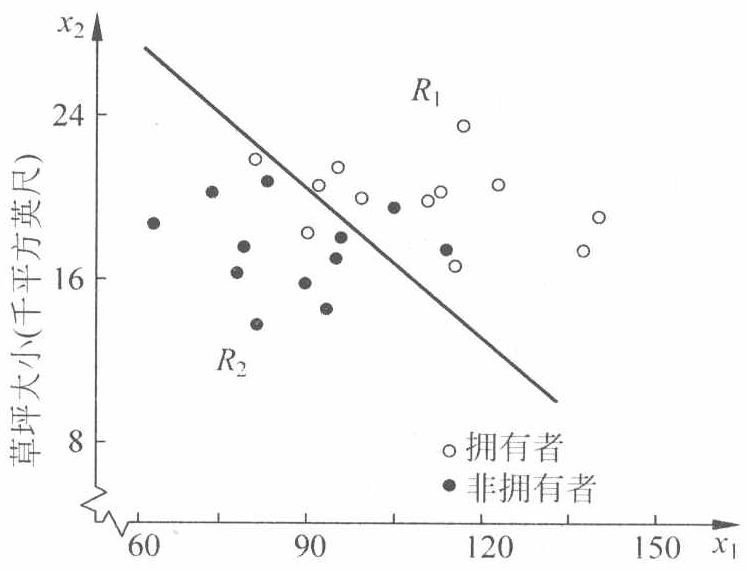
\includegraphics[width=63.2mm]{figs/fig_pg462_1.png}
\phantomsection\label{fig:11.1}\mvcap{图 11.1\quad 机动割草机的拥有者与非拥有者的收入和草坪大小}
\end{mvfigure}

%% ===== pg-463 =====

% ---- pg-463 （书页 451） ----

类. 换而言之, 错误分类的机会或概率应该很小. 我们将会看到, 一个“最优”分类法则还必须具备另外一些特性.

可能有这样的情况: 某一个类别或总体比另一个类别有更大的出现概率, 因为两个总体中一个比另一个大得多. 例如, 通常财务上健康的企业要大大多于濒临破产的企业. 另一个例子是: 某一类鸢尾比另一类更常见. 一个最优法则则应该考虑这些“先验出现概率”. 如果我们确信财务困难且最终将破产的企业的出现(先验)概率非常小, 就应将一个随机选取的企业分类为非破产的, 除非数据压倒性地倾向于破产.

分类的另一个问题是代价. 假如将一个 $\pi_1$ 对象误分为 $\pi_2$ 同将一个 $\pi_2$ 对象分入 $\pi_1$ 相比是一个更严重的错误, 那么我们就应对前者更加谨慎. 作为一个例子, 未能诊断出某种致命的疾病比错误地诊断有病(而实际上没有)是更严重的错误. 在任何可能的情况下, 最优分类方法应考虑与错误分类相联系的代价.

设 $f_1(\mathbf{x})$ 与 $f_2(\mathbf{x})$ 为 $p\times1$ 向量随机变量 $\mathbf{X}$ 分别在总体 $\pi_1$ 和 $\pi_2$ 中的概率密度函数. 设 $\Omega$ 为样本空间——所有可能的观测值 $\mathbf{x}$ 的集合. 一个具有观测值 $\mathbf{x}$ 的对象必须被指定属于 $\pi_1$ 或 $\pi_2$. 令 $R_1$ 为 $\mathbf{x}$ 值的一个集合, 当 $\mathbf{x}$ 属于 $R_1$ 时, 我们把对象分类为 $\pi_1$; $R_2=\Omega-R_1$ 为剩余的 $\mathbf{x}$ 值的集合, 对这些 $\mathbf{x}$ 值, 我们把对象分类为 $\pi_2$. 由于任一对象必定属于且只属于 $\pi_1$ 和 $\pi_2$ 之一, 因此 $R_1$ 和 $R_2$ 互斥且穷尽所有可能性. 对 $p=2$, 我们可能有形如\hyperref[fig:11.2]{图 11.2} 所示的情况.

\begin{mvfigure}
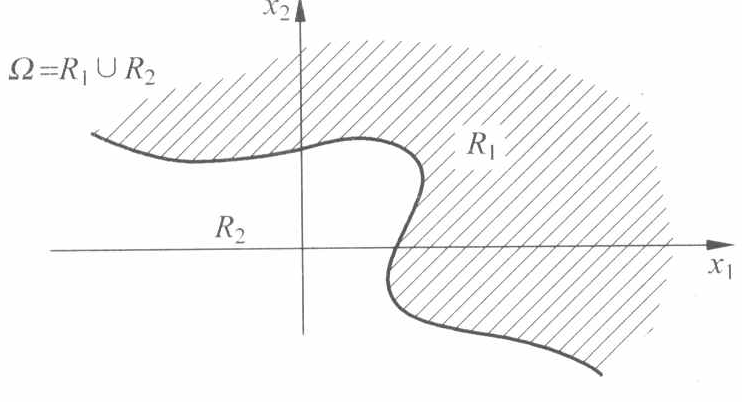
\includegraphics[width=62.8mm]{figs/fig_pg463_1.png}
\phantomsection\label{fig:11.2}\mvcap{图 11.2\quad 两个总体的分类区域}
\end{mvfigure}

将 $\pi_1$ 中的对象错分到 $\pi_2$ 的条件概率 $P(2\mid1)$ 为:
\phantomsection\label{eq:11-1}
\begin{equation}
P(2\mid1)=P(\mathbf{X}\in R_2\mid\pi_1)=\int_{R_2=\Omega-R_1}f_1(\mathbf{x})d\mathbf{x}
\tag{11-1}
\end{equation}
类似地, 将 $\pi_2$ 中的对象错分到 $\pi_1$ 的条件概率 $P(1\mid2)$ 为:
\phantomsection\label{eq:11-2}
\begin{equation}
P(1\mid2)=P(\mathbf{X}\in R_1\mid\pi_2)=\int_{R_1}f_2(\mathbf{x})d\mathbf{x}
\tag{11-2}
\end{equation}
在\hyperref[eq:11-1]{式(11-1)}中, 积分符号表示由密度函数 $f_1(\mathbf{x})$ 在区域 $R_2$ 中所形成的体积. 类似的, \hyperref[eq:11-2]{式(11-2)}中的积分符号表示由 $f_2(\mathbf{x})$ 在区域 $R_1$ 中所形成的体积. \hyperref[fig:11.3]{图 11.3} 在单变量($p=1$)场合对此作了说明.

\begin{mvfigure}
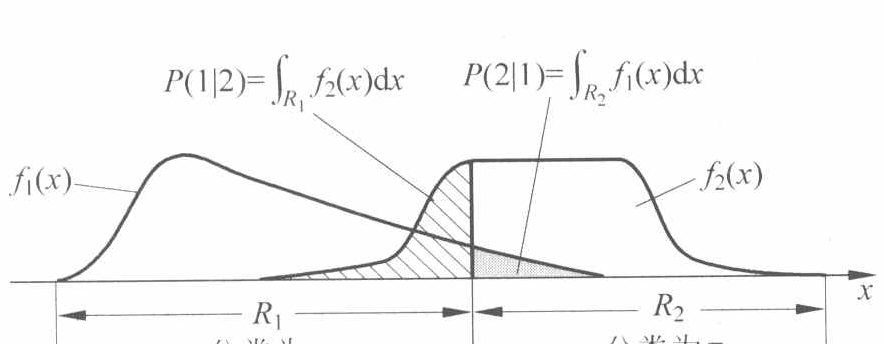
\includegraphics[width=74.8mm]{figs/fig_pg463_2.png}
\phantomsection\label{fig:11.3}\mvcap{图 11.3\quad 对假想分类区域的错分概率($p=1$)}
\end{mvfigure}

令 $p_1$ 为 $\pi_1$ 的先验概率, $p_2$ 为 $\pi_2$ 的先验概率, $p_1+p_2=1$. 此时正确或错误地将对象分类的无条件概率可表示为先验概率与条件概率之积:

%% ===== pg-464 =====

% ---- pg-464 （书页 452） ----

\phantomsection\label{eq:11-3}
\begin{equation}
\begin{aligned}
&P(\text{观测对象被正确地划入 }\pi_1)\\
&\quad =P(\text{观测对象来自 }\pi_1\text{, 且被划入 }\pi_1)\\
&\quad =P(\mathbf{X}\in R_1\mid\pi_1)P(\pi_1)=P(1\mid1)p_1\\[6pt]
&P(\text{观测对象被错误地划入 }\pi_1)\\
&\quad =P(\text{观测对象来自 }\pi_2\text{, 却被划入 }\pi_1)\\
&\quad =P(\mathbf{X}\in R_1\mid\pi_2)P(\pi_2)=P(1\mid2)p_2\\[6pt]
&P(\text{观测对象被正确地划入 }\pi_2)\\
&\quad =P(\text{观测对象来自 }\pi_2\text{, 且被划入 }\pi_2)\\
&\quad =P(\mathbf{X}\in R_2\mid\pi_2)P(\pi_2)=P(2\mid2)p_2\\[6pt]
&P(\text{观测对象被错误地划入 }\pi_2)\\
&\quad =P(\text{观测对象来自 }\pi_1\text{, 却被划入 }\pi_2)\\
&\quad =P(\mathbf{X}\in R_2\mid\pi_1)P(\pi_1)=P(2\mid1)p_1
\end{aligned}
\tag{11-3}
\end{equation}

分类方案经常按错分概率来评估(见 11.4 节), 但这样做忽视了错分的代价. 例如, 如果错分入 $\pi_1$ 的成本极其高昂, 那么即使像 $0.06=P(2\mid1)$ 这样的小概率也可能太大. 因此忽视代价的法则有可能引起问题.

错分代价可以用代价矩阵来定义:

\phantomsection\label{eq:11-4}
\begin{equation}
\begin{array}{r:c:c}
 & \multicolumn{2}{c}{\text{分类为:}}\\ \hdashline
\text{真实总体:} & \pi_1 & \pi_2\\ \hdashline
\pi_1 & 0 & c(2\mid1)\\
\pi_2 & c(1\mid2) & 0
\end{array}
\tag{11-4}
\end{equation}

(1)正确分类的代价为 0; (2)将属于 $\pi_2$ 的对象错分为 $\pi_1$ 的代价为 $c(1\mid2)$; (3)将属于 $\pi_1$ 的对象错分为 $\pi_2$ 的代价为 $c(2\mid1)$.

对任一法则, 平均的或期望的错分代价(ECM)可由\hyperref[eq:11-4]{式(11-4)}中的非对角元与错分概率乘积之和得到. 因此,

\phantomsection\label{eq:11-5}
\begin{equation}
\mathrm{ECM}=c(2\mid1)P(2\mid1)p_1+c(1\mid2)P(1\mid2)p_2
\tag{11-5}
\end{equation}

一个合理的分类法则应该有最小或尽可能小的 ECM.

\noindent\textbf{结论 11.1}\quad 使 ECM 达到最小的区域 $R_1$ 和 $R_2$ 由满足以下不等式的 $\mathbf{x}$ 值所定义:

\phantomsection\label{eq:11-6}
\begin{equation}
\begin{aligned}
R_1:\quad \frac{f_1(\mathbf{x})}{f_2(\mathbf{x})}&>\left(\frac{c(1\mid2)}{c(2\mid1)}\right)\left(\frac{p_2}{p_1}\right)\\
&(\text{密度比})\geqslant(\text{代价比})(\text{先验概率比})\\[6pt]
R_2:\quad \frac{f_1(\mathbf{x})}{f_2(\mathbf{x})}&<\left(\frac{c(1\mid2)}{c(2\mid1)}\right)\left(\frac{p_2}{p_1}\right)\\
&(\text{密度比})<(\text{代价比})(\text{先验概率比})
\end{aligned}
\tag{11-6}
\end{equation}

\noindent\mvbold{证明}\quad 见练习 11.3.\hfill$\blacksquare$

由\hyperref[eq:11-6]{式(11-6)}可以清楚看出, 建立最小 ECM 法则需要: (1) 在新观测值 $\mathbf{x}$ 处评估的密度函数比, (2) 代价比, 以及 (3) 先验概率比. 定义中出现的这些比值是有意义的, 因为在很多情况下, 确定这些比值往往比确定它们的组成部分要容易得多.

例如, 很难确定将一个事实上并非上大学材料的中学生划为是上大学材料的错划代价

%% ===== pg-465 =====

% ---- pg-465 （书页 453） ----

(取适当单位), 反之亦然. 例如, 对于纳税人, 教育一个在两年内就会退学的大学生的代价只能大致估计. 若大学和社会未能使一个有能力的学生受教育, 要估计这种代价更加困难. 然而, 对错分代价的比值却可能得出一个比较现实的数据. 无论取何种度量单位, 未录取一名有望读到毕业的大学生的代价可能 5 倍于录取一名最终退学的大学生的代价. 在这种场合, 代价比为 5.

有趣的是在某些特殊情形下考虑\hyperref[eq:11-6]{式(11-6)}所定义的分类区域.

\begin{mvframe}[最小期望代价域的几个特例]
\phantomsection\label{eq:11-7}
\begin{equation}
\begin{array}{l}
\text{(a) } p_2/p_1=1 \text{ (相同先验概率)}\\[4pt]
\qquad R_1:\ \dfrac{f_1(\mathbf{x})}{f_2(\mathbf{x})}\geqslant\dfrac{c(1\mid2)}{c(2\mid1)} \qquad R_2:\ \dfrac{f_1(\mathbf{x})}{f_2(\mathbf{x})}<\dfrac{c(1\mid2)}{c(2\mid1)}\\[8pt]
\text{(b) } c(1\mid2)/c(2\mid1)=1 \text{ (相同错分代价)}\\[4pt]
\qquad R_1:\ \dfrac{f_1(\mathbf{x})}{f_2(\mathbf{x})}\geqslant\dfrac{p_2}{p_1} \qquad R_2:\ \dfrac{f_1(\mathbf{x})}{f_2(\mathbf{x})}<\dfrac{p_2}{p_1}\\[8pt]
\text{(c) } p_2/p_1=c(1\mid2)/c(2\mid1)=1 \text{ 或 } p_2/p_1=1/(c(1\mid2)/c(2\mid1))\\
\qquad\text{(相同先验概率和相同错分代价)}\\[4pt]
\qquad R_1:\ \dfrac{f_1(\mathbf{x})}{f_2(\mathbf{x})}\geqslant 1 \qquad R_2:\ \dfrac{f_1(\mathbf{x})}{f_2(\mathbf{x})}<1
\end{array}
\tag{11-7}
\end{equation}
\end{mvframe}

当先验概率未知时, 它们通常被取成相等, 此时最小 ECM 法则只涉及总体密度比与适当的错分代价比的比较. 如果错分代价比不确定, 通常就取成 1, 结果就形成总体密度比与先验概率比的比较. 最后, 当先验概率比和错分代价比都是 1, 或者二者为倒数关系, 则最优分类区域就由比较总体密度的大小来决定. 在这种场合, 如果 $\mathbf{x}_0$ 是一个新的观测值, 且 $f_1(\mathbf{x}_0)/f_2(\mathbf{x}_0)\geqslant 1$, 即 $f_1(\mathbf{x}_0)\geqslant f_2(\mathbf{x}_0)$, 我们就将 $\mathbf{x}_0$ 分入 $\pi_1$. 反之, 若 $f_1(\mathbf{x}_0)/f_2(\mathbf{x}_0)<1$, 即 $f_1(\mathbf{x}_0)<f_2(\mathbf{x}_0)$, 我们就将 $\mathbf{x}_0$ 分入 $\pi_2$. 实践中一种普遍的做法是在分类时随意采用\hyperref[eq:11-7]{式(11-7)}中的情况(c). 这种做法等价于假定对最小 ECM 法则有相同的先验概率和相同的错分代价.\footnote{这是通常所提出的理由. 它也等价于假定先验概率比与错分代价比互为倒数.}

\noindent\textbf{例 11.2}\quad (将一个新的观测值分到两个总体之一)

某研究人员可获得足够的数据来估计分别与总体 $\pi_1$ 和 $\pi_2$ 相联系的密度函数 $f_1(\mathbf{x})$ 和 $f_2(\mathbf{x})$. 设 $c(2\mid1)=5$ 个单位, $c(1\mid2)=10$ 个单位. 此外, 已知大约 $20\%$ 的对象(所有这些对象的测量值均已取得)属于 $\pi_2$, 也就是说, 先验概率为 $p_1=0.8$, $p_2=0.2$.

给定先验概率和错分代价, 便可根据\hyperref[eq:11-6]{式(11-6)}导出分类区域 $R_1$ 和 $R_2$. 我们有
\[
R_1:\ \frac{f_1(\mathbf{x})}{f_2(\mathbf{x})}\geqslant\left(\frac{10}{5}\right)\times\left(\frac{0.2}{0.8}\right)=0.5
\]
\[
R_2:\ \frac{f_1(\mathbf{x})}{f_2(\mathbf{x})}<\left(\frac{10}{5}\right)\times\left(\frac{0.2}{0.8}\right)=0.5
\]

假定在一个新的观测点 $\mathbf{x}_0$ 算得 $f_1(\mathbf{x}_0)=0.3$ 和 $f_2(\mathbf{x}_0)=0.4$. 试问: 应将此新观测点分入 $\pi_1$ 还是 $\pi_2$? 为回答此问题, 我们计算比值
\[
\frac{f_1(\mathbf{x}_0)}{f_2(\mathbf{x}_0)}=\frac{0.3}{0.4}=0.75
\]
并将此值与前面得到的结果比较. 由于

%% ===== pg-466 =====

% ---- pg-466 （书页 454） ----

\[
\frac{f_1(\mathbf{x}_0)}{f_2(\mathbf{x}_0)}=0.75>\left(\frac{c(1\mid2)}{c(2\mid1)}\right)\left(\frac{p_2}{p_1}\right)=0.5
\]
我们发现 $\mathbf{x}_0\in R_1$, 因此将其分入 $\pi_1$.\hfill$\blacksquare$

用不同于期望错分代价的准则也能导出“最优”分类方法. 例如, 可以不考虑错分代价, 通过选择 $R_1$ 和 $R_2$ 使总错分概率(TPM)
\phantomsection\label{eq:11-8}
\begin{equation}
\begin{aligned}
\mathrm{TPM}&=P(\text{错分 }\pi_1\text{ 的观测值或错分 }\pi_2\text{ 的观测值})\\
&=P(\text{观测值来自 }\pi_1\text{, 但被错分入 }\pi_2)\\
&\quad +P(\text{观测值来自 }\pi_2\text{, 但被错分入 }\pi_1)\\
&=p_1\int_{R_2}f_1(\mathbf{x})\,\mathrm{d}\mathbf{x}+p_2\int_{R_1}f_2(\mathbf{x})\,\mathrm{d}\mathbf{x}
\end{aligned}
\tag{11-8}
\end{equation}
达到极小. 数学上, 这个问题等价于在错分代价相同的情况下使期望错分代价最小化. 因此, 这种情况下的最优区域由\hyperref[eq:11-7]{式(11-7)}中的(b)给出.

我们也可以按最大“后验”概率 $P(\pi_i\mid\mathbf{x}_0)$ 将新观测值 $\mathbf{x}_0$ 分配给总体. 根据贝叶斯法则, 后验概率为:
\phantomsection\label{eq:11-9}
\begin{equation}
\begin{aligned}
P(\pi_1\mid\mathbf{x}_0)&=\frac{P(\pi_1\text{ 发生和我们观察到 }\mathbf{x}_0)}{P(\text{我们观察到 }\mathbf{x}_0)}\\
&=\frac{P(\text{我们观察到 }\mathbf{x}_0\mid\pi_1)P(\pi_1)}{P(\text{我们观察到 }\mathbf{x}_0\mid\pi_1)P(\pi_1)+P(\text{我们观察到 }\mathbf{x}_0\mid\pi_2)P(\pi_2)}\\
&=\frac{p_1f_1(\mathbf{x}_0)}{p_1f_1(\mathbf{x}_0)+p_2f_2(\mathbf{x}_0)}\\
P(\pi_2\mid\mathbf{x}_0)&=1-P(\pi_1\mid\mathbf{x}_0)=\frac{p_2f_2(\mathbf{x}_0)}{p_1f_1(\mathbf{x}_0)+p_2f_2(\mathbf{x}_0)}
\end{aligned}
\tag{11-9}
\end{equation}
当 $P(\pi_1\mid\mathbf{x}_0)>P(\pi_2\mid\mathbf{x}_0)$ 时将观测值 $\mathbf{x}_0$ 分入 $\pi_1$, 这相当于采用\hyperref[eq:11-7]{式(11-7)}中的总错分概率的法则(b), 因为\hyperref[eq:11-9]{式(11-9)}中两式的分母相同. 但是, 在观测到 $\mathbf{x}_0$ 后再计算总体 $\pi_1$ 和 $\pi_2$ 的概率(因此名为后验概率), 这对识别不很明确的分配来说常常很有用.\hfill$\blacksquare$

\section{两个多元正态总体的分类}  % 原书 11.3
\phantomsection\label{sec:11.3}

在统计实践中, 基于正态总体的分类方法居主导地位. 这是因为对范围广阔的总体模型来说, 这些分类方法简单而高效. 现在我们假定 $f_1(\mathbf{x})$ 和 $f_2(\mathbf{x})$ 为多元正态密度, 分别具有均值向量 $\boldsymbol{\mu}_1$, 协方差矩阵 $\boldsymbol{\Sigma}_1$ 和均值向量 $\boldsymbol{\mu}_2$, 协方差矩阵 $\boldsymbol{\Sigma}_2$.

两个协方差矩阵相等的特殊情况导致特别简单的线性分类统计量.

\mvsub{当 \texorpdfstring{$\boldsymbol{\Sigma}_1=\boldsymbol{\Sigma}_2=\boldsymbol{\Sigma}$}{Sigma1=Sigma2=Sigma} 时正态总体的分类}

假定 $\mathbf{X}'=[X_1,X_2,\cdots,X_p]$ 对总体 $\pi_1$ 和 $\pi_2$ 的联合密度为
\phantomsection\label{eq:11-10}
\begin{equation}
f_i(\mathbf{x})=\frac{1}{(2\pi)^{p/2}|\boldsymbol{\Sigma}|^{1/2}}\exp\left[-\frac{1}{2}(\mathbf{x}-\boldsymbol{\mu}_i)'\boldsymbol{\Sigma}^{-1}(\mathbf{x}-\boldsymbol{\mu}_i)\right]\qquad \text{对 } i=1,2
\tag{11-10}
\end{equation}
再假定总体参数 $\boldsymbol{\mu}_1$, $\boldsymbol{\mu}_2$ 和 $\boldsymbol{\Sigma}$ 皆已知. 此时在消去公因子 $(2\pi)^{p/2}|\boldsymbol{\Sigma}|^{1/2}$ 后, \hyperref[eq:11-6]{式(11-6)}中的最小 ECM 区域变成:
\[
\begin{aligned}
R_1:\ \exp&\left[-\frac{1}{2}(\mathbf{x}-\boldsymbol{\mu}_1)'\boldsymbol{\Sigma}^{-1}(\mathbf{x}-\boldsymbol{\mu}_1)+\frac{1}{2}(\mathbf{x}-\boldsymbol{\mu}_2)'\boldsymbol{\Sigma}^{-1}(\mathbf{x}-\boldsymbol{\mu}_2)\right]\\
&\geqslant\left(\frac{c(1\mid2)}{c(2\mid1)}\right)\left(\frac{p_2}{p_1}\right)
\end{aligned}
\]

%% ===== pg-467 =====

% ---- pg-467 （书页 455） ----

\phantomsection\label{eq:11-11}
\begin{equation}
\begin{aligned}
R_2:\ \exp&\left[-\frac{1}{2}(\mathbf{x}-\boldsymbol{\mu}_1)'\boldsymbol{\Sigma}^{-1}(\mathbf{x}-\boldsymbol{\mu}_1)+\frac{1}{2}(\mathbf{x}-\boldsymbol{\mu}_2)'\boldsymbol{\Sigma}^{-1}(\mathbf{x}-\boldsymbol{\mu}_2)\right]\\
&<\left(\frac{c(1\mid2)}{c(2\mid1)}\right)\left(\frac{p_2}{p_1}\right)
\end{aligned}
\tag{11-11}
\end{equation}

给定这些区域 $R_1$ 和 $R_2$, 我们就可以构造下述结论中给出的分类法则.

\noindent\textbf{结论 11.2}\quad 设总体 $\pi_1$ 和 $\pi_2$ 由形如\hyperref[eq:11-10]{式(11-10)}的多元正态密度描述. 此时能使 ECM 最小化的分配法则如下:

当
\phantomsection\label{eq:11-12}
\begin{equation}
(\boldsymbol{\mu}_1-\boldsymbol{\mu}_2)'\boldsymbol{\Sigma}^{-1}\mathbf{x}_0-\frac{1}{2}(\boldsymbol{\mu}_1-\boldsymbol{\mu}_2)'\boldsymbol{\Sigma}^{-1}(\boldsymbol{\mu}_1+\boldsymbol{\mu}_2)\geqslant\ln\left[\left(\frac{c(1\mid2)}{c(2\mid1)}\right)\left(\frac{p_2}{p_1}\right)\right]
\tag{11-12}
\end{equation}
时将 $\mathbf{x}_0$ 分配给 $\pi_1$, 否则将 $\mathbf{x}_0$ 分配给 $\pi_2$.

\noindent\mvbold{证明}\quad 由于对所有 $\mathbf{x}$, \hyperref[eq:11-11]{式(11-11)}中的量均属非负, 我们可以取它们的自然对数, 同时保持不等号不变. 进一步有(见练习 11.5),
\phantomsection\label{eq:11-13}
\begin{equation}
\begin{aligned}
&-\frac{1}{2}(\mathbf{x}-\boldsymbol{\mu}_1)'\boldsymbol{\Sigma}^{-1}(\mathbf{x}-\boldsymbol{\mu}_1)+\frac{1}{2}(\mathbf{x}-\boldsymbol{\mu}_2)'\boldsymbol{\Sigma}^{-1}(\mathbf{x}-\boldsymbol{\mu}_2)\\
&\quad =(\boldsymbol{\mu}_1-\boldsymbol{\mu}_2)'\boldsymbol{\Sigma}^{-1}\mathbf{x}-\frac{1}{2}(\boldsymbol{\mu}_1-\boldsymbol{\mu}_2)'\boldsymbol{\Sigma}^{-1}(\boldsymbol{\mu}_1+\boldsymbol{\mu}_2)
\end{aligned}
\tag{11-13}
\end{equation}
于是
\phantomsection\label{eq:11-14}
\begin{equation}
\begin{aligned}
R_1:\ &(\boldsymbol{\mu}_1-\boldsymbol{\mu}_2)'\boldsymbol{\Sigma}^{-1}\mathbf{x}-\frac{1}{2}(\boldsymbol{\mu}_1-\boldsymbol{\mu}_2)'\boldsymbol{\Sigma}^{-1}(\boldsymbol{\mu}_1+\boldsymbol{\mu}_2)\geqslant\ln\left[\left(\frac{c(1\mid2)}{c(2\mid1)}\right)\left(\frac{p_2}{p_1}\right)\right]\\
R_2:\ &(\boldsymbol{\mu}_1-\boldsymbol{\mu}_2)'\boldsymbol{\Sigma}^{-1}\mathbf{x}-\frac{1}{2}(\boldsymbol{\mu}_1-\boldsymbol{\mu}_2)'\boldsymbol{\Sigma}^{-1}(\boldsymbol{\mu}_1+\boldsymbol{\mu}_2)<\ln\left[\left(\frac{c(1\mid2)}{c(2\mid1)}\right)\left(\frac{p_2}{p_1}\right)\right]
\end{aligned}
\tag{11-14}
\end{equation}
这样就证明了结论 11.2.\hfill$\blacksquare$

在大多数实际情况下, 总体参数 $\boldsymbol{\mu}_1$, $\boldsymbol{\mu}_2$ 和 $\boldsymbol{\Sigma}$ 均为未知系数, 因此法则(11-12)必须修改. 沃尔德(Wald, 见文献[31])和安德森(Anderson, 见文献[2])建议将总体参数用它们的样本对应量来代替.

然后, 假定多元随机变量 $\mathbf{X}'=[X_1,X_2,\cdots,X_p]$ 有 $n_1$ 个观测值来自 $\pi_1$ 和 $n_2$ 个观测值来自 $\pi_2$, $n_1+n_2-2\geqslant p$. 这时相应的数据矩阵分别为
\phantomsection\label{eq:11-15}
\begin{equation}
\underset{(n_1\times p)}{\mathbf{X}_1}=\begin{bmatrix}\mathbf{x}_{11}'\\\mathbf{x}_{12}'\\\vdots\\\mathbf{x}_{1n_1}'\end{bmatrix},\qquad \underset{(n_2\times p)}{\mathbf{X}_2}=\begin{bmatrix}\mathbf{x}_{21}'\\\mathbf{x}_{22}'\\\vdots\\\mathbf{x}_{2n_2}'\end{bmatrix}
\tag{11-15}
\end{equation}

根据这些数据矩阵, 样本均值向量和样本协方差矩阵由下列诸式确定:
\phantomsection\label{eq:11-16}
\begin{equation}
\begin{aligned}
\underset{(p\times1)}{\bar{\mathbf{x}}_1}&=\frac{1}{n_1}\sum_{j=1}^{n_1}\mathbf{x}_{1j}, & \underset{(p\times p)}{\mathbf{S}_1}&=\frac{1}{n_1-1}\sum_{j=1}^{n_1}(\mathbf{x}_{1j}-\bar{\mathbf{x}}_1)(\mathbf{x}_{1j}-\bar{\mathbf{x}}_1)'\\
\underset{(p\times1)}{\bar{\mathbf{x}}_2}&=\frac{1}{n_2}\sum_{j=1}^{n_2}\mathbf{x}_{2j}, & \underset{(p\times p)}{\mathbf{S}_2}&=\frac{1}{n_2-1}\sum_{j=1}^{n_2}(\mathbf{x}_{2j}-\bar{\mathbf{x}}_2)(\mathbf{x}_{2j}-\bar{\mathbf{x}}_2)'
\end{aligned}
\tag{11-16}
\end{equation}

由于假定总体有相同的协方差矩阵 $\boldsymbol{\Sigma}$, 样本协方差矩阵 $\mathbf{S}_1$ 和 $\mathbf{S}_2$ 应联合起来, 以导出一个如\hyperref[eq:6-21]{式(6-21)}那样的 $\boldsymbol{\Sigma}$ 的无偏估计. 特别是, 如果数据矩阵 $\mathbf{X}_1$ 和 $\mathbf{X}_2$ 分别包含来自总体 $\pi_1$ 和 $\pi_2$ 的随机样本, 则加权平均
\phantomsection\label{eq:11-17}
\begin{equation}
\mathbf{S}_{\mathrm{p}}=\left[\frac{n_1-1}{(n_1-1)+(n_2-1)}\right]\mathbf{S}_1+\left[\frac{n_2-1}{(n_1-1)+(n_2-1)}\right]\mathbf{S}_2
\tag{11-17}
\end{equation}

%% ===== pg-468 =====

% ---- pg-468 （书页 456） ----

便是 $\boldsymbol{\Sigma}$ 的一个无偏估计.

在\hyperref[eq:11-12]{式(11-12)}中, 用 $\bar{\mathbf{x}}_1$ 代替 $\boldsymbol{\mu}_1$, $\bar{\mathbf{x}}_2$ 代替 $\boldsymbol{\mu}_2$, $\mathbf{S}_{\mathrm{p}}$ 代替 $\boldsymbol{\Sigma}$, 就得到“样本”分类法则:

\begin{mvframe}[两个正态总体的估计的最小 ECM 法则]
若
\phantomsection\label{eq:11-18}
\begin{equation}
(\bar{\mathbf{x}}_1-\bar{\mathbf{x}}_2)'\mathbf{S}_{\mathrm{p}}^{-1}\mathbf{x}_0-\frac{1}{2}(\bar{\mathbf{x}}_1-\bar{\mathbf{x}}_2)'\mathbf{S}_{\mathrm{p}}^{-1}(\bar{\mathbf{x}}_1+\bar{\mathbf{x}}_2)\geqslant\ln\left[\left(\frac{c(1\mid2)}{c(2\mid1)}\right)\left(\frac{p_2}{p_1}\right)\right]
\tag{11-18}
\end{equation}
则分配 $\mathbf{x}_0$ 到 $\pi_1$, 否则分配 $\mathbf{x}_0$ 到 $\pi_2$.
\end{mvframe}

若在\hyperref[eq:11-18]{式(11-18)}中
\[
\left(\frac{c(1\mid2)}{c(2\mid1)}\right)\left(\frac{p_2}{p_1}\right)=1
\]
则 $\ln(1)=0$, 因此两个正态总体的估计的最小 ECM 法则等价于将在 $\mathbf{x}_0$ 点得出的标量
\phantomsection\label{eq:11-19}
\begin{equation}
\hat{y}=(\bar{\mathbf{x}}_1-\bar{\mathbf{x}}_2)'\mathbf{S}_{\mathrm{p}}^{-1}\mathbf{x}=\hat{\mathbf{a}}'\mathbf{x}
\tag{11-19}
\end{equation}
与数字
\phantomsection\label{eq:11-20}
\begin{equation}
\begin{aligned}
\hat{m}&=\frac{1}{2}(\bar{\mathbf{x}}_1-\bar{\mathbf{x}}_2)'\mathbf{S}_{\mathrm{p}}^{-1}(\bar{\mathbf{x}}_1+\bar{\mathbf{x}}_2)\\
&=\frac{1}{2}(\hat{y}_1+\hat{y}_2)
\end{aligned}
\tag{11-20}
\end{equation}
作比较, 其中
\[
\begin{aligned}
\hat{y}_1&=(\bar{\mathbf{x}}_1-\bar{\mathbf{x}}_2)'\mathbf{S}_{\mathrm{p}}^{-1}\bar{\mathbf{x}}_1=\hat{\mathbf{a}}'\bar{\mathbf{x}}_1\\
\hat{y}_2&=(\bar{\mathbf{x}}_1-\bar{\mathbf{x}}_2)'\mathbf{S}_{\mathrm{p}}^{-1}\bar{\mathbf{x}}_2=\hat{\mathbf{a}}'\bar{\mathbf{x}}_2
\end{aligned}
\]

也就是说, 两正态总体的估计的最小 ECM 法则等价于建立两个单变量总体 $y_1, y_2$ 为来自总体 $\pi_1$ 和 $\pi_2$ 的观测值的适当线性组合, 然后根据 $\hat{y}_0=\hat{\mathbf{a}}'\mathbf{x}_0$ 落在 $\hat{y}_1$ 和 $\hat{y}_2$ 的连线中点 $\hat{m}$ 的右侧还是左侧来决定将新的观测值 $\mathbf{x}_0$ 分到 $\pi_1$ 还是 $\pi_2$.

一旦总体未知参数用其估计值代替, 就无法保证所得出的法则在具体应用中能使 ECM 最小化. 这是因为\hyperref[eq:11-12]{式(11-12)}中的最优法则是在假定多元正态密度 $f_1(\mathbf{x})$ 和 $f_2(\mathbf{x})$ 完全已知的前提下导出的, 而\hyperref[eq:11-18]{式(11-18)}只是最优法则的一个估计. 然而, 如果样本容量大, 就有理由期望这个估计有良好表现.\footnote{当样本容量增加时, $\bar{x}_1$, $\bar{x}_2$ 和 $\mathbf{S}_{\mathrm{p}}$ 以接近于 1 的概率变得分别与 $\boldsymbol{\mu}_1$, $\boldsymbol{\mu}_2$ 和 $\boldsymbol{\Sigma}$ 无法区分[见\hyperref[eq:4-26]{式(4-26)}和\hyperref[eq:4-27]{式(4-27)}].}

归纳起来, 如果数据表现为多元正态分布\footnote{至少对每个变量来说, 其观测值的边际频数分布的正态性是可以检验的. 此项工作对来自两个总体的样本都要做. 经常需要将某些变量作适当的变换, 以使它们更“像正态变量”(见 4.6 节和 4.8 节).}, 则对每一个新的观测值, $\mathbf{x}_0$ 可以计算\hyperref[eq:11-18]{式(11-18)}左端的分类统计量. 这些观测值可通过比较这个统计量的值与 $\ln[(c(1\mid2)/c(2\mid1))(p_2/p_1)]$ 的值来分类.

\noindent\textbf{例 11.3}\quad (两正态总体有共同$\boldsymbol{\Sigma}$与相同代价情况下的分类)

本例的材料来自一项有关查明带 A 型血友病基因者的研究(见文献[4], 同时参见练习 11.32).

为构造一个查明带 A 型血友病基因者的方法, 研究人员分析了两组女性的血样, 并记录

%% ===== pg-469 =====

% ---- pg-469 （书页 457） ----

了以下两个变量:
\[
\begin{aligned}
X_1&=\log_{10}(\text{AHF 活性})\\
X_2&=\log_{10}(\text{类 AHF 抗原})
\end{aligned}
\]
(“AHF”代表“抗血友病因子”.) 第一组妇女共 $n_1=30$ 人, 来自不携带血友病基因的女性总体. 这个组称为正常组. 第二组有 $n_2=22$ 个妇女, 来自已知的 A 型血友病患者总体(血友病患者的女儿, 有多于一个血友病儿子的母亲, 以及有一个血友病儿子且有其他血友病亲戚的母亲). 这一组称为必然携带者. 这两组观测值对 $(x_1,x_2)$ 示于\hyperref[fig:11.4]{图 11.4}. 图中还分别展示了对二元正态分布(以 $\bar{\mathbf{x}}_1$ 和 $\bar{\mathbf{x}}_2$ 为中心)含 $50\%$ 和 $95\%$ 概率的估计轮廓线. 两个总体共同的协方差矩阵用联合样本协方差矩阵 $\mathbf{S}_{\mathrm{p}}$ 来估计. 在本例中, 二元正态分布看来同数据拟合得相当好.

\begin{mvfigure}
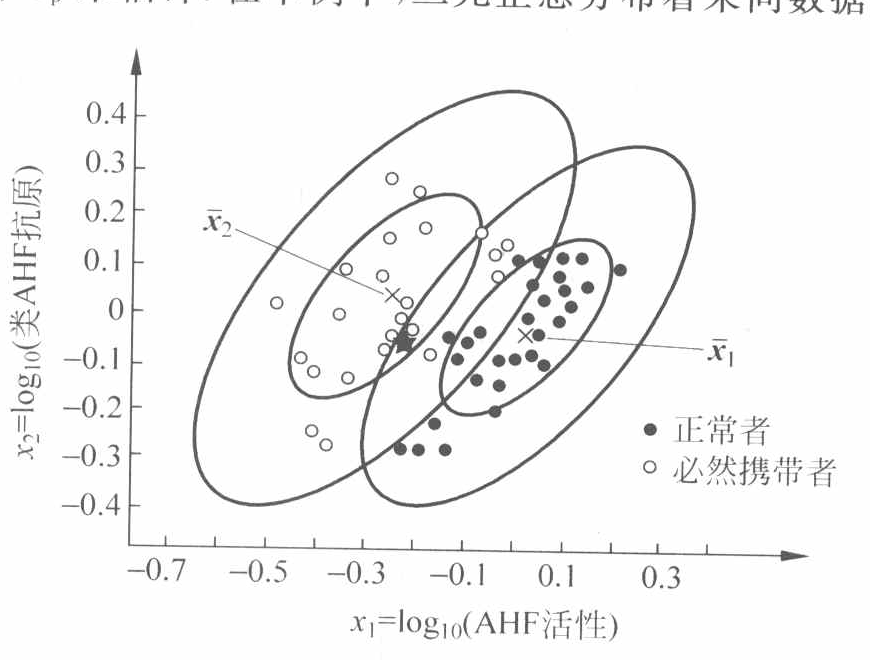
\includegraphics[width=73.6mm]{figs/fig_pg469_1.png}
\phantomsection\label{fig:11.4}\mvcap{图 11.4\quad 血友病数据的散布图}
\end{mvfigure}

研究人员(见文献[4])提供了下列信息:
\[
\bar{\mathbf{x}}_1=\begin{bmatrix}-0.006\,5\\-0.039\,0\end{bmatrix},\qquad \bar{\mathbf{x}}_2=\begin{bmatrix}-0.248\,3\\0.026\,2\end{bmatrix}
\]
以及
\[
\mathbf{S}_{\mathrm{p}}^{-1}=\begin{bmatrix}131.158&-90.423\\-90.423&108.147\end{bmatrix}
\]
因此, 相同代价和相同先验概率的判别函数[见\hyperref[eq:11-19]{式(11-19)}]为
\[
\begin{aligned}
\hat{y}&=\hat{\mathbf{a}}'\mathbf{x}=[\bar{\mathbf{x}}_1-\bar{\mathbf{x}}_2]'\mathbf{S}_{\mathrm{p}}^{-1}\mathbf{x}\\
&=[0.241\,8\quad -0.065\,2]\begin{bmatrix}131.158&-90.423\\-90.423&108.147\end{bmatrix}\begin{bmatrix}x_1\\x_2\end{bmatrix}\\
&=37.61x_1-28.92x_2
\end{aligned}
\]
进而有
\[
\begin{aligned}
\hat{y}_1&=\hat{\mathbf{a}}'\bar{\mathbf{x}}_1=[37.61\quad -28.92]\begin{bmatrix}-0.006\,5\\-0.039\,0\end{bmatrix}=0.88\\
\hat{y}_2&=\hat{\mathbf{a}}'\bar{\mathbf{x}}_2=[37.61\quad -28.92]\begin{bmatrix}-0.248\,3\\0.026\,2\end{bmatrix}=-10.10
\end{aligned}
\]
因此均值连线的中点[见\hyperref[eq:11-20]{式(11-20)}]为
\[
\hat{m}=\frac{1}{2}(\hat{y}_1+\hat{y}_2)=\frac{1}{2}\times(0.88-10.10)=-4.61
\]

%% ===== pg-470 =====

% ---- pg-470 （书页 458） ----

假定查得另一个妇女的两个变量值为 $x_1=-0.210$ 和 $x_2=-0.044$, 这个妇女应被分入 $\pi_1$(正常组)还是 $\pi_2$(必然携带组)?

利用\hyperref[eq:11-18]{式(11-18)}, 并设有相同的代价和相同的先验概率(故 $\ln 1=0$), 就有
\[
\begin{aligned}
&\text{分配 } \mathbf{x}_0 \text{ 到 } \pi_1, \text{若 } \hat{y}_0=\hat{\mathbf{a}}'\mathbf{x}_0\geqslant\hat{m}=-4.61\\[4pt]
&\text{分配 } \mathbf{x}_0 \text{ 到 } \pi_2, \text{若 } \hat{y}_0=\hat{\mathbf{a}}'\mathbf{x}_0<\hat{m}=-4.61
\end{aligned}
\]
这里 $\mathbf{x}_0'=(-0.210,-0.044)$. 由于
\[
\hat{y}_0=\hat{\mathbf{a}}'\mathbf{x}_0=[37.61\quad -28.92]\begin{bmatrix}-0.210\\-0.044\end{bmatrix}=-6.62<-4.61
\]
因此将她分入 $\pi_2$, 即这位妇女是 A 型血友病基因的必然携带者. 这个新的观测点在\hyperref[fig:11.4]{图 11.4} 中用一个星号表示. 从图上可以看到, 这个点落在 $\pi_2$ 的 $50\%$ 轮廓线内, 而大体位于 $\pi_1$ 的 $95\%$ 轮廓线上. 这样, 分类就不是很明确.

现在假定组成员的先验概率已知. 例如, 假定产生上述测量值 $x_1$ 和 $x_2$ 的血液来自一个血友病患者的外甥, 这时她的基因具有 A 型血友病缺陷的机会为 0.25. 因此 $\pi_1$ 的先验概率为 $p_1=0.75$, 而 $\pi_2$ 的先验概率为 $p_2=0.25$. 假定错分代价相同, 即 $c(1\mid2)=c(2\mid1)$, 并使用分类统计量
\[
\hat{w}=(\bar{\mathbf{x}}_1-\bar{\mathbf{x}}_2)'\mathbf{S}_{\mathrm{p}}^{-1}\mathbf{x}_0-\frac{1}{2}(\bar{\mathbf{x}}_1-\bar{\mathbf{x}}_2)'\mathbf{S}_{\mathrm{p}}^{-1}(\bar{\mathbf{x}}_1+\bar{\mathbf{x}}_2)
\]
或 $\hat{w}=\hat{\mathbf{a}}'\mathbf{x}_0-\hat{m}$, 其中 $\mathbf{x}_0'=[-0.210,-0.044]$, $\hat{m}=-4.61$, 以及 $\hat{\mathbf{a}}'\mathbf{x}_0=-6.62$, 我们有
\[
\hat{w}=-6.62-(-4.61)=-2.01
\]
应用\hyperref[eq:11-18]{式(11-18)}, 得到
\[
\hat{w}=-2.01<\ln\left[\frac{p_2}{p_1}\right]=\ln\left[\frac{0.25}{0.75}\right]=-1.10
\]
因此我们将此妇女分入 $\pi_2$(必然携带者).\hfill$\blacksquare$

\mvsub{刻度变换}

系数向量 $\hat{\mathbf{a}}=\mathbf{S}_{\mathrm{p}}^{-1}(\bar{\mathbf{x}}_1-\bar{\mathbf{x}}_2)$ 只是在相差一个常数因子的意义上唯一, 因此对 $c\neq0$, 任一向量 $c\hat{\mathbf{a}}$ 均可成为判别系数.

向量 $\hat{\mathbf{a}}$ 经常被“刻度变换”或“规范化”, 以便于解释其元素. 两种最常用的规范化方法为:

1. 令
\phantomsection\label{eq:11-21}
\begin{equation}
\hat{\mathbf{a}}^*=\frac{\hat{\mathbf{a}}}{\sqrt{\hat{\mathbf{a}}'\hat{\mathbf{a}}}}
\tag{11-21}
\end{equation}
因此 $\hat{\mathbf{a}}^*$ 具有单位长度.

2. 令
\phantomsection\label{eq:11-22}
\begin{equation}
\hat{\mathbf{a}}^*=\frac{\hat{\mathbf{a}}}{\hat{a}_1}
\tag{11-22}
\end{equation}
因此新的系数向量 $\hat{\mathbf{a}}^*$ 的第一个元素为 1.

在以上两种场合, $\hat{\mathbf{a}}^*$ 均具有形式 $c\hat{\mathbf{a}}$. 对规范化(1)有 $c=(\hat{\mathbf{a}}'\hat{\mathbf{a}})^{-1/2}$, 而对(2)有 $c=\hat{a}_1^{-1}$.

%% ===== pg-471 =====

% ---- pg-471 （书页 459） ----

在\hyperref[eq:11-21]{式(11-21)}中, $\hat{a}_1^*, \hat{a}_2^*, \cdots, \hat{a}_p^*$ 的值都落在区间 $[-1,1]$ 之内. 在\hyperref[eq:11-22]{式(11-22)}中, $\hat{a}_1^*=1$, 而 $\hat{a}_2^*, \cdots, \hat{a}_p^*$ 表示为 $\hat{a}_1^*$ 的倍数. 将 $\hat{a}_i^*$ 约束在区间 $[-1,1]$ 内, 有利于对系数进行直观比较. 类似的, 将 $\hat{a}_i^*$ 表示为 $\hat{a}_1^*$ 的倍数有利于评估变量 $X_2,\cdots,X_p$ 作为判别量的相对重要性(相对于 $X_1$).

只有当 $X$ 变量经过标准化之后, 我们才建议将 $\hat{a}_i$ 规范化. 如果不是这种情况, 在解释分析结果时就必须非常小心.

\mvsub{费希尔判别函数——分离总体}

费希尔(见文献[10])实际上是根据一个完全不同的论据发现\hyperref[eq:11-19]{式(11-19)}所给的分类统计量的. 他的想法是将多元观测值 $\mathbf{x}$ 变换成一元观测值 $y$, 使得由总体 $\pi_1$ 和 $\pi_2$ 导出的 $y$ 尽可能地分离开. 费希尔建议用 $\mathbf{x}$ 的线性组合来建立 $y$, 因为它们是 $\mathbf{x}$ 的非常简单的函数, 易于掌握. 费希尔的方法并未假定总体具有正态性, 但是隐含有总体协方差矩阵相等的假定, 因为使用了公共协方差矩阵的联合估计量.

假定 $\mathbf{x}$ 的一个固定线性组合对来自第一个总体的观测值来说其取值为 $y_{11},y_{12},\cdots,y_{1n_1}$, 对来自第二个总体的观测值来说其取值为 $y_{21},y_{22},\cdots,y_{2n_2}$. 这两组单变量数据之间的分离度用以标准差为单位的 $\bar{y}_1$ 与 $\bar{y}_2$ 之间的差别来表示, 即
\[
\text{分离度}=\frac{|\bar{y}_1-\bar{y}_2|}{s_y},\qquad \text{其中 } s_y^2=\frac{\sum_{j=1}^{n_1}(y_{1j}-\bar{y}_1)^2+\sum_{j=1}^{n_2}(y_{2j}-\bar{y}_2)^2}{n_1+n_2-2}
\]
为方差的联合估计量. 目标是选择适当的 $\mathbf{x}$ 的线性组合, 使得样本均值 $\bar{y}_1$ 与 $\bar{y}_2$ 之间的分离度达到最大.

\noindent\textbf{结论 11.3}\quad 线性组合 $\hat{y}=\hat{\mathbf{a}}'\mathbf{x}=(\bar{\mathbf{x}}_1-\bar{\mathbf{x}}_2)'\mathbf{S}_{\mathrm{p}}^{-1}\mathbf{x}$ 对所有可能的线性系数向量 $\hat{\mathbf{a}}$ 使下述比值达到最大:
\phantomsection\label{eq:11-23}
\begin{equation}
\begin{aligned}
\frac{(y\text{ 的样本均值之间的距离平方})}{(y\text{ 的样本方差})}&=\frac{(\bar{y}_1-\bar{y}_2)^2}{s_y^2}\\
&=\frac{(\hat{\mathbf{a}}'\bar{\mathbf{x}}_1-\hat{\mathbf{a}}'\bar{\mathbf{x}}_2)^2}{\hat{\mathbf{a}}'\mathbf{S}_{\mathrm{p}}\hat{\mathbf{a}}}\\
&=\frac{(\hat{\mathbf{a}}'\mathbf{d})^2}{\hat{\mathbf{a}}'\mathbf{S}_{\mathrm{p}}\hat{\mathbf{a}}}
\end{aligned}
\tag{11-23}
\end{equation}
其中 $\mathbf{d}=(\bar{\mathbf{x}}_1-\bar{\mathbf{x}}_2)$. 比值(11-23)的最大值为 $D^2=(\bar{\mathbf{x}}_1-\bar{\mathbf{x}}_2)'\mathbf{S}_{\mathrm{p}}^{-1}(\bar{\mathbf{x}}_1-\bar{\mathbf{x}}_2)$.

\noindent\mvbold{证明}\quad 比值(11-23)的最大值直接由\hyperref[eq:2-50]{式(2-50)}给出. 这样, 令 $\mathbf{d}=(\bar{\mathbf{x}}_1-\bar{\mathbf{x}}_2)$, 就有
\[
\max_{\hat{\mathbf{a}}}\frac{(\hat{\mathbf{a}}'\mathbf{d})^2}{\hat{\mathbf{a}}'\mathbf{S}_{\mathrm{p}}\hat{\mathbf{a}}}=\mathbf{d}'\mathbf{S}_{\mathrm{p}}^{-1}\mathbf{d}=(\bar{\mathbf{x}}_1-\bar{\mathbf{x}}_2)'\mathbf{S}_{\mathrm{p}}^{-1}(\bar{\mathbf{x}}_1-\bar{\mathbf{x}}_2)=D^2
\]
其中 $D^2$ 为两个均值之间的样本平方距离.\hfill$\blacksquare$

注意, \hyperref[eq:11-23]{式(11-23)}中的 $s_y^2$ 可按下式计算:
\phantomsection\label{eq:11-24}
\begin{equation}
s_y^2=\frac{\sum_{j=1}^{n_1}(y_{1j}-\bar{y}_1)^2+\sum_{j=1}^{n_2}(y_{2j}-\bar{y}_2)^2}{n_1+n_2-2}
\tag{11-24}
\end{equation}
其中 $y_{1j}=\hat{\mathbf{a}}'\mathbf{x}_{1j}$, $y_{2j}=\hat{\mathbf{a}}'\mathbf{x}_{2j}$.

%% ===== pg-472 =====

% ---- pg-472 （书页 460） ----

\noindent\textbf{例 11.4}\quad (血友病数据的费希尔线性判别)

例 11.3 中介绍了关于检查 A 型血友病基因携带者的研究. 我们记得, 在同等代价和同等先验概率下, 线性判别函数为
\[
\hat{y}=\hat{\mathbf{a}}'\mathbf{x}=[\bar{\mathbf{x}}_1-\bar{\mathbf{x}}_2]'\mathbf{S}_{\mathrm{p}}^{-1}\mathbf{x}=37.61x_1-28.92x_2
\]
该线性判别函数就是费希尔线性函数, 它最大限度地分离两个总体, 因而样本中的最大分离度为
\[
\begin{aligned}
D^2&=(\bar{\mathbf{x}}_1-\bar{\mathbf{x}}_2)'\mathbf{S}_{\mathrm{p}}^{-1}(\bar{\mathbf{x}}_1-\bar{\mathbf{x}}_2)\\
&=[0.241\,8,\ -0.065\,2]\begin{bmatrix}131.158&-90.423\\-90.423&108.147\end{bmatrix}\begin{bmatrix}0.241\,8\\-0.065\,2\end{bmatrix}\\
&=10.98
\end{aligned}
\]
费希尔对分离问题的解法也可以用于对新的观测值作分类.

\begin{mvframe}[基于费希尔判别函数的分类法则\textsuperscript{\textcircled{1}}]
若
\phantomsection\label{eq:11-25}
\begin{equation}
\begin{aligned}
\hat{y}_0&=(\bar{\mathbf{x}}_1-\bar{\mathbf{x}}_2)'\mathbf{S}_{\mathrm{p}}^{-1}\mathbf{x}_0\\
&\geqslant\hat{m}=\frac{1}{2}(\bar{\mathbf{x}}_1-\bar{\mathbf{x}}_2)'\mathbf{S}_{\mathrm{p}}^{-1}(\bar{\mathbf{x}}_1+\bar{\mathbf{x}}_2)
\end{aligned}
\tag{11-25}
\end{equation}
或
\[
\hat{y}_0-\hat{m}\geqslant0
\]
将 $\mathbf{x}_0$ 分到 $\pi_1$. 若
\[
\hat{y}_0<\hat{m}
\]
或
\[
\hat{y}_0-\hat{m}<0
\]
将 $\mathbf{x}_0$ 分到 $\pi_2$.
\end{mvframe}

\noindent{\footnotesize \textcircled{1}\quad 我们必须有 $(n_1+n_2-2)\geqslant p$, 否则 $\mathbf{S}_{\mathrm{p}}$ 为奇异阵, 因而通常的逆矩阵 $\mathbf{S}_{\mathrm{p}}^{-1}$ 不存在.}

\hyperref[fig:11.5]{图 11.5} 是 $p=2$ 时对方法(11-23)的示意性说明. 图中所有的点均投影到沿 $\hat{\mathbf{a}}$ 方向的一条直线上, 而这个方向在不断变化, 直到两个样本被最大限度地分开为止.

\begin{mvfigure}
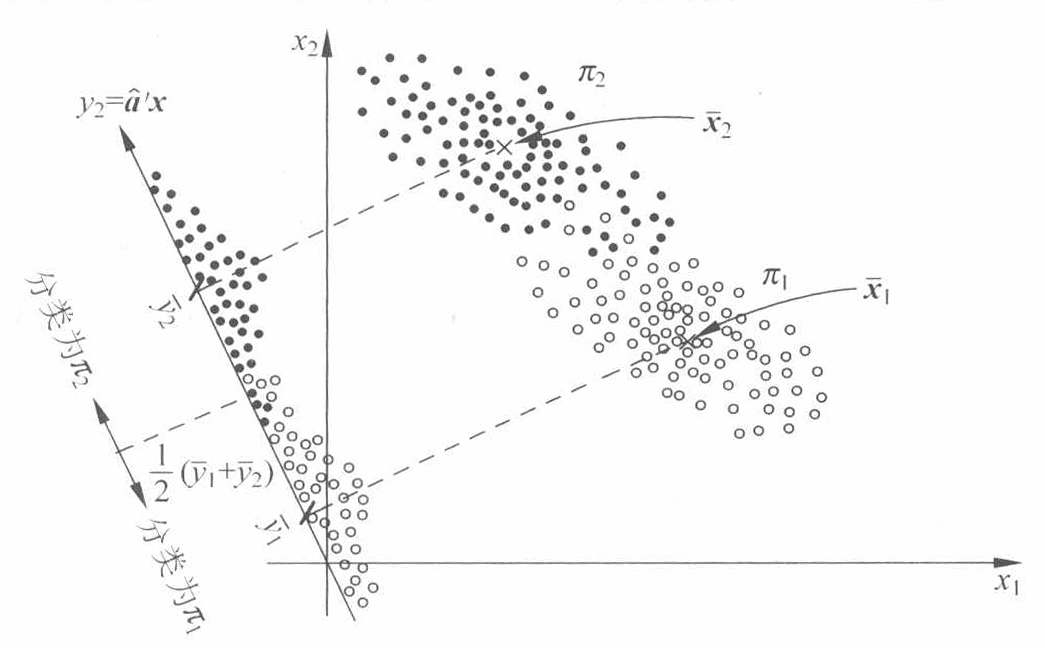
\includegraphics[width=88.5mm]{figs/fig_pg472_1.png}
\phantomsection\label{fig:11.5}\mvcap{图 11.5\quad 费希尔方法对两个总体的图形表示($p=2$)}
\end{mvfigure}

%% ===== pg-473 =====

% ---- pg-473 （书页 461） ----

费希尔的线性判别函数是在假定两个总体有相同协方差矩阵的条件下得到的. 因此毫不奇怪, 费希尔方法与最小期望错分代价法则这种特殊情况相对应. 分类法则(11-18)中的第一项 $\hat{y}=(\bar{\mathbf{x}}_1-\bar{\mathbf{x}}_2)'\mathbf{S}_{\mathrm{p}}^{-1}\mathbf{x}$ 就是费希尔的线性函数, 它使“组间变差”相对“组内变差”而言达到最大[见\hyperref[eq:11-23]{式(11-23)}]. 整个表达式
\phantomsection\label{eq:11-26}
\begin{equation}
\begin{aligned}
\hat{w}&=(\bar{\mathbf{x}}_1-\bar{\mathbf{x}}_2)'\mathbf{S}_{\mathrm{p}}^{-1}\mathbf{x}-\frac{1}{2}(\bar{\mathbf{x}}_1-\bar{\mathbf{x}}_2)'\mathbf{S}_{\mathrm{p}}^{-1}(\bar{\mathbf{x}}_1+\bar{\mathbf{x}}_2)\\
&=(\bar{\mathbf{x}}_1-\bar{\mathbf{x}}_2)'\mathbf{S}_{\mathrm{p}}^{-1}\left[\mathbf{x}-\frac{1}{2}(\bar{\mathbf{x}}_1+\bar{\mathbf{x}}_2)\right]
\end{aligned}
\tag{11-26}
\end{equation}
常被称为安德森(Anderson)分类函数(或称安德森统计量). 若 $[(c(1\mid2)/c(2\mid1))(p_2/p_1)]=1$, 则 $\ln[(c(1\mid2)/c(2\mid1))(p_2/p_1)]=0$, 法则(11-18)与基于费希尔线性判别函数的法则(11-26)相似. 这样, 费希尔分类法则等价于在相同先验概率和相同错分代价下的最小 ECM 法则.

\mvsub{分类是好的思想吗}

简而言之, 对两个总体, 通过考虑多元观测值的线性组合所得到的最大相对分离度等于距离 $D^2$. 这样就很方便, 因为在某些情况下, $D^2$ 可用于检验两个总体均值 $\boldsymbol{\mu}_1$ 和 $\boldsymbol{\mu}_2$ 是否有显著差异. 因此, 均值向量间有无差异的检验可看成是对所能达到的总体分离度的显著性检验.

假定总体 $\pi_1$ 和 $\pi_2$ 服从有相同协方差矩阵 $\boldsymbol{\Sigma}$ 的正态分布, 则如同在 6.3 节中那样, 对假设 $H_0:\boldsymbol{\mu}_1=\boldsymbol{\mu}_2$ 和 $H_1:\boldsymbol{\mu}_1\neq\boldsymbol{\mu}_2$ 的检验可用统计量
\[
\left(\frac{n_1+n_2-p-1}{(n_1+n_2-2)p}\right)\left(\frac{n_1n_2}{n_1+n_2}\right)D^2
\]
来完成, 这个统计量服从 $F$ 分布, 自由度为 $\nu_1=p$, $\nu_2=n_1+n_2-p-1$. 如果 $H_0$ 被拒绝, 我们可以认为 $\pi_1$ 与 $\pi_2$ 之间的分离度是显著的.

\noindent\mvbold{评注}\quad 显著分离并不一定意味良好的分类. 正如我们在 11.4 节中将会见到的, 可以对一个分类方法的有效性作出评估而不必依赖任何分离性检验. 另一方面, 如果分离不显著, 则寻找有用的分类法则将被证明是徒劳的.

\mvsub{当 \texorpdfstring{$\boldsymbol{\Sigma}_1\neq\boldsymbol{\Sigma}_2$}{Sigma1 != Sigma2} 时正态总体的分类}

如同所预料的那样, 当总体协方差矩阵不同时, 分类法则就更复杂.

考虑\hyperref[eq:11-10]{式(11-10)}中的多元正态密度, 并用 $\boldsymbol{\Sigma}_i$($i=1,2$)代替其中的 $\boldsymbol{\Sigma}$. 这样, 对两个总体来说, 不仅两个均值向量, 就是两个协方差矩阵也都不相同. 正如我们所见到, 最小 ECM 和最小 TPM 的区域依赖于密度比 $f_1(\mathbf{x})/f_2(\mathbf{x})$, 或等价地依赖于密度比的自然对数 $\ln[f_1(\mathbf{x})/f_2(\mathbf{x})]=\ln[f_1(\mathbf{x})]-\ln[f_2(\mathbf{x})]$. 当多元正态密度有不同的协方差结构时, 密度比中包含 $|\boldsymbol{\Sigma}_i|^{1/2}$ 的项就不会像 $\boldsymbol{\Sigma}_1=\boldsymbol{\Sigma}_2$ 时那样可以消掉. 此外, $f_1(\mathbf{x})$ 和 $f_2(\mathbf{x})$ 指数中的二次型也不能合并成如\hyperref[eq:11-13]{式(11-13)}中那样相当简单的结果.

将具有不同协方差矩阵的正态密度代入\hyperref[eq:11-6]{式(11-6)}, 取自然对数再化简(见练习 11.15), 得到分类域:
\phantomsection\label{eq:11-27}
\begin{equation}
\begin{aligned}
R_1:\ &-\frac{1}{2}\mathbf{x}'(\boldsymbol{\Sigma}_1^{-1}-\boldsymbol{\Sigma}_2^{-1})\mathbf{x}+(\boldsymbol{\mu}_1'\boldsymbol{\Sigma}_1^{-1}-\boldsymbol{\mu}_2'\boldsymbol{\Sigma}_2^{-1})\mathbf{x}-k\geqslant\ln\left[\left(\frac{c(1\mid2)}{c(2\mid1)}\right)\left(\frac{p_2}{p_1}\right)\right]\\
R_2:\ &-\frac{1}{2}\mathbf{x}'(\boldsymbol{\Sigma}_1^{-1}-\boldsymbol{\Sigma}_2^{-1})\mathbf{x}+(\boldsymbol{\mu}_1'\boldsymbol{\Sigma}_1^{-1}-\boldsymbol{\mu}_2'\boldsymbol{\Sigma}_2^{-1})\mathbf{x}-k<\ln\left[\left(\frac{c(1\mid2)}{c(2\mid1)}\right)\left(\frac{p_2}{p_1}\right)\right]
\end{aligned}
\tag{11-27}
\end{equation}
其中

%% ===== pg-474 =====

% ---- pg-474 （书页 462） ----

\phantomsection\label{eq:11-28}
\begin{equation}
k=\frac{1}{2}\ln\left(\frac{|\boldsymbol{\Sigma}_1|}{|\boldsymbol{\Sigma}_2|}\right)+\frac{1}{2}(\boldsymbol{\mu}_1'\boldsymbol{\Sigma}_1^{-1}\boldsymbol{\mu}_1-\boldsymbol{\mu}_2'\boldsymbol{\Sigma}_2^{-1}\boldsymbol{\mu}_2)
\tag{11-28}
\end{equation}
这些分类域由 $\mathbf{x}$ 的二次函数定义. 当 $\boldsymbol{\Sigma}_1=\boldsymbol{\Sigma}_2$ 时, 二次项 $-\frac{1}{2}\mathbf{x}'(\boldsymbol{\Sigma}_1^{-1}-\boldsymbol{\Sigma}_2^{-1})\mathbf{x}$ 消失, 于是由\hyperref[eq:11-27]{式(11-27)}所定义的区域退化为由\hyperref[eq:11-14]{式(11-14)}所定义的区域.

一般多元正态总体的分类法则直接由\hyperref[eq:11-27]{式(11-27)}得到.

\noindent\textbf{结论 11.4}\quad 设总体 $\pi_1$ 和 $\pi_2$ 由均值向量和协方差矩阵分别为 $\boldsymbol{\mu}_1$, $\boldsymbol{\Sigma}_1$ 和 $\boldsymbol{\mu}_2$, $\boldsymbol{\Sigma}_2$ 的正态密度所刻画, 则能使期望错分代价(ECM)达到最小的分配法则为:

当
\[
-\frac{1}{2}\mathbf{x}_0'(\boldsymbol{\Sigma}_1^{-1}-\boldsymbol{\Sigma}_2^{-1})\mathbf{x}_0+(\boldsymbol{\mu}_1'\boldsymbol{\Sigma}_1^{-1}-\boldsymbol{\mu}_2'\boldsymbol{\Sigma}_2^{-1})\mathbf{x}_0-k\geqslant\ln\left[\left(\frac{c(1\mid2)}{c(2\mid1)}\right)\left(\frac{p_2}{p_1}\right)\right]
\]
时将 $\mathbf{x}_0$ 分配给 $\pi_1$, 否则将 $\mathbf{x}_0$ 分配给 $\pi_2$.

这里 $k$ 由\hyperref[eq:11-28]{式(11-28)}所给出.

在实践中, 结论 11.4 中的分类法则是通过用样本量 $\bar{x}_1$, $\bar{x}_2$, $\mathbf{S}_1$ 和 $\mathbf{S}_2$[见\hyperref[eq:11-16]{式(11-16)}]分别代替总体量 $\boldsymbol{\mu}_1$, $\boldsymbol{\mu}_2$, $\boldsymbol{\Sigma}_1$ 和 $\boldsymbol{\Sigma}_2$ 来实施的.\footnote{为保证 $\mathbf{S}_1^{-1}$ 和 $\mathbf{S}_2^{-1}$ 存在, 不等式 $n_1>p$ 和 $n_2>p$ 都必须成立, 因为这样才能用 $\mathbf{S}_1^{-1}$ 和 $\mathbf{S}_2^{-1}$ 分别取代 $\boldsymbol{\Sigma}_1^{-1}$ 和 $\boldsymbol{\Sigma}_2^{-1}$, 从而得出样本分类法则(11-29).}

\begin{mvframe}[二次分类法则(有不同协方差阵的正态总体)]
若
\phantomsection\label{eq:11-29}
\begin{equation}
-\frac{1}{2}\mathbf{x}_0'(\mathbf{S}_1^{-1}-\mathbf{S}_2^{-1})\mathbf{x}_0+(\bar{\mathbf{x}}_1'\mathbf{S}_1^{-1}-\bar{\mathbf{x}}_2'\mathbf{S}_2^{-1})\mathbf{x}_0-k\geqslant\ln\left[\left(\frac{c(1\mid2)}{c(2\mid1)}\right)\left(\frac{p_2}{p_1}\right)\right]
\tag{11-29}
\end{equation}
则将 $\mathbf{x}_0$ 分配到 $\pi_1$, 否则将 $\mathbf{x}_0$ 分配到 $\pi_2$.
\end{mvframe}

在维数大于 2 的场合, 用二次函数进行分类相当困难, 而且会导致某些奇怪的结果. 尤其当数据(本质上)不服从正态分布时, 情况更是如此.

\hyperref[fig:11.6]{图 11.6}(a)显示了建立在具有两个不同方差的分布这一理想化情况基础上的相同代价及相同先验概率法则. 在这个场合, 这个二次分类法则导致区域 $R_1$ 由两个不相联结的集合组成.

在许多应用中, $\pi_1$ 分布的左尾部分比正态分布所描述的左尾部分要低. 于是正如同\hyperref[fig:11.6]{图 11.6}(b)所示的那样, 由二次法则产生的 $R_1$ 的左尾部分不能清晰地区分两个总体分布, 因此会导致较大的失误率. 二次法则的一个严重的弱点是对偏离正态性很敏感.

\begin{mvfigure}
\begin{tikzpicture}[xscale=0.75,yscale=1.05]
% ================= (a) =================
\begin{scope}
  \draw[->] (0,0) -- (6.7,0) node[below right]{$x$};
  \foreach \x in {0.06,0.12,...,6.42}{\draw (\x,0) -- (\x,-0.09);}
  \draw[domain=0.55:4.15,smooth,variable=\x] plot (\x,{1.35*exp(-((\x-2.3)*(\x-2.3))/(2*0.50*0.50))});
  \draw[domain=-0.25:6.65,smooth,variable=\x] plot (\x,{0.62*exp(-((\x-3.3)*(\x-3.3))/(2*1.55*1.55))});
  \node at (2.85,1.42) {$f_2(x)$};
  \node at (3.85,0.76) {$f_1(x)$};
  \draw[decorate,decoration={brace,amplitude=5pt,mirror}] (0.05,-0.28) -- (1.05,-0.28) node[midway,below=4pt]{$R_1$};
  \draw[decorate,decoration={brace,amplitude=5pt,mirror}] (1.35,-0.28) -- (3.40,-0.28) node[midway,below=4pt]{$R_2$};
  \draw[decorate,decoration={brace,amplitude=5pt,mirror}] (3.40,-0.28) -- (6.30,-0.28) node[midway,below=4pt]{$R_1$};
  \node at (3.35,-1.25) {(a)};
\end{scope}
% ================= (b) =================
\begin{scope}[xshift=8.3cm]
  \draw[->] (0,0) -- (6.7,0) node[below right]{$x$};
  \foreach \x in {0.06,0.12,...,6.42}{\draw (\x,0) -- (\x,-0.09);}
  \draw[domain=0.55:4.15,smooth,variable=\x] plot (\x,{1.35*exp(-((\x-2.3)*(\x-2.3))/(2*0.50*0.50))});
  \draw[domain=0.85:2.3,smooth,variable=\x] plot (\x,{0.60*exp(-((\x-2.3)*(\x-2.3))/(2*0.30*0.30))});
  \draw[domain=2.3:6.65,smooth,variable=\x] plot (\x,{0.60*exp(-((\x-2.3)*(\x-2.3))/(2*1.60*1.60))});
  \node at (2.80,1.42) {$f_2(x)$};
  \node at (3.65,0.76) {$f_1(x)$};
  \draw[decorate,decoration={brace,amplitude=5pt,mirror}] (0.05,-0.28) -- (0.95,-0.28) node[midway,below=4pt]{$R_1$};
  \draw[decorate,decoration={brace,amplitude=5pt,mirror}] (1.25,-0.28) -- (3.20,-0.28) node[midway,below=4pt]{$R_2$};
  \draw[decorate,decoration={brace,amplitude=5pt,mirror}] (3.20,-0.28) -- (6.40,-0.28) node[midway,below=4pt]{$R_1$};
  \node at (3.35,-1.25) {(b)};
\end{scope}
\end{tikzpicture}
\phantomsection\label{fig:11.6}\mvcap{图 11.6\quad 二次法则: (a) 两个方差不同的正态分布; (b) 两个分布, 其中一个为非正态分布——法则不适当}
\end{mvfigure}

%% ===== pg-475 =====

% ---- pg-475 （书页 463） ----

若数据为非多元正态数据, 则有两种可行的选择. 首先, 可将非正态性数据变换成接近正态性的数据, 然后进行协方差矩阵相等性的检验, 看看线性法则(11-18)和二次法则(11-29)哪个更合适. 可以考虑的变换在第 4 章中已有讨论. (通常的协方差齐次性检验受到非正态性的很大影响, 所以在进行这种检验之前必须将非正态性数据变换成正态性数据.)

其次, 可以使用线性(或二次)法则而不考虑母体分布的形式, 期望能产生相当好的效果. 但是对这个问题的研究表明, 在非正态情形下, 即使总体协方差矩阵相同, 线性分类函数的使用效果有时也非常差(见文献[22]和[23]). 由此得出结论: 一定要检查任何分类方法的效果. 至少必须对用于构造分类函数的数据作这种检查. 在理想的情况下, 会有足够的数据用作“训练”样本和“验证”样本. 训练样本用于构造分类函数, 而验证样本则用于评估分类的效果.

\section{评估分类函数}  % 原书 11.4
\phantomsection\label{sec:11.4}

判断任一分类方法效果的一个重要途径, 就是计算其“失误率”或错分概率. 当母总体分布形式完全已知时, 如例 11.5 所显示的那样, 错分概率的计算相对来说比较容易. 由于母总体分布很少是已知的, 我们将集中考虑与样本分类函数相联系的失误率. 一旦构造出一个分类函数, 我们就对如何度量它在未来样本中的性能感兴趣.

由\hyperref[eq:11-8]{式(11-8)}知, 总错分概率为
\[
\mathrm{TPM}=p_1\int_{R_2}f_1(\mathbf{x})\,\mathrm{d}\mathbf{x}+p_2\int_{R_1}f_2(\mathbf{x})\,\mathrm{d}\mathbf{x}
\]
通过适当选择 $R_1$ 和 $R_2$ 得出的该量的最小值, 称为最优失误率(OER).

\begin{mvframe}[最优失误率]
\phantomsection\label{eq:11-30}
\begin{equation}
\mathrm{OER}=p_1\int_{R_2}f_1(\mathbf{x})\,\mathrm{d}\mathbf{x}+p_2\int_{R_1}f_2(\mathbf{x})\,\mathrm{d}\mathbf{x}
\tag{11-30}
\end{equation}
其中 $R_1$ 和 $R_2$ 由\hyperref[eq:11-7]{式(11-7)}中的(b)所确定.
\end{mvframe}

这样, OER 就是最小 TPM 分类法则的失误率.

\noindent\textbf{例 11.5}\quad (计算错分概率)

让我们在 $p_1=p_2=1/2$, 并且\hyperref[eq:11-10]{式(11-10)}中的 $f_1(\mathbf{x})$ 和 $f_2(\mathbf{x})$ 为多元正态密度时导出最优失误率的表达式.

最小 ECM 分类法则和最小 TPM 分类法则在 $c(1\mid2)=c(2\mid1)$ 时彼此重合. 由于先验概率也相等, 所以最小 TPM 分类域对正态总体来说由\hyperref[eq:11-12]{式(11-12)}定义, 其中 $\ln\left[\left(\frac{c(1\mid2)}{c(2\mid1)}\right)\left(\frac{p_2}{p_1}\right)\right]=0$. 我们发现
\[
\begin{aligned}
R_1:\ &(\boldsymbol{\mu}_1-\boldsymbol{\mu}_2)'\boldsymbol{\Sigma}^{-1}\mathbf{x}-\frac{1}{2}(\boldsymbol{\mu}_1-\boldsymbol{\mu}_2)'\boldsymbol{\Sigma}^{-1}(\boldsymbol{\mu}_1+\boldsymbol{\mu}_2)\geqslant0\\
R_2:\ &(\boldsymbol{\mu}_1-\boldsymbol{\mu}_2)'\boldsymbol{\Sigma}^{-1}\mathbf{x}-\frac{1}{2}(\boldsymbol{\mu}_1-\boldsymbol{\mu}_2)'\boldsymbol{\Sigma}^{-1}(\boldsymbol{\mu}_1+\boldsymbol{\mu}_2)<0
\end{aligned}
\]
这些集合可用 $y=(\boldsymbol{\mu}_1-\boldsymbol{\mu}_2)'\boldsymbol{\Sigma}^{-1}\mathbf{x}=\mathbf{a}'\mathbf{x}$ 表示为
\[
\begin{aligned}
R_1(y):\ &y\geqslant\frac{1}{2}(\boldsymbol{\mu}_1-\boldsymbol{\mu}_2)'\boldsymbol{\Sigma}^{-1}(\boldsymbol{\mu}_1+\boldsymbol{\mu}_2)\\
R_2(y):\ &y<\frac{1}{2}(\boldsymbol{\mu}_1-\boldsymbol{\mu}_2)'\boldsymbol{\Sigma}^{-1}(\boldsymbol{\mu}_1+\boldsymbol{\mu}_2)
\end{aligned}
\]

%% ===== pg-476 =====

% ---- pg-476 （书页 464） ----

但 $Y$ 为正态随机变量的线性组合, 因此 $Y$ 的概率密度 $f_1(y)$ 和 $f_2(y)$ 服从一元正态分布(见结论 4.2), 其均值和方差分别为
\[
\begin{aligned}
\mu_{1Y}&=\mathbf{a}'\boldsymbol{\mu}_1=(\boldsymbol{\mu}_1-\boldsymbol{\mu}_2)'\boldsymbol{\Sigma}^{-1}\boldsymbol{\mu}_1\\
\mu_{2Y}&=\mathbf{a}'\boldsymbol{\mu}_2=(\boldsymbol{\mu}_1-\boldsymbol{\mu}_2)'\boldsymbol{\Sigma}^{-1}\boldsymbol{\mu}_2\\
\sigma_Y^2&=\mathbf{a}'\boldsymbol{\Sigma}\mathbf{a}=(\boldsymbol{\mu}_1-\boldsymbol{\mu}_2)'\boldsymbol{\Sigma}^{-1}(\boldsymbol{\mu}_1-\boldsymbol{\mu}_2)=\Delta^2
\end{aligned}
\]
现在,
\[
\mathrm{TPM}=\frac{1}{2}P(\text{将 }\pi_1\text{ 观测值错分入 }\pi_2)+\frac{1}{2}P(\text{将 }\pi_2\text{ 观测值错分入 }\pi_1)
\]
但是,
\[
\begin{aligned}
P[\text{将 }\pi_1\text{ 观测值错分入 }\pi_2]&=P(2\mid1)\\
&=P\left[Y<\frac{1}{2}(\boldsymbol{\mu}_1-\boldsymbol{\mu}_2)'\boldsymbol{\Sigma}^{-1}(\boldsymbol{\mu}_1+\boldsymbol{\mu}_2)\right]\\
&=P\left(\frac{Y-\mu_{1Y}}{\sigma_Y}<\frac{\frac{1}{2}(\boldsymbol{\mu}_1-\boldsymbol{\mu}_2)'\boldsymbol{\Sigma}^{-1}(\boldsymbol{\mu}_1+\boldsymbol{\mu}_2)-(\boldsymbol{\mu}_1-\boldsymbol{\mu}_2)'\boldsymbol{\Sigma}^{-1}\boldsymbol{\mu}_1}{\Delta}\right)\\
&=P\left(Z<-\frac{1}{2}\frac{\Delta^2}{\Delta}\right)=\Phi\left(-\frac{\Delta}{2}\right)
\end{aligned}
\]
其中 $\Phi(\cdot)$ 为标准正态分布的累积分布函数. 类似地,
\[
\begin{aligned}
P[\text{将 }\pi_2\text{ 观测值错分入 }\pi_1]&=P(1\mid2)=P\left[Y\geqslant\frac{1}{2}(\boldsymbol{\mu}_1-\boldsymbol{\mu}_2)'\boldsymbol{\Sigma}^{-1}(\boldsymbol{\mu}_1+\boldsymbol{\mu}_2)\right]\\
&=P\left(Z\geqslant\frac{\Delta}{2}\right)=1-\Phi\left(\frac{\Delta}{2}\right)=\Phi\left(-\frac{\Delta}{2}\right)
\end{aligned}
\]
这些错分概率示于\hyperref[fig:11.7]{图 11.7}. 最优失误率为
\phantomsection\label{eq:11-31}
\begin{equation}
\mathrm{OER}=\text{最小 TPM}=\frac{1}{2}\Phi\left(-\frac{\Delta}{2}\right)+\frac{1}{2}\Phi\left(-\frac{\Delta}{2}\right)=\Phi\left(-\frac{\Delta}{2}\right)
\tag{11-31}
\end{equation}
比方说, 若 $\Delta^2=(\boldsymbol{\mu}_1-\boldsymbol{\mu}_2)'\boldsymbol{\Sigma}^{-1}(\boldsymbol{\mu}_1-\boldsymbol{\mu}_2)=2.56$, 则 $\Delta=\sqrt{2.56}=1.6$. 利用附录中的表 1, 我们得到
\[
\text{最小 TPM}=\Phi\left(-\frac{1.6}{2}\right)=\Phi(-0.8)=0.211\,9
\]

\begin{mvfigure}
\begin{tikzpicture}[xscale=0.72,yscale=1.15]
  % 斜线阴影: f_1 在阈值左侧的面积 (P(2|1))
  \fill[pattern=north east lines,pattern color=black]
    (4.80,0) -- plot[domain=4.80:6.00,smooth,variable=\x]
      (\x,{exp(-((\x-8.0)*(\x-8.0))/(2*1.5*1.5))}) -- (6.00,0) -- cycle;
  % 点状阴影: f_2 在阈值右侧的面积 (P(1|2))
  \fill[pattern=dots,pattern color=black]
    (6.00,0) -- plot[domain=6.00:7.20,smooth,variable=\x]
      (\x,{exp(-((\x-4.0)*(\x-4.0))/(2*1.5*1.5))}) -- (7.20,0) -- cycle;
  \draw[domain=1.6:10.4,smooth,variable=\x] plot (\x,{exp(-((\x-4.0)*(\x-4.0))/(2*1.5*1.5))});
  \draw[domain=3.6:12.4,smooth,variable=\x] plot (\x,{exp(-((\x-8.0)*(\x-8.0))/(2*1.5*1.5))});
  \draw[->] (0,0) -- (13.2,0) node[below right]{$y$};
  \draw (6.00,0) -- (6.00,0.78);
  \node at (3.0,1.32) {$f_2(y)=N(\mu_{2Y},\ \Delta^2)$};
  \node at (10.6,1.32) {$f_1(y)=N(\mu_{1Y},\ \Delta^2)$};
  \node (p21) at (4.05,0.60) {$P(2\mid1)$};
  \draw (p21) -- (5.25,0.26);
  \node (p12) at (8.05,0.60) {$P(1\mid2)$};
  \draw (p12) -- (6.75,0.26);
  \draw[<->] (4.00,-0.30) -- (6.00,-0.30);
  \draw (4.00,-0.30) -- (4.00,-0.46);
  \draw (6.00,-0.30) -- (6.00,-0.46);
  \node[below] at (5.00,-0.46) {$\dfrac{\Delta^2}{2}$};
  \draw[<->] (6.00,-0.30) -- (8.00,-0.30);
  \draw (8.00,-0.30) -- (8.00,-0.46);
  \node[below] at (7.00,-0.46) {$\dfrac{\Delta^2}{2}$};
  \node[below] at (4.00,-0.70) {$\mu_{2Y}$};
  \node[below] at (8.60,-0.70) {$\mu_{1Y}$};
\end{tikzpicture}
\phantomsection\label{fig:11.7}\mvcap{图 11.7\quad 基于 $Y$ 的错分概率}
\end{mvfigure}

这个最优分类法则会错误地将大约 $21\%$ 的对象从一个总体分配到另一个总体.\hfill$\blacksquare$

例 11.5 说明当总体密度函数已知时, 如何计算最优失误率. 如果某些总体参数需要用样

%% ===== pg-477 =====

% ---- pg-477 （书页 465） ----

本来估计(通常情况就是如此), 那么失误率的计算就不那么直截了当了.

原则上, 样本分类函数的效果可以用真实失误率(AER)来评估:
\phantomsection\label{eq:11-32}
\begin{equation}
\mathrm{AER}=p_1\int_{\tilde{R}_2}f_1(\mathbf{x})\,\mathrm{d}\mathbf{x}+p_2\int_{\tilde{R}_1}f_2(\mathbf{x})\,\mathrm{d}\mathbf{x}
\tag{11-32}
\end{equation}
其中 $\tilde{R}_1$ 和 $\tilde{R}_2$ 表示由容量分别为 $n_1$ 和 $n_2$ 的样本所决定的分类域. 例如, 若使用\hyperref[eq:11-18]{式(11-18)}中的分类函数, 则区域 $\tilde{R}_1$ 和 $\tilde{R}_2$ 由满足下列不等式的 $\mathbf{x}$ 的集合来定义.
\[
\begin{aligned}
\tilde{R}_1:\ &(\bar{\mathbf{x}}_1-\bar{\mathbf{x}}_2)'\mathbf{S}_{\mathrm{p}}^{-1}\mathbf{x}-\frac{1}{2}(\bar{\mathbf{x}}_1-\bar{\mathbf{x}}_2)'\mathbf{S}_{\mathrm{p}}^{-1}(\bar{\mathbf{x}}_1+\bar{\mathbf{x}}_2)\geqslant\ln\left[\left(\frac{c(1\mid2)}{c(2\mid1)}\right)\left(\frac{p_2}{p_1}\right)\right]\\
\tilde{R}_2:\ &(\bar{\mathbf{x}}_1-\bar{\mathbf{x}}_2)'\mathbf{S}_{\mathrm{p}}^{-1}\mathbf{x}-\frac{1}{2}(\bar{\mathbf{x}}_1-\bar{\mathbf{x}}_2)'\mathbf{S}_{\mathrm{p}}^{-1}(\bar{\mathbf{x}}_1+\bar{\mathbf{x}}_2)<\ln\left[\left(\frac{c(1\mid2)}{c(2\mid1)}\right)\left(\frac{p_2}{p_1}\right)\right]
\end{aligned}
\]

AER 指出样本分类函数在未来样本中将如何表现. 同最优失误率一样, 一般来说 AER 不能计算, 因为它依赖于未知密度函数 $f_1(\mathbf{x})$ 和 $f_2(\mathbf{x})$. 但有一个与真实失误率有关的量的估计值却可以计算, 下面简短讨论一下.

存在一个分类方法效果的度量, 它不依赖于母体总体分布的形式, 并且对任意分类方法均可计算. 这个度量称为表观失误率(APER). 它定义为训练样本中被错分的观测值所占的比例.

表观失误率可以很容易地从模糊矩阵计算出来. 对来自 $\pi_1$ 的 $n_1$ 个观测值和来自 $\pi_2$ 的 $n_2$ 个观测值, 模糊矩阵的形式为

\phantomsection\label{eq:11-33}
\begin{equation}
\begin{array}{ll|cc|c}
 & & \multicolumn{2}{c|}{预测归属} & \\
 & & \pi_1 & \pi_2 & \\ \hline
\multirow{2}{*}{\makecell{真实\\归属}} & \pi_1 & n_{1C} & n_{1M}=n_1-n_{1C} & n_1\\
 & \pi_2 & n_{2M}=n_2-n_{2C} & n_{2C} & n_2
\end{array}
\tag{11-33}
\end{equation}

其中
\[
\begin{aligned}
n_{1C}&=\pi_1\text{ 中的对象被正确地分类为 }\pi_1\text{ 的个数}\\
n_{1M}&=\pi_1\text{ 中的对象被错误地分类为 }\pi_2\text{ 的个数}\\
n_{2C}&=\pi_2\text{ 中的对象被正确分类的个数}\\
n_{2M}&=\pi_2\text{ 中的对象被错误分类的个数}
\end{aligned}
\]
于是表观失误率为
\phantomsection\label{eq:11-34}
\begin{equation}
\mathrm{APER}=\frac{n_{1M}+n_{2M}}{n_1+n_2}
\tag{11-34}
\end{equation}
正好是训练样本中被错分的观测值所占的比例.

\noindent\textbf{例 11.6}\quad (计算表观失误率)

考虑\hyperref[fig:11.1]{图 11.1} 所示的机动割草机数据的分类域 $R_1$ 和 $R_2$. 这里, 实线右上方的数据被分类为 $\pi_1$, 即割草机拥有者; 实线左下方的数据被分类为 $\pi_2$. 注意, 某些观测值被错分了. 模糊矩阵为

\begin{mvtable}
\begin{tabular}{@{}ll|cc|c@{}}
\toprule
& & \multicolumn{2}{c|}{预测归属} & \\
& & $\pi_1$: 割草机拥有者 & $\pi_2$: 非拥有者 & \\
\midrule
\multirow{2}{*}{\makecell{实际\\归属}} & $\pi_1$: 拥有者 & $n_{1C}=10$ & $n_{1M}=2$ & $n_1=12$\\
 & $\pi_2$: 非拥有者 & $n_{2M}=2$ & $n_{2C}=10$ & $n_2=12$\\
\bottomrule
\end{tabular}
\end{mvtable}

%% ===== pg-478 =====

% ---- pg-478 （书页 466） ----

表观失误率为
\[
\mathrm{APER}=\left(\frac{2+2}{12+12}\right)\times100\%=\left(\frac{4}{24}\right)\times100\%=16.7\%
\]
\hfill$\blacksquare$

APER 具有直观上的感染力, 且易于计算. 不幸的是, 它倾向于低估 AER, 而且除非 $n_1$ 和 $n_2$ 非常大, 这个问题不会消失. 出现这种乐观估计的原因, 本质上由于是被用来构造分类函数的数据又被用于对这个函数进行评估.

可以构造比表观失误率更好的失误率估计值, 而且这种估计值相对来说也比较容易计算, 且不需要对分布做假定. 一种方法是将整个样本分成两部分: 训练样本和验证样本. 训练样本用于构造分类函数, 而验证样本则用于评估. 失误率用验证样本中被错分数据的比例来确定. 虽然这种方法不用同一组数据既构造又评估分类函数, 从而克服了偏倚问题, 但它有两个主要缺陷:

(i) 需要用大样本.

(ii) 所评估的函数并非感兴趣的函数. 这是因为最终几乎所有的数据都必须用于构造分类函数. 如果不是这样, 就会损失有价值的信息.

还有一种方法看起来效果较好, 称为拉亨布鲁克(Lachenbruch)的“提留”方法\footnote{此方法有时称为“刀切”, 或“交叉验证”.} (见文献[24]):

1. 从 $\pi_1$ 组观测值开始, 从这组数据中取出一个, 用其余 $n_1-1$ 个观测值和 $\pi_2$ 组的 $n_2$ 个观测值构造分类函数.

2. 用第 1 步中所构造的函数对“提留”的观测值进行分类.

3. 重复步骤 1 和 2, 直至 $\pi_1$ 中所有 $n_1$ 个观测值都被分类完毕为止. 令 $n_{1M}^{(H)}$ 为 $\pi_1$ 组中被错分的提留观测值个数.

4. 对 $\pi_2$ 中的观测值重复步骤 1 至 3. 令 $n_{2M}^{(H)}$ 为 $\pi_2$ 组中被错分的提留观测值个数.

在\hyperref[eq:11-1]{式(11-1)}和\hyperref[eq:11-2]{式(11-2)}中的条件错分概率 $P(2\mid1)$ 和 $P(1\mid2)$ 的估计量为:
\phantomsection\label{eq:11-35}
\begin{equation}
\begin{aligned}
\hat{P}(2\mid1)&=\frac{n_{1M}^{(H)}}{n_1}\\
\hat{P}(1\mid2)&=\frac{n_{2M}^{(H)}}{n_2}
\end{aligned}
\tag{11-35}
\end{equation}
总错分比例 $(n_{1M}^{(H)}+n_{2M}^{(H)})/(n_1+n_2)$ 为期望真实失误率 $E(\mathrm{AER})$ 的一个接近无偏的估计量, 即使对中等样本这个结论也对.

\begin{mvbox}
\phantomsection\label{eq:11-36}
\begin{equation}
\hat{E}(\mathrm{AER})=\frac{n_{1M}^{(H)}+n_{2M}^{(H)}}{n_1+n_2}
\tag{11-36}
\end{equation}
\end{mvbox}

拉亨布鲁克的提留方法与线性分类函数共同使用时, 计算上也是可行的. 在某些现有的判别分析的计算机程序中, 这种方法是所提供选择项目之一.

\noindent\textbf{例 11.7}\quad (用提留方法计算失误率的估计值)

我们将对\hyperref[eq:11-18]{式(11-18)}的相同代价和相同先验概率这种情况来说明拉亨布鲁克的提留方法和失误率估计值的计算. 考虑下列数据矩阵和描述性统计数字. (我们假定 $n_1=n_2=3$ 个二元观测值随机地取自两个总体 $\pi_1$ 和 $\pi_2$, 并假定它们有公共协方差阵.)

%% ===== pg-479 =====

% ---- pg-479 （书页 467） ----

\[
\mathbf{X}_1=\begin{bmatrix}2&12\\4&10\\3&8\end{bmatrix};\qquad \bar{\mathbf{x}}_1=\begin{bmatrix}3\\10\end{bmatrix},\quad 2\mathbf{S}_1=\begin{bmatrix}2&-2\\-2&8\end{bmatrix}
\]
\[
\mathbf{X}_2=\begin{bmatrix}5&7\\3&9\\4&5\end{bmatrix};\qquad \bar{\mathbf{x}}_2=\begin{bmatrix}4\\7\end{bmatrix},\quad 2\mathbf{S}_2=\begin{bmatrix}2&-2\\-2&8\end{bmatrix}
\]

联合协方差阵为
\[
\mathbf{S}_{\mathrm{p}}=\frac{1}{4}(2\mathbf{S}_1+2\mathbf{S}_2)=\begin{bmatrix}1&-1\\-1&4\end{bmatrix}
\]
利用 $\mathbf{S}_{\mathrm{p}}$, 其余数据以及\hyperref[eq:11-18]{式(11-18)}中同等代价同等先验概率的法则, 我们就可以对样本观测值进行分类. 然后可以验证(见练习 11.19), 模糊矩阵为
\[
\begin{array}{r|cc}
 & \multicolumn{2}{c}{\text{分类为:}}\\ \hline
\text{真实总体:} & \pi_1 & \pi_2\\ \hline
\pi_1 & 2 & 1\\
\pi_2 & 1 & 2
\end{array}
\]
因此,
\[
\mathrm{APER}(\text{表观失误率})=2/6=0.33
\]

从 $\mathbf{X}_1$ 中提留第一个观测值 $\mathbf{x}_H'=[2,12]$, 计算
\[
\mathbf{X}_{1H}=\begin{bmatrix}4&10\\3&8\end{bmatrix};\qquad \bar{\mathbf{x}}_{1H}=\begin{bmatrix}3.5\\9\end{bmatrix};\qquad 1\mathbf{S}_{1H}=\begin{bmatrix}0.5&1\\1&2\end{bmatrix}
\]
新的联合协方差阵 $\mathbf{S}_{H,\mathrm{p}}$ 为
\[
\mathbf{S}_{H,\mathrm{p}}=\frac{1}{3}[1\mathbf{S}_{1H}+2\mathbf{S}_2]=\frac{1}{3}\begin{bmatrix}2.5&-1\\-1&10\end{bmatrix}
\]
其逆\footnote{巴特利特(见文献[3])给出一个矩阵恒等式, 可用来直接从 $\mathbf{S}_{\mathrm{p}}^{-1}$ 迅速算出 $\mathbf{S}_{H,\mathrm{p}}^{-1}$. 这样就不需要在取出每个观测值后重新计算逆矩阵(见练习 11.20).}为
\[
\mathbf{S}_{H,\mathrm{p}}^{-1}=\frac{1}{8}\begin{bmatrix}10&1\\1&2.5\end{bmatrix}
\]
根据组均值 $\bar{\mathbf{x}}_{1H}$ 和 $\bar{\mathbf{x}}_2$ 之间的样本距离来分类提留观测值 $\bar{\mathbf{x}}_{1H}$, 计算起来更快一些. 这种方法等价于计算线性函数 $\hat{y}=\hat{\mathbf{a}}_{H}'\mathbf{x}_H=(\bar{\mathbf{x}}_{1H}-\bar{\mathbf{x}}_2)'\mathbf{S}_{H,\mathrm{p}}^{-1}\mathbf{x}_H$ 的值, 然后将它与中点 $\hat{m}_{H}=\frac{1}{2}(\bar{\mathbf{x}}_{1H}-\bar{\mathbf{x}}_2)'\mathbf{S}_{H,\mathrm{p}}^{-1}(\bar{\mathbf{x}}_{1H}+\bar{\mathbf{x}}_2)$ 作比较[见\hyperref[eq:11-19]{式(11-19)}和\hyperref[eq:11-20]{式(11-20)}].

这样, 对 $\mathbf{x}_H'=[2,12]$ 我们有

到 $\bar{\mathbf{x}}_{1H}$ 的平方距离 $=(\mathbf{x}_H-\bar{\mathbf{x}}_{1H})'\mathbf{S}_{H,\mathrm{p}}^{-1}(\mathbf{x}_H-\bar{\mathbf{x}}_{1H})$
\[
=[2-3.5\quad 12-9]\frac{1}{8}\begin{bmatrix}10&1\\1&2.5\end{bmatrix}\begin{bmatrix}2-3.5\\12-9\end{bmatrix}=4.5
\]
到 $\bar{\mathbf{x}}_2$ 的平方距离 $=(\mathbf{x}_H-\bar{\mathbf{x}}_2)'\mathbf{S}_{H,\mathrm{p}}^{-1}(\mathbf{x}_H-\bar{\mathbf{x}}_2)$

%% ===== pg-480 =====

% ---- pg-480 （书页 468） ----

\[
=[2-4\quad 12-7]\frac{1}{8}\begin{bmatrix}10&1\\1&2.5\end{bmatrix}\begin{bmatrix}2-4\\12-7\end{bmatrix}=10.3
\]

由于 $\mathbf{x}_H$ 到 $\bar{\mathbf{x}}_{1H}$ 的距离小于到 $\bar{\mathbf{x}}_2$ 的距离, 我们将 $\mathbf{x}_H$ 分类到 $\pi_1$. 在这种情形下, 分类是正确的.

如果提取 $\mathbf{x}_H'=[4,10]$, 则 $\bar{\mathbf{x}}_{1H}$ 和 $\mathbf{S}_{H,\mathrm{p}}^{-1}$ 变成
\[
\bar{\mathbf{x}}_{1H}=\begin{bmatrix}2.5\\10\end{bmatrix}\quad \text{和}\quad \mathbf{S}_{H,\mathrm{p}}^{-1}=\frac{1}{8}\begin{bmatrix}16&4\\4&2.5\end{bmatrix}
\]

我们发现
\[
\begin{aligned}
(\mathbf{x}_H-\bar{\mathbf{x}}_{1H})'\mathbf{S}_{H,\mathrm{p}}^{-1}(\mathbf{x}_H-\bar{\mathbf{x}}_{1H})&=[4-2.5\quad 10-10]\frac{1}{8}\begin{bmatrix}16&4\\4&2.5\end{bmatrix}\begin{bmatrix}4-2.5\\10-10\end{bmatrix}\\
&=4.5
\end{aligned}
\]
\[
\begin{aligned}
(\mathbf{x}_H-\bar{\mathbf{x}}_2)'\mathbf{S}_{H,\mathrm{p}}^{-1}(\mathbf{x}_H-\bar{\mathbf{x}}_2)&=[4-4\quad 10-7]\frac{1}{8}\begin{bmatrix}16&4\\4&2.5\end{bmatrix}\begin{bmatrix}4-4\\10-7\end{bmatrix}\\
&=2.8
\end{aligned}
\]

因此我们将错误地把 $\mathbf{x}_H'=[4,10]$ 指派给 $\pi_2$. 提取 $\mathbf{x}_H'=[3,8]$ 也会导致错误地将这个观测值指派给 $\pi_2$. 这样, $n_{1M}^{(H)}=2$.

转向第二组. 假定提取 $\mathbf{x}_H'=[5,7]$, 则
\[
\mathbf{X}_{2H}=\begin{bmatrix}3&9\\4&5\end{bmatrix};\quad \bar{\mathbf{x}}_{2H}=\begin{bmatrix}3.5\\7\end{bmatrix};\quad 1\mathbf{S}_{2H}=\begin{bmatrix}0.5&-2\\-2&8\end{bmatrix}
\]

新的联合协方差矩阵为
\[
\mathbf{S}_{H,\mathrm{p}}=\frac{1}{3}[2\mathbf{S}_1+1\mathbf{S}_{2H}]=\frac{1}{3}\begin{bmatrix}2.5&-4\\-4&16\end{bmatrix}
\]

其逆为
\[
\mathbf{S}_{H,\mathrm{p}}^{-1}=\frac{3}{24}\begin{bmatrix}16&4\\4&2.5\end{bmatrix}
\]

我们发现
\[
\begin{aligned}
(\mathbf{x}_H-\bar{\mathbf{x}}_1)'\mathbf{S}_{H,\mathrm{p}}^{-1}(\mathbf{x}_H-\bar{\mathbf{x}}_1)&=[5-3\quad 7-10]\frac{3}{24}\begin{bmatrix}16&4\\4&2.5\end{bmatrix}\begin{bmatrix}5-3\\7-10\end{bmatrix}\\
&=4.8
\end{aligned}
\]
\[
\begin{aligned}
(\mathbf{x}_H-\bar{\mathbf{x}}_{2H})'\mathbf{S}_{H,\mathrm{p}}^{-1}(\mathbf{x}_H-\bar{\mathbf{x}}_{2H})&=[5-3.5\quad 7-7]\frac{3}{24}\begin{bmatrix}16&4\\4&2.5\end{bmatrix}\begin{bmatrix}5-3.5\\7-7\end{bmatrix}\\
&=4.5
\end{aligned}
\]
因而 $\mathbf{x}_H'=[5,7]$ 被正确地指派给 $\pi_2$.

当 $\mathbf{x}_H'=[3,9]$ 被取出时,
\[
\begin{aligned}
(\mathbf{x}_H-\bar{\mathbf{x}}_1)'\mathbf{S}_{H,\mathrm{p}}^{-1}(\mathbf{x}_H-\bar{\mathbf{x}}_1)&=[3-3\quad 9-10]\frac{3}{24}\begin{bmatrix}10&1\\1&2.5\end{bmatrix}\begin{bmatrix}3-3\\9-10\end{bmatrix}\\
&=0.3
\end{aligned}
\]
\[
\begin{aligned}
(\mathbf{x}_H-\bar{\mathbf{x}}_{2H})'\mathbf{S}_{H,\mathrm{p}}^{-1}(\mathbf{x}_H-\bar{\mathbf{x}}_{2H})&=[3-4.5\quad 9-6]\frac{3}{24}\begin{bmatrix}10&1\\1&2.5\end{bmatrix}\begin{bmatrix}3-4.5\\9-6\end{bmatrix}\\
&=4.5
\end{aligned}
\]
于是 $\mathbf{x}_H'=[3,9]$ 被不正确地指派给 $\pi_1$. 最后, 提取 $\mathbf{x}_H'=[4,5]$ 导致将这个观测值正确地分到

%% ===== pg-481 =====

% ---- pg-481 （书页 469） ----

$\pi_2$. 这样, $n_{2M}^{(H)}=1$.

期望真实失误率的估计值为
\[
\hat{E}(\mathrm{AER})=\frac{n_{1M}^{(H)}+n_{2M}^{(H)}}{n_1+n_2}=\frac{2+1}{3+3}=0.5
\]
这样, 我们看到表观失误率 $\mathrm{APER}=0.33$ 是一个乐观的效果量度. 当然, 实践中的样本容量要比我们这里所考虑的容量大, 因而 $\mathrm{APER}$ 与 $\hat{E}(\mathrm{AER})$ 之间的差别没有本例中那么大. $\blacksquare$

有兴趣进一步了解分类失误率的估计方法的读者, 可参考文献[23].

下一个例子将说明当两个总体的判别方差不同时可能产生的一个困难.

\noindent\textbf{例 11.8}\quad (阿拉斯加产鲑鱼和加拿大产鲑鱼的分类)

捕捞鲑鱼对美国和加拿大两国来说都是一种有价值的资源. 由于这种资源有限, 因此必须有效地管理. 此外, 由于这个问题与两个国家有关, 必须公平地解决. 也就是说, 阿拉斯加的捕鱼者不能捕捞过多的加拿大产鲑鱼, 反之亦然.

这种鱼有一个奇怪的生命周期, 它们出生于淡水激流, 经过一到两年后游入大洋. 在海水中生活两年后, 它们又洄游到出生地, 产卵后死去. 在它们即将成熟, 在由大洋回游到淡水之前, 人们捕捞它们. 为了帮助规范捕捞, 在捕鱼季节, 管理人员从捕获的鱼中进行抽样检查, 以识别鱼是来自阿拉斯加还是来自加拿大产鲑鱼. 鱼鳞上的年轮可揭示产地. 典型的情况是: 阿拉斯加产鲑鱼的淡水生长年轮比加拿大产鲑鱼的要小. \hyperref[tab:11.2]{表 11.2} 给出了年轮的直径数据, 其中

\begin{align*}
X_1&=\text{第一年淡水生长的年轮直径(百分之一英寸)}\\
X_2&=\text{第一年海洋生长的年轮直径(百分之一英寸)}
\end{align*}

此外, 雌鱼取代码 1, 雄鱼则取代码 2.

\begin{mvtable}
\phantomsection\label{tab:11.2}\mvtabcap{表 11.2\quad 鲑鱼数据(年轮直径)}
\begin{tabular}{cccccc}
\toprule
\multicolumn{3}{c}{阿拉斯加} & \multicolumn{3}{c}{加拿大}\\
\cmidrule(lr){1-3}\cmidrule(lr){4-6}
性别 & 淡水 & 海洋 & 性别 & 淡水 & 海洋\\
\midrule
2 & 108 & 368 & 1 & 129 & 420\\
1 & 131 & 355 & 1 & 148 & 371\\
1 & 105 & 469 & 1 & 179 & 407\\
2 & 86 & 506 & 2 & 152 & 381\\
1 & 99 & 402 & 2 & 166 & 377\\
2 & 87 & 423 & 2 & 124 & 389\\
1 & 94 & 440 & 1 & 156 & 419\\
2 & 117 & 489 & 2 & 131 & 345\\
2 & 79 & 432 & 1 & 140 & 362\\
1 & 99 & 403 & 2 & 144 & 345\\
1 & 114 & 428 & 2 & 149 & 393\\
2 & 123 & 372 & 1 & 108 & 330\\
1 & 123 & 372 & 1 & 135 & 355\\
2 & 109 & 420 & 2 & 170 & 386\\
2 & 112 & 394 & 1 & 152 & 301\\
1 & 104 & 407 & 1 & 153 & 397\\
2 & 111 & 422 & 1 & 152 & 301\\
\bottomrule
\end{tabular}
\end{mvtable}

%% ===== pg-482 =====

% ---- pg-482 （书页 470） ----

\begin{mvtable}
\phantomsection\label{tab:11.2-2}\phantomsection\label{tab:11.2-2-2}\mvtabcap{表 11.2\quad 鲑鱼数据(年轮直径)(续表)}
\begin{longtable}{cccccc}\toprule
\multicolumn{3}{c}{阿拉斯加} & \multicolumn{3}{c}{加拿大}\\
\cmidrule(lr){1-3}\cmidrule(lr){4-6}
性别 & 淡水 & 海洋 & 性别 & 淡水 & 海洋\\
\midrule
\endfirsthead
\multicolumn{6}{c}{\zihao{6}续表}\\
\toprule
\multicolumn{3}{c}{阿拉斯加} & \multicolumn{3}{c}{加拿大}\\
\cmidrule(lr){1-3}\cmidrule(lr){4-6}
性别 & 淡水 & 海洋 & 性别 & 淡水 & 海洋\\
\midrule
\endhead
\bottomrule
\endlastfoot

2 & 126 & 423 & 2 & 136 & 438\\
2 & 105 & 434 & 2 & 122 & 306\\
1 & 119 & 474 & 1 & 148 & 383\\
1 & 114 & 396 & 2 & 90 & 385\\
2 & 100 & 470 & 1 & 145 & 337\\
2 & 84 & 399 & 1 & 123 & 364\\
2 & 102 & 429 & 2 & 145 & 376\\
2 & 101 & 469 & 2 & 115 & 354\\
2 & 85 & 444 & 2 & 134 & 383\\
1 & 109 & 397 & 1 & 117 & 355\\
2 & 106 & 442 & 2 & 126 & 345\\
1 & 82 & 431 & 1 & 118 & 379\\
2 & 118 & 381 & 2 & 120 & 369\\
1 & 105 & 388 & 1 & 153 & 403\\
1 & 121 & 403 & 2 & 150 & 354\\
1 & 85 & 451 & 1 & 154 & 390\\
1 & 83 & 453 & 1 & 155 & 349\\
1 & 53 & 427 & 2 & 109 & 325\\
1 & 95 & 411 & 2 & 117 & 344\\
1 & 76 & 442 & 1 & 128 & 400\\
1 & 95 & 426 & 1 & 144 & 403\\
2 & 87 & 402 & 2 & 163 & 370\\
1 & 70 & 397 & 2 & 145 & 355\\
2 & 84 & 511 & 1 & 133 & 375\\
2 & 91 & 469 & 1 & 128 & 383\\
1 & 74 & 451 & 2 & 123 & 349\\
2 & 101 & 474 & 1 & 144 & 373\\
1 & 80 & 398 & 2 & 140 & 388\\
1 & 95 & 433 & 2 & 150 & 339\\
2 & 92 & 404 & 2 & 124 & 341\\
1 & 99 & 481 & 1 & 125 & 346\\
2 & 94 & 491 & 1 & 153 & 352\\
1 & 87 & 480 & 1 & 108 & 339\\
\end{longtable}
\end{mvtable}

性别代码: $1=$雌性; $2=$雄性.

资料来源: 数据经阿拉斯加州渔业与捕猎部许可使用.

训练样本为 $n_1=50$ 条阿拉斯加产鲑鱼和 $n_2=50$ 条加拿大产鲑鱼. 由这些样本得出以下统计数字:
\[
\bar{\mathbf{x}}_1=\begin{bmatrix}98.380\\429.660\end{bmatrix},\qquad \mathbf{S}_1=\begin{bmatrix}260.608&-188.093\\-188.093&1\,399.086\end{bmatrix}
\]

%% ===== pg-483 =====

% ---- pg-483 （书页 471） ----

\[
\bar{\mathbf{x}}_2=\begin{bmatrix}137.460\\366.620\end{bmatrix},\qquad \mathbf{S}_2=\begin{bmatrix}326.090&133.505\\133.505&893.261\end{bmatrix}
\]

数据看上去满足二元正态分布的假定(见练习 11.31), 但协方差矩阵可能不同. 然而, 为说明与错分概率有关的要点, 我们仍采用线性判别方法.

使用同等代价和同等先验概率假定, 分类方法给出的提留估计失误率为

\begin{mvtable}
\begin{tabular}{ccc}
\toprule
& \multicolumn{2}{c}{预测归属}\\
\cmidrule(lr){2-3}
& $\pi_1$: 阿拉斯加 & $\pi_2$: 加拿大\\
\midrule
$\pi_1$: 阿拉斯加 & 44 & 6\\
$\pi_2$: 加拿大 & 1 & 49\\
\bottomrule
\end{tabular}
\end{mvtable}

其根据的线性判别函数[见\hyperref[eq:11-19]{式(11-19)}和\hyperref[eq:11-20]{式(11-20)}]为
\[
\hat{w}=\hat{y}-\bar{m}=-5.541\,21-0.128\,39x_1+0.051\,94x_2
\]
对两个总体, $\bar{w}$ 的样本标准差有所不同:

\begin{mvtable}
\begin{tabular}{cccc}
\toprule
& $n$ & \makecell{样本\\均值} & \makecell{样本\\标准差}\\
\midrule
阿拉斯加 & 50 & 4.144 & 3.253\\
加拿大 & 50 & $-4.147$ & 2.450\\
\bottomrule
\end{tabular}
\end{mvtable}

虽然总失误率(7\%)相当低, 但这里有一种不公平现象: 加拿大产的鲑鱼更不容易被错判为阿拉斯加产鲑鱼, 而不是相反. \hyperref[fig:11.8]{图 11.8} 显示线性判别函数 $\hat{y}$ 的两个正态密度. 由此图可以看出上面所说的现象. 采用两个样本均值的中点并未使两个错分概率相等. 显然, 具有较大方差的总体处于不利地位. 这样, 盲目地使用线性判别函数可能是不明智的. $\blacksquare$

\begin{mvfigure}
\begin{tikzpicture}[xscale=0.78,yscale=1.15]
\fill[pattern=north east lines,pattern color=black]
  (4.79,0) -- plot[domain=4.79:7.19,smooth,variable=\x] (\x,{1.13*exp(-((\x-9.67)*(\x-9.67))/(2*2.66*2.66))}) -- (7.19,0) -- cycle;
\draw[domain=0:11.9,smooth,variable=\x] plot (\x,{1.7*exp(-((\x-4.79)*(\x-4.79))/(2*1.85*1.85))});
\draw[domain=3.3:11.9,smooth,variable=\x] plot (\x,{1.13*exp(-((\x-9.67)*(\x-9.67))/(2*2.66*2.66))});
\draw[->] (0,0) -- (12.2,0) node[below right]{$y$};
\draw (7.19,0) -- (7.19,0.732);
\draw (4.79,0) -- (4.79,-0.07) node[below]{$\bar{y}_2$};
\draw (7.19,0) -- (7.19,-0.07) node[below]{$\hat{m}$};
\draw (9.67,0) -- (9.67,-0.07) node[below]{$\bar{y}_1$};
\end{tikzpicture}
\phantomsection\label{fig:11.8}\mvcap{图 11.8\quad 线性判别量的正态密度——鲑鱼数据}
\end{mvfigure}

直观上应该很清楚: 好的分类(低失误率)将依赖于总体的分离程度. 两个总体相互离得越远, 就越能得出有用的分类法则. 这个分离目标在 11.1 节中曾经提及, 我们在 11.6 节中将进一步探究.

正如我们将看到的, 在涉及相同先验概率和相同错分代价的场合, 分配法则与最大限度分离的总体的函数相对应. 正是在这种情形下, 分类与分离之间的界限开始消失.

\section{多个总体的分类}  % 原书 11.5
\phantomsection\label{sec:11.5}

理论上, 将两个总体的分类方法推广到 $g\ge 2$ 个总体是直截了当的. 不过我们对相应样本分类函数的性质所知不多, 特别是对它们的失误率尚未充分研究.

例如, 对两个总体的线性分类统计量, 其“稳健性”在不同协方差或非正态分布下可以用

%% ===== pg-484 =====

% ---- pg-484 （书页 472） ----

计算机生成的抽样实验来研究.\footnote{这里, 稳健性是指在执行某个分类方法时, 由于数据不满足方法所要求的假定而造成的失误率的恶化. 很难解析地研究分类方法的稳健性. 然而, 具有各式各样分布和不同协方差结构的数据很容易由计算机产生. 于是, 不同分类法则的效果可利用来自这些分布的由计算机生成的“样本”来评估.}但是对于多于两个总体的情况, 用这种方法不能得出一般结论, 因为统计量的性质依赖于总体的相互位置, 这里有太多的结构使得研究产生困难.

同前面一样, 本节的处置方法也是先从理论上导出一些最优法则, 然后指出将它们付诸实际应用时需要作哪些修正.

\subsection*{最小期望错分代价法}

设 $f_i(\mathbf{x})$ 为与总体 $\pi_i$ 相联系的密度, $i=1,2,\cdots,g$.[对本节的大部分内容, 我们将取 $f_i(\mathbf{x})$ 为多元正态密度, 但这在一般的理论推导中是不必要的.]令
\[
p_i=\text{总体 }\pi_i\text{ 的先验概率},\qquad i=1,2,\cdots,g
\]
\[
c(k\mid i)=\text{将事实上属于 }\pi_i\text{ 的某个项目分配到 }\pi_k\text{ 的代价},\qquad k,i=1,2,\cdots,g
\]
对 $k=i$, $c(i\mid i)=0$. 最后, 令 $R_k$ 为被分类为 $\pi_k$ 的 $\mathbf{x}$ 的集合, 因而对 $k,i=1,2,\cdots,g$ 有
\[
\begin{aligned}
P(k\mid i)&=P(\text{将项目分类为 }\pi_k\mid \pi_i)\\
&=\int_{R_k}f_i(\mathbf{x})\mathrm{d}\mathbf{x}
\end{aligned}
\]
且 $P(i\mid i)=1-\sum_{\substack{k=1\\k\ne i}}^{g}P(k\mid i)$.

将 $\pi_1$ 中的 $\mathbf{x}$ 错分到 $\pi_2$, 或 $\pi_3$, $\cdots$, 或 $\pi_g$ 的条件期望代价为
\[
\begin{aligned}
\mathrm{ECM}(1)&=P(2\mid 1)c(2\mid 1)+P(3\mid 1)c(3\mid 1)+\cdots+P(g\mid 1)c(g\mid 1)\\
&=\sum_{k=2}^{g}P(k\mid 1)c(k\mid 1)
\end{aligned}
\]
这个条件期望代价出现的先验概率为 $p_1$(即 $\pi_1$ 的概率).

用类似方法可得到条件期望错分代价 $\mathrm{ECM}(2),\cdots,\mathrm{ECM}(g)$. 对每个条件 ECM 乘以相应的先验概率再求和, 就得到总的 ECM:
\phantomsection\label{eq:11-37}
\begin{equation}
\begin{aligned}
\mathrm{ECM}&=p_1\mathrm{ECM}(1)+p_2\mathrm{ECM}(2)+\cdots+p_g\mathrm{ECM}(g)\\
&=p_1\left(\sum_{k=2}^{g}P(k\mid 1)c(k\mid 1)\right)+p_2\left(\sum_{\substack{k=1\\k\ne 2}}^{g}P(k\mid 2)c(k\mid 2)\right)\\
&\quad+\cdots+p_g\left(\sum_{k=1}^{g-1}P(k\mid g)c(k\mid g)\right)\\
&=\sum_{i=1}^{g}p_i\left(\sum_{\substack{k=1\\k\ne i}}^{g}P(k\mid i)c(k\mid i)\right)
\end{aligned}
\tag{11-37}
\end{equation}
确定一个最优分类法则相当于选择能使\hyperref[eq:11-37]{式(11-37)}达到极小的所有互斥区域 $R_1$, $R_2,\cdots,R_g$.

\noindent\textbf{结论 11.5}\quad 能使 ECM \hyperref[eq:11-37]{式(11-37)}达到极小的分类域, 可通过将 $\mathbf{x}$ 分配给使
\phantomsection\label{eq:11-38}
\begin{equation}
\sum_{\substack{i=1\\i\ne k}}^{g}p_if_i(\mathbf{x})c(k\mid i)
\tag{11-38}
\end{equation}
最小的总体 $\pi_k$($k=1,\cdots,g$)来定义. 当\hyperref[eq:11-38]{式(11-38)}最小的总体不止一个时, 则将 $\mathbf{x}$ 指派给其中

%% ===== pg-485 =====

% ---- pg-485 （书页 473） ----

的任一总体即可.

\noindent\mvbold{证明}\quad 见安德森(文献[2]).\hfill$\blacksquare$

假定所有错分代价都相等(不失一般性, 我们可令所有错分代价为 1), 则最小 ECM 法则就是最小总错分概率法则. 利用导出\hyperref[eq:11-38]{式(11-38)}的类似论据, 我们将 $\mathbf{x}$ 分配到 $\pi_k$, $k=1,2,\cdots,g$, 并使
\phantomsection\label{eq:11-39}
\begin{equation}
\sum_{\substack{i=1\\i\ne k}}^{g}p_if_i(\mathbf{x})
\tag{11-39}
\end{equation}
达到最小. 现在, 当被摒弃的项 $p_kf_k(\mathbf{x})$ 达到最大时, \hyperref[eq:11-39]{式(11-39)}将达到最小. 因此, 当错分代价相等时, 最小 ECM 法则具有下面的简单形式.

\begin{mvframe}[错分代价相同时的最小 ECM 分类法则]
若
\phantomsection\label{eq:11-40}
\begin{equation}
p_kf_k(\mathbf{x})>p_if_i(\mathbf{x}), \text{任意 } i\ne k
\tag{11-40}
\end{equation}
则将 $\mathbf{x}$ 分配到 $\pi_k$, 或等价的, 若
\phantomsection\label{eq:11-41}
\begin{equation}
\ln p_kf_k(\mathbf{x})>\ln p_if_i(\mathbf{x}), \text{任意 } i\ne k
\tag{11-41}
\end{equation}
则将 $\mathbf{x}$ 分配到 $\pi_k$.
\end{mvframe}

值得注意的是, 分类法则(11-40)等价于使“后验”概率 $P(\pi_k\mid \mathbf{x})=P$(给定观测值 $\mathbf{x}$, $\mathbf{x}$ 来自 $\pi_k$)最大化的法则, 其中
\phantomsection\label{eq:11-42}
\begin{equation}
P(\pi_k\mid \mathbf{x})=\frac{p_kf_k(\mathbf{x})}{\sum_{i=1}^{g}p_if_i(\mathbf{x})}=\frac{(\text{先验概率})\times(\text{密度函数})}{\sum(\text{先验概率})\times(\text{密度函数})}\qquad \text{对 } k=1,2,\cdots,g
\tag{11-42}
\end{equation}
\hyperref[eq:11-42]{式(11-42)}是\hyperref[eq:11-9]{式(11-9)}在 $g\ge 2$ 时的推广.

请记住, 一般来说, 最小 ECM 法则有三个要素: 先验概率、错分代价以及密度函数. 这些要素在使用分类法则之前必须指定(或估计出).

\noindent\textbf{例 11.9}\quad (将一个新观测值分到三个已知总体之一)

设虚构的先验概率、错分代价以及密度函数值给定如下表, 让我们将一个观测值 $\mathbf{x}_0$ 分到 $g=3$ 个总体 $\pi_1$, $\pi_2$ 和 $\pi_3$ 中的一个.

\begin{mvtable}
\begin{tabular}{l|cccc}
\toprule
& \multicolumn{4}{c}{真实总体}\\
\cmidrule(lr){2-5}
& & $\pi_1$ & $\pi_2$ & $\pi_3$\\
\midrule
\multirow{3}{*}{将 $\mathbf{x}_0$ 分到:} & $\pi_1$ & $c(1\mid 1)=0$ & $c(1\mid 2)=500$ & $c(1\mid 3)=100$\\
& $\pi_2$ & $c(2\mid 1)=10$ & $c(2\mid 2)=0$ & $c(2\mid 3)=50$\\
& $\pi_3$ & $c(3\mid 1)=50$ & $c(3\mid 2)=200$ & $c(3\mid 3)=0$\\
\midrule
先验概率: & & $p_1=0.05$ & $p_2=0.60$ & $p_3=0.35$\\
密度值: & & $f_1(\mathbf{x}_0)=0.01$ & $f_2(\mathbf{x}_0)=0.85$ & $f_3(\mathbf{x}_0)=2$\\
\bottomrule
\end{tabular}
\end{mvtable}

我们将采用最小 ECM 方法.

$\sum_{i=1}^{3}p_if_i(\mathbf{x}_0)c(k\mid i)$ 的值[见\hyperref[eq:11-38]{式(11-38)}]为

%% ===== pg-486 =====

% ---- pg-486 （书页 474） ----

\[
\begin{aligned}
k=1:\quad &p_2f_2(\mathbf{x}_0)c(1\mid 2)+p_3f_3(\mathbf{x}_0)c(1\mid 3)\\
&\quad=0.60\times 0.85\times 500+0.35\times 2\times 100=325\\
k=2:\quad &p_1f_1(\mathbf{x}_0)c(2\mid 1)+p_3f_3(\mathbf{x}_0)c(2\mid 3)\\
&\quad=0.05\times 0.01\times 10+0.35\times 2\times 50=35.055\\
k=3:\quad &p_1f_1(\mathbf{x}_0)c(3\mid 1)+p_2f_2(\mathbf{x}_0)c(3\mid 2)\\
&\quad=0.05\times 0.01\times 50+0.60\times 0.85\times 200=102.025
\end{aligned}
\]
由于 $k=2$ 时 $\sum_{\substack{i=1\\i\ne k}}^{3}p_if_i(\mathbf{x}_0)c(k\mid i)$ 最小, 我们将 $\mathbf{x}_0$ 分配到 $\pi_2$.

假定所有错分代价相等, 我们按\hyperref[eq:11-40]{式(11-40)}来分配 $\mathbf{x}_0$. 这只需计算下列乘积:
\[
\begin{aligned}
p_1f_1(\mathbf{x}_0)&=0.05\times 0.01=0.000\,5\\
p_2f_2(\mathbf{x}_0)&=0.60\times 0.85=0.510\\
p_3f_3(\mathbf{x}_0)&=0.35\times 2=0.700
\end{aligned}
\]
由于 $p_3f_3(\mathbf{x}_0)=0.700\ge p_if_i(\mathbf{x}_0)$, $i=1,2$, 我们将 $\mathbf{x}_0$ 分到 $\pi_3$. 等价的, 计算后验概率[见\hyperref[eq:11-42]{式(11-42)}], 得到
\[
P(\pi_1\mid \mathbf{x}_0)=\frac{p_1f_1(\mathbf{x}_0)}{\sum_{i=1}^{3}p_if_i(\mathbf{x}_0)}=\frac{0.05\times 0.01}{0.05\times 0.01+0.60\times 0.85+0.35\times 2}=\frac{0.000\,5}{1.210\,5}=0.000\,4
\]
\[
P(\pi_2\mid \mathbf{x}_0)=\frac{p_2f_2(\mathbf{x}_0)}{\sum_{i=1}^{3}p_if_i(\mathbf{x}_0)}=\frac{0.60\times 0.85}{1.210\,5}=\frac{0.510}{1.210\,5}=0.421
\]
\[
P(\pi_3\mid \mathbf{x}_0)=\frac{p_3f_3(\mathbf{x}_0)}{\sum_{i=1}^{3}p_if_i(\mathbf{x}_0)}=\frac{0.35\times 2}{1.210\,5}=\frac{0.700}{1.210\,5}=0.578
\]
我们看到, $\mathbf{x}_0$ 应分入具有最大后验概率的总体 $\pi_3$. \hfill$\blacksquare$

\subsection*{正态总体情形下的分类}

最重要的特例是当
\phantomsection\label{eq:11-43}
\begin{equation}
f_i(\mathbf{x})=\frac{1}{(2\pi)^{p/2}|\boldsymbol{\Sigma}_i|^{1/2}}\exp\left[-\frac{1}{2}(\mathbf{x}-\boldsymbol{\mu}_i)'\boldsymbol{\Sigma}_i^{-1}(\mathbf{x}-\boldsymbol{\mu}_i)\right],\qquad i=1,2,\cdots,g
\tag{11-43}
\end{equation}
为具有均值向量 $\boldsymbol{\mu}_i$ 和协方差矩阵 $\boldsymbol{\Sigma}_i$ 的正态密度函数的情形. 若进一步假定 $c(i\mid i)=0$, $c(k\mid i)=1$, $k\ne i$(或等价的, 所有错分代价相同), 则\hyperref[eq:11-41]{式(11-41)}变成:

若
\phantomsection\label{eq:11-44}
\begin{equation}
\begin{aligned}
\ln p_kf_k(\mathbf{x})&=\ln p_k-\left(\frac{p}{2}\right)\ln(2\pi)-\frac{1}{2}\ln|\boldsymbol{\Sigma}_k|-\frac{1}{2}(\mathbf{x}-\boldsymbol{\mu}_k)'\boldsymbol{\Sigma}_k^{-1}(\mathbf{x}-\boldsymbol{\mu}_k)\\
&=\max_i\ln p_if_i(\mathbf{x})
\end{aligned}
\tag{11-44}
\end{equation}
则将 $\mathbf{x}$ 分到 $\pi_k$.

在\hyperref[eq:11-44]{式(11-44)}中, 常数 $(p/2)\ln(2\pi)$ 可以略去, 因为它对所有总体都相同. 因此我们将第 $i$ 个总体的二次判别得分定义为
\phantomsection\label{eq:11-45}
\begin{equation}
d_i^Q(\mathbf{x})=-\frac{1}{2}\ln|\boldsymbol{\Sigma}_i|-\frac{1}{2}(\mathbf{x}-\boldsymbol{\mu}_i)'\boldsymbol{\Sigma}_i^{-1}(\mathbf{x}-\boldsymbol{\mu}_i)+\ln p_i,\qquad i=1,2,\cdots,g
\tag{11-45}
\end{equation}

%% ===== pg-487 =====

% ---- pg-487 （书页 475） ----

二次得分 $d_i^Q(\mathbf{x})$ 由广义方差 $|\boldsymbol{\Sigma}_i|$、先验概率 $p_i$ 和 $\mathbf{x}$ 到总体均值 $\boldsymbol{\mu}_i$ 的距离平方所组成. 不过注意, 对不同的总体, 必须使用不同的距离函数(等距离椭球的取向和大小均不同).

用这些判别得分我们发现, \hyperref[eq:11-44]{式(11-44)}中的分类法则可重新陈述如下:

\begin{mvframe}[正态总体和不同 $\boldsymbol{\Sigma}_i$ 情形下的最小总错分概率法则(TPM)]
若二次判别得分
\phantomsection\label{eq:11-46}
\begin{equation}
d_k^Q(\mathbf{x})=\max\{d_1^Q(\mathbf{x}), d_2^Q(\mathbf{x}), \cdots, d_g^Q(\mathbf{x})\}
\tag{11-46}
\end{equation}
则将 $\mathbf{x}$ 分入 $\pi_k$. 此处 $d_i^Q(\mathbf{x})$ 由\hyperref[eq:11-45]{式(11-45)}给出.
\end{mvframe}

实践中 $\boldsymbol{\mu}_i$ 和 $\boldsymbol{\Sigma}_i$ 皆属未知, 但常可获得一组已经正确分类的训练样本, 因此可以用样本均值 $\bar{\mathbf{x}}_i$ 来估计总体均值 $\boldsymbol{\mu}_i$, 以及用样本协方差矩阵 $\mathbf{S}_i$ 来估计总体协方差矩阵 $\boldsymbol{\Sigma}_i$. 此时二次判别得分 $d_i^Q(\mathbf{x})$ 的估计量为
\phantomsection\label{eq:11-47}
\begin{equation}
\hat{d}_i^Q(\mathbf{x})=-\frac{1}{2}\ln|\mathbf{S}_i|-\frac{1}{2}(\mathbf{x}-\bar{\mathbf{x}}_i)'\mathbf{S}_i^{-1}(\mathbf{x}-\bar{\mathbf{x}}_i)+\ln p_i,\qquad i=1,2,\cdots,g
\tag{11-47}
\end{equation}
于是基于样本的分类法则如下:

\begin{mvframe}[估计的最小 TPM 法则(对 $\boldsymbol{\Sigma}_i$ 不同的多个正态总体)]
若二次判别得分
\phantomsection\label{eq:11-48}
\begin{equation}
\hat{d}_k^Q(\mathbf{x})=\max\{\hat{d}_1^Q(\mathbf{x}), \hat{d}_2^Q(\mathbf{x}), \cdots, \hat{d}_g^Q(\mathbf{x})\}
\tag{11-48}
\end{equation}
则将 $\mathbf{x}$ 分入 $\pi_k$, 此处 $\hat{d}_i^Q(\mathbf{x})$ 由\hyperref[eq:11-47]{式(11-47)}给出.
\end{mvframe}

如果总体协方差矩阵相同, 上述判别法则有可能简化. 当 $\boldsymbol{\Sigma}_i=\boldsymbol{\Sigma}$, $i=1,2,\cdots,g$, \hyperref[eq:11-45]{式(11-45)}中的判别得分变成
\[
d_i^Q(\mathbf{x})=-\frac{1}{2}\ln|\boldsymbol{\Sigma}|-\frac{1}{2}\mathbf{x}'\boldsymbol{\Sigma}^{-1}\mathbf{x}+\boldsymbol{\mu}_i'\boldsymbol{\Sigma}^{-1}\mathbf{x}-\frac{1}{2}\boldsymbol{\mu}_i'\boldsymbol{\Sigma}^{-1}\boldsymbol{\mu}_i+\ln p_i
\]
此式右端的前两项对所有 $d_1^Q(\mathbf{x}),\cdots,d_g^Q(\mathbf{x})$ 都相同, 对分配目的来说可以略去. 剩余诸项由常数项 $c_i=\ln p_i-\frac{1}{2}\boldsymbol{\mu}_i'\boldsymbol{\Sigma}^{-1}\boldsymbol{\mu}_i$ 和 $\mathbf{x}$ 诸分量的一个线性组合组成.

下一步, 定义线性判别得分
\phantomsection\label{eq:11-49}
\begin{equation}
d_i(\mathbf{x})=\boldsymbol{\mu}_i'\boldsymbol{\Sigma}^{-1}\mathbf{x}-\frac{1}{2}\boldsymbol{\mu}_i'\boldsymbol{\Sigma}^{-1}\boldsymbol{\mu}_i+\ln p_i,\qquad i=1,2,\cdots,g
\tag{11-49}
\end{equation}
根据 $\boldsymbol{\Sigma}$ 的联合估计量
\phantomsection\label{eq:11-50}
\begin{equation}
\mathbf{S}_{\mathrm{p}}=\frac{1}{n_1+n_2+\cdots+n_g-g}((n_1-1)\mathbf{S}_1+(n_2-1)\mathbf{S}_2+\cdots+(n_g-1)\mathbf{S}_g)
\tag{11-50}
\end{equation}
可得到线性得分 $d_i(\mathbf{x})$ 的估计量
\phantomsection\label{eq:11-51}
\begin{equation}
\hat{d}_i(\mathbf{x})=\mathbf{x}'\mathbf{S}_{\mathrm{p}}^{-1}\bar{\mathbf{x}}_i-\frac{1}{2}\bar{\mathbf{x}}_i'\mathbf{S}_{\mathrm{p}}^{-1}\bar{\mathbf{x}}_i+\ln p_i,\qquad i=1,2,\cdots,g
\tag{11-51}
\end{equation}
因此我们有如下法则:

\begin{mvframe}[估计的最小 TPM 法则(对协方差矩阵相同的正态总体)]
若线性判别得分
\phantomsection\label{eq:11-52}
\begin{equation}
\hat{d}_k(\mathbf{x})=\max\{\hat{d}_1(\mathbf{x}), \hat{d}_2(\mathbf{x}), \cdots, \hat{d}_g(\mathbf{x})\}
\tag{11-52}
\end{equation}
则将 $\mathbf{x}$ 分入 $\pi_k$, 此处 $\hat{d}_i(\mathbf{x})$ 由\hyperref[eq:11-51]{式(11-51)}给出.
\end{mvframe}

%% ===== pg-488 =====

% ---- pg-488 （书页 476） ----

\noindent\textbf{评注}\quad \hyperref[eq:11-49]{式(11-49)}为 $\mathbf{x}$ 的一个简单的线性函数. 对协方差矩阵相同的情形, 在\hyperref[eq:11-45]{式(11-45)}中略去常数项 $-\frac{1}{2}\ln|\boldsymbol{\Sigma}|$, 便可得出一个等价的分类函数. 将未知总体参数用样本的估计量代替, 就可用 $\mathbf{x}$ 到样本均值向量 $\bar{\mathbf{x}}_i$ 的平方距离
\phantomsection\label{eq:11-53}
\begin{equation}
D_i^2(\mathbf{x})=(\mathbf{x}-\bar{\mathbf{x}}_i)'\mathbf{S}_{\mathrm{p}}^{-1}(\mathbf{x}-\bar{\mathbf{x}}_i)
\tag{11-53}
\end{equation}
来解释上述结果. 于是分配法则为:
\phantomsection\label{eq:11-54}
\begin{equation}
\text{若 }-\frac{1}{2}D_i^2(\mathbf{x})+\ln p_i\text{ 最大, 则将 }\mathbf{x}\text{ 分到总体 }\pi_i
\tag{11-54}
\end{equation}
我们看到, 这个法则将 $\mathbf{x}$ 分到“最近”的总体(距离量度受到 $\ln p_i$ 的干扰).

若先验概率未知, 通常的做法是令 $p_1=p_2=\cdots=p_g=1/g$. 这时观测值被分入最近的总体.

\noindent\textbf{例 11.10}\quad (在假定有公共协方差阵的条件下计算样本判别得分)

让我们在 $g=3$ 个总体, 有相同协方差矩阵的二元正态分布下来计算线性判别得分. 来自总体 $\pi_1$, $\pi_2$ 和 $\pi_3$ 的随机样本、均值向量和样本协方差阵为:
\[
\pi_1:\mathbf{X}_1=\begin{bmatrix}-2&5\\0&3\\-1&1\end{bmatrix},\quad n_1=3,\quad \bar{\mathbf{x}}_1=\begin{bmatrix}-1\\3\end{bmatrix},\quad \mathbf{S}_1=\begin{bmatrix}1&-1\\-1&4\end{bmatrix}
\]
\[
\pi_2:\mathbf{X}_2=\begin{bmatrix}0&6\\2&4\\1&2\end{bmatrix},\quad n_2=3,\quad \bar{\mathbf{x}}_2=\begin{bmatrix}1\\4\end{bmatrix},\quad \mathbf{S}_2=\begin{bmatrix}1&-1\\-1&4\end{bmatrix}
\]
\[
\pi_3:\mathbf{X}_3=\begin{bmatrix}1&-2\\0&0\\-1&4\end{bmatrix},\quad n_3=3,\quad \bar{\mathbf{x}}_3=\begin{bmatrix}0\\-2\end{bmatrix},\quad \mathbf{S}_3=\begin{bmatrix}1&1\\1&4\end{bmatrix}
\]
给定 $p_1=p_2=0.25$, $p_3=0.50$, 我们来根据\hyperref[eq:11-52]{式(11-52)}将 $\mathbf{x}_0'=[x_{01},x_{02}]=[-2,-1]$ 进行分类. 由\hyperref[eq:11-50]{式(11-50)},
\[
\begin{aligned}
\mathbf{S}_{\mathrm{p}}&=\frac{3-1}{9-3}\begin{bmatrix}1&-1\\-1&4\end{bmatrix}+\frac{3-1}{9-3}\begin{bmatrix}1&-1\\-1&4\end{bmatrix}+\frac{3-1}{9-3}\begin{bmatrix}1&1\\1&4\end{bmatrix}\\
&=\frac{2}{6}\begin{bmatrix}1+1+1&-1-1+1\\-1-1+1&4+4+4\end{bmatrix}=\begin{bmatrix}1&-\frac{1}{3}\\-\frac{1}{3}&4\end{bmatrix}
\end{aligned}
\]
故
\[
\mathbf{S}_{\mathrm{p}}^{-1}=\frac{9}{35}\begin{bmatrix}4&\frac{1}{3}\\[2pt]\frac{1}{3}&1\end{bmatrix}=\frac{1}{35}\begin{bmatrix}36&3\\3&9\end{bmatrix}
\]
其次有
\[
\bar{\mathbf{x}}_1'\mathbf{S}_{\mathrm{p}}^{-1}=[-1\quad 3]\frac{1}{35}\begin{bmatrix}36&3\\3&9\end{bmatrix}=\frac{1}{35}[-27\quad 24]
\]
因而
\[
\bar{\mathbf{x}}_1'\mathbf{S}_{\mathrm{p}}^{-1}\bar{\mathbf{x}}_1=\frac{1}{35}[-27\quad 24]\begin{bmatrix}-1\\3\end{bmatrix}=\frac{99}{35}
\]

%% ===== pg-489 =====

% ---- pg-489 （书页 477） ----

故
\[
\begin{aligned}
\hat{d}_1(\mathbf{x}_0)&=\ln p_1+\bar{\mathbf{x}}_1'\mathbf{S}_{\mathrm{p}}^{-1}\mathbf{x}_0-\frac{1}{2}\bar{\mathbf{x}}_1'\mathbf{S}_{\mathrm{p}}^{-1}\bar{\mathbf{x}}_1\\
&=\ln(0.25)+\left(\frac{-27}{35}\right)x_{01}+\left(\frac{24}{35}\right)x_{02}-\frac{1}{2}\times\frac{99}{35}
\end{aligned}
\]
注意 $\hat{d}_1(\mathbf{x}_0)=$ 常数 $+$ 常数 $\cdot\,x_{01}+$ 常数 $\cdot\,x_{02}$ 这一关系的线性形式. 用类似方法得到
\[
\bar{\mathbf{x}}_2'\mathbf{S}_{\mathrm{p}}^{-1}=[1\quad 4]\frac{1}{35}\begin{bmatrix}36&3\\3&9\end{bmatrix}=\frac{1}{35}[48\quad 39]
\]
\[
\bar{\mathbf{x}}_2'\mathbf{S}_{\mathrm{p}}^{-1}\bar{\mathbf{x}}_2=\frac{1}{35}[48\quad 39]\begin{bmatrix}1\\4\end{bmatrix}=\frac{204}{35}
\]
因而
\[
\hat{d}_2(\mathbf{x}_0)=\ln(0.25)+\left(\frac{48}{35}\right)x_{01}+\left(\frac{39}{35}\right)x_{02}-\frac{1}{2}\times\frac{204}{35}
\]
最后,
\[
\bar{\mathbf{x}}_3'\mathbf{S}_{\mathrm{p}}^{-1}=[0\quad -2]\frac{1}{35}\begin{bmatrix}36&3\\3&9\end{bmatrix}=\frac{1}{35}[-6\quad -18]
\]
\[
\bar{\mathbf{x}}_3'\mathbf{S}_{\mathrm{p}}^{-1}\bar{\mathbf{x}}_3=\frac{1}{35}[-6\quad -18]\begin{bmatrix}0\\-2\end{bmatrix}=\frac{36}{35}
\]
以及
\[
\hat{d}_3(\mathbf{x}_0)=\ln(0.50)+\left(\frac{-6}{35}\right)x_{01}+\left(\frac{-18}{35}\right)x_{02}-\frac{1}{2}\times\frac{36}{35}
\]
将数值 $x_{01}=-2$ 和 $x_{02}=-1$ 代入, 得到
\[
\hat{d}_1(\mathbf{x}_0)=-1.386+\left(\frac{-27}{35}\right)\times(-2)+\left(\frac{24}{35}\right)\times(-1)-\frac{99}{70}=-1.943
\]
\[
\hat{d}_2(\mathbf{x}_0)=-1.386+\left(\frac{48}{35}\right)\times(-2)+\left(\frac{39}{35}\right)\times(-1)-\frac{204}{70}=-8.158
\]
\[
\hat{d}_3(\mathbf{x}_0)=-0.693+\left(\frac{-6}{35}\right)\times(-2)+\left(\frac{-18}{35}\right)\times(-1)-\frac{36}{70}=-0.350
\]
由于 $\hat{d}_3(\mathbf{x}_0)=-0.350$ 为最大判别得分, 我们将 $\mathbf{x}_0$ 分入 $\pi_3$. \hfill$\blacksquare$

\noindent\textbf{例 11.11}\quad (对一个潜在的商学院研究生分类)

一所商学院的招生人员将本科生的平均毕业成绩(GPA)和本科毕业生的管理能力测验(GMAT)成绩用作“指标”, 帮助他决定应将哪些申报者接收为学院研究生. \hyperref[fig:11.9]{图 11.9} 显示了三组近期报名者的 $x_1=$GPA 和 $x_2=$GMAT 成绩. 这三个组是: $\pi_1$: 接收; $\pi_2$: 不接收; $\pi_3$: 处于接收与不接收的边缘.\footnote{本例中的总体都是虚构的. 另一方面, 经验表明, GPA 和 GMAT 得分高的学生一般能很好完成研究生学业, 而那些得分低的学生则会遇到困难.}

\hyperref[fig:11.9]{图 11.9} 中各点的数据列于\hyperref[tab:11.6]{表 11.6}(见练习 11.29). 这些数据产生下面的量(见显示板 11.1 中的 SAS 统计软件输出):

%% ===== pg-490 =====

% ---- pg-490 （书页 478） ----

\begin{mvfigure}
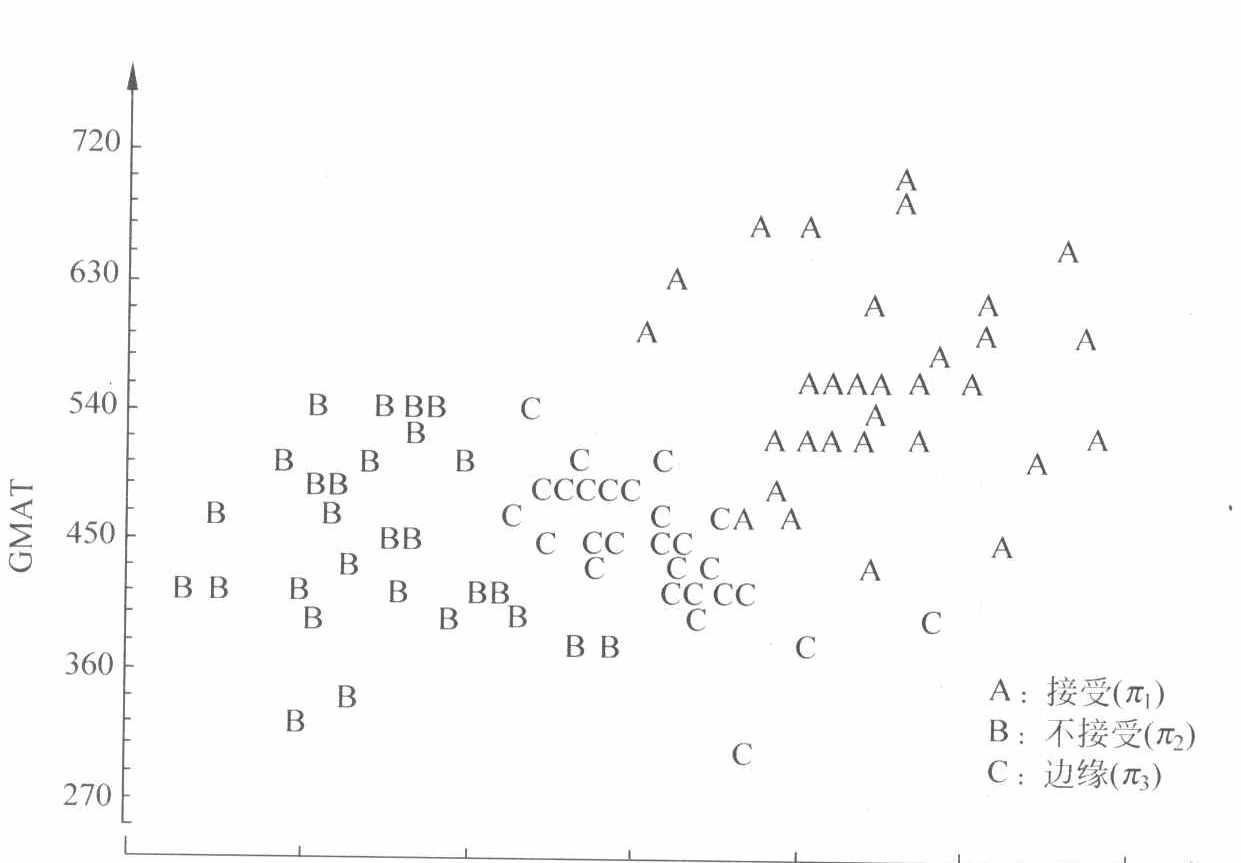
\includegraphics[width=105.0mm]{figs/fig_pg490_1.png}
\phantomsection\label{fig:11.9}\mvcap{图 11.9\quad 商学院研究生院申请者的散布图($x_1=$GPA, $x_2=$GMAT)}
\end{mvfigure}

\[
\begin{array}{ccc}
n_1=31 & n_2=28 & n_3=26\\[6pt]
\bar{\mathbf{x}}_1=\begin{bmatrix}3.40\\561.23\end{bmatrix} &
\bar{\mathbf{x}}_2=\begin{bmatrix}2.48\\447.07\end{bmatrix} &
\bar{\mathbf{x}}_3=\begin{bmatrix}2.99\\446.23\end{bmatrix}
\end{array}
\]
\[
\bar{\mathbf{x}}=\begin{bmatrix}2.97\\488.45\end{bmatrix},\qquad
\mathbf{S}_{\mathrm{p}}=\begin{bmatrix}0.036\,1&-2.018\,8\\-2.018\,8&3\,655.901\,1\end{bmatrix}
\]

假定一名新申请者的 GPA 成绩 $x_1=3.21$ 和 GMAT 成绩 $x_2=497$. 让我们用先验概率相等条件下的法则(11-54)对这名申请者进行分类.

因为 $\mathbf{x}_0'=[3.21,497]'$, 样本距离为
\[
\begin{aligned}
D_1^2(\mathbf{x}_0)&=(\mathbf{x}_0-\bar{\mathbf{x}}_1)'\mathbf{S}_{\mathrm{p}}^{-1}(\mathbf{x}_0-\bar{\mathbf{x}}_1)\\
&=[3.21-3.40,\ 497-561.23]\begin{bmatrix}28.609\,6&0.015\,8\\0.015\,8&0.000\,3\end{bmatrix}\begin{bmatrix}3.21-3.40\\497-561.23\end{bmatrix}\\
&=2.58
\end{aligned}
\]
\[
D_2^2(\mathbf{x}_0)=(\mathbf{x}_0-\bar{\mathbf{x}}_2)'\mathbf{S}_{\mathrm{p}}^{-1}(\mathbf{x}_0-\bar{\mathbf{x}}_2)=17.10
\]
\[
D_3^2(\mathbf{x}_0)=(\mathbf{x}_0-\bar{\mathbf{x}}_3)'\mathbf{S}_{\mathrm{p}}^{-1}(\mathbf{x}_0-\bar{\mathbf{x}}_3)=2.47
\]
因为从 $\mathbf{x}_0'=[3.21,497]$ 到组平均值 $\bar{\mathbf{x}}_3$ 的距离 $D_3(\mathbf{x}_0)$ 最小, 我们将这名申请者分入边缘总体 $\pi_3$. \hfill$\blacksquare$

\noindent\textbf{显示板 11.1}\quad 使用 SAS 的判别程序(PROC DISCRIM)对录取数据所作的分析

\begin{mvframe}
\begin{tabular}{@{}p{0.62\linewidth}@{\hspace{1em}}p{0.3\linewidth}@{}}
{\ttfamily title 'Discriminant Analysis';\newline
data gpa;\newline
infile 'T11-6.dat';\newline
input gpa gmat admit \$;\newline
proc discrim data = gpa\newline
method = normal pool = yes manova wcov pcov listerr crosslisterr;\newline
priors 'admit' = .333\,3 'notadmit' = .333\,3 'border' = .333\,3;\newline
class admit; var gpa gmat;}
& \raisebox{-1.4em}{\Huge\}} \mvbold{PROGRAM COMMANDS}
\end{tabular}
\end{mvframe}

%% ===== pg-491 =====

% ---- pg-491 （书页 479） ----

显示板 11.1(续)

\begin{mvbox}
{\ttfamily\small
\begin{center}
\begin{tabular}{@{}lll@{}}
\multicolumn{3}{c}{DISCRIMINANT ANALYSIS}\\
85 Observations & 84 DF Total & \multirow{3}{*}{\textbf{OUTPUT}}\\
2 Variables & 82 DF Within Classes\\
3 Classes & 2 DF Between Classes\\[4pt]
\multicolumn{3}{c}{Class Level Information}\\[4pt]
\end{tabular}
\end{center}

\begin{center}
\begin{tabular}{|l|r|r|r|r|}
\hline
ADMIT & Frequency & Weight & Proportion & Prior Probability\\
\hline
admit & 31 & 31.000\,0 & 0.364\,706 & 0.333\,333\\
border & 26 & 26.000\,0 & 0.305\,882 & 0.333\,333\\
notadmit & 28 & 28.000\,0 & 0.329\,412 & 0.333\,333\\
\hline
\end{tabular}
\end{center}

\begin{center}
\begin{tabular}{@{}lll@{}}
\multicolumn{3}{c}{DISCRIMINANT ANALYSIS\quad WITHIN-CLASS COVARIANCE MATRICES}\\
\multicolumn{3}{c}{ADMIT = admit\qquad DF = 30}\\
Variable & GPA & GMAT\\
GPA & 0.043\,558 & 0.058\,097\\
GMAT & 0.058\,097 & 4\,618.247\,312\\ \hdashline
\multicolumn{3}{c}{ADMIT = border\qquad DF = 25}\\
Variable & GPA & GMAT\\
GPA & 0.029\,692 & $-5.403\,846$\\
GMAT & $-5.403\,846$ & 2\,246.904\,615\\ \hdashline
\multicolumn{3}{c}{ADMIT = notadmit\qquad DF = 27}\\
Variable & GPA & GMAT\\
GPA & 0.033\,649 & $-1.192\,037$\\
GMAT & $-1.192\,037$ & 3\,891.253\,968\\
\end{tabular}
\end{center}

\begin{center}
\begin{tabular}{|l|l|@{}}
\hline
Pooled Within-Class Covariance Matrix & DF = 82\\
\hline
\end{tabular}
\end{center}

\begin{center}
\begin{tabular}{@{}lll@{}}
Variable & GPA & GMAT\\[2pt]
GPA & \multicolumn{1}{|r}{0.036\,068} & \multicolumn{1}{r|}{$-2.018\,759$}\\
GMAT & \multicolumn{1}{|r}{$-2.018\,759$} & \multicolumn{1}{r|}{3\,655.901\,121}\\
\end{tabular}
\end{center}

\begin{center}
\begin{tabular}{@{}lrrrrr@{}}
\multicolumn{6}{c}{Multivariate Statistics and F Approximations}\\
\multicolumn{6}{c}{S = 2\qquad M = $-0.5$\qquad N = 39.5}\\
Statistic & Value & F & Num DF & Den DF & Pr $>$ F\\
Wilks' Lambda & 0.126\,376\,61 & 73.425\,7 & 4 & 162 & 0.000\,1\\
Pillai's Trace & 1.009\,630\,02 & 41.797\,3 & 4 & 164 & 0.000\,1\\
Hotelling-Lawley Trace & 5.836\,656\,01 & 116.733\,1 & 4 & 160 & 0.000\,1\\
Roy's Greatest Root & 5.646\,044\,52 & 231.487\,8 & 2 & 82 & 0.000\,1\\
\multicolumn{6}{c}{NOTE: F Statistic for Roy's Greatest Root is an upper bound.}\\
\multicolumn{6}{c}{NOTE: F Statistic for Wilks' Lambda is exact.}\\
\end{tabular}
\end{center}

\begin{center}
\begin{tabular}{@{}llll@{}}
\multicolumn{4}{c}{DISCRIMINANT ANALYSIS\quad LINEAR DISCRIMINANT FUNCTION}\\
Constant = $-.5\bar{X}_j'$ COV$^{-1}\bar{X}_j$ + ln PRIOR$_j$ & & \multicolumn{2}{l}{Coefficient Vector = COV$^{-1}\bar{X}_j$}\\
\multicolumn{4}{c}{ADMIT}\\
& admit & border & notadmit\\
CONSTANT & $-241.470\,30$ & $-178.414\,37$ & $-134.997\,53$\\
GPA & 106.249\,91 & 92.669\,53 & 78.086\,37\\
GMAT & 0.212\,18 & 0.173\,23 & 0.165\,41\\
\end{tabular}
\end{center}

\begin{center}
\begin{tabular}{|l|}
\hline
Classification Results for Calibration Data: WORK.GPA\\
Resubstitution Results using Linear Discriminant Function\\
\hline
\end{tabular}
\end{center}
}
\end{mvbox}

%% ===== pg-492 =====

% ---- pg-492 （书页 480） ----

显示板 11.1(续)

\begin{mvbox}
{\ttfamily\small
\begin{center}
\begin{tabular}{@{}l@{}}
Generalized Squared Distance Function:\\
$\mathrm{D}_j^2(\mathrm{X})=(\mathrm{X}-\bar{\mathrm{X}}_j)'\mathrm{cov}^{-1}(\mathrm{X}-\bar{\mathrm{X}}_j)$\\
Posterior Probability of Membership in each ADMIT:\\
$\Pr(j\,|\,\mathrm{X})=\exp(-.5\mathrm{D}_j^2(\mathrm{X}))/\mathrm{SUM}_k\exp(-.5\mathrm{D}_k^2(\mathrm{X}))$
\end{tabular}
\end{center}

\begin{center}
\begin{tabular}{@{}rrlcrrr@{}}
\multicolumn{7}{c}{Posterior Probability of Membership in ADMIT:}\\
Obs & From & Classified & & admit & border & notadmit\\
 & ADMIT & into ADMIT & & & &\\
2 & admit & border & $*$ & 0.120\,2 & 0.877\,8 & 0.002\,0\\
3 & admit & border & $*$ & 0.365\,4 & 0.634\,2 & 0.000\,4\\
24 & admit & border & $*$ & 0.476\,6 & 0.523\,4 & 0.000\,0\\
31 & admit & border & $*$ & 0.296\,4 & 0.703\,2 & 0.000\,4\\
58 & notadmit & border & $*$ & 0.000\,1 & 0.755\,0 & 0.245\,0\\
59 & notadmit & border & $*$ & 0.000\,1 & 0.867\,3 & 0.132\,6\\
66 & border & admit & $*$ & 0.533\,6 & 0.466\,4 & 0.000\,0\\
\multicolumn{7}{c}{$*$Misclassified observation}
\end{tabular}
\end{center}

\begin{center}
\begin{tabular}{|l|}
\hline
Classification Summary for Calibration Data: WORK.GPA\\
Cross validation Summary using Linear Discriminant Function\\
\hline
\end{tabular}
\end{center}

\begin{center}
\begin{tabular}{@{}l@{}}
Generalized Squared Distance Function:\\
$\mathrm{D}_j^2(\mathrm{X})=(\mathrm{X}-\bar{\mathrm{X}}_{(\mathrm{x})j})'\mathrm{COV}_{(\mathrm{x})j}^{-1}(\mathrm{X}-\bar{\mathrm{X}}_{(\mathrm{x})j})$\\
Posterior Probability of Membership in each ADMIT:\\
$\Pr(j\,|\,\mathrm{X})=\exp(-.5\mathrm{D}_j^2(\mathrm{X}))/\mathrm{SUM}_k\exp(-.5\mathrm{D}_k^2(\mathrm{X}))$
\end{tabular}
\end{center}

\begin{center}
\begin{tabular}{@{}llrrrr@{}}
\multicolumn{6}{c}{Number of Observations and Percent Classified into ADMIT:}\\
From & ADMIT & admit & border & notadmit & Total\\
admit & & 26 & 5 & 0 & 31\\
& & 83.87 & 16.13 & 0.00 & 100.00\\
border & & 1 & 24 & 1 & 26\\
& & 3.85 & 92.31 & 3.85 & 100.00\\
notadmit & & 0 & 2 & 26 & 28\\
& & 0.00 & 7.14 & 92.86 & 100.00\\
Total & & 27 & 31 & 27 & 85\\
Percent & & 31.76 & 36.47 & 31.76 & 100.00\\
Priors & & 0.333\,3 & 0.333\,3 & 0.333\,3 &\\
\end{tabular}
\end{center}

\begin{center}
\begin{tabular}{@{}lrrrr@{}}
\multicolumn{5}{c}{Error Count Estimates for ADMIT:}\\
& admit & border & notadmit & Total\\
Rate & 0.161\,3 & 0.076\,9 & 0.071\,4 & 0.103\,2\\
Priors & 0.333\,3 & 0.333\,3 & 0.333\,3 &\\
\end{tabular}
\end{center}
}
\end{mvbox}

由\hyperref[eq:11-49]{式(11-49)}给出的线性判别得分可以进行两两比较. 使用这些量, 我们可以看到: $d_k(\mathbf{x})$ 为 $d_1(\mathbf{x}), d_2(\mathbf{x}),\cdots,d_g(\mathbf{x})$ 中的最大值这个条件等价于
\[
\begin{aligned}
0\le & d_k(\mathbf{x})-d_i(\mathbf{x})\\
&=(\boldsymbol{\mu}_k-\boldsymbol{\mu}_i)'\boldsymbol{\Sigma}^{-1}\mathbf{x}-\frac{1}{2}(\boldsymbol{\mu}_k-\boldsymbol{\mu}_i)'\boldsymbol{\Sigma}^{-1}(\boldsymbol{\mu}_k+\boldsymbol{\mu}_i)+\ln\left(\frac{p_k}{p_i}\right)
\end{aligned}
\]

%% ===== pg-493 =====

% ---- pg-493 （书页 481） ----

对所有 $i=1,2,\cdots,g$.

将 $-\ln(p_k/p_i)=\ln(p_i/p_k)$ 加到上述不等式的两边, 就得到最小总错分概率(TPM)分类法则的另一种形式. 这样我们有

若
\phantomsection\label{eq:11-55}
\begin{equation}
(\boldsymbol{\mu}_k-\boldsymbol{\mu}_i)'\boldsymbol{\Sigma}^{-1}\mathbf{x}-\frac{1}{2}(\boldsymbol{\mu}_k-\boldsymbol{\mu}_i)'\boldsymbol{\Sigma}^{-1}(\boldsymbol{\mu}_k+\boldsymbol{\mu}_i)\ge\ln\left(\frac{p_i}{p_k}\right)
\tag{11-55}
\end{equation}
则将 $\mathbf{x}$ 分入 $\pi_k$, 对所有 $i=1,2,\cdots,g$.

记\hyperref[eq:11-55]{式(11-55)}左端为 $d_{ki}(\mathbf{x})$. 于是\hyperref[eq:11-55]{式(11-55)}中的条件定义了被(超)平面所分离的分类域 $R_1,R_2,\cdots,R_g$. 这是由于 $d_{ki}(\mathbf{x})$ 为 $\mathbf{x}$ 诸分量的线性组合之故. 例如, 当 $g=3$ 时, 分类域 $R_1$ 由满足下面条件的 $\mathbf{x}$ 构成:
\[
R_1: d_{1i}(\mathbf{x})\ge\ln\left(\frac{p_i}{p_1}\right)\qquad \text{对 } i=2,3
\]
也就是说, $R_1$ 中的 $\mathbf{x}$ 既要满足
\[
d_{12}(\mathbf{x})=(\boldsymbol{\mu}_1-\boldsymbol{\mu}_2)'\boldsymbol{\Sigma}^{-1}\mathbf{x}-\frac{1}{2}(\boldsymbol{\mu}_1-\boldsymbol{\mu}_2)'\boldsymbol{\Sigma}^{-1}(\boldsymbol{\mu}_1+\boldsymbol{\mu}_2)\ge\ln\left(\frac{p_2}{p_1}\right)
\]
同时又要满足
\[
d_{13}(\mathbf{x})=(\boldsymbol{\mu}_1-\boldsymbol{\mu}_3)'\boldsymbol{\Sigma}^{-1}\mathbf{x}-\frac{1}{2}(\boldsymbol{\mu}_1-\boldsymbol{\mu}_3)'\boldsymbol{\Sigma}^{-1}(\boldsymbol{\mu}_1+\boldsymbol{\mu}_3)\ge\ln\left(\frac{p_3}{p_1}\right)
\]
假定 $\boldsymbol{\mu}_1$, $\boldsymbol{\mu}_2$ 和 $\boldsymbol{\mu}_3$ 不在一条直线上, 方程 $d_{12}(\mathbf{x})=\ln(p_2/p_1)$ 和 $d_{13}(\mathbf{x})=\ln(p_3/p_1)$ 就定义两个相交的超平面, 它刻画 $p$ 维变量空间中的 $R_1$. 若 $p_2$ 大于 $p_1$, 则 $\ln(p_2/p_1)$ 这一项将使这个平面更靠近 $\boldsymbol{\mu}_1$(离 $\boldsymbol{\mu}_2$ 较远). 二变量情形下的区域 $R_1$, $R_2$ 和 $R_3$ 示于\hyperref[fig:11.10]{图 11.10}. 对更多变量的情况, 要是我们画出含三个均值向量的平面, 那么所得出的图像是一样的.

\begin{mvfigure}
\begin{tikzpicture}[scale=0.75]
\draw[->] (0,0) -- (9.4,0) node[below right,font=\small]{$x_1$};
\draw[->] (0,0) -- (0,8.8) node[left,font=\small]{$x_2$};
\foreach \vy in {2,4,6,8}{%
  \draw (\vy,0) -- (\vy,-0.18) node[below,font=\small]{\vy};
  \draw (0,\vy) -- (-0.18,\vy) node[left,font=\small]{\vy};}
\draw (0.2,5.2) -- (2.9,2.7) -- (5.3,5.5);
\draw (2.9,2.7) -- (2.1,0);
\draw[rotate around={-20:(3.4,4.8)}] (3.4,4.8) ellipse (0.62 and 1.05);
\draw[rotate around={-20:(5.3,2.9)}] (5.3,2.9) ellipse (0.62 and 1.25);
\draw[rotate around={-20:(1.1,2.0)}] (1.1,2.0) ellipse (0.66 and 1.25);
\fill (3.4,4.8) circle (1.6pt);
\fill (5.3,2.9) circle (1.6pt);
\fill (1.1,2.0) circle (1.6pt);
\node[font=\small] at (2.2,5.4) {$R_1$};
\node[font=\small] at (6.9,2.3) {$R_2$};
\node[font=\small] at (0.7,3.5) {$R_3$};
\end{tikzpicture}
\phantomsection\label{fig:11.10}\mvcap{图 11.10\quad 线性最小 TPM 法则的分类域 $R_1$, $R_2$ 和 $R_3$($p_1=1/4$, $p_2=1/2$, $p_3=1/4$)}
\end{mvfigure}

通过用 $\bar{\mathbf{x}}_i$ 代替 $\boldsymbol{\mu}_i$ 和用 $\mathbf{S}_{\mathrm{p}}$ 代替 $\boldsymbol{\Sigma}$, 可以得到\hyperref[eq:11-55]{式(11-55)}的样本形式. 当 $\sum_{i=1}^{g}(n_i-1)\ge p$ 时 $\mathbf{S}_{\mathrm{p}}^{-1}$ 存在, 这时\hyperref[eq:11-55]{式(11-55)}的样本形式为:

若
\phantomsection\label{eq:11-56}
\begin{equation}
\begin{aligned}
\hat{d}_{ki}(\mathbf{x})&=(\bar{\mathbf{x}}_k-\bar{\mathbf{x}}_i)'\mathbf{S}_{\mathrm{p}}^{-1}\mathbf{x}-\frac{1}{2}(\bar{\mathbf{x}}_k-\bar{\mathbf{x}}_i)'\mathbf{S}_{\mathrm{p}}^{-1}(\bar{\mathbf{x}}_k+\bar{\mathbf{x}}_i)\\
&\ge\ln\left(\frac{p_i}{p_k}\right)\qquad i\ne k
\end{aligned}
\tag{11-56}
\end{equation}
则将 $\mathbf{x}$ 分到 $\pi_i$.

给定 $\bar{\mathbf{x}}_i$ 和 $\mathbf{S}_{\mathrm{p}}$, 则 $\hat{d}_{ki}(\mathbf{x})$ 为 $\mathbf{x}$ 诸分量的线性函数. 因此, 由\hyperref[eq:11-56]{式(11-56)}所定义的分类域, 或等价地说由\hyperref[eq:11-52]{式(11-52)}所定义的分类域, 也是以如\hyperref[fig:11.10]{图 11.10} 所示超平面为边界.

同\hyperref[eq:11-52]{式(11-52)}中的样本线性判别法则一样, 如果先验概率难以估计, 通常就将它们取成等概率. 在这种情况下, 对所有 $p_i$, $p_k$($i\ne k$)都有 $\ln(p_i/p_k)=0$.

由于用了总体参数的估计值, 样本分类法则(11-48)和(11-52)不再是最优的. 但是它们的

%% ===== pg-494 =====

% ---- pg-494 （书页 482） ----

表现可以用拉亨布鲁克的提留方法来评估. 若 $n_{iM}^{(H)}$ 为第 $i$ 组中错分提留观测的个数, $i=1,2,\cdots,g$, 则期望真实失误率 $E(\mathrm{AER})$ 由下式估计:
\phantomsection\label{eq:11-57}
\begin{equation}
\hat{E}(\mathrm{AER})=\frac{\sum_{i=1}^{g}n_{iM}^{(H)}}{\sum_{i=1}^{g}n_i}
\tag{11-57}
\end{equation}

\noindent\textbf{例 11.12}\quad (用少数几个变量的有效分类)

费希尔(见文献[8])在有关判别函数的开拓性工作中, 对安德森(见文献[1])收集的三种鸢尾属植物的花的数据进行了分析(见练习 11.27, \hyperref[tab:11.5]{表 11.5}). 设三个类别的定义为: $\pi_1$, $\pi_2$, $\pi_3$, 分别代表三种鸢尾属植物. 对每个种的 50 株植物测量了如下四个变量:
\[
\begin{aligned}
X_1&=\text{萼片长度}, & X_2&=\text{萼片宽度}\\
X_3&=\text{花瓣长度}, & X_4&=\text{花瓣宽度}
\end{aligned}
\]
利用\hyperref[tab:11.5]{表 11.5} 中的全部数据, 用线性判别分析得到如下模糊矩阵.

\begin{mvtable}
\begin{tabular}{ll|ccc|c}
\toprule
\multicolumn{6}{c}{预测归属}\\
& & $\pi_1$ & $\pi_2$ & $\pi_3$ & 正确百分率\\
\midrule
\multirow{3}{*}{真实归属} & $\pi_1$ & 50 & 0 & 0 & 100\\
& $\pi_2$ & 0 & 48 & 2 & 96\\
& $\pi_3$ & 0 & 1 & 49 & 98\\
\bottomrule
\end{tabular}
\end{mvtable}

矩阵中的元素用提留方法得出, 故(见\hyperref[eq:11-57]{式(11-57)})
\[
\hat{E}(\mathrm{AER})=3/150=0.02
\]
这个失误率很低, 只有 2\%.

经常可以用较少的变量得到有效的分类. 在实践中可以一次用一个变量, 一次用两个变量, 一次用三个变量等等来进行分类, 然后将这些分类结果与用全部变量分类所得结果进行比较.

如果我们期望 AER 的提留估计值作为准则, 则对鸢尾属植物的数据得出下面的结果.

\begin{mvtable}
\begin{tabular}{l|l}
\toprule
\mvbold{单变量} & \mvbold{错分率}\\
\midrule
$X_1$ & 0.253\\
$X_2$ & 0.480\\
$X_3$ & 0.053\\
$X_4$ & 0.040\\
\midrule
\mvbold{双变量} & \mvbold{错分率}\\
\midrule
$X_1,X_2$ & 0.207\\
$X_1,X_3$ & 0.040\\
$X_1,X_4$ & 0.040\\
$X_2,X_3$ & 0.047\\
$X_2,X_4$ & 0.040\\
$X_3,X_4$ & 0.040\\
\bottomrule
\end{tabular}
\end{mvtable}

我们看到, 单变量 $X_4=$ 花瓣宽度能很好地将三个种分类. 而且, 进一步增加变量几乎得不到任何改进. $X_4$ 的盒形图在\hyperref[fig:11.11]{图 11.11} 中给出. 从图中看得很清楚, 用花瓣宽度可以很好地将三

%% ===== pg-495 =====

% ---- pg-495 （书页 483） ----

种鸢尾属植物分开. 例如, $\pi_1$ 中的花瓣宽度大大小于 $\pi_3$ 中的花瓣宽度.

达罗赫和莫西曼(Darroch \& Mosimann, 见文献[6])认为鸢尾属植物可以用“形状”变量来刻画, 而不必借助花的大小. 令 $Y_1=X_1/X_2$ 为萼片形状, $Y_2=X_3/X_4$ 为花瓣形状, 将变量 $Y_1$ 和 $Y_2$ 用于判别将在练习 11.28 中加以探究.

\begin{mvfigure}
\begin{tikzpicture}[xscale=1.9,yscale=1.4]
% 外框
\draw (0.5,0) rectangle (3.75,2.68);
% 纵轴刻度
\foreach \vy in {0,0.5,1.0,1.5,2.0,2.5}{%
  \draw (0.5,\vy) -- (0.62,\vy);
  \node[left,font=\small] at (0.5,\vy) {\vy};}
% 横轴刻度标签
\node[below,font=\small] at (1,0) {$\pi_1$};
\node[below,font=\small] at (2,0) {$\pi_2$};
\node[below,font=\small] at (3,0) {$\pi_3$};
\node[below,font=\small] at (2.1,-0.33) {组};
\node[rotate=90,font=\small] at (0.02,1.34) {花瓣宽度};
% 第一组
\draw (0.81,0.19) rectangle (1.19,0.33);
\draw (0.81,0.27) -- (1.19,0.27);
\draw (1,0.43) -- (1,0.33);
\draw (0.9,0.43) -- (1.1,0.43);
\draw (1,0.19) -- (1,0.09);
\draw (0.9,0.09) -- (1.1,0.09);
\node[font=\small] at (1,0.47) {$*$};
\node[font=\small] at (1,0.62) {$*$};
% 第二组
\draw (1.81,1.18) rectangle (2.19,1.52);
\draw (1.81,1.33) -- (2.19,1.33);
\draw (2,1.85) -- (2,1.52);
\draw (1.9,1.85) -- (2.1,1.85);
\draw (2,1.18) -- (2,0.93);
\draw (1.9,0.93) -- (2.1,0.93);
% 第三组
\draw (2.81,1.82) rectangle (3.19,2.33);
\draw (2.81,2.03) -- (3.19,2.03);
\draw (3,2.50) -- (3,2.33);
\draw (2.9,2.50) -- (3.1,2.50);
\draw (3,1.82) -- (3,1.54);
\draw (2.9,1.54) -- (3.1,1.54);
\end{tikzpicture}
\phantomsection\label{fig:11.11}\mvcap{图 11.11\quad 三种鸢尾属植物的花瓣宽度的盒形图}
\end{mvfigure}

在判别分析中, 选用适当的变量往往很困难. 像本例中所给出的总结, 可以帮助研究者根据评估一种方法分类效果好坏的最终准则作出合理而简单的选择. \hfill$\blacksquare$

我们着重讨论线性判别法则(11-52)或(11-56), 许多商业计算机程序也都以这一法则为基础. 虽然线性判别法则有简单结构, 但必须记住, 它是根据多元正态性和相同协方差矩阵这两个很强的假定推出来的. 在将某个线性分类法则付诸应用之前, 必须对这些尝试性假定按照先是多元正态性, 然后是相同协方差的顺序进行检验. 如果这两个假定中有一个被破坏或两个都被破坏, 那么只要事先对数据做适当变换, 仍有可能得到改进的分类.

二次法则是线性判别函数分类的备选方案. 这种法则适用于正态性成立而相同协方差阵的假定被严重破坏的情形. 然而同线性法则相比, 正态性假定对二次法则来说似乎是更重要的条件. 如果对使用一次还是二次法则拿不准, 可以同时采用两种法则分类, 然后用拉亨布鲁克提留方法来考察它们的错误率.

\section{对多个总体进行判别的费希尔方法}  % 原书 11.6
\phantomsection\label{sec:11.6}

费希尔曾建议将他的判别方法(见 11.3 节)推广到多个总体的情况. 隐藏在费希尔判别分析背后的动机, 是需要获得某种合理的总体表示, 这种表示只包含观察值的少数几个线性组合, 诸如 $a_1'\mathbf{x}$, $a_2'\mathbf{x}$ 和 $a_3'\mathbf{x}$. 当人们对采用(1)目视检查法或(2)图描述法分离若干个总体感兴趣时, 这种方法具有下列优点:

1. 将数量很大的特征变量减少到相对说来较少几个线性组合, 从而形成维数较小的 $g$ 个总体的方便的表示. 当然, 最优分类所需的某些信息会丢失, 除非这些总体的均值完全位于所选的低维空间中.

2. 对前两个或三个线性组合(判别量)的均值作图, 将有助于展示总体之间的关系及可能的分组情况.

3. 作前两个判别量样本值的散布图, 有助于发现离群值和数据中其他异常情况.

%% ===== pg-496 =====

% ---- pg-496 （书页 484） ----

费希尔判别分析的最初目的是分离总体. 然而它也可用于分类, 因而我们将指出这种应用. 不必假定 $g$ 个总体服从多元正态分布. 然而我们确实要假定 $p\times p$ 总体协方差矩阵皆相同且满秩. \footnote{如果协方差阵不满秩, 可令 $\mathbf{P}=[\mathbf{e}_1,\cdots,\mathbf{e}_q]$ 为 $\boldsymbol{\Sigma}$ 的特征向量, 对应非零特征值 $[\lambda_1,\cdots,\lambda_q]$. 然后用 $\mathbf{P}'\mathbf{X}$ 代替 $\mathbf{X}$. $\mathbf{P}'\mathbf{X}$ 有满秩协方差矩阵 $\mathbf{P}'\boldsymbol{\Sigma}\mathbf{P}$.}也就是说, $\boldsymbol{\Sigma}_1=\boldsymbol{\Sigma}_2=\cdots=\boldsymbol{\Sigma}_g=\boldsymbol{\Sigma}$.

设 $\boldsymbol{\mu}$ 为联合总体的均值向量, $\mathbf{B}_\mu$ 为组间交叉乘积和, 即
\phantomsection\label{eq:11-58}
\begin{equation}
\mathbf{B}_\mu=\sum_{i=1}^{g}(\boldsymbol{\mu}_i-\boldsymbol{\mu})(\boldsymbol{\mu}_i-\boldsymbol{\mu})'\qquad \text{其中}\ \bar{\boldsymbol{\mu}}=\frac{1}{g}\sum_{i=1}^{g}\boldsymbol{\mu}_i
\tag{11-58}
\end{equation}

考虑线性组合
\[
Y=\mathbf{a}'\mathbf{X}
\]
它有期望值
\[
E(Y)=\mathbf{a}'E(\mathbf{X}\mid \pi_i)=\mathbf{a}'\boldsymbol{\mu}_i\qquad \text{对每个总体}\ \pi_i
\]
和方差
\[
\mathrm{Var}(Y)=\mathbf{a}'\mathrm{Cov}(\mathbf{X})\mathbf{a}=\mathbf{a}'\boldsymbol{\Sigma}\mathbf{a}\qquad \text{对所有总体}
\]
因此, 期望值 $\mu_{iY}=\mathbf{a}'\boldsymbol{\mu}_i$ 随总体(从中选出 $\mathbf{X}$)的改变而改变. 我们先定义总均值
\[
\begin{aligned}
\bar{\mu}_Y&=\frac{1}{g}\sum_{i=1}^{g}\mu_{iY}=\frac{1}{g}\sum_{i=1}^{g}\mathbf{a}'\boldsymbol{\mu}_i=\mathbf{a}'\left(\frac{1}{g}\sum_{i=1}^{g}\boldsymbol{\mu}_i\right)\\
&=\mathbf{a}'\boldsymbol{\mu}
\end{aligned}
\]
再构造比值
\[
\begin{aligned}
\frac{(\text{从} Y \text{的各总体到总均值的距离平方和})}{(Y\text{的方差})}&=\frac{\sum\limits_{i=1}^{g}(\mu_{iY}-\bar{\mu}_Y)^2}{\sigma_Y^2}=\frac{\sum\limits_{i=1}^{g}(\mathbf{a}'\boldsymbol{\mu}_i-\mathbf{a}'\bar{\boldsymbol{\mu}})^2}{\mathbf{a}'\boldsymbol{\Sigma}\mathbf{a}}\\
&=\frac{\mathbf{a}'\left(\sum\limits_{i=1}^{g}(\boldsymbol{\mu}_i-\bar{\boldsymbol{\mu}})(\boldsymbol{\mu}_i-\bar{\boldsymbol{\mu}})'\right)\mathbf{a}}{\mathbf{a}'\boldsymbol{\Sigma}\mathbf{a}}
\end{aligned}
\]
或
\phantomsection\label{eq:11-59}
\begin{equation}
\frac{\sum\limits_{i=1}^{g}(\mu_{iY}-\bar{\mu}_Y)^2}{\sigma_Y^2}=\frac{\mathbf{a}'\mathbf{B}_\mu\mathbf{a}}{\mathbf{a}'\boldsymbol{\Sigma}\mathbf{a}}
\tag{11-59}
\end{equation}
\hyperref[eq:11-59]{式(11-59)}中的比值所度量的是 $Y$ 值相对其组内变差的组间变差. 于是我们可以选择 $\mathbf{a}$ 来使这个比值达到最大.

通常 $\boldsymbol{\Sigma}$ 和 $\boldsymbol{\mu}_i$ 是得不到的, 但我们有一个由正确分类的观测值组成的训练集. 设这个训练集由来自总体 $\pi_i(i=1,2,\cdots,g)$ 一个容量为 $n_i$ 的随机样本组成. 记 $\pi_i$ 的 $n_i\times p$ 数据阵为 $\mathbf{X}_i$, 其第 $j$ 行为 $\mathbf{x}_{ij}'$. 先构造样本均值向量
\[
\bar{\mathbf{x}}_i=\frac{1}{n_i}\sum_{j=1}^{n_i}\mathbf{x}_{ij}
\]
及样本协方差阵 $\mathbf{S}_i, i=1,2,\cdots,g$, 然后构造“总平均”向量
\[
\bar{\mathbf{x}}=\frac{1}{g}\sum_{i=1}^{g}\bar{\mathbf{x}}_i
\]
这是对训练集中所有样本观测值取平均后得出的 $p\times 1$ 向量.

%% ===== pg-497 =====

% ---- pg-497 （书页 485） ----

然后我们定义组间样本矩阵 $\mathbf{B}$:
\phantomsection\label{eq:11-60}
\begin{equation}
\mathbf{B}=\sum_{i=1}^{g}(\bar{\mathbf{x}}_i-\bar{\mathbf{x}})(\bar{\mathbf{x}}_i-\bar{\mathbf{x}})'
\tag{11-60}
\end{equation}
还有根据组内样本矩阵
\phantomsection\label{eq:11-61}
\begin{equation}
\mathbf{W}=\sum_{i=1}^{g}(n_i-1)\mathbf{S}_i=\sum_{i=1}^{g}\sum_{j=1}^{n_i}(\mathbf{x}_{ij}-\bar{\mathbf{x}}_i)(\mathbf{x}_{ij}-\bar{\mathbf{x}}_i)'
\tag{11-61}
\end{equation}
得出的 $\boldsymbol{\Sigma}$ 的估计. 因此, $\mathbf{W}/(n_1+n_2+\cdots+n_g-g)=\mathbf{S}_{\mathrm{p}}$ 就是 $\boldsymbol{\Sigma}$ 的估计. 在给出样本判别量之前我们注意, 由于 $\mathbf{W}$ 是常数 $(n_1+n_2+\cdots+n_g-g)$ 乘上 $\mathbf{S}_{\mathrm{p}}$, 因此同一个 $\hat{\mathbf{a}}$ 既使 $\hat{\mathbf{a}}'\mathbf{B}\hat{\mathbf{a}}/\hat{\mathbf{a}}'\mathbf{S}_{\mathrm{p}}\hat{\mathbf{a}}$ 最大化, 又使 $\hat{\mathbf{a}}'\mathbf{B}\hat{\mathbf{a}}/\hat{\mathbf{a}}'\mathbf{W}\hat{\mathbf{a}}$ 最大化. 不仅如此, 我们还可以将最优化的 $\hat{\mathbf{a}}$ 表示成更习惯的形式, 即用 $\mathbf{W}^{-1}\mathbf{B}$ 的特征向量 $\hat{\mathbf{e}}_i$ 来表示. 这是因为若 $\mathbf{W}^{-1}\mathbf{B}\hat{\mathbf{e}}=\hat{\lambda}\hat{\mathbf{e}}$, 则 $\mathbf{S}_{\mathrm{p}}^{-1}\mathbf{B}\hat{\mathbf{e}}=\hat{\lambda}(n_1+n_2+\cdots+n_g-g)\hat{\mathbf{e}}$.

\begin{mvframe}[费希尔的样本线性判别函数]
设 $\hat{\lambda}_1>\hat{\lambda}_2>\cdots>\hat{\lambda}_s>0$ 为 $\mathbf{W}^{-1}\mathbf{B}$ 的 $s\le\min(g-1,p)$ 个非零特征值, $\hat{\mathbf{e}}_1,\cdots,\hat{\mathbf{e}}_s$ 为对应的特征向量(长度取为 $\hat{\mathbf{e}}_i'\mathbf{S}_{\mathrm{p}}\hat{\mathbf{e}}_i=1$). 此时能使下面的比值最大化的系数向量 $\hat{\mathbf{a}}$ 为 $\hat{\mathbf{a}}_1=\hat{\mathbf{e}}_1$:
\phantomsection\label{eq:11-62}
\begin{equation}
\frac{\hat{\mathbf{a}}'\mathbf{B}\hat{\mathbf{a}}}{\hat{\mathbf{a}}'\mathbf{W}\hat{\mathbf{a}}}=\frac{\hat{\mathbf{a}}'\left(\sum\limits_{i=1}^{g}(\bar{\mathbf{x}}_i-\bar{\mathbf{x}})(\bar{\mathbf{x}}_i-\bar{\mathbf{x}})'\right)\hat{\mathbf{a}}}{\hat{\mathbf{a}}'\left[\sum\limits_{i=1}^{g}\sum\limits_{j=1}^{n_i}(\mathbf{x}_{ij}-\bar{\mathbf{x}}_i)(\mathbf{x}_{ij}-\bar{\mathbf{x}}_i)'\right]\hat{\mathbf{a}}}
\tag{11-62}
\end{equation}
线性组合 $\hat{\mathbf{a}}_1'\mathbf{x}$ 称为样本第一判别量. 若选 $\hat{\mathbf{a}}_2=\hat{\mathbf{e}}_2$, 便得到样本第二判别量 $\hat{\mathbf{a}}_2'\mathbf{x}$, 如此继续, 我们可以得到样本第 $k$ 判别量 $\hat{\mathbf{a}}_k'\mathbf{x}=\hat{\mathbf{e}}_k'\mathbf{x}, k\le s$.
\end{mvframe}

练习 11.21 扼要地给出费希尔判别量的推导. 这些判别量对每个随机样本阵 $\mathbf{X}_i$ 都没有零协方差. 相反, 条件
\phantomsection\label{eq:11-63}
\begin{equation}
\hat{\mathbf{a}}_i'\mathbf{S}_{\mathrm{p}}\hat{\mathbf{a}}_k=\begin{cases}1&\text{若}\ i=k\le s\\ 0&\text{其余情况}\end{cases}
\tag{11-63}
\end{equation}
得到满足. 由于我们目前尝试着假定 $g$ 个总体的协方差阵相同, 所以采用 $\mathbf{S}_{\mathrm{p}}$ 是适宜的.

\noindent\textbf{例 11.13}\quad (对三个总体计算费希尔样本判别量)

考虑例 11.10 中取自 $g=3$ 个总体的 $p=2$ 个变量的观测值. 假定总体有相同的协方差矩阵 $\boldsymbol{\Sigma}$, 我们来求费希尔判别量, 数据为
\[
\pi_1(n_1=3)\qquad \pi_2(n_2=3)\qquad \pi_3(n_3=3)
\]
\[
\mathbf{X}_1=\begin{bmatrix}-2&5\\0&3\\-1&1\end{bmatrix};\quad
\mathbf{X}_2=\begin{bmatrix}0&6\\2&4\\1&2\end{bmatrix};\quad
\mathbf{X}_3=\begin{bmatrix}1&-2\\0&0\\-1&-4\end{bmatrix}
\]
在例 11.10 中我们曾得出
\[
\bar{\mathbf{x}}_1=\begin{bmatrix}-1\\3\end{bmatrix};\quad
\bar{\mathbf{x}}_2=\begin{bmatrix}1\\4\end{bmatrix};\quad
\bar{\mathbf{x}}_3=\begin{bmatrix}0\\-2\end{bmatrix}
\]
故
\[
\bar{\mathbf{x}}=\begin{bmatrix}0\\ \frac{5}{3}\end{bmatrix};\quad
\mathbf{B}=\sum_{i=1}^{3}(\bar{\mathbf{x}}_i-\bar{\mathbf{x}})(\bar{\mathbf{x}}_i-\bar{\mathbf{x}})'=\begin{bmatrix}2&1\\1&\frac{62}{3}\end{bmatrix}
\]

%% ===== pg-498 =====

% ---- pg-498 （书页 486） ----

\[
\begin{aligned}
\mathbf{W}&=\sum_{i=1}^{3}\sum_{j=1}^{n_i}(\mathbf{x}_{ij}-\bar{\mathbf{x}}_i)(\mathbf{x}_{ij}-\bar{\mathbf{x}}_i)'=(n_1+n_2+n_3-3)\mathbf{S}_{\mathrm{p}}\\
&=\begin{bmatrix}6&-2\\-2&24\end{bmatrix}
\end{aligned}
\]
\[
\mathbf{W}^{-1}=\frac{1}{140}\begin{bmatrix}24&2\\2&6\end{bmatrix};\qquad
\mathbf{W}^{-1}\mathbf{B}=\begin{bmatrix}0.3571&0.4667\\0.0714&0.9000\end{bmatrix}
\]
为求 $\mathbf{W}^{-1}\mathbf{B}$ 的 $s\le\min(g-1,p)=\min(2,2)=2$ 个非零特征值, 必须解方程
\[
\left|\mathbf{W}^{-1}\mathbf{B}-\lambda\mathbf{I}\right|=\left|\begin{bmatrix}0.3571-\lambda&0.4667\\0.0714&0.9000-\lambda\end{bmatrix}\right|=0
\]
或
\[
(0.3571-\lambda)(0.9000-\lambda)-0.4667\times 0.0714=\lambda^2-1.2571\lambda+0.2881=0
\]
用二次求根公式, 得到 $\hat{\lambda}_1=0.9556,\hat{\lambda}_2=0.3015$. 求解方程
\[
(\mathbf{W}^{-1}\mathbf{B}-\hat{\lambda}_i\mathbf{I})\hat{\mathbf{a}}_i=\mathbf{0}\qquad i=1,2
\]
并取解的长度满足 $\hat{\mathbf{a}}_i'\mathbf{S}_{\mathrm{p}}\hat{\mathbf{a}}_i=1$, 可以得到两个标准化特征向量 $\hat{\mathbf{a}}_1,\hat{\mathbf{a}}_2$. 例如方程
\[
(\mathbf{W}^{-1}\mathbf{B}-\hat{\lambda}_1\mathbf{I})\hat{\mathbf{a}}_1=\begin{bmatrix}0.3571-0.9556&0.4667\\0.0714&0.9000-0.9556\end{bmatrix}\begin{bmatrix}\hat{a}_{11}\\\hat{a}_{12}\end{bmatrix}=\begin{bmatrix}0\\0\end{bmatrix}
\]
的解经过标准化 $\hat{\mathbf{a}}_1'\mathbf{S}_{\mathrm{p}}\hat{\mathbf{a}}_1=1$ 之后为 $\hat{\mathbf{a}}_1'=[0.386,0.495]$. 类似的, $\hat{\mathbf{a}}_2'=[0.938,-0.112]$. 两个判别量为
\[
\hat{y}_1=\hat{\mathbf{a}}_1'\mathbf{x}=[0.386\quad 0.495]\begin{bmatrix}x_1\\x_2\end{bmatrix}=0.386x_1+0.495x_2
\]
\[
\hat{y}_2=\hat{\mathbf{a}}_2'\mathbf{x}=[0.938\quad -0.112]\begin{bmatrix}x_1\\x_2\end{bmatrix}=0.938x_1-0.112x_2
\]
\hfill$\blacksquare$

\noindent\textbf{例 11.14}\quad (原油数据的费希尔判别量)

格利尔德和兰茨(Gerrild \& Lantz, 见文献[13])从加利福尼亚埃尔克山的砂岩中采集了一组原油样本. 这些原油可以分入以下三类之一:

$\pi_1$: 威赫尔姆砂岩

$\pi_2$: 下马里尼亚砂岩

$\pi_3$: 高层砂岩

为说明问题, 我们仅考虑五个变量:
\[
\begin{aligned}
X_1&=\text{钒(灰分中的百分比)}\\
X_2&=\sqrt{\text{铁(灰分中的百分比)}}\\
X_3&=\sqrt{\text{铍(灰分中的百分比)}}\\
X_4&=1/\text{饱和烃(面积百分比)}\\
X_5&=\text{芳香烃(面积百分比)}
\end{aligned}
\]
前三个变量是痕量元素, 后两个变量则根据气体色谱化学分析法所产生的一段曲线来确定. \hyperref[tab:11.7]{表 11.7}(见练习 11.30)给出五个原始变量(钒、铁、铍、饱和烃与芳香烃)在 56 个样本中的值. 这些样本的分类是已知的.

%% ===== pg-499 =====

% ---- pg-499 （书页 487） ----

计算机计算给出下列汇总统计数字:
\[
\bar{\mathbf{x}}_1=\begin{bmatrix}3.229\\6.587\\0.303\\0.150\\11.540\end{bmatrix},\quad
\bar{\mathbf{x}}_2=\begin{bmatrix}4.445\\5.667\\0.344\\0.157\\5.484\end{bmatrix},\quad
\bar{\mathbf{x}}_3=\begin{bmatrix}7.226\\4.634\\0.598\\0.223\\5.768\end{bmatrix},\quad
\bar{\mathbf{x}}=\begin{bmatrix}6.180\\5.081\\0.511\\0.201\\6.434\end{bmatrix}
\]
以及
\[
(n_1+n_2+n_3-3)\mathbf{S}_{\mathrm{p}}=(38+11+7-3)\mathbf{S}_{\mathrm{p}}
\]
\[
=\mathbf{W}=\begin{bmatrix}
187.575&&&&\\
1.957&41.789&&&\\
-4.031&2.128&3.580&&\\
1.092&-0.143&-0.284&0.077&\\
79.672&-28.243&2.559&-0.996&338.023
\end{bmatrix}
\]
$\mathbf{W}^{-1}\mathbf{B}$ 最多有 $s=\min(g-1,p)=\min(2,5)=2$ 个正特征值, 它们是 4.354 和 0.559. 中心化的费希尔线性判别量为
\[
\begin{aligned}
\hat{y}_1&=0.312(x_1-6.180)-0.710(x_2-5.081)+2.764(x_3-0.511)\\
&\quad+11.809(x_4-0.201)-0.235(x_5-6.434)
\end{aligned}
\]
\[
\begin{aligned}
\hat{y}_2&=0.169(x_1-6.180)-0.245(x_2-5.081)-2.046(x_3-0.511)\\
&\quad-24.453(x_4-0.201)-0.378(x_5-6.434)
\end{aligned}
\]
三组样本均值的分离可以在 $\hat{y}_1$ 和 $\hat{y}_2$ 构成的二维“判别空间”中得到完全解释. 组均值和单个观测值在判别坐标系中的散布图示于\hyperref[fig:11.12]{图 11.12}. 分离的效果相当好.\hfill$\blacksquare$

\begin{mvfigure}
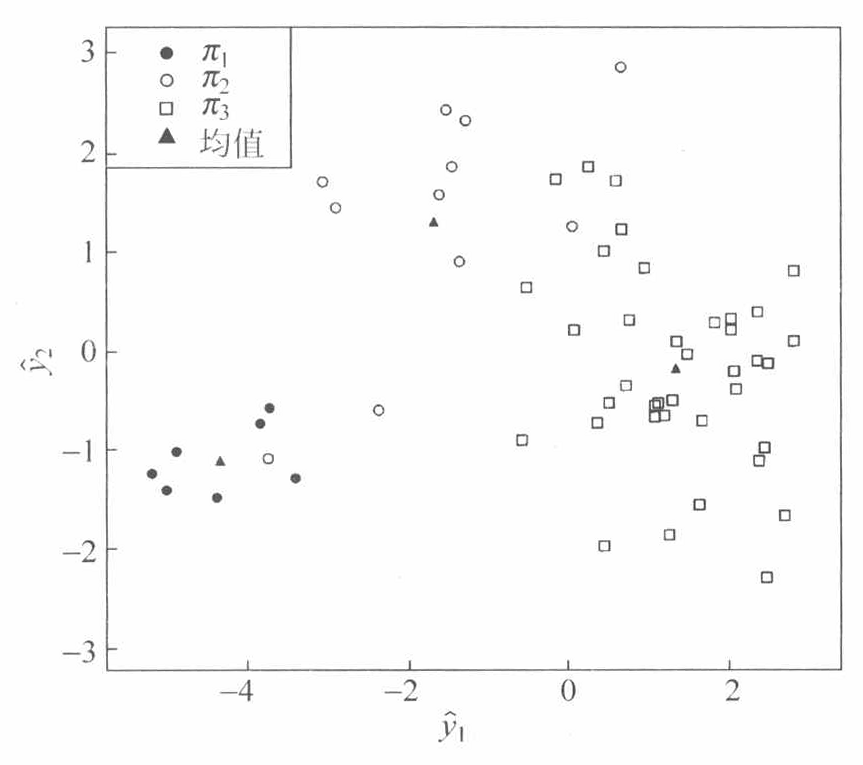
\includegraphics[width=73.1mm]{figs/fig_pg499_1.png}
\phantomsection\label{fig:11.12}\mvcap{图 11.12\quad 判别空间中的原油数据散布图}
\end{mvfigure}

\noindent\textbf{例 11.15}\quad (将运动数据在二维判别空间作图)

一批研究人员对运动心理学感兴趣, 他们利用明尼苏达多重性格记录库(MMPI)中保存的威斯康星大学 670 名获奖选手的数据进行分析. 有关的运动项目及两个判别函数的系数列于\hyperref[tab:11.3]{表 11.3}.

%% ===== pg-500 =====

% ---- pg-500 （书页 488） ----

\begin{mvtable}
\phantomsection\label{tab:11.3}\mvtabcap{表 11.3}
\begin{tabular}{cc||ccc}
\toprule
运动 & 样本容量 & MMPI 指标 & 第一判别量 & 第二判别量 \\
\midrule
足球 & 158 & QE & 0.055 & $-0.098$ \\
篮球 & 42 & L & $-0.194$ & 0.046 \\
棒球 & 79 & F & $-0.047$ & $-0.099$ \\
赛艇 & 61 & K & 0.053 & $-0.017$ \\
击剑 & 50 & Hs & 0.077 & $-0.076$ \\
高尔夫 & 28 & D & 0.049 & 0.183 \\
体操 & 26 & Hy & $-0.028$ & 0.031 \\
曲棍球 & 28 & Pd & 0.001 & $-0.069$ \\
游泳 & 51 & Mf & $-0.074$ & $-0.076$ \\
网球 & 31 & Pa & 0.189 & 0.088 \\
田径 & 52 & Pt & 0.025 & $-0.188$ \\
摔跤 & 64 & Sc & $-0.046$ & 0.088 \\
 &  & Ma & $-0.103$ & 0.053 \\
 &  & Si & 0.041 & 0.016 \\
\bottomrule
\end{tabular}
\end{mvtable}

{\zihao{6} 资料来源：W. Morgan 和 R. W. Johnson.}

用前两个判别得分得出的组均值图示于\hyperref[fig:11.13]{图 11.13}. 这里, 虽然对均值相等的检验在 5\% 的水平下显著, 但基于 MMPI 得分的分离却不好(这是由于大样本容量).

\begin{mvfigure}
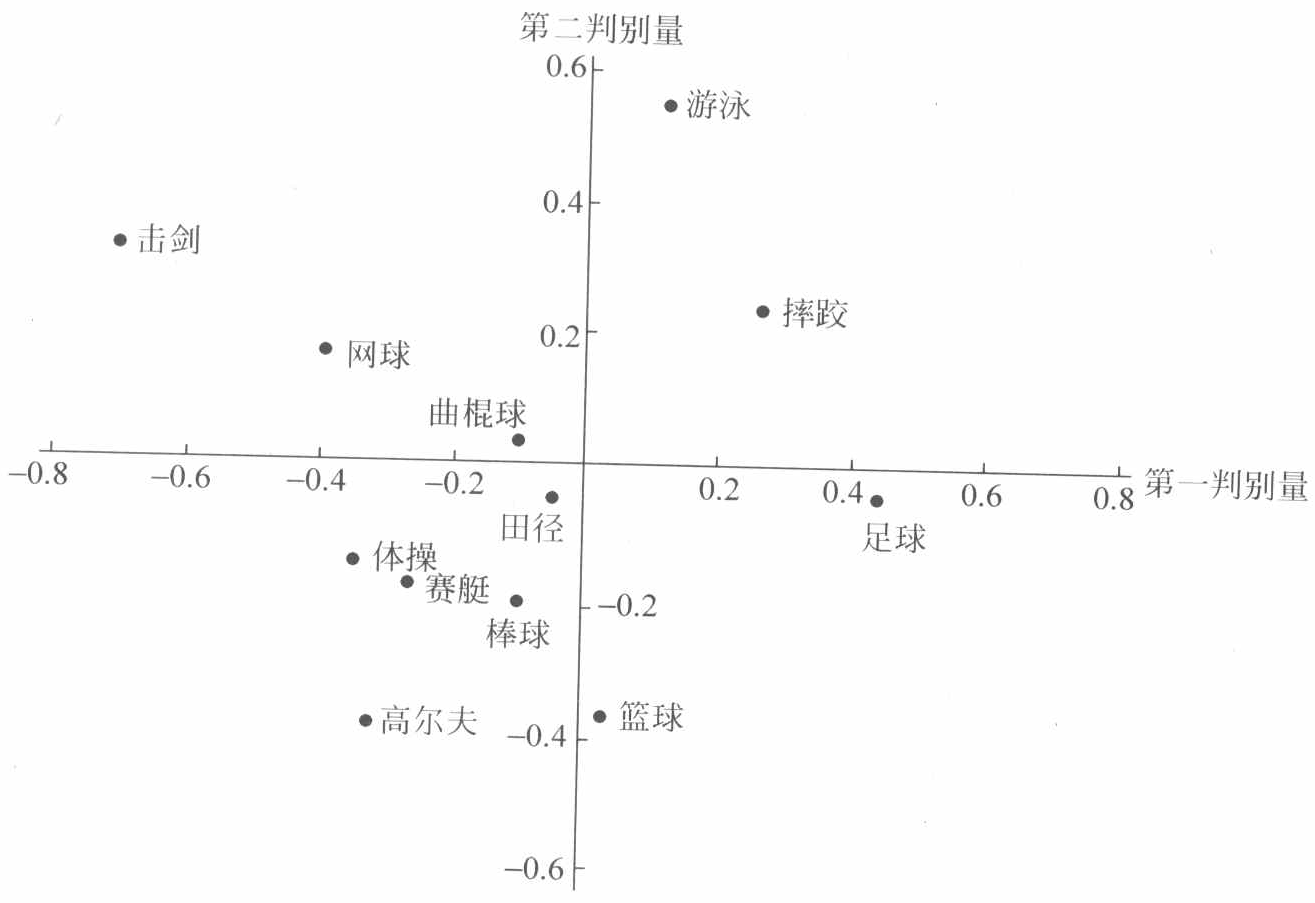
\includegraphics[width=111.3mm]{figs/fig_pg500_1.png}
\phantomsection\label{fig:11.13}\mvcap{图 11.13\quad 每项运动的判别均值 $\bar{y}'=[\bar{y}_1,\bar{y}_2]$}
\end{mvfigure}

然而判别系数却暗示: 第一判别量与 L 和 Ma 两个指标关系最密切, 而第二判别量则与 D 和 Pt 两个指标关系最密切. 下面给出这些研究人员所提供的解释.

第一判别量占总方差的 34.4\%, 它与 Mf 指标高度相关($r=-0.78$). 第二判别量占总方差的 18.3\%, 与 Sc, F 和 D 指标高度相关($r=0.66,0.54$ 和 $0.50$). 这些研究者认为, 第一判别量最好地代表了兴趣, 而第二判别量则反映了心理调整.

%% ===== pg-501 =====

% ---- pg-501 （书页 489） ----

在理想情况下, 应该对标准化的判别函数系数进行考察, 以估计一个变量在存在其他变量情形下的重要性(见文献[29]). 相关系数只指示每个变量如何通过自身来区分各总体, 而忽略其他变量的贡献. 不幸的是, 在本例中是得不到标准化判别系数的.

一般来说, 还应该对前几个判别量中的其他各对变量作标绘图. 此外, 可以对每项运动制作其判别量的判别得分散布图. 在多元正态性假定下, 以判别均值向量 $\bar{y}$ 为中心的单位椭圆(圆)应包含比例约为
\[
P[(\mathbf{Y}-\boldsymbol{\mu}_Y)'(\mathbf{Y}-\boldsymbol{\mu}_Y)\le 1]=P[\chi_2^2\le 1]=0.39
\]
的判别空间上的点.\hfill$\blacksquare$

\section{用费希尔判别量将对象进行分类}
\phantomsection\label{sec:11.7}

推导费希尔判别量的目的, 是得出一个能将总体最大限度地分开的低维数据表示. 虽然这些判别量是出于分离的考虑而导出的, 它们也为分类法则提供了依据. 我们先利用总体判别量 $\mathbf{a}_k'\mathbf{X}$ 来解释二者之间的联系.

令
\phantomsection\label{eq:11-64}
\begin{equation}
Y_k=\mathbf{a}_k'\mathbf{X}=\text{第}\ k\ \text{个判别量},\qquad k\le s
\tag{11-64}
\end{equation}
我们得出结论: 对总体 $\pi_i$,
\[
\mathbf{Y}=\begin{bmatrix}Y_1\\Y_2\\\vdots\\Y_s\end{bmatrix}
\qquad\text{有均值向量}\qquad
\boldsymbol{\mu}_{iY}=\begin{bmatrix}\mu_{iY_1}\\\vdots\\\mu_{iY_s}\end{bmatrix}=\begin{bmatrix}\mathbf{a}_1'\boldsymbol{\mu}_i\\\vdots\\\mathbf{a}_s'\boldsymbol{\mu}_i\end{bmatrix}
\]
而对所有总体则有协方差矩阵 $\mathbf{I}$(见练习 11.21).

由于 $\mathbf{Y}$ 的各分量均有单位方差和零协方差, 所以 $\mathbf{Y}=\mathbf{y}$ 到 $\boldsymbol{\mu}_{iY}$ 的适当的平方距离为
\[
(\mathbf{y}-\boldsymbol{\mu}_{iY})'(\mathbf{y}-\boldsymbol{\mu}_{iY})=\sum_{j=1}^{s}(y_j-\mu_{iY_j})^2
\]
一个合理的分类法则是: 若 $\mathbf{y}$ 到 $\boldsymbol{\mu}_{kY}$ 的平方距离小于 $\mathbf{y}$ 到其他 $\boldsymbol{\mu}_{iY}(i\ne k)$ 的平方距离, 则将 $\mathbf{y}$ 指派给 $\pi_k$.

若只用 $r$ 个判别量来进行分类, 则相应法则为: 若
\phantomsection\label{eq:11-65}
\begin{equation}
\begin{aligned}
\sum_{j=1}^{r}(y_j-\mu_{kY_j})^2&=\sum_{j=1}^{r}[\mathbf{a}_j'(\mathbf{x}-\boldsymbol{\mu}_k)]^2\\
&\le\sum_{j=1}^{r}[\mathbf{a}_j'(\mathbf{x}-\boldsymbol{\mu}_i)]^2\qquad \text{对所有}\ i\ne k
\end{aligned}
\tag{11-65}
\end{equation}
则将 $\mathbf{x}$ 分到 $\pi_k$.

在将这种分类方法与 11.5 节中所讨论的分类方法相联系之前, 我们先进一步探讨对判别量个数的限制. 由练习 11.21 知
\[
s=\text{判别量个数}=\boldsymbol{\Sigma}^{-1}\mathbf{B}_\mu\ \text{或}\ \boldsymbol{\Sigma}^{-1/2}\mathbf{B}_\mu\boldsymbol{\Sigma}^{-1/2}\ \text{的非零特征值的个数}
\]
由于 $\boldsymbol{\Sigma}^{-1}\mathbf{B}_\mu$ 为 $p\times p$, 故 $s\le p$. 进一步, $g$ 个向量
\phantomsection\label{eq:11-66}
\begin{equation}
\boldsymbol{\mu}_1-\bar{\boldsymbol{\mu}},\boldsymbol{\mu}_2-\bar{\boldsymbol{\mu}},\cdots,\boldsymbol{\mu}_g-\bar{\boldsymbol{\mu}}
\tag{11-66}
\end{equation}
满足 $(\boldsymbol{\mu}_1-\bar{\boldsymbol{\mu}})+(\boldsymbol{\mu}_2-\bar{\boldsymbol{\mu}})+\cdots+(\boldsymbol{\mu}_g-\bar{\boldsymbol{\mu}})=g\bar{\boldsymbol{\mu}}-g\bar{\boldsymbol{\mu}}=\mathbf{0}$. 也就是说, 第一个差值 $\boldsymbol{\mu}_1-\bar{\boldsymbol{\mu}}$ 可以表示为后 $g-1$ 个差值的线性组合. \hyperref[eq:11-66]{式(11-66)}中的 $g$ 个向量的线性组合决定一个超平面, 其维数 $q\le g-1$. 取任一向量 $\mathbf{e}$ 垂直于每一个 $\boldsymbol{\mu}_i-\bar{\boldsymbol{\mu}}$, 因而也垂直于这个超平面, 可以得到

%% ===== pg-502 =====

% ---- pg-502 （书页 490） ----

\[
\mathbf{B}_\mu\mathbf{e}=\sum_{i=1}^{g}(\boldsymbol{\mu}_i-\bar{\boldsymbol{\mu}})(\boldsymbol{\mu}_i-\bar{\boldsymbol{\mu}})'\mathbf{e}=\sum_{i=1}^{g}(\boldsymbol{\mu}_i-\bar{\boldsymbol{\mu}})0=\mathbf{0}
\]
因此
\[
\boldsymbol{\Sigma}^{-1}\mathbf{B}_\mu\mathbf{e}=0\mathbf{e}
\]
共有 $p-q$ 个正交特征向量对应于零特征值. 这意味着有 $q$ 个或更少的非零特征值. 由于总有 $q\le g-1$, 非零特征值的个数 $s$ 必满足 $s\le\min(p,g-1)$.

于是, 如果下列条件满足, 则用二维图进行判别不会损失信息.

\begin{mvtable}
\begin{tabular}{c|c|c}
\toprule
变量个数 & 总体个数 & 判别量的最大个数 \\
\midrule
任意 $p$ & $g=2$ & 1 \\
任意 $p$ & $g=3$ & 2 \\
$p=2$ & 任意 $g$ & 2 \\
\bottomrule
\end{tabular}
\end{mvtable}

现在我们给出分类法则(11-65)与“正态理论”判别得分[见\hyperref[eq:11-49]{式(11-49)}]之间的重要关系:
\[
d_i(x)=\boldsymbol{\mu}_i'\boldsymbol{\Sigma}^{-1}x-\frac{1}{2}\boldsymbol{\mu}_i'\boldsymbol{\Sigma}^{-1}\boldsymbol{\mu}_i+\ln p_i
\]
或等价的$\left(\text{上式两端各加同一个常数}-\frac{1}{2}x'\boldsymbol{\Sigma}^{-1}x\right)$,
\[
d_i(x)-\frac{1}{2}x'\boldsymbol{\Sigma}^{-1}x=-\frac{1}{2}(x-\boldsymbol{\mu}_i)'\boldsymbol{\Sigma}^{-1}(x-\boldsymbol{\mu}_i)+\ln p_i
\]
\mvthm{结论 11.6}{设 $y_j=\mathbf{a}_j'\mathbf{x}$, 其中 $\mathbf{a}_j=\boldsymbol{\Sigma}^{-1/2}\mathbf{e}_j$, $\mathbf{e}_j$ 为 $\boldsymbol{\Sigma}^{-1/2}\mathbf{B}_\mu\boldsymbol{\Sigma}^{-1/2}$ 的一个特征向量. 此时
\[
\begin{aligned}
\sum_{j=1}^{p}(y_j-\mu_{iY_j})^2&=\sum_{j=1}^{p}[\mathbf{a}_j'(\mathbf{x}-\boldsymbol{\mu}_i)]^2=(x-\boldsymbol{\mu}_i)'\boldsymbol{\Sigma}^{-1}(x-\boldsymbol{\mu}_i)\\
&=-2d_i(x)+x'\boldsymbol{\Sigma}^{-1}x+2\ln p_i
\end{aligned}
\]
若 $\lambda_1\ge\cdots\ge\lambda_s>0=\lambda_{s+1}=\cdots=\lambda_p$, $\sum\limits_{j=s+1}^{p}(y_j-\mu_{iY_j})^2$ 对所有总体 $\pi_i(i=1,2,\cdots,g)$ 均为常数. 因此只有前 $s$ 个判别量 $y_j$, 或者说只有 $\sum\limits_{j=1}^{s}(y_j-\mu_{iY_j})^2$ 对分类有贡献.

还有, 若先验概率满足 $p_1=p_2=\cdots=p_g=1/g$, 则取 $r=s$ 时, 法则(11-65)等价于总体形式的最小 TPM 法则(11-52).}

\noindent\mvbold{证明}\quad 平方距离$(x-\boldsymbol{\mu}_i)'\boldsymbol{\Sigma}^{-1}(x-\boldsymbol{\mu}_i)=(x-\boldsymbol{\mu}_i)'\boldsymbol{\Sigma}^{-1/2}\boldsymbol{\Sigma}^{-1/2}(x-\boldsymbol{\mu}_i)=(x-\boldsymbol{\mu}_i)'\boldsymbol{\Sigma}^{-1/2}\mathbf{E}\mathbf{E}'\boldsymbol{\Sigma}^{-1/2}(x-\boldsymbol{\mu}_i)$, 其中 $\mathbf{E}=[\mathbf{e}_1,\mathbf{e}_2,\cdots,\mathbf{e}_p]$ 为正交矩阵, 其列由 $\boldsymbol{\Sigma}^{-1/2}\mathbf{B}_\mu\boldsymbol{\Sigma}^{-1/2}$ 的特征向量构成(见练习 11.21).

因为 $\boldsymbol{\Sigma}^{-1/2}\mathbf{e}_j=\mathbf{a}_j$ 或 $\mathbf{a}_j'=\mathbf{e}_j'\boldsymbol{\Sigma}^{-1/2}$, 所以
\[
\mathbf{E}'\boldsymbol{\Sigma}^{-1/2}(x-\boldsymbol{\mu}_i)=\begin{bmatrix}\mathbf{a}_1'(x-\boldsymbol{\mu}_i)\\\mathbf{a}_2'(x-\boldsymbol{\mu}_i)\\\vdots\\\mathbf{a}_p'(x-\boldsymbol{\mu}_i)\end{bmatrix}
\]
且
\[
(x-\boldsymbol{\mu}_i)'\boldsymbol{\Sigma}^{-1/2}\mathbf{E}\mathbf{E}'\boldsymbol{\Sigma}^{-1/2}(x-\boldsymbol{\mu}_i)=\sum_{j=1}^{p}[\mathbf{a}_j'(x-\boldsymbol{\mu}_i)]^2
\]
然后, 每个 $\mathbf{a}_j=\boldsymbol{\Sigma}^{-1/2}\mathbf{e}_j(j>s)$ 为 $\boldsymbol{\Sigma}^{-1}\mathbf{B}_\mu$ 的一个(未标准化的)特征向量, 对应零特征值. 正

%% ===== pg-503 =====

% ---- pg-503 （书页 491） ----

如在\hyperref[eq:11-66]{式(11-66)}之后所讨论的, $\mathbf{a}_j$ 垂直于每个 $\boldsymbol{\mu}_i-\bar{\boldsymbol{\mu}}$, 因此也垂直于 $(\boldsymbol{\mu}_k-\bar{\boldsymbol{\mu}})-(\boldsymbol{\mu}_i-\bar{\boldsymbol{\mu}})=\boldsymbol{\mu}_k-\boldsymbol{\mu}_i$, $i,k=1,2,\cdots,g$. 条件 $0=\mathbf{a}_j'(\boldsymbol{\mu}_k-\boldsymbol{\mu}_i)=\mu_{kY_j}-\mu_{iY_j}$ 意味着, $y_j-\mu_{kY_j}=y_j-\mu_{iY_j}$, 故 $\sum\limits_{j=s+1}^{p}(y_j-\mu_{iY_j})^2$ 对 $i=1,2,\cdots,g$ 为常数. 因此, 只有前 $s$ 个判别量 $y_j$ 对分类有用.\hfill$\blacksquare$

现在我们陈述基于前 $r\le s$ 个样本判别量的分类法则.

\begin{mvframe}[基于样本判别量的费希尔分类方法]
若
\phantomsection\label{eq:11-67}
\begin{equation}
\sum_{j=1}^{r}(\hat{y}_j-\bar{y}_{kj})^2=\sum_{j=1}^{r}[\hat{\mathbf{a}}_j'(\mathbf{x}-\bar{\mathbf{x}}_k)]^2\le\sum_{j=1}^{r}[\hat{\mathbf{a}}_j'(\mathbf{x}-\bar{\mathbf{x}}_i)]^2\qquad \text{对所有}\ i\ne k
\tag{11-67}
\end{equation}
则将 $\mathbf{x}$ 分入 $\pi_k$, 其中 $\hat{\mathbf{a}}_j$ 由\hyperref[eq:11-62]{式(11-62)}中定义, $\bar{y}_{kj}=\hat{\mathbf{a}}_j'\bar{\mathbf{x}}_k$ 且 $r\le s$.
\end{mvframe}

当先验概率满足 $p_1=p_2=\cdots=p_g=1/g$ 且 $r=s$ 时, 法则(11-67)等价于法则(11-52), 后者根据最大线性判别得分得出. 此外, 若用 $r<s$ 个判别量进行分类, 则对每个总体 $\pi_i$ 来说, 平方距离或得分都要损失 $\sum\limits_{j=r+1}^{p}[\hat{\mathbf{a}}_j'(\mathbf{x}-\bar{\mathbf{x}}_i)]^2$, 此处 $\sum\limits_{j=r+1}^{s}[\hat{\mathbf{a}}_j'(\mathbf{x}-\bar{\mathbf{x}}_i)]^2$ 为对分类有用的部分.

\noindent\textbf{例 11.16}\quad (用费希尔判别量将一个新观测值分类)

我们采用例 11.13 中的费希尔判别量
\[
\hat{y}_1=\hat{\mathbf{a}}_1'\mathbf{x}=0.386x_1+0.495x_2
\]
\[
\hat{y}_2=\hat{\mathbf{a}}_2'\mathbf{x}=0.938x_1-0.112x_2
\]
根据\hyperref[eq:11-67]{式(11-67)}来对新观测值 $\mathbf{x}_0'=[1,3]$ 进行分类.

将 $\mathbf{x}_0'=[x_{01},x_{02}]=[1,3]$ 代入上述判别量, 就有
\[
\hat{y}_1=0.386x_{01}+0.495x_{02}=0.386\times 1+0.495\times 3=1.87
\]
\[
\hat{y}_2=0.938x_{01}-0.112x_{02}=0.938\times 1-0.112\times 3=0.60
\]
此外, $\bar{y}_{kj}=\hat{\mathbf{a}}_j'\bar{\mathbf{x}}_k$, 故(见例 11.13)
\[
\bar{y}_{11}=\hat{\mathbf{a}}_1'\bar{\mathbf{x}}_1=[0.386\quad 0.495]\begin{bmatrix}-1\\3\end{bmatrix}=1.10
\]
\[
\bar{y}_{12}=\hat{\mathbf{a}}_2'\bar{\mathbf{x}}_1=[0.938\quad -0.112]\begin{bmatrix}-1\\3\end{bmatrix}=-1.27
\]
类似地有
\[
\bar{y}_{21}=\hat{\mathbf{a}}_1'\bar{\mathbf{x}}_2=2.37
\]
\[
\bar{y}_{22}=\hat{\mathbf{a}}_2'\bar{\mathbf{x}}_2=0.49
\]
\[
\bar{y}_{31}=\hat{\mathbf{a}}_1'\bar{\mathbf{x}}_3=-0.99
\]
\[
\bar{y}_{32}=\hat{\mathbf{a}}_2'\bar{\mathbf{x}}_3=0.22
\]
最后, 必须识别
\[
\sum_{j=1}^{2}(\hat{y}_j-\bar{y}_{kj})^2=\sum_{j=1}^{2}[\hat{\mathbf{a}}_j'(\mathbf{x}-\bar{\mathbf{x}}_k)]^2
\]
对 $k=1,2,3$ 的最小值. 利用以上数字得到
\[
\sum_{j=1}^{2}(\hat{y}_j-\bar{y}_{1j})^2=(1.87-1.10)^2+(0.60+1.27)^2=4.09
\]

%% ===== pg-504 =====

% ---- pg-504 （书页 492） ----

\[
\sum_{j=1}^{2}(\hat{y}_j-\bar{y}_{2j})^2=(1.87-2.37)^2+(0.60-0.49)^2=0.26
\]
\[
\sum_{j=1}^{2}(\hat{y}_j-\bar{y}_{3j})^2=(1.87+0.99)^2+(0.60-0.22)^2=8.32
\]
由于当 $k=2$ 时得到 $\sum\limits_{j=1}^{2}(\hat{y}_j-\bar{y}_{kj})^2$ 的最小值, 我们将 $\mathbf{x}_0$ 分配到总体 $\pi_2$. \hyperref[fig:11.14]{图 11.14} 是用分类量 $\hat{y}_i(i=1,2,3)$ 解释这种情况的示意图.\hfill$\blacksquare$

\begin{mvfigure}
\begin{tikzpicture}[scale=1.25,font=\small]
\draw[->] (-1.75,0)--(3.95,0);
\draw[->] (0,-1.95)--(0,2.75);
\foreach \x in {-1,1,2,3}{\draw (\x,0)--(\x,-0.12) node[below]{$\x$};}
\foreach \y in {-1,1,2}{\draw (0,\y)--(-0.12,\y) node[left]{$\y$};}
\node[right] at (3.98,-0.02) {$\hat{y}_1$};
\node[left] at (-0.15,2.72) {$\hat{y}_2$};
\draw (1.79,0.62) .. controls (1.95,1.18) and (2.32,1.12) .. (2.43,0.41);
\node at (2.55,0.98) {最小距离};
\fill (-0.9,0.27) circle (1.4pt);
\node[right] at (-0.8,0.27) {$\bar{y}_3$};
\fill (1.79,0.62) circle (1.4pt);
\node[above left] at (1.76,0.68) {$\hat{y}$};
\fill (2.43,0.41) circle (1.4pt);
\node[right] at (2.53,0.41) {$\bar{y}_2$};
\fill (1.13,-1.23) circle (1.4pt);
\node[right] at (1.23,-1.23) {$\bar{y}_1$};
\end{tikzpicture}
\phantomsection\label{fig:11.14}\mvcap{图 11.14\quad 分类平面上的点 $\hat{y}'=[\hat{y}_1,\hat{y}_2]$, $\bar{y}_1'=[\bar{y}_{11},\bar{y}_{12}]$, $\bar{y}_2'=[\bar{y}_{21},\bar{y}_{22}]$ 和 $\bar{y}_3'=[\bar{y}_{31},\bar{y}_{32}]$}
\end{mvfigure}

\noindent\mvbold{评注}\quad 当两个线性判别函数被用于分类时, 观测值被指派给基于二维判别空间中欧氏距离的总体.

到目前为止, 我们尚未说明为什么前几个判别量比后几个更重要. 判别量的相对重要性由它们对分离总体的数值度量的贡献来确定. 考虑分离度量
\phantomsection\label{eq:11-68}
\begin{equation}
\Delta_S^2=\sum_{i=1}^{g}(\boldsymbol{\mu}_i-\bar{\boldsymbol{\mu}})'\boldsymbol{\Sigma}^{-1}(\boldsymbol{\mu}_i-\bar{\boldsymbol{\mu}})
\tag{11-68}
\end{equation}
其中
\[
\bar{\boldsymbol{\mu}}=\frac{1}{g}\sum_{i=1}^{g}\boldsymbol{\mu}_i
\]
且 $(\boldsymbol{\mu}_i-\bar{\boldsymbol{\mu}})'\boldsymbol{\Sigma}^{-1}(\boldsymbol{\mu}_i-\bar{\boldsymbol{\mu}})$ 为第 $i$ 个总体的均值 $\boldsymbol{\mu}_i$ 到中心 $\bar{\boldsymbol{\mu}}$ 的平方统计距离. 可以证明(见练习 11.22), $\Delta_S^2=\lambda_1+\lambda_2+\cdots+\lambda_p$(此处 $\lambda_1\ge\lambda_2\ge\cdots\ge\lambda_s$)为 $\boldsymbol{\Sigma}^{-1}\mathbf{B}$(或 $\boldsymbol{\Sigma}^{-1/2}\mathbf{B}\boldsymbol{\Sigma}^{-1/2}$)的非零特征值, 而 $\lambda_{s+1},\cdots,\lambda_p$ 则为零特征值.

由 $\Delta_S^2$ 给出的分离度可以用判别量均值来重新表示. 第一个判别量 $Y_1=\mathbf{e}_1'\boldsymbol{\Sigma}^{-1/2}\mathbf{X}$ 有均值 $\mu_{iY_1}=\mathbf{e}_1'\boldsymbol{\Sigma}^{-1/2}\boldsymbol{\mu}_i$, 且从 $\mu_{iY_1}$ 到中心值 $\bar{\mu}_{Y_1}=\mathbf{e}_1'\boldsymbol{\Sigma}^{-1/2}\bar{\boldsymbol{\mu}}$ 的平方距离为 $\lambda_1$(见练习 11.22). 由于 $\Delta_S^2$ 也可表示为
\[
\begin{aligned}
\Delta_S^2&=\lambda_1+\lambda_2+\cdots+\lambda_p\\
&=\sum_{i=1}^{g}(\boldsymbol{\mu}_{iY}-\bar{\boldsymbol{\mu}}_Y)'(\boldsymbol{\mu}_{iY}-\bar{\boldsymbol{\mu}}_Y)\\
&=\sum_{i=1}^{g}(\mu_{iY_1}-\bar{\mu}_{Y_1})^2+\sum_{i=1}^{g}(\mu_{iY_2}-\bar{\mu}_{Y_2})^2+\cdots+\sum_{i=1}^{g}(\mu_{iY_p}-\bar{\mu}_{Y_p})^2
\end{aligned}
\]
可以得出, 第一判别量对分离度量 $\Delta_S^2$ 有最大贡献 $\lambda_1$. 一般来说, 第 $r$ 个判别量 $Y_r=\mathbf{e}_r'\boldsymbol{\Sigma}^{-1/2}\mathbf{X}$ 对 $\Delta_S^2$ 的贡献为 $\lambda_r$. 若其余 $s-r$ 个非零特征值之和 $\lambda_{r+1}+\lambda_{r+2}+\cdots+\lambda_s$ 与前 $r$ 个非零特征值之和 $\lambda_1+\lambda_2+\cdots+\lambda_r$ 相比很小, 则后 $s-r$ 个判别量 $Y_{r+1},Y_{r+2},\cdots,Y_s$ 可以忽略, 而不会显著地影响分离总量. \footnote{关于进一步的最优降维性质见文献[18].}

对分类法则(11-67)的有效性目前所知不多. 由计算机生成的抽样实验提供了某些启示. 拉亨布鲁克(见文献[21])总结了一些特定情况下分类法则的表现. 为得出\hyperref[eq:11-65]{式(11-65)}中的总

%% ===== pg-505 =====

% ---- pg-505 （书页 493） ----

体结论, 要求有一个公共的协方差矩阵 $\boldsymbol{\Sigma}$. 若这一点是基本真实的, 且样本足够大, 则法则(11-67)应该表现相当好. 在任何情况下, 其性能可通过计算估计的失误率来检验. 具体来说, 应该计算由\hyperref[eq:11-57]{式(11-57)}给出的期望真实失误率的拉亨布鲁克估计值.

\section{逻辑斯蒂回归与分类}
\phantomsection\label{sec:11.8}

\subsection{引言}

前面讨论的分类函数是基于定量变量. 这里我们讨论一种分类方法, 其中某些或所有变量是定性的. 此方法称为逻辑斯蒂(logistic)回归. 在最简单的情况, 响应变量 $Y$ 只取两个值. 例如, $Y$ 可能是“男性”或“女性”, 或者“就业”或“失业”.

即使响应可能是两值的定性变量, 我们总可以将两个值记为 0 和 1. 例如, 可以令“男性”$=0$, “女性”$=1$. 则 1 的概率 $p$ 是我们感兴趣的参数. 此概率表示总体中标识为 1 的人所占比例. 分布的均值也是 $p$, 因为
\[
\text{均值}=0\times(1-p)+1\times p=p
\]
0 的比例为 $1-p$, 常记为 $q$.

分布的方差为
\[
\text{方差}=0^2\times(1-p)+1^2\times p-p^2=p(1-p)
\]
显然方差不是常数. 若 $p=0.5$, 则方差$=0.5\times 0.5=0.25$; 而当 $p=0.8$, 则方差$=0.8\times 0.2=0.16$. 当 $p$ 趋于 0 或 1 时, 方差趋于 0.

令响应 $Y$ 取值 0 或 1. 若我们要对取 1 的概率建立有一个预测变量的线性模型, 我们可以令
\[
p=E(Y\mid z)=\beta_0+\beta_1 z
\]
并再加上一个误差项 $\varepsilon$. 但是这个模型有严重缺陷.

\begin{itemize}
\item 由于线性函数是无界的, 因此响应 $Y$ 的预测值可能大于 1 或小于 0.
\item 回归分析的一个假定是: $Y$ 的方差关于预测变量 $Z$ 的所有值保持不变. 上面已经说明此假定在此不适合. 当然, 如果用加权的最小二乘法可以对此有适当改进.
\end{itemize}

我们需要其他方法将预测变量或协变量 $Z$ 引入模型(见文献[26]). 自此以后, 我们总在协变量的观测 $Z=z$ 给定的条件下对 $p(z)$ 建模, 即使实际上协变量是不固定的.

\subsection{逻辑模型}

不是直接对概率 $p$ 建立模型, 我们先考虑“机会比”(odds ratio)
\[
\mathrm{odds}=\frac{p}{1-p}
\]
即 1 的概率对 0 的概率之比. 注意: 与概率不同, 机会比可以大于 1. 若 80\% 的旅客的行李不被海关检查, 则 $p=0.8$, 则不被检查的机会是 $0.8/0.2=4$, 或 4 对 1. 但是机会比是不对称的, 因为被检查的机会是 $0.2/0.8=1/4$. 取自然对数, 我们得到 $\ln(4)=1.386$, 而 $\ln(1/4)=-1.386$, 刚好相差一个符号.

考虑机会比的自然对数, 其图像在\hyperref[fig:11.15]{图 11.15}. 当机会 $x$ 为 1, 即出现 0 或 1 的机会相同, 则 $x$ 的自然对数为 0. 当机会 $x$ 大于 1, 则自然对数随 $x$ 的增加而缓慢增加. 然而, 当机会 $x$ 小于 1, 则自然对数随 $x$ 的下降而迅速增加到 0.

在对于二值变量的逻辑斯蒂回归模型中, 我们对机会比的自然对数(称为 $p$ 的“logit”)建模.

%% ===== pg-506 =====

% ---- pg-506 （书页 494） ----

\begin{mvfigure}
\begin{tikzpicture}[x=0.42cm,y=0.62cm,font=\small]
\draw (0,-3.3)--(0,3.3);
\draw (0,0)--(10.6,0);
\foreach \y in {-3,-2,-1,1,2,3}{\draw (0,\y)--(-0.3,\y) node[left]{$\y$};}
\node[left] at (-0.3,0) {$0$};
\foreach \x in {2,4,6,8,10}{\draw (\x,0)--(\x,-0.22) node[below]{$\x$};}
\draw[domain=0.05:10,samples=120,smooth] plot (\x,{ln(\x)});
\node[rotate=90] at (-2.9,0) {$\ln(\text{odds})$};
\node at (5.5,-1.7) {odds $x$};
\end{tikzpicture}
\phantomsection\label{fig:11.15}\mvcap{图 11.15\quad 机会比的自然对数}
\end{mvfigure}

\phantomsection\label{eq:11-69}
\begin{equation}
\mathrm{logit}(p)=\ln(\mathrm{odds})=\ln\left(\frac{p}{1-p}\right)
\tag{11-69}
\end{equation}
在最简单的模型中, 我们假定 $\mathrm{logit}(p)$ 为预测变量 $Z$ 的线性函数, 即
\phantomsection\label{eq:11-70}
\begin{equation}
\mathrm{logit}(p)=\ln(\mathrm{odds})=\ln\left(\frac{p}{1-p}\right)=\beta_0+\beta_1 z
\tag{11-70}
\end{equation}
由于多数人习惯于用概率思考, 逻辑斯蒂模型可简单表示为
\[
\ln\left(\frac{p}{1-p}\right)=\beta_0+\beta_1 z
\]
先取两边的指数函数, 得到
\[
\theta(z)=\frac{p(z)}{1-p(z)}=\exp(\beta_0+\beta_1 z)
\]
其中 $\exp=\mathrm{e}=2.718$ 为自然对数的底. 再解出 $p(z)$, 得到
\phantomsection\label{eq:11-71}
\begin{equation}
p(z)=\frac{\exp(\beta_0+\beta_1 z)}{1+\exp(\beta_0+\beta_1 z)}
\tag{11-71}
\end{equation}
此函数描述逻辑斯蒂曲线. 概率 $p$ 与预测变量 $z$ 之间的关系不是线性的, 而是如\hyperref[fig:11.16]{图 11.16} 所示, 是一种 S 形曲线. 在\hyperref[fig:11.16]{图 11.16} 中, $\beta_0=-1,\beta_1=2$. 当 $z=0$ 时, 逻辑斯蒂函数的值为 $\exp(\beta_0)/[1+\exp(\beta_0)]$.

\begin{mvfigure}
\begin{tikzpicture}[x=2.0cm,y=1.9cm,font=\small]
\draw (0,0)--(0,1.08);
\draw (0,0)--(2.16,0);
\foreach \y/\lab in {0/0.0,0.2/0.2,0.27/0.27,0.4/0.4,0.6/0.6,0.8/0.8,0.95/0.95,1.0/1.0}{\draw (0,\y)--(-0.045,\y) node[left]{$\lab$};}
\foreach \xt in {0,0.5,1.0,1.5,2.0}{\draw (\xt,0)--(\xt,-0.035) node[below]{$\xt$};}
\draw[domain=0:2,samples=120,smooth] plot (\x,{exp(-1+2*\x)/(1+exp(-1+2*\x))});
\node[rotate=90] at (-0.30,0.5) {$p$};
\end{tikzpicture}
\phantomsection\label{fig:11.16}\mvcap{图 11.16\quad 逻辑斯蒂函数($\beta_0=-1,\beta_1=2$)}
\end{mvfigure}

%% ===== pg-507 =====

% ---- pg-507 （书页 495） ----

逻辑斯蒂曲线中的 $\beta_1$ 决定 $p$ 随 $z$ 变化的速度, 但是其解释并不如简单线性回归模型那么容易, 因为模型无论对于 $z$ 或 $\beta_1$ 都不是线性的. 尽管如此, 对于机会比, 我们可以得到线性关系.

综上所述, 逻辑斯蒂曲线可表为
\[
p(z)=\frac{\exp(\beta_0+\beta_1 z)}{1+\exp(\beta_0+\beta_1 z)}\qquad\text{或}\qquad p(z)=\frac{1}{1+\exp(-\beta_0-\beta_1 z)}
\]

\subsection{逻辑斯蒂回归分析}

考虑具有多个预测变量的模型. 令 $(z_{j1},z_{j2},\cdots,z_{jr})$ 为 $r$ 个预测变量的第 $j$ 次观测. 如同在线性回归的正态理论中一样, 通常令第一项系数为 1 并记 $\mathbf{z}_j=[1,z_{j1},z_{j2},\cdots,z_{jr}]'$. 在给定 $\mathbf{z}_j$ 的条件下, 我们假定观测 $Y_j$ 有成功概率 $p(\mathbf{z}_j)$ 的伯努利分布, 即
\[
P(Y_j=y_j)=p^{y_j}(\mathbf{z}_j)[1-p(\mathbf{z}_j)]^{1-y_j}\qquad y_j=0,1
\]
因此
\[
E(Y_j)=p(\mathbf{z}_j)\qquad \mathrm{Var}(Y_j)=p(\mathbf{z}_j)[1-p(\mathbf{z}_j)]
\]
在逻辑斯蒂模型中, 机会比的自然对数遵循线性模型. 特别地, 假定模型
\phantomsection\label{eq:11-72}
\begin{equation}
\ln\left(\frac{p(\mathbf{z}_j)}{1-p(\mathbf{z}_j)}\right)=\beta_0+\beta_1 z_{j1}+\cdots+\beta_r z_{jr}=\boldsymbol{\beta}'\mathbf{z}_j
\tag{11-72}
\end{equation}
其中 $\boldsymbol{\beta}=(\beta_0,\beta_1,\cdots,\beta_r)'$.

\quad\mvbold{极大似然估计}\quad 参数 $\boldsymbol{\beta}$ 可用极大似然法估计. 似然函数 $L$ 即在观测 $y_j, j=1,\cdots,n$ 的联合概率分布. 因此
\phantomsection\label{eq:11-73}
\begin{equation}
\begin{aligned}
L(\beta_0,\beta_1,\cdots,\beta_r)&=\prod_{j=1}^{n}p^{y_j}(\mathbf{z}_j)[1-p(\mathbf{z}_j)]^{1-y_j}\\
&=\frac{\prod\limits_{j=1}^{n}\mathrm{e}^{y_j(\beta_0+\beta_1 z_{j1}+\cdots+\beta_r z_{jr})}}{\prod\limits_{j=1}^{n}(1+\mathrm{e}^{\beta_0+\beta_1 z_{j1}+\cdots+\beta_r z_{jr}})}
\end{aligned}
\tag{11-73}
\end{equation}
其中 $p(\mathbf{z}_j)$ 满足\hyperref[eq:11-72]{式(11-72)}.

参数的极大似然估计不能表示成简单的封闭形式, 而是需要从一个初值开始, 通过数值迭代来得到似然函数的最大值. 技术上, 这种迭代程序称为迭代再加权最小二乘法(见文献[26]).

我们用 $\hat{\boldsymbol{\beta}}$ 记极大似然估计的数值解.

\quad\mvbold{参数的置信区间}\quad 当样本容量大时, $\hat{\boldsymbol{\beta}}$ 有渐近正态分布, 渐近均值为 $\boldsymbol{\beta}$, 渐近协方差矩阵为
\phantomsection\label{eq:11-74}
\begin{equation}
\widehat{\mathrm{Cov}}(\hat{\boldsymbol{\beta}})\approx\left[\sum_{j=1}^{n}\hat{p}(\mathbf{z}_j)(1-\hat{p}(\mathbf{z}_j))\mathbf{z}_j\mathbf{z}_j'\right]^{-1}
\tag{11-74}
\end{equation}
此矩阵的对角元的平方根分别为参数估计 $\hat{\beta}_0,\hat{\beta}_1,\cdots,\hat{\beta}_r$ 的标准差的估计, 即标准误差(SE). $\beta_k$ 的大样本 95\% 置信区间为
\phantomsection\label{eq:11-75}
\begin{equation}
\hat{\beta}_k\pm 1.96\,\mathrm{SE}(\hat{\beta}_k)\qquad k=0,1,\cdots,r
\tag{11-75}
\end{equation}
置信区间可用来检验每个单独的回归项在逻辑斯蒂模型中的显著性. 同样可以得到 $p(\mathbf{z}_j)$ 和 $\mathrm{logit}(p(\mathbf{z}_j))$ 的大样本置信区间. 详情见文献[17].

\quad\mvbold{似然比检验}\quad 对于有 $r$ 个预测变量加一个常数项的模型, 记最大化的似然为
\[
L_{\max}=L(\hat{\beta}_0,\hat{\beta}_1,\cdots,\hat{\beta}_r)
\]
若零假设为 $H_0:\beta_k=0$, 通过数值计算得到缩小模型下的极大似然估计和似然的极大值
\[
L_{\max,\mathrm{Reduced}}=L(\hat{\beta}_0,\hat{\beta}_1,\cdots,\hat{\beta}_{k-1},0,\hat{\beta}_{k+1},\cdots,\hat{\beta}_r)
\]

%% ===== pg-508 =====

% ---- pg-508 （书页 496） ----

在逻辑斯蒂回归分析中, 检验假设 $H_0$ 常用“负二倍对数似然比”
\phantomsection\label{eq:11-76}
\begin{equation}
-2\ln\left(\frac{L_{\max,\mathrm{Reduced}}}{L_{\max}}\right)
\tag{11-76}
\end{equation}
在这里称为“离差”(deviance). 其分布在假设 $H_0$ 成立时渐近收敛到自由度 1 的卡方分布. 对于大的离差值, 拒绝 $H_0$.

另一种检验单个回归项显著性的方法来自王尔德(Wald, 见文献[17]). 对假设 $H_0:\beta_k=0$, 王尔德检验的检验统计量为 $Z=\hat{\beta}_k/\mathrm{SE}(\hat{\beta}_k)$ 或自由度 1 的卡方分布形式 $Z^2$. 似然比检验优于王尔德检验, 因为似然比检验的显著性水平更接近于名义水平 $\alpha$.

一般的, 如果零假设中有 $m$ 个参数同时为 0, 对于缩减的模型, 离差的渐近分布为自由度 $m$ 的卡方分布.

对于单个的二值观测 $Y_j$, 残差
\[
\frac{Y_j-\hat{p}(\mathbf{z}_j)}{\sqrt{\hat{p}(\mathbf{z}_j)(1-\hat{p}(\mathbf{z}_j))}}
\]
只能取两个值, 因此不是特别有用. 较好的方法是将残差合理地分组, 然后对每组计算总残差. 如果在每组中有 $t$ 个残差, 求这些残差之和再除以 $\sqrt{t}$ 可以使得方差比较具有一致性.

以下我们给出逻辑斯蒂回归的细节和模型检验, 并给出其在分类中的应用.

\subsection{分类}

当观测单位属于总体 1 时, 令响应 $Y=1$; 而当观测单位属于总体 2 时, $Y=0$. (选择响应值取 1 和 0 是任意的, 但有方便性. 在例 11.17 中, 我们用 1 和 2.) 一旦建立起逻辑斯蒂回归函数, 并且有一组来自两个总体的训练样本, 我们可以进一步进行分类. 由于先验概率和代价不易结合到分析中去, 故采用以下分类准则:

\qquad 将 $\mathbf{z}$ 归入总体 1, 若估计的机会比大于 1, 即
\[
\frac{\hat{p}(\mathbf{z}_j)}{1-\hat{p}(\mathbf{z}_j)}=\exp\{\hat{\beta}_0+\hat{\beta}_1 z_{j1}+\cdots+\hat{\beta}_r z_{jr}\}>1
\]
等价的, 我们有简单线性判别准则:

\qquad 将 $\mathbf{z}$ 归入总体 1, 若线性判别函数大于 0, 即
\phantomsection\label{eq:11-77}
\begin{equation}
\ln\left(\frac{\hat{p}(\mathbf{z}_j)}{1-\hat{p}(\mathbf{z}_j)}\right)=\hat{\beta}_0+\hat{\beta}_1 z_{j1}+\cdots+\hat{\beta}_r z_{jr}>0
\tag{11-77}
\end{equation}

\noindent\textbf{例 11.17}\quad (鲑鱼数据的逻辑斯蒂回归)

在例 11.8 中我们引入了鲑鱼数据(\hyperref[tab:11.2]{表 11.2}). 在例 11.8 中, 我们在将鲑鱼分成阿拉斯加鲑鱼和加拿大鲑鱼时只依据年轮而忽略了性别. 如果性别数据也参与分析, 有可能得到更好的分类. 显示板 11.2 包含了用 SAS 软件对鲑鱼数据作逻辑斯蒂回归分析的输出. 这里, 对阿拉斯加鲑鱼 $Y=1$, 而对加拿大鲑鱼 $Y=2$. 预测变量(协变量)为性别(雌性 1, 雄性 2), 淡水生长和海水生长. 由 SAS 输出, 对全局零假设, 似然比检验的结果(缩减的模型只包含 $\beta_0$, 见\hyperref[eq:11-77]{式(11-77)})的显著性水平$<0.0001$. 因此在逻辑斯蒂模型中至少要有一个协变量. 在极大似然估计标题下查看每个个别项, 我们看到王尔德检验建议性别是不显著的($p$ 值$=0.7356$), 而淡水生长和海水生长两个协变量是显著的. 因此可以将性别从模型中去除, 此变量对分类没有意义. 逻辑斯蒂回归可以对不包含性别的模型再次分析, 最终得到的函数可依据判别法则(11-77)将鲑鱼分类为阿拉斯加鲑鱼或加拿大鲑鱼.

%% ===== pg-509 =====

% ---- pg-509 （书页 497） ----

但是我们仍然保留性别进行分类. 我们将鲑鱼 $j$ 分类为 1(阿拉斯加), 若线性分类函数
\[
\boldsymbol{\beta}'\mathbf{z}=3.5054+0.2816\ \text{性别}+0.1264\ \text{淡水生长}+0.0486\ \text{海水生长}\ge 0
\]
错误分类的观测见下表

\begin{mvtable}
\begin{tabular}{cccccc}
\toprule
行 & 总体 & 性别 & 淡水 & 海水 & 线性分类函数 \\
\midrule
2 & 1 & 1 & 131 & 355 & 3.093 \\
12 & 1 & 2 & 123 & 372 & 1.537 \\
13 & 1 & 1 & 123 & 372 & 1.255 \\
30 & 1 & 2 & 118 & 381 & 0.467 \\
51 & 2 & 1 & 129 & 420 & $-0.319$ \\
68 & 2 & 2 & 136 & 438 & $-0.028$ \\
71 & 2 & 2 & 90 & 385 & $-3.266$ \\
\bottomrule
\end{tabular}
\end{mvtable}

根据错误分类数据得到混淆矩阵:

\begin{mvtable}
\begin{tabular}{c|l|c|c|}
\multicolumn{2}{c}{} & \multicolumn{2}{c}{预测类属}\\
\multicolumn{2}{c}{} & \multicolumn{1}{c}{$\pi_1$: 阿拉斯加} & \multicolumn{1}{c}{$\pi_2$: 加拿大}\\ \cline{3-4}
\multirow{2}{*}{实际类属} & $\pi_1$: 阿拉斯加 & 46 & 4 \\ \cline{3-4}
 & $\pi_2$: 加拿大 & 3 & 47 \\ \cline{3-4}
\end{tabular}
\end{mvtable}

近似的误差率用百分比表示为
\[
\mathrm{APER}=\frac{4+3}{50+50}\times 100=7\%
\]
\hfill$\blacksquare$

在作逻辑斯蒂分类时, 最好使用折刀法(保留法)对误分类概率进行估计. 但是这种方法在通用的主要统计软件包中还没有.

\medskip
\noindent\textbf{显示板 11.2}\quad 利用 PROC LOGISTIC 对鲑鱼数据的 SAS 分析

\begin{mvbox}
{\ttfamily\small
title 'Logistic Regression and Discrimination';\hfill\textbf{\rmfamily PROGRAM COMMANDS}\\
data salmon;\\
infile 'T11-2.dat';\\
input country gender freshwater marine;\\
proc logistic desc;\\
model country = gender freshwater marine / expb;
\par}
\end{mvbox}

\begin{mvbox}
{\ttfamily\small
\hfill\textbf{OUTPUT}\\
\par\vspace{6pt}
{\centering\small Logistic Regression and Discrimination\par}
\vspace{4pt}
{\centering\small The LOGISTIC procedure\par}
\vspace{8pt}
{\centering\small Model Information\par}
\vspace{4pt}
{\centering\small
\begin{tabular}{ll}
Model & binary logit\\
\end{tabular}\par}
\vspace{8pt}
{\centering\small Response Profile\par}
\vspace{4pt}
{\centering\small
\begin{tabular}{lcc}
Ordered Value & country & \makecell{Total\\Frequency}\\
1 & 2 & 50\\
2 & 1 & 50\\
\end{tabular}\par}
\par}
\end{mvbox}

%% ===== pg-510 =====

% ---- pg-510 （书页 498） ----

\begin{mvframe}[显示板 11.2(续)]
{\small
{\centering Probability modeled is country $=2$.\\[2pt] Model Fit Statistics\par}
\vspace{6pt}
{\centering
\begin{tabular}{lcc}
 & Intercept & Intercept\\
 & Only & and\\
Criterion & & Covariates\\
AIC & 140.629 & 46.674\\
SC & 143.235 & 57.094\\
-2 Log L & 138.629 & 38.674\\
\end{tabular}\par}
\vspace{10pt}
{\centering Testing Global Null Hypothesis: BETA $=0$\par}
\vspace{4pt}
{\centering
\begin{tabular}{lccc}
Test & Chi-Square & DF & Pr $>$ ChiSq\\
\hline
Likelihood Ratio & 99.9557 & 3 & $<.0001$\\
Wald & 19.4435 & 3 & 0.0002\\
\hline
\end{tabular}\par}
\vspace{10pt}
{\centering The LOGISTIC Procedure\par}
\vspace{6pt}
{\centering Analysis of Maximum Likelihood Estimates\par}
\vspace{4pt}
{\centering
\begin{tabular}{lcccccc}
Parameter & DF & Estimate & \makecell{Standard\\Error} & \makecell{Wald\\Chi-Square} & Pr $>$ ChiSq & Exp (Est)\\
\hline
Intercept & 1 & 3.5054 & 6.3935 & 0.3006 & 0.5835 & 33.293\\
gender & 1 & 0.2816 & 0.8338 & 0.1140 & 0.7356 & 1.325\\
freshwater & 1 & 0.1264 & 0.0357 & 12.5423 & 0.0004 & 1.135\\
marine & 1 & $-0.0486$ & 0.0146 & 11.1460 & 0.0008 & 0.953\\
\hline
\end{tabular}\par}
}
\end{mvframe}

我们还可以在例 11.17 中去掉性别, 对淡水生长和海水生长两个预测变量作逻辑斯蒂回归分析. 但是, 与具有相同协方差阵的正态分布相比, 逻辑斯蒂分类的效率要低得多(见文献[17]).

\subsection{二项分布响应的逻辑斯蒂回归}

现在我们考虑稍微一般一些的情况. 假定有些观测是在相同的协变量 $\mathbf{z}_j$ 下得到的, 并假定总共有 $m$ 个数据集, 其中每个数据集内的预测变量相同. 当在预测变量 $\mathbf{z}_j$ 下作 $n_j$ 次独立试验, 响应 $Y_j$(译者注: $n_j$ 次试验中响应为 1 的频数)有二项分布, 成功概率为 $p(\mathbf{z}_j)=P(\text{成功}\mid \mathbf{z}_j)$.

由于 $Y_j$ 是独立的, $j=1,\cdots,m$, 因此似然函数表为乘积:
\phantomsection\label{eq:11-78}
\begin{equation}
L(\beta_0,\beta_1,\cdots,\beta_r)=\prod_{j=1}^{m}\binom{n_j}{y_j}p_j^{y_j}(\mathbf{z}_j)[1-p(\mathbf{z}_j)]^{n_j-y_j}
\tag{11-78}
\end{equation}
其中概率 $p(\mathbf{z}_j)$ 遵从逻辑模型(11-72).

极大似然估计 $\hat{\boldsymbol{\beta}}$ 没有封闭的函数形式, 只能得到数值解. 当样本的总容量足够大时, 渐近的协方差矩阵为
\phantomsection\label{eq:11-79}
\begin{equation}
\widehat{\mathrm{Cov}}(\hat{\boldsymbol{\beta}})\approx\left[\sum_{j=1}^{m}n_j\hat{p}(\mathbf{z}_j)(1-\hat{p}(\mathbf{z}_j))\mathbf{z}_j\mathbf{z}_j'\right]^{-1}
\tag{11-79}
\end{equation}
其中第 $i$ 个对角元为 $\hat{\beta}_{j+1}$ 的方差估计. 其平方根为标准误差 $\mathrm{SE}(\hat{\beta}_{j+1})$ 的大样本估计.

可以证明, 概率估计 $\hat{p}(\mathbf{z}_j)$ 的方差的大样本估计为

%% ===== pg-511 =====

% ---- pg-511 （书页 499） ----

\[
\widehat{\mathrm{Var}}(\hat{p}(\mathbf{z}_k))\approx(\hat{p}(\mathbf{z}_k))(1-\hat{p}(\mathbf{z}_k))^2\mathbf{z}_k'\left[\sum_{j=1}^{m}n_j\hat{p}(\mathbf{z}_j)(1-\hat{p}(\mathbf{z}_j))\mathbf{z}_j\mathbf{z}_j'\right]^{-1}\mathbf{z}_k
\]
考察以 $\hat{p}(\mathbf{z}_j)$ 为中心, 加减两倍标准误差估计的区间可能发现难于分类的观测(译者注: 此话语义不明).

\quad\mvbold{模型检定}\quad 一旦对数据拟合了一个模型, 最好要检定一下拟合的适合度. 为此应该提出以下问题.
\begin{itemize}
\item 是否存在数据对于拟合的逻辑斯蒂模型的系统偏离?
\item 是否存在一些不寻常的观测, 它们与数据的总体模式不一致(离群值)?
\item 是否存在一些观测, 当它们被包含在或被排除出数据时会导致统计分析结果发生重大差异(高影响点)?
\end{itemize}
如果单个的概率 $p(\mathbf{z}_j)=P(\text{成功}\mid \mathbf{z}_j)$ 没有参数结构, 则每个概率可以用观测的成功频数对于试验次数 $n_j$ 的比值来估计. 在此非参数模型或饱和模型下, 第 $j$ 个试验点对于似然的贡献为
\[
\binom{n_j}{y_j}p^{y_j}(\mathbf{z}_j)(1-p(\mathbf{z}_j))^{n_j-y_j}
\]
其最大值在 $\hat{p}(\mathbf{z}_j)=y_j/n_j$ 达到, $j=1,\cdots,n, m=\sum n_j$. 非参数(NP)负二倍最大化对数似然为
\phantomsection\label{eq:11-80}
\begin{equation}
-2\ln L_{\max,\mathrm{NP}}=-2\sum_{j=1}^{m}\left[y_j\ln\left(\frac{y_j}{n_j}\right)+(n_j-y_j)\ln\left(1-\frac{y_j}{n_j}\right)\right]+2\ln\left[\prod_{j=1}^{m}\binom{n_j}{y_j}\right]
\tag{11-80}
\end{equation}
其中右端最后一项对于所有模型都是一样的.

我们对于非参数模型与另外的包含一个常数项和 $r-1$ 个预测项的模型同样定义离差, 即负二倍对数似然比
\phantomsection\label{eq:11-81}
\begin{equation}
G^2=2\sum_{j=1}^{m}\left[y_j\ln\left(\frac{y_j}{\hat{y}_j}\right)+(n_j-y_j)\ln\left(\frac{n_j-y_j}{n_j-\hat{y}_j}\right)\right]
\tag{11-81}
\end{equation}
其中 $\hat{y}_j=n_j\hat{p}(\mathbf{z}_j)$ 为拟合的成功频数. 这是一种特殊的离差, 它的作用类似于线性模型中的残差平方和.

对于大的样本, $G^2$ 的渐近分布为卡方分布, 自由度 $f=m-r$, 其中 $m$ 为不同的试验点总数, $r$ 为拟合模型中参数的个数.

记全模型的离差为 $G^2_{\mathrm{Full}}$, 一个缩减模型的离差为 $G^2_{\mathrm{Reduced}}$, 则额外的预测项(译者注: 即包含在全模型中而不包含在缩减模型中的预测项)的贡献为
\phantomsection\label{eq:11-82}
\begin{equation}
G^2_{\mathrm{Reduced}}-G^2_{\mathrm{Full}}=-2\ln\left(\frac{L_{\max,\mathrm{Reduced}}}{L_{\max}}\right)
\tag{11-82}
\end{equation}
此差的渐近分布为卡方分布, 自由度 $\mathrm{df}=\mathrm{df}_{\mathrm{Reduces}}-\mathrm{df}_{\mathrm{Full}}$. 当此差有大的值, 意味着应考虑全模型.

当 $m$ 很大时, 在非参数模型中要估计的概率太多. 此时用现有的方法无法证明渐近卡方分布. 在这种场合, 最好以一个包含较少预测项的逻辑斯蒂模型作为基础进行似然比检验.

\quad\mvbold{残差与拟合优度检验}\quad 残差可用于检定数据的模式, 对逻辑模型的失拟合度和预测变量(协变量)的选择提出建议. 逻辑斯蒂回归模型中残差的定义不如在多重回归模型(第 7 章)中那样明确. 这里有三种不同的残差定义.

\qquad 离差残差($d_j$):

%% ===== pg-512 =====

% ---- pg-512 （书页 500） ----

\[
d_j=\pm\sqrt{2\left[y_j\ln\left(\frac{y_j}{n_j\hat{p}(\mathbf{z}_j)}\right)+(n_j-y_j)\ln\left(\frac{n_j-y_j}{n_j(1-\hat{p}(\mathbf{z}_j))}\right)\right]}
\]
其中 $d_j$ 的正负号与 $y_j-n_j\hat{p}(\mathbf{z}_j)$ 的正负号相同, 且
\phantomsection\label{eq:11-83}
\begin{equation}
\begin{aligned}
&\text{若}\ y_j=0,\ \text{则}\ d_j=-\sqrt{2n_j\left|\ln(1-\hat{p}(\mathbf{z}_j))\right|}\\
&\text{若}\ y_j=1,\ \text{则}\ d_j=-\sqrt{2n_j\left|\ln\hat{p}(\mathbf{z}_j)\right|}
\end{aligned}
\tag{11-83}
\end{equation}
皮尔逊(Pearson)残差($r_j$):
\phantomsection\label{eq:11-84}
\begin{equation}
r_j=\frac{y_j-n_j\hat{p}(\mathbf{z}_j)}{\sqrt{n_j\hat{p}(\mathbf{z}_j)(1-\hat{p}(\mathbf{z}_j))}}
\tag{11-84}
\end{equation}
标准化皮尔逊残差($r_{s_j}$):
\phantomsection\label{eq:11-85}
\begin{equation}
r_{s_j}=\frac{r_j}{\sqrt{1-h_{jj}}}
\tag{11-85}
\end{equation}
其中 $h_{jj}$ 为“帽子矩阵”$\mathbf{H}$ 的 $(j,j)$ 元, $\mathbf{H}$ 在\hyperref[eq:11-87]{式(11-87)}中给出. 大于约 2.5 的值表明在 $\mathbf{z}_j$ 失拟合度.

作为模型总体拟合优度检验统计量(对小样本特别适合), 皮尔逊卡方统计量为
\phantomsection\label{eq:11-86}
\begin{equation}
X^2=\sum_{j=1}^{m}r_j^2=\sum_{j=1}^{m}\frac{(y_j-n_j\hat{p}(\mathbf{z}_j))^2}{n_j\hat{p}(\mathbf{z}_j)(1-\hat{p}(\mathbf{z}_j))}
\tag{11-86}
\end{equation}
作为单一数值的拟合综合优度, 卡方统计量是皮尔逊残差的平方和. 直接考察皮尔逊残差本身也可以检定拟合的质量.

Hosmer 和 Lemeshow(见文献[17])提出另一种拟合优度检验方法. 但是这种方法仅适用于一定条件: 在相同的协变量值上只有少量的给出, 并且所有因变量(协变量)是连续的.

\mvsub{杠杆点与影响观测}\quad 在逻辑斯蒂模型中, 帽子矩阵 $\mathbf{H}$ 的等价概念包含估计的概率 $\hat{p}_k(\mathbf{z}_j)$.
\phantomsection\label{eq:11-87}
\begin{equation}
\mathbf{H}=\mathbf{V}^{-1/2}\mathbf{Z}(\mathbf{Z}'\mathbf{V}^{-1}\mathbf{Z})^{-1}\mathbf{Z}'\mathbf{V}^{-1/2}
\tag{11-87}
\end{equation}
其中 $\mathbf{V}^{-1}$ 为对角阵, $(j,j)$ 元为 $n_j\hat{p}(\mathbf{z}_j)(1-\hat{p}(\mathbf{z}_j))$, $\mathbf{V}^{-1/2}$ 为对角阵, $(j,j)$ 元为 $\sqrt{n_j\hat{p}(\mathbf{z}_j)(1-\hat{p}(\mathbf{z}_j))}$. 逻辑斯蒂回归版本的杠杆率为帽子矩阵 $\mathbf{H}$ 的对角元 $h_{jj}$.

除了由\hyperref[eq:11-87]{式(11-87)}给出的杠杆率外, 还有其他度量. 我们介绍一种最通用的度量, 称为 delta-beta 或删除替代(deletion displacement). 这个度量有助于辨识对于模式有强影响的观测. 从数据中删除所有对应 $\mathbf{z}_j$ 的观测, 回归系数的变化量为
\phantomsection\label{eq:11-88}
\begin{equation}
\Delta\boldsymbol{\beta}_j=\frac{r_{s_j}^2h_{jj}}{1-h_{jj}}
\tag{11-88}
\end{equation}
作 $\Delta\boldsymbol{\beta}_j$ 对 $j$ 的点图可用来检定有影响的观测点.

\section{最后的评述}  % 原书 11.8
\phantomsection\label{sec:11.9}

\mvsub{引入性质变量}

在本章中, 我们的讨论都假定判别或分类变量 $X_1,X_2,\cdots,X_p$ 有自然的度量单位. 也就是说, 每个变量原则上可以取任意实数, 且这些数值可以被记录. 性质变量或类别变量往往可以成为有用的判别量(分类量). 例如, 有或没有某种特性(如红色)可以是一个有价值的分类变量. 这种情况经常用如下方法处理: 定义一个变量 $X$, 当对象具有该特性时 $X$ 取值 1, 而当对

%% ===== pg-513 =====

% ---- pg-513 （书页 501） ----

象不具有该特性时 $X$ 取值 0. 于是这个变量在通常的判别和分类方法中就被作为一个被测量的变量来处理.

除了逻辑斯蒂回归, 当同时有连续变量和性质变量时, 分类问题几乎没有什么理论. 计算机模拟实验(见文献[22])表明, 费希尔的线性判别函数可能表现很差, 也可能表现得令人满意. 这取决于性质变量与连续变量之间的相关性. 正如克扎诺夫斯基(Krzanowski, 见文献[22])所指出的: “在一个总体中呈弱相关而在另一个总体中呈强相关, 或者两个总体之间的相关系数的符号改变, 这些都可能对费希尔线性判别函数不利的条件.” 这是一个麻烦的领域, 需要进一步研究.

\mvsub{分类树}

有人提出一种与本章前几节所介绍的方法完全不同的新的分类方法(见文献[5]). 这是一种计算机集成度高的方法, 因而只是到了现在才被广泛采用. 这个新方法称为\mvbold{分类与回归树}(CART), 与聚类技术有密切关系(见第 12 章).

起初, 所有对象被视为一个组. 根据某个变量的“高”值与“低”值, 将这个组分为两个子组. 然后再根据另一个变量分别将这两个子组再进行分组. 分离过程不断进行, 直到到达一个适当的停止点为止. 分离变量的值可以是有序类别, 也可以是无序类别. 正是这一特点使 CART 方法具有一般性.

例如, 假定人群被分类为
\[
\begin{aligned}
\pi_1&:\ \text{有心脏病发作倾向者}\\
\pi_2&:\ \text{无心脏病发作倾向者}
\end{aligned}
\]
分类变量为年龄、体重和运动量. 在这种情况下, CART 方法可用\hyperref[fig:11.17]{图 11.17} 中的树状图来表示. 树的分枝实际上对应样本空间中的分割. 区域 $R_1$ 的定义是年龄超过 45 岁, 超重, 且不经常锻炼的人群, 可用于将一个人分类为 $\pi_1$, 即有心脏病发作倾向者. CART 方法将尝试首先根据年龄, 或体重, 或运动量来进行分类.

\hyperref[fig:11.18]{图 11.18} 给出了用 CART 方法对鸢尾数据(见\hyperref[tab:11.5]{表 11.5})中变量 $X_3=$“花瓣长度”与 $X_4=$“花瓣宽度”的分类树. 图中指示了二项分裂法则. 例如, 第一次分裂出现在花瓣长度 $=2.45$. 花瓣长度 $\le 2.45$ 的构成第一组, 花瓣长度 $>2.45$ 的构成第二组.

\begin{mvfigure}
\begin{tikzpicture}[scale=0.82,every node/.style={font=\zihao{6}}]
\node[draw,ellipse] (a) at (0,0) {超过45岁};
\node[draw,ellipse] (b) at (-2.0,-1.5) {超重};
\node[draw,rectangle] (c) at (1.7,-1.5) {$\pi_2$};
\node[draw,ellipse] (d) at (-3.3,-3.0) {经常锻炼};
\node[draw,rectangle] (e) at (-1.2,-3.0) {$\pi_2$};
\node[draw,rectangle] (f) at (-4.5,-4.5) {$\pi_2$};
\node[draw,rectangle] (g) at (-2.1,-4.5) {$\pi_1$};
\draw (a)--(b);
\draw (a)--(c);
\draw (b)--(d);
\draw (b)--(e);
\draw (d)--(f);
\draw (d)--(g);
\node at (-1.35,-0.62) {是};
\node at (0.75,-0.62) {否};
\node at (-2.95,-2.12) {是};
\node at (-1.72,-2.12) {否};
\node at (-4.30,-3.62) {是};
\node at (-2.88,-3.62) {否};
\node[anchor=west] at (-4.5,-5.7) {$\pi_1$: 有心脏病发作倾向者};
\node[anchor=west] at (-4.5,-6.4) {$\pi_2$: 无心脏病发作倾向者};
\end{tikzpicture}
\phantomsection\label{fig:11.17}\mvcap{图 11.17\quad 分类树}
\end{mvfigure}

\begin{mvfigure}
\begin{tikzpicture}[scale=0.78,every node/.style={font=\zihao{6}}]
\node[diamond,draw,aspect=2.6,align=center] (n1) at (0,0) {Node 1\\PetLength\\N=150};
\node[draw,rectangle,align=center] (t1) at (-3.2,-2.4) {Terminal\\Node 1\\N=50};
\node[diamond,draw,aspect=2.6,align=center] (n2) at (2.6,-2.4) {Node 2\\PetWidth\\N=100};
\node[diamond,draw,aspect=2.6,align=center] (n3) at (0.5,-4.8) {Node 3\\PetLength\\N=54};
\node[draw,rectangle,align=center] (t4) at (4.4,-4.8) {Terminal\\Node 4\\N=46};
\node[draw,rectangle,align=center] (t2) at (-1.3,-7.2) {Terminal\\Node 2\\N=48};
\node[draw,rectangle,align=center] (t3) at (2.3,-7.2) {Terminal\\Node 3\\N=6};
\draw (n1.south west)--(t1.north);
\draw (n1.south east)--(n2.north);
\draw (n2.south west)--(n3.north);
\draw (n2.south east)--(t4.north);
\draw (n3.south west)--(t2.north);
\draw (n3.south east)--(t3.north);
\node at (0,1.15) {$\le 2.45$};
\node at (2.15,-1.25) {$\le 1.75$};
\node at (-0.55,-3.75) {$\le 4.95$};
\end{tikzpicture}
\phantomsection\label{fig:11.18}\mvcap{图 11.18\quad 鸢尾数据的分类树}
\end{mvfigure}

%% ===== pg-514 =====

% ---- pg-514 （书页 502） ----

下一次分裂出现在右手组(花瓣长度 $>2.45$), 花瓣宽度 $>1.75$ 构成另一组(右侧). 以上过程继续到没有更多的分裂为止. 过程在 4 个最终结(TN)停止.

二项分裂构成在 $X_3,X_4$ 样本空间的正象限(译者注: 第一象限)的最终结矩形(区域), 见\hyperref[fig:11.19]{图 11.19}. 例如, TN\#2 包含了 $2.45<$花瓣长度$\le 4.95$, 花瓣宽度 $\le 1.75$ 大的花, 主要是彩色花组.

\begin{mvfigure}
\begin{tikzpicture}[x=2.05cm,y=0.60cm,every node/.style={font=\zihao{6}}]
% 坐标框
\draw (0,1) rectangle (2.55,7);
\draw (1.75,1)--(1.75,7);
\draw (0,2)--(1.75,2);
\draw (0,5)--(1.75,5);
% y 轴刻度
\foreach \yy in {2,3,4,5,6,7} {\draw (-0.06,\yy)--(0,\yy); \node[left] at (-0.06,\yy) {\yy};}
\draw (-0.06,1)--(0,1); \node[left] at (-0.06,1) {1};
% x 轴刻度
\foreach \xx/\lab in {0/0.0,0.5/0.5,1.0/1.0,1.5/1.5,2.0/2.0,2.5/2.5} {\draw (\xx,1)--(\xx,0.93); \node[below] at (\xx,0.93) {\lab};}
% 分组标记
\draw plot[only marks,mark=x,mark size=1.6pt] coordinates{
(0.10,1.35)(0.15,1.55)(0.20,1.30)(0.22,1.75)(0.28,1.45)(0.30,1.90)(0.35,1.60)
(0.38,1.25)(0.42,1.75)(0.45,1.40)(0.50,1.85)(0.52,1.55)(0.55,1.30)(0.58,1.70)
(0.62,1.50)(0.65,1.90)(0.68,1.35)(0.25,1.15)(0.40,1.15)(0.58,1.15)};
\draw plot[only marks,mark=+,mark size=1.8pt] coordinates{
(0.95,3.45)(1.00,3.90)(1.00,3.10)(1.05,3.60)(1.05,4.20)(1.10,2.90)(1.10,3.85)
(1.15,4.30)(1.18,2.70)(1.20,3.30)(1.20,4.05)(1.25,4.50)(1.28,3.70)(1.30,4.75)
(1.32,4.15)(1.38,3.50)(1.40,4.40)(1.42,4.85)(1.45,3.90)(1.48,4.30)(1.52,4.60)
(1.55,4.45)(1.58,4.90)(1.62,4.20)(1.65,4.70)(1.50,3.60)};
\draw plot[only marks,mark=o,mark size=1.6pt] coordinates{
(1.80,5.20)(1.85,5.60)(1.85,4.60)(1.88,6.10)(1.90,4.90)(1.90,5.90)(1.92,4.30)
(1.95,5.30)(1.95,4.10)(1.95,6.30)(2.00,5.70)(2.00,6.60)(2.05,4.40)(2.05,6.90)
(2.10,5.00)(2.10,6.20)(2.15,5.50)(2.15,6.70)(2.20,4.70)(2.20,6.00)(2.25,5.30)
(2.28,6.40)(2.30,4.40)(2.35,5.60)(2.40,6.20)(2.40,4.10)(2.45,5.00)(2.45,6.50)
(2.50,4.60)(2.50,5.80)};
% 区域标注
\node at (0.32,5.65) {TN\#3};
\node at (0.32,4.35) {TN\#2};
\node at (1.22,1.50) {TN\#1};
\node at (2.18,3.60) {TN\#4};
% 轴标题
\node[rotate=90] at (-0.62,4.0) {PetLength};
\node at (1.28,0.30) {PetWidth};
% 图例
\draw (2.72,5.55) rectangle (3.45,7.35);
\node at (2.84,7.05) {$\times$}; \node at (3.06,7.05) {1}; \node at (3.30,7.05) {$\pi_1$};
\node at (2.84,6.45) {$+$};  \node at (3.06,6.45) {2}; \node at (3.30,6.45) {$\pi_2$};
\node at (2.84,5.85) {$\circ$}; \node at (3.06,5.85) {3}; \node at (3.30,5.85) {$\pi_3$};
\end{tikzpicture}
\phantomsection\label{fig:11.19}\mvcap{图 11.19\quad 在花瓣长度—花瓣宽度样本空间的分类树最终结(区域)}
\end{mvfigure}

由于在 TN\#3 中的花大部分属于 $\pi_3$, 这一组中的新项目将归入 $\pi_3$, 即 TN\#3 和 TN\#4 这两组都归入 $\pi_3$ 总体. 我们可以看到, CART 将所有 50 个 $\pi_1$ 品种正确分类, 将 50 个 $\pi_2$ 品种中 47 个正确分类, 将 50 个 $\pi_3$ 品种中 49 个正确分类. 因此 $\mathrm{APER}=\dfrac{4}{150}=0.027$, 这个结果与例 11.12 中用线性判别分析得到的结果大致相对.

CART 方法不依赖总体特征的概率分布, 也不依赖特定的最优性准则. 在实践中, 这种方法需要数百个对象和许多变量. 最后得出的树形图非常复杂, 必须利用主观判断对这棵树进行“修剪”, 使之终止于由若干对象构成的一些组, 而不是所有单个对象. 然后将每个终端组指派给含多数成员的总体, 而一个新对象则可根据其最后的组来分类.

为了实施 CART 分析, 布雷曼、弗里德曼、奥尔森和斯通(Breiman、Friedman、Olsen \& Stone, 见文献[5])开发了一个专用软件. 另外, Loh(见文献[21]和[25])开发了改进的分类树软件, 称为 QUEST\footnote{{\footnotesize 可在 \texttt{www.stat.wisc.edu/\textasciitilde loh/quest.html} 下载.}

\noindent{\footnotesize 可在 \texttt{www.stat.wisc.edu/\textasciitilde loh/cruise.html} 下载.}} 和 CRUISE\textsuperscript{\textcircled{2}}. 他们的程序中采用了若干个明智的分离法则, 通常能产生一棵有很好分离效果的树. CART 在数据挖掘中取得了很大成功(具补充材料 12A).

\mvsub{神经网络}

神经网络(NN)是一种计算机集成的算法过程, 它借助于由相对说比较简单的处理单元(神经元或节)高度连接而成的网络, 将输入转化为所需要的输出. 神经网络以人脑的神经活动为模型. 因此, 神经网络的三个基本特点为: 基本计算单元(神经元或节), 描述各计算单元之间连接状况的网络结构以及用来寻找完成特定工作所需的网络参数(权重)值的训练算法.

神经网络中的计算单元是互相连接的, 因为一个单元的输出可以是另一个单元的输入的一部分. 每个计算单元利用某种预先规定的函数将输入变换为输出, 这种变换在典型的情况下是单调的, 但在其他情况下则是任意的. 这个变换函数依赖于一些其值必须由输入和输出

%% ===== pg-515 =====

% ---- pg-515 （书页 503） ----

的训练集来确定的常数(参数).

网络结构是计算单元的组织形式及允许的连接类型. 在统计应用中, 计算单元被安排成若干层, 而且不同层的结点之间是连接的, 但在同一层中的结点不连接. 接受原始输入的层称为输入层, 最后一层称为输出层, 位于输入层和输出层之间的层统称为隐层. \hyperref[fig:11.20]{图 11.20} 是一个多层神经网络的简单示意图.

\begin{mvfigure}
\begin{tikzpicture}[scale=0.9,transform shape,
  nd/.style={circle,draw,minimum size=10mm,inner sep=0pt}]
% 输入层
\foreach \i/\x in {1/0,2/1.6,3/3.2,4/4.8}{
  \node[nd] (I\i) at (\x,0) {};
  \draw[-latex] (\x,-1.05)--(\x,-0.52);
  \node[below] at (\x,-1.0) {$X_{\i}$};
}
% 中间层(隐层)
\node[nd] (H1) at (1.6,1.9) {};
\node[nd] (H2) at (3.2,1.9) {};
% 输出层
\node[nd] (O1) at (0.8,3.8) {};
\node[nd] (O2) at (2.4,3.8) {};
\node[nd] (O3) at (4.0,3.8) {};
% 连接
\foreach \i in {1,...,4}{
  \draw (I\i)--(H1); \draw (I\i)--(H2);
}
\foreach \h in {1,2}{
  \draw (H\h)--(O1); \draw (H\h)--(O2); \draw (H\h)--(O3);
}
% 输出箭头
\foreach \x in {0.8,2.4,4.0}{
  \draw[-latex] (\x,4.35)--(\x,4.95);
}
% 层名
\node[anchor=east] at (-0.85,3.8) {输出层};
\node[anchor=east] at (-0.85,1.9) {中间层(隐层)};
\node[anchor=east] at (-0.85,0) {输入层};
\end{tikzpicture}
\phantomsection\label{fig:11.20}\mvcap{图 11.20\quad 有一个隐层的神经网络}
\end{mvfigure}

神经网络可用于判别和分类. 在这种应用中, 输入变量为所测量的总体特性量 $X_1,X_2,\cdots,X_p$, 而输出变量则为指示各组归属的类别变量. 最新的实践经验表明, 正确构造的神经网络其表现与本章中所讨论的逻辑斯谛回归和判别函数一样好. 文献[26]对神经网络在应用统计学中的运用提供了很好的讨论.

\mvsub{变量选择}

在判别分析的某些应用中, 可以获得大量变量的数据. 穆西阿迪和戈斯((Mucciardi \& Gose, 见文献[27])讨论了基于 157 个变量的判别分析.\footnote{想象一下验证关于 157 元正态性的假定和参数的联合估计问题, 或设想一下 $157\times 157$ 公共协方差阵中的 12\,403 个参数!} 在这种情况下, 显然希望选择一个包含较少变量, 同时又能保留与原集合几乎一样多信息的子集, 这就是逐步判别分析法的目标, 几个流行的商用计算机程序具有这种功能.

如果使用了逐步判别分析法(或任何一种变量选择方法), 则在解释其分析结果时必须小心(见文献[28]). 不管使用何种准则来选择变量, 所得到的变量子集不一定是最优的. 例如, 根据最小化表观误差率或最大化“判别能力”所得到的子集在用于未来样本时可能效果很差. 如果在各变量之间或变量的各线性组合之间存在强相关, 则与变量选择方法相联系的问题会变得更严重.

对给定的一个数据集, 若目标是分类, 则选择一个最优变量子集的问题变得特别麻烦. 至少, 导出的分类函数应该用一个有效的样本来评估. 正如默里(Murray, 见文献[28])所建议的那样, 将样本分成若干组并对每一组确定“最优”变量子集, 也许是较好的想法. 对一个给定的变量, 它在这些最优子集中出现的次数就是这个变量在未来分类中的价值度量.

\mvsub{检验组间的差别}

在两组数据的分类问题中我们已经指出, 除非两个总体分离得很好, 否则有效分配大概是不可能的. 对于两组以上数据, 情况也一样, 除非总体的均值向量之间有显著差别, 否则就不要做分类. 假定数据的分布接近多元正态分布, 且共有相同的协方差阵, 此时可用 MANOVA (多元方差分析)来检验总体均值向量之间的差别. 虽然表观的显著差别并不自动意味着有效的分类, 但检验是必要的第一步. 如果没有发现(总体均值的)显著差别, 则构造分类法则可能只是浪费时间.

\mvsub{图}

先进的计算机作图使人们现在可以用目测方法直观地考察二维或三维的多元数据. 这样,

%% ===== pg-516 =====

% ---- pg-516 （书页 504） ----

对任何两个或三个变量的数据在变量空间的分组情况, 都可以用肉眼来识别. 用这种方法往往能识别出潜在的重要分类变量, 并能揭示那些“离群的”或“非典型的”观测值. 可视性显示在判别和分类中是重要的辅助工具, 因而随着计算机硬件和有关计算机程序变得随手可得, 它们的应用也可能不断增加. 从视觉考察所获得的信息往往与通过复杂数值分析所得到的一样多.

\mvsub{关于多元正态性的实际考虑}

尝试性假定的选择与所得到的分离函数形式之间的相互作用是重要的. 考虑\hyperref[fig:11.21]{图 11.21}, 此图显示两个非正态密度的肾形轮廓线. 在这种情况下, 基于正态理论的线性(甚或二次)分类法则与另外一种选择相比就显得不适当了. 也就是说, 线性判别法在此处不适用.

\begin{mvfigure}
\begin{tikzpicture}[scale=0.95,transform shape]
% 坐标轴
\draw[->] (0,0)--(7.3,0) node[below right] {$x_1$};
\draw[->] (0,0)--(0,5.3) node[left] {$x_2$};
% 两个非正态总体的肾形轮廓线
\draw[thick] plot[smooth cycle,tension=0.9] coordinates {
(1.5,1.7) (1.7,2.5) (2.3,3.15) (3.0,3.35) (3.45,3.0)
(3.05,2.7) (2.6,2.45) (3.05,2.15) (3.5,1.9) (3.3,1.4)
(2.7,1.15) (2.0,1.2)};
\draw[thick] plot[smooth cycle,tension=0.9] coordinates {
(3.45,2.95) (4.05,3.6) (4.85,3.6) (5.35,3.1) (5.4,2.3)
(5.05,1.65) (4.35,1.3) (3.7,1.35) (3.35,1.7) (3.85,1.95)
(4.3,2.3) (3.9,2.65)};
% 分界线
\draw[dashed] (1.9,5.05)--(6.4,0.5);
\draw[dashed] (2.75,5.15)--(3.75,0.15);
% 标注
\node at (2.15,4.9) {\small “线性分类”的分界线};
\draw[->] (2.0,4.62)--(1.85,4.35);
\node at (4.6,4.6) {\small “良好分类”的分界线};
\draw[->] (3.95,4.38)--(3.35,4.12);
\node[align=center] at (0.62,2.95) {$f_2(x)$的\\轮廓线};
\draw[->] (1.55,3.0)--(1.85,2.9);
\node at (6.35,3.2) {\small $f_1(x)$的轮廓线};
\draw[->] (5.9,3.1)--(5.4,2.95);
\node at (1.5,0.85) {$R_2$};
\node at (5.95,1.4) {$R_1$};
\end{tikzpicture}
\phantomsection\label{fig:11.21}\mvcap{图 11.21\quad 线性判别不适用的两个非正态总体}
\end{mvfigure}

经常要对有很多变量的对象进行分类, 其中有些是“有—无”型或“0—1”型变量. 在这些情形或其他一些变量值域受限制的情形下, 多元正态性也许不是一个明智的假定. 如我们所知, 基于费希尔线性判别量的分类仅当多元正态性假定成立时才是最小 ECM 或最小 TPM 意义下的最优分类. 当正态性明显不成立时, 我们如何解释这些量?

在没有多元正态性的场合, 费希尔的线性判别量可以看成是对总样本信息提供了一种近似. 前几个判别量本身的正态性可以检验, 然后可以用法则(11-67). 由于判别量是大量变量的线性组合, 它们往往接近正态变量. 当然, 必须记住: 前几个判别量为原始样本信息的不完全汇总. 当根据全部样本信息导出的最优法则表现很好时, 基于这个受限制的判别量集合的分类法则也许表现很差.

\mvsub{练习}

\noindent 11.1\quad 考虑两个数据集
\[
\mathbf{X}_1=\begin{bmatrix}3&7\\2&4\\4&7\end{bmatrix}
\qquad\text{和}\qquad
\mathbf{X}_2=\begin{bmatrix}6&9\\5&7\\4&8\end{bmatrix}
\]
其中
\[
\bar{\mathbf{x}}_1=\begin{bmatrix}3\\6\end{bmatrix},\qquad
\bar{\mathbf{x}}_2=\begin{bmatrix}5\\8\end{bmatrix}
\]
及

%% ===== pg-517 =====

% ---- pg-517 （书页 505） ----

\[
\mathbf{S}_n=\begin{bmatrix}1&1\\1&2\end{bmatrix}
\]

(a) 计算\hyperref[eq:11-19]{式(11-19)}中的线性判别函数.

(b) 用法则(11-18), 在相同先验概率和相同代价下将观测值 $\mathbf{x}_0'=[2\quad 7]$ 分类到总体 $\pi_1$ 或总体 $\pi_2$.

\noindent 11.2\quad (a) 对例 11.1 中的数据, 用\hyperref[eq:11-19]{式(11-19)}得到一个线性判别函数.

(b) 利用(a)中得到的函数和\hyperref[eq:11-20]{式(11-20)}, 通过将给定观测值分类构造“模糊矩阵”. 将你的分类结果与\hyperref[fig:11.1]{图 11.1} 中的结果进行比较. 这里的分类域用目测法确定(见例 11.6).

(c) 给定(b)中的结果, 计算表观误分类率(APER).

(d) 陈述你在使用(a)和(b)中的方法时所根据的假定.

\noindent 11.3\quad 证明结论 11.1.

提示: 将\hyperref[eq:11-1]{式(11-1)}和\hyperref[eq:11-2]{式(11-2)}中所给的 $P(2\mid 1)$ 和 $P(1\mid 2)$ 的积分表达式代入\hyperref[eq:11-5]{式(11-5)}, 得到
\[
\mathrm{ECM}=c(2\mid 1)p_1\int_{R_2}f_1(\mathbf{x})d\mathbf{x}+c(1\mid 2)p_2\int_{R_1}f_2(\mathbf{x})d\mathbf{x}
\]
注意 $\Omega=R_1\cup R_2$, 故总概率
\[
1=\int_{\Omega}f_1(\mathbf{x})d\mathbf{x}=\int_{R_1}f_1(\mathbf{x})d\mathbf{x}+\int_{R_2}f_1(\mathbf{x})d\mathbf{x}
\]
可以将 ECM 写成
\[
\mathrm{ECM}=c(2\mid 1)p_1\left[1-\int_{R_2}f_1(\mathbf{x})d\mathbf{x}\right]+c(1\mid 2)p_2\int_{R_2}f_2(\mathbf{x})d\mathbf{x}
\]
由于积分的可加性, 有
\[
\mathrm{ECM}=\int_{R_2}\left[c(1\mid 2)p_2f_2(\mathbf{x})-c(2\mid 1)p_1f_1(\mathbf{x})\right]d\mathbf{x}+c(2\mid 1)p_1
\]
现在, $p_1$, $p_2$, $c(1\mid 2)$ 和 $c(2\mid 1)$ 皆为非负. 此外, $f_1(\mathbf{x})$ 和 $f_2(\mathbf{x})$ 对所有 $\mathbf{x}$ 均非负, 且在 ECM 中只有这两个量依赖于 $\mathbf{x}$. 这样, 若 $R_2$ 中只包含满足条件
\[
\left[c(1\mid 2)p_2f_2(\mathbf{x})-c(2\mid 1)p_1f_1(\mathbf{x})\right]\le 0
\]
的 $\mathbf{x}$ 而不包含使此量大于零的 $\mathbf{x}$, 则 ECM 达到最小.

\noindent 11.4\quad 一名研究人员想确定一种在两个多元总体之间进行判别的方法. 他能获得足够多的数据来估计分别与总体 $\pi_1$ 和 $\pi_2$ 相联系的密度函数 $f_1(\mathbf{x})$ 和 $f_2(\mathbf{x})$. 设 $c(2\mid 1)=50$(这是将 $\pi_1$ 中的观测值指定到 $\pi_2$ 中的代价)及 $c(1\mid 2)=100$.

此外, 已知大约有 20\% 的可能项目(可以记录它们的 $\mathbf{x}$ 测量值)属于 $\pi_1$.

(a) 给出将一个新的观测值分入两个总体之一的最小 ECM 法则(一般形式).

(b) 对一个新项目记录的测量值产生密度函数值 $f_1(\mathbf{x})=0.3$ 和 $f_2(\mathbf{x})=0.5$. 根据以上信息, 将此新项目分到 $\pi_1$ 或 $\pi_2$.

\noindent 11.5\quad 证明
\[
\begin{aligned}
&-\frac{1}{2}(\mathbf{x}-\boldsymbol{\mu}_1)'\boldsymbol{\Sigma}^{-1}(\mathbf{x}-\boldsymbol{\mu}_1)+\frac{1}{2}(\mathbf{x}-\boldsymbol{\mu}_2)'\boldsymbol{\Sigma}^{-1}(\mathbf{x}-\boldsymbol{\mu}_2)\\
&\quad=(\boldsymbol{\mu}_1-\boldsymbol{\mu}_2)'\boldsymbol{\Sigma}^{-1}\mathbf{x}-\frac{1}{2}(\boldsymbol{\mu}_1-\boldsymbol{\mu}_2)'\boldsymbol{\Sigma}^{-1}(\boldsymbol{\mu}_1+\boldsymbol{\mu}_2)
\end{aligned}
\]
[见\hyperref[eq:11-13]{式(11-13)}.]

%% ===== pg-518 =====

% ---- pg-518 （书页 506） ----

\noindent 11.6\quad 考虑线性函数 $Y=\mathbf{a}'\mathbf{X}$. 当 $\mathbf{X}$ 属于总体 $\pi_1$ 时, 记 $E(\mathbf{X})=\boldsymbol{\mu}_1$ 和 $\mathrm{Cov}(\mathbf{X})=\boldsymbol{\Sigma}$. 当 $\mathbf{X}$ 属于总体 $\pi_2$ 时, 记 $E(\mathbf{X})=\boldsymbol{\mu}_2$ 和 $\mathrm{Cov}(\mathbf{X})=\boldsymbol{\Sigma}$. 令 $m=\frac{1}{2}(\boldsymbol{\mu}_1+\boldsymbol{\mu}_2)=\frac{1}{2}(\mathbf{a}'\boldsymbol{\mu}_1+\mathbf{a}'\boldsymbol{\mu}_2)$. 给定 $\mathbf{a}'=(\boldsymbol{\mu}_1-\boldsymbol{\mu}_2)'\boldsymbol{\Sigma}^{-1}$, 证明下列结论:

(a) $E(\mathbf{a}'\mathbf{X}\mid \pi_1)-m=\mathbf{a}'\boldsymbol{\mu}_1-m>0$

(b) $E(\mathbf{a}'\mathbf{X}\mid \pi_2)-m=\mathbf{a}'\boldsymbol{\mu}_2-m<0$

提示: 回顾 $\boldsymbol{\Sigma}$ 是满秩的, 因而也是正定的, 故 $\boldsymbol{\Sigma}^{-1}$ 存在且正定.

\noindent 11.7\quad 设对 $|x|\le 1$, $f_1(x)=(1-|x|)$ 对 $-0.5\le x\le 1.5$, $f_2(x)=\frac{1}{2}(1-|x-0.5|)$.

(a) 对两个密度函数作图.

(b) 当 $p_1=p_2$ 和 $c(1\mid 2)=c(2\mid 1)$ 时, 确定分类域.

(c) 当 $p_1=0.2$ 和 $c(1\mid 2)=c(2\mid 1)$ 时, 确定分类域.

\noindent 11.8\quad 参看练习 11.7. 设 $f_1(x)$ 不变, 但取 $f_2(x)=\frac{1}{4}(2-|x-0.5|)$, $-1.5\le x\le 2.5$.

(a) 对两个密度函数作图.

(b) 当 $p_1=p_2$ 和 $c(1\mid 2)=c(2\mid 1)$ 时确定分类域.

\noindent 11.9\quad 对 $g=2$ 个总体, 证明\hyperref[eq:11-59]{式(11-59)}中的比值与下述比值成比例:
\[
\begin{aligned}
\frac{(\bar{Y}\text{ 的均值间的平方距离})}{(\bar{Y}\text{ 的方差})}&=\frac{(\mu_{1Y}-\mu_{2Y})^2}{\sigma_Y^2}=\frac{(\mathbf{a}'\boldsymbol{\mu}_1-\mathbf{a}'\boldsymbol{\mu}_2)^2}{\mathbf{a}'\boldsymbol{\Sigma}\mathbf{a}}\\
&=\frac{\mathbf{a}'(\boldsymbol{\mu}_1-\boldsymbol{\mu}_2)(\boldsymbol{\mu}_1-\boldsymbol{\mu}_2)'\mathbf{a}}{\mathbf{a}'\boldsymbol{\Sigma}\mathbf{a}}=\frac{(\mathbf{a}'\boldsymbol{\delta})^2}{\mathbf{a}'\boldsymbol{\Sigma}\mathbf{a}}
\end{aligned}
\]
其中 $\boldsymbol{\delta}=(\boldsymbol{\mu}_1-\boldsymbol{\mu}_2)$ 为均值向量之差. 该比值是\hyperref[eq:11-23]{式(11-23)}的总体对应量. 试证: 对任意 $c\ne 0$, 该比值通过下面的线性组合达到最大:
\[
\mathbf{a}=c\boldsymbol{\Sigma}^{-1}\boldsymbol{\delta}=c\boldsymbol{\Sigma}^{-1}(\boldsymbol{\mu}_1-\boldsymbol{\mu}_2)
\]
提示: 注意对 $i=1,2$, 有
\[
(\boldsymbol{\mu}_i-\boldsymbol{\mu})(\boldsymbol{\mu}_i-\boldsymbol{\mu})'=\frac{1}{4}(\boldsymbol{\mu}_1-\boldsymbol{\mu}_2)(\boldsymbol{\mu}_1-\boldsymbol{\mu}_2)',\quad \text{其中}\ \boldsymbol{\mu}=\frac{1}{2}(\boldsymbol{\mu}_1+\boldsymbol{\mu}_2).
\]

\noindent 11.10\quad 设 $n_1=11$ 个和 $n_2=12$ 个观测值分别取自两个随机变量 $X_1$ 和 $X_2$. 假定这两个变量服从二元正态分布, 且有相同的协方差矩阵, 但均值向量 $\boldsymbol{\mu}_1,\boldsymbol{\mu}_2$ 可能有差别. 样本均值向量和联合协方差矩阵为
\[
\bar{\mathbf{x}}_1=\begin{bmatrix}-1\\1\end{bmatrix};\qquad \bar{\mathbf{x}}_2=\begin{bmatrix}2\\1\end{bmatrix}
\]
\[
\mathbf{S}_n=\begin{bmatrix}7.3&-1.1\\-1.1&4.8\end{bmatrix}
\]

(a) 用霍特林二样本 $T^2$ 统计量检验总体均值向量是否有显著差别. 取 $\alpha=0.10$.

(b) 构造费希尔(样本)线性判别函数[见\hyperref[eq:11-19]{式(11-19)}和\hyperref[eq:11-25]{式(11-25)}].

(c) 将观测值 $\mathbf{x}_0'=[0\quad 1]$ 分配到总体 $\pi_1$ 或 $\pi_2$. 假定有等代价和等先验概率.

\noindent 11.11\quad 假定一维随机变量 $X$ 具有方差为 4 的正态分布. 若 $X$ 来自总体 $\pi_1$, 则其均值为 10; 而当它来自总体 $\pi_2$ 时, 其均值为 14. 假定事件 $A1=$“$X$ 来自 $\pi_1$”与事件 $A2=$“$X$ 来自 $\pi_2$”有相同的先验概率, 且错分代价 $c(2\mid 1)$ 与 $c(1\mid 2)$ 相同(例如 10 美元). 我们决定取一个常数 $c(c$ 值待定$)$, 当 $X\le c$ 时, 将 $X$ 分配(分类)到 $\pi_1$, 而当 $X>c$ 时则将 $X$ 分配到 $\pi_2$. 记 B1 为事件

%% ===== pg-519 =====

% ---- pg-519 （书页 507） ----

“将 $X$ 分配到 $\pi_1$”, $B2$ 为事件“将 $X$ 分配到 $\pi_2$”. 试对下表所列的各种 $c$ 值给出 $P(B1\mid A2)$, $P(B2\mid A1)$, $P(A1\text{ 且 }B2)$, $P(A2\text{ 且 }B1)$, $P(\text{错误分类})$, 以及期望代价之值. 对哪个 $c$ 值期望代价最小?

\begin{mvtable}
\begin{tabular}{ccccccc}
\toprule
$c$ & $P(B1\mid A2)$ & $P(B2\mid A1)$ & $P(A1\text{ 且 }B2)$ & $P(A2\text{ 且 }B1)$ & $P(\text{错误})$ & 期望代价\\
\midrule
10 & & & & & & \\
\vdots & & & & & & \\
14 & & & & & & \\
\bottomrule
\end{tabular}
\end{mvtable}

最小期望代价值是什么?

\noindent 11.12\quad 重复练习 11.11, 但假定 $A1$ 和 $A2$ 的先验概率相等, 而 $c(2\mid 1)=5$ 美元, $c(1\mid 2)=15$ 美元.

\noindent 11.13\quad 重复练习 11.11, 但假定先验概率为 $P(A1)=0.25$, $P(A2)=0.75$, 而错分代价与 11.12 所给的相同.

\noindent 11.14\quad 考虑例 11.13 所导出的判别函数. 用\hyperref[eq:11-21]{式(11-21)}和\hyperref[eq:11-22]{式(11-22)}使 $\hat{\mathbf{a}}'$ 正则化. 计算对应于两个正则化向量 $\hat{\mathbf{a}}_1^*$ 和 $\hat{\mathbf{a}}_2^*$ 的中点 $\hat{m}_1^*$ 和 $\hat{m}_2^*$. 对这两种情形将 $\mathbf{x}_0'=[-0.210,-0.044]$ 用函数 $\hat{y}=\hat{\mathbf{a}}_i^{*\prime}\mathbf{x}$ 进行分类. 所得结果与例 11.3 中在等先验概率下得到的结果是否一致? 它们是否应该一致?

\noindent 11.15\quad 设 $f_1(\mathbf{x})$ 和 $f_2(\mathbf{x})$ 为多元正态分布, 均值向量分别为 $\boldsymbol{\mu}_1$ 和 $\boldsymbol{\mu}_2$, 协方差矩阵分别为 $\boldsymbol{\Sigma}_1$ 和 $\boldsymbol{\Sigma}_2$, 试由\hyperref[eq:11-6]{式(11-6)}导出\hyperref[eq:11-27]{式(11-27)}.

\noindent 11.16\quad 假定 $\mathbf{x}$ 来自以下两个总体之一.
\[
\begin{gathered}
\pi_1:\ \text{正态}, \text{均值}\ \boldsymbol{\mu}_1, \text{协方差阵}\ \boldsymbol{\Sigma}_1\\
\pi_2:\ \text{正态}, \text{均值}\ \boldsymbol{\mu}_2, \text{协方差阵}\ \boldsymbol{\Sigma}_2
\end{gathered}
\]
两个密度函数分别记为 $f_1(\mathbf{x})$ 和 $f_2(\mathbf{x})$, 给出二次判别量
\[
Q=\ln\left[\frac{f_1(\mathbf{x})}{f_2(\mathbf{x})}\right]
\]
的表达式. 如果 $\boldsymbol{\Sigma}_1=\boldsymbol{\Sigma}_2=\boldsymbol{\Sigma}$, 验证: $Q$ 变为
\[
(\boldsymbol{\mu}_1-\boldsymbol{\mu}_2)'\boldsymbol{\Sigma}^{-1}\mathbf{x}-\frac{1}{2}(\boldsymbol{\mu}_1-\boldsymbol{\mu}_2)'\boldsymbol{\Sigma}^{-1}(\boldsymbol{\mu}_1+\boldsymbol{\mu}_2)
\]

\noindent 11.17\quad 设总体 $\pi_1$ 和 $\pi_2$ 如下表所示:

\begin{mvtable}
\begin{tabular}{lcc}
\toprule
& \multicolumn{2}{c}{总体}\\
\cmidrule(lr){2-3}
& $\pi_1$ & $\pi_2$\\
\midrule
分布 & 正态 & 正态\\
均值 $\boldsymbol{\mu}_i$ & $[10,15]'$ & $[10,25]'$\\
方差-协方差 $\boldsymbol{\Sigma}_i$ & $\begin{bmatrix}18&12\\12&32\end{bmatrix}$ & $\begin{bmatrix}20&-7\\-7&5\end{bmatrix}$\\
\bottomrule
\end{tabular}
\end{mvtable}

假定先验概率相同, 错分代价 $c(2\mid 1)=10$ 美元和 $c(1\mid 2)=73.89$ 美元. 计算总体 $\pi_1$ 和 $\pi_2$ 的后验概率 $P(\pi_1\mid \mathbf{x})$ 和 $P(\pi_2\mid \mathbf{x})$, 练习 11.16 中的二次判别量 $Q$ 的值, 并对下表中的每个 $\mathbf{x}$ 值进行分类.

%% ===== pg-520 =====

% ---- pg-520 （书页 508） ----

\begin{mvtable}
\begin{tabular}{ccccc}
\toprule
$\mathbf{x}$ & $P(\pi_1\mid \mathbf{x})$ & $P(\pi_2\mid \mathbf{x})$ & $Q$ & 分类\\
\midrule
$[10,15]'$ & & & & \\
$[12,17]'$ & & & & \\
$\vdots$ & & & & \\
$[30,35]'$ & & & & \\
\bottomrule
\end{tabular}
\end{mvtable}

(注意: 对每个坐标均用增量 2, 共 11 个点)

将下列各项内容画在 $x_1$-$x_2$ 平面上:

(a) 两个总体的均值.

(b) 对每个总体以 0.95 概率包含 $\mathbf{x}$ 的最小椭圆域.

(c) 区域 $R_1$(对总体 $\pi_1$)和 $\Omega-R_1=R_2$(对总体 $\pi_2$).

(d) 表中所分类的 11 个点.

\noindent 11.18\quad $\mathbf{B}$ 定义为 $c(\boldsymbol{\mu}_1-\boldsymbol{\mu}_2)(\boldsymbol{\mu}_1-\boldsymbol{\mu}_2)'$, $c$ 为常数. 验证 $\mathbf{e}=c\boldsymbol{\Sigma}^{-1}(\boldsymbol{\mu}_1-\boldsymbol{\mu}_2)$ 是 $\boldsymbol{\Sigma}^{-1}\mathbf{B}$ 的特征向量, 其中 $\boldsymbol{\Sigma}$ 为一个协方差矩阵.

\noindent 11.19\quad (a) 用例 11.7 中所给的原始数据集 $\mathbf{X}_1$ 和 $\mathbf{X}_2$, 计算 $\bar{\mathbf{x}}_i$, $\mathbf{S}_i$, $i=1,2$, 及 $\mathbf{S}_p$, 验证该例所给出的这些量的值.

(b) 用(a)中所得的结果计算费希尔线性判别函数, 并用它根据法则(11-25)对样本观测值分类. 验证例 11.7 中所给出的模糊矩阵是正确的.

(c) 根据观测值 $\mathbf{x}$ 到组均值 $\bar{\mathbf{x}}_1$ 和 $\bar{\mathbf{x}}_2$ 的最小平方距离 $D_i^2(\mathbf{x})$ 对样本观测值进行分类[见\hyperref[eq:11-54]{式(11-54)}]. 将此结果与(b)中所得结果进行比较, 作出评论.

\noindent 11.20\quad 矩阵恒等式(见文献[3])
\[
\mathbf{S}_{H,p}^{-1}=\frac{n-3}{n-2}\left(\mathbf{S}_p^{-1}+\frac{c_k}{1-c_k(\mathbf{x}_H-\bar{\mathbf{x}}_k)'\mathbf{S}_p^{-1}(\mathbf{x}_H-\bar{\mathbf{x}}_k)}\cdot\mathbf{S}_p^{-1}(\mathbf{x}_H-\bar{\mathbf{x}}_k)(\mathbf{x}_H-\bar{\mathbf{x}}_k)'\mathbf{S}_p^{-1}\right)
\]
其中
\[
c_k=\frac{n_k}{(n_k-1)(n-2)}
\]
可用来由 $\mathbf{S}_p^{-1}$ 计算 $\mathbf{S}_{H,p}^{-1}$. 试用例 11.6 中的数据验证这个恒等式. 特别是令 $n=n_1+n_2$, $k=1$, 以及 $\mathbf{x}_H'=[2,12]$. 用全部数据的 $\bar{\mathbf{x}}_1$ 和 $\mathbf{S}_p^{-1}$ 计算 $\mathbf{S}_{H,p}^{-1}$, 并将所得结果与例 11.7 中的 $\mathbf{S}_{H,p}^{-1}$ 比较.

\noindent 11.21\quad 设 $\lambda_1\ge\lambda_2\ge\cdots\ge\lambda_s>0$ 为 $\boldsymbol{\Sigma}^{-1}\mathbf{B}_\mu$ 的 $s\le\min(g-1,p)$ 个非零特征根, 且 $\mathbf{e}_1,\mathbf{e}_2,\cdots,\mathbf{e}_s$ 为相应的特征向量(标准化为 $\mathbf{e}_i'\boldsymbol{\Sigma}\mathbf{e}_i=1$). 试证: 能使比值
\[
\frac{\mathbf{a}'\mathbf{B}_\mu\mathbf{a}}{\mathbf{a}'\boldsymbol{\Sigma}\mathbf{a}}=\frac{\mathbf{a}'\left[\sum_{i=1}^{g}(\boldsymbol{\mu}_i-\boldsymbol{\mu})(\boldsymbol{\mu}_i-\boldsymbol{\mu})'\right]\mathbf{a}}{\mathbf{a}'\boldsymbol{\Sigma}\mathbf{a}}
\]
最大化的系数向量为 $\mathbf{a}_1=\mathbf{e}_1$. 组性组合 $\mathbf{a}_1'\mathbf{X}$ 称为第一判别量. 证明 $\mathbf{a}_2=\mathbf{e}_2$ 在约束 $\mathrm{Cov}(\mathbf{a}_1'\mathbf{X},\mathbf{a}_2'\mathbf{X})=0$ 的条件下使上述比值最大化. 线性组合 $\mathbf{a}_2'\mathbf{X}$ 称为第二判别量. 如此继续, $\mathbf{a}_k=\mathbf{e}_k$ 在约束 $0=\mathrm{Cov}(\mathbf{a}_h'\mathbf{X},\mathbf{a}_i'\mathbf{X})(i<k)$ 的条件下使上述比值最大化. $\mathbf{a}_k'\mathbf{X}$ 称为第 $k$ 判别量. 还有 $\mathrm{Var}(\mathbf{a}_i'\mathbf{X})=1$, $i=1,\cdots,s$[见\hyperref[eq:11-62]{式(11-62)}].

提示: 我们先把这个最大化问题转化为某个已解决的问题. 由\hyperref[eq:2-20]{式(2-20)}中的谱分解知 $\boldsymbol{\Sigma}=\mathbf{P}'\boldsymbol{\Lambda}\mathbf{P}$, 其中 $\boldsymbol{\Lambda}$ 为对角矩阵, 对角元为诸正元素 $\lambda_i$. 令 $\boldsymbol{\Lambda}^{1/2}$ 为以 $\sqrt{\lambda_i}$ 为对角元的对角阵. 由\hyperref[eq:2-22]{式(2-22)}, 对称平方根矩阵 $\boldsymbol{\Sigma}^{1/2}=\mathbf{P}'\boldsymbol{\Lambda}^{1/2}\mathbf{P}$ 及其逆 $\boldsymbol{\Sigma}^{-1/2}=\mathbf{P}'\boldsymbol{\Lambda}^{-1/2}\mathbf{P}$ 满足 $\boldsymbol{\Sigma}^{1/2}\boldsymbol{\Sigma}^{1/2}=\boldsymbol{\Sigma}$,

%% ===== pg-521 =====

% ---- pg-521 （书页 509） ----

$\boldsymbol{\Sigma}^{1/2}\boldsymbol{\Sigma}^{-1/2}=\mathbf{I}=\boldsymbol{\Sigma}^{-1/2}\boldsymbol{\Sigma}^{1/2}$ 和 $\boldsymbol{\Sigma}^{-1/2}\boldsymbol{\Sigma}^{-1/2}=\boldsymbol{\Sigma}^{-1}$. 然后, 令
\[
\mathbf{u}=\boldsymbol{\Sigma}^{1/2}\mathbf{a}
\]
故 $\mathbf{u}'\mathbf{u}=\mathbf{a}'\boldsymbol{\Sigma}^{1/2}\boldsymbol{\Sigma}^{1/2}\mathbf{a}=\mathbf{a}'\boldsymbol{\Sigma}\mathbf{a}$, 且 $\mathbf{u}'\boldsymbol{\Sigma}^{-1/2}\mathbf{B}_\mu\boldsymbol{\Sigma}^{-1/2}\mathbf{u}=\mathbf{a}'\boldsymbol{\Sigma}^{1/2}\boldsymbol{\Sigma}^{-1/2}\mathbf{B}_\mu\boldsymbol{\Sigma}^{-1/2}\boldsymbol{\Sigma}^{1/2}\mathbf{a}=\mathbf{a}'\mathbf{B}_\mu\mathbf{a}$. 因此, 上述最大化问题简化为使
\[
\frac{\mathbf{u}'\boldsymbol{\Sigma}^{-1/2}\mathbf{B}_\mu\boldsymbol{\Sigma}^{-1/2}\mathbf{u}}{\mathbf{u}'\mathbf{u}}
\]
对 $\mathbf{u}$ 最大化的问题. 由\hyperref[eq:2-51]{式(2-51)}知这个比值的最大值为 $\boldsymbol{\Sigma}^{-1/2}\mathbf{B}_\mu\boldsymbol{\Sigma}^{-1/2}$ 的最大特征值 $\lambda_1$. 当 $\mathbf{u}=\mathbf{e}_1$(对应 $\lambda_1$ 的标准化特征向量)时出现此最大值. 由于 $\mathbf{e}_1=\mathbf{u}=\boldsymbol{\Sigma}^{1/2}\mathbf{a}_1$ 或 $\mathbf{a}_1=\boldsymbol{\Sigma}^{-1/2}\mathbf{e}_1$, $\mathrm{Var}(\mathbf{a}_1'\mathbf{X})=\mathbf{a}_1'\boldsymbol{\Sigma}\mathbf{a}_1=\mathbf{e}_1'\boldsymbol{\Sigma}^{-1/2}\boldsymbol{\Sigma}\boldsymbol{\Sigma}^{-1/2}\mathbf{e}_1=\mathbf{e}_1'\boldsymbol{\Sigma}^{-1/2}\boldsymbol{\Sigma}^{1/2}\boldsymbol{\Sigma}^{1/2}\boldsymbol{\Sigma}^{-1/2}\mathbf{e}_1=\mathbf{e}_1'\mathbf{e}_1=1$. 由\hyperref[eq:2-52]{式(2-52)}知, 当 $\mathbf{u}=\mathbf{e}_2$(对应于 $\lambda_2$ 的标准化特征向量)时, $\mathbf{u}\perp\mathbf{e}_1$ 使上述比值最大化. 对这个选择我们有 $\mathbf{a}_2=\boldsymbol{\Sigma}^{-1/2}\mathbf{e}_2$ 和 $\mathrm{Cov}(\mathbf{a}_2'\mathbf{X},\mathbf{a}_1'\mathbf{X})=\mathbf{a}_2'\boldsymbol{\Sigma}\mathbf{a}_1=\mathbf{e}_2'\boldsymbol{\Sigma}^{-1/2}\boldsymbol{\Sigma}\boldsymbol{\Sigma}^{-1/2}\mathbf{e}_1=\mathbf{e}_2'\mathbf{e}_1=0$(因 $\mathbf{e}_2\perp\mathbf{e}_1$). 类似的, $\mathrm{Var}(\mathbf{a}_2'\mathbf{X})=\mathbf{a}_2'\boldsymbol{\Sigma}\mathbf{a}_2=\mathbf{e}_2'\mathbf{e}_2=1$. 对其余判别量可继续按这种方式进行处理. 注意, 若 $\lambda$ 和 $\mathbf{e}$ 为 $\boldsymbol{\Sigma}^{-1/2}\mathbf{B}_\mu\boldsymbol{\Sigma}^{-1/2}$ 的特征值和相应的特征向量, 则有
\[
\boldsymbol{\Sigma}^{-1/2}\mathbf{B}_\mu\boldsymbol{\Sigma}^{-1/2}\mathbf{e}=\lambda\mathbf{e}
\]
将两边同时左乘 $\boldsymbol{\Sigma}^{-1/2}$, 得到
\[
\boldsymbol{\Sigma}^{-1/2}\boldsymbol{\Sigma}^{-1/2}\mathbf{B}_\mu\boldsymbol{\Sigma}^{-1/2}\mathbf{e}=\lambda\boldsymbol{\Sigma}^{-1/2}\mathbf{e}\ \text{或}\ \boldsymbol{\Sigma}^{-1}\mathbf{B}_\mu(\boldsymbol{\Sigma}^{-1/2}\mathbf{e})=\lambda(\boldsymbol{\Sigma}^{-1/2}\mathbf{e}).
\]
这样 $\boldsymbol{\Sigma}^{-1}\mathbf{B}_\mu$ 与 $\boldsymbol{\Sigma}^{-1/2}\mathbf{B}_\mu\boldsymbol{\Sigma}^{-1/2}$ 有相同特征值, 但对应的特征向量与 $\boldsymbol{\Sigma}^{-1/2}\mathbf{e}=\mathbf{a}$ 成比例.

\noindent 11.22\quad 证明 $\Delta_S^2=\lambda_1+\lambda_2+\cdots+\lambda_p=\lambda_1+\lambda_2+\cdots+\lambda_s$, 其中 $\lambda_1,\lambda_2,\cdots,\lambda_s$ 为 $\boldsymbol{\Sigma}^{-1}\mathbf{B}_\mu$(或 $\boldsymbol{\Sigma}^{-1/2}\mathbf{B}_\mu\boldsymbol{\Sigma}^{-1/2}$)的非零特征值, $\Delta_S^2$ 由\hyperref[eq:11-68]{式(11-68)}给出. 再证明: 当只用前 $r$ 个判别量 $Y_1,Y_2,\cdots,Y_r$ 时, 所得到的分离量为 $\lambda_1+\lambda_2+\cdots+\lambda_r$.

提示: 设 $\mathbf{P}$ 为正交矩阵, 其第 $i$ 行 $\mathbf{e}_i'$ 为 $\boldsymbol{\Sigma}^{-1/2}\mathbf{B}_\mu\boldsymbol{\Sigma}^{-1/2}$ 的对应于第 $i$ 个最大特征值的特征向量, $i=1,2,\cdots,p$. 考虑
\[
\mathbf{Y}_{(p\times 1)}=\begin{bmatrix}Y_1\\\vdots\\Y_s\\\vdots\\Y_p\end{bmatrix}=\begin{bmatrix}\mathbf{e}_1'\boldsymbol{\Sigma}^{-1/2}\mathbf{X}\\\vdots\\\mathbf{e}_s'\boldsymbol{\Sigma}^{-1/2}\mathbf{X}\\\vdots\\\mathbf{e}_p'\boldsymbol{\Sigma}^{-1/2}\mathbf{X}\end{bmatrix}=\mathbf{P}\boldsymbol{\Sigma}^{-1/2}\mathbf{X}
\]
现在有 $\boldsymbol{\mu}_{iY}=E(\mathbf{Y}\mid \pi_i)=\mathbf{P}\boldsymbol{\Sigma}^{-1/2}\boldsymbol{\mu}_i$ 和 $\bar{\boldsymbol{\mu}}_Y=\mathbf{P}\boldsymbol{\Sigma}^{-1/2}\bar{\boldsymbol{\mu}}$, 故
\[
\begin{aligned}
(\boldsymbol{\mu}_{iY}-\bar{\boldsymbol{\mu}}_Y)'(\boldsymbol{\mu}_{iY}-\bar{\boldsymbol{\mu}}_Y)&=(\boldsymbol{\mu}_i-\bar{\boldsymbol{\mu}})'\boldsymbol{\Sigma}^{-1/2}\mathbf{P}'\mathbf{P}\boldsymbol{\Sigma}^{-1/2}(\boldsymbol{\mu}_i-\bar{\boldsymbol{\mu}})\\
&=(\boldsymbol{\mu}_i-\bar{\boldsymbol{\mu}})'\boldsymbol{\Sigma}^{-1}(\boldsymbol{\mu}_i-\bar{\boldsymbol{\mu}})
\end{aligned}
\]
因此 $\Delta_S^2=\sum_{i=1}^{g}(\boldsymbol{\mu}_{iY}-\bar{\boldsymbol{\mu}}_Y)'(\boldsymbol{\mu}_{iY}-\boldsymbol{\mu}_Y)$. 利用 $Y_1$ 我们有
\[
\begin{aligned}
\sum_{i=1}^{g}(\mu_{iY_1}-\bar{\mu}_{Y_1})^2&=\sum_{i=1}^{g}\mathbf{e}_1'\boldsymbol{\Sigma}^{-1/2}(\boldsymbol{\mu}_i-\bar{\boldsymbol{\mu}})(\boldsymbol{\mu}_i-\bar{\boldsymbol{\mu}})'\boldsymbol{\Sigma}^{-1/2}\mathbf{e}_1\\
&=\mathbf{e}_1'\boldsymbol{\Sigma}^{-1/2}\mathbf{B}_\mu\boldsymbol{\Sigma}^{-1/2}\mathbf{e}_1=\lambda_1
\end{aligned}
\]
因为 $\mathbf{e}_1$ 有特征值 $\lambda_1$. 类似的, 用 $Y_2$ 可得
\[
\sum_{i=1}^{g}(\mu_{iY_2}-\bar{\mu}_{Y_2})^2=\mathbf{e}_2'\boldsymbol{\Sigma}^{-1/2}\mathbf{B}_\mu\boldsymbol{\Sigma}^{-1/2}\mathbf{e}_2=\lambda_2
\]
以及用 $Y_p$ 可得
\[
\sum_{i=1}^{g}(\mu_{iY_p}-\bar{\mu}_{Y_p})^2=\mathbf{e}_p'\boldsymbol{\Sigma}^{-1/2}\mathbf{B}_\mu\boldsymbol{\Sigma}^{-1/2}\mathbf{e}_p=\lambda_p
\]

%% ===== pg-522 =====

% ---- pg-522 （书页 510） ----

这样
\[
\begin{aligned}
\Delta_S^2&=\sum_{i=1}^{g}(\boldsymbol{\mu}_{iY}-\bar{\boldsymbol{\mu}}_Y)'(\boldsymbol{\mu}_{iY}-\bar{\boldsymbol{\mu}}_Y)\\
&=\sum_{i=1}^{g}(\mu_{iY_1}-\bar{\mu}_{Y_1})^2+\sum_{i=1}^{g}(\mu_{iY_2}-\bar{\mu}_{Y_2})^2+\cdots+\sum_{i=1}^{g}(\mu_{iY_p}-\bar{\mu}_{Y_p})^2\\
&=\lambda_1+\lambda_2+\cdots+\lambda_p=\lambda_1+\lambda_2+\cdots+\lambda_s
\end{aligned}
\]
因为 $\lambda_{s+1}=\cdots=\lambda_p=0$. 若只用前 $r$ 个判别量, 则它们对 $\Delta_S^2$ 的贡献为 $\lambda_1+\lambda_2+\cdots+\lambda_r$.

以下练习需要使用计算机.

\noindent 11.23\quad 考虑练习 1.14 中的数据.

\noindent (a)\quad 对多发性硬化组(MS)和非多发性硬化组(NMS)检查各变量 $x_i$ 的边际分布的正态性(用观测值的正态概率图). 如对正态性有疑问, 建议进行适当的变换(使变换后的数据接近正态性).

\noindent (b)\quad 假定 $\boldsymbol{\Sigma}_1=\boldsymbol{\Sigma}_2=\boldsymbol{\Sigma}$. 构造费希尔线性判别函数. 判别函数中的变量是否都重要? 讨论答案. 在等先验概率和等错分代价的假定下建立分类法则.

\noindent (c)\quad 用(b)中的结果计算表观失误率. 若计算手段允许, 用拉亨布鲁克的提留方法计算期望真实失误率的估计值. 比较两个失误率.

\noindent 11.24\quad 对破产的企业收集它们在破产前两年的年度财务数据, 对财务良好的企业也收集同一时期的数据. 数据涉及四个变量, $X_1=\mathrm{CF}/\mathrm{TD}$(现金流量/总债务), $X_2=\mathrm{NI}/\mathrm{TA}$(净收益/总资产), $X_3=\mathrm{CA}/\mathrm{CL}$(流动资产/流动债务), 以及 $X_4=\mathrm{CA}/\mathrm{NS}$(流动资产/净销售额). 数据列于\hyperref[tab:11.4]{表 11.4}.

\begin{mvtable}
\phantomsection\label{tab:11.4}\mvtabcap{表 11.4\quad 破产状况数据}
\begin{tabular}{cccccc}
\toprule
行 & $X_1=\dfrac{\mathrm{CF}}{\mathrm{TD}}$ & $X_2=\dfrac{\mathrm{NI}}{\mathrm{TA}}$ & $X_3=\dfrac{\mathrm{CA}}{\mathrm{CL}}$ & $X_4=\dfrac{\mathrm{CA}}{\mathrm{NS}}$ & 总体 $\pi_i,i=1,2$\\
\midrule
1 & $-0.45$ & $-0.41$ & 1.09 & 0.45 & 0\\
2 & $-0.56$ & $-0.31$ & 1.51 & 0.16 & 0\\
3 & 0.06 & 0.02 & 1.01 & 0.40 & 0\\
4 & $-0.07$ & $-0.09$ & 1.45 & 0.26 & 0\\
5 & $-0.10$ & $-0.09$ & 1.56 & 0.67 & 0\\
6 & $-0.14$ & $-0.07$ & 0.71 & 0.28 & 0\\
7 & 0.04 & 0.01 & 1.50 & 0.71 & 0\\
8 & $-0.06$ & $-0.06$ & 1.37 & 0.40 & 0\\
9 & 0.07 & $-0.01$ & 1.37 & 0.34 & 0\\
10 & $-0.13$ & $-0.14$ & 1.42 & 0.44 & 0\\
11 & $-0.23$ & $-0.30$ & 0.33 & 0.18 & 0\\
12 & 0.07 & 0.02 & 1.31 & 0.25 & 0\\
13 & 0.01 & 0.00 & 2.15 & 0.70 & 0\\
14 & $-0.28$ & $-0.23$ & 1.19 & 0.66 & 0\\
15 & 0.15 & 0.05 & 1.88 & 0.27 & 0\\
16 & 0.37 & 0.11 & 1.99 & 0.38 & 0\\
17 & $-0.08$ & $-0.08$ & 1.51 & 0.42 & 0\\
18 & 0.05 & 0.03 & 1.68 & 0.95 & 0\\
\bottomrule
\end{tabular}
\end{mvtable}

%% ===== pg-523 =====

% ---- pg-523 （书页 511） ----

\noindent\hfill{\zihao{6}续表}\par\vspace{2pt}

\begin{mvtable}
\begin{longtable}{cccccc}\toprule
行 & $X_1=\dfrac{\mathrm{CF}}{\mathrm{TD}}$ & $X_2=\dfrac{\mathrm{NI}}{\mathrm{TA}}$ & $X_3=\dfrac{\mathrm{CA}}{\mathrm{CL}}$ & $X_4=\dfrac{\mathrm{CA}}{\mathrm{NS}}$ & 总体 $\pi_i,i=1,2$\\
\midrule
\endfirsthead
\multicolumn{6}{c}{\zihao{6}续表}\\
\toprule
行 & $X_1=\dfrac{\mathrm{CF}}{\mathrm{TD}}$ & $X_2=\dfrac{\mathrm{NI}}{\mathrm{TA}}$ & $X_3=\dfrac{\mathrm{CA}}{\mathrm{CL}}$ & $X_4=\dfrac{\mathrm{CA}}{\mathrm{NS}}$ & 总体 $\pi_i,i=1,2$\\
\midrule
\endhead
\bottomrule
\endlastfoot

19 & 0.01 & $-0.00$ & 1.26 & 0.60 & 0\\
20 & 0.12 & 0.11 & 1.14 & 0.17 & 0\\
21 & $-0.28$ & $-0.27$ & 1.27 & 0.51 & 0\\
1 & 0.51 & 0.10 & 2.49 & 0.54 & 1\\
2 & 0.08 & 0.02 & 2.01 & 0.53 & 1\\
3 & 0.38 & 0.11 & 3.27 & 0.35 & 1\\
4 & 0.19 & 0.05 & 2.25 & 0.33 & 1\\
5 & 0.32 & 0.07 & 4.24 & 0.63 & 1\\
6 & 0.31 & 0.05 & 4.45 & 0.69 & 1\\
7 & 0.12 & 0.05 & 2.52 & 0.69 & 1\\
8 & $-0.02$ & 0.02 & 2.05 & 0.35 & 1\\
9 & 0.22 & 0.08 & 2.35 & 0.40 & 1\\
10 & 0.17 & 0.07 & 1.80 & 0.52 & 1\\
11 & 0.15 & 0.05 & 2.17 & 0.55 & 1\\
12 & $-0.10$ & $-0.01$ & 2.50 & 0.58 & 1\\
13 & 0.14 & $-0.03$ & 0.46 & 0.26 & 1\\
14 & 0.14 & 0.07 & 2.61 & 0.52 & 1\\
15 & 0.15 & 0.06 & 2.23 & 0.56 & 1\\
16 & 0.16 & 0.05 & 2.31 & 0.20 & 1\\
17 & 0.29 & 0.06 & 1.84 & 0.38 & 1\\
18 & 0.54 & 0.11 & 2.33 & 0.48 & 1\\
19 & $-0.33$ & $-0.09$ & 3.01 & 0.47 & 1\\
20 & 0.48 & 0.09 & 1.24 & 0.18 & 1\\
21 & 0.56 & 0.11 & 4.29 & 0.45 & 1\\
22 & 0.20 & 0.08 & 1.99 & 0.30 & 1\\
23 & 0.47 & 0.14 & 2.92 & 0.45 & 1\\
24 & 0.17 & 0.04 & 2.45 & 0.14 & 1\\
25 & 0.58 & 0.04 & 5.06 & 0.13 & 1\\
\end{longtable}
\end{mvtable}

\noindent{\zihao{6}注: $\pi_1=0$: 破产企业; $\pi_2=1$: 非破产企业.}

\noindent{\zihao{6}资料来源: 1968,1969,1970,1971,1972, 穆迪行业手册(Moody's Industrial Manuals).}

\noindent (a)\quad 对每一组数据用不同的符号, 对以下各对变量的观察值作平面散布图: $(x_1,x_2)$, $(x_1,x_3)$ 及 $(x_1,x_4)$. 是否任何一对变量的数据散布图都显示二元正态性?

\noindent (b)\quad 用破产企业的 $n_1=21$ 对 $(x_1,x_2)$ 观测值及非破产企业的 $n_2=25$ 对 $(x_1,x_2)$ 观测值分别计算样本均值向量 $\bar{x}_1$ 和 $\bar{x}_2$, 以及样本协方差矩阵 $\mathbf{S}_1$ 和 $\mathbf{S}_2$.

\noindent (c)\quad 利用(b)中的结果并假定两组随机样本都服从二元正态分布, 构造在 $p_1=p_2$ 及 $c(1|2)=c(2|1)$ 时的分类法则(11-29).

\noindent (d)\quad 对(c)中的分类法则的表现进行评估, 评估时利用两种失误率: \hyperref[eq:11-34]{式(11-34)}中的表观失误率(APER)及\hyperref[eq:11-36]{式(11-36)}中估计的期望真实失误率 $\hat{E}(\mathrm{AER})$.

%% ===== pg-524 =====

% ---- pg-524 （书页 512） ----

(e) 假定 $p_1=0.05,p_2=0.95$ 及 $c(1|2)=c(2|1)$, 重复(c)和(d). 这个先验概率假定是否合理? 请加以解释.

(f) 用(b)中的结果构造联合协方差矩阵 $\mathbf{S}_p$, 并构造\hyperref[eq:11-19]{式(11-19)}中的费希尔线性判别函数. 用这个函数对样本观测值进行分类并计算 APER. 在这种情况下, 费希尔的线性判别函数是否是分类量的一种明智选择? 请解释.

(g) 利用观测值对 $(x_1,x_3)$ 及 $(x_1,x_4)$ 重复(b)到(e). 是否某些变量作为分类量看来比其他变量更好? 请解释.

(h) 对所有四个变量 $(X_1,X_2,X_3,X_4)$ 重复(b)到(e).

\noindent 11.25\quad 约翰逊(Johnson, 见文献[19])曾对\hyperref[tab:11.4]{表 11.4} 中的年度财务数据进行了分析, 旨在发现在判别分析中有影响的观测值. 考虑变量 $X_1=\mathrm{CF}/\mathrm{TD}$ 和 $X_3=\mathrm{CA}/\mathrm{CL}$.

\noindent (a)\quad 利用变量 $X_1$ 和 $X_3$ 的数据构造费希尔的线性判别函数. 用这个函数对样本观测值进行分类并计算 APER[见\hyperref[eq:11-35]{式(11-35)}和\hyperref[eq:11-30]{式(11-30)}]. 在 $(x_1,x_3)$ 坐标系中对数据和判别线作图.

\noindent (b)\quad 约翰逊认为, 第 16 行中的破产企业数据与第 13 行中的健康企业数据是有影响的多元观测值. 用 $X_1$ 和 $X_3$ 的数据, 但将第 16 个数据删除, 计算费希尔线性判别函数. 重复上述计算, 但删除第 13 个数据. 将两条判别线都画在(a)中得出的数据散布图上, 并计算 APER, 计算时略去被删除的点. 删除这两个多元观测值中的任一个是否会造成差别? (注意, 这两个有潜在影响的数据点中的任一个离各自所在的数据群中心都不特别“远”.)

\noindent 11.26\quad 用\hyperref[tab:11.4]{表 11.4} 中的数据定义一个二值响应变量 $Z$: 对破产企业 $Z=0$, 对非破产企业 $Z=1$. 令 $X=\mathrm{CA}/\mathrm{CL}$, 考虑 $Z$ 对 $X$ 的直线回归. 虽然二值响应变量并不满足标准的回归模型假定, 用一个或多个预测变量的线性函数来预测响应变量仍是合理的.

\noindent (a)\quad 用最小二乘法来确定 $Z,X$ 数据的拟合直线. 将破产企业的拟合值作为 $[0,1]$ 区间的点作图. 对非破产企业重复同样的工作, 并将两个图重叠. 一个合理的判别法则是: 若 $Z$ 变量的拟合值接近 0(即拟合值小于 0.5), 则预测一个企业将破产; 类似的, 若 $Z$ 变量的拟合值大于 0.5, 则预测一个企业是健康的. 用这个判决法则对样本企业进行分类. 计算 APER.

\noindent (b)\quad 用所有四个变量 $X_1,\cdots,X_4$(作为预测变量)对 $Z$ 重复以上的线性回归及其他有关的计算. APER 是否有什么改变? 第 16 个观测点(破产企业)与第 13 个观测点(非破产企业)是否还能看成是有影响的?

\noindent (c)\quad 用所有四个变量进行逻辑斯蒂回归.

\noindent 11.27\quad \hyperref[tab:11.5]{表 11.5} 中的数据包含三种鸢尾的 $X_2=$萼片宽度与 $X_4=$花瓣宽度的观测值. 对每种鸢尾有 $n_1=n_2=n_3=50$ 个观测值.

\begin{mvtable}
\phantomsection\label{tab:11.5}\mvtabcap{表 11.5\quad 鸢尾数据}
\mvfit{%
\begin{tabular}{cccccccccccc}
\toprule
\multicolumn{4}{c}{$\pi_1$} & \multicolumn{4}{c}{$\pi_2$} & \multicolumn{4}{c}{$\pi_3$}\\
\cmidrule(lr){1-4}\cmidrule(lr){5-8}\cmidrule(lr){9-12}
萼片长 & 萼片宽 & 花瓣长 & 花瓣宽 & 萼片长 & 萼片宽 & 花瓣长 & 花瓣宽 & 萼片长 & 萼片宽 & 花瓣长 & 花瓣宽\\
度 $x_1$ & 度 $x_2$ & 度 $x_3$ & 度 $x_4$ & 度 $x_1$ & 度 $x_2$ & 度 $x_3$ & 度 $x_4$ & 度 $x_1$ & 度 $x_2$ & 度 $x_3$ & 度 $x_4$\\
\midrule
5.1 & 3.5 & 1.4 & 0.2 & 7.0 & 3.2 & 4.7 & 1.4 & 6.3 & 3.3 & 6.0 & 2.5\\
4.9 & 3.0 & 1.4 & 0.2 & 6.4 & 3.2 & 4.5 & 1.5 & 5.8 & 2.7 & 5.1 & 1.9\\
4.7 & 3.2 & 1.3 & 0.2 & 6.9 & 3.1 & 4.9 & 1.5 & 7.1 & 3.0 & 5.9 & 2.1\\
4.6 & 3.1 & 1.5 & 0.2 & 5.5 & 2.3 & 4.0 & 1.3 & 6.3 & 2.9 & 5.6 & 1.8\\
5.0 & 3.6 & 1.4 & 0.2 & 6.5 & 2.8 & 4.6 & 1.5 & 6.5 & 3.0 & 5.8 & 2.2\\
\bottomrule
\end{tabular}
}
\end{mvtable}

%% ===== pg-525 =====

% ---- pg-525 （书页 513） ----

\noindent\hfill{\zihao{6}续表}\par\vspace{2pt}

\begin{mvtable}
\mvfit{%
\begin{tabular}{cccccccccccc}
\toprule
\multicolumn{4}{c}{$\pi_1$} & \multicolumn{4}{c}{$\pi_2$} & \multicolumn{4}{c}{$\pi_3$}\\
\cmidrule(lr){1-4}\cmidrule(lr){5-8}\cmidrule(lr){9-12}
萼片长 & 萼片宽 & 花瓣长 & 花瓣宽 & 萼片长 & 萼片宽 & 花瓣长 & 花瓣宽 & 萼片长 & 萼片宽 & 花瓣长 & 花瓣宽\\
度 $x_1$ & 度 $x_2$ & 度 $x_3$ & 度 $x_4$ & 度 $x_1$ & 度 $x_2$ & 度 $x_3$ & 度 $x_4$ & 度 $x_1$ & 度 $x_2$ & 度 $x_3$ & 度 $x_4$\\
\midrule
5.4 & 3.9 & 1.7 & 0.4 & 5.7 & 2.8 & 4.5 & 1.3 & 7.6 & 3.0 & 6.6 & 2.1\\
4.6 & 3.4 & 1.4 & 0.3 & 6.3 & 3.3 & 4.7 & 1.6 & 4.9 & 2.5 & 4.5 & 1.7\\
5.0 & 3.4 & 1.5 & 0.2 & 4.9 & 2.4 & 3.3 & 1.0 & 7.3 & 2.9 & 6.3 & 1.8\\
4.4 & 2.9 & 1.4 & 0.2 & 6.6 & 2.9 & 4.6 & 1.3 & 6.7 & 2.5 & 5.8 & 1.8\\
4.9 & 3.1 & 1.5 & 0.1 & 5.2 & 2.7 & 3.9 & 1.4 & 7.2 & 3.6 & 6.1 & 2.5\\
5.4 & 3.7 & 1.5 & 0.2 & 5.0 & 2.0 & 3.5 & 1.0 & 6.5 & 3.2 & 5.1 & 2.0\\
4.8 & 3.4 & 1.6 & 0.2 & 5.9 & 3.0 & 4.2 & 1.5 & 6.4 & 2.7 & 5.3 & 1.9\\
4.8 & 3.0 & 1.4 & 0.1 & 6.0 & 2.2 & 4.0 & 1.0 & 6.8 & 3.0 & 5.5 & 2.1\\
4.3 & 3.0 & 1.1 & 0.1 & 6.1 & 2.9 & 4.7 & 1.4 & 5.7 & 2.5 & 5.0 & 2.0\\
5.8 & 4.0 & 1.2 & 0.2 & 5.6 & 2.9 & 3.6 & 1.3 & 5.8 & 2.8 & 5.1 & 2.4\\
5.7 & 4.4 & 1.5 & 0.4 & 6.7 & 3.1 & 4.4 & 1.4 & 6.4 & 3.2 & 5.3 & 2.3\\
5.4 & 3.9 & 1.3 & 0.4 & 5.6 & 3.0 & 4.5 & 1.5 & 6.5 & 3.0 & 5.5 & 1.8\\
5.1 & 3.5 & 1.4 & 0.3 & 5.8 & 2.7 & 4.1 & 1.0 & 7.7 & 3.8 & 6.7 & 2.2\\
5.7 & 3.8 & 1.7 & 0.3 & 6.2 & 2.2 & 4.5 & 1.5 & 7.7 & 2.6 & 6.9 & 2.3\\
5.1 & 3.8 & 1.5 & 0.3 & 5.6 & 2.5 & 3.9 & 1.1 & 6.0 & 2.2 & 5.0 & 1.5\\
5.4 & 3.4 & 1.7 & 0.2 & 5.9 & 3.2 & 4.8 & 1.8 & 6.9 & 3.2 & 5.7 & 2.3\\
5.1 & 3.7 & 1.5 & 0.4 & 6.1 & 2.8 & 4.0 & 1.3 & 5.6 & 2.8 & 4.9 & 2.0\\
4.6 & 3.6 & 1.0 & 0.2 & 6.3 & 2.5 & 4.9 & 1.5 & 7.7 & 2.8 & 6.7 & 2.0\\
5.1 & 3.3 & 1.7 & 0.5 & 6.1 & 2.8 & 4.7 & 1.2 & 6.3 & 2.7 & 4.9 & 1.8\\
4.8 & 3.4 & 1.9 & 0.2 & 6.4 & 2.9 & 4.3 & 1.3 & 6.7 & 3.3 & 5.7 & 2.1\\
5.0 & 3.0 & 1.6 & 0.2 & 6.6 & 3.0 & 4.4 & 1.4 & 7.2 & 3.2 & 6.0 & 1.8\\
5.0 & 3.4 & 1.6 & 0.4 & 6.8 & 2.8 & 4.8 & 1.4 & 6.2 & 2.8 & 4.8 & 1.8\\
5.2 & 3.5 & 1.5 & 0.2 & 6.7 & 3.0 & 5.0 & 1.7 & 6.1 & 3.0 & 4.9 & 1.8\\
5.2 & 3.4 & 1.4 & 0.2 & 6.0 & 2.9 & 4.5 & 1.5 & 6.4 & 2.8 & 5.6 & 2.1\\
4.7 & 3.2 & 1.6 & 0.2 & 5.7 & 2.6 & 3.5 & 1.0 & 7.2 & 3.0 & 5.8 & 1.6\\
4.8 & 3.1 & 1.6 & 0.2 & 5.5 & 2.4 & 3.8 & 1.1 & 7.4 & 2.8 & 6.1 & 1.9\\
5.4 & 3.4 & 1.5 & 0.4 & 5.5 & 2.4 & 3.7 & 1.0 & 7.9 & 3.8 & 6.4 & 2.0\\
5.2 & 4.1 & 1.5 & 0.1 & 5.8 & 2.7 & 3.9 & 1.2 & 6.4 & 2.8 & 5.6 & 2.2\\
5.5 & 4.2 & 1.4 & 0.2 & 6.0 & 2.7 & 5.1 & 1.6 & 6.3 & 2.8 & 5.1 & 1.5\\
4.9 & 3.1 & 1.5 & 0.2 & 5.4 & 3.0 & 4.5 & 1.5 & 6.1 & 2.6 & 5.6 & 1.4\\
5.0 & 3.2 & 1.2 & 0.2 & 6.0 & 3.4 & 4.5 & 1.6 & 7.7 & 3.0 & 6.1 & 2.3\\
5.5 & 3.5 & 1.3 & 0.2 & 6.7 & 3.1 & 4.7 & 1.5 & 6.3 & 3.4 & 5.6 & 2.4\\
4.9 & 3.6 & 1.4 & 0.1 & 6.3 & 2.3 & 4.4 & 1.3 & 6.4 & 3.1 & 5.5 & 1.8\\
4.4 & 3.0 & 1.3 & 0.2 & 5.6 & 3.0 & 4.1 & 1.3 & 6.0 & 3.0 & 4.8 & 1.8\\
5.1 & 3.4 & 1.5 & 0.2 & 5.5 & 2.5 & 4.0 & 1.3 & 6.9 & 3.1 & 5.4 & 2.1\\
5.0 & 3.5 & 1.3 & 0.3 & 5.5 & 2.6 & 4.4 & 1.2 & 6.7 & 3.1 & 5.6 & 2.4\\
4.5 & 2.3 & 1.3 & 0.3 & 6.1 & 3.0 & 4.6 & 1.4 & 6.9 & 3.1 & 5.1 & 2.3\\
4.4 & 3.2 & 1.3 & 0.2 & 5.8 & 2.6 & 4.0 & 1.2 & 5.8 & 2.7 & 5.1 & 1.9\\
\bottomrule
\end{tabular}
}
\end{mvtable}

%% ===== pg-526 =====

% ---- pg-526 （书页 514） ----

\noindent\hfill{\zihao{6}续表}\par\vspace{2pt}

\begin{mvtable}
\mvfit{%
\begin{tabular}{cccccccccccc}
\toprule
\multicolumn{4}{c}{$\pi_1$} & \multicolumn{4}{c}{$\pi_2$} & \multicolumn{4}{c}{$\pi_3$}\\
\cmidrule(lr){1-4}\cmidrule(lr){5-8}\cmidrule(lr){9-12}
萼片长 & 萼片宽 & 花瓣长 & 花瓣宽 & 萼片长 & 萼片宽 & 花瓣长 & 花瓣宽 & 萼片长 & 萼片宽 & 花瓣长 & 花瓣宽\\
度 $x_1$ & 度 $x_2$ & 度 $x_3$ & 度 $x_4$ & 度 $x_1$ & 度 $x_2$ & 度 $x_3$ & 度 $x_4$ & 度 $x_1$ & 度 $x_2$ & 度 $x_3$ & 度 $x_4$\\
\midrule
5.0 & 3.5 & 1.6 & 0.6 & 5.0 & 2.3 & 3.3 & 1.0 & 6.8 & 3.2 & 5.9 & 2.3\\
5.1 & 3.8 & 1.9 & 0.4 & 5.6 & 2.7 & 4.2 & 1.3 & 6.7 & 3.3 & 5.7 & 2.5\\
4.8 & 3.0 & 1.4 & 0.3 & 5.7 & 3.0 & 4.2 & 1.2 & 6.7 & 3.0 & 5.2 & 2.3\\
5.1 & 3.8 & 1.6 & 0.2 & 5.7 & 2.9 & 4.2 & 1.3 & 6.3 & 2.5 & 5.0 & 1.9\\
4.6 & 3.2 & 1.4 & 0.2 & 6.2 & 2.9 & 4.3 & 1.3 & 6.5 & 3.0 & 5.2 & 2.0\\
5.3 & 3.7 & 1.5 & 0.2 & 5.1 & 2.5 & 3.0 & 1.1 & 6.2 & 3.4 & 5.4 & 2.3\\
5.0 & 3.3 & 1.4 & 0.2 & 5.7 & 2.8 & 4.1 & 1.3 & 5.9 & 3.0 & 5.1 & 1.8\\
\bottomrule
\end{tabular}
}
\end{mvtable}

\noindent{\zihao{6}资料来源: Anderson[1].}

\noindent (a)\quad 在 $(x_2,x_4)$ 变量空间对数据作图. 这三组观测数据是否表现为二元正态分布?

\noindent (b)\quad 假定样本来自有相同协方差矩阵的二元正态总体. 检验假设 $H_0$: $\boldsymbol{\mu}_1=\boldsymbol{\mu}_2=\boldsymbol{\mu}_3$, $H_1$: 至少有一个 $\boldsymbol{\mu}_i$ 与其他均值不同, 显著性水平取 $\alpha=0.05$. 在这种情况下, 关于公共协方差矩阵的假定是否合理? 请解释.

\noindent (c)\quad 假定总体服从二元正态分布, 构造由\hyperref[eq:11-47]{式(11-47)}给出的二次判别得分 $\hat{d}_i^Q(\mathbf{x})$, 假定 $p_1=p_2=p_3=1/3$. 用法则(11-48)将 $\mathbf{x}_0'=[3.5,1.75]$ 分类到总体 $\pi_1,\pi_2$ 或 $\pi_3$.

\noindent (d)\quad 假定协方差矩阵 $\boldsymbol{\Sigma}_i$ 对三个二元正态总体均相同. 构造由\hyperref[eq:11-51]{式(11-51)}所给出的线性判别得分 $\hat{d}_i(\mathbf{x})$, 并根据\hyperref[eq:11-52]{式(11-52)}将 $\mathbf{x}_0'=[3.5,1.75]$ 分类到 $\pi_1,\pi_2$ 或 $\pi_3$. 取 $p_1=p_2=p_3=1/3$. 将结果与(c)中结果比较. 你倾向于哪种方法? 请解释.

\noindent (e)\quad 假定三个总体均为二元正态总体, 有相同的协方差阵, 且 $p_1=p_2=p_3=1/3$. 用法则(11-56)将 $\mathbf{x}_0'=[3.5,1.75]$ 分配到 $\pi_1,\pi_2$ 或 $\pi_3$. 将结果与(d)的结果比较. 将由法则(11-56)中的 $\hat{d}_{ki}(\mathbf{x}_0)$ 所决定的分类域 $\hat{R}_1,\hat{R}_2$ 和 $\hat{R}_3$ 画在(a)中所作的图上.

\noindent (f)\quad 用(d)中得出的线性判别函数将样本观测值分类. 计算 APER 及 $\hat{E}(\mathrm{AER})$. (为计算后者, 你需要用拉亨布鲁克的提留方法[见\hyperref[eq:11-57]{式(11-57)}]).

\noindent 11.28\quad 达罗赫和摩西曼(见文献[6])认为, \hyperref[tab:11.5]{表 11.5} 中所列的三种鸢尾可以只根据“形状”或与标度无关的信息来判别. 令 $Y_1=X_1/X_2$ 为萼片形状, 而 $Y_2=X_3/X_4$ 为花瓣形状.

\noindent (a)\quad 将数据在 $(\log Y_1,\log Y_2)$ 变量空间作散布图. 三组观测数据是否表现为二元正态分布?

\noindent (b)\quad 假定总体服从二元正态分布具有相同的协方差矩阵, 再假定 $p_1=p_2=p_3=1/3$, 构造由\hyperref[eq:11-51]{式(11-51)}所给的线性判别得分 $\hat{d}_i(\mathbf{x})$. 分三种情况: 同时用 $\log Y_1$ 和 $\log Y_2$, 分别用其中之一. 计算 APER.

\noindent (c)\quad 用(b)中的线性判别函数计算期望 AER 的提留估计值, 将结果填入右表.

\begin{mvtable}
\mvfit{%
\begin{tabular}{cc}
\toprule
变量 & 错分率\\
\midrule
$\log Y_1$ & \\
$\log Y_2$ & \\
$\log Y_1,\log Y_2$ & \\
\bottomrule
\end{tabular}
}
\end{mvtable}

将上面的错分率与例 11.12 中得到的结果进行比较. 是否关于形状的信息可以单独作为区分这三种鸢尾

%% ===== pg-527 =====

% ---- pg-527 （书页 515） ----

的有效判别量?

(d) 比较(b)和(c)中相应的失误率. 给定(a)中的散布图, 你是否预期这些失误率会很不同? 请解释.

\noindent 11.29\quad 例 11.11 中所提到的 GPA 和 GMAT 数据列于\hyperref[tab:11.6]{表 11.6}.

\noindent (a)\quad 用这些数据计算 $\bar{x}_1,\bar{x}_2,\bar{x}_3,\bar{x}$ 及 $\mathbf{S}_p$, 并根据这些量验证例 11.11 所给的结果.

\noindent (b)\quad 计算 $\mathbf{W}^{-1}$ 和 $\mathbf{B}$, 以及 $\mathbf{W}^{-1}\mathbf{B}$ 的特征值和特征向量. 使用由这些特征向量所导出的线性判别量将新的观测值 $\mathbf{x}_0'=[3.21,497]$ 分入下列总体之一: $\pi_1$: 接收; $\pi_2$: 不接收; $\pi_3$: 边缘. 这个分类是否与例 11.11 中的结果一致? 是否应该一致? 请解释.

\begin{mvtable}
\phantomsection\label{tab:11.6}\mvtabcap{表 11.6\quad 商学院研究生院的录取数据}
\begin{tabular}{ccccccccc}
\toprule
\multicolumn{3}{c}{$\pi_1$: 接收} & \multicolumn{3}{c}{$\pi_2$: 不接收} & \multicolumn{3}{c}{$\pi_3$: 边缘}\\
\cmidrule(lr){1-3}\cmidrule(lr){4-6}\cmidrule(lr){7-9}
报名号 & GPA & GMAT & 报名号 & GPA & GMAT & 报名号 & GPA & GMAT\\
 & $(x_1)$ & $(x_2)$ & & $(x_1)$ & $(x_2)$ & & $(x_1)$ & $(x_2)$\\
\midrule
1 & 2.96 & 596 & 32 & 2.54 & 446 & 60 & 2.86 & 494\\
2 & 3.14 & 473 & 33 & 2.43 & 425 & 61 & 2.85 & 496\\
3 & 3.22 & 482 & 34 & 2.20 & 474 & 62 & 3.14 & 419\\
4 & 3.29 & 527 & 35 & 2.36 & 531 & 63 & 3.28 & 371\\
5 & 3.69 & 505 & 36 & 2.57 & 542 & 64 & 2.89 & 447\\
6 & 3.46 & 693 & 37 & 2.35 & 406 & 65 & 3.15 & 313\\
7 & 3.03 & 626 & 38 & 2.51 & 412 & 66 & 3.50 & 402\\
8 & 3.19 & 663 & 39 & 2.51 & 458 & 67 & 2.89 & 485\\
9 & 3.63 & 447 & 40 & 2.36 & 399 & 68 & 2.80 & 444\\
10 & 3.59 & 588 & 41 & 2.36 & 482 & 69 & 3.13 & 416\\
11 & 3.30 & 563 & 42 & 2.66 & 420 & 70 & 3.01 & 471\\
12 & 3.40 & 553 & 43 & 2.68 & 414 & 71 & 2.79 & 490\\
13 & 3.50 & 572 & 44 & 2.48 & 533 & 72 & 2.89 & 431\\
14 & 3.78 & 591 & 45 & 2.46 & 509 & 73 & 2.91 & 446\\
15 & 3.44 & 692 & 46 & 2.63 & 504 & 74 & 2.75 & 546\\
16 & 3.48 & 528 & 47 & 2.44 & 336 & 75 & 2.73 & 467\\
17 & 3.47 & 552 & 48 & 2.13 & 408 & 76 & 3.12 & 463\\
18 & 3.35 & 520 & 49 & 2.41 & 469 & 77 & 3.08 & 440\\
19 & 3.39 & 543 & 50 & 2.55 & 538 & 78 & 3.03 & 419\\
20 & 3.28 & 523 & 51 & 2.31 & 505 & 79 & 3.00 & 509\\
21 & 3.21 & 530 & 52 & 2.41 & 489 & 80 & 3.03 & 438\\
22 & 3.58 & 564 & 53 & 2.19 & 411 & 81 & 3.05 & 399\\
23 & 3.33 & 565 & 54 & 2.35 & 321 & 82 & 2.85 & 483\\
24 & 3.40 & 431 & 55 & 2.60 & 394 & 83 & 3.01 & 453\\
25 & 3.38 & 605 & 56 & 2.55 & 528 & 84 & 3.03 & 414\\
26 & 3.26 & 664 & 57 & 2.72 & 399 & 85 & 3.04 & 446\\
27 & 3.60 & 609 & 58 & 2.85 & 381 & & & \\
28 & 3.37 & 559 & 59 & 2.90 & 384 & & & \\
29 & 3.80 & 521 & & & & & & \\
30 & 3.76 & 646 & & & & & & \\
31 & 3.24 & 467 & & & & & & \\
\bottomrule
\end{tabular}
\end{mvtable}

%% ===== pg-528 =====

% ---- pg-528 （书页 516） ----

\noindent 11.30\quad 格里尔德和兰茨(见文献[13])对三个砂岩区的原油样本作了化学分析. 这三个地区分别记为 $\pi_1$, $\pi_2$ 和 $\pi_3$. 化学分析的结果是得到样本中的三种痕量元素及两种烃类化合物的含量:

\[
\begin{gathered}
X_1=\text{钒(灰分中百分比)}\\
X_2=\text{铁(灰分中百分比)}\\
X_3=\text{镍(灰分中百分比)}\\
X_4=\text{饱和烃(面积百分比)}\\
X_5=\text{芳香烃(面积百分比)}
\end{gathered}
\]

得到的数据列于\hyperref[tab:11.7]{表 11.7}.

(a) 假定有正态性, 试得出估计的最小 TPM 法则, 对正态性假定的适当性作评述.

(b) 用拉亨布鲁克的提留方法确定 $E(\mathrm{AER})$ 的估计值. 同时给出模糊矩阵.

(c) 考虑能将数据转化到具有正态性的各种变换(见例 11.14), 重复(a)和(b).

\begin{mvtable}
\phantomsection\label{tab:11.7}\mvtabcap{表 11.7\quad 原油数据}
\begin{tabular}{lccccc}
\toprule
& $x_1$ & $x_2$ & $x_3$ & $x_4$ & $x_5$\\
\midrule
$\pi_1$ & 3.9 & 51.0 & 0.20 & 7.06 & 12.19\\
& 2.7 & 49.0 & 0.07 & 7.14 & 12.23\\
& 2.8 & 36.0 & 0.30 & 7.00 & 11.30\\
& 3.1 & 45.0 & 0.08 & 7.20 & 13.01\\
& 3.5 & 46.0 & 0.10 & 7.81 & 12.63\\
& 3.9 & 43.0 & 0.07 & 6.25 & 10.42\\
& 2.7 & 35.0 & 0.00 & 5.11 & 9.00\\
$\pi_2$ & 5.0 & 47.0 & 0.07 & 7.06 & 6.10\\
& 3.4 & 32.0 & 0.20 & 5.82 & 4.69\\
& 1.2 & 12.0 & 0.00 & 5.54 & 3.15\\
& 8.4 & 17.0 & 0.07 & 6.31 & 4.55\\
& 4.2 & 36.0 & 0.50 & 9.25 & 4.95\\
& 4.2 & 35.0 & 0.50 & 5.69 & 2.22\\
& 3.9 & 41.0 & 0.10 & 5.63 & 2.94\\
& 3.9 & 36.0 & 0.07 & 6.19 & 2.27\\
& 7.3 & 32.0 & 0.30 & 8.02 & 12.92\\
& 4.4 & 46.0 & 0.07 & 7.54 & 5.76\\
& 3.0 & 30.0 & 0.00 & 5.12 & 10.77\\
$\pi_3$ & 6.3 & 13.0 & 0.50 & 4.24 & 8.27\\
& 1.7 & 5.6 & 1.00 & 5.69 & 4.64\\
& 7.3 & 24.0 & 0.00 & 4.34 & 2.99\\
& 7.8 & 18.0 & 0.50 & 3.92 & 6.09\\
& 7.8 & 25.0 & 0.70 & 5.39 & 6.20\\
& 7.8 & 26.0 & 1.00 & 5.02 & 2.50\\
& 9.5 & 17.0 & 0.05 & 3.52 & 5.71\\
& 7.7 & 14.0 & 0.30 & 4.65 & 8.63\\
& 11.0 & 20.0 & 0.50 & 4.27 & 8.40\\
\bottomrule
\end{tabular}
\end{mvtable}

%% ===== pg-529 =====

% ---- pg-529 （书页 517） ----

\begin{mvtable}
\mvtabcap{续表}
\begin{longtable}{ccccc}\toprule
$x_1$ & $x_2$ & $x_3$ & $x_4$ & $x_5$\\
\midrule
\endfirsthead
\multicolumn{5}{c}{\zihao{6}续表}\\
\toprule
$x_1$ & $x_2$ & $x_3$ & $x_4$ & $x_5$\\
\midrule
\endhead
\bottomrule
\endlastfoot

8.0 & 14.0 & 0.30 & 4.32 & 7.87\\
8.4 & 18.0 & 0.20 & 4.38 & 7.98\\
10.0 & 18.0 & 0.10 & 3.06 & 7.67\\
7.3 & 15.0 & 0.05 & 3.76 & 6.84\\
9.5 & 22.0 & 0.30 & 3.98 & 5.02\\
8.4 & 15.0 & 0.20 & 5.02 & 10.12\\
8.4 & 17.0 & 0.20 & 4.42 & 8.25\\
9.5 & 25.0 & 0.50 & 4.44 & 5.95\\
7.2 & 22.0 & 1.00 & 4.70 & 3.49\\
4.0 & 12.0 & 0.50 & 5.71 & 6.32\\
6.7 & 52.0 & 0.50 & 4.80 & 3.20\\
9.0 & 27.0 & 0.30 & 3.69 & 3.30\\
7.8 & 29.0 & 1.50 & 6.72 & 5.75\\
4.5 & 41.0 & 0.50 & 3.33 & 2.27\\
6.2 & 34.0 & 0.70 & 7.56 & 6.93\\
5.6 & 20.0 & 0.50 & 5.07 & 6.70\\
9.0 & 17.0 & 0.20 & 4.39 & 8.33\\
8.4 & 20.0 & 0.10 & 3.74 & 3.77\\
9.5 & 19.0 & 0.50 & 3.72 & 7.37\\
9.0 & 20.0 & 0.50 & 5.97 & 11.17\\
6.2 & 16.0 & 0.05 & 4.23 & 4.18\\
7.3 & 20.0 & 0.50 & 4.39 & 3.50\\
3.6 & 15.0 & 0.70 & 7.00 & 4.82\\
6.2 & 34.0 & 0.07 & 4.84 & 2.37\\
7.3 & 22.0 & 0.00 & 4.13 & 2.70\\
4.1 & 29.0 & 0.70 & 5.78 & 7.76\\
5.4 & 29.0 & 0.20 & 4.64 & 2.65\\
5.0 & 34.0 & 0.70 & 4.21 & 6.50\\
6.2 & 27.0 & 0.30 & 3.97 & 2.97\\
\end{longtable}
\end{mvtable}

\noindent 11.31\quad 参考\hyperref[tab:11.2]{表 11.2} 中的鲑鱼数据.

(a) 对两组鲑鱼的二元数据作图. 这些数据点的大小和方向是否大致相同? 对阿拉斯加和加拿大鲑鱼数据, 二元正态分布与等协方差矩阵是否是可以接受的总体模型?

(b) 对于等先验概率和等代价条件下的两个正态总体, 用线性判别函数构造判别得分的点图. 年轮直径指标是否将两个总体分离得很好? 请解释.

(c) 分别对雄性和雌性鱼重复例 11.7 中的分析. 判别两类雄鱼是否比判别两类雌鱼容易些? 性别是否可以作为的一个有用的判别量?

\noindent 11.32\quad \hyperref[tab:11.8]{表 11.8} 所列数据与例 11.3 中所用的 A 型血友病基因携带者数据类似(见文献[15]). 利用这些数据:

(a) 对两个组检查二元正态性假定.

(b) 假定等先验概率, 求样本线性判别函数, 并用提留方法估计失误率.

%% ===== pg-530 =====

% ---- pg-530 （书页 518） ----

\begin{mvtable}
\phantomsection\label{tab:11.8}\mvtabcap{表 11.8\quad 血友病数据}
\begin{longtable}{ccc|ccc}\toprule
\multicolumn{3}{c}{非携带者（$\pi_1$）} & \multicolumn{3}{c}{必然携带者（$\pi_2$）}\\
\midrule
\endfirsthead
\multicolumn{6}{c}{\zihao{6}续表}\\
\toprule
\multicolumn{3}{c}{非携带者（$\pi_1$）} & \multicolumn{3}{c}{必然携带者（$\pi_2$）}\\
\midrule
\endhead
\bottomrule
\endlastfoot

组 & $\log_{10}$(AHF 活性) & $\log_{10}$(AHF 抗原) & 组 & $\log_{10}$(AHF 活性) & $\log_{10}$(AHF 抗原)\\
\midrule
1 & $-0.0056$ & $-0.1657$ & 2 & $-0.3478$ & $0.1151$\\
1 & $-0.1698$ & $-0.1585$ & 2 & $-0.3618$ & $-0.2008$\\
1 & $-0.3469$ & $-0.1879$ & 2 & $-0.4986$ & $-0.0860$\\
1 & $-0.0894$ & $0.0064$ & 2 & $-0.5015$ & $-0.2984$\\
1 & $-0.1679$ & $0.0713$ & 2 & $-0.1326$ & $0.0097$\\
1 & $-0.0836$ & $0.0106$ & 2 & $-0.6911$ & $-0.3390$\\
1 & $-0.1979$ & $-0.0005$ & 2 & $-0.3608$ & $0.1237$\\
1 & $-0.0762$ & $0.0392$ & 2 & $-0.4535$ & $-0.1682$\\
1 & $-0.1913$ & $-0.2123$ & 2 & $-0.3479$ & $-0.1721$\\
1 & $-0.1092$ & $-0.1190$ & 2 & $-0.3539$ & $0.0722$\\
1 & $-0.5268$ & $-0.4773$ & 2 & $-0.4719$ & $-0.1079$\\
1 & $-0.0842$ & $0.0248$ & 2 & $-0.3610$ & $-0.0399$\\
1 & $-0.0225$ & $-0.0580$ & 2 & $-0.3226$ & $0.1670$\\
1 & $0.0084$ & $0.0782$ & 2 & $-0.4319$ & $-0.0687$\\
1 & $-0.1827$ & $-0.1138$ & 2 & $-0.2734$ & $-0.0020$\\
1 & $0.1237$ & $0.2140$ & 2 & $-0.5573$ & $0.0548$\\
1 & $-0.4702$ & $-0.3099$ & 2 & $-0.3755$ & $-0.1865$\\
1 & $-0.1519$ & $-0.0686$ & 2 & $-0.4950$ & $-0.0153$\\
1 & $0.0006$ & $-0.1153$ & 2 & $-0.5107$ & $-0.2483$\\
1 & $-0.2015$ & $-0.0498$ & 2 & $-0.1652$ & $0.2132$\\
1 & $-0.1932$ & $-0.2293$ & 2 & $-0.2447$ & $-0.0407$\\
1 & $0.1507$ & $0.0933$ & 2 & $-0.4232$ & $-0.0998$\\
1 & $-0.1259$ & $-0.0669$ & 2 & $-0.2375$ & $0.2876$\\
1 & $-0.1551$ & $-0.1232$ & 2 & $-0.2205$ & $0.0046$\\
1 & $-0.1952$ & $-0.1007$ & 2 & $-0.2154$ & $-0.0219$\\
1 & $0.0291$ & $0.0442$ & 2 & $-0.3447$ & $0.0097$\\
1 & $-0.2228$ & $-0.1710$ & 2 & $-0.2540$ & $-0.0573$\\
1 & $-0.0997$ & $-0.0733$ & 2 & $-0.3778$ & $-0.2682$\\
1 & $-0.1972$ & $-0.0607$ & 2 & $-0.4046$ & $-0.1162$\\
1 & $-0.0867$ & $-0.0560$ & 2 & $-0.0639$ & $0.1569$\\
  &          &          & 2 & $-0.3351$ & $-0.1368$\\
  &          &          & 2 & $-0.0149$ & $0.1539$\\
  &          &          & 2 & $-0.0312$ & $0.1400$\\
  &          &          & 2 & $-0.1740$ & $-0.0776$\\
  &          &          & 2 & $-0.1416$ & $0.1642$\\
  &          &          & 2 & $-0.1508$ & $0.1137$\\
  &          &          & 2 & $-0.0964$ & $0.0531$\\
  &          &          & 2 & $-0.2642$ & $0.0867$\\
  &          &          & 2 & $-0.0234$ & $0.0804$\\
  &          &          & 2 & $-0.3352$ & $0.0875$\\
  &          &          & 2 & $-0.1878$ & $0.2510$\\
  &          &          & 2 & $-0.1744$ & $0.1892$\\
  &          &          & 2 & $-0.4055$ & $-0.2418$\\
  &          &          & 2 & $-0.2444$ & $0.1614$\\
  &          &          & 2 & $-0.4784$ & $0.0282$\\
\end{longtable}

\vspace{0.3em}
\noindent 资料来源：见文献[15].
\end{mvtable}

%% ===== pg-531 =====

% ---- pg-531 （书页 519） ----

(c) 将下面的 10 个新事例用(b)中得到的判别函数进行分类.

\begin{mvtable}
\begin{longtable}{ccc|ccc}\toprule
事例 & $\log_{10}$(AHF 活性) & $\log_{10}$(AHF 抗原) & 事例 & $\log_{10}$(AHF 活性) & $\log_{10}$(AHF 抗原)\\
\midrule
\endfirsthead
\multicolumn{6}{c}{\zihao{6}续表}\\
\toprule
事例 & $\log_{10}$(AHF 活性) & $\log_{10}$(AHF 抗原) & 事例 & $\log_{10}$(AHF 活性) & $\log_{10}$(AHF 抗原)\\
\midrule
\endhead
\bottomrule
\endlastfoot

1 & $-0.112$ & $-0.279$ & 6 & $-0.094$ & $-0.113$\\
2 & $-0.059$ & $-0.068$ & 7 & $-0.123$ & $-0.143$\\
3 & $0.064$ & $0.012$ & 8 & $-0.011$ & $-0.037$\\
4 & $-0.043$ & $-0.052$ & 9 & $-0.210$ & $-0.090$\\
5 & $-0.050$ & $-0.098$ & 10 & $-0.126$ & $-0.019$\\
\end{longtable}
\end{mvtable}

(d) 假定必然携带者(组 2)的先验概率为 $1/4$, 而非携带者(组 1)的先验概率为 $3/4$, 重复(a)$\sim$(c).

\noindent 11.33\quad 考虑\hyperref[tab:1.10]{表 1.10} 中的公牛数据.

(a) 用变量 YrHgt, FtFrBody, PrctFFB, Frame, BkFat, SaleHt 和 SaleWt 计算费希尔线性判别量, 并将公牛分类为 Angus, Hereford 或 Simmental. 用提留方法计算 $E(\mathrm{AER})$的估计值. 一头新的公牛有以下变量值: $\mathrm{YrHgt}=50$, $\mathrm{FtFrBody}=1000$, $\mathrm{PrctFFB}=73$, $\mathrm{Frame}=7$, $\mathrm{BkFat}=0.17$, $\mathrm{SaleHt}=54$, 及 $\mathrm{SaleWt}=1525$. 将这头牛分入三类之一. 将判别得分制成二维判别空间中的点图, 为便于识别, 用不同的符号表示不同种群的公牛.

(b) 是否可以找到七个原始变量的一个子集, 用它来作判别时效果差不多与用全部变量一样好? 对各种可能的子集作判别并计算估计的 $E(\mathrm{AER})$, 以找到这样一个子集.

\noindent 11.34\quad \hyperref[tab:11.9]{表 11.9} 列出由三个美国制造商所生产的早餐方便粥的数据. 这三家厂商是: 通用磨坊(G), 克罗格(K)和桂格(Q). 假定数据服从正态分布, 有相同的协方差阵, 相同先验概率及相同错分代价. 将早餐方便粥的品牌按厂商分类. 用提留方法计算估计的 $E(\mathrm{AER})$. 解释判别函数的系数. 是否有这种可能, 某个厂商的产品比其他厂商的产品更“有营养”(高蛋白, 低脂肪, 高纤维, 低糖, 等等). 将方便粥产品制成二维判别空间中的点图, 用不同的符号代表不同的厂商.

\begin{mvtable}
\phantomsection\label{tab:11.9}\mvtabcap{表 11.9\quad 方便粥品牌数据}
\footnotesize
\begin{longtable}{lcccccccccc}\toprule
品\quad 牌 & 厂商 & 卡路里 & 蛋白质 & 脂肪 & 钠 & 纤维 & 碳水化合物 & 糖 & 钾 & 组\\
\midrule
\endfirsthead
\multicolumn{11}{c}{\zihao{6}续表}\\
\toprule
品\quad 牌 & 厂商 & 卡路里 & 蛋白质 & 脂肪 & 钠 & 纤维 & 碳水化合物 & 糖 & 钾 & 组\\
\midrule
\endhead
\bottomrule
\endlastfoot

1 Apple\_Cinnamon\_Cheerios & G & 110 & 2 & 2 & 180 & 1.5 & 10.5 & 10 & 70 & 1\\
2 Cheerios & G & 110 & 6 & 2 & 290 & 2.0 & 17.0 & 1 & 105 & 1\\
3 Cocoa\_Puffs & G & 110 & 1 & 1 & 180 & 0.0 & 12.0 & 13 & 55 & 1\\
4 Count\_Chocula & G & 110 & 1 & 1 & 180 & 0.0 & 12.0 & 13 & 65 & 1\\
5 Golden\_Grahams & G & 110 & 1 & 1 & 280 & 0.0 & 15.0 & 9 & 45 & 1\\
6 Honey\_Nut\_Cheerios & G & 110 & 3 & 1 & 250 & 1.5 & 11.5 & 10 & 90 & 1\\
7 Kix & G & 110 & 2 & 1 & 260 & 0.0 & 21.0 & 3 & 40 & 1\\
8 Lucky\_Charms & G & 110 & 2 & 1 & 180 & 0.0 & 12.0 & 12 & 55 & 1\\
9 Multi\_Grain\_Cheerios & G & 100 & 2 & 1 & 220 & 2.0 & 15.0 & 6 & 90 & 1\\
10 Oatmeal\_Raisin\_Crisp & G & 130 & 3 & 2 & 170 & 1.5 & 13.5 & 10 & 120 & 1\\
11 Raisin\_Nut\_Bran & G & 100 & 3 & 2 & 140 & 2.5 & 10.5 & 8 & 140 & 1\\
12 Total\_Corn\_Flakes & G & 110 & 2 & 1 & 200 & 0.0 & 21.0 & 3 & 35 & 1\\
13 Total\_Raisin\_Bran & G & 140 & 3 & 1 & 190 & 4.0 & 15.0 & 14 & 230 & 1\\
14 Total\_Whole\_Grain & G & 100 & 3 & 1 & 200 & 3.0 & 16.0 & 3 & 110 & 1\\
\end{longtable}
\end{mvtable}

%% ===== pg-532 =====

% ---- pg-532 （书页 520） ----

\begin{mvtable}
\mvtabcap{续表}
\footnotesize
\begin{longtable}{lcccccccccc}\toprule
品\quad 牌 & 厂商 & 卡路里 & 蛋白质 & 脂肪 & 钠 & 纤维 & 碳水化合物 & 糖 & 钾 & 组\\
\midrule
\endfirsthead
\multicolumn{11}{c}{\zihao{6}续表}\\
\toprule
品\quad 牌 & 厂商 & 卡路里 & 蛋白质 & 脂肪 & 钠 & 纤维 & 碳水化合物 & 糖 & 钾 & 组\\
\midrule
\endhead
\bottomrule
\endlastfoot

15 Trix & G & 110 & 1 & 1 & 140 & 0.0 & 13.0 & 12 & 25 & 1\\
16 Wheaties & G & 100 & 3 & 1 & 200 & 3.0 & 17.0 & 3 & 110 & 1\\
17 Wheaties\_Honey\_Gold & G & 110 & 2 & 1 & 200 & 1.0 & 16.0 & 8 & 60 & 1\\
18 All\_Bran & K & 70 & 4 & 1 & 260 & 9.0 & 7.0 & 5 & 320 & 2\\
19 Apple\_Jacks & K & 110 & 2 & 0 & 125 & 1.0 & 11.0 & 14 & 30 & 2\\
20 Corn\_Flakes & K & 100 & 2 & 0 & 290 & 1.0 & 21.0 & 2 & 35 & 2\\
21 Corn\_Pops & K & 110 & 1 & 0 & 90 & 1.0 & 13.0 & 12 & 20 & 2\\
22 Cracklin'\_Oat\_Bran & K & 110 & 3 & 3 & 140 & 4.0 & 10.0 & 7 & 160 & 2\\
23 Crispix & K & 110 & 2 & 0 & 220 & 1.0 & 21.0 & 3 & 30 & 2\\
24 Froot\_Loops & K & 110 & 2 & 1 & 125 & 1.0 & 11.0 & 13 & 30 & 2\\
25 Frosted\_Flakes & K & 110 & 1 & 0 & 200 & 1.0 & 14.0 & 11 & 25 & 2\\
26 Frosted\_Mini\_Wheats & K & 100 & 3 & 0 & 0 & 3.0 & 14.0 & 7 & 100 & 2\\
27 Fruitful\_Bran & K & 120 & 3 & 0 & 240 & 5.0 & 14.0 & 12 & 190 & 2\\
28 Just\_Right\_Crunchy\_Nuggets & K & 110 & 2 & 1 & 170 & 1.0 & 17.0 & 6 & 60 & 2\\
29 Mueslix\_Crispy\_Blend & K & 160 & 3 & 2 & 150 & 3.0 & 17.0 & 13 & 160 & 2\\
30 Nut\&Honey\_Crunch & K & 120 & 2 & 1 & 190 & 0.0 & 15.0 & 9 & 40 & 2\\
31 Nutri-grain\_Almond-Raisin & K & 140 & 3 & 2 & 220 & 3.0 & 21.0 & 7 & 130 & 2\\
32 Nutri-grain\_Wheat & K & 90 & 3 & 0 & 170 & 3.0 & 18.0 & 2 & 90 & 2\\
33 Product\_19 & K & 100 & 3 & 0 & 320 & 1.0 & 20.0 & 3 & 45 & 2\\
34 Raisin Bran & K & 120 & 3 & 1 & 210 & 5.0 & 14.0 & 12 & 240 & 2\\
35 Rice\_Krispies & K & 110 & 2 & 0 & 290 & 0.0 & 22.0 & 3 & 35 & 2\\
36 Smacks & K & 110 & 2 & 1 & 70 & 1.0 & 9.0 & 15 & 40 & 2\\
37 Special\_K & K & 110 & 6 & 0 & 230 & 1.0 & 16.0 & 3 & 55 & 2\\
38 Cap'n'Crunch & Q & 120 & 1 & 2 & 220 & 0.0 & 12.0 & 12 & 35 & 3\\
39 Honey\_Graham\_Ohs & Q & 120 & 1 & 2 & 220 & 1.0 & 12.0 & 11 & 45 & 3\\
40 Life & Q & 100 & 4 & 2 & 150 & 2.0 & 12.0 & 6 & 95 & 3\\
41 Puffed\_Rice & Q & 50 & 1 & 0 & 0 & 0.0 & 13.0 & 0 & 15 & 3\\
42 Puffed\_Wheat & Q & 50 & 2 & 0 & 0 & 1.0 & 10.0 & 0 & 50 & 3\\
43 Quaker\_Oatmeal & Q & 100 & 5 & 2 & 0 & 2.7 & 1.0 & 1 & 110 & 3\\
\end{longtable}

\vspace{0.3em}
\noindent 资料来源：数据经 Chad Dacus 许可使用.
\end{mvtable}

\noindent 11.35\quad \hyperref[tab:11.10]{表 11.10} 给出蚱线水蛇的数据, 其中 $X_1=$ 性别, $X_2=$ 年龄, $X_3=$ 尾长(mm), $X_4=$ 体长(鼻尖至肛门)(mm).

(a) 以 $X_3$ 为横坐标, $X_4$ 为纵坐标, 作数据的散点图. 用不同的点符号区分雌性与雄性; 并用不同的点符号区分年龄. 是否能看出: 不同的尾长和体长有助于区分性别? 或区分年龄?

(b) 假定数据是多元正态, 有相同协方差阵. 在等先验概率与等成本假定下将蚱线水蛇分类为不同性别. 用提留程序计算估计的 $E(\mathrm{AER})$.

(c) 对年龄重复(b).

(d) 只用体长, 对年龄重复(b). 将结果与(c)的结果比较. 问: 是否可以仅用一个变量得到有效分类? 作出解释.

%% ===== pg-533 =====

% ---- pg-533 （书页 521） ----

\begin{mvtable}
\phantomsection\label{tab:11.10}\mvtabcap{表 11.10\quad 蚱线水蛇数据}
\footnotesize
\begin{longtable}{ccccc|ccccc}\toprule
 & 性别 & 年龄 & 尾长 & 体长 & & 性别 & 年龄 & 尾长 & 体长\\
\midrule
\endfirsthead
\multicolumn{10}{c}{\zihao{6}续表}\\
\toprule
 & 性别 & 年龄 & 尾长 & 体长 & & 性别 & 年龄 & 尾长 & 体长\\
\midrule
\endhead
\bottomrule
\endlastfoot

1 & 雌性 & 2 & 127 & 441 & 1 & 雄性 & 2 & 126 & 457\\
2 & 雌性 & 2 & 171 & 455 & 2 & 雄性 & 2 & 128 & 466\\
3 & 雌性 & 2 & 171 & 462 & 3 & 雄性 & 2 & 151 & 466\\
4 & 雌性 & 2 & 164 & 446 & 4 & 雄性 & 2 & 115 & 361\\
5 & 雌性 & 2 & 165 & 463 & 5 & 雄性 & 2 & 138 & 473\\
6 & 雌性 & 2 & 127 & 393 & 6 & 雄性 & 2 & 145 & 477\\
7 & 雌性 & 2 & 162 & 451 & 7 & 雄性 & 3 & 145 & 507\\
8 & 雌性 & 2 & 133 & 376 & 8 & 雄性 & 3 & 145 & 493\\
9 & 雌性 & 2 & 173 & 475 & 9 & 雄性 & 3 & 158 & 558\\
10 & 雌性 & 2 & 145 & 398 & 10 & 雄性 & 3 & 152 & 495\\
11 & 雌性 & 2 & 154 & 435 & 11 & 雄性 & 3 & 159 & 521\\
12 & 雌性 & 3 & 165 & 491 & 12 & 雄性 & 3 & 138 & 487\\
13 & 雌性 & 3 & 178 & 485 & 13 & 雄性 & 3 & 166 & 565\\
14 & 雌性 & 3 & 169 & 477 & 14 & 雄性 & 3 & 168 & 585\\
15 & 雌性 & 3 & 186 & 530 & 15 & 雄性 & 3 & 160 & 550\\
16 & 雌性 & 3 & 170 & 478 & 16 & 雄性 & 4 & 181 & 652\\
17 & 雌性 & 3 & 182 & 511 & 17 & 雄性 & 4 & 185 & 587\\
18 & 雌性 & 3 & 172 & 475 & 18 & 雄性 & 4 & 172 & 606\\
19 & 雌性 & 3 & 182 & 487 & 19 & 雄性 & 4 & 180 & 591\\
20 & 雌性 & 3 & 172 & 454 & 20 & 雄性 & 4 & 205 & 683\\
21 & 雌性 & 3 & 183 & 502 & 21 & 雄性 & 4 & 175 & 625\\
22 & 雌性 & 3 & 170 & 483 & 22 & 雄性 & 4 & 182 & 612\\
23 & 雌性 & 3 & 171 & 477 & 23 & 雄性 & 4 & 185 & 618\\
24 & 雌性 & 3 & 181 & 493 & 24 & 雄性 & 4 & 181 & 613\\
25 & 雌性 & 3 & 167 & 490 & 25 & 雄性 & 4 & 167 & 600\\
26 & 雌性 & 3 & 175 & 493 & 26 & 雄性 & 4 & 167 & 602\\
27 & 雌性 & 3 & 139 & 477 & 27 & 雄性 & 4 & 160 & 596\\
28 & 雌性 & 3 & 183 & 501 & 28 & 雄性 & 4 & 165 & 611\\
29 & 雌性 & 4 & 198 & 537 & 29 & 雄性 & 4 & 173 & 603\\
30 & 雌性 & 4 & 190 & 566 &  &  &  &  & \\
31 & 雌性 & 4 & 192 & 569 &  &  &  &  & \\
32 & 雌性 & 4 & 211 & 574 &  &  &  &  & \\
33 & 雌性 & 4 & 206 & 570 &  &  &  &  & \\
34 & 雌性 & 4 & 206 & 573 &  &  &  &  & \\
35 & 雌性 & 4 & 165 & 531 &  &  &  &  & \\
36 & 雌性 & 4 & 189 & 528 &  &  &  &  & \\
37 & 雌性 & 4 & 195 & 536 &  &  &  &  & \\
\end{longtable}

\vspace{0.3em}
\noindent 数据来源：数据经 Raymond J. Carroll 许可使用.
\end{mvtable}

%% ===== pg-534 =====

% ---- pg-534 （书页 522） ----

\noindent 11.36\quad 参考练习 11.17. 只用淡水生长和海水生长两个变量作为协变量, 对\hyperref[tab:11.2]{表 11.2} 中的鲑鱼数据作逻辑斯蒂回归. 对 $\alpha=0.05$, 检验模型的显著性和每个协变量的显著性. 用拟合的函数, 根据法则(11-77), 将\hyperref[tab:11.2]{表 11.2} 中的观测分为阿拉斯加鲑鱼和加拿大鲑鱼. 计算显示的误判率 APER, 并将此误判率与例 11.8 中得到的误判率作比较.

\phantomsection\label{bib:9}
\section*{参考文献}

\begin{enumerate}
\item Anderson, E. “The Irises of the Gaspé Peninsula.” \textit{Bulletin of the American Iris Society}, \textbf{59} (1939), 2--5.
\item Anderson, T. W. \textit{An Introduction to Multivariate Statistical Analysis} (3rd ed.). New York: John Wiley, 2003.
\item Bartlett, M. S. “An Inverse Matrix Adjustment Arising in Discriminant Analysis.” \textit{Annals of Mathematical Statistics}, \textbf{22} (1951), 107--111.
\item Bouma, B. N., et al. “Evaluation of the Detection Rate of Hemophilia Carriers.” \textit{Statistical Methods for Clinical Decision Making}, \textbf{7}, no. 2 (1975), 339--350.
\item Breiman, L., J. Friedman, R. Olshen, and C. Stone. \textit{Classification and Regression Trees}. Belmont, CA: Wadsworth, Inc., 1984.
\item Darroch, J. N., and J. E. Mosimann. “Canonical and Principal Components of Shape.” \textit{Biometrika}, \textbf{72}, no. 1 (1985), 241--252.
\item Efron, B. “The Efficiency of Logistic Regression Compared to Normal Discriminant Analysis.” \textit{Journal of the American Statistical Association}, \textbf{81} (1975), 321--327.
\item Eisenbeis, R. A. “Pitfalls in the Application of Discriminant Analysis in Business, Finance and Economics.” \textit{Journal of Finance}, \textbf{32}, no. 3 (1977), 875--900.
\item Fisher, R. A. “The Use of Multiple Measurements in Taxonomic Problems.” \textit{Annals of Eugenics}, \textbf{7} (1936), 179--188.
\item Fisher, R. A. “The Statistical Utilization of Multiple Measurements.” \textit{Annals of Eugenics}, \textbf{8} (1938), 376--386.
\item Ganesalingam, S. “Classification and Mixture Approaches to Clustering via Maximum Likelihood.” \textit{Applied Statistics}, \textbf{38}, no. 3 (1989), 455--466.
\item Geisser, S. “Discrimination, Allocatory and Separatory, Linear Aspects.” In \textit{Classification and Clustering}, edited by J. Van Ryzin, pp. 301--330. New York: Academic Press, 1977.
\item Gerrild, P. M., and R. J. Lantz. “Chemical Analysis of 75 Crude Oil Samples from Pliocene Sand Units, Elk Hills Oil Field, California.” \textit{U.S. Geological Survey Open-File Report}, 1969.
\item Gnanadesikan, R. \textit{Methods for Statistical Data Analysis of Multivariate Observations} (2nd ed.). New York: Wiley-Interscience, 1997.
\item Habbema, J. D. F., J. Hermans, and K. Van Den Broek. “A Stepwise Discriminant Analysis Program Using Density Estimation.” In \textit{Compstat 1974, Proc. Computational Statistics}, pp. 101--110. Vienna: Physica, 1974.
\item Hills, M. “Allocation Rules and Their Error Rates.” \textit{Journal of the Royal Statistical Society (B)}, \textbf{28} (1966), 1--31.
\item Hosmer, D. W. and S. Lemeshow. \textit{Applied Logistic Regression} (2nd ed.). New York: Wiley-Interscience, 2000.
\item Hudlet, R., and R. A. Johnson. “Linear Discrimination and Some Further Results on Best Lower Dimensional Representations.” In \textit{Classification and Clustering}, edited by J. Van Ryzin, pp. 371--394. New York: Academic Press, 1977.
\end{enumerate}

%% ===== pg-535 =====

% ---- pg-535 （书页 523） ----

\begin{enumerate}
\setcounter{enumi}{18}
\item Johnson, W. “The Detection of Influential Observations for Allocation, Separation, and the Determination of Probabilities in a Bayesian Framework.” \textit{Journal of Business and Economic Statistics}, \textbf{5}, no. 3 (1987), 369--381.
\item Kendall, M. G. \textit{Multivariate Analysis}. New York: Hafner Press, 1975.
\item Kim, H. and Loh, W. Y., “Classification Trees with Unbiased Multiway Splits,” \textit{Journal of the American Statistical Association}, \textbf{96}, (2001), 589--604.
\item Krzanowski, W. J. “The Performance of Fisher's Linear Discriminant Function under Non-Optimal Conditions.” \textit{Technometrics}, \textbf{19}, no. 2 (1977), 191--200.
\item Lachenbruch, P. A. \textit{Discriminant Analysis}. New York: Hafner Press, 1975.
\item Lachenbruch, P. A., and M. R. Mickey. “Estimation of Error Rates in Discriminant Analysis.” \textit{Technometrics}, \textbf{10}, no. 1 (1968), 1--11.
\item Loh, W. Y. and Shih, Y. S., “Split Selection Methods for Classification Trees,” \textit{Statistica Sinica}, \textbf{7}, (1997), 815--840.
\item McCullagh, P., and J. A. Nelder. \textit{Generalized Linear Models} (2nd ed.). London: Chapman and Hall, 1989.
\item Mucciardi, A. N., and E. E. Gose. “A Comparison of Seven Techniques for Choosing Subsets of Pattern Recognition Properties.” \textit{IEEE Trans. Computers}, \textbf{C20} (1971), 1023--1031.
\item Murray, G. D. “A Cautionary Note on Selection of Variables in Discriminant Analysis.” \textit{Applied Statistics}, \textbf{26}, no. 3 (1977), 246--250.
\item Rencher, A. C. “Interpretation of Canonical Discriminant Functions, Canonical Variates and Principal Components.” \textit{The American Statistician}, \textbf{46} (1992), 217--225.
\item Stern, H. S. “Neural Networks in Applied Statistics.” \textit{Technometrics}, \textbf{38}, (1996), 205--214.
\item Wald, A. “On a Statistical Problem Arising in the Classification of an Individual into One of Two Groups.” \textit{Annals of Mathematical Statistics}, \textbf{15} (1944), 145--162.
\item Welch, B. L. “Note on Discriminant Functions.” \textit{Biometrika}, \textbf{31} (1939), 218--220.
\end{enumerate}

%% ===== pg-536 =====

% ---- pg-536 （书页 524） ----

\chapter{聚类、距离方法与多维标度变换}
\phantomsection\label{chap:12}

\section{引言}
\phantomsection\label{sec:12.1}

初等的、探索性的方法对理解多元关系的复杂性质往往很有用. 例如, 我们在本书中自始至终一直强调数据图的价值. 在本章中, 我们将补充一些建立在距离度量基础上的数据表示方法, 这种方法有点像数据的逐步分组法则(算法). 在数据中寻找某种“自然的”分组结构是一项重要的探索性技术. 分组可以提供一些非正式的方法, 以帮助我们估计维数, 确定离群值, 以及提出涉及各种关系的假设.

分组或聚类与上一章中讨论的分类有区别. 分类问题中组的数目是已知的, 其操作目标是将一个新的对象分派给这些组之一. 聚类分析是一种比较原始的技术, 对组的数目或组的结构不做任何假定. 分类是在相似性或距离(非相似性)的基础上进行的. 所需的输入是一些相似性度量, 或者说是一些可从中算出相似性的数据.

为了说明在定义一种自然分组方法时所遇到的困难的实质, 我们来考虑如何将一副普通纸牌中四种花色的 A, K, Q, J 共 16 张牌进行分类. 我们将某些分组情况示于\hyperref[fig:12.1]{图 12.1}. 见到这些图之后立刻就会明白: 有意义的分组依赖于对“相似”一词所下的定义.

\begin{mvfigure}
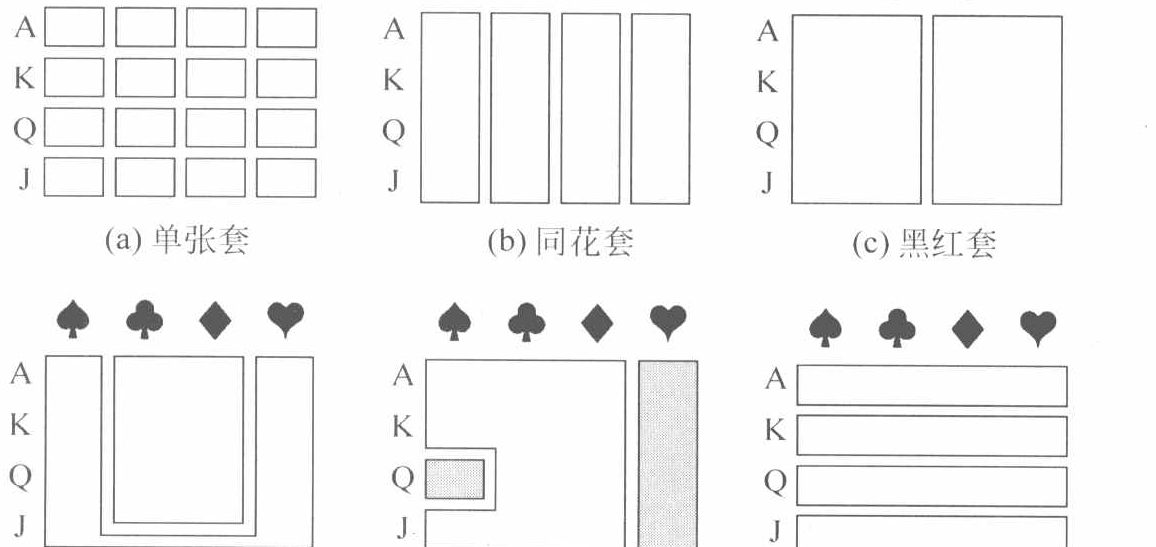
\includegraphics[width=97.8mm]{figs/fig_pg536_1.png}
\phantomsection\label{fig:12.1}\mvcap{图 12.1\quad 纸牌分组}
\end{mvfigure}

在聚类分析的大多数实际应用中, 研究者清楚了解如何区分“好”的分组与“坏”的分组. 那么为什么不列出有可能的分组, 然后从中选择“最优”分组, 以供未来研究?

%% ===== pg-537 =====

% ---- pg-537 （书页 525） ----

在扑克牌的例子中, 将 16 张牌分为一组有一种方法. 有 32 767 种方法将 16 张牌分为两组(各组牌的张数可以不同). 有 7 141 686 种方法将牌分为三组(各组牌的张数可以不同), 等等.\footnote{将 $n$ 个对象分成 $k$ 个非空组的方法数即第二类的斯特林(Stirling)数, 其值为 $(1/k!)\sum_{j=0}^{k}(-1)^{k-j}\binom{k}{j}j^{n}$ (见文献[1]). 将这些数对 $k=1,2,\cdots,n$ 求和, 就得出将 $n$ 个对象分组的所有可能的方法数.} 显然, 由于时间的限制, 要从所有可能的分组中找出最优分组是不可能的. 即使大型计算机也难以处理这么多的计算量. 因此必须建立一些\mvbold{算法}, 利用它们可以找到好的, 但未必是最好的分组.

总之, 聚类分析的基本目标是发现项目(或变量)的自然分组方法. 为此, 我们必须先建立一个定量尺度, 借以量度对象之间的联系(相似性). 12.2 节用来讨论各种相似性量度. 在该节之后, 我们介绍几种比较通用的将对象分组的算法.

即使没有关于自然分组的确切概念, 我们也经常能凭眼睛将二维或三维图中的对象进行分组. 1.4 节中讨论过的星图和切尔诺夫脸可用于此种目的(见例 1.11 和 1.12). 还有一些方法能将高维观测值描绘为二维空间中的点, 因而从某种意义上说可使相似的对象彼此更接近. 这些方法将在 12.5$\sim$12.7 节中加以考虑.

\section{相似性量度}
\phantomsection\label{sec:12.2}

为了从复杂的数据集产生出比较简单的组结构, 多数做法都要求有一个“接近程度”或“相似性”的量度. 在选择相似性量度时, 通常会掺入相当大的主观性. 需要考虑的重要问题包括变量的性质(离散型、连续型、二值型), 测量值的尺度(名目尺度、顺序尺度、间隔尺度、比例尺度), 以及关于研究课题的知识.

当一些项目(单元或事例)被聚类时, 它们之间的接近程度通常用某种距离来表示. 另一方面, 变量通常根据相关系数或类似的联系量度来分组.

\mvsub{项目对的距离与相似性系数}

我们在第 1 章的 1.5 节曾讨论过距离概念. 根据\hyperref[eq:1-12]{式(1-12)}, 两个 $p$ 维观测值(项目) $\mathbf{x}=[x_1,\cdots,x_p]'$ 和 $\mathbf{y}=[y_1,\cdots,y_p]'$ 之间的欧氏距离(直线距离)为
\phantomsection\label{eq:12-1}
\begin{equation}
\begin{aligned}
d(\mathbf{x},\mathbf{y})&=\sqrt{(x_1-y_1)^2+(x_2-y_2)^2+\cdots+(x_p-y_p)^2}\\
&=\sqrt{(\mathbf{x}-\mathbf{y})'(\mathbf{x}-\mathbf{y})}
\end{aligned}
\tag{12-1}
\end{equation}
而同样两个观测值之间的统计距离[见\hyperref[eq:1-23]{式(1-23)}]为
\phantomsection\label{eq:12-2}
\begin{equation}
d(\mathbf{x},\mathbf{y})=\sqrt{(\mathbf{x}-\mathbf{y})'\mathbf{A}(\mathbf{x}-\mathbf{y})}
\tag{12-2}
\end{equation}
通常 $\mathbf{A}=\mathbf{S}^{-1}$, 其中 $\mathbf{S}$ 为样本方差和协方差矩阵. 但是, 没有关于不同组的先验知识, 这些样本量就无法计算. 由于这个原因, 在聚类问题中更倾向于采用欧氏距离.

另一种距离量度是闵可夫斯基(Minkowski)度量
\phantomsection\label{eq:12-3}
\begin{equation}
d(\mathbf{x},\mathbf{y})=\left[\sum_{i=1}^{p}|x_i-y_i|^{m}\right]^{1/m}
\tag{12-3}
\end{equation}
对 $m=1$, $d(\mathbf{x},\mathbf{y})$ 所量度的是 $p$ 维空间两个点之间的“城市街区”距离. 对 $m=2$, $d(\mathbf{x},\mathbf{y})$ 就是欧氏距离. 一般说来, 改变 $m$ 就改变了赋予较大或较小差值的权值.

两个额外的关于“距离”或相异性的常用量度为坎贝拉(Canberra)度量和捷卡诺夫斯基(Czekanowski)系数. 这两个量度都只对非负变量定义. 我们有

%% ===== pg-538 =====

% ---- pg-538 （书页 526） ----

\phantomsection\label{eq:12-4}
\begin{equation}
\text{坎贝拉度量:}\quad d(\mathbf{x},\mathbf{y})=\sum_{i=1}^{p}\frac{|x_i-y_i|}{(x_i+y_i)}
\tag{12-4}
\end{equation}

\phantomsection\label{eq:12-5}
\begin{equation}
\text{捷卡诺夫斯基度量:}\quad d(\mathbf{x},\mathbf{y})=1-\frac{2\sum\limits_{i=1}^{p}\min(x_i,y_i)}{\sum\limits_{i=1}^{p}(x_i+y_i)}
\tag{12-5}
\end{equation}

只要有可能, 我们就建议采用“真实”距离[即满足\hyperref[eq:1-25]{式(1-25)}中的距离性质的距离]来聚类对象. 另一方面, 大多数聚类算法将接受主观指定的距离数, 它们可能不满足, 比如说三角不等式.

下面的例子说明怎样通过将距离矩阵的元素简单地进行重新组织就能完成初步分类.

当项目不能由有意义的 $p$ 维度量来表示时, 常根据某些特征的存在与否将各项目对进行比较. 相似项目比不相似项目有更多的共同特征. 一个特征是否存在, 可以从数学上引进一个二值变量来表示, 当特征存在时令这个变量取值 1, 特征不存在时则令它取值 0. 举例说, 对于有 $p=5$ 个二值变量的情形, 两个项目 $i$ 与 $k$ 的“得分”可能出现如下组合:

\begin{mvtable}
\begin{tabular}{l|ccccc}
\toprule
 & \multicolumn{5}{c}{变\quad 量}\\
\cmidrule(lr){2-6}
 & 1 & 2 & 3 & 4 & 5\\
\midrule
项目 $i$ & 1 & 0 & 0 & 1 & 1\\
项目 $k$ & 1 & 1 & 0 & 1 & 0\\
\bottomrule
\end{tabular}
\end{mvtable}

在这种情况下, 有两个 1—1 配对, 1 个 0—0 配对, 以及两个错配(0—1 和 1—0).

设 $x_{ij}$ 为第 $j$ 个二值变量在第 $i$ 个项目上的得分(1 或 0), $x_{kj}$ 为第 $j$ 个变量在第 $k$ 个项目上的得分(同样是 1 或 0), $j=1,2,\cdots,p$. 因此
\phantomsection\label{eq:12-6}
\begin{equation}
(x_{ij}-x_{kj})^2=\begin{cases}
0 & \text{若 } x_{ij}=x_{kj}=1 \text{ 或 } x_{ij}=x_{kj}=0\\
1 & \text{若 } x_{ij}\neq x_{kj}
\end{cases}
\tag{12-6}
\end{equation}
故欧氏距离平方 $\sum\limits_{j=1}^{p}(x_{ij}-x_{kj})^2$ 为错配的个数. 大距离对应有许多错配的情形, 也就是说与相异项目相对应. 对前面所举的例子, 项目 $i$ 与 $k$ 之间的距离平方为
\[
\begin{aligned}
\sum_{j=1}^{p}(x_{ij}-x_{kj})^2&=(1-1)^2+(0-1)^2+(0-0)^2+(1-1)^2+(1-0)^2\\
&=2
\end{aligned}
\]
虽然基于\hyperref[eq:12-6]{式(12-6)}的距离可用来量度相似性, 它却为 1—1 配对与 0—0 配对提供相同的权. 然而在某些情形下, 1—1 配对是比 0—0 更强的相似性指标. 例如, 在人的分组中, 两个人都能阅读古希腊文同两人都没有这种能力相比是一种更强的相似性证据. 因此, 将 0—0 配对降权甚至完全不予考虑, 也许是一种合理的做法. 为允许对 1—1 配对和 0—0 配对有不同处理, 曾提出过几种定义相似性系数的方案.

为了引进这些方案, 让我们将项目 $i$ 和 $k$ 的配对与错配的频数以列联表的形式列出:

\phantomsection\label{eq:12-7}
\begin{equation}
\begin{array}{ll|cc|c}
\hline
 & & \multicolumn{2}{c|}{项目 $k$} & \\
\cline{3-4}
 & & 1 & 0 & 合\quad 计\\
\hline
项目 $i$ & 1 & $a$ & $b$ & $a+b$\\
 & 0 & $c$ & $d$ & $c+d$\\
\hline
合\quad 计 & & $a+c$ & $b+d$ & $p=a+b+c+d$\\
\hline
\end{array}
\tag{12-7}
\end{equation}

%% ===== pg-539 =====

% ---- pg-539 （书页 527） ----

表中的 $a$ 为 1—1 配对频数, $b$ 为 1—0 配对频数, 等等. 对前面给出的五对二值变量来说, $a=2$, 而 $b=c=d=1$.

\hyperref[tab:12.1]{表 12.1} 列出一些用\hyperref[eq:12-7]{式(12-7)}中的频数定义的常用相似性系数. 每个定义之后附有对该定义基本依据的简短说明.

\begin{mvtable}
\phantomsection\label{tab:12.1}\mvtabcap{表 12.1\quad 聚类项目的相似性系数(对 $p$ 个二值变量)}
\begin{tabular}{ll}
\toprule
系\quad 数 & 基本依据说明\\
\midrule
1.\quad $\dfrac{a+d}{p}$ & 对 1—1 和 0—0 配对有相同的权.\\
2.\quad $\dfrac{2(a+d)}{2(a+d)+b+c}$ & 对 1—1 和 0—0 配对有加倍的权.\\
3.\quad $\dfrac{a+d}{a+d+2(b+c)}$ & 对不相配的对有加倍的权.\\
4.\quad $\dfrac{a}{p}$ & 分子中无 0—0 配对.\\
5.\quad $\dfrac{a}{a+b+c}$ & 分子分母中均无 0—0 配对.\\
  & (0—0 配对作为无关配对处理.)\\
6.\quad $\dfrac{2a}{2a+b+c}$ & 分子分母中均无 0—0 配对.\\
  & 对 1—1 配对有加倍的权.\\
7.\quad $\dfrac{a}{a+2(b+c)}$ & 分子分母中均无 0—0 配对.\\
  & 对不相配的对有加倍的权.\\
8.\quad $\dfrac{a}{b+c}$ & 除去 0—0 配对后, 1—1 配对与错配之比.\\
\bottomrule
\end{tabular}
\end{mvtable}

表中系数 1, 2 和 3 是单调关联的. 假定系数 1 是对表 I 和表 II 两个列联表计算的. 此时若 $(a_{\mathrm{I}}+d_{\mathrm{I}})/p\ge(a_{\mathrm{II}}+d_{\mathrm{II}})/p$, 我们也有 $2(a_{\mathrm{I}}+d_{\mathrm{I}})/[2(a_{\mathrm{I}}+d_{\mathrm{I}})+b_{\mathrm{I}}+c_{\mathrm{I}}]\ge 2(a_{\mathrm{II}}+d_{\mathrm{II}})/[2(a_{\mathrm{II}}+d_{\mathrm{II}})+b_{\mathrm{II}}+c_{\mathrm{II}}]$. 系数 3 对表 I 的值也不会小于对表 II 的值(见练习 12.4). 系数 5, 6 和 7 也都保持它们的相对的顺序.

单调性是重要的, 因为当相似性的定义改变而相似性的相对顺序保持不变时, 某些聚类方法不受影响. 在 12.3 节中讨论的单联结和完全联结分层方法也不受影响. 对这些方法, 选择\hyperref[tab:12.1]{表 12.1} 中系数 1, 2 或 3 中的任一个都会产生相同的分组. 类似的, 选择系数 5, 6 或 7 中的任一个也产生相同的分组.

\noindent\textbf{例 12.1}\quad (计算相似性系数的值)

假定五个人具有以下特征:

\begin{mvtable}
\begin{tabular}{ccccccc}
\toprule
个人 & 身高(英寸) & 体重(磅) & 眼球颜色 & 头发颜色 & 优势手 & 性别\\
\midrule
1 & 68 & 140 & 绿 & 金 & 右 & 女\\
2 & 73 & 185 & 棕 & 黑 & 右 & 男\\
3 & 67 & 165 & 蓝 & 金 & 右 & 男\\
4 & 64 & 120 & 棕 & 黑 & 右 & 女\\
5 & 76 & 210 & 棕 & 黑 & 左 & 男\\
\bottomrule
\end{tabular}
\end{mvtable}

定义 6 个二值变量:
\[
X_1=\begin{cases}
1, & \text{身高}\ge 72 \text{ 英寸}\\
0, & \text{身高}<72 \text{ 英寸}
\end{cases}
\qquad
X_2=\begin{cases}
1, & \text{体重}\ge 150 \text{ 磅}\\
0, & \text{体重}<150 \text{ 磅}
\end{cases}
\]

%% ===== pg-540 =====

% ---- pg-540 （书页 528） ----

\[
X_3=\begin{cases}
1, & \text{棕色眼睛}\\
0, & \text{其他}
\end{cases}
\qquad
X_4=\begin{cases}
1, & \text{金色头发}\\
0, & \text{其他}
\end{cases}
\]

\[
X_5=\begin{cases}
1, & \text{右手优势}\\
0, & \text{左手优势}
\end{cases}
\qquad
X_6=\begin{cases}
1, & \text{女性}\\
0, & \text{男性}
\end{cases}
\]

个人 1 和个人 2 在 $p=6$ 个二值变量上的得分为

\begin{mvtable}
\begin{tabular}{c|cccccc}
\toprule
个人 & $\mathbf{X}_1$ & $\mathbf{X}_2$ & $\mathbf{X}_3$ & $\mathbf{X}_4$ & $\mathbf{X}_5$ & $\mathbf{X}_6$\\
\midrule
1 & 0 & 0 & 0 & 1 & 1 & 1\\
2 & 1 & 1 & 1 & 0 & 1 & 0\\
\bottomrule
\end{tabular}
\end{mvtable}

配对与错配的数目由下面的双向表给出.

\begin{mvtable}
\begin{tabular}{ll|cc|c}
\toprule
 & & \multicolumn{2}{c|}{个人 2} & \\
\cmidrule(lr){3-4}
 & & 1 & 0 & 合\quad 计\\
\midrule
个人 1 & 1 & 1 & 2 & 3\\
 & 0 & 3 & 0 & 3\\
\midrule
合\quad 计 & & 4 & 2 & 6\\
\bottomrule
\end{tabular}
\end{mvtable}

用给出等权配对的相似系数 1, 得到
\[
\frac{a+d}{p}=\frac{1+0}{6}=\frac{1}{6}
\]
继续用相似系数 1, 便可得到其余各对个人之间的相似性数字, 这些数字列于下面的 $5\times 5$ 对称矩阵中.

\[
\begin{array}{r@{\;}c}
 & \begin{array}{ccccc}1&2&3&4&5\end{array}\\[2pt]
\begin{array}{r}1\\2\\3\\4\\5\end{array} &
\left[\begin{array}{ccccc}
1&&&&\\
\frac{1}{6}&1&&&\\
\frac{4}{6}&\frac{3}{6}&1&&\\
\frac{4}{6}&\frac{3}{6}&\frac{2}{6}&1&\\
0&\tikz{\node[draw,ellipse,inner sep=1pt]{$\frac{5}{6}$};}&\frac{2}{6}&\frac{2}{6}&1
\end{array}\right]
\end{array}
\]

根据相似系数的大小, 可以断言第二人与第五人最相似, 而第一人与第五人最不相似. 其余各对处于这两个极端之间. 如果我们根据相似性数字将这五个人分成相对接近的两组, 则可得出(1 3 4)和(2 5).

注意, $X_3=0$ 意味着眼球颜色不是棕色的, 故因此一个有蓝眼睛的人与一个有绿眼睛的人组成一个数 0—0 配对. 因此, 用相似性系数 1, 2 或 3 可能不合适, 因为这些系数对 1—1 配对和 0—0 配对赋予相等的权.\hfill$\blacksquare$

我们描述了距离和相似性的构造. 由距离来构造相似性总是可能的. 例如, 我们可以令
\phantomsection\label{eq:12-8}
\begin{equation}
\tilde{s}_{ik}=\frac{1}{1+d_{ik}}
\tag{12-8}
\end{equation}

%% ===== pg-541 =====

% ---- pg-541 （书页 529） ----

其中 $0<\tilde{s}_{ik}\le 1$ 为第 $i$ 个项目与第 $k$ 个项目之间的相似性, 而 $d_{ik}$ 则为相应的距离.

然而距离必须满足\hyperref[eq:1-25]{式(1-25)}, 所以不是总能由相似性来构造的. 正如高尔(Gower)所证明的那样(见文献[11]和[12]), 仅当相似性矩阵为非负定时才能做到这点. 在非负定条件下以及当最大相似性尺度已标准化(即 $\tilde{s}_{ii}=1$)时, 可以定义
\phantomsection\label{eq:12-9}
\begin{equation}
d_{ik}=\sqrt{2(1-\tilde{s}_{ik})}
\tag{12-9}
\end{equation}
且 $d_{ik}$ 满足距离的性质.

\mvsub{变量对的相似性及关联性量度}

迄今我们一直在对项目讨论相似性量度. 但在某些应用中, 必须进行分组的是变量而不是项目. 变量之间的相似性量度常取样本相关系数的形式. 不仅如此, 在某些聚类应用中, 负相关系数要用它们的绝对值来代替.

当变量为二值变量时, 又可将数据表示为列联表的形式. 不过这一次描述类别的是变量, 而不是项目. 对每一对变量, 有 $n$ 个项目被交叉分类成一个表. 对于通常的 0—1 代码, 此表具有如下形式:

\phantomsection\label{eq:12-10}
\begin{equation}
\begin{array}{ll|cc|c}
\hline
 & & \multicolumn{2}{c|}{变量 $k$} & \\
\cline{3-4}
 & & 1 & 0 & 合\quad 计\\
\hline
变量 $i$ & 1 & $a$ & $b$ & $a+b$\\
 & 0 & $c$ & $d$ & $c+d$\\
\hline
合\quad 计 & & $a+c$ & $b+d$ & $n=a+b+c+d$\\
\hline
\end{array}
\tag{12-10}
\end{equation}

例如, 在 $n$ 个项目中, 变量 $i=1$ 和变量 $k=0$ 的项目有 $b$ 个.

将通常的积矩相关系数公式用于列联表(12-10)中的二值变量, 就得到(见练习 12.3)
\phantomsection\label{eq:12-11}
\begin{equation}
r=\frac{ad-bc}{[(a+b)(c+d)(a+c)(b+d)]^{1/2}}
\tag{12-11}
\end{equation}
这个数可作为两个变量之间相似性的量度.

\hyperref[eq:12-11]{式(12-11)}中的相关系数与检验两个类别变量独立性的 $\chi^2$ 统计量有关($r=\chi^2/n$). 对给定的 $n$, 大的相似性(或相关性)与独立性不足相一致.

给定(12-10)中的表, 便可得出与\hyperref[tab:12.1]{表 12.1} 中所列内容完全类似的关联性(或相似性)量度. 唯一要做的改变是用 $n$(项目数)来代替 $p$(变量数).

\mvsub{相似性问题的小结}

为了对本节进行总结, 我们注意到有很多种方法可用来测量各对对象之间的相似性. 看来, 大多数实际工作者用距离[见\hyperref[eq:12-1]{式(12-1)}到\hyperref[eq:12-5]{式(12-5)}]或\hyperref[tab:12.2]{表 12.2} 中的相似性系数来对项目进行聚类, 而用相关系数对变量进行聚类. 然而, 有时输入聚类算法程序的也许仅仅是简单的频数.

\noindent\textbf{例 12.2}\quad (测量 11 种语言的相似性)

词的含义随着历史进程而变化. 然而数字 $1,2,3,\cdots$ 的意义却代表一个显而易见的例外. 这样, 语言的第一次比较也许可以用数词作比较对象. \hyperref[tab:12.2]{表 12.2} 给出英语、波兰语、匈牙利语及其他八种现代欧洲语言的前 10 个数字. (只考虑使用罗马字母的语言, 而且重音符、变音符、分音符等均予省略.) 对表中数词的拼法作粗略考察后便可发现, 前 5 种语言(英语、挪威语、

%% ===== pg-542 =====

% ---- pg-542 （书页 530） ----

丹麦语、荷兰语和德语)非常相似. 法语、西班牙语和意大利语彼此更为接近. 匈牙利语和芬兰语看来自成一家, 而波兰语则具有每一个较大语言组的某些特征.

\begin{mvtable}
\phantomsection\label{tab:12.2}\mvtabcap{表 12.2\quad 11 种语言中的数词}
\footnotesize
\begin{tabular}{ccccccccccc}
\toprule
英语 & 挪威语 & 丹麦语 & 荷兰语 & 德语 & 法语 & 西班牙语 & 意大利语 & 波兰语 & 匈牙利语 & 芬兰语\\
(E) & (N) & (Da) & (Du) & (G) & (Fr) & (Sp) & (I) & (P) & (H) & (Fi)\\
\midrule
one & en & en & een & eins & un & uno & uno & jeden & egy & yksi\\
two & to & to & twee & zwei & deux & dos & due & dwa & ketto & kaksi\\
three & tre & tre & drie & drei & trois & tres & tre & trzy & harom & kolme\\
four & fire & fire & vier & vier & quatre & cuatro & quattro & cztery & negy & neljä\\
five & fem & fem & vijf & funf & cinq & cinco & cinque & piec & ot & viisi\\
six & seks & seks & zes & sechs & six & seis & sei & szesc & hat & kuusi\\
seven & sju & syv & zeven & sieben & sept & siete & sette & siedem & het & seitseman\\
eight & atte & otte & acht & acht & huit & ocho & otto & osiem & nyolc & kahdeksan\\
nine & ni & ni & negen & neun & neuf & nueve & nove & dziewiec & kilenc & yhdeksan\\
ten & ti & ti & tien & zehn & dix & diez & dieci & dziesiec & tiz & kymmenen\\
\bottomrule
\end{tabular}
\end{mvtable}

在法语、西班牙语和意大利语中, 1 这个词全都由字母 u 开头. 为达到说明的目的, 我们可以用考察这些数词第一个字母的办法来比较这几种语言. 如果这两个词的首字母相同, 我们就说两种语言中表达同一个数字的词是和谐的; 否则就说它们是不和谐的. \hyperref[tab:12.2]{表 12.2} 中数字 $1\sim 10$ 的和谐表(首字母配对的频数表)由\hyperref[tab:12.3]{表 12.3} 给出. 我们看到, 英语和挪威语的 10 对词中有 8 对的首字母相同. 其余频数可用同样的方法计算.

\begin{mvtable}
\phantomsection\label{tab:12.3}\mvtabcap{表 12.3\quad 11 种语言中数词的首字母配对频数}
\footnotesize
\begin{tabular}{cccccccccccc}
\toprule
 & E & N & Da & Du & G & Fr & Sp & I & P & H & Fi\\
\midrule
E & 10 & & & & & & & & & &\\
N & 8 & 10 & & & & & & & & &\\
Da & 8 & 9 & 10 & & & & & & & &\\
Du & 3 & 5 & 4 & 10 & & & & & & &\\
G & 4 & 6 & 5 & 5 & 10 & & & & & &\\
Fr & 4 & 4 & 4 & 1 & 3 & 10 & & & & &\\
Sp & 4 & 4 & 5 & 1 & 3 & 8 & 10 & & & &\\
I & 4 & 4 & 5 & 1 & 3 & 9 & 9 & 10 & & &\\
P & 3 & 3 & 4 & 0 & 2 & 5 & 7 & 6 & 10 & &\\
H & 1 & 2 & 2 & 2 & 1 & 0 & 0 & 0 & 0 & 10 &\\
Fi & 1 & 1 & 1 & 1 & 1 & 1 & 1 & 1 & 1 & 2 & 10\\
\bottomrule
\end{tabular}
\end{mvtable}

\hyperref[tab:12.3]{表 12.3} 中的结果进一步证实了我们从\hyperref[tab:12.2]{表 12.2} 中得到的最初直观印象. 也就是说, 英语、挪威语、丹麦语、荷兰语和德语看起来构成一组, 法语、西班牙语、意大利语和波兰语也可以分在同一组, 而匈牙利语和芬兰语则各自成为单独的一组.\hfill$\blacksquare$

到目前为止所举的例子中, 都是根据我们对相似性或距离量度的直观印象来分组的. 现在我们来讨论较少主观性的聚类方案.

%% ===== pg-543 =====

% ---- pg-543 （书页 531） ----

\section{分层聚类方法}
\phantomsection\label{sec:12.3}

即使使用最大最快的计算机, 我们也几乎不可能考察所有可能的分组情况. 由于这个原因, 人们提出各种各样的聚类算法, 以期能找到“合理”的聚类而又不必考察所有可能的结构.

分层聚类方法是通过一系列或者是相继的合并, 或者是相继的分割来进行的. 聚集分层法从单个对象开始. 这样在开始时有多个对象就有多少个聚类. 将那些最相似的对象首先分组, 然后将组与组根据它们之间的相似性进行合并. 最后随着相似性不断下降, 所有的组渐渐融合为一个聚类.

分割分层法的工作方式与聚集分层法正相反. 最初由所有对象组成的一个组开始, 将它分割成两个子组, 使一个子组的对象“远离”另一子组的对象. 然后将这两个组进一步分割成不相似的组. 这一过程一直到每个对象单独成为一组时为止.

聚集和分割这两种方法的结果可以用二维空间的图来表示, 这种图称为“树图”. 我们将看到, 用树图可以说明相继完成的历次合并或分割.

在本节中, 我们将集中讨论聚集分层方法, 特别是连接法. 在文献[3]和[8]中可找到关于分割分层法和其他聚集分层法的出色的初步介绍.

连接法既适用于对项目的聚类, 也适用于对变量的聚类. 不过这种情况并非对所有聚集分层法都成立. 我们将依次讨论单连接(最小距离或最近邻点)、完全连接(最大距离或最远邻点), 以及平均连接(平均距离). \hyperref[fig:12.2]{图 12.2} 是在这三种连接准则下聚类合并的示意图.

\begin{mvfigure}
\begin{tikzpicture}[every node/.style={outer sep=1pt}]
% ---------------- (a) ----------------
\begin{scope}
\draw[dashed] (0,0) ellipse (1.15 and 0.85);
\draw[dashed] (3.0,0) ellipse (1.05 and 0.95);
\fill (-0.50,0.20) circle (1.6pt); \node[above left] at (-0.50,0.20) {1};
\fill (-0.45,-0.45) circle (1.6pt); \node[below left] at (-0.45,-0.45) {2};
\fill (3.25,0.55) circle (1.6pt); \node[above left] at (3.25,0.55) {3};
\fill (2.80,0.05) circle (1.6pt); \node[above left] at (2.80,0.05) {4};
\fill (3.40,-0.50) circle (1.6pt); \node[below left] at (3.40,-0.50) {5};
\draw (-0.45,-0.45) -- (2.80,0.05);
\node at (5.60,-0.05) {$\dfrac{\text{类间距离}}{d_{24}}$};
\node at (1.45,-1.80) {(a) 单连接};
\end{scope}
% ---------------- (b) ----------------
\begin{scope}[yshift=-3.5cm]
\draw[dashed] (0,0) ellipse (1.15 and 0.85);
\draw[dashed] (3.0,0) ellipse (1.05 and 0.95);
\fill (-0.50,0.20) circle (1.6pt); \node[above left] at (-0.50,0.20) {1};
\fill (-0.45,-0.45) circle (1.6pt); \node[below left] at (-0.45,-0.45) {2};
\fill (3.25,0.55) circle (1.6pt); \node[above left] at (3.25,0.55) {3};
\fill (2.80,0.05) circle (1.6pt); \node[above left] at (2.80,0.05) {4};
\fill (3.40,-0.50) circle (1.6pt); \node[below left] at (3.40,-0.50) {5};
\draw (-0.50,0.20) -- (3.40,-0.50);
\node at (5.60,-0.05) {$d_{15}$};
\node at (1.45,-1.80) {(b) 完全连接};
\end{scope}
% ---------------- (c) ----------------
\begin{scope}[yshift=-7.0cm]
\draw[dashed] (0,0) ellipse (1.15 and 0.85);
\draw[dashed] (3.0,0) ellipse (1.05 and 0.95);
\fill (-0.50,0.20) circle (1.6pt); \node[above left] at (-0.50,0.20) {1};
\fill (-0.45,-0.45) circle (1.6pt); \node[below left] at (-0.45,-0.45) {2};
\fill (3.25,0.55) circle (1.6pt); \node[above left] at (3.25,0.55) {3};
\fill (2.80,0.05) circle (1.6pt); \node[above left] at (2.80,0.05) {4};
\fill (3.40,-0.50) circle (1.6pt); \node[below left] at (3.40,-0.50) {5};
\draw (-0.50,0.20) -- (3.25,0.55);
\draw (-0.50,0.20) -- (2.80,0.05);
\draw (-0.50,0.20) -- (3.40,-0.50);
\draw (-0.45,-0.45) -- (3.25,0.55);
\draw (-0.45,-0.45) -- (2.80,0.05);
\draw (-0.45,-0.45) -- (3.40,-0.50);
\node at (6.10,-0.05) {$\dfrac{d_{13}+d_{14}+d_{15}+d_{23}+d_{24}+d_{25}}{6}$};
\node at (1.45,-1.80) {(c) 平均连接};
\end{scope}
\end{tikzpicture}
\phantomsection\label{fig:12.2}\mvcap{图 12.2\quad 类间距离(相异性)}
\end{mvfigure}

从图中可以看到, 当两个组根据它们最邻近成员之间的距离融合时, 便产生单连接结果; 当两个组根据它们最远成员之间的距离融合时, 便产生完全连接; 当两个组根据它们相应位置上的各对成员之间的平均距离融合时, 便产生平均连接.

下面是将 $N$ 个对象(项目或变量)分组时聚集分层聚类算法的操作步骤:

1.\quad 从 $N$ 个类(每类只含一个元素)和 $N\times N$ 对称距离(或相似性)矩阵 $\mathbf{D}=\{d_{ik}\}$ 开始.

2.\quad 从距离阵中搜寻最邻近(最相似)的两个类. 记“最相似”的两个类为 $U$ 和 $V$, 它们之间的距离记为 $d_{UV}$.

%% ===== pg-544 =====

% ---- pg-544 （书页 532） ----

3.\quad 合并 $U$ 与 $V$, 将新的类记为 $(UV)$. 将矩阵 $\mathbf{D}$ 中的元素更新: (a)删除原来 $U$ 和 $V$ 所对应的行和列, (b)将给出类 $(UV)$ 与其余各类之间距离的行和列加进该矩阵.

4.\quad 将步骤 2 和 3 重复 $N-1$ 次(当算法结束时所有对象将在一个类中). 记录下被合并的各个类的一致性以及历次合并的水平(距离或相似性).\hfill(12-12)

隐藏在任 何聚类方法背后的思想, 都可以通过实例来表达. 我们对连接方法的输入和算法组成部分作一番简要讨论之后再介绍这些例子.

\mvsub{单连接法}

单连接算法的输入可以是对象对之间的距离或相似性. 各个组由个体通过合并最近邻近点而形成, 此处的最近邻近点可以指最小距离或最大相似性.

一开始我们必须找到 $\mathbf{D}=\{d_{ij}\}$ 中的最小距离, 并将相应的对象比如说 $U$ 和 $V$ 合并, 得到聚类 $(UV)$. 对一般算法(12-12)中的步骤 3, $(UV)$ 与任一其他聚类 $W$ 之间的距离为
\phantomsection\label{eq:12-13}
\begin{equation}
d_{(UV)W}=\min\{d_{UW},d_{VW}\}
\tag{12-13}
\end{equation}
这里 $d_{UW}$ 和 $d_{VW}$ 分别为聚类 $U$ 与 $W$ 及聚类 $V$ 与 $W$ 的最近邻近点之间的距离.

单连接聚类的结果可以用树图表示. 树的分枝代表聚类. 分枝在结点处汇合(合并), 而沿距离(或相似性)轴的各个结点位置指明合并发生时的水平(即距离或相似性的大小). 我们在下面几个例子中考虑某些特殊情形下的树图.

\noindent\textbf{例 12.3}\quad (用单连接法聚类)

为说明单连接算法, 我们考虑以下的五个对象之间的假想距离如下:
\[
\mathbf{D}=\{d_{ik}\}=
\begin{array}{r@{\;}c}
 & \begin{array}{ccccc}1&2&3&4&5\end{array}\\[2pt]
\begin{array}{r}1\\2\\3\\4\\5\end{array} &
\left[\begin{array}{ccccc}
0&&&&\\
9&0&&&\\
3&7&0&&\\
6&5&9&0&\\
11&10&\tikz{\node[draw,ellipse,inner sep=1pt]{2};}&8&0
\end{array}\right]
\end{array}
\]
将每个对象看成是一个类, 我们的聚类从合并两个最接近的项目开始. 由于
\[
\min_{i,k}(d_{ik})=d_{53}=2
\]
对象 5 和 3 合并, 形成聚类(35). 为确定下一个聚类水平, 我们需要得到聚类(35)与其余对象 1, 2, 4 之间的距离. 最近邻近点距离为
\[
\begin{aligned}
d_{(35)1}&=\min\{d_{31},d_{51}\}=\min\{3,11\}=3\\
d_{(35)2}&=\min\{d_{32},d_{52}\}=\min\{7,10\}=7\\
d_{(35)4}&=\min\{d_{34},d_{54}\}=\min\{9,8\}=8
\end{aligned}
\]
从 $\mathbf{D}$ 中将对应于对象 3 和 5 的行和列删除, 并将对应于(35)的行和列加上, 便得到新的距离阵
\[
\begin{array}{r@{\;}c}
 & \begin{array}{cccc}(35)&1&2&4\end{array}\\[2pt]
\begin{array}{r}(35)\\1\\2\\4\end{array} &
\left[\begin{array}{cccc}
0&&&\\
\tikz{\node[draw,ellipse,inner sep=1pt]{3};}&0&&\\
7&9&0&\\
8&6&5&0
\end{array}\right]
\end{array}
\]
在这个距离阵中, 各对聚类之间的最小距离为 $d_{(35)1}=3$, 于是我们将聚类(1)与聚类(35)合并, 得到下一个聚类(135). 算出

%% ===== pg-545 =====

% ---- pg-545 （书页 533） ----

\[
\begin{aligned}
d_{(135)2}&=\min\{d_{(35)2},d_{12}\}=\min\{7,9\}=7\\
d_{(135)4}&=\min\{d_{(35)4},d_{14}\}=\min\{8,6\}=6
\end{aligned}
\]
我们得到下一个聚类水平的距离矩阵为
\[
\begin{array}{r@{\;}c}
 & \begin{array}{ccc}(135)&2&4\end{array}\\[2pt]
\begin{array}{r}(135)\\2\\4\end{array} &
\left[\begin{array}{ccc}
0&&\\
7&0&\\
6&\tikz{\node[draw,ellipse,inner sep=1pt]{5};}&0
\end{array}\right]
\end{array}
\]
各对聚类之间的最小最近邻近点距离为 $d_{42}=5$, 于是我们将对象 4 和 2 合并, 得到聚类(24).

现在我们有两个不同的聚类(135)和(24). 它们的最邻近点距离(即唯一的距离)为
\[
d_{(135)(24)}=\min\{d_{(135)2},d_{(135)4}\}=\min\{7,6\}=6
\]
最终的距离阵变成
\[
\begin{array}{r@{\;}c}
 & \begin{array}{cc}(135)&(24)\end{array}\\[2pt]
\begin{array}{r}(135)\\(24)\end{array} &
\left[\begin{array}{cc}
0&\\
\tikz{\node[draw,ellipse,inner sep=1pt]{6};}&0
\end{array}\right]
\end{array}
\]
于是将聚类(135)和(24)合并, 形成一个包含全部五个对象的聚类(12345), 此时最近邻近点距离为 6.

图解上述分层聚类过程的树图示于\hyperref[fig:12.3]{图 12.3}. 此图清楚说明了分组与分组发生时的距离水平.\hfill$\blacksquare$

\begin{mvfigure}
\begin{tikzpicture}[x=1.0cm,y=0.42cm,every node/.style={font=\small}]
% 坐标轴
\draw (-0.5,0) -- (-0.5,6.5);
\foreach \ty in {0,1,2,3,4,5,6} { \draw (-0.5,\ty) -- (-0.62,\ty); }
\foreach \ty/\tl in {0/0, 2/2, 4/4, 6/6} { \node[left] at (-0.66,\ty) {\tl}; }
\node[rotate=90] at (-1.30,3) {距离};
\draw (-0.5,0) -- (4.45,0);
% 叶结点
\foreach \lx/\lab in {0/1, 1/3, 2/5, 3/2, 4/4} {
  \node[circle,fill,inner sep=1.4pt] at (\lx,0) {};
  \node[below] at (\lx,-0.30) {\lab};
}
\node at (2,-1.20) {对象};
% 树
\draw (1,0) -- (1,2); \draw (2,0) -- (2,2); \draw (1,2) -- (2,2);
\draw (1.5,2) -- (1.5,3);
\draw (0,0) -- (0,3); \draw (0,3) -- (1.5,3);
\draw (0.75,3) -- (0.75,6);
\draw (3,0) -- (3,5); \draw (4,0) -- (4,5); \draw (3,5) -- (4,5);
\draw (3.5,5) -- (3.5,6);
\draw (0.75,6) -- (3.5,6);
\end{tikzpicture}
\phantomsection\label{fig:12.3}\mvcap{图 12.3\quad 五个对象之间距离的单连接树图}
\end{mvfigure}

在典型的分层聚类应用中, 人们感兴趣的主要是中间结果, 即将对象分为中等数目的聚类.

\noindent\textbf{例 12.4}\quad (11 种语言的单连接聚类)

考虑\hyperref[tab:12.3]{表 12.3} 中的和谐矩阵, 它代表 11 种语言中前 10 个数字词之间的接近程度. 为构造距离矩阵, 我们将和谐性(两种语言的 10 个数字的首字母相同的频数)从完全一致的数 10(每种语言自身的固有频数)中减去, 得到的距离阵为

\begin{mvtable}
\footnotesize
\[
\begin{array}{r@{\;}c}
 & \begin{array}{ccccccccccc}\mathrm{E}&\mathrm{N}&\mathrm{Da}&\mathrm{Du}&\mathrm{G}&\mathrm{Fr}&\mathrm{Sp}&\mathrm{I}&\mathrm{P}&\mathrm{H}&\mathrm{Fi}\end{array}\\[2pt]
\begin{array}{r}\mathrm{E}\\\mathrm{N}\\\mathrm{Da}\\\mathrm{Du}\\\mathrm{G}\\\mathrm{Fr}\\\mathrm{Sp}\\\mathrm{I}\\\mathrm{P}\\\mathrm{H}\\\mathrm{Fi}\end{array} &
\left[\begin{array}{ccccccccccc}
0&&&&&&&&&&\\
2&0&&&&&&&&&\\
2&\tikz{\node[draw,ellipse,inner sep=1pt]{1};}&0&&&&&&&&\\
7&5&6&0&&&&&&&\\
6&4&5&5&0&&&&&&\\
6&6&6&9&7&0&&&&&\\
6&6&5&9&7&2&0&&&&\\
6&6&5&9&7&\tikz{\node[draw,ellipse,inner sep=1pt]{1};}&\tikz{\node[draw,ellipse,inner sep=1pt]{1};}&0&&&\\
7&7&6&10&8&5&3&4&0&&\\
9&8&8&8&9&10&10&10&10&0&\\
9&9&9&9&9&9&9&9&9&8&0
\end{array}\right]
\end{array}
\]
\end{mvtable}

%% ===== pg-546 =====

% ---- pg-546 （书页 534） ----

我们首先搜索各对语言(聚类)之间的最小距离. 最小距离 1 出现在丹麦语与挪威语, 意大利语与法语, 及意大利语与西班牙语之间. 将语言依出现在表中的顺序编号, 我们有
\[
d_{32}=1;\qquad d_{86}=1;\qquad d_{87}=1
\]
由于 $d_{76}=2$, 只能合并 8 和 6, 或者合并 8 和 7. 但不能在 1 的水平上将 6,7,8 三者合并. 我们选择先合并 6 和 8, 然后更新距离阵, 并合并 2 和 3, 得到聚类(68)和(23). 随后的计算机计算产生\hyperref[fig:12.4]{图 12.4} 中的树图.

\begin{mvfigure}
\begin{tikzpicture}[x=0.92cm,y=0.42cm,line width=0.5pt]

% ---------- 叶结点的竖线 ----------
\draw (0,0) -- (0,2.2);
\draw (1,0) -- (1,0.87);
\draw (2,0) -- (2,0.87);
\draw (3,0) -- (3,0.87);
\draw (4,0) -- (4,0.87);
\draw (5,0) -- (5,2.16);
\draw (6,0) -- (6,5.05);
\draw (7,0) -- (7,5.05);
\draw (8,0) -- (8,5.05);
\draw (9,0) -- (9,8.64);
\draw (10,0) -- (10,8.64);

% ---------- 合并的横线 ----------
\draw (1,0.87) -- (2,0.87);
\draw (3,0.87) -- (4,0.87);
\draw (0,2.2) -- (1.5,2.2);
\draw (3.5,2.16) -- (5,2.16);
\draw (4.25,5.05) -- (6,5.05);
\draw (7,5.05) -- (8,5.05);
\draw (0.75,7.65) -- (5.125,7.65);
\draw (9,8.64) -- (10,8.64);
\draw (2.94,9.78) -- (9.5,9.78);

% ---------- 各聚类向上的竖线 ----------
\draw (1.5,0.87) -- (1.5,2.2);
\draw (3.5,0.87) -- (3.5,2.16);
\draw (0.75,2.2) -- (0.75,7.65);
\draw (4.25,2.16) -- (4.25,5.05);
\draw (5.125,5.05) -- (5.125,7.65);
\draw (7.5,5.05) -- (7.5,9.78);
\draw (2.94,7.65) -- (2.94,9.78);
\draw (9.5,8.64) -- (9.5,9.78);

% ---------- 坐标轴 ----------
\draw (-0.85,0) -- (-0.85,10.4);
\foreach \t in {0,2,4,6,8,10}{%
  \draw (-0.85,\t) -- (-0.62,\t);%
  \node[left,font=\small] at (-0.95,\t) {\t};%
}
\node[rotate=90,font=\small] at (-1.75,5) {距离};
\node[font=\small] at (5,-2.1) {语言};

% ---------- 叶结点的圆点与标记 ----------
\foreach \i/\l in {0/E,1/N,2/Da,3/Fr,4/I,5/Sp,6/P,7/Du,8/G,9/H,10/Fi}{%
  \fill (\i,0) circle (0.055);%
  \node[below,font=\small,inner sep=1.5pt] at (\i,0) {\l};%
}

\end{tikzpicture}
\phantomsection\label{fig:12.4}\mvcap{图 12.4\quad 11 种语言中前 10 个数词之间距离的单连接树图}
\end{mvfigure}

由这个树图我们看到, 挪威语和丹麦语, 以及法语和意大利语在最小距离(最大相似)水平上形成聚类, 当所允许的距离增大时, 英语加入挪威语—丹麦语组, 而西班牙语则并入法语—意大利语组. 注意匈牙利语和芬兰语之间的相似性比它们与其他语言聚类之间的相似性更大. 然而这两个聚类(语言)要到最后邻近点之间的距离有了很大增加之后才能合并. 最后, 所有的语言聚类在最近邻近点距离的最大值 9 这个水平上合并成一个聚类. \hfill$\blacksquare$

由于单连接方法用聚类之间的最短连接来合并聚类, 所以这种方法不能识别分离得很差的聚类[见\hyperref[fig:12.5]{图 12.5}(a)]. 另一方面, 单连接法是最能描绘非椭球形聚类的少数方法之一. 单连接法有一种挑选长链状聚类的倾向, 称为\mvbold{链接倾向}[见\hyperref[fig:12.5]{图 12.5}(b)]. 当项目位于链的两端因而颇不相似时, 链接法有可能产生误导.

\begin{mvfigure}
\begin{tikzpicture}[x=1.05cm,y=0.52cm,line width=0.5pt]

% ============ 点云宏: cx, cy, a, b, 倾角 ============
\def\cloud#1#2#3#4#5{%
  \pgfmathsetmacro\cth{cos(#5)}%
  \pgfmathsetmacro\sth{sin(#5)}%
  \foreach \f in {0.35,0.65,0.92}{%
    \foreach \a in {0,30,...,330}{%
      \pgfmathsetmacro\px{#1 + \f*(#3*cos(\a)*\cth - #4*sin(\a)*\sth)}%
      \pgfmathsetmacro\py{#2 + \f*(#3*cos(\a)*\sth + #4*sin(\a)*\cth)}%
      \fill (\px,\py) circle (0.04);%
    }%
  }%
}

% ================= (a) =================
\begin{scope}[shift={(0,0)}]
\draw (0,0) -- (3.4,0);
\draw (0,0) -- (0,3.4);
\node[rotate=90,font=\small] at (-0.45,1.7) {变量2};
\node[font=\small] at (1.7,-0.42) {变量1};
\cloud{1.15}{2.15}{0.85}{0.50}{35}
\cloud{2.15}{1.05}{0.80}{0.50}{35}
\node[font=\small,anchor=west] at (2.35,2.15) {椭圆形结构};
\node[font=\small] at (1.7,-1.05) {(a) 单连接在接近重叠时产生混淆};
\end{scope}

% ================= (b) =================
\begin{scope}[shift={(4.6,0)}]
\draw (0,0) -- (3.4,0);
\draw (0,0) -- (0,3.4);
\node[rotate=90,font=\small] at (-0.45,1.7) {变量2};
\node[font=\small] at (1.7,-0.42) {变量1};
% 链状连接
\coordinate (A) at (0.55,2.35);
\coordinate (B) at (1.05,1.75);
\coordinate (C) at (1.70,1.30);
\coordinate (D) at (2.30,1.45);
\coordinate (E) at (2.75,1.95);
\coordinate (F) at (0.85,2.75);
\coordinate (G) at (2.05,2.40);
\coordinate (H) at (2.60,0.95);
\draw (A) -- (B) -- (C) -- (D) -- (E);
\draw (F) -- (B);
\draw (D) -- (G);
\draw (D) -- (H);
\foreach \p in {A,B,C,D,E,F,G,H}{ \fill (\p) circle (0.055); }
% 虚线轮廓
\draw[dashed,rounded corners=26pt] (0.30,2.05) -- (1.00,2.95) -- (2.30,2.72) -- (3.05,1.55) -- (2.45,0.68) -- (0.75,1.10) -- cycle;
\node[font=\small,anchor=west] at (1.35,2.55) {非椭圆形结构};
\node[font=\small] at (1.7,-1.05) {(b) 链接效应};
\end{scope}

\end{tikzpicture}
\phantomsection\label{fig:12.5}\mvcap{图 12.5\quad 单连接聚类}
\end{mvfigure}

通过单连接法形成的聚类, 在对原始的距离(或相似性)作保序变换后保持不变. 具体说, 在\hyperref[tab:12.1]{表 12.1} 中, 任一组相互之间有单调关系的相似系数会产生相同的聚类.

\subsection{完全连接法}

完全连接聚类方式与单连接聚类方式在许多方面都相同, 但有一个重要区别: 在每个阶段, 聚类之间的距离(相似性)由两个聚类中相距最远的两个元素之间的距离确定. 这样, 完全

%% ===== pg-547 =====

% ---- pg-547 （书页 535） ----

连接就能保证: 对一个聚类中的所有项目, 彼此间的距离均不超过某个最大距离(或最小相似性).

一般的聚集算法从找到 $\mathbf{D}=\{d_{ik}\}$ 中的最小元素开始, 并将 $U$ 和 $V$ 这样的相应对象合并, 得到新的聚类 $(UV)$. 对式(12-12)中一般算法的步骤 3, $(UV)$ 与任一其他聚类 $W$ 之间的距离定义为
\phantomsection\label{eq:12-14}
\begin{equation}
d_{(UV)W}=\max\{d_{UW},d_{VW}\}
\tag{12-14}
\end{equation}
这里 $d_{UW}$ 和 $d_{VW}$ 分别为 $U$ 与 $W$ 及 $V$ 与 $W$ 的相隔最远的成员之间的距离.

\noindent\textbf{例 12.5}\quad (用完全连接法聚类)

回到例 12.4 中引进的距离矩阵
\[
\mathbf{D}=\{d_{ik}\}=
\begin{array}{cc}
\begin{array}{c}\mbox{}\\1\\2\\3\\4\\5\end{array} &
\begin{array}{c}
\begin{array}{ccccc}1&2&3&4&5\end{array}\\[2pt]
\begin{bmatrix}
0& & & & \\
9&0& & & \\
3&7&0& & \\
6&5&9&0& \\
11&10&\textcircled{2}&8&0
\end{bmatrix}
\end{array}
\end{array}
\]

在第一阶段, 将对象 3 和 5 合并, 因为它们最相似. 这样就得到聚类(35). 在第二阶段, 我们计算
\[
\begin{aligned}
d_{(35)1}&=\max\{d_{31},d_{51}\}=\max\{3,11\}=11\\
d_{(35)2}&=\max\{d_{32},d_{52}\}=10\\
d_{(35)4}&=\max\{d_{34},d_{54}\}=9
\end{aligned}
\]
于是距离阵修正为
\[
\begin{array}{cc}
\begin{array}{c}\mbox{}\\(35)\\1\\2\\4\end{array} &
\begin{array}{c}
\begin{array}{cccc}(35)&1&2&4\end{array}\\[2pt]
\begin{bmatrix}
0& & & \\
11&0& & \\
10&9&0& \\
9&6&\textcircled{5}&0
\end{bmatrix}
\end{array}
\end{array}
\]

下一次合并发生在两个最相似的组 2 与 4 之间, 得到一个新的聚类(24). 在第三阶段我们有
\[
\begin{aligned}
d_{(24)(35)}&=\max\{d_{2(35)},d_{4(35)}\}=\max\{10,9\}=10\\
d_{(24)1}&=\max\{d_{21},d_{41}\}=9
\end{aligned}
\]
因而距离阵为
\[
\begin{array}{cc}
\begin{array}{c}\mbox{}\\(35)\\(24)\\1\end{array} &
\begin{array}{c}
\begin{array}{ccc}(35)&(24)&1\end{array}\\[2pt]
\begin{bmatrix}
0& & \\
10&0& \\
11&\textcircled{9}&0
\end{bmatrix}
\end{array}
\end{array}
\]

\begin{mvfigure}
\begin{tikzpicture}[x=1.05cm,y=0.34cm,line width=0.5pt]
% 叶结点竖线
\draw (0,0) -- (0,11);
\draw (1,0) -- (1,5);
\draw (2,0) -- (2,5);
\draw (3,0) -- (3,2);
\draw (4,0) -- (4,2);
% 合并横线
\draw (1,5) -- (2,5);
\draw (3,2) -- (4,2);
\draw (1.5,9) -- (3.5,9);
\draw (0,11) -- (2.5,11);
% 向上的竖线
\draw (1.5,5) -- (1.5,9);
\draw (3.5,2) -- (3.5,9);
\draw (2.5,9) -- (2.5,11);
% 坐标轴
\draw (-0.75,0) -- (-0.75,12.3);
\foreach \t in {0,2,4,6,8,10,12}{%
  \draw (-0.75,\t) -- (-0.55,\t);%
  \node[left,font=\small] at (-0.85,\t) {\t};%
}
\node[rotate=90,font=\small] at (-1.7,6) {距离};
\node[font=\small] at (2,-2.6) {对象};
% 叶结点
\foreach \i/\l in {0/1,1/2,2/4,3/3,4/5}{%
  \fill (\i,0) circle (0.055);%
  \node[below,font=\small,inner sep=1.5pt] at (\i,0) {\l};%
}
\end{tikzpicture}
\phantomsection\label{fig:12.6}\mvcap{图 12.6\quad 五个对象之间距离的完全连接树图}
\end{mvfigure}

下一次合并产生聚类(124). 在最后阶段, 将组(35)和(124)合并成一个聚类(12345), 其距离水平为
\[
d_{(124)(35)}=\max\{d_{1(35)},d_{(24)(35)}\}=\max\{11,10\}=11
\]
这个聚类过程的树图由\hyperref[fig:12.6]{图 12.6} 给出. \hfill$\blacksquare$

比较\hyperref[fig:12.3]{图 12.3} 和\hyperref[fig:12.6]{图 12.6} 可以看出, 单连接法与完全连接法在将对象 1 分配给前面的组时分配方法是不一样的.

%% ===== pg-548 =====

% ---- pg-548 （书页 536） ----

\noindent\textbf{例 12.6}\quad (11 种语言的完全连接聚类)

在例 12.4 中我们给出了 11 种语言的距离阵. 将完全连接聚类算法应用于这个距离阵, 得出的树图见\hyperref[fig:12.7]{图 12.7}.

比较\hyperref[fig:12.7]{图 12.7} 和\hyperref[fig:12.4]{图 12.4}, 我们看到两种分层聚类法都产生出英语—挪威语—丹麦语组和法语—意大利语—西班牙语组. 在中间水平上, 波兰语被合并到法语—意大利语—西班牙语组. 此外, 两种方法都在倒数第二步才将匈牙利语和芬兰语合成一组.

\begin{mvfigure}
\begin{tikzpicture}[x=0.92cm,y=0.42cm,line width=0.5pt]

% ---------- 叶结点的竖线 ----------
\draw (0,0) -- (0,1.91);
\draw (1,0) -- (1,0.86);
\draw (2,0) -- (2,0.86);
\draw (3,0) -- (3,5.93);
\draw (4,0) -- (4,0.86);
\draw (5,0) -- (5,0.86);
\draw (6,0) -- (6,1.91);
\draw (7,0) -- (7,4.91);
\draw (8,0) -- (8,6.86);
\draw (9,0) -- (9,8.07);
\draw (10,0) -- (10,8.07);

% ---------- 合并的横线 ----------
\draw (1,0.86) -- (2,0.86);
\draw (4,0.86) -- (5,0.86);
\draw (0,1.91) -- (1.5,1.91);
\draw (4.5,1.91) -- (6,1.91);
\draw (5.25,4.91) -- (7,4.91);
\draw (0.75,5.93) -- (3,5.93);
\draw (1.875,6.86) -- (8,6.86);
\draw (9,8.07) -- (10,8.07);
\draw (4,9.02) -- (9.5,9.02);

% ---------- 各聚类向上的竖线 ----------
\draw (1.5,0.86) -- (1.5,1.91);
\draw (0.75,1.91) -- (0.75,5.93);
\draw (4.5,0.86) -- (4.5,1.91);
\draw (5.25,1.91) -- (5.25,4.91);
\draw (6.125,4.91) -- (6.125,6.86);
\draw (1.875,5.93) -- (1.875,6.86);
\draw (4,6.86) -- (4,9.02);
\draw (9.5,8.07) -- (9.5,9.02);

% ---------- 坐标轴 ----------
\draw (-0.85,0) -- (-0.85,10.3);
\foreach \t in {0,2,4,6,8,10}{%
  \draw (-0.85,\t) -- (-0.62,\t);%
  \node[left,font=\small] at (-0.95,\t) {\t};%
}
\node[rotate=90,font=\small] at (-1.75,5) {距离};
\node[font=\small] at (5,-2.1) {语言};

% ---------- 叶结点的圆点与标记 ----------
\foreach \i/\l in {0/E,1/N,2/Da,3/G,4/Fr,5/I,6/Sp,7/P,8/Du,9/H,10/Fi}{%
  \fill (\i,0) circle (0.055);%
  \node[below,font=\small,inner sep=1.5pt] at (\i,0) {\l};%
}

\end{tikzpicture}
\phantomsection\label{fig:12.7}\mvcap{图 12.7\quad 11 种语言中前 10 个数词之间距离的完全连接树图}
\end{mvfigure}

然而, 两种方法处理德语和荷兰语的结果不同. 单连接法在中等距离上将德语与荷兰语合并, 而且它们在最后的大合并之前始终是一个单独的聚类. 完全连接法在中间水平上将德语并入英语—挪威语—丹麦语组. 荷兰语保持为单独一组, 直到在较高的距离水平上才与英语—挪威语—丹麦语—德语组及法语—意大利语—西班牙语—波兰语组合并成一组. 完全连接的最终合并涉及两个聚类, 而单连接的最终合并涉及三个聚类. \hfill$\blacksquare$

\medskip
\noindent\textbf{例 12.7}\quad (用完全连接法对变量进行聚类)

从 22 家美国公用事业公司搜集到的 1975 年的数据列于\hyperref[tab:12.4]{表 12.4}. 虽然将公司进行聚类更令人感兴趣, 不过在这里我们要看看完全连接法是如何用于对变量进行聚类的.

\begin{mvtable}
\phantomsection\label{tab:12.4}\mvtabcap{表 12.4\quad 公用事业公司数据(1975 年)}
\footnotesize
\begin{tabular}{lrrrrrrrr}
\toprule
 & \multicolumn{8}{c}{变\quad 量}\\
\cmidrule(lr){2-9}
公\quad 司 & \multicolumn{1}{c}{$X_1$} & \multicolumn{1}{c}{$X_2$} & \multicolumn{1}{c}{$X_3$} & \multicolumn{1}{c}{$X_4$} & \multicolumn{1}{c}{$X_5$} & \multicolumn{1}{c}{$X_6$} & \multicolumn{1}{c}{$X_7$} & \multicolumn{1}{c}{$X_8$}\\
\midrule
1. 亚利桑那公共服务公司 & 1.06 & 9.2 & 151.0 & 54.4 & 1.6 & 9 077.0 & 0 & 0.628\\
2. 波士顿爱迪生公司 & 0.89 & 10.3 & 202.0 & 57.9 & 2.2 & 5 088.0 & 25.3 & 1.555\\
3. 中央路易斯安那电气公司 & 1.43 & 15.4 & 113.0 & 53.0 & 3.4 & 9 212.0 & 0 & 1.058\\
4. 联邦爱迪生公司 & 1.02 & 11.2 & 168.0 & 56.0 & 0.3 & 6 423.0 & 34.3 & 0.700\\
5. 联合爱迪生公司(纽约) & 1.49 & 8.8 & 192.0 & 51.2 & 1.0 & 3 300.0 & 15.6 & 2.044\\
6. 佛罗里达电力与电灯公司 & 1.32 & 13.5 & 111.0 & 60.0 & $-2.2$ & 11 127.0 & 22.5 & 1.241\\
7. 夏威夷电气公司 & 1.22 & 12.2 & 175.0 & 67.6 & 2.2 & 7 642.0 & 0 & 1.652\\
8. 爱达荷电力公司 & 1.10 & 9.2 & 245.0 & 57.0 & 3.3 & 13 082.0 & 0 & 0.309\\
9. 肯塔基公用事业公司 & 1.34 & 13.0 & 168.0 & 60.4 & 7.2 & 8 406.0 & 0 & 0.862\\
10. 麦迪逊天然气与电力公司 & 1.12 & 12.4 & 197.0 & 53.0 & 2.7 & 6 455.0 & 39.2 & 0.623\\
11. 内华达电力公司 & 0.75 & 7.5 & 173.0 & 51.5 & 6.5 & 17 441.0 & 0 & 0.768\\
12. 新英格兰电气公司 & 1.13 & 10.9 & 178.0 & 62.0 & 3.7 & 6 154.0 & 0 & 1.897\\
13. 北方电力公司 & 1.15 & 12.7 & 199.0 & 53.7 & 6.4 & 7 179.0 & 50.2 & 0.527\\
14. 俄克拉何马天然气与电力公司 & 1.09 & 12.0 & 96.0 & 49.8 & 1.4 & 9 673.0 & 0 & 0.588\\
15. 太平洋天然气与电力公司 & 0.96 & 7.6 & 164.0 & 62.2 & $-0.1$ & 6 468.0 & 0.9 & 1.400\\
16. 普盖桑德电力与电灯公司 & 1.16 & 9.9 & 252.0 & 56.0 & 9.2 & 15 991.0 & 0 & 0.620\\
\bottomrule
\end{tabular}
\end{mvtable}

%% ===== pg-549 =====

% ---- pg-549 （书页 537） ----

\begin{mvtable}
\mvtabcap{续表}
\footnotesize
\begin{tabular}{lcccccccc}
\toprule
& \multicolumn{8}{c}{变\quad 量}\\
\cmidrule(lr){2-9}
公\quad 司 & $X_1$ & $X_2$ & $X_3$ & $X_4$ & $X_5$ & $X_6$ & $X_7$ & $X_8$\\
\midrule
17. 圣地亚哥天然气与电力公司 & 0.76 & 6.4 & 136.0 & 61.9 & 9.0 & $5\,714.0$ & 8.3 & 1.920\\
18. 南方公司 & 1.05 & 12.6 & 150. & 56.7 & 2.7 & $10\,140.0$ & 0 & 1.108\\
19. 得克萨斯公用事业公司 & 1.16 & 11.7 & 104.0 & 54.0 & $-2.1$ & $13\,507.0$ & 0 & 0.636\\
20. 威斯康星电力公司 & 1.20 & 11.8 & 148.0 & 59.9 & 3.5 & $7\,287.0$ & 41.1 & 0.702\\
21. 联合照明公司 & 1.04 & 8.6 & 204. & 61.0 & 3.5 & $6\,650.0$ & 0 & 2.116\\
22. 弗吉尼亚电力与电力公司 & 1.07 & 9.3 & 174.0 & 54.3 & 5.9 & $10\,093.0$ & 26.6 & 1.306\\
\bottomrule
\end{tabular}

\vspace{0.4em}
\begin{flushleft}
\noindent 变量定义:\quad $X_1$: 固定费用周转比(收入/债务)\\
\hspace*{5.2em}$X_2$: 资本回报率\\
\hspace*{5.2em}$X_3$: 每千瓦容量成本\\
\hspace*{5.2em}$X_4$: 年载荷因子\\
\hspace*{5.2em}$X_5$: 自 1974 年至 1975 年高峰期千瓦时需求增长\\
\hspace*{5.2em}$X_6$: 销售量(年千瓦时用量)\\
\hspace*{5.2em}$X_7$: 核能所占百分比\\
\hspace*{5.2em}$X_8$: 总燃料成本(美分/千瓦时)
\end{flushleft}

\vspace{0.3em}
\noindent 资料来源: 数据经 H. E. Thomson 许可使用.
\end{mvtable}

\noindent 我们用积矩相关系数来量度各对变量之间的相似性. 相关系数矩阵在\hyperref[tab:12.5]{表 12.5} 中给出.

\begin{mvtable}
\phantomsection\label{tab:12.5}\mvtabcap{表 12.5\quad 各对变量之间的相关系数(公用事业公司数据)}

\noindent\rule{\linewidth}{0.4pt}

\vspace{0.4em}
\[
\begin{array}{cccccccc}
X_1 & X_2 & X_3 & X_4 & X_5 & X_6 & X_7 & X_8
\end{array}
\]

\vspace{-1.0em}
\[
\begin{bmatrix}
1.000 & & & & & & & \\
0.643 & 1.000 & & & & & & \\
-0.103 & -0.348 & 1.000 & & & & &\\
-0.082 & -0.086 & 0.100 & 1.000 & & & &\\
-0.259 & -0.260 & 0.435 & 0.034 & 1.000 & & &\\
-0.152 & -0.010 & 0.028 & -0.288 & 0.176 & 1.000 & &\\
0.045 & 0.211 & 0.115 & -0.164 & -0.019 & -0.374 & 1.000 &\\
-0.013 & -0.328 & 0.005 & 0.486 & -0.007 & -0.561 & -0.185 & 1.000
\end{bmatrix}
\]
\end{mvtable}

\noindent 当样本相关系数被用作相似性量度时, 具有很大负相关系数的变量对被认为极不相似.
具有很大正相关系数的变量对则被认为非常相似. 在这种情形下, 两个聚类之间的“距离”用这两个聚类的对象之间的最小相似性来量度.
将完全连接算法用于上述相似性矩阵, 便产生\hyperref[fig:12.8]{图 12.8} 中的树图.

我们看到变量 1 和 2(固定费用周转比和资本回报率), 变量 4 和 8(年载荷因子和总燃料成本), 以及变量 3 和 5(每千瓦容量成本和高峰期千瓦时需求增长)在中等相似性水平上形成聚类.
变量 7(核能所占百分比)及 6(销售量)在最后一步之前始终自成一聚类. 最后的合并将聚类 $(12478)$ 和聚类 $(356)$ 带到一起. \hfill$\blacksquare$

\noindent 同单连接法的情形一样, 对于完全连接聚类, 距离(相似性)的保序变换不影响聚类的结果.

\mvsub{平均连接}

平均连接法将两个聚类之间的距离作为两个聚类间所有各对项目之间的平均距离来处

%% ===== pg-550 =====

% ---- pg-550 （书页 538） ----

理(此处每一对项目中的两个成员分别属于上述两个聚类).

同样, 平均连接算法的输入可以是距离或相似性, 而且这种方法也可以用于对象聚类或变量分类. 平均连接算法按式(12-12) 中的一般算法进行.
我们仍从距离阵 $\mathbf{D}=\{d_{ik}\}$ 中搜寻最接近(最相似)的对象开始, 假定找到的是 $U$ 和 $V$. 这两个对象合并, 组成聚类 $(UV)$. 对一般的聚集算法的步骤 3, 聚类 $(UV)$ 与另一聚类 $W$ 之间的距离由下式确定:

\phantomsection\label{eq:12-15}
\begin{equation}
d_{(UV)W}=\frac{\sum\limits_{i}\sum\limits_{k}d_{ik}}{N_{(UV)}N_{W}} \tag{12-15}
\end{equation}

其中 $d_{ik}$ 为聚类 $(UV)$ 中的第 $i$ 个对象与聚类 $W$ 中的第 $k$ 个对象之间的距离, $N_{(UV)}$ 和 $N_{W}$ 分别为 $(UV)$ 和 $W$ 中成员的个数.

\noindent\textbf{例 12.8}\quad (11 种语言的平均连接聚类)

将平均连接法用于例 12.4 中 11 种语言之间的距离, 所得出的树图示于\hyperref[fig:12.9]{图 12.9}.

\begin{mvfigure}
\begin{minipage}[t]{0.47\linewidth}\centering
\begin{tikzpicture}[x=0.60cm,y=1.9cm,line width=0.4pt]
% ---- 坐标轴 ----
\draw (-0.75,0) -- (-0.75,1.42);
\draw (-0.75,0.000) -- (-0.50,0.000);  \node[anchor=east,font=\fontsize{5}{6}\selectfont,inner sep=1pt] at (-0.80,0.000) {1.0};
\draw (-0.75,0.200) -- (-0.50,0.200);  \node[anchor=east,font=\fontsize{5}{6}\selectfont,inner sep=1pt] at (-0.80,0.200) {0.8};
\draw (-0.75,0.400) -- (-0.50,0.400);  \node[anchor=east,font=\fontsize{5}{6}\selectfont,inner sep=1pt] at (-0.80,0.400) {0.6};
\draw (-0.75,0.600) -- (-0.50,0.600);  \node[anchor=east,font=\fontsize{5}{6}\selectfont,inner sep=1pt] at (-0.80,0.600) {0.4};
\draw (-0.75,0.800) -- (-0.50,0.800);  \node[anchor=east,font=\fontsize{5}{6}\selectfont,inner sep=1pt] at (-0.80,0.800) {0.2};
\draw (-0.75,1.000) -- (-0.50,1.000);  \node[anchor=east,font=\fontsize{5}{6}\selectfont,inner sep=1pt] at (-0.80,1.000) {0};
\draw (-0.75,1.200) -- (-0.50,1.200);  \node[anchor=east,font=\fontsize{5}{6}\selectfont,inner sep=1pt] at (-0.80,1.200) {$-0.2$};
\draw (-0.75,1.400) -- (-0.50,1.400);  \node[anchor=east,font=\fontsize{5}{6}\selectfont,inner sep=1pt] at (-0.80,1.400) {$-0.4$};
\node[rotate=90,font=\fontsize{6}{7}\selectfont,inner sep=2pt] at (-1.45,0.70) {相似性(相关系数)};
% ---- 树图 ----
\draw (0.000,1.000) -- (0.000,0.350);
\draw (1.000,1.000) -- (1.000,0.350);
\draw (0.000,0.350) -- (1.000,0.350);
\draw (2.000,1.000) -- (2.000,0.950);
\draw (0.500,0.350) -- (0.500,0.950);
\draw (2.000,0.950) -- (0.500,0.950);
\draw (3.000,1.000) -- (3.000,0.500);
\draw (4.000,1.000) -- (4.000,0.500);
\draw (3.000,0.500) -- (4.000,0.500);
\draw (5.000,1.000) -- (5.000,0.570);
\draw (6.000,1.000) -- (6.000,0.570);
\draw (5.000,0.570) -- (6.000,0.570);
\draw (1.250,0.950) -- (1.250,1.050);
\draw (3.500,0.500) -- (3.500,1.050);
\draw (1.250,1.050) -- (3.500,1.050);
\draw (5.500,0.570) -- (5.500,0.990);
\draw (7.000,1.000) -- (7.000,0.990);
\draw (5.500,0.990) -- (7.000,0.990);
\draw (2.375,1.050) -- (2.375,1.210);
\draw (6.250,0.990) -- (6.250,1.210);
\draw (2.375,1.210) -- (6.250,1.210);
% ---- 叶子 ----
\foreach \i/\lb in {0/1,1/2,2/7,3/4,4/8,5/3,6/5,7/6} {
  \fill (\i,0) circle (1.0pt);
  \node[font=\fontsize{6}{7}\selectfont,inner sep=1pt,anchor=north,yshift=-2pt] at (\i,0) {\lb};
}
\node[font=\fontsize{6}{7}\selectfont,inner sep=4pt] at (3.5,-0.30) {变量};
\end{tikzpicture}
\phantomsection\label{fig:12.8}\mvcap{图 12.8\quad 八个公用事业公司变量之间\\相似性的完全连接树图}
\end{minipage}\hfill
\begin{minipage}[t]{0.47\linewidth}\centering
\begin{tikzpicture}[x=0.50cm,y=0.33cm,line width=0.4pt]
% ---- 坐标轴 ----
\draw (-0.75,0) -- (-0.75,10.3);
\draw (-0.75,0)  -- (-0.45,0);   \node[anchor=east,font=\fontsize{5}{6}\selectfont,inner sep=1pt] at (-0.80,0)  {0};
\draw (-0.75,2)  -- (-0.45,2);   \node[anchor=east,font=\fontsize{5}{6}\selectfont,inner sep=1pt] at (-0.80,2)  {2};
\draw (-0.75,4)  -- (-0.45,4);   \node[anchor=east,font=\fontsize{5}{6}\selectfont,inner sep=1pt] at (-0.80,4)  {4};
\draw (-0.75,6)  -- (-0.45,6);   \node[anchor=east,font=\fontsize{5}{6}\selectfont,inner sep=1pt] at (-0.80,6)  {6};
\draw (-0.75,8)  -- (-0.45,8);   \node[anchor=east,font=\fontsize{5}{6}\selectfont,inner sep=1pt] at (-0.80,8)  {8};
\draw (-0.75,10) -- (-0.45,10);  \node[anchor=east,font=\fontsize{5}{6}\selectfont,inner sep=1pt] at (-0.80,10) {10};
\draw (-0.75,1) -- (-0.55,1); \draw (-0.75,3) -- (-0.55,3);
\draw (-0.75,5) -- (-0.55,5); \draw (-0.75,7) -- (-0.55,7);
\draw (-0.75,9) -- (-0.55,9);
\node[rotate=90,font=\fontsize{6}{7}\selectfont,inner sep=2pt] at (-1.75,5) {距离};
% ---- 树图 ----
\draw (1.000,0.000) -- (1.000,1.000);
\draw (2.000,0.000) -- (2.000,1.000);
\draw (1.000,1.000) -- (2.000,1.000);
\draw (0.000,0.000) -- (0.000,2.000);
\draw (1.500,1.000) -- (1.500,2.000);
\draw (0.000,2.000) -- (1.500,2.000);
\draw (5.000,0.000) -- (5.000,1.000);
\draw (6.000,0.000) -- (6.000,1.000);
\draw (5.000,1.000) -- (6.000,1.000);
\draw (5.500,1.000) -- (5.500,1.500);
\draw (7.000,0.000) -- (7.000,1.500);
\draw (5.500,1.500) -- (7.000,1.500);
\draw (6.250,1.500) -- (6.250,4.000);
\draw (8.000,0.000) -- (8.000,4.000);
\draw (6.250,4.000) -- (8.000,4.000);
\draw (0.750,2.000) -- (0.750,5.000);
\draw (3.000,0.000) -- (3.000,5.000);
\draw (0.750,5.000) -- (3.000,5.000);
\draw (1.875,5.000) -- (1.875,6.000);
\draw (4.000,0.000) -- (4.000,6.000);
\draw (1.875,6.000) -- (4.000,6.000);
\draw (2.938,6.000) -- (2.938,7.000);
\draw (7.125,4.000) -- (7.125,7.000);
\draw (2.938,7.000) -- (7.125,7.000);
\draw (9.000,0.000) -- (9.000,8.000);
\draw (10.000,0.000) -- (10.000,8.000);
\draw (9.000,8.000) -- (10.000,8.000);
\draw (5.031,7.000) -- (5.031,9.000);
\draw (9.500,8.000) -- (9.500,9.000);
\draw (5.031,9.000) -- (9.500,9.000);
% ---- 叶子 ----
\foreach \i/\lb in {0/E,1/N,2/Da,3/G,4/Du,5/Fr,6/I,7/Sp,8/P,9/H,10/Fi} {
  \fill (\i,0) circle (1.0pt);
  \node[font=\fontsize{6}{7}\selectfont,inner sep=1pt,anchor=north,yshift=-2pt] at (\i,0) {\lb};
}
\node[font=\fontsize{6}{7}\selectfont,inner sep=4pt] at (5,-2.5) {语言};
\end{tikzpicture}
\phantomsection\label{fig:12.9}\mvcap{图 12.9\quad 11 种语言中前 10 个数词之间\\距离的平均连接树图}
\end{minipage}
\end{mvfigure}

将\hyperref[fig:12.9]{图 12.9} 中的树图与单连接树图(\hyperref[fig:12.4]{图 12.4}), 以及完全连接树图(\hyperref[fig:12.7]{图 12.7})相比较, 就会发现平均连接产生的结构与完全连接的结构非常一致.
然而由于每一种情况下距离的定义不同, 合并在不同的水平产生是不奇怪的. \hfill$\blacksquare$

\noindent\textbf{例 12.9}\quad (公用事业公司的平均连接聚类)

将平均连接算法应用于 22 个公用事业公司的欧氏距离(见\hyperref[tab:12.6]{表 12.6}), 便产生\hyperref[fig:12.10]{图 12.10} 中的树图.

\begin{mvfigure}
\begin{tikzpicture}[x=0.45cm,y=1.05cm,line width=0.4pt]
% ---- 坐标轴 ----
\draw (-0.90,0) -- (-0.90,4.25);
\draw (-0.90,0) -- (-0.62,0);  \node[anchor=east,font=\fontsize{5}{6}\selectfont,inner sep=1pt] at (-0.95,0) {0};
\draw (-0.90,1) -- (-0.62,1);  \node[anchor=east,font=\fontsize{5}{6}\selectfont,inner sep=1pt] at (-0.95,1) {1};
\draw (-0.90,2) -- (-0.62,2);  \node[anchor=east,font=\fontsize{5}{6}\selectfont,inner sep=1pt] at (-0.95,2) {2};
\draw (-0.90,3) -- (-0.62,3);  \node[anchor=east,font=\fontsize{5}{6}\selectfont,inner sep=1pt] at (-0.95,3) {3};
\draw (-0.90,4) -- (-0.62,4);  \node[anchor=east,font=\fontsize{5}{6}\selectfont,inner sep=1pt] at (-0.95,4) {4};
\draw (-0.90,0.5) -- (-0.75,0.5); \draw (-0.90,1.5) -- (-0.75,1.5);
\draw (-0.90,2.5) -- (-0.75,2.5); \draw (-0.90,3.5) -- (-0.75,3.5);
\node[rotate=90,font=\fontsize{6}{7}\selectfont,inner sep=2pt] at (-1.70,2.1) {距离};
% ---- 树图（横线） ----
\draw (0.000,1.840) -- (0.970,1.840);
\draw (0.490,1.960) -- (2.480,1.960);
\draw (1.980,1.840) -- (2.980,1.840);
\draw (8.080,1.360) -- (9.090,1.360);
\draw (8.570,1.840) -- (10.510,1.840);
\draw (10.070,1.720) -- (11.130,1.720);
\draw (7.030,2.280) -- (9.450,2.280);
\draw (13.130,1.280) -- (14.110,1.280);
\draw (13.640,2.000) -- (15.090,2.000);
\draw (14.420,2.160) -- (16.120,2.160);
\draw (12.100,2.460) -- (15.270,2.460);
\draw (18.090,2.220) -- (19.110,2.220);
\draw (17.090,3.000) -- (18.740,3.000);
\draw (1.490,2.770) -- (6.020,2.770);
\draw (2.930,2.850) -- (8.250,2.850);
\draw (5.550,2.920) -- (13.720,2.920);
\draw (9.650,3.180) -- (17.990,3.180);
\draw (13.750,3.620) -- (20.000,3.620);
\draw (16.950,4.120) -- (20.980,4.120);
\draw (4.020,2.680) -- (4.990,2.680);
% ---- 树图（竖线） ----
\draw (0.460,1.840) -- (0.460,1.960);
\draw (2.480,1.840) -- (2.480,1.960);
\draw (4.490,2.680) -- (4.490,2.770);
\draw (8.570,1.360) -- (8.570,1.840);
\draw (10.600,1.720) -- (10.600,1.840);
\draw (9.450,1.840) -- (9.450,2.280);
\draw (8.250,2.280) -- (8.250,2.850);
\draw (13.640,1.280) -- (13.640,2.000);
\draw (14.420,2.000) -- (14.420,2.160);
\draw (15.270,2.160) -- (15.270,2.460);
\draw (18.580,2.220) -- (18.580,3.000);
\draw (17.990,3.000) -- (17.990,3.180);
\draw (2.930,2.770) -- (2.930,2.850);
\draw (5.550,2.850) -- (5.550,2.920);
\draw (9.650,2.920) -- (9.650,3.180);
\draw (13.750,3.180) -- (13.750,3.620);
\draw (16.950,3.620) -- (16.950,4.120);
\draw (1.490,1.960) -- (1.490,2.770);
\draw (0.000,0) -- (0.000,1.840);
\draw (1.000,0) -- (1.000,1.840);
\draw (2.000,0) -- (2.000,1.840);
\draw (3.000,0) -- (3.000,1.840);
\draw (4.000,0) -- (4.000,2.680);
\draw (5.000,0) -- (5.000,2.680);
\draw (6.000,0) -- (6.000,2.770);
\draw (7.000,0) -- (7.000,2.280);
\draw (8.000,0) -- (8.000,1.360);
\draw (9.000,0) -- (9.000,1.360);
\draw (10.000,0) -- (10.000,1.720);
\draw (11.000,0) -- (11.000,1.720);
\draw (12.000,0) -- (12.000,2.460);
\draw (13.000,0) -- (13.000,1.280);
\draw (14.000,0) -- (14.000,1.280);
\draw (15.000,0) -- (15.000,2.000);
\draw (16.000,0) -- (16.000,2.160);
\draw (17.000,0) -- (17.000,3.000);
\draw (18.000,0) -- (18.000,2.220);
\draw (19.000,0) -- (19.000,2.220);
\draw (20.000,0) -- (20.000,3.620);
\draw (21.000,0) -- (21.000,4.120);
% ---- 叶子 ----
\foreach \i/\lb in {0/1,1/18,2/19,3/14,4/9,5/3,6/6,7/22,8/10,9/13,10/20,11/4,12/7,13/12,14/21,15/15,16/2,17/11,18/16,19/8,20/5,21/17} {
  \fill (\i,0) circle (0.8pt);
  \node[font=\fontsize{5}{6}\selectfont,inner sep=0.6pt,anchor=north,yshift=-2pt] at (\i,0) {\lb};
}
\node[font=\fontsize{6}{7}\selectfont,inner sep=6pt] at (10.5,-1.25) {公用事业公司};
\end{tikzpicture}
\phantomsection\label{fig:12.10}\mvcap{图 12.10\quad 22 个公用事业公司间距离的平均连接树图}
\end{mvfigure}

%% ===== pg-551 =====

% ---- pg-551 （书页 539） ----

\begin{mvtable}
\phantomsection\label{tab:12.6}\mvtabcap{表 12.6\quad 22 家公共事业公司之间的距离}
\rotatebox{90}{%
\fontsize{5}{6}\selectfont
\setlength{\tabcolsep}{2.6pt}%
\begin{tabular}{l*{22}{r}}
\toprule
公司编号 & 1 & 2 & 3 & 4 & 5 & 6 & 7 & 8 & 9 & 10 & 11 & 12 & 13 & 14 & 15 & 16 & 17 & 18 & 19 & 20 & 21 & 22\\
\midrule
1 & 0.00\\
2 & 3.10 & 0.00\\
3 & 3.68 & 4.92 & 0.00\\
4 & 2.46 & 2.16 & 4.11 & 0.00\\
5 & 4.12 & 3.85 & 4.47 & 4.13 & 0.00\\
6 & 3.61 & 4.22 & 2.99 & 3.20 & 4.60 & 0.00\\
7 & 3.90 & 3.45 & 4.22 & 3.97 & 4.60 & 3.35 & 0.00\\
8 & 2.74 & 3.89 & 4.99 & 3.69 & 5.16 & 4.91 & 4.36 & 0.00\\
9 & 3.25 & 3.96 & 2.75 & 3.75 & 4.49 & 3.73 & 2.80 & 3.59 & 0.00\\
10 & 3.10 & 2.71 & 3.93 & 1.49 & 4.05 & 3.83 & 4.51 & 3.67 & 3.57 & 0.00\\
11 & 3.49 & 4.79 & 5.90 & 4.86 & 6.46 & 6.00 & 6.00 & 3.46 & 5.18 & 5.08 & 0.00\\
12 & 3.22 & 2.43 & 4.03 & 3.50 & 3.60 & 3.74 & 1.66 & 4.06 & 2.74 & 3.94 & 5.21 & 0.00\\
13 & 3.96 & 3.43 & 4.39 & 2.58 & 4.76 & 4.55 & 5.01 & 4.14 & 3.66 & 1.41 & 5.31 & 4.50 & 0.00\\
14 & 2.11 & 4.32 & 2.74 & 3.23 & 4.82 & 3.47 & 4.91 & 4.34 & 3.82 & 3.61 & 4.32 & 4.34 & 4.39 & 0.00\\
15 & 2.59 & 2.50 & 5.16 & 3.19 & 4.26 & 4.07 & 2.93 & 3.85 & 4.11 & 4.26 & 4.74 & 2.33 & 5.10 & 4.24 & 0.00\\
16 & 4.03 & 4.84 & 5.26 & 4.97 & 5.82 & 5.84 & 5.04 & 2.20 & 3.63 & 4.53 & 3.43 & 4.62 & 4.41 & 5.17 & 5.18 & 0.00\\
17 & 4.40 & 3.62 & 6.36 & 4.89 & 5.63 & 6.10 & 4.58 & 5.43 & 4.90 & 5.48 & 4.75 & 3.50 & 5.61 & 5.56 & 3.40 & 5.56 & 0.00\\
18 & 1.88 & 2.90 & 2.72 & 2.65 & 4.34 & 2.85 & 2.95 & 3.24 & 2.43 & 3.07 & 3.95 & 2.45 & 3.78 & 2.30 & 3.00 & 3.97 & 4.43 & 0.00\\
19 & 2.41 & 4.63 & 3.18 & 3.46 & 5.13 & 2.58 & 4.52 & 4.11 & 4.11 & 4.13 & 4.52 & 4.41 & 5.01 & 1.88 & 4.03 & 5.23 & 6.09 & 2.47 & 0.00\\
20 & 3.17 & 3.00 & 3.73 & 1.82 & 4.39 & 2.91 & 3.54 & 4.09 & 2.95 & 2.05 & 5.35 & 3.43 & 2.23 & 3.74 & 3.78 & 4.82 & 4.87 & 2.92 & 3.90 & 0.00\\
21 & 3.45 & 2.32 & 5.09 & 3.88 & 3.64 & 4.63 & 2.68 & 3.98 & 3.74 & 4.36 & 4.88 & 1.38 & 4.94 & 4.93 & 2.10 & 4.57 & 3.10 & 3.19 & 4.97 & 4.15 & 0.00\\
22 & 2.51 & 2.42 & 4.11 & 2.58 & 3.77 & 4.03 & 4.00 & 3.24 & 3.21 & 2.56 & 3.44 & 3.00 & 2.74 & 3.51 & 3.35 & 3.46 & 3.63 & 2.55 & 3.97 & 2.62 & 3.01 & 0.00\\
\bottomrule
\end{tabular}}
\end{mvtable}

%% ===== pg-552 =====

% ---- pg-552 （书页 540） ----

集中考察中间层的聚类, 我们发现公用事业公司倾向于按地理位置分组. 例如, 一个中间聚类包含企业 1(亚利桑那公共服务公司), 18(南方公司——业务范围在佐治亚和阿拉巴马), 19(得克萨斯公用事业公司)及 14(俄克拉何马天然气与电力公司). 也有某些例外. 聚类 $(7,12,21,15,2)$ 包含沿东海岸和远西的企业. 另一方面, 所有这些企业都位于沿海地区. 请注意: 纽约的联合爱迪生公司和圣地亚哥天然气与电力公司直到最后的大汇合之前均自成一个聚类.

也许, 位置相似(或位置的类型相似)的公用事业公司构成一个聚类是不值得惊奇的. 可以预料: 处在同一地区的公司其发电厂基本上使用同一类型的燃料, 而且面对同一个市场. 因此, 发电的类型、成本、增长等在这些企业之间是相对一致的. 这些内容都被表观地反映在分层聚类方法之中. \hfill$\blacksquare$

\noindent 对平均连接聚类, 距离(相似性)的改变会影响最终聚类结构, 即使这种改变是保序的.

\mvsub{沃德(Ward)的分层聚类法}

沃德(见文献[32])考虑了建立在联合两个聚类时使“信息损失”最小这一想法基础上的分层聚类方法.
这种方法通常在实施过程中会有信息损失, 用某种误差平方和(ESS)准则来衡量时表现为 ESS 有所增大.
首先, 对给定的聚类 $k$, 令 $\mathrm{ESS}_k$ 为此聚类中每一个项目与类均值(中心点)的偏差平方和.
若当前有 $K$ 个聚类, 则定义 $\mathrm{ESS}=\mathrm{ESS}_1+\mathrm{ESS}_2+\cdots+\mathrm{ESS}_K$. 在分析过程的每一步, 考虑可能有的各对聚类的合并.
若某对聚类的合并使得 ESS 增加最少(信息损失最小), 则将这两个聚类合并.
最初, 每个聚类仅由一个项目组成, 因而如果有 $N$ 个项目, 则有 $\mathrm{ESS}_k=0$, $k=1,2,\cdots,N$, 故 $\mathrm{ESS}=0$.
在另一极端, 当所有聚类合并成一个由 $N$ 个项目组成的组, 则 ESS 的值为
\[
\mathrm{ESS}=\sum_{j=1}^{N}(\mathbf{x}_j-\bar{\mathbf{x}}) '(\mathbf{x}_j-\bar{\mathbf{x}})
\]
其中 $\mathbf{x}_j$ 为与第 $j$ 个项目相联系的多元测量值, 而 $\bar{\mathbf{x}}$ 则为总均值.

沃德方法的结果可以用树图表示, 树图的纵坐标代表发生合并时的 ESS 值.

沃德方法基于这样一个概念, 即预期多元观测值的聚类大体呈椭球形分布. 它是非分层聚类方法的先驱.
非分层聚类法通过优化某种准则, 实现将数据分割为给定数目的椭圆状聚类的目的.
我们将在下一节中讨论非分层聚类法. 关于聚类分析中优化方法的进一步讨论可以在文献[8]中找到.

\noindent\textbf{例 12.10}\quad (纯麦芽苏格兰威士忌的聚类)

世界上所有的纯麦芽苏格兰威士忌事实上均产于苏格兰. 在一项研究(见文献[22])中, 曾用 68 个二变量来测量苏格兰威士忌的各种特性.
这些变量大致可分为颜色、气味、酒质、口感以及最后加工几类. 例如, 有 14 种颜色特性(描述), 其中包括白葡萄调色度、黄色、极浅色、浅色、红褐色、金琥珀色, 红色等.
拉普安特(LaPointe)和勒让德(Legendre)将来自不同酿酒厂的 109 种纯麦芽威士忌(均来自不同酒厂)进行了聚类.
研究者的兴趣在于确定纯麦芽苏格兰威士忌的主要类型, 它们的主要特性, 以及最佳代表.
此外, 他们想知道由分层聚类法所得到的聚类是否与不同的地理区域相对应, 因为已经知道威士忌受土壤、温度和水质这些条件的影响.

用二变量表示特性的存在或缺失, 在此基础上产生加权的相似系数 $(S_{ik})$, 而“距离”定义为 $d_{ik}=1-S_{ik}$.
用沃德方法对 109 种纯(单一)麦芽苏格兰威士忌分类, 得到的树图示于\hyperref[fig:12.11]{图 12.11}. (将平均连接法用于相似性矩阵, 几乎得出完全相同的分类.)

%% ===== pg-553 =====

% ---- pg-553 （书页 541） ----

\begin{mvfigure}
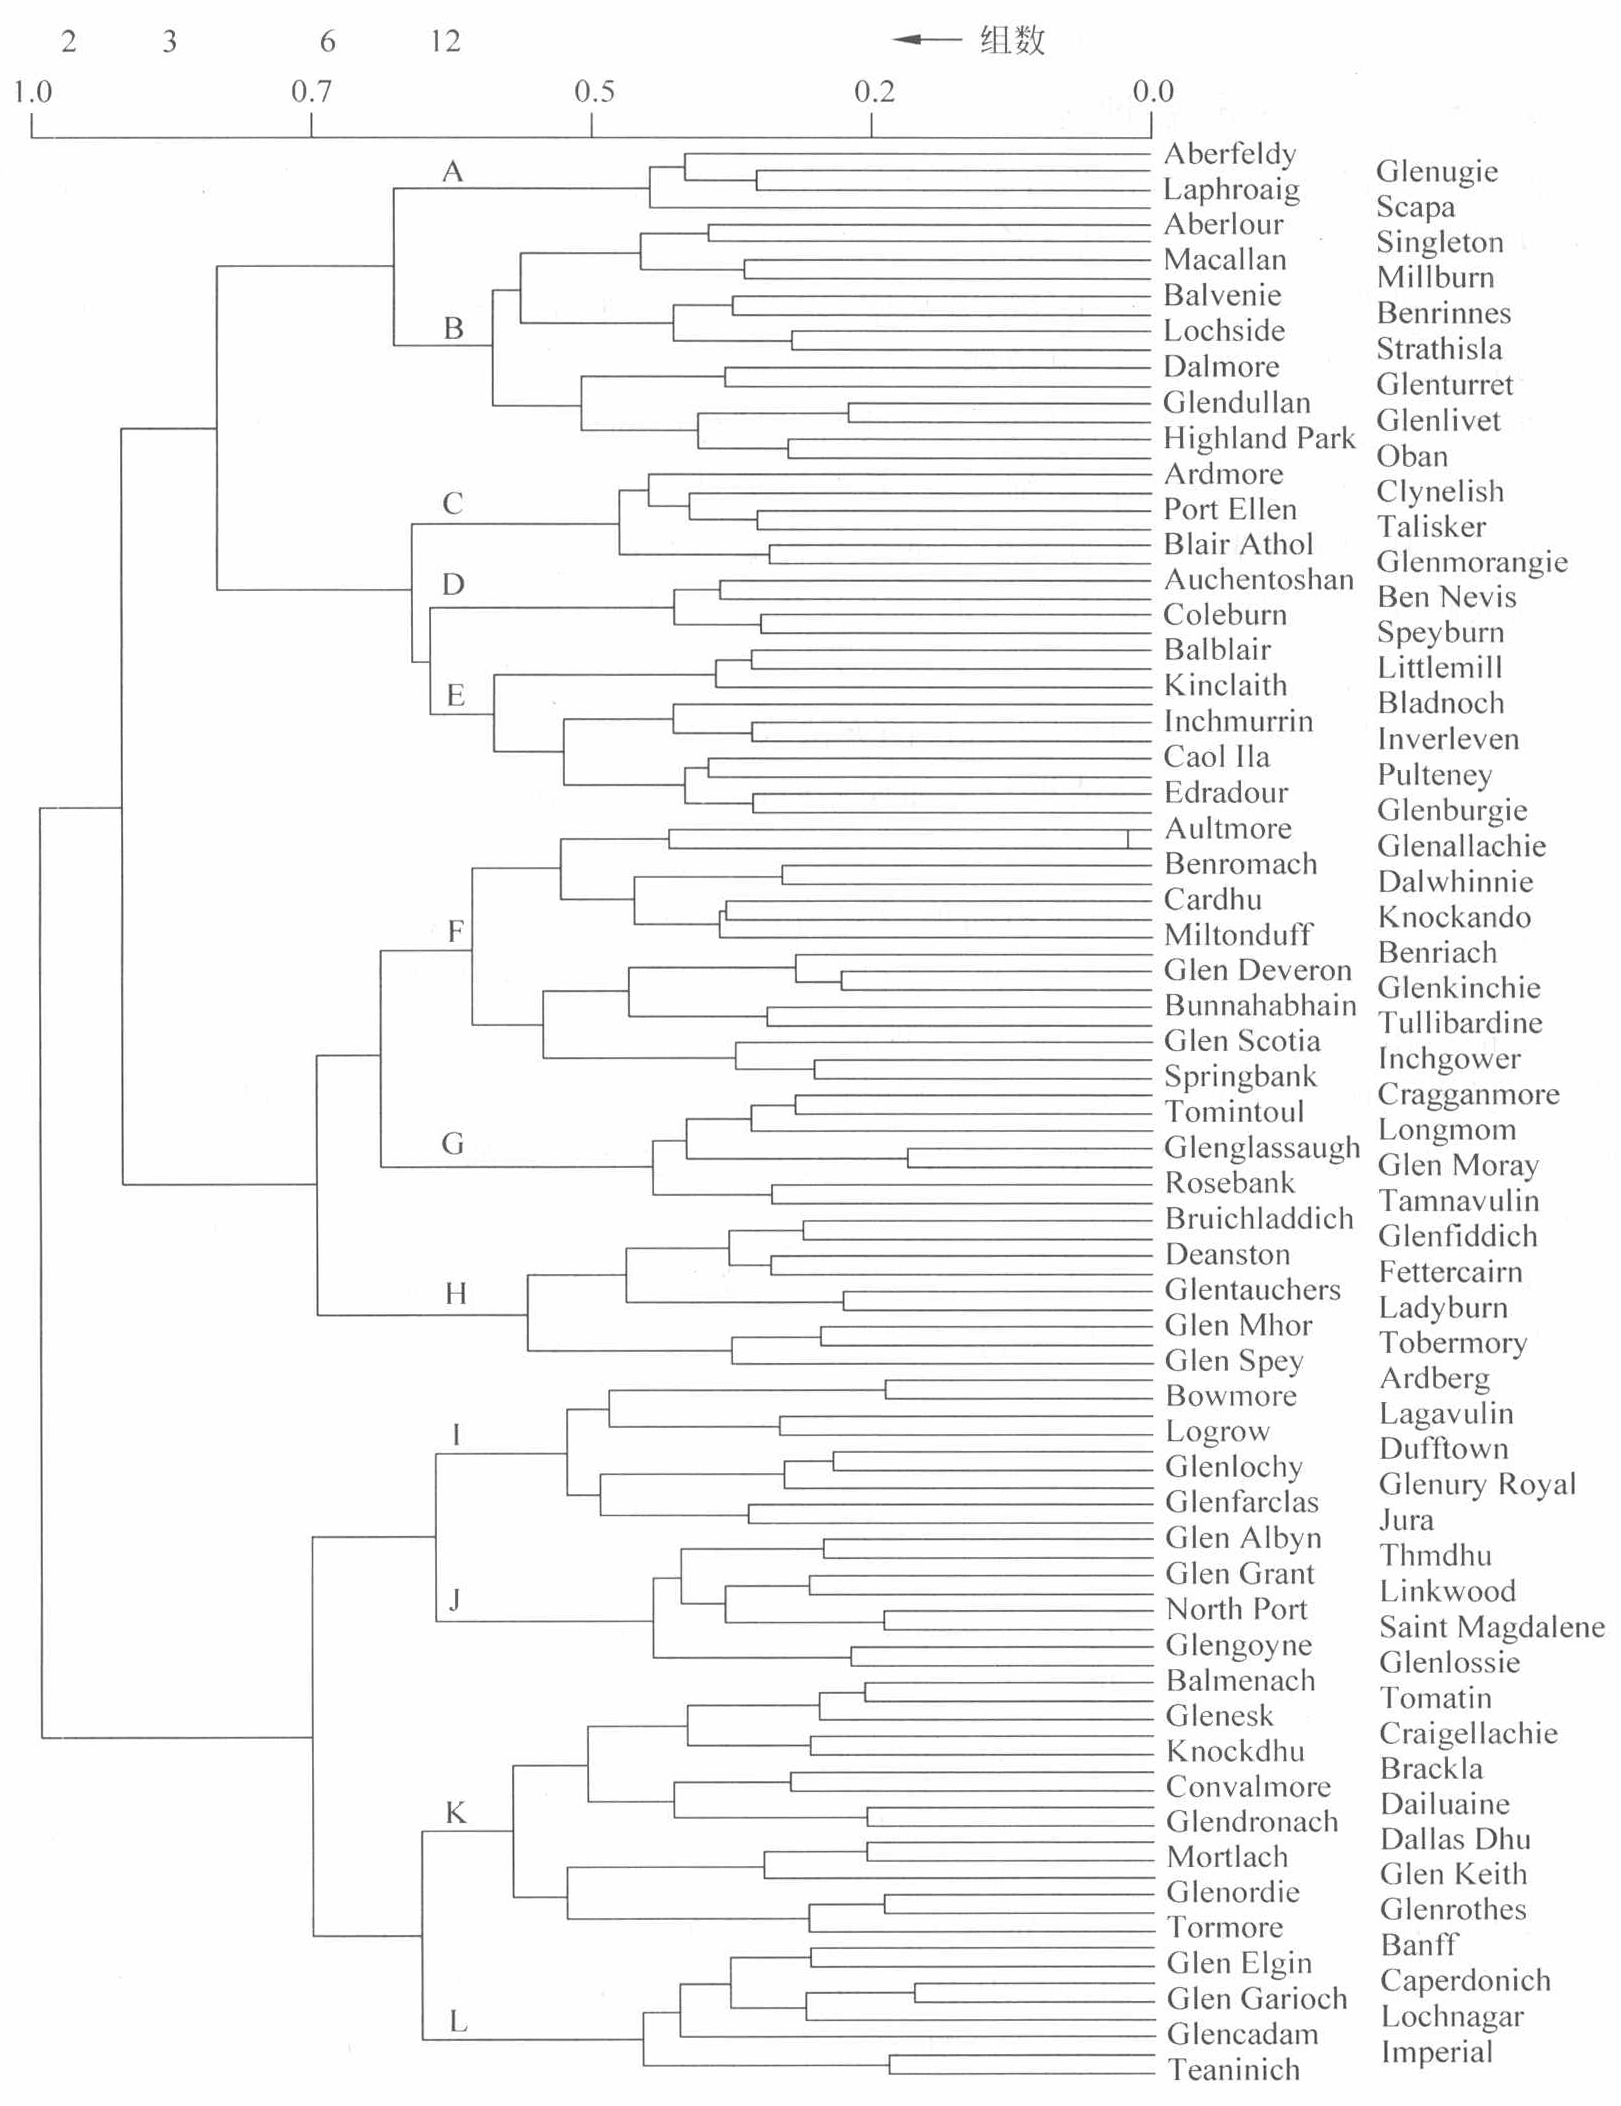
\includegraphics[width=137.3mm]{figs/fig_pg553_1.png}
\phantomsection\label{fig:12.11}\mvcap{图 12.11\quad 109 种纯麦芽苏格兰威士忌之间相似性的树图}
\end{mvfigure}

\vspace{0.4em}
\noindent\rule{\linewidth}{0.4pt}

{\zihao{6}
\noindent * 树图中标有字母 A 至 L 的 12 个组是经研究者识别后认为是相似的. 随后的分析表明, 这 12 个组受到某个很大的地理成分的支配.
也就是说, 位置互相靠近的那些酒厂倾向于生产具有类似特性的威士忌. 于是这些研究人员得出结论: “与地理特征的关系已被证实.
分析结果支持如下假设: 威士忌不仅受到厂家生产秘方和传统的影响, 而且还受到与地区有关的诸如\par}

%% ===== pg-554 =====

% ---- pg-554 （书页 542） ----

水、土壤、小气候、温度甚至空气质量等因素的影响.” \hfill$\blacksquare$

\mvsub{对分层方法的最后评注}

除了单连接、完全连接和平均连接之外, 还有许多聚集型分层聚类方法. 然而, 所有聚集型方法都遵循式(12-12) 中的基本算法.

同大多数聚类方法一样, 在分层方法中, 误差和变差来源并未得到正式考虑. 这就意味着聚类方法对离群值或“噪音点”很敏感.

在分层聚类中, 对于那些在早期阶段被“错误”分组的对象不提供重新分组的机会. 因此, 始终应对最终的聚类结构进行仔细检查, 看看结果是否合情合理.

对某个特定的问题, 较好的做法是试用几种聚类方法, 而对一种给定的方法, 可以试用几种不同的距离(相似性).
如果用几种不同方法得到的结果(大体上)彼此一致, 那么就有可能找到一个“自然”分组.

某个分层解的稳定性有时可用这样的方法来检查: 对数据单元加进一些小误差(干扰), 然后运用聚类算法, 并将新的结果与未加误差时的结果进行比较.
如果各组数据能很好区分, 则两种结果应大体吻合.

距离矩阵或相似性矩阵中的相同值(结)有可能使分层聚类问题产生多重解. 也就是说, 用不同方法处理打结的相似性(距离)会得出不同的树图, 特别是在较低的水平上.
并非任何方法都会出现这种问题, 只有特定类型的数据才会发生多重解. 出现多重解未必是坏事.
不过聚类方法的应用者应该知道这种现象的存在, 以便对分组(树图)给出恰当的解释, 并比较不同的分组(树图), 以评估它们的重合程度.
对这个问题的进一步讨论可在文献[27]中找到.

某些数据集和分层聚类方法会产生“逆序”(见文献[27]).
当某个对象在并入一个已有的聚类时其距离小于上一次合并的距离, 就会发生逆序. 在下图中, 用两种不同方法代表一个逆序.

\begin{mvfigure}
\begin{minipage}[t]{0.44\linewidth}\centering
\begin{tikzpicture}[x=0.62cm,y=0.055cm,line width=0.4pt]
% 坐标轴
\draw (-0.72,0) -- (-0.72,38);
\draw (-0.72,0)  -- (-0.45,0);   \node[anchor=east,font=\fontsize{5}{6}\selectfont,inner sep=1pt] at (-0.78,0)  {0};
\draw (-0.72,20) -- (-0.45,20);  \node[anchor=east,font=\fontsize{5}{6}\selectfont,inner sep=1pt] at (-0.78,20) {20};
\draw (-0.72,30) -- (-0.45,30);  \node[anchor=east,font=\fontsize{5}{6}\selectfont,inner sep=1pt] at (-0.78,30) {30};
\draw (-0.72,32) -- (-0.45,32);  \node[anchor=east,font=\fontsize{5}{6}\selectfont,inner sep=1pt] at (-0.78,32) {32};
% 树图
\draw (0,0) -- (0,20);
\draw (1,0) -- (1,20);
\draw (0,20) -- (1,20);
\draw (0.5,20) -- (0.5,32);
\draw (0.5,32) -- (2,32);
\draw (1.25,32) -- (1.25,30);
\draw (1.25,30) -- (3,30);
\draw (1.25,32) -- (1.25,38);
\draw (2,0) -- (2,32);
\draw (3,0) -- (3,30);
% 叶子
\foreach \i/\lb in {0/A,1/B,2/C,3/D} {
  \node[font=\fontsize{6}{7}\selectfont,inner sep=1pt,anchor=north,yshift=-2pt] at (\i,0) {\lb};
}
\node[font=\fontsize{6}{7}\selectfont,inner sep=4pt] at (1.5,-11) {(a)};
\end{tikzpicture}
\end{minipage}\hfill
\begin{minipage}[t]{0.44\linewidth}\centering
\begin{tikzpicture}[x=0.62cm,y=0.055cm,line width=0.4pt]
% 坐标轴
\draw (-0.72,0) -- (-0.72,38);
\draw (-0.72,0)  -- (-0.45,0);   \node[anchor=east,font=\fontsize{5}{6}\selectfont,inner sep=1pt] at (-0.78,0)  {0};
\draw (-0.72,20) -- (-0.45,20);  \node[anchor=east,font=\fontsize{5}{6}\selectfont,inner sep=1pt] at (-0.78,20) {20};
\draw (-0.72,30) -- (-0.45,30);  \node[anchor=east,font=\fontsize{5}{6}\selectfont,inner sep=1pt] at (-0.78,30) {30};
\draw (-0.72,32) -- (-0.45,32);  \node[anchor=east,font=\fontsize{5}{6}\selectfont,inner sep=1pt] at (-0.78,32) {32};
% 树图
\draw (0,0) -- (0,20);
\draw (1,0) -- (1,20);
\draw (0,20) -- (1,20);
\draw (0.5,20) -- (0.5,30);
\draw (0.5,30) -- (2,30);
\draw (1.25,30) -- (1.25,32);
\draw (1.25,32) -- (3,32);
\draw (2.125,32) -- (2.125,38);
\draw (2,0) -- (2,30);
\draw (3,0) -- (3,32);
% 叶子
\foreach \i/\lb in {0/A,1/B,2/C,3/D} {
  \node[font=\fontsize{6}{7}\selectfont,inner sep=1pt,anchor=north,yshift=-2pt] at (\i,0) {\lb};
}
\node[font=\fontsize{6}{7}\selectfont,inner sep=4pt] at (1.5,-11) {(b)};
\end{tikzpicture}
\end{minipage}
\end{mvfigure}

在此例中, A 和 B 在距离 20 处合并. 下一步, C 在距离 32 处被加进(AB)组.
由于聚类算法的性质, D 在距离 30 处被加进(ABC)组. 这个距离小于 C 被加进(AB)组时的距离.
在图 (a) 中, 逆序由一个带交叉的树图表示. 在图 (b) 中, 逆序由一个具有非单调尺度的树图表示.

在没有清晰的聚类结构的情况下, 就会出现逆序, 因此逆序一般与两种分层聚类算法(即中心方法和中位数方法)相联系.
本书中所讨论的分层方法不易产生逆序.

\section{非分层聚类方法}
\phantomsection\label{sec:12.4}

设计非分层聚类技术的目的是, 为了将项目(不是变量)分成由 $K$ 个聚类组成的集合.
聚类的个数 $K$ 可以事先指定, 也可以在聚类过程中确定. 由于在计算机运行过程中不必确定距

%% ===== pg-555 =====

% ---- pg-555 （书页 543） ----

离(相似性)矩阵, 也不必存储基本数据, 所以同分层方法相比, 非分层方法可用于大得多的数据集.

非分层方法的起点或者是(1)一个初始的分割, 或者是(2)构成未来聚类核心的一组初始种子点. 好的初始结构应该没有明显的偏倚.
一种起动方式是从项目中随机选出种子点, 或者将项目随机地分割成初始组的集合.

在这一节中, 我们将讨论一种比较流行的非分层方法——$K$ 均值法.

\mvsub{$K$ 均值法}

麦奎因(MacQueen, 见文献[25])将他所提出的一种算法命名为 $K$ 均值法. 这种算法的基本思想是将每一个项目分给具有最近中心(均值)的聚类.
最简单形式中的算法包括以下三个步骤:

\noindent 1.\quad 将所有项目分成 $K$ 个初始聚类.

\noindent 2.\quad 将项目表中的某个项目划入中心(均值)离它最近的聚类. (这里的距离通常是用标准化或非标准化数据算出的欧氏距离.) 对得到项目和失去项目的两个聚类重新计算它们的中心坐标.

\noindent 3.\quad 重复步骤 2, 直至所有的点都不能再分配时为止. \hfill (12-16)

\noindent 在上述过程中, 步骤 1 也可以不从分割出 $K$ 个初始聚类开始, 而从规定 $K$ 个初始中心(种子点)开始, 然后进入步骤 2.

最终的分类结果在某种程度上依赖于初始分组或初始种子点的选择. 经验显示, 聚类过程中的绝大多数重要变化均发生在第一次再分配中.

\noindent\textbf{例 12.11}\quad (用 $K$ 均值法聚类)

假定我们对 $A,B,C,D$ 四个项目分别测量两个变量 $x_1$ 和 $x_2$, 得到如下数据:

\begin{mvtable}
\footnotesize
\begin{tabular}{lcc}
\toprule
\multirow{2}{*}{项\quad 目} & \multicolumn{2}{c}{变\quad 量}\\
\cmidrule(lr){2-3}
 & $x_1$ & $x_2$\\
\midrule
$A$ & 5 & 3\\
$B$ & $-1$ & 1\\
$C$ & 1 & $-2$\\
$D$ & $-3$ & $-2$\\
\bottomrule
\end{tabular}
\end{mvtable}

我们的目标是将这些项目分成 $K=2$ 个聚类, 使每个聚类内部的项目之间的距离比与分别属于不同聚类的项目之间的距离小.
为了实施 $K=2$ 均值法, 我们将这些项目先随意分成两个聚类, 比如说 $(AB)$ 和 $(CD)$, 然后计算这两个聚类的中心(均值)的坐标 $(\bar{x}_1,\bar{x}_2)$.
这样, 在步骤 1 中我们有:

\begin{mvtable}
\footnotesize
\begin{tabular}{lcc}
\toprule
\multirow{2}{*}{聚\quad 类} & \multicolumn{2}{c}{中心的坐标}\\
\cmidrule(lr){2-3}
 & $\bar{x}_1$ & $\bar{x}_2$\\
\midrule
$(AB)$ & $\dfrac{5+(-1)}{2}=2$ & $\dfrac{3+1}{2}=2$\\[6pt]
$(CD)$ & $\dfrac{1+(-3)}{2}=-1$ & $\dfrac{-2+(-2)}{2}=-2$\\
\bottomrule
\end{tabular}
\end{mvtable}

%% ===== pg-556 =====

% ---- pg-556 （书页 544） ----

在第二步中, 我们计算每一项到组中心的欧氏距离, 并将其重新归入最近的组. 如果某一项从原来的结构中移动了, 则类中心(均值)必须更新.
中心的第 $i$ 个坐标, $i=1,\cdots,p$, 可用以下公式更新:
\[
\bar{x}_{i,\text{new}}=\frac{n\bar{x}_i+x_{ji}}{n+1}, \qquad \text{若第 } j \text{ 项加入到组 } i,
\]
\[
\bar{x}_{i,\text{new}}=\frac{n\bar{x}_i-x_{ji}}{n-1}, \qquad \text{若第 } j \text{ 项从组 } i \text{ 移除}
\]
其中 $n$ 是旧组中项目的数目, 其中心为 $\bar{\mathbf{x}}'_i=(\bar{x}_{i1},\cdots,\bar{x}_{ip})$.

考虑初始类 $(AB)$ 和 $(CD)$. 中心坐标分别为 $(2,2)$ 和 $(-1,-2)$. 假设项目 $A$ 被移到组 $(CD)$ 中, 则新的组为 $(B)$ 和 $(ACD)$, 更新后的中心为:
\[
\begin{aligned}
\text{组 }(B)\qquad \bar{x}_{1,\text{new}}&=\frac{2\times 2-5}{2-1}=-1 &\qquad
\bar{x}_{2,\text{new}}&=\frac{2\times 2-3}{2-1}=1, \qquad \text{即 } B \text{ 的坐标}\\
\text{组 }(ACD)\qquad \bar{x}_{1,\text{new}}&=\frac{2\times(-1)+5}{2+1}=1 &\qquad
\bar{x}_{2,\text{new}}&=\frac{2\times(-2)+3}{2+1}=-0.33
\end{aligned}
\]

回到步骤 1 中的初始分组, 我们计算距离平方
\[
\begin{aligned}
d^{2}(A,(AB))&=(5-2)^{2}+(3-2)^{2}=10 &&\text{若 } A \text{ 不移动}\\
d^{2}(A,(CD))&=(5+1)^{2}+(3+2)^{2}=61
\end{aligned}
\]
\[
\begin{aligned}
d^{2}(A,(B))&=(5+1)^{2}+(3-1)^{2}=40 &&\text{若 } A \text{ 移动到组 }(CD)\\
d^{2}(A,(ACD))&=(5-1)^{2}+(3+0.33)^{2}=27.09
\end{aligned}
\]
由于 $A$ 到组 $(AB)$ 中心的距离小于到组 $(ACD)$ 中心的距离, 因此 $A$ 不更换组.

我们继续考虑 $B$ 是否更换组的问题. 我们有
\[
\begin{aligned}
d^{2}(B,(AB))&=(-1-2)^{2}+(1-2)^{2}=10 &&\text{若 } B \text{ 不移动}\\
d^{2}(B,(CD))&=(-1+1)^{2}+(1+2)^{2}=9
\end{aligned}
\]
\[
\begin{aligned}
d^{2}(B,(A))&=(-1-5)^{2}+(1-3)^{2}=40 &&\text{若 } B \text{ 移动到组 }(CD)\\
d^{2}(B,(BCD))&=(-1+1)^{2}+(1+1)^{2}=4
\end{aligned}
\]
由于 $B$ 到组 $(BCD)$ 中心的距离小于到组 $(AB)$ 中心的距离, 因此 $B$ 更换组到组 $(CD)$. 于是我们得到类 $(A)$ 和 $(BCD)$, 中心分别为 $(5,3)$ 和 $(-1,-1)$.

我们考虑 $C$ 的更换问题. (译者注: 在新的分类 $(A)$ 和 $(BCD)$ 的前提下.)
\[
\begin{aligned}
d^{2}(C,(A))&=(1-5)^{2}+(-2-3)^{2}=41 &&\text{若 } C \text{ 不移动}\\
d^{2}(C,(BCD))&=(1+1)^{2}+(-2+1)^{2}=5
\end{aligned}
\]
\[
\begin{aligned}
d^{2}(C,(AC))&=(1-3)^{2}+(-2-0.5)^{2}=10.25 &&\text{若 } C \text{ 移动到组 }(A)\\
d^{2}(C,(BD))&=(1+1)^{2}+(-2+0.5)^{2}=11.25
\end{aligned}
\]
由于 $C$ 到组 $(BCD)$ 中心的距离小于到组 $(AC)$ 中心的距离, 因此 $C$ 不移动.
如此继续, 我们发现: 没有更换再发生, 最终的 $K=2$ 类为 $(A)$ 和 $(BCD)$.

对最终的类, 我们有

\begin{mvtable}
\footnotesize
\begin{tabular}{lcccc}
\toprule
& \multicolumn{4}{c}{到组中心的距离平方}\\
\cmidrule(lr){2-5}
\multirow{2}{*}{类} & \multicolumn{4}{c}{项\quad 目}\\
\cmidrule(lr){2-5}
& $A$ & $B$ & $C$ & $D$\\
\midrule
$A$ & 0 & 40 & 41 & 89\\
$(BCD)$ & 52 & 4 & 5 & 5\\
\bottomrule
\end{tabular}
\end{mvtable}

%% ===== pg-557 =====

% ---- pg-557 （书页 545） ----

组内平方和(到中心的距离平方和)为

\hspace*{6em}类 $A$:\hfill 0

\hspace*{6em}类 $(BCD)$:\hfill $4+5+5=14$

等价地, 我们可以用准则
\[
\min E=\sum d^{2}_{i,\text{类}(i)}
\]
确定 $K=2$ 个类, 其中最小化是对所有 $K=2$ 个类的聚类, $d^{2}_{i,\text{类}(i)}$ 是从项目 $i$ 到其所在类的中心的距离平方.

在此例中, 总共有 7 个可能的 $K=2$ 个类的聚类:

\hspace*{4em}$A,(BCD)$

\hspace*{4em}$B,(ACD)$

\hspace*{4em}$C,(ABD)$

\hspace*{4em}$D,(ABC)$

\hspace*{4em}$(AB),(CD)$

\hspace*{4em}$(AC),(BD)$

\hspace*{4em}$(AD),(BC)$

\noindent 对于聚类 $\{A,(BCD)\}$:

\hspace*{6em}$A$:\hfill $d^{2}_{A,\text{类}(A)}=0$

\hspace*{6em}$(BCD)$:\hfill $d^{2}_{B,\text{类}(B)}+d^{2}_{C,\text{类}(C)}+d^{2}_{D,\text{类}(D)}=4+5+5=14$

因此 $\sum d^{2}_{i,\text{类}(i)}=0+14=14$.

\noindent 对于其他聚类, 不难验证

\begin{mvtable}
\begin{tabular}{lcccc}
& $B,(ACD)$ & & $\sum d^{2}_{i,\text{类}(i)}$ & $=48.7$\\[4pt]
& $C,(ABD)$ & & $\sum d^{2}_{i,\text{类}(i)}$ & $=27.7$\\[4pt]
& $D,(ABC)$ & & $\sum d^{2}_{i,\text{类}(i)}$ & $=31.3$\\[4pt]
& $(AB),(CD)$ & & $\sum d^{2}_{i,\text{类}(i)}$ & $=28$\\[4pt]
& $(AC),(BD)$ & & $\sum d^{2}_{i,\text{类}(i)}$ & $=27$\\[4pt]
& $(AD),(BC)$ & & $\sum d^{2}_{i,\text{类}(i)}$ & $=51.3$
\end{tabular}
\end{mvtable}

由于聚类 $\{A,(BCD)\}$ 有最小 $\sum d^{2}_{i,\text{类}(i)}$, 这是最终得到的划分. \hfill$\blacksquare$

为检查聚类结果的稳定性, 应该以新的初始分割重新启动算法. 一旦聚类被确定, 就可通过对项目表中诸项目的重新排列来对聚类作直观解释:
使处于第一个聚类中的项目排在最前面, 处于第二个聚类中的项目排在下一个位置, 等等.
一份列有各聚类中心坐标和每个聚类内部方差的表同样有助于刻画组与组之间的差别.

\noindent\textbf{例 12.12}\quad (对公用事业公司进行聚类的 $K$ 均值法)

我们回到对公用事业公司进行聚类的问题, 其由数据由\hyperref[tab:12.4]{表 12.4} 中给出. 这次采用 $K$ 均值法, 并对 $K$ 取若干不同的值.
我们把 $K=4$ 和 $K=5$ 时分类结果汇总如下表. 一般来说, 特定 $K$ 值的选择并不是明确无误的, 这依赖于对分类对象的背景知识和基于数据的评估.
(基于数据的评估也许包括选择 $K$ 值, 以使组间变差相对组内变差达到极大. 有关的量度可以是 $|\mathbf{W}|/|\mathbf{B}+\mathbf{W}|$ [见\hyperref[eq:6-38]{式(6-38)}] 和 $\mathrm{tr}(\mathbf{W}^{-1}\mathbf{B})$.

%% ===== pg-558 =====

% ---- pg-558 （书页 546） ----

\noindent $K=4$

\begin{mvtable}
\footnotesize
\setlength{\tabcolsep}{4pt}%
\begin{tabular}{ccp{9.2cm}}
\toprule
聚类 & 聚类中的公司数目 & \multicolumn{1}{c}{公\quad\quad 司}\\
\midrule
1 & 5 & 爱达荷电力公司(8), 内华达电力公司(11), 普盖特桑德电力与电灯公司(16), 弗吉尼亚电气与电力公司(22), 肯塔基公用事业公司(9)\\
2 & 6 & 中央路易斯安那电气公司(3), 俄克拉何马天然气与电力公司(14), 南方公司(18), 得克萨斯公用事业公司(19), 亚利桑那公共服务公司(1), 佛罗里达电力与电灯公司(6)\\
3 & 5 & 新英格兰电气公司(12), 太平洋天然气与电力公司(15), 圣地亚哥天然气与电力公司(17), 联合照明公司(21), 夏威夷电气公司(7)\\
4 & 6 & 联合爱迪生公司(纽约)(5), 波士顿爱迪生公司(2), 麦迪逊天然气与电力公司(10), 北方电力公司(13), 威斯康星电力公司(20), 联邦爱迪生公司(4)\\
\bottomrule
\end{tabular}
\end{mvtable}

\begin{mvtable}
\mvtabcap{聚类中心之间的距离}
\[
\begin{array}{ccccc}
 & 1 & 2 & 3 & 4\\
1 & 0 & & & \\
2 & 3.08 & 0 & & \\
3 & 3.29 & 3.56 & 0 & \\
4 & 3.05 & 2.84 & 3.18 & 0
\end{array}
\]
\end{mvtable}

\noindent $K=5$

\begin{mvtable}
\footnotesize
\setlength{\tabcolsep}{4pt}%
\begin{tabular}{ccp{9.2cm}}
\toprule
聚类 & 聚类中的公司数目 & \multicolumn{1}{c}{公\quad\quad 司}\\
\midrule
1 & 5 & 内华达电力公司(11), 普盖特桑德电力与电灯公司(16), 爱达荷电力公司(8), 弗吉尼亚电气与电力公司(22), 肯塔基公用事业公司(9)\\
2 & 6 & 中央路易斯安那电气公司(3), 得克萨斯公用事业公司(19), 俄克拉何马天然气与电力公司(14), 南方公司(18), 亚利桑那公共服务公司(1), 佛罗里达电力与电灯公司(6)\\
3 & 5 & 新英格兰电气公司(12), 太平洋天然气与电力公司(15), 圣地亚哥天然气与电力公司(17), 联合照明公司(21), 夏威夷电气公司(7)\\
4 & 2 & 联合爱迪生公司(纽约)(5), 波士顿爱迪生公司(2)\\
5 & 4 & 联邦爱迪生公司(4), 麦迪逊天然气与电力公司(10), 北方电力公司(13), 威斯康星电力公司(20)\\
\bottomrule
\end{tabular}
\end{mvtable}

\begin{mvtable}
\mvtabcap{聚类中心之间的距离}
\[
\begin{array}{cccccc}
 & 1 & 2 & 3 & 4 & 5\\
1 & 0 & & & & \\
2 & 3.08 & 0 & & & \\
3 & 3.29 & 3.56 & 0 & & \\
4 & 3.63 & 3.46 & 2.63 & 0 & \\
5 & 3.18 & 2.99 & 3.81 & 2.89 & 0
\end{array}
\]
\end{mvtable}

$K=5$ 时的各种聚类轮廓图示于\hyperref[fig:12.12]{图 12.12}. 图中八个变量按组间变差与组内变差之比从大到小的顺序排列(对单变量的 $F$ 比, 见 6.4 节). 我们有

%% ===== pg-559 =====

% ---- pg-559 （书页 547） ----

\begin{mvfigure}
\resizebox{\linewidth}{!}{\rotatebox{-90}{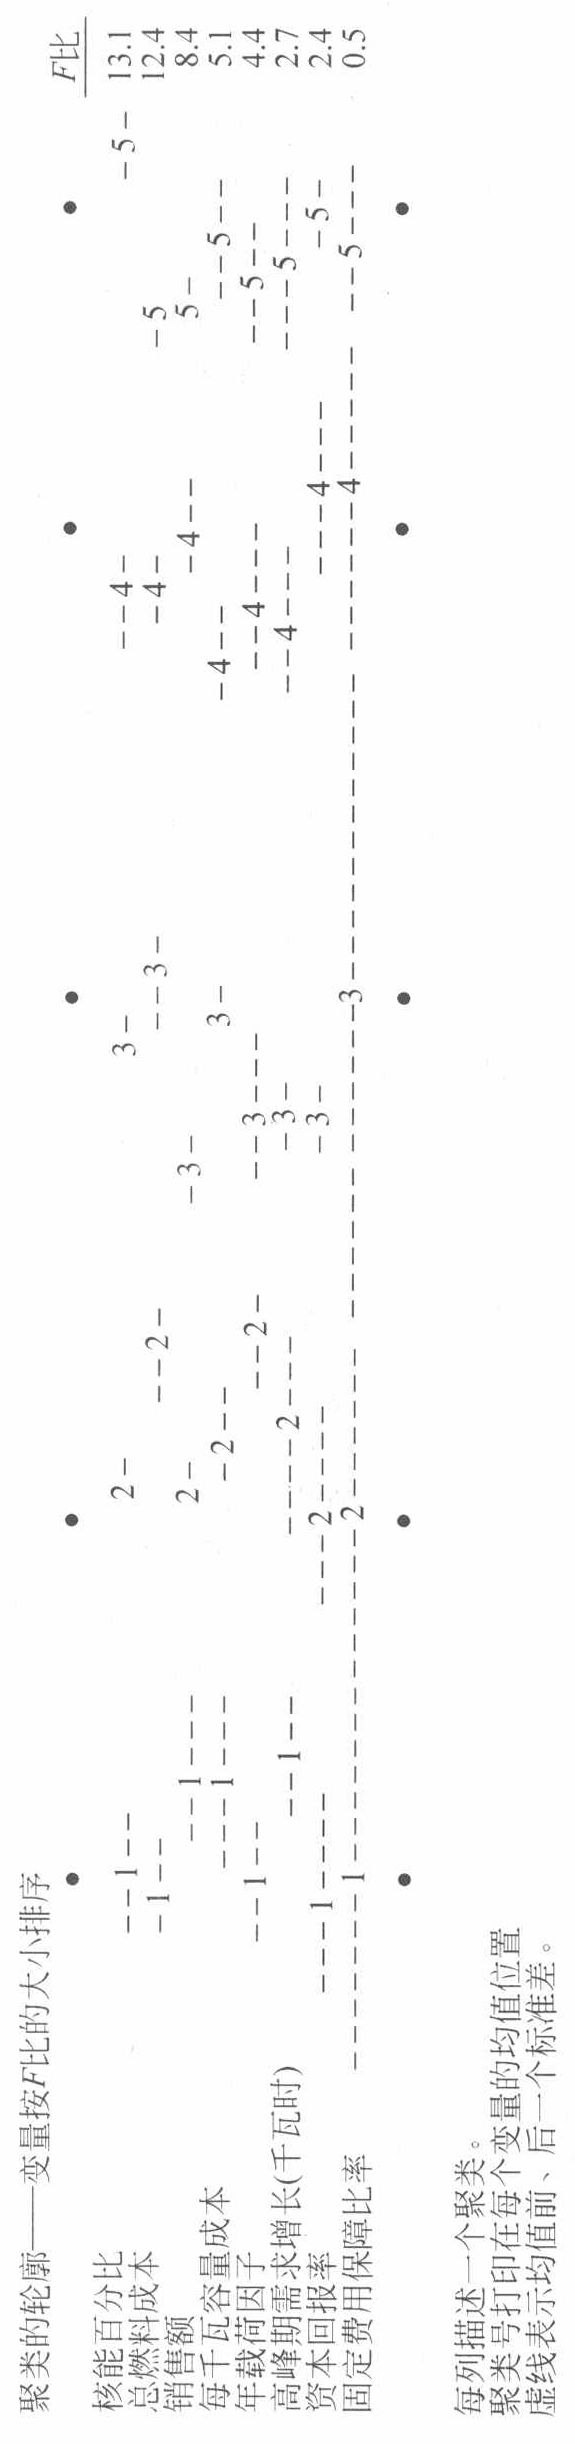
\includegraphics[width=48.6mm]{figs/fig_pg559_1.png}}}
\phantomsection\label{fig:12.12}\mvcap{图 12.12\quad 公用事业公司数据在 $K=5$ 时的聚类轮廓图}
\end{mvfigure}

%% ===== pg-560 =====

% ---- pg-560 （书页 548） ----

\[
F_{\text{nuc}}=\frac{\text{聚类间核能百分比的均方}}{\text{聚类内核能百分比的均方}}=\frac{3.335}{0.255}=13.1
\]
可见不同聚类的公司之间的核能百分比弥散度很大, 而同一聚类内部的公司其核能百分比的变差很小. 燃料成本和年销售额在区分聚类方面看来也有某种重要性.

回顾五个聚类中的公司可以看到, $K$ 均值法给出的结果一般与平均连接分层法的结果一致(见例 12.9). 具有相同或相容地理位置的公司聚集在一起.
还有, 处于同一聚类中的公司其核能百分比大致相同. \hfill$\blacksquare$

正如我们在全书一直强调的那样, 在聚类过程中评价单个变量的重要性时一定要小心, 这种评价必须从多元的角度判断.
所有变量(多元观测值)决定各个聚类均值和各个项目的归属. 此外, 量度个别变量重要性的描述性统计量的值是聚类个数及最终聚类结构的函数.
另一方面, 在得出结果之后, 有些描述性量度可能有助于评估聚类方法是否“成功”.

\mvsub{对非分层方法的最后评注}

对非分层方法在事先不固定聚类数目 $K$ 的问题上有很多争议. 争议包括以下几点:

\noindent 1.\quad 若两个或更多个种子点碰巧处于同一聚类之中, 所得到的最终聚类会难以区分.

\noindent 2.\quad 当存在某个离群值时, 至少会产生一个所含项目非常分散(不集中)的聚类.

\noindent 3.\quad 即使知道总体由 $K$ 个组组成, 抽样过程也有可能产生这样的结果: 来自最稀疏的那一组的数据未出现在样本之中. 这种情况之下, 强行将数据分成 $K$ 组会造成某些毫无意义的聚类.

\noindent 当某一次算法运行中需要用户指定 $K$ 值时, 使这种算法对若干个不同的初值重复运行多次, 始终是一个不错的想法.

其他关于非分层聚类方法的讨论可从文献[3], [8]和[16]中找到.

\section{基于统计模型的聚类}
\phantomsection\label{sec:12.5}

本章前面讨论了若干常用聚类方法, 包括单连接、完全连接、平均连接、王尔德方法, 以及 $K$ 均值聚类等.
这些方法都是直观上合理的聚类程序, 但是都没有模型来解释观测数据是如何产生的.
通过在聚类方法中引进统计模型, 最大的好处就是可以解释 $(p\times 1)$ 维度量 $\mathbf{x}_j$ 是如何从 $N$ 个对象中产生的.
最常用的模型是假定类 $k$ 中的对象所占的期望比例为 $p_k$, 而相应的度量变量的参数有概率密度函数 $f_k(\mathbf{x})$.
如此, 若有 $K$ 个类, 从单个对象得到的观测向量可认为是从一个混合分布中得到, 其概率密度函数为
\[
f_{\text{Mix}}(\mathbf{x})=\sum_{k=1}^{K}p_k f_k(\mathbf{x})
\]
其中 $p_k\ge 0$ 且 $\sum\limits_{k=1}^{K}p_k=1$. 分布 $f_{\text{Mix}}(\mathbf{x})$ 称为是 $K$ 个分布 $f_k(\mathbf{x})$ 的混合物, $k=1,\cdots,K$.
从这个分布中生成的 $N$ 个观测是从分量分布中得到的观测的混合物.

最常用的混合模型是多元正态分布的混合物, 其中 $f_k(\mathbf{x})$ 是 $N_p(\boldsymbol{\mu}_k,\boldsymbol{\Sigma}_k)$ 的密度函数.
对于观测 $\mathbf{x}$, 正态混合模型的密度函数为

\phantomsection\label{eq:12-17}
\begin{equation}
\begin{aligned}
&f_{\text{Mix}}(\mathbf{x}\mid \boldsymbol{\mu}_1,\boldsymbol{\Sigma}_1,\cdots,\boldsymbol{\mu}_K,\boldsymbol{\Sigma}_K)\\
&\quad=\sum_{k=1}^{K}p_k\frac{1}{(2\pi)^{p/2}|\boldsymbol{\Sigma}_k|^{1/2}}\exp\left(-\frac{1}{2}(\mathbf{x}-\boldsymbol{\mu}_k)'\boldsymbol{\Sigma}_k^{-1}(\mathbf{x}-\boldsymbol{\mu}_k)\right)
\end{aligned} \tag{12-17}
\end{equation}

由此模型产生的类有椭球形状, 在中心附近的集中度最高.

%% ===== pg-561 =====

% ---- pg-561 （书页 549） ----

对 $N$ 个观测和给定的 $K$ 个类, 似然函数为
\phantomsection\label{eq:12-18}
\begin{equation}
\begin{aligned}
&L(p_1,\cdots,p_K,\boldsymbol{\mu}_1,\boldsymbol{\Sigma}_1,\cdots,\boldsymbol{\mu}_K,\boldsymbol{\Sigma}_K) = \prod_{j=1}^{N} f_{\mathrm{Mix}}(\mathbf{x}_j\mid \boldsymbol{\mu}_1,\boldsymbol{\Sigma}_1,\cdots,\boldsymbol{\mu}_K,\boldsymbol{\Sigma}_K)\\
&\qquad = \prod_{j=1}^{N}\left\{ \sum_{k=1}^{K} p_k \frac{1}{(2\pi)^{p/2}|\boldsymbol{\Sigma}_k|^{1/2}}\exp\left( -\frac{1}{2}(\mathbf{x}_j-\boldsymbol{\mu}_k)'\boldsymbol{\Sigma}_k^{-1}(\mathbf{x}_j-\boldsymbol{\mu}_k) \right) \right\}
\end{aligned}
\tag{12-18}
\end{equation}
其中比例 $p_1,\cdots,p_K$, 均值向量 $\boldsymbol{\mu}_1,\cdots,\boldsymbol{\mu}_K$ 和协方差矩阵 $\boldsymbol{\Sigma}_1,\cdots,\boldsymbol{\Sigma}_K$ 是未知的. 不同对象的度量看成是从混合分布中抽出的独立同分布的观测.

当被聚类的对象的数量不太大时, 模型中的未知参数显得太多. 然而, 如果某种启发性有好的效果, 还可以得到某种程度的结论. 特别地, 如果所有协方差矩阵 $\boldsymbol{\Sigma}_k$ 都有 $\eta\mathbf{I}$ 的形式, 其中 $\eta$ 为未知因子, 则基于似然函数的程序大致相当于 $K$ 均值聚类和王尔德方法. 到目前为止, 还没有基于统计模型的聚类方法进展到相当于单连接、完全连接或平均连接的方法.

更重要的是, 对于不同 $K$ 的一系列混合模型(12-17), 选择类的数量和选择适当的聚类方法的问题转化为选择适当的统计模型的问题. 这是一个主要的优点.

选择模型的一个好办法是首先对给定的 $K$ 得到参数的极大似然估计 $\hat{p}_1,\cdots,\hat{p}_K,\hat{\boldsymbol{\mu}}_1,\cdots,\hat{\boldsymbol{\mu}}_K$ 和 $\hat{\boldsymbol{\Sigma}}_1,\cdots,\hat{\boldsymbol{\Sigma}}_K$. 这些估计只能用特别编制的软件求得数值解. 似然函数的极大值
\[
L_{\max} = L(\hat{p}_1,\cdots,\hat{p}_K,\hat{\boldsymbol{\mu}}_1,\hat{\boldsymbol{\Sigma}}_1,\cdots,\hat{\boldsymbol{\mu}}_K,\hat{\boldsymbol{\Sigma}}_K)
\]
提供模型选择的基础. 我们如何对类的数目 $K$ 确定一个合理的值? 为比较具有不同类数目的模型, 需要从二倍的对数极大似然值中减去一个惩罚项:
\[
2\ln L_{\max} - \text{惩罚项}
\]
其中惩罚项依赖于参数个数和观测个数 $N$. 由于概率 $p_k$ 之和为 1, 只有 $K-1$ 概率需要估计. 均值有 $K\times p$ 个, 方差-协方差有 $K\times p(p+1)/2$ 个. 对于赤池信息准则(AIC), 惩罚项为 $2N\times$(参数个数), 因此
\phantomsection\label{eq:12-19}
\begin{equation}
\text{AIC} = 2\ln L_{\max} - 2N\left( K\frac{1}{2}(p+1)(p+2)-1 \right) \tag{12-19}
\end{equation}
对于贝叶斯准则(BIC), 惩罚项中用观测个数的对数
\phantomsection\label{eq:12-20}
\begin{equation}
\text{BIC} = 2\ln L_{\max} - 2\ln(N)\left( K\frac{1}{2}(p+1)(p+2)-1 \right) \tag{12-20}
\end{equation}
但是, 混合模型中参数过多的问题仍然时有发生. 因此对 $\boldsymbol{\Sigma}_k$ 需要假定简单的结构. 下表具体给出一些从简单到较为复杂的协方差结构.

\begin{mvtable}
\begin{tabular}{lll}
\toprule
假定的 $\boldsymbol{\Sigma}_k$ 的形式 & 参数总数 & BIC\\
\midrule
$\boldsymbol{\Sigma}_k=\eta\mathbf{I}$ & $K(p+1)$ & $2\ln L_{\max}-2\ln(N)K(p+1)$\\
$\boldsymbol{\Sigma}_k=\eta_k\mathbf{I}$ & $K(p+2)-1$ & $2\ln L_{\max}-2\ln(N)(K(p+2)-1)$\\
$\boldsymbol{\Sigma}_k=\eta_k\mathit{Diag}\,(\lambda_1,\cdots,\lambda_p)$ & $K(p+2)+p-1$ & $2\ln L_{\max}-2\ln(N)(K(p+2)+p-1)$\\
\bottomrule
\end{tabular}
\end{mvtable}

更多的协方差矩阵结构在文献[6]和[9]中讨论.

即使对于固定的类数目, 混合模型的估计仍然是复杂的. 现有一个软件包 MCLUST 可从 R 软件库中得到. 此软件将分层聚类、EM 算法和 BIC 准则结合在一起, 发展出一个适合的模型用于聚类. 在 EM 算法的“E 步”, 创建一个 $(N\times K)$矩阵, 其第 $j$ 行包含观测 $\mathbf{x}_j$ 属于类 $1,\cdots,K$ 的(基于当前参数估计的)条件概率

%% ===== pg-562 =====

% ---- pg-562 （书页 550） ----

\[
p(k\mid \mathbf{x}_j) = \hat{p}_j f(\mathbf{x}_j\mid k)\Big/\sum_{i=1}^{K}\hat{p}_i f(\mathbf{x}_i\mid k)
\]

当程序收敛时, 第 $j$ 个观测(对象)被聚到具有最大条件概率的类 $k$(见文献[6]和[9]).

\noindent\textbf{例 12.13}\quad (鸢尾数据基于模型的聚类)

考虑\hyperref[tab:11.5]{表 11.5} 中的鸢尾数据. 用 MCLUST 中的 me 函数计算, 我们对 $p=4$ 维的正态混合模型进行拟合. 首先限制协方差矩阵为 $\boldsymbol{\Sigma}_k=\eta_k\mathbf{I}$, $k=1,2,3$.

用 BIC 准则, 软件计算结果选择了 $K=3$ 个类, 类中心的估计分别为
\[
\boldsymbol{\mu}_1=\begin{bmatrix}5.01\\3.43\\1.46\\0.25\end{bmatrix}, \qquad
\boldsymbol{\mu}_2=\begin{bmatrix}5.90\\2.75\\4.40\\1.43\end{bmatrix}, \qquad
\boldsymbol{\mu}_3=\begin{bmatrix}6.85\\3.07\\5.73\\2.07\end{bmatrix}
\]

方差尺度因子的估计分别为 $\hat{\eta}_1=0.076$, $\hat{\eta}_2=0.163$ 和 $\hat{\eta}_3=0.163$. 估计的混合比例分别为 $\hat{p}_1=0.333\,3$, $\hat{p}_2=0.413\,3$ 和 $\hat{p}_3=0.253\,4$. 相应的 BIC$=-853.8$. \hyperref[fig:12.13]{图 12.13} 给出了逐对变量聚类散点图的阵列.

\begin{mvfigure}
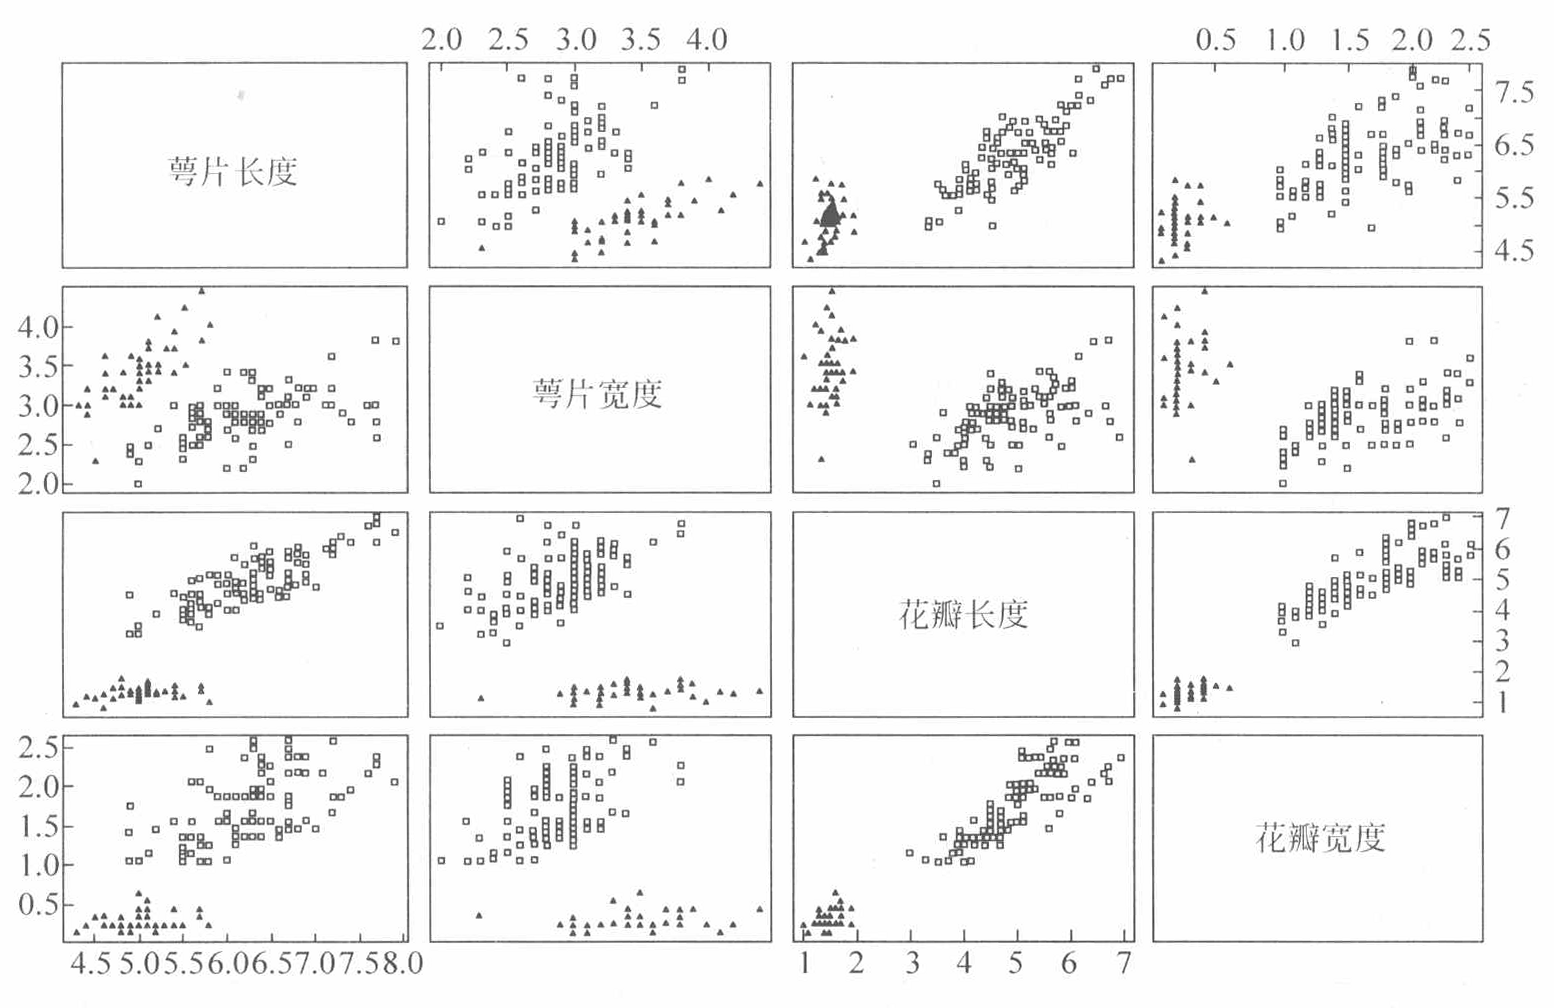
\includegraphics[width=131.6mm]{figs/fig_pg562_1.png}
\phantomsection\label{fig:12.13}\mvcap{图 12.13\quad 鸢尾数据分成 $K=3$ 类的多重散点图}
\end{mvfigure}

一旦得到了一个混合模型, 需要将新对象 $\mathbf{x}_j$ 归入某个类, $\mathbf{x}_j$ 在其中有最大的条件概率(见文献[9]).

如果假定协方差结构 $\boldsymbol{\Sigma}_k=\eta_k\mathbf{I}$, 并且允许最多达 $K=7$ 个类, 则 BIC 会增大到 BIC$=-705.1$.

最后, 在 BIC 准则下, 允许最多达 $K=9$ 个类, 并且使用几种不同的协方差结构, 得到的最佳选择是一个两类的混合模型, 其协方差是无约束的. 估计的混合概率为 $\hat{p}_1=0.333\,3$ 和 $\hat{p}_2=0.666\,7$. 估计的类中心为

%% ===== pg-563 =====

% ---- pg-563 （书页 551） ----

\[
\boldsymbol{\mu}_1=\begin{bmatrix}5.01\\3.43\\1.46\\0.25\end{bmatrix}, \qquad
\boldsymbol{\mu}_2=\begin{bmatrix}6.26\\2.87\\4.91\\1.68\end{bmatrix}
\]

两个估计的协方差矩阵为
\[
\hat{\boldsymbol{\Sigma}}_1=\begin{bmatrix}
0.121\,8 & 0.097\,2 & 0.016\,0 & 0.010\,1\\
0.097\,2 & 0.140\,8 & 0.011\,5 & 0.009\,1\\
0.016\,0 & 0.011\,5 & 0.029\,6 & 0.005\,9\\
0.010\,1 & 0.009\,1 & 0.005\,9 & 0.010\,9
\end{bmatrix}, \qquad
\hat{\boldsymbol{\Sigma}}_2=\begin{bmatrix}
0.453\,0 & 0.120\,9 & 0.448\,9 & 0.165\,5\\
0.120\,9 & 0.109\,6 & 0.141\,4 & 0.079\,2\\
0.448\,9 & 0.141\,4 & 0.674\,8 & 0.285\,8\\
0.165\,5 & 0.079\,2 & 0.285\,8 & 0.178\,6
\end{bmatrix}
\]

本质上, 两种鸢尾被归到一类里. 这一点可以从\hyperref[fig:12.14]{图 12.14} 中看出. \hyperref[fig:12.14]{图 12.14} 显示的是投影到萼片度量的散点图. \hfill$\blacksquare$

\begin{mvfigure}
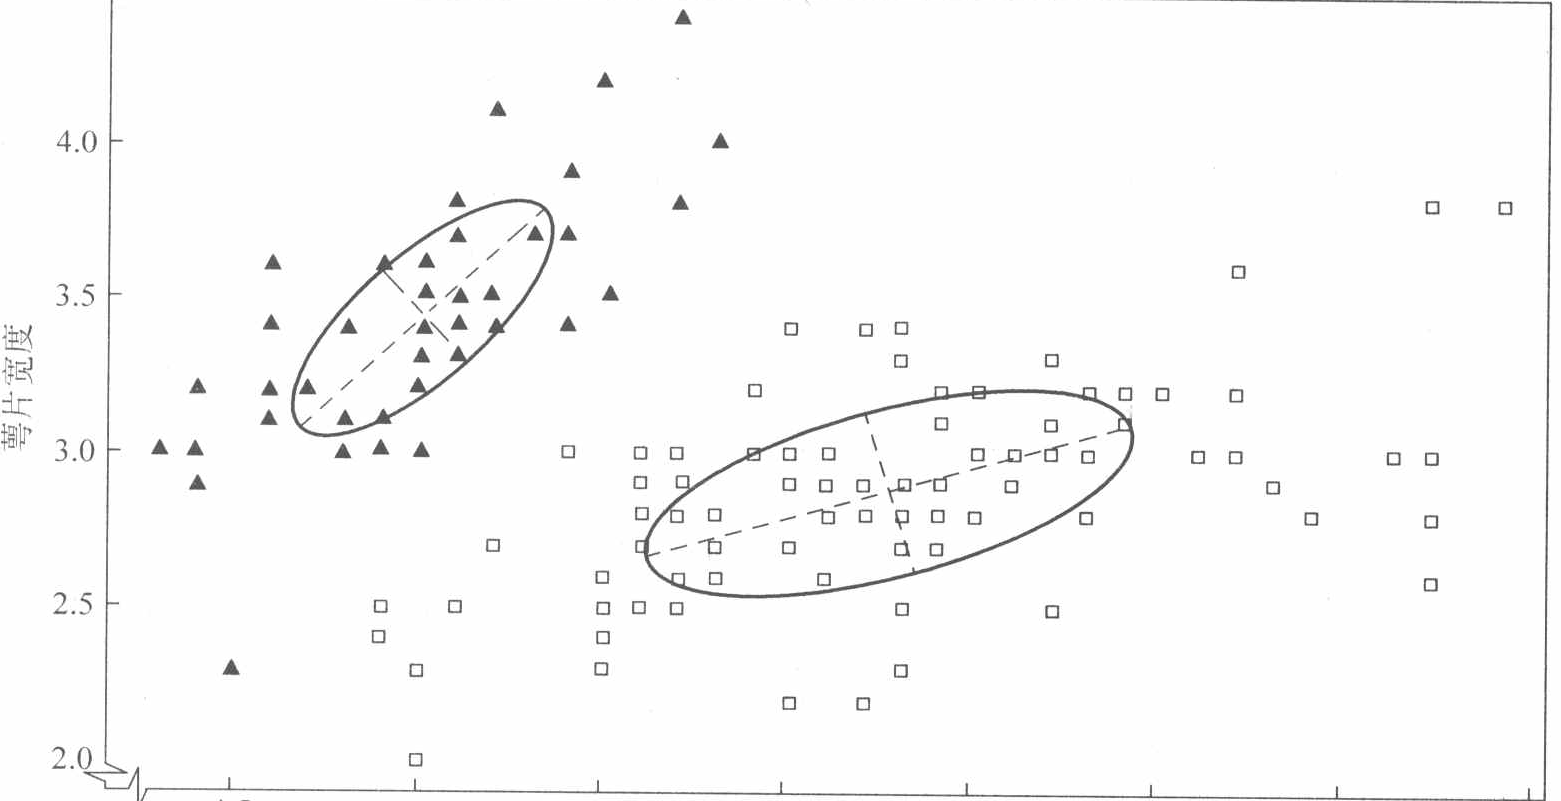
\includegraphics[width=132.1mm]{figs/fig_pg563_1.png}
\phantomsection\label{fig:12.14}\mvcap{图 12.14\quad 最佳模型对于萼片度量的散点图}
\end{mvfigure}

\vspace{0.5em}
\section{多维标度变换}
\phantomsection\label{sec:12.6}

本节讨论在低维空间展示(经过变换的)多元数据的方法. 我们在前面曾讨论过类似的问题, 例如对前两个主成分得分作图, 或者对前两个线性判别量的得分作图. 本节中要讨论的方法与上述方法不同. 这里的基本目标是将原始数据“拟合”到一个低维坐标系中, 使得由降维所引起的任何变形达到最小. 变形通常是指原始数据点之间的相似性或相异性(距离). 虽然可以用欧氏距离来度量最终低维结构中点与点的接近程度, 相似性或相异性概念却依赖于它们的定义方法. 我们所提到的那类低维图称为数据的“定位”.

多维标度变换法涉及这样的问题: 当 $N$ 个项目中各对项目之间的相似性(或距离)给定时, 求这些项目在低维空间中的表示, 并使项目间的接近度与原先的相似性(或距离)“大体匹配”.

标度变换也许不可能同原始相似性(距离)的排序严格匹配. 因此, 标度方法试图找到

%% ===== pg-564 =====

% ---- pg-564 （书页 552） ----

$q\le N-1$ 维空间中的某些结构, 使上述匹配尽可能良好. 匹配优度的数值量度称为应力.

有可能将 $N$ 个项目在一个低维坐标系中作出分类, 且只用 $N(N-1)/2$ 个原始相似性(距离)的\mvbold{等级顺序}而不用其数值. 当只用这种顺序信息来获得几何表示时, 这个过程称为\mvbold{非度量性多维标度变换}. 如果利用原始相似性(距离)的实际数值来获得一个 $q$ 维的几何表示, 则此种过程称为\mvbold{度量性多维标度变换}. 度量性多维标度变换亦称\mvbold{主坐标分析}.

标度变换方法为谢泼德(Shepard, 见文献[29]中对早期工作的评论)和克鲁斯卡尔(Kruskal, 见文献[19,20,21])等人所提出. 关于多维标度变换的历史、理论和应用, 文献[35]提供了一个很好的总结. 多维标度变换法需要使用计算机. 目前有几个好的计算机程序可用于这一目的.

\mvsub{基本算法}

对 $N$ 个项目, 各对不同项目之间共有 $M=N(N-1)/2$ 个相似性(距离). 这些相似性构成基本数据(如果相似性不易量化, 例如两种颜色间的相似性, 则相似性的等级顺序便是基本数据).

假定没有结(相等), 则相似性数据可依严格上升的顺序排成一列:
\phantomsection\label{eq:12-21}
\begin{equation}
s_{i_1k_1} < s_{i_2k_2} < \cdots < s_{i_Mk_M} \tag{12-21}
\end{equation}
这里 $s_{i_1k_1}$ 为 $M$ 个相似性中最小者. 下标 $i_1k_1$ 指示最不相似的那一对项目(即在相似性排序中等级为 1 的项目). 其他下标可按类似方式解释. 我们要找到这 $N$ 个项目的一个 $q$ 维点结构, 使得各对项目之间的距离 $d_{ik}^{(q)}$ 与\hyperref[eq:12-21]{式(12-21)}中的排序相匹配. 当距离 $d_{ik}^{(q)}$ 的排序与\hyperref[eq:12-21]{式(12-21)}中的排序相对应时, 或者说当
\phantomsection\label{eq:12-22}
\begin{equation}
d_{i_1k_1}^{(q)} > d_{i_2k_2}^{(q)} > \cdots > d_{i_Mk_M}^{(q)} \tag{12-22}
\end{equation}
时, 便得到一个完美的匹配. 就是说, $q$ 维空间中距离的递降顺序与原始相似性的递增顺序完全类似. 这里重要的只是\hyperref[eq:12-22]{式(12-22)}中的排序, 距离的大小是无关紧要的.

对给定的 $q$ 值, 可能找不到这样一种 $q$ 维空间的结构, 其点间距离与原始相似性之间有单调关系. 克鲁斯卡尔(见文献[19])曾提出一个用以衡量某个几何表示偏离完美匹配的程度的量度, 这个量度称为应力. 其定义为
\phantomsection\label{eq:12-23}
\begin{equation}
\text{应力}(q) = \left\{ \frac{\sum\limits_{i<k}\sum (d_{ik}^{(q)} - \hat{d}_{ik}^{(q)})^2}{\sum\limits_{i<k}\sum [d_{ik}^{(q)}]^2} \right\}^{1/2} \tag{12-23}
\end{equation}
其中 $\hat{d}_{ik}^{(q)}$ 满足\hyperref[eq:12-22]{式(12-22)}, 即它们与相似性之间有单调关系. 这些 $\hat{d}_{ik}^{(q)}$ 并不是真正的距离, 因为它们不满足\hyperref[eq:1-25]{式(1-25)}中距离的常见性质. 它们仅仅是用来评价真实距离 $d_{ik}^{(q)}$ 的非单调性的一些参考数值.

基本的想法是找到 $q$ 维空间中 $N$ 个项目的点表示, 使应力$(q)$尽可能地小. 克鲁斯卡尔(见文献[19])建议根据以下准则对应力作非正式解释:

\begin{mvtable}
\begin{tabular}{cc}
\toprule
应力 & 拟合优度\\
\midrule
20\% & 差\\
10\% & 一般\\
5\% & 好\\
2.5\% & 非常好\\
0\% & 完美\\
\bottomrule
\end{tabular}
\end{mvtable}

\noindent\hfill (12-24)\hspace*{1em}

%% ===== pg-565 =====

% ---- pg-565 （书页 553） ----

这里的拟合优度是指相似性与最终距离之间的单调关系.

第二种偏离度的度量是由塔卡杨(Takane)等人(见文献[31])所引进的, 已成为一个更受欢迎的准则. 对给定维数 $q$, 将这个量度记为 S 应力, 其定义为:
\phantomsection\label{eq:12-25}
\begin{equation}
S \text{ 应力} = \left[ \frac{\sum\limits_{i<k}\sum (d_{ik}^2 - \hat{d}_{ik}^2)^2}{\sum\limits_{i<k}\sum d_{ik}^4} \right]^{1/2} \tag{12-25}
\end{equation}
也就是说, S 应力是将\hyperref[eq:12-23]{式(12-23)}中的 $d_{ik}$ 和 $\hat{d}_{ik}$ 用它们的平方代表后所得到的量度. S 应力的值介于 0 和 1 之间. 典型的情况是: 此值小于 0.1 意味着给定的点结构对被考察的对象来说是一个好的几何表示.

一旦项目处于 $q$ 维空间, 它们的 $q\times 1$ 维坐标向量就被作为多元观测值来对待. 为了便于直观展示, 可以将 $q$ 维散点用它们的主成分坐标来表示(见第 8 章).

我们已将应力写为几何表示的维数 $q$ 的函数. 对每一个 $q$, 可以找到使应力达到最小的点结构. 随着 $q$ 的增加, 最小应力将在运算误差的范围内逐渐下降, 且当 $q=N-1$ 时达到零. 从 $q=1$ 开始, 可将应力$(q)$对 $q$ 作图. 这些点随 $q$ 的增加而呈下降排列. 若找到一个 $q$, 上述下降趋势到这一点开始接近水平状态, 即形成一个“肘”形曲线, 这个 $q$ 便是“最佳”维数.

整个多维标度变换算法可归纳成以下几个步骤:

1. 对 $N$ 个项目, 得出各对不同项目之间的 $M=N(N-1)/2$ 个相似性(距离). 将这些相似性按\hyperref[eq:12-21]{式(12-21)}那样排序. (距离则按从大到小的方式排序.) 如果相似性(距离)无法算出, 则必须指出它们的等级顺序.

2. 用一个尝试性 $q$ 维点结构计算点间距离 $d_{ik}^{(q)}$ 和数 $\hat{d}_{ik}^{(q)}$, 使后者满足\hyperref[eq:12-22]{式(12-22)}, 从而使\hyperref[eq:12-23]{式(12-23)}中的应力或\hyperref[eq:12-25]{式(12-25)}中的 S 应力最小化. (在计算机多维标度变换程序中, 常用一些能产生单调“拟合”距离的回归方法来确定 $\hat{d}_{ik}^{(q)}$ 值.)

3. 对给定的 $\hat{d}_{ik}^{(q)}$, 移动前一组点, 以便得到一个新的改进的点结构. (对固定的 $q$, 改进的点结构可通过将一般的函数最小化程序用于应力来确定. 这里应力被视作 $N$ 个项目的 $N\times q$ 个坐标的函数.) 对新的点结构可以计算新的点间距离 $d_{ik}^{(q)}$ 并进而得到新的 $\hat{d}_{ik}^{(q)}$, 因而有更小的应力. 以上过程不断重复, 直至得出最优表示(最小应力).

4. 将最小应力对 $q$ 作图, 从对图形的考察中选择最优维数 $q^{*}$. \hfill (12-26)

我们已假定最初的相似性数据是对称的($s_{ik}=s_{ki}$), 即没有结(两个或多个相似性相等), 也没有缺失数据. 克鲁斯卡尔(见文献[19,20])提出了一些在出现有非对称性、有结和(或)有缺失数据的情况时处理问题的方法. 此外, 现在有一些多维标度变换的计算机程序不仅可以处理欧氏距离, 而且可以处理一般的闵可夫斯基距离[见\hyperref[eq:12-3]{式(12-3)}].

以下三个例子用来说明以距离作为初始相似(异)性量度的多维标度变换.

\noindent\textbf{例 12.14}\quad (美国各城市的多维标度变换)

\hyperref[tab:12.7]{表 12.7} 给出选定的各对美国城市之间的航线距离. 因为城市自然位于一个二维空间之中(地球曲面一个接近平面的部分), 所以毫不奇怪, $q=2$ 的多维标度变换将这些城市表示为平面上的点, 因为这些点的相对位置大体与它们在地图上的相对位置一致. 注意, 如果表中的距离依从大到小的顺序排列, 即按从最不相似到最相似的顺序排列, 则第一个位置是 $d_{\text{波士顿, 洛杉矶}}=3\,052$.

%% ===== pg-566 =====

% ---- pg-566 （书页 554） ----

\begin{mvtable}
\phantomsection\label{tab:12.7}\mvtabcap{表 12.7\quad 航线距离数据}
\setlength{\tabcolsep}{3.2pt}%
\zihao{6}%
\begin{tabular}{l*{12}{r}}
\toprule
& \makecell{亚特\\兰大} & 波士顿 & \makecell{辛辛\\那提} & \makecell{哥伦\\布} & \makecell{达拉\\斯} & \makecell{印第安纳\\波利斯} & \makecell{小石\\城} & \makecell{洛杉\\矶} & \makecell{孟菲\\斯} & \makecell{圣路\\易斯} & 斯波坎 & 坦帕 \\
& (1) & (2) & (3) & (4) & (5) & (6) & (7) & (8) & (9) & (10) & (11) & (12) \\
\midrule
(1)  & 0 & & & & & & & & & & & \\
(2)  & 1\,068 & 0 & & & & & & & & & & \\
(3)  & 461 & 867 & 0 & & & & & & & & & \\
(4)  & 549 & 769 & 107 & 0 & & & & & & & & \\
(5)  & 805 & 1\,819 & 943 & 1\,050 & 0 & & & & & & & \\
(6)  & 508 & 941 & 108 & 172 & 882 & 0 & & & & & & \\
(7)  & 505 & 1\,494 & 618 & 725 & 325 & 562 & 0 & & & & & \\
(8)  & 2\,197 & 3\,052 & 2\,186 & 2\,245 & 1\,403 & 2\,080 & 1\,701 & 0 & & & & \\
(9)  & 366 & 1\,355 & 502 & 586 & 464 & 436 & 137 & 1\,831 & 0 & & & \\
(10) & 558 & 1\,178 & 338 & 409 & 645 & 234 & 353 & 1\,848 & 294 & 0 & & \\
(11) & 2\,467 & 2\,747 & 2\,067 & 2\,131 & 1\,891 & 1\,959 & 1\,988 & 1\,227 & 2\,042 & 1\,820 & 0 & \\
(12) & 467 & 1\,379 & 928 & 985 & 1\,077 & 975 & 912 & 2\,480 & 779 & 1\,016 & 2\,821 & 0 \\
\bottomrule
\end{tabular}
\end{mvtable}

对 $q=2$ 维的多维标度变换图示于\hyperref[fig:12.15]{图 12.15} 中, 坐标轴是沿散布图的主成分方向.

\begin{mvfigure}
\begin{tikzpicture}[x=2.6cm,y=2.7cm,font=\zihao{6}]
% ---- 边框 ----
\draw (-2.055,-0.93) rectangle (1.782,1.07);
% ---- x 轴主刻度 ----
\foreach \x in {-2.0,-1.5,-1.0,-0.5,0.0,0.5,1.0,1.5}
  \draw (\x,-0.93) -- (\x,-1.00);
% ---- x 轴次刻度 ----
\foreach \x in {-1.75,-1.25,-0.75,-0.25,0.25,0.75,1.25}
  \draw (\x,-0.93) -- (\x,-0.975);
\node[below,inner sep=1.5pt] at (-2.0,-1.00) {$-2.0$};
\node[below,inner sep=1.5pt] at (-1.5,-1.00) {$-1.5$};
\node[below,inner sep=1.5pt] at (-1.0,-1.00) {$-1.0$};
\node[below,inner sep=1.5pt] at (-0.5,-1.00) {$-0.5$};
\node[below,inner sep=1.5pt] at (0.0,-1.00) {$0$};
\node[below,inner sep=1.5pt] at (0.5,-1.00) {$0.5$};
\node[below,inner sep=1.5pt] at (1.0,-1.00) {$1.0$};
\node[below,inner sep=1.5pt] at (1.5,-1.00) {$1.5$};
% ---- y 轴主刻度 ----
\foreach \y in {-0.8,-0.4,0.0,0.4,0.8}
  \draw (-2.105,\y) -- (-2.055,\y);
% ---- y 轴次刻度 ----
\foreach \y in {-0.6,-0.2,0.2,0.6}
  \draw (-2.08,\y) -- (-2.055,\y);
\node[left,inner sep=1.5pt] at (-2.105,0.8) {$0.8$};
\node[left,inner sep=1.5pt] at (-2.105,0.4) {$0.4$};
\node[left,inner sep=1.5pt] at (-2.105,0.0) {$0$};
\node[left,inner sep=1.5pt] at (-2.105,-0.4) {$-0.4$};
\node[left,inner sep=1.5pt] at (-2.105,-0.8) {$-0.8$};
% ---- 城市点 ----
\fill (-1.80,0.94) circle (1.1pt);
\node[above,inner sep=2pt] at (-1.80,0.94) {斯波坎};
\fill (1.32,0.81) circle (1.1pt);
\node[above,inner sep=2pt] at (1.32,0.81) {波士顿};
\fill (0.67,0.41) circle (1.1pt);
\node[above,inner sep=2pt] at (0.67,0.41) {哥伦布};
\fill (0.40,0.35) circle (1.1pt);
\node[left,inner sep=2pt] at (0.40,0.35) {印第安纳波利斯};
\fill (0.55,0.34) circle (1.1pt);
\node[right,inner sep=2pt] at (0.55,0.34) {辛辛那提};
\fill (0.23,0.17) circle (1.1pt);
\node[right,inner sep=2pt] at (0.23,0.17) {圣路易斯};
\fill (0.87,-0.10) circle (1.1pt);
\node[above,inner sep=2pt] at (0.87,-0.10) {亚特兰大};
\fill (0.28,-0.10) circle (1.1pt);
\node[below left,inner sep=2pt] at (0.28,-0.10) {孟菲斯};
\fill (0.38,-0.22) circle (1.1pt);
\node[right,inner sep=2pt] at (0.38,-0.22) {小石城};
\fill (-0.18,-0.32) circle (1.1pt);
\node[above,inner sep=2pt] at (-0.18,-0.32) {达拉斯};
\fill (-1.77,-0.29) circle (1.1pt);
\node[above,inner sep=2pt] at (-1.77,-0.29) {洛杉矶};
\fill (1.08,-0.44) circle (1.1pt);
\node[above left,inner sep=2pt] at (1.08,-0.44) {坦帕};
\end{tikzpicture}
\phantomsection\label{fig:12.15}\mvcap{图 12.15\quad 多维标度变换所产生的一些城市的几何表示}
\end{mvfigure}

应力$(q)$对 $q$ 的点图示于\hyperref[fig:12.16]{图 12.16}. 由于应力$(q)\times 100\%=12\%$, 将这些城市表为一维(沿一个轴)的点也不能说不合理. 应力函数的“肘”出现在 $q=2$ 处. 这里应力$(2)\times 100\%=0.8\%$, 因此“拟合”几乎是完美的.

注意在\hyperref[fig:12.16]{图 12.16} 中, 应力在 $q=3$ 时实际上是增加了. 这种不正常在应力值非常小时有可能发生, 这是由用于确定最小应力位置的数值搜索法本身的困难所引起的.\hfill$\blacksquare$

\noindent\textbf{例 12.15}\quad (公用事业公司的多维标度变换)

我们来将例 12.7 中 22 个公用事业公司的数据表示为低维空间的点. 各对公司之间的相似(异)性度量就是\hyperref[tab:12.6]{表 12.6} 中所列的欧氏距离. $q=1,2,\cdots,6$ 六种维数的多维标度变换所产生的应力函数示于\hyperref[fig:12.17]{图 12.17}.

%% ===== pg-567 =====

% ---- pg-567 （书页 555） ----

\begin{mvfigure}
\begin{minipage}[t]{0.47\linewidth}\centering
\begin{tikzpicture}[x=0.68cm,y=28cm,font=\zihao{6}]
\draw[->] (0,-0.006) -- (6.6,0) node[below right,inner sep=1pt] {$q$};
\draw[->] (0,-0.006) -- (0,0.152);
\node[rotate=90,inner sep=1pt] at (-0.72,0.062) {应力};
\foreach \x in {2,4,6} {\draw (\x,0) -- (\x,-0.005);}
\node[below,inner sep=1.5pt] at (2,-0.005) {2};
\node[below,inner sep=1.5pt] at (4,-0.005) {4};
\node[below,inner sep=1.5pt] at (6,-0.005) {6};
\foreach \y in {0,0.02,0.04,0.06,0.08,0.10,0.12,0.14} {\draw (0,\y) -- (-0.22,\y);}
\node[left,inner sep=1.5pt] at (-0.22,0) {0};
\node[left,inner sep=1.5pt] at (-0.22,0.02) {0.02};
\node[left,inner sep=1.5pt] at (-0.22,0.04) {0.04};
\node[left,inner sep=1.5pt] at (-0.22,0.06) {0.06};
\node[left,inner sep=1.5pt] at (-0.22,0.08) {0.08};
\node[left,inner sep=1.5pt] at (-0.22,0.10) {0.10};
\node[left,inner sep=1.5pt] at (-0.22,0.12) {0.12};
\node[left,inner sep=1.5pt] at (-0.22,0.14) {0.14};
\draw (1,0.125) -- (2,0.007) -- (3,0.013) -- (4,0.008);
\fill (1,0.125) circle (0.9pt);
\fill (2,0.007) circle (0.9pt);
\fill (3,0.013) circle (0.9pt);
\fill (4,0.008) circle (0.9pt);
\node[above,inner sep=1.5pt] at (1,0.125) {1};
\node[below left,inner sep=1.5pt] at (2,0.007) {2};
\node[above,inner sep=1.5pt] at (3,0.013) {3};
\node[right,inner sep=1.5pt] at (4,0.008) {4};
\end{tikzpicture}
\phantomsection\label{fig:12.16}\mvcap{图 12.16\quad 城市间航线距离的应力函数}
\end{minipage}\hfill
\begin{minipage}[t]{0.47\linewidth}\centering
\begin{tikzpicture}[x=0.52cm,y=9.5cm,font=\zihao{6}]
\draw[->] (0,-0.055) -- (9.0,0) node[below right,inner sep=1pt] {$q$};
\draw[->] (0,-0.055) -- (0,0.415);
\node[rotate=90,inner sep=1pt] at (-0.75,0.15) {应力};
\foreach \x in {0,2,4,6,8} {\draw (\x,-0.055) -- (\x,-0.075);}
\node[below,inner sep=1.5pt] at (0,-0.075) {0};
\node[below,inner sep=1.5pt] at (2,-0.075) {2};
\node[below,inner sep=1.5pt] at (4,-0.075) {4};
\node[below,inner sep=1.5pt] at (6,-0.075) {6};
\node[below,inner sep=1.5pt] at (8,-0.075) {8};
\foreach \y in {-0.05,0.00,0.05,0.10,0.15,0.20,0.25,0.30,0.35,0.40} {\draw (0,\y) -- (-0.4,\y);}
\node[left,inner sep=1.5pt] at (-0.4,-0.05) {$-0.05$};
\node[left,inner sep=1.5pt] at (-0.4,0.00) {$0.00$};
\node[left,inner sep=1.5pt] at (-0.4,0.05) {$0.05$};
\node[left,inner sep=1.5pt] at (-0.4,0.10) {$0.10$};
\node[left,inner sep=1.5pt] at (-0.4,0.15) {$0.15$};
\node[left,inner sep=1.5pt] at (-0.4,0.20) {$0.20$};
\node[left,inner sep=1.5pt] at (-0.4,0.25) {$0.25$};
\node[left,inner sep=1.5pt] at (-0.4,0.30) {$0.30$};
\node[left,inner sep=1.5pt] at (-0.4,0.35) {$0.35$};
\node[left,inner sep=1.5pt] at (-0.4,0.40) {$0.40$};
\draw (1,0.375) -- (2,0.165) -- (3,0.072);
\draw[dashed] (3,0.072) -- (4,0.025) -- (5,0.008) -- (6,0.010);
\fill (1,0.375) circle (0.9pt);
\fill (2,0.165) circle (0.9pt);
\fill (3,0.072) circle (0.9pt);
\fill (4,0.025) circle (0.9pt);
\fill (5,0.008) circle (0.9pt);
\fill (6,0.010) circle (0.9pt);
\node[above,inner sep=1.5pt] at (1,0.375) {1};
\node[left,inner sep=1.5pt] at (2,0.165) {2};
\node[below,inner sep=1.5pt] at (3,0.072) {3};
\node[below,inner sep=1.5pt] at (4,0.025) {4};
\node[below,inner sep=1.5pt] at (5,0.008) {5};
\node[right,inner sep=1.5pt] at (6,0.010) {6};
\end{tikzpicture}
\phantomsection\label{fig:12.17}\mvcap{图 12.17\quad 公用事业公司间距离的应力函数}
\end{minipage}
\end{mvfigure}

\hyperref[fig:12.17]{图 12.17} 中的应力函数没有明显的肘形. 此图显示“好”应力值(小于或等于 $5\%$)的点大致在 $q=4$ 附近. 对公用事业公司可以得出一个好的 4 维表示, 但很难作图. 我们在\hyperref[fig:12.18]{图 12.18} 中展示 $q=2$ 维的公用事业公司结构图. 坐标轴沿最终散点的样本主成分方向.

\begin{mvfigure}
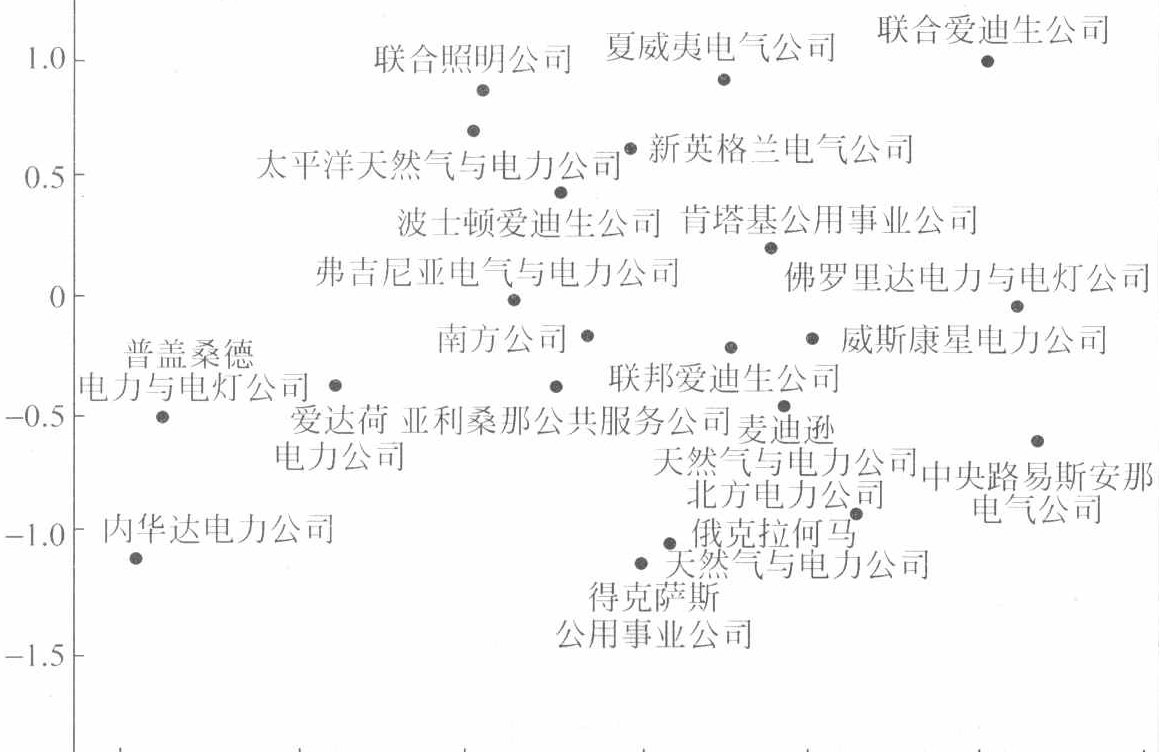
\includegraphics[width=98.2mm]{figs/fig_pg567_1.png}
\phantomsection\label{fig:12.18}\mvcap{图 12.18\quad 由多维标度变换产生的公用事业公司的几何表示}
\end{mvfigure}

虽然二维情形下的应力值相当高(应力$(2)\times 100\%=19\%$), \hyperref[fig:12.18]{图 12.18} 中诸公司间的距离与本章早些时候所提供的聚类分析结果差别不是特别大. 例如, 中西部的公司——联邦爱迪生、威斯康星电力(WEPCO)、麦迪逊天然气与电力(MG\&E), 以及北方电力(NSP)——彼此很接近(相似). 得克萨斯公用事业及俄克拉何马天然气与电力(Ok. G.\&E)也非常接近(相似). 其他公用事业公司倾向于按地理位置或相似的环境分组.

%% ===== pg-568 =====

% ---- pg-568 （书页 556） ----

这些公司在二维空间中布点后其点间距离 $d_{ik}^{(2)}$ 不可能与\hyperref[tab:12.6]{表 12.6} 中的原始(6 维)距离完全一致. 为了布点需要更大的灵活性, 而这种灵活性只有引进更多的维数才能得到.\hfill$\blacksquare$

\noindent\textbf{例 12.16}\quad (大学的多维标度变换)

\hyperref[tab:12.9]{表 12.9} 给出与 25 所美国大学有关的数据(见例 12.19). 这些数据中有: 新生入学的平均 SAT 得分, 新生在高中时排名前 $10\%$ 的人数百分比, 报考者的入学百分比, 学生教师比, 估计的年费用以及毕业率($\%$). 将度量多维标度变换算法用于经过标准化的大学数据, 便得到这些大学的二维表示, 结果示于\hyperref[fig:12.19]{图 12.19}. 注意私立大学在图的右边聚集, 而大型公立大学一般位于左侧.

\begin{mvfigure}
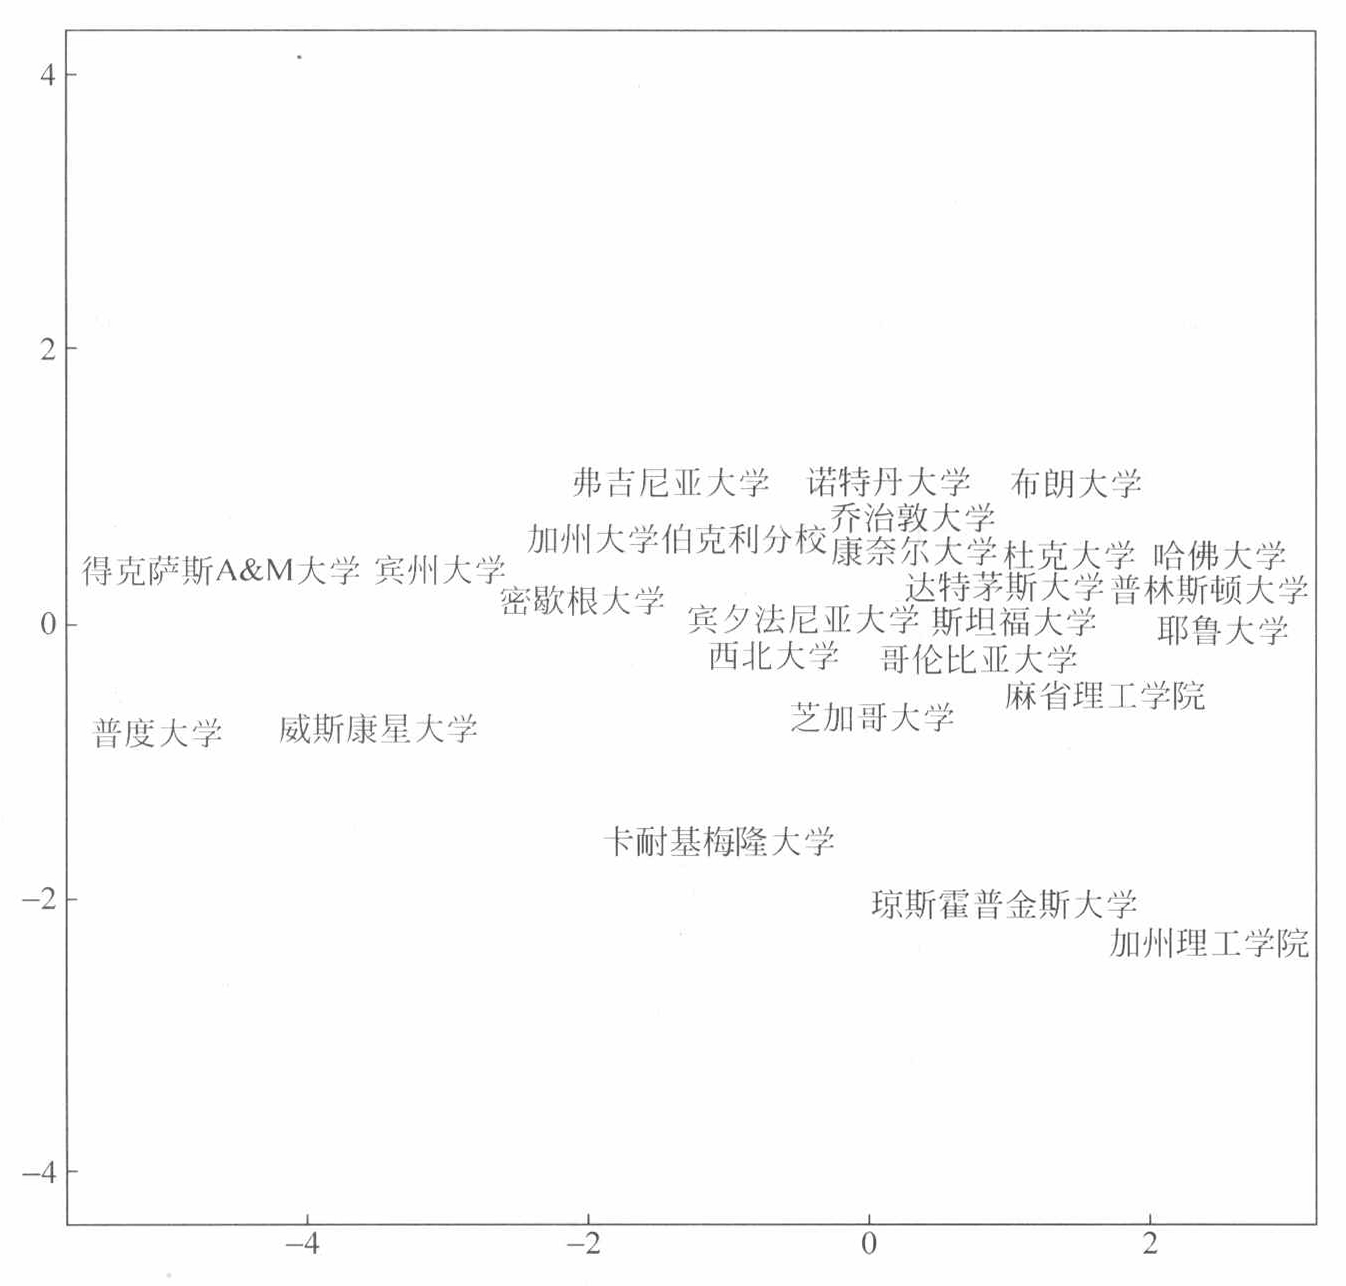
\includegraphics[width=114.0mm]{figs/fig_pg568_1.png}
\phantomsection\label{fig:12.19}\mvcap{图 12.19\quad 由度量多维标度变换得出的大学的二维表示}
\end{mvfigure}

对同一组数据用非度量多维标度变换得到的几何表示见\hyperref[fig:12.20]{图 12.20}. 对本例来说, 度量和非度量多维标度变换所给出的几何表示非常相似. 两种方法所给出的二维应力值都在 $10\%$ 左右.\hfill$\blacksquare$

经典的度量标度变换或主坐标分析, 等价于对主成分作图. 不同的软件程序选择特征向量的符号也不同, 因此初看起来两个解似乎是不同的. 然而, 如果对一个或两个坐标作镜面反射, 这两个解就完全一致(见文献[26]).

归纳起来, 多维标度变换法的关键目标是低维空间的图像. 无论何时, 只要多元数据可以表示为二维或三维空间中的图, 目测法就能对数据解释提供很大帮助.

当多元观测值有自然的数值, 且 $p$ 维空间中的欧氏距离 $d_{ik}^{(p)}$ 可以计算, 我们就可以通过使

%% ===== pg-569 =====

% ---- pg-569 （书页 557） ----

\begin{mvfigure}
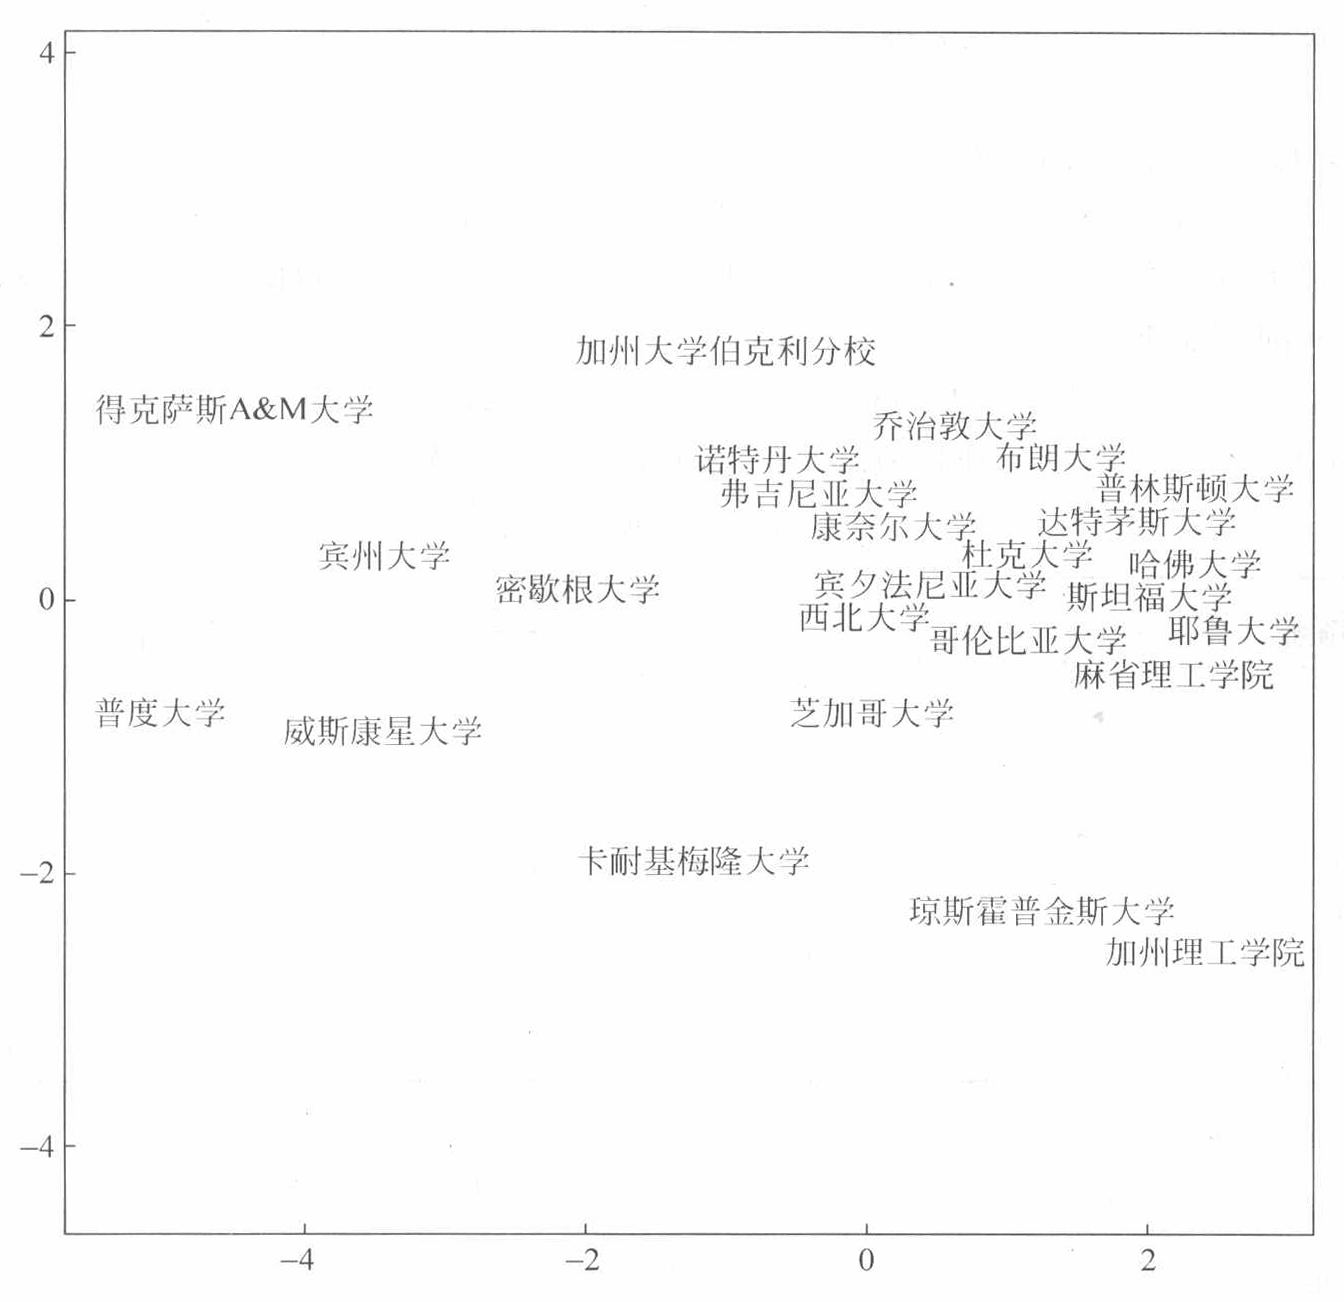
\includegraphics[width=113.8mm]{figs/fig_pg569_1.png}
\phantomsection\label{fig:12.20}\mvcap{图 12.20\quad 由非度量多维标度变换得出的大学的二维表示}
\end{mvfigure}

\phantomsection\label{eq:12-27}
\begin{equation}
E=\left[\sum_{i<k}\sum\left(d_{ik}^{(p)}-d_{ik}^{(q)}\right)^2\Big/d_{ik}^{(p)}\right]
\left[\sum_{i<k}\sum d_{ik}^{(p)}\right]^{-1}
\tag{12-27}
\end{equation}

达到最小来找到 $q<p$ 维表示. 在这种替代方法中, 将 $p$ 维和 $q$ 维欧氏距离进行直接比较. 通过使 $E$ 最小化来得到低维表示的方法称为非线性映射.

任一个低维表示的最后拟合优度均可用最小张树来表示(关于这个问题的进一步讨论见文献[16]).

\section{对应分析}
\phantomsection\label{sec:12.7}

对应分析是一种将频数或计数表中的各种联系用图来表示的方法, 由弗伦奇(French)所提出. 我们将集中讨论二维的频数表, 常称为列联表. 若列联表有 $I$ 行和 $J$ 列, 则由对应分析得出的图包含两组点, 一组有 $I$ 个点, 对应 $I$ 行; 另一组有 $J$ 个点, 对应 $J$ 列. 各点的位置反映各种联系.

相互接近的行点表明相应的行有相似的轮廓(条件分布). 相互接近的列点表明相应的列有相似的轮廓(条件分布). 最后, 行点和列点相互接近表明相应的组合发生的频数会高于独立模型(行类别与列类别之间没有关系的模型)下的期望值.

对应分析的输出包含数据的“最佳”二维表示、被标绘各点的坐标值以及每个维中所保留的信息量的一个度量(称为惯性).

%% ===== pg-570 =====

% ---- pg-570 （书页 558） ----

在扼要讨论对应分析的代数推导之前, 最好通过下面的一个例子来解释一下这种方法的基本思想.

\noindent\textbf{例 12.17}\quad (考古数据的对应分析)

\hyperref[tab:12.8]{表 12.8} 包含在美国西南部 $I=7$ 个考古场所挖掘出来的 $J=4$ 种不同类型陶器的频数. 表中行表示考古场所, 列表示陶器类型. 如果我们将每一行中的频数除以行的合计数, 就得到了在该场所的陶器类型的“轮廓”(条件分布). 对不同的场所(行), 陶器类型的轮廓用一个条形图示于\hyperref[fig:12.21]{图 12.21}(a). 条的宽度与行频数成比例. 一般来说, 对不同的行, 轮廓是不同的; 然而场所 P1 和场所 P2 的轮廓却相似. 同样, 场所 P4 和 P5 的轮廓也相似.

\begin{mvtable}
\phantomsection\label{tab:12.8}\mvtabcap{表 12.8\quad 陶器类型的频数}
\begin{tabular}{lccccc}
\toprule
\multirow{2}{*}{考古场所} & \multicolumn{4}{c}{陶器类型} & \multirow{2}{*}{合\quad 计} \\
\cmidrule(lr){2-5}
& A & B & C & D & \\
\midrule
P0 & 30 & 10 & 10 & 39 & 89 \\
P1 & 53 & 4 & 16 & 2 & 75 \\
P2 & 73 & 1 & 41 & 1 & 116 \\
P3 & 20 & 6 & 1 & 4 & 31 \\
P4 & 46 & 36 & 37 & 13 & 132 \\
P5 & 45 & 6 & 59 & 10 & 120 \\
P6 & 16 & 28 & 169 & 5 & 218 \\
\midrule
合\quad 计 & 283 & 91 & 333 & 74 & 781 \\
\bottomrule
\end{tabular}
\end{mvtable}

{\zihao{6}资料来源: 数据经 M.\,J.\,Tretter 许可使用.}

对不同类型的陶器(列), 考古场所的轮廓用条形图示于\hyperref[fig:12.21]{图 12.21}(b). 场所的轮廓用列合计数来构造. 图中各列的条形图看上去彼此不同. 这意味着各种类型的陶器在不同考古地点的分布是不同的.

\begin{mvfigure}
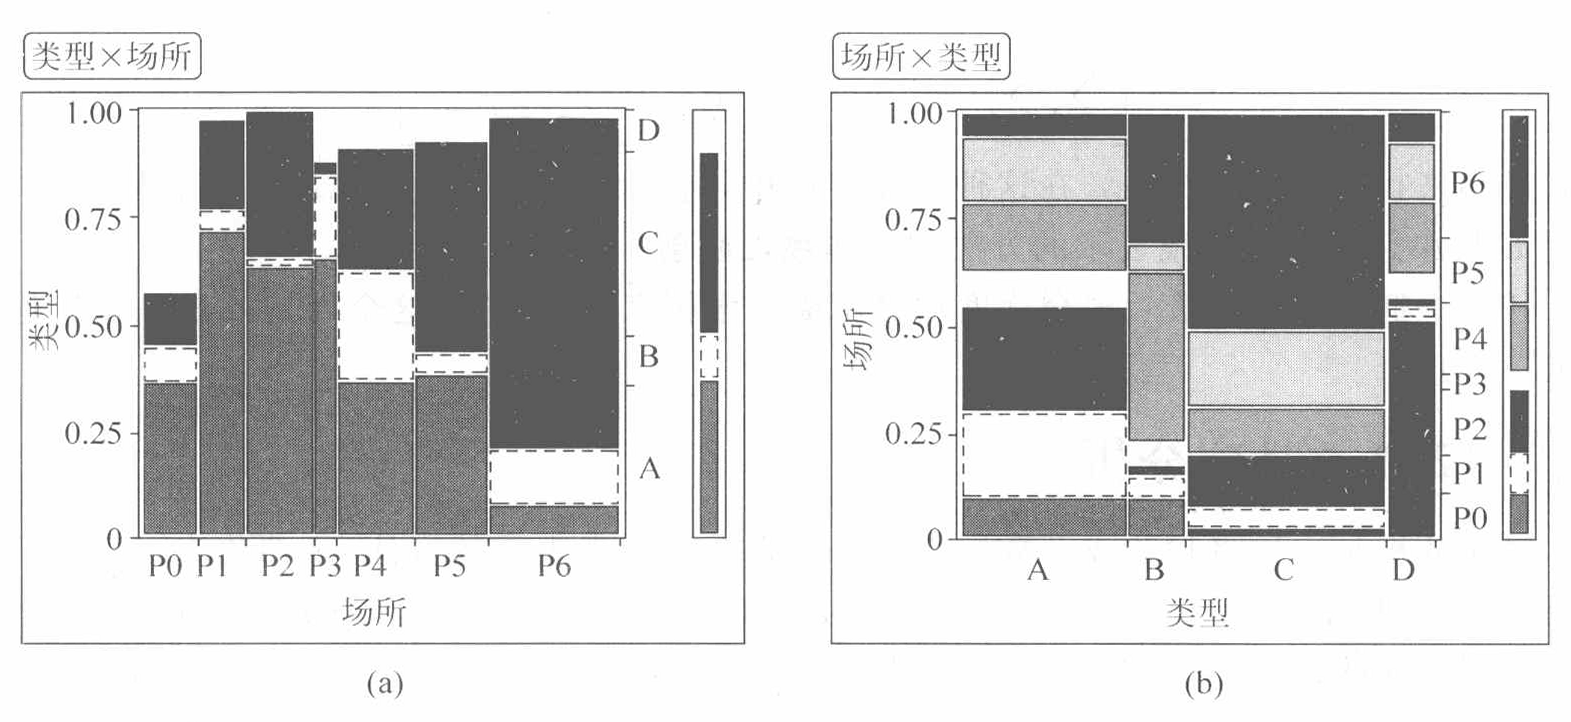
\includegraphics[width=133.0mm]{figs/fig_pg570_1.png}
\phantomsection\label{fig:12.21}\mvcap{图 12.21\quad 表 12.8 中数据的场所和陶器类型的轮廓}
\end{mvfigure}

对陶器类型—场所数据做对应分析\footnote{对\hyperref[tab:12.8]{表 12.8} 中的数据作对应分析时用了 JMP 软件.}得到的二维图示于\hyperref[fig:12.22]{图 12.22}.

%% ===== pg-571 =====

% ---- pg-571 （书页 559） ----

\begin{mvfigure}
\begin{tikzpicture}[x=2.6cm,y=2.6cm,font=\zihao{6}]
% ---- 边框 ----
\draw (-1.19,-1.08) rectangle (1.03,1.17);
% ---- 参考线 ----
\draw (-1.19,0) -- (1.03,0);
\draw (0,-1.08) -- (0,1.17);
% ---- x 轴主刻度 ----
\foreach \x in {-1.0,-0.5,0.0,0.5,1.0} \draw (\x,-1.08) -- (\x,-1.145);
% ---- x 轴次刻度 ----
\foreach \x in {-0.75,-0.25,0.25,0.75} \draw (\x,-1.08) -- (\x,-1.11);
\node[below,inner sep=1.5pt] at (-1.0,-1.145) {$-1.0$};
\node[below,inner sep=1.5pt] at (-0.5,-1.145) {$-0.5$};
\node[below,inner sep=1.5pt] at (0.0,-1.145) {$0.0$};
\node[below,inner sep=1.5pt] at (0.5,-1.145) {$0.5$};
\node[below,inner sep=1.5pt] at (1.0,-1.145) {$1.0$};
% ---- y 轴主刻度 ----
\foreach \y in {-1.0,-0.5,0.0,0.5,1.0} \draw (-1.19,\y) -- (-1.26,\y);
% ---- y 轴次刻度 ----
\foreach \y in {-0.75,-0.25,0.25,0.75} \draw (-1.19,\y) -- (-1.22,\y);
\node[left,inner sep=1.5pt] at (-1.26,1.0) {$1.0$};
\node[left,inner sep=1.5pt] at (-1.26,0.5) {$0.5$};
\node[left,inner sep=1.5pt] at (-1.26,0.0) {$0.0$};
\node[left,inner sep=1.5pt] at (-1.26,-0.5) {$-0.5$};
\node[left,inner sep=1.5pt] at (-1.26,-1.0) {$-1.0$};
% ---- 轴名 ----
\node[rotate=90,inner sep=1pt] at (-1.60,0) {$c_1$};
\node[below,inner sep=3pt] at (0,-1.42) {$c_2$};
% ---- 轴端注记 ----
\node[anchor=south west,inner sep=1pt] at (-1.19,1.20) {$\tilde{\lambda}_1^2=0.28(55\%)$};
\node[anchor=west,inner sep=1pt] at (1.05,0) {$\tilde{\lambda}_2^2=0.17(33\%)$};
% ---- 场所（空心方块） ----
\foreach \px/\py in {0.67/0.92, -0.64/0.42, -0.58/0.20, -0.28/0.72, 0.16/0.19, -0.15/0.00, 0.08/-0.61}
  \draw[fill=white] (\px-0.055,\py-0.055) rectangle (\px+0.055,\py+0.055);
% ---- 类型（实心方块 + 白色叉） ----
\foreach \px/\py in {-0.45/0.48, 0.32/0.00, -0.10/-0.43, 0.77/0.94} {
  \fill (\px-0.055,\py-0.055) rectangle (\px+0.055,\py+0.055);
  \draw[white,line width=0.4pt] (\px-0.055,\py-0.055) -- (\px+0.055,\py+0.055);
  \draw[white,line width=0.4pt] (\px-0.055,\py+0.055) -- (\px+0.055,\py-0.055);
}
% ---- 点标记 ----
\node[below,inner sep=2pt] at (0.67,0.92) {P0};
\node[below right,inner sep=2pt] at (-0.64,0.42) {P1};
\node[right,inner sep=2.5pt] at (-0.58,0.20) {P2};
\node[right,inner sep=2.5pt] at (-0.28,0.72) {P3};
\node[right,inner sep=2.5pt] at (0.16,0.19) {P4};
\node[left,inner sep=2.5pt] at (-0.15,0.00) {P5};
\node[right,inner sep=2.5pt] at (0.08,-0.61) {P6};
\node[right,inner sep=2.5pt] at (-0.45,0.48) {A};
\node[right,inner sep=2.5pt] at (0.32,0.00) {B};
\node[right,inner sep=2.5pt] at (-0.10,-0.43) {C};
\node[right,inner sep=2.5pt] at (0.77,0.94) {D};
% ---- 图例 ----
\begin{scope}[yshift=-4.5cm]
\fill (-0.80,-0.075) rectangle (-0.65,0.075);
\draw[white,line width=0.4pt] (-0.80,-0.075) -- (-0.65,0.075);
\draw[white,line width=0.4pt] (-0.80,0.075) -- (-0.65,-0.075);
\node[right,inner sep=3pt] at (-0.63,0) {类型};
\draw[fill=white] (0.10,-0.075) rectangle (0.25,0.075);
\node[right,inner sep=3pt] at (0.27,0) {场所};
\end{scope}
\end{tikzpicture}
\phantomsection\label{fig:12.22}\mvcap{图 12.22\quad 陶器类型—场所数据的对应分析图}
\end{mvfigure}

例如, \hyperref[fig:12.22]{图 12.22} 中的点指示场所 P1 和 P2 具有类似的陶器类型轮廓(两个点彼此靠近), 而场所 P0 和 P6 的轮廓则很不相同(两个点远离). 对应陶器类型的点散布得很开, 表示不同类型的考古地点的轮廓非常不同. 这些发现与\hyperref[fig:12.21]{图 12.21} 所画的轮廓是一致的.

注意点 P0 和 D 彼此很接近, 且与其他的点分开. 这说明 D 型陶器几乎是排他地与考古场所 P0 相联系. 类似的, 陶器类型 A 倾向于与场所 P1 相联系, 且较小程度上与 P2 和 P3 相联系. 陶器 B 与场所 P4 和 P5 相联系, 而类型 C 差不多只和场所 P6 相联系. 由于考古场所代表不同的年代, 这些联系对考古学家是有特别意义的.

位于二维图纵坐标轴末端的 $\tilde{\lambda}_1^2=0.28$ 是与第一维相联系的惯性, 这个惯性占总惯性的 $55\%$. 与第二维相联系的惯性为 $\tilde{\lambda}_2^2=0.17$, 占总惯性的 $33\%$. 两个维的惯性之和占总惯性的 $55\%+33\%=88\%$. 由于这个问题中的数据恰好可以用三维空间中的点来表示, \hyperref[fig:12.22]{图 12.22} 中的二维表示损失的信息(变差)很少. 等价地说, 我们可以认为这些点是多维行点集的“最佳”二维表示, 同时也是多维列点集的“最佳”二维表示. 总共 $88\%$ 的惯性说明这个表示对数据的“拟合”是好的.

在本例中, 对应分析的图像输出相当清晰地显示了列联表中各种联系的性质.\hfill$\blacksquare$

\mvsub{对应分析的代数推导}

首先, 令 $\mathbf{X}$ 为 $I\times J$ 列联表, 其元素 $x_{ij}$ 为未标准化的频数或计数. 在我们的讨论中, 总假定 $I>J$, 并且 $\mathbf{X}$ 满列秩. $\mathbf{X}$ 的行和列分别对应不同的类和不同的特性. 作为例子, \hyperref[tab:12.8]{表 12.8} 是一张列联表, 其中有 $I=7$ 个考古场所, $J=4$ 种陶器类型.

设 $n$ 为 $\mathbf{X}$ 中的总频数(译者注: $\mathbf{X}$ 中元素之和), 我们先构造比例矩阵 $\mathbf{P}=\{p_{ij}\}$, 其中
\phantomsection\label{eq:12-28}
\begin{equation}
p_{ij}=\frac{x_{ij}}{n},\quad i=1,\cdots,I,\ j=1,\cdots,J,\ \text{或}\
\underset{(I\times J)}{\mathbf{P}}=\frac{1}{n}\underset{(I\times J)}{\mathbf{X}}
\tag{12-28}
\end{equation}
矩阵 $\mathbf{P}$ 称为对应矩阵.

然后分别定义行和列的“和向量”$\mathbf{r}$ 和 $\mathbf{c}$:

%% ===== pg-572 =====

% ---- pg-572 （书页 560） ----

\phantomsection\label{eq:12-29}
\begin{equation}
\begin{aligned}
r_i&=\sum_{j=1}^{J}p_{ij}=\sum_{j=1}^{J}\frac{x_{ij}}{n},\quad i=1,\cdots,I,\ \text{或}\
\mathbf{r}=\underset{(I\times J)}{\mathbf{P}}\underset{(J\times 1)}{\mathbf{1}_J}\\
c_j&=\sum_{i=1}^{I}p_{ij}=\sum_{i=1}^{I}\frac{x_{ij}}{n},\quad j=1,\cdots,J,\ \text{或}\
\mathbf{c}=\underset{(J\times I)}{\mathbf{P}'}\underset{(I\times 1)}{\mathbf{1}_I}
\end{aligned}
\tag{12-29}
\end{equation}

其中 $\mathbf{1}_J$ 和 $\mathbf{1}_I$ 分布为所有元素为 1 的 $J\times 1$ 向量和 $I\times 1$ 向量. 定义对角矩阵
\phantomsection\label{eq:12-30}
\begin{equation}
\mathbf{D}_r=\operatorname{diag}(r_1,\cdots,r_I),\quad
\mathbf{D}_c=\operatorname{diag}(c_1,\cdots,c_J)
\tag{12-30}
\end{equation}
定义平方根矩阵
\phantomsection\label{eq:12-31}
\begin{equation}
\begin{aligned}
\mathbf{D}_r^{1/2}&=\operatorname{diag}(\sqrt{r_1},\cdots,\sqrt{r_I}),\quad
\mathbf{D}_r^{-1/2}=\operatorname{diag}\left(\frac{1}{\sqrt{r_1}},\cdots,\frac{1}{\sqrt{r_I}}\right)\\
\mathbf{D}_c^{1/2}&=\operatorname{diag}(\sqrt{c_1},\cdots,\sqrt{c_J}),\quad
\mathbf{D}_c^{-1/2}=\operatorname{diag}\left(\frac{1}{\sqrt{c_1}},\cdots,\frac{1}{\sqrt{c_J}}\right)
\end{aligned}
\tag{12-31}
\end{equation}

对应分析可以公式化为选择 $\hat{\mathbf{P}}=\{\hat{p}_{ij}\}$, 最小化加权平方和:
\phantomsection\label{eq:12-32}
\begin{equation}
\sum_{i=1}^{I}\sum_{j=1}^{J}\frac{(p_{ij}-\hat{p}_{ij})^2}{r_ic_j}
=\operatorname{tr}\left\{(\mathbf{D}_r^{-1/2}(\mathbf{P}-\hat{\mathbf{P}})\mathbf{D}_c^{-1/2})
(\mathbf{D}_r^{-1/2}(\mathbf{P}-\hat{\mathbf{P}})\mathbf{D}_c^{-1/2})'\right\}
\tag{12-32}
\end{equation}

注意: $(p_{ij}-\hat{p}_{ij})^2/\sqrt{r_ic_j}$ 是 $\mathbf{D}_r^{-1/2}(\mathbf{P}-\hat{\mathbf{P}})\mathbf{D}_c^{-1/2}$ 的 $(i,j)$ 元.

如结论 12.1 所证明, 对任意的 $I\times J$ 对应矩阵 $\mathbf{P}$, 其最佳逼近 $\hat{\mathbf{P}}$ 都包含 $\mathbf{r}\mathbf{c}'$, 且 $\mathbf{P}$ 的秩为 1 的最佳逼近为 $\hat{\mathbf{P}}=\mathbf{r}\mathbf{c}'$.

\mvthm{结论 12.1}{对任意的 $I\times J$ 对应矩阵 $\mathbf{P}$, 其最佳逼近 $\hat{\mathbf{P}}$ 都包含 $\mathbf{r}\mathbf{c}'$.}

$\mathbf{P}$ 的降秩到 $s$ 的最佳逼近(最小化\hyperref[eq:12-32]{式(12-32)}中的平方和)可表示成
\[
\mathbf{P}\doteq\sum_{k=1}^{s}\tilde{\lambda}_k(\mathbf{D}_r^{1/2}\tilde{\mathbf{u}}_k)(\mathbf{D}_c^{1/2}\tilde{\mathbf{v}}_k)'
=\mathbf{r}\mathbf{c}'+\sum_{k=2}^{s}\tilde{\lambda}_k(\mathbf{D}_r^{1/2}\tilde{\mathbf{u}}_k)(\mathbf{D}_c^{1/2}\tilde{\mathbf{v}}_k)'
\]
其中 $\tilde{\lambda}_k$ 为 $I\times J$ 矩阵 $\mathbf{D}_r^{-1/2}\mathbf{P}\mathbf{D}_c^{-1/2}$ 的奇异值, $I\times 1$ 向量 $\tilde{\mathbf{u}}_k$ 和 $J\times 1$ 向量 $\tilde{\mathbf{v}}_k$ 为对应的奇异向量.

\hyperref[eq:12-32]{式(12-32)}的最小值为 $\sum_{k=s+1}^{J}\tilde{\lambda}_k^2$.

$\mathbf{P}-\mathbf{r}\mathbf{c}'$ 的降秩到 $K>1$ 的逼近为
\phantomsection\label{eq:12-33}
\begin{equation}
\mathbf{P}-\mathbf{r}\mathbf{c}'\doteq\sum_{k=1}^{K}\lambda_k(\mathbf{D}_r^{1/2}\mathbf{u}_k)(\mathbf{D}_c^{1/2}\mathbf{v}_k)'
\tag{12-33}
\end{equation}
其中 $\lambda_k$ 为 $I\times J$ 矩阵 $\mathbf{D}_r^{-1/2}(\mathbf{P}-\mathbf{r}\mathbf{c}')\mathbf{D}_c^{-1/2}$ 的奇异值, $I\times 1$ 向量 $\mathbf{u}_k$ 和 $J\times 1$ 向量 $\mathbf{v}_k$ 为对应的奇异向量.

这里 $\lambda_k=\tilde{\lambda}_{k+1},\ \mathbf{u}_k=\tilde{\mathbf{u}}_{k+1},\ \mathbf{v}_k=\tilde{\mathbf{v}}_{k+1},\ k=1,\cdots,J-1$.

\mvbold{证明}\quad 我们首先考虑对应矩阵 $\mathbf{P}$ 的标准化形式 $\mathbf{D}_r^{-1/2}\mathbf{P}\mathbf{D}_c^{-1/2}$. $\mathbf{D}_r^{-1/2}\mathbf{P}\mathbf{D}_c^{-1/2}$ 的奇异值分解为
\phantomsection\label{eq:12-34}
\begin{equation}
\mathbf{D}_r^{-1/2}\mathbf{P}\mathbf{D}_c^{-1/2}=\sum_{k=1}^{J}\tilde{\lambda}_k\tilde{\mathbf{u}}_k\tilde{\mathbf{v}}_k'
\tag{12-34}
\end{equation}
其中
\phantomsection\label{eq:12-35}
\begin{equation}
\mathbf{D}_r^{-1/2}\mathbf{P}\mathbf{D}_c^{-1/2}\tilde{\mathbf{v}}_k=\tilde{\lambda}_k\tilde{\mathbf{u}}_k\qquad
\tilde{\mathbf{u}}_k'\mathbf{D}_r^{-1/2}\mathbf{P}\mathbf{D}_c^{-1/2}=\tilde{\lambda}_k\tilde{\mathbf{v}}_k'
\tag{12-35}
\end{equation}
且
\[
\left|(\mathbf{D}_r^{-1/2}\mathbf{P}\mathbf{D}_c^{-1/2})(\mathbf{D}_r^{-1/2}\mathbf{P}\mathbf{D}_c^{-1/2})'
-\tilde{\lambda}_k^2\mathbf{I}\right|=0,\quad k=1,\cdots,J
\]

%% ===== pg-573 =====

% ---- pg-573 （书页 561） ----

根据结论 2A.16, $\mathbf{D}_r^{-1/2}\mathbf{P}\mathbf{D}_c^{-1/2}$ 的最佳降秩到 $s$ 的逼近 $\hat{\mathbf{B}}$ 为奇异值分解的前 $s$ 项的和. 对 $\mathbf{P}$ 的逼近为
\[
\hat{\mathbf{P}}=\mathbf{D}_r^{1/2}\hat{\mathbf{B}}\mathbf{D}_c^{1/2}
=\sum_{k=1}^{s}\tilde{\lambda}_k(\mathbf{D}_r^{1/2}\tilde{\mathbf{u}}_k)(\mathbf{D}_c^{1/2}\tilde{\mathbf{v}}_k)'
\]
且根据结论 2A.16, 逼近的误差为 $\sum_{k=s+1}^{J}\tilde{\lambda}_k^2$.

对任意的 $I\times J$ 对应矩阵 $\mathbf{P}$, $\mathbf{r}\mathbf{c}'$ 总是其降秩到 1 的最佳逼近. 这结论等价于行和列的独立性假定. 为证明此结论, 令 $\tilde{\mathbf{u}}_1=\mathbf{D}_r^{-1/2}\mathbf{1}_I$, $\tilde{\mathbf{v}}_1=\mathbf{D}_c^{-1/2}\mathbf{1}_J$. 我们验证 $\tilde{\mathbf{u}}_1$ 和 $\tilde{\mathbf{v}}_1$ 满足\hyperref[eq:12-35]{式(12-35)}.
\[
\begin{aligned}
\tilde{\mathbf{u}}_1'(\mathbf{D}_r^{-1/2}\mathbf{P}\mathbf{D}_c^{-1/2})
&=(\mathbf{D}_r^{1/2}\mathbf{1}_I)'(\mathbf{D}_r^{-1/2}\mathbf{P}\mathbf{D}_c^{-1/2})\\
&=\mathbf{1}_I'\mathbf{P}\mathbf{D}_c^{-1/2}=\mathbf{c}'\mathbf{D}_c^{-1/2}\\
&=[\sqrt{c_1},\cdots,\sqrt{c_J}]=(\mathbf{D}_c^{1/2}\mathbf{1}_J)'=\tilde{\mathbf{v}}_1'
\end{aligned}
\]
并且
\[
\begin{aligned}
(\mathbf{D}_r^{-1/2}\mathbf{P}\mathbf{D}_c^{-1/2})\tilde{\mathbf{v}}_1
&=(\mathbf{D}_r^{-1/2}\mathbf{P}\mathbf{D}_c^{-1/2})(\mathbf{D}_c^{1/2}\mathbf{1}_J)\\
&=\mathbf{D}_r^{-1/2}\mathbf{P}\mathbf{1}_J=\mathbf{D}_r^{-1/2}\mathbf{r}\\
&=\begin{bmatrix}\sqrt{r_1}\\ \vdots\\ \sqrt{r_I}\end{bmatrix}
=\mathbf{D}_r^{1/2}\mathbf{1}_I=\tilde{\mathbf{u}}_1
\end{aligned}
\]
因此,
\phantomsection\label{eq:12-36}
\begin{equation}
(\tilde{\mathbf{u}}_1,\tilde{\mathbf{v}}_1)=(\mathbf{D}_r^{1/2}\mathbf{1}_I,\mathbf{D}_c^{1/2}\mathbf{1}_J)
\tag{12-36}
\end{equation}
为对应奇异值 $\tilde{\lambda}_1=1$ 的奇异向量. 对任意的对应矩阵 $\mathbf{P}$, 在任何展开中的公共项为
\[
\mathbf{D}_r^{1/2}\tilde{\mathbf{u}}_1\tilde{\mathbf{v}}_1'\mathbf{D}_c^{1/2}
=\mathbf{D}_r\mathbf{1}_I\mathbf{1}_J'\mathbf{D}_c=\mathbf{r}\mathbf{c}'
\]
这样, 我们建立了一阶逼近, 而\hyperref[eq:12-34]{式(12-34)}总可表示为
\[
\mathbf{P}=\mathbf{r}\mathbf{c}'+\sum_{k=2}^{J}\tilde{\lambda}_k(\mathbf{D}_r^{1/2}\tilde{\mathbf{u}}_k)(\mathbf{D}_c^{1/2}\tilde{\mathbf{v}}_k)'
\]
由于有公共项, 问题可转到 $\mathbf{P}-\mathbf{r}\mathbf{c}'$ 及其标准化 $\mathbf{D}_r^{-1/2}(\mathbf{P}-\mathbf{r}\mathbf{c}')\mathbf{D}_c^{-1/2}$. 由 $\mathbf{D}_r^{-1/2}\mathbf{P}\mathbf{D}_c^{-1/2}$ 的奇异向量间的正交性, 我们有 $\tilde{\mathbf{u}}_k'(\mathbf{D}_r^{1/2}\mathbf{1}_I)=0$ 及 $\tilde{\mathbf{v}}_k'(\mathbf{D}_c^{1/2}\mathbf{1}_J)=0, k>1$. 因此,
\[
\mathbf{D}_r^{-1/2}(\mathbf{P}-\mathbf{r}\mathbf{c}')\mathbf{D}_c^{-1/2}
=\sum_{k=2}^{J}\tilde{\lambda}_k\tilde{\mathbf{u}}_k\tilde{\mathbf{v}}_k'
\]
是以 $\mathbf{D}_r^{-1/2}\mathbf{P}\mathbf{D}_c^{-1/2}$ 的奇异值和奇异向量所表示的关于 $\mathbf{D}_r^{-1/2}(\mathbf{P}-\mathbf{r}\mathbf{c}')\mathbf{D}_c^{-1/2}$ 的奇异分解. 转化到 $\mathbf{D}_r^{-1/2}(\mathbf{P}-\mathbf{r}\mathbf{c}')\mathbf{D}_c^{-1/2}$ 本身的奇异值和奇异向量 $\lambda_k$, $\mathbf{u}_k$ 和 $\mathbf{v}_k$, 只需将 $k$ 变到 $k-1$. 因此 $\lambda_k=\tilde{\lambda}_{k+1}$, $\mathbf{u}_k=\tilde{\mathbf{u}}_{k+1}$, $\mathbf{v}_k=\tilde{\mathbf{v}}_{k+1}$, $k=1,\cdots,J-1$.

用 $\mathbf{D}_r^{-1/2}(\mathbf{P}-\mathbf{r}\mathbf{c}')\mathbf{D}_c^{-1/2}$ 的奇异分解得到 $\mathbf{P}-\mathbf{r}\mathbf{c}'$ 的展开
\phantomsection\label{eq:12-37}
\begin{equation}
\mathbf{P}-\mathbf{r}\mathbf{c}'=\sum_{k=1}^{J-1}\lambda_k(\mathbf{D}_r^{1/2}\mathbf{u}_k)(\mathbf{D}_c^{1/2}\mathbf{v}_k)'
\tag{12-37}
\end{equation}
由于 $\mathbf{D}_r^{-1/2}(\mathbf{P}-\mathbf{r}\mathbf{c}')\mathbf{D}_c^{-1/2}$ 的秩 $K$ 最佳逼近为 $\sum_{k=1}^{K}\tilde{\lambda}_k\tilde{\mathbf{u}}_k\tilde{\mathbf{v}}_k'$, 因此 $\mathbf{P}-\mathbf{r}\mathbf{c}'$ 的秩 $K$ 最佳逼近为
\phantomsection\label{eq:12-38}
\begin{equation}
\mathbf{P}-\mathbf{r}\mathbf{c}'\doteq\sum_{k=1}^{K}\lambda_k(\mathbf{D}_r^{1/2}\mathbf{u}_k)(\mathbf{D}_c^{1/2}\mathbf{v}_k)'
\tag{12-38}
\end{equation}
\hfill$\blacksquare$

%% ===== pg-574 =====

% ---- pg-574 （书页 562） ----

注: 虽然在\hyperref[eq:12-38]{式(12-38)}中向量 $\mathbf{D}_r^{1/2}\mathbf{u}_k$ 和 $\mathbf{D}_c^{1/2}\mathbf{v}_k$ 不必是单位长度的, 但是满足条件
\[
\begin{aligned}
(\mathbf{D}_r^{1/2}\mathbf{u}_k)'(\mathbf{D}_r^{1/2}\mathbf{u}_k)&=\mathbf{u}_k'\mathbf{u}_k=1\\
(\mathbf{D}_c^{1/2}\mathbf{v}_k)'(\mathbf{D}_c^{1/2}\mathbf{v}_k)&=\mathbf{v}_k'\mathbf{v}_k=1
\end{aligned}
\]
因此结论 12.1 中的展开称为广义奇异值分解.

令 $\boldsymbol{\Lambda}$, $\mathbf{U}=[\mathbf{u}_1,\cdots,\mathbf{u}_I]$ 和 $\mathbf{V}=[\mathbf{v}_1,\cdots,\mathbf{v}_J]$ 分别表示 $\mathbf{D}_r^{-1/2}(\mathbf{P}-\mathbf{r}\mathbf{c}')\mathbf{D}_c^{-1/2}$ 的奇异值矩阵和奇异向量矩阵. 在对应分析中, 通常将 $\mathbf{F}=\mathbf{D}_r^{-1}(\mathbf{D}_r^{1/2}\mathbf{U})\boldsymbol{\Lambda}$ 和 $\mathbf{G}=\mathbf{D}_c^{-1}(\mathbf{D}_c^{1/2}\mathbf{V})\boldsymbol{\Lambda}$ 的前两列或前三列用点图表示. $\mathbf{F}$ 和 $\mathbf{G}$ 的联合点图称为对称地图(symmetric map, 见文献[13]). 这是因为表示行和列的点在解的维度上有相同的标准化. 换句话说, 行点的几何与列点的几何一致.

\noindent\textbf{例 12.18}\quad (对应分析计算)

考虑如下的 $3\times 2$ 列联表

\begin{mvtable}
\begin{tabular}{lccc}
\toprule
& \textbf{B1} & \textbf{B2} & \textbf{和} \\
\midrule
\textbf{A1} & 24 & 12 & 36 \\
\textbf{A2} & 16 & 48 & 64 \\
\textbf{A3} & 60 & 40 & 100 \\
\midrule
\textbf{和} & 100 & 100 & 200 \\
\bottomrule
\end{tabular}
\end{mvtable}

对应矩阵为
\[
\mathbf{P}=\begin{bmatrix}0.12&0.06\\0.08&0.24\\0.30&0.20\end{bmatrix}
\]
列和向量 $\mathbf{c}'=[0.5,0.5]$, 行和向量 $\mathbf{r}'=[0.18,0.32,0.50]$. 负均方根矩阵
\[
\mathbf{D}_r^{-1/2}=\operatorname{diag}\left[\sqrt{2}/0.6,\sqrt{2}/0.8,\sqrt{2}\right],\quad
\mathbf{D}_c^{-1/2}=\operatorname{diag}\left[\sqrt{2},\sqrt{2}\right]
\]
由此,
\[
\mathbf{P}-\mathbf{r}\mathbf{c}'=
\begin{bmatrix}0.12&0.06\\0.08&0.24\\0.30&0.20\end{bmatrix}
-\begin{bmatrix}0.18\\0.32\\0.50\end{bmatrix}
\begin{bmatrix}0.5&0.5\end{bmatrix}
=\begin{bmatrix}0.03&-0.03\\-0.08&0.08\\0.05&-0.05\end{bmatrix}
\]
此矩阵的标准化为
\[
\begin{aligned}
\mathbf{A}&=\mathbf{D}_r^{-1/2}(\mathbf{P}-\mathbf{r}\mathbf{c}')\mathbf{D}_c^{-1/2}\\
&=\begin{bmatrix}\sqrt{2}/0.6&0&0\\0&\sqrt{2}/0.8&0\\0&0&\sqrt{2}\end{bmatrix}
\begin{bmatrix}0.03&-0.03\\-0.08&0.08\\0.05&-0.05\end{bmatrix}
\begin{bmatrix}\sqrt{2}&0\\0&\sqrt{2}\end{bmatrix}\\
&=\begin{bmatrix}0.1&-0.1\\-0.2&0.2\\0.1&-0.1\end{bmatrix}
\end{aligned}
\]
由于 $I>J$, 奇异值分解基于
\[
\mathbf{A}'\mathbf{A}=
\begin{bmatrix}0.1&-0.2&0.1\\-0.1&0.2&-0.1\end{bmatrix}
\begin{bmatrix}0.1&-0.1\\-0.2&0.2\\0.1&-0.1\end{bmatrix}
=\begin{bmatrix}0.06&-0.06\\-0.06&0.06\end{bmatrix}
\]
容易得到 $\tilde{\lambda}_1^2=0.12$, $\tilde{\lambda}_2^2=0$(由于 $J-1=2-1=1$). 对应奇异值 $\tilde{\lambda}_1$ 的列奇异向量

%% ===== pg-575 =====

% ---- pg-575 （书页 563） ----

\[
\mathbf{v}_1=\begin{bmatrix}1/\sqrt{2}\\-1/\sqrt{2}\end{bmatrix}
\]

进一步
\[
\mathbf{A}\mathbf{A}'=
\begin{bmatrix}0.1&-0.1\\-0.2&0.2\\0.1&-0.1\end{bmatrix}
\begin{bmatrix}0.1&-0.2&0.1\\-0.1&0.2&-0.1\end{bmatrix}
=\begin{bmatrix}0.02&-0.04&0.02\\-0.04&0.08&-0.04\\0.02&-0.04&0.02\end{bmatrix}
\]
计算机计算确认 $\lambda_1^2=0.12$, 因此 $\lambda_1=0.2\sqrt{3}$. 不难验证
\[
\mathbf{u}_1=\begin{bmatrix}1/\sqrt{6}\\-2/\sqrt{6}\\1/\sqrt{6}\end{bmatrix}
\]
由此得到 $\mathbf{P}-\mathbf{r}\mathbf{c}'$ 的单项展开
\[
\begin{aligned}
&\lambda_1(\mathbf{D}_r^{1/2}\mathbf{u}_1)(\mathbf{D}_c^{1/2}\mathbf{v}_1)'\\
&=\sqrt{0.12}
\begin{bmatrix}0.6/\sqrt{2}&0&0\\0&0.8/\sqrt{2}&0\\0&0&1/\sqrt{2}\end{bmatrix}
\begin{bmatrix}1/\sqrt{6}\\-2/\sqrt{6}\\1/\sqrt{6}\end{bmatrix}
\begin{bmatrix}1/\sqrt{2}&-1/\sqrt{2}\end{bmatrix}
\begin{bmatrix}1/\sqrt{2}&0\\0&1/\sqrt{2}\end{bmatrix}\\
&=\sqrt{0.12}
\begin{bmatrix}0.3/\sqrt{3}\\-0.8/\sqrt{3}\\0.5/\sqrt{3}\end{bmatrix}
\begin{bmatrix}1/2&-1/2\end{bmatrix}
=\begin{bmatrix}0.03&-0.03\\-0.08&0.08\\0.05&-0.05\end{bmatrix}
\end{aligned}
\]
这里只有一对向量供布点:
\[
\lambda_1\mathbf{D}_r^{1/2}\mathbf{u}_1=\sqrt{0.12}
\begin{bmatrix}0.6/\sqrt{2}&0&0\\0&0.8/\sqrt{2}&0\\0&0&1/\sqrt{2}\end{bmatrix}
\begin{bmatrix}1/\sqrt{6}\\-2/\sqrt{6}\\1/\sqrt{6}\end{bmatrix}
=\sqrt{0.12}\begin{bmatrix}0.3/\sqrt{3}\\-0.8/\sqrt{3}\\0.5/\sqrt{3}\end{bmatrix}
\]
\[
\lambda_1\mathbf{D}_c^{1/2}\mathbf{v}_1=\sqrt{0.12}
\begin{bmatrix}1/\sqrt{2}&0\\0&1/\sqrt{2}\end{bmatrix}
\begin{bmatrix}\frac{1}{\sqrt{2}}&-\frac{1}{\sqrt{2}}\end{bmatrix}
=\sqrt{0.12}\begin{bmatrix}1/2\\-1/2\end{bmatrix}
\]
\hfill$\blacksquare$

还有第二种方法定义列联表分析. 遵循格里纳克(Greenacre, 见文献[13]), 我们称前述方法为矩阵逼近法, 而下面要介绍的方法为轮廓逼近法. 我们对(列联表的)行作轮廓逼近的解释. 当然, 对列也可以作相似的轮廓逼近.

在代数的意义上, 行轮廓是矩阵 $\mathbf{D}_r^{-1}\mathbf{P}$ 的行. 因此列联表分析可定义为用低维空间中的点逼近行轮廓. 考虑用矩阵 $\mathbf{P}^*$ 逼近行轮廓. 用\hyperref[eq:12-31]{式(12-31)}中定义的平方根矩阵 $\mathbf{D}_r^{1/2}$ 和 $\mathbf{D}_c^{1/2}$, 我们有
\[
(\mathbf{D}_r^{-1}\mathbf{P}-\mathbf{P}^*)\mathbf{D}_c^{-1/2}
=\mathbf{D}_r^{-1/2}(\mathbf{D}_r^{-1/2}\mathbf{P}-\mathbf{D}_r^{1/2}\mathbf{P}^*)\mathbf{D}_c^{-1/2}
\]
令 $p_{ij}^*=\hat{p}_{ij}/r_i$, 均方准则(12-32)可以写成
\phantomsection\label{eq:12-39}
\begin{equation}
\begin{aligned}
&\sum_{i=1}^{I}\sum_{j=1}^{J}\frac{(p_{ij}-\hat{p}_{ij})^2}{r_ic_j}\\
&\quad=\sum_{i=1}^{I}\sum_{j=1}^{J}\frac{(p_{ij}/r_i-p_{ij}^*)^2}{c_j}\\
&\quad=\operatorname{tr}\left\{\mathbf{D}_r^{1/2}\mathbf{D}_r^{1/2}(\mathbf{D}_r^{-1}\mathbf{P}-\mathbf{P}^*)
\mathbf{D}_c^{-1/2}\mathbf{D}_c^{-1/2}(\mathbf{D}_r^{-1}\mathbf{P}-\mathbf{P}^*)'\right\}\\
&\quad=\operatorname{tr}\left\{\mathbf{D}_r^{1/2}(\mathbf{D}_r^{-1/2}\mathbf{P}-\mathbf{D}_r^{-1/2}\mathbf{P}^*)
\mathbf{D}_c^{-1/2}\mathbf{D}_c^{-1/2}(\mathbf{D}_r^{-1/2}\mathbf{P}-\mathbf{D}_r^{-1/2}\mathbf{P}^*)'\mathbf{D}_r^{-1/2}\right\}\\
&\quad=\operatorname{tr}\left\{[(\mathbf{D}_r^{-1/2}\mathbf{P}-\mathbf{D}_r^{-1/2}\mathbf{P}^*)\mathbf{D}_c^{-1/2}]
[(\mathbf{D}_r^{-1/2}\mathbf{P}-\mathbf{D}_r^{-1/2}\mathbf{P}^*)\mathbf{D}_c^{-1/2}]'\right\}
\end{aligned}
\tag{12-39}
\end{equation}

%% ===== pg-576 =====

% ---- pg-576 （书页 564） ----

最小化\hyperref[eq:12-39]{式(12-39)}右端的“迹”恰好是在结论 12.1 的证明中的第一个最小化问题. 由\hyperref[eq:12-34]{式(12-34)}, $\mathbf{D}_r^{-1/2}\mathbf{P}\mathbf{D}_c^{-1/2}$ 有奇异值分解
\phantomsection\label{eq:12-40}
\begin{equation}
\mathbf{D}_r^{-1/2}\mathbf{P}\mathbf{D}_c^{-1/2}=\sum_{k=1}^{J}\tilde{\lambda}_k\tilde{\mathbf{u}}_k\tilde{\mathbf{v}}_k'
\tag{12-40}
\end{equation}
最佳秩 $K$ 逼近可用此展开式的前 $K$ 项表示. 由\hyperref[eq:12-39]{式(12-39)}, 由于 $\mathbf{D}_r^{-1/2}\mathbf{P}\mathbf{D}_c^{-1/2}$ 可用 $\mathbf{D}_r^{-1/2}\mathbf{P}^*\mathbf{D}_c^{-1/2}$ 逼近, 对\hyperref[eq:12-40]{式(12-40)}左乘 $\mathbf{D}_r^{-1/2}$, 右乘 $\mathbf{D}_c^{1/2}$, 得到广义奇异值分解
\phantomsection\label{eq:12-41}
\begin{equation}
\mathbf{D}_r^{-1}\mathbf{P}=\sum_{k=1}^{J}\tilde{\lambda}_k\mathbf{D}_r^{-1/2}\tilde{\mathbf{u}}_k
(\mathbf{D}_c^{-1/2}\tilde{\mathbf{v}}_k)'
\tag{12-41}
\end{equation}
其中, 根据\hyperref[eq:12-36]{式(12-36)}, $(\tilde{\mathbf{u}}_1,\tilde{\mathbf{v}}_1)=(\mathbf{D}_r^{1/2}\mathbf{1}_I,\mathbf{D}_c^{1/2}\mathbf{1}_J)$ 为关联于奇异值 $\tilde{\lambda}_1=1$ 的奇异向量. 由于 $\mathbf{D}_r^{-1/2}(\mathbf{D}_r^{1/2}\mathbf{1}_I)=\mathbf{1}_I$ 且 $(\mathbf{D}_c^{1/2}\mathbf{1}_J)'\mathbf{D}_c^{-1/2}=\mathbf{c}'$, 在\hyperref[eq:12-41]{式(12-41)}中, 第一项为 $\mathbf{1}_I\mathbf{c}'$.

因此, 基于 $\mathbf{D}_r^{-1/2}\mathbf{P}\mathbf{D}_c^{-1/2}$ 的奇异值和奇异向量, 行轮廓 $\mathbf{D}_r^{-1}\mathbf{P}$ 的秩 $K(<J)$ 逼近为
\phantomsection\label{eq:12-42}
\begin{equation}
\mathbf{P}^*\doteq\mathbf{1}_I\mathbf{c}'+\sum_{k=2}^{K}\tilde{\lambda}_k\mathbf{D}_r^{-1/2}\tilde{\mathbf{u}}_k
(\mathbf{D}_c^{-1/2}\tilde{\mathbf{v}}_k)'
\tag{12-42}
\end{equation}
基于 $\mathbf{D}_r^{-1/2}(\mathbf{P}-\mathbf{r}\mathbf{c}')\mathbf{D}_c^{-1/2}$ 的奇异值和奇异向量 $\lambda_k$, $\mathbf{u}_k$ 和 $\mathbf{v}_k$, 我们有
\[
\mathbf{P}^*-\mathbf{1}_I\mathbf{c}'\doteq\sum_{k=1}^{K-1}\lambda_k\mathbf{D}_r^{-1/2}\mathbf{u}_k
(\mathbf{D}_c^{-1/2}\mathbf{v}_k)'
\]
(对\hyperref[tab:12.8]{表 12.8} 中的考古数据的行轮廓分析结果显示在\hyperref[fig:12.21]{图 12.21} 中.)

\mvsub{惯性}

总惯性是数据总变差的度量, 定义为加权平方和
\phantomsection\label{eq:12-43}
\begin{equation}
\operatorname{tr}\left\{\mathbf{D}_r^{-1/2}(\mathbf{P}-\mathbf{r}\mathbf{c}')\mathbf{D}_c^{-1/2}
\left[\mathbf{D}_r^{-1/2}(\mathbf{P}-\mathbf{r}\mathbf{c}')\mathbf{D}_c^{-1/2}\right]'\right\}
=\sum_{i}\sum_{j}\frac{(p_{ij}-r_ic_j)^2}{r_ic_j}=\sum_{k=1}^{J-1}\lambda_k^2
\tag{12-43}
\end{equation}
其中 $\lambda_k$ 为 $\mathbf{D}_r^{-1/2}(\mathbf{P}-\mathbf{r}\mathbf{c}')\mathbf{D}_c^{-1/2}$ 的奇异值(见结论 12.1 的证明).\textsuperscript{①}

对于中心化的矩阵 $\mathbf{P}-\mathbf{r}\mathbf{c}'$, 最佳秩 $K(<J)$ 逼近($K$ 维解)具有惯性 $\sum_{k=1}^{K}\lambda_k^2$. 剩余惯性等于剩余奇异值的平方和 $\sum_{k=K+1}^{J-1}\lambda_k^2$. 在布点时, 第 $k$ 维的坐标以平方根惯性 $\lambda_k$ 为尺度, 如\hyperref[fig:12.22]{图 12.22} 所示(译者注: 此句是根据译者理解的意译, 原文的直译难以理解).

\mvsub{二维空间中的解释}

由于惯性是数据总变差的度量, 对于大的 $(\lambda_1^2+\lambda_2^2)\big/\sum_{k=1}^{J-1}\lambda_k^2$, 我们如何解释? 从几何的意义上, 我们可以说: 中心化的数据可以用平面上的点来表示. 并且, 在秩 1 解(独立模型)之外, 这个最佳逼近平面解释了几平所有的变差. 从代数的意义上, 我们说秩 2 逼近
\[
\mathbf{P}-\mathbf{r}\mathbf{c}'\doteq\lambda_1\mathbf{u}_1\mathbf{v}_1'+\lambda_2\mathbf{u}_2\mathbf{v}_2'
\]
是很好的逼近, 或者说
\[
\mathbf{P}\doteq\mathbf{r}\mathbf{c}'+\lambda_1\mathbf{u}_1\mathbf{v}_1'+\lambda_2\mathbf{u}_2\mathbf{v}_2'
\]

\vspace{6pt}
\noindent\rule{\linewidth}{0.4pt}
\par\vspace{2pt}
{\zihao{6}①\quad 总惯性与二维列联表的卡方度量
$\chi^2=\sum\limits_{i,j}\frac{(O_{ij}-E_{ij})^2}{E_{ij}}$ 有关. 这里 $O_{ij}=x_{ij}$ 为观测的频数,
$E_{ij}$ 为期望频数. 在我们的讨论中, 若行变量独立(不相关)于列变量, 则 $E_{ij}=nr_ic_j$, 因此
\[
\text{总惯性}=\sum_{i=1}^{I}\sum_{j=1}^{J}\frac{(p_{ij}-r_ic_j)^2}{r_ic_j}=\frac{1}{n}\chi^2
\]}

%% ===== pg-577 =====

% ---- pg-577 （书页 565） ----

\mvsub{最后评论}

对应分析本质上是一种图方法, 用于表示在低维空间中变量间的关系. 此方法可以看做是一种标度方法, 因此可以看做是其他方法如多维标度法(12.6 节)或双重信息法(12.8 节)的补充. 对应分析与主成分分析(第 10 章)和正则相关分析(第 10 章)有联系. 欲了解更多有关对应分析的知识, 可阅读格里纳克的书(见文献[14]).

\section{用于观察抽样单元和变量的双重信息图}
\phantomsection\label{sec:12.8}

双重信息图是 $n\times p$ 数据集中信息的一种图形表示方法. “双重”是指包含在数据集中的两类信息: 行中的信息属于样本或抽样单元, 而列中的信息则属于变量.

当只有两个变量时, 通过散布图就能将抽样单元中的信息和变量中的信息在同一张图上表示出来. 这样人们就可以通过视觉来检查一个抽样单元相对另一个抽样单元的位置, 以及两个变量中的每一个与任一个单元位置的相对重要性.

当存在若干个变量时, 我们可以构造散布图矩阵, 但不能将抽样单元表示在一张图上. 另一方面, 抽样单元的二维图可以通过对前两个主成分作图来得到(见 8.4 节). 隐藏在双重信息图背后的想法是将有关变量的信息加到主成分图中去.

\hyperref[fig:12.23]{图 12.23} 给出\hyperref[tab:12.4]{表 12.4} 中公用事业公司数据的双重信息图. 从图中可以看出公司之间是如何分组聚类的, 以及变量对它们位置的贡献. 例如, 变量 $X_4$(=年载荷因子)和 $X_8$(=总燃料成本)基本上将大部分沿海公司集中在图的右下角. 变量 $X_1$(=固定费用比)和 $X_2$(=资本回报率)将佛罗里达和路易斯安那的公司聚集在一起.

\begin{mvfigure}
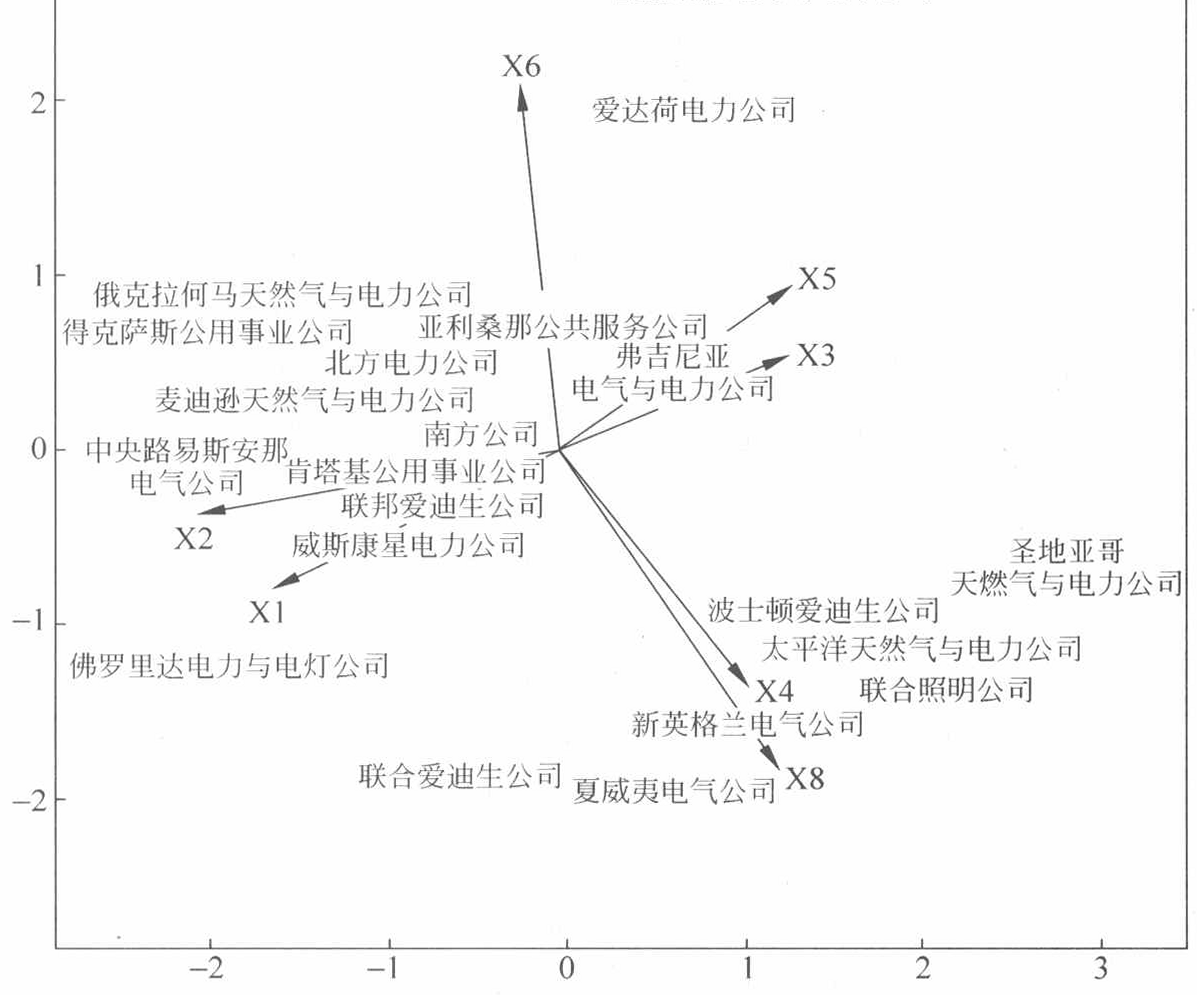
\includegraphics[width=101.4mm]{figs/fig_pg577_1.png}
\phantomsection\label{fig:12.23}\mvcap{图 12.23\quad 公用事业公司数据的双重信息图}
\end{mvfigure}

%% ===== pg-578 =====

% ---- pg-578 （书页 566） ----

\mvsub{构造双重信息图}

双重信息图的构造由样本主成分开始.

根据结论 8A.1, 数据阵 $\mathbf{X}$ 的最佳二维近似用前两个主成分的样本值来逼近第 $j$ 个观测值 $\mathbf{x}_j$. 具体说就是
\phantomsection\label{eq:12-44}
\begin{equation}
\mathbf{x}_j\doteq\bar{\mathbf{x}}+\hat{y}_{j1}\hat{\mathbf{e}}_1+\hat{y}_{j2}\hat{\mathbf{e}}_2
\tag{12-44}
\end{equation}
其中 $\hat{\mathbf{e}}_1$ 和 $\hat{\mathbf{e}}_2$ 为 $\mathbf{S}$ 或 $\mathbf{X}_c'\mathbf{X}_c=(n-1)\mathbf{S}$ 的前两个特征向量. 这里 $\mathbf{X}_c$ 为修正的数据阵, 其行为 $(\mathbf{x}_j-\bar{\mathbf{x}})'$. 这两个特征向量确定一个平面, 第 $j$ 个抽样单元(行)在该平面上的坐标为一对主成分值 $(\hat{y}_{j1},\hat{y}_{j2})$.

为了将关于变量的信息也包括到这个平面图中, 我们考虑一对特征向量 $(\hat{\mathbf{e}}_1,\hat{\mathbf{e}}_2)$. 这两个特征向量是前两个样本主成分的系数向量. 因此, 矩阵 $\hat{\mathbf{E}}=[\hat{\mathbf{e}}_1,\hat{\mathbf{e}}_2]$ 的每一行确定一个变量在图中的位置, 而系数的大小(变量的坐标)则给出相应变量在主成分中的权值. 变量在图中的位置用一个向量来指示. 通常, 统计计算机程序会给出一个乘子, 将所有向量的长度作适当调整并像抽样单元那样标绘在同一坐标系上. 同某个变量比较接近的那些单元很可能在那个变量上有较大的值. 为解释一个新点 $\mathbf{x}_0$, 我们在图中对它的主成分 $\hat{\mathbf{E}}'(\mathbf{x}_0-\bar{\mathbf{x}})$ 作出标绘.

一种直接得出双重信息图的方法是从奇异值分解开始(见结论 2A.15). 首先将 $n\times p$ 均值修正矩阵 $\mathbf{X}_c$ 表示为
\phantomsection\label{eq:12-45}
\begin{equation}
\underset{n\times p}{\mathbf{X}_c}=\underset{(n\times p)}{\mathbf{U}}
\underset{(p\times p)}{\boldsymbol{\Delta}}\underset{(p\times p)}{\mathbf{V}'}
\tag{12-45}
\end{equation}
其中 $\boldsymbol{\Delta}$ 为对角 $(\lambda_1,\lambda_2,\cdots,\lambda_p)$, 且 $\mathbf{V}$ 为一个正交阵, 其列向量为 $\mathbf{X}_c'\mathbf{X}_c=(n-1)\mathbf{S}$ 的特征向量. 也就是说, $\mathbf{V}=\hat{\mathbf{E}}=[\hat{\mathbf{e}}_1,\hat{\mathbf{e}}_2,\cdots,\hat{\mathbf{e}}_p]$. 将\hyperref[eq:12-45]{式(12-45)}的右端乘以 $\hat{\mathbf{E}}$, 我们有
\phantomsection\label{eq:12-46}
\begin{equation}
\mathbf{X}_c\hat{\mathbf{E}}=\mathbf{U}\boldsymbol{\Delta}
\tag{12-46}
\end{equation}
此等式左端矩阵的第 $j$ 行
\[
\left[(\mathbf{x}_j-\bar{\mathbf{x}})'\hat{\mathbf{e}}_1,(\mathbf{x}_j-\bar{\mathbf{x}})'\hat{\mathbf{e}}_2,\cdots,
(\mathbf{x}_j-\bar{\mathbf{x}})'\hat{\mathbf{e}}_p\right]=[\hat{y}_{j1},\hat{y}_{j2},\cdots,\hat{y}_{jp}]
\]
恰好是第 $j$ 个单元的主成分值. 也就是说, $\mathbf{U}\boldsymbol{\Delta}$ 包含所有的主成分值, 而 $\mathbf{V}=\hat{\mathbf{E}}$ 则包含定义主成分的那些系数.

$\mathbf{X}_c$ 的最佳二维近似可以用 $\boldsymbol{\Delta}^*=\text{对角}(\lambda_1,\lambda_2,0,\cdots,0)$ 代替 $\boldsymbol{\Delta}$ 得到. 这个结果称为埃卡尔特-扬(Eckart-Young)定理. 证明在结论 8A.1 中. 于是(最佳二维)近似为
\phantomsection\label{eq:12-47}
\begin{equation}
\mathbf{X}_c\doteq\mathbf{U}\boldsymbol{\Delta}^*\mathbf{V}'
=[\hat{\mathbf{y}}_1,\hat{\mathbf{y}}_2]\begin{bmatrix}\hat{\mathbf{e}}_1'\\ \hat{\mathbf{e}}_2'\end{bmatrix}
\tag{12-47}
\end{equation}
其中 $\hat{\mathbf{y}}_1$ 和 $\hat{\mathbf{y}}_2$ 分别为前两个主成分的值的 $n\times 1$ 向量.

在双重信息图中, 数据矩阵的每一行(或项目)用一个点表示, 其位置由两个主成分的一对值决定. 数据矩阵的第 $i$ 列(或变量)用一个从原点引出指向该点的箭头表示, 箭头端点的坐标为 $(e_{1i},e_{2i})$——\hyperref[eq:12-47]{式(12-47)}右端第二个矩阵 $[\hat{\mathbf{e}}_1,\hat{\mathbf{e}}_2]'$ 第 $i$ 列中的元素. 这个尺度与主成分的尺度也许不相匹配, 所以引进一个任意乘子, 以同一个量将所有向量进行调整.

双重信息图的思想(即同时将抽样单元和变量表示在一个图中)可推广到正则相关分析和多维标度变换, 甚至可推广到更复杂的非线性方法(见文献[12]).

%% ===== pg-579 =====

% ---- pg-579 （书页 567） ----

\noindent\textbf{例 12.19}\quad (大学及其特征的双重信息图)

\hyperref[tab:12.9]{表 12.9} 给出某些大学对一些变量的数据, 用于将主要大学进行比较或排队. 这些变量包括 $X_1$=新生的平均 SAT 得分, $X_2$=新生在高中时期名列班上 前 $10\%$ 的人数百分比, $X_3$=报名者被接受入学的百分比, $X_4$=学生与教师的比例, $X_5$=估计的年费用, 及 $X_6$=毕业比例($\%$).

\begin{mvtable}
\phantomsection\label{tab:12.9}\mvtabcap{表 12.9\quad 大学数据}
\setlength{\tabcolsep}{3.5pt}%
\zihao{6}%
\begin{longtable}{lrrrrrr}\toprule
\textbf{大\quad 学} & $X_1$ & $X_2$ & $X_3$ & $X_4$ & $X_5$ & $X_6$ \\
\midrule
\endfirsthead
\multicolumn{7}{c}{\zihao{6}续表}\\
\toprule
\textbf{大\quad 学} & $X_1$ & $X_2$ & $X_3$ & $X_4$ & $X_5$ & $X_6$ \\
\midrule
\endhead
\bottomrule
\endlastfoot

哈佛大学(Harvard) & 14.00 & 91 & 14 & 11 & 39{,}525 & 97 \\
普林斯顿大学(Princeton) & 13.75 & 91 & 14 & 8 & 30{,}220 & 95 \\
耶鲁大学(Yale) & 13.75 & 95 & 19 & 11 & 43{,}514 & 96 \\
斯坦福大学(Stanford) & 13.60 & 90 & 20 & 12 & 36{,}450 & 93 \\
麻省理工学院(MIT) & 13.80 & 94 & 30 & 10 & 34{,}870 & 91 \\
杜克大学(Duke) & 13.15 & 90 & 30 & 12 & 31{,}585 & 95 \\
加州理工学院(CalTech) & 14.15 & 100 & 25 & 6 & 63{,}575 & 81 \\
达特茅斯大学(Dartmouth) & 13.40 & 89 & 23 & 10 & 32{,}162 & 95 \\
布朗大学(Brown) & 13.10 & 89 & 22 & 13 & 22{,}704 & 94 \\
琼斯霍普金斯大学(JohnsHopkins) & 13.05 & 75 & 44 & 7 & 58{,}691 & 87 \\
芝加哥大学(UChicago) & 12.90 & 75 & 50 & 13 & 38{,}380 & 87 \\
宾夕法尼亚大学(UPenn) & 12.85 & 80 & 36 & 11 & 27{,}553 & 90 \\
康奈尔大学(Cornell) & 12.80 & 83 & 33 & 13 & 21{,}864 & 90 \\
西北大学(Northwestern) & 12.60 & 85 & 39 & 11 & 28{,}052 & 89 \\
哥伦比亚大学(Columbia) & 13.10 & 76 & 24 & 12 & 31{,}510 & 88 \\
诺特丹大学(NotreDame) & 12.55 & 81 & 42 & 13 & 15{,}122 & 94 \\
弗吉尼亚大学(UVirginia) & 12.25 & 77 & 44 & 14 & 13{,}349 & 92 \\
乔治敦大学(Georgetown) & 12.55 & 74 & 24 & 12 & 20{,}126 & 92 \\
卡耐基梅隆大学(CarnegieMellon) & 12.60 & 62 & 59 & 9 & 25{,}026 & 72 \\
密歇根大学(UMichigan) & 11.80 & 65 & 68 & 16 & 15{,}470 & 85 \\
加州大学(伯克利分校)(UCBerkeley) & 12.40 & 95 & 40 & 17 & 15{,}140 & 78 \\
威斯康星大学(UWisconsin) & 10.85 & 40 & 69 & 15 & 11{,}857 & 71 \\
宾州大学(PennState) & 10.81 & 38 & 54 & 18 & 10{,}185 & 80 \\
普度大学(Purdue) & 10.05 & 28 & 90 & 19 & 9{,}066 & 69 \\
得克萨斯 A\&M 大学(TexasA\&M) & 10.75 & 49 & 67 & 25 & 8{,}704 & 67 \\
\end{longtable}
\end{mvtable}

{\zihao{6}资料来源: 美国新闻与世界报道, 1995 年 9 月 18 日.}

由于其中两个变量(SAT 得分和费用)在尺度上与其他变量有很大差别, 我们将数据标准化, 并根据标准化观测值 $\mathbf{z}_j$ 的矩阵作双重信息图. 这个双重信息图在\hyperref[fig:12.24]{图 12.24} 中给出.

注意加州理工学院和琼斯霍普金斯大学远离群体单独在一起, 费用变量($X_5$)对这种定位负主要责任. 在我们的样本中, 大型州立大学在图的左侧, 而大部分私立大学集中在图的右侧. 变量 SAT($X_1$)、前 10 名比例($X_2$)和毕业率($X_6$)的较大值是与私立学校组相联系的. 西北大学位于图的中心.\hfill$\blacksquare$

高尔和韩德(Gower \& Hand, 见文献[12])开发了一种新的双重信息图方法, 有某些优点. 他们的方法是对散点图的推广, 具有易于解释的特点:

%% ===== pg-580 =====

% ---- pg-580 （书页 568） ----

\begin{mvfigure}
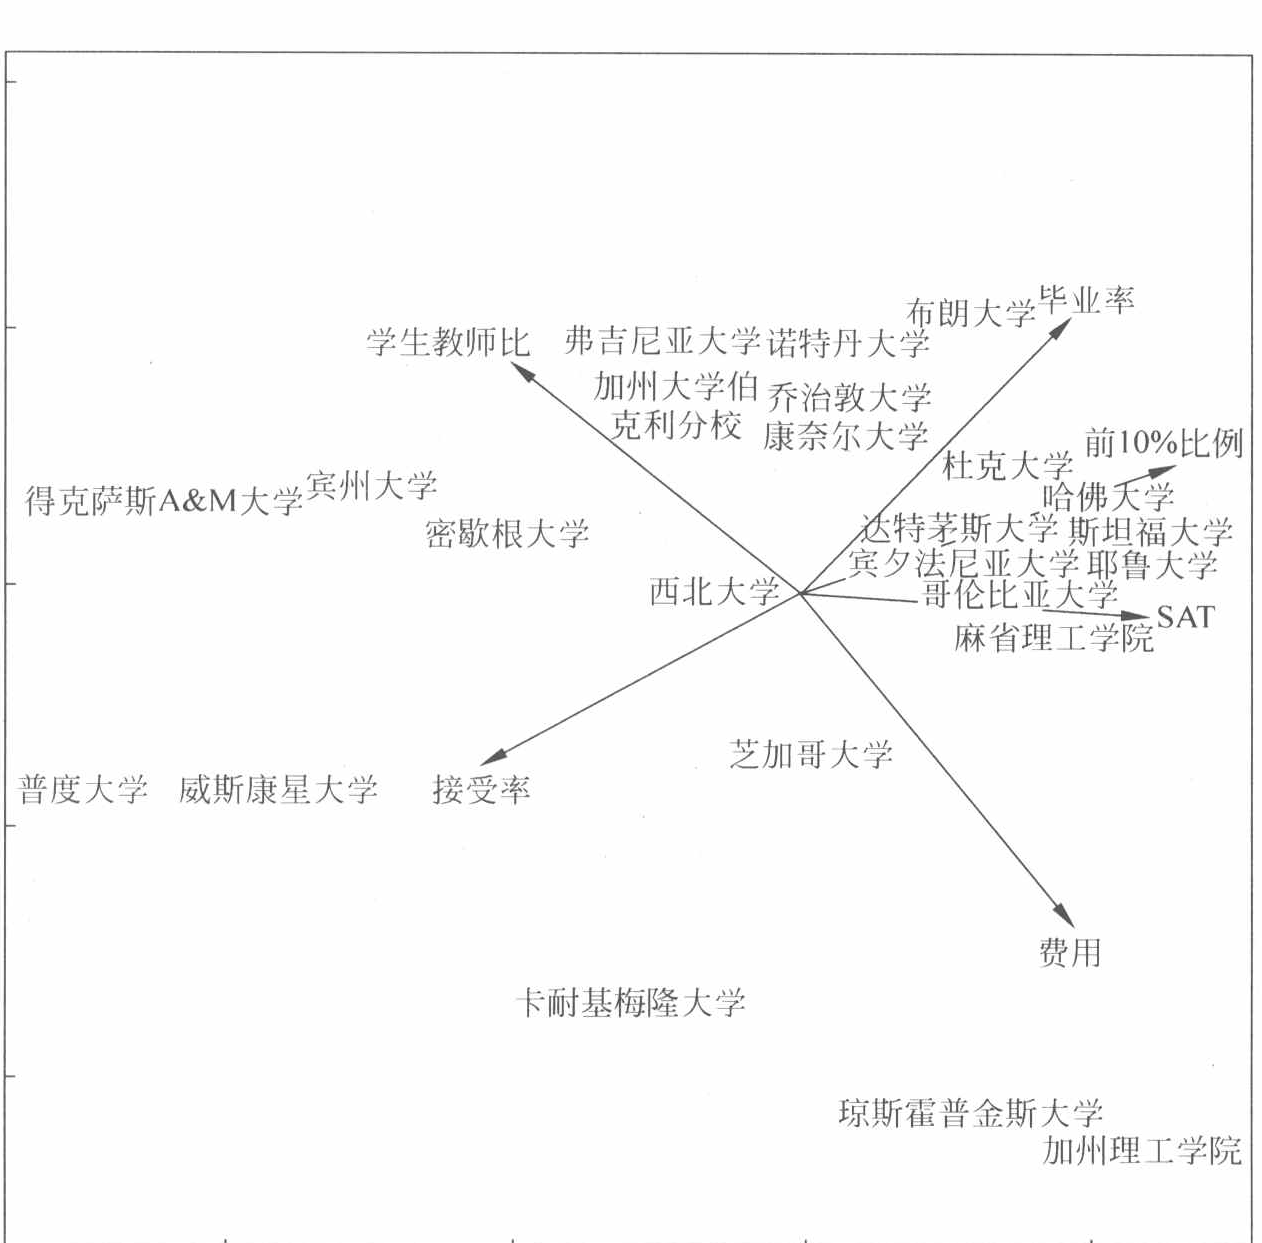
\includegraphics[width=106.8mm]{figs/fig_pg580_1.png}
\phantomsection\label{fig:12.24}\mvcap{图 12.24\quad 大学数据的双重信息图}
\end{mvfigure}

\noindent$\bullet$\quad 主成分的两个轴是隐藏的.

\noindent$\bullet$\quad 每个变量有一个轴, 并有尺度.

作为原始的双重信息图, 第 $i$ 个项目的位置由前两个主成分的对应值确定:
\[
(\hat{y}_{1i},\hat{y}_{2i})=\left((\mathbf{x}_i-\bar{\mathbf{x}})'\hat{\mathbf{e}}_1,
(\mathbf{x}_i-\bar{\mathbf{x}})'\hat{\mathbf{e}}_2\right)
\]
其中 $\hat{\mathbf{e}}_1$ 和 $\hat{\mathbf{e}}_2$ 为 $\mathbf{S}$ 的前两个特征向量. 主成分的尺度在图上没有表示.

此外, 原始的双重信息图中表示变量的箭头用两个方向的刻度轴代替. 如同在用箭头表示的情况时一样, 第 $i$ 个变量的轴由 $\hat{\mathbf{E}}=[\hat{\mathbf{e}}_1,\hat{\mathbf{e}}_2]$ 的第 $i$ 行确定.

为进一步解释, 我们首先令 $\mathbf{u}_i$ 代表第 $i$ 元素为 1, 其他元素为 0 的向量. 任一 $p\times 1$ 向量 $\mathbf{x}$ 可表示为
\[
\mathbf{x}=\sum_{i=1}^{p}x_i\mathbf{u}_i
\]
并且由定义 2A.12, $\mathbf{x}$ 到前两个特征向量生成的空间上的投影有系数向量
\[
\hat{\mathbf{E}}'\mathbf{x}=\sum_{i=1}^{p}x_i(\hat{\mathbf{E}}'\mathbf{u}_i)
\]
因此第 $i$ 个变量对上述向量和的贡献为 $x_i(\hat{\mathbf{E}}'\mathbf{u}_i)=x_i(e_{i1},e_{i2})'$. $\hat{\mathbf{E}}$ 的第 $i$ 行的元素 $e_{i1}$ 和 $e_{i2}$ 决定第 $i$ 个变量的轴的方向.

%% ===== pg-581 =====

% ---- pg-581 （书页 569） ----

样本均值 $\bar{\mathbf{x}}=\sum_{i=1}^{p}\bar{x}_i\mathbf{u}_i$ 的投影向量
\[
\hat{\mathbf{E}}'\bar{\mathbf{x}}=\sum_{i=1}^{p}\bar{x}_i(\hat{\mathbf{E}}'\mathbf{u}_i)
\]
是双向信息图的原点. 每个 $\mathbf{x}$ 可表示为 $\mathbf{x}=\bar{\mathbf{x}}+(\mathbf{x}-\bar{\mathbf{x}})$, 因此其投影向量有两个分量
\[
\sum_{i=1}^{p}\bar{x}_i(\hat{\mathbf{E}}'\mathbf{u}_i)+\sum_{i=1}^{p}(x_i-\bar{x}_i)(\hat{\mathbf{E}}'\mathbf{u}_i)
\]
从原点出发, 将点沿方向 $w(e_{1i},e_{2i})'$ 布置, $w=0,\pm1,\pm2,\cdots$. 这样就对均值中心化的变量 $x_i-\bar{x}_i$ 提供了尺度. 如此, $x_i$ 的单位变化定义了双重信息图中的距离. 但是第 $i$ 个变量的原点对应于 $w=0$, 因为 $\sum_{i=1}^{p}\bar{x}_i(\hat{\mathbf{E}}'\mathbf{u}_i)$ 项被忽略了. 轴的标度需要作平移使得双重信息图的原点为 $\bar{x}_i$. 由于 $\bar{x}_i$ 通常不是整数(或其他好的数), 可以选择与其最接近的整数(或其他好的数)来表示, 同时刻度也适当地平移. 计算机软件能将这个有一定困难的任务简化.

标注尺度使得我们可以将 $x_i(e_{1i},e_{2i})'$ 的位置可视地表示在双向信息图中. 标注尺度只是预测变量的值, 而不是变量的真实值, 因为所标注的尺度是基于二维逼近.

\noindent\textbf{例 12.20}\quad (大学数据的另一种双重信息图)

\begin{mvfigure}
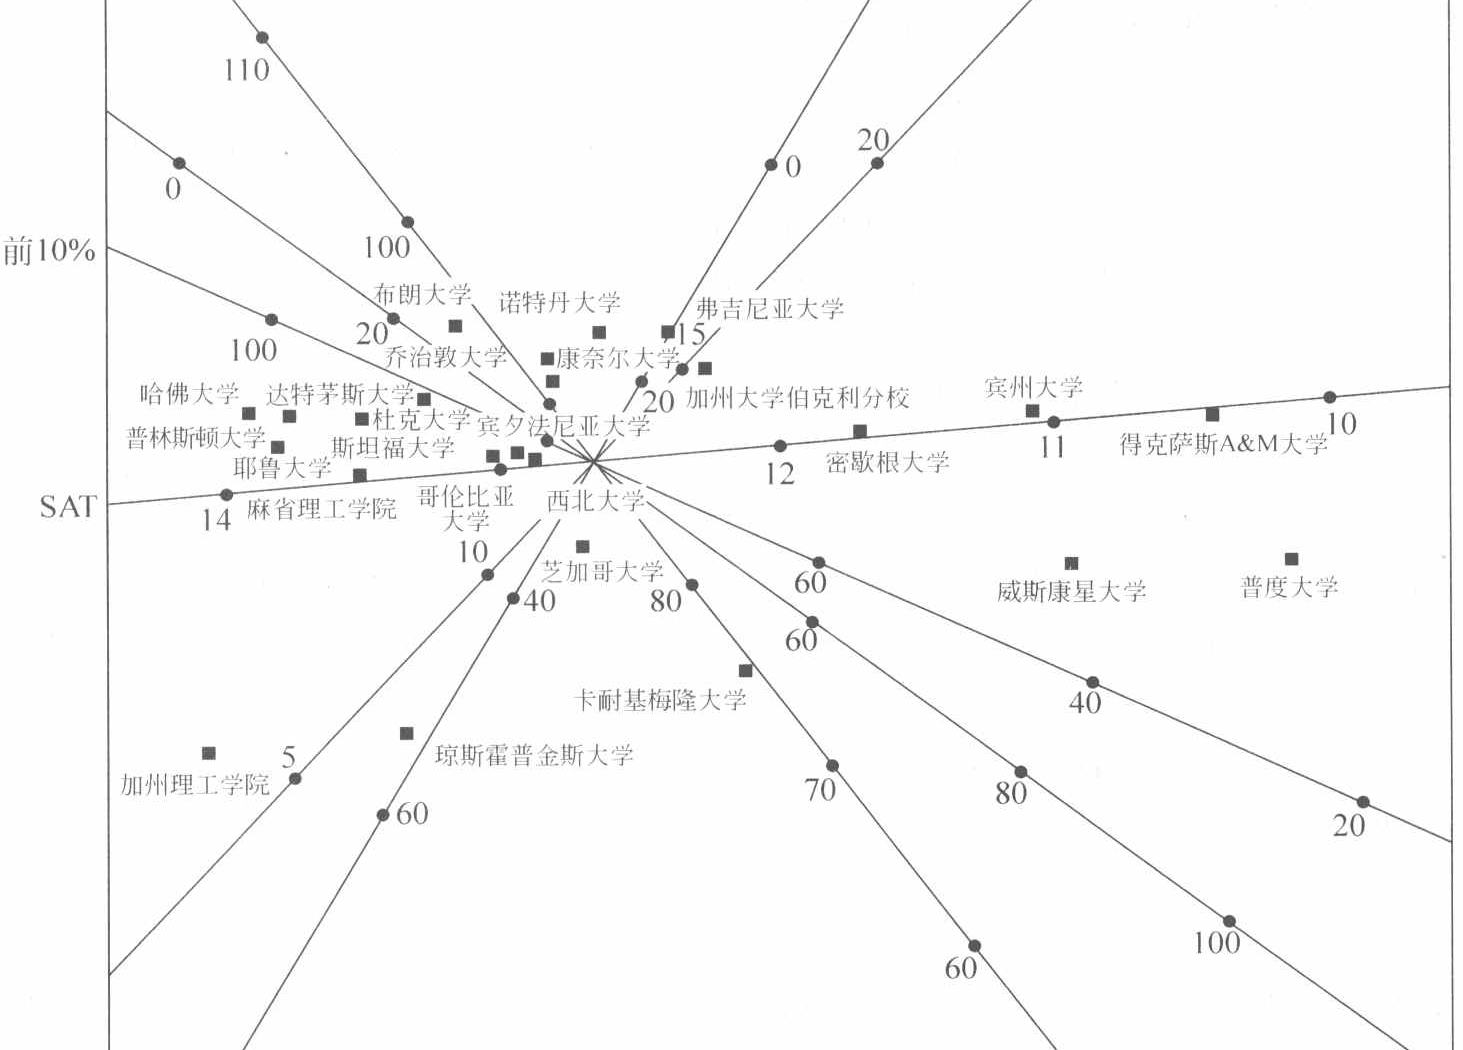
\includegraphics[width=123.8mm]{figs/fig_pg581_1.png}
\phantomsection\label{fig:12.25}\mvcap{图 12.25\quad 大学数据的另一种双重信息图}
\end{mvfigure}

%% ===== pg-582 =====

% ---- pg-582 （书页 570） ----

我们用\hyperref[tab:12.9]{表 12.9} 中的大学数据来说明这个新的双重信息图方法. 新的双重信息图显示在\hyperref[fig:12.25]{图 12.25} 中, 其中每个变量有一个轴. 与\hyperref[fig:12.24]{图 12.24} 比较, 计算机软件将第一主成分的轴调转了方向. 注意, 费用和学生教师比将加州理工学院和琼斯霍普金斯大学两所大学与其他大学分离开. 加州理工学院和琼斯霍普金斯大学两所大学费用为每年大致 5.7 万美元, 而学生教师比只有一位数字. 在图中右侧的大的州立大学有相对较高的学生教师比, 大约在 20 左右, 而入学新生的 SAT 得分相对较低, 并且在入学新生中, 只有 50\% 或更低比例的人在高中是前 10\% 的优等生. 新双重信息图中的尺度化轴比原来的双重信息图中的箭头可显示更多信息. \hfill$\blacksquare$

更多关于新双重信息图的案例和关于合适的专用统计软件的文献可以从文献[23]中查到.

\section{普罗克鲁斯特斯分析:一种比较点结构的方法}
\phantomsection\label{sec:12.9}

从一个与 $n$ 个对象有关的给定的 $n\times n$ 距离阵 $\mathbf{D}$ 或相似阵 $\mathbf{S}$ 出发, 用不同的方法可以得到两种或两种以上的点结构. 可能的方法包括度量和非度量的多维标度变换两种. 一个自然会提出的问题是: 两种方法的解在多大的程度上互相一致? 在例 12.16 中, \hyperref[fig:12.19]{图 12.19} 和 12.20 分别给出大学数据的度量多维标度变换（主坐标分析）和非度量多维标度变换的解. 这两个点结构看上去颇相似, 但给出一个定量的量会是有用的. 将两个结构之一适当移动, 使得它与另一个结构尽可能对齐, 从而得到这两个结构的一个数值比较, 这种方法称为普罗克鲁斯特斯分析. 这个方法的名称源于希腊神话中一个旅店老板普罗克鲁斯特斯的名字, 他对每一个到他店中投宿的旅客都要强行拉长或砍去他们的脚, 以便同他的床的长度相适应.

\mvsub{构造普罗克鲁斯特斯一致性度量}

设 $n\times p$ 矩阵 $\mathbf{X}^{*}$ 包含用方法 1 得到的 $n$ 个点的坐标, 而 $n\times q$ 矩阵 $\mathbf{Y}^{*}$ 包含用方法 2 得到的 $n$ 个点的坐标, 其中 $q\leqslant p$. 通过在 $\mathbf{Y}^{*}$ 中添加一些全部为 0 的列, 我们可以假定 $q=p$, 因此 $\mathbf{X}^{*}$ 和 $\mathbf{Y}^{*}$ 都是 $n\times p$ 阵. 为确定这两个结构能否相容, 我们可以比方说移动第二个结构, 使之与第一个结构相匹配. 做法是将第一个结构中的每一点平移, 并将该结构绕坐标轴转动或进行反射变换.\footnote{西布森(Sibson, 见文献[30])建议将下面的系数用作两个结构的一致性度量:
\[
\gamma=1-\frac{[\mathrm{tr}(\mathbf{Y}^{*\prime}\mathbf{X}^{*}\mathbf{X}^{*\prime}\mathbf{Y}^{*})^{1/2}]^{2}}{\mathrm{tr}(\mathbf{X}^{*\prime}\mathbf{X}^{*})\mathrm{tr}(\mathbf{Y}^{*\prime}\mathbf{Y}^{*})}
\]
对完全相同的结构, $\gamma=0$. 如有必要, 在完成普罗克鲁斯特斯分析后可将 $\gamma$ 算出.}

数学上说, 对第 $j$ 个点的坐标向量 $\mathbf{y}_{j}$ 加一个平移向量 $\mathbf{b}$ 并乘一个正交阵 $\mathbf{Q}$ 之后, 就将它变换成
\[
\mathbf{Q}\mathbf{y}_{j}+\mathbf{b}
\]
然后改变向量 $\mathbf{b}$ 和正交阵 $\mathbf{Q}$ 使得两个结构中全部 $n$ 对对应点之间的平方距离之和达到最小. 第一个结构中第 $j$ 个点的坐标 $\mathbf{x}_{j}$ 与第二个结构中变换后的对应点坐标 $\mathbf{Q}\mathbf{y}_{j}+\mathbf{b}$ 之间的平方距离为
\phantomsection\label{eq:12-48}
\begin{equation}
d_{j}^{2}(\mathbf{x}_{j},\mathbf{Q}\mathbf{y}_{j}+\mathbf{b})=(\mathbf{x}_{j}-\mathbf{Q}\mathbf{y}_{j}-\mathbf{b})'(\mathbf{x}_{j}-\mathbf{Q}\mathbf{y}_{j}-\mathbf{b}) \tag{12-48}
\end{equation}
我们将残差平方和
\phantomsection\label{eq:12-49}
\begin{equation}
PR^{2}=\min_{\mathbf{Q},\mathbf{b}}\sum_{j=1}^{n}(\mathbf{x}_{j}-\mathbf{Q}\mathbf{y}_{j}-\mathbf{b})'(\mathbf{x}_{j}-\mathbf{Q}\mathbf{y}_{j}-\mathbf{b}) \tag{12-49}
\end{equation}
取作两个结构间的拟合量度或一致性量度. 下面的结果告诉我们, 如何计算这个普罗克鲁斯

%% ===== pg-583 =====

% ---- pg-583 （书页 571） ----

特斯一致性残差平方和量度, 以及如何确定 $\mathbf{Y}^{*}$ 相对 $\mathbf{X}^{*}$ 的普罗克鲁斯特斯旋转.

\mvthm{结论 12.2}{设 $n\times p$ 结构 $\mathbf{X}^{*}$ 和 $\mathbf{Y}^{*}$ 均已中心化, 即各行均值皆为零, 此时}
\phantomsection\label{eq:12-50}
\begin{equation}
\begin{aligned}
PR^{2}&=\sum_{j=1}^{n}\mathbf{x}_{j}'\mathbf{x}_{j}+\sum_{j=1}^{n}\mathbf{y}_{j}'\mathbf{y}_{j}-2\sum_{i=1}^{p}\lambda_{i}\\
&=\mathrm{tr}[\mathbf{X}^{*}\mathbf{X}^{*\prime}]+\mathrm{tr}[\mathbf{Y}^{*}\mathbf{Y}^{*\prime}]-2\mathrm{tr}[\boldsymbol{\Lambda}]
\end{aligned}
\tag{12-50}
\end{equation}
其中 $\boldsymbol{\Lambda}=$ 对角$(\lambda_{1},\lambda_{2},\cdots,\lambda_{p})$, 最小化变换为
\phantomsection\label{eq:12-51}
\begin{equation}
\hat{\mathbf{Q}}=\sum_{i=1}^{p}\mathbf{v}_{i}\mathbf{u}_{i}'=\mathbf{V}\mathbf{U}'\qquad \hat{\mathbf{b}}=\mathbf{0} \tag{12-51}
\end{equation}
这里 $\boldsymbol{\Lambda},\mathbf{U}$ 和 $\mathbf{V}$ 由下面的奇异值分解得到:
\[
\sum_{j=1}^{n}\mathbf{y}_{j}\mathbf{x}_{j}'=\underset{(p\times n)}{\mathbf{Y}^{*\prime}}\underset{(n\times p)}{\mathbf{X}^{*}}=\underset{(p\times p)}{\mathbf{U}}\underset{(p\times p)}{\boldsymbol{\Lambda}}\underset{(p\times p)}{\mathbf{V}'}
\]

证明\quad 由于两个点结构是已实现零均值中心化$\left(\sum_{j=1}^{n}\mathbf{x}_{j}=\mathbf{0}, \text{及} \sum_{j=1}^{n}\mathbf{y}_{j}=\mathbf{0}\right)$, 我们有
\[
\sum_{j=1}^{n}(\mathbf{x}_{j}-\mathbf{Q}\mathbf{y}_{j}-\mathbf{b})'(\mathbf{x}_{j}-\mathbf{Q}\mathbf{y}_{j}-\mathbf{b})=\sum_{j=1}^{n}(\mathbf{x}_{j}-\mathbf{Q}\mathbf{y}_{j})'(\mathbf{x}_{j}-\mathbf{Q}\mathbf{y}_{j})+n\mathbf{b}'\mathbf{b}
\]
右端的最后一项为非负项, 因此当 $\hat{\mathbf{b}}=\mathbf{0}$ 有最佳拟合. 因此我们只需考虑
\[
PR^{2}=\min_{\mathbf{Q}}\sum_{j=1}^{n}(\mathbf{x}_{j}-\mathbf{Q}\mathbf{y}_{j})'(\mathbf{x}_{j}-\mathbf{Q}\mathbf{y}_{j})=\sum_{j=1}^{n}\mathbf{x}_{j}'\mathbf{x}_{j}+\sum_{j=1}^{n}\mathbf{y}_{j}'\mathbf{y}_{j}-2\max_{\mathbf{Q}}\sum_{j=1}^{n}\mathbf{x}_{j}'\mathbf{Q}\mathbf{y}_{j}
\]
利用 $\mathbf{x}_{j}'\mathbf{Q}\mathbf{y}_{j}=\mathrm{tr}[\mathbf{Q}\mathbf{y}_{j}\mathbf{x}_{j}']$, 可将上式右端最大化的表达式变成
\[
\sum_{j=1}^{n}\mathbf{x}_{j}'\mathbf{Q}\mathbf{y}_{j}=\sum_{j=1}^{n}\mathrm{tr}[\mathbf{Q}\mathbf{y}_{j}\mathbf{x}_{j}']=\mathrm{tr}\left[\mathbf{Q}\sum_{j=1}^{n}\mathbf{y}_{j}\mathbf{x}_{j}'\right]
\]
由奇异值分解,
\[
\sum_{j=1}^{n}\mathbf{y}_{j}\mathbf{x}_{j}'=\mathbf{Y}^{*\prime}\mathbf{X}^{*}=\mathbf{U}\boldsymbol{\Lambda}\mathbf{V}'=\sum_{i=1}^{p}\lambda_{i}\mathbf{u}_{i}\mathbf{v}_{i}'
\]
其中 $\mathbf{U}=[\mathbf{u}_{1},\mathbf{u}_{2},\cdots,\mathbf{u}_{p}],\mathbf{V}=[\mathbf{v}_{1},\mathbf{v}_{2},\cdots,\mathbf{v}_{p}]$ 为 $p\times p$ 正交矩阵. 因此,
\[
\sum_{j=1}^{n}\mathbf{x}_{j}'\mathbf{Q}\mathbf{y}_{j}=\mathrm{tr}\left[\mathbf{Q}\left(\sum_{i=1}^{p}\lambda_{i}\mathbf{u}_{i}\mathbf{v}_{i}'\right)\right]=\sum_{i=1}^{p}\lambda_{i}\mathrm{tr}[\mathbf{Q}\mathbf{u}_{i}\mathbf{v}_{i}']
\]
上式右端第 $i$ 项中可变的量
\[
\mathrm{tr}[\mathbf{Q}\mathbf{u}_{i}\mathbf{v}_{i}']=\mathbf{v}_{i}'\mathbf{Q}\mathbf{u}_{i}
\]
有上界 1. 这可以用柯西-施瓦茨不等式[见\hyperref[eq:2-48]{式(2-48)}]并令 $\mathbf{b}=\mathbf{Q}\mathbf{v}_{i}$ 和 $\mathbf{d}=\mathbf{u}_{i}$ 来证明. 也就是说
\[
\mathbf{v}_{i}'\mathbf{Q}\mathbf{u}_{i}\leqslant\sqrt{\mathbf{v}_{i}'\mathbf{Q}'\mathbf{Q}\mathbf{v}_{i}}\sqrt{\mathbf{u}_{i}'\mathbf{u}_{i}}=\sqrt{\mathbf{v}_{i}'\mathbf{v}_{i}}\times 1=1
\]
所有 $p$ 个这样的项, 都可以令 $\hat{\mathbf{Q}}=\mathbf{V}\mathbf{U}'$ 使之达到最大. 在这种选择下,
\[
\mathbf{v}_{i}'\hat{\mathbf{Q}}\mathbf{u}_{i}=\mathbf{v}_{i}'\mathbf{V}\mathbf{U}'\mathbf{u}_{i}
=[0,\cdots,0,1,0,\cdots,0]
\begin{bmatrix}
0\\ \vdots\\ 0\\ 1\\ 0\\ \vdots\\ 0
\end{bmatrix}=1
\]
因此

%% ===== pg-584 =====

% ---- pg-584 （书页 572） ----

\[
-2\max_{\mathbf{Q}}\sum_{j=1}^{n}\mathbf{x}_{j}'\mathbf{Q}\mathbf{y}_{j}=-2(\lambda_{1}+\lambda_{2}+\cdots+\lambda_{p})
\]
最后, 我们证实 $\mathbf{Q}\mathbf{Q}'=\mathbf{V}\mathbf{U}'\mathbf{U}\mathbf{V}'=\mathbf{V}\mathbf{I}_{p}\mathbf{V}'=\mathbf{I}_{p}$, 因此 $\mathbf{Q}$ 是 $p\times p$ 正交阵.

\noindent\textbf{例 12.21}\quad (大学数据的普罗克鲁斯特斯分析)

用度量和非度量多维标度变换对例 12.16 中所给的大学数据进行分析后得出两个点结构. 这两个点结构看上去很接近. 对两种标度变换方法各有一个二维坐标系. 最初, 平方距离之和为
\[
\sum_{j=1}^{25}(\mathbf{x}_{j}-\mathbf{y}_{j})'(\mathbf{x}_{j}-\mathbf{y}_{j})=3.862
\]
计算机计算给出
\[
\mathbf{U}=\begin{bmatrix}-0.999\,0&0.044\,8\\0.044\,8&0.999\,0\end{bmatrix},\qquad
\mathbf{V}=\begin{bmatrix}-1.000\,0&0.007\,6\\0.007\,6&1.000\,0\end{bmatrix},\qquad
\boldsymbol{\Lambda}=\begin{bmatrix}114.943\,9&0.000\\0.000&21.367\,3\end{bmatrix}
\]
根据结论 12.2, 为最好地“对齐”这两个解, 我们对非度量标度变换解乘以正交矩阵
\[
\hat{\mathbf{Q}}=\sum_{i=1}^{2}\mathbf{v}_{i}\mathbf{u}_{i}'=\mathbf{V}\mathbf{U}'=\begin{bmatrix}0.999\,3&-0.037\,2\\0.037\,2&0.999\,3\end{bmatrix}
\]
这个变换大致相当于将非度量解沿顺时针方向旋转大约 2 度. 经过旋转后, 平方距离之和由 3.862 减少到普罗克鲁斯特斯拟合量度
\[
PR^{2}=\sum_{j=1}^{25}\mathbf{x}_{j}'\mathbf{x}_{j}+\sum_{j=1}^{25}\mathbf{y}_{j}'\mathbf{y}_{j}-2\sum_{i=1}^{2}\lambda_{i}=3.673
\]
\hfill$\blacksquare$

\noindent\textbf{例 12.22}\quad (森林数据的普罗克鲁斯特斯分析及附加定位)

在威斯康星州南部的 10 处高地收集了 8 种树的数据. 这些数据列于\hyperref[tab:12.10]{表 12.10} 中.

\begin{mvtable}
\phantomsection\label{tab:12.10}\mvtabcap{表 12.10\quad 威斯康星森林数据}
\begin{tabular}{l|cccccccccc}
\toprule
树种 & \multicolumn{10}{c}{场\quad 所}\\
\cmidrule(lr){2-11}
 & 1 & 2 & 3 & 4 & 5 & 6 & 7 & 8 & 9 & 10\\
\midrule
针橡 & 9 & 8 & 3 & 5 & 6 & 0 & 5 & 0 & 0 & 0\\
黑橡 & 8 & 9 & 8 & 7 & 0 & 0 & 0 & 0 & 0 & 0\\
白橡 & 5 & 4 & 9 & 9 & 7 & 7 & 4 & 6 & 0 & 2\\
红橡 & 3 & 4 & 0 & 6 & 9 & 8 & 7 & 6 & 4 & 3\\
美国榆 & 2 & 2 & 4 & 5 & 6 & 0 & 5 & 0 & 2 & 5\\
菩提 & 0 & 0 & 0 & 0 & 2 & 7 & 6 & 6 & 7 & 6\\
铁树 & 0 & 0 & 0 & 0 & 0 & 0 & 7 & 4 & 6 & 5\\
糖枫 & 0 & 0 & 0 & 0 & 0 & 5 & 4 & 8 & 8 & 9\\
\bottomrule
\end{tabular}

资料来源: 见文献[24].
\end{mvtable}

度量多维标度变换法（或主坐标法）和非度量标度变换法的解分别示于\hyperref[fig:12.26]{图 12.26} 和图 12.27.

利用\hyperref[fig:12.26]{图 12.26} 和图 12.27 中各点的坐标, 我们得到两个点结构的初始平方距离和为
\[
\sum_{j=1}^{10}(\mathbf{x}_{j}-\mathbf{y}_{j})'(\mathbf{x}_{j}-\mathbf{y}_{j})=8.547
\]
计算机计算给出
\[
\mathbf{U}=\begin{bmatrix}-0.983\,3&-0.182\,1\\-0.182\,1&0.983\,3\end{bmatrix},\qquad
\mathbf{V}=\begin{bmatrix}-1.000\,0&-0.000\,1\\-0.000\,1&1.000\,0\end{bmatrix},
\]

%% ===== pg-585 =====

% ---- pg-585 （书页 573） ----

\begin{mvfigure}
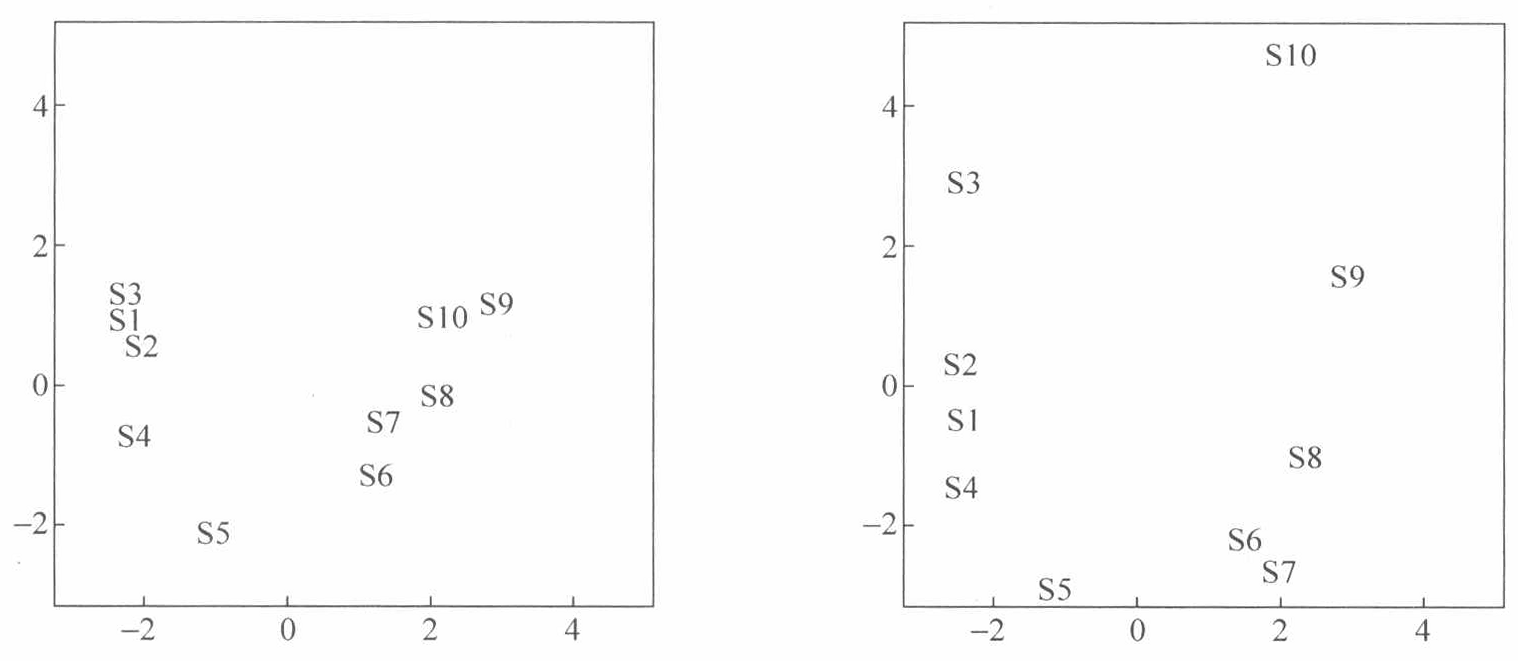
\includegraphics[width=128.5mm]{figs/fig_pg585_1.png}
\phantomsection\label{fig:12.26}\mvcap{图 12.26\quad 森林数据的度量多维标度变换 \qquad 图 12.27\quad 森林数据的非度量多维标度变换}
\end{mvfigure}

\[
\boldsymbol{\Lambda}=\begin{bmatrix}43.374\,8&0.000\\0.000&14.910\,3\end{bmatrix}
\]
根据结论 12.2, 为更好地对齐两个解, 我们对非度量标度变换解乘以正交矩阵
\[
\hat{\mathbf{Q}}=\sum_{i=1}^{2}\mathbf{v}_{i}\mathbf{u}_{i}'=\mathbf{V}\mathbf{U}'=\begin{bmatrix}0.983\,3&0.182\,1\\-0.182\,1&0.983\,3\end{bmatrix}
\]
这相当于将非度量解沿顺时针方向旋转大约 10 度. 旋转后, 平方距离从 8.547 减少到普罗克鲁斯特斯拟合量度
\[
PR^{2}=\sum_{j=1}^{10}\mathbf{x}_{j}'\mathbf{x}_{j}+\sum_{j=1}^{10}\mathbf{y}_{j}'\mathbf{y}_{j}-2\sum_{i=1}^{2}\lambda_{i}=6.599
\]
我们注意到抽样场所在两个图中都大致位于一条曲线附近. 这就有可能对数据作一维的非线性排序. 可以用二次或其他曲线来拟合这些点. 通过对曲线施加一个标度, 我们可以得到一个一维排序.

如果将威斯康星森林数据中的抽样单元和变量同时显示在图中, 就会有更多信息. 对数据进行对应分析得到\hyperref[fig:12.28]{图 12.28} 的点图. 同一组数据的双重信息图示于\hyperref[fig:12.29]{图 12.29}.

\begin{mvfigure}
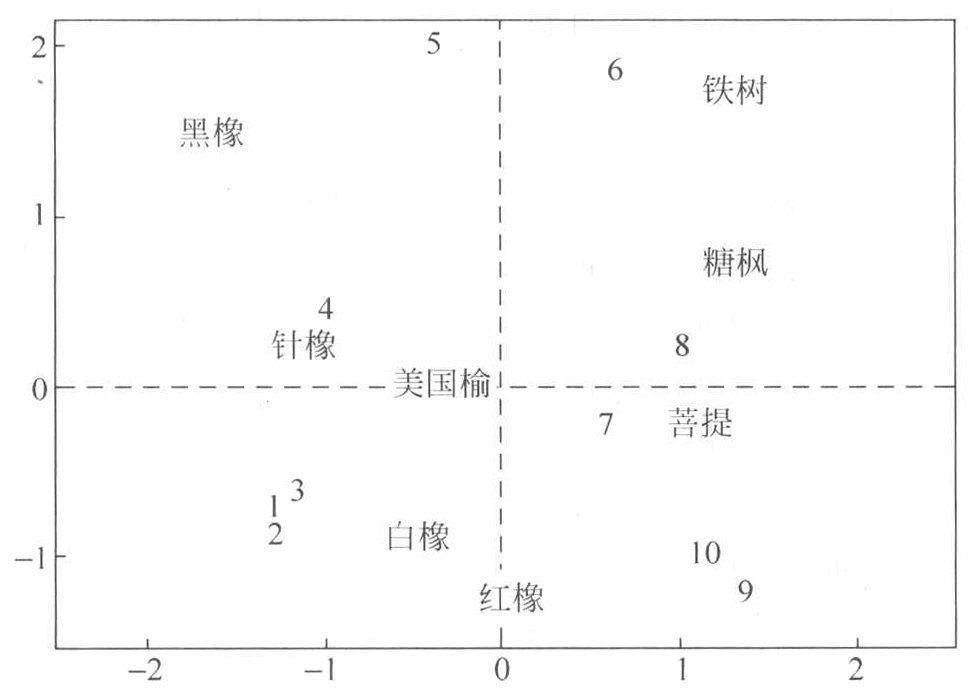
\includegraphics[width=82.0mm]{figs/fig_pg585_2.png}
\phantomsection\label{fig:12.28}\mvcap{图 12.28\quad 森林数据的对应分析图}
\end{mvfigure}

%% ===== pg-586 =====

% ---- pg-586 （书页 574） ----

\begin{mvfigure}
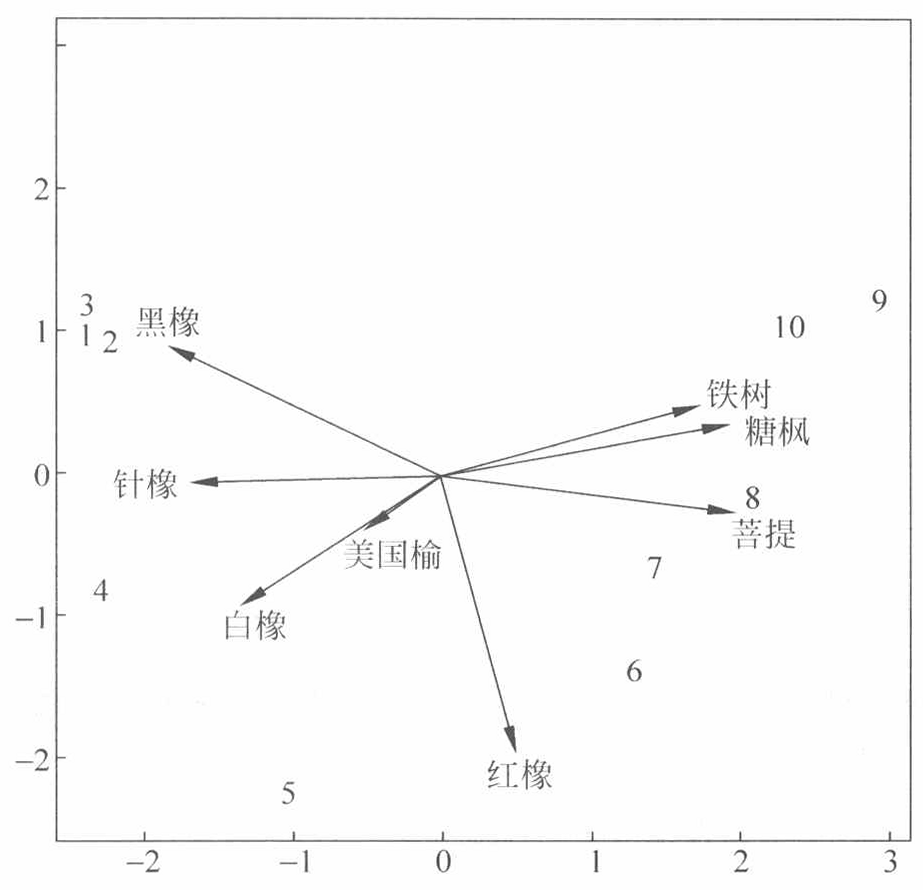
\includegraphics[width=78.1mm]{figs/fig_pg586_1.png}
\phantomsection\label{fig:12.29}\mvcap{图 12.29\quad 森林数据的双重信息图}
\end{mvfigure}

这两个点图给出非常相似的信息. 场所 1 至 5 倾向于与橡树类相联系, 而场所 7 至 10 倾向于与菩提树、铁树和糖枫相联系. 美国榆树分布在大部分场所. 由不同树种区分的场所几乎是连续的. \hfill$\blacksquare$

\mvsub{补充 12A\quad 数据挖掘}

\mvsub{引言}

在传统的统计方法中, 关于大约 50 个变量的 10 000 个观测意味着一组非常大的样本. 而今天, 基于计算机的数据存储设备可以存储万亿字节的数据. 对于某些组织, 处理的数据在最近几十年里增长了上十万倍. 电信、银行、制药以及集装箱航运等行业中都有一些公司有巨大的数据库. 考虑下面的例子. 假定在议会图书馆中的 1 700 万本图书平均相当于 MS Word 格式中大小为 1MB 的文本, 则将这些印刷材料输入计算机数据库将占用 17 万亿字节的磁盘空间. 联合邮递服务公司(United Parcel Service, UPS)有一个 17 万亿字节的数据库来管理其业务.

就我们的目标来说, 数据挖掘(data mining)意味着在极其巨大的数据内发现模式或者关系. 也就是说, 数据挖掘是要从数值信息的大山中挖掘出少量知识的金块. 从商业角度说, 这些知识的金块代表“活的”信息, 有助于发现获得竞争优势的方法.

数据挖掘需要用适合的软件和快速的计算机. 显而易见, 本书中介绍的各种数据分析技术与机器学习以及人工智能中开发的各种算法在数据挖掘中扮演着重要角色. 开发著名的统计软件包的公司现在提供包罗万象的数据挖掘程序.\footnote{SAS 公司的数据挖掘程序现在称为 Enterprise Miner. SPSS 的数据挖掘程序是 Clementine.} 此外, 一些特殊用途的程序, 如 CART, 在数据挖掘的应用中已经取得成功.

数据挖掘帮助确定用于处方药物的化学成分, 发现欺诈索赔和购买, 创建并维护个人客

%% ===== pg-587 =====

% ---- pg-587 （书页 575） ----

户的联系, 设计更好的引擎并建立适当的设备, 创建更好的医疗程序, 改进过程控制, 并且发展有效的信用评分法则.

在传统的统计应用中, 样本容量相对较小, 数据是小心地搜集到的, 样本分析结果为统计推断提供了基础, 虽然也处理异常情况但不是首要关注, 通常高度依赖模型. 在数据挖掘中, 样本容量巨大, 数据是分散的, 有历史关系的(日复一日地记录), 样本用于训练、验证和检验(非正式的推断), 关注异常情况, 通常不建立模型. 不仅如此, 数据的准备(包括数据的搜集、评估和整理, 变量的定义和选择)通常是费力的任务, 大约在数据挖掘的工作中占 60\%$\sim$80\% 的比例.

数据挖掘的问题大致可分为以下几个内容:

\noindent$\bullet$\quad 分类(离散结果):

\noindent\hspace*{1.5em}谁可能改用另一家移动通信服务公司?

\noindent$\bullet$\quad 预测(连续结果):

\noindent\hspace*{1.5em}这栋房子的适当估价是多少?

\noindent$\bullet$\quad 关联/市场篮子分析:

\noindent\hspace*{1.5em}脱脂奶是否经常与低脂奶酪一起被购买?

\noindent$\bullet$\quad 聚类:

\noindent\hspace*{1.5em}是否存在有相同购买习惯的顾客?

\noindent$\bullet$\quad 描述:

\noindent\hspace*{1.5em}星期四, 杂货店的顾客通常同时购买玉米片和软饮料.

鉴于数据挖掘问题的特性, 不难理解为什么本书中讨论的许多统计方法构成完备的数据挖掘软件的重要部分. 具体地说, 回归、判别和分类程序(线性法则、逻辑斯蒂回归、决策树等)以及聚类算法是非常重要的数据挖掘工具. 其他工具包括关联法则, 多重适应回归样条(MARS), $K$ 近邻算法, 神经网络, 遗传算法以及可视化等. 这些方法超出了本书的范围.\textsuperscript{①}

\mvsub{数据挖掘的过程}

数据挖掘的过程有一系列步骤. 这些步骤构成一种策略, 与任何其他的建模过程的策略没有本质的不同. 具体而言, 数据挖掘必须

\noindent 1.\quad 廓清问题, 确定目标.

\noindent 2.\quad 收集和准备合适的数据.

\noindent 3.\quad 从数据中发现可能的关联、未察觉的特性以及显而易见的异常情况, 以得到深入的认识.

\noindent 4.\quad 清理数据并对变量作适当变换.

\noindent 5.\quad 将数据划分为训练、验证和检验数据集.

\noindent 6.\quad 对训练数据建立模型.

\noindent 7.\quad 用验证数据评估模型的好坏, 必要时修正模型.

\noindent 8.\quad 基于验证数据或检验数据评估模型的表现. 将模型输出与原始对象作比较. 考察模型是否有用.

\noindent 9.\quad 应用模型.

\vspace{6pt}
\noindent\rule{\linewidth}{0.4pt}
\par\vspace{2pt}
{\zihao{6}\noindent ①\quad 要得到更多的关于数据挖掘的一般信息和数据挖掘工具, 见本章末尾的参考文献.\par}

%% ===== pg-588 =====

% ---- pg-588 （书页 576） ----

10. 监控模型的运行. 考察结果是否可靠, 成本是否合算?

在实践中, 经常有必要重复某些步骤若干次, 直至得到满意的结果为止. 数据挖掘软件套件, 如 Enterprise Miner 和 Clementine 等, 通常按照上述的步骤序列设计, 并且可以在屏幕上以流程图的方式图示结果.

数据挖掘需要丰富的工具和算法. 分析者不仅要能熟练使用这些工具和算法, 而且还要对研究课题的内涵有扎实的知识(或者与对研究课题的内涵有扎实知识的人合作), 如此才能得到可接受的结果. 任何数据挖掘结果一旦得到便成为一个不断进行的动态过程. 要采集新数据并对之加工, 模型要更新或开发新模型, 并且根据新的经验加以调整. 糟糕的数据挖掘工作的成本很高, 因此必须进行谨慎的模型建构和评估.

\mvsub{模型评估}

在数据挖掘的建模阶段, 可能同时检验若干模型. 在下面的案例中, 我们简要讨论对一组公开的数据——德国信用数据——用各种方法解决信用评分问题(确定信用风险大小)的结果. 这些方法是: 逻辑斯蒂回归, 决策树方法, 以及神经网络. 固然数据挖掘者能控制制约单个模型开发的模型输入和某些参数, 但是在大多数数据挖掘的努力中很少有正式的统计推断. 模型的评估与比较通常是由相关领域的专家来作, 使用的工具基本是描述性的, 例如混淆矩阵、综合效益或损失数量、提升图、阈值控制图以及其他方法, 其中大部分是图方法.

将巨大的原始数据集划分为训练集、验证集和检验集, 就可以在评估潜在模型时使用没有用于建模的数据. 这样, 训练数据集用于建模. 模型用验证(提留)数据集评估. 如果在验证阶段模型表现不够满意, 则暂时保留. 在训练和验证两个阶段反复几次直到得到满意的模型为止. 此时, 经过训练和验证的模型要用检验数据来评估. 检验数据通常用于建模过程的末尾, 以保证对模型的性能有无偏的评估. 有时检验数据步被省略, 此时最终的评估基于验证样本或基于交叉验证.

一种重要的评估估计是\mvbold{提升图}(lift chart). 提升图可以有不同的构造方法, 但是都指示所选择的程序(模型)相对于基准活动的改进. 基准活动通常表示某种先验的信念或者随机指定. 提升图对比较不同的模型特别有用.

提升(lift)定义为
\[
\mathrm{Lift}=P(\text{结果}\,|\,\text{条件})/P(\text{结果})
\]
若结果独立于条件, 则 Lift$=1$. 当 Lift$>1$, 则说明条件(通常是模型或算法)会使结果发生的概率增大. 因此条件是有用的并有潜在的效益. 不同的条件可以用各自的提升图来比较.

\noindent\textbf{例 12.23}\quad (小的数据挖掘练习)

一组可以公开得到的数据集称为德国信用数据.\textsuperscript{①}这组数据有 $1\,000$ 个信用申请人的 20 个变量的数据, 并且记录了每个申请人最终的信用等级(“好”或“坏”). (数据挖掘的)目标是开发一种信用评分法则用于决定任一新的申请人的信用风险是低还是高, 依据是 20 个解释变量的值. 20 个解释变量包括 CHECKING(支票账号状况), DURATION(以月为单位的信用期限), HISTORY(信用历史), AMOUNT(信用额), AGE(年龄), OTHERS(其他分期付款债务), INSTALLP(分期付款占储蓄收入的百分比), 等等. 本质上, 我们要开发一个关于若干个

\vspace{6pt}
\noindent\rule{\linewidth}{0.4pt}
\par\vspace{2pt}
{\zihao{6}\noindent ①\quad 在写作本补充材料时, 德国信用数据可从 SAS 的 Enterprise Miner 软件伴随的样本数据文件中得到. 许多公开的数据集可从网页 www.kdnuggets.com 上下载.\par}

%% ===== pg-589 =====

% ---- pg-589 （书页 577） ----

变量的函数, 使得我们可以将任一新的申请人归入两个范畴: 低或高.

我们将使用在 11.7 节和 11.8 节中讨论的三种方法来开发分类程序. 这三种方法是: 逻辑斯蒂回归、分类树和神经网络. 对此三种方法的一个简要评估使我们可以比较这三种方法用于验证数据时的性能. 我们按照前面描述的一般数据挖掘程序, 用 SAS Enterprise Miner 软件完成此数据挖掘练习.

在整个信用数据集中, 70\% 的申请人为信用风险低, 30\% 为信用风险高. 原始数据分为两个子集: 训练集和验证集. 大约 60\% 的数据(581 个案例)归入训练集, 40\% 左右的数据归入验证集(419 个案例). 在分组时用随机抽样方法以保证在训练集和验证集中都大致有 70\% 低风险申请人和 30\% 高风险申请人. 下表是申请人信用分析的刻画.

\begin{mvtable}
\setlength{\tabcolsep}{16pt}%
\begin{tabular}{lccc}
\toprule
& \textbf{信用数据} & \textbf{训练数据} & \textbf{验证数据} \\
\midrule
好的 & 700 & 401 & 299 \\
坏的 & 300 & 180 & 120 \\
\cmidrule{2-4}
总数 & 1000 & 581 & 419 \\
\bottomrule
\end{tabular}
\end{mvtable}

\hyperref[fig:12.30]{图 12.30} 显示 Enterprise Miner 软件屏幕上的流程图. 图中的图标表示在数据挖掘过程中的行动. 例如, SAMPS10. DMAGESCR 包含数据; Data Partition 允许将数据划分为训练集、验证集和检验集; Transform Variables 允许对变量作变换; Regression, Tree 和 Neutral Network 三个图标可分别打开以开发各自的模型; Assessment 允许对每个模型作评估, 使用的方法有预测功效、提升、收益或损失等, 并可以对所有模型作比较.

\begin{mvfigure}
\begin{tikzpicture}[font=\zihao{6},every node/.style={inner sep=1pt}]
\tikzset{blk/.style={draw,minimum width=0.9cm,minimum height=0.7cm}}
% ---- 数据表图标 ----
\node[blk] (A) at (-6.0,0.0) {\tikz{\draw (0,0) rectangle (0.55,0.42);
  \foreach \y in {0.14,0.28} \draw (0,\y)--(0.55,\y);
  \foreach \x in {0.14,0.28,0.42} \draw (\x,0)--(\x,0.42);}};
\node[blk] (B) at (-4.2,0.35) {\tikz{\foreach \x in {0,0.14,0.28,0.42}
  \draw (\x,0.02) rectangle (\x+0.11,0.4); \draw (0,0.21)--(0.53,0.21);}};
\node[blk] (C) at (-2.4,0.0) {\tikz{\node at (0.28,0.21) {$f(x)$};}};
\node[blk] (D) at (-0.8,2.35) {\tikz{\draw (0,0)--(0,0.42)--(0.55,0.42);
  \draw (0.08,0.06)--(0.5,0.34);
  \fill (0.16,0.12) circle (0.022); \fill (0.32,0.22) circle (0.022); \fill (0.46,0.31) circle (0.022);}};
\node[blk] (E) at (-0.8,0.0) {\tikz{\fill (0.28,0.36) circle (0.03);
  \fill (0.08,0.06) circle (0.03); \fill (0.28,0.06) circle (0.03); \fill (0.48,0.06) circle (0.03);
  \draw (0.28,0.36)--(0.08,0.06); \draw (0.28,0.36)--(0.28,0.06); \draw (0.28,0.36)--(0.48,0.06);}};
\node[blk] (F) at (-0.8,-1.95) {\tikz{\foreach \y in {0.06,0.21,0.36} \fill (0.06,\y) circle (0.03);
  \fill (0.46,0.21) circle (0.03);
  \foreach \y in {0.06,0.21,0.36} \draw (0.06,\y)--(0.46,0.21);}};
\node[blk] (G) at (1.5,0.0) {\tikz{\draw (0.05,0.05) rectangle (0.42,0.4);
  \foreach \y in {0.14,0.24,0.34} \draw (0.1,\y)--(0.37,\y);
  \draw (0.38,0.3) circle (0.09); \draw (0.45,0.23)--(0.53,0.15);}};
\node[blk] (H) at (3.7,-0.1) {\tikz{\node at (0.28,0.21) {\$};}};
\node[blk] (I) at (5.9,-0.1) {\tikz{\draw (0.05,0.05) rectangle (0.18,0.2);
  \draw (0.2,0.05) rectangle (0.33,0.35); \draw (0.35,0.05) rectangle (0.48,0.28);
  \draw (0.02,0.05)--(0.51,0.05);}};
\node[blk] (J) at (3.7,-2.0) {\tikz{\draw (0,0) rectangle (0.55,0.42);
  \foreach \y in {0.14,0.28} \draw (0,\y)--(0.55,\y);
  \foreach \x in {0.14,0.28,0.42} \draw (\x,0)--(\x,0.42);}};
% ---- 标签 ----
\node[below=1pt,align=center] at (A.south) {SAMPS10.\\DMAGESCR};
\node[below=1pt,align=center] at (B.south) {Data\\Partition};
\node[below=1pt,align=center] at (C.south) {Transform\\Variables};
\node[below=1pt,align=center] at (D.south) {Regression};
\node[below=1pt,align=center] at (E.south) {Tree};
\node[below=1pt,align=center] at (F.south) {Neural\\Network};
\node[below=1pt,align=center] at (G.south) {Assessment};
\node[below=1pt,align=center] at (H.south) {Score!\\{}[Apply]};
\node[below=1pt,align=center] at (I.south) {Distribution\\Explorer};
\node[below=1pt,align=center] at (J.south) {SAMPS10.\\DMAGESCR};
% ---- 箭头 ----
\draw[-{Stealth}] (A.east) -- (B.west);
\draw[-{Stealth}] (B.east) -- (C.west);
\draw[-{Stealth}] (C.north east) -- (D.south west);
\draw[-{Stealth}] (C.east) -- (E.west);
\draw[-{Stealth}] (C.south east) -- (F.north west);
\draw[-{Stealth}] (D.south east) -- (G.north west);
\draw[-{Stealth}] (E.east) -- (G.west);
\draw[-{Stealth}] (F.north east) -- (G.south west);
\draw[-{Stealth}] (G.east) -- (H.west);
\draw[-{Stealth}] (H.east) -- (I.west);
\draw[-{Stealth}] (J.north) -- (H.south);
\end{tikzpicture}
\phantomsection\label{fig:12.30}\mvcap{图 12.30\quad 流程图}
\end{mvfigure}

最佳模型(及训练数据参数)可用于对新的申请人评分, 无须信用指派(SAMPS10. DMAGESCR). 在 Distribution Explorer 中, 得分结果可用各种方式表示.

对于本案例, 先验概率设置为数据比例, 即 $P(\text{低})=0.7,P(\text{高})=0.3$. 成本矩阵起初规定如下:

\begin{mvtable}
\setlength{\tabcolsep}{14pt}%
\begin{tabular}{cc|cc}
\toprule
\multicolumn{2}{c|}{} & \multicolumn{2}{c}{预测(决策)} \\
\cmidrule(lr){3-4}
\multicolumn{2}{c|}{} & 低(接受) & 高(拒绝) \\
\midrule
\multirow{2}{*}{实际} & 低 & 0 & 1 美元 \\
& 高 & 5 美元 & 0 \\
\bottomrule
\end{tabular}
\end{mvtable}

%% ===== pg-590 =====

% ---- pg-590 （书页 578） ----

因此, 将高风险申请人划分为“低”(接受)的代价是将低风险申请人划分为“高”(拒绝)的代价的 5 倍. 在实践中, 接受一个低的信用风险应该产生收益, 或负成本. 为满足此条件, 我们从成本矩阵的第一行减去 1 美元, 以获得更符合“实际”的成本矩阵如下:

\begin{mvtable}
\setlength{\tabcolsep}{14pt}%
\begin{tabular}{cc|cc}
\toprule
\multicolumn{2}{c|}{} & \multicolumn{2}{c}{预测(决策)} \\
\cmidrule(lr){3-4}
\multicolumn{2}{c|}{} & 低(接受) & 高(拒绝) \\
\midrule
\multirow{2}{*}{实际} & 低 & $-1$ 美元 & 0 \\
& 高 & 5 美元 & 0 \\
\bottomrule
\end{tabular}
\end{mvtable}

该成本矩阵与原来的矩阵产生相同的决策, 但是其结果从期望成本目标函数的角度更容易解释. 例如, 经过进一步的调整, 负的期望成本得分可能意味着潜在的收益, 因此申请人可能是低信用风险.

然后, 应该加工(变换)输入变量, 指定模型(或算法), 对流程图中每个图标设置需要的参数. 此时通过点击流程图中的任一图标可以执行程序到该点. 例如, 点击 Score 图标可以使程序从头执行到该图标(含). 在每个被执行的图标中的结果可以通过点击该图标得到.

我们用提升图解释模型评估. 这些提升图可从 Assessment 图标中得到.

考虑逻辑斯蒂回归分类. 逻辑斯蒂回归函数由训练数据确定, 用此函数对验证集的每个案例计算期望成本. 这些期望成本“得分”可以从小到大重新排序, 并且按照 10,20,$\cdots$ 百分位数分组. 第一个百分位组有 42(419 的 10\%)个申请人, 他们有最小的负期望成本(最大的潜在收益); 第二个百分位组同样有 42(419 的 10\%)个申请人, 如此类推. (从分类的观点看, 那些有负期望成本的申请人应被分入低风险, 而有正期望成本的申请人应被分入高风险.)

如果模型没有预测能力, 我们可以期望低信用风险在各个组内大致是均匀分布的. 也就是说, 在每个百分位组内的 42 个人中, 大致有 10\% 或 $0.10\times299=30$ 个低信用风险.

当验证数据被评分后, 我们可以对每个百分位组内的低风险计数. 例如, 在第一个百分位组的 42 个申请人中, 有 40 个是低风险, 其“捕获的响应率”(captured response rate)为 $40/299=0.133$ 或 13.3\%. 在这种情况下, 第一百分位组的提升为预测的低风险数目与随机指派的低风险数目的比, 即
\[
\mathrm{Lift}=\frac{40}{30}=1.33
\]
提升值说明模型比随机指派多指派 $10/299=0.33$ 或 3.3\% 的低风险到第一百分位组(最大负期望成本组).\textsuperscript{①}

提升统计量可表示为个别值(非累计的)或累计值. 例如, 在逻辑斯蒂回归分类中, 第二百分位组也有 40 个低风险. 因此前两个百分位组累计提升为
\[
\mathrm{Lift}=\frac{40+40}{30+30}=1.33
\]
\hyperref[fig:12.31]{图 12.31} 是逻辑斯蒂回归的累计提升图.

对分类树工具和神经网络工具也可得到提升与累计提升统计量. 对每种分类方法, 对整个数据集记分(计算期望成本), 申请人按照得分从小到大排序, 并创建百分位组. 提升计算按照对逻辑斯蒂回归的计算进行. 所有三个累计提升图表示在\hyperref[fig:12.32]{图 12.32} 中.

\vspace{6pt}
\noindent\rule{\linewidth}{0.4pt}
\par\vspace{2pt}
{\zihao{6}\noindent ①\quad 由于有舍入误差, 这里计算的提升值与后面提升图中的数值有些微小差异.\par}

%% ===== pg-591 =====

% ---- pg-591 （书页 579） ----

\begin{mvfigure}
\begin{minipage}[t]{0.47\linewidth}\centering
\begin{tikzpicture}[x=0.55cm,y=9cm,font=\zihao{6}]
% ---- 边框与网格 ----
\draw (1,1.0) rectangle (10,1.4);
\foreach \x in {1,2,...,10} \draw[gray!55,very thin] (\x,1.0) -- (\x,1.4);
\foreach \y in {1.1,1.2,1.3} \draw[gray!55,very thin] (1,\y) -- (10,\y);
% ---- 基准 ----
\draw[line width=3.2pt,gray!55] (1,1.008) -- (10,1.008);
% ---- 回归 ----
\draw[line width=3.2pt,gray!55] (1,1.33) -- (2,1.33) -- (3,1.29) -- (4,1.26) -- (5,1.23) -- (6,1.20) -- (7,1.16) -- (8,1.12) -- (9,1.08) -- (10,1.02);
\draw[line width=0.4pt] (1,1.33) -- (2,1.33) -- (3,1.29) -- (4,1.26) -- (5,1.23) -- (6,1.20) -- (7,1.16) -- (8,1.12) -- (9,1.08) -- (10,1.02);
% ---- 刻度 ----
\node[left,inner sep=1.5pt] at (1,1.0) {1};
\node[left,inner sep=1.5pt] at (1,1.1) {1.1};
\node[left,inner sep=1.5pt] at (1,1.2) {1.2};
\node[left,inner sep=1.5pt] at (1,1.3) {1.3};
\node[left,inner sep=1.5pt] at (1,1.4) {1.4};
\foreach \x/\l in {1/10,2/20,3/30,4/40,5/50,6/60,7/70,8/80,9/90,10/100}
  \node[below,inner sep=1.5pt] at (\x,1.0) {\l};
\node[below=11pt,inner sep=0pt] at (5.5,1.0) {百分位数};
\node[rotate=90,inner sep=0pt] at (0.35,1.2) {提升值};
\end{tikzpicture}

\par\vspace{8pt}
\begin{tikzpicture}[font=\zihao{6}]
\draw (0,0) rectangle (4.9,0.78);
\node[fill=white,inner sep=1.5pt,anchor=west] at (0.18,0.78) {工具名称};
\fill[gray!55] (0.40,0.24) rectangle (0.68,0.50); \draw (0.40,0.24) rectangle (0.68,0.50);
\node[right,inner sep=3pt] at (0.68,0.37) {基准};
\fill[gray!55] (2.55,0.24) rectangle (2.83,0.50); \draw (2.55,0.24) rectangle (2.83,0.50);
\node[right,inner sep=3pt] at (2.83,0.37) {回归};
\end{tikzpicture}
\phantomsection\label{fig:12.31}\mvcap{图 12.31\quad 逻辑斯蒂回归的累计提升图}
\end{minipage}\hfill
\begin{minipage}[t]{0.50\linewidth}\centering
\begin{tikzpicture}[x=0.55cm,y=9cm,font=\zihao{6}]
% ---- 边框与网格 ----
\draw (1,1.0) rectangle (10,1.4);
\foreach \x in {1,2,...,10} \draw[gray!55,very thin] (\x,1.0) -- (\x,1.4);
\foreach \y in {1.1,1.2,1.3} \draw[gray!55,very thin] (1,\y) -- (10,\y);
% ---- 基准 ----
\draw[line width=3.2pt,gray!55] (1,1.008) -- (10,1.008);
% ---- 神经网络 ----
\draw[line width=3.2pt,gray!55] (1,1.365) -- (2,1.345) -- (3,1.305) -- (4,1.285) -- (5,1.255) -- (6,1.220) -- (7,1.180) -- (8,1.135) -- (9,1.080) -- (10,1.025);
\draw[line width=0.4pt] (1,1.365) -- (2,1.345) -- (3,1.305) -- (4,1.285) -- (5,1.255) -- (6,1.220) -- (7,1.180) -- (8,1.135) -- (9,1.080) -- (10,1.025);
% ---- 回归 ----
\draw[line width=3.2pt,gray!55] (1,1.325) -- (2,1.325) -- (3,1.290) -- (4,1.260) -- (5,1.235) -- (6,1.205) -- (7,1.170) -- (8,1.125) -- (9,1.070) -- (10,1.020);
\draw[line width=0.4pt] (1,1.325) -- (2,1.325) -- (3,1.290) -- (4,1.260) -- (5,1.235) -- (6,1.205) -- (7,1.170) -- (8,1.125) -- (9,1.070) -- (10,1.020);
% ---- 分类树 ----
\draw[line width=0.5pt] (1,1.325) -- (2,1.325) -- (3,1.275) -- (4,1.215) -- (5,1.150) -- (6,1.100) -- (7,1.065) -- (8,1.040) -- (9,1.020) -- (10,1.005);
\draw[line width=0.5pt] (1,1.285) -- (2,1.285) -- (3,1.278) -- (4,1.245) -- (5,1.215) -- (6,1.170) -- (7,1.125) -- (8,1.075) -- (9,1.030) -- (10,1.005);
% ---- 刻度 ----
\node[left,inner sep=1.5pt] at (1,1.0) {1};
\node[left,inner sep=1.5pt] at (1,1.1) {1.1};
\node[left,inner sep=1.5pt] at (1,1.2) {1.2};
\node[left,inner sep=1.5pt] at (1,1.3) {1.3};
\node[left,inner sep=1.5pt] at (1,1.4) {1.4};
\foreach \x/\l in {1/10,2/20,3/30,4/40,5/50,6/60,7/70,8/80,9/90,10/100}
  \node[below,inner sep=1.5pt] at (\x,1.0) {\l};
\node[below=11pt,inner sep=0pt] at (5.5,1.0) {百分位数};
\node[rotate=90,inner sep=0pt] at (0.35,1.2) {提升值};
\end{tikzpicture}

\par\vspace{8pt}
\begin{tikzpicture}[font=\zihao{6}]
\draw (0,0) rectangle (6.6,0.78);
\node[fill=white,inner sep=1.5pt,anchor=west] at (0.18,0.78) {工具名称};
\fill[gray!55] (0.35,0.24) rectangle (0.63,0.50); \draw (0.35,0.24) rectangle (0.63,0.50);
\node[right,inner sep=3pt] at (0.63,0.37) {基准};
\fill[gray!75] (1.75,0.24) rectangle (2.03,0.50); \draw (1.75,0.24) rectangle (2.03,0.50);
\node[right,inner sep=3pt] at (2.03,0.37) {神经网络};
\draw[fill=white] (3.75,0.24) rectangle (4.03,0.50);
\node[right,inner sep=3pt] at (4.03,0.37) {分类树};
\fill[gray!55] (5.25,0.24) rectangle (5.53,0.50); \draw (5.25,0.24) rectangle (5.53,0.50);
\node[right,inner sep=3pt] at (5.53,0.37) {回归};
\end{tikzpicture}
\phantomsection\label{fig:12.32}\mvcap{图 12.32\quad 三种工具的累计提升图}
\end{minipage}
\end{mvfigure}

从\hyperref[fig:12.32]{图 12.32} 中我们可看到神经网络与逻辑斯蒂回归有非常相似的预测功效, 并且比分类数好(在此案例中). 分类树方法的效果优于随机指派. 如果建模和评模到此为止, 则此时应选择一个模型(比如说神经网络), 给新的申请人集(无信用风险指派)打分并分为“低”(接受)或“高”(拒绝).

在\hyperref[fig:12.30]{图 12.30} 的决策流程图中, SAMPS10. DMAGESCR 文件包含 75 个新申请人的数据. 用神经网络, 对这些新申请人打分得到了期望成本. 在这 75 个新申请人中, 有 33 个分类为低信用风险(有负期望成本).\hfill$\blacksquare$

数据挖掘的程序和软件还在改进, 难以预测未来的发展方向究竟如何. 具有代表性的发展方向是将数据挖掘功能嵌入数据库中, 如 SQL Server 2005.

\mvsub{练习}

\noindent 12.1\quad \hyperref[tab:12.11]{表 12.11} 列出一些与最近的几位美国总统相联系的特征.

\noindent (a) 引进适当的二值变量, 对各对总统计算\hyperref[tab:12.1]{表 12.1} 中的相似性系数 1.

提示: 可以将出生地定义为南方和非南方.

\noindent (b) 按 (a) 中的方式继续计算\hyperref[tab:12.1]{表 12.1} 中的相似性系数 2 和 3. 通过将每个系数的 15 个相似性数据排序的方式来验证这三种系数的单调性关系.

\begin{mvtable}
\phantomsection\label{tab:12.11}\mvtabcap{表 12.11}
\setlength{\tabcolsep}{9pt}%
\begin{tabular}{lccccc}
\toprule
\textbf{总统} & \textbf{出生地} & \textbf{第一任为选出?} & \textbf{党派} & \textbf{有无议会经历?} & \textbf{曾否任副总统?} \\
\midrule
1. 里根 & 中西部 & 是 & 共和党 & 无 & 无 \\
2. 卡特 & 南方 & 是 & 民主党 & 无 & 无 \\
3. 福特 & 中西部 & 否 & 共和党 & 有 & 有 \\
4. 尼克松 & 西部 & 是 & 共和党 & 有 & 有 \\
5. 约翰逊 & 南方 & 否 & 民主党 & 有 & 有 \\
6. 肯尼迪 & 东部 & 是 & 民主党 & 有 & 无 \\
\bottomrule
\end{tabular}
\end{mvtable}

%% ===== pg-592 =====

% ---- pg-592 （书页 580） ----

\noindent 12.2\quad 用\hyperref[tab:12.1]{表 12.1} 中的相似性系数 5,6 和 7 重复练习 12.1.

\noindent 12.3\quad 证明: 对具有后面所列频数的二值变量, 样本相关系数[见\hyperref[eq:12-11]{式(12-11)}]可以写为
\[
r=\frac{ad-bc}{[(a+b)(a+c)(b+d)(c+d)]^{1/2}}
\]
二值变量的频数为

\begin{mvtable}
\setlength{\tabcolsep}{10pt}%
\begin{tabular}{cc|cc}
\toprule
& & \multicolumn{2}{c}{变量 2} \\
\cmidrule(lr){3-4}
& & 0 & 1 \\
\midrule
\multirow{2}{*}{变量 1} & 0 & $a$ & $b$ \\
& 1 & $c$ & $d$ \\
\bottomrule
\end{tabular}
\end{mvtable}

\noindent 12.4\quad 试证\hyperref[tab:12.1]{表 12.1} 中的相似性系数 1,2,3 之间有单调关系.

提示: $(b+c)=p-(a+d)$. 故有(比如说)
\[
\frac{a+d}{a+d+2(b+c)}=\frac{1}{1+2[p/(a+d)-1]}
\]
这个方程表达了系数 3 与 1 之间的关系. 求其他各对系数的类似表示.

\noindent 12.5\quad 考虑距离矩阵
\[
\begin{array}{r@{\;}c}
 & \begin{array}{cccc}1&2&3&4\end{array}\\[2pt]
\begin{array}{r}1\\2\\3\\4\end{array} &
\left[\begin{array}{cccc}
0&&&\\
1&0&&\\
11&2&0&\\
5&3&4&0
\end{array}\right]
\end{array}
\]
用下述方法对以上 4 个项目进行聚类.

\noindent (a) 单连接分层方法.

\noindent (b) 完全连接分层方法.

\noindent (c) 平均连接分层方法.

画出树图, 并比较以上三种方法所得到的结果.

\noindent 12.6\quad 五个项目间的距离阵如下:
\[
\begin{array}{r@{\;}c}
 & \begin{array}{ccccc}1&2&3&4&5\end{array}\\[2pt]
\begin{array}{r}1\\2\\3\\4\\5\end{array} &
\left[\begin{array}{ccccc}
0&&&&\\
4&0&&&\\
6&9&0&&\\
1&7&10&0&\\
6&3&5&8&0
\end{array}\right]
\end{array}
\]
用练习 12.5 中的三种方法对这五个项目进行聚类. 画出树图并比较结果.

\noindent 12.7\quad 例 8.5 中曾给出五种股票间的相关系数. 这些相关系数在保留两位小数后重新列于下表:

%% ===== pg-593 =====

% ---- pg-593 （书页 581） ----

{\small
\[
\begin{array}{r@{\;}c}
 & \begin{array}{ccccc}\text{JPMorgan}&\text{Citibank}&\text{Wells Fargo}&\text{Royal Dutch Shell}&\text{ExxonMobil}\end{array}\\[4pt]
\begin{array}{r}\text{JPMorgan}\\\text{Citibank}\\\text{Wells Fargo}\\\text{Royal Dutch Shell}\\\text{ExxonMobil}\end{array} &
\left[\begin{array}{ccccc}
1&&&&\\
0.63&1&&&\\
0.51&0.57&1&&\\
0.12&0.32&0.18&1&\\
0.16&0.21&0.15&0.68&1
\end{array}\right]
\end{array}
\]
}

将样本相关系数用作相似性度量, 利用练习 12.5 中的三种方法将五种股票聚类. 画出树图并比较所得结果.

\noindent 12.8\quad 利用例 12.3 中的距离数据, 用平均连接分层方法对项目进行聚类. 画出树图. 将结果与例 12.3 和 12.5 中的结果进行比较.

\noindent 12.9\quad 一本书中词汇的“丰富性”可以通过统计用过一次的词、用过两次的词等来描述. 根据这些统计数字, 一个语言学家给出了《旧约全书》耶利米哀歌的各章之间的距离如下:

\[
\begin{array}{c@{\quad}r@{\;}c}
 & \multicolumn{2}{c}{\text{耶利米哀歌, 章}}\\[4pt]
 & \begin{array}{ccccc}1&2&3&4&5\end{array}\\[4pt]
\text{耶利米哀歌, 章} & \begin{array}{r}1\\2\\3\\4\\5\end{array} &
\left[\begin{array}{ccccc}
0&&&&\\
0.76&0&&&\\
2.97&0.80&0&&\\
4.88&4.17&0.21&0&\\
3.86&1.92&1.51&0.51&0
\end{array}\right]
\end{array}
\]

我们用讨论过的三种连接分层聚类方法对耶利米哀歌各章进行聚类. 画树图并比较结果.

\noindent 12.10\quad 用沃德方法对四个项目聚类. 这些项目在变量 $X$ 上的测量值列于下表.

\begin{mvtable}
\setlength{\tabcolsep}{8pt}%
\begin{tabular}{c|c}
\toprule
\textbf{项 目} & \textbf{测 量 值} \\
\midrule
1 & 2 \\
2 & 1 \\
3 & 5 \\
4 & 8 \\
\bottomrule
\end{tabular}
\end{mvtable}

\noindent (a) 起初, 每个项目为一个聚类, 因而我们有类 $\{1\},\{2\},\{3\},\{4\}$. 证明 ESS$=0$.

\noindent (b) 若我们联合聚类 $\{1\}$ 和 $\{2\}$, 则新聚类 $\{12\}$ 有
\[
\mathrm{ESS}_1=\sum(x_j-\bar{x})^2=(2-1.5)^2+(1-1.5)^2=0.5
\]
于是与分组 $\{12\},\{3\},\{4\}$ 相联系的 ESS 为 ESS$=0.5+0+0=0.5$. ESS 的增量(信息损失)为 $0.5-0=0.5$. 对步骤 2 中的所有可能性确定 ESS 的增量, 并将结果填入下表.

\begin{mvtable}
\setlength{\tabcolsep}{10pt}%
\begin{tabular}{ccc|c}
\toprule
\multicolumn{3}{c|}{\textbf{聚 类}} & \textbf{ESS 的增量} \\
\midrule
$\{12\}$ & $\{3\}$ & $\{4\}$ & 0.5 \\
$\{13\}$ & $\{2\}$ & $\{4\}$ & \\
$\{14\}$ & $\{2\}$ & $\{3\}$ & \\
$\{1\}$ & $\{23\}$ & $\{4\}$ & \\
$\{1\}$ & $\{24\}$ & $\{3\}$ & \\
$\{1\}$ & $\{2\}$ & $\{34\}$ & \\
\bottomrule
\end{tabular}
\end{mvtable}

%% ===== pg-594 =====

% ---- pg-594 （书页 582） ----

(c) 完成最后两个步骤, 并画出显示发生合并时 ESS 值的树图.

\noindent 12.11\quad 假定我们对四个项目 $A,B,C$ 和 $D$ 测量两个变量 $X_1$ 和 $X_2$. 数据如下:

\begin{mvtable}
\setlength{\tabcolsep}{6pt}%
\begin{tabular}{c|cc}
\toprule
& \multicolumn{2}{c}{观测值} \\
\cmidrule(lr){2-3}
\textbf{项 目} & $x_1$ & $x_2$ \\
\midrule
$A$ & 5 & 4 \\
$B$ & 1 & $-2$ \\
$C$ & $-1$ & 1 \\
$D$ & 3 & 1 \\
\bottomrule
\end{tabular}
\end{mvtable}

用 $K$ 均值聚类方法将这四个项目分成 $K=2$ 个聚类. 从初始分组 $(AB)$ 和 $(CD)$ 开始.

\noindent 12.12\quad 重复例 12.11, 从初始分组 $(AC)$ 和 $(BD)$ 开始. 将你得到的结果与例中所给的结果比较. 它们是否相同? 将项目的坐标 $(x_1,x_2)$ 作成点图, 并对解作出评论.

\noindent 12.13\quad 重复例 12.11, 但从项目表的底部开始, 依 $D,C,B,A$ 的顺序进行. 由初始分组 $(AB)$ 和 $(CD)$ 开始. [ 首先可能的重组根据距离 $d^2(D,(AB))$ 和 $d^2(D,(CD))$ 进行. ] 将你的解与例中所给的解进行比较. 它们是否相同? 它们是否应该相同?

\mvsub{下面的练习需要用计算机.}

\noindent 12.14\quad \hyperref[tab:11.9]{表 11.9} 给出 43 种早餐方便粥的 8 个变量的测量值.

\noindent (a) 用表中的数据计算每对方便粥品牌间的欧氏距离.

\noindent (b) 将 (a) 中计算的距离看成是品牌间的相异性, 用单连接和完全连接分层聚类方法对方便粥品牌进行聚类. 构造树图并比较结果.

\noindent 12.15\quad 将\hyperref[tab:11.9]{表 11.9} 中的数据输入一个 $K$ 均值聚类程序. 将方便粥品牌聚类成 $K=2,3,4$ 组. 将结果与练习 12.14 中的结果进行比较.

\noindent 12.16\quad 女子田径运动的国家和地区记录列于\hyperref[tab:1.9]{表 1.9}.

\noindent (a) 用\hyperref[tab:1.9]{表 1.9} 中的数据计算每对国家和地区间的欧氏距离.

\noindent (b) 将距离看成相异性, 用单连接和完全连接分层方法将国家和地区聚类. 构造树图并比较结果.

\noindent (c) 将\hyperref[tab:1.9]{表 1.9} 中的数据输入一个 $K$ 均值聚类程序. 用几个不同的 $K$ 值对国家和地区聚类. 将结果与 (b) 中结果进行比较.

\noindent 12.17\quad 用\hyperref[tab:8.6]{表 8.6} 的男子田径国家和地区记录数据重复练习 12.16. 将结果与练习 12.16 进行比较. 解释任何存在的差别.

\noindent 12.18\quad \hyperref[tab:12.12]{表 12.12} 给出威斯康星及邻近州的 12 个城市间的道路距离. 用多维标度变换法确定这些城市在 $q=1,2,3$ 维空间中的位置. 将最小应力$(q)$对 $q$ 作图并对此图作出解释. 将这些城市的二维多维标度变换结构与一张地图上的城市位置进行比较.

\noindent 12.19\quad \hyperref[tab:12.13]{表 12.13} 给出某些不同年代的考古场所之间的“距离”. 确定这些距离的依据是在这些考古场所发现不同类型陶器的频数. 给定这些距离, 用多维标度变换法确定这些考古场所在 $q=3,4,5$ 维中的坐标. 将最小应力$(q)$对 $q$ 作图并对此图作出解释. 如果可能, 利用 $q=5$ 维解(将场所视作变量)的坐标确定这些场所在二维中的位置(前两个主成分). 注意与场所相联系的年代, 解释二维解的点结构.

%% ===== pg-595 =====

% ---- pg-595 （书页 583） ----

\begin{mvtable}
\phantomsection\label{tab:12.12}\mvtabcap{表 12.12\quad 威斯康星州城市与邻近各州城市之间的距离}
\setlength{\tabcolsep}{2.6pt}%
\zihao{6}%
\begin{tabular}{l*{12}{r}}
\toprule
& \makecell{阿普\\尔顿} & \makecell{伯洛\\伊特} & \makecell{阿特金\\森堡} & 麦迪逊 & \makecell{马什菲\\尔德} & \makecell{米尔\\沃基} & 门罗 & \makecell{苏必\\利尔} & 沃索 & 迪比克 & 圣保罗 & 芝加哥 \\
& (1) & (2) & (3) & (4) & (5) & (6) & (7) & (8) & (9) & (10) & (11) & (12) \\
\midrule
(1)  & 0 & & & & & & & & & & & \\
(2)  & 130 & 0 & & & & & & & & & & \\
(3)  & 98 & 33 & 0 & & & & & & & & & \\
(4)  & 102 & 50 & 36 & 0 & & & & & & & & \\
(5)  & 103 & 185 & 164 & 138 & 0 & & & & & & & \\
(6)  & 100 & 73 & 54 & 77 & 184 & 0 & & & & & & \\
(7)  & 149 & 33 & 58 & 47 & 170 & 107 & 0 & & & & & \\
(8)  & 315 & 377 & 359 & 330 & 219 & 394 & 362 & 0 & & & & \\
(9)  & 91 & 186 & 166 & 139 & 45 & 181 & 186 & 223 & 0 & & & \\
(10) & 196 & 94 & 119 & 95 & 186 & 168 & 61 & 351 & 215 & 0 & & \\
(11) & 257 & 304 & 287 & 258 & 161 & 322 & 289 & 162 & 175 & 274 & 0 & \\
(12) & 186 & 97 & 113 & 146 & 276 & 93 & 130 & 467 & 275 & 184 & 395 & 0 \\
\bottomrule
\end{tabular}
\end{mvtable}

\begin{mvtable}
\phantomsection\label{tab:12.13}\mvtabcap{表 12.13\quad 各考古场所之间的距离}
\setlength{\tabcolsep}{3.0pt}%
\zihao{6}%
\begin{tabular}{l*{9}{r}}
\toprule
& P1980918 & P1931131 & P1550960 & P1530987 & P1361024 & P1351005 & P1340945 & P1311137 & P13011062 \\
& (1) & (2) & (3) & (4) & (5) & (6) & (7) & (8) & (9) \\
\midrule
(1) & 0 & . & . & . & . & . & . & . & . \\
(2) & 2.202 & 0 & . & . & . & . & . & . & . \\
(3) & 1.004 & 2.025 & 0 & . & . & . & . & . & . \\
(4) & 1.108 & 1.943 & 0.233 & 0 & . & . & . & . & . \\
(5) & 1.122 & 1.870 & 0.719 & 0.541 & 0 & . & . & . & . \\
(6) & 0.914 & 2.070 & 0.719 & 0.679 & 0.539 & 0 & . & . & . \\
(7) & 0.914 & 2.186 & 0.452 & 0.681 & 1.102 & 0.916 & 0 & . & . \\
(8) & 2.056 & 2.055 & 1.986 & 1.990 & 1.963 & 2.056 & 2.027 & 0 & . \\
(9) & 1.608 & 1.722 & 1.358 & 1.168 & 0.681 & 1.005 & 1.719 & 1.991 & 0 \\
\bottomrule
\end{tabular}
\end{mvtable}

说明: P1980918 指场所编号 P198, 年代为公元 918 年; P1931131 指场所编号 P193, 年代为公元 1131 年; 等等.

资料来源: 经 M. J. Tretter 许可使用.

\noindent 12.20\quad 将由 $n=1\,660$ 个人组成的样本按心理健康状况和社会经济状况进行交叉分类. 分类结果见\hyperref[tab:12.14]{表 12.14}. 试对这组数据完成对应分析. 解释所得结果. 数据间的联系是否能很好地在一维中表示出来?

\begin{mvtable}
\phantomsection\label{tab:12.14}\mvtabcap{表 12.14\quad 心理健康状况与社会经济状况数据}
\setlength{\tabcolsep}{4pt}%
\begin{tabular}{c|ccccc}
\toprule
& \multicolumn{5}{c}{父母社会经济状况} \\
\cmidrule(lr){2-6}
\textbf{心理健康状况} & A(高) & B & C & D & E(低) \\
\midrule
好 & 121 & 57 & 72 & 36 & 21 \\
轻微症状形成 & 188 & 105 & 141 & 97 & 71 \\
中等症状形成 & 112 & 65 & 77 & 54 & 54 \\
受损 & 86 & 60 & 94 & 78 & 71 \\
\bottomrule
\end{tabular}
\end{mvtable}

资料来源: Srole, L., T. S. Langner, S. T. Michael, P. Kirkpatrick, M. K. Opler and T. A. C. Rennie, \textit{Mental Health in the Metropolis: The Midtown Manhattan Study}, rev. ed. (New York: NYU Press, 1978).

%% ===== pg-596 =====

% ---- pg-596 （书页 584） ----

\noindent 12.21\quad 将由一个 901 人组成的样本按三个收入类别和四个职业满意度类别进行交叉分类. 所得结果见\hyperref[tab:12.15]{表 12.15}. 试对这组数据完成对应分析, 并解释结果.

\begin{mvtable}
\begin{tabular}{lcccc}
\toprule
& \multicolumn{4}{c}{职业满意度}\\
\cmidrule(lr){2-5}
收入 & 非常不满意 & 有些不满意 & 比较满意 & 非常满意\\
\midrule
$<25\ 000$ 美元 & 42 & 62 & 184 & 207\\
$25\ 000$ 美元$\sim 50\ 000$ 美元 & 13 & 28 & 81 & 113\\
$>50\ 000$ 美元 & 7 & 18 & 54 & 92\\
\bottomrule
\end{tabular}
\phantomsection\label{tab:12.15}\mvtabcap{表 12.15\quad 收入与职业满意度数据}
\end{mvtable}

\noindent 资料来源: Adapted from data in Table 8.2 in Agresti, A., \textit{Categorical Data Analysis} (New York: John Wiley, 1990).

\noindent 12.22\quad 对\hyperref[tab:12.10]{表 12.10} 中的森林数据进行对应分析, 并验证例 12.22 中的\hyperref[fig:12.28]{图 12.28}.

\noindent 12.23\quad 对\hyperref[tab:12.8]{表 12.8} 中的陶器数据作双重信息图. 解释结果. 双重信息图的结果与\hyperref[fig:12.22]{图 12.22} 中的对应分析结果是否一致? 讨论所得答案(用行比例作为考古场地的观测向量).

\noindent 12.24\quad 对\hyperref[tab:12.14]{表 12.14} 中的心理健康和社会经济状况数据构造双重信息图, 并进行解释. 双重信息图的结果与练习 12.20 中的对应分析结果是否一致? 讨论所得答案(用列比例作为在各种状态下的观测向量).

\noindent 12.25\quad 利用\hyperref[tab:12.13]{表 12.13} 中的考古数据确定度量和非度量的二维标度变换图(见练习 12.19). 给定每个图中各点的坐标, 完成普罗克鲁斯特斯分析, 解释所得结果.

\noindent 12.26\quad \hyperref[tab:8.7]{表 8.7} 中是马里家庭农场数据(见练习 8.28). 去掉离群值 25, 34, 69 和 72, 数据集中还剩 $n=72$ 个观测. 以家庭农场间的欧氏距离作为相似性度量, 用单连接和沃德方法对农场作聚类. 构造连接树图并比较结果. 是否可以看到若干相互区别的农场类?

\noindent 12.27\quad 用标准化的数据重复练习 12.26. 未标准化数据与标准化数据所得结果之间是否有差别? 作出解释.

\noindent 12.28\quad 用\hyperref[tab:8.7]{表 8.7} 中的马里家庭农场数据, 并去掉离群值 25, 34, 69 和 72, 用 $K$ 均值算法作聚类, $K=5$ 和 6. 将结果与 12.26 中的结果比较. 问: 5 或 6 是正确的类数吗? 给出讨论.

\noindent 12.29\quad 用标准化数据重复练习 12.28. 未标准化数据与标准化数据所得结果之间是否有差别? 作出解释.

\noindent 12.30\quad 某公司计划作一次邮件市场宣传. 每寄一个邮件的成本是 1 美元. 该公司掌握 10 万名顾客的信息. 用下面提供的信息构建累计提升图并解释.

总体响应率: 假定我们除知道总体响应率为 $20\%$ 外没有其他模型. 也就是说: 如果给 10 万名顾客中的每位都寄一份邮件(成本为 10 万美元)的话, 我们大约能收回 2 万份响应.

响应模型结果: 假定有一个响应模型可预测谁将回应市场宣传. 我们用此模型对 10 万名顾客打分, 并只联系前 10 000, 前 20 000, ……名顾客, 并预测正响应(回应)的数目. 模型预测的结果列于下表.

\begin{mvtable}
\begin{tabular}{rrr|rrr}
\toprule
成本(美元) & 联系顾客数 & 正响应数 & 成本(美元) & 联系顾客数 & 正响应数\\
\midrule
10 000 & 10 000 & 6 000 & 60 000 & 60 000 & 18 000\\
20 000 & 20 000 & 10 000 & 70 000 & 70 000 & 18 800\\
30 000 & 30 000 & 13 000 & 80 000 & 80 000 & 19 400\\
40 000 & 40 000 & 15 800 & 90 000 & 90 000 & 19 800\\
50 000 & 50 000 & 17 000 & 100 000 & 100 000 & 20 000\\
\bottomrule
\end{tabular}
\end{mvtable}

%% ===== pg-597 =====

% ---- pg-597 （书页 585） ----

\noindent 12.31\quad 考虑\hyperref[tab:11.7]{表 11.7} 中的原油数据. 仿照例 11.14 的做法变换数据. 忽略已知的组归属. 用特定目标的软件 MCLUST,

\noindent (a)\quad 允许 12.5 节中的不同的协方差结构, 最多允许有 $K=7$ 个类, 用 BIC 准则选择一个混合模型.

\noindent (b)\quad 将最佳模型的结果与例 11.14 中的分类结果作比较. 注意一个原油类(one classification)是如何对应若干个聚类(clusters)的.

\phantomsection\label{bib:10}
\section*{参考文献}

\begin{enumerate}
\item Abramowitz, M., and I. A. Stegun, eds. \textit{Handbook of Mathematical Functions}. U.S. Department of Commerce, National Bureau of Standards Applied Mathematical Series. 55, 1964.
\item Adriaans, P., and D. Zantinge. \textit{Data Mining}. Harlow, England: Addison-Wesley, 1996.
\item Anderberg, M. R. \textit{Cluster Analysis for Applications}. New York: Academic Press, 1973.
\item Berry, M. J. A., and G. Linoff. \textit{Data Mining Techniques: For Marketing, Sales and Customer Relationship Management} (2nd ed.) (paperback). New York: John Wiley, 2004.
\item Berthold, M., and D. J. Hand. \textit{Intelligent Data Analysis} (2nd ed.). Berlin, Germany: Springer-Verlag, 2003.
\item Celeux, G., and G. Govaert. “Gaussian Parsimonious Clustering Models.” \textit{Pattern Recognition}, \textbf{28} (1995), 781--793.
\item Cormack, R. M. “A Review of Classification (with discussion).” \textit{Journal of the Royal Statistical Society (A)}, \textbf{134}, no. 3 (1971), 321--367.
\item Everitt, B. S., S. Landau and M. Leese. \textit{Cluster Analysis} (4th ed.). London: Hodder Arnold, 2001.
\item Fraley, C., and A. E. Raftery. “Model-Based Clustering, Discriminant Analysis and Density Estimation.” \textit{Journal of the American Statistical Association}, \textbf{97} (2002), 611--631.
\item Gower, J. C. “Some Distance Properties of Latent Root and Vector Methods Used in Multivariate Analysis.” \textit{Biometrika}, \textbf{53} (1966), 325--338.
\item Gower, J. C. “Multivariate Analysis and Multidimensional Geometry.” \textit{The Statistician}, \textbf{17} (1967), 13--25.
\item Gower, J. C., and D. J. Hand. \textit{Biplots}. London: Chapman and Hall, 1996.
\item Greenacre, M. J. “Correspondence Analysis of Square Asymmetric Matrices,” \textit{Applied Statistics}, \textbf{49}, (2000) 297--310.
\item Greenacre, M. J. \textit{Theory and Applications of Correspondence Analysis}. London: Academic Press, 1984.
\item Hand, D., H. Mannila, and P. Smyth. \textit{Principles of Data Mining}. Cambridge, MA: MIT Press, 2001.
\item Hartigan, J. A. \textit{Clustering Algorithms}. New York: John Wiley, 1975.
\item Hastie, T. R., R. Tibshirani and J. Friedman. \textit{The Elements of Statistical Learning: Data Mining, Inference and Prediction}. Berlin, Germany: Springer-Verlag, 2001.
\item Kennedy, R. L., L. Lee, B. Van Roy, C. D. Reed, and R. P. Lippmann. \textit{Solving Data Mining Problems Through Pattern Recognition}. Upper Saddle River, NJ: Prentice-Hall, 1997.
\item Kruskal, J. B. “Multidimensional Scaling by Optimizing Goodness of Fit to a Nonmetric Hypothesis.” \textit{Psychometrika}, \textbf{29}, no. 1 (1964), 1--27.
\item Kruskal, J. B. “Non-metric Multidimensional Scaling: A Numerical Method.” \textit{Psychometrika}, \textbf{29}, no. 1 (1964), 115--129.
\end{enumerate}

%% ===== pg-598 =====

% ---- pg-598 （书页 586） ----

\begin{enumerate}
\setcounter{enumi}{20}
\item Kruskal, J. B., and M. Wish. “Multidimensional Scaling.” Sage University Paper Series on Quantitative Applications in the Social Sciences, 07--011. Beverly Hills and London: Sage Publications, 1978.
\item LaPointe, F-J, and P. Legendre. “A Classification of Pure Malt Scotch Whiskies.” \textit{Applied Statistics}, \textbf{43}, no. 1 (1994), 237--257.
\item le Roux, N. J., and S. Gardner. “Analysing Your Multivariate Data as a Pictorial: A Case for Applying Biplot Methodology.” \textit{International Statistical Review}, \textbf{73} (2005), 365--387.
\item Ludwig, J. A., and J. F. Reynolds. \textit{Statistical Ecology---a Primer on Methods and Computing}. New York: Wiley-Interscience, 1988.
\item MacQueen, J. B. “Some Methods for Classification and Analysis of Multivariate Observations.” \textit{Proceedings of 5th Berkeley Symposium on Mathematical Statistics and Probability}, 1, Berkeley, CA: University of California Press (1967), 281--297.
\item Mardia, K. V., J. T. Kent, and J. M. Bibby. \textit{Multivariate Analysis} (Paperback). London: Academic Press, 2003.
\item Morgan, B. J. T., and A. P. G. Ray. “Non-uniqueness and Inversions in Cluster Analysis.” \textit{Applied Statistics}, \textbf{44}, no. 1 (1995), 117--134.
\item Pyle, D. \textit{Data Preparation for Data Mining}. San Francisco: Morgan Kaufmann, 1999.
\item Shepard, R. N. “Multidimensional Scaling, Tree-Fitting, and Clustering.” \textit{Science}, \textbf{210}, no. 4468 (1980), 390--398.
\item Sibson, R. “Studies in the Robustness of Multidimensional Scaling.”\textit{Journal of the Royal Statistical Society (B)}, \textbf{40} (1978), 234--238.
\item Takane, Y., F. W. Young, and J. De Leeuw. “Non-metric Individual Differences Multidimensional Scaling: Alternating Least Squares with Optimal Scaling Features.” \textit{Psychometrika}, \textbf{42} (1977), 7--67.
\item Ward, Jr., J. H. “Hierarchical Grouping to Optimize an Objective Function.” \textit{Journal of the American Statistical Association}, \textbf{58} (1963), 236--244.
\item Westphal, C., and T. Blaxton. \textit{Data Mining Solutions: Methods and Tools for Solving Real World Problems} (Paperback). New York: John Wiley, 1998.
\item Whitten, I. H., and E. Frank. \textit{Data Mining: Practical Machine Learning Tools and Techniques} (2nd ed.) (Paperback). San Francisco: Morgan Kaufmann, 2005.
\item Young, F. W., and R. M. Hamer. \textit{Multidimensional Scaling: History, Theory, and Applications}. Hillsdale, NJ: Lawrence Erlbaum Associates, Publishers, 1987.
\end{enumerate}

\section*{Selected Additional References for Model Based Clustering}
\phantomsection\label{sec:12.10}

\begin{itemize}
\item[] Banfield, J. D., and A. E. Raftery. “Model-Based Gaussian and Non-Gaussian Clustering.” \textit{Biometrics}, \textbf{49} (1993), 803--821.
\item[] Biernacki, C., and G. Govaert. “Choosing Models in Model Based Clustering and Discriminant Analysis.” \textit{Journal of Statistical Computation and Simulation}, \textbf{64} (1999), 49--71.
\item[] Celeux, G., and G. Govaert. “A Classification EM Algorithm for Clustering and Two Stochastic Versions.” \textit{Computational Statistics and Data Analysis}, \textbf{14} (1992), 315--332.
\item[] Fraley, C., and A. E. Raftery. “MCLUST: Software for Model Based Cluster Analysis.” \textit{Journal of Classification}, \textbf{16} (1999), 297--306.
\item[] Hastie, T., and R. Tibshirani. “Discriminant Analysis by Gaussian Mixtures.” \textit{Journal of the Royal Statistical Society (B)}, \textbf{58} (1996), 155--176.
\item[] McLachlan, G. J., and K. E. Basford. \textit{Mixture Models: Inference and Applications to Clustering}. New York: Marcel Dekker, 1988.
\item[] Schwarz, G. “Estimating the Dimension of a Model.” \textit{Annals of Statistics}, \textbf{6} (1978), 461--464.
\end{itemize}

%% ===== pg-599 =====

% ---- pg-599 （书页 587） ----

\chapter*{附录}
\phantomsection\label{chap:13}

\begin{mvtable}
\mvtabcap{表 1\quad 标准正态分布概率}
\begin{tikzpicture}[x=0.95cm,y=0.95cm]
% ---- 坐标轴 ----
\draw[->] (-3.1,0) -- (3.5,0);
% ---- 标准正态密度曲线 ----
\draw[thick,domain=-3.05:3.05,samples=90] plot (\x,{0.85*exp(-\x*\x/2)});
% ---- 曲线下左侧阴影区（至 z） ----
\fill[gray!35]
  (-3.05,0) -- plot[domain=-3.05:1.0,samples=70] (\x,{0.85*exp(-\x*\x/2)}) -- (1.0,0) -- cycle;
\draw[thick,domain=-3.05:3.05,samples=90] plot (\x,{0.85*exp(-\x*\x/2)});
% ---- z 处竖线 ----
\draw (1.0,0) -- (1.0,{0.85*exp(-0.5)});
% ---- 标注 ----
\draw (-2.35,0.56) -- (-1.15,0.20);
\node[inner sep=1pt] at (-2.62,0.68) {$P[Z\leq z]$};
% ---- 轴标签 ----
\node[below,inner sep=1pt,font=\small] at (0,-0.02) {$0$};
\node[below,inner sep=1pt,font=\small] at (1.12,-0.02) {$z$};
\end{tikzpicture}

{\zihao{6}
\begin{tabular}{r|*{10}{r}}
\toprule
$z$ & 0.00 & 0.01 & 0.02 & 0.03 & 0.04 & 0.05 & 0.06 & 0.07 & 0.08 & 0.09\\
\midrule
0.0 & 0.5000 & 0.5040 & 0.5080 & 0.5120 & 0.5160 & 0.5199 & 0.5239 & 0.5279 & 0.5319 & 0.5359\\
0.1 & 0.5398 & 0.5438 & 0.5478 & 0.5517 & 0.5557 & 0.5596 & 0.5636 & 0.5675 & 0.5714 & 0.5753\\
0.2 & 0.5793 & 0.5832 & 0.5871 & 0.5910 & 0.5948 & 0.5987 & 0.6026 & 0.6064 & 0.6103 & 0.6141\\
0.3 & 0.6179 & 0.6217 & 0.6255 & 0.6293 & 0.6331 & 0.6368 & 0.6406 & 0.6443 & 0.6480 & 0.6517\\
0.4 & 0.6554 & 0.6591 & 0.6628 & 0.6664 & 0.6700 & 0.6736 & 0.6772 & 0.6808 & 0.6844 & 0.6879\\
0.5 & 0.6915 & 0.6950 & 0.6985 & 0.7019 & 0.7054 & 0.7088 & 0.7123 & 0.7157 & 0.7190 & 0.7224\\
0.6 & 0.7257 & 0.7291 & 0.7324 & 0.7357 & 0.7389 & 0.7422 & 0.7454 & 0.7486 & 0.7517 & 0.7549\\
0.7 & 0.7580 & 0.7611 & 0.7642 & 0.7673 & 0.7703 & 0.7734 & 0.7764 & 0.7794 & 0.7823 & 0.7852\\
0.8 & 0.7881 & 0.7910 & 0.7939 & 0.7967 & 0.7995 & 0.8023 & 0.8051 & 0.8078 & 0.8106 & 0.8133\\
0.9 & 0.8159 & 0.8186 & 0.8212 & 0.8238 & 0.8264 & 0.8289 & 0.8315 & 0.8340 & 0.8365 & 0.8389\\
1.0 & 0.8413 & 0.8438 & 0.8461 & 0.8485 & 0.8508 & 0.8531 & 0.8554 & 0.8577 & 0.8599 & 0.8621\\
1.1 & 0.8643 & 0.8665 & 0.8686 & 0.8708 & 0.8729 & 0.8749 & 0.8770 & 0.8790 & 0.8810 & 0.8830\\
1.2 & 0.8849 & 0.8869 & 0.8888 & 0.8907 & 0.8925 & 0.8944 & 0.8962 & 0.8980 & 0.8997 & 0.9015\\
1.3 & 0.9032 & 0.9049 & 0.9066 & 0.9082 & 0.9099 & 0.9115 & 0.9131 & 0.9147 & 0.9162 & 0.9177\\
1.4 & 0.9192 & 0.9207 & 0.9222 & 0.9236 & 0.9251 & 0.9265 & 0.9279 & 0.9292 & 0.9306 & 0.9319\\
1.5 & 0.9332 & 0.9345 & 0.9357 & 0.9370 & 0.9382 & 0.9394 & 0.9406 & 0.9418 & 0.9429 & 0.9441\\
1.6 & 0.9452 & 0.9463 & 0.9474 & 0.9484 & 0.9495 & 0.9505 & 0.9515 & 0.9525 & 0.9535 & 0.9545\\
1.7 & 0.9554 & 0.9564 & 0.9573 & 0.9582 & 0.9591 & 0.9599 & 0.9608 & 0.9616 & 0.9625 & 0.9633\\
1.8 & 0.9641 & 0.9649 & 0.9656 & 0.9664 & 0.9671 & 0.9678 & 0.9686 & 0.9693 & 0.9699 & 0.9706\\
1.9 & 0.9713 & 0.9719 & 0.9726 & 0.9732 & 0.9738 & 0.9744 & 0.9750 & 0.9756 & 0.9761 & 0.9767\\
2.0 & 0.9772 & 0.9778 & 0.9783 & 0.9788 & 0.9793 & 0.9798 & 0.9803 & 0.9808 & 0.9812 & 0.9817\\
2.1 & 0.9821 & 0.9826 & 0.9830 & 0.9834 & 0.9838 & 0.9842 & 0.9846 & 0.9850 & 0.9854 & 0.9857\\
2.2 & 0.9861 & 0.9864 & 0.9868 & 0.9871 & 0.9875 & 0.9878 & 0.9881 & 0.9884 & 0.9887 & 0.9890\\
2.3 & 0.9893 & 0.9896 & 0.9898 & 0.9901 & 0.9904 & 0.9906 & 0.9909 & 0.9911 & 0.9913 & 0.9916\\
2.4 & 0.9918 & 0.9920 & 0.9922 & 0.9925 & 0.9927 & 0.9929 & 0.9931 & 0.9932 & 0.9934 & 0.9936\\
2.5 & 0.9938 & 0.9940 & 0.9941 & 0.9943 & 0.9945 & 0.9946 & 0.9948 & 0.9949 & 0.9951 & 0.9952\\
2.6 & 0.9953 & 0.9955 & 0.9956 & 0.9957 & 0.9959 & 0.9960 & 0.9961 & 0.9962 & 0.9963 & 0.9964\\
2.7 & 0.9965 & 0.9966 & 0.9967 & 0.9968 & 0.9969 & 0.9970 & 0.9971 & 0.9972 & 0.9973 & 0.9974\\
2.8 & 0.9974 & 0.9975 & 0.9976 & 0.9977 & 0.9977 & 0.9978 & 0.9979 & 0.9979 & 0.9980 & 0.9981\\
2.9 & 0.9981 & 0.9982 & 0.9982 & 0.9983 & 0.9984 & 0.9984 & 0.9985 & 0.9985 & 0.9986 & 0.9986\\
3.0 & 0.9987 & 0.9987 & 0.9987 & 0.9988 & 0.9988 & 0.9989 & 0.9989 & 0.9989 & 0.9990 & 0.9990\\
3.1 & 0.9990 & 0.9991 & 0.9991 & 0.9991 & 0.9992 & 0.9992 & 0.9992 & 0.9992 & 0.9993 & 0.9993\\
3.2 & 0.9993 & 0.9993 & 0.9994 & 0.9994 & 0.9994 & 0.9994 & 0.9994 & 0.9995 & 0.9995 & 0.9995\\
3.3 & 0.9995 & 0.9995 & 0.9995 & 0.9996 & 0.9996 & 0.9996 & 0.9996 & 0.9996 & 0.9996 & 0.9997\\
3.4 & 0.9997 & 0.9997 & 0.9997 & 0.9997 & 0.9997 & 0.9997 & 0.9997 & 0.9997 & 0.9997 & 0.9997\\
3.5 & 0.9998 & 0.9998 & 0.9998 & 0.9998 & 0.9998 & 0.9998 & 0.9998 & 0.9998 & 0.9998 & 0.9998\\
\bottomrule
\end{tabular}}
\end{mvtable}

%% ===== pg-600 =====

% ---- pg-600 （书页 588） ----

\begin{mvtable}
\mvtabcap{表 2\quad 学生 $t$ 分布百分位点}
\begin{tikzpicture}[x=0.95cm,y=1.6cm]
% ---- 坐标轴 ----
\draw[->] (-3.2,0) -- (3.5,0);
% ---- t 分布密度曲线（近似） ----
\draw[thick,domain=-3.1:3.2,samples=100]
  plot (\x,{0.42*exp(-0.28*\x*\x)*(1+0.06*\x*\x)});
% ---- 曲线下右侧阴影区 ----
\fill[gray!35]
  (0.9,0) -- plot[domain=0.9:3.2,samples=60]
  (\x,{0.42*exp(-0.28*\x*\x)*(1+0.06*\x*\x)}) -- (3.2,0) -- cycle;
\draw[thick,domain=-3.1:3.2,samples=100]
  plot (\x,{0.42*exp(-0.28*\x*\x)*(1+0.06*\x*\x)});
% ---- t 处竖线 ----
\draw (0.9,0) -- (0.9,{0.42*exp(-0.28*0.81)*(1+0.06*0.81)});
% ---- 标注 ----
\draw (1.25,0.30) -- (1.35,0.14);
\node[inner sep=1pt] at (1.36,0.36) {$\alpha$};
% ---- 轴标签 ----
\node[below,inner sep=1pt,font=\small] at (0,-0.01) {$0$};
\node[below,inner sep=1pt,font=\small] at (1.05,-0.01) {$t_{\nu}(\alpha)$};
\node[below,inner sep=1pt,font=\small] at (3.42,-0.01) {$t$};
\end{tikzpicture}

{\zihao{6}
\begin{tabular}{r|*{9}{r}}
\toprule
\makecell{d. f.\\$\nu$} & \multicolumn{9}{c}{$\alpha$}\\
\cmidrule(lr){2-10}
& 0.250 & 0.100 & 0.050 & 0.025 & 0.010 & 0.00833 & 0.00625 & 0.005 & 0.0025\\
\midrule
1 & 1.000 & 3.078 & 6.314 & 12.706 & 31.821 & 38.190 & 50.923 & 63.657 & 127.321\\
2 & 0.816 & 1.886 & 2.920 & 4.303 & 6.965 & 7.649 & 8.860 & 9.925 & 14.089\\
3 & 0.765 & 1.638 & 2.353 & 3.182 & 4.541 & 4.857 & 5.392 & 5.841 & 7.453\\
4 & 0.741 & 1.533 & 2.132 & 2.776 & 3.747 & 3.961 & 4.315 & 4.604 & 5.598\\
5 & 0.727 & 1.476 & 2.015 & 2.571 & 3.365 & 3.534 & 3.810 & 4.032 & 4.773\\
6 & 0.718 & 1.440 & 1.943 & 2.447 & 3.143 & 3.287 & 3.521 & 3.707 & 4.317\\
7 & 0.711 & 1.415 & 1.895 & 2.365 & 2.998 & 3.128 & 3.335 & 3.499 & 4.029\\
8 & 0.706 & 1.397 & 1.860 & 2.306 & 2.896 & 3.016 & 3.206 & 3.355 & 3.833\\
9 & 0.703 & 1.383 & 1.833 & 2.262 & 2.821 & 2.933 & 3.111 & 3.250 & 3.690\\
10 & 0.700 & 1.372 & 1.812 & 2.228 & 2.764 & 2.870 & 3.038 & 3.169 & 3.581\\
11 & 0.697 & 1.363 & 1.796 & 2.201 & 2.718 & 2.820 & 2.981 & 3.106 & 3.497\\
12 & 0.695 & 1.356 & 1.782 & 2.179 & 2.681 & 2.779 & 2.934 & 3.055 & 3.428\\
13 & 0.694 & 1.350 & 1.771 & 2.160 & 2.650 & 2.746 & 2.896 & 3.012 & 3.372\\
14 & 0.692 & 1.345 & 1.761 & 2.145 & 2.624 & 2.718 & 2.864 & 2.977 & 3.326\\
15 & 0.691 & 1.341 & 1.753 & 2.131 & 2.602 & 2.694 & 2.837 & 2.947 & 3.286\\
16 & 0.690 & 1.337 & 1.746 & 2.120 & 2.583 & 2.673 & 2.813 & 2.921 & 3.252\\
17 & 0.689 & 1.333 & 1.740 & 2.110 & 2.567 & 2.655 & 2.793 & 2.898 & 3.222\\
18 & 0.688 & 1.330 & 1.734 & 2.101 & 2.552 & 2.639 & 2.775 & 2.878 & 3.197\\
19 & 0.688 & 1.328 & 1.729 & 2.093 & 2.539 & 2.625 & 2.759 & 2.861 & 3.174\\
20 & 0.687 & 1.325 & 1.725 & 2.086 & 2.528 & 2.613 & 2.744 & 2.845 & 3.153\\
21 & 0.686 & 1.323 & 1.721 & 2.080 & 2.518 & 2.601 & 2.732 & 2.831 & 3.135\\
22 & 0.686 & 1.321 & 1.717 & 2.074 & 2.508 & 2.591 & 2.720 & 2.819 & 3.119\\
23 & 0.685 & 1.319 & 1.714 & 2.069 & 2.500 & 2.582 & 2.710 & 2.807 & 3.104\\
24 & 0.685 & 1.318 & 1.711 & 2.064 & 2.492 & 2.574 & 2.700 & 2.797 & 3.091\\
25 & 0.684 & 1.316 & 1.708 & 2.060 & 2.485 & 2.566 & 2.692 & 2.787 & 3.078\\
26 & 0.684 & 1.315 & 1.706 & 2.056 & 2.479 & 2.559 & 2.684 & 2.779 & 3.067\\
27 & 0.684 & 1.314 & 1.703 & 2.052 & 2.473 & 2.552 & 2.676 & 2.771 & 3.057\\
28 & 0.683 & 1.313 & 1.701 & 2.048 & 2.467 & 2.546 & 2.669 & 2.763 & 3.047\\
29 & 0.683 & 1.311 & 1.699 & 2.045 & 2.462 & 2.541 & 2.663 & 2.756 & 3.038\\
30 & 0.683 & 1.310 & 1.697 & 2.042 & 2.457 & 2.536 & 2.657 & 2.750 & 3.030\\
40 & 0.681 & 1.303 & 1.684 & 2.021 & 2.423 & 2.499 & 2.616 & 2.704 & 2.971\\
60 & 0.679 & 1.296 & 1.671 & 2.000 & 2.390 & 2.463 & 2.575 & 2.660 & 2.915\\
120 & 0.677 & 1.289 & 1.658 & 1.980 & 2.358 & 2.428 & 2.536 & 2.617 & 2.860\\
$\infty$ & 0.674 & 1.282 & 1.645 & 1.960 & 2.326 & 2.394 & 2.498 & 2.576 & 2.813\\
\bottomrule
\end{tabular}}
\end{mvtable}

%% ===== pg-601 =====

% ---- pg-601 （书页 589） ----

\begin{mvtable}
\mvtabcap{表 3\quad $\chi^2$ 分布百分位点}
\begin{tikzpicture}[x=0.9cm,y=1.5cm]
% ---- 坐标轴 ----
\draw[->] (0,0) -- (7.2,0);
\draw[->] (0,0) -- (0,1.25);
% ---- 卡方密度曲线（近似） ----
\draw[thick,domain=0.02:7.0,samples=100]
  plot (\x,{1.55*(\x^0.5)*exp(-0.5*\x)});
% ---- 右尾阴影区 ----
\fill[gray!35]
  (4.2,0) -- plot[domain=4.2:7.0,samples=60] (\x,{1.55*(\x^0.5)*exp(-0.5*\x)}) -- (7.0,0) -- cycle;
\draw[thick,domain=0.02:7.0,samples=100]
  plot (\x,{1.55*(\x^0.5)*exp(-0.5*\x)});
% ---- 分位点竖线 ----
\draw (4.2,0) -- (4.2,{1.55*(4.2^0.5)*exp(-0.5*4.2)});
% ---- 标注 ----
\draw (4.6,0.52) -- (4.45,0.22);
\node[inner sep=1pt] at (4.75,0.56) {$\alpha$};
% ---- 轴标签 ----
\node[below,inner sep=1pt,font=\small] at (4.2,-0.02) {$\chi^2_{\nu}(\alpha)$};
\node[below,inner sep=1pt,font=\small] at (7.05,-0.02) {$\chi^2$};
\end{tikzpicture}

{\zihao{6}
\begin{tabular}{r|*{9}{r}}
\toprule
\makecell{d. f.\\$\nu$} & \multicolumn{9}{c}{$\alpha$}\\
\cmidrule(lr){2-10}
& 0.990 & 0.950 & 0.900 & 0.500 & 0.100 & 0.050 & 0.025 & 0.010 & 0.005\\
\midrule
1 & 0.0002 & 0.004 & 0.02 & 0.45 & 2.71 & 3.84 & 5.02 & 6.63 & 7.88\\
2 & 0.02 & 0.10 & 0.21 & 1.39 & 4.61 & 5.99 & 7.38 & 9.21 & 10.60\\
3 & 0.11 & 0.35 & 0.58 & 2.37 & 6.25 & 7.81 & 9.35 & 11.34 & 12.84\\
4 & 0.30 & 0.71 & 1.06 & 3.36 & 7.78 & 9.49 & 11.14 & 13.28 & 14.86\\
5 & 0.55 & 1.15 & 1.61 & 4.35 & 9.24 & 11.07 & 12.83 & 15.09 & 16.75\\
6 & 0.87 & 1.64 & 2.20 & 5.35 & 10.64 & 12.59 & 14.45 & 16.81 & 18.55\\
7 & 1.24 & 2.17 & 2.83 & 6.35 & 12.02 & 14.07 & 16.01 & 18.48 & 20.28\\
8 & 1.65 & 2.73 & 3.49 & 7.34 & 13.36 & 15.51 & 17.53 & 20.09 & 21.95\\
9 & 2.09 & 3.33 & 4.17 & 8.34 & 14.68 & 16.92 & 19.02 & 21.67 & 23.59\\
10 & 2.56 & 3.94 & 4.87 & 9.34 & 15.99 & 18.31 & 20.48 & 23.21 & 25.19\\
11 & 3.05 & 4.57 & 5.58 & 10.34 & 17.28 & 19.68 & 21.92 & 24.72 & 26.76\\
12 & 3.57 & 5.23 & 6.30 & 11.34 & 18.55 & 21.03 & 23.34 & 26.22 & 28.30\\
13 & 4.11 & 5.89 & 7.04 & 12.34 & 19.81 & 22.36 & 24.74 & 27.69 & 29.82\\
14 & 4.66 & 6.57 & 7.79 & 13.34 & 21.06 & 23.68 & 26.12 & 29.14 & 31.32\\
15 & 5.23 & 7.26 & 8.55 & 14.34 & 22.31 & 25.00 & 27.49 & 30.58 & 32.80\\
16 & 5.81 & 7.96 & 9.31 & 15.34 & 23.54 & 26.30 & 28.85 & 32.00 & 34.27\\
17 & 6.41 & 8.67 & 10.09 & 16.34 & 24.77 & 27.59 & 30.19 & 33.41 & 35.72\\
18 & 7.01 & 9.39 & 10.86 & 17.34 & 25.99 & 28.87 & 31.53 & 34.81 & 37.16\\
19 & 7.63 & 10.12 & 11.65 & 18.34 & 27.20 & 30.14 & 32.85 & 36.19 & 38.58\\
20 & 8.26 & 10.85 & 12.44 & 19.34 & 28.41 & 31.41 & 34.17 & 37.57 & 40.00\\
21 & 8.90 & 11.59 & 13.24 & 20.34 & 29.62 & 32.67 & 35.48 & 38.93 & 41.40\\
22 & 9.54 & 12.34 & 14.04 & 21.34 & 30.81 & 33.92 & 36.78 & 40.29 & 42.80\\
23 & 10.20 & 13.09 & 14.85 & 22.34 & 32.01 & 35.17 & 38.08 & 41.64 & 44.18\\
24 & 10.86 & 13.85 & 15.66 & 23.34 & 33.20 & 36.12 & 39.36 & 42.98 & 45.56\\
25 & 11.52 & 14.61 & 16.47 & 24.34 & 34.38 & 37.65 & 40.65 & 44.31 & 46.93\\
26 & 12.20 & 15.38 & 17.29 & 25.34 & 35.56 & 38.89 & 41.92 & 45.64 & 48.29\\
27 & 12.88 & 16.15 & 18.11 & 26.34 & 36.74 & 40.11 & 43.19 & 46.96 & 49.64\\
28 & 13.56 & 16.93 & 18.94 & 27.34 & 37.92 & 41.34 & 44.46 & 48.28 & 50.99\\
29 & 14.26 & 17.71 & 19.77 & 28.34 & 39.09 & 42.56 & 45.72 & 49.59 & 52.34\\
30 & 14.95 & 18.49 & 20.60 & 29.34 & 40.26 & 43.77 & 46.98 & 50.89 & 53.67\\
40 & 22.16 & 26.51 & 29.05 & 39.34 & 51.81 & 55.76 & 59.34 & 63.69 & 66.77\\
50 & 29.71 & 34.76 & 37.69 & 49.33 & 63.17 & 67.50 & 71.42 & 76.15 & 79.49\\
60 & 37.48 & 43.19 & 46.46 & 59.33 & 74.40 & 79.08 & 83.30 & 88.38 & 91.95\\
70 & 45.44 & 51.74 & 55.33 & 69.33 & 85.53 & 90.53 & 95.02 & 100.43 & 104.21\\
80 & 53.54 & 60.39 & 64.28 & 79.33 & 96.58 & 101.88 & 106.63 & 112.33 & 116.32\\
90 & 61.75 & 69.13 & 73.29 & 89.33 & 107.57 & 113.15 & 118.14 & 124.12 & 128.30\\
100 & 70.06 & 77.93 & 82.36 & 99.33 & 118.50 & 124.34 & 129.56 & 135.81 & 140.17\\
\bottomrule
\end{tabular}}
\end{mvtable}

%% ===== pg-602 =====

% ---- pg-602 （书页 590） ----

\begin{mvtable}
\mvtabcap{表 4\quad $F$ 分布百分位点 $(\alpha=0.10)$}
\begin{tikzpicture}[x=0.9cm,y=1.5cm]
% ---- 坐标轴 ----
\draw[->] (0,0) -- (5.4,0);
\draw[->] (0,0) -- (0,1.2);
% ---- F 分布密度曲线（近似） ----
\draw[thick,domain=0.02:5.3,samples=120]
  plot (\x,{2.6*(\x)^(0.6)*exp(-1.35*\x)});
% ---- 右侧阴影区 ----
\fill[gray!35]
  (3.2,0) -- plot[domain=3.2:5.3,samples=60]
  (\x,{2.6*(\x)^(0.6)*exp(-1.35*\x)}) -- (5.3,0) -- cycle;
\draw[thick,domain=0.02:5.3,samples=120]
  plot (\x,{2.6*(\x)^(0.6)*exp(-1.35*\x)});
% ---- 分位点竖线 ----
\draw (3.2,0) -- (3.2,{2.6*(3.2^0.6)*exp(-1.35*3.2)});
% ---- 标注 ----
\draw (3.45,0.34) -- (3.35,0.15);
\node[inner sep=1pt] at (3.62,0.40) {$0.10$};
% ---- 轴标签 ----
\node[below,inner sep=1pt,font=\small] at (3.2,-0.02) {$F_{\nu_{1},\nu_{2}}(0.10)$};
\node[below,inner sep=1pt,font=\small] at (5.5,-0.02) {$F$};
\end{tikzpicture}

{\zihao{6}
\mvfit{%
\begin{tabular}{r|*{17}{r}}
\toprule
\makecell{$\nu_{1}$\\$\nu_{2}$} & 1 & 2 & 3 & 4 & 5 & 6 & 7 & 8 & 9 & 10 & 12 & 15 & 20 & 25 & 30 & 40 & 60\\
\midrule
1 & 39.86 & 49.50 & 53.59 & 55.83 & 57.24 & 58.20 & 58.91 & 59.44 & 59.86 & 60.19 & 60.71 & 61.22 & 61.74 & 62.05 & 62.26 & 62.53 & 62.79\\
2 & 8.53 & 9.00 & 9.16 & 9.24 & 9.29 & 9.33 & 9.35 & 9.37 & 9.38 & 9.39 & 9.41 & 9.42 & 9.44 & 9.45 & 9.46 & 9.47 & 9.47\\
3 & 5.54 & 5.46 & 5.39 & 5.34 & 5.31 & 5.28 & 5.27 & 5.25 & 5.24 & 5.23 & 5.22 & 5.20 & 5.18 & 5.17 & 5.17 & 5.16 & 5.15\\
4 & 4.54 & 4.32 & 4.19 & 4.11 & 4.05 & 4.01 & 3.98 & 3.95 & 3.94 & 3.92 & 3.90 & 3.87 & 3.84 & 3.83 & 3.82 & 3.80 & 3.79\\
5 & 4.06 & 3.78 & 3.62 & 3.52 & 3.45 & 3.40 & 3.37 & 3.34 & 3.32 & 3.30 & 3.27 & 3.24 & 3.21 & 3.19 & 3.17 & 3.16 & 3.14\\
6 & 3.78 & 3.46 & 3.29 & 3.18 & 3.11 & 3.05 & 3.01 & 2.98 & 2.96 & 2.94 & 2.90 & 2.87 & 2.84 & 2.81 & 2.80 & 2.78 & 2.76\\
7 & 3.59 & 3.26 & 3.07 & 2.96 & 2.88 & 2.83 & 2.78 & 2.75 & 2.72 & 2.70 & 2.67 & 2.63 & 2.59 & 2.57 & 2.56 & 2.54 & 2.51\\
8 & 3.46 & 3.11 & 2.92 & 2.81 & 2.73 & 2.67 & 2.62 & 2.59 & 2.56 & 2.54 & 2.50 & 2.46 & 2.42 & 2.40 & 2.38 & 2.36 & 2.34\\
9 & 3.36 & 3.01 & 2.81 & 2.69 & 2.61 & 2.55 & 2.51 & 2.47 & 2.44 & 2.42 & 2.38 & 2.34 & 2.30 & 2.27 & 2.25 & 2.23 & 2.21\\
10 & 3.29 & 2.92 & 2.73 & 2.61 & 2.52 & 2.46 & 2.41 & 2.38 & 2.35 & 2.32 & 2.28 & 2.24 & 2.20 & 2.17 & 2.16 & 2.13 & 2.11\\
11 & 3.23 & 2.86 & 2.66 & 2.54 & 2.45 & 2.39 & 2.34 & 2.30 & 2.27 & 2.25 & 2.21 & 2.17 & 2.12 & 2.10 & 2.08 & 2.05 & 2.03\\
12 & 3.18 & 2.81 & 2.61 & 2.48 & 2.39 & 2.33 & 2.28 & 2.24 & 2.21 & 2.19 & 2.15 & 2.10 & 2.06 & 2.03 & 2.01 & 1.99 & 1.96\\
13 & 3.14 & 2.76 & 2.56 & 2.43 & 2.35 & 2.28 & 2.23 & 2.20 & 2.16 & 2.14 & 2.10 & 2.05 & 2.01 & 1.98 & 1.96 & 1.93 & 1.90\\
14 & 3.10 & 2.73 & 2.52 & 2.39 & 2.31 & 2.24 & 2.19 & 2.15 & 2.12 & 2.10 & 2.05 & 2.01 & 1.96 & 1.93 & 1.91 & 1.89 & 1.86\\
15 & 3.07 & 2.70 & 2.49 & 2.36 & 2.27 & 2.21 & 2.16 & 2.12 & 2.09 & 2.06 & 2.02 & 1.97 & 1.92 & 1.89 & 1.87 & 1.85 & 1.82\\
\bottomrule
\end{tabular}
}}
\end{mvtable}

%% ===== pg-603 =====

% ---- pg-603 （书页 591） ----

\begin{mvtable}
{\zihao{6}\hfill 续表\par}\vspace{2pt}
{\zihao{6}
\mvfit{%
\begin{tabular}{r|*{17}{r}}
\toprule
\makecell{$\nu_{1}$\\$\nu_{2}$} & 1 & 2 & 3 & 4 & 5 & 6 & 7 & 8 & 9 & 10 & 12 & 15 & 20 & 25 & 30 & 40 & 60\\
\midrule
16 & 3.05 & 2.67 & 2.46 & 2.33 & 2.24 & 2.18 & 2.13 & 2.09 & 2.06 & 2.03 & 1.99 & 1.94 & 1.89 & 1.86 & 1.84 & 1.81 & 1.78\\
17 & 3.03 & 2.64 & 2.44 & 2.31 & 2.22 & 2.15 & 2.10 & 2.06 & 2.03 & 2.00 & 1.96 & 1.91 & 1.86 & 1.83 & 1.81 & 1.78 & 1.75\\
18 & 3.01 & 2.62 & 2.42 & 2.29 & 2.20 & 2.13 & 2.08 & 2.04 & 2.00 & 1.98 & 1.93 & 1.89 & 1.84 & 1.80 & 1.78 & 1.75 & 1.72\\
19 & 2.99 & 2.61 & 2.40 & 2.27 & 2.18 & 2.11 & 2.06 & 2.02 & 1.98 & 1.96 & 1.91 & 1.86 & 1.81 & 1.78 & 1.76 & 1.73 & 1.70\\
20 & 2.97 & 2.59 & 2.38 & 2.25 & 2.16 & 2.09 & 2.04 & 2.00 & 1.96 & 1.94 & 1.89 & 1.84 & 1.79 & 1.76 & 1.74 & 1.71 & 1.68\\
21 & 2.96 & 2.57 & 2.36 & 2.23 & 2.14 & 2.08 & 2.02 & 1.98 & 1.95 & 1.92 & 1.87 & 1.83 & 1.78 & 1.74 & 1.72 & 1.69 & 1.66\\
22 & 2.95 & 2.56 & 2.35 & 2.22 & 2.13 & 2.06 & 2.01 & 1.97 & 1.93 & 1.90 & 1.86 & 1.81 & 1.76 & 1.73 & 1.70 & 1.67 & 1.64\\
23 & 2.94 & 2.55 & 2.34 & 2.21 & 2.11 & 2.05 & 1.99 & 1.95 & 1.92 & 1.89 & 1.84 & 1.80 & 1.74 & 1.71 & 1.69 & 1.66 & 1.62\\
24 & 2.93 & 2.54 & 2.33 & 2.19 & 2.10 & 2.04 & 1.98 & 1.94 & 1.91 & 1.88 & 1.83 & 1.78 & 1.73 & 1.70 & 1.67 & 1.64 & 1.61\\
25 & 2.92 & 2.53 & 2.32 & 2.18 & 2.09 & 2.02 & 1.97 & 1.93 & 1.89 & 1.87 & 1.82 & 1.77 & 1.72 & 1.68 & 1.66 & 1.63 & 1.59\\
26 & 2.91 & 2.52 & 2.31 & 2.17 & 2.08 & 2.01 & 1.96 & 1.92 & 1.88 & 1.86 & 1.81 & 1.76 & 1.71 & 1.67 & 1.65 & 1.61 & 1.58\\
27 & 2.90 & 2.51 & 2.30 & 2.17 & 2.07 & 2.00 & 1.95 & 1.91 & 1.87 & 1.85 & 1.80 & 1.75 & 1.70 & 1.66 & 1.64 & 1.60 & 1.57\\
28 & 2.89 & 2.50 & 2.29 & 2.16 & 2.06 & 2.00 & 1.94 & 1.90 & 1.87 & 1.84 & 1.79 & 1.74 & 1.69 & 1.65 & 1.63 & 1.59 & 1.56\\
29 & 2.89 & 2.50 & 2.28 & 2.15 & 2.06 & 1.99 & 1.93 & 1.89 & 1.86 & 1.83 & 1.78 & 1.73 & 1.68 & 1.64 & 1.62 & 1.58 & 1.55\\
30 & 2.88 & 2.49 & 2.28 & 2.14 & 2.05 & 1.98 & 1.93 & 1.88 & 1.85 & 1.82 & 1.77 & 1.72 & 1.67 & 1.63 & 1.61 & 1.57 & 1.54\\
40 & 2.84 & 2.44 & 2.23 & 2.09 & 2.00 & 1.93 & 1.87 & 1.83 & 1.79 & 1.76 & 1.71 & 1.66 & 1.61 & 1.57 & 1.54 & 1.51 & 1.47\\
60 & 2.79 & 2.39 & 2.18 & 2.04 & 1.95 & 1.87 & 1.82 & 1.77 & 1.74 & 1.71 & 1.66 & 1.60 & 1.54 & 1.50 & 1.48 & 1.44 & 1.40\\
120 & 2.75 & 2.35 & 2.13 & 1.99 & 1.90 & 1.82 & 1.77 & 1.72 & 1.68 & 1.65 & 1.60 & 1.55 & 1.48 & 1.45 & 1.41 & 1.37 & 1.32\\
$\infty$ & 2.71 & 2.30 & 2.08 & 1.94 & 1.85 & 1.77 & 1.72 & 1.67 & 1.63 & 1.60 & 1.55 & 1.49 & 1.42 & 1.38 & 1.34 & 1.30 & 1.24\\
\bottomrule
\end{tabular}
}}
\end{mvtable}

%% ===== pg-604 =====

% ---- pg-604 （书页 592） ----

\begin{mvtable}
\mvtabcap{表 5\quad $F$ 分布百分位点 $(\alpha=0.05)$}
\begin{tikzpicture}[x=0.9cm,y=1.5cm]
% ---- 坐标轴 ----
\draw[->] (0,0) -- (5.4,0);
\draw[->] (0,0) -- (0,1.2);
% ---- F 分布密度曲线（近似） ----
\draw[thick,domain=0.02:5.3,samples=120]
  plot (\x,{2.6*(\x)^(0.6)*exp(-1.35*\x)});
% ---- 右侧阴影区 ----
\fill[gray!35]
  (3.35,0) -- plot[domain=3.35:5.3,samples=60]
  (\x,{2.6*(\x)^(0.6)*exp(-1.35*\x)}) -- (5.3,0) -- cycle;
\draw[thick,domain=0.02:5.3,samples=120]
  plot (\x,{2.6*(\x)^(0.6)*exp(-1.35*\x)});
% ---- 分位点竖线 ----
\draw (3.35,0) -- (3.35,{2.6*(3.35^0.6)*exp(-1.35*3.35)});
% ---- 标注 ----
\draw (3.6,0.30) -- (3.5,0.13);
\node[inner sep=1pt] at (3.78,0.34) {$0.05$};
% ---- 轴标签 ----
\node[below,inner sep=1pt,font=\small] at (3.35,-0.02) {$F_{\nu_{1},\nu_{2}}(0.05)$};
\node[below,inner sep=1pt,font=\small] at (5.5,-0.02) {$F$};
\end{tikzpicture}

{\zihao{6}
\mvfit{%
\begin{tabular}{r|*{17}{r}}
\toprule
\makecell{$\nu_{1}$\\$\nu_{2}$} & 1 & 2 & 3 & 4 & 5 & 6 & 7 & 8 & 9 & 10 & 12 & 15 & 20 & 25 & 30 & 40 & 60\\
\midrule
1 & 161.5 & 199.5 & 215.7 & 224.6 & 230.2 & 234.0 & 236.8 & 238.9 & 240.5 & 241.9 & 243.9 & 246.0 & 248.0 & 249.3 & 250.1 & 251.1 & 252.2\\
2 & 18.51 & 19.00 & 19.16 & 19.25 & 19.30 & 19.33 & 19.35 & 19.37 & 19.38 & 19.40 & 19.41 & 19.43 & 19.45 & 19.46 & 19.46 & 19.47 & 19.48\\
3 & 10.13 & 9.55 & 9.28 & 9.12 & 9.01 & 8.94 & 8.89 & 8.85 & 8.81 & 8.79 & 8.74 & 8.70 & 8.66 & 8.63 & 8.62 & 8.59 & 8.57\\
4 & 7.71 & 6.94 & 6.59 & 6.39 & 6.26 & 6.16 & 6.09 & 6.04 & 6.00 & 5.96 & 5.91 & 5.86 & 5.80 & 5.77 & 5.75 & 5.72 & 5.69\\
5 & 6.61 & 5.79 & 5.41 & 5.19 & 5.05 & 4.95 & 4.88 & 4.82 & 4.77 & 4.74 & 4.68 & 4.62 & 4.56 & 4.52 & 4.50 & 4.46 & 4.43\\
6 & 5.99 & 5.14 & 4.76 & 4.53 & 4.39 & 4.28 & 4.21 & 4.15 & 4.10 & 4.06 & 4.00 & 3.94 & 3.87 & 3.83 & 3.81 & 3.77 & 3.74\\
7 & 5.59 & 4.74 & 4.35 & 4.12 & 3.97 & 3.87 & 3.79 & 3.73 & 3.68 & 3.64 & 3.57 & 3.51 & 3.44 & 3.40 & 3.38 & 3.34 & 3.30\\
8 & 5.32 & 4.46 & 4.07 & 3.84 & 3.69 & 3.58 & 3.50 & 3.44 & 3.39 & 3.35 & 3.28 & 3.22 & 3.15 & 3.11 & 3.08 & 3.04 & 3.01\\
9 & 5.12 & 4.26 & 3.86 & 3.63 & 3.48 & 3.37 & 3.29 & 3.23 & 3.18 & 3.14 & 3.07 & 3.01 & 2.94 & 2.89 & 2.86 & 2.83 & 2.79\\
10 & 4.96 & 4.10 & 3.71 & 3.48 & 3.33 & 3.22 & 3.14 & 3.07 & 3.02 & 2.98 & 2.91 & 2.85 & 2.77 & 2.73 & 2.70 & 2.66 & 2.62\\
11 & 4.84 & 3.98 & 3.59 & 3.36 & 3.20 & 3.09 & 3.01 & 2.95 & 2.90 & 2.85 & 2.79 & 2.72 & 2.65 & 2.60 & 2.57 & 2.53 & 2.49\\
12 & 4.75 & 3.89 & 3.49 & 3.26 & 3.11 & 3.00 & 2.91 & 2.85 & 2.80 & 2.75 & 2.69 & 2.62 & 2.54 & 2.50 & 2.47 & 2.43 & 2.38\\
13 & 4.67 & 3.81 & 3.41 & 3.18 & 3.03 & 2.92 & 2.83 & 2.77 & 2.71 & 2.67 & 2.60 & 2.53 & 2.46 & 2.41 & 2.38 & 2.34 & 2.30\\
14 & 4.60 & 3.74 & 3.34 & 3.11 & 2.96 & 2.85 & 2.76 & 2.70 & 2.65 & 2.60 & 2.53 & 2.46 & 2.39 & 2.34 & 2.31 & 2.27 & 2.22\\
15 & 4.54 & 3.68 & 3.29 & 3.06 & 2.90 & 2.79 & 2.71 & 2.64 & 2.59 & 2.54 & 2.48 & 2.40 & 2.33 & 2.28 & 2.25 & 2.20 & 2.16\\
\bottomrule
\end{tabular}
}}
\end{mvtable}

%% ===== pg-605 =====

% ---- pg-605 （书页 593） ----

\begin{mvtable}
{\zihao{6}\hfill 续表\par}\vspace{2pt}
{\zihao{6}
\mvfit{%
\begin{tabular}{r|*{17}{r}}
\toprule
\makecell{$\nu_{1}$\\$\nu_{2}$} & 1 & 2 & 3 & 4 & 5 & 6 & 7 & 8 & 9 & 10 & 12 & 15 & 20 & 25 & 30 & 40 & 60\\
\midrule
16 & 4.49 & 3.63 & 3.24 & 3.01 & 2.85 & 2.74 & 2.66 & 2.59 & 2.54 & 2.49 & 2.42 & 2.35 & 2.28 & 2.23 & 2.19 & 2.15 & 2.11\\
17 & 4.45 & 3.59 & 3.20 & 2.96 & 2.81 & 2.70 & 2.61 & 2.55 & 2.49 & 2.45 & 2.38 & 2.31 & 2.23 & 2.18 & 2.15 & 2.10 & 2.06\\
18 & 4.41 & 3.55 & 3.16 & 2.93 & 2.77 & 2.66 & 2.58 & 2.51 & 2.46 & 2.41 & 2.34 & 2.27 & 2.19 & 2.14 & 2.11 & 2.06 & 2.02\\
19 & 4.38 & 3.52 & 3.13 & 2.90 & 2.74 & 2.63 & 2.54 & 2.48 & 2.42 & 2.38 & 2.31 & 2.23 & 2.16 & 2.11 & 2.07 & 2.03 & 1.98\\
20 & 4.35 & 3.49 & 3.10 & 2.87 & 2.71 & 2.60 & 2.51 & 2.45 & 2.39 & 2.35 & 2.28 & 2.20 & 2.12 & 2.07 & 2.04 & 1.99 & 1.95\\
21 & 4.32 & 3.47 & 3.07 & 2.84 & 2.68 & 2.57 & 2.49 & 2.42 & 2.37 & 2.32 & 2.25 & 2.18 & 2.10 & 2.05 & 2.01 & 1.96 & 1.92\\
22 & 4.30 & 3.44 & 3.05 & 2.82 & 2.66 & 2.55 & 2.46 & 2.40 & 2.34 & 2.30 & 2.23 & 2.15 & 2.07 & 2.02 & 1.98 & 1.94 & 1.89\\
23 & 4.28 & 3.42 & 3.03 & 2.80 & 2.64 & 2.53 & 2.44 & 2.37 & 2.32 & 2.27 & 2.20 & 2.13 & 2.05 & 2.00 & 1.96 & 1.91 & 1.86\\
24 & 4.26 & 3.40 & 3.01 & 2.78 & 2.62 & 2.51 & 2.42 & 2.36 & 2.30 & 2.25 & 2.18 & 2.11 & 2.03 & 1.97 & 1.94 & 1.89 & 1.84\\
25 & 4.24 & 3.39 & 2.99 & 2.76 & 2.60 & 2.49 & 2.40 & 2.34 & 2.28 & 2.24 & 2.16 & 2.09 & 2.01 & 1.96 & 1.92 & 1.87 & 1.82\\
26 & 4.23 & 3.37 & 2.98 & 2.74 & 2.59 & 2.47 & 2.39 & 2.32 & 2.27 & 2.22 & 2.15 & 2.07 & 1.99 & 1.94 & 1.90 & 1.85 & 1.80\\
27 & 4.21 & 3.35 & 2.96 & 2.73 & 2.57 & 2.46 & 2.37 & 2.31 & 2.25 & 2.20 & 2.13 & 2.06 & 1.97 & 1.92 & 1.88 & 1.84 & 1.79\\
28 & 4.20 & 3.34 & 2.95 & 2.71 & 2.56 & 2.45 & 2.36 & 2.29 & 2.24 & 2.19 & 2.12 & 2.04 & 1.96 & 1.91 & 1.87 & 1.82 & 1.77\\
29 & 4.18 & 3.33 & 2.93 & 2.70 & 2.55 & 2.43 & 2.35 & 2.28 & 2.22 & 2.18 & 2.10 & 2.03 & 1.94 & 1.89 & 1.85 & 1.81 & 1.75\\
30 & 4.17 & 3.32 & 2.92 & 2.69 & 2.53 & 2.42 & 2.33 & 2.27 & 2.21 & 2.16 & 2.09 & 2.01 & 1.93 & 1.88 & 1.84 & 1.79 & 1.74\\
40 & 4.08 & 3.23 & 2.84 & 2.61 & 2.45 & 2.34 & 2.25 & 2.18 & 2.12 & 2.08 & 2.00 & 1.92 & 1.84 & 1.78 & 1.74 & 1.69 & 1.64\\
60 & 4.00 & 3.15 & 2.76 & 2.53 & 2.37 & 2.25 & 2.17 & 2.10 & 2.04 & 1.99 & 1.92 & 1.84 & 1.75 & 1.69 & 1.65 & 1.59 & 1.53\\
120 & 3.92 & 3.07 & 2.68 & 2.45 & 2.29 & 2.18 & 2.09 & 2.02 & 1.96 & 1.91 & 1.83 & 1.75 & 1.66 & 1.60 & 1.55 & 1.50 & 1.43\\
$\infty$ & 3.84 & 3.00 & 2.61 & 2.37 & 2.21 & 2.10 & 2.01 & 1.94 & 1.88 & 1.83 & 1.75 & 1.67 & 1.57 & 1.51 & 1.46 & 1.39 & 1.32\\
\bottomrule
\end{tabular}
}}
\end{mvtable}

%% ===== pg-606 =====

% ---- pg-606 （书页 594） ----

\begin{mvtable}
\mvtabcap{表 6\quad $F$ 分布百分位点 $(\alpha=0.01)$}
\begin{tikzpicture}[x=0.9cm,y=1.5cm]
% ---- 坐标轴 ----
\draw[->] (0,0) -- (5.4,0);
\draw[->] (0,0) -- (0,1.2);
% ---- F 分布密度曲线（近似） ----
\draw[thick,domain=0.02:5.3,samples=120]
  plot (\x,{2.6*(\x)^(0.6)*exp(-1.35*\x)});
% ---- 右侧阴影区 ----
\fill[gray!35]
  (3.5,0) -- plot[domain=3.5:5.3,samples=60]
  (\x,{2.6*(\x)^(0.6)*exp(-1.35*\x)}) -- (5.3,0) -- cycle;
\draw[thick,domain=0.02:5.3,samples=120]
  plot (\x,{2.6*(\x)^(0.6)*exp(-1.35*\x)});
% ---- 分位点竖线 ----
\draw (3.5,0) -- (3.5,{2.6*(3.5^0.6)*exp(-1.35*3.5)});
% ---- 标注 ----
\draw (3.72,0.26) -- (3.6,0.11);
\node[inner sep=1pt] at (3.92,0.30) {$0.01$};
% ---- 轴标签 ----
\node[below,inner sep=1pt,font=\small] at (3.5,-0.02) {$F_{\nu_{1},\nu_{2}}(0.01)$};
\node[below,inner sep=1pt,font=\small] at (5.5,-0.02) {$F$};
\end{tikzpicture}

{\zihao{6}
\mvfit{%
\begin{tabular}{r|*{17}{r}}
\toprule
\makecell{$\nu_{1}$\\$\nu_{2}$} & 1 & 2 & 3 & 4 & 5 & 6 & 7 & 8 & 9 & 10 & 12 & 15 & 20 & 25 & 30 & 40 & 60\\
\midrule
1 & $4\,052.0$ & $5\,000.0$ & $5\,403.0$ & $5\,625.0$ & $5\,764.0$ & $5\,859.0$ & $5\,928.0$ & $5\,981.0$ & $6\,023.0$ & $6\,056.0$ & $6\,106.0$ & $6\,157.0$ & $6\,209.0$ & $6\,240.0$ & $6\,261.0$ & $6\,287.0$ & $6\,313.0$\\
2 & 98.50 & 99.00 & 99.17 & 99.25 & 99.30 & 99.33 & 99.36 & 99.37 & 99.39 & 99.40 & 99.42 & 99.43 & 99.45 & 99.46 & 99.47 & 99.47 & 99.48\\
3 & 34.12 & 30.82 & 29.46 & 28.71 & 28.24 & 27.91 & 27.67 & 27.49 & 27.35 & 27.23 & 27.05 & 26.87 & 26.69 & 26.58 & 26.50 & 26.41 & 26.32\\
4 & 21.20 & 18.00 & 16.69 & 15.98 & 15.52 & 15.21 & 14.98 & 14.80 & 14.66 & 14.55 & 14.37 & 14.20 & 14.02 & 13.91 & 13.84 & 13.75 & 13.65\\
5 & 16.26 & 13.27 & 12.06 & 11.39 & 10.97 & 10.67 & 10.46 & 10.29 & 10.16 & 10.05 & 9.89 & 9.72 & 9.55 & 9.45 & 9.38 & 9.29 & 9.20\\
6 & 13.75 & 10.92 & 9.78 & 9.15 & 8.75 & 8.47 & 8.26 & 8.10 & 7.98 & 7.87 & 7.72 & 7.56 & 7.40 & 7.30 & 7.23 & 7.14 & 7.06\\
7 & 12.25 & 9.55 & 8.45 & 7.85 & 7.46 & 7.19 & 6.99 & 6.84 & 6.72 & 6.62 & 6.47 & 6.31 & 6.16 & 6.06 & 5.99 & 5.91 & 5.82\\
8 & 11.26 & 8.65 & 7.59 & 7.01 & 6.63 & 6.37 & 6.18 & 6.03 & 5.91 & 5.81 & 5.67 & 5.52 & 5.36 & 5.26 & 5.20 & 5.12 & 5.03\\
9 & 10.56 & 8.02 & 6.99 & 6.42 & 6.06 & 5.80 & 5.61 & 5.47 & 5.35 & 5.26 & 5.11 & 4.96 & 4.81 & 4.71 & 4.65 & 4.57 & 4.48\\
10 & 10.04 & 7.56 & 6.55 & 5.99 & 5.64 & 5.39 & 5.20 & 5.06 & 4.94 & 4.85 & 4.71 & 4.56 & 4.41 & 4.31 & 4.25 & 4.17 & 4.08\\
11 & 9.65 & 7.21 & 6.22 & 5.67 & 5.32 & 5.07 & 4.89 & 4.74 & 4.63 & 4.54 & 4.40 & 4.25 & 4.10 & 4.01 & 3.94 & 3.86 & 3.78\\
12 & 9.33 & 6.93 & 5.95 & 5.41 & 5.06 & 4.82 & 4.64 & 4.50 & 4.39 & 4.30 & 4.16 & 4.01 & 3.86 & 3.76 & 3.70 & 3.62 & 3.54\\
13 & 9.07 & 6.70 & 5.74 & 5.21 & 4.86 & 4.62 & 4.44 & 4.30 & 4.19 & 4.10 & 3.96 & 3.82 & 3.66 & 3.57 & 3.51 & 3.43 & 3.34\\
14 & 8.86 & 6.51 & 5.56 & 5.04 & 4.69 & 4.46 & 4.28 & 4.14 & 4.03 & 3.94 & 3.80 & 3.66 & 3.51 & 3.41 & 3.35 & 3.27 & 3.18\\
15 & 8.68 & 6.36 & 5.42 & 4.89 & 4.56 & 4.32 & 4.14 & 4.00 & 3.89 & 3.80 & 3.67 & 3.52 & 3.37 & 3.28 & 3.21 & 3.13 & 3.05\\
\bottomrule
\end{tabular}
}}
\end{mvtable}

%% ===== pg-607 =====

% ---- pg-607 （书页 595） ----

\begin{mvtable}
{\zihao{6}\hfill 续表\par}\vspace{2pt}
\resizebox{\linewidth}{!}{%
\begin{tabular}{r|*{17}{r}}
\toprule
\makecell{$\nu_1$\\$\nu_2$} & 1 & 2 & 3 & 4 & 5 & 6 & 7 & 8 & 9 & 10 & 12 & 15 & 20 & 25 & 30 & 40 & 60\\
\midrule
16 & 8.53 & 6.23 & 5.29 & 4.77 & 4.44 & 4.20 & 4.03 & 3.89 & 3.78 & 3.69 & 3.55 & 3.41 & 3.26 & 3.16 & 3.10 & 3.02 & 2.93\\
17 & 8.40 & 6.11 & 5.19 & 4.67 & 4.34 & 4.10 & 3.93 & 3.79 & 3.68 & 3.59 & 3.46 & 3.31 & 3.16 & 3.07 & 3.00 & 2.92 & 2.83\\
18 & 8.29 & 6.01 & 5.09 & 4.58 & 4.25 & 4.01 & 3.84 & 3.71 & 3.60 & 3.51 & 3.37 & 3.23 & 3.08 & 2.98 & 2.92 & 2.84 & 2.75\\
19 & 8.18 & 5.93 & 5.01 & 4.50 & 4.17 & 3.94 & 3.77 & 3.63 & 3.52 & 3.43 & 3.30 & 3.15 & 3.00 & 2.91 & 2.84 & 2.76 & 2.67\\
20 & 8.10 & 5.85 & 4.94 & 4.43 & 4.10 & 3.87 & 3.70 & 3.56 & 3.46 & 3.37 & 3.23 & 3.09 & 2.94 & 2.84 & 2.78 & 2.69 & 2.61\\
21 & 8.02 & 5.78 & 4.87 & 4.37 & 4.04 & 3.81 & 3.64 & 3.51 & 3.40 & 3.31 & 3.17 & 3.03 & 2.88 & 2.79 & 2.72 & 2.64 & 2.55\\
22 & 7.95 & 5.72 & 4.82 & 4.31 & 3.99 & 3.76 & 3.59 & 3.45 & 3.35 & 3.26 & 3.12 & 2.98 & 2.83 & 2.73 & 2.67 & 2.58 & 2.50\\
23 & 7.88 & 5.66 & 4.76 & 4.26 & 3.94 & 3.71 & 3.54 & 3.41 & 3.30 & 3.21 & 3.07 & 2.93 & 2.78 & 2.69 & 2.62 & 2.54 & 2.45\\
24 & 7.82 & 5.61 & 4.72 & 4.22 & 3.90 & 3.67 & 3.50 & 3.36 & 3.26 & 3.17 & 3.03 & 2.89 & 2.74 & 2.64 & 2.58 & 2.49 & 2.40\\
25 & 7.77 & 5.57 & 4.68 & 4.18 & 3.85 & 3.63 & 3.46 & 3.32 & 3.22 & 3.13 & 2.99 & 2.85 & 2.70 & 2.60 & 2.54 & 2.45 & 2.36\\
26 & 7.72 & 5.53 & 4.64 & 4.14 & 3.82 & 3.59 & 3.42 & 3.29 & 3.18 & 3.09 & 2.96 & 2.81 & 2.66 & 2.57 & 2.50 & 2.42 & 2.33\\
27 & 7.68 & 5.49 & 4.60 & 4.11 & 3.78 & 3.56 & 3.39 & 3.26 & 3.15 & 3.06 & 2.93 & 2.78 & 2.63 & 2.54 & 2.47 & 2.38 & 2.29\\
28 & 7.64 & 5.45 & 4.57 & 4.07 & 3.75 & 3.53 & 3.36 & 3.23 & 3.12 & 3.03 & 2.90 & 2.75 & 2.60 & 2.51 & 2.44 & 2.35 & 2.26\\
29 & 7.60 & 5.42 & 4.54 & 4.04 & 3.73 & 3.50 & 3.33 & 3.20 & 3.09 & 3.00 & 2.87 & 2.73 & 2.57 & 2.48 & 2.41 & 2.33 & 2.23\\
30 & 7.56 & 5.39 & 4.51 & 4.02 & 3.70 & 3.47 & 3.30 & 3.17 & 3.07 & 2.98 & 2.84 & 2.70 & 2.55 & 2.45 & 2.39 & 2.30 & 2.21\\
40 & 7.31 & 5.18 & 4.31 & 3.83 & 3.51 & 3.29 & 3.12 & 2.99 & 2.89 & 2.80 & 2.66 & 2.52 & 2.37 & 2.27 & 2.20 & 2.11 & 2.02\\
60 & 7.08 & 4.98 & 4.13 & 3.65 & 3.34 & 3.12 & 2.95 & 2.82 & 2.72 & 2.63 & 2.50 & 2.35 & 2.20 & 2.10 & 2.03 & 1.94 & 1.84\\
120 & 6.85 & 4.79 & 3.95 & 3.48 & 3.17 & 2.96 & 2.79 & 2.66 & 2.56 & 2.47 & 2.34 & 2.19 & 2.03 & 1.93 & 1.86 & 1.76 & 1.66\\
$\infty$ & 6.63 & 4.61 & 3.78 & 3.32 & 3.02 & 2.80 & 2.64 & 2.51 & 2.41 & 2.32 & 2.18 & 2.04 & 1.88 & 1.78 & 1.70 & 1.59 & 1.47\\
\bottomrule
\end{tabular}}
\end{mvtable} 之后，并放入分组内。

